% arara: makechapters: {items: [frontmatter, lec_00_0_preface , lec_01_introduction, lec_00_1_math_background, lec_02_representation, lec_03_computation, lec_03a_computing_every_function, lec_04_code_and_data, lec_06_loops, lec_06a_universality, lec_07_other_models, lec_08_uncomputability, lec_08a_restricted_models, lec_09_godel, lec_10_efficient_alg, lec_11_running_time, lec_12_NP, lec_13_Cook_Levin, lec_14_PvsNP, lec_15_probability, lec_16_randomized_alg, lec_17_model_rand, lec_19_cryptography, lec_24_proofs, lec_26_quantum_computing, appendix, backmatter ] }



%\RequirePackage[save]{silence}
%\WarningsOff*

\PassOptionsToPackage{explicit}{titlesec}
\documentclass[nofonts, nobib]{tufte-book}


\hbadness=99999
\def\tuftefigures{1}
\def\usehypertarget{0}



%%%%%%%%%%%%%%%%%%%%%%%%%%%%%%%%%%%%%%%%%%%%%%%%%%%%%%%%%%%%%%%%%%
% Load packages


\usepackage{shorttoc}
\renewcommand*\contentsname{Contents (detailed)}

\extrafloats{100}

\usepackage{marginfix}  % Boaz: try to fix margin notes overlap
\usepackage{etoolbox,xpatch}
\usepackage{ifxetex,ifluatex}

%%% standard math packages
\usepackage{amsmath,amssymb,mathtools,mathrsfs}

%% ams theorem configuration
\usepackage{amsthm}

% include pages from pdf
\usepackage{pdfpages}


\usepackage{fontawesome}


\usepackage[
    type={CC},
    modifier={by-nc-nd},
    version={4.0},
]{doclicense}

\usepackage{datetime}

\usepackage{longtable,booktabs} % {tabu}

\usepackage{units}

% Typesets the font size, leading, and measure in the form of 10/12x26 pc.
%\newcommand{\measure}[3]{#1/#2$\times$\unit[#3]{pc}}
% Boaz: commented out

%%
% Prints a trailing space in a smart way.
\usepackage{xspace}

\usepackage{tocloft} % for table of contents


\usepackage{textcase}
\def\ucase{\MakeTextUppercase}

%%%%%%%%%%%%%%%%%%%%%%%%%%%%%%%%%%%%%%%%
% Environment for code listing
\usepackage{minted}

\newminted[code]{python}{breaklines,mathescape}
\newminted[framedcode]{python}{frame=single,breaklines,mathescape}

\newmintinline[codeinline]{python}{breaklines,mathescape}

\makeatletter
\xpatchcmd{\codeinline}{\minted@fvset}{\minted@fvset\dontdofcolorbox}{}{}
\makeatother




\makeatletter
\newlength{\fullwidthlength}
\AtBeginDocument{\setlength{\fullwidthlength}{\@tufte@fullwidth}}
\makeatother

%\renewenvironment{fullwidth}{\begin{minipage}{\fullwidthlength}}{\end{minipage}}

\makeatletter
\AtBeginEnvironment{minted}{\dontdofcolorbox}
\def\dontdofcolorbox{\renewcommand\fcolorbox[4][]{##4}}
\makeatother


%%%%%%%%%%%%%%%%%%%%%%%%%%%%%%%%%%%%%%%%%%
% Graphics
\usepackage{graphicx,grffile}
\makeatletter
\def\maxwidth{\ifdim\Gin@nat@width>\linewidth\linewidth\else\Gin@nat@width\fi}
\def\maxheight{\ifdim\Gin@nat@height>\textheight\textheight\else\Gin@nat@height\fi}
\makeatother
% Scale images if necessary, so that they will not overflow the page
% margins by default, and it is still possible to overwrite the defaults
% using explicit options in \includegraphics[width, height, ...]{}
\setkeys{Gin}{width=\maxwidth,height=\maxheight,keepaspectratio}



%%%%%%%%%%%%%%%%%%%%%%%%%%%%%%%%%%%%%%%%%%%
% Macro to put caption below figure
% Taken from
% https://tex.stackexchange.com/questions/229308/combining-tufte-latex-and-threeparttable/229419#229419



\usepackage{etoolbox}

\makeatletter
\newif\if@tufte@margtab\@tufte@margtabfalse
\AtBeginEnvironment{margintable}{\@tufte@margtabtrue}
\AtEndEnvironment{margintable}{\@tufte@margtabfalse}
\newcommand{\classiccaptionstyle}{%
    \long\def\@caption##1[##2]##3{%
        \par
        \addcontentsline{\csname ext@##1\endcsname}{##1}%
        {\protect\numberline{\csname the##1\endcsname}{\ignorespaces ##2}}%
        \begingroup
        \@parboxrestore
        \if@minipage
        \@setminipage
        \fi
        \normalsize
        \@makecaption{\csname fnum@##1\endcsname}{\ignorespaces ##3}\par
        \endgroup}
    \long\def\@makecaption##1##2{%
        \vskip\abovecaptionskip
        \sbox\@tempboxa{\@tufte@caption@font##1: ##2}%
        \ifdim \wd\@tempboxa >\hsize
        \@tufte@caption@font\if@tufte@margtab\@tufte@caption@justification\fi##1: ##2\par
        \else
        \global \@minipagefalse
        \hb@xt@\hsize{\hfil\box\@tempboxa\hfil}%
        \fi
        \vskip\belowcaptionskip}
    %   \setcaptionfont{\normalfont}
    \let\caption\@tufte@orig@caption%
    \let\label\@tufte@orig@label}
\makeatother


%%%%%%%%%%%%%%%%%%%%%%%%%%%%%%%%%%%%%%%%%%%%

\setsidenotefont{\footnotesize}
\setcaptionfont{\footnotesize}
\setmarginnotefont{\footnotesize}
\setcitationfont{\footnotesize}



%%%%%%%%%%%%%%%%%%%%%%%%%%%%%%%%%%%%%%%%%%%%

\ifnum\tuftefigures=1

\else

% Reset figure and float environments to their original
% (non-Tufte) styles.
\makeatletter
\renewenvironment{figure}[1][htbp]{%
  \@tufte@orig@float{figure}[#1]%
}{%
  \@tufte@orig@endfloat
}

\renewenvironment{table}[1][htbp]{%
  \@tufte@orig@float{table}[#1]%
}{%
  \@tufte@orig@endfloat
}
\makeatother

\usepackage[font={sf}]{caption}

\fi



\makeatletter
\renewcommand{\fnum@figure}{{\bf\sffamily Figure \thefigure}}

\renewcommand{\fnum@table}{{\bf\sffamily Table \thetable}}

\makeatother





\ifx\pdfsuppressptexinfo\undefined
\else
\pdfsuppressptexinfo=-1
\pdftrailerid{}
\pdfinfoomitdate=1
\fi





%%%%%%%%%%%%%%%%%%%%%%%%%%%%%%%%%%%%%%%%%%%%%%%%%%%%%%%%%%%
% Hyperref setup

\RequirePackage{hyperref}

\PassOptionsToPackage{usenames,dvipsnames}{color} % color is loaded by hyperref
\hypersetup{unicode=true,
            colorlinks=true,
            linkcolor=Blue,
            citecolor=OliveGreen,
            urlcolor=Maroon,
            breaklinks=true,
            bookmarksdepth=3,
            hypertexnames=false
            }

\urlstyle{same}  % don't use monospace font for urls






%%%%%%%%%%%%%%%%%%%%%%%%%%%%%%%%%%%%%%%%%%%%%%%%%%%%%%%%%%%%%
% Commands for lists etc..

\setlength{\emergencystretch}{3em}  % prevent overfull lines
\providecommand{\tightlist}{%
  \setlength{\itemsep}{0pt}\setlength{\parskip}{0pt}}
\setcounter{secnumdepth}{0}
% Redefines (sub)paragraphs to behave more like sections
\ifx\paragraph\undefined\else
\let\oldparagraph\paragraph
\renewcommand{\paragraph}[1]{\oldparagraph{#1}\mbox{}}
\fi

\ifx\subparagraph\undefined \else
\let\oldsubparagraph\subparagraph
\renewcommand{\subparagraph}[1]{\oldsubparagraph{#1}\mbox{}}
\fi


\def\subsubsection{\subsection}







%%%%%%%%%%%%%%%%%%%%%%%%%%%%%%%%%%%%%%%%%%%%%%%%
% Macros

\newcommand*{\Z}{{\mathbb{Z}}}
\newcommand*{\R}{{\mathbb{R}}}
\newcommand*{\N}{{\mathbb{N}}}
\DeclareMathOperator*{\E}{\mathbb E}
\newcommand{\ceil}[1]{\lceil #1 \rceil}
\newcommand{\floor}[1]{\lfloor #1 \rfloor}

%% change \[ \] to numbered equation environment instead of equation*
\DeclareRobustCommand{\[}{\begin{equation}}
\DeclareRobustCommand{\]}{\end{equation}}






%\providecommand{\tightlist}{%
%  \setlength{\itemsep}{0pt}\setlength{\parskip}{0pt}}






%%%%%%%%%%%%%%%%%%%%%%%%%%%%%%%%%
% Title font format
% Setup all headings



\RequirePackage{titlesec}


\titleformat{\part}%
  [display]% shape
  {\begin{fullwidth}}% format applied to label+text
  {\normalfont\Huge\sffamily\bfseries\color{ocre}\thepart}% label
  {0pt}% horizontal separation between label and title body
  {\color{ocre}\Huge\sffamily \ucase{#1}}% before the title body
  [\end{fullwidth}]% after the title body



\titleformat{\chapter}%
  [display]% shape
  {\begin{fullwidth}}% format applied to label+text
  {\normalfont\itshape\huge\thechapter}% label
  {0pt}% horizontal separation between label and title body
  {\huge\rmfamily\itshape #1}% before the title body
  [\end{fullwidth}]% after the title body


\titleformat{\section}
  {\normalfont\large\sffamily\bfseries\color{ocre}}
  {\thesection}
  {0.5em}
  {\ucase{#1}}
  [\normalfont]
\titleformat{name=\section,numberless}
  {\normalfont\large\sffamily\bfseries\color{ocre}}
  {}
  {0em}
  {\ucase{#1}}
  [\normalfont]

\titleformat{\subsection}
  {\normalfont\sffamily\bfseries}
  {\thesubsection}
  {0.5em}
  {#1}
  [\normalfont]
\titleformat{\subsubsection}
  {\normalfont\sffamily\small\bfseries\itshape}
  {\thesubsubsection}
  {0.5em}
  {#1}
  [\normalfont]
\titleformat{\paragraph}[runin]
  {\normalfont\sffamily\small\bfseries}
  {}
  {0em}
  {#1}
  [\normalfont]


\makeatletter
\titlespacing*{\section}{0pc}{3ex \@plus4pt \@minus3pt}{5pt}
\titlespacing*{\subsection}{0pc}{2.5ex \@plus3pt \@minus2pt}{0pt}
\titlespacing*{\subsubsection}{0pc}{2ex \@plus2.5pt \@minus1.5pt}{0pt}
\titlespacing*{\paragraph}{0pc}{1.5ex \@plus2pt \@minus1pt}{10pt}
\makeatother



%%%%%%%%%%%%%%%%%%%%%%%%%%%%%%%%%%
% Options for ToC
% tocloft package

\renewcommand\cftsecnumwidth{3em}
\renewcommand\cftsubsecnumwidth{3.5em}


%%%%%%%%%%%%%%%%%%%%%%%%%%%%%%%%%%%%





%%
% Prints argument within hanging parentheses (i.e., parentheses that take
% up no horizontal space).  Useful in tabular environments.
\newcommand{\hangp}[1]{\makebox[0pt][r]{(}#1\makebox[0pt][l]{)}}

%%
% Prints an asterisk that takes up no horizontal space.
% Useful in tabular environments.
\newcommand{\hangstar}{\makebox[0pt][l]{*}}



% Prints the month name (e.g., January) and the year (e.g., 2008)
\newcommand{\monthyear}{%
  \ifcase\month\or January\or February\or March\or April\or May\or June\or
  July\or August\or September\or October\or November\or
  December\fi\space\number\year
}


% Inserts a blank page
\newcommand{\blankpage}{\newpage\hbox{}\thispagestyle{empty}\newpage}




\newcommand{\compiletime}{\begin{textblock}{6}(0.5,15.5) {\footnotesize {\color{gray} Compiled on \the\month.\the\day.\the\year \ \currenttime}} \end{textblock}
}




\makeatletter
\let\stdchapter\chapter
\renewcommand*\chapter{%
  \@ifstar{\starchapter}{\@dblarg\nostarchapter}}
\newcommand*\starchapter[1]{\stdchapter*{#1} \compiletime}
\def\nostarchapter[#1]#2{\stdchapter[{#1}]{#2} \compiletime}
\makeatother



%%%%%%%%%%%%%%%%%%%%%%%%%%%%%%%%%%%%%%%%%%%%%%%%%%%%%%%
% Set fonts
%%%%%%%%%%%%%%%%%%%%%%%%%%%%%%%%%%%%%%%%%%%%%%%%%%%%%%%

\newif\ifunicode
\ifxetex\unicodetrue\fi
\ifluatex\unicodetrue\fi


% See https://github.com/Tufte-LaTeX/tufte-latex/issues/107

\ifunicode
  \newcommand{\textls}[2][5]{%
    \begingroup\addfontfeatures{LetterSpace=#1}#2\endgroup
  }
  \renewcommand{\allcapsspacing}[1]{\textls[15]{#1}}
  \renewcommand{\smallcapsspacing}[1]{\textls[10]{#1}}
  \renewcommand{\allcaps}[1]{\textls[15]{\ucase{#1}}}
  \renewcommand{\smallcaps}[1]{\smallcapsspacing{\scshape\MakeTextLowercase{#1}}}
  \renewcommand{\textsc}[1]{\smallcapsspacing{\textsmallcaps{#1}}}



  \usepackage{fontspec,unicode-math}
  \usepackage{xunicode}

 \DeclareTextCommandDefault{\nobreakspace}{\leavevmode\nobreak\ }
% from https://tex.stackexchange.com/questions/66949/command-nobreakspace-unavailable-when-switching-to-t1-encoding-under-xelatex/66951#66951



%\setmainfont[Ligatures=TeX]{BergamoPro-Regular.otf}[
%BoldFont = BergamoPro-Bold.otf ,
%ItalicFont = BergamoPro-Italic.otf ,
%BoldItalicFont = BergamoPro-BoldItalic.otf ]



%  \setmainfont[Ligatures=TeX]{Bergamo Pro} % hopefully available on system
  \setromanfont[Ligatures=TeX]{TeX Gyre Pagella}
  \setsansfont[Ligatures=TeX,Scale=MatchLowercase]{TeX Gyre Heros}

  %\setmonofont{FreeMono} % other option with many characters

  %\usepackage{inconsolata}
  %\setmonofont[Scale=MatchLowercase]{Inconsolata}

  \setmonofont[Scale=MatchLowercase]{Inconsolata LGC Markup}
  
  \usepackage{newunicodechar}

  \newfontfamily{\fallbackmono}{FreeMono}

  \newunicodechar{〈}{$\langle$}
  \newunicodechar{〉}{$\rangle$}
  %\newunicodechar{〈}{%
  %\texttt{\makebox[\fontcharwd\font`a]{◦}}%
  %}

  \setmathfont{Latin Modern Math}
  \setmathfont[range=\varnothing]{Asana Math}
  \setmathfont[range=\setminus]{Asana Math}
  %\setmathfont[range=\int]{Latin Modern Math}




\fi



\ifunicode
\else
\errmessage{At the moment there's only support for xelatex}
\end
\fi



%%%%%%%%%%%%%%%%%%%%%%%%%%%%%%%%%%%%%%%%%%%%%%%%%%%%%%%
% Load theorem environments



\usepackage{tikz}
\definecolor{shadecolor}{rgb}{0.9,0.9,0.9}
\definecolor{ocre}{RGB}{243,102,25}
\definecolor{examplecolor}{RGB}{218, 242, 193}
\definecolor{bigideacolor}{RGB}{255, 255, 86}
\definecolor{algorithmcolor}{RGB}{216, 231, 255}

%----------------------------------------------------------------------------------------
%	THEOREM STYLES
%----------------------------------------------------------------------------------------


\usepackage{amsmath,amsfonts,amssymb,amsthm} % For math equations, theorems, symbols, etc

\newcommand{\intoo}[2]{\mathopen{]}#1\,;#2\mathclose{[}}
\newcommand{\ud}{\mathop{\mathrm{{}d}}\mathopen{}}
\newcommand{\intff}[2]{\mathopen{[}#1\,;#2\mathclose{]}}
\newtheorem{notation}{Notation}[chapter]


%\newtheoremstyle{<name>}% name
%  {<dimen>}%              Space above
%  {<dimen>}%              Space below
%  {<font>}%               Body font
%  {}%                     Indent amount (empty = no indent, \parindent = para indent)
%  {<font>}%               Thm head font
%  {<punct>}%              Punctuation after thm head
%  {<dimen>}%              Space after thm head: " " = normal interword space; \newline = linebreak
%  {<spec>}%               Thm head spec (can be left empty, meaning `normal')

\makeatletter

% Boxed/framed environments
\newtheoremstyle{ocrenumbox}% % Theorem style name
{1em}% Space above was 0pt
{1ex}% Space below was 0pt
{\normalfont}% % Body font
{}% Indent amount
{\small\bf\sffamily\color{ocre}}% % Theorem head font
{\;}% Punctuation after theorem head
{0.25em}% Space after theorem head
{\small\sffamily\color{ocre}\thmname{#1}\nobreakspace\thmnumber{\@ifnotempty{#1}{}\@upn{#2}}% Theorem text (e.g. Theorem 2.1)
\thmnote{\nobreakspace\the\thm@notefont\sffamily\bfseries\color{black}---\nobreakspace#3.}} % Optional theorem note
\renewcommand{\qedsymbol}{$\blacksquare$}% Optional qed square


\newtheoremstyle{bigideabox}% % Theorem style name
{1em}% Space above was 0pt
{1ex}% Space below was 0pt
{\normalfont}% % Body font
{}% Indent amount
{\Large\bf\sffamily}% % Theorem head font
{\;}% Punctuation after theorem head
{\newline}% Space after theorem head
{\Large \sffamily \faLightbulbO   \hspace{0.3em} \thmname{#1}\nobreakspace\thmnumber{\@ifnotempty{#1}{}\@upn{#2}}% Theorem text (e.g. Theorem 2.1)
\thmnote{\nobreakspace\the\thm@notefont\sffamily\bfseries\color{black}---\nobreakspace#3.}
\newline} % Optional theorem note


\newtheoremstyle{algorithmstyle} % Theorem style name
{0pt}% Space above
{0pt}% Space below
{\normalfont}% Body font
{}% Indent amount
{\small\bf\sffamily}% Theorem head font
{ }% Punctuation after theorem head
{\newline}% Space after theorem head
{\small\sffamily\thmname{#1}\nobreakspace\thmnumber{\@ifnotempty{#1}{}\@upn{#2}} % Theorem text (e.g. Theorem 2.1)
\thmnote{\nobreakspace\the\thm@notefont\sffamily\bfseries---\nobreakspace#3.}}% Optional theorem



\newtheoremstyle{blacknumex}% Theorem style name
{5pt}% Space above
{5pt}% Space below
{\normalfont}% Body font
{} % Indent amount
{\small\bf\sffamily}% Theorem head font
{\;}% Punctuation after theorem head
{0.25em}% Space after theorem head
{\small\sffamily{\tiny\ensuremath{\blacksquare}}\nobreakspace\thmname{#1}\nobreakspace\thmnumber{\@ifnotempty{#1}{}\@upn{#2}}% Theorem text (e.g. Theorem 2.1)
\thmnote{\nobreakspace\the\thm@notefont\sffamily\bfseries---\nobreakspace#3.}}% Optional theorem note

\newtheoremstyle{blacknumbox} % Theorem style name
{0pt}% Space above
{0pt}% Space below
{\normalfont}% Body font
{}% Indent amount
{\small\bf\sffamily}% Theorem head font
{\;}% Punctuation after theorem head
{0.25em}% Space after theorem head
{\small\sffamily\thmname{#1}\nobreakspace\thmnumber{\@ifnotempty{#1}{}\@upn{#2}}% Theorem text (e.g. Theorem 2.1)
\thmnote{\nobreakspace\the\thm@notefont\sffamily\bfseries---\nobreakspace#3.}}% Optional theorem note

% Non-boxed/non-framed environments
\newtheoremstyle{ocrenum}% % Theorem style name
{1ex}% Space above was 5pt
{1ex}% Space below was 5pt
{\normalfont}% % Body font
{}% Indent amount
{\small\bf\sffamily\color{ocre}}% % Theorem head font
{\;}% Punctuation after theorem head
{0.25em}% Space after theorem head
{\small\sffamily\color{ocre}\thmname{#1}\nobreakspace\thmnumber{\@ifnotempty{#1}{}\@upn{#2}}% Theorem text (e.g. Theorem 2.1)
\thmnote{\nobreakspace\the\thm@notefont\sffamily\bfseries\color{black}---\nobreakspace#3.}} % Optional theorem note
\renewcommand{\qedsymbol}{$\blacksquare$}% Optional qed square


% Defines the theorem text style for each type of theorem to one of the three styles above
\newcounter{bigidea}

\newcounter{dummy}
\numberwithin{dummy}{chapter}

\theoremstyle{bigideabox}
\newtheorem{bigideaT}[bigidea]{Big Idea}

\theoremstyle{ocrenumbox}
\newtheorem{theoremeT}[dummy]{Theorem}
\newtheorem{problem}[dummy]{Problem}
\newtheorem{definitionT}[dummy]{Definition}
\newtheorem{remarkT}[dummy]{Remark}

\theoremstyle{algorithmstyle}
\newtheorem{algorithmT}[dummy]{Algorithm}

\theoremstyle{blacknumex}

\newtheorem{exampleT}[dummy]{Example}


\theoremstyle{blacknumbox}
\newtheorem{vocabulary}{Vocabulary}[chapter]
\newtheorem{corollaryT}[dummy]{Corollary}

\theoremstyle{ocrenum}
\newtheorem{exerciseT}{Exercise}[chapter]
\newtheorem{solvedexerciseT}{Solved Exercise}[chapter]
\newtheorem{proposition}[dummy]{Proposition}
\newtheorem{lemma}[dummy]{Lemma}  % added by Boaz


%----------------------------------------------------------------------------------------
%	DEFINITION OF COLORED BOXES
%----------------------------------------------------------------------------------------

\RequirePackage[framemethod=default]{mdframed} % Required for creating the theorem, definition, exercise and corollary boxes


%\usepackage{footnotehyper}
%\usepackage{footnote}

\def\temptexti{default value i}
\def\temptextii{default value ii}
\def\temptextiii{default value iii}

\newcounter{footnotetextcounter}

\newcommand{\tempfootnote}[1]{\stepcounter{footnotetextcounter}
 \footnotemark
 \global \expandafter\def\csname temptext\roman{footnotetextcounter}\endcsname{#1}
 }

\newenvironment{savenotes}
{\setcounter{footnotetextcounter}{0}
 \let\oldfootnote\footnote
 \let\footnote\tempfootnote
}
{\let\footnote\oldfootnote
 \spewnotes
 }

\newcommand{\spewnotes}{
\ifnum\value{footnotetextcounter}=1
\footnotetext{\temptexti}
\fi
\ifnum\value{footnotetextcounter}=2
\footnotetext{\temptexti}
\footnotetext{\temptextii}
\fi
\ifnum\value{footnotetextcounter}=3
\footnotetext{\temptexti}
\footnotetext{\temptextii}
\footnotetext{\temptextiii}
\fi
}

\newmdenv[
   leftmargin=\leftmargin,
   rightmargin=\leftmargin,
   topline=false,
   bottomline=false,
   skipabove=\topsep,
   skipbelow=\topsep
]{mdquote}

\iffalse

\let\origquote=\quote
\def\quote\mdquote
\def\endquote\endmdquote

\fi



% Theorem box
\newmdenv[
suppressfirstparskip=true,
skipabove=7pt,
skipbelow=7pt,
backgroundcolor=black!5,
linecolor=ocre,
innerleftmargin=5pt,
innerrightmargin=5pt,
innertopmargin=5pt,
leftmargin=0cm,
rightmargin=0cm,
innerbottommargin=5pt]{tBox}



% Big idea box
\newmdenv[
suppressfirstparskip=true,
skipabove=7pt,
skipbelow=7pt,
backgroundcolor=bigideacolor,
linecolor=black,
topline = true,
leftline = true,
rightline = true,
bottomline = true,
innerleftmargin=5pt,
innerrightmargin=5pt,
innertopmargin=5pt,
leftmargin=0cm,
rightmargin=0cm,
innerbottommargin=5pt]{biBox}



% Exercise box
\newmdenv[suppressfirstparskip=true,
skipabove=7pt,
skipbelow=7pt,
rightline=false,
leftline=true,
topline=false,
bottomline=false,
backgroundcolor=ocre!10,
linecolor=ocre,
innerleftmargin=5pt,
innerrightmargin=5pt,
innertopmargin=5pt,
innerbottommargin=5pt,
leftmargin=0cm,
rightmargin=0cm,
linewidth=4pt]{eBox}

% Example box
\newmdenv[suppressfirstparskip=true,
skipabove=7pt,
skipbelow=7pt,
rightline=false,
leftline=true,
topline=false,
bottomline=false,
backgroundcolor=examplecolor!10,
linecolor=ocre,
innerleftmargin=5pt,
innerrightmargin=5pt,
innertopmargin=5pt,
innerbottommargin=5pt,
leftmargin=0cm,
rightmargin=0cm,
linewidth=4pt]{exBox}


% Algorithm box
\newmdenv[suppressfirstparskip=false,
skipabove=7pt,
skipbelow=7pt,
rightline=false,
leftline=true,
topline=false,
bottomline=false,
backgroundcolor=algorithmcolor,
linecolor=black,
innerleftmargin=5pt,
innerrightmargin=5pt,
innertopmargin=5pt,
innerbottommargin=5pt,
leftmargin=0cm,
rightmargin=0cm,
linewidth=4pt,
nobreak=true]{algBox}


% Definition box
\newmdenv[suppressfirstparskip=true,
skipabove=7pt,
skipbelow=7pt,
rightline=false,
leftline=true,
topline=false,
bottomline=false,
linecolor=ocre,
innerleftmargin=5pt,
innerrightmargin=5pt,
innertopmargin=0pt,
leftmargin=0cm,
rightmargin=0cm,
linewidth=4pt,
innerbottommargin=0pt]{dBox}

% Corollary box
\newmdenv[suppressfirstparskip=true,
skipabove=7pt,
skipbelow=7pt,
rightline=false,
leftline=true,
topline=false,
bottomline=false,
linecolor=gray,
backgroundcolor=black!5,
innerleftmargin=5pt,
innerrightmargin=5pt,
innertopmargin=5pt,
leftmargin=0cm,
rightmargin=0cm,
linewidth=4pt,
innerbottommargin=5pt]{cBox}

% Creates an environment for each type of theorem and assigns it a theorem text style from the "Theorem Styles" section above and a colored box from above
\newenvironment{theorem}{\begin{savenotes}\begin{tBox}\begin{theoremeT}}{\end{theoremeT}\end{tBox}\end{savenotes}}


%\newenvironment{bigidea}{\begin{savenotes}\begin{biBox}\begin{bigideaT}}{\end{bigideaT}\end{biBox}\end{savenotes}}

%\newenvironment{bigidea}{\begin{savenotes}\begin{mybigideabox}\begin{bigideaT}}{\end{bigideaT}\end{mybigideabox}\end{savenotes}}


\newenvironment{bigidea}{\medskip \begin{shadowideablock}{\textwidth}\begin{bigideaT}}{\end{bigideaT}\end{shadowideablock} \medskip}




%\newenvironment{exercise}{\begin{savenotes}\begin{cBox}\begin{exerciseT}}{\hfill{\color{ocre}\tiny\ensuremath{\blacksquare}}\end{exerciseT}\end{cBox}\end{savenotes}}
\newenvironment{exercise}{\begin{exerciseT}}{\hfill{\color{ocre}\tiny\ensuremath{\blacksquare}}\end{exerciseT}}

\newenvironment{solvedexercise}{\begin{solvedexerciseT}}{\hfill{\color{ocre}\tiny\ensuremath{\blacksquare}}\end{solvedexerciseT}}

\newenvironment{solution}{\begin{dBox} \medskip \noindent {\small\bf\sffamily\color{ocre} Solution:}}{\hfill{\color{ocre}\tiny\ensuremath{\blacksquare}}\end{dBox}}



\newenvironment{definition}{\begin{savenotes}\begin{eBox}\begin{definitionT}}{\end{definitionT}\end{eBox}\end{savenotes}}
\newenvironment{example}{\begin{savenotes}\begin{exBox}\begin{exampleT}}{\end{exampleT}\end{exBox}\end{savenotes}}

\newenvironment{oldalgorithm}{\begin{savenotes}\begin{algBox}\begin{algorithmT}}{\end{algorithmT}\end{algBox}\end{savenotes}}

\newenvironment{algorithm}{\begin{savenotes}\begin{algBox}\begin{algorithmT}}{\end{algorithmT}\end{algBox}\end{savenotes}}


\newenvironment{corollary}{\begin{savenotes}\begin{cBox}\begin{corollaryT}}{\end{corollaryT}\end{cBox}\end{savenotes}}


%---------------------------
% SHADED QUOTE (added by Boaz)
%----------------------------
\definecolor{my-light-blue}{RGB}{192, 228 , 238}

\definecolor{my-light-yellow}{RGB}{247, 240, 195}

\definecolor{my-light-pink}{RGB}{239, 210, 239}

\definecolor{my-light-green}{RGB}{248, 255, 237}



\mdfdefinestyle{MyShadeQuoteStyle}{%
    leftmargin=15pt,
    rightmargin=15pt,
    backgroundcolor=my-light-green,
    linewidth=0pt,
    skipbelow=\topskip,
    skipabove=\topskip
}



\newenvironment{MyShadequote}[1][]{%
    \ignorespaces%
    \begin{mdframed}[style=MyShadeQuoteStyle,#1]%
}{%
    \end{mdframedfoot}%
    \ignorespacesafterend%
}%


\usepackage[most]{tcolorbox}
\definecolor{block-gray}{gray}{0.85}
\newtcolorbox{myshadedquotetwo}{colback=my-light-green,grow to right by=-10mm,grow to left by=-10mm, boxrule=0pt,boxsep=0pt,breakable}

% 192, 228 , 238
% 0.75, 0.89, 0.93

\newtcolorbox{mypausebox}{colback=my-light-blue,grow to right by=-3mm,grow to left by=-3mm, boxrule=0pt,boxsep=0pt,breakable}

\newtcolorbox{myremarkbox}{colback=my-light-yellow,grow to right by=-3mm,grow to left by=-3mm, boxrule=0pt,boxsep=0pt,breakable}


\newtcolorbox{myalgorithmbox}{colback=algorithmcolor,grow to right by=-3mm,grow to left by=-3mm, boxrule=0pt,boxsep=0pt,breakable}



\newtcolorbox{myrecapbox}{colback=my-light-pink,grow to right by=-3mm,grow to left by=-3mm, boxrule=0pt,boxsep=0pt,breakable}

\newtcolorbox{myobjectivesbox}{colback=my-light-pink,grow to right by=-3mm,grow to left by=-3mm, boxrule=0pt,boxsep=0pt,breakable}

\newtcolorbox{mybigideabox}{colback=bigideacolor,grow to right by=-3mm,grow to left by=-3mm, boxrule=0pt,boxsep=0pt,breakable}


\newenvironment{pausebox}{\begin{savenotes}\begin{mypausebox}}{\end{mypausebox}\end{savenotes}}
\newenvironment{remarkbox}{\begin{savenotes}\begin{myremarkbox}}{\end{myremarkbox}\end{savenotes}}
\newenvironment{recapbox}{\begin{savenotes}\begin{myrecapbox}}{\end{myrecapbox}\end{savenotes}}
\newenvironment{algorithmbox}{\begin{savenotes}\begin{myalgorithmbox}}{\end{myalgorithmbox}\end{savenotes}}

\newenvironment{objectivesbox}{\begin{savenotes}\begin{myobjectivesbox}}{\end{myobjectivesbox}\end{savenotes}}


%\renewenvironment{quote}%
%{\begin{snugshade}\begin{oldquote}}
%{\hfill\end{oldquote}\end{snugshade}}


\let\oldquote\quote
\let\oldendquote\endquote
%\def\quote{\begin{savenotes}\begin{mdframed}[style=MyShadeQuoteStyle] \begingroup \oldquote}
%\def\endquote{\hfill \oldendquote \endgroup \end{mdframed}\end{savenotes}}

\def\quote{\begin{savenotes}\begin{myshadedquotetwo}\begingroup \oldquote}
\def\endquote{\hfill \oldendquote \endgroup \end{myshadedquotetwo}\end{savenotes}}


%----------------------------------------------------------------------------------------
%	REMARK AND PAUSE ENVIRONMENTS
%----------------------------------------------------------------------------------------

\newenvironment{remark}[1][\unskip]{\begin{remarkbox}\par\vspace{10pt}\small % Vertical white space above the remark and smaller font size
\begin{list}{}{
\leftmargin=35pt % Indentation on the left
\rightmargin=25pt}\item\ignorespaces % Indentation on the right
\makebox[-2.5pt]{\begin{tikzpicture}[overlay]
\node[draw=ocre!60,line width=1pt,circle,fill=ocre!25,font=\sffamily\bfseries,inner sep=2pt,outer sep=0pt] at (-15pt,0pt){\textcolor{ocre}{R}};\end{tikzpicture}
} % Orange R in a circle
\advance\baselineskip -1pt
{\small\bf\sffamily\color{ocre}} \begin{remarkT}[#1]
}{\end{remarkT} \end{list}\vskip5pt \end{remarkbox}} % Tighter line spacing and white space after remark



\newenvironment{recap}{\begin{recapbox}\par\vspace{10pt}\small % Vertical white space above the remark and smaller font size
\begin{list}{}{
\leftmargin=35pt % Indentation on the left
\rightmargin=25pt}\item\ignorespaces % Indentation on the right
\makebox[-2.5pt]{\begin{tikzpicture}[overlay]
\node[draw=ocre!60,line width=1pt,circle,fill=ocre!25,font=\sffamily\bfseries,inner sep=2pt,outer sep=0pt] at (-15pt,0pt){\textcolor{blue}{$\checkmark$}};\end{tikzpicture}
} % Checkmark in a circle
\advance\baselineskip -1pt
{\small\bf\sffamily\color{ocre} Chapter Recap}
}{\end{list}\vskip5pt \end{recapbox}} % Tighter line spacing and white space after remark


\newenvironment{pause}[1][\unskip]{\begin{pausebox}\par\vspace{10pt}\small % Vertical white space above the remark and smaller font size
\begin{list}{}{
\leftmargin=35pt % Indentation on the left
\rightmargin=25pt}\item\ignorespaces % Indentation on the right
\makebox[-2.5pt]{\begin{tikzpicture}[overlay]
\node[draw=blue!60,line width=1pt,circle,fill=blue!25,font=\sffamily\bfseries,inner sep=2pt,outer sep=0pt] at (-15pt,0pt){\textcolor{white}{P}};\end{tikzpicture}
} % Orange R in a circle
\advance\baselineskip -1pt
{\small\bf\sffamily\color{ocre} #1}
}{\end{list}\vskip5pt \end{pausebox}} % Tighter line spacing and white space after remark



%-----------------------------------------
% Learning objectives box
% Code copied from 	A Course in Machine Learning by Hal Daumé III
% http://ciml.info/
%------------------------------------------

\usepackage[absolute,overlay]{textpos}

%
% Boxed environment with semi-transparent shadow.
%
\newlength{\boxw}
\newlength{\boxh}
\newlength{\shadowsize}
\newlength{\boxroundness}
\newlength{\tmpa}
\newsavebox{\shadowblockbox}

\setlength{\shadowsize}{6pt}
\setlength{\boxroundness}{3pt}

\newenvironment{mycomment}{\begin{comment}}{\end{comment}}

\newenvironment{shadowblock}[1]%
{\begin{lrbox}{\shadowblockbox}\begin{minipage}{#1}}%
{\end{minipage}\end{lrbox}%
\settowidth{\boxw}{\usebox{\shadowblockbox}}%
\settodepth{\tmpa}{\usebox{\shadowblockbox}}%
\settoheight{\boxh}{\usebox{\shadowblockbox}}%
\addtolength{\boxh}{\tmpa}%
\begin{tikzpicture}
    \addtolength{\boxw}{\boxroundness * 2}
    \addtolength{\boxh}{\boxroundness * 2}

    \foreach \x in {0,.05,...,1}
    {
        \setlength{\tmpa}{\shadowsize * \real{\x}}
        \fill[xshift=\shadowsize - 1pt,yshift=-\shadowsize + 1pt,
                black,opacity=.04,rounded corners=\boxroundness]
            (\tmpa, \tmpa) rectangle +(\boxw - \tmpa - \tmpa,
                \boxh - \tmpa - \tmpa);
    }

    \filldraw[fill=my-light-pink, draw=black!50, rounded corners=\boxroundness]
        (0, 0) rectangle (\boxw, \boxh);
    \draw node[xshift=\boxroundness,yshift=\boxroundness,
        inner sep=1pt,outer sep=1pt,anchor=south west]
             (0,0) {\usebox{\shadowblockbox}};
\end{tikzpicture}}


\newenvironment{shadowideablock}[1]%
{\begin{lrbox}{\shadowblockbox}\begin{minipage}{#1}}%
{\end{minipage}\end{lrbox}%
\settowidth{\boxw}{\usebox{\shadowblockbox}}%
\settodepth{\tmpa}{\usebox{\shadowblockbox}}%
\settoheight{\boxh}{\usebox{\shadowblockbox}}%
\addtolength{\boxh}{\tmpa}%
\begin{tikzpicture}
    \addtolength{\boxw}{\boxroundness * 2}
    \addtolength{\boxh}{\boxroundness * 2}

    \foreach \x in {0,.05,...,1}
    {
        \setlength{\tmpa}{\shadowsize * \real{\x}}
        \fill[xshift=\shadowsize - 1pt,yshift=-\shadowsize + 1pt,
                black,opacity=.04,rounded corners=\boxroundness]
            (\tmpa, \tmpa) rectangle +(\boxw - \tmpa - \tmpa,
                \boxh - \tmpa - \tmpa);
    }

    \filldraw[fill=bigideacolor, draw=black!50, rounded corners=\boxroundness]
        (0, 0) rectangle (\boxw, \boxh);
    \draw node[xshift=\boxroundness,yshift=\boxroundness,
        inner sep=1pt,outer sep=1pt,anchor=south west]
             (0,0) {\usebox{\shadowblockbox}};
\end{tikzpicture}}


\newsavebox{\halobjectivesbox}
\newlength{\objectivesheight}
\newenvironment{objectives}
  {\begin{lrbox}{\halobjectivesbox}\begin{minipage}{2.5in}\vspace{2pt}{\bf Learning Objectives:}\begin{footnotesize}}
  {\end{footnotesize}\end{minipage}\end{lrbox}\begin{textblock}{2.5}(10.7,0.7)\begin{shadowblock}{2.5in}\usebox{\halobjectivesbox}\end{shadowblock}\end{textblock}\settoheight{\objectivesheight}{\usebox{\halobjectivesbox}}}

% 10.2, 2.5


\makeatother

\newenvironment{proofidea}{\medskip \noindent {\small\bf\sffamily\color{ocre} Proof Idea:}}{{\color{ocre}\ensuremath{\star}}\medskip\noindent}



\usepackage[capitalise,nameinlink]{cleveref}
\crefname{lemma}{Lemma}{Lemmas}
\crefname{definition}{Definition}{Definitions}
\crefname{problem}{Problem}{Problems}
\crefname{exercise}{Exercise}{Exercises}
\crefname{example}{Example}{Examples}
\crefname{remark}{Remark}{Remarks}
\crefname{solvedexercise}{Solved Exercise}{Solved Exercises}
\crefname{bigidea}{Big Idea}{Big Ideas}
\crefname{algorithm}{Algorithm}{Algorithms}





\ifnum\usehypertarget=1
\else
\renewcommand{\hypertarget}[2]{#2} % Boaz: don't use hypertarget
\fi

\usepackage{mathdots}


%%%%%%%%%%%%%%%%%%%%%%%%%%%%%%%%%%%%%%%%%%%%%%%%%%%%%%%%
% Pseudocode

\usepackage{algpseudocode}
%\usepackage{algorithm}
\let\WHILE\While\let\ENDWHILE\EndWhile%
   \let\FOR\For\let\FORALL\ForAll\let\ENDFOR\EndFor%
   \let\LOOP\Loop\let\ENDLOOP\EndLoop%
   \let\REPEAT\Repeat\let\UNTIL\Until%
   \let\PROCEDURE\Procedure\let\ENDPROCEDURE\EndProcedure%
   \let\FUNCTION\Function\let\ENDFUNCTION\EndFunction%
   \let\IF\If\let\ELSIF\ElsIf\let\ELSE\Else\let\ENDIF\EndIf%
   \let\REQUIRE\Require\let\ENSURE\Ensure%
   \let\STATE\State\let\STATEx\Statex%
   \let\COMMENT\Comment
   \let\CALL\Call
   \let\oldReturn\Return
    \renewcommand{\Return}{\State\oldReturn}
   \let\RETURN\Return
   

   \algrenewcommand\algorithmicrequire{\textbf{Input:}}
   \algrenewcommand\algorithmicensure{\textbf{Output:}}
   \let\INPUT\REQUIRE
   \let\OUTPUT\ENSURE

\newcommand{\commentsymbol}{\#}% or \% or $\triangleright$
\algrenewcommand\algorithmiccomment[1]{\hfill \textit{\color{blue} \commentsymbol{} #1}}

   




%% Search for bigideacolor, for bigidea
%% Search for my-light-yellow, for remark
%% They use cmyk: cyan, magenta, yellow, black, expressed in percent of 1
%% 0 is no color, 1 is darkest

%% For Theorem, search for {tbox}, change to  linecolor ocre, for red-orange side line

%%%%%%%%%%%%%%%%%%%%%%%%%%%%%%%%%%%%%%%%%%%%%%%%
%% Redefinitions/Changes 
%% to style for Boaz Barak book:
%% Introduction to Theoretical Computer Science
%%
%% -- by Amy Hendrickson
%% TeXnology Inc, Feb 13, 2019
%% www.texnology.com / amyh@texnology.com
%%%%%%%%%%%%%%%%%%%%%%%%%%%%%%%%%%%%%%%%%%%%%%%%


\makeatletter
%% original colors
\definecolor{shadecolor}{rgb}{0.9,0.9,0.9}
\definecolor{ocre}{RGB}{243,102,25}
\definecolor{examplecolor}{RGB}{218, 242, 193}
\definecolor{bigideacolor}{RGB}{255, 255, 86}
\definecolor{algorithmcolor}{RGB}{216, 231, 255}
\definecolor{my-light-blue}{RGB}{192, 228 , 238}
\definecolor{my-light-yellow}{RGB}{247, 240, 195}
\definecolor{my-light-pink}{RGB}{239, 210, 239}
\definecolor{my-light-green}{RGB}{248, 255, 237}

%% New colors:

%% more red-orange, less orange:
\definecolor{ocre}{rgb}{1,.11,0}
\definecolor{sectioncolor}{rgb}{1,.11,0}
\definecolor{ltocre}{rgb}{.5,.05,0}
\definecolor{examplecolor}{RGB}{218, 242, 193}

%%
%% \definecolor{bigideacolor}{RGB}{255, 255, 86}
\definecolor{bigideacolor}{cmyk}{0,.05,.6,0} %% new version

\definecolor{block-gray}{gray}{0.85}
\definecolor{my-light-blue}{cmyk}{.42,.1,0,.01}
%% used for remark
%%\definecolor{my-light-yellow}{RGB}{255, 204, 102} %% original version
\definecolor{my-light-yellow}{cmyk}{0, .15, .5, 0} %% similar, but a bit lighter 

\definecolor{my-light-pink}{cmyk}{.55,.35,0,.1}%% sltvioletblue, good

%% Used for Learning Objectives
\definecolor{my-light-plum}{cmyk}{.65,.65,0,.1}%% better

%% for hyperlinks
\definecolor{my-blue-plum}{cmyk}{.75,.65,0,.1}%% better

%% for algorithm bar
\definecolor{algobar}{cmyk}{.65,.55,0,.1}%% good

%% for recap
\definecolor{my-pleasant-blue}{cmyk}{.3,0,.01,0}%% 

%% rose used for quotations
\definecolor{my-light-rose}{cmyk}{.01,.28,.01,.1}%%

%%%%%%%%%%%%

%% from original
\renewenvironment{definition}{\begin{savenotes}\begin{eBox}\vskip-8pt\vskip1sp
\begin{definitionT}}{\end{definitionT}\vskip4pt\vskip1sp\end{eBox}\end{savenotes}}



%% added raggedright and moved box to left side of margin ==>
\long\def\objectives{\begin {lrbox}
{\halobjectivesbox }
\begin {minipage}{2.5in}\vspace {2pt}{\color{white}
\vrule height 12pt width 0pt\bf Learning Objectives:}
\begin{footnotesize}\raggedright
\advance\hsize by 3pc
\let\tightlist\relax
\color{white}\bf
}
                     
\long\def\endobjectives{\end {footnotesize}\end {minipage}\end {lrbox}\begin
{textblock}{2.5}(10.7,0.7)%
%% new
\hskip-15pt
%%
\begin {shadowblock}{2.5in}\usebox {\halobjectivesbox }\end
{shadowblock} \end{textblock}
\settoheight {\objectivesheight }{\usebox {\halobjectivesbox }}}

\renewenvironment{algorithm}{\begin{savenotes}\bgroup
\advance\hsize-12pt
\advance\linewidth -12pt
\parindent=0pt
\begin{algBox}\begin{algorithmT}}{\end{algorithmT}\end{algBox}\egroup\end{savenotes}}
\definecolor{algorithmcolor}{cmyk}{.25,.15,0,.1}%%

% Boxed/framed environments
\newtheoremstyle{ocrenumbox}% % Theorem style name
{1em}% Space above was 0pt
{1ex}% Space below was 0pt
{\normalfont}% % Body font
{}% Indent amount
{\small\bf\sffamily\color{ocre}}% % Theorem head font
{\;}% Punctuation after theorem head
{0.25em}% Space after theorem head
{\small\sffamily\color{ocre}\thmname{#1}\nobreakspace\thmnumber{\@ifnotempty{#1}{}\@upn{#2}}% Theorem text (e.g. Theorem 2.1)
\thmnote{\nobreakspace\the\thm@notefont\sffamily\bfseries\color{black}---\nobreakspace#3.}} % Optional theorem note

\renewcommand{\qedsymbol}{$\blacksquare$}% Optional qed square

%%

\newtheoremstyle{bigideabox}% % Theorem style name
{1em}% Space above was 0pt
{1ex}% Space below was 0pt
{\normalfont}% % Body font
{}% Indent amount
{\Large\bf\sffamily}% % Theorem head font
{\;}% Punctuation after theorem head
{\newline}% Space after theorem head
{\Large \sffamily \faLightbulbO   \hspace{0.3em}\vrule height 14pt
width 0pt
\thmname{#1}\nobreakspace\thmnumber{\@ifnotempty{#1}{} \@upn{#2}}% Theorem text (e.g. Theorem 2.1)
\thmnote{\nobreakspace\the\thm@notefont\sffamily\bfseries\color{black}---\nobreakspace#3.}
\newline} % Optional theorem note


\newtheoremstyle{algorithmstyle} % Theorem style name
{0pt}% Space above
{0pt}% Space below
{\normalfont}% Body font
{}% Indent amount
{\small\bf\sffamily}% Theorem head font
{ }% Punctuation after theorem head
{\newline}% Space after theorem head
{\small\sffamily\thmname{#1}\nobreakspace\thmnumber{\@ifnotempty{#1}{}\@upn{#2}} % Theorem text (e.g. Theorem 2.1)
\thmnote{\nobreakspace\the\thm@notefont\sffamily\bfseries---\nobreakspace#3.}}% Optional theorem

\newtheoremstyle{blacknumex}% Theorem style name
{5pt}% Space above
{5pt}% Space below
{\normalfont}% Body font
{} % Indent amount
{\small\bf\sffamily}% Theorem head font
{\;}% Punctuation after theorem head
{0.25em}% Space after theorem head
{\small\sffamily{\tiny\ensuremath{\blacksquare}}\nobreakspace\thmname{#1}\nobreakspace\thmnumber{\@ifnotempty{#1}{}\@upn{#2}}% Theorem text (e.g. Theorem 2.1)
\thmnote{\nobreakspace\the\thm@notefont\sffamily\bfseries---\nobreakspace#3.}}% Optional theorem note

\newtheoremstyle{blacknumbox} % Theorem style name
{0pt}% Space above
{0pt}% Space below
{\normalfont}% Body font
{}% Indent amount
{\small\bf\sffamily}% Theorem head font
{\;}% Punctuation after theorem head
{0.25em}% Space after theorem head
{\small\sffamily\thmname{#1}\nobreakspace\thmnumber{\@ifnotempty{#1}{}\@upn{#2}}% Theorem text (e.g. Theorem 2.1)
\thmnote{\nobreakspace\the\thm@notefont\sffamily\bfseries---\nobreakspace#3.}}% Optional theorem note

% Non-boxed/non-framed environments
\newtheoremstyle{ocrenum}% % Theorem style name
{1ex}% Space above was 5pt
{1ex}% Space below was 5pt
{\normalfont}% % Body font
{}% Indent amount
{\small\bf\sffamily\color{ocre}}% % Theorem head font
{\;}% Punctuation after theorem head
{0.25em}% Space after theorem head
{\small\sffamily\color{ocre}\thmname{#1}\nobreakspace\thmnumber{\@ifnotempty{#1}{}\@upn{#2}}% Theorem text (e.g. Theorem 2.1)
\thmnote{\nobreakspace\the\thm@notefont\sffamily\bfseries\color{black}---\nobreakspace#3.}} % Optional theorem note
\renewcommand{\qedsymbol}{$\blacksquare$}% Optional qed square

% Theorem box
\renewmdenv[
suppressfirstparskip=true,
skipabove=7pt,
skipbelow=7pt,
backgroundcolor=blue!5,
topline=false,
bottomline=false,
rightline=false,
leftline=true,
linecolor=gray,%% change to ocre, for red-orange side line
linewidth=4pt, 
innerleftmargin=5pt,
innerrightmargin=5pt,
innertopmargin=-4pt,
leftmargin=0cm,
rightmargin=0cm,
innerbottommargin=5pt]{tBox}



% Big idea box
\renewenvironment{bigidea}{\bigskip\noindent\hskip-19pt
\begin{shadowideablock}{\textwidth}\begin{bigideaT}}{\end{bigideaT}\end{shadowideablock} \medskip}

% Exercise box
\renewmdenv[suppressfirstparskip=true,
skipabove=7pt,
skipbelow=7pt,
rightline=false,
leftline=true,
topline=false,
bottomline=false,
backgroundcolor=ocre!10,
linecolor=ocre,
innerleftmargin=5pt,
innerrightmargin=5pt,
innertopmargin=5pt,
innerbottommargin=5pt,
leftmargin=0cm,
rightmargin=0cm,
linewidth=4pt]{eBox}

% Example box
\renewmdenv[suppressfirstparskip=true,
skipabove=7pt,
skipbelow=7pt,
rightline=false,
leftline=true,
topline=false,
bottomline=false,
backgroundcolor=examplecolor!10,
linecolor=ocre,
innerleftmargin=5pt,
innerrightmargin=5pt,
innertopmargin=5pt,
innerbottommargin=5pt,
leftmargin=0cm,
rightmargin=0cm,
linewidth=4pt]{exBox}


% Algorithm box
\renewmdenv[suppressfirstparskip=false,
skipabove=7pt,
skipbelow=7pt,
rightline=false,
leftline=true,
topline=false,
bottomline=false,
backgroundcolor=algorithmcolor,
linecolor=algobar,
innerleftmargin=10pt,%was 5
innerrightmargin=20pt,%was 5
innertopmargin=10pt,
innerbottommargin=10pt,
leftmargin=0cm,
rightmargin=0pt,
linewidth=6pt,
nobreak=true
]{algBox}





% Corollary box
\renewmdenv[suppressfirstparskip=true,
skipabove=7pt,
skipbelow=7pt,
rightline=false,
leftline=true,
topline=false,
bottomline=false,
linecolor=gray,
backgroundcolor=black!5,
innerleftmargin=5pt,
innerrightmargin=5pt,
innertopmargin=5pt,
leftmargin=0cm,
rightmargin=0cm,
linewidth=4pt,
innerbottommargin=5pt]{cBox}

%%%

\renewenvironment{exercise}{\begin{exerciseT}}{\hfill{\color{ocre}\tiny\ensuremath{\blacksquare}}\end{exerciseT}}

\renewenvironment{solvedexercise}{\begin{solvedexerciseT}}{\hfill{\color{ocre}\tiny\ensuremath{\blacksquare}}\end{solvedexerciseT}}

\renewenvironment{solution}{\begin{dBox} \medskip \noindent
{\small\bf\sffamily\color{ocre}
Solution:}}{\hfill{\color{ocre}\tiny\ensuremath{\blacksquare}}\end{dBox}}
 
\renewenvironment{remark}[1][\unskip]{\goodbreak\vskip6pt\goodbreak\begin{remarkbox}\par\vspace{10pt}\small % Vertical white space above the remark and smaller font size
\begin{list}{}{
\leftmargin=35pt % Indentation on the left
\rightmargin=25pt}\item\ignorespaces % Indentation on the right
\makebox[-2.5pt]{\begin{tikzpicture}[overlay]
\node[draw=ocre!60,line width=1pt,circle,fill=ocre!25,font=\sffamily\bfseries,inner sep=2pt,outer sep=0pt] at (-15pt,0pt){\textcolor{ocre}{R}};\end{tikzpicture}
} % Orange R in a circle
\vskip-10pt%% added 2/13/2019
\advance\baselineskip -1pt
{\small\bf\sffamily\color{ocre}} \begin{remarkT}[#1]
}{\end{remarkT} \end{list}\vskip6pt \end{remarkbox}} % Tighter line spacing and white space after remark


\renewenvironment{recap}{\goodbreak\vskip6pt\goodbreak\begin{recapbox}\par\vspace{10pt}\small % Vertical white space above the remark and smaller font size
\begin{list}{}{
\leftmargin=35pt % Indentation on the left
\rightmargin=25pt}\item\ignorespaces % Indentation on the right
\makebox[-2.5pt]{\begin{tikzpicture}[overlay]
\node[draw=ocre!60,line width=1pt,circle,fill=ocre!25,font=\sffamily\bfseries,inner sep=2pt,outer sep=0pt] at (-15pt,0pt){\textcolor{blue}{$\checkmark$}};\end{tikzpicture}
} % Checkmark in a circle
\vskip-10pt%% added 2/13/2019
\advance\baselineskip -1pt
{\small\bf\sffamily\color{ocre} Lecture Recap}
}{\end{list}\vskip5pt \end{recapbox}} % Tighter line spacing and white space after remark


\renewenvironment{pause}[1][\unskip]{\goodbreak\vskip6pt\goodbreak\begin{pausebox}\par\vspace{10pt}\small % Vertical white space above the remark and smaller font size
\begin{list}{}{
\leftmargin=35pt % Indentation on the left
\rightmargin=25pt}\item\ignorespaces % Indentation on the right
\makebox[-2.5pt]{\begin{tikzpicture}[overlay]
\node[draw=blue!60,line width=1pt,circle,fill=blue!25,font=\sffamily\bfseries,inner sep=2pt,outer sep=0pt] at (-15pt,0pt){\textcolor{white}{P}};\end{tikzpicture}
} % Orange R in a circle
\vskip-2pt%% added 2/13/2019
\advance\baselineskip -1pt
{\small\bf\sffamily\color{ocre} #1}
}{\end{list}\vskip5pt \end{pausebox}} % Tighter line spacing and white space after remark

\renewenvironment{proofidea}{\medskip \noindent
{\small\bf\sffamily\color{ocre} 
Proof Idea:}}{{\color{ocre}%
\ensuremath{\star}}\medskip\noindent}

%%%%%%%%%%%%%%%%%%%%%%%%%%%%%%%%%%%%%%%%%%%%%%%%%%%%%%%%%
%% Color boxes

%%  All new
\renewtcolorbox{myremarkbox}{colback=my-light-yellow,grow to right
by=-4mm,grow to left by=0pt, boxrule=0pt,boxsep=0pt,breakable}

\renewtcolorbox{myrecapbox}{colback=my-pleasant-blue,grow to right
by=-4mm,grow to left by=0pt, boxrule=0pt,boxsep=0pt,breakable}

\renewtcolorbox{myshadedquotetwo}{colback=my-light-rose,grow to right by=-10mm,grow to left by=-10mm, boxrule=0pt,boxsep=0pt,breakable}

\renewtcolorbox{mypausebox}{colback=my-light-blue,grow to right
by=-4mm,
grow to left by=0pt, boxrule=0pt,boxsep=0pt,breakable}

\renewtcolorbox{myalgorithmbox}{colback=algorithmcolor,grow to right
by=-4mm,grow to left by=0pt, boxrule=0pt,boxsep=0pt}

\renewtcolorbox{myobjectivesbox}{colback=my-light-plum,grow to right
by=-4mm,grow to left by=-3pt, boxrule=0pt,boxsep=0pt,breakable}

\renewtcolorbox{mybigideabox}{colback=bigideacolor,grow to right
by=0pt, grow to the left by 0pt,%-4mm,grow to left by=-3pt, 
boxrule=0pt,boxsep=0pt,breakable}

%%%%%%%%%%%%%%%%%%%%%%%%%%%%%%%%%%%%%%%%%%%%%%
%% Section

\titleformat{\section}
  {\normalfont\large\sffamily\bfseries\color{ocre}}
  {\thesection}
  {0.5em}
  {\ucase{#1}}
  [\normalfont]
\titleformat{name=\section,numberless}
  {\normalfont\large\sffamily\bfseries
%% new ==>>
\color{sectioncolor}
}
  {}
  {0em}
  {\ucase{#1}}
  [\normalfont]

%%%
\widowpenalty=10000
\clubpenalty=10000


\hypersetup{unicode=true,
            colorlinks=true,
            linkcolor=my-blue-plum,
            citecolor=OliveGreen,
            urlcolor=BrickRed,
            breaklinks=true,
            bookmarksdepth=3,
            hypertexnames=false
            }


%%%%%%%%%%%%%%%%%%%%%%%%%%%%%%%%%%%%%%%%%%%%%%%%%%%%%%%%%%%%%%%%%
%% Moves all text to the left, adds space to margin:

\advance\hoffset-2pc
\advance\marginparwidth 4pc


\long\def\compiletime{\begin {textblock}{6}(0.5,15.5){\footnotesize{\color {gray} 
\hskip2pc Compiled on \the\month.\the\day.\the\year\ \currenttime }}\end {textblock}}

\makeatother
\endinput

%%% AH, Feb 6, because minted doesn't work for me
\let\code\verbatim
\let\endcode\endverbatim

\endinput





%%
% Book metadata
\title{Introduction to \\ \noindent Theoretical \\ \noindent Computer Science}
\author[Boaz Barak]{Boaz Barak}
\publisher{Textbook in preparation. \\ \noindent Available on \url{https://introtcs.org}}



\usepackage[
backend=biber,
style=alphabetic,
citestyle=alphabetic
]{biblatex}


\addbibresource{../content/introtcs.bib}


\begin{document}

% Front matter
\frontmatter


% r.3 full title page
\maketitle



% v.4 copyright page
\newpage
\begin{fullwidth}
~\vfill
\thispagestyle{empty}
\setlength{\parindent}{0pt}
\setlength{\parskip}{\baselineskip}

Text available on \faGithub\  \url{https://github.com/boazbk/crypto} - please post any issues there - thank you!

This version was compiled on \today\ \currenttime

Copyright \copyright\ \the\year\ \thanklessauthor

\doclicenseThis



\end{fullwidth}



% r.7 dedication
\cleardoublepage
\thispagestyle{empty}% no header and footer
~\vfill
\begin{doublespace}
\nohyphenation
\noindent If you can just get your mind together \\
\noindent  Then come on across to me \\
\noindent We'll hold hands, and then we'll watch the sun rise \\
\noindent  From the bottom of the sea \\

Jimi Hendrix, \emph{Are You Experienced?}
\end{doublespace}
\vfill
\vfill





% r.5 contents



\cleardoublepage

\setcounter{tocdepth}{1}
\setcounter{secnumdepth}{3}

\pdfbookmark[1]{Contents}{toc}
\shorttoc{Contents}{0}

\cleardoublepage
\setcounter{tocdepth}{3}
\pdfbookmark[1]{Contents (detailed)}{toc (detailed)}
\tableofcontents


\cleardoublepage


\chapter{Preface}\label{prefacechap}

\begin{quote}
\emph{``We make ourselves no promises, but we cherish the hope that the
unobstructed pursuit of useless knowledge will prove to have
consequences in the future as in the past''} \ldots{} \emph{``An
institution which sets free successive generations of human souls is
amply justified whether or not this graduate or that makes a so-called
useful contribution to human knowledge. A poem, a symphony, a painting,
a mathematical truth, a new scientific fact, all bear in themselves all
the justification that universities, colleges, and institutes of
research need or require''}, Abraham Flexner,
\href{https://library.ias.edu/files/UsefulnessHarpers.pdf}{The
Usefulness of Useless Knowledge}, 1939.
\end{quote}

\begin{quote}
\emph{``I suggest that you take the hardest courses that you can,
because you learn the most when you challenge yourself\ldots{} CS 121 I
found pretty hard.''}, \href{https://youtu.be/xFFs9UgOAlE?t=3646}{Mark
Zuckerberg}, 2005.
\end{quote}

This is a textbook for an undergraduate introductory course on
Theoretical Computer Science. The educational goals of this book are to
convey the following:

\begin{itemize}
\item
  That computation arises in a variety of natural and human-made
  systems, and not only in modern silicon-based computers.
\item
  Similarly, beyond being an extremely important \emph{tool},
  computation also serves as a useful \emph{lens} to describe natural,
  physical, mathematical and even social concepts.
\item
  The notion of \emph{universality} of many different computational
  models, and the related notion of the duality between \emph{code} and
  \emph{data}.
\item
  The idea that one can precisely define a mathematical model of
  computation, and then use that to prove (or sometimes only conjecture)
  lower bounds and impossibility results.
\item
  Some of the surprising results and discoveries in modern theoretical
  computer science, including the prevalence of NP-completeness, the
  power of interaction, the power of randomness on one hand and the
  possibility of derandomization on the other, the ability to use
  hardness ``for good'' in cryptography, and the fascinating possibility
  of quantum computing.
\end{itemize}

I hope that following this course, students would be able to recognize
computation, with both its power and pitfalls, as it arises in various
settings, including seemingly ``static'' content or ``restricted''
formalisms such as macros and scripts. They should be able to follow
through the logic of \emph{proofs} about computation, including the
central concept of a \emph{reduction}, as well as understanding
``self-referential'' proofs (such as diagonalization-based proofs that
involve programs given their own code as input). Students should
understand that some problems are \emph{inherently intractable}, and be
able to recognize the potential for intractability when they are faced
with a new problem. While this book only touches on cryptography,
students should understand the basic idea of how we can use
computational hardness for cryptographic purposes. However, more than
any specific skill, this book aims to introduce students to a new way of
thinking of computation as an object in its own right and to illustrate
how this new way of thinking leads to far-reaching insights and
applications.

My aim in writing this text is to try to convey these concepts in the
simplest possible way and try to make sure that the formal notation and
model help elucidate, rather than obscure, the main ideas. I also tried
to take advantage of modern students' familiarity (or at least
interest!) in programming, and hence use (highly simplified) programming
languages to describe our models of computation. That said, this book
does not assume fluency with any particular programming language, but
rather only some familiarity with the general \emph{notion} of
programming. We will use programming metaphors and idioms, occasionally
mentioning specific programming languages such as \emph{Python},
\emph{C}, or \emph{Lisp}, but students should be able to follow these
descriptions even if they are not familiar with these languages.

Proofs in this book, including the existence of a universal Turing
Machine, the fact that every finite function can be computed by some
circuit, the Cook-Levin theorem, and many others, are often constructive
and algorithmic, in the sense that they ultimately involve transforming
one program to another. While it is possible to follow these proofs
without seeing the code, I do think that having access to the code, and
the ability to play around with it and see how it acts on various
programs, can make these theorems more concrete for the students. To
that end, an accompanying website (which is still work in progress)
allows executing programs in the various computational models we define,
as well as see constructive proofs of some of the theorems.

\section{To the student}\label{To-the-student}

This book can be challenging, mainly because it brings together a
variety of ideas and techniques in the study of computation. There are
quite a few technical hurdles to master, whether it is following the
diagonalization argument for proving the Halting Problem is undecidable,
combinatorial gadgets in NP-completeness reductions, analyzing
probabilistic algorithms, or arguing about the adversary to prove the
security of cryptographic primitives.

The best way to engage with this material is to read these notes
\textbf{actively}, so make sure you have a pen ready. While reading, I
encourage you to stop and think about the following:

\begin{itemize}
\item
  When I state a theorem, stop and take a shot at proving it on your own
  \emph{before} reading the proof. You will be amazed by how much better
  you can understand a proof even after only 5 minutes of attempting it
  on your own.
\item
  When reading a definition, make sure that you understand what the
  definition means, and what the natural examples are of objects that
  satisfy it and objects that do not. Try to think of the motivation
  behind the definition, and whether there are other natural ways to
  formalize the same concept.
\item
  Actively notice which questions arise in your mind as you read the
  text, and whether or not they are answered in the text.
\end{itemize}

As a general rule, it is more important that you understand the
\textbf{definitions} than the \textbf{theorems}, and it is more
important that you understand a \textbf{theorem statement} than its
\textbf{proof}. After all, before you can prove a theorem, you need to
understand what it states, and to understand what a theorem is about,
you need to know the definitions of the objects involved. Whenever a
proof of a theorem is at least somewhat complicated, I provide a ``proof
idea.'' Feel free to skip the actual proof in a first reading, focusing
only on the proof idea.

This book contains some code snippets, but this is by no means a
programming text. You don't need to know how to program to follow this
material. The reason we use code is that it is a \emph{precise} way to
describe computation. Particular implementation details are not as
important to us, and so we will emphasize code readability at the
expense of considerations such as error handling, encapsulation, etc.
that can be extremely important for real-world programming.

\subsection{Is the effort worth it?}\label{Is-the-effort-worth-it}

This is not an easy book, and you might reasonably wonder why should you
spend the effort in learning this material. A traditional justification
for a ``Theory of Computation'' course is that you might encounter these
concepts later on in your career. Perhaps you will come across a hard
problem and realize it is NP complete, or find a need to use what you
learned about regular expressions. This might very well be true, but the
main benefit of this book is not in teaching you any practical tool or
technique, but instead in giving you a \emph{different way of thinking}:
an ability to recognize computational phenomena even when they occur in
non-obvious settings, a way to model computational tasks and questions,
and to reason about them.

Regardless of any use you will derive from this book. I believe learning
this material is important because it contains concepts that are both
beautiful and fundamental. The role that \emph{energy} and \emph{matter}
played in the 20th century is played in the 21st by \emph{computation}
and \emph{information}, not just as tools for our technology and
economy, but also as the basic building blocks we use to understand the
world. This book will give you a taste of some of the theory behind
those, and hopefully spark your curiosity to study more.

\section{To potential instructors}\label{To-potential-instructors}

I wrote this book for my Harvard course, but I hope that other lecturers
will find it useful as well. To some extent, it is similar in content to
``Theory of Computation'' or ``Great Ideas'' courses such as those
taught at \href{http://www.cs.cmu.edu/~./15251/}{CMU} or
\href{http://stellar.mit.edu/S/course/6/sp16/6.045/materials.html}{MIT}.

The most significant difference between our approach and more
traditional ones (such as Hopcroft and Ullman's
\cite{HopcroftUllman69, HopcroftUllman79} and Sipser's
\cite{SipserBook}) is that we do not start with \emph{finite automata}
as our initial computational model. Instead, our initial computational
model is \emph{Boolean Circuits}.\footnote{An earlier book that starts
  with circuits as the initial model is John Savage's
  \cite{Savage1998models}.} We believe that Boolean Circuits are more
fundamental to the theory of computing (and even its practice!) than
automata. In particular, Boolean Circuits are a prerequisite for many
concepts that one would want to teach in a modern course on Theoretical
Computer Science, including cryptography, quantum computing,
derandomization, attempts at proving \(\mathbf{P} \neq \mathbf{NP}\),
and more. Even in cases where Boolean Circuits are not strictly
required, they can often offer significant simplifications (as in the
case of the proof of the Cook-Levin Theorem).

Furthermore, I believe there are pedagogical reasons to start with
Boolean circuits as opposed to finite automata. Boolean circuits are a
more natural model of computation, and one that corresponds more closely
to computing in Silicon, making the connection to practice more
immediate to the students. Finite functions are arguably easier to grasp
than infinite ones, as we can fully write down their truth table. The
theorem that \emph{every} finite function can be computed by some
Boolean circuit is both simple enough and important enough to serve as
an excellent starting point for this course. Moreover, many of the main
conceptual points of the theory of computation, including the notions of
the duality between \emph{code} and \emph{data}, and the idea of
\emph{universality}, can already be seen in this context.

After Boolean circuits, we move on to Turing machines and prove results
such as the existence of a universal Turing machine, the uncomputability
of the halting problem, and Rice's Theorem. Automata are discussed after
we see Turing machines and undecidability, as an example for a
\emph{restricted computational model} where problems such as determining
halting can be effectively solved.

While this is not our motivation, the order we present circuits, Turing
machines, and automata roughly corresponds to the chronological order of
their discovery. Boolean algebra goes back to Boole's and DeMorgan's
works in the 1840s \cite{Boole1847mathematical, DeMorgan1847} (though
the definition of Boolean circuits and the connection to physical
computation was given 90 years later by Shannon \cite{Shannon1938}).
Alan Turing defined what we now call ``Turing Machines'' in the 1930s
\cite{Turing37}, while finite automata were introduced in the 1943 work
of McCulloch and Pitts \cite{McCullochPitts43} but only really
understood in the seminal 1959 work of Rabin and Scott
\cite{RabinScott59}.

More importantly, while models such as finite-state machines, regular
expressions, and context-free grammars are incredibly important for
practice, the main applications for these models (whether it is for
parsing, for analyzing properties such as \emph{liveness} and
\emph{safety}, or even for
\href{https://www.cs.cornell.edu/~kozen/Papers/NetKAT-APLAS.pdf}{software-defined
routing tables}) rely crucially on the fact that these are
\emph{tractable} models for which we can effectively answer
\emph{semantic questions}. This practical motivation can be better
appreciated \emph{after} students see the undecidability of semantic
properties of general computing models.

The fact that we start with circuits makes proving the Cook-Levin
Theorem much easier. In fact, our proof of this theorem can (and is)
done using a handful of lines of Python. Combining this proof with the
standard reductions (which are also implemented in Python) allows
students to appreciate visually how a question about computation can be
mapped into a question about (for example) the existence of an
independent set in a graph.

Some other differences between this book and previous texts are the
following:

\begin{enumerate}
\def\labelenumi{\arabic{enumi}.}
\item
  For measuring \emph{time complexity}, we use the standard RAM machine
  model used (implicitly) in algorithms courses, rather than Turing
  machines. While these two models are of course polynomially
  equivalent, and hence make no difference for the definitions of the
  classes \(\mathbf{P}\), \(\mathbf{NP}\), and \(\mathbf{EXP}\), our
  choice makes the distinction between notions such as \(O(n)\) or
  \(O(n^2)\) time more meaningful. This choice also ensures that these
  finer-grained time complexity classes correspond to the informal
  definitions of linear and quadratic time that students encounter in
  their algorithms lectures (or their whiteboard coding
  interviews\ldots).
\item
  We use the terminology of \emph{functions} rather than
  \emph{languages}. That is, rather than saying that a Turing Machine
  \(M\) \emph{decides a language} \(L \subseteq \{0,1\}^*\), we say that
  it \emph{computes a function} \(F:\{0,1\}^* \rightarrow \{0,1\}\). The
  terminology of ``languages'' arises from Chomsky's work
  \cite{Chomsky56}, but it is often more confusing than illuminating.
  The language terminology also makes it cumbersome to discuss concepts
  such as algorithms that compute functions with more than one bit of
  output (including basic tasks such as addition, multiplication,
  etc\ldots). The fact that we use functions rather than languages means
  we have to be extra vigilant about students distinguishing between the
  \emph{specification} of a computational task (e.g., the
  \emph{function}) and its \emph{implementation} (e.g., the
  \emph{program}). On the other hand, this point is so important that it
  is worth repeatedly emphasizing and drilling into the students,
  regardless of the notation used. The book does mention the language
  terminology and reminds of it occasionally, to make it easier for
  students to consult outside resources.
\end{enumerate}

Reducing the time dedicated to finite automata and context-free
languages allows instructors to spend more time on topics that a modern
course in the theory of computing needs to touch upon. These include
randomness and computation, the interactions between \emph{proofs} and
\emph{programs} (including Gödel's incompleteness theorem, interactive
proof systems, and even a bit on the \(\lambda\)-calculus and the
Curry-Howard correspondence), cryptography, and quantum computing.

This book contains sufficient detail to enable its use for self-study.
Toward that end, every chapter starts with a list of learning
objectives, ends with a recap, and is peppered with ``pause boxes''
which encourage students to stop and work out an argument or make sure
they understand a definition before continuing further.

\cref{roadmapsec} contains a ``roadmap'' for this book, with
descriptions of the different chapters, as well as the dependency
structure between them. This can help in planning a course based on this
book.

\section{Acknowledgements}\label{Acknowledgements}

This text is continually evolving, and I am getting input from many
people, for which I am deeply grateful. Thanks to Scott Aaronson,
Michele Amoretti, Marguerite Basta, Sam Benkelman, Jarosław Błasiok,
Emily Chan Christy Cheng, Michelle Chiang, Daniel Chiu, Chi-Ning Chou,
Michael Colavita, Robert Darley Waddilove, Juan Esteller, David Evans,
Leor Fishman, William Fu, Thomas Huet, Piotr Galuszka, Mark Goldstein,
Alexander Golovnev, Chan Kang, Nina Katz-Christy, Eddie Kohler,
Estefania Lahera, Allison Lee, Ondřej Lengál, Raymond Lin, Emma Ling,
Alex Lombardi, Lisa Lu, Aditya Mahadevan, Jacob Meyerson, George Moe,
Hamish Nicholson, Sandip Nirmel, Sebastian Oberhoff, Thomas Orton, Pablo
Parrilo, Juan Perdomo, Aaron Sachs, Abdelrhman Saleh, Brian Sapozhnikov,
Peter Schäfer, Anthony Scemama, Josh Seides, Alaisha Sharma, Noah
Singer, Matthew Smedberg, Hikari Sorensen, Alec Sun, Amol Surati,
Everett Sussman, Marika Swanberg, Garrett Tanzer, Sarah Turnill, Salil
Vadhan, Patrick Watts, Ryan Williams, Licheng Xu, Wanqian Yang,
Elizabeth Yeoh-Wang, Josh Zelinsky, Grace Zhang, and Jessica Zhu for
helpful feedback.

If you have any comments or suggestions, please do post them on the
GitHub repository \url{https://github.com/boazbk/tcs}.

Salil Vadhan co-taught with me the first iteration of this course and
gave me a tremendous amount of useful feedback and insights during this
process. Michele Amoretti and Marika Swanberg carefully read several
chapters of this text and gave extremely helpful detailed comments. Dave
Evans contributed many pull requests fixing errors and improving
phrasing.

Thanks to Anil Ada, Venkat Guruswami, and Ryan O'Donnell for helpful
tips from their experience in teaching
\href{http://www.cs.cmu.edu/~./15251/}{CMU 15-251}. Juan Esteller and
Gabe Montague initially implemented the NAND* programming languages in
OCaml and Javascript.

I am using many open source software packages in the production of these
notes for which I am grateful. In particular, I am thankful to Donald
Knuth and Leslie Lamport for
\href{https://www.latex-project.org/}{LaTeX} and to John MacFarlane for
\href{http://pandoc.org/}{Pandoc}. David Steurer wrote the original
scripts to produce this text. The current version uses Sergio Correia's
\href{http://scorreia.com/software/panflute/}{panflute}. The templates
for the LaTeX and HTML versions are derived from
\href{https://tufte-latex.github.io/tufte-latex/}{Tufte LaTeX},
\href{https://www.gitbook.com/}{Gitbook} and
\href{https://bookdown.org/}{Bookdown}. Thanks to Amy Hendrickson for
some LaTeX consulting. I used the \href{http://jupyter.org/}{Jupyter
project} to write the supplemental code snippets.

Finally, I would like to thank my family: my wife Ravit, and my children
Alma and Goren. Working on this book (and the corresponding course) took
so much of my time that Alma wrote an essay for her fifth-grade class
saying that ``universities should not pressure professors to work too
much.'' I'm afraid all I have to show for this effort is 600 pages of
ultra-boring mathematical text.


%%
% Start the main matter (normal chapters)
\mainmatter


\setcounter{chapter}{-1}


\part*{Preliminaries}

\chapter{Introduction}\label{1-Introduction}

\paragraph{Additional reading:} Chapters 1 and 2 of Katz-Lindell book.
Sections 2.1 (Introduction) and 2.2 (Shannon ciphers and perfect
security) in the Boneh Shoup book. \footnote{Referring to a book such as
  Katz-Lindell or Boneh-Shoup can be useful during this course to
  supplement these notes with additional discussions, extensions,
  details, practical applications, or references. In particular, in the
  current state of these lecture notes, almost all references and
  credits are omitted unless the name has become standard in the
  literature, or I believe that the story of some discovery can serve a
  pedagogical point. See the Katz-Lindell book for historical notes and
  references. This lecture shares a lot of text with (though is not
  identical to) my lecture on cryptography in the
  \href{http://introtcs.org}{introduction to theoretical computer
  science} lecture notes.}

Ever since people started to communicate, there were some messages that
they wanted kept secret. Thus cryptography has an old though arguably
\emph{undistinguished} history. For a long time cryptography shared
similar features with Alchemy as a domain in which many otherwise smart
people would be drawn into making fatal mistakes. Indeed, the history of
cryptography is littered with the figurative corpses of cryptosystems
believed secure and then broken, and sometimes with the actual corpses
of those who have mistakenly placed their faith in these cryptosystems.
The definitive text on the history of cryptography is David Kahn's ``The
Codebreakers'', whose title already hints at the ultimate fate of most
cryptosystems.\footnote{Traditionally, \emph{cryptography} was the name
  for the activity of \emph{making} codes, while \emph{cryptoanalysis}
  is the name for the activity of \emph{breaking} them, and
  \emph{cryptology} is the name for the union of the two. These days
  \emph{cryptography} is often used as the name for the broad science of
  constructing and analyzing the security of not just encryptions but
  many schemes and protocols for protecting the confidentiality and
  integrity of communication and computation.} (See also ``The Code
Book'' by Simon Singh.)

We recount below just a few stories to get a feel for this field. But
before we do so, we should introduce the \textbf{cast of characters}.
The basic setting of ``encryption'' or ``secret writing'' is the
following: one person, whom we will call \textbf{Alice}, wishes to send
another person, whom we will call \textbf{Bob}, a \textbf{secret}
message. Since Alice and Bob are not in the same room (perhaps because
Alice is imprisoned in a castle by her cousin the queen of England),
they cannot communicate directly and need to send their message in
writing. Alas, there is a third person, whom we will call \textbf{Eve},
that can see their message. Therefore Alice needs to find a way to
\emph{encode} or \emph{encrypt} the message so that only Bob (and not
Eve) will be able to understand it.

\section{Some history}\label{1-Some-history}

In 1587, Mary the queen of Scots, and heir to the throne of England,
wanted to arrange the assassination of her cousin, queen Elisabeth I of
England, so that she could ascend to the throne and finally escape the
house arrest under which she had been for the last 18 years. As part of
this complicated plot, she sent a coded letter to Sir Anthony Babington.

\begin{marginfigure}
\centering
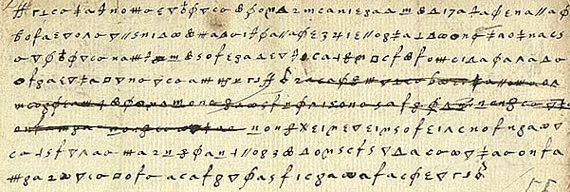
\includegraphics[width=\linewidth, height=1.5in, keepaspectratio]{../figure/encrypted_letter.jpg}
\caption{Snippet from encrypted communication between queen Mary and Sir
Babington}
\label{maryscottletterfig}
\end{marginfigure}

Mary used what's known as a \emph{substitution cipher} where each letter
is transformed into a different obscure symbol (see
\cref{maryscottletterfig}). At a first look, such a letter might seem
rather inscrutable- a meaningless sequence of strange symbols. However,
after some thought, one might recognize that these symbols \emph{repeat}
several times and moreover that different symbols repeat with different
frequencies. Now it doesn't take a large leap of faith to assume that
perhaps each symbol corresponds to a different letter and the more
frequent symbols correspond to letters that occur in the alphabet with
higher frequency. From this observation, there is a short gap to
completely breaking the cipher, which was in fact done by queen
Elisabeth's spies who used the decoded letters to learn of all the
co-conspirators and to convict queen Mary of treason, a crime for which
she was executed. Trusting in superficial security measures (such as
using ``inscrutable'' symbols) is a trap that users of cryptography have
been falling into again and again over the years. (As in many things,
this is the subject of a great XKCD cartoon, see \cref{XKCDnavajofig}.)

\begin{marginfigure}
\centering
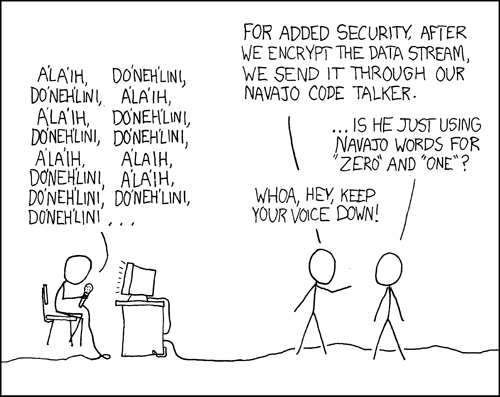
\includegraphics[width=\linewidth, height=1.5in, keepaspectratio]{../figure/code_talkers.png}
\caption{XKCD's take on the added security of using uncommon symbols}
\label{XKCDnavajofig}
\end{marginfigure}

The \href{https://en.wikipedia.org/wiki/Vigen\%C3\%A8re_cipher}{Vigenère
cipher} is named after Blaise de Vigenère who described it in a book in
1586 (though it was invented earlier by Bellaso). The idea is to use a
collection of substitution ciphers - if there are \(n\) different
ciphers then the first letter of the plaintext is encoded with the first
cipher, the second with the second cipher, the \(n^{th}\) with the
\(n^{th}\) cipher, and then the \(n+1^{st}\) letter is again encoded
with the first cipher. The key is usually a word or a phrase of \(n\)
letters, and the \(i^{th}\) substitution cipher is obtained by shifting
each letter \(k_i\) positions in the alphabet. This ``flattens'' the
frequencies and makes it much harder to do frequency analysis, which is
why this cipher was considered ``unbreakable'' for 300+ years and got
the nickname ``le chiffre indéchiffrable'' (``the unbreakable cipher'').
Nevertheless, Charles Babbage cracked the Vigenère cipher in 1854
(though he did not publish it). In 1863 Friedrich Kasiski broke the
cipher and published the result. The idea is that once you guess the
length of the cipher, you can reduce the task to breaking a simple
substitution cipher which can be done via frequency analysis (can you
see why?). Confederate generals used Vigenère regularly during the civil
war, and their messages were routinely cryptanalyzed by Union officers.

\begin{marginfigure}
\centering
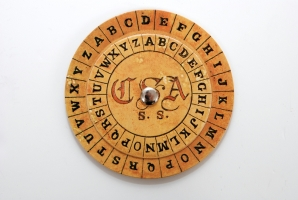
\includegraphics[width=\linewidth, height=1.5in, keepaspectratio]{../figure/confederate_cipher_disk.jpg}
\caption{Confederate Cipher Disk for implementing the Vigenère cipher}
\label{tmplabelfig}
\end{marginfigure}

\begin{marginfigure}
\centering
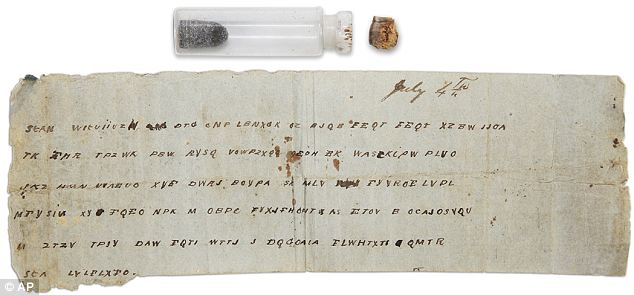
\includegraphics[width=\linewidth, height=1.5in, keepaspectratio]{../figure/confederate_message.jpg}
\caption{Confederate encryption of the message ``Gen'l Pemberton: You
can expect no help from this side of the river. Let Gen'l Johnston know,
if possible, when you can attack the same point on the enemy's lines.
Inform me also and I will endeavor to make a diversion. I have sent some
caps. I subjoin a despatch from General Johnston.''}
\label{tmplabelfig}
\end{marginfigure}

The \emph{Enigma} cipher was a mechanical cipher (looking like a
typewriter, see \cref{enigmafig}) where each letter typed would get
mapped into a different letter depending on the (rather complicated) key
and current state of the machine which had several rotors that rotated
at different paces. An identically wired machine at the other end could
be used to decrypt. Just as many ciphers in history, this has also been
believed by the Germans to be ``impossible to break'' and even quite
late in the war they refused to believe it was broken despite mounting
evidence to that effect. (In fact, some German generals refused to
believe it was broken even \emph{after} the war.) Breaking Enigma was an
heroic effort which was initiated by the Poles and then completed by the
British at Bletchley Park, with Alan Turing (of the Turing machines)
playing a key role. As part of this effort the Brits built arguably the
world's first large scale mechanical computation devices (though they
looked more similar to washing machines than to iPhones). They were also
helped along the way by some quirks and errors of the German operators.
For example, the fact that their messages ended with ``Heil Hitler''
turned out to be quite useful.

\begin{marginfigure}
\centering
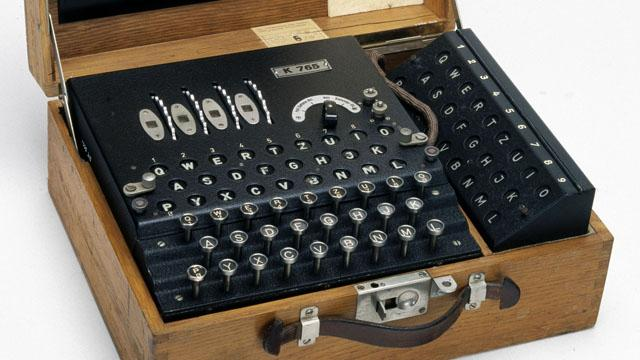
\includegraphics[width=\linewidth, height=1.5in, keepaspectratio]{../figure/enigma.jpg}
\caption{In the \emph{Enigma} mechanical cipher the secret key would be
the settings of the rotors and internal wires. As the operator types up
their message, the encrypted version appeared in the display area above,
and the internal state of the cipher was updated (and so typing the same
letter twice would generally result in two different letters output).
Decrypting follows the same process: if the sender and receiver are
using the same key then typing the ciphertext would result in the
plaintext appearing in the display.}
\label{enigmafig}
\end{marginfigure}

Here is one entertaining anecdote: the Enigma machine would never map a
letter to itself. In March 1941, Mavis Batey, a cryptanalyst at
Bletchley Park received a very long message that she tried to decrypt.
She then noticed a curious property--- the message did \emph{not}
contain the letter ``L''.\footnote{Here is a nice exercise: compute (up
  to an order of magnitude) the probability that a 50-letter long
  message composed of random letters will end up not containing the
  letter ``L''.} She realized that the probability that no ``L'''s
appeared in the message is too small for this to happen by chance. Hence
she surmised that the original message must have been composed
\emph{only} of L's. That is, it must have been the case that the
operator, perhaps to test the machine, have simply sent out a message
where he repeatedly pressed the letter ``L''. This observation helped
her decode the next message, which helped inform of a planned Italian
attack and secure a resounding British victory in what became known as
``the Battle of Cape Matapan''. Mavis also helped break another Enigma
machine. Using the information she provided, the Brits were able to feed
the Germans with the false information that the main allied invasion
would take place in Pas de Calais rather than on Normandy.

In the words of General Eisenhower, the intelligence from Bletchley park
was of ``priceless value''. It made a huge difference for the Allied war
effort, thereby shortening World War II and saving millions of lives.
See also \href{http://www.cix.co.uk/~klockstone/hinsley.htm}{this
interview with Sir Harry Hinsley}.

\section{Defining encryptions}\label{1-Defining-encryptions}

Many of the troubles that cryptosystem designers faced over history (and
still face!) can be attributed to not properly defining or understanding
what the goals they want to achieve are in the first place. We now turn
to actually defining what is an encryption scheme. Clearly we can encode
every message as a string of bits, i.e., an element of \(\{0,1\}^\ell\)
for some \(\ell\). Similarly, we can encode the \emph{key} as a string
of bits as well, i.e., an element of \(\{0,1\}^n\) for some \(n\). Thus,
we can think of an encryption scheme as composed of two functions. The
\emph{encryption function} \(E\) maps a secret key \(k \in \{0,1\}^n\)
and a message (known also as \emph{plaintext}) \(m\in \{0,1\}^\ell\)
into a \emph{ciphertext} \(c \in \{0,1\}^L\) for some \(L\). We write
this as \(c = E_k(m)\). The \emph{decryption function} \(D\) does the
reverse operation, mapping the secret key \(k\) and the ciphertext \(c\)
back into the plaintext message \(m\), which we write as \(m = D_k(c)\).
The basic equation is that if we use the same key for encryption and
decryption, then we should get the same message back. That is, for every
\(k \in \{0,1\}^n\) and \(m\in \{0,1\}^\ell\),

\begin{equation*}
m = D_k(E_k(m)) \;.
\end{equation*}

This motivates the following definition which attempts to capture what
it means for an encryption scheme to be \emph{valid} or ``make sense'',
regardless of whether or not it is \emph{secure}:

\hypertarget{encryptiondef}{}
\begin{definition}[Valid encryption scheme] \label[definition]{encryptiondef}

Let \(\ell:\N \rightarrow \N\) and \(C:\N \rightarrow \N\) be two
functions mapping natural numbers to natural numbers. A pair of
polynomial-time computable functions \((E,D)\) mapping strings to
strings is a \emph{valid private key encryption scheme} (or
\emph{encryption scheme} for short) with plaintext length function
\(\ell(\cdot)\) and ciphertext length function \(C(\cdot)\) if for every
\(n\in \N\), \(k\in \{0,1\}^n\) and \(m \in \{0,1\}^{\ell(n)}\),
\(|E_k(m)|= C(n)\) and \[
D(k,E(k,m))=m \;. \label{eqvalidenc}
\]

\end{definition}

We will often write the first input (i.e., the key) to the encryption
and decryption as a subscript and so can write \eqref{eqvalidenc} also
as \(D_k(E_k(m))=m\).

\begin{figure}
\centering
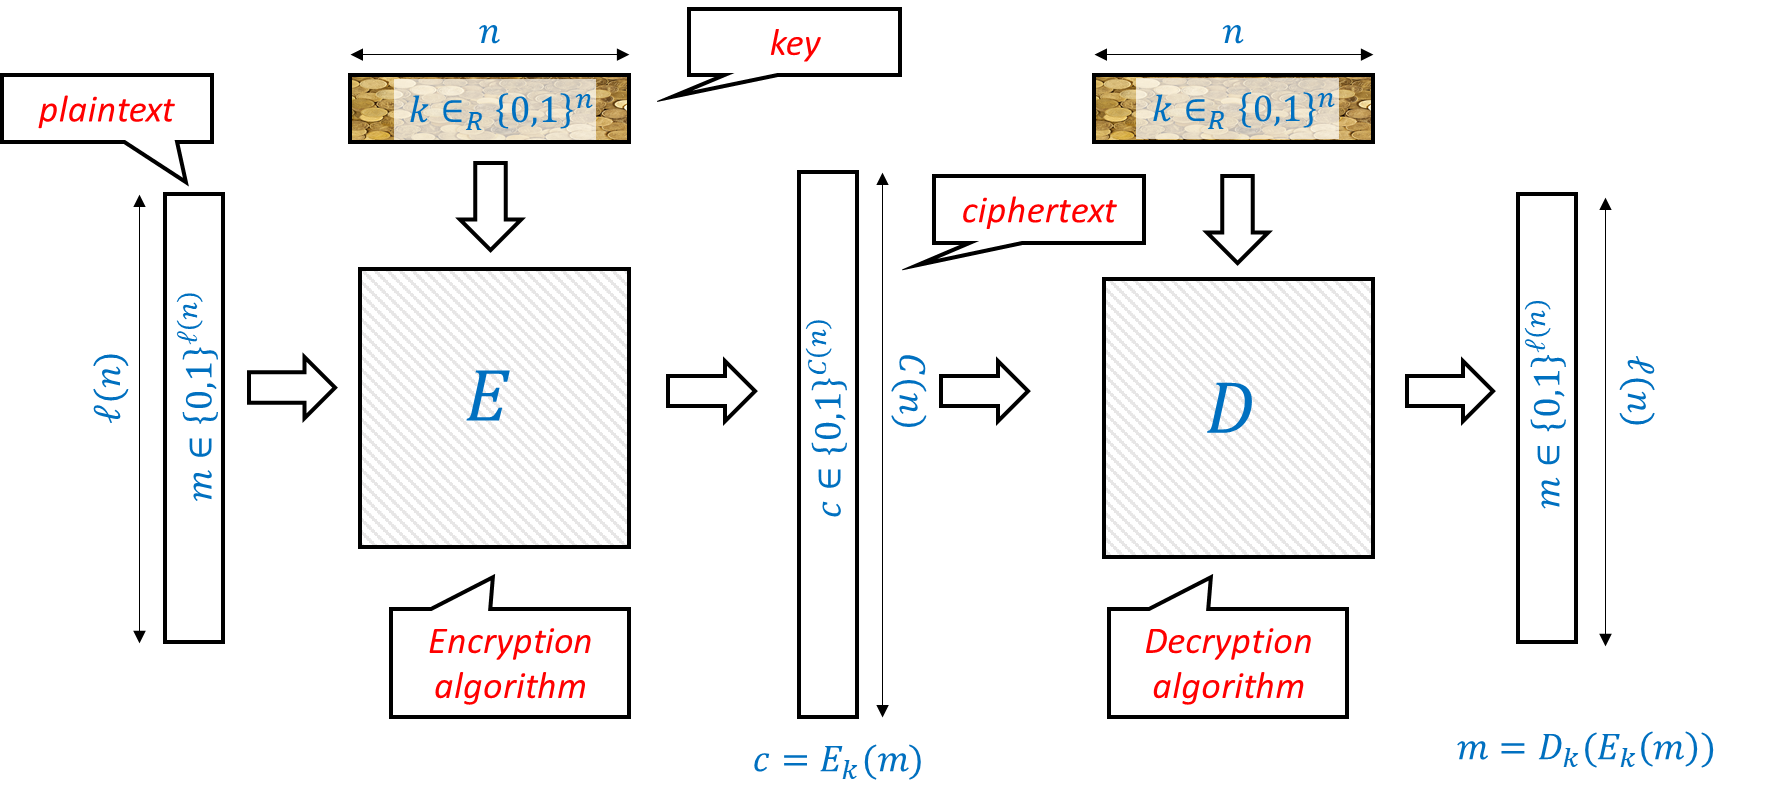
\includegraphics[width=\textwidth, height=0.25\paperheight, keepaspectratio]{../figure/valid_encryption_fig.png}
\caption{A private-key encryption scheme is a pair of algorithms \(E,D\)
such that for every key \(k\in \{0,1\}^n\) and plaintext
\(x\in \{0,1\}^{\ell(n)}\), \(c=E_k(m)\) is a ciphertext of length
\(C(n)\). The encryption scheme is \emph{valid} if for every such \(y\),
\(D_k(y)=x\). That is, the decryption of an encryption of \(x\) is
\(x\), as long as both encryption and decryption use the same key.}
\label{validencryption}
\end{figure}

The validity condition implies that for any fixed \(k\), the map
\(m \mapsto E_k(m)\) is one to one (can you see why?) and hence the
ciphertext length is always at least the plaintext length. Thus we
typically focus on the plaintext length as the quantity to optimize in
an encryption scheme. The \emph{larger} \(\ell(n)\) is, the better the
scheme, since it means we need a shorter secret key to protect messages
of the same length.

\hypertarget{notation}{}
\begin{remark}[A note on notation, and comparison with Katz-Lindell, Boneh-Shoup, and other texts.] \label[remark]{notation}

\emph{A note on notation:} We will always use \(i,j,\ell,n\) to denote
natural numbers.

The number \(n\) will often denote the length of our secret key. The
length of the key (or another closely related number) is often known as
the \emph{security parameter} in the literature. Katz-Lindell also uses
\(n\) to denote this parameter, while Boneh-Shoup and Rosulek use
\(\lambda\) for it. (Some texts also use the Greek letter \(\kappa\) for
the same parameter.) We chose to denote the security parameter by \(n\)
as to correspond with the standard algorithmic notation for input length
(as in \(O(n)\) or \(O(n^2)\) time algorithms).

We often use \(\ell\) to denote the length of the message, sometimes
also known as ``block length'' since longer messages are simply chopped
into ``blocks'' of length \(\ell\) and also appropriately padded.

We will use \(k\) to denote the secret key, \(m\) to denote the secret
plaintext message, and \(c\) to denote the encrypted ciphertext. Note
that \(k,m,c\) are not numbers but rather bit strings of lengths
\(n,\ell(n),C(n)\) respectively. We will also sometimes use \(x\) and
\(y\) to denote strings, and so sometimes use \(x\) as the plaintext and
\(y\) as the ciphertext. In general, while we try to reserve variable
names for particular purposes, cryptography uses so many concepts that
it would sometimes need to ``reuse'' the same letter for different
purposes.

For simplicity, we denote the space of possible keys as \(\{0,1\}^n\)
and the space of possible messages as \(\{0,1\}^\ell\) for
\(\ell=\ell(n)\). Boneh-Shoup uses a more general notation of
\(\mathcal{K}\) for the space of all possible keys and \(\mathcal{M}\)
for the space of all possible messages. This does not make much
difference since we can represent every discrete object such as a key or
message as a binary string. (One difference is that in principle the
space of all possible messages could include messages of unbounded
length, though in such a case what is done in both theory and practice
is to break these up into finite-size blocks and encrypt one block at a
time.)

\end{remark}

\section{Defining security of
encryption}\label{1-Defining-security-of-e}

\cref{encryptiondef} says nothing about security and does not rule out
trivial ``encryption'' schemes such as the scheme \(E_k(m) = m\) that
simply outputs the plaintext as is. Defining security is tricky, and
we'll take it one step at a time, but let's start by pondering what is
secret and what is not. A priori we are thinking of an attacker Eve that
simply sees the ciphertext \(c=E_k(m)\) and does not know anything on
how it was generated. So, it does not know the details of \(E\) and
\(D\), and certainly does not know the secret key \(k\). However, many
of the troubles past cryptosystems went through were caused by them
relying on ``security through obscurity''--- trusting that the fact
their \emph{methods} are not known to their enemy will protect them from
being broken. This is a faulty assumption - if you reuse a method again
and again (even with a different key each time) then eventually your
adversaries will figure out what you are doing. And if Alice and Bob
meet frequently in a secure location to decide on a new method, they
might as well take the opportunity to exchange their secret
messages\ldots{}

These considerations led Auguste Kerckhoffs in 1883 to state the
following principle:

\begin{quote}
\emph{A cryptosystem should be secure even if everything about the
system, except the key, is public knowledge.}\footnote{The actual quote
  is ``Il faut qu'il n'exige pas le secret, et qu'il puisse sans
  inconvénient tomber entre les mains de l'ennemi'' loosely translated
  as ``The system must not require secrecy and can be stolen by the
  enemy without causing trouble''. According to Steve Bellovin the NSA
  version is ``assume that the first copy of any device we make is
  shipped to the Kremlin''.}
\end{quote}

Why is it OK to assume the key is secret and not the algorithm? Because
we can always choose a fresh key. But of course that won't help us much
if our key is ``1234'' or ``passw0rd!''. In fact, if you use \emph{any}
deterministic algorithm to choose the key then eventually your adversary
will figure this out. Therefore for security we must choose the key at
\emph{random} and can restate Kerckhoffs's principle as follows:

\begin{quote}
\emph{There is no secrecy without randomness}
\end{quote}

This is such a crucial point that is worth repeating:

\begin{quote}
\emph{There is no secrecy without randomness}
\end{quote}

At the heart of every cryptographic scheme there is a secret key, and
the secret key is always chosen at random. A corollary of that is that
to understand cryptography, you need to know some probability theory.
Fortunately, we don't need much of probability- only probability over
finite spaces, and basic notions such as expectation, variance,
concentration and the union bound suffice for most of we need. In fact,
understanding the following two statements will already get you much of
what you need for cryptography:

\begin{itemize}
\item
  For every fixed string \(x\in\{0,1\}^n\), if you toss a coin \(n\)
  times, the probability that the heads/tails pattern will be exactly
  \(x\) is \(2^{-n}\).
\item
  A probability of \(2^{-128}\) is really really small.
\end{itemize}

\subsection{Generating randomness in actual cryptographic
systems}\label{1-Generating-randomness-}

How do we actually get random bits in actual systems? The main idea is
to use a two stage approach. First we need to get some data that is
\emph{unpredictable} from the point of view of an attacker on our
system. Some sources for this could be measuring latency on the network
or hard drives (getting harder with solid state disk), user keyboard and
mouse movement patterns (problematic when you need fresh randomness at
boot time ), clock drift and more, there are some other sources
including audio, video, and network. All of these can be problematic,
especially for servers or virtual machines, and so hardware based random
number generators based on phenomena such as thermal noise or nuclear
decay are becoming more popular. Once we have some data \(X\) that is
unpredictable, we need to estimate the \emph{entropy} in it. You can
roughly imagine that \(X\) has \(k\) bits of entropy if the probability
that an attacker can guess \(X\) is at most \(2^{-k}\). People then use
a \emph{hash function} (an object we'll talk about more later) to map
\(X\) into a string of length \(k\) which is then hopefully distributed
(close to) uniformly at random. All of this process, and especially
understanding the amount of information an attacker may have on the
entropy sources, is a bit of a dark art and indeed a number of attacks
on cryptographic systems were actually enabled by weak generation of
randomness. Here are a few examples.

One of the first attacks was on the SSL implementation of Netscape
(\emph{the} browser at the time). Netscape used the following
``unpredictable'' information--- the time of day and a process ID both
of which turned out to be quite predictable (who knew attackers have
clocks too?). Netscape tried to protect its security through ``security
through obscurity'' by not releasing the source code for their
pseudorandom generator, but it was reverse engineered by
\href{https://www.cs.berkeley.edu/~daw/papers/ddj-netscape.html}{Ian
Goldberg and David Wagner} (Ph.D students at the time) who demonstrated
this attack.

In 2006 a programmer removed a line of code from the procedure to
generate entropy in OpenSSL package distributed by Debian since it
caused a warning in some automatic verification code. As a result for
two years (until this was discovered) all the randomness generated by
this procedure used only the process ID as an ``unpredictable'' source.
This means that all communication done by users in that period is fairly
easily breakable (and in particular, if some entities recorded that
communication they could break it also retroactively). This caused a
huge headache and a worldwide regeneration of keys, though it is
believed that many of the weak keys are still used. See
\href{http://www.xkcd.com/424/}{XKCD's take} on that incident.

\begin{marginfigure}
\centering
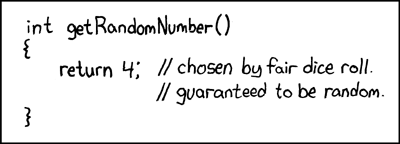
\includegraphics[width=\linewidth, height=1.5in, keepaspectratio]{../figure/random_number.png}
\caption{XKCD Cartoon: Random number generator}
\label{tmplabelfig}
\end{marginfigure}

In 2012 two separate teams of researchers scanned a large number of RSA
keys on the web and found out that about 4 percent of them are easy to
break. The main issue were devices such as routers, internet-connected
printers and such. These devices sometimes run variants of Linux- a
desktop operating system- but without a hard drive, mouse or keyboard,
they don't have access to many of the entropy sources that desktops
have. Coupled with some good old fashioned ignorance of cryptography and
software bugs, this led to many keys that are downright trivial to
break, see
\href{https://freedom-to-tinker.com/blog/nadiah/new-research-theres-no-need-panic-over-factorable-keys-just-mind-your-ps-and-qs/}{this
blog post} and \href{https://factorable.net/}{this web page} for more
details.

After the entropy is collected and then ``purified'' or ``extracted'' to
a uniformly random string that is, say, a few hundred bits long, we
often need to ``expand'' it into a longer string that is also uniform
(or at least looks like that for all practical purposes). We will
discuss how to go about that in the next lecture. This step has its
weaknesses too, and in particular the Snowden documents, combined with
observations of Shumow and Ferguson, strongly suggest that the NSA has
deliberately inserted a \emph{trapdoor} in one of the pseudorandom
generators published by the National Institute of Standards and
Technologies (NIST). Fortunately, this generator wasn't widely adopted,
but apparently the NSA did pay 10 million dollars to RSA security so the
latter would make this generator their default option in their products.

\section{Defining the secrecy
requirement.}\label{1-Defining-the-secrecy-r}

Defining the secrecy requirement for an encryption is not simple. Over
the course of history, many smart people got it wrong and convinced
themselves that ciphers were impossible to break. The first person to
truly ask the question in a rigorous way was Claude Shannon in 1945
(though a partial version of his manuscript was only declassified in
1949). Simply by asking this question, he made an enormous contribution
to the science of cryptography and practical security. We now will try
to examine how one might answer it.

Let me warn you ahead of time that we are going to insist on a
\emph{mathematically precise definition} of security. That means that
the definition must capture security in all cases, and the existence of
a single counterexample, no matter how ``silly'', would make us rule out
a candidate definition. This exercise of coming up with ``silly''
counterexamples might seem, well, silly. But in fact it is this method
that has led Shannon to formulate his theory of secrecy, which (after
much followup work) eventually revolutionized cryptography, and brought
this science to a new age where Edgar Allan Poe's maxim no longer holds,
and we are able to design ciphers which human (or even nonhuman)
ingenuity cannot break.

The most natural way to attack an encryption is for Eve to guess all
possible keys. In many encryption schemes this number is enormous and
this attack is completely infeasible. For example, the theoretical
number of possibilities in the Enigma cipher was about \(10^{113}\)
which roughly means that even if we filled the milky way galaxy with
computers operating at light speed, the sun would still die out before
it finished examining all the possibilities.\footnote{There are about
  \(10^{68}\) atoms in the galaxy, so even if we assumed that each one
  of those atoms was a computer that can process say \(10^{21}\)
  decryption attempts per second (as the speed of light is \(10^9\)
  meters per second and the diameter of an atom is about \(10^{-12}\)
  meters), then it would still take \(10^{113-89} = 10^{24}\) seconds,
  which is about \(10^{17}\) years to exhaust all possibilities, while
  the sun is estimated to burn out in about 5 billion years.} One can
understand why the Germans thought it was impossible to break. (Note
that despite the number of possibilities being so enormous, such a key
can still be easily specified and shared between Alice and Bob by
writing down \(113\) digits on a piece of paper.) Ray Miller of the NSA
had calculated that, in the way the Germans used the machine, the number
of possibilities was ``only'' \(10^{23}\), but this is still extremely
difficult to pull off even today, and many orders of magnitudes above
the computational powers during the WW-II era. Thus clearly, it is
sometimes possible to break an encryption without trying all
possibilities. A corollary is that having a huge number of key
combinations does not guarantee security, as an attacker might find a
shortcut (as the allies did for Enigma) and recover the key without
trying all options.

Since it is possible to recover the key with some tiny probability
(e.g.~by guessing it at random), perhaps one way to define security of
an encryption scheme is that an attacker can never recover the key with
probability significantly higher than that. Here is an attempt at such a
definition:

\hypertarget{securefirstattemptdef}{}
\begin{definition}[Security of encryption: first attempt] \label[definition]{securefirstattemptdef}

An encryption scheme \((E,D)\) is \emph{\(n\)-secure} if no matter what
method Eve employs, the probability that she can recover the true key
\(k\) from the ciphertext \(c\) is at most \(2^{-n}\).

\end{definition}

\begin{pause} \label[pause]{1-When-you-see-a-mathema}

When you see a mathematical definition that attempts to model some
real-life phenomenon such as security, you should pause and ask
yourself:

\begin{enumerate}
\def\labelenumi{\arabic{enumi}.}
\item
  Do I understand mathematically what the definition is stating?\\
\item
  Is it a reasonable way to capture the real life phenomenon we are
  discussing?
\end{enumerate}

One way to answer question 2 is to try to think of both examples of
objects that satisfy the definition and examples of objects that violate
it, and see if this conforms to your intuition about whether these
objects display the phenomenon we are trying to capture. Try to do this
for \cref{securefirstattemptdef}

\end{pause}

You might wonder if \cref{securefirstattemptdef} is not \emph{too
strong}. After all how are we going to ever prove that Eve cannot
recover the secret key no matter what she does? Edgar Allan Poe would
say that there can always be a method that we overlooked. However, in
fact this definition is too \emph{weak}! Consider the following
encryption: the secret key \(k\) is chosen at random in \(\{0,1\}^n\)
but our encryption scheme simply ignores it and lets \(E_k(m)=m\) and
\(D_k(c)=c\). This is a valid encryption since \(D_k(E_k(m))=m\), but is
of course completely insecure as we are simply outputting the plaintext
in the clear. Yet, no matter what Eve does, if she only sees \(c\) and
not \(k\), there is no way she can guess the true value of \(k\) with
probability better than \(2^{-n}\), since it was chosen completely at
random and she gets no information about it. Formally, one can prove the
following result:

\hypertarget{trivialsec}{}
\begin{lemma} \label[lemma]{trivialsec}

Let \((E,D)\) be the encryption scheme above. For every function
\(Eve:\{0,1\}^\ell\rightarrow \{0,1\}^n\) and for every
\(m\in \{0,1\}^\ell\), the probability that \(Eve(E_k(m))=k\) is exactly
\(2^{-n}\).

\end{lemma}

\begin{proof} \label[proof]{1-This-follows-because-E}

This follows because \(E_k(m)=m\) and hence \(Eve(E_k(m))=Eve(m)\) which
is some fixed value \(k'\in\{0,1\}^n\) that is independent of \(k\).
Hence the probability that \(k=k'\) is \(2^{-n}\). QED

\end{proof}

The math behind the above argument is very simple, yet I urge you to
read and re-read the last two paragraphs until you are sure that you
completely understand why this encryption is in fact secure according to
the above definition. This is a ``toy example'' of the kind of reasoning
that we will be employing constantly throughout this course, and you
want to make sure that you follow it.

So, \cref{trivialsec} is true, but one might question its meaning.
Clearly this silly example was not what we meant when stating this
definition. However, as mentioned above, we are not willing to ignore
even silly examples and must amend the definition to rule them out. One
obvious objection is that we don't care about hiding the key- it is the
\emph{message} that we are trying to keep secret. This suggests the next
attempt:

\hypertarget{securesecondattemptdef}{}
\begin{definition}[Security of encryption: second attempt] \label[definition]{securesecondattemptdef}

An encryption scheme \((E,D)\) is \emph{\(n\)-secure} if for every
message \(m\) no matter what method Eve employs, the probability that
she can recover \(m\) from the ciphertext \(c=E_k(m)\) is at most
\(2^{-n}\).

\end{definition}

Now this seems like it captures our intended meaning. But remember that
we are being anal, and truly insist that the definition holds as stated,
namely that for every plaintext message \(m\) and every function
\(Eve:\{0,1\}^C\rightarrow\{0,1\}^\ell\), the probability over the
choice of \(k\) that \(Eve(E_k(m))=m\) is at most \(2^{-n}\). But now we
see that this is clearly impossible. After all, this is supposed to work
for \emph{every} message \(m\) and \emph{every} function \(Eve\), but
clearly if \(m\) is the all-zeroes message \(0^\ell\) and \(Eve\) is the
function that ignores its input and simply outputs \(0^\ell\), then it
will hold that \(Eve(E_k(m))=m\) with probability one.

So, if before the definition was too weak, the new definition is too
strong and is impossible to achieve. The problem is that of course we
could guess a fixed message with probability one, so perhaps we could
try to consider a definition with a \emph{random} message. That is:

\hypertarget{securethirdattemptdef}{}
\begin{definition}[Security of encryption: third attempt] \label[definition]{securethirdattemptdef}

An encryption scheme \((E,D)\) is \emph{\(n\)-secure} if no matter what
method Eve employs, if \(m\) is chosen at random from \(\{0,1\}^\ell\),
the probability that she can recover \(m\) from the ciphertext
\(c=E_k(m)\) is at most \(2^{-n}\).

\end{definition}

This weakened definition can in fact be achieved, but we have again
weakened it too much. Consider an encryption that hides the last
\(\ell/2\) bits of the message, but completely reveals the first
\(\ell/2\) bits. The probability of guessing a random message is
\(2^{-\ell/2}\), and so such a scheme would be ``\(\ell/2\) secure'' per
\cref{securethirdattemptdef} but this is still a scheme that you would
not want to use. The point is that in practice we don't encrypt random
messages--- our messages might be in English, might have common headers,
and might have even more structures based on the context. In fact, it
may be that the message is either ``Yes'' or ``No'' (or perhaps either
``Attack today'' or ``Attack tomorrow'') but we want to make sure Eve
doesn't learn which one it is. So, using an encryption scheme that
reveals the first half of the message (or frankly even only the first
bit) is unacceptable.

\section{Perfect Secrecy}\label{1-Perfect-Secrecy}

So far all of our attempts at definitions oscillated between being too
strong (and hence impossible) or too weak (and hence not guaranteeing
actual security). The key insight of Shannon was that in a secure
encryption scheme the ciphertext should not reveal \emph{any additional
information} about the plaintext. So, if for example it was a priori
possible for Eve to guess the plaintext with some probability \(1/k\)
(e.g., because there were only \(k\) possibilities for it) then she
should not be able to guess it with higher probability after seeing the
ciphertext. This can be formalized as follows:

\hypertarget{perfectsecrecydef}{}
\begin{definition}[Perfect secrecy] \label[definition]{perfectsecrecydef}

An encryption scheme \((E,D)\) is \emph{perfectly secret} if there for
every set \(M\subseteq\{0,1\}^\ell\) of plaintexts, and for every
strategy used by Eve, if we choose at random \(m\in M\) and a random key
\(k\in\{0,1\}^n\), then the probability that Eve guesses \(m\) after
seeing \(E_k(m)\) is at most \(1/|M|\).

\end{definition}

In particular, if we encrypt either ``Yes'' or ``No'' with probability
\(1/2\), then Eve won't be able to guess which one it is with
probability better than half. In fact, that turns out to be the heart of
the matter:

\hypertarget{twotomanythm}{}
\begin{theorem}[Two to many theorem] \label[theorem]{twotomanythm}

An encryption scheme \((E,D)\) is perfectly secret if and only if for
every two distinct plaintexts \(\{m_0,m_1\} \subseteq \{0,1\}^\ell\) and
every strategy used by Eve, if we choose at random \(b\in\{0,1\}\) and a
random key \(k\in\{0,1\}^n\), then the probability that Eve guesses
\(m_b\) after seeing \(E_k(m_b)\) is at most \(1/2\).

\end{theorem}

\begin{proof} \label[proof]{1-The-only-if-direction-}

The ``only if'' direction is obvious--- this condition is a special case
of the perfect secrecy condition for a set \(M\) of size \(2\).

The ``if'' direction is trickier. We will use a proof by contradiction.
We need to show that if there is some set \(M\) (of size possibly much
larger than \(2\)) and some strategy for Eve to guess (based on the
ciphertext) a plaintext chosen from \(M\) with probability larger than
\(1/|M|\), then there is also some set \(M'\) of size two and a strategy
\(Eve'\) for Eve to guess a plaintext chosen from \(M'\) with
probability larger than \(1/2\).

Let's fix the message \(m_0\) to be the all zeroes message and pick
\(m_1\) at random in \(M\). Under our assumption, it holds that for
random key \(k\) and message \(m_1\in M\),
\[\Pr_{k \leftarrow_R \{0,1\}^n, m_1 \leftarrow_R M}[Eve(E_k(m_1))=m_1] > 1/|M|\;. \label{eqabovetrivialcipher}\]
On the other hand, for every choice of \(k\), \(m'= Eve(E_k(m_0))\) is a
fixed string independent on the choice of \(m_1\), and so if we pick
\(m_1\) at random in \(M\), then the probability that \(m_1=m'\) is at
most \(1/|M|\), or in other words

\[\Pr_{k \leftarrow_R \{0,1\}^n, m_1 \leftarrow_R M}[Eve(E_k(m_0))=m_1] \leq 1/|M|\;. \label{eqhitcipher}\]

We can also write \eqref{eqabovetrivialcipher} and \eqref{eqhitcipher}
as
\begin{equation*}
\E_{m_1 \leftarrow_R M} \Pr[ Eve(E_k(m_1))=m_1] > 1/|M|
\end{equation*}
and
\begin{equation*}
\E_{m_1 \leftarrow_R M} \Pr[ Eve(E_k(m_0))=m_1] \leq 1/|M|
\end{equation*}
where these expectations are taken over the choice of \(m_1\). Hence by
linearity of expectation \[
\E_{m_1 \leftarrow_R M} \left( \Pr[ Eve(E_k(m_1))=m_1] - \Pr[ Eve(E_k(m_0))=m_1] \right) > 0 \;. \label{eqadvantageciphermonevsmzero}
\] (In words, for random \(m_1\), the probability that Eve outputs
\(m_1\) given an encryption of \(m_1\) is higher than the probability
that Eve outputs \(m_1\) given an encryption of \(m_0\).)

In particular, by the \emph{averaging argument} (the argument that if
the average of numbers is larger than \(\alpha\) then one of the numbers
is larger than \(\alpha\)) there must \emph{exist} \(m_1 \in M\)
satisfying
\begin{equation*}
\Pr[Eve(E_k(m_1))=m_1] > \Pr[Eve(E_k(m_0))=m_1] \;.
\end{equation*}
(Can you see why? This is worthwhile stopping and reading again.)

But this can be turned into an attacker \(Eve'\) such that for
\(b \leftarrow_R \{0,1\}\). the probability that \(Eve'(E_k(m_b))=m_b\)
is larger than \(1/2\). Indeed, we can define \(Eve'(c)\) to output
\(m_1\) if \(Eve(c)=m_1\) and otherwise output a random message in
\(\{ m_0 , m_1 \}\). The probability that \(Eve'(y)\) equals \(m_1\) is
higher when \(c=E_k(m_1)\) than when \(c=E_k(m_0)\), and since \(Eve'\)
outputs either \(m_0\) or \(m_1\), this means that the probability that
\(Eve'(E_k(m_b))=m_b\) is larger than \(1/2\). (Can you see why?)

\end{proof}

\begin{pause} \label[pause]{1-The-proof-of-creftwoto}

The proof of \cref{twotomanythm} is not trivial, and is worth reading
again and making sure you understand it. An excellent exercise, which I
urge you to pause and do now is to prove the following: \((E,D)\) is
perfectly secret if for every plaintexts \(m,m' \in \{0,1\}^\ell\), the
two random variables \(\{ E_k(m) \}\) and \(\{ E_{k'}(m') \}\) (for
randomly chosen keys \(k\) and \(k'\)) have precisely the same
distribution.

\end{pause}

\hypertarget{perfectsecrecyequiv}{}
\begin{solvedexercise}[Perfect secrecy, equivalent definition] \label[solvedexercise]{perfectsecrecyequiv}

Prove that a valid encryption scheme \((E,D)\) with plaintext length
\(\ell(\cdot)\) is perfectly secret if and only if for every \(n\in \N\)
and plaintexts \(m,m' \in \{0,1\}^{\ell(n)}\), the following two
distributions \(Y\) and \(Y'\) over \(\{0,1\}^*\) are identical:

\begin{itemize}
\item
  \(Y\) is obtained by sampling \(k\leftarrow_R \{0,1\}^n\) and
  outputting \(E_k(m)\).
\item
  \(Y'\) is obtained by sampling \(k\leftarrow_R \{0,1\}^n\) and
  outputting \(E_k(m')\).
\end{itemize}

\end{solvedexercise}

\begin{solution} \label[solution]{1-We-only-sketch-the-pro}

We only sketch the proof. The condition in the exercise is equivalent to
perfect secrecy with \(|M|=2\). For every \(M = \{ m,m' \}\), if \(Y\)
and \(Y'\) are identical then clearly for every \(Eve\) and possible
output \(y\), \(\Pr[ Eve(E_k(m))=y] = \Pr[ Eve(E_k(m'))=y]\) since these
correspond applying \(Eve\) on the same distribution \(Y=Y'\). On the
other hand, if \(Y\) and \(Y'\) are not identical then there must exist
some ciphertext \(c^*\) such that \(\Pr[ Y=c^*] > \Pr[ Y'=c^*]\) (or
vice versa). The adversary that on input \(c\) guesses that \(c\) is an
encryption of \(m\) if \(c=c^*\) and otherwise tosses a coin will have
some advantage over \(1/2\) in distinguishing an encryption of \(m\)
from an encryption of \(m'\).

\end{solution}

We summarize the equivalent definitions of perfect secrecy in the
following theorem, whose (omitted) proof follows from
\cref{twotomanythm} and \cref{perfectsecrecyequiv} as well as similar
proof ideas.

\hypertarget{perfectsecrecythm}{}
\begin{theorem}[Perfect secrecy equivalent conditions] \label[theorem]{perfectsecrecythm}

Let \((E,D)\) be a valid encryption scheme with message length
\(\ell(n)\). Then the following conditions are equivalent:

\begin{enumerate}
\def\labelenumi{\arabic{enumi}.}
\item
  \((E,D)\) is perfectly secret as per \cref{perfectsecrecydef}.
\item
  For every pair of messages \(m_0,m_1 \in \{0,1\}^{\ell(n)}\), the
  distributions \(\{ E_k(m_0) \}_{k \leftarrow_R \{0,1\}^n}\) and
  \(\{ E_k(m_1) \}_{k \leftarrow_R \{0,1\}^n}\) are identical.
\item
  (Two-message security: Eve can't guess which of one of two messages
  was encrypted with success better than half.) For every function
  \(Eve:\{0,1\}^{C(n)} \rightarrow \{0,1\}^{\ell(n)}\) and pair of
  messages \(m_0,m_1 \in \{0,1\}^{\ell(n)}\),
\end{enumerate}

\begin{equation*}
\Pr_{b \leftarrow_R \{0,1\}, k \leftarrow_R \{0,1\}^n} [ Eve(E_k(m_b))=m_b ] \leq 1/2
\end{equation*}

\begin{enumerate}
\def\labelenumi{\arabic{enumi}.}
\setcounter{enumi}{3}
\tightlist
\item
  (Arbitrary prior security: Eve can't guess which message was encrypted
  with success better than her prior information.) For every
  distribution \(\mathcal{D}\) over \(\{0,1\}^{\ell(n)}\), and
  \(Eve:\{0,1\}^{C(n)} \rightarrow \{0,1\}^{\ell(n)}\),
\end{enumerate}

\begin{equation*}
\Pr_{m \leftarrow_R \mathcal{D}, k \leftarrow_R \{0,1\}^n}[ Eve(E_k(m))=m ] \leq \max(\mathcal{D})
\end{equation*}

where we denote
\(\max(\mathcal{D}) = \max_{m^*\in \{0,1\}^{\ell(n)}} \Pr_{m \leftarrow_R \mathcal{D}}[m=m^*]\)
to be the largest probability of any element under \(\mathcal{D}\).

\end{theorem}

\subsection{Achieving perfect secrecy}\label{1-Achieving-perfect-secr}

So, perfect secrecy is a natural condition, and does not seem to be too
weak for applications, but can it actually be achieved? After all, the
condition that two different plaintexts are mapped to the same
distribution seems somewhat at odds with the condition that Bob would
succeed in decrypting the ciphertexts and find out if the plaintext was
in fact \(m\) or \(m'\). It turns out the answer is yes! For example,
\cref{onetimepadtwofig} details a perfectly secret encryption for two
bits.

\begin{figure}
\centering
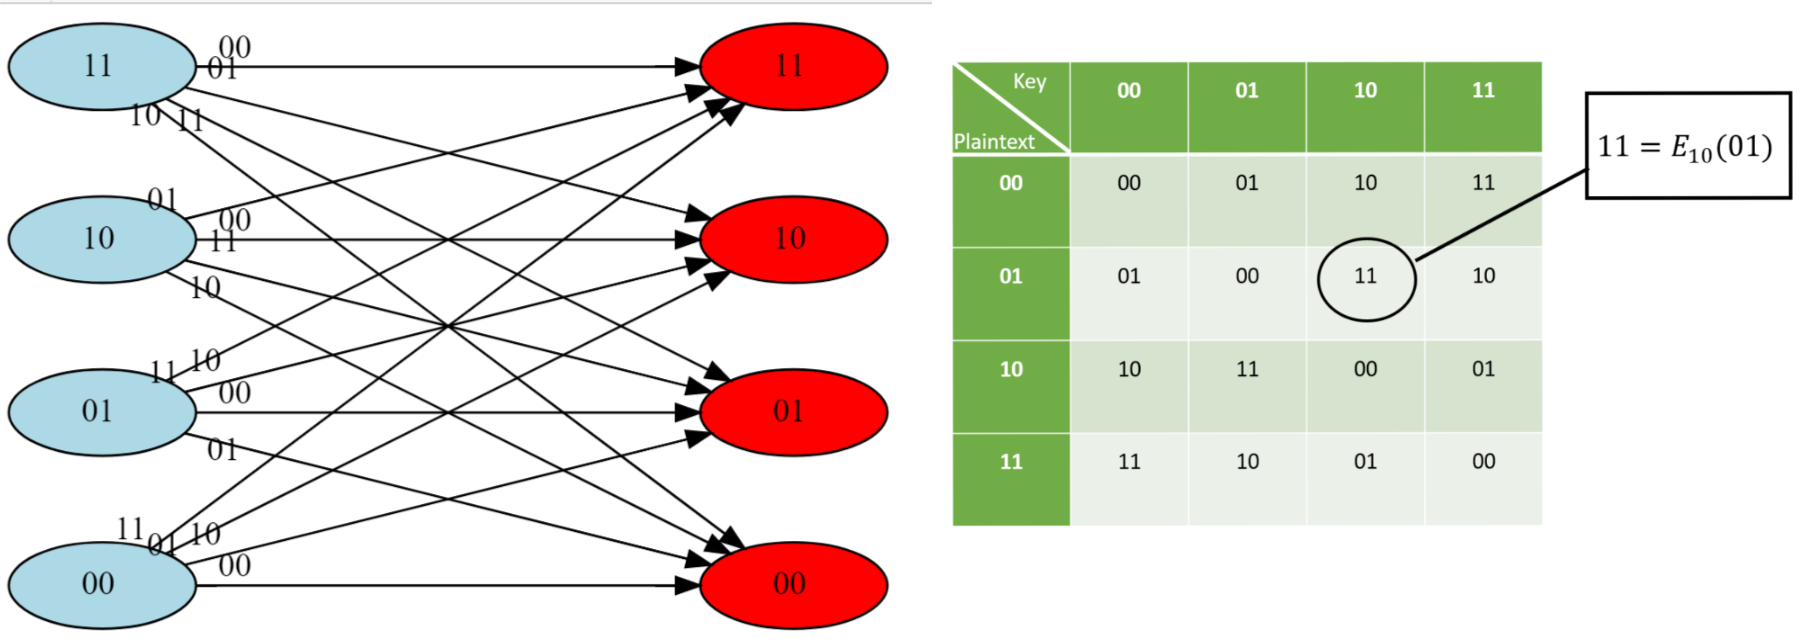
\includegraphics[width=\textwidth, height=0.25\paperheight, keepaspectratio]{../figure/onetimepadtwobits.png}
\caption{A perfectly secret encryption scheme for two-bit keys and
messages. The blue vertices represent plaintexts and the red vertices
represent ciphertexts, each edge mapping a plaintext \(m\) to a
ciphertext \(c=E_k(m)\) is labeled with the corresponding key \(k\).
Since there are four possible keys, the degree of the graph is four and
it is in fact a complete bipartite graph. The encryption scheme is valid
in the sense that for every \(k\in \{0,1\}^2\), the map
\(m \mapsto E_k(m)\) is one-to-one, which in other words means that the
set of edges labeled with \(k\) is a \emph{matching}.}
\label{onetimepadtwofig}
\end{figure}

In fact, this can be generalized to any number of bits:\footnote{The
  one-time pad is typically credited to Gilbert Vernam of Bell and
  Joseph Mauborgne of the U.S. Army Signal Corps, but Steve Bellovin
  discovered an earlier inventor
  \href{http://www.cs.columbia.edu/~CS4HS/talks/FrankMillerOneTimePad.pdf}{Frank
  Miller} who published a description of the one-time pad in 1882.
  However, it is unclear if Miller realized the fact that security of
  this system can be mathematically proven, and so the theorem below
  should probably be still be credited to Vernam and Mauborgne.}

\hypertarget{onetimepad}{}
\begin{theorem}[One Time Pad (Vernam 1917, Shannon 1949)] \label[theorem]{onetimepad}

There is a perfectly secret valid encryption scheme \((E,D)\) with
\(\ell(n)=n\).

\end{theorem}

\begin{proofidea} \label[proofidea]{1-Our-scheme-is-the-one-}

Our scheme is the
\href{https://en.wikipedia.org/wiki/One-time_pad}{one-time pad} also
known as the ``Vernam Cipher'', see \cref{onetimepadfig}. The encryption
is exceedingly simple: to encrypt a message \(m\in \{0,1\}^n\) with a
key \(k \in \{0,1\}^n\) we simply output \(m \oplus k\) where \(\oplus\)
is the bitwise XOR operation that outputs the string corresponding to
XORing each coordinate of \(m\) and \(k\).

\end{proofidea}

\begin{figure}
\centering
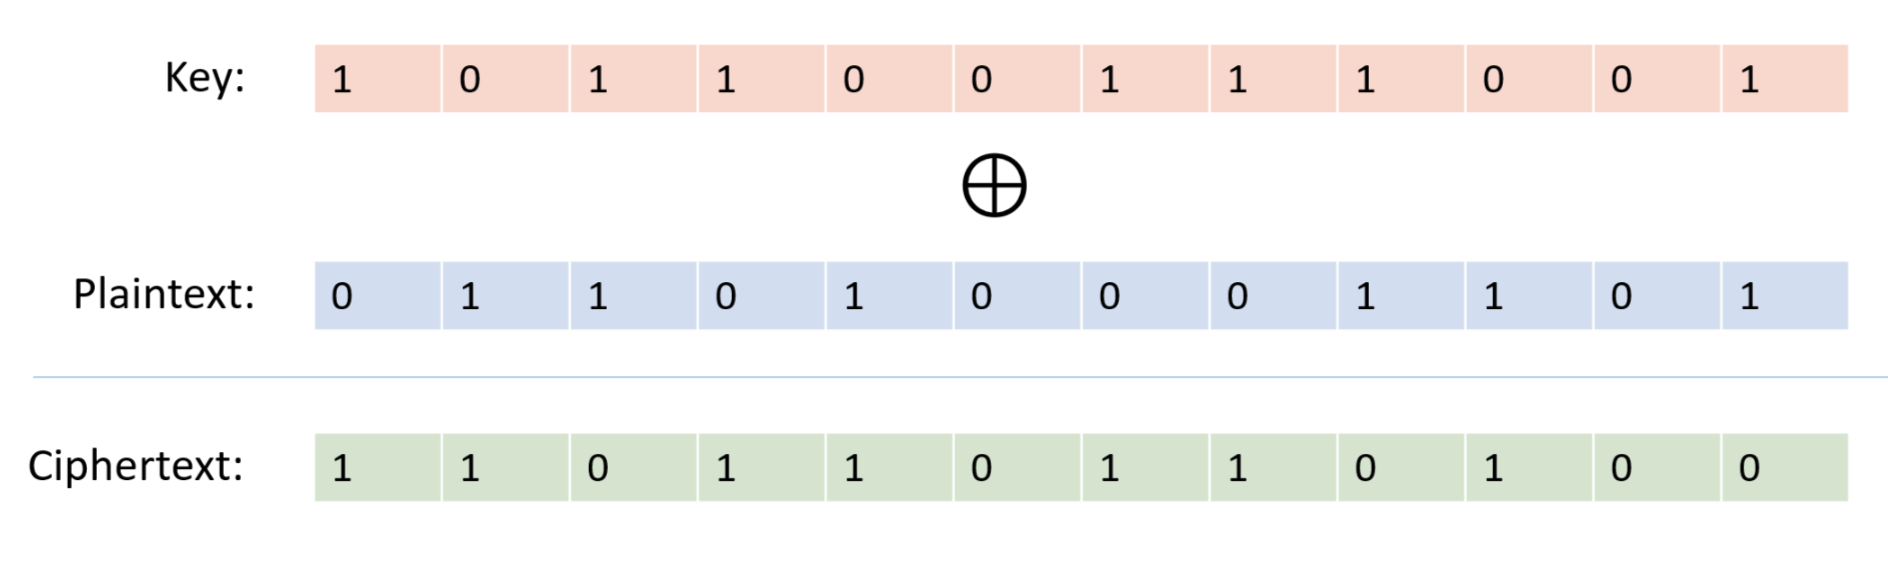
\includegraphics[width=\textwidth, height=0.25\paperheight, keepaspectratio]{../figure/onetimepad.png}
\caption{In the \emph{one time pad} encryption scheme we encrypt a
plaintext \(m\in \{0,1\}^n\) with a key \(k\in \{0,1\}^n\) by the
ciphertext \(m \oplus k\) where \(\oplus\) denotes the bitwise XOR
operation.}
\label{onetimepadfig}
\end{figure}

\begin{proof}[Proof of \cref{onetimepad}] \label[proof]{1-For-two-binary-strings}

For two binary strings \(a\) and \(b\) of the same length \(n\), we
define \(a \oplus b\) to be the string \(c \in \{0,1\}^n\) such that
\(c_i = a_i + b_i \mod 2\) for every \(i\in [n]\). The encryption scheme
\((E,D)\) is defined as follows: \(E_k(m) = m\oplus k\) and
\(D_k(c)= c \oplus k\). By the associative law of addition (which works
also modulo two),
\(D_k(E_k(m))=(m\oplus k) \oplus k = m \oplus (k \oplus k) = m \oplus 0^n = m\),
using the fact that for every bit \(\sigma \in \{0,1\}\),
\(\sigma + \sigma \mod 2 = 0\) and \(\sigma + 0 = \sigma \mod 2\). Hence
\((E,D)\) form a valid encryption.

To analyze the perfect secrecy property, we claim that for every
\(m\in \{0,1\}^n\), the distribution \(Y_m=E_k(m)\) where
\(k \leftarrow_R \{0,1\}^n\) is simply the uniform distribution over
\(\{0,1\}^n\), and hence in particular the distributions \(Y_{m}\) and
\(Y_{m'}\) are identical for every \(m,m' \in \{0,1\}^n\). Indeed, for
every particular \(y\in \{0,1\}^n\), the value \(y\) is output by
\(Y_m\) if and only if \(y = m \oplus k\) which holds if and only if
\(k= m \oplus y\). Since \(k\) is chosen uniformly at random in
\(\{0,1\}^n\), the probability that \(k\) happens to equal
\(m \oplus y\) is exactly \(2^{-n}\), which means that every string
\(y\) is output by \(Y_m\) with probability \(2^{-n}\).

\end{proof}

\begin{figure}
\centering
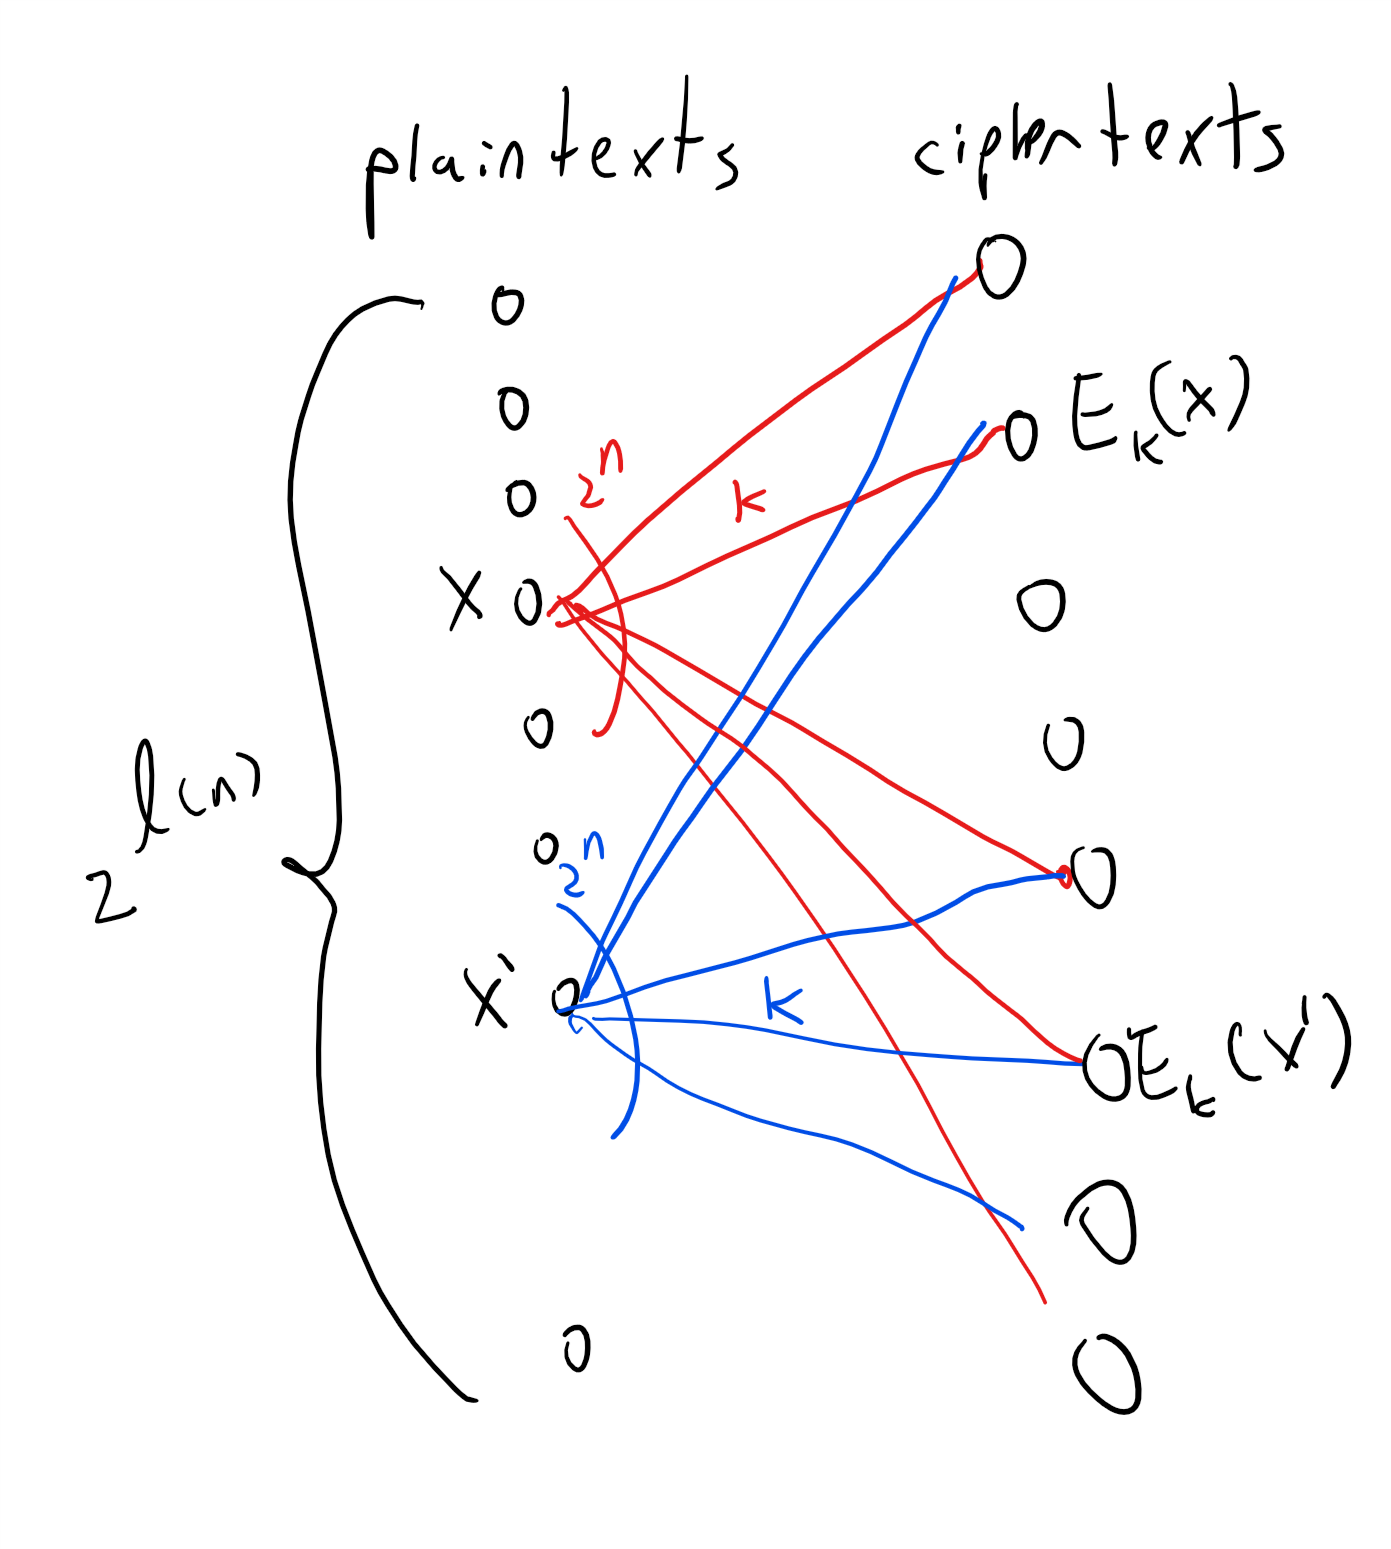
\includegraphics[width=\textwidth, height=0.25\paperheight, keepaspectratio]{../figure/perfectsecrecy.png}
\caption{For any key length \(n\), we can visualize an encryption scheme
\((E,D)\) as a graph with a vertex for every one of the \(2^{\ell(n)}\)
possible plaintexts and for every one of the ciphertexts in
\(\{0,1\}^*\) of the form \(E_k(x)\) for \(k\in \{0,1\}^n\) and
\(x\in \{0,1\}^{\ell(n)}\). For every plaintext \(x\) and key \(k\), we
add an edge labeled \(k\) between \(x\) and \(E_k(x)\). By the validity
condition, if we pick any fixed key \(k\), the map \(x \mapsto E_k(x)\)
must be one-to-one. The condition of perfect secrecy simply corresponds
to requiring that every two plaintexts \(x\) and \(x'\) have exactly the
same set of neighbors (or multi-set, if there are parallel edges).}
\label{perfectsecfig}
\end{figure}

\begin{pause} \label[pause]{1-The-argument-above-is-}

The argument above is quite simple but is worth reading again. To
understand why the one-time pad is perfectly secret, it is useful to
envision it as a bipartite graph as we've done in
\cref{onetimepadtwofig}. (In fact the encryption scheme of
\cref{onetimepadtwofig} is precisely the one-time pad for \(n=2\).) For
every \(n\), the one-time pad encryption scheme corresponds to a
bipartite graph with \(2^n\) vertices on the ``left side'' corresponding
to the plaintexts in \(\{0,1\}^n\) and \(2^n\) vertices on the ``right
side'' corresponding to the ciphertexts \(\{0,1\}^n\). For every
\(x\in \{0,1\}^n\) and \(k\in \{0,1\}^n\), we connect \(x\) to the
vertex \(y=E_k(x)\) with an edge that we label with \(k\). One can see
that this is the complete bipartite graph, where every vertex on the
left is connected to \emph{all} vertices on the right. In particular
this means that for every left vertex \(x\), the distribution on the
ciphertexts obtained by taking a random \(k\in \{0,1\}^n\) and going to
the neighbor of \(x\) on the edge labeled \(k\) is the uniform
distribution over \(\{0,1\}^n\). This ensures the perfect secrecy
condition.

\end{pause}

\section{Necessity of long keys}\label{1-Necessity-of-long-keys}

So, does \cref{onetimepad} give the final word on cryptography, and
means that we can all communicate with perfect secrecy and live happily
ever after? No it doesn't. While the one-time pad is efficient, and
gives perfect secrecy, it has one glaring disadvantage: to communicate
\(n\) bits you need to store a key of length \(n\). In contrast,
practically used cryptosystems such as AES-128 have a short key of
\(128\) bits (i.e., \(16\) bytes) that can be used to protect terabytes
or more of communication! Imagine that we all needed to use the one time
pad. If that was the case, then if you had to communicate with \(m\)
people, you would have to maintain (securely!) \(m\) huge files that are
each as long as the length of the maximum total communication you expect
with that person. Imagine that every time you opened an account with
Amazon, Google, or any other service, they would need to send you in the
mail (ideally with a secure courier) a DVD full of random numbers, and
every time you suspected a virus, you'd need to ask all these services
for a fresh DVD. This doesn't sound so appealing.

This is not just a theoretical issue. The Soviets have used the one-time
pad for their confidential communication since before the 1940's. In
fact, even before Shannon's work, the U.S. intelligence already knew in
1941 that the one-time pad is in principle ``unbreakable'' (see page 32
in the \href{http://nsarchive.gwu.edu/NSAEBB/NSAEBB278/01.PDF}{Venona
document}). However, it turned out that the hassle of manufacturing so
many keys for all the communication took its toll on the Soviets and
they ended up reusing the same keys for more than one message. They did
try to use them for completely different receivers in the (false) hope
that this wouldn't be detected. The
\href{https://en.wikipedia.org/wiki/Venona_project}{Venona Project} of
the U.S. Army was founded in February 1943 by Gene Grabeel (see
\cref{genegrabeelfig}), a former home economics teacher from Madison
Heights, Virginia and Lt. Leonard Zubko. In October 1943, they had their
breakthrough when it was discovered that the Russians were reusing their
keys. In the 37 years of its existence, the project has resulted in a
treasure chest of intelligence, exposing hundreds of KGB agents and
Russian spies in the U.S. and other countries, including Julius
Rosenberg, Harry Gold, Klaus Fuchs, Alger Hiss, Harry Dexter White and
many others.

\begin{marginfigure}
\centering
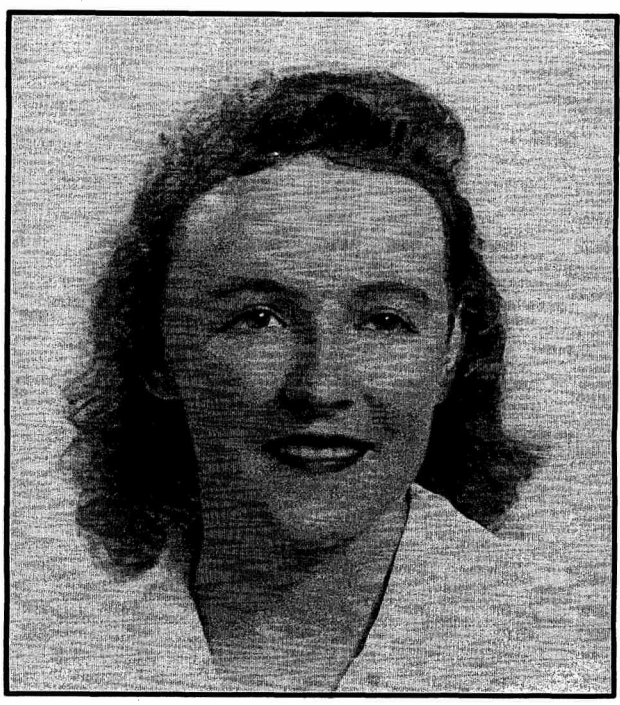
\includegraphics[width=\linewidth, height=1.5in, keepaspectratio]{../figure/genevenona.png}
\caption{Gene Grabeel, who founded the U.S. Russian SigInt program on 1
Feb 1943. Photo taken in 1942, see Page 7 in the Venona historical
study.}
\label{genegrabeelfig}
\end{marginfigure}

\begin{marginfigure}
\centering
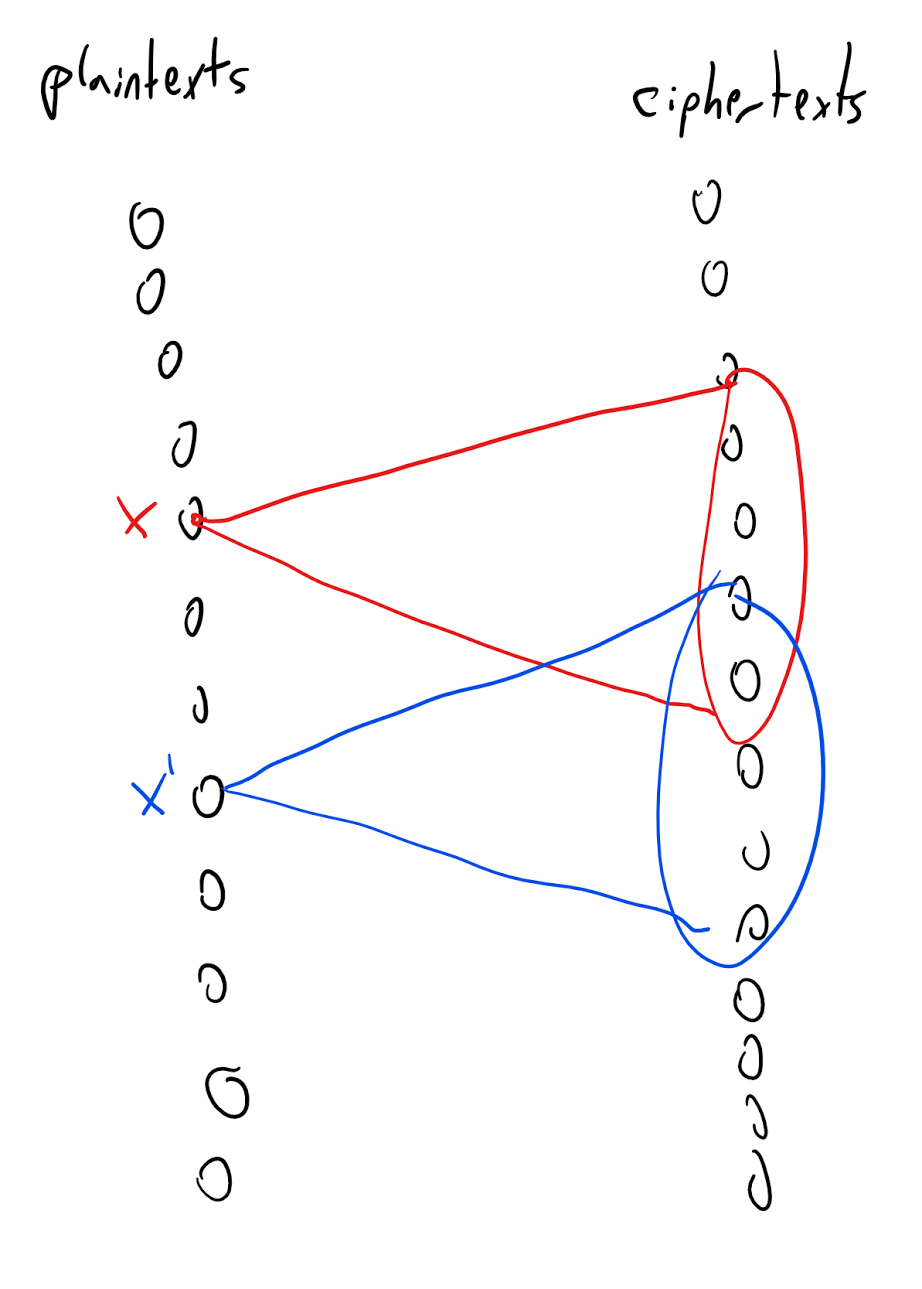
\includegraphics[width=\linewidth, height=1.5in, keepaspectratio]{../figure/longkeygraph.png}
\caption{An encryption scheme where the number of keys is smaller than
the number of plaintexts corresponds to a bipartite graph where the
degree is smaller than the number of vertices on the left side. Together
with the validity condition this implies that there will be two left
vertices \(x,x'\) with non-identical neighborhoods, and hence the scheme
does \emph{not} satisfy perfect secrecy.}
\label{longkeygraphfig}
\end{marginfigure}

Unfortunately it turns out that that such long keys are \emph{necessary}
for perfect secrecy:

\hypertarget{longkeysthm}{}
\begin{theorem}[Perfect secrecy requires long keys] \label[theorem]{longkeysthm}

For every perfectly secret encryption scheme \((E,D)\) the length
function \(\ell\) satisfies \(\ell(n) \leq n\).

\end{theorem}

\begin{proofidea} \label[proofidea]{1-The-idea-behind-the-pr}

The idea behind the proof is illustrated in \cref{longkeygraphfig}. We
define a graph between the plaintexts and ciphertexts, where we put an
edge between plaintext \(x\) and ciphertext \(y\) if there is some key
\(k\) such that \(y=E_k(x)\). The \emph{degree} of this graph is at most
the number of potential keys. The fact that the degree is smaller than
the number of plaintexts (and hence of ciphertexts) implies that there
would be two plaintexts \(x\) and \(x'\) with different sets of
neighbors, and hence the distribution of a ciphertext corresponding to
\(x\) (with a random key) will not be identical to the distribution of a
ciphertext corresponding to \(x'\).

\end{proofidea}

\begin{proof}[Proof of \cref{longkeysthm}] \label[proof]{1-Let-ED-be-a-valid-encr}

Let \(E,D\) be a valid encryption scheme with messages of length
\(\ell\) and key of length \(n<\ell\). We will show that \((E,D)\) is
not perfectly secret by providing two plaintexts
\(x_0,x_1 \in \{0,1\}^\ell\) such that the distributions \(Y_{x_0}\) and
\(Y_{x_1}\) are not identical, where \(Y_x\) is the distribution
obtained by picking \(k \leftarrow_R \{0,1\}^n\) and outputting
\(E_k(x)\).

We choose \(x_0 = 0^\ell\). Let \(S_0 \subseteq \{0,1\}^*\) be the set
of all ciphertexts that have nonzero probability of being output in
\(Y_{x_0}\). That is,
\(S_0=\{ y \;|\; \exists_{k\in \{0,1\}^n} y=E_k(x_0) \}\). Since there
are only \(2^n\) keys, we know that \(|S_0| \leq 2^n\).

We will show the following claim:

\textbf{Claim I:} There exists some \(x_1 \in \{0,1\}^\ell\) and
\(k\in \{0,1\}^n\) such that \(E_k(x_1) \not\in S_0\).

Claim I implies that the string \(E_k(x_1)\) has positive probability of
being output by \(Y_{x_1}\) and zero probability of being output by
\(Y_{x_0}\) and hence in particular \(Y_{x_0}\) and \(Y_{x_1}\) are not
identical. To prove Claim I, just choose a fixed \(k\in \{0,1\}^n\). By
the validity condition, the map \(x \mapsto E_k(x)\) is a one to one map
of \(\{0,1\}^\ell\) to \(\{0,1\}^*\) and hence in particular the
\emph{image} of this map which is the set
\(I_k = \{ y \;|\; \exists_{x\in \{0,1\}^\ell} y=E_k(x) \}\) has size at
least (in fact exactly) \(2^\ell\). Since \(|S_0| \leq 2^n < 2^\ell\),
this means that \(|I_k|>|S_0|\) and so in particular there exists some
string \(y\) in \(I_k \setminus S_0\). But by the definition of \(I_k\)
this means that there is some \(x\in \{0,1\}^\ell\) such that
\(E_k(x) \not\in S_0\) which concludes the proof of Claim I and hence of
\cref{longkeysthm}.

\end{proof}

\hypertarget{addingprobrem}{}
\begin{remark}[Adding probability into the picture] \label[remark]{addingprobrem}

There is a sense in which both our secrecy and our impossibility results
might not be fully convincing, and that is that we did not explicitly
consider algorithms that use \emph{randomness} . For example, maybe Eve
can break a perfectly secret encryption if she is not modeled as a
deterministic function \(Eve:\{0,1\}^o\rightarrow\{0,1\}^\ell\) but
rather a \emph{probabilistic} process. Similarly, maybe the encryption
and decryption functions could be probabilistic processes as well. It
turns out that none of those matter.

For the former, note that a probabilistic process can be thought of as a
\emph{distribution} over functions, in the sense that we have a
collection of functions \(f_1,...,f_N\) mapping \(\{0,1\}^o\) to
\(\{0,1\}^\ell\), and some probabilities \(p_1,\ldots,p_N\)
(non-negative numbers summing to \(1\)), so we now think of Eve as
selecting the function \(f_i\) with probability \(p_i\). But if none of
those functions can give an advantage better than \(1/2\), then neither
can this collection (this is related to the \emph{averaging principle}
in probability).

A similar (though more involved) argument shows that the impossibility
result showing that the key must be at least as long as the message
still holds even if the encryption and decryption algorithms are allowed
to be probabilistic processes as well (working this out is a great
exercise).

\end{remark}

\subsection{Amplifying success
probability}\label{1-Amplifying-success-pro}

\cref{longkeysthm} implies that for every encryption scheme \((E,D)\)
with \(\ell(n)>n\), there is a pair of messages \(x_0,x_1\) and an
attacker \(Eve\) that can distinguish between an encryption of \(x_0\)
and an encryption of \(x_1\) with success better than \(1/2\). But
perhaps Eve's success is only marginally better than half, say
\(0.50001\)? It turns out that's not the case. If the message is even
somewhat larger than the key, the success of Eve can be very close to
\(1\):

\hypertarget{longkeyhighprob}{}
\begin{theorem}[Short keys imply high probability attack] \label[theorem]{longkeyhighprob}

Let \((E,D)\) be an encryption scheme with \(\ell(n)=n+t\). Then there
is a function \(Eve\) and pair of messages \(x_0,x_1\) such that
\begin{equation*}
\Pr_{k \leftarrow_R \{0,1\}^n, b \leftarrow_R \{0,1\}}[ Eve(E_k(x_b)) = x_b] \geq 1- 2^{-t-1}\;.
\end{equation*}

\end{theorem}

\begin{proof} \label[proof]{1-As-in-the-proof-of-cre}

As in the proof of \cref{longkeysthm}, let \(\ell=\ell(n)\) and let
\(x_0 = 0^\ell\) and \(S_0 = \{ E_k(x_0) : k\in \{0,1\}^n \}\) be the
set of size at most \(2^n\) of all ciphertexts corresponding to \(x_0\).
We claim that

\[\Pr_{k \leftarrow_R \{0,1\}^n , x \in \{0,1\}^\ell}[ E_k(x) \in S_0 ] \leq 2^{-t}\;. \label{eqlongkeyprobproof}\]

We show this by arguing that this bound holds for every fixed \(k\),
when we take the probability over \(x\), and so in particular it holds
also for random \(k\). Indeed, for every fixed \(k\), the map
\(x \mapsto E_k(x)\) is a one-to-one map, and so the distribution of
\(E_k(x)\) for random \(x\in \{0,1\}^\ell\) is uniform over some set
\(T_k\) of size \(2^{n+t}\). For every \(k\), the probability over \(x\)
that \(E_k(x) \in S_0\) is equal to
\begin{equation*}
\tfrac{|T_k \cap S_0|}{|T_k|} \leq \tfrac{|S_0|}{|T_k|} \leq \tfrac{2^n}{2^{n+t}}=2^{-t}
\end{equation*}
thus proving \eqref{eqlongkeyprobproof}.

Now, for every \(x\), define \(p_x\) to be
\(\Pr_{k \leftarrow_R \{0,1\}^n}[ E_k(x) \in S_0]\). By
\eqref{eqlongkeyprobproof}, the expectation of \(p_x\) over random
\(x \leftarrow_R \{0,1\}^n\) is at most \(2^{-t}\) and so in particular
by the averaging argument \emph{there exists} some \(x_1\) such that
\(p_{x_1} \leq 2^{-t}\). Yet that means that the following adversary
\(Eve\) will be able to distinguish between an encryption of \(x_0\) and
an encryption of \(x_1\) with probability at least \(1-2^{-t-1}\):

\begin{itemize}
\item
  \textbf{Input:} A ciphertext \(y\in \{0,1\}^*\)
\item
  \textbf{Operation:} If \(y\in S_0\), output \(x_0\), otherwise output
  \(x_1\).
\end{itemize}

The probability that \(Eve(E_k(x_0))=x_0\) is equal to \(1\), while the
probability that \(Eve(E_k(x_1))=x_1\) is equal to
\(1-p_{x_1} \geq 1- 2^{-t}\). Hence the overall probability of \(Eve\)
guessing correctly is

\begin{equation*}
\tfrac{1}{2} \cdot 1 + \tfrac{1}{2} \cdot \left( 1-2^{-t} \right) = 1 - 2^{-t-1} \;.
\end{equation*}

\end{proof}

\section{Bibliographical notes}\label{1-Bibliographical-notes}

Much of this text is shared with \href{https://introtcs.org}{my
Introduction to Theoretical Computer Science textbook}.

Shannon's manuscript was written in 1945 but was classified, and a
partial version was only published in 1949. Still it has revolutionized
cryptography, and is the forerunner to much of what followed.

The Venona project's history is described in
\href{http://nsarchive.gwu.edu/NSAEBB/NSAEBB278/01.PDF}{this document}.
Aside from Grabeel and Zubko, credit to the discovery that the Soviets
were reusing keys is shared by Lt. Richard Hallock, Carrie Berry, Frank
Lewis, and Lt. Karl Elmquist, and there are others that have made
important contributions to this project. See pages 27 and 28 in the
document.

In a
\href{https://www.nsa.gov/news-features/declassified-documents/nash-letters/assets/files/nash_letters1.pdf}{1955
letter to the NSA} that only recently came forward, John Nash proposed
an ``unbreakable'' encryption scheme. He wrote \emph{``I hope my
handwriting, etc. do not give the impression I am just a crank or
circle-squarer\ldots{} The significance of this conjecture {[}that
certain encryption schemes are exponentially secure against key recovery
attacks{]} .. is that it is quite feasible to design ciphers that are
effectively unbreakable.''} John Nash made seminal contributions in
mathematics and game theory, and was awarded both the Abel Prize in
mathematics and the Nobel Memorial Prize in Economic Sciences. However,
he has struggled with mental illness throughout his life. His biography,
\href{https://en.wikipedia.org/wiki/A_Beautiful_Mind_(book)}{A Beautiful
Mind} was made into a popular movie. It is natural to compare Nash's
1955 letter to the NSA to the 1956 letter by
\href{https://www.cs.cmu.edu/~aada/courses/15251s15/www/notes/godel-letter.pdf}{Kurt
Gödel to John von Neumann}. From the theoretical computer science point
of view, the crucial difference is that while Nash informally talks
about exponential vs polynomial computation time, he does not mention
the word ``Turing Machine'' or other models of computation, and it is
not clear if he is aware or not that his conjecture can be made
mathematically precise (assuming a formalization of ``sufficiently
complex types of enciphering'').



\chapter{Mathematical Background}\label{chapmath}

\begin{objectives} \label[objectives]{Recall-basic-mathematical}

\begin{itemize}
\tightlist
\item
  Recall basic mathematical notions such as sets, functions, numbers,
  logical operators and quantifiers, strings, and graphs.
\item
  Rigorously define Big-\(O\) notation.
\item
  Proofs by induction.
\item
  Practice with reading mathematical \emph{definitions},
  \emph{statements}, and \emph{proofs}.
\item
  Transform an intuitive argument into a rigorous proof.
\end{itemize}

\end{objectives}

\begin{quote}
\emph{``I found that every number, which may be expressed from one to
ten, surpasses the preceding by one unit: afterwards the ten is doubled
or tripled \ldots{} until a hundred; then the hundred is doubled and
tripled in the same manner as the units and the tens \ldots{} and so
forth to the utmost limit of numeration.''}, Muhammad ibn Mūsā
al-Khwārizmī, 820, translation by Fredric Rosen, 1831.
\end{quote}

In this chapter we review some of the mathematical concepts that we use
in this book. These concepts are typically covered in courses or
textbooks on ``mathematics for computer science'' or ``discrete
mathematics''; see the ``Bibliographical Notes'' section
(\cref{notesmathchap}) for several excellent resources on these topics
that are freely-available online.

\emph{A mathematician's apology.} Some students might wonder why this
book contains so much math. Mathematics is a language for modeling
concepts in a precise and unambiguous way. In this book we use math to
model the concept of \emph{computation}. For example, we will consider
questions such as \emph{``is there an efficient algorithm to find the
prime factors of a given integer?''}. (We will see that this question is
particularly interesting, touching on areas as far apart as Internet
security and quantum mechanics!) To even \emph{phrase} such a question,
we need to give a precise \emph{definition} of the notion of an
\emph{algorithm}, and of what it means for an algorithm to be
\emph{efficient}. Also, since there is no empirical experiment that will
prove the \emph{nonexistence} of an algorithm, the only way to establish
such a result is using a \emph{mathematical proof}.

\section{This chapter: a reader's manual}\label{manualbackground}

Depending on your background, you can approach this chapter in two
different ways:

\begin{itemize}
\item
  If you already have taken a ``discrete mathematics'', ``mathematics
  for computer science'' or similar courses, you can take a quick look
  at \cref{secmathoverview} to see the main tools we will use,
  \cref{notationsec} for our notation and conventions, and then skip
  ahead to the rest of this book. Alternatively, you can sit back,
  relax, and read this chapter just to get familiar with our notation,
  as well as to enjoy (or not) my philosophical musings and attempts at
  humor. You might also want to start brushing up on \emph{discrete
  probability}, which we'll use later in this book.
\item
  If your background is less extensive, see \cref{notesmathchap} for
  some resources on these topics. This chapter briefly covers the
  concepts that we need, but you may find it helpful to see a more
  in-depth treatment. As usual with math, the best way to get comfort
  with this material is to work out exercises on your own.
\end{itemize}

\section{A quick overview of mathematical
prerequisites}\label{secmathoverview}

The main mathematical concepts we use in this book are:

\begin{itemize}
\item
  \textbf{Proofs:} First and foremost, this book involves a heavy dose
  of formal mathematical reasoning, which includes mathematical
  \emph{definitions}, \emph{statements}, and \emph{proofs}.
\item
  \textbf{Sets:} The basic set \emph{relations} of membership (\(\in\))
  and containment (\(\subseteq\)), and set \emph{operations},
  principally union (\(\cup\)), intersection (\(\cap\)), set difference
  (\(\setminus\)) and Cartesian product (\(\times\)).
\item
  \textbf{Tuples and strings:} The set \(\Sigma^k\) of length-\(k\)
  strings/lists over elements in \(\Sigma\), where \(\Sigma\) is some
  finite set which is called the \emph{alphabet} (quite often
  \(\Sigma = \{0,1\}\)). We use \(\Sigma^*\) for the set of all strings
  of finite length.
\item
  \textbf{Some special sets:} The set \(\N\) of natural numbers.
  Following typical computer science convention, our indices start from
  zero and so we write \(\N = \{0,1,2,\ldots \}\). We use \([n]\) for
  the set \(\{0,1,2,\ldots,n-1\}\). We use \(\{0,1\}^*\) for the set of
  all binary strings and \(\{0,1\}^n\) for the set of strings of length
  \(n\) for some natural number \(n\in\N\). If \(x\) is a string of
  length \(n\), then we refer to its elements by \(x_0,\ldots,x_{n-1}\).
\item
  \textbf{Functions:} The \emph{domain} and \emph{codomain} of a
  function, properties such as being \emph{one-to-one} (also known as
  \emph{injective}) or \emph{onto} (also known as \emph{surjective})
  functions, as well as \emph{partial functions} (that, unlike standard
  or ``total'' functions, are not necessarily defined on all elements of
  their domain).
\item
  \textbf{Logical operations:} The operations AND (\(\wedge\)), OR
  (\(\vee\)), and NOT (\(\neg\)) and the quantifiers ``there exists''
  (\(\exists\)) and ``for all'' (\(\forall\)).
\item
  \textbf{Basic combinatorics:} Notions such as \(\binom{n}{k}\) (the
  number of \(k\)-sized subsets of a set of size \(n\)).
\item
  \textbf{Graphs:} Undirected and directed graphs, connectivity, paths,
  and cycles.
\item
  \textbf{Big-\(O\) notation:} \(O,o,\Omega,\omega,\Theta\) notation for
  analyzing asymptotic growth of functions.
\item
  \textbf{Discrete probability:} We will use \emph{probability theory},
  and specifically probability over \emph{finite} samples spaces such as
  tossing \(n\) coins, including notions such as \emph{random
  variables}, \emph{expectation}, and \emph{concentration}. We will only
  use probability theory in the second half of this text, and will
  review it beforehand. However, probabilistic reasoning is a subtle
  (and extremely useful!) skill, and it's always good to start early in
  acquiring it.
\end{itemize}

In the rest of this chapter we briefly review the above notions. This is
partially to remind the reader and reinforce material that might not be
fresh in your mind, and partially to introduce our notation and
conventions which might occasionally differ from those you've
encountered before.

\section{Reading mathematical texts}\label{Reading-mathematical-text}

Reading mathematical texts take practice to get used to the notation and
symbols. Mathematicians use jargon for the same reason that it is used
in many other professions such engineering, law, medicine, and others.
We want to make terms \emph{precise} and introduce shorthand for
concepts that are frequently reused. Mathematical texts tend to ``pack a
lot of punch'' per sentence, and so the key is to read them slowly and
carefully, parsing each symbol at a time.

With time and practice you will see that reading mathematical texts
becomes easier and jargon is no longer an issue. Moreover, reading
mathematical texts is one of the most transferable skills you could take
from this book. Our world is changing rapidly, not just in the realm of
technology, but also in many other human endeavors, whether it is
medicine, economics, law or even culture. Whatever your future
aspirations, it is likely that you will encounter texts that use new
concepts that you have not seen before (see \cref{alphagozerofig} and
\cref{zerocashfig} for two recent examples from current ``hot areas'').
Being able to internalize and then apply new definitions can be hugely
important. It is a skill that's much easier to acquire in the relatively
safe and stable context of a mathematical course, where one at least has
the guarantee that the concepts are fully specified, and you have access
to your teaching staff for questions.


\begin{marginfigure}
\centering
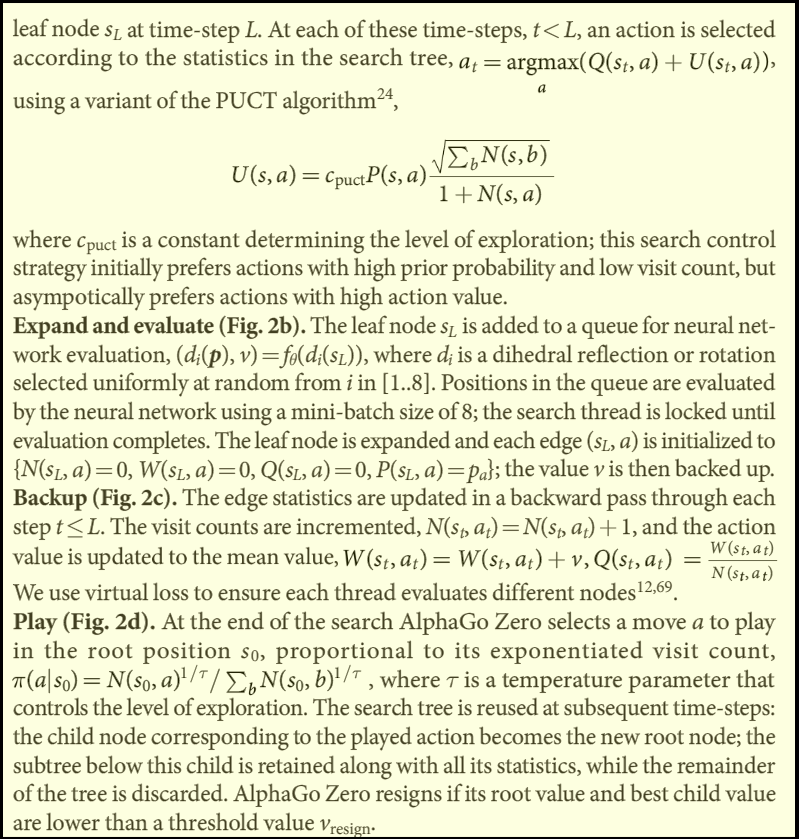
\includegraphics[width=\linewidth, height=1.5in, keepaspectratio]{../figure/alphagozero.png}
\caption{A snippet from the ``methods'' section of the
\href{https://goo.gl/k8pVpL}{``AlphaGo Zero'' paper} by Silver et al,
\emph{Nature}, 2017.}
\label{alphagozerofig}
\end{marginfigure}


\begin{marginfigure}
\centering
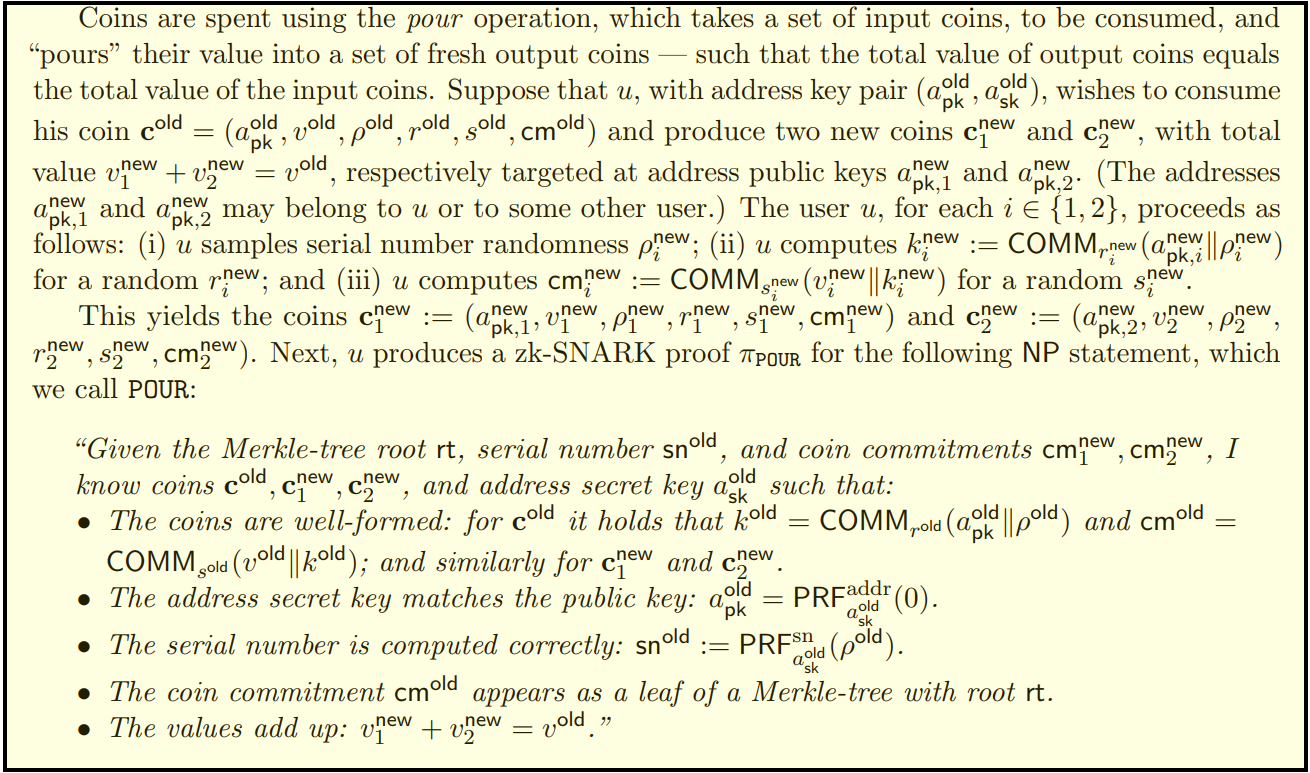
\includegraphics[width=\linewidth, height=1.5in, keepaspectratio]{../figure/zerocash.png}
\caption{A snippet from the
\href{http://zerocash-project.org/paper}{``Zerocash'' paper} of
Ben-Sasson et al, that forms the basis of the cryptocurrency startup
Zcash.}
\label{zerocashfig}
\end{marginfigure}

The basic components of a mathematical text are \textbf{definitions},
\textbf{assertions} and \textbf{proofs}.

\subsection{Definitions}\label{Definitions}

Mathematicians often define new concepts in terms of old concepts.\\
Here is a mathematical definition which you may have encountered in the
past (and will see again shortly):

\hypertarget{onetoonedef}{}
\begin{definition}[One to one function] \label[definition]{onetoonedef}

Let \(S,T\) be sets. We say that a function \(f:S \rightarrow T\) is
\emph{one to one} (also known as \emph{injective}) if for every two
elements \(x,x' \in S\), if \(x \neq x'\) then \(f(x) \neq f(x')\).

\end{definition}

\cref{onetoonedef} captures a simple concept, but even so it uses quite
a bit of notation. When reading such a definition, it is often useful to
annotate it with a pen as you're going through it, as in
\cref{onetoonedefannotatedef}. For example, when you see an identifier
such as \(f\), \(S\) or \(x\), make sure that you realize what sort of
object is it: is it a set, a function, an element, a number, a gremlin?
You might also find it useful to explain the definition in words to a
friend (or to yourself).


\begin{marginfigure}
\centering
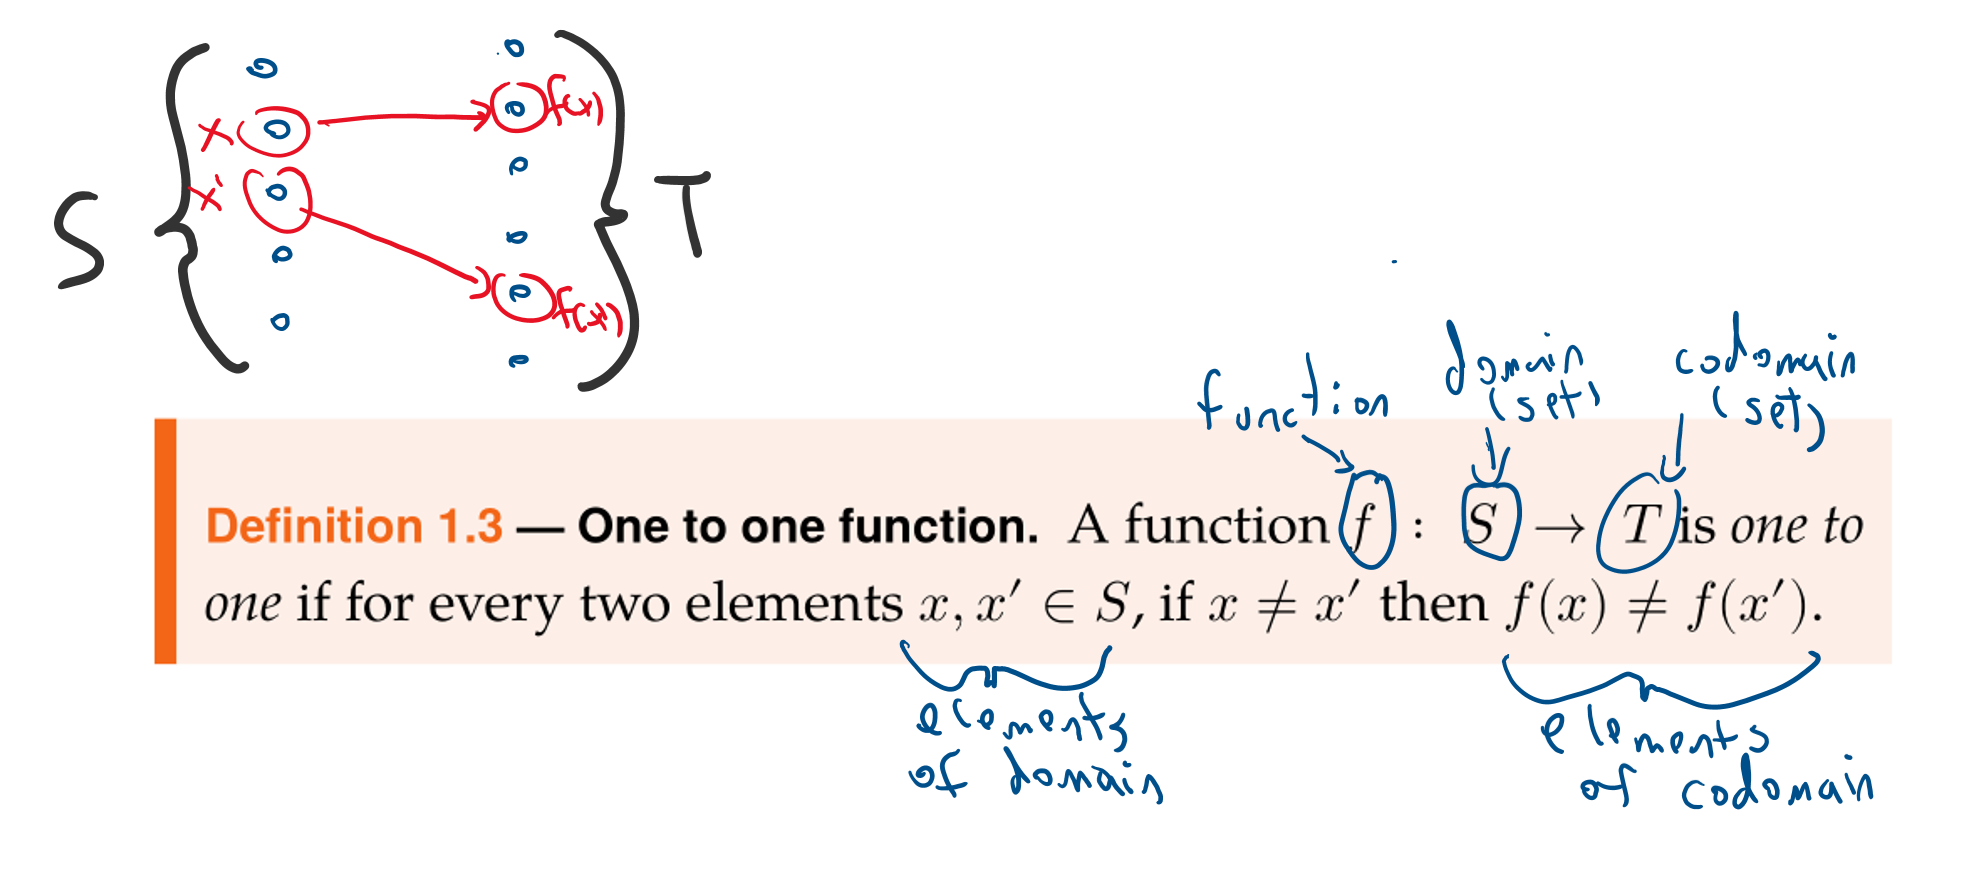
\includegraphics[width=\linewidth, height=1.5in, keepaspectratio]{../figure/onetoonedef.png}
\caption{An annotated form of \cref{onetoonedef}, marking which type is
every object, and with a doodle explaining what the definition says.}
\label{onetoonedefannotatedef}
\end{marginfigure}

\subsection{Assertions: Theorems, lemmas,
claims}\label{Assertions-Theorems-lemma}

Theorems, lemmas, claims and the like are true statements about the
concepts that we defined. Deciding whether to call a particular
statement a ``Theorem'', a ``Lemma'' or a ``Claim'' is a judgement call,
and does not make a mathematical difference. All three correspond to
true statements which can be proven. The difference is that a
\emph{Theorem} refers to a significant result, that we would want to
remember and highlight. A \emph{Lemma} often refers to a technical
result, that is not necessarily important in its own right, but can be
often very useful in proving other theorems. A \emph{Claim} is a ``throw
away'' statement, that we need to use in order to prove some other
bigger results, but do not care so much about for its own sake.

\subsection{Proofs}\label{Proofs}

Mathematical \emph{proofs} are the arguments we use to demonstrate that
our theorems, lemmas, and claims area indeed true. We discuss proofs in
\cref{proofsbackgroundsec} below, but the main point is that the
mathematical standard of proof is very high. Unlike in some other
realms, in mathematics a proof is an ``airtight'' argument that
demonstrates that the statement is true beyond a shadow of a doubt. Some
examples in this section for mathematical proofs are given in
\cref{simplepathlemex} and \cref{topsortsec}. As mentioned in the
preface, as a general rule, it is more important you understand the
\textbf{definitions} than the \textbf{theorems}, and it is more
important you understand a \textbf{theorem statement} than its
\textbf{proof}.

\section{Basic discrete math objects}\label{Basic-discrete-math-objec}

In this section we quickly review some of the mathematical objects (the
``basic data structures'' of mathematics, if you will) we use in this
book.

\subsection{Sets}\label{Sets}

A \emph{set} is an unordered collection of objects. For example, when we
write \(S = \{ 2,4, 7 \}\), we mean that \(S\) denotes the set that
contains the numbers \(2\), \(4\), and \(7\). (We use the notation
``\(2 \in S\)'' to denote that \(2\) is an element of \(S\).) Note that
the set \(\{ 2, 4, 7 \}\) and \(\{ 7 , 4, 2 \}\) are identical, since
they contain the same elements. Also, a set either contains an element
or does not contain it -- there is no notion of containing it ``twice''
-- and so we could even write the same set \(S\) as \(\{ 2, 2, 4, 7\}\)
(though that would be a little weird). The \emph{cardinality} of a
finite set \(S\), denoted by \(|S|\), is the number of elements it
contains. (Cardinality can be defined for \emph{infinite} sets as well;
see the sources in \cref{notesmathchap}.) So, in the example above,
\(|S|=3\). A set \(S\) is a \emph{subset} of a set \(T\), denoted by
\(S \subseteq T\), if every element of \(S\) is also an element of
\(T\). (We can also describe this by saying that \(T\) is a
\emph{superset} of \(S\).) For example,
\(\{2,7\} \subseteq \{ 2,4,7\}\). The set that contains no elements is
known as the \emph{empty set} and it is denoted by \(\emptyset\). If
\(A\) is a subset of \(B\) that is not equal to \(B\) we say that \(A\)
is a \emph{strict subset} of \(B\), and denote this by
\(A \subsetneq B\).

We can define sets by either listing all their elements or by writing
down a rule that they satisfy such as \[
\text{EVEN} = \{ x  \;|\; \text{ $x=2y$ for some non-negative integer $y$} \} \;.
\]

Of course there is more than one way to write the same set, and often we
will use intuitive notation listing a few examples that illustrate the
rule. For example, we can also define \(\text{EVEN}\) as

\[
\text{EVEN} = \{ 0,2,4, \ldots \} \;.
\]

Note that a set can be either finite (such as the set \(\{2,4,7\}\)) or
infinite (such as the set \(\text{EVEN}\)). Also, the elements of a set
don't have to be numbers. We can talk about the sets such as the set
\(\{a,e,i,o,u \}\) of all the vowels in the English language, or the set
\(\{\)\texttt{New York}, \texttt{Los Angeles}, \texttt{Chicago},
\texttt{Houston}, \texttt{Philadelphia}, \texttt{Phoenix},
\texttt{San Antonio}, \texttt{San Diego}, \texttt{Dallas}\(\}\) of all
cities in the U.S. with population more than one million per the 2010
census. A set can even have other sets as elements, such as the set
\(\{ \emptyset, \{1,2\},\{2,3\},\{1,3\} \}\) of all even-sized subsets
of \(\{1,2,3\}\).

\paragraph{Operations on sets:} The \emph{union} of two sets \(S,T\),
denoted by \(S \cup T\), is the set that contains all elements that are
either in \(S\) \emph{or} in \(T\). The \emph{intersection} of \(S\) and
\(T\), denoted by \(S \cap T\), is the set of elements that are both in
\(S\) \emph{and} in \(T\). The \emph{set difference} of \(S\) and \(T\),
denoted by \(S \setminus T\) (and in some texts also by \(S-T\)), is the
set of elements that are in \(S\) but \emph{not} in \(T\).

\paragraph{Tuples, lists, strings, sequences:} A \emph{tuple} is an
\emph{ordered} collection of items. For example \((1,5,2,1)\) is a tuple
with four elements (also known as a \(4\)-tuple or quadruple). Since
order matters, this is not the same tuple as the \(4\)-tuple
\((1,1,5,2)\) or the \(3\)-tuple \((1,5,2)\). A \(2\)-tuple is also
known as a \emph{pair}. We use the terms \emph{tuples} and \emph{lists}
interchangeably. A tuple where every element comes from some finite set
\(\Sigma\) (such as \(\{0,1\}\)) is also known as a \emph{string}.
Analogously to sets, we denote the \emph{length} of a tuple \(T\) by
\(|T|\). Just like sets, we can also think of infinite analogues of
tuples, such as the ordered collection \((1,4,9,\ldots )\) of all
perfect squares. Infinite ordered collections are known as
\emph{sequences}; we might sometimes use the term ``infinite sequence''
to emphasize this, and use ``finite sequence'' as a synonym for a tuple.
(We can identify a sequence \((a_0,a_1,a_2,\ldots)\) of elements in some
set \(S\) with a \emph{function} \(A:\N \rightarrow S\) (where
\(a_n = A(n)\) for every \(n\in \N\)). Similarly, we can identify a
\(k\)-tuple \((a_0,\ldots,a_{k-1})\) of elements in \(S\) with a
function \(A:[k] \rightarrow S\).)

\paragraph{Cartesian product:} If \(S\) and \(T\) are sets, then their
\emph{Cartesian product}, denoted by \(S \times T\), is the set of all
ordered pairs \((s,t)\) where \(s\in S\) and \(t\in T\). For example, if
\(S = \{1,2,3 \}\) and \(T = \{10,12 \}\), then \(S\times T\) contains
the \(6\) elements \((1,10),(2,10),(3,10),(1,12),(2,12),(3,12)\).
Similarly if \(S,T,U\) are sets then \(S\times T \times U\) is the set
of all ordered triples \((s,t,u)\) where \(s\in S\), \(t\in T\), and
\(u\in U\). More generally, for every positive integer \(n\) and sets
\(S_0,\ldots,S_{n-1}\), we denote by
\(S_0 \times S_1 \times \cdots \times S_{n-1}\) the set of ordered
\(n\)-tuples \((s_0,\ldots,s_{n-1})\) where \(s_i\in S_i\) for every
\(i \in \{0,\ldots, n-1\}\). For every set \(S\), we denote the set
\(S\times S\) by \(S^2\), \(S\times S\times S\) by \(S^3\),
\(S\times S\times S \times S\) by \(S^4\), and so on and so forth.

\subsection{Special sets}\label{specialsets}

There are several sets that we will use in this book time and again. The
set

\[
\N = \{ 0, 1,2, \ldots \}
\] contains all \emph{natural numbers}, i.e., non-negative integers. For
any natural number \(n\in\N\), we define the set \([n]\) as
\(\{0,\ldots, n-1\} = \{ k\in \N : k < n \}\). (We start our indexing of
both \(\N\) and \([n]\) from \(0\), while many other texts index those
sets from \(1\). Starting from zero or one is simply a convention that
doesn't make much difference, as long as one is consistent about it.)

We will also occasionally use the set
\(\Z=\{\ldots,-2,-1,0,+1,+2,\ldots \}\) of (negative and non-negative)
\emph{integers},\footnote{The letter Z stands for the German word
  ``Zahlen'', which means \emph{numbers}.} as well as the set \(\R\) of
\emph{real} numbers. (This is the set that includes not just the
integers, but also fractional and irrational numbers; e.g., \(\R\)
contains numbers such as \(+0.5\), \(-\pi\), etc.) We denote by \(\R_+\)
the set \(\{ x\in \R : x > 0 \}\) of \emph{positive} real numbers. This
set is sometimes also denoted as \((0,\infty)\).

\paragraph{Strings:} Another set we will use time and again is

\[
\{0,1\}^n = \{ (x_0,\ldots,x_{n-1}) \;:\; x_0,\ldots,x_{n-1} \in \{0,1\}  \}
\] which is the set of all \(n\)-length binary strings for some natural
number \(n\). That is \(\{0,1\}^n\) is the set of all \(n\)-tuples of
zeroes and ones. This is consistent with our notation above:
\(\{0,1\}^2\) is the Cartesian product \(\{0,1\} \times \{0,1\}\),
\(\{0,1\}^3\) is the product \(\{0,1\} \times \{0,1\} \times \{0,1\}\)
and so on.

We will write the string \((x_0,x_1,\ldots,x_{n-1})\) as simply
\(x_0x_1\cdots x_{n-1}\). For example,

\[
\{0,1\}^3 = \{ 000 , 001, 010 , 011, 100, 101, 110, 111 \} \;.
\]

For every string \(x\in \{0,1\}^n\) and \(i\in [n]\), we write \(x_i\)
for the \(i^{th}\) element of \(x\).

We will also often talk about the set of binary strings of \emph{all}
lengths, which is

\[
\{0,1\}^* = \{ (x_0,\ldots,x_{n-1}) \;:\; n\in\N \;,\;, x_0,\ldots,x_{n-1} \in \{0,1\} \} \;.
\]

Another way to write this set is as \[
\{0,1\}^* = \{0,1\}^0 \cup \{0,1\}^1 \cup \{0,1\}^2 \cup \cdots
\] or more concisely as

\[
\{0,1\}^* = \cup_{n\in\N} \{0,1\}^n \;.
\]

The set \(\{0,1\}^*\) includes the ``string of length \(0\)'' or ``the
empty string'', which we will denote by
\(\ensuremath{\text{\texttt{""}}}\). (In using this notation we follow
the convention of many programming languages. Other texts sometimes use
\(\epsilon\) or \(\lambda\) to denote the empty string.)

\paragraph{Generalizing the star operation:} For every set \(\Sigma\),
we define

\[\Sigma^* = \cup_{n\in \N} \Sigma^n \;.\] For example, if
\(\Sigma = \{a,b,c,d,\ldots,z \}\) then \(\Sigma^*\) denotes the set of
all finite length strings over the alphabet a-z.

\paragraph{Concatenation:} The \emph{concatenation} of two strings
\(x\in \Sigma^n\) and \(y\in \Sigma^m\) is the \((n+m)\)-length string
\(xy\) obtained by writing \(y\) after \(x\). That is, if
\(x \in \{0,1\}^n\) and \(y\in \{0,1\}^m\), then \(xy\) is equal to the
string \(z\in \{0,1\}^{n+m}\) such that for \(i\in [n]\), \(z_i=x_i\)
and for \(i\in \{n,\ldots,n+m-1\}\), \(z_i = y_{i-n}\).

\subsection{Functions}\label{functionsec}

If \(S\) and \(T\) are nonempty sets, a \emph{function} \(F\) mapping
\(S\) to \(T\), denoted by \(F:S \rightarrow T\), associates with every
element \(x\in S\) an element \(F(x)\in T\). The set \(S\) is known as
the \emph{domain} of \(F\) and the set \(T\) is known as the
\emph{codomain} of \(F\). The \emph{image} of a function \(F\) is the
set \(\{ F(x) \;|\; x\in S\}\) which is the subset of \(F\)'s codomain
consisting of all output elements that are mapped from some input. (Some
texts use \emph{range} to denote the image of a function, while other
texts use \emph{range} to denote the codomain of a function. Hence we
will avoid using the term ``range'' altogether.) As in the case of sets,
we can write a function either by listing the table of all the values it
gives for elements in \(S\) or by using a rule. For example if
\(S = \{0,1,2,3,4,5,6,7,8,9 \}\) and \(T = \{0,1 \}\), then the table
below defines a function \(F: S \rightarrow T\). Note that this function
is the same as the function defined by the rule
\(F(x)= (x \mod 2)\).\footnote{For two natural numbers \(x\) and \(a\),
  \(x \mod a\) (shorthand for \href{https://goo.gl/b7Fdzm}{``modulo''})
  denotes the \emph{remainder} of \(x\) when it is divided by \(a\).
  That is, it is the number \(r\) in \(\{0,\ldots,a-1\}\) such that
  \(x = ak +r\) for some integer \(k\). We sometimes also use the
  notation \(x = y\; (\mod a)\) to denote the assertion that
  \(x \mod a\) is the same as \(y \mod a\).}

\begin{longtable}[]{@{}ll@{}}
\caption{An example of a function.}\tabularnewline
\toprule
Input & Output\tabularnewline
\midrule
\endfirsthead
\toprule
Input & Output\tabularnewline
\midrule
\endhead
0 & 0\tabularnewline
1 & 1\tabularnewline
2 & 0\tabularnewline
3 & 1\tabularnewline
4 & 0\tabularnewline
5 & 1\tabularnewline
6 & 0\tabularnewline
7 & 1\tabularnewline
8 & 0\tabularnewline
9 & 1\tabularnewline
\bottomrule
\end{longtable}

If \(f:S \rightarrow T\) satisfies that \(f(x)\neq f(y)\) for all
\(x \neq y\) then we say that \(f\) is \emph{one-to-one}
(\cref{onetoonedef}, also known as an \emph{injective} function or
simply an \emph{injection}). If \(F\) satisfies that for every
\(y\in T\) there is some \(x\in S\) such that \(F(x)=y\) then we say
that \(F\) is \emph{onto} (also known as a \emph{surjective} function or
simply a \emph{surjection}). A function that is both one-to-one and onto
is known as a \emph{bijective} function or simply a \emph{bijection}. A
bijection from a set \(S\) to itself is also known as a
\emph{permutation} of \(S\). If \(F:S \rightarrow T\) is a bijection
then for every \(y\in T\) there is a unique \(x\in S\) such that
\(F(x)=y\). We denote this value \(x\) by \(F^{-1}(y)\). Note that
\(F^{-1}\) is itself a bijection from \(T\) to \(S\) (can you see why?).

Giving a bijection between two sets is often a good way to show they
have the same size. In fact, the standard mathematical definition of the
notion that ``\(S\) and \(T\) have the same cardinality'' is that there
exists a bijection \(f:S \rightarrow T\). Further, the cardinality of a
set \(S\) is defined to be \(n\) if there is a bijection from \(S\) to
the set \(\{0,\ldots,n-1\}\). As we will see later in this book, this is
a definition that generalizes to defining the cardinality of
\emph{infinite} sets.

\paragraph{Partial functions:} We will sometimes be interested in
\emph{partial} functions from \(S\) to \(T\). A partial function is
allowed to be undefined on some subset of \(S\). That is, if \(F\) is a
partial function from \(S\) to \(T\), then for every \(s\in S\), either
there is (as in the case of standard functions) an element \(F(s)\) in
\(T\), or \(F(s)\) is undefined. For example, the partial function
\(F(x)= \sqrt{x}\) is only defined on non-negative real numbers. When we
want to distinguish between partial functions and standard (i.e.,
non-partial) functions, we will call the latter \emph{total} functions.
When we say ``function'' without any qualifier then we mean a
\emph{total} function.

The notion of partial functions is a strict generalization of functions,
and so every function is a partial function, but not every partial
function is a function. (That is, for every nonempty \(S\) and \(T\),
the set of partial functions from \(S\) to \(T\) is a proper superset of
the set of total functions from \(S\) to \(T\).) When we want to
emphasize that a function \(f\) from \(A\) to \(B\) might not be total,
we will write \(f: A \rightarrow_p B\). We can think of a partial
function \(F\) from \(S\) to \(T\) also as a total function from \(S\)
to \(T \cup \{ \bot \}\) where \(\bot\) is a special ``failure symbol''.
So, instead of saying that \(F\) is undefined at \(x\), we can say that
\(F(x)=\bot\).

\paragraph{Basic facts about functions:} Verifying that you can prove
the following results is an excellent way to brush up on functions:

\begin{itemize}
\item
  If \(F:S \rightarrow T\) and \(G:T \rightarrow U\) are one-to-one
  functions, then their \emph{composition} \(H:S \rightarrow U\) defined
  as \(H(s)=G(F(s))\) is also one to one.
\item
  If \(F:S \rightarrow T\) is one to one, then there exists an onto
  function \(G:T \rightarrow S\) such that \(G(F(s))=s\) for every
  \(s\in S\).
\item
  If \(G:T \rightarrow S\) is onto then there exists a one-to-one
  function \(F:S \rightarrow T\) such that \(G(F(s))=s\) for every
  \(s\in S\).
\item
  If \(S\) and \(T\) are finite sets then the following conditions are
  equivalent to one another: \textbf{(a)} \(|S| \leq |T|\), \textbf{(b)}
  there is a one-to-one function \(F:S \rightarrow T\), and \textbf{(c)}
  there is an onto function \(G:T \rightarrow S\). (This is actually
  true even for \emph{infinite} \(S\) and \(T\): in that case
  \textbf{(b)} (or equivalently \textbf{(c)}) is the commonly accepted
  \emph{definition} for \(|S| \leq |T|\).)
\end{itemize}


\begin{marginfigure}
\centering
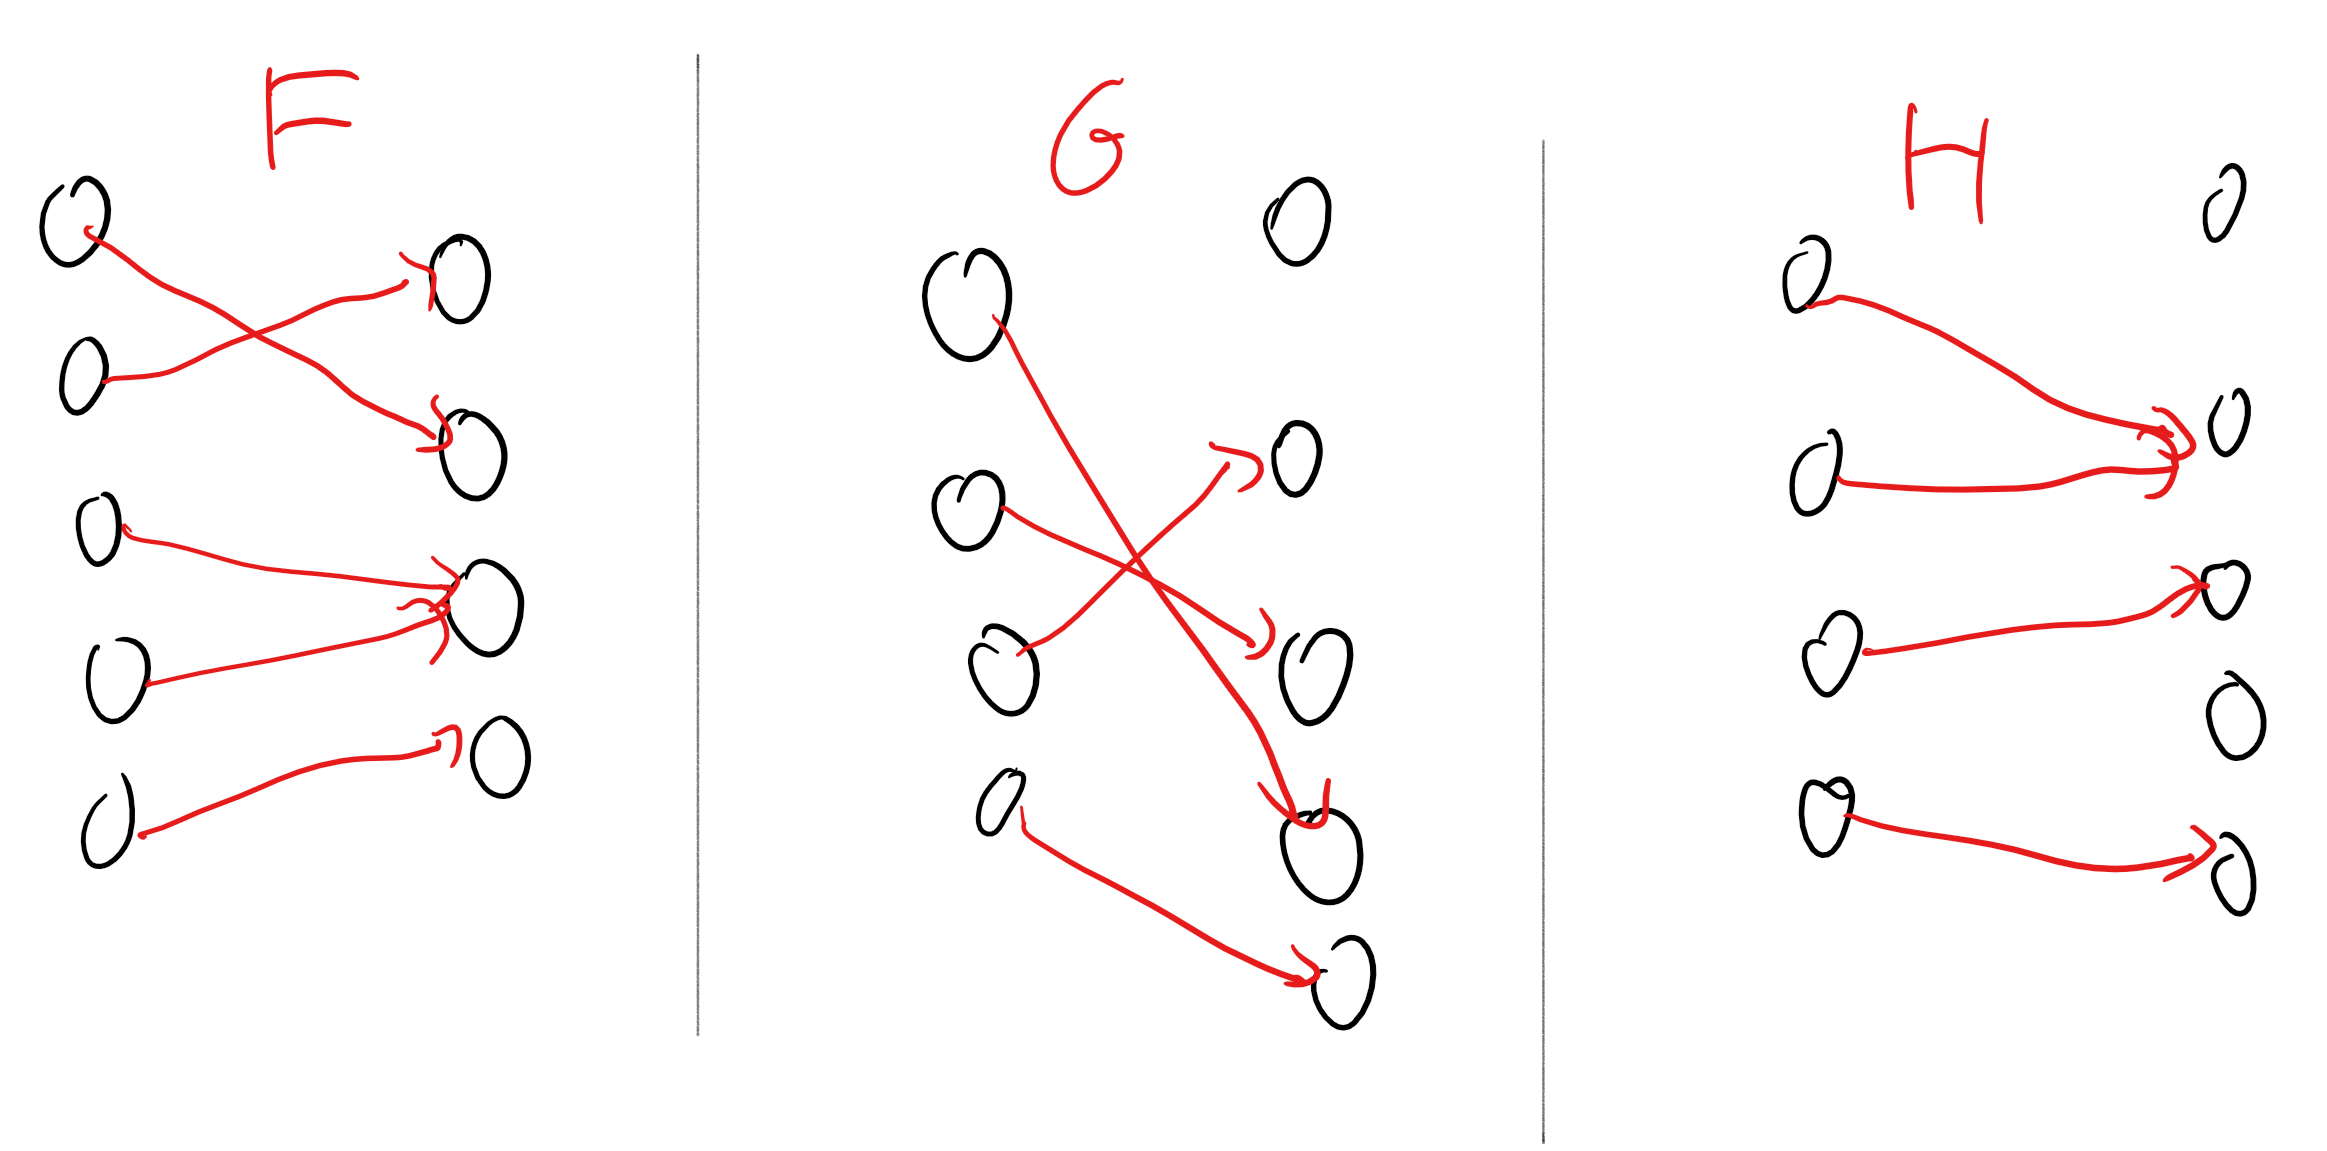
\includegraphics[width=\linewidth, height=1.5in, keepaspectratio]{../figure/functionsdiagram.png}
\caption{We can represent finite functions as a directed graph where we
put an edge from \(x\) to \(f(x)\). The \emph{onto} condition
corresponds to requiring that every vertex in the codomain of the
function has in-degree \emph{at least} one. The \emph{one-to-one}
condition corresponds to requiring that every vertex in the codomain of
the function has in-degree \emph{at most} one. In the examples above
\(F\) is an onto function, \(G\) is one to one, and \(H\) is neither
onto nor one to one.}
\label{functionsdiagrampng}
\end{marginfigure}

\begin{pause} \label[pause]{You-can-find-the-proofs-o}

You can find the proofs of these results in many discrete math texts,
including for example, Section 4.5 in the
\href{https://cs121.boazbarak.org/LLM_data_types.pdf}{Lehman-Leighton-Meyer
notes}. However, I strongly suggest you try to prove them on your own,
or at least convince yourself that they are true by proving special
cases of those for small sizes (e.g., \(|S|=3,|T|=4,|U|=5\)).

\end{pause}

Let us prove one of these facts as an example:

\hypertarget{onetooneimpliesonto}{}
\begin{lemma} \label[lemma]{onetooneimpliesonto}

If \(S,T\) are non-empty sets and \(F:S \rightarrow T\) is one to one,
then there exists an onto function \(G:T \rightarrow S\) such that
\(G(F(s))=s\) for every \(s\in S\).

\end{lemma}

\begin{proof} \label[proof]{Choose-some-s-in-S-We-wil}

Choose some \(s_0 \in S\). We will define the function
\(G:T \rightarrow S\) as follows: for every \(t\in T\), if there is some
\(s\in S\) such that \(F(s)=t\) then set \(G(t)=s\) (the choice of \(s\)
is well defined since by the one-to-one property of \(F\), there cannot
be two distinct \(s,s'\) that both map to \(t\)). Otherwise, set
\(G(t)=s_0\). Now for every \(s\in S\), by the definition of \(G\), if
\(t=F(s)\) then \(G(t)=G(F(s))=s\). Moreover, this also shows that \(G\)
is \emph{onto}, since it means that for every \(s\in S\) there is some
\(t\), namely \(t=F(s)\), such that \(G(t)=s\).

\end{proof}

\subsection{Graphs}\label{graphsec}

\emph{Graphs} are ubiquitous in Computer Science, and many other fields
as well. They are used to model a variety of data types including social
networks, scheduling constraints, road networks, deep neural nets, gene
interactions, correlations between observations, and a great many more.
Formal definitions of several kinds of graphs are given next, but if you
have not seen graphs before in a course, I urge you to read up on them
in one of the sources mentioned in \cref{notesmathchap}.

Graphs come in two basic flavors: \emph{undirected} and
\emph{directed}.\footnote{It is possible, and sometimes useful, to think
  of an undirected graph as the special case of a directed graph that
  has the special property that for every pair \(u,v\) either both the
  edges \((u,v)\) and \((v,u)\) are present or neither of them is.
  However, in many settings there is a significant difference between
  undirected and directed graphs, and so it's typically best to think of
  them as separate categories.}


\begin{marginfigure}[1.5in]
\centering
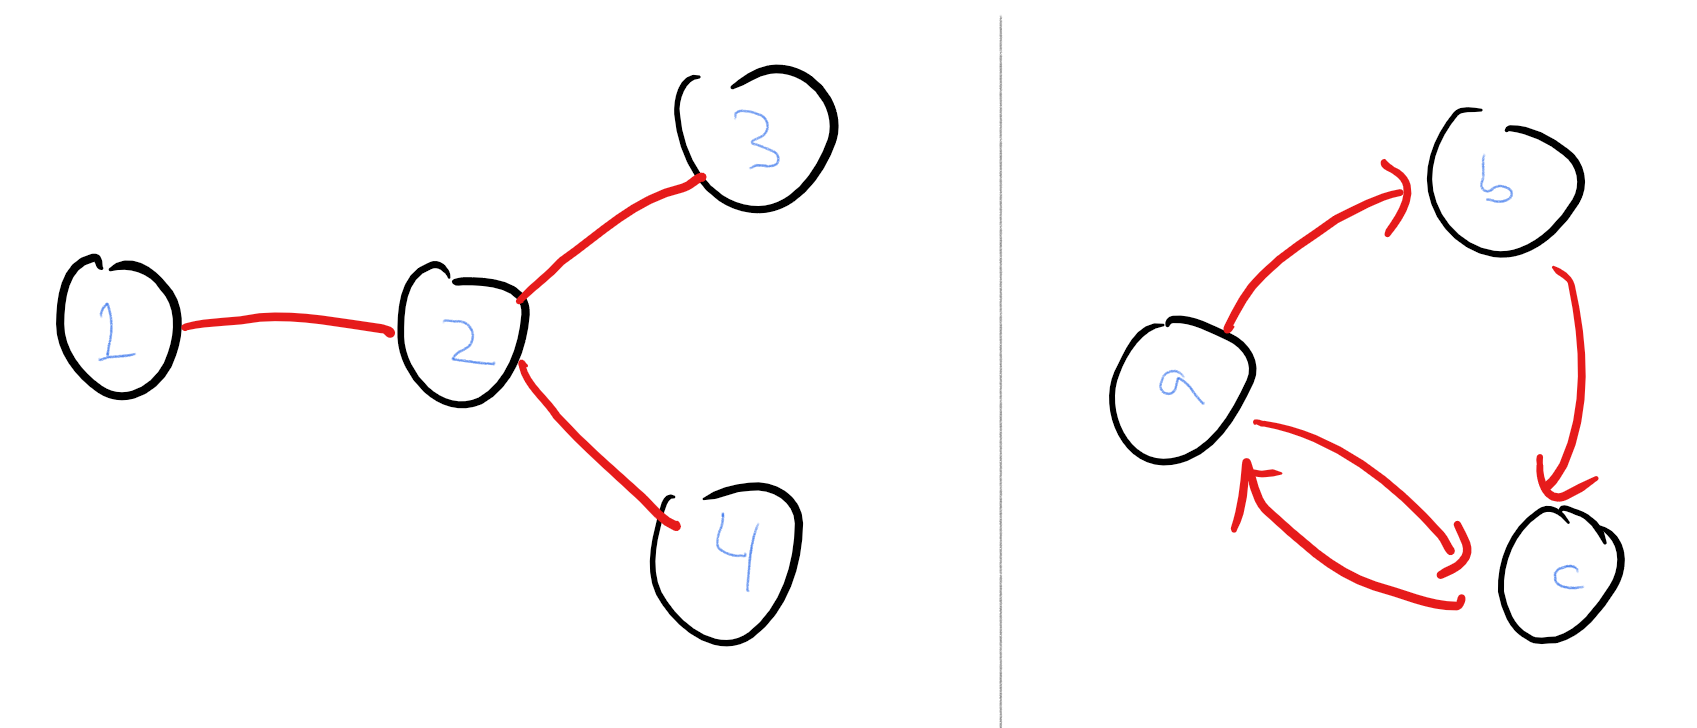
\includegraphics[width=\linewidth, height=1.5in, keepaspectratio]{../figure/graphsexampe.png}
\caption{An example of an undirected and a directed graph. The
undirected graph has vertex set \(\{1,2,3,4\}\) and edge set
\(\{ \{1,2\},\{2,3\},\{2,4\} \}\). The directed graph has vertex set
\(\{a,b,c\}\) and the edge set \(\{ (a,b),(b,c),(c,a),(a,c) \}\).}
\label{graphsexampefig}
\end{marginfigure}

\hypertarget{undirgraph}{}
\begin{definition}[Undirected graphs] \label[definition]{undirgraph}

An \emph{undirected graph} \(G = (V,E)\) consists of a set \(V\) of
\emph{vertices} and a set \(E\) of edges. Every edge is a size two
subset of \(V\). We say that two vertices \(u,v \in V\) are
\emph{neighbors}, if the edge \(\{u,v\}\) is in \(E\).

\end{definition}

Given this definition, we can define several other properties of graphs
and their vertices. We define the \emph{degree} of \(u\) to be the
number of neighbors \(u\) has. A \emph{path} in the graph is a tuple
\((u_0,\ldots,u_k) \in V^{k+1}\), for some \(k>0\) such that \(u_{i+1}\)
is a neighbor of \(u_i\) for every \(i\in [k]\). A \emph{simple path} is
a path \((u_0,\ldots,u_{k-1})\) where all the \(u_i\)'s are distinct. A
\emph{cycle} is a path \((u_0,\ldots,u_k)\) where \(u_0=u_{k}\). We say
that two vertices \(u,v\in V\) are \emph{connected} if either \(u=v\) or
there is a path from \((u_0,\ldots,u_k)\) where \(u_0=u\) and \(u_k=v\).
We say that the graph \(G\) is \emph{connected} if every pair of
vertices in it is connected.

Here are some basic facts about undirected graphs. We give some informal
arguments below, but leave the full proofs as exercises (the proofs can
be found in many of the resources listed in \cref{notesmathchap}).

\hypertarget{degreesegeslem}{}
\begin{lemma} \label[lemma]{degreesegeslem}

In any undirected graph \(G=(V,E)\), the sum of the degrees of all
vertices is equal to twice the number of edges.

\end{lemma}

\cref{degreesegeslem} can be shown by seeing that every edge
\(\{ u,v\}\) contributes twice to the sum of the degrees (once for \(u\)
and the second time for \(v\)).

\hypertarget{conntranslem}{}
\begin{lemma} \label[lemma]{conntranslem}

The connectivity relation is \emph{transitive}, in the sense that if
\(u\) is connected to \(v\), and \(v\) is connected to \(w\), then \(u\)
is connected to \(w\).

\end{lemma}

\cref{conntranslem} can be shown by simply attaching a path of the form
\((u,u_1,u_2,\ldots,u_{k-1},v)\) to a path of the form
\((v,u'_1,\ldots,u'_{k'-1},w)\) to obtain the path
\((u,u_1,\ldots,u_{k-1},v,u'_1,\ldots,u'_{k'-1},w)\) that connects \(u\)
to \(w\).

\hypertarget{simplepathlem}{}
\begin{lemma} \label[lemma]{simplepathlem}

For every undirected graph \(G=(V,E)\) and connected pair \(u,v\), the
shortest path from \(u\) to \(v\) is simple. In particular, for every
connected pair there exists a simple path that connects them.

\end{lemma}

\cref{simplepathlem} can be shown by ``shortcutting'' any non simple
path from \(u\) to \(v\) where the same vertex \(w\) appears twice to
remove it (see \cref{shortcutpathfig}). It is a good exercise to
transforming this intuitive reasoning to a formal proof:


\begin{figure}
\centering
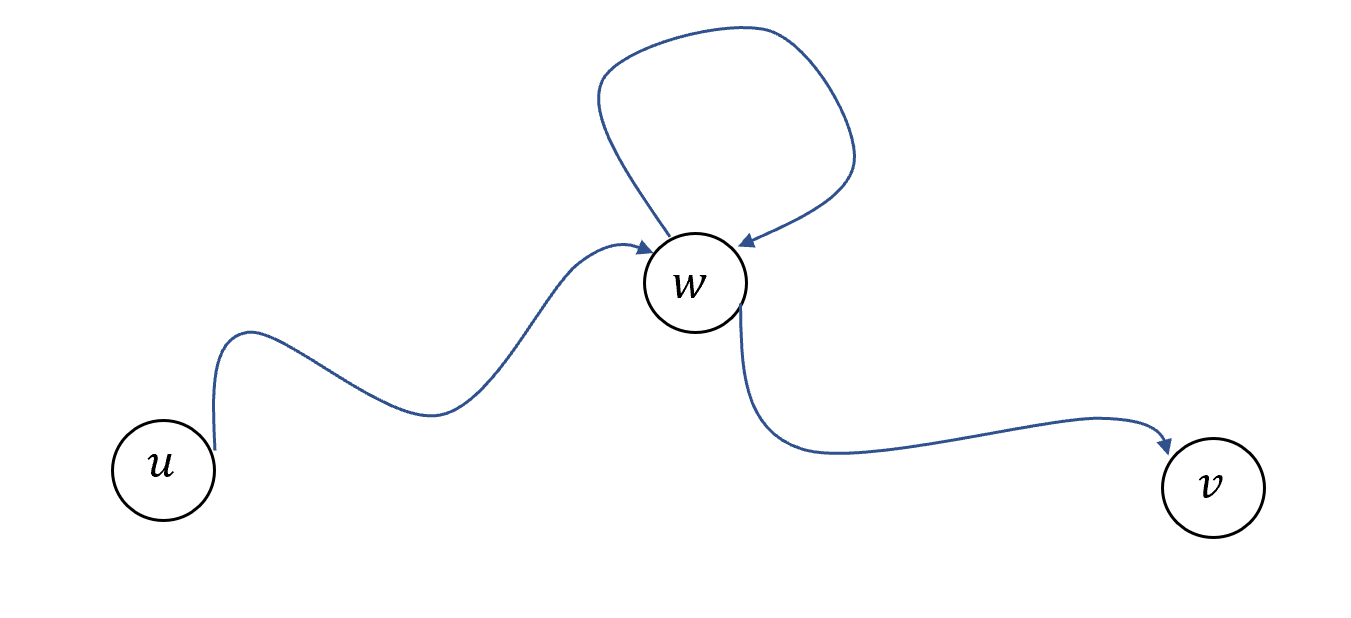
\includegraphics[width=\textwidth, height=0.25\paperheight, keepaspectratio]{../figure/shortcutpath.png}
\caption{If there is a path from \(u\) to \(v\) in a graph that passes
twice through a vertex \(w\) then we can ``shortcut'' it by removing the
loop from \(w\) to itself to find a path from \(u\) to \(v\) that only
passes once through \(w\).}
\label{shortcutpathfig}
\end{figure}

\hypertarget{simplepathlemex}{}
\begin{solvedexercise}[Connected vertices have simple paths] \label[solvedexercise]{simplepathlemex}

Prove \cref{simplepathlem}

\end{solvedexercise}

\begin{solution} \label[solution]{The-proof-follows-the-ide}

The proof follows the idea illustrated in \cref{shortcutpathfig}. One
complication is that there can be more than one vertex that is visited
twice by a path, and so ``shortcutting'' might not necessarily result in
a simple path; we deal with this by looking at a \emph{shortest} path
between \(u\) and \(v\). Details follow.

Let \(G=(V,E)\) be a graph and \(u\) and \(v\) in \(V\) be two connected
vertices in \(G\). We will prove that there is a simple graph between
\(u\) and \(v\). Let \(k\) be the shortest length of a path between
\(u\) and \(v\) and let \(P=(u_0,u_1,u_2,\ldots,u_{k-1},u_k)\) be a
\(k\)-length path from \(u\) to \(v\) (there can be more than one such
path: if so we just choose one of them). (That is \(u_0=u\), \(u_k=v\),
and \((u_\ell,u_{\ell+1})\in E\) for all \(\ell \in [k]\).) We claim
that \(P\) is simple. Indeed, suppose otherwise that there is some
vertex \(w\) that occurs twice in the path: \(w = u_i\) and \(w=u_j\)
for some \(i<j\). Then we can ``shortcut'' the path \(P\) by considering
the path \(P' = (u_0,u_1,\ldots,u_{i-1},w,u_{j+1},\ldots,u_k)\) obtained
by taking the first \(i\) vertices of \(P\) (from \(u_0=0\) to the first
occurrence of \(w\)) and the last \(k-j\) ones (from the vertex
\(u_{j+1}\) following the second occurrence of \(w\) to \(u_k=v\)). The
path \(P'\) is a valid path between \(u\) and \(v\) since every
consecutive pair of vertices in it is connected by an edge (in
particular, since \(w=u_i=w_j\), both \((u_{i-1},w)\) and
\((w,u_{j+1})\) are edges in \(E\)), but since the length of \(P'\) is
\(k-(j-i)<k\), this contradicts the minimality of \(P\).

\end{solution}

\hypertarget{comingupwithproofs}{}
\begin{remark}[Finding proofs] \label[remark]{comingupwithproofs}

\cref{simplepathlemex} is a good example of the process of finding a
proof. You start by ensuring you understand what the statement means,
and then come up with an informal argument why it should be true. You
then transform the informal argument into a rigorous proof. This proof
need not be very long or overly formal, but should clearly establish why
the conclusion of the statement follows from its assumptions.

\end{remark}

The concepts of degrees and connectivity extend naturally to
\emph{directed graphs}, defined as follows.

\hypertarget{directedgraphdef}{}
\begin{definition}[Directed graphs] \label[definition]{directedgraphdef}

A \emph{directed graph} \(G=(V,E)\) consists of a set \(V\) and a set
\(E \subseteq V\times V\) of \emph{ordered pairs} of \(V\). We sometimes
denote the edge \((u,v)\) also as \(u \rightarrow v\). If the edge
\(u \rightarrow v\) is present in the graph then we say that \(v\) is an
\emph{out-neighbor} of \(u\) and \(u\) is an \emph{in-neighbor} of
\(v\).

\end{definition}

A directed graph might contain both \(u \rightarrow v\) and
\(v \rightarrow u\) in which case \(u\) will be both an in-neighbor and
an out-neighbor of \(v\) and vice versa. The \emph{in-degree} of \(u\)
is the number of in-neighbors it has, and the \emph{out-degree} of \(v\)
is the number of out-neighbors it has. A \emph{path} in the graph is a
tuple \((u_0,\ldots,u_k) \in V^{k+1}\), for some \(k>0\) such that
\(u_{i+1}\) is an out-neighbor of \(u_i\) for every \(i\in [k]\). As in
the undirected case, a \emph{simple path} is a path
\((u_0,\ldots,u_{k-1})\) where all the \(u_i\)'s are distinct and a
\emph{cycle} is a path \((u_0,\ldots,u_k)\) where \(u_0=u_{k}\). One
type of directed graphs we often care about is \emph{directed acyclic
graphs} or \emph{DAGs}, which, as their name implies, are directed
graphs without any cycles:

\hypertarget{DAGdef}{}
\begin{definition}[Directed Acyclic Graphs] \label[definition]{DAGdef}

We say that \(G=(V,E)\) is a \emph{directed acyclic graph (DAG)} if it
is a directed graph and there does not exist a list of vertices
\(u_0,u_1,\ldots,u_k \in V\) such that \(u_0=u_k\) and for every
\(i\in [k]\), the edge \(u_i \rightarrow u_{i+1}\) is in \(E\).

\end{definition}

The lemmas we mentioned above have analogs for directed graphs. We again
leave the proofs (which are essentially identical to their undirected
analogs) as exercises.

\hypertarget{diredgreesegeslem}{}
\begin{lemma} \label[lemma]{diredgreesegeslem}

In any directed graph \(G=(V,E)\), the sum of the in-degrees is equal to
the sum of the out-degrees, which is equal to the number of edges.

\end{lemma}

\hypertarget{dirconntranslem}{}
\begin{lemma} \label[lemma]{dirconntranslem}

In any directed graph \(G\), if there is a path from \(u\) to \(v\) and
a path from \(v\) to \(w\), then there is a path from \(u\) to \(w\).

\end{lemma}

\hypertarget{dirsimplepathlem}{}
\begin{lemma} \label[lemma]{dirsimplepathlem}

For every directed graph \(G=(V,E)\) and a pair \(u,v\) such that there
is a path from \(u\) to \(v\), the \emph{shortest path} from \(u\) to
\(v\) is simple.

\end{lemma}

\hypertarget{labeledrem}{}
\begin{remark}[Labeled graphs] \label[remark]{labeledrem}

For some applications we will consider \emph{labeled graphs}, where the
vertices or edges have associated \emph{labels} (which can be numbers,
strings, or members of some other set). We can think of such a graph as
having an associated (possibly partial) \emph{labelling function}
\(L:V \cup E \rightarrow \mathcal{L}\), where \(\mathcal{L}\) is the set
of potential labels. However we will typically not refer explicitly to
this labeling function and simply say things such as ``vertex \(v\) has
the label \(\alpha\)''.

\end{remark}

\subsection{Logic operators and quantifiers}\label{secquantifiers}

If \(P\) and \(Q\) are some statements that can be true or false, then
\(P\) AND \(Q\) (denoted as \(P \wedge Q\)) is a statement that is true
if and only if both \(P\) \emph{and} \(Q\) are true, and \(P\) OR \(Q\)
(denoted as \(P \vee Q\)) is a statement that is true if and only if
either \(P\) \emph{or} \(Q\) is true. The \emph{negation} of \(P\),
denoted as \(\neg P\) or \(\overline{P}\), is true if and only if \(P\)
is false.

Suppose that \(P(x)\) is a statement that depends on some
\emph{parameter} \(x\) (also sometimes known as an \emph{unbound}
variable) in the sense that for every instantiation of \(x\) with a
value from some set \(S\), \(P(x)\) is either true or false. For
example, \(x>7\) is a statement that is not a priori true or false, but
becomes true or false whenever we instantiate \(x\) with some real
number. We denote by \(\forall_{x\in S} P(x)\) the statement that is
true if and only if \(P(x)\) is true \emph{for every}
\(x\in S\).\footnote{In this book, we place the variable bound by a
  quantifier in a subscript and so write \(\forall_{x\in S}P(x)\). Many
  other texts do not use this subscript notation and so will write the
  same statement as \(\forall x\in S, \; P(x)\).} We denote by
\(\exists_{x\in S} P(x)\) the statement that is true if and only if
\emph{there exists} some \(x\in S\) such that \(P(x)\) is true.

For example, the following is a formalization of the true statement that
there exists a natural number \(n\) larger than \(100\) that is not
divisible by \(3\):

\[
\exists_{n\in \N} (n>100) \wedge \left(\forall_{k\in N} k+k+k \neq n\right) \;.
\]

\paragraph{For sufficiently large n.} One expression that we will see
come up time and again in this book is the claim that some statement
\(P(n)\) is true ``for sufficiently large \(n\)''. What this means is
that there exists an integer \(N_0\) such that \(P(n)\) is true for
every \(n>N_0\). We can formalize this as
\(\exists_{N_0\in \N} \forall_{n>N_0} P(n)\).

\subsection{Quantifiers for summations and
products}\label{secquantifierssums}

The following shorthands for summing up or taking products of several
numbers are often convenient. If \(S = \{s_0,\ldots,s_{n-1} \}\) is a
finite set and \(f:S \rightarrow \R\) is a function, then we write
\(\sum_{x\in S} f(x)\) as shorthand for

\[
f(s_0) + f(s_1) + f(s_2) + \ldots + f(s_{n-1}) \;,
\]

and \(\prod_{x\in S} f(x)\) as shorthand for

\[
f(s_0) \cdot f(s_1) \cdot f(s_2) \cdot \ldots \cdot f(s_{n-1}) \;.
\]

For example, the sum of the squares of all numbers from \(1\) to \(100\)
can be written as

\[
\sum_{i\in \{1,\ldots,100\}} i^2 \;. \label{eqsumsquarehundred}
\]

Since summing up over intervals of integers is so common, there is a
special notation for it. For every two integers, \(a \leq b\),
\(\sum_{i=a}^b f(i)\) denotes \(\sum_{i\in S} f(i)\) where
\(S =\{ x\in \Z : a \leq x \leq b \}\). Hence, we can write the sum
\eqref{eqsumsquarehundred} as

\[
\sum_{i=1}^{100} i^2 \;.
\]

\subsection{Parsing formulas: bound and free
variables}\label{boundvarsec}

In mathematics, as in coding, we often have symbolic ``variables'' or
``parameters''. It is important to be able to understand, given some
formula, whether a given variable is \emph{bound} or \emph{free} in this
formula. For example, in the following statement \(n\) is free but \(a\)
and \(b\) are bound by the \(\exists\) quantifier:

\[
\exists_{a,b \in \N} (a \neq 1) \wedge (a \neq n) \wedge (n = a \times b) \label{aboutnstmt}
\]

Since \(n\) is free, it can be set to any value, and the truth of the
statement \eqref{aboutnstmt} depends on the value of \(n\). For example,
if \(n=8\) then \eqref{aboutnstmt} is true, but for \(n=11\) it is
false. (Can you see why?)

The same issue appears when parsing code. For example, in the following
snippet from the C programming language

\begin{code}
for (int i=0 ; i<n ; i=i+1) {
    printf("*");
}
\end{code}

the variable \texttt{i} is bound within the \texttt{for} block but the
variable \texttt{n} is free.

The main property of bound variables is that we can \emph{rename} them
(as long as the new name doesn't conflict with another used variable)
without changing the meaning of the statement. Thus for example the
statement

\[
\exists_{x,y \in \N} (x \neq 1) \wedge (x \neq n) \wedge (n = x \times y) \label{aboutnstmttwo}
\]

is \emph{equivalent} to \eqref{aboutnstmt} in the sense that it is true
for exactly the same set of \(n\)'s.

Similarly, the code

\begin{code}
for (int j=0 ; j<n ; j=j+1) {
    printf("*");
}
\end{code}

produces the same result as the code above that used \texttt{i} instead
of \texttt{j}.

\hypertarget{notationrem}{}
\begin{remark}[Aside: mathematical vs programming notation] \label[remark]{notationrem}

Mathematical notation has a lot of similarities with programming
language, and for the same reasons. Both are formalisms meant to convey
complex concepts in a precise way. However, there are some cultural
differences. In programming languages, we often try to use meaningful
variable names such as \texttt{NumberOfVertices} while in math we often
use short identifiers such as \(n\). Part of it might have to do with
the tradition of mathematical proofs as being handwritten and verbally
presented, as opposed to typed up and compiled. Another reason is if the
wrong variable name is used in a proof, at worst is causes confusion to
readers; when the wrong variable name is used in a program, planes might
crash, patients might die, and rockets could explode.

One consequence of that is that in mathematics we often end up reusing
identifiers, and also ``run out'' of letters and hence use Greek letters
too, as well as distinguish between small and capital letters and
different font faces. Similarly, mathematical notation tends to use
quite a lot of ``overloading'', using operators such as \(+\) for a
great variety of objects (e.g., real numbers, matrices, finite field
elements, etc..), and assuming that the meaning can be inferred from the
context.

Both fields have a notion of ``types'', and in math we often try to
reserve certain letters for variables of a particular type. For example,
variables such as \(i,j,k,\ell,m,n\) will often denote integers, and
\(\epsilon\) will often denote a small positive real number (see
\cref{notationsec} for more on these conventions). When reading or
writing mathematical texts, we usually don't have the advantage of a
``compiler'' that will check type safety for us. Hence it is important
to keep track of the type of each variable, and see that the operations
that are performed on it ``make sense''.

Kun's book \cite{Kun18} contains an extensive discussion on the
similarities and differences between the cultures of mathematics and
programming.

\end{remark}

\subsection{Asymptotics and Big-\(O\) notation}\label{secbigohnotation}

\begin{quote}
\emph{``\(\log\log\log n\) has been proved to go to infinity, but has
never been observed to do so.''}, Anonymous, quoted by Carl Pomerance
(2000)
\end{quote}

It is often very cumbersome to describe precisely quantities such as
running time and is also not needed, since we are typically mostly
interested in the ``higher order terms''. That is, we want to understand
the \emph{scaling behavior} of the quantity as the input variable grows.
For example, as far as running time goes, the difference between an
\(n^5\)-time algorithm and an \(n^2\)-time one is much more significant
than the difference between an \(100n^2 + 10n\) time algorithm and an
\(10n^2\) time algorithm. For this purpose, \(O\)-notation is extremely
useful as a way to ``declutter'' our text and focus our attention on
what really matters. For example, using \(O\)-notation, we can say that
both \(100n^2 + 10n\) and \(10n^2\) are simply \(\Theta(n^2)\) (which
informally means ``the same up to constant factors''), while
\(n^2 = o(n^5)\) (which informally means that \(n^2\) is ``much smaller
than'' \(n^5\)).

Generally (though still informally), if \(F,G\) are two functions
mapping natural numbers to non-negative reals, then ``\(F=O(G)\)'' means
that \(F(n) \leq G(n)\) if we don't care about constant factors, while
``\(F=o(G)\)'' means that \(F\) is much smaller than \(G\), in the sense
that no matter by what constant factor we multiply \(F\), if we take
\(n\) to be large enough then \(G\) will be bigger (for this reason,
sometimes \(F=o(G)\) is written as \(F \ll G\)). We will write
\(F= \Theta(G)\) if \(F=O(G)\) and \(G=O(F)\), which one can think of as
saying that \(F\) is the same as \(G\) if we don't care about constant
factors. More formally, we define Big-\(O\) notation as follows:

\hypertarget{bigohdef}{}
\begin{definition}[Big-$O$ notation] \label[definition]{bigohdef}

Let \(\R_+= \{ x\in \R \;|\; x>0\}\) be the set of positive real
numbers. For two functions \(F,G: \N \rightarrow \R_+\), we say that
\emph{\(F=O(G)\)} if there exist numbers \(a,N_0 \in \N\) such that
\(F(n) \leq a\cdot G(n)\) for every \(n>N_0\). We say that
\(F= \Theta(G)\) if \(F=O(G)\) and \(G=O(F)\). We say that
\(F=\Omega(G)\) if \(G=O(F)\).

We say that \emph{\(F =o(G)\)} if for every \(\epsilon>0\) there is some
\(N_0\) such that \(F(n) <\epsilon G(n)\) for every \(n>N_0\). We say
that \(F =\omega(G)\) if \(G=o(F)\).

\end{definition}


\begin{marginfigure}
\centering
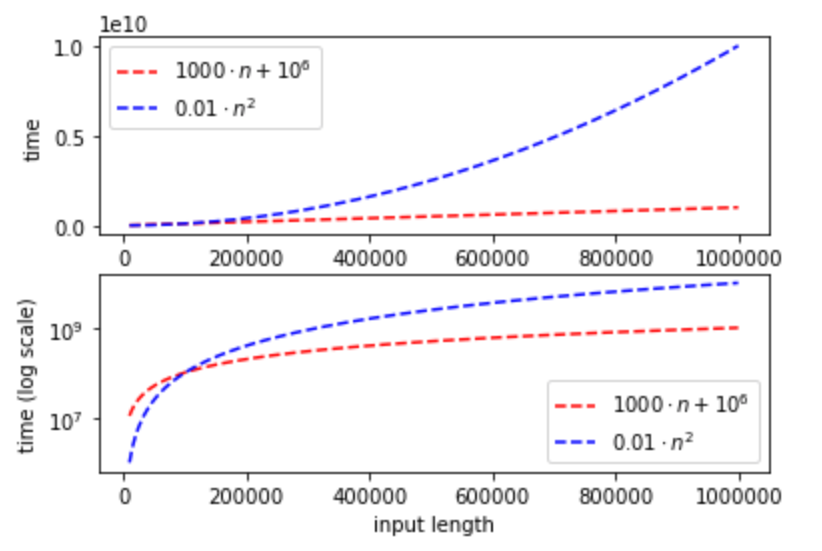
\includegraphics[width=\linewidth, height=1.5in, keepaspectratio]{../figure/nvsnsquared.png}
\caption{If \(F(n)=o(G(n))\) then for sufficiently large \(n\), \(F(n)\)
will be smaller than \(G(n)\). For example, if Algorithm \(A\) runs in
time \(1000\cdot n+10^6\) and Algorithm \(B\) runs in time
\(0.01\cdot n^2\) then even though \(B\) might be more efficient for
smaller inputs, when the inputs get sufficiently large, \(A\) will run
\emph{much} faster than \(B\).}
\label{nvsnsquaredfig}
\end{marginfigure}

It's often convenient to use ``anonymous functions'' in the context of
\(O\)-notation. For example, when we write a statement such as
\(F(n) = O(n^3)\), we mean that \(F=O(G)\) where \(G\) is the function
defined by \(G(n)=n^3\). Chapter 7 in
\href{http://www.cs.yale.edu/homes/aspnes/classes/202/notes.pdf}{Jim
Apsnes' notes on discrete math} provides a good summary of \(O\)
notation; see also \href{http://discrete.gr/complexity/}{this tutorial}
for a gentler and more programmer-oriented introduction.

\emph{\(O\) is not equality.} Using the equality sign for \(O\)-notation
is extremely common, but is somewhat of a misnomer, since a statement
such as \(F = O(G)\) really means that \(F\) is in the set
\(\{ G' : \exists_{N,c} \text{ s.t. } \forall_{n>N} G'(n) \leq c G(n) \}\).
If anything, it makes more sense to use \emph{inequalities} and write
\(F \leq O(G)\) and \(F \geq \Omega(G)\), reserving equality for
\(F = \Theta(G)\), and so we will sometimes use this notation too, but
since the equality notation is quite firmly entrenched we often stick to
it as well. (Some texts write \(F \in O(G)\) instead of \(F = O(G)\),
but we will not use this notation.) Despite the misleading equality
sign, you should remember that a statement such as \(F = O(G)\) means
that \(F\) is ``at most'' \(G\) in some rough sense when we ignore
constants, and a statement such as \(F = \Omega(G)\) means that \(F\) is
``at least'' \(G\) in the same rough sense.

\subsection{Some ``rules of thumb'' for Big-\(O\)
notation}\label{Some-rules-of-thumb-for-B}

There are some simple heuristics that can help when trying to compare
two functions \(F\) and \(G\):

\begin{itemize}
\item
  Multiplicative constants don't matter in \(O\)-notation, and so if
  \(F(n)=O(G(n))\) then \(100F(n)=O(G(n))\).
\item
  When adding two functions, we only care about the larger one. For
  example, for the purpose of \(O\)-notation, \(n^3+100n^2\) is the same
  as \(n^3\), and in general in any polynomial, we only care about the
  larger exponent.
\item
  For every two constants \(a,b>0\), \(n^a = O(n^b)\) if and only if
  \(a \leq b\), and \(n^a = o(n^b)\) if and only if \(a<b\). For
  example, combining the two observations above,
  \(100n^2 + 10n + 100 = o(n^3)\).
\item
  Polynomial is always smaller than exponential:
  \(n^a = o(2^{n^\epsilon})\) for every two constants \(a>0\) and
  \(\epsilon>0\) even if \(\epsilon\) is much smaller than \(a\). For
  example, \(100n^{100} = o(2^{\sqrt{n}})\).
\item
  Similarly, logarithmic is always smaller than polynomial:
  \((\log n)^a\) (which we write as \(\log^a n\)) is \(o(n^\epsilon)\)
  for every two constants \(a,\epsilon>0\). For example, combining the
  observations above, \(100n^2 \log^{100} n = o(n^3)\).
\end{itemize}

\hypertarget{bigonotime}{}
\begin{remark}[Big $O$ for other applications (optional)] \label[remark]{bigonotime}

While Big-\(O\) notation is often used to analyze running time of
algorithms, this is by no means the only application. We can use \(O\)
notation to bound asymptotic relations between any functions mapping
integers to positive numbers. It can be used regardless of whether these
functions are a measure of running time, memory usage, or any other
quantity that may have nothing to do with computation. Here is one
example which is unrelated to this book (and hence one that you can feel
free to skip): one way to state the
\href{https://en.wikipedia.org/wiki/Riemann_hypothesis}{Riemann
Hypothesis} (one of the most famous open questions in mathematics) is
that it corresponds to the conjecture that the number of primes between
\(0\) and \(n\) is equal to \(\int_2^n \tfrac{1}{\ln x} dx\) up to an
additive error of magnitude at most \(O(\sqrt{n}\log n)\).

\end{remark}

\section{Proofs}\label{proofsbackgroundsec}

Many people think of mathematical proofs as a sequence of logical
deductions that starts from some axioms and ultimately arrives at a
conclusion. In fact, some dictionaries
\href{http://www.thefreedictionary.com/mathematical+proof}{define}
proofs that way. This is not entirely wrong, but at its essence
mathematical proof of a statement X is simply an argument that convinces
the reader that X is true beyond a shadow of a doubt.

To produce such a proof you need to:

\begin{enumerate}
\def\labelenumi{\arabic{enumi}.}
\item
  Understand precisely what X means.
\item
  Convince \emph{yourself} that X is true.
\item
  Write your reasoning down in plain, precise and concise English (using
  formulas or notation only when they help clarity).
\end{enumerate}

In many cases, the first part is the most important one. Understanding
what a statement means is oftentimes more than halfway towards
understanding why it is true. In third part, to convince the reader
beyond a shadow of a doubt, we will often want to break down the
reasoning to ``basic steps'', where each basic step is simple enough to
be ``self evident''. The combination of all steps yields the desired
statement.

\subsection{Proofs and programs}\label{Proofs-and-programs}

There is a great deal of similarity between the process of writing
\emph{proofs} and that of writing \emph{programs}, and both require a
similar set of skills. Writing a \emph{program} involves:

\begin{enumerate}
\def\labelenumi{\arabic{enumi}.}
\item
  Understanding what is the \emph{task} we want the program to achieve.
\item
  Convincing \emph{yourself} that the task can be achieved by a
  computer, perhaps by planning on a whiteboard or notepad how you will
  break it up to simpler tasks.
\item
  Converting this plan into code that a compiler or interpreter can
  understand, by breaking up each task into a sequence of the basic
  operations of some programming language.
\end{enumerate}

In programs as in proofs, step 1 is often the most important one. A key
difference is that the reader for proofs is a human being and the reader
for programs is a computer. (This difference is eroding with time as
more proofs are being written in a \emph{machine verifiable} form;
moreover, to ensure correctness and maintainability of programs, it is
important that they can be read and understood by humans.) Thus our
emphasis is on \emph{readability} and having a \emph{clear logical flow}
for our proof (which is not a bad idea for programs as well). When
writing a proof, you should think of your audience as an intelligent but
highly skeptical and somewhat petty reader, that will ``call foul'' at
every step that is not well justified.

\subsection{Proof writing style}\label{Proof-writing-style}

A mathematical proof is a piece of writing, but it is a specific genre
of writing with certain conventions and preferred styles. As in any
writing, practice makes perfect, and it is also important to revise your
drafts for clarity.

In a proof for the statement \(X\), all the text between the words
\textbf{``Proof:''} and \textbf{``QED''} should be focused on
establishing that \(X\) is true. Digressions, examples, or ruminations
should be kept outside these two words, so they do not confuse the
reader. The proof should have a clear logical flow in the sense that
every sentence or equation in it should have some purpose and it should
be crystal-clear to the reader what this purpose is. When you write a
proof, for every equation or sentence you include, ask yourself:

\begin{enumerate}
\def\labelenumi{\arabic{enumi}.}
\item
  Is this sentence or equation stating that some statement is true?
\item
  If so, does this statement follow from the previous steps, or are we
  going to establish it in the next step?
\item
  What is the \emph{role} of this sentence or equation? Is it one step
  towards proving the original statement, or is it a step towards
  proving some intermediate claim that you have stated before?
\item
  Finally, would the answers to questions 1-3 be clear to the reader? If
  not, then you should reorder, rephrase or add explanations.
\end{enumerate}

Some helpful resources on mathematical writing include
\href{https://sites.math.washington.edu/~lee/Writing/writing-proofs.pdf}{this
handout by Lee},
\href{https://math.berkeley.edu/~hutching/teach/proofs.pdf}{this handout
by Hutching}, as well as several of the excellent handouts in
\href{http://web.stanford.edu/class/cs103/}{Stanford's CS 103 class}.

\subsection{Patterns in proofs}\label{Patterns-in-proofs}

\begin{quote}
\emph{``If it was so, it might be; and if it were so, it would be; but
as it isn't, it ain't. That's logic.''}, Lewis Carroll, \emph{Through
the looking-glass}.
\end{quote}

Just like in programming, there are several common patterns of proofs
that occur time and again. Here are some examples:

\paragraph{Proofs by contradiction:} One way to prove that \(X\) is true
is to show that if \(X\) was false it would result in a contradiction.
Such proofs often start with a sentence such as ``Suppose, towards a
contradiction, that \(X\) is false'' and end with deriving some
contradiction (such as a violation of one of the assumptions in the
theorem statement). Here is an example:

\begin{lemma} \label[lemma]{There-are-no-natural-numb}

There are no natural numbers \(a,b\) such that
\(\sqrt{2} = \tfrac{a}{b}\).

\end{lemma}

\begin{proof} \label[proof]{Suppose-towards-a-contrad}

Suppose, towards a contradiction that this is false, and so let
\(a\in \N\) be the smallest number such that there exists some
\(b\in\N\) satisfying \(\sqrt{2}=\tfrac{a}{b}\). Squaring this equation
we get that \(2=a^2/b^2\) or \(a^2=2b^2\) \((*)\). But this means that
\(a^2\) is \emph{even}, and since the product of two odd numbers is odd,
it means that \(a\) is even as well, or in other words, \(a = 2a'\) for
some \(a' \in \N\). Yet plugging this into \((*)\) shows that
\(4a'^2 = 2b^2\) which means \(b^2 = 2a'^2\) is an even number as well.
By the same considerations as above we get that \(b\) is even and hence
\(a/2\) and \(b/2\) are two natural numbers satisfying
\(\tfrac{a/2}{b/2}=\sqrt{2}\), contradicting the minimality of \(a\).

\end{proof}

\paragraph{Proofs of a universal statement:} Often we want to prove a
statement \(X\) of the form ``Every object of type \(O\) has property
\(P\).'' Such proofs often start with a sentence such as ``Let \(o\) be
an object of type \(O\)'' and end by showing that \(o\) has the property
\(P\). Here is a simple example:

\begin{lemma} \label[lemma]{For-every-natural-number-}

For every natural number \(n\in N\), either \(n\) or \(n+1\) is even.

\end{lemma}

\begin{proof} \label[proof]{Let-nin-N-be-some-number-}

Let \(n\in N\) be some number. If \(n/2\) is a whole number then we are
done, since then \(n=2(n/2)\) and hence it is even. Otherwise,
\(n/2+1/2\) is a whole number, and hence \(2(n/2+1/2)=n+1\) is even.

\end{proof}

\paragraph{Proofs of an implication:} Another common case is that the
statement \(X\) has the form ``\(A\) implies \(B\)''. Such proofs often
start with a sentence such as ``Assume that \(A\) is true'' and end with
a derivation of \(B\) from \(A\). Here is a simple example:

\begin{lemma} \label[lemma]{If-b-geq-ac-then-there-is}

If \(b^2 \geq 4ac\) then there is a solution to the quadratic equation
\(ax^2 + bx + c =0\).

\end{lemma}

\begin{proof} \label[proof]{Suppose-that-b-geq-ac-The}

Suppose that \(b^2 \geq 4ac\). Then \(d = b^2 - 4ac\) is a non-negative
number and hence it has a square root \(s\). Thus \(x = (-b+s)/(2a)\)
satisfies \[
\begin{aligned}
ax^2 + bx + c &= a(-b+s)^2/(4a^2) + b(-b+s)/(2a) + c \\
&= (b^2-2bs+s^2)/(4a)+(-b^2+bs)/(2a)+c \;. \label{eq:quadeq}
\end{aligned}
\]

\end{proof}

Rearranging the terms of \eqref{eq:quadeq} we get \[
s^2/(4a)+c- b^2/(4a) = (b^2-4ac)/(4a) + c - b^2/(4a) = 0
\]

\paragraph{Proofs of equivalence:} If a statement has the form ``\(A\)
if and only if \(B\)'' (often shortened as ``\(A\) iff \(B\)'') then we
need to prove both that \(A\) implies \(B\) and that \(B\) implies
\(A\). We call the implication that \(A\) implies \(B\) the ``only if''
direction, and the implication that \(B\) implies \(A\) the ``if''
direction.

\paragraph{Proofs by combining intermediate claims:} When a proof is
more complex, it is often helpful to break it apart into several steps.
That is, to prove the statement \(X\), we might first prove statements
\(X_1\),\(X_2\), and \(X_3\) and then prove that
\(X_1 \wedge X_2 \wedge X_3\) implies \(X\). (Recall that \(\wedge\)
denotes the logical AND operator.)

\paragraph{Proofs by case distinction:} This is a special case of the
above, where to prove a statement \(X\) we split into several cases
\(C_1,\ldots,C_k\), and prove that \textbf{(a)} the cases are
\emph{exhaustive}, in the sense that \emph{one} of the cases \(C_i\)
must happen and \textbf{(b)} go one by one and prove that each one of
the cases \(C_i\) implies the result \(X\) that we are after.

\paragraph{Proofs by induction:} We discuss induction and give an
example in \cref{inductionsec} below. We can think of such proofs as a
variant of the above, where we have an unbounded number of intermediate
claims \(X_0,X_2,\ldots,X_k\), and we prove that \(X_0\) is true, as
well as that \(X_0\) implies \(X_1\), and that \(X_0 \wedge X_1\)
implies \(X_2\), and so on and so forth. The website for CMU course
15-251 contains a
\href{http://www.cs.cmu.edu/~./15251/notes/induction-pitfalls.pdf}{useful
handout} on potential pitfalls when making proofs by induction.

\paragraph{Without loss of generality (w.l.o.g):} This term can be
initially quite confusing. It is essentially a way to simplify proofs by
case distinctions. The idea is that if Case 1 is equal to Case 2 up to a
change of variables or a similar transformation, then the proof of Case
1 will also imply the proof of Case 2. It is always a statement that
should be viewed with suspicion. Whenever you see it in a proof, ask
yourself if you understand \emph{why} the assumption made is truly
without loss of generality, and when you use it, try to see if the use
is indeed justified. When writing a proof, sometimes it might be easiest
to simply repeat the proof of the second case (adding a remark that the
proof is very similar to the first one).

\hypertarget{lamportrem}{}
\begin{remark}[Hierarchical Proofs (optional)] \label[remark]{lamportrem}

Mathematical proofs are ultimately written in English prose. The
well-known computer scientist
\href{https://en.wikipedia.org/wiki/Leslie_Lamport}{Leslie Lamport}
argues that this is a problem, and proofs should be written in a more
formal and rigorous way. In his
\href{https://lamport.azurewebsites.net/pubs/proof.pdf}{manuscript} he
proposes an approach for \emph{structured hierarchical proofs}, that
have the following form:

\begin{itemize}
\item
  A proof for a statement of the form ``If \(A\) then \(B\)'' is a
  sequence of numbered claims, starting with the assumption that \(A\)
  is true, and ending with the claim that \(B\) is true.
\item
  Every claim is followed by a proof showing how it is derived from the
  previous assumptions or claims.
\item
  The proof for each claim is itself a sequence of subclaims.
\end{itemize}

The advantage of Lamport's format is that the role that every sentence
in the proof plays is very clear. It is also much easier to transform
such proofs into machine-checkable forms. The disadvantage is that such
proofs can be tedious to read and write, with less differentiation
between the important parts of the arguments versus the more routine
ones.

\end{remark}

\section{Extended example: Topological Sorting}\label{topsortsec}

In this section we will prove the following: every directed acyclic
graph (DAG, see \cref{DAGdef}) can be arranged in layers so that for all
directed edges \(u \rightarrow v\), the layer of \(v\) is larger than
the layer of \(u\). This result is known as
\href{https://goo.gl/QUskBc}{topological sorting} and is used in many
applications, including task scheduling, build systems, software package
management, spreadsheet cell calculations, and many others (see
\cref{topologicalsortfig}). In fact, we will also use it ourselves later
on in this book.


\begin{figure}
\centering
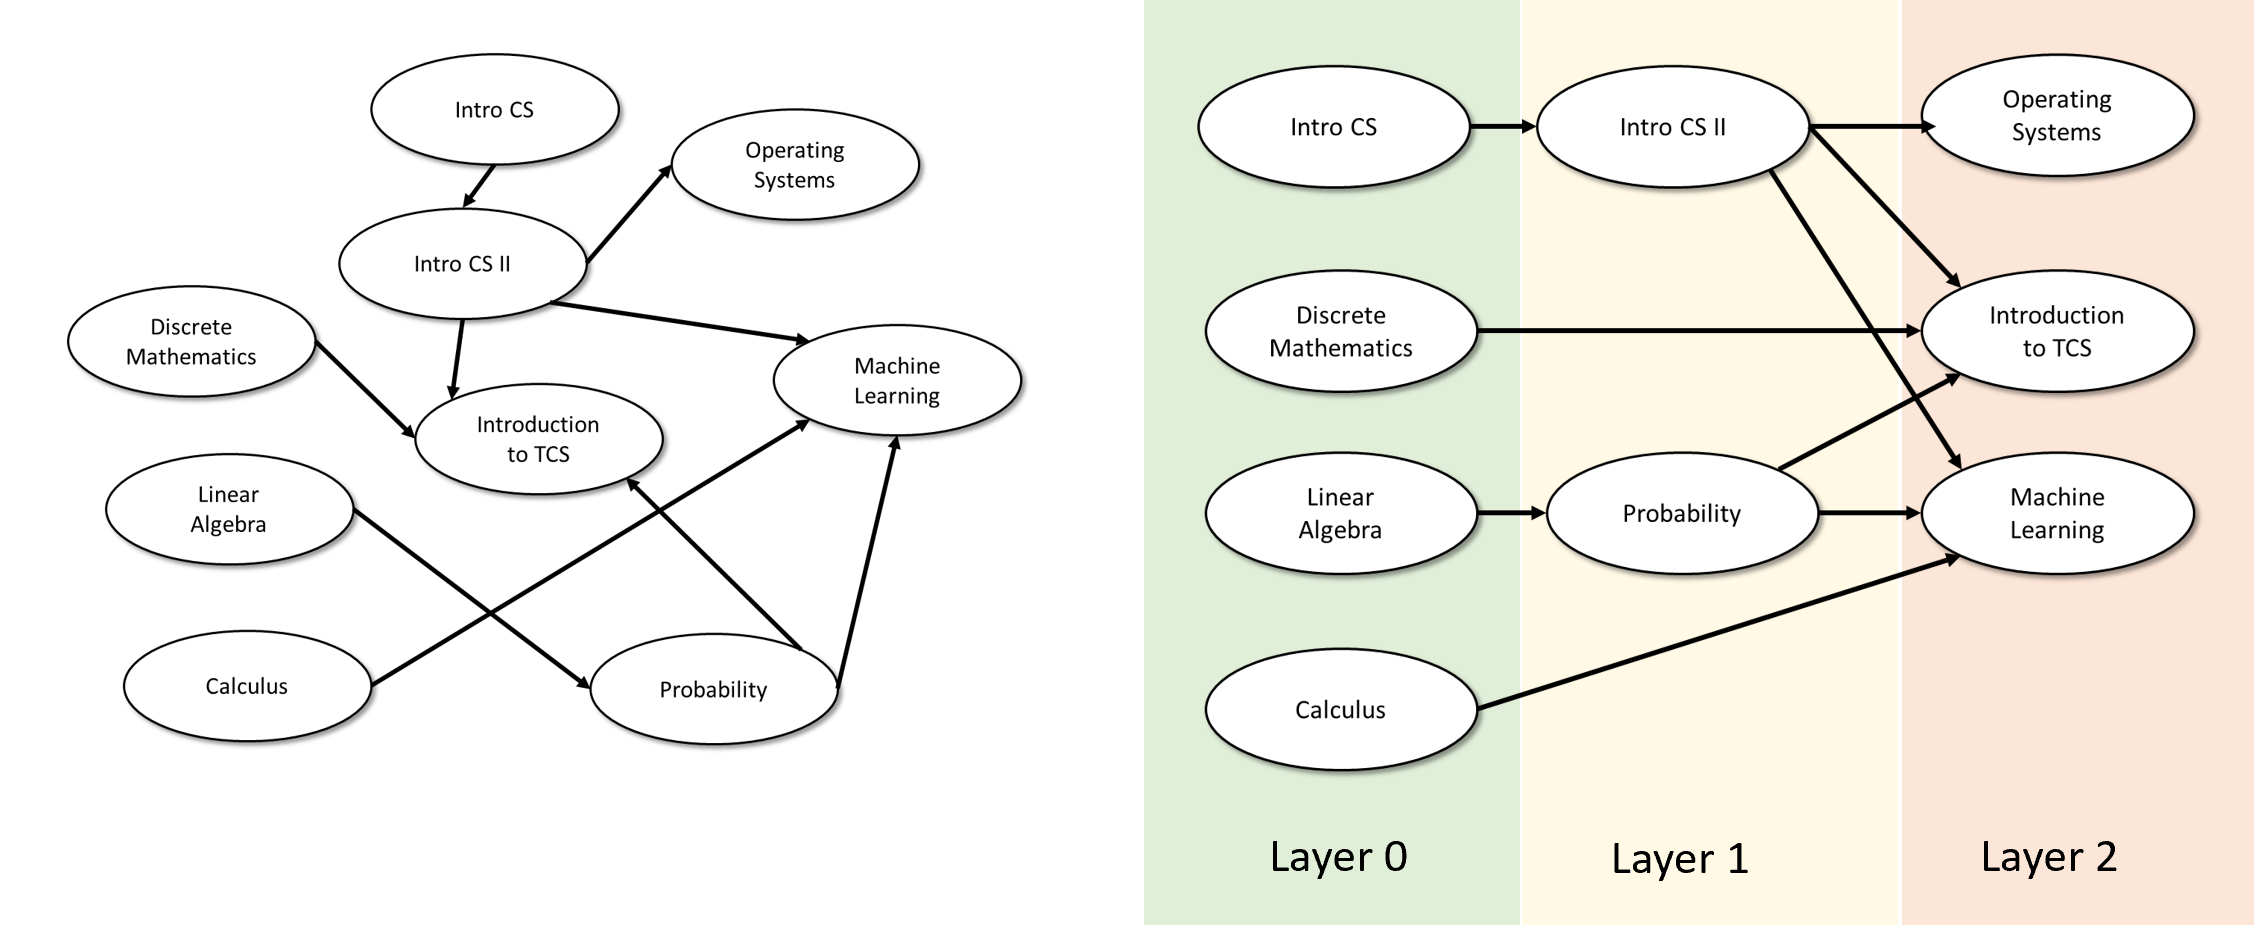
\includegraphics[width=\textwidth, height=0.25\paperheight, keepaspectratio]{../figure/topologicalsort.png}
\caption{An example of \emph{topological sorting}. We consider a
directed graph corresponding to a prerequisite graph of the courses in
some Computer Science program. The edge \(u \rightarrow v\) means that
the course \(u\) is a prerequisite for the course \(v\). A
\emph{layering} or ``topological sorting'' of this graph is the same as
mapping the courses to semesters so that if we decide to take the course
\(v\) in semester \(f(v)\), then we have already taken all the
prerequisites for \(v\) (i.e., its in-neighbors) in prior semesters.}
\label{topologicalsortfig}
\end{figure}

We start with the following definition. A \emph{layering} of a directed
graph is a way to assign for every vertex \(v\) a natural number
(corresponding to its layer), such that \(v\)'s in-neighbors are in
lower-numbered layers than \(v\), and \(v\)'s out-neighbors are in
higher-numbered layers. The formal definition is as follows:

\hypertarget{layeringdef}{}
\begin{definition}[Layering of a DAG] \label[definition]{layeringdef}

Let \(G=(V,E)\) be a directed graph. A \emph{layering} of \(G\) is a
function \(f:V \rightarrow \N\) such that for every edge
\(u \rightarrow v\) of \(G\), \(f(u) < f(v)\).

\end{definition}

In this section we prove that a directed graph is acyclic if and only if
it has a valid layering.

\hypertarget{topologicalsortthm}{}
\begin{theorem}[Topological Sort] \label[theorem]{topologicalsortthm}

Let \(G\) be a directed graph. Then \(G\) is acyclic if and only if
there exists a layering \(f\) of \(G\).

\end{theorem}

To prove such a theorem, we need to first understand what it means.
Since it is an ``if and only if'' statement, \cref{topologicalsortthm}
corresponds to two statements:

\hypertarget{acyclictosortlem}{}
\begin{lemma} \label[lemma]{acyclictosortlem}

For every directed graph \(G\), if \(G\) is acyclic then it has a
layering.

\end{lemma}

\hypertarget{sorttoacycliclem}{}
\begin{lemma} \label[lemma]{sorttoacycliclem}

For every directed graph \(G\), if \(G\) has a layering, then it is
acyclic.

\end{lemma}

To prove \cref{topologicalsortthm} we need to prove both
\cref{acyclictosortlem} and \cref{sorttoacycliclem}.
\cref{sorttoacycliclem} is actually not that hard to prove. Intuitively,
if \(G\) contains a \emph{cycle}, then it cannot be the case that all
edges on the cycle increase in layer number, since if we travel along
the cycle at some point we must come back to the place we started from.
The formal proof is as follows:

\begin{proof} \label[proof]{Let-GVE-be-a-directed-gra}

Let \(G=(V,E)\) be a directed graph and let \(f:V \rightarrow \N\) be a
layering of \(G\) as per \cref{layeringdef} . Suppose, towards a
contradiction, that \(G\) is not acyclic, and hence there exists some
cycle \(u_0,u_1,\ldots,u_k\) such that \(u_0=u_k\) and for every
\(i\in [k]\) the edge \(u_i \rightarrow u_{i+1}\) is present in \(G\).
Since \(f\) is a layering, for every \(i \in [k]\),
\(f(u_i) < f(u_{i+1})\), which means that \[
f(u_0) < f(u_1)  < \cdots  < f(u_k)
\] but this is a contradiction since \(u_0=u_k\) and hence
\(f(u_0)=f(u_k)\).

\end{proof}

\cref{acyclictosortlem} corresponds to the more difficult (and useful)
direction. To prove it, we need to show how given an arbitrary DAG
\(G\), we can come up with a layering of the vertices of \(G\) so that
all edges ``go up''.

\begin{pause} \label[pause]{If-you-have-not-seen-the-}

If you have not seen the proof of this theorem before (or don't remember
it), this would be an excellent point to pause and try to prove it
yourself. One way to do it would be to describe an \emph{algorithm} that
given as input a directed acyclic graph \(G\) on \(n\) vertices and
\(n-2\) or fewer edges, constructs an array \(F\) of length \(n\) such
that for every edge \(u \rightarrow v\) in the graph \(F[u] < F[v]\).

\end{pause}

\subsection{Mathematical induction}\label{inductionsec}

There are several ways to prove \cref{acyclictosortlem}. One approach to
do is to start by proving it for small graphs, such as graphs with 1, 2
or 3 vertices (see \cref{topsortexamplesfig}, for which we can check all
the cases, and then try to extend the proof for larger graphs. The
technical term for this proof approach is \emph{proof by induction}.


\begin{marginfigure}
\centering
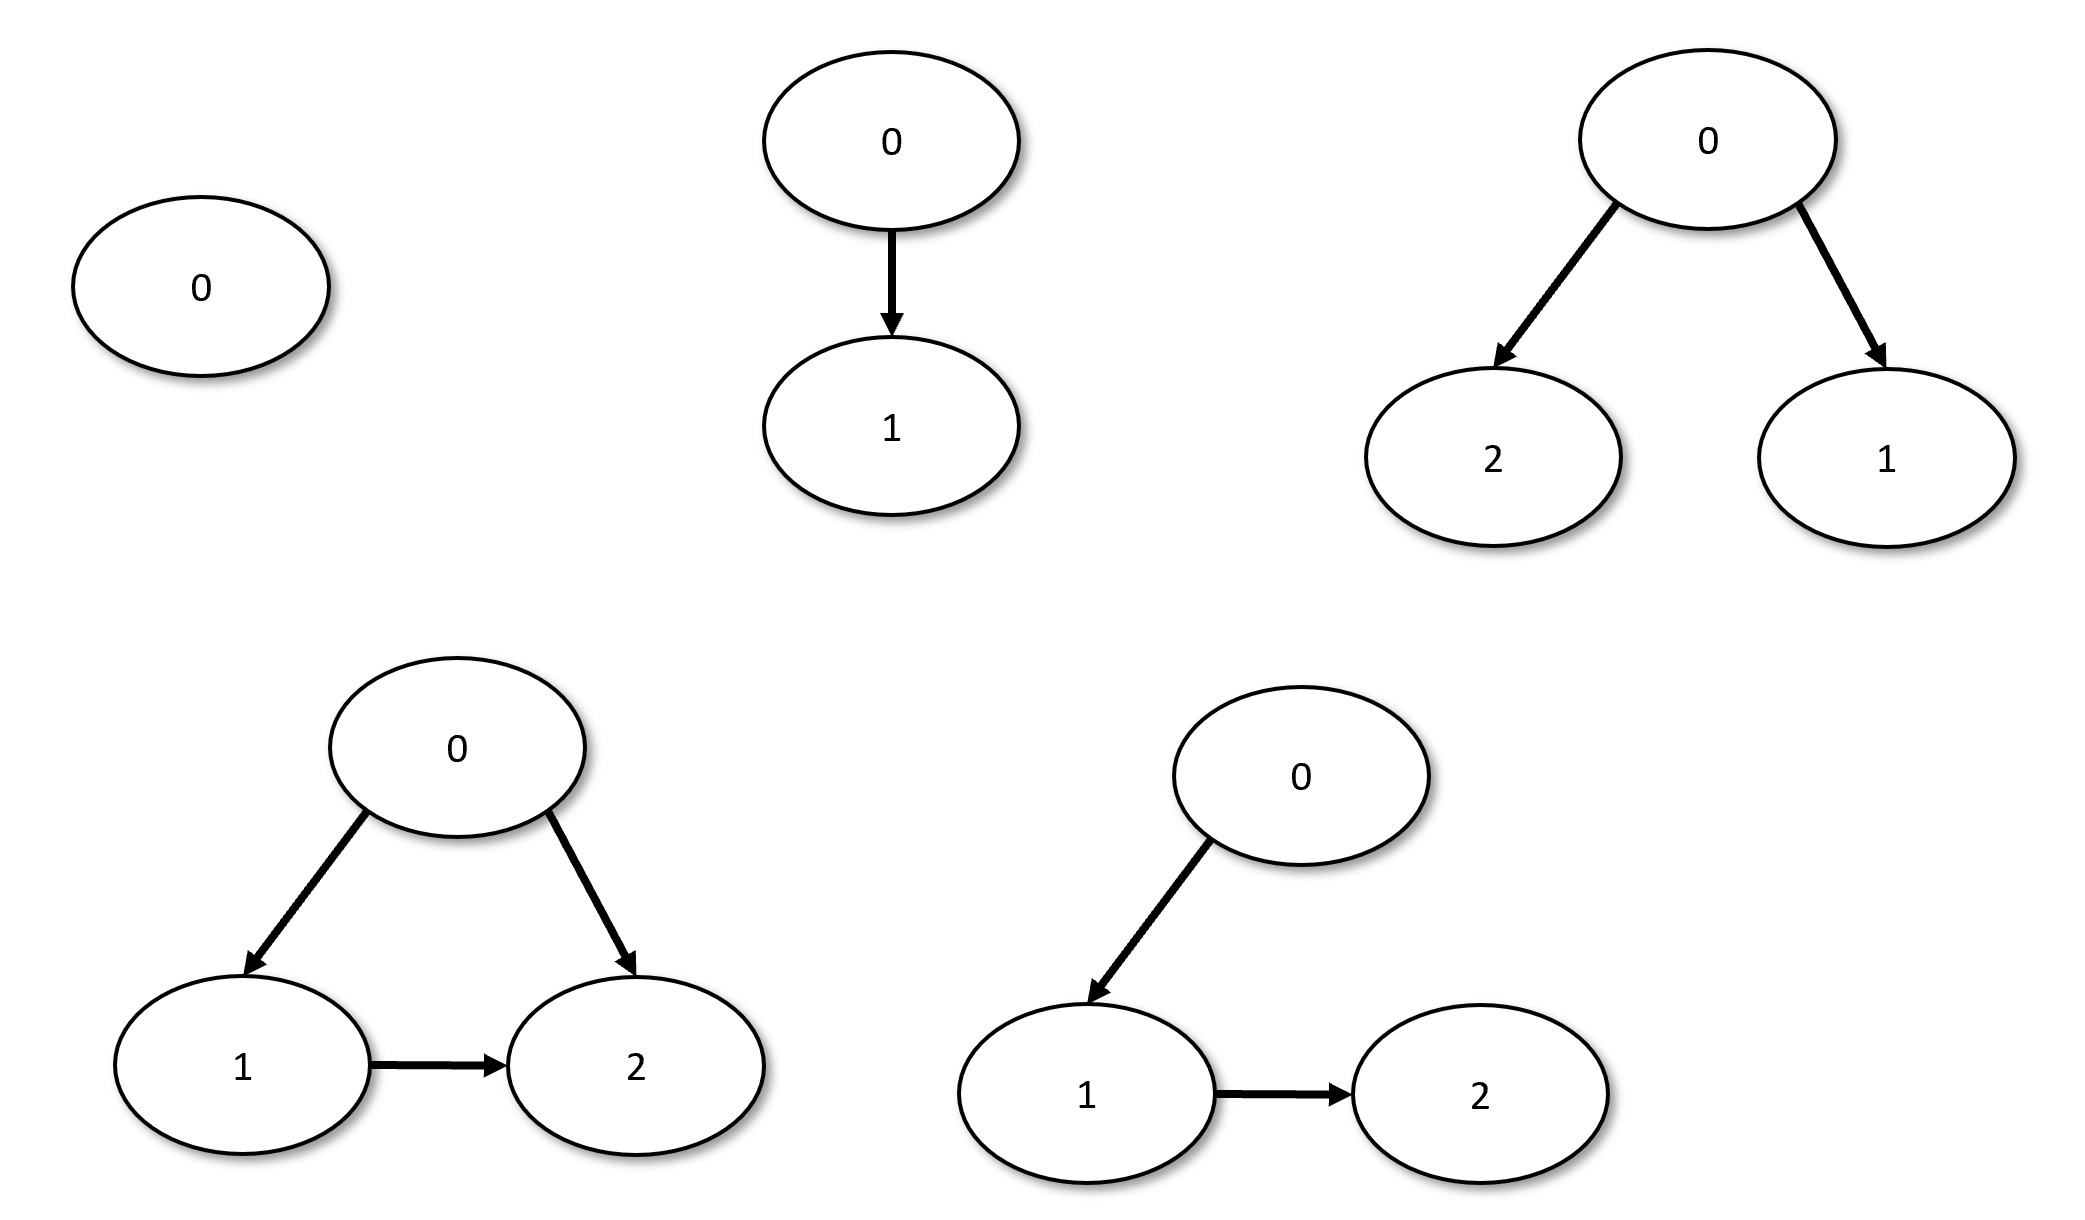
\includegraphics[width=\linewidth, height=1.5in, keepaspectratio]{../figure/topologicalsortexamples.png}
\caption{Some examples of DAGs of one, two and three vertices, and valid
ways to assign layers to the vertices.}
\label{topsortexamplesfig}
\end{marginfigure}

\emph{Induction} is simply an application of the self-evident
\href{https://en.wikipedia.org/wiki/Modus_ponens}{Modus Ponens rule}
that says that if

\paragraph{(a)} \(P\) is true

and

\paragraph{(b)} \(P\) implies \(Q\)

then \(Q\) is true.

In the setting of proofs by induction we typically have a statement
\(Q(k)\) that is parameterized by some integer \(k\), and we prove that
\textbf{(a)} \(Q(0)\) is true, and \textbf{(b)} For every \(k>0\), if
\(Q(0),\ldots,Q(k-1)\) are all true then \(Q(k)\) is true. (Usually
proving \textbf{(b)} is the hard part, though there are examples where
the ``base case'' \textbf{(a)} is quite subtle.) By applying Modus
Ponens, we can deduce from \textbf{(a)} and \textbf{(b)} that \(Q(1)\)
is true. Once we did so, since we now know that both \(Q(0)\) and
\(Q(1)\) are true, then we can use this and \textbf{(b)} to deduce
(again using Modus Ponens) that \(Q(2)\) is true. We can repeat the same
reasoning again and again to obtain that \(Q(k)\) is true for every
\(k\). The statement \textbf{(a)} is called the ``base case'', while
\textbf{(b)} is called the ``inductive step''. The assumption in
\textbf{(b)} that \(Q(i)\) holds for \(i<k\) is called the ``inductive
hypothesis''. (The form of induction described here is sometimes called
``strong induction'' as opposed to ``weak induction'' where we replace
\textbf{(b)} by the statement \textbf{(b')} that if \(Q(k-1)\) is true
then \(Q(k)\) is true; weak induction can be thought of as the special
case of strong induction where we don't use the assumption that
\(Q(0),\ldots,Q(k-2)\) are true.)

\hypertarget{inducrecrem}{}
\begin{remark}[Induction and recursion] \label[remark]{inducrecrem}

Proofs by induction are closely related to algorithms by recursion. In
both cases we reduce solving a larger problem to solving a smaller
instance of itself. In a recursive algorithm to solve some problem P on
an input of length \(k\) we ask ourselves ``what if someone handed me a
way to solve P on instances smaller than \(k\)?''. In an inductive proof
to prove a statement Q parameterized by a number \(k\), we ask ourselves
``what if I already knew that \(Q(k')\) is true for \(k'<k\)?''. Both
induction and recursion are crucial concepts for this course and
Computer Science at large (and even other areas of inquiry, including
not just mathematics but other sciences as well). Both can be confusing
at first, but with time and practice they become clearer. For more on
proofs by induction and recursion, you might find the following
\href{https://cs121.boazbarak.org/StanfordCS103Induction.pdf}{Stanford
CS 103 handout},
\href{https://ocw.mit.edu/courses/electrical-engineering-and-computer-science/6-00sc-introduction-to-computer-science-and-programming-spring-2011/unit-1/lecture-6-recursion/}{this
MIT 6.00 lecture} or
\href{https://cs121.boazbarak.org/LL_induction.pdf}{this excerpt of the
Lehman-Leighton book} useful.

\end{remark}

\subsection{Proving the result by
induction}\label{Proving-the-result-by-ind}

There are several ways to use induction to prove \cref{acyclictosortlem}
by induction. We will use induction on the number \(n\) of vertices, and
so we will define the statement \(Q(n)\) as follows:

\begin{quote}
\(Q(n)\) is \emph{``For every DAG \(G=(V,E)\) with \(n\) vertices, there
is a layering of \(G\).''}
\end{quote}

The statement for \(Q(0)\) (where the graph contains no vertices) is
trivial. Thus it will suffice to prove the following: \emph{for every
\(n>0\), if \(Q(n-1)\) is true then \(Q(n)\) is true.}

To do so, we need to somehow find a way, given a graph \(G\) of \(n\)
vertices, to reduce the task of finding a layering for \(G\) into the
task of finding a layering for some other graph \(G'\) of \(n-1\)
vertices. The idea is that we will find a \emph{source} of \(G\): a
vertex \(v\) that has no in-neighbors. We can then assign to \(v\) the
layer \(0\), and layer the remaining vertices using the inductive
hypothesis in layers \(1,2,\ldots\).

The above is the intuition behind the proof of \cref{acyclictosortlem},
but when writing the formal proof below, we use the benefit of
hindsight, and try to streamline what was a messy journey into a linear
and easy-to-follow flow of logic that starts with the word
\textbf{``Proof:''} and ends with \textbf{``QED''} or the symbol
\(\blacksquare\).\footnote{QED stands for ``quod erat demonstrandum'',
  which is Latin for ``what was to be demonstrated'' or ``the very thing
  it was required to have shown''.} Discussions, examples and
digressions can be very insightful, but we keep them outside the space
delimited between these two words, where (as described by this
\href{http://web.stanford.edu/class/cs103/handouts/120\%20Proofwriting\%20Checklist.pdf}{excellent
handout}) ``every sentence must be load bearing''. Just like we do in
programming, we can break the proof into little ``subroutines'' or
``functions'' (known as \emph{lemmas} or \emph{claims} in math
language), which will be smaller statements that help us prove the main
result. However, the proof should be structured in a way that ensures
that it is always crystal-clear to the reader in what stage we are of
the proof. The reader should be able to tell what is the role of every
sentence in the proof and which part it belongs to. We now present the
formal proof of \cref{acyclictosortlem}.

\begin{proof}[Proof of \cref{acyclictosortlem}] \label[proof]{Let-GVE-be-a-DAG-and-nV-b}

Let \(G=(V,E)\) be a DAG and \(n=|V|\) be the number of its vertices. We
prove the lemma by induction on \(n\). The base case is \(n=0\) where
there are no vertices, and so the statement is trivially true.\footnote{Using
  \(n=0\) as the base case is logically valid, but can be confusing. If
  you find the trivial \(n=0\) case to be confusing, you can always
  directly verify the statement for \(n=1\) and then use both \(n=0\)
  and \(n=1\) as the base cases.} For the case of \(n>0\), we make the
inductive hypothesis that every DAG \(G'\) of at most \(n-1\) vertices
has a layering.

We make the following claim:

\textbf{Claim:} \(G\) must contain a vertex \(v\) of in-degree zero.

\textbf{Proof of Claim:} Suppose otherwise that every vertex \(v\in V\)
has an in-neighbor. Let \(v_0\) be some vertex of \(G\), let \(v_1\) be
an in-neighbor of \(v_0\), \(v_2\) be an in-neighbor of \(v_1\), and
continue in this way for \(n\) steps until we construct a list
\(v_0,v_1,\ldots,v_n\) such that for every \(i\in [n]\), \(v_{i+1}\) is
an in-neighbor of \(v_i\), or in other words the edge
\(v_{i+1} \rightarrow v_i\) is present in the graph. Since there are
only \(n\) vertices in this graph, one of the \(n+1\) vertices in this
sequence must repeat itself, and so there exists \(i<j\) such that
\(v_i=v_j\). But then the sequence
\(v_j \rightarrow v_{j-1} \rightarrow \cdots \rightarrow v_i\) is a
cycle in \(G\), contradicting our assumption that it is acyclic.
\textbf{(QED Claim)}

Given the claim, we can let \(v_0\) be some vertex of in-degree zero in
\(G\), and let \(G'\) be the graph obtained by removing \(v_0\) from
\(G\). \(G'\) has \(n-1\) vertices and hence per the inductive
hypothesis has a layering \(f':(V \setminus \{v_0\}) \rightarrow \N\).
We define \(f:V \rightarrow \N\) as follows:

\[f(v) = \begin{cases}f'(v)+1 & v \neq v_0 \\ 0 & v=v_0 \end{cases}\;.\]

We claim that \(f\) is a valid layering, namely that for every edge
\(u \rightarrow v\), \(f(u) < f(v)\). To prove this, we split into
cases:

\begin{itemize}
\item
  \textbf{Case 1:} \(u \neq v_0\), \(v \neq v_0\). In this case the edge
  \(u \rightarrow v\) exists in the graph \(G'\) and hence by the
  inductive hypothesis \(f'(u) < f'(v)\) which implies that
  \(f'(u)+1 < f'(v)+1\).
\item
  \textbf{Case 2:} \(u=v_0\), \(v \neq v_0\). In this case \(f(u)=0\)
  and \(f(v) = f'(v)+1>0\).
\item
  \textbf{Case 3:} \(u \neq v_0\), \(v=v_0\). This case can't happen
  since \(v_0\) does not have in-neighbors.
\item
  \textbf{Case 4:} \(u=v_0, v=v_0\). This case again can't happen since
  it means that \(v_0\) is its own-neighbor --- it is involved in a
  \emph{self loop} which is a form cycle that is disallowed in an
  acyclic graph.
\end{itemize}

Thus, \(f\) is a valid layering for \(G\) which completes the proof.

\end{proof}

\begin{pause} \label[pause]{Reading-a-proof-is-no-les}

Reading a proof is no less of an important skill than producing one. In
fact, just like understanding code, it is a highly non-trivial skill in
itself. Therefore I strongly suggest that you re-read the above proof,
asking yourself at every sentence whether the assumption it makes is
justified, and whether this sentence truly demonstrates what it purports
to achieve. Another good habit is to ask yourself when reading a proof
for every variable you encounter (such as \(u\), \(i\), \(G'\), \(f'\),
etc. in the above proof) the following questions: \textbf{(1)} What
\emph{type} of variable is it? is it a number? a graph? a vertex? a
function? and \textbf{(2)} What do we know about it? Is it an arbitrary
member of the set? Have we shown some facts about it?, and \textbf{(3)}
What are we \emph{trying} to show about it?.

\end{pause}

\subsection{Minimality and uniqueness}\label{Minimality-and-uniqueness}

\cref{topologicalsortthm} guarantees that for every DAG \(G=(V,E)\)
there exists some layering \(f:V \rightarrow \N\) but this layering is
not necessarily \emph{unique}. For example, if \(f:V \rightarrow \N\) is
a valid layering of the graph then so is the function \(f'\) defined as
\(f'(v) = 2\cdot f(v)\). However, it turns out that the \emph{minimal}
layering is unique. A minimal layering is one where every vertex is
given the smallest layer number possible. We now formally define
minimality and state the uniqueness theorem:

\hypertarget{minimallayeruniquethm}{}
\begin{theorem}[Minimal layering is unique] \label[theorem]{minimallayeruniquethm}

Let \(G=(V,E)\) be a DAG. We say that a layering \(f:V \rightarrow \N\)
is \emph{minimal} if for every vertex \(v \in V\), if \(v\) has no
in-neighbors then \(f(v)=0\) and if \(v\) has in-neighbors then there
exists an in-neighbor \(u\) of \(v\) such that \(f(u) = f(v)-1\).

For every layering \(f,g:V \rightarrow \N\) of \(G\), if both \(f\) and
\(g\) are minimal then \(f=g\).

\end{theorem}

The definition of minimality in \cref{minimallayeruniquethm} implies
that for every vertex \(v \in V\), we cannot move it to a lower layer
without making the layering invalid. If \(v\) is a source (i.e., has
in-degree zero) then a minimal layering \(f\) must put it in layer
\(0\), and for every other \(v\), if \(f(v)=i\), then we cannot modify
this to set \(f(v) \leq i-1\) since there is an-neighbor \(u\) of \(v\)
satisfying \(f(u)=i-1\). What \cref{minimallayeruniquethm} says is that
a minimal layering \(f\) is \emph{unique} in the sense that every other
minimal layering is equal to \(f\).

\begin{proofidea} \label[proofidea]{The-idea-is-to-prove-the-}

The idea is to prove the theorem by induction on the layers. If \(f\)
and \(g\) are minimal then they must agree on the source vertices, since
both \(f\) and \(g\) should assign these vertices to layer \(0\). We can
then show that if \(f\) and \(g\) agree up to layer \(i-1\), then the
minimality property implies that they need to agree in layer \(i\) as
well. In the actual proof we use a small trick to save on writing.
Rather than proving the statement that \(f=g\) (or in other words that
\(f(v)=g(v)\) for every \(v\in V\)), we prove the weaker statement that
\(f(v) \leq g(v)\) for every \(v\in V\). (This is a weaker statement
since the condition that \(f(v)\) is lesser or equal than to \(g(v)\) is
implied by the condition that \(f(v)\) is equal to \(g(v)\).) However,
since \(f\) and \(g\) are just labels we give to two minimal layerings,
by simply changing the names ``\(f\)'' and ``\(g\)'' the same proof also
shows that \(g(v) \leq f(v)\) for every \(v\in V\) and hence that
\(f=g\).

\end{proofidea}

\begin{proof}[Proof of \cref{minimallayeruniquethm}] \label[proof]{Let-GVE-be-a-DAG-and-fgV-}

Let \(G=(V,E)\) be a DAG and \(f,g:V \rightarrow \N\) be two minimal
valid layering of \(G\). We will prove that for every \(v \in V\),
\(f(v) \leq g(v)\). Since we didn't assume anything about \(f,g\) except
their minimality, the same proof will imply that for every \(v\in V\),
\(g(v) \leq f(v)\) and hence that \(f(v)=g(v)\) for every \(v\in V\),
which is what we needed to show.

We will prove that \(f(v) \leq g(v)\) for every \(v \in V\) by induction
on \(i = f(v)\). The case \(i=0\) is immediate: since in this case
\(f(v)=0\), \(g(v)\) must be at least \(f(v)\). For the case \(i>0\), by
the minimality of \(f\), if \(f(v)=i\) then there must exist some
in-neighbor \(u\) of \(v\) such that \(f(u) = i-1\). By the induction
hypothesis we get that \(g(u) \geq i-1\), and since \(g\) is a valid
layering it must hold that \(g(v) > g(u)\) which means that
\(g(v) \geq i = f(v)\).

\end{proof}

\begin{pause} \label[pause]{The-proof-of-crefminimall}

The proof of \cref{minimallayeruniquethm} is fully rigorous, but is
written in a somewhat terse manner. Make sure that you read through it
and understand \emph{why} this is indeed an airtight proof of the
Theorem's statement.

\end{pause}

\section{This book: notation and conventions}\label{notationsec}

Most of the notation we use in this book is standard and is used in most
mathematical texts. The main points where we diverge are:

\begin{itemize}
\item
  We index the natural numbers \(\N\) starting with \(0\) (though many
  other texts, especially in computer science, do the same).
\item
  We also index the set \([n]\) starting with \(0\), and hence define it
  as \(\{0,\ldots,n-1\}\). In other texts it is often defined as
  \(\{1,\ldots, n \}\). Similarly, we index our strings starting with
  \(0\), and hence a string \(x\in \{0,1\}^n\) is written as
  \(x_0x_1\cdots x_{n-1}\).
\item
  If \(n\) is a natural number then \(1^n\) does \emph{not} equal the
  number \(1\) but rather this is the length \(n\) string \(11\cdots 1\)
  (that is a string of \(n\) ones). Similarly, \(0^n\) refers to the
  length \(n\) string \(00 \cdots 0\).
\item
  \emph{Partial} functions are functions that are not necessarily
  defined on all inputs. When we write \(f:A \rightarrow B\) this means
  that \(f\) is a \emph{total} function unless we say otherwise. When we
  want to emphasize that \(f\) can be a partial function, we will
  sometimes write \(f: A \rightarrow_p B\).
\item
  As we will see later on in the course, we will mostly describe our
  computational problems in terms of computing a \emph{Boolean function}
  \(f: \{0,1\}^* \rightarrow \{0,1\}\). In contrast, many other
  textbooks refer to the same task as \emph{deciding a language}
  \(L \subseteq \{0,1\}^*\). These two viewpoints are equivalent, since
  for every set \(L\subseteq \{0,1\}^*\) there is a corresponding
  function \(F\) such that \(F(x)=1\) if and only if \(x\in L\).
  Computing \emph{partial functions} corresponds to the task known in
  the literature as a solving a \emph{promise problem}. Because the
  language notation is so prevalent in other textbooks, we will
  occasionally remind the reader of this correspondence.
\item
  We use \(\ceil{x}\) and \(\floor{x}\) for the ``ceiling'' and
  ``floor'' operators that correspond to ``rounding up'' or ``rounding
  down'' a number to the nearest integer. We use \((x \mod y)\) to
  denote the ``remainder'' of \(x\) when divided by \(y\). That is,
  \((x \mod y) = x - y\floor{x/y}\). In context when an integer is
  expected we'll typically ``silently round'' the quantities to an
  integer. For example, if we say that \(x\) is a string of length
  \(\sqrt{n}\) then this means that \(x\) is of length
  \(\lceil \sqrt{n}\, \rceil\). (We round up for the sake of convention,
  but in most such cases, it will not make a difference whether we round
  up or down.)
\item
  Like most Computer Science texts, we default to the logarithm in base
  two. Thus, \(\log n\) is the same as \(\log_2 n\).
\item
  We will also use the notation \(f(n)=poly(n)\) as a shorthand for
  \(f(n)=n^{O(1)}\) (i.e., as shorthand for saying that there are some
  constants \(a,b\) such that \(f(n) \leq a\cdot n^b\) for every
  sufficiently large \(n\)). Similarly, we will use \(f(n)=polylog(n)\)
  as shorthand for \(f(n)=poly(\log n)\) (i.e., as shorthand for saying
  that there are some constants \(a,b\) such that
  \(f(n) \leq a\cdot (\log n)^b\) for every sufficiently large \(n\)).
\item
  As in often the case in mathematical literature, we use the apostrophe
  character to enrich our set of identifiers. Typically if \(x\) denotes
  some object, then \(x'\), \(x''\), etc. will denote other objects of
  the same type.
\item
  To save on ``cognitive load'' we will often use round constants such
  as \(10,100,1000\) in the statements of both theorems and problem set
  questions. When you see such a ``round'' constant, you can typically
  assume that it has no special significance and was just chosen
  arbitrarily. For example, if you see a theorem of the form ``Algorithm
  \(A\) takes at most \(1000\cdot n^2\) steps to compute function \(F\)
  on inputs of length \(n\)'' then probably the number \(1000\) is an
  abitrary sufficiently large constant, and one could prove the same
  theorem with a bound of the form \(c \cdot n^2\) for a constant \(c\)
  that is smaller than \(1000\). Similarly, if a problem asks you to
  prove that some quantity is at least \(n/100\), it is quite possible
  that in truth the quantity is at least \(n/d\) for some constant \(d\)
  that is smaller than \(100\).
\end{itemize}

\subsection{Variable name conventions}\label{conventionsec}

Like programming, mathematics is full of \emph{variables}. Whenever you
see a variable, it is always important to keep track of what is its
\emph{type} (e.g., whether the variable is a number, a string, a
function, a graph, etc.). To make this easier, we try to stick to
certain conventions and consistently use certain identifiers for
variables of the same type. Some of these conventions are listed in
\cref{notationtable} below. These conventions are not immutable laws and
we might occasionally deviate from them. Also, such conventions do not
replace the need to explicitly declare for each new variable the type of
object that it denotes.

\begin{longtable}[]{@{}ll@{}}
\caption{Conventions for identifiers in this book}\tabularnewline
\toprule
\begin{minipage}[b]{0.11\columnwidth}\raggedright
\emph{Identifier}\strut
\end{minipage} & \begin{minipage}[b]{0.83\columnwidth}\raggedright
\emph{Often denotes object of type}\strut
\end{minipage}\tabularnewline
\midrule
\endfirsthead
\toprule
\begin{minipage}[b]{0.11\columnwidth}\raggedright
\emph{Identifier}\strut
\end{minipage} & \begin{minipage}[b]{0.83\columnwidth}\raggedright
\emph{Often denotes object of type}\strut
\end{minipage}\tabularnewline
\midrule
\endhead
\begin{minipage}[t]{0.11\columnwidth}\raggedright
\(i\),\(j\),\(k\),\(\ell\),\(m\),\(n\)\strut
\end{minipage} & \begin{minipage}[t]{0.83\columnwidth}\raggedright
Natural numbers (i.e., in \(\mathbb{N} = \{0,1,2,\ldots \}\))\strut
\end{minipage}\tabularnewline
\begin{minipage}[t]{0.11\columnwidth}\raggedright
\(\epsilon,\delta\)\strut
\end{minipage} & \begin{minipage}[t]{0.83\columnwidth}\raggedright
Small positive real numbers (very close to \(0\))\strut
\end{minipage}\tabularnewline
\begin{minipage}[t]{0.11\columnwidth}\raggedright
\(x,y,z,w\)\strut
\end{minipage} & \begin{minipage}[t]{0.83\columnwidth}\raggedright
Typically strings in \(\{0,1\}^*\) though sometimes numbers or other
objects. We often identify an object with its representation as a
string.\strut
\end{minipage}\tabularnewline
\begin{minipage}[t]{0.11\columnwidth}\raggedright
\(G\)\strut
\end{minipage} & \begin{minipage}[t]{0.83\columnwidth}\raggedright
A \emph{graph}. The set of \(G\)'s vertices is typically denoted by
\(V\). Often \(V=[n]\). The set of \(G\)'s edges is typically denoted by
\(E\).\strut
\end{minipage}\tabularnewline
\begin{minipage}[t]{0.11\columnwidth}\raggedright
\(S\)\strut
\end{minipage} & \begin{minipage}[t]{0.83\columnwidth}\raggedright
Set\strut
\end{minipage}\tabularnewline
\begin{minipage}[t]{0.11\columnwidth}\raggedright
\(f,g,h\)\strut
\end{minipage} & \begin{minipage}[t]{0.83\columnwidth}\raggedright
Functions. We often (though not always) use lowercase identifiers for
\emph{finite functions}, which map \(\{0,1\}^n\) to \(\{0,1\}^m\) (often
\(m=1\)).\strut
\end{minipage}\tabularnewline
\begin{minipage}[t]{0.11\columnwidth}\raggedright
\(F,G,H\)\strut
\end{minipage} & \begin{minipage}[t]{0.83\columnwidth}\raggedright
Infinite (unbounded input) functions mapping \(\{0,1\}^*\) to
\(\{0,1\}^*\) or \(\{0,1\}^*\) to \(\{0,1\}^m\) for some \(m\). Based on
context, the identifiers \(G,H\) are sometimes used to denote functions
and sometimes graphs.\strut
\end{minipage}\tabularnewline
\begin{minipage}[t]{0.11\columnwidth}\raggedright
\(A,B,C\)\strut
\end{minipage} & \begin{minipage}[t]{0.83\columnwidth}\raggedright
Boolean circuits\strut
\end{minipage}\tabularnewline
\begin{minipage}[t]{0.11\columnwidth}\raggedright
\(M,N\)\strut
\end{minipage} & \begin{minipage}[t]{0.83\columnwidth}\raggedright
Turing machines\strut
\end{minipage}\tabularnewline
\begin{minipage}[t]{0.11\columnwidth}\raggedright
\(P,Q\)\strut
\end{minipage} & \begin{minipage}[t]{0.83\columnwidth}\raggedright
Programs\strut
\end{minipage}\tabularnewline
\begin{minipage}[t]{0.11\columnwidth}\raggedright
\(T\)\strut
\end{minipage} & \begin{minipage}[t]{0.83\columnwidth}\raggedright
A function mapping \(\mathbb{N}\) to \(\mathbb{N}\) that corresponds to
a time bound.\strut
\end{minipage}\tabularnewline
\begin{minipage}[t]{0.11\columnwidth}\raggedright
\(c\)\strut
\end{minipage} & \begin{minipage}[t]{0.83\columnwidth}\raggedright
A positive number (often an unspecified constant; e.g., \(T(n)=O(n)\)
corresponds to the existence of \(c\) s.t. \(T(n) \leq c \cdot n\) every
\(n>0\)). We sometimes use \(a,b\) in a similar way.\strut
\end{minipage}\tabularnewline
\begin{minipage}[t]{0.11\columnwidth}\raggedright
\(\Sigma\)\strut
\end{minipage} & \begin{minipage}[t]{0.83\columnwidth}\raggedright
Finite set (often used as the \emph{alphabet} for a set of
strings).\strut
\end{minipage}\tabularnewline
\bottomrule
\end{longtable}

\label{notationtable}

\subsection{Some idioms}\label{Some-idioms}

Mathematical texts often employ certain conventions or ``idioms''. Some
examples of such idioms that we use in this text include the following:

\begin{itemize}
\item
  \textbf{``Let \(X\) be \(\ldots\)''}, \textbf{``let \(X\) denote
  \(\ldots\)''}, or \textbf{``let \(X= \ldots\)'':} These are all
  different ways for us to say that we are \emph{defining} the symbol
  \(X\) to stand for whatever expression is in the \(\ldots\). When
  \(X\) is a \emph{property} of some objects we might define \(X\) by
  writing something along the lines of \textbf{``We say that \(\ldots\)
  has the property \(X\) if \(\ldots\).''}. While we often try to define
  terms before they are used, sometimes a mathematical sentence reads
  easier if we use a term before defining it, in which case we add
  \textbf{``Where \(X\) is \(\ldots\)''} to explain how \(X\) is defined
  in the preceding expression.
\item
  \textbf{Quantifiers:} Mathematical texts involve many quantifiers such
  as ``for all'' and ``exists''. We sometimes spell these in words as in
  \textbf{``for all \(i\in\N\)''} or \textbf{``there is
  \(x\in \{0,1\}^*\)''}, and sometimes use the formal symbols
  \(\forall\) and \(\exists\). It is important to keep track on which
  variable is quantified in what way the \emph{dependencies} between the
  variables. For example, a sentence fragment such as \textbf{``for
  every \(k >0\) there exists \(n\)''} means that \(n\) can be chosen in
  a way that \emph{depends} on \(k\). The order of quantifiers is
  important. For example, the following is a true statement: \emph{``for
  every natural number \(k>1\) there exists a prime number \(n\) such
  that \(n\) divides \(k\).''} In contrast, the following statement is
  false: \emph{``there exists a prime number \(n\) such that for every
  natural number \(k>1\), \(n\) divides \(k\).''}
\item
  \textbf{Numbered equations, theorems, definitions:} To keep track of
  all the terms we define and statements we prove, we often assign them
  a (typically numeric) label, and then refer back to them in other
  parts of the text.
\item
  \textbf{(i.e.,), (e.g.,):} Mathematical texts tend to contain quite a
  few of these expressions. We use \(X\) (i.e., \(Y\)) in cases where
  \(Y\) is equivalent to \(X\) and \(X\) (e.g., \(Y\)) in cases where
  \(Y\) is an example of \(X\) (e.g., one can use phrases such as ``a
  natural number (i.e., a non-negative integer)'' or ``a natural number
  (e.g., \(7\))'').
\item
  \textbf{``Thus''}, \textbf{``Therefore''} , \textbf{``We get that''}:
  This means that the following sentence is implied by the preceding
  one, as in ``The \(n\)-vertex graph \(G\) is connected. Therefore it
  contains at least \(n-1\) edges.'' We sometimes use
  \textbf{``indeed''} to indicate that the following text justifies the
  claim that was made in the preceding sentence as in \emph{``The
  \(n\)-vertex graph \(G\) has at least \(n-1\) edges. Indeed, this
  follows since \(G\) is connected.''}
\item
  \textbf{Constants:} In Computer Science, we typically care about how
  our algorithms' resource consumption (such as running time)
  \emph{scales} with certain quantities (such as the length of the
  input). We refer to quantities that do not depend on the length of the
  input as \emph{constants} and so often use statements such as
  \emph{``there exists a constant \(c>0\) such that for every
  \(n\in \N\), Algorithm \(A\) runs in at most \(c \cdot n^2\) steps on
  inputs of length \(n\).''} The qualifier ``constant'' for \(c\) is not
  strictly needed but is added to emphasize that \(c\) here is a fixed
  number independent of \(n\). In fact sometimes, to reduce cognitive
  load, we will simply replace \(c\) by a sufficiently large round
  number such as \(10\), \(100\), or \(1000\), or use \(O\)-notation and
  write \emph{``Algorithm \(A\) runs in \(O(n^2)\) time.''}
\end{itemize}

\begin{recap} \label[recap]{The-basic-mathematical-da}

\begin{itemize}
\tightlist
\item
  The basic ``mathematical data structures'' we'll need are
  \emph{numbers}, \emph{sets}, \emph{tuples}, \emph{strings},
  \emph{graphs} and \emph{functions}.
\item
  We can use basic objects to define more complex notions. For example,
  \emph{graphs} can be defined as a list of \emph{pairs}.
\item
  Given precise \emph{definitions} of objects, we can state unambiguous
  and precise \emph{statements}. We can then use mathematical
  \emph{proofs} to determine whether these statements are true or false.
\item
  A mathematical proof is not a formal ritual but rather a clear,
  precise and ``bulletproof'' argument certifying the truth of a certain
  statement.
\item
  Big-\(O\) notation is an extremely useful formalism to suppress less
  significant details and allow us to focus on the high level behavior
  of quantities of interest.
\item
  The only way to get comfortable with mathematical notions is to apply
  them in the contexts of solving problems. You should expect to need to
  go back time and again to the definitions and notation in this chapter
  as you work through problems in this course.
\end{itemize}

\end{recap}

\section{Exercises}\label{Exercises}

\hypertarget{logicalex}{}
\begin{exercise}[Logical expressions] \label[exercise]{logicalex}

\begin{enumerate}
\def\labelenumi{\alph{enumi}.}
\item
  Write a logical expression \(\varphi(x)\) involving the variables
  \(x_0,x_1,x_2\) and the operators \(\wedge\) (AND), \(\vee\) (OR), and
  \(\neg\) (NOT), such that \(\varphi(x)\) is true if the majority of
  the inputs are \emph{True}.
\item
  Write a logical expression \(\varphi(x)\) involving the variables
  \(x_0,x_1,x_2\) and the operators \(\wedge\) (AND), \(\vee\) (OR), and
  \(\neg\) (NOT), such that \(\varphi(x)\) is true if the sum
  \(\sum_{i=0}^{2} x_i\) (identifying ``true'' with \(1\) and ``false''
  with \(0\)) is \emph{odd}.
\end{enumerate}

\end{exercise}

\hypertarget{quantifiersex}{}
\begin{exercise}[Quantifiers] \label[exercise]{quantifiersex}

Use the logical quantifiers \(\forall\) (for all), \(\exists\) (there
exists), as well as \(\wedge,\vee,\neg\) and the arithmetic operations
\(+,\times,=,>,<\) to write the following:

\begin{enumerate}
\def\labelenumi{\alph{enumi}.}
\item
  An expression \(\varphi(n,k)\) such that for every natural numbers
  \(n,k\), \(\varphi(n,k)\) is true if and only if \(k\) divides \(n\).
\item
  An expression \(\varphi(n)\) such that for every natural number \(n\),
  \(\varphi(n)\) is true if and only if \(n\) is a power of three.
\end{enumerate}

\end{exercise}

\begin{exercise} \label[exercise]{Describe-the-following-st}

Describe the following statement in English words:
\(\forall_{n\in\N} \exists_{p>n} \forall{a,b \in \N} (a\times b \neq p) \vee (a=1)\).

\end{exercise}

\hypertarget{setsdescription}{}
\begin{exercise}[Set construction notation] \label[exercise]{setsdescription}

Describe in words the following sets:

\begin{enumerate}
\def\labelenumi{\alph{enumi}.}
\item
  \(S = \{ x\in \{0,1\}^{100} : \forall_{i\in \{0,\ldots, 99\}} x_i = x_{99-i} \}\)
\item
  \(T = \{ x\in \{0,1\}^* : \forall_{i,j \in \{2,\ldots,|x|-1 \} } i\cdot j \neq |x| \}\)
\end{enumerate}

\end{exercise}

\hypertarget{cardinalitiesex}{}
\begin{exercise}[Existence of one to one mappings] \label[exercise]{cardinalitiesex}

For each one of the following pairs of sets \((S,T)\), prove or disprove
the following statement: there is a one to one function \(f\) mapping
\(S\) to \(T\).

\begin{enumerate}
\def\labelenumi{\alph{enumi}.}
\item
  Let \(n>10\). \(S = \{0,1\}^n\) and \(T= [n] \times [n] \times [n]\).
\item
  Let \(n>10\). \(S\) is the set of all functions mapping \(\{0,1\}^n\)
  to \(\{0,1\}\). \(T = \{0,1\}^{n^3}\).
\item
  Let \(n>100\). \(S = \{k \in [n] \;|\; k \text{ is prime} \}\),
  \(T = \{0,1\}^{\ceil{\log n -1}}\).
\end{enumerate}

\end{exercise}

\hypertarget{inclex}{}
\begin{exercise}[Inclusion Exclusion] \label[exercise]{inclex}

\begin{enumerate}
\def\labelenumi{\alph{enumi}.}
\item
  Let \(A,B\) be finite sets. Prove that
  \(|A\cup B| = |A|+|B|-|A\cap B|\).
\item
  Let \(A_0,\ldots,A_{k-1}\) be finite sets. Prove that
  \(|A_0 \cup \cdots \cup A_{k-1}| \geq \sum_{i=0}^{k-1} |A_i| - \sum_{0 \leq i < j < k} |A_i \cap A_j|\).
\item
  Let \(A_0,\ldots,A_{k-1}\) be finite subsets of \(\{1,\ldots, n\}\),
  such that \(|A_i|=m\) for every \(i\in [k]\). Prove that if
  \(k>100n\), then there exist two distinct sets \(A_i,A_j\) s.t.
  \(|A_i \cap A_j| \geq m^2/(10n)\).
\end{enumerate}

\end{exercise}

\begin{exercise} \label[exercise]{Prove-that-if-ST-are-fini}

Prove that if \(S,T\) are finite and \(F:S \rightarrow T\) is one to one
then \(|S| \leq |T|\).

\end{exercise}

\begin{exercise} \label[exercise]{Prove-that-if-ST-are-fini}

Prove that if \(S,T\) are finite and \(F:S \rightarrow T\) is onto then
\(|S| \geq |T|\).

\end{exercise}

\begin{exercise} \label[exercise]{Prove-that-for-every-fini}

Prove that for every finite \(S,T\), there are \((|T|+1)^{|S|}\) partial
functions from \(S\) to \(T\).

\end{exercise}

\begin{exercise} \label[exercise]{Suppose-that--Sn-nin-N-is}

Suppose that \(\{ S_n \}_{n\in \N}\) is a sequence such that
\(S_0 \leq 10\) and for \(n>1\)
\(S_n \leq 5 S_{\lfloor \tfrac{n}{5} \rfloor} + 2n\). Prove by induction
that \(S_n \leq 100 n \log n\) for every \(n\).

\end{exercise}

\begin{exercise} \label[exercise]{Prove-that-for-every-undi}

Prove that for every undirected graph \(G\) of \(100\) vertices, if
every vertex has degree at most \(4\), then there exists a subset \(S\)
of at \(20\) vertices such that no two vertices in \(S\) are neighbors
of one another.

\end{exercise}

\hypertarget{ohnotationex}{}
\begin{exercise}[$O$-notation] \label[exercise]{ohnotationex}

For every pair of functions \(F,G\) below, determine which of the
following relations holds: \(F=O(G)\), \(F=\Omega(G)\), \(F=o(G)\) or
\(F=\omega(G)\).

\begin{enumerate}
\def\labelenumi{\alph{enumi}.}
\item
  \(F(n)=n\), \(G(n)=100n\).
\item
  \(F(n)=n\), \(G(n)=\sqrt{n}\).
\item
  \(F(n)=n\log n\), \(G(n)=2^{(\log (n))^2}\).
\item
  \(F(n)=\sqrt{n}\), \(G(n)=2^{\sqrt{\log n}}\)
\item
  \(F(n) = \binom{n}{\ceil{0.2 n}}\) , \(G(n) = 2^{0.1 n}\) (where
  \(\binom{n}{k}\) is the number of \(k\)-sized subsets of a set of size
  \(n\)) and \(g(n) = 2^{0.1 n}\). See footnote for hint.\footnote{one
    way to do this is to use \href{https://goo.gl/cqEmS2}{Stirling's
    approximation for the factorial function.}.}
\end{enumerate}

\end{exercise}

\begin{exercise} \label[exercise]{Give-an-example-of-a-pair}

Give an example of a pair of functions \(F,G:\N \rightarrow \N\) such
that neither \(F=O(G)\) nor \(G=O(F)\) holds.

\end{exercise}

\hypertarget{graphcycleex}{}
\begin{exercise} \label[exercise]{graphcycleex}

Prove that for every undirected graph \(G\) on \(n\) vertices, if \(G\)
has at least \(n\) edges then \(G\) contains a cycle.

\end{exercise}

\hypertarget{indsetex}{}
\begin{exercise} \label[exercise]{indsetex}

Prove that for every undirected graph \(G\) of \(1000\) vertices, if
every vertex has degree at most \(4\), then there exists a subset \(S\)
of at least \(200\) vertices such that no two vertices in \(S\) are
neighbors of one another.

\end{exercise}

\section{Bibliographical notes}\label{notesmathchap}

The heading ``A Mathematician's Apology'', refers to Hardy's classic
book \cite{Hardy41}. Even when Hardy is wrong, he is very much worth
reading.

There are many online sources for the mathematical background needed for
this book. In particular, the lecture notes for MIT 6.042 ``Mathematics
for Computer Science'' \cite{LehmanLeightonMeyer} are extremely
comprehensive, and videos and assignments for this course are available
online. Similarly, \href{http://www.eecs70.org/}{Berkeley CS 70:
``Discrete Mathematics and Probability Theory''} has extensive lecture
notes online.

Other sources for discrete mathematics are Rosen \cite{Rosen19discrete}
and Jim Aspens' online book \cite{AspensDiscreteMath}. Lewis and Zax
\cite{LewisZax19}, as well as the online book of Fleck \cite{Fleck},
give a more gentle overview of the much of the same material. Solow
\cite{Solow14} is a good introduction to proof reading and writing. Kun
\cite{Kun18} gives an introduction to mathematics aimed at readers with
programming background. Stanford's \href{https://cs103.stanford.edu}{CS
103 course} has a wonderful collections of handouts on mathematical
proof techniques and discrete mathematics.

The word \emph{graph} in the sense of \cref{undirgraph} was coined by
the mathematician Sylvester in 1878 in analogy with the chemical graphs
used to visualize molecules. There is an unfortunate confusion between
this term and the more common usage of the word ``graph'' as a way to
plot data, and in particular a plot of some function \(f(x)\) as a
function of \(x\). One way to relate these two notions is to identify
every function \(f:A \rightarrow B\) with the directed graph \(G_f\)
over the vertex set \(V= A \cup B\) such that \(G_f\) contains the edge
\(x \rightarrow f(x)\) for every \(x\in A\). In a graph \(G_f\)
constructed in this way, every vertex in \(A\) has out-degree equal to
one. If the function \(f\) is \emph{one to one} then every vertex in
\(B\) has in-degree at most one. If the function \(f\) is \emph{onto}
then every vertex in \(B\) has in-degree at least one. If \(f\) is a
bijection then every vertex in \(B\) has in-degree exactly equal to one.

Carl Pomerance's quote is taken from
\href{http://sites.math.rutgers.edu/~zeilberg/quotes.html}{the home page
of Doron Zeilberger}.




\chapter{Computation and Representation}\label{chaprepres}

\begin{objectives} \label[objectives]{Distinguish-between-speci}

\begin{itemize}
\tightlist
\item
  Distinguish between \emph{specification} and \emph{implementation}, or
  equivalently between \emph{mathematical functions} and
  \emph{algorithms/programs}.
\item
  Representing an object as a string (often of zeroes and ones).
\item
  Examples of representations for common objects such as numbers,
  vectors, lists, graphs.
\item
  Prefix-free representations.
\item
  Cantor's Theorem: The real numbers cannot be represented exactly as
  finite strings.
\end{itemize}

\end{objectives}

\begin{quote}
\emph{``The alphabet (sic) was a great invention, which enabled men
(sic) to store and to learn with little effort what others had learned
the hard way -- that is, to learn from books rather than from direct,
possibly painful, contact with the real world.''}, B.F. Skinner
\end{quote}

\begin{quote}
\emph{``The name of the song is called `HADDOCK'S EYES.'''} {[}said the
Knight{]}

\emph{``Oh, that's the name of the song, is it?''} Alice said, trying to
feel interested.

\emph{``No, you don't understand,''} the Knight said, looking a little
vexed. \emph{``That's what the name is CALLED. The name really is `THE
AGED AGED MAN.'''}

\emph{``Then I ought to have said `That's what the SONG is called'?''}
Alice corrected herself.

\emph{``No, you oughtn't: that's quite another thing! The SONG is called
`WAYS AND MEANS': but that's only what it's CALLED, you know!''}

\emph{``Well, what IS the song, then?''} said Alice, who was by this
time completely bewildered.

\emph{``I was coming to that,''} the Knight said. \emph{``The song
really IS `A-SITTING ON A GATE': and the tune's my own invention.''}

Lewis Carroll, \emph{Through the Looking-Glass}
\end{quote}

To a first approximation, \emph{computation} is a process that maps an
\emph{input} to an \emph{output}.


\begin{marginfigure}
\centering
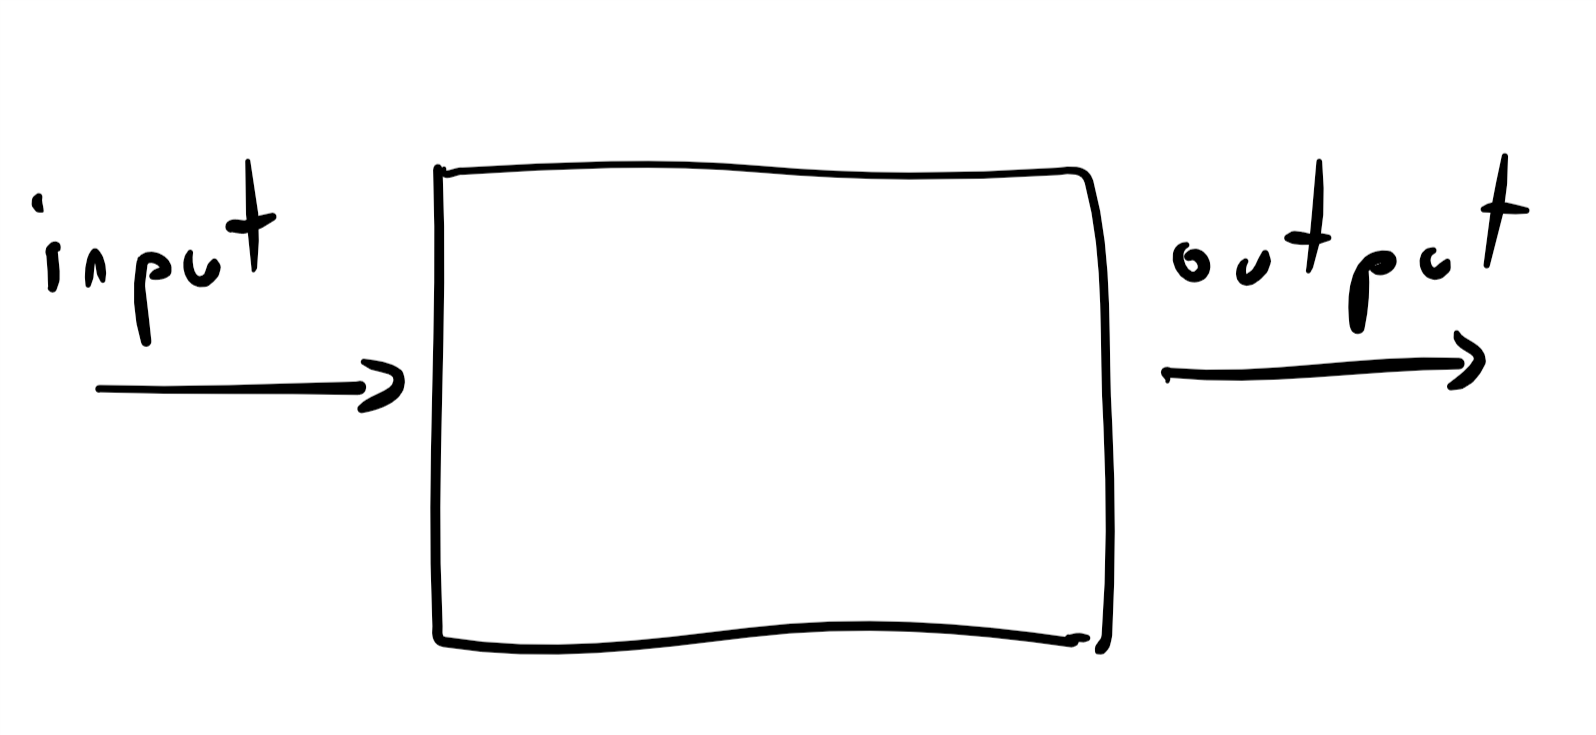
\includegraphics[width=\linewidth, height=1.5in, keepaspectratio]{../figure/input_output.png}
\caption{Our basic notion of \emph{computation} is some process that
maps an input to an output}
\label{computationinputtooutputfig}
\end{marginfigure}

When discussing computation, it is essential to separate the question of
\textbf{what} is the task we need to perform (i.e., the
\emph{specification}) from the question of \textbf{how} we achieve this
task (i.e., the \emph{implementation}). For example, as we've seen,
there is more than one way to achieve the computational task of
computing the product of two integers.

In this chapter we focus on the \textbf{what} part, namely defining
computational tasks. For starters, we need to define the inputs and
outputs. Capturing all the potential inputs and outputs that we might
ever want to compute on seems challenging, since computation today is
applied to a wide variety of objects. We do not compute merely on
numbers, but also on texts, images, videos, connection graphs of social
networks, MRI scans, gene data, and even other programs. We will
represent all these objects as \textbf{strings of zeroes and ones}, that
is objects such as \(0011101\) or \(1011\) or any other finite list of
\(1\)'s and \(0\)'s. (This choice is for convenience: there is nothing
``holy'' about zeroes and ones, and we could have used any other finite
collection of symbols.)


\begin{marginfigure}
\centering
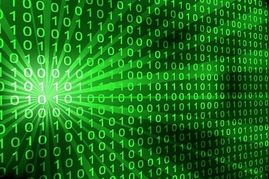
\includegraphics[width=\linewidth, height=1.5in, keepaspectratio]{../figure/zeroes-ones.jpg}
\caption{We represent numbers, texts, images, networks and many other
objects using strings of zeroes and ones. Writing the zeroes and ones
themselves in green font over a black background is optional.}
\label{zerosandonesgreenfig}
\end{marginfigure}

Today, we are so used to the notion of digital representation that we
are not surprised by the existence of such an encoding. But it is
actually a deep insight with significant implications. Many animals can
convey a particular fear or desire, but what is unique about humans is
\emph{language}: we use a finite collection of basic symbols to describe
a potentially unlimited range of experiences. Language allows
transmission of information over both time and space and enables
societies that span a great many people and accumulate a body of shared
knowledge over time.

Over the last several decades, we have seen a revolution in what we can
represent and convey in digital form. We can capture experiences with
almost perfect fidelity, and disseminate it essentially instantaneously
to an unlimited audience. Moreover, once information is in digital form,
we can \emph{compute} over it, and gain insights from data that were not
accessible in prior times. At the heart of this revolution is the simple
but profound observation that we can represent an unbounded variety of
objects using a finite set of symbols (and in fact using only the two
symbols \texttt{0} and \texttt{1}).

In later chapters, we will typically take such representations for
granted, and hence use expressions such as ``program \(P\) takes \(x\)
as input'' when \(x\) might be a number, a vector, a graph, or any other
object, when we really mean that \(P\) takes as input the
\emph{representation} of \(x\) as a binary string. However, in this
chapter we will dwell a bit more on how we can construct such
representations.

\section{Defining representations}\label{Defining-representations}

Every time we store numbers, images, sounds, databases, or other objects
on a computer, what we actually store in the computer's memory is the
\emph{representation} of these objects. Moreover, the idea of
representation is not restricted to digital computers. When we write
down text or make a drawing we are \emph{representing} ideas or
experiences as sequences of symbols (which might as well be strings of
zeroes and ones). Even our brain does not store the actual sensory
inputs we experience, but rather only a \emph{representation} of them.

To use objects such as numbers, images, graphs, or others as inputs for
computation, we need to define precisely how to represent these objects
as binary strings. A \emph{representation scheme} is a way to map an
object \(x\) to a binary string \(E(x) \in \{0,1\}^*\). For example, a
representation scheme for natural numbers is a function
\(E:\N \rightarrow \{0,1\}^*\). Of course, we cannot merely represent
all numbers as the string ``\(0011\)'' (for example). A minimal
requirement is that if two numbers \(x\) and \(x'\) are different then
they would be represented by different strings. Another way to say this
is that we require the encoding function \(E\) to be \emph{one to one}.

\subsection{Representing natural
numbers}\label{Representing-natural-numb}

We now show how we can represent natural numbers as binary strings. Over
the years people have represented numbers in a variety of ways,
including Roman numerals, tally marks, our own Hindu-Arabic decimal
system, and many others. We can use any one of those as well as many
others to represent a number as a string (see \cref{bitmapdigitsfig}).
However, for the sake of concreteness, we use the \emph{binary basis} as
our default representation of natural numbers as strings. For example,
we represent the number six as the string \(110\) since
\(1\cdot 2^{2} + 1 \cdot 2^1 + 0 \cdot 2^0 = 6\), and similarly we
represent the number thirty-five as the string \(y = 100011\) which
satisfies \(\sum_{i=0}^5 y_i \cdot 2^{|y|-i-1} = 35\). Some more
examples are given in the table below.


\begin{marginfigure}
\centering
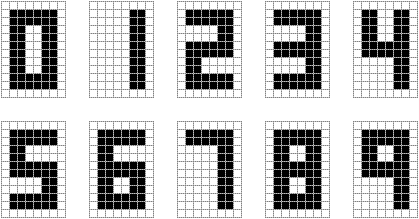
\includegraphics[width=\linewidth, height=1.5in, keepaspectratio]{../figure/digitsbitmap.png}
\caption{Representing each one the digits \(0,1,2,\ldots,9\) as a
\(12\times 8\) bitmap image, which can be thought of as a string in
\(\{0,1\}^{96}\). Using this scheme we can represent a natural number
\(x\) of \(n\) decimal digits as a string in \(\{0,1\}^{96n}\). Image
taken from
\href{http://blog.andersen.im/2010/12/autonomous-neural-development-and-pruning/}{blog
post of A. C. Andersen}.}
\label{bitmapdigitsfig}
\end{marginfigure}

\begin{longtable}[]{@{}ll@{}}
\caption{Representing numbers in the binary basis. The lefthand column
contains representations of natural numbers in the decimal basis, while
the righthand column contains representations of the same numbers in the
binary basis.}\tabularnewline
\toprule
\textbf{Number (decimal representation)} & \textbf{Number (binary
representation)}\tabularnewline
\midrule
\endfirsthead
\toprule
\textbf{Number (decimal representation)} & \textbf{Number (binary
representation)}\tabularnewline
\midrule
\endhead
0 & 0\tabularnewline
1 & 1\tabularnewline
2 & 10\tabularnewline
5 & 101\tabularnewline
16 & 10000\tabularnewline
40 & 101000\tabularnewline
53 & 110101\tabularnewline
389 & 110000101\tabularnewline
3750 & 111010100110\tabularnewline
\bottomrule
\end{longtable}

If \(n\) is even, then the least significant digit of \(n\)'s binary
representation is \(0\), while if \(n\) is odd then this digit equals
\(1\). Just like the number \(\floor{n/10}\) corresponds to ``chopping
off'' the least significant decimal digit (e.g.,
\(\floor{457/10}=\floor{45.7}=45\)), the number \(\floor{n/2}\)
corresponds to the ``chopping off'' the least significant \emph{binary}
digit. Hence the binary representation can be formally defined as the
following function \(NtS:\N \rightarrow \{0,1\}^*\) (\(NtS\) stands for
``natural numbers to strings''):

\[NtS(n) = \begin{cases}
            0    &  n=0 \\
            1    &  n=1 \\
            NtS(\floor{n/2}) parity(n) & n>1
\end{cases} \label{ntseq}\] where \(parity:\N \rightarrow \{0,1\}\) is
the function defined as \(parity(n)=0\) if \(n\) is even and
\(parity(n)=1\) if \(n\) is odd, and as usual, for strings
\(x,y \in \{0,1\}^*\), \(xy\) denotes the concatenation of \(x\) and
\(y\). The function \(NtS\) is defined \emph{recursively}: for every
\(n>0\) we define \(rep(n)\) in terms of the representation of the
smaller number \(\floor{n/2}\). It is also possible to define \(NtS\)
non-recursively, see \cref{binaryrepex}.

Throughout most of this book, the particular choices of representation
of numbers as binary strings would not matter much: we just need to know
that such a representation exists. In fact, for many of our purposes we
can even use the simpler representation of mapping a natural number
\(n\) to the length-\(n\) all-zero string \(0^n\).

\hypertarget{pythonbinary}{}
\begin{remark}[Binary representation in python (optional)] \label[remark]{pythonbinary}

We can implement the binary representation in \emph{Python} as follows:

\begin{code}
def NtS(n):# natural numbers to strings
    if n > 1:
        return NtS(n // 2) + str(n % 2)
    else:
        return str(n % 2)

print(NtS(236))
# 11101100

print(NtS(19))
# 10011
\end{code}

We can also use Python to implement the inverse transformation, mapping
a string back to the natural number it represents.

\begin{code}
def StN(x):# String to number
    k = len(x)-1
    return sum(int(x[i])*(2**(k-i)) for i in range(k+1))

print(StN(NtS(236)))
# 236
\end{code}

\end{remark}

\hypertarget{programmingrem}{}
\begin{remark}[Programming examples] \label[remark]{programmingrem}

In this book, we sometimes use \emph{code examples} as in
\cref{pythonbinary}. The point is always to emphasize that certain
computations can be achieved concretely, rather than illustrating the
features of Python or any other programming language. Indeed, one of the
messages of this book is that all programming languages are in a certain
precise sense \emph{equivalent} to one another, and hence we could have
just as well used JavaScript, C, COBOL, Visual Basic or even
\href{https://goo.gl/LKKNFK}{BrainF*ck}. This book is \emph{not} about
programming, and it is absolutely OK if you are not familiar with Python
or do not follow code examples such as those in \cref{pythonbinary}.

\end{remark}

\subsection{Meaning of representations
(discussion)}\label{Meaning-of-representation}

It is natural for us to think of \(236\) as the ``actual'' number, and
of \(11101100\) as ``merely'' its representation. However, for most
Europeans in the middle ages \texttt{CCXXXVI} would be the ``actual''
number and \(236\) (if they have even heard about it) would be the weird
Hindu-Arabic positional representation.\footnote{While the Babylonians
  already invented a positional system much earlier, the decimal
  positional system we use today was invented by Indian mathematicians
  around the third century. Arab mathematicians took it up in the 8th
  century. It first received significant attention in Europe with the
  publication of the 1202 book \emph{``Liber Abaci''} by Leonardo of
  Pisa, also known as Fibonacci, but it did not displace Roman numerals
  in common usage until the 15th century.} When our AI robot overlords
materialize, they will probably think of \(11101100\) as the ``actual''
number and of \(236\) as ``merely'' a representation that they need to
use when they give commands to humans.

So what is the ``actual'' number? This is a question that philosophers
of mathematics have pondered over throughout history. Plato argued that
mathematical objects exist in some ideal sphere of existence (that to a
certain extent is more ``real'' than the world we perceive via our
senses, as this latter world is merely the shadow of this ideal sphere).
In Plato's vision, the symbols \(236\) are merely notation for some
ideal object, that, in homage to the \href{https://goo.gl/b93h83}{late
musician}, we can refer to as ``the number commonly represented by
\(236\)''.

The Austrian philosopher Ludwig Wittgenstein, on the other hand, argued
that mathematical objects do not exist at all, and the only things that
exist are the actual marks on paper that make up \(236\), \(11101100\)
or \texttt{CCXXXVI}. In Wittgenstein's view, mathematics is merely about
formal manipulation of symbols that do not have any inherent meaning.
You can think of the ``actual'' number as (somewhat recursively) ``that
thing which is common to \(236\), \(11101100\) and \texttt{CCXXXVI} and
all other past and future representations that are meant to capture the
same object''.

While reading this book, you are free to choose your own philosophy of
mathematics, as long as you maintain the distinction between the
mathematical objects themselves and the various particular choices of
representing them, whether as splotches of ink, pixels on a screen,
zeroes and one, or any other form.

\section{Representations beyond natural
numbers}\label{Representations-beyond-na}

We have seen that natural numbers can be represented as binary strings.
We now show that the same is true for other types of objects, including
(potentially negative) integers, rational numbers, vectors, lists,
graphs and many others. In many instances, choosing the ``right'' string
representation for a piece of data is highly nontrivial, and finding the
``best'' one (e.g., most compact, best fidelity, most efficiently
manipulable, robust to errors, most informative features, etc.) is the
object of intense research. But for now, we focus on presenting some
simple representations for various objects that we would like to use as
inputs and outputs for computation.

\subsection{Representing (potentially negative)
integers}\label{repnegativeintegerssec}

Since we can represent natural numbers as strings, we can represent the
full set of \emph{integers} (i.e., members of the set
\(\Z=\{ \ldots, -3 , -2 , -1 , 0 , +1, +2, +3,\ldots \}\) ) by adding
one more bit that represents the sign. To represent a (potentially
negative) number \(m\), we prepend to the representation of the natural
number \(|m|\) a bit \(\sigma\) that equals \(0\) if \(m \geq 0\) and
equals \(1\) if \(m<0\). Formally, we define the function
\(ZtS:\Z \rightarrow \{0,1\}^*\) as follows \[ZtS(m) = \begin{cases}
0\;NtS(m) & m \geq 0  \\
1\;NtS(-m) & m < 0
\end{cases}\] where \(NtS\) is defined as in \eqref{ntseq}.

While the encoding function of a representation needs to be one to one,
it does not have to be \emph{onto}. For example, in the representation
above there is no number that is represented by the empty string but it
is still a fine representation, since every integer is represented
uniquely by some string.

\hypertarget{contextreprem}{}
\begin{remark}[Interpretation and context] \label[remark]{contextreprem}

Given a string \(y\in \{0,1\}^*\), how do we know if it's ``supposed''
to represent a (nonnegative) natural number or a (potentially negative)
integer? For that matter, even if we know \(y\) is ``supposed'' to be an
integer, how do we know what representation scheme it uses? The short
answer is that we do not necessarily know this information, unless it is
supplied from the context. (In programming languages, the compiler or
interpreter determines the representation of the sequence of bits
corresponding to a variable based on the variable's \emph{type}.) We can
treat the same string \(y\) as representing a natural number, an
integer, a piece of text, an image, or a green gremlin. Whenever we say
a sentence such as ``let \(n\) be the number represented by the string
\(y\),'' we will assume that we are fixing some canonical representation
scheme such as the ones above. The choice of the particular
representation scheme will rarely matter, except that we want to make
sure to stick with the same one for consistency.

\end{remark}

\subsection{Two's complement representation
(optional)}\label{twoscomplement}

\cref{repnegativeintegerssec}'s approach of representing an integer
using a specific ``sign bit'' is known as the \emph{Signed Magnitude
Representation} and was used in some early computers. However, the
\href{https://en.wikipedia.org/wiki/Two\%27s\%5Fcomplement}{two's
complement representation} is much more common in practice. The
\emph{two's complement representation} of an integer \(k\) in the set
\(\{ -2^n , -2^n+1, \ldots, 2^n-1 \}\) is the string \(ZtS_n(k)\) of
length \(n+1\) defined as follows: \[
ZtS_n(k) = \begin{cases} NtS_{n+1}(k) & 0 \leq k \leq 2^n-1 \\
                     NtS_{n+1}(2^{n+1}+k) & -2^n \leq k \leq -1 \end{cases} \;,
\] where \(NtS_\ell(m)\) demotes the standard binary representation of a
number \(m \in \{0,\ldots, 2^{\ell}\}\) as string of length \(\ell\),
padded with leading zeros as needed. For example, if \(n=3\) then
\(ZtS_3(1)=NtS_4(1)=0001\), \(ZtS_3(2)=NtS_4(2)=0010\),
\(ZtS_3(-1)=NtS_4(16-1)=1111\), and \(ZtS_3(-8)=NtS_4(16-8)=1000\). If
\(k\) is a negative number larger than or equal to \(-2^n\) then
\(2^{n+1}+k\) is a number between \(2^n\) and \(2^{n+1}-1\). Hence the
two's complement representation of such a number \(k\) is a string of
length \(n+1\) with its first digit equal to \(1\).

Another way to say this is that we represent a potentially negative
number \(k \in \{ -2^n,\ldots, 2^n-1 \}\) as the non-negative number
\(k \mod 2^{n+1}\) (see also \cref{twoscomplementfig}). This means that
if two (potentially negative) numbers \(k\) and \(k'\) are not too large
(i.e., \(|k|+|k'|<2^{n+1}\)), then we can compute the representation of
\(k+k'\) by adding modulo \(2^{n+1}\) the representations of \(k\) and
\(k'\) as if they were non-negative integers. This property of the two's
complement representation is its main attraction since, depending on
their architectures, microprocessors can often perform arithmetic
operations modulo \(2^w\) very efficiently (for certain values of \(w\)
such as \(32\) and \(64\)). Many systems leave it to the programmer to
check that values are not too large and will carry out this modular
arithmetic regardless of the size of the numbers involved. For this
reason, in some systems adding two large positive numbers can result in
a \emph{negative} number (e.g., adding \(2^n-100\) and \(2^n-200\) might
result in \(-300\) since \((2^{n+1}-300) \mod 2^{n+1} = -300\), see also
\cref{twoscomplementfig}).


\begin{marginfigure}
\centering
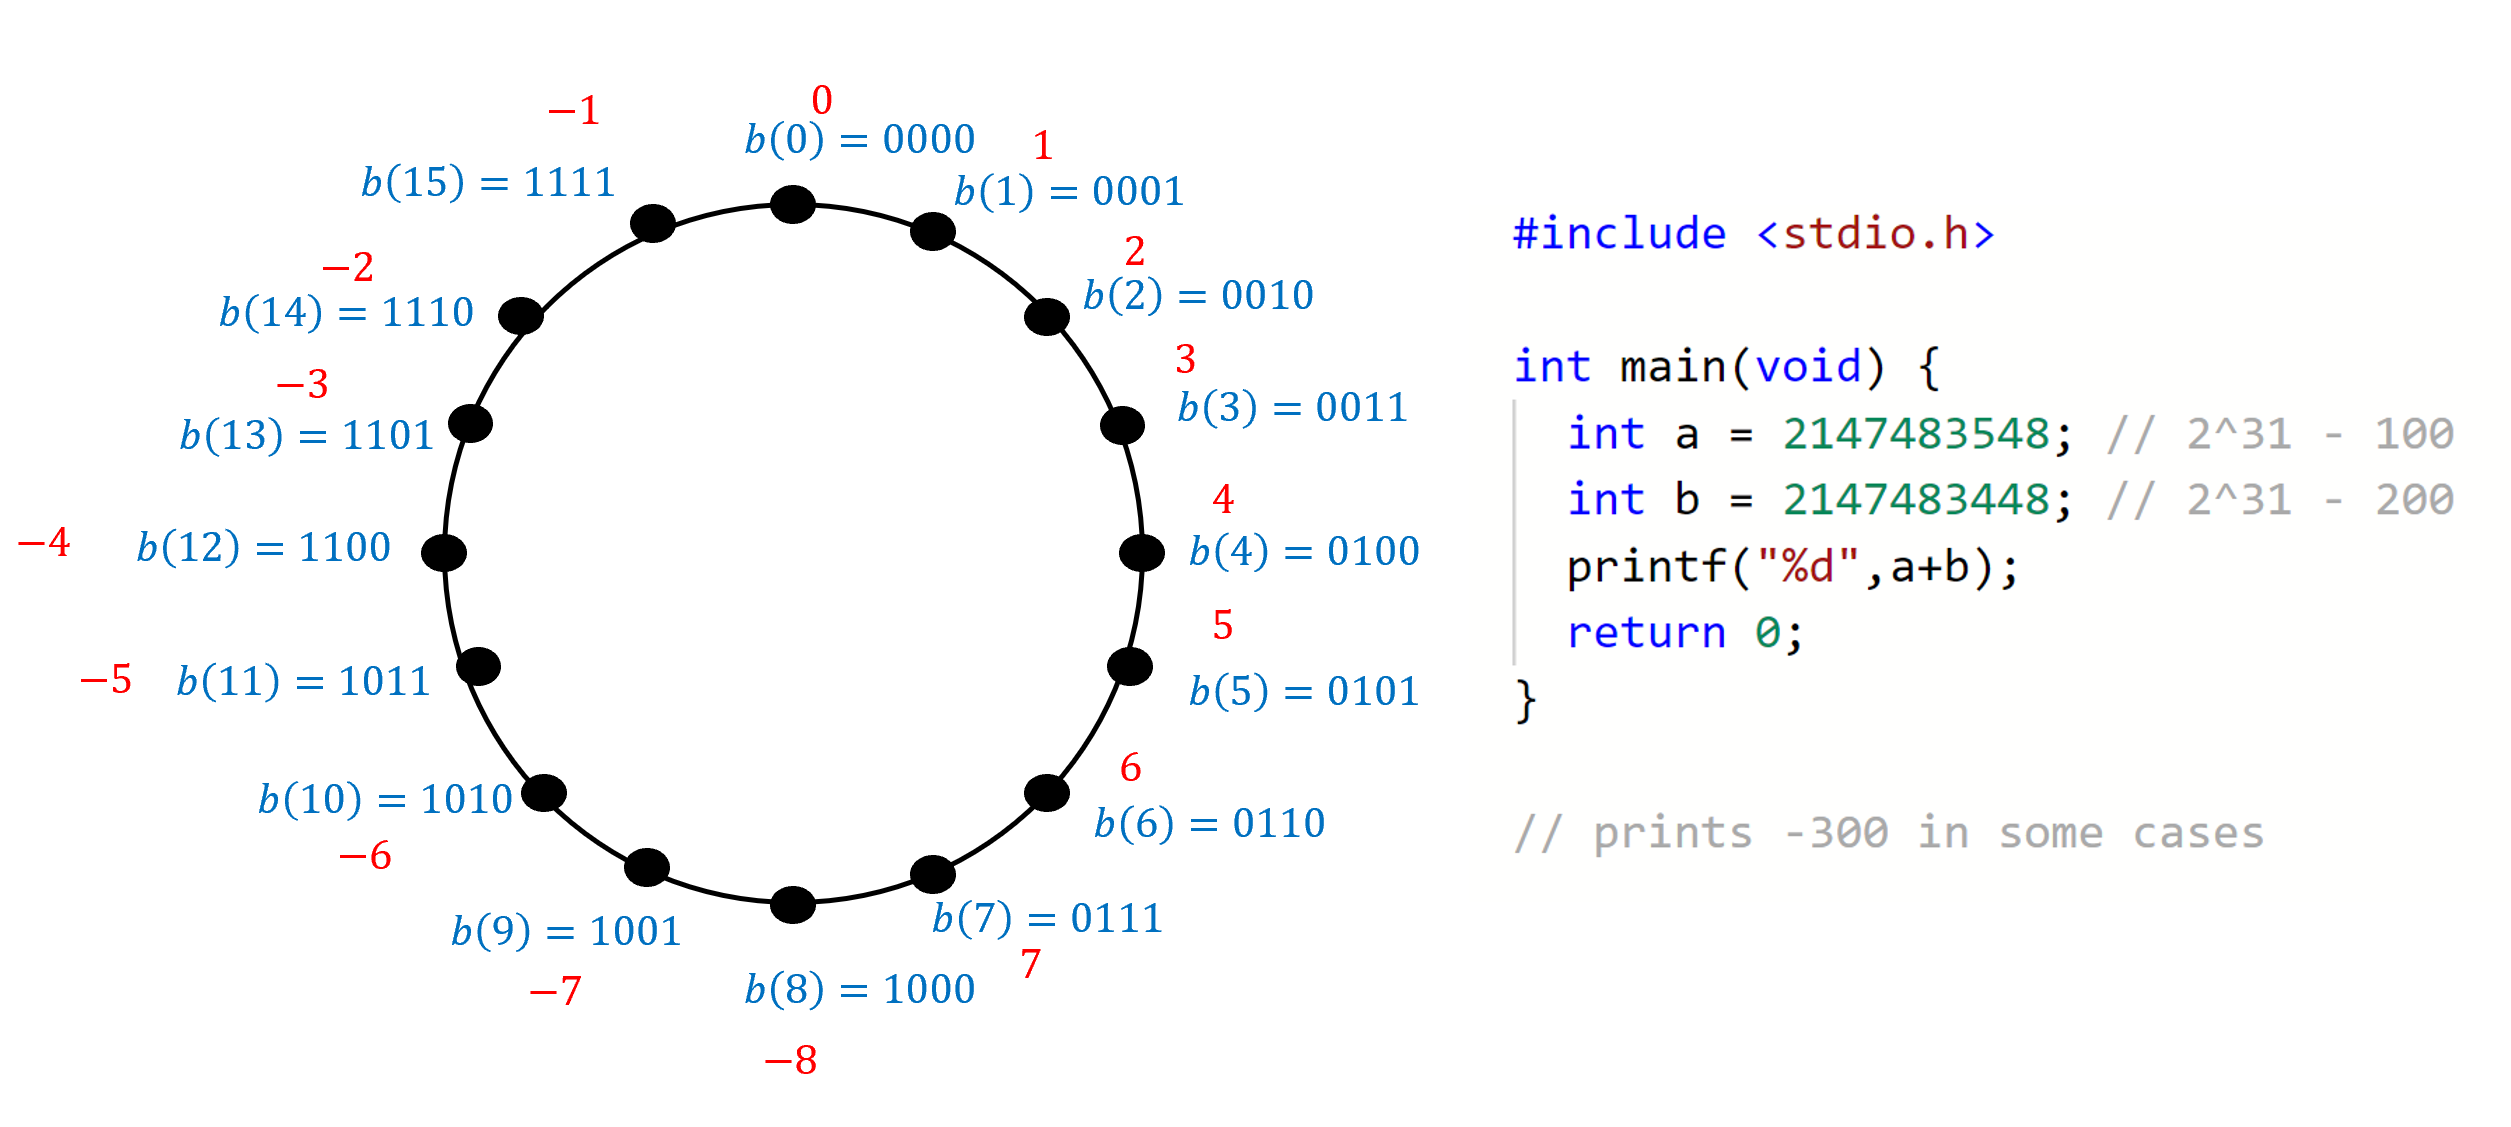
\includegraphics[width=\linewidth, height=1.5in, keepaspectratio]{../figure/twoscomplement.png}
\caption{In the \emph{two's complement representation} we represent a
potentially negative integer \(k \in \{ -2^n ,\ldots, 2^n-1 \}\) as an
\(n+1\) length string using the binary representation of the integer
\(k \mod 2^{n+1}\). On the lefthand side: this representation for
\(n=3\) (the red integers are the numbers being represented by the blue
binary strings). If a microprocessor does not check for overflows,
adding the two positive numbers \(6\) and \(5\) might result in the
negative number \(-5\) (since \(-5 \mod 16 = 11\). The righthand side is
a \texttt{C} program that will on some \(32\) bit architecture print a
negative number after adding two positive numbers. (Integer overflow in
\texttt{C} is considered \emph{undefined behavior} which means the
result of this program, including whether it runs or crashes, could
differ depending on the architecture, compiler, and even compiler
options and version.)}
\label{twoscomplementfig}
\end{marginfigure}

\subsection{Rational numbers, and representing pairs of
strings}\label{Rational-numbers-and-repr}

We can represent a rational number of the form \(a/b\) by representing
the two numbers \(a\) and \(b\). However, merely concatenating the
representations of \(a\) and \(b\) will not work. For example, the
binary representation of \(4\) is \(100\) and the binary representation
of \(43\) is \(101011\), but the concatenation \(100101011\) of these
strings is also the concatenation of the representation \(10010\) of
\(18\) and the representation \(1011\) of \(11\). Hence, if we used such
simple concatenation then we would not be able to tell if the string
\(100101011\) is supposed to represent \(4/43\) or \(18/11\).

We tackle this by giving a general representation for \emph{pairs of
strings}. If we were using a pen and paper, we would just use a
separator symbol such as \(\|\) to represent, for example, the pair
consisting of the numbers represented by \(10\) and \(110001\) as the
length-\(9\) string ``\(01\|110001\)''. In other words, there is a one
to one map \(F\) from \emph{pairs of strings} \(x,y \in \{0,1\}^*\) into
a single string \(z\) over the alphabet \(\Sigma = \{0,1,\| \}\) (in
other words, \(z\in \Sigma^*\)). Using such separators is similar to the
way we use spaces and punctuation to separate words in English. By
adding a little redundancy, we achieve the same effect in the digital
domain. We can map the three-element set \(\Sigma\) to the three-element
set \(\{00,11,01 \} \subset \{0,1\}^2\) in a one-to-one fashion, and
hence encode a length \(n\) string \(z\in \Sigma^*\) as a length \(2n\)
string \(w\in \{0,1\}^*\).

Our final representation for rational numbers is obtained by composing
the following steps:

\begin{enumerate}
\def\labelenumi{\arabic{enumi}.}
\item
  Representing a non-negative rational number as a pair of natural
  numbers.
\item
  Representing a natural number by a string via the binary
  representation.
\item
  Combining 1 and 2 to obtain a representation of a rational number as a
  pair of strings.
\item
  Representing a pair of strings over \(\{0,1\}\) as a single string
  over \(\Sigma = \{0,1,\|\}\).
\item
  Representing a string over \(\Sigma\) as a longer string over
  \(\{0,1\}\).
\end{enumerate}

\hypertarget{represnumberbypairs}{}
\begin{example}[Representing a rational number as a string] \label[example]{represnumberbypairs}

Consider the rational number \(r=-5/8\). We represent \(-5\) as \(1101\)
and \(+8\) as \(01000\), and so we can represent \(r\) as the
\emph{pair} of strings \((1101,01000)\) and represent this pair as the
length \(10\) string \(1101\|01000\) over the alphabet \(\{0,1,\|\}\).
Now, applying the map \(0 \mapsto 00\), \(1\mapsto 11\),
\(\| \mapsto 01\), we can represent the latter string as the length
\(20\) string \(s=11110011010011000000\) over the alphabet \(\{0,1\}\).

\end{example}

The same idea can be used to represent triples of strings, quadruples,
and so on as a string. Indeed, this is one instance of a very general
principle that we use time and again in both the theory and practice of
computer science (for example, in Object Oriented programming):

\hypertarget{representtuplesidea}{}
\begin{bigidea} \label[bigidea]{representtuplesidea}

If we can represent objects of type \(T\) as strings, then we can
represent tuples of objects of type \(T\) as strings as well.

\end{bigidea}

Repeating the same idea, once we can represent objects of type \(T\), we
can also represent \emph{lists of lists} of such objects, and even lists
of lists of lists and so on and so forth. We will come back to this
point when we discuss \emph{prefix free encoding} in
\cref{prefixfreesec}.

\section{Representing real numbers}\label{Representing-real-numbers}

The set of \emph{real numbers} \(\R\) contains all numbers including
positive, negative, and fractional, as well as \emph{irrational} numbers
such as \(\pi\) or \(e\). Every real number can be approximated by a
rational number, and thus we can represent every real number \(x\) by a
rational number \(a/b\) that is very close to \(x\). For example, we can
represent \(\pi\) by \(22/7\) within an error of about \(10^{-3}\). If
we want a smaller error (e.g., about \(10^{-4}\)) then we can use
\(311/99\), and so on and so forth.


\begin{figure}
\centering
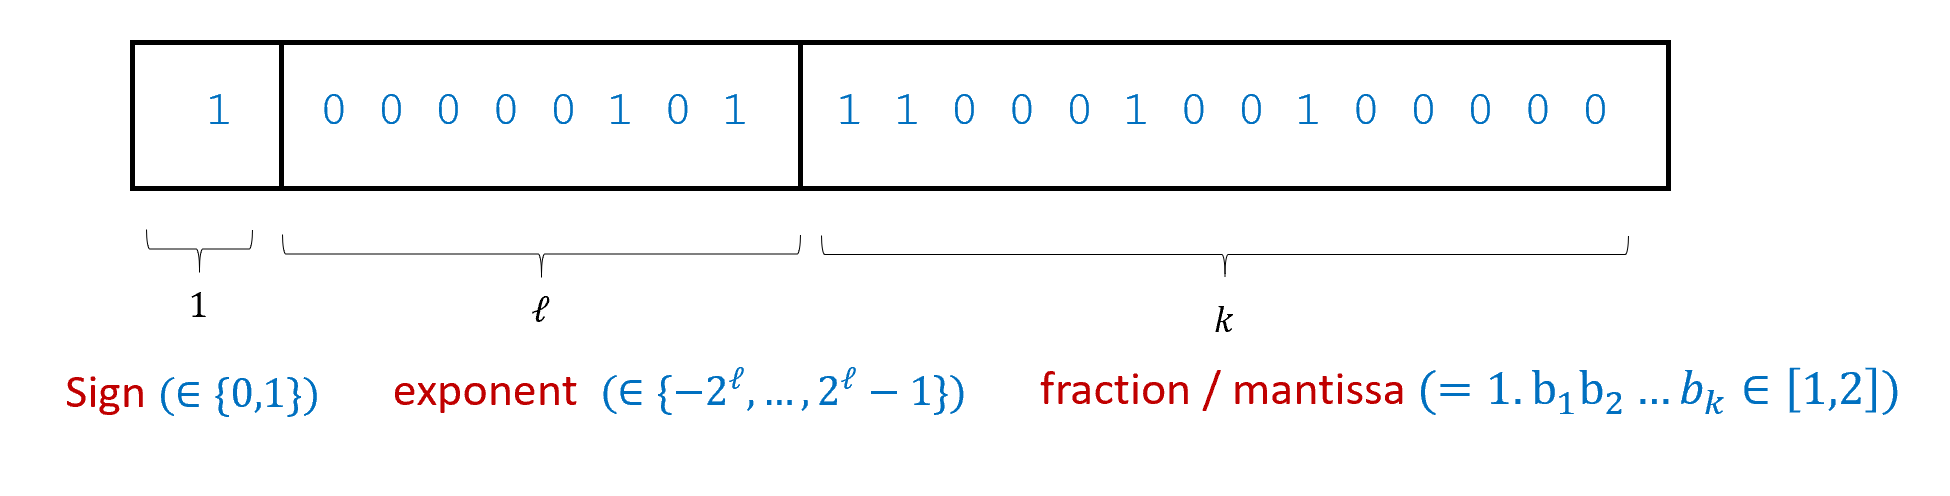
\includegraphics[width=\textwidth, height=0.25\paperheight, keepaspectratio]{../figure/floatingpoint.png}
\caption{The \emph{floating point representation} of a real number
\(x\in \R\) is its approximation as a number of the form
\(\sigma b \cdot 2^e\) where \(\sigma \in \{\pm 1 \}\), \(e\) is an
(potentially negative) integer, and \(b\) is a rational number between
\(1\) and \(2\) expressed as a binary fraction
\(1.b_0b_1b_2\ldots b_{k}\) for some \(b_1,\ldots,b_k \in \{0,1\}\)
(that is \(b = 1 + b_1/2 + b_2/4 + \ldots + b_k/2^k\)). Commonly-used
floating point representations fix the numbers \(\ell\) and \(k\) of
bits to represent \(e\) and \(b\) respectively. In the example above,
assuming we use two's complement representation for \(e\), the number
represented is
\(-1 \times 2^{5} \times ( 1 + 1/2 + 1/4 + 1/64 + 1/512) = -56.5625\).}
\label{floatingpointfig}
\end{figure}

The above representation of real numbers via rational numbers that
approximate them is a fine choice for a representation scheme. However,
typically in computing applications, it is more common to use the
\emph{floating point representation scheme} (see
\cref{floatingpointfig}) to represent real numbers. In the floating
point representation scheme we represent \(x\in \R\) by the pair
\((b,e)\) of (positive or negative) integers of some prescribed sizes
(determined by the desired accuracy) such that \(b \times 2^{e}\) is
closest to \(x\). Floating point representation is the base-two version
of \href{https://goo.gl/MUJnVE}{scientific notation}, where one
represents a number \(y\in R\) as its approximation of the form
\(b \times 10^e\) for \(b,e\). It is called ``floating point'' because
we can think of the number \(b\) as specifying a sequence of binary
digits, and \(e\) as describing the location of the ``binary point''
within this sequence. The use of floating representation is the reason
why in many programming systems, printing the expression
\texttt{0.1+0.2} will result in \texttt{0.30000000000000004} and not
\texttt{0.3}, see \href{http://floating-point-gui.de/}{here},
\href{https://docs.oracle.com/cd/E19957-01/806-3568/ncg_goldberg.html}{here}
and
\href{https://randomascii.wordpress.com/2012/04/05/floating-point-complexities/}{here}
for more.


\begin{marginfigure}
\centering
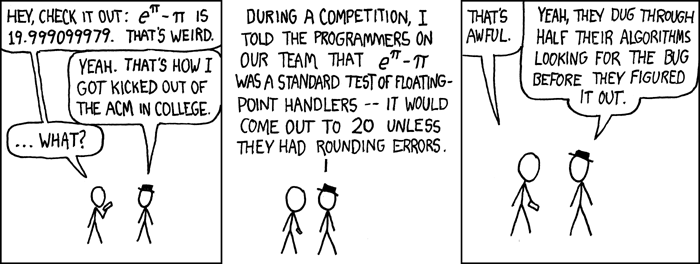
\includegraphics[width=\linewidth, height=1.5in, keepaspectratio]{../figure/e_to_the_pi_minus_pi.png}
\caption{XKCD cartoon on floating-point arithmetic.}
\label{xkcdfloatingfig}
\end{marginfigure}

The reader might be (rightly) worried about the fact that the floating
point representation (or the rational number one) can only
\emph{approximately} represent real numbers. In many (though not all)
computational applications, one can make the accuracy tight enough so
that this does not affect the final result, though sometimes we do need
to be careful. Indeed, floating-point bugs can sometimes be no joking
matter. For example, floating point rounding errors have been implicated
in the
\href{http://embeddedgurus.com/barr-code/2014/03/lethal-software-defects-patriot-missile-failure/}{failure}
of a U.S. Patriot missile to intercept an Iraqi Scud missile, costing 28
lives, as well as a 100 million pound error in computing
\href{https://catless.ncl.ac.uk/Risks/5/74}{payouts to British
pensioners}.

\subsection{Can we represent reals \emph{exactly}?}\label{cantorsec}

Given the issues with floating point approximations for real numbers, a
natural question is whether it is possible to represent real numbers
\emph{exactly} as strings. Unfortunately, the following theorem shows
that this cannot be done:

\hypertarget{cantorthm}{}
\begin{theorem}[Reals are uncountable] \label[theorem]{cantorthm}

There does not exist a one-to-one function
\(RtS:\R \rightarrow \{0,1\}^*\).\footnote{\(RtS\) stands for ``real
  numbers to strings''.}

\end{theorem}

\cref{cantorthm} was proven by
\href{https://en.wikipedia.org/wiki/Georg_Cantor}{Georg Cantor} in 1874.
(Cantor used the set \(\N\) rather than \(\{0,1\}^*\), but one can show
that these two results are equivalent using the one-to-one mappings
between those two sets, see \cref{naturalsstringsmapex}.) The
non-existence of such a map is equivalent to saying that there is no way
to ``count'' all the real numbers as some sequence
\(x_0,x_1,x_2,\ldots\). For this reason \cref{cantorthm} is known as the
\emph{uncountability of the reals}.

This result (and the theory around it) was quite shocking to
mathematicians at the time. By showing that there is no one-to-one map
from \(\R\) to \(\{0,1\}^*\) (or \(\N\)), Cantor showed that these two
infinite sets have ``different forms of infinity'' and that the set of
real numbers \(\R\) is in some sense ``bigger'' than the infinite set
\(\{0,1\}^*\). The notion that there are ``shades of infinity'' was
deeply disturbing to mathematicians and philosophers at the time. The
philosopher Ludwig Wittgenstein (whom we mentioned before) called
Cantor's results ``utter nonsense'' and ``laughable.'' Others thought
they were even worse than that. Leopold Kronecker called Cantor a
``corrupter of youth,'' while Henri Poincaré said that Cantor's ideas
``should be banished from mathematics once and for all.'' The tide
eventually turned, and these days Cantor's work is universally accepted
as the cornerstone of set theory and the foundations of mathematics. As
David Hilbert said in 1925, \emph{``No one shall expel us from the
paradise which Cantor has created for us.''} As we will see later in
this book, Cantor's ideas also play a huge role in the theory of
computation.

Now that we have discussed \cref{cantorthm}'s importance, let us see the
proof. It is achieved in two steps:

\begin{enumerate}
\def\labelenumi{\arabic{enumi}.}
\item
  Define some infinite set \(\mathcal{X}\) for which it is easier for us
  to prove that \(\mathcal{X}\) is not countable (namely, it's easier
  for us to prove that there is no one-to-one function from
  \(\mathcal{X}\) to \(\{0,1\}^*\)).
\item
  Prove that there \emph{is} a one-to-one function \(G\) mapping
  \(\mathcal{X}\) to \(\mathbb{R}\).
\end{enumerate}

We can use a proof by contradiction to show that these two facts
together imply \cref{cantorthm}. Specifically, if we assume (towards the
sake of contradiction) that there exists some one-to-one \(F\) mapping
\(\mathbb{R}\) to \(\{0,1\}^*\) then the function \(x \mapsto F(G(x))\)
obtained by composing \(F\) with the function \(G\) from Step 2 above
would be a one-to-one function from \(\mathcal{X}\) to \(\{0,1\}^*\),
which contradicts what we proved in Step 1!

To turn this idea into a full proof of \cref{cantorthm} we need to:

\begin{itemize}
\item
  Define the set \(\mathcal{X}\).
\item
  Prove that there is no one-to-one function from \(\mathcal{X}\) to
  \(\{0,1\}^*\)
\item
  Prove that there \emph{is} a one-to-one function from \(\mathcal{X}\)
  to \(\R\).
\end{itemize}

We now proceed to do precisely that. That is, we will define the set
\(\{0,1\}^\infty\), which will play the role of \(\mathcal{X}\), and
then state and prove two lemmas that show that this set satisfies our
two desired properties.

\hypertarget{bitsinfdef}{}
\begin{definition} \label[definition]{bitsinfdef}

We denote by \(\{0,1\}^\infty\) the set
\(\{ f \;|\; f:\N \rightarrow \{0,1\} \}\).

\end{definition}

That is, \(\{0,1\}^\infty\) is a set of \emph{functions}, and a function
\(f\) is in \(\{0,1\}^\infty\) iff its domain is \(\N\) and its codomain
is \(\{0,1\}\). We can also think of \(\{0,1\}^\infty\) as the set of
all infinite \emph{sequences} of bits, since a function
\(f:\N \rightarrow \{0,1\}\) can be identified with the sequence
\((f(0),f(1),f(2),\ldots )\). The following two lemmas show that
\(\{0,1\}^\infty\) can play the role of \(\mathcal{X}\) to establish
\cref{cantorthm}.

\hypertarget{sequencestostrings}{}
\begin{lemma} \label[lemma]{sequencestostrings}

There does not exist a one-to-one map
\(FtS:\{0,1\}^\infty \rightarrow \{0,1\}^*\).\footnote{\(FtS\) stands
  for ``functions to strings''.}

\end{lemma}

\hypertarget{sequencestoreals}{}
\begin{lemma} \label[lemma]{sequencestoreals}

There \emph{does} exist a one-to-one map
\(FtR:\{0,1\}^\infty \rightarrow \R\).\footnote{\(FtR\) stands for
  ``functions to reals.''}

\end{lemma}

As we've seen above, \cref{sequencestostrings} and
\cref{sequencestoreals} together imply \cref{cantorthm}. To repeat the
argument more formally, suppose, for the sake of contradiction, that
there did exist a one-to-one function \(RtS:\R \rightarrow \{0,1\}^*\).
By \cref{sequencestoreals}, there exists a one-to-one function
\(FtR:\{0,1\}^\infty \rightarrow \R\). Thus, under this assumption,
since the composition of two one-to-one functions is one-to-one (see
\cref{onetoonecompex}), the function
\(FtS:\{0,1\}^\infty \rightarrow \{0,1\}^*\) defined as
\(FtS(f)=RtS(FtR(f))\) will be one to one, contradicting
\cref{sequencestostrings}. See \cref{proofofcantorfig} for a graphical
illustration of this argument.


\begin{figure}
\centering
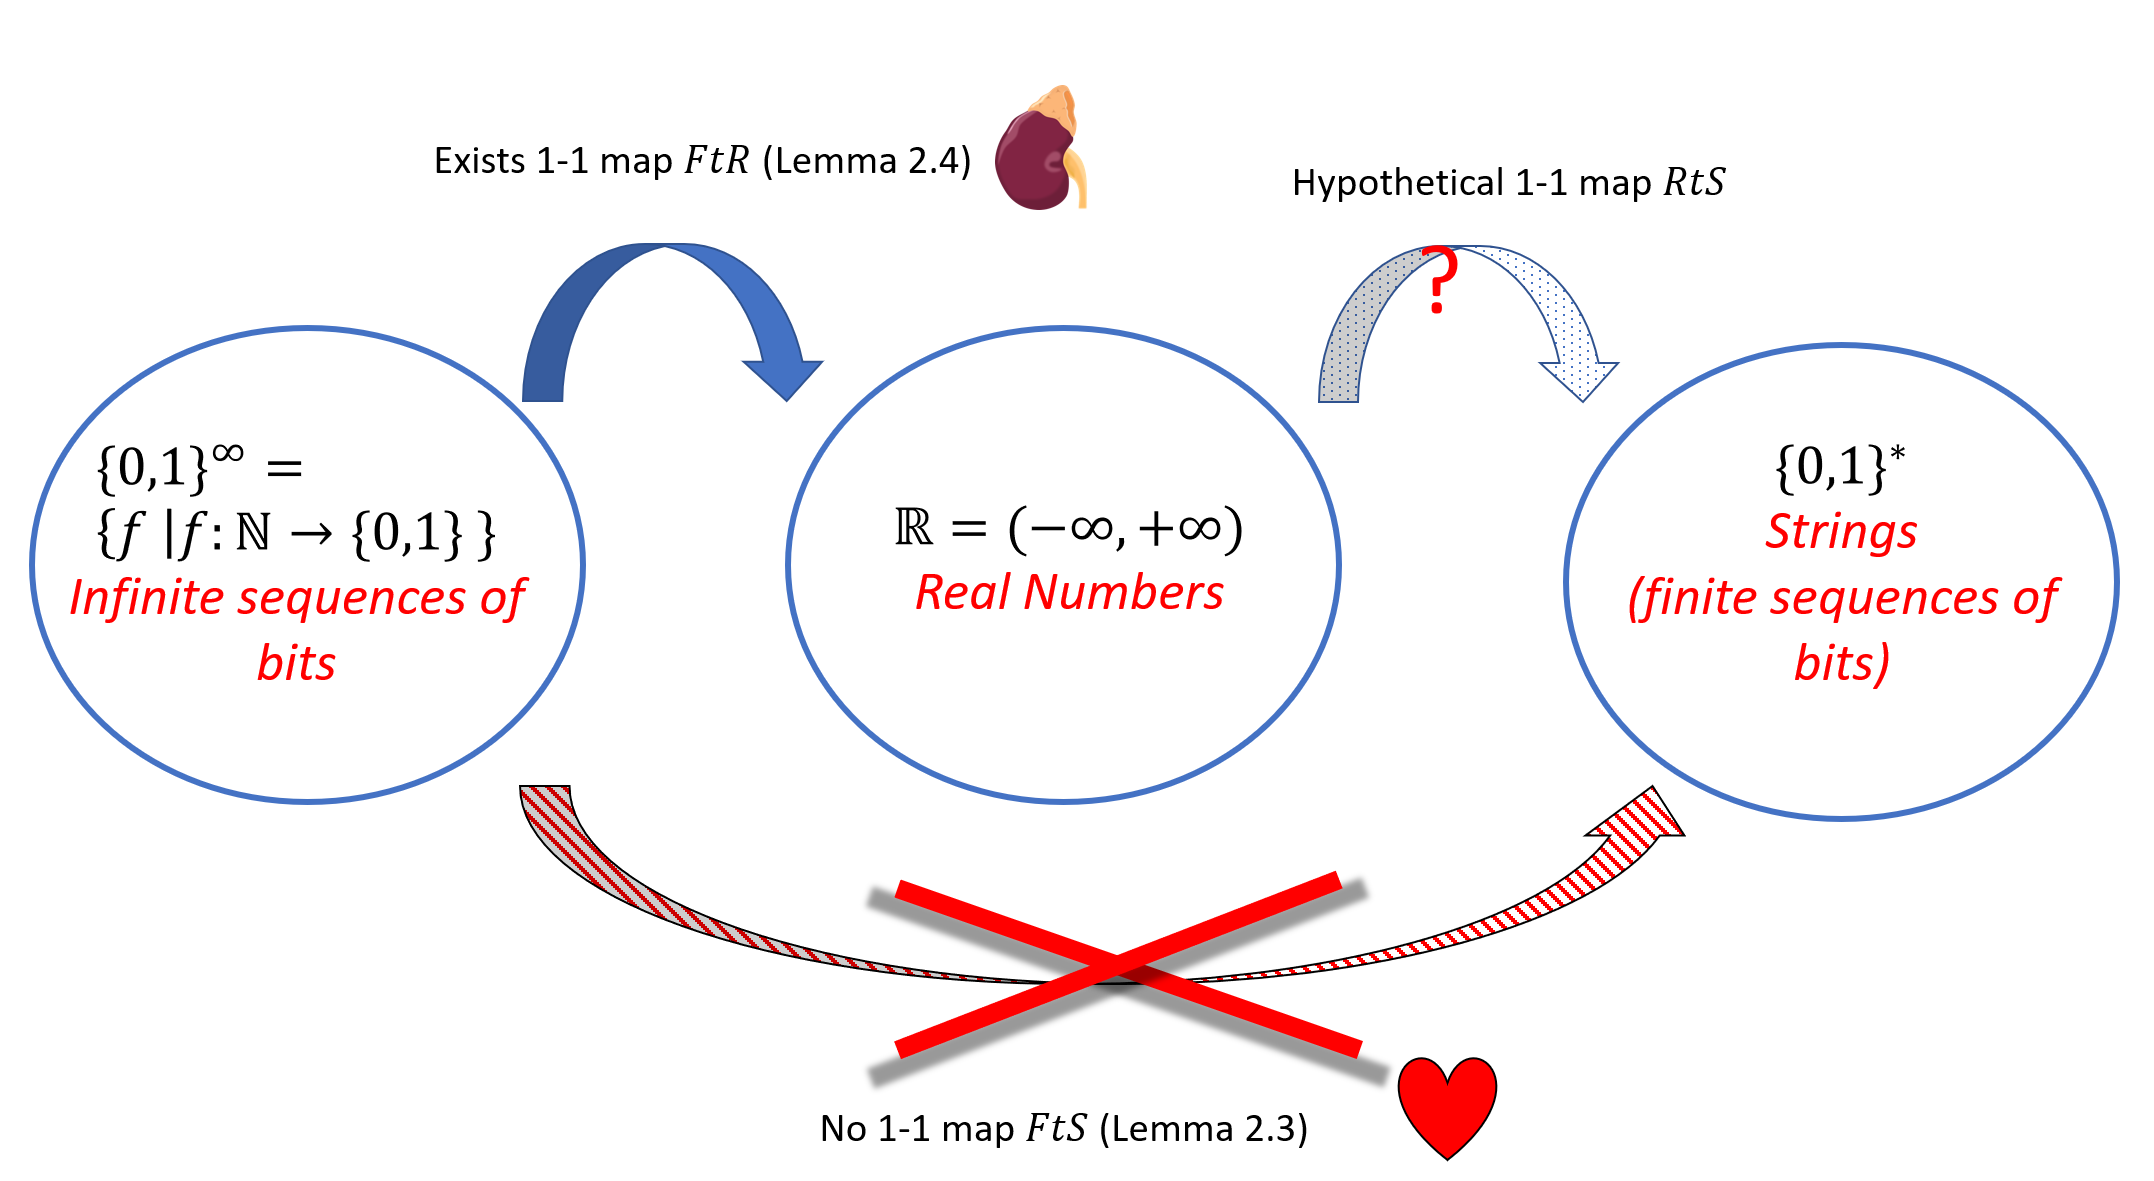
\includegraphics[width=\textwidth, height=0.25\paperheight, keepaspectratio]{../figure/proofofcantor.png}
\caption{We prove \cref{cantorthm} by combining
\cref{sequencestostrings} and \cref{sequencestoreals}.
\cref{sequencestoreals}, which uses standard calculus tools, shows the
existence of a one-to-one map \(FtR\) from the set \(\{0,1\}^\infty\) to
the real numbers. So, if a hypothetical one-to-one map
\(RtS:\R \rightarrow \{0,1\}^*\) existed, then we could compose them to
get a one-to-one map \(FtS:\{0,1\}^\infty \rightarrow \{0,1\}^*\). Yet
this contradicts \cref{sequencestostrings}- the heart of the proof-
which rules out the existence of such a map.}
\label{proofofcantorfig}
\end{figure}

Now all that is left is to prove these two lemmas. We start by proving
\cref{sequencestostrings} which is really the heart of \cref{cantorthm}.


\begin{figure}
\centering
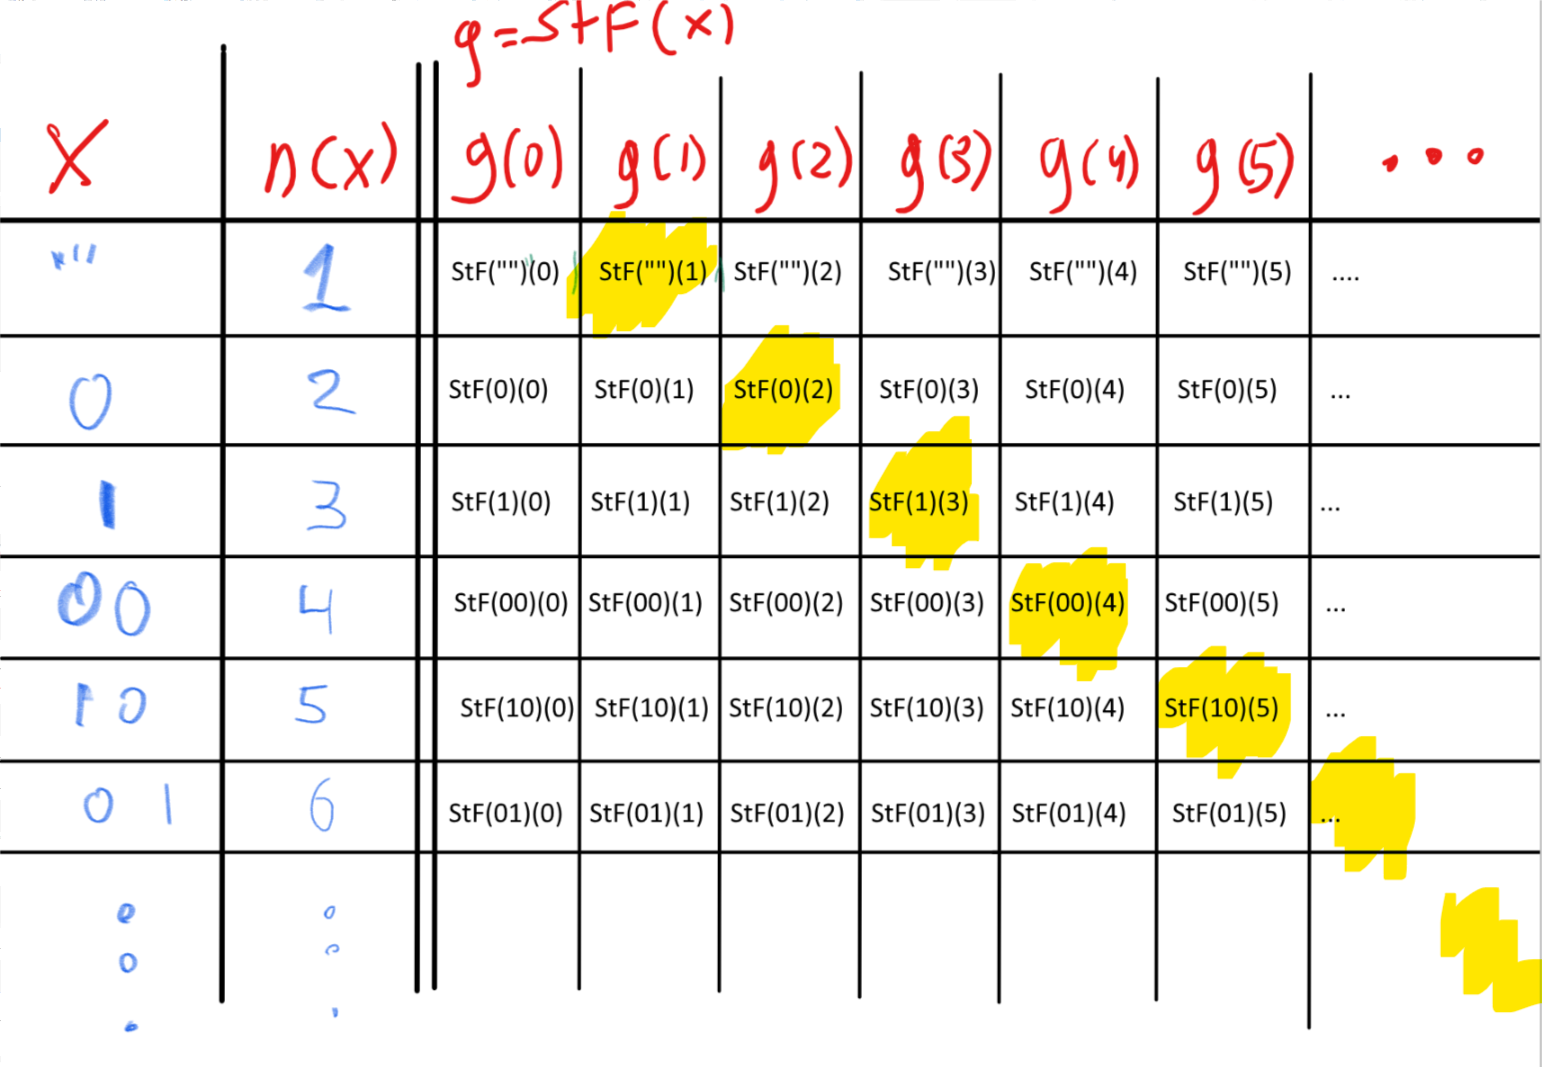
\includegraphics[width=\textwidth, height=0.25\paperheight, keepaspectratio]{../figure/diagreals2.png}
\caption{We construct a function \(\overline{d}\) such that
\(\overline{d} \neq StF(x)\) for every \(x\in \{0,1\}^*\) by ensuring
that \(\overline{d}(n(x)) \neq StF(x)(n(x))\) for every
\(x\in \{0,1\}^*\) with lexicographic order \(n(x)\). We can think of
this as building a table where the columns correspond to numbers
\(m\in \N\) and the rows correspond to \(x\in \{0,1\}^*\) (sorted
according to \(n(x)\)). If the entry in the \(x\)-th row and the
\(m\)-th column corresponds to \(g(m))\) where \(g=StF(x)\) then
\(\overline{d}\) is obtained by going over the ``diagonal'' elements in
this table (the entries corresponding to the \(x\)-th row and
\(n(x)\)-th column) and ensuring that
\(\overline{d}(x)(n(x)) \neq StF(x)(n(x))\).}
\label{diagrealsfig}
\end{figure}

\begin{proof}[Proof of \cref{sequencestostrings}] \label[proof]{We-will-prove-that-there-}

We will prove that there does not exist an \emph{onto} function
\(StF:\{0,1\}^* \rightarrow \{0,1\}^\infty\). This implies the lemma
since for every two sets \(A\) and \(B\), there exists an onto function
from \(A\) to \(B\) if and only if there exists a one-to-one function
from \(B\) to \(A\) (see \cref{onetooneimpliesonto}).

The technique of this proof is known as the ``diagonal argument'' and is
illustrated in \cref{diagrealsfig}. We assume, towards a contradiction,
that there exists such a function
\(StF:\{0,1\}^* \rightarrow \{0,1\}^\infty\). We will show that \(StF\)
is not onto by demonstrating a function
\(\overline{d}\in \{0,1\}^\infty\) such that
\(\overline{d} \neq StF(x)\) for every \(x\in \{0,1\}^*\). Consider the
lexicographic ordering of binary strings (i.e.,
\(\ensuremath{\text{\texttt{""}}}\),\(0\),\(1\),\(00\),\(01\),\(\ldots\)).
For every \(n\in \N\), we let \(x_n\) be the \(n\)-th string in this
order. That is \(x_0 =\ensuremath{\text{\texttt{""}}}\), \(x_1 = 0\),
\(x_2= 1\) and so on and so forth. We define the function
\(\overline{d} \in \{0,1\}^\infty\) as follows:
\[\overline{d}(n) = 1 - StF(x_n)(n)\] for every \(n\in \N\). That is, to
compute \(\overline{d}\) on input \(n\in\N\), we first compute
\(g= StF(x_n)\), where \(x_n \in \{0,1\}^*\) is the \(n\)-th string in
the lexicographical ordering. Since \(g \in \{0,1\}^\infty\), it is a
function mapping \(\N\) to \(\{0,1\}\). The value \(\overline{d}(n)\) is
defined to be the negation of \(g(n)\).

The definition of the function \(\overline{d}\) is a bit subtle. One way
to think about it is to imagine the function \(StF\) as being specified
by an infinitely long table, in which every row corresponds to a string
\(x\in \{0,1\}^*\) (with strings sorted in lexicographic order), and
contains the sequence \(StF(x)(0), StF(x)(1), StF(x)(2),\ldots\). The
\emph{diagonal} elements in this table are the values

\[StF(\ensuremath{\text{\texttt{""}}})(0),StF(0)(1),StF(1)(2),StF(00)(3), StF(01)(4),\ldots\]

which correspond to the elements \(StF(x_n)(n)\) in the \(n\)-th row and
\(n\)-th column of this table for \(n=0,1,2,\ldots\). The function
\(\overline{d}\) we defined above maps every \(n\in \N\) to the negation
of the \(n\)-th diagonal value.

To complete the proof that \(StF\) is not onto we need to show that
\(\overline{d} \neq StF(x)\) for every \(x\in \{0,1\}^*\). Indeed, let
\(x\in \{0,1\}^*\) be some string and let \(g = StF(x)\). If \(n\) is
the position of \(x\) in the lexicographical order then by construction
\(\overline{d}(n) = 1-g(n) \neq g(n)\) which means that
\(g \neq \overline{d}\) which is what we wanted to prove.

\end{proof}

\begin{pause} \label[pause]{The-proof-of-crefsequence}

The proof of \cref{sequencestostrings} is rather subtle, and worth
re-reading a second or third time. We will use the ``diagonal argument''
again several times later on in this book.

\end{pause}

\hypertarget{generalizepowerset}{}
\begin{remark}[Generalizing beyond strings and reals] \label[remark]{generalizepowerset}

\cref{sequencestostrings} doesn't really have much to do with the
natural numbers or the strings. An examination of the proof shows that
it really shows that for \emph{every} set \(S\), there is no one-to-one
map \(F:\{0,1\}^S \rightarrow S\) where \(\{0,1\}^S\) denotes the set
\(\{ f \;|\; f:S \rightarrow \{0,1\} \}\) of all Boolean functions with
domain \(S\). Since we can identify a subset \(V \subseteq S\) with its
characteristic function \(f=1_V\) (i.e., \(1_V(x)=1\) iff \(x\in V\)),
we can think of \(\{0,1\}^S\) also as the set of all \emph{subsets} of
\(S\). This subset is sometimes called the \emph{power set} of \(S\).

The proof of \cref{sequencestostrings} can be generalized to show that
there is no one-to-one map between a set and its power set. In
particular, it means that the set \(\{0,1\}^\R\) is ``even bigger'' than
\(\R\). Cantor used these ideas to construct an infinite hierarchy of
shades of infinity. The number of such shades turns out to be much
larger than \(|\N|\) or even \(|\R|\). He denoted the cardinality of
\(\N\) by \(\aleph_0\) and denoted the next largest infinite number by
\(\aleph_1\). (\(\aleph\) is the first letter in the Hebrew alphabet.)
Cantor also made the
\href{https://en.wikipedia.org/wiki/Continuum_hypothesis}{continuum
hypothesis} that \(|\R|=\aleph_1\). We will come back to the fascinating
story of this hypothesis later on in this book.
\href{https://www.scottaaronson.com/democritus/lec2.html}{This lecture
of Aaronson} mentions some of these issues (see also
\href{http://www.eecs70.org/static/notes/n10.pdf}{this Berkeley CS 70
lecture}).

\end{remark}

To complete the proof of \cref{cantorthm}, we need to show
\cref{sequencestoreals}. This requires some calculus background but is
otherwise straightforward. If you have not had much experience with
limits of a real series before, then the formal proof below might be a
little hard to follow. This part is not the core of Cantor's argument,
nor are such limits important to the remainder of this book, so you can
feel free to take \cref{sequencestoreals} on faith and skip the proof.

\begin{proofidea} \label[proofidea]{We-define-FtRf-to-be-the-}

We define \(FtR(f)\) to be the number between \(0\) and \(2\) whose
decimal expansion is \(f(0).f(1) f(2) \ldots\), or in other words
\(FtR(f) = \sum_{i=0}^{\infty} f(i) \cdot 10^{-i}\). To prove that
\(FtR\) is one to one, we need to show that if \(f \neq g\) then
\(FtR(f) \neq FtR(g)\). To do that we let \(k\in \N\) be the first input
on which \(f\) and \(g\) disagree. The numbers \(FtR(f)\) and \(FtR(g)\)
agree in the first \(k-1\) digits following the decimal point and
disagree in the \(k\)-th digit. One can then calculate and verify that
this means that \(|FtR(f)-FtR(g)| > 0.5 \cdot 10^{-k}\) which in
particular means that these two numbers are distinct from one another.
(You might wonder why we can't immediately deduce that two numbers that
differ in a digit are not the same. The issue is that we have to be a
little more careful when talking about infinite expansions. For example,
the number one half has two decimal expansions \(0.5\) and
\(0.49999\cdots\). However, this issue does not come up if (as in our
case) we restrict attention only to numbers with decimal expansions that
do not involve the digit \(9\).)

\end{proofidea}

\begin{proof}[Proof of \cref{sequencestoreals}] \label[proof]{For-every-f-in-infty-we-d}

For every \(f \in \{0,1\}^\infty\), we define \(FtR(f)\) to be the
number whose decimal expansion is \(f(0).f(1)f(2)f(3)\ldots\).

Formally we define \[
FtR(f) = \sum_{i=0}^\infty f(i) \cdot 10^{-i} \label{eqcantordecimalexpansion}
\] It is a known result in calculus (whose proof we will not repeat
here) that the series on the righthand side of
\eqref{eqcantordecimalexpansion} converges to a definite limit in
\(\mathbb{R}\).

We now prove that \(FtR\) is one to one. Let \(f,g\) be two distinct
functions in \(\{0,1\}^\infty\). Since \(f\) and \(g\) are distinct,
there must be some input on which they differ, and we define \(k\) to be
the smallest such input and assume without loss of generality that
\(f(k)=0\) and \(g(k)=1\). (Otherwise, if \(f(k)=1\) and \(g(k)=0\),
then we can simply switch the roles of \(f\) and \(g\).) The numbers
\(FtR(f)\) and \(FtR(g)\) agree with each other up to the \(k-1\)-th
digit up after the decimal point. Since this digit equals \(0\) for
\(FtR(f)\) and equals \(1\) for \(FtR(g)\), we claim that \(FtR(g)\) is
bigger than \(FtR(f)\) by at least \(0.5 \cdot 10^{-k}\). To see this
note that the difference \(FtR(g)-FtR(f)\) will be minimized if
\(g(\ell)=0\) for every \(\ell>k\) and \(f(\ell)=1\) for every
\(\ell>k\), in which case (since \(f\) and \(g\) agree up to the
\(k-1\)-th digit)

\[
FtR(g)-FtR(f) = 10^{-k} - 10^{-k-1} - 10^{-k-2} - 10^{-k-3} - \cdots \label{eqcantordecimalexpansion}
\]

Since the infinite series \(\sum_{j=0}^{\infty} 10^{-i}\) converges to
\(10/9\), it follows that for every such \(f\) and \(g\),
\(FtR(g) - FtR(f) \geq 10^{-k} - 10^{-k-1}\cdot (10/9) > 0\). In
particular we see that for every distinct \(f,g \in \{0,1\}^\infty\),
\(FtR(f) \neq FtR(g)\), implying that the function \(FtR\) is one to
one.

\end{proof}

\hypertarget{decimal}{}
\begin{remark}[Using decimal expansion (optional)] \label[remark]{decimal}

In the proof above we used the fact that \(1 + 1/10 + 1/100 + \cdots\)
converges to \(10/9\), which plugging into
\eqref{eqcantordecimalexpansion} yields that the difference between
\(FtR(g)\) and \(FtR(h)\) is at least
\(10^{-k} - 10^{-k-1}\cdot (10/9) > 0\). While the choice of the decimal
representation for \(FtR\) was arbitrary, we could not have used the
binary representation in its place. Had we used the \emph{binary}
expansion instead of decimal, the corresponding sequence
\(1 + 1/2 + 1/4 + \cdots\) converges to \(2/1=2\), and since
\(2^{-k} = 2^{-k-1} \cdot 2\), we could not have deduced that \(FtR\) is
one to one. Indeed there do exist pairs of distinct sequences
\(f,g\in \{0,1\}^\infty\) such that
\(\sum_{i=0}^\infty f(i)2^{-i} = \sum_{i=0}^\infty g(i)2^{-i}\). (For
example, the sequence \(1,0,0,0,\ldots\) and the sequence
\(0,1,1,1,\ldots\) have this property.)

\end{remark}

\section{Representing objects beyond
numbers}\label{Representing-objects-beyo}

Numbers are of course by no means the only objects that we can represent
as binary strings. A \emph{representation scheme} for representing
objects from some set \(\mathcal{O}\) consists of an \emph{encoding}
function that maps an object in \(\mathcal{O}\) to a string, and a
\emph{decoding} function that decodes a string back to an object in
\(\mathcal{O}\). Formally, we make the following definition:

\hypertarget{binaryrepdef}{}
\begin{definition}[String representation] \label[definition]{binaryrepdef}

Let \(\mathcal{O}\) be any set. A \emph{representation scheme} for
\(\mathcal{O}\) is a pair of functions \(E,D\) where
\(E:\mathcal{O} \rightarrow \{0,1\}^*\) is a total one-to-one function,
\(D:\{0,1\}^* \rightarrow_p \mathcal{O}\) is a (possibly partial)
function, and such that \(D\) and \(E\) satisfy that \(D(E(o))=o\) for
every \(o\in \mathcal{O}\). \(E\) is known as the \emph{encoding}
function and \(D\) is known as the \emph{decoding} function.

\end{definition}

Note that the condition \(D(E(o))=o\) for every \(o\in\mathcal{O}\)
implies that \(D\) is \emph{onto} (can you see why?). It turns out that
to construct a representation scheme we only need to find an
\emph{encoding} function. That is, every one-to-one encoding function
has a corresponding decoding function, as shown in the following lemma:

\hypertarget{decodelem}{}
\begin{lemma} \label[lemma]{decodelem}

Suppose that \(E: \mathcal{O} \rightarrow \{0,1\}^*\) is one-to-one.
Then there exists a function \(D:\{0,1\}^* \rightarrow \mathcal{O}\)
such that \(D(E(o))=o\) for every \(o\in \mathcal{O}\).

\end{lemma}

\begin{proof} \label[proof]{Let-o-be-some-arbitrary-e}

Let \(o_0\) be some arbitrary element of \(\mathcal{O}\). For every
\(x \in \{0,1\}^*\), there exists either zero or a single
\(o\in \mathcal{O}\) such that \(E(o)=x\) (otherwise \(E\) would not be
one-to-one). We will define \(D(x)\) to equal \(o_0\) in the first case
and this single object \(o\) in the second case. By definition
\(D(E(o))=o\) for every \(o\in \mathcal{O}\).

\end{proof}

\hypertarget{totaldecoding}{}
\begin{remark}[Total decoding functions] \label[remark]{totaldecoding}

While the decoding function of a representation scheme can in general be
a \emph{partial} function, the proof of \cref{decodelem} implies that
every representation scheme has a \emph{total} decoding function. This
observation can sometimes be useful.

\end{remark}

\subsection{Finite representations}\label{Finite-representations}

If \(\mathcal{O}\) is \emph{finite}, then we can represent every object
in \(\mathcal{O}\) as a string of length at most some number \(n\). What
is the value of \(n\)? Let us denote by \(\{0,1\}^{\leq n}\) the set
\(\{ x\in \{0,1\}^* : |x| \leq n \}\) of strings of length at most
\(n\). The size of \(\{0,1\}^{\leq n}\) is equal to \[
|\{0,1\}^0| + |\{0,1\}^1| + |\{0,1\}^2| + \cdots + |\{0,1\}^n| = \sum_{i=0}^n 2^i = 2^{n+1}-1
\] using the standard formula for summing a
\href{https://en.wikipedia.org/wiki/Geometric_progression}{geometric
progression}.

To obtain a representation of objects in \(\mathcal{O}\) as strings of
length at most \(n\) we need to come up with a one-to-one function from
\(\mathcal{O}\) to \(\{0,1\}^{\leq n}\). We can do so, if and only if
\(|\mathcal{O}| \leq 2^{n+1}-1\) as is implied by the following lemma:

\hypertarget{onetoone}{}
\begin{lemma} \label[lemma]{onetoone}

For every two finite sets \(S,T\), there exists a one-to-one
\(E:S \rightarrow T\) if and only if \(|S| \leq |T|\).

\end{lemma}

\begin{proof} \label[proof]{Let-kS-and-mT-and-so-writ}

Let \(k=|S|\) and \(m=|T|\) and so write the elements of \(S\) and \(T\)
as \(S = \{ s_0 , s_1, \ldots, s_{k-1} \}\) and
\(T= \{ t_0 , t_1, \ldots, t_{m-1} \}\). We need to show that there is a
one-to-one function \(E: S \rightarrow T\) iff \(k \leq m\). For the
``if'' direction, if \(k \leq m\) we can simply define \(E(s_i)=t_i\)
for every \(i\in [k]\). Clearly for \(i \neq j\),
\(t_i = E(s_i) \neq E(s_j) = t_j\), and hence this function is
one-to-one. In the other direction, suppose that \(k>m\) and
\(E: S \rightarrow T\) is some function. Then \(E\) cannot be
one-to-one. Indeed, for \(i=0,1,\ldots,m-1\) let us ``mark'' the element
\(t_j=E(s_i)\) in \(T\). If \(t_j\) was marked before, then we have
found two objects in \(S\) mapping to the same element \(t_j\).
Otherwise, since \(T\) has \(m\) elements, when we get to \(i=m-1\) we
mark all the objects in \(T\). Hence, in this case, \(E(s_m)\) must map
to an element that was already marked before. (This observation is
sometimes known as the ``Pigeon Hole Principle'': the principle that if
you have a pigeon coop with \(m\) holes, and \(k>m\) pigeons, then there
must be two pigeons in the same hole. )

\end{proof}

\subsection{Prefix-free encoding}\label{prefixfreesec}

When showing a representation scheme for rational numbers, we used the
``hack'' of encoding the alphabet \(\{ 0,1, \|\}\) to represent tuples
of strings as a single string. This is a special case of the general
paradigm of \emph{prefix-free} encoding. The idea is the following: if
our representation has the property that no string \(x\) representing an
object \(o\) is a \emph{prefix} (i.e., an initial substring) of a string
\(y\) representing a different object \(o'\), then we can represent a
\emph{list} of objects by merely concatenating the representations of
all the list members. For example, because in English every sentence
ends with a punctuation mark such as a period, exclamation, or question
mark, no sentence can be a prefix of another and so we can represent a
list of sentences by merely concatenating the sentences one after the
other. (English has some complications such as periods used for
abbreviations (e.g., ``e.g.'') or sentence quotes containing
punctuation, but the high level point of a prefix-free representation
for sentences still holds.)

It turns out that we can transform \emph{every} representation to a
prefix-free form. This justifies \cref{representtuplesidea}, and allows
us to transform a representation scheme for objects of a type \(T\) to a
representation scheme of \emph{lists} of objects of the type \(T\). By
repeating the same technique, we can also represent lists of lists of
objects of type \(T\), and so on and so forth. But first let us formally
define prefix-freeness:

\hypertarget{prefixfreedef}{}
\begin{definition}[Prefix free encoding] \label[definition]{prefixfreedef}

For two strings \(y,y'\), we say that \(y\) is a \emph{prefix} of \(y'\)
if \(|y| \leq |y'|\) and for every \(i<|y|\), \(y'_i = y_i\).

Let \(\mathcal{O}\) be a non-empty set and
\(E:\mathcal{O} \rightarrow \{0,1\}^*\) be a function. We say that \(E\)
is \emph{prefix-free} if \(E(o)\) is non-empty for every
\(o\in\mathcal{O}\) and there does not exist a distinct pair of objects
\(o, o' \in \mathcal{O}\) such that \(E(o)\) is a prefix of \(E(o')\).

\end{definition}

Recall that for every set \(\mathcal{O}\), the set \(\mathcal{O}^*\)
consists of all finite length tuples (i.e., \emph{lists}) of elements in
\(\mathcal{O}\). The following theorem shows that if \(E\) is a
prefix-free encoding of \(\mathcal{O}\) then by concatenating encodings
we can obtain a valid (i.e., one-to-one) representation of
\(\mathcal{O}^*\):

\hypertarget{prefixfreethm}{}
\begin{theorem}[Prefix-free implies tuple encoding] \label[theorem]{prefixfreethm}

Suppose that \(E:\mathcal{O} \rightarrow \{0,1\}^*\) is prefix-free.
Then the following map
\(\overline{E}:\mathcal{O}^* \rightarrow \{0,1\}^*\) is one to one, for
every \(o_0,\ldots,o_{k-1} \in \mathcal{O}^*\), we define \[
\overline{E}(o_0,\ldots,o_{k-1}) = E(o_0)E(o_1) \cdots E(o_{k-1}) \;.
\]

\end{theorem}

\begin{pause} \label[pause]{crefprefixfreethm-is-an-e}

\cref{prefixfreethm} is an example of a theorem that is a little hard to
parse, but in fact is fairly straightforward to prove once you
understand what it means. Therefore, I highly recommend that you pause
here to make sure you understand the statement of this theorem. You
should also try to prove it on your own before proceeding further.

\end{pause}


\begin{marginfigure}
\centering
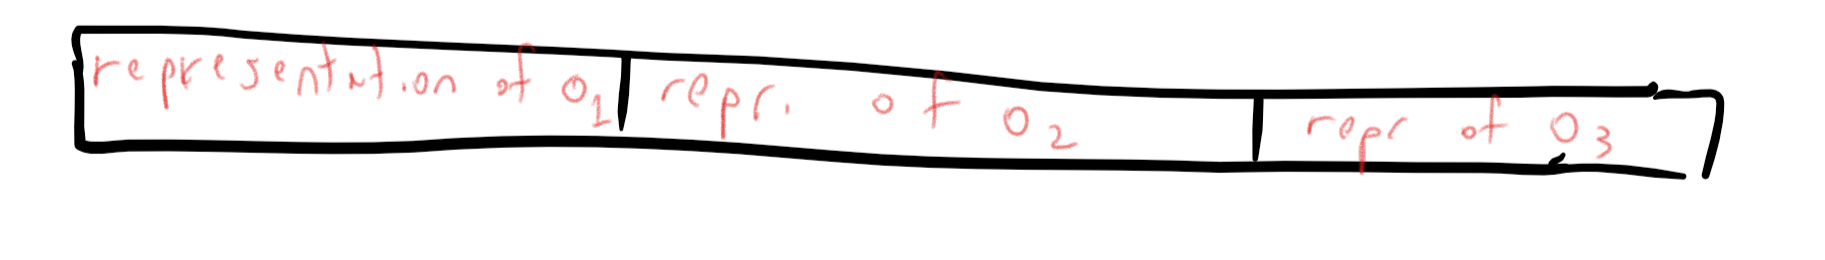
\includegraphics[width=\linewidth, height=1.5in, keepaspectratio]{../figure/repres_list.png}
\caption{If we have a prefix-free representation of each object then we
can concatenate the representations of \(k\) objects to obtain a
representation for the tuple \((o_0,\ldots,o_{k-1})\).}
\label{prefixfreerepconcat}
\end{marginfigure}

\begin{proofidea} \label[proofidea]{The-idea-behind-the-proof}

The idea behind the proof is simple. Suppose that for example we want to
decode a triple \((o_0,o_1,o_2)\) from its representation
\(x= \overline{E}(o_0,o_1,o_2)=E(o_0)E(o_1)E(o_2)\). We will do so by
first finding the first prefix \(x_0\) of \(x\) such is a representation
of some object. Then we will decode this object, remove \(x_0\) from
\(x\) to obtain a new string \(x'\), and continue onwards to find the
first prefix \(x_1\) of \(x'\) and so on and so forth (see
\cref{prefix-free-tuples-ex}). The prefix-freeness property of \(E\)
will ensure that \(x_0\) will in fact be \(E(o_0)\), \(x_1\) will be
\(E(o_1)\), etc.

\end{proofidea}

\begin{proof}[Proof of \cref{prefixfreethm}] \label[proof]{We-now-show-the-formal-pr}

We now show the formal proof. Suppose, towards the sake of
contradiction, that there exist two distinct tuples
\((o_0,\ldots,o_{k-1})\) and \((o'_0,\ldots,o'_{k'-1})\) such that

\[
\overline{E}(o_0,\ldots,o_{k-1})= \overline{E}(o'_0,\ldots,o'_{k'-1}) \;. \label{prefixfreeassump}
\] We will denote the string \(\overline{E}(o_0,\ldots,o_{k-1})\) by
\(\overline{x}\).

Let \(i\) be the first index such that \(o_i \neq o'_i\). (If
\(o_i=o'_i\) for all \(i\) then, since we assume the two tuples are
distinct, one of them must be larger than the other. In this case we
assume without loss of generality that \(k'>k\) and let \(i=k\).) In the
case that \(i<k\), we see that the string \(\overline{x}\) can be
written in two different ways:

\[
\overline{x} = \overline{E}(o_0,\ldots,o_{k-1}) = x_0\cdots x_{i-1} E(o_i) E(o_{i+1}) \cdots E(o_{k-1})
\]

and

\[
\overline{x} = \overline{E}(o'_0,\ldots,o'_{k'-1}) = x_0\cdots x_{i-1} E(o'_i) E(o'_{i+1}) \cdots E(o'_{k-1})
\]

where \(x_j = E(o_j) = E(o'_j)\) for all \(j<i\). Let \(\overline{y}\)
be the string obtained after removing the prefix \(x_0 \cdots x_{i-i}\)
from \(\overline{x}\). We see that \(\overline{y}\) can be written as
both \(\overline{y}= E(o_i)s\) for some string \(s\in \{0,1\}^*\) and as
\(\overline{y} = E(o'_i)s'\) for some \(s'\in \{0,1\}^*\). But this
means that one of \(E(o_i)\) and \(E(o'_i)\) must be a prefix of the
other, contradicting the prefix-freeness of \(E\).

In the case that \(i=k\) and \(k'>k\), we get a contradiction in the
following way. In this case

\[\overline{x} = E(o_0)\cdots E(o_{k-1}) = E(o_0) \cdots E(o_{k-1}) E(o'_k) \cdots E(o'_{k'-1})\]

which means that \(E(o'_k) \cdots E(o'_{k'-1})\) must correspond to the
empty string \(\text{\ensuremath{\text{\texttt{""}}}}\). But in such a
case \(E(o'_k)\) must be the empty string, which in particular is the
prefix of any other string, contradicting the prefix-freeness of \(E\).

\end{proof}

\hypertarget{prefixfreelistsrem}{}
\begin{remark}[Prefix freeness of list representation] \label[remark]{prefixfreelistsrem}

Even if the representation \(E\) of objects in \(\mathcal{O}\) is prefix
free, this does not mean that our representation \(\overline{E}\) of
\emph{lists} of such objects will be prefix free as well. In fact, it
won't be: for every three objects \(o,o',o''\) the representation of the
list \((o,o')\) will be a prefix of the representation of the list
\((o,o',o'')\). However, as we see in \cref{prefixfreetransformationlem}
below, we can transform \emph{every} representation into prefix-free
form, and so will be able to use that transformation if needed to
represent lists of lists, lists of lists of lists, and so on and so
forth.

\end{remark}

\subsection{Making representations
prefix-free}\label{Making-representations-pr}

Some natural representations are prefix-free. For example, every
\emph{fixed output length} representation (i.e., one-to-one function
\(E:\mathcal{O} \rightarrow \{0,1\}^n\)) is automatically prefix-free,
since a string \(x\) can only be a prefix of an equal-length \(x'\) if
\(x\) and \(x'\) are identical. Moreover, the approach we used for
representing rational numbers can be used to show the following:

\hypertarget{prefixfreetransformationlem}{}
\begin{lemma} \label[lemma]{prefixfreetransformationlem}

Let \(E:\mathcal{O} \rightarrow \{0,1\}^*\) be a one-to-one function.
Then there is a one-to-one prefix-free encoding \(\overline{E}\) such
that \(|\overline{E}(o)| \leq 2|E(o)|+2\) for every
\(o\in \mathcal{O}\).

\end{lemma}

\begin{pause} \label[pause]{For-the-sake-of-completen}

For the sake of completeness, we will include the proof below, but it is
a good idea for you to pause here and try to prove it on your own, using
the same technique we used for representing rational numbers.

\end{pause}

\begin{proof}[Proof of \cref{prefixfreetransformationlem}] \label[proof]{The-idea-behind-the-proof}

The idea behind the proof is to use the map \(0 \mapsto 00\),
\(1 \mapsto 11\) to ``double'' every bit in the string \(x\) and then
mark the end of the string by concatenating to it the pair \(01\). If we
encode a string \(x\) in this way, it ensures that the encoding of \(x\)
is never a prefix of the encoding of a distinct string \(x'\). Formally,
we define the function
\(\ensuremath{\mathit{PF}}:\{0,1\}^* \rightarrow \{0,1\}^*\) as follows:
\[\ensuremath{\mathit{PF}}(x)=x_0 x_0 x_1 x_1 \ldots x_{n-1}x_{n-1}01\]
for every \(x\in \{0,1\}^*\). If \(E:\mathcal{O} \rightarrow \{0,1\}^*\)
is the (potentially not prefix-free) representation for \(\mathcal{O}\),
then we transform it into a prefix-free representation
\(\overline{E}:\mathcal{O} \rightarrow \{0,1\}^*\) by defining
\(\overline{E}(o)=\ensuremath{\mathit{PF}}(E(o))\).

To prove the lemma we need to show that \textbf{(1)} \(\overline{E}\) is
one-to-one and \textbf{(2)} \(\overline{E}\) is prefix-free. In fact,
prefix freeness is a stronger condition than one-to-one (if two strings
are equal then in particular one of them is a prefix of the other) and
hence it suffices to prove \textbf{(2)}, which we now do.

Let \(o \neq o'\) in \(\mathcal{O}\) be two distinct objects. We will
prove that \(\overline{E}(o)\) is a not a prefix of
\(\overline{E}(o')\). Define \(x = E(o)\) and \(x'=E(o')\). Since \(E\)
is one-to-one, \(x \neq x'\). Under our assumption,
\(\ensuremath{\mathit{PF}}(x)\) is a prefix of
\(\ensuremath{\mathit{PF}}(x')\). If \(|x|<|x'|\) then the two bits in
positions \(2|x|,2|x|+1\) in \(\ensuremath{\mathit{PF}}(x)\) have the
value \(01\) but the corresponding bits in
\(\ensuremath{\mathit{PF}}(x')\) will equal either \(00\) or \(11\)
(depending on the \(|x|\)-th bit of \(x'\)) and hence
\(\ensuremath{\mathit{PF}}(x)\) cannot be a prefix of
\(\ensuremath{\mathit{PF}}(x')\). If \(|x|=|x'|\) then, since
\(x \neq x'\), there must be a coordinate \(i\) in which they differ,
meaning that the strings \(\ensuremath{\mathit{PF}}(x)\) and
\(\ensuremath{\mathit{PF}}(x')\) differ in the coordinates \(2i,2i+1\),
which again means that \(\ensuremath{\mathit{PF}}(x)\) cannot be a
prefix of \(\ensuremath{\mathit{PF}}(x')\). If \(|x|>|x'|\) then
\(|\ensuremath{\mathit{PF}}(x)|=2|x|+2>|\ensuremath{\mathit{PF}}(x')|=2|x'|+2\)
and hence \(\ensuremath{\mathit{PF}}(x)\) is longer than (and cannot be
a prefix of) \(\ensuremath{\mathit{PF}}(x')\). In all cases we see that
\(\ensuremath{\mathit{PF}}(x)=\overline{E}(o)\) is not a prefix of
\(\ensuremath{\mathit{PF}}(x')=\overline{E}(o')\), hence completing the
proof.

\end{proof}

The proof of \cref{prefixfreetransformationlem} is not the only or even
the best way to transform an arbitrary representation into prefix-free
form. \cref{prefix-free-ex} asks you to construct a more efficient
prefix-free transformation satisfying
\(|\overline{E}(o)| \leq |E(o)| + O(\log |E(o)|)\).

\subsection{``Proof by Python''
(optional)}\label{Proof-by-Python-optional}

The proofs of \cref{prefixfreethm} and
\cref{prefixfreetransformationlem} are \emph{constructive} in the sense
that they give us:

\begin{itemize}
\item
  A way to transform the encoding and decoding functions of any
  representation of an object \(O\) to encoding and decoding functions
  that are prefix-free, and
\item
  A way to extend prefix-free encoding and decoding of single objects to
  encoding and decoding of \emph{lists} of objects by concatenation.
\end{itemize}

Specifically, we could transform any pair of Python functions
\texttt{encode} and \texttt{decode} to functions \texttt{pfencode} and
\texttt{pfdecode} that correspond to a prefix-free encoding and
decoding. Similarly, given \texttt{pfencode} and \texttt{pfdecode} for
single objects, we can extend them to encoding of lists. Let us show how
this works for the case of the \texttt{NtS} and \texttt{StN} functions
we defined above.

We start with the ``Python proof'' of
\cref{prefixfreetransformationlem}: a way to transform an arbitrary
representation into one that is \emph{prefix free}. The function
\texttt{prefixfree} below takes as input a pair of encoding and decoding
functions, and returns a triple of functions containing
\emph{prefix-free} encoding and decoding functions, as well as a
function that checks whether a string is a valid encoding of an object.

\begin{code}
# takes functions encode and decode mapping
# objects to lists of bits and vice versa,
# and returns functions pfencode and pfdecode that
# maps objects to lists of bits and vice versa
# in a prefix-free way.
# Also returns a function pfvalid that says
# whether a list is a valid encoding
def prefixfree(encode, decode):
    def pfencode(o):
        L = encode(o)
        return [L[i//2] for i in range(2*len(L))]+[0,1]
    def pfdecode(L):
        return decode([L[j] for j in range(0,len(L)-2,2)])
    def pfvalid(L):
        return (len(L) % 2 == 0 ) and all(L[2*i]==L[2*i+1] for i in range((len(L)-2)//2)) and L[-2:]==[0,1]

    return pfencode, pfdecode, pfvalid

pfNtS, pfStN , pfvalidN = prefixfree(NtS,StN)

NtS(234)
# 11101010
pfNtS(234)
# 111111001100110001
pfStN(pfNtS(234))
# 234
pfvalidM(pfNtS(234))
# true
\end{code}

\begin{pause} \label[pause]{Note-that-the-Python-func}

Note that the Python function \texttt{prefixfree} above takes two
\emph{Python functions} as input and outputs three Python functions as
output. (When it's not too awkward, we use the term ``Python function''
or ``subroutine'' to distinguish between such snippets of Python
programs and mathematical functions.) You don't have to know Python in
this course, but you do need to get comfortable with the idea of
functions as mathematical objects in their own right, that can be used
as inputs and outputs of other functions.

\end{pause}

We now show a ``Python proof'' of \cref{prefixfreethm}. Namely, we show
a function \texttt{represlists} that takes as input a prefix-free
representation scheme (implemented via encoding, decoding, and validity
testing functions) and outputs a representation scheme for \emph{lists}
of such objects. If we want to make this representation prefix-free then
we could fit it into the function \texttt{prefixfree} above.

\begin{code}
def represlists(pfencode,pfdecode,pfvalid):
    """
    Takes functions pfencode, pfdecode and pfvalid,
    and returns functions encodelists, decodelists
    that can encode and decode lists of the objects
    respectively.
    """

    def encodelist(L):
        """Gets list of objects, encodes it as list of bits"""
        return "".join([pfencode(obj) for obj in L])

    def decodelist(S):
        """Gets lists of bits, returns lists of objects"""
        i=0; j=1 ; res = []
        while j<=len(S):
            if pfvalid(S[i:j]):
                res += [pfdecode(S[i:j])]
                i=j
            j+= 1
        return res

    return encodelist,decodelist


LtS , StL = represlists(pfNtS,pfStN,pfvalidN)

LtS([234,12,5])
# 111111001100110001111100000111001101
StL(LtS([234,12,5]))
# [234, 12, 5]
\end{code}

\subsection{Representing letters and
text}\label{Representing-letters-and-}

We can represent a letter or symbol by a string, and then if this
representation is prefix-free, we can represent a sequence of symbols by
merely concatenating the representation of each symbol. One such
representation is the \href{https://en.wikipedia.org/wiki/ASCII}{ASCII}
that represents \(128\) letters and symbols as strings of \(7\) bits.
Since the ASCII representation is fixed-length, it is automatically
prefix-free (can you see why?).
\href{https://en.wikipedia.org/wiki/Unicode}{Unicode} is representation
of (at the time of this writing) about 128,000 symbols as numbers (known
as \emph{code points}) between \(0\) and \(1,114,111\). There are
several types of prefix-free representations of the code points, a
popular one being \href{https://en.wikipedia.org/wiki/UTF-8}{UTF-8} that
encodes every codepoint into a string of length between \(8\) and
\(32\).


\begin{marginfigure}
\centering
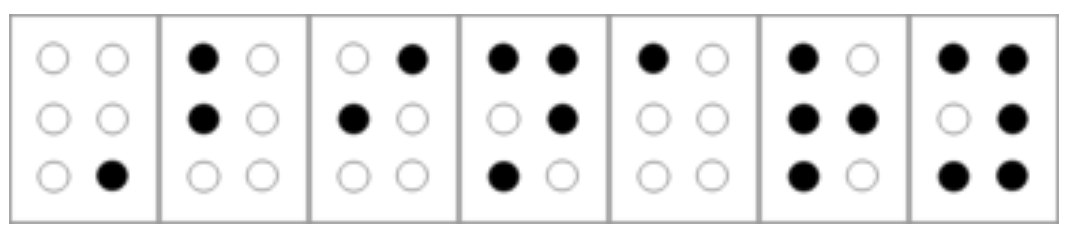
\includegraphics[width=\linewidth, height=1.5in, keepaspectratio]{../figure/braille.png}
\caption{The word ``Binary'' in ``Grade 1'' or ``uncontracted'' Unified
English Braille. This word is encoded using seven symbols since the
first one is a modifier indicating that the first letter is
capitalized.}
\label{braillefig}
\end{marginfigure}

\hypertarget{braille}{}
\begin{example}[The Braille representation] \label[example]{braille}

The \emph{Braille system} is another way to encode letters and other
symbols as binary strings. Specifically, in Braille, every letter is
encoded as a string in \(\{0,1\}^6\), which is written using indented
dots arranged in two columns and three rows, see \cref{braillefig}.
(Some symbols require more than one six-bit string to encode, and so
Braille uses a more general prefix-free encoding.)

The Braille system was invented in 1821 by
\href{https://goo.gl/Y2BkEe}{Louis Braille} when he was just 12 years
old (though he continued working on it and improving it throughout his
life). Braille was a French boy who lost his eyesight at the age of 5 as
the result of an accident.

\end{example}

\hypertarget{Crepresentation}{}
\begin{example}[Representing objects in C (optional)] \label[example]{Crepresentation}

We can use programming languages to probe how our computing environment
represents various values. This is easiest to do in ``unsafe''
programming languages such as \texttt{C} that allow direct access to the
memory.

Using a \href{https://goo.gl/L8oMzn}{simple \texttt{C} program} we have
produced the following representations of various values. One can see
that for integers, multiplying by 2 corresponds to a ``left shift''
inside each byte. In contrast, for floating point numbers, multiplying
by two corresponds to adding one to the exponent part of the
representation. In the architecture we used, a negative number is
represented using the \href{https://goo.gl/wov5fa}{two's complement}
approach. \texttt{C} represents strings in a prefix-free form by
ensuring that a zero byte is at their end.

\begin{code}
int      2    : 00000010 00000000 00000000 00000000
int      4    : 00000100 00000000 00000000 00000000
int      513  : 00000001 00000010 00000000 00000000
long     513  : 00000001 00000010 00000000 00000000 00000000 00000000 00000000 00000000
int      -1   : 11111111 11111111 11111111 11111111
int      -2   : 11111110 11111111 11111111 11111111
string   Hello: 01001000 01100101 01101100 01101100 01101111 00000000
string   abcd : 01100001 01100010 01100011 01100100 00000000
float    33.0 : 00000000 00000000 00000100 01000010
float    66.0 : 00000000 00000000 10000100 01000010
float    132.0: 00000000 00000000 00000100 01000011
double   132.0: 00000000 00000000 00000000 00000000 00000000 10000000 01100000 01000000
\end{code}

\end{example}

\subsection{Representing vectors, matrices,
images}\label{Representing-vectors-matr}

Once we can represent numbers and lists of numbers, then we can also
represent \emph{vectors} (which are just lists of numbers). Similarly,
we can represent lists of lists, and thus, in particular, can represent
\emph{matrices}. To represent an image, we can represent the color at
each pixel by a list of three numbers corresponding to the intensity of
Red, Green and Blue. (We can restrict to three primary colors since
\href{https://en.wikipedia.org/wiki/Tetrachromacy}{most} humans only
have three types of cones in their retinas; we would have needed 16
primary colors to represent colors visible to the
\href{https://goo.gl/t7JBfC}{Mantis Shrimp}.) Thus an image of \(n\)
pixels would be represented by a list of \(n\) such length-three lists.
A video can be represented as a list of images. Of course these
representations are rather wasteful and
\href{https://en.wikipedia.org/wiki/JPEG}{much}
\href{https://goo.gl/Vs8UhU}{more} compact representations are typically
used for images and videos, though this will not be our concern in this
book.

\subsection{Representing graphs}\label{Representing-graphs}

A \emph{graph} on \(n\) vertices can be represented as an \(n\times n\)
\emph{adjacency} matrix whose \((i,j)^{th}\) entry is equal to \(1\) if
the edge \((i,j)\) is present and is equal to \(0\) otherwise. That is,
we can represent an \(n\) vertex directed graph \(G=(V,E)\) as a string
\(A\in \{0,1\}^{n^2}\) such that \(A_{i,j}=1\) iff the edge
\(\overrightarrow{i\;j}\in E\). We can transform an undirected graph to
a directed graph by replacing every edge \(\{i,j\}\) with both edges
\(\overrightarrow{i\; j}\) and \(\overleftarrow{i\;j}\)

Another representation for graphs is the \emph{adjacency list}
representation. That is, we identify the vertex set \(V\) of a graph
with the set \([n]\) where \(n=|V|\), and represent the graph
\(G=(V,E)\) as a list of \(n\) lists, where the \(i\)-th list consists
of the out-neighbors of vertex \(i\). The difference between these
representations can be significant for some applications, though for us
would typically be immaterial.


\begin{marginfigure}
\centering
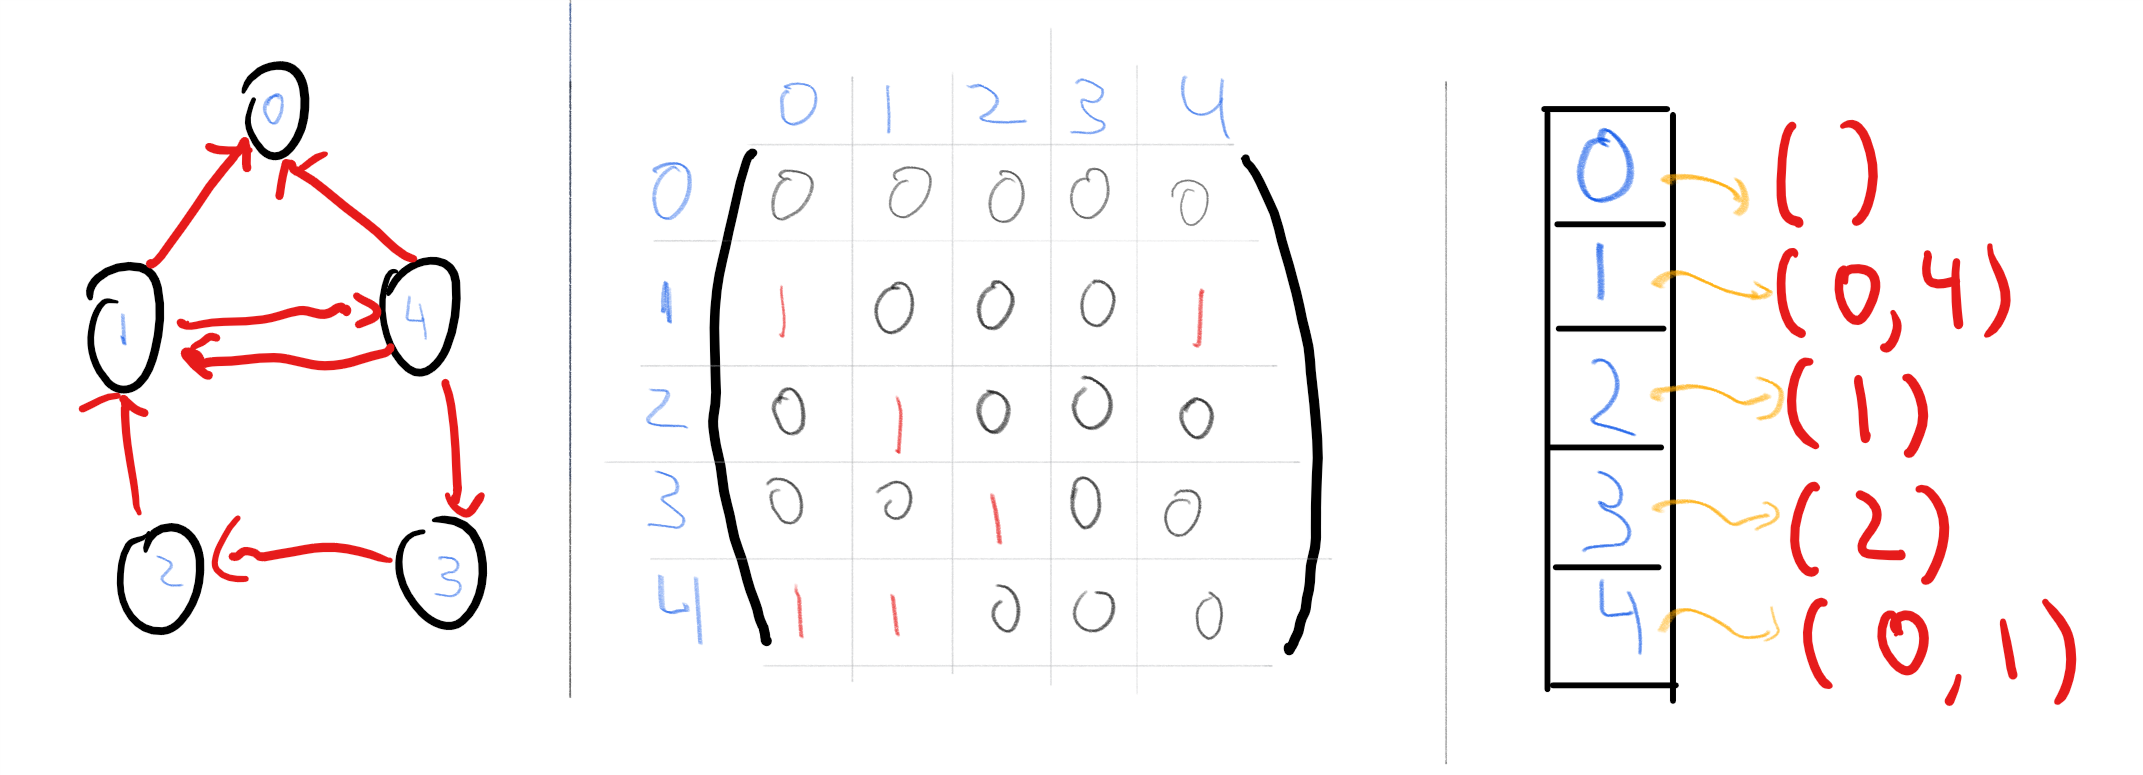
\includegraphics[width=\linewidth, height=1.5in, keepaspectratio]{../figure/representing_graphs.png}
\caption{Representing the graph
\(G=(\{0,1,2,3,4\},\{ (1,0),(4,0),(1,4),(4,1),(2,1),(3,2),(4,3) \})\) in
the adjacency matrix and adjacency list representations.}
\label{representinggraphsfig}
\end{marginfigure}

\subsection{Representing lists and nested
lists}\label{Representing-lists-and-ne}

If we have a way of representing objects from a set \(\mathcal{O}\) as
binary strings, then we can represent lists of these objects by applying
a prefix-free transformation. Moreover, we can use a trick similar to
the above to handle \emph{nested} lists. The idea is that if we have
some representation \(E:\mathcal{O} \rightarrow \{0,1\}^*\), then we can
represent nested lists of items from \(\mathcal{O}\) using strings over
the five element alphabet \(\Sigma = \{\)
\texttt{0},\texttt{1},\texttt{[} , \texttt{]} , \texttt{,} \(\}\). For
example, if \(o_1\) is represented by \texttt{0011}, \(o_2\) is
represented by \texttt{10011}, and \(o_3\) is represented by
\texttt{00111}, then we can represent the nested list
\((o_1,(o_2,o_3))\) as the string \texttt{"[0011,[10011,00111]]"} over
the alphabet \(\Sigma\). By encoding every element of \(\Sigma\) itself
as a three-bit string, we can transform any representation for objects
\(\mathcal{O}\) into a representation that enables representing
(potentially nested) lists of these objects.

\subsection{Notation}\label{Notation}

We will typically identify an object with its representation as a
string. For example, if \(F:\{0,1\}^* \rightarrow \{0,1\}^*\) is some
function that maps strings to strings and \(n\) is an integer, we might
make statements such as ``\(F(n)+1\) is prime'' to mean that if we
represent \(n\) as a string \(x\), then the integer \(m\) represented by
the string \(F(x)\) satisfies that \(m+1\) is prime. (You can see how
this convention of identifying objects with their representation can
save us a lot of cumbersome formalism.) Similarly, if \(x,y\) are some
objects and \(F\) is a function that takes strings as inputs, then by
\(F(x,y)\) we will mean the result of applying \(F\) to the
representation of the ordered pair \((x,y)\). We use the same notation
to invoke functions on \(k\)-tuples of objects for every \(k\).

This convention of identifying an object with its representation as a
string is one that we humans follow all the time. For example, when
people say a statement such as ``\(17\) is a prime number'', what they
really mean is that the integer whose decimal representation is the
string ``\texttt{17}'', is prime.

\begin{quote} \label[quote]{When-we-sayA-is-an-algori}

When we say

\emph{\(A\) is an algorithm that computes the multiplication function on
natural numbers.}

what we really mean is that

\emph{\(A\) is an algorithm that computes the function
\(F:\{0,1\}^* \rightarrow \{0,1\}^*\) such that for every pair
\(a,b \in \N\), if \(x\in \{0,1\}^*\) is a string representing the pair
\((a,b)\) then \(F(x)\) will be a string representing their product
\(a\cdot b\).}

\end{quote}

\section{Defining computational tasks as mathematical
functions}\label{Defining-computational-ta}

Abstractly, a \emph{computational process} is some process that takes an
input which is a string of bits and produces an output which is a string
of bits. This transformation of input to output can be done using a
modern computer, a person following instructions, the evolution of some
natural system, or any other means.

In future chapters, we will turn to mathematically defining
computational processes, but, as we discussed above, at the moment we
focus on \emph{computational tasks}. That is, we focus on the
\textbf{specification} and not the \textbf{implementation}. Again, at an
abstract level, a computational task can specify any relation that the
output needs to have with the input. However, for most of this book, we
will focus on the simplest and most common task of \emph{computing a
function}. Here are some examples:

\begin{itemize}
\item
  Given (a representation of) two integers \(x,y\), compute the product
  \(x\times y\). Using our representation above, this corresponds to
  computing a function from \(\{0,1\}^*\) to \(\{0,1\}^*\). We have seen
  that there is more than one way to solve this computational task, and
  in fact, we still do not know the best algorithm for this problem.
\item
  Given (a representation of) an integer \(z>1\), compute its
  \emph{factorization}; i.e., the list of primes
  \(p_1 \leq \cdots \leq p_k\) such that \(z = p_1\cdots p_k\). This
  again corresponds to computing a function from \(\{0,1\}^*\) to
  \(\{0,1\}^*\). The gaps in our knowledge of the complexity of this
  problem are even larger.
\item
  Given (a representation of) a graph \(G\) and two vertices \(s\) and
  \(t\), compute the length of the shortest path in \(G\) between \(s\)
  and \(t\), or do the same for the \emph{longest} path (with no
  repeated vertices) between \(s\) and \(t\). Both these tasks
  correspond to computing a function from \(\{0,1\}^*\) to
  \(\{0,1\}^*\), though it turns out that there is a vast difference in
  their computational difficulty.
\item
  Given the code of a Python program, determine whether there is an
  input that would force it into an infinite loop. This task corresponds
  to computing a \emph{partial} function from \(\{0,1\}^*\) to
  \(\{0,1\}\) since not every string corresponds to a syntactically
  valid Python program. We will see that we \emph{do} understand the
  computational status of this problem, but the answer is quite
  surprising.
\item
  Given (a representation of) an image \(I\), decide if \(I\) is a photo
  of a cat or a dog. This corresponds to computing some (partial)
  function from \(\{0,1\}^*\) to \(\{0,1\}\).
\end{itemize}

\hypertarget{booleanrem}{}
\begin{remark}[Boolean functions and languages] \label[remark]{booleanrem}

An important special case of computational tasks corresponds to
computing \emph{Boolean} functions, whose output is a single bit
\(\{0,1\}\). Computing such functions corresponds to answering a YES/NO
question, and hence this task is also known as a \emph{decision
problem}. Given any function \(F:\{0,1\}^* \rightarrow \{0,1\}\) and
\(x\in \{0,1\}^*\), the task of computing \(F(x)\) corresponds to the
task of deciding whether or not \(x\in L\) where
\(L = \{ x : F(x)=1 \}\) is known as the \emph{language} that
corresponds to the function \(F\). (The language terminology is due to
historical connections between the theory of computation and formal
linguistics as developed by Noam Chomsky.) Hence many texts refer to
such a computational task as \emph{deciding a language}.

\end{remark}


\begin{marginfigure}
\centering
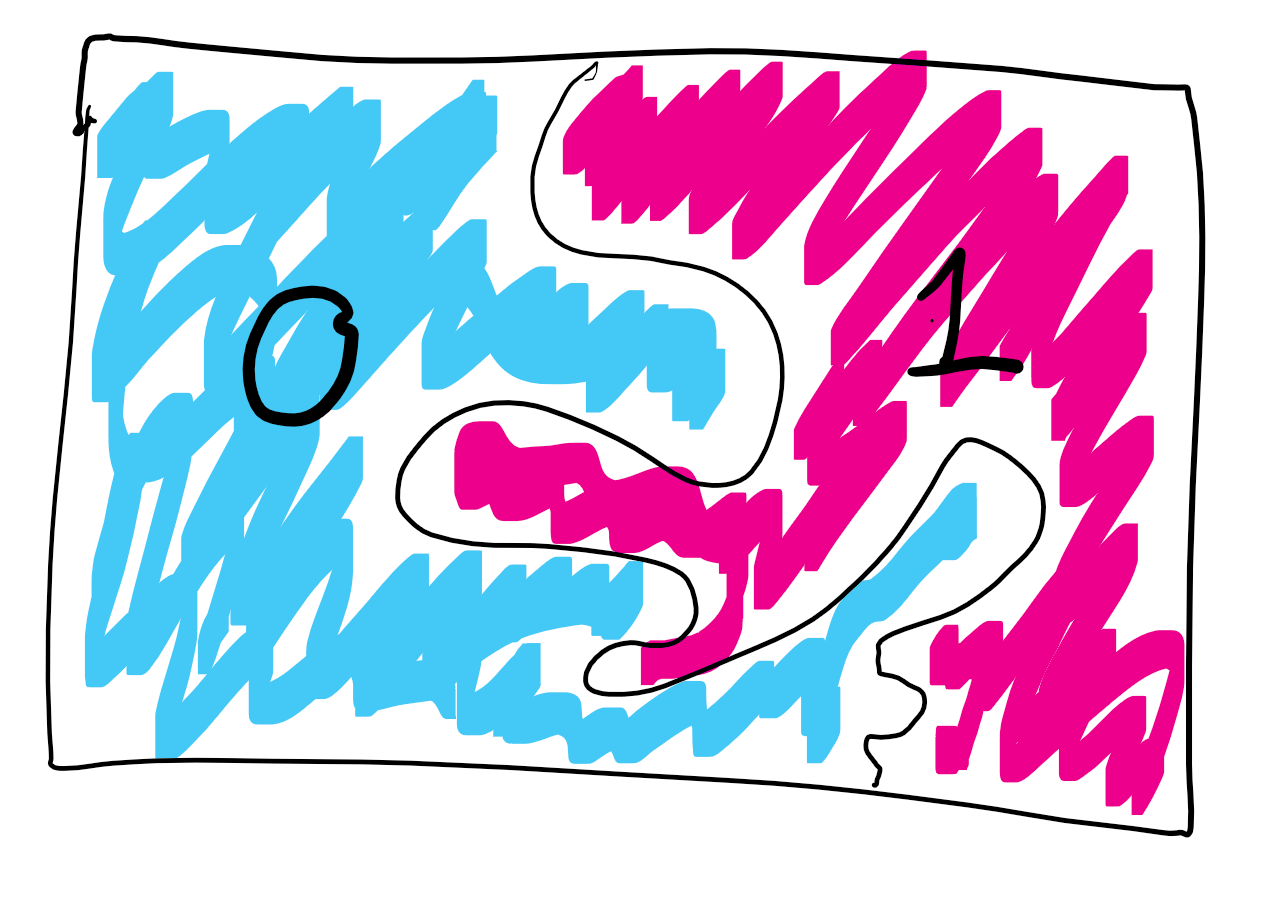
\includegraphics[width=\linewidth, height=1.5in, keepaspectratio]{../figure/booleanfunc.png}
\caption{A subset \(L \subseteq \{0,1\}^*\) can be identified with the
function \(F:\{0,1\}^* \rightarrow \{0,1\}\) such that \(F(x)=1\) if
\(x\in L\) and \(F(x)=0\) if \(x\not\in L\). Functions with a single bit
of output are called \emph{Boolean functions}, while subsets of strings
are called \emph{languages}. The above shows that the two are
essentially the same object, and we can identify the task of deciding
membership in \(L\) (known as \emph{deciding a language} in the
literature) with the task of computing the function \(F\).}
\label{booleanlangfig}
\end{marginfigure}

For every particular function \(F\), there can be several possible
\emph{algorithms} to compute \(F\). We will be interested in questions
such as:

\begin{itemize}
\item
  For a given function \(F\), can it be the case that \emph{there is no
  algorithm} to compute \(F\)?
\item
  If there is an algorithm, what is the best one? Could it be that \(F\)
  is ``effectively uncomputable'' in the sense that every algorithm for
  computing \(F\) requires a prohibitively large amount of resources?
\item
  If we cannot answer this question, can we show equivalence between
  different functions \(F\) and \(F'\) in the sense that either they are
  both easy (i.e., have fast algorithms) or they are both hard?
\item
  Can a function being hard to compute ever be a \emph{good thing}? Can
  we use it for applications in areas such as cryptography?
\end{itemize}

In order to do that, we will need to mathematically define the notion of
an \emph{algorithm}, which is what we will do in \cref{compchap}.

\subsection{Distinguish functions from programs!}\label{secimplvsspec}

You should always watch out for potential confusions between
\textbf{specifications} and \textbf{implementations} or equivalently
between \textbf{mathematical functions} and
\textbf{algorithms/programs}. It does not help that programming
languages (Python included) use the term \emph{``functions''} to denote
(parts of) \emph{programs}. This confusion also stems from thousands of
years of mathematical history, where people typically defined functions
by means of a way to compute them.

For example, consider the multiplication function on natural numbers.
This is the function
\(\ensuremath{\mathit{MULT}}:\N\times \N \rightarrow \N\) that maps a
pair \((x,y)\) of natural numbers to the number \(x \cdot y\). As we
mentioned, it can be implemented in more than one way:

\begin{code}
def mult1(x,y):
    res = 0
    while y>0:
        res += x
        y   -= 1
    return res

def mult2(x,y):
    a = str(x) # represent x as string in decimal notation
    b = str(y) # represent y as string in decimal notation
    res = 0
    for i in range(len(a)):
        for j in range(len(b)):
            res += int(a[len(a)-i])*int(b[len(b)-j])*(10**(i+j))
    return res

print(mult1(12,7))
# 84
print(mult2(12,7))
# 84
\end{code}

Both \texttt{mult1} and \texttt{mult2} produce the same output given the
same pair of natural number inputs. (Though \texttt{mult1} will take far
longer to do so when the numbers become large.) Hence, even though these
are two different \emph{programs}, they compute the same
\emph{mathematical function}. This distinction between a \emph{program}
or \emph{algorithm} \(A\), and the \emph{function} \(F\) that \(A\)
\emph{computes} will be absolutely crucial for us in this course (see
also \cref{functionornotfig}).


\begin{marginfigure}
\centering
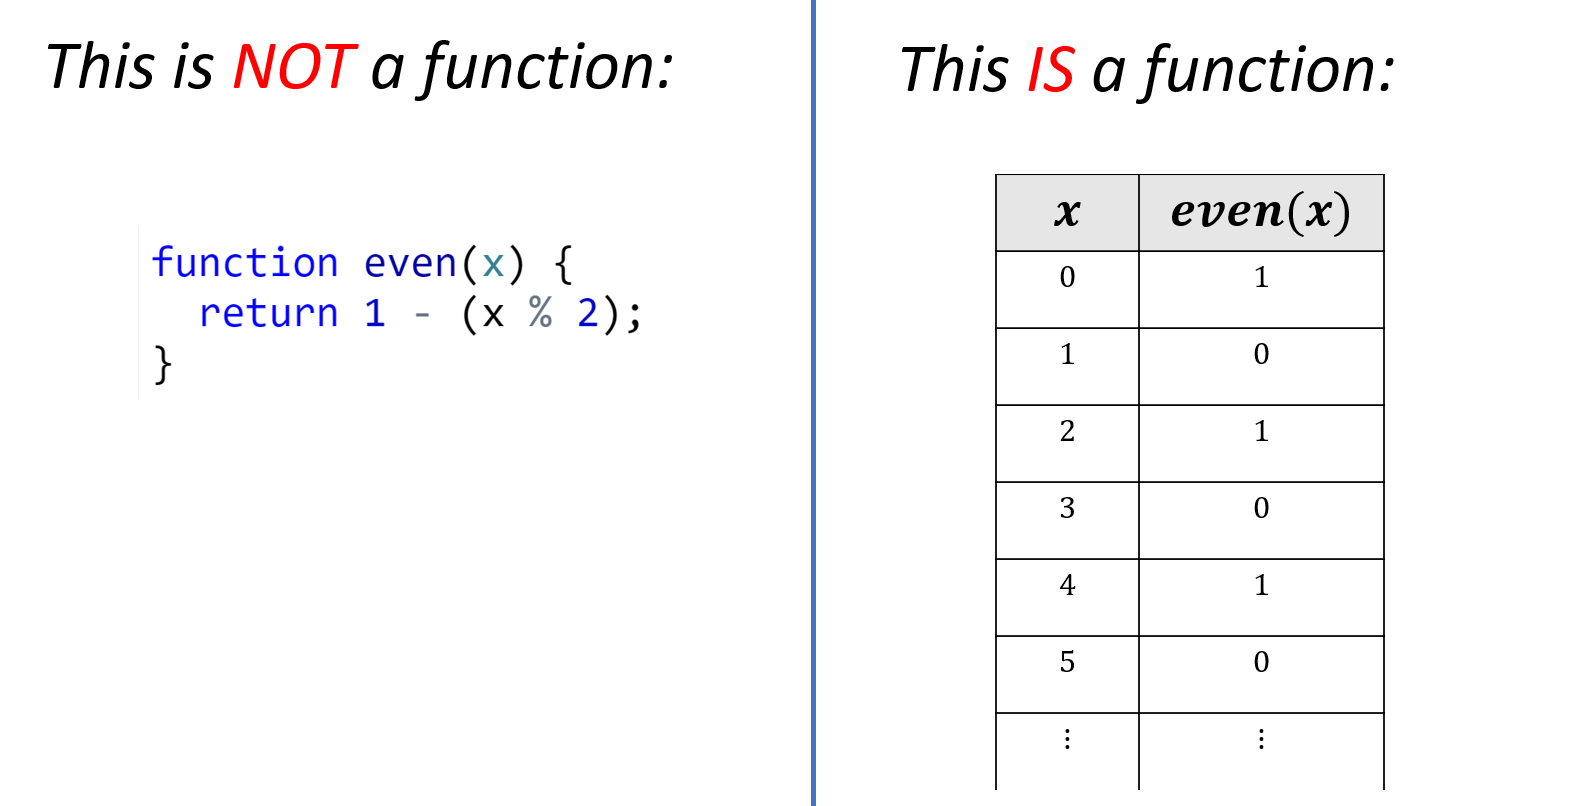
\includegraphics[width=\linewidth, height=1.5in, keepaspectratio]{../figure/functionornot.png}
\caption{A \emph{function} is a mapping of inputs to outputs. A
\emph{program} is a set of instructions on how to obtain an output given
an input. A program \emph{computes} a function, but it is not the same
as a function, popular programming language terminology
notwithstanding.}
\label{functionornotfig}
\end{marginfigure}

\hypertarget{functionprogramidea}{}
\begin{bigidea} \label[bigidea]{functionprogramidea}

A \emph{function} is not the same as a \emph{program}. A program
\emph{computes} a function.

\end{bigidea}

Distinguishing \emph{functions} from \emph{programs} (or other ways for
computing, including \emph{circuits} and \emph{machines}) is a crucial
theme for this course. For this reason, this is often a running theme in
questions that I (and many other instructors) assign in homework and
exams (hint, hint).

\hypertarget{beyonfdunc}{}
\begin{remark}[Computation beyond functions (advanced, optional)] \label[remark]{beyonfdunc}

Functions capture quite a lot of computational tasks, but one can
consider more general settings as well. For starters, we can and will
talk about \emph{partial} functions, that are not defined on all inputs.
When computing a partial function, we only need to worry about the
inputs on which the function is defined. Another way to say it is that
we can design an algorithm for a partial function \(F\) under the
assumption that someone ``promised'' us that all inputs \(x\) would be
such that \(F(x)\) is defined (as otherwise, we do not care about the
result). Hence such tasks are also known as \emph{promise problems}.

Another generalization is to consider \emph{relations} that may have
more than one possible admissible output. For example, consider the task
of finding any solution for a given set of equations. A \emph{relation}
\(R\) maps a string \(x\in \{0,1\}^*\) into a \emph{set of strings}
\(R(x)\) (for example, \(x\) might describe a set of equations, in which
case \(R(x)\) would correspond to the set of all solutions to \(x\)). We
can also identify a relation \(R\) with the set of pairs of strings
\((x,y)\) where \(y\in R(x)\). A computational process solves a relation
if for every \(x\in \{0,1\}^*\), it outputs some string \(y\in R(x)\).

Later in this book, we will consider even more general tasks, including
\emph{interactive} tasks, such as finding a good strategy in a game,
tasks defined using probabilistic notions, and others. However, for much
of this book, we will focus on the task of computing a function, and
often even a \emph{Boolean} function, that has only a single bit of
output. It turns out that a great deal of the theory of computation can
be studied in the context of this task, and the insights learned are
applicable in the more general settings.

\end{remark}

\begin{recap} \label[recap]{We-can-represent-objects-}

\begin{itemize}
\tightlist
\item
  We can represent objects we want to compute on using binary strings.
\item
  A representation scheme for a set of objects \(\mathcal{O}\) is a
  one-to-one map from \(\mathcal{O}\) to \(\{0,1\}^*\).
\item
  We can use prefix-free encoding to ``boost'' a representation for a
  set \(\mathcal{O}\) into representations of lists of elements in
  \(\mathcal{O}\).
\item
  A basic computational task is the task of \emph{computing a function}
  \(F:\{0,1\}^* \rightarrow \{0,1\}^*\). This task encompasses not just
  arithmetical computations such as multiplication, factoring, etc. but
  a great many other tasks arising in areas as diverse as scientific
  computing, artificial intelligence, image processing, data mining and
  many many more.
\item
  We will study the question of finding (or at least giving bounds on)
  what the \emph{best} algorithm for computing \(F\) for various
  interesting functions \(F\) is.
\end{itemize}

\end{recap}

\section{Exercises}\label{Exercises}

\begin{exercise} \label[exercise]{Which-one-of-these-object}

Which one of these objects can be represented by a binary string?

\begin{enumerate}
\def\labelenumi{\alph{enumi}.}
\item
  An integer \(x\)
\item
  An undirected graph \(G\).
\item
  A directed graph \(H\)
\item
  All of the above.
\end{enumerate}

\end{exercise}

\hypertarget{binaryrepex}{}
\begin{exercise}[Binary representation] \label[exercise]{binaryrepex}

\begin{enumerate}
\def\labelenumi{\alph{enumi}.}
\item
  Prove that the function \(NtS:\N \rightarrow \{0,1\}^*\) of the binary
  representation defined in \eqref{ntseq} satisfies that for every
  \(n\in \N\), if \(x = NtS(n)\) then
  \(|x| =1+\max(0,\floor{\log_2 n})\) and
  \(x_i = \floor{x/2^{\floor{\log_2 n}-i}} \mod 2\).
\item
  Prove that \(NtS\) is a one to one function by coming up with a
  function \(StN:\{0,1\}^* \rightarrow \N\) such that \(StN(NtS(n))=n\)
  for every \(n\in \N\).
\end{enumerate}

\end{exercise}

\hypertarget{compactrepletters}{}
\begin{exercise}[More compact than ASCII representation] \label[exercise]{compactrepletters}

The ASCII encoding can be used to encode a string of \(n\) English
letters as a \(7n\) bit binary string, but in this exercise, we ask
about finding a more compact representation for strings of English
lowercase letters.

\begin{enumerate}
\def\labelenumi{\arabic{enumi}.}
\item
  Prove that there exists a representation scheme \((E,D)\) for strings
  over the 26-letter alphabet \(\{ a, b,c,\ldots,z \}\) as binary
  strings such that for every \(n>0\) and length-\(n\) string
  \(x \in \{ a,b,\ldots,z \}^n\), the representation \(E(x)\) is a
  binary string of length at most \(4.8n+1000\). In other words, prove
  that for every \(n\), there exists a one-to-one function
  \(E:\{a,b,\ldots, z\}^n \rightarrow \{0,1\}^{\lfloor 4.8n +1000 \rfloor}\).
\item
  Prove that there exists \emph{no} representation scheme for strings
  over the alphabet \(\{ a, b,\ldots,z \}\) as binary strings such that
  for every length-\(n\) string \(x \in \{ a,b,\ldots, z\}^n\), the
  representation \(E(x)\) is a binary string of length
  \(\lfloor 4.6n+1000 \rfloor\). In other words, prove that there exists
  some \(n>0\) such that there is no one-to-one function
  \(E:\{a,b,\ldots,z \}^n \rightarrow \{0,1\}^{\lfloor 4.6n + 1000 \rfloor}\)
\item
  Python's \texttt{bz2.compress} function is a mapping from strings to
  strings, which uses the \emph{lossless} (and hence \emph{one to one})
  \href{https://en.wikipedia.org/wiki/Bzip2}{bzip2} algorithm for
  compression. After converting to lowercase, and truncating spaces and
  numbers, the text of Tolstoy's ``War and Peace'' contains
  \(n=2,517,262\). Yet, if we run \texttt{bz2.compress} on the string of
  the text of ``War and Peace'' we get a string of length
  \(k=6,274,768\) bits, which is only \(2.49n\) (and in particular much
  smaller than \(4.6n\)). Explain why this does not contradict your
  answer to the previous question.
\item
  Interestingly, if we try to apply \texttt{bz2.compress} on a
  \emph{random} string, we get much worse performance. In my
  experiments, I got a ratio of about \(4.78\) between the number of
  bits in the output and the number of characters in the input. However,
  one could imagine that one could do better and that there exists a
  company called ``Pied Piper'' with an algorithm that can losslessly
  compress a string of \(n\) random lowercase letters to fewer than
  \(4.6n\) bits.\footnote{Actually that particular fictional company
    uses a metric that focuses more on compression \emph{speed} then
    \emph{ratio}, see
    \href{https://blogs.dropbox.com/tech/2016/06/lossless-compression-with-brotli/}{here}
    and \href{https://www.jefftk.com/p/weissman-scores-useful}{here}.}
  Show that this is not the case by proving that for \emph{every}
  \(n>100\) and one to one function
  \(Encode:\{a,\ldots,z\}^{n} \rightarrow \{0,1\}^*\), if we let \(Z\)
  be the random variable \(|Encode(x)|\) (i.e., the length of
  \(Encode(x)\)) for \(x\) chosen uniformly at random from the set
  \(\{a,\ldots,z\}^n\), then the expected value of \(Z\) is at least
  \(4.6n\).
\end{enumerate}

\end{exercise}

\hypertarget{representinggraphsex}{}
\begin{exercise}[Representing graphs: upper bound] \label[exercise]{representinggraphsex}

Show that there is a string representation of directed graphs with
vertex set \([n]\) and degree at most \(10\) that uses at most
\(1000 n\log n\) bits. More formally, show the following: Suppose we
define for every \(n\in\mathbb{N}\), the set \(G_n\) as the set
containing all directed graphs (with no self loops) over the vertex set
\([n]\) where every vertex has degree at most \(10\). Then, prove that
for every sufficiently large \(n\), there exists a one-to-one function
\(E:G_n \rightarrow \{0,1\}^{\lfloor 1000 n \log n \rfloor}\).

\end{exercise}

\hypertarget{represgraphlbex}{}
\begin{exercise}[Representing graphs: lower bound] \label[exercise]{represgraphlbex}

\begin{enumerate}
\def\labelenumi{\arabic{enumi}.}
\item
  Define \(S_n\) to be the set of one-to-one and onto functions mapping
  \([n]\) to \([n]\). Prove that there is a one-to-one mapping from
  \(S_n\) to \(G_{2n}\), where \(G_{2n}\) is the set defined in
  \cref{representinggraphsex} above.
\item
  In this question you will show that one cannot improve the
  representation of \cref{representinggraphsex} to length
  \(o(n \log n)\). Specifically, prove for every sufficiently large
  \(n\in \mathbb{N}\) there is \emph{no} one-to-one function
  \(E:G_n \rightarrow \{0,1\}^{\lfloor 0.001 n \log n \rfloor +1000}\).
\end{enumerate}

\end{exercise}

\hypertarget{multrepres}{}
\begin{exercise}[Multiplying in different representation] \label[exercise]{multrepres}

Recall that the grade-school algorithm for multiplying two numbers
requires \(O(n^2)\) operations. Suppose that instead of using decimal
representation, we use one of the following representations \(R(x)\) to
represent a number \(x\) between \(0\) and \(10^n-1\). For which one of
these representations you can still multiply the numbers in \(O(n^2)\)
operations?

\begin{enumerate}
\def\labelenumi{\alph{enumi}.}
\item
  The standard binary representation: \(B(x)=(x_0,\ldots,x_{k})\) where
  \(x = \sum_{i=0}^{k} x_i 2^i\) and \(k\) is the largest number s.t.
  \(x \geq 2^k\).
\item
  The reverse binary representation: \(B(x) = (x_{k},\ldots,x_0)\) where
  \(x_i\) is defined as above for \(i=0,\ldots,k-1\).\\
\item
  Binary coded decimal representation: \(B(x)=(y_0,\ldots,y_{n-1})\)
  where \(y_i \in \{0,1\}^4\) represents the \(i^{th}\) decimal digit of
  \(x\) mapping \(0\) to \(0000\), \(1\) to \(0001\), \(2\) to \(0010\),
  etc. (i.e.~\(9\) maps to \(1001\))
\item
  All of the above.
\end{enumerate}

\end{exercise}

\begin{exercise} \label[exercise]{Suppose-that-RN-rightarro}

Suppose that \(R:\N \rightarrow \{0,1\}^*\) corresponds to representing
a number \(x\) as a string of \(x\) \(1\)'s, (e.g., \(R(4)=1111\),
\(R(7)=1111111\), etc.). If \(x,y\) are numbers between \(0\) and
\(10^n -1\), can we still multiply \(x\) and \(y\) using \(O(n^2)\)
operations if we are given them in the representation \(R(\cdot)\)?

\end{exercise}

\begin{exercise} \label[exercise]{Recall-that-if-F-is-a-one}

Recall that if \(F\) is a one-to-one and onto function mapping elements
of a finite set \(U\) into a finite set \(V\) then the sizes of \(U\)
and \(V\) are the same. Let \(B:\N\rightarrow\{0,1\}^*\) be the function
such that for every \(x\in\N\), \(B(x)\) is the binary representation of
\(x\).

\begin{enumerate}
\def\labelenumi{\arabic{enumi}.}
\item
  Prove that \(x < 2^k\) if and only if \(|B(x)| \leq k\).
\item
  Use 1. to compute the size of the set
  \(\{ y \in \{0,1\}^* : |y| \leq k \}\) where \(|y|\) denotes the
  length of the string \(y\).
\item
  Use 1. and 2. to prove that \(2^k-1 = 1 + 2 + 4+ \cdots + 2^{k-1}\).
\end{enumerate}

\end{exercise}

\hypertarget{prefix-free-tuples-ex}{}
\begin{exercise}[Prefix-free encoding of tuples] \label[exercise]{prefix-free-tuples-ex}

Suppose that \(F:\N\rightarrow\{0,1\}^*\) is a one-to-one function that
is \emph{prefix-free} in the sense that there is no \(a\neq b\) s.t.
\(F(a)\) is a prefix of \(F(b)\).

\begin{enumerate}
\def\labelenumi{\alph{enumi}.}
\item
  Prove that \(F_2:\N\times \N \rightarrow \{0,1\}^*\), defined as
  \(F_2(a,b) = F(a)F(b)\) (i.e., the concatenation of \(F(a)\) and
  \(F(b)\)) is a one-to-one function.
\item
  Prove that \(F_*:\N^*\rightarrow\{0,1\}^*\) defined as
  \(F_*(a_1,\ldots,a_k) = F(a_1)\cdots F(a_k)\) is a one-to-one
  function, where \(\N^*\) denotes the set of all finite-length lists of
  natural numbers.
\end{enumerate}

\end{exercise}

\hypertarget{prefix-free-ex}{}
\begin{exercise}[More efficient prefix-free transformation] \label[exercise]{prefix-free-ex}

Suppose that \(F:O\rightarrow\{0,1\}^*\) is some (not necessarily
prefix-free) representation of the objects in the set \(O\), and
\(G:\N\rightarrow\{0,1\}^*\) is a prefix-free representation of the
natural numbers. Define \(F'(o)=G(|F(o)|)F(o)\) (i.e., the concatenation
of the representation of the length \(F(o)\) and \(F(o)\)).

\begin{enumerate}
\def\labelenumi{\alph{enumi}.}
\item
  Prove that \(F'\) is a prefix-free representation of \(O\).
\item
  Show that we can transform any representation to a prefix-free one by
  a modification that takes a \(k\) bit string into a string of length
  at most \(k+O(\log k)\).
\item
  Show that we can transform any representation to a prefix-free one by
  a modification that takes a \(k\) bit string into a string of length
  at most \(k+ \log k + O(\log\log k)\).\footnote{Hint: Think
    recursively how to represent the length of the string.}
\end{enumerate}

\end{exercise}

\hypertarget{prefix-free-lb}{}
\begin{exercise}[Kraft's Inequality] \label[exercise]{prefix-free-lb}

Suppose that \(S \subseteq \{0,1\}^n\) is some finite prefix-free set.

\begin{enumerate}
\def\labelenumi{\alph{enumi}.}
\item
  For every \(k \leq n\) and length-\(k\) string \(x\in S\), let
  \(L(x) \subseteq \{0,1\}^n\) denote all the length-\(n\) strings whose
  first \(k\) bits are \(x_0,\ldots,x_{k-1}\). Prove that \textbf{(1)}
  \(|L(x)|=2^{n-|x|}\) and \textbf{(2)} If \(x \neq x'\) then \(L(x)\)
  is disjoint from \(L(x')\).
\item
  Prove that \(\sum_{x\in S}2^{-|x|} \leq 1\).
\item
  Prove that there is no prefix-free encoding of strings with less than
  logarithmic overhead. That is, prove that there is no function
  \(\ensuremath{\mathit{PF}}:\{0,1\}^* \rightarrow \{0,1\}^*\) s.t.
  \(|\ensuremath{\mathit{PF}}(x)| \leq |x|+0.9\log |x|\) for every
  \(x\in \{0,1\}^*\) and such that the set
  \(\{ \ensuremath{\mathit{PF}}(x) : x\in \{0,1\}^* \}\) is prefix-free.
  The factor \(0.9\) is arbitrary; all that matters is that it is less
  than \(1\).
\end{enumerate}

\end{exercise}

\hypertarget{onetoonecompex}{}
\begin{exercise}[Composition of one-to-one functions] \label[exercise]{onetoonecompex}

Prove that for every two one-to-one functions \(F:S \rightarrow T\) and
\(G:T \rightarrow U\), the function \(H:S \rightarrow U\) defined as
\(H(x)=G(F(x))\) is one to one.

\end{exercise}

\hypertarget{naturalsstringsmapex}{}
\begin{exercise}[Natural numbers and strings] \label[exercise]{naturalsstringsmapex}

\begin{enumerate}
\def\labelenumi{\arabic{enumi}.}
\item
  We have shown that the natural numbers can be represented as strings.
  Prove that the other direction holds as well: that there is a
  one-to-one map \(StN:\{0,1\}^* \rightarrow \N\). (\(StN\) stands for
  ``strings to numbers.'')
\item
  Recall that Cantor proved that there is no one-to-one map
  \(RtN:\R \rightarrow \N\). Show that Cantor's result implies
  \cref{cantorthm}.
\end{enumerate}

\end{exercise}

\hypertarget{listsinttonumex}{}
\begin{exercise}[Map lists of integers to a number] \label[exercise]{listsinttonumex}

Recall that for every set \(S\), the set \(S^*\) is defined as the set
of all finite sequences of members of \(S\) (i.e.,
\(S^* = \{ (x_0,\ldots,x_{n-1}) \;|\; n\in\mathbb{N} \;,\; \forall_{i\in [n]} x_i \in S \}\)
). Prove that there is a one-one-map from \(\mathbb{Z}^*\) to
\(\mathbb{N}\) where \(\mathbb{Z}\) is the set of
\(\{ \ldots, -3 , -2 , -1,0,+1,+2,+3,\ldots \}\) of all integers.

\end{exercise}

\section{Bibliographical notes}\label{bibnotesrepres}

The study of representing data as strings, including issues such as
\emph{compression} and \emph{error corrections} falls under the purview
of \emph{information theory}, as covered in the classic textbook of
Cover and Thomas \cite{CoverThomas06}. Representations are also studied
in the field of \emph{data structures design}, as covered in texts such
as \cite{CLRS}.

The question of whether to represent integers with the most significant
digit first or last is known as
\href{https://betterexplained.com/articles/understanding-big-and-little-endian-byte-order/}{Big
Endian vs.~Little Endian} representation. This terminology comes from
Cohen's \cite{cohen1981holy} entertaining and informative paper about
the conflict between adherents of both schools which he compared to the
warring tribes in Jonathan Swift's \emph{``Gulliver's Travels''}. The
two's complement representation of signed integers was suggested in von
Neumann's classic report \cite{vonNeumann45} that detailed the design
approaches for a stored-program computer, though similar representations
have been used even earlier in abacus and other mechanical computation
devices.

The idea that we should separate the \emph{definition} or
\emph{specification} of a function from its \emph{implementation} or
\emph{computation} might seem ``obvious,'' but it took quite a lot of
time for mathematicians to arrive at this viewpoint. Historically, a
function \(F\) was identified by rules or formulas showing how to derive
the output from the input. As we discuss in greater depth in
\cref{chapcomputable}, in the 1800s this somewhat informal notion of a
function started ``breaking at the seams,'' and eventually
mathematicians arrived at the more rigorous definition of a function as
an arbitrary assignment of input to outputs. While many functions may be
described (or computed) by one or more formulas, today we do not
consider that to be an essential property of functions, and also allow
functions that do not correspond to any ``nice'' formula.

We have mentioned that all representations of the real numbers are
inherently \emph{approximate}. Thus an important endeavor is to
understand what guarantees we can offer on the approximation quality of
the output of an algorithm, as a function of the approximation quality
of the inputs. This question is known as the question of determining the
\href{https://en.wikipedia.org/wiki/Numerical_stability}{numerical
stability} of given equations. The
\href{https://floating-point-gui.de/}{Floating Points Guide website}
contains an extensive description of the floating point representation,
as well the many ways in which it could subtly fail, see also the
website \href{http://0.30000000000000004.com/}{0.30000000000000004.com}.

Dauben \cite{Dauben90cantor} gives a biography of Cantor with emphasis
on the development of his mathematical ideas. \cite{halmos1960naive} is
a classic textbook on set theory, including also Cantor's theorem.
Cantor's Theorem is also covered in many texts on discrete mathematics,
including \cite{LehmanLeightonMeyer , LewisZax19 }.

The adjacency matrix representation of graphs is not merely a convenient
way to map a graph into a binary string, but it turns out that many
natural notions and operations on matrices are useful for graphs as
well. (For example, Google's PageRank algorithm relies on this
viewpoint.) The notes of
\href{http://www.cs.yale.edu/homes/spielman/561/}{Spielman's course} are
an excellent source for this area, known as \emph{spectral graph
theory}. We will return to this view much later in this book when we
talk about \emph{random walks}.


\part{Finite computation}

\chapter{Defining computation}\label{compchap}

\begin{objectives} \label[objectives]{See-that-computation-can-}

\begin{itemize}
\tightlist
\item
  See that computation can be precisely modeled.\\
\item
  Learn the computational model of \emph{Boolean circuits} /
  \emph{straight-line programs}.
\item
  Equivalence of circuits and straight-line programs.
\item
  Equivalence of AND/OR/NOT and NAND.
\item
  Examples of computing in the physical world.\\
\end{itemize}

\end{objectives}

\begin{quote}
\emph{``there is no reason why mental as well as bodily labor should not
be economized by the aid of machinery''}, Charles Babbage, 1852
\end{quote}

\begin{quote}
\emph{``If, unwarned by my example, any man shall undertake and shall
succeed in constructing an engine embodying in itself the whole of the
executive department of mathematical analysis upon different principles
or by simpler mechanical means, I have no fear of leaving my reputation
in his charge, for he alone will be fully able to appreciate the nature
of my efforts and the value of their results.''}, Charles Babbage, 1864
\end{quote}

\begin{quote}
\emph{``To understand a program you must become both the machine and the
program.''}, Alan Perlis, 1982
\end{quote}


\begin{marginfigure}
\centering
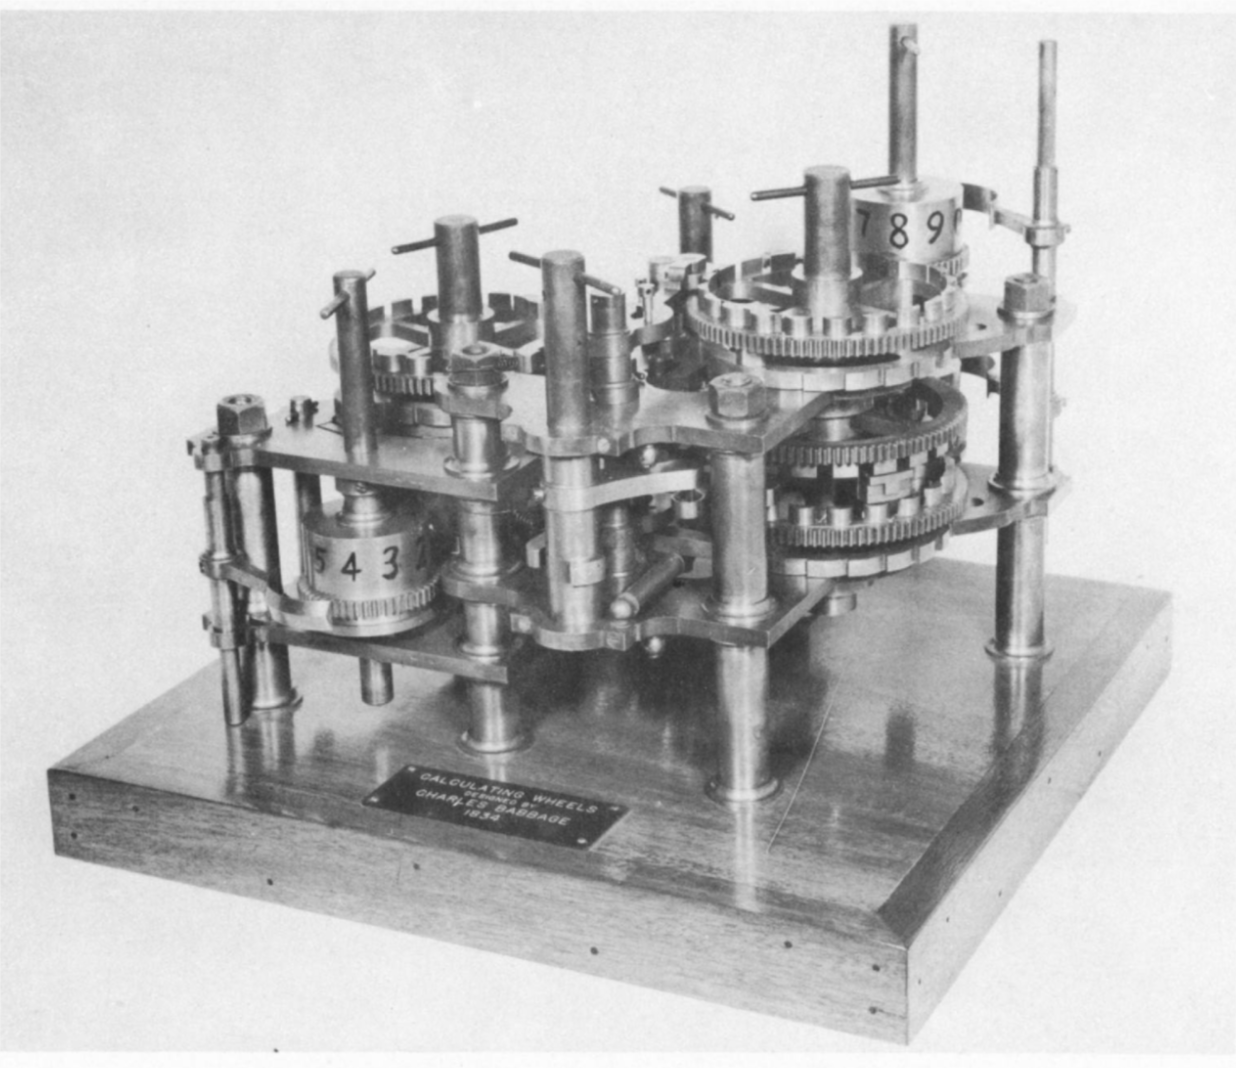
\includegraphics[width=\linewidth, height=1.5in, keepaspectratio]{../figure/wheels_babbage.png}
\caption{Calculating wheels by Charles Babbage. Image taken from the
Mark I `operating manual'}
\label{babbagewheels}
\end{marginfigure}


\begin{marginfigure}
\centering
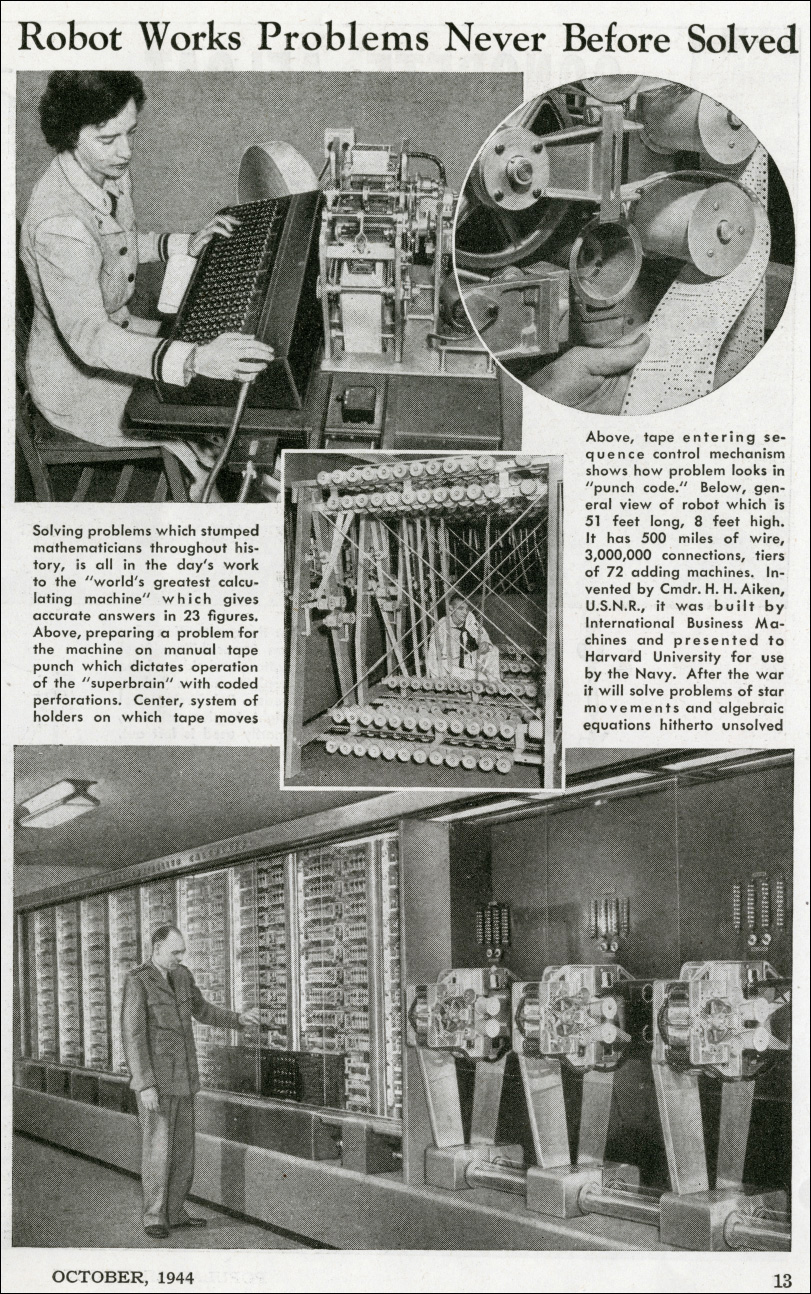
\includegraphics[width=\linewidth, height=1.5in, keepaspectratio]{../figure/PopularMechanics1944smaller.jpg}
\caption{A 1944 \emph{Popular Mechanics} article on the
\href{http://sites.harvard.edu/~chsi/markone/about.html}{Harvard Mark I
computer}.}
\label{markIcomp}
\end{marginfigure}

People have been computing for thousands of years, with aids that
include not just pen and paper, but also abacus, slide rules, various
mechanical devices, and modern electronic computers. A priori, the
notion of computation seems to be tied to the particular mechanism that
you use. You might think that the ``best'' algorithm for multiplying
numbers will differ if you implement it in \emph{Python} on a modern
laptop than if you use pen and paper. However, as we saw in the
introduction (\cref{chapintro}), an algorithm that is asymptotically
better would eventually beat a worse one regardless of the underlying
technology. This gives us hope for a \emph{technology independent} way
of defining computation. This is what we do in this chapter. We will
define the notion of computing an output from an input by applying a
sequence of basic operations (see \cref{compchapwhatvshowfig}). Using
this, we will be able to precisely define statements such as ``function
\(f\) can be computed by model \(X\)'' or ``function \(f\) can be
computed by model \(X\) using \(s\) operations''.


\begin{figure}
\centering
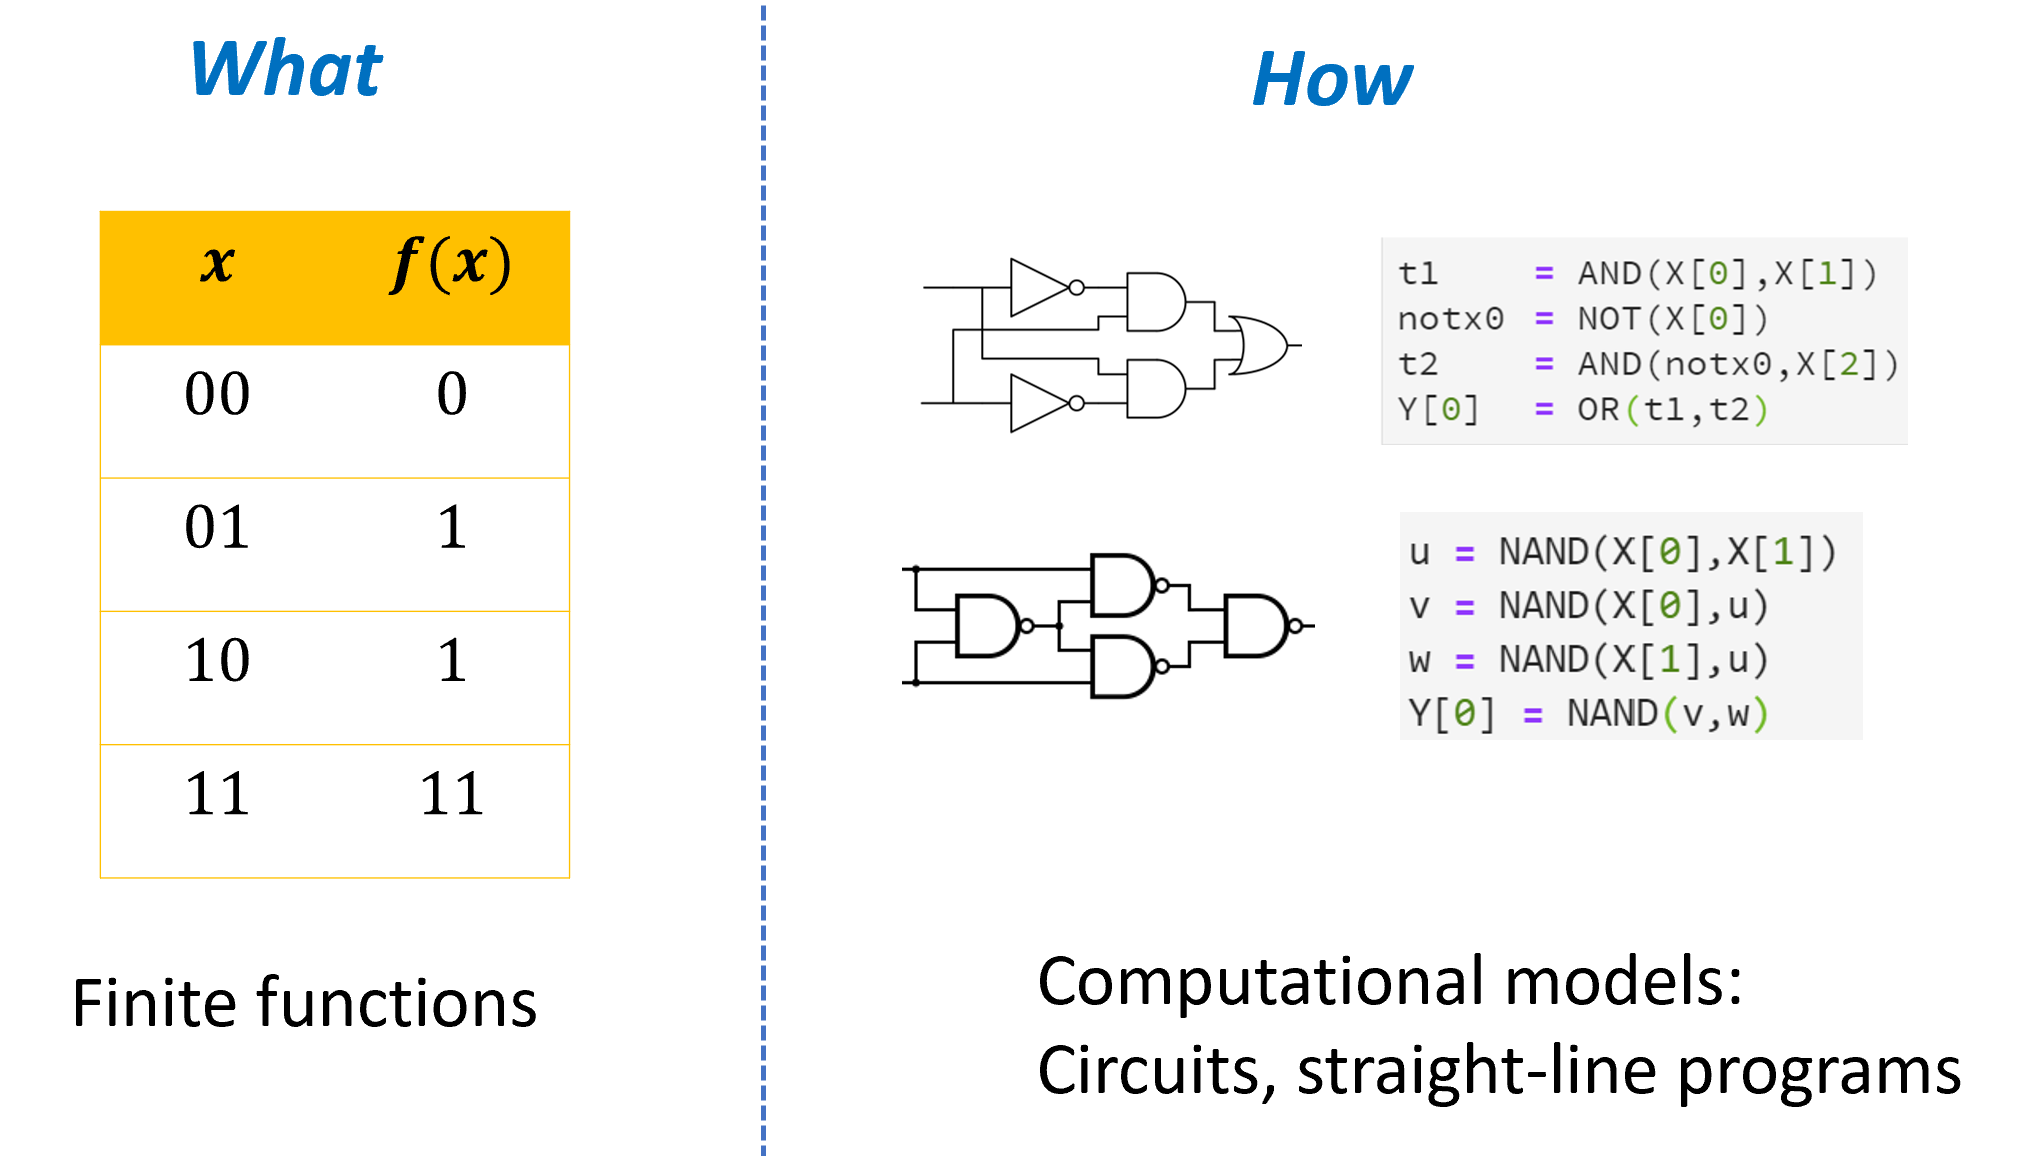
\includegraphics[width=\textwidth, height=0.25\paperheight, keepaspectratio]{../figure/compchapterwhatvshow.png}
\caption{A function mapping strings to strings \emph{specifies} a
computational task, i.e., describes \emph{what} the desired relation
between the input and the output is. In this chapter we define models
for \emph{implementing} computational processes that achieve the desired
relation, i.e., describe \emph{how} to compute the output from the
input. We will see several examples of such models using both Boolean
circuits and straight-line programming languages.}
\label{compchapwhatvshowfig}
\end{figure}

\section{Defining computation}\label{Defining-computation}

The name ``algorithm'' is derived from the Latin transliteration of
Muhammad ibn Musa al-Khwarizmi's name. Al-Khwarizmi was a Persian
scholar during the 9th century whose books introduced the western world
to the decimal positional numeral system, as well as to the solutions of
linear and quadratic equations (see \cref{alKhwarizmi}). However
Al-Khwarizmi's descriptions of algorithms were rather informal by
today's standards. Rather than use ``variables'' such as \(x,y\), he
used concrete numbers such as 10 and 39, and trusted the reader to be
able to extrapolate from these examples, much as algorithms are still
taught to children today.

Here is how Al-Khwarizmi described the algorithm for solving an equation
of the form \(x^2 +bx = c\):

\begin{quote}
\emph{{[}How to solve an equation of the form {]} ``roots and squares
are equal to numbers'': For instance ``one square , and ten roots of the
same, amount to thirty-nine dirhems'' that is to say, what must be the
square which, when increased by ten of its own root, amounts to
thirty-nine? The solution is this: you halve the number of the roots,
which in the present instance yields five. This you multiply by itself;
the product is twenty-five. Add this to thirty-nine' the sum is
sixty-four. Now take the root of this, which is eight, and subtract from
it half the number of roots, which is five; the remainder is three. This
is the root of the square which you sought for; the square itself is
nine.}
\end{quote}


\begin{marginfigure}
\centering
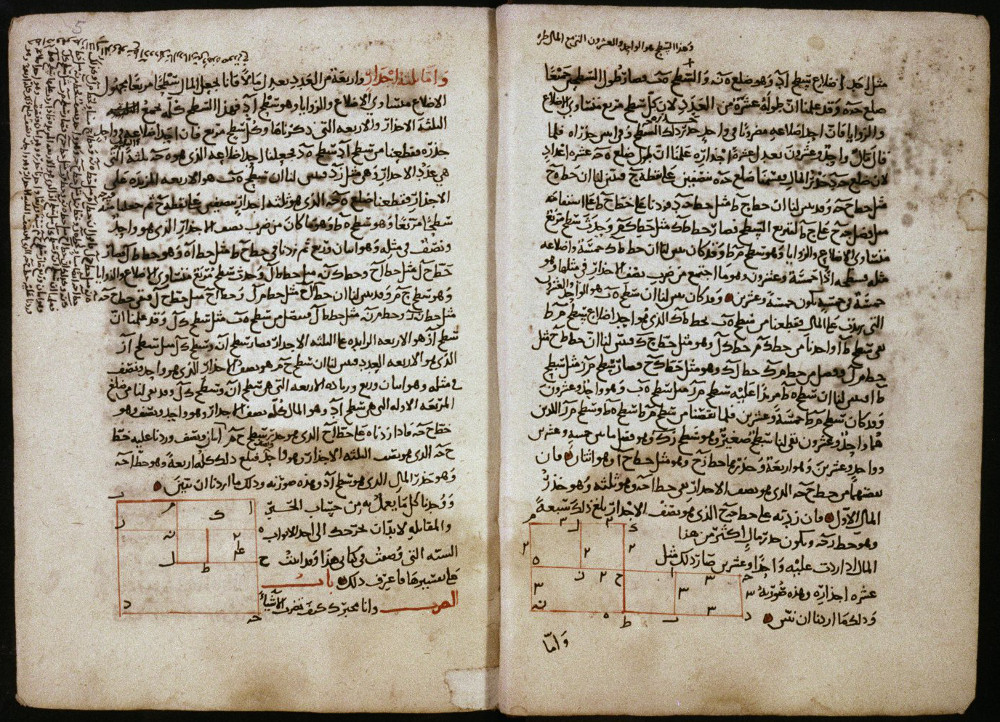
\includegraphics[width=\linewidth, height=1.5in, keepaspectratio]{../figure/alKhwarizmi.jpg}
\caption{Text pages from Algebra manuscript with geometrical solutions
to two quadratic equations. Shelfmark: MS. Huntington 214
fol.~004v-005r}
\label{alKhwarizmi}
\end{marginfigure}


\begin{marginfigure}
\centering
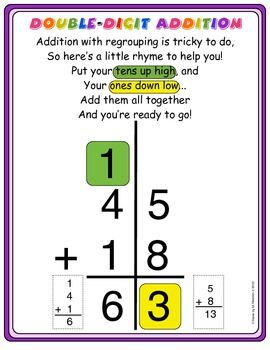
\includegraphics[width=\linewidth, height=1.5in, keepaspectratio]{../figure/addition_regrouping.jpg}
\caption{An explanation for children of the two digit addition
algorithm}
\label{childrenalg}
\end{marginfigure}

For the purposes of this book, we will need a much more precise way to
describe algorithms. Fortunately (or is it unfortunately?), at least at
the moment, computers lag far behind school-age children in learning
from examples. Hence in the 20th century, people came up with exact
formalisms for describing algorithms, namely \emph{programming
languages}. Here is al-Khwarizmi's quadratic equation solving algorithm
described in the \emph{Python} programming language:

\begin{code}
from math import sqrt
#Pythonspeak to enable use of the sqrt function to compute square roots.

def solve_eq(b,c):
    # return solution of x^2 + bx = c following Al Khwarizmi's instructions
    # Al Kwarizmi demonstrates this for the case b=10 and c= 39

    val1 = b / 2.0 # "halve the number of the roots"
    val2 = val1 * val1 # "this you multiply by itself"
    val3 = val2 + c # "Add this to thirty-nine"
    val4 = sqrt(val3) # "take the root of this"
    val5 = val4 - val1 # "subtract from it half the number of roots"
    return val5  # "This is the root of the square which you sought for"

# Test: solve x^2 + 10*x = 39
print(solve_eq(10,39))
# 3.0
\end{code}

We can define algorithms informally as follows:

\begin{quote} \label[quote]{Informal-definition-of-an}

\textbf{Informal definition of an algorithm:} An \emph{algorithm} is a
set of instructions for how to compute an output from an input by
following a sequence of ``elementary steps''.

An algorithm \(A\) \emph{computes} a function \(F\) if for every input
\(x\), if we follow the instructions of \(A\) on the input \(x\), we
obtain the output \(F(x)\).

\end{quote}

In this chapter we will make this informal definition precise using the
model of \textbf{Boolean Circuits}. We will show that Boolean Circuits
are equivalent in power to \textbf{straight line programs} that are
written in ``ultra simple'' programming languages that do not even have
loops. We will also see that the particular choice of \textbf{elementary
operations} is immaterial and many different choices yield models with
equivalent power (see \cref{compchapoverviewfig}). However, it will take
us some time to get there. We will start by discussing what are
``elementary operations'' and how we map a description of an algorithm
into an actual physical process that produces an output from an input in
the real world.


\begin{figure}
\centering
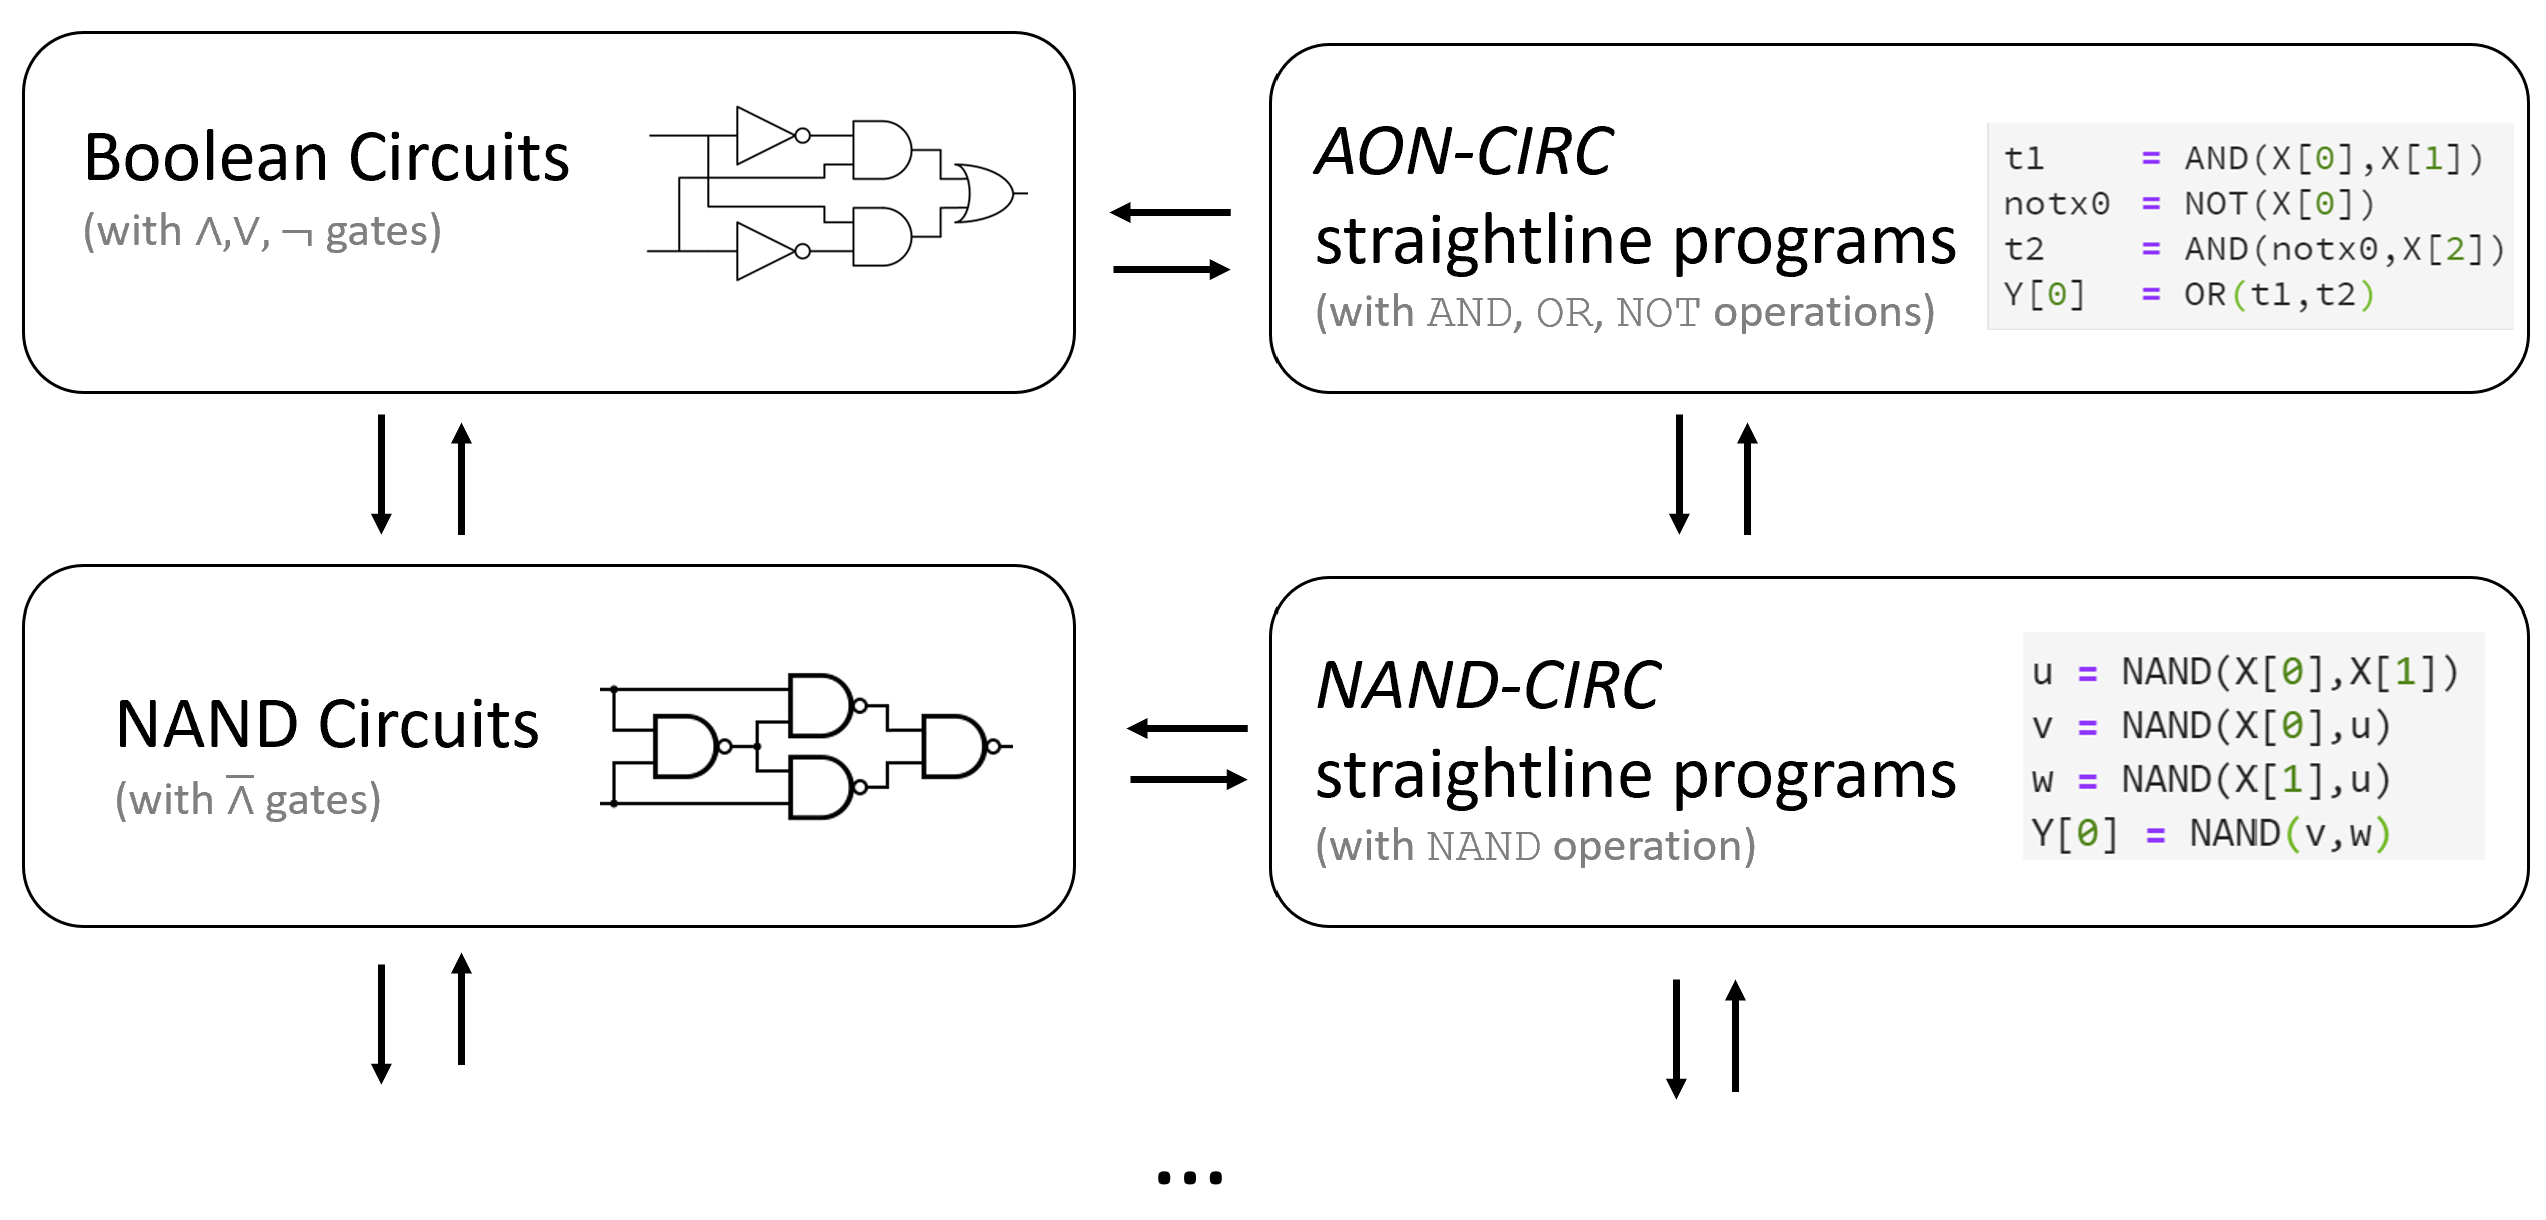
\includegraphics[width=\textwidth, height=0.25\paperheight, keepaspectratio]{../figure/compcharoverview.png}
\caption{An overview of the computational models defined in this
chapter. We will show several equivalent ways to represent a recipe for
performing a finite computation. Specifically we will show that we can
model such a computation using either a \emph{Boolean circuit} or a
\emph{straight line program}, and these two representations are
equivalent to one another. We will also show that we can choose as our
basic operations either the set
\(\{ \ensuremath{\mathit{AND}} , \ensuremath{\mathit{OR}} , \ensuremath{\mathit{NOT}} \}\)
or the set \(\{ \ensuremath{\mathit{NAND}} \}\) and these two choices
are equivalent in power. By making the choice of whether to use circuits
or programs, and whether to use
\(\{ \ensuremath{\mathit{AND}} , \ensuremath{\mathit{OR}} , \ensuremath{\mathit{NOT}} \}\)
or \(\{ \ensuremath{\mathit{NAND}} \}\) we obtain four equivalent ways
of modeling finite computation. Moreover, there are many other choices
of sets of basic operations that are equivalent in power.}
\label{compchapoverviewfig}
\end{figure}

\section{Computing using AND, OR, and
NOT.}\label{Computing-using-AND-OR-an}

An algorithm breaks down a \emph{complex} calculation into a series of
\emph{simpler} steps. These steps can be executed in a variety of
different ways, including:

\begin{itemize}
\item
  Writing down symbols on a piece of paper.
\item
  Modifying the current flowing on electrical wires.
\item
  Binding a protein to a strand of DNA.
\item
  Responding to a stimulus by a member of a collection (e.g., a bee in a
  colony, a trader in a market).
\end{itemize}

To formally define algorithms, let us try to ``err on the side of
simplicity'' and model our ``basic steps'' as truly minimal. For
example, here are some very simple functions:

\begin{itemize}
\tightlist
\item
  \(\ensuremath{\mathit{OR}}:\{0,1\}^2 \rightarrow \{0,1\}\) defined as
\end{itemize}

\[\ensuremath{\mathit{OR}}(a,b) = \begin{cases} 0 & a=b=0 \\ 1 & \text{otherwise} \end{cases}\]

\begin{itemize}
\tightlist
\item
  \(\ensuremath{\mathit{AND}}:\{0,1\}^2 \rightarrow \{0,1\}\) defined as
\end{itemize}

\[\ensuremath{\mathit{AND}}(a,b) = \begin{cases} 1 & a=b=1 \\ 0 & \text{otherwise} \end{cases}\]

\begin{itemize}
\tightlist
\item
  \(\ensuremath{\mathit{NOT}}:\{0,1\} \rightarrow \{0,1\}\) defined as
\end{itemize}

\[\ensuremath{\mathit{NOT}}(a) = \begin{cases} 0 & a = 1 \\ 1 & a = 0 \end{cases}\]

The functions \(\ensuremath{\mathit{AND}}\),
\(\ensuremath{\mathit{OR}}\) and \(\ensuremath{\mathit{NOT}}\), are the
basic logical operators used in logic and many computer systems. In the
context of logic, it is common to use the notation \(a \wedge b\) for
\(\ensuremath{\mathit{AND}}(a,b)\), \(a \vee b\) for
\(\ensuremath{\mathit{OR}}(a,b)\) and \(\overline{a}\) and \(\neg a\)
for \(\ensuremath{\mathit{NOT}}(a)\), and we will use this notation as
well.

Each one of the functions
\(\ensuremath{\mathit{AND}},\ensuremath{\mathit{OR}},\ensuremath{\mathit{NOT}}\)
takes either one or two single bits as input, and produces a single bit
as output. Clearly, it cannot get much more basic than that. However,
the power of computation comes from \emph{composing} such simple
building blocks together.

\hypertarget{majorityfunctionex}{}
\begin{example}[Majority from $AND$,$OR$ and $NOT$] \label[example]{majorityfunctionex}

Consider the function
\(\ensuremath{\mathit{MAJ}}:\{0,1\}^3 \rightarrow \{0,1\}\) that is
defined as follows:

\[\ensuremath{\mathit{MAJ}}(x) = \begin{cases}1 & x_0 + x_1 + x_2 \geq 2 \\ 0 & \text{otherwise}\end{cases} \;.\]

That is, for every \(x\in \{0,1\}^3\),
\(\ensuremath{\mathit{MAJ}}(x)=1\) if and only if the majority (i.e., at
least two out of the three) of \(x\)'s elements are equal to \(1\). Can
you come up with a formula involving \(\ensuremath{\mathit{AND}}\),
\(\ensuremath{\mathit{OR}}\) and \(\ensuremath{\mathit{NOT}}\) to
compute \(\ensuremath{\mathit{MAJ}}\)? (It would be useful for you to
pause at this point and work out the formula for yourself. As a hint,
although the \(\ensuremath{\mathit{NOT}}\) operator is needed to compute
some functions, you will not need to use it to compute
\(\ensuremath{\mathit{MAJ}}\).)

Let us first try to rephrase \(\ensuremath{\mathit{MAJ}}(x)\) in words:
``\(\ensuremath{\mathit{MAJ}}(x)=1\) if and only if there exists some
pair of distinct elements \(i,j\) such that both \(x_i\) and \(x_j\) are
equal to \(1\).'' In other words it means that
\(\ensuremath{\mathit{MAJ}}(x)=1\) iff \emph{either} both \(x_0=1\)
\emph{and} \(x_1=1\), \emph{or} both \(x_1=1\) \emph{and} \(x_2=1\),
\emph{or} both \(x_0=1\) \emph{and} \(x_2=1\). Since the
\(\ensuremath{\mathit{OR}}\) of three conditions \(c_0,c_1,c_2\) can be
written as
\(\ensuremath{\mathit{OR}}(c_0,\ensuremath{\mathit{OR}}(c_1,c_2))\), we
can now translate this into a formula as follows:

\[
\ensuremath{\mathit{MAJ}}(x_0,x_1,x_2) = \ensuremath{\mathit{OR}}\left(\, \ensuremath{\mathit{AND}}(x_0,x_1)\;,\; \ensuremath{\mathit{OR}} \bigl( \ensuremath{\mathit{AND}}(x_1,x_2) \;,\; \ensuremath{\mathit{AND}}(x_0,x_2) \bigr) \, \right) \;. \label{eqmajandornot}
\]

Recall that we can also write \(a \vee b\) for
\(\ensuremath{\mathit{OR}}(a,b)\) and \(a \wedge b\) for
\(\ensuremath{\mathit{AND}}(a,b)\). With this notation,
\eqref{eqmajandornot} can also be written as

\[\ensuremath{\mathit{MAJ}}(x_0,x_1,x_2) = ((x_0 \wedge x_1) \vee (x_1 \wedge x_2)) \vee (x_0 \wedge x_2)\;.\]

We can also write \eqref{eqmajandornot} in a ``programming language''
format, expressing it as a set of instructions for computing
\(\ensuremath{\mathit{MAJ}}\) given the basic operations
\(\ensuremath{\mathit{AND}},\ensuremath{\mathit{OR}},\ensuremath{\mathit{NOT}}\):

\begin{code}
def MAJ(X[0],X[1],X[2]):
    firstpair  = AND(X[0],X[1])
    secondpair = AND(X[1],X[2])
    thirdpair  = AND(X[0],X[2])
    temp       = OR(secondpair,thirdpair)
    return OR(firstpair,temp)
\end{code}

\end{example}

\subsection{Some properties of AND and
OR}\label{Some-properties-of-AND-an}

Like standard addition and multiplication, the functions
\(\ensuremath{\mathit{AND}}\) and \(\ensuremath{\mathit{OR}}\) satisfy
the properties of \emph{commutativity}: \(a \vee b = b \vee a\) and
\(a \wedge b = b \wedge a\) and \emph{associativity}:
\((a \vee b) \vee c = a \vee (b \vee c)\) and
\((a \wedge b) \wedge c = a \wedge (b \wedge c)\). As in the case of
addition and multiplication, we often drop the parenthesis and write
\(a \vee b \vee c \vee d\) for \(((a \vee b) \vee c) \vee d\), and
similarly OR's and AND's of more terms. They also satisfy a variant of
the distributive law:

\hypertarget{distributivelaw}{}
\begin{solvedexercise}[Distributive law for AND and OR] \label[solvedexercise]{distributivelaw}

Prove that for every \(a,b,c \in \{0,1\}\),
\(a \wedge (b \vee c) = (a \wedge b) \vee (a \wedge c)\).

\end{solvedexercise}

\begin{solution} \label[solution]{We-can-prove-this-by-enum}

We can prove this by enumerating over all the \(8\) possible values for
\(a,b,c \in \{0,1\}\) but it also follows from the standard distributive
law. Suppose that we identify any positive integer with ``true'' and the
value zero with ``false''. Then for every numbers \(u,v \in \N\),
\(u+v\) is positive if and only if \(u \vee v\) is true and
\(u \cdot v\) is positive if and only if \(u \wedge v\) is true. This
means that for every \(a,b,c \in \{0,1\}\), the expression
\(a \wedge (b \vee c)\) is true if and only if \(a \cdot(b+c)\) is
positive, and the expression \((a \wedge b) \vee (a \wedge c)\) is true
if and only if \(a \cdot b + a \cdot c\) is positive, But by the
standard distributive law \(a\cdot (b+c) = a\cdot b + a \cdot c\) and
hence the former expression is true if and only if the latter one is.

\end{solution}

\subsection{Extended example: Computing \(\ensuremath{\mathit{XOR}}\)
from \(\ensuremath{\mathit{AND}}\), \(\ensuremath{\mathit{OR}}\), and
\(\ensuremath{\mathit{NOT}}\)}\label{xoraonexample}

Let us see how we can obtain a different function from the same building
blocks. Define
\(\ensuremath{\mathit{XOR}}:\{0,1\}^2 \rightarrow \{0,1\}\) to be the
function \(\ensuremath{\mathit{XOR}}(a,b)= a + b \mod 2\). That is,
\(\ensuremath{\mathit{XOR}}(0,0)=\ensuremath{\mathit{XOR}}(1,1)=0\) and
\(\ensuremath{\mathit{XOR}}(1,0)=\ensuremath{\mathit{XOR}}(0,1)=1\). We
claim that we can construct \(\ensuremath{\mathit{XOR}}\) using only
\(\ensuremath{\mathit{AND}}\), \(\ensuremath{\mathit{OR}}\), and
\(\ensuremath{\mathit{NOT}}\).

\begin{pause} \label[pause]{As-usual-it-is-a-good-exe}

As usual, it is a good exercise to try to work out the algorithm for
\(\ensuremath{\mathit{XOR}}\) using \(\ensuremath{\mathit{AND}}\),
\(\ensuremath{\mathit{OR}}\) and \(\ensuremath{\mathit{NOT}}\) on your
own before reading further.

\end{pause}

The following algorithm computes \(\ensuremath{\mathit{XOR}}\) using
\(\ensuremath{\mathit{AND}}\), \(\ensuremath{\mathit{OR}}\), and
\(\ensuremath{\mathit{NOT}}\):

\begin{algorithm}[$XOR$ from $AND$/$OR$/$NOT$]
\label[algorithm]{XORfromAONalg} ~ \\ \noindent
\begin{algorithmic}[1]
\INPUT  $a,b \in \{0,1\}$.
\OUTPUT  $XOR(a,b)$
\STATE $w1 \leftarrow AND(a,b)$
\STATE $w2 \leftarrow NOT(w1)$
\STATE $w3 \leftarrow OR(a,b)$
\RETURN $AND(w2,w3)$
\end{algorithmic}
\end{algorithm}

\hypertarget{alganalaysis}{}
\begin{lemma} \label[lemma]{alganalaysis}

For every \(a,b\in \{0,1\}\), on input \(a,b\), \cref{XORfromAONalg}
outputs \(a+b \mod 2\).

\end{lemma}

\begin{proof} \label[proof]{For-every-ab-ensuremathma}

For every \(a,b\), \(\ensuremath{\mathit{XOR}}(a,b)=1\) if and only if
\(a\) is \emph{different} from \(b\). On input \(a,b\in \{0,1\}\),
\cref{XORfromAONalg} outputs \(\ensuremath{\mathit{AND}}(w2,w3)\) where
\(w2=\ensuremath{\mathit{NOT}}(\ensuremath{\mathit{AND}}(a,b))\) and
\(w3=\ensuremath{\mathit{OR}}(a,b)\).

\begin{itemize}
\item
  If \(a=b=0\) then \(w3=\ensuremath{\mathit{OR}}(a,b)=0\) and so the
  output will be \(0\).
\item
  If \(a=b=1\) then \(\ensuremath{\mathit{AND}}(a,b)=1\) and so
  \(w2=\ensuremath{\mathit{NOT}}(\ensuremath{\mathit{AND}}(a,b))=0\) and
  the output will be \(0\).
\item
  If \(a=1\) and \(b=0\) (or vice versa) then both
  \(w3=\ensuremath{\mathit{OR}}(a,b)=1\) and
  \(w1=\ensuremath{\mathit{AND}}(a,b)=0\), in which case the algorithm
  will output
  \(\ensuremath{\mathit{OR}}(\ensuremath{\mathit{NOT}}(w1),w3)=1\).
\end{itemize}

\end{proof}

We can also express \cref{XORfromAONalg} using a programming language.
Specifically, the following is a \emph{Python} program that computes the
\(\ensuremath{\mathit{XOR}}\) function:

\begin{code}
def AND(a,b): return a*b
def OR(a,b):  return 1-(1-a)*(1-b)
def NOT(a):   return 1-a

def XOR(a,b):
    w1 = AND(a,b)
    w2 = NOT(w1)
    w3 = OR(a,b)
    return AND(w2,w3)

# Test out the code
print([f"XOR({a},{b})={XOR(a,b)}" for a in [0,1] for b in [0,1]])
# ['XOR(0,0)=0', 'XOR(0,1)=1', 'XOR(1,0)=1', 'XOR(1,1)=0']
\end{code}

\hypertarget{xorthreebits}{}
\begin{solvedexercise}[Compute $XOR$ on three bits of input] \label[solvedexercise]{xorthreebits}

Let \(\ensuremath{\mathit{XOR}}_3:\{0,1\}^3 \rightarrow \{0,1\}\) be the
function defined as
\(\ensuremath{\mathit{XOR}}_3(a,b,c) = a + b +c \mod 2\). That is,
\(\ensuremath{\mathit{XOR}}_3(a,b,c)=1\) if \(a+b+c\) is odd, and
\(\ensuremath{\mathit{XOR}}_3(a,b,c)=0\) otherwise. Show that you can
compute \(\ensuremath{\mathit{XOR}}_3\) using AND, OR, and NOT. You can
express it as a formula, use a programming language such as Python, or
use a Boolean circuit.

\end{solvedexercise}

\begin{solution} \label[solution]{Addition-modulo-two-satis}

Addition modulo two satisfies the same properties of
\emph{associativity} (\((a+b)+c=a+(b+c)\)) and \emph{commutativity}
(\(a+b=b+a\)) as standard addition. This means that, if we define
\(a \oplus b\) to equal \(a + b \mod 2\), then \[
\ensuremath{\mathit{XOR}}_3(a,b,c) = (a \oplus b) \oplus c
\] or in other words \[
\ensuremath{\mathit{XOR}}_3(a,b,c) = \ensuremath{\mathit{XOR}}(\ensuremath{\mathit{XOR}}(a,b),c) \;.
\]

Since we know how to compute \(\ensuremath{\mathit{XOR}}\) using AND,
OR, and NOT, we can compose this to compute
\(\ensuremath{\mathit{XOR}}_3\) using the same building blocks. In
Python this corresponds to the following program:

\begin{code}
def XOR3(a,b,c):
    w1 = AND(a,b)
    w2 = NOT(w1)
    w3 = OR(a,b)
    w4 = AND(w2,w3)
    w5 = AND(w4,c)
    w6 = NOT(w5)
    w7 = OR(w4,c)
    return AND(w6,w7)

# Let's test this out
print([f"XOR3({a},{b},{c})={XOR3(a,b,c)}" for a in [0,1] for b in [0,1] for c in [0,1]])
# ['XOR3(0,0,0)=0', 'XOR3(0,0,1)=1', 'XOR3(0,1,0)=1', 'XOR3(0,1,1)=0', 'XOR3(1,0,0)=1', 'XOR3(1,0,1)=0', 'XOR3(1,1,0)=0', 'XOR3(1,1,1)=1']
\end{code}

\end{solution}

\begin{pause} \label[pause]{Try-to-generalize-the-abo}

Try to generalize the above examples to obtain a way to compute
\(\ensuremath{\mathit{XOR}}_n:\{0,1\}^n \rightarrow \{0,1\}\) for every
\(n\) using at most \(4n\) basic steps involving applications of a
function in
\(\{ \ensuremath{\mathit{AND}}, \ensuremath{\mathit{OR}} , \ensuremath{\mathit{NOT}} \}\)
to outputs or previously computed values.

\end{pause}

\subsection{Informally defining ``basic operations'' and
``algorithms''}\label{Informally-defining-basic}

We have seen that we can obtain at least some examples of interesting
functions by composing together applications of
\(\ensuremath{\mathit{AND}}\), \(\ensuremath{\mathit{OR}}\), and
\(\ensuremath{\mathit{NOT}}\). This suggests that we can use
\(\ensuremath{\mathit{AND}}\), \(\ensuremath{\mathit{OR}}\), and
\(\ensuremath{\mathit{NOT}}\) as our ``basic operations'', hence
obtaining the following definition of an ``algorithm'':

\begin{quote} \label[quote]{Semi-formal-definition-of}

\textbf{Semi-formal definition of an algorithm:} An \emph{algorithm}
consists of a sequence of steps of the form ``compute a new value by
applying \(\ensuremath{\mathit{AND}}\), \(\ensuremath{\mathit{OR}}\), or
\(\ensuremath{\mathit{NOT}}\) to previously computed values''.

An algorithm \(A\) \emph{computes} a function \(F\) if for every input
\(x\) to \(F\), if we feed \(x\) as input to the algorithm, the value
computed in its last step is \(F(x)\).

\end{quote}

There are several concerns that are raised by this definition:

\begin{enumerate}
\def\labelenumi{\arabic{enumi}.}
\item
  First and foremost, this definition is indeed too informal. We do not
  specify exactly what each step does, nor what it means to ``feed \(x\)
  as input''.
\item
  Second, the choice of \(\ensuremath{\mathit{AND}}\),
  \(\ensuremath{\mathit{OR}}\) or \(\ensuremath{\mathit{NOT}}\) seems
  rather arbitrary. Why not \(\ensuremath{\mathit{XOR}}\) and
  \(\ensuremath{\mathit{MAJ}}\)? Why not allow operations like addition
  and multiplication? What about any other logical constructions such
  \texttt{if}/\texttt{then} or \texttt{while}?
\item
  Third, do we even know that this definition has anything to do with
  actual computing? If someone gave us a description of such an
  algorithm, could we use it to actually compute the function in the
  real world?
\end{enumerate}

\begin{pause} \label[pause]{These-concerns-will-to-a-}

These concerns will to a large extent guide us in the upcoming chapters.
Thus you would be well advised to re-read the above informal definition
and see what you think about these issues.

\end{pause}

A large part of this book will be devoted to addressing the above
issues. We will see that:

\begin{enumerate}
\def\labelenumi{\arabic{enumi}.}
\item
  We can make the definition of an algorithm fully formal, and so give a
  precise mathematical meaning to statements such as ``Algorithm \(A\)
  computes function \(f\)''.
\item
  While the choice of
  \(\ensuremath{\mathit{AND}}\)/\(\ensuremath{\mathit{OR}}\)/\(\ensuremath{\mathit{NOT}}\)
  is arbitrary, and we could just as well have chosen other functions,
  we will also see this choice does not matter much. We will see that we
  would obtain the same computational power if we instead used addition
  and multiplication, and essentially every other operation that could
  be reasonably thought of as a basic step.
\item
  It turns out that we can and do compute such
  ``\(\ensuremath{\mathit{AND}}\)/\(\ensuremath{\mathit{OR}}\)/\(\ensuremath{\mathit{NOT}}\)
  based algorithms'' in the real world. First of all, such an algorithm
  is clearly well specified, and so can be executed by a human with a
  pen and paper. Second, there are a variety of ways to \emph{mechanize}
  this computation. We've already seen that we can write Python code
  that corresponds to following such a list of instructions. But in fact
  we can directly implement operations such as
  \(\ensuremath{\mathit{AND}}\), \(\ensuremath{\mathit{OR}}\), and
  \(\ensuremath{\mathit{NOT}}\) via electronic signals using components
  known as \emph{transistors}. This is how modern electronic computers
  operate.
\end{enumerate}

In the remainder of this chapter, and the rest of this book, we will
begin to answer some of these questions. We will see more examples of
the power of simple operations to compute more complex operations
including addition, multiplication, sorting and more. We will also
discuss how to \emph{physically implement} simple operations such as
\(\ensuremath{\mathit{AND}}\), \(\ensuremath{\mathit{OR}}\) and
\(\ensuremath{\mathit{NOT}}\) using a variety of technologies.

\section{Boolean Circuits}\label{booleancircuitfig}


\begin{marginfigure}
\centering
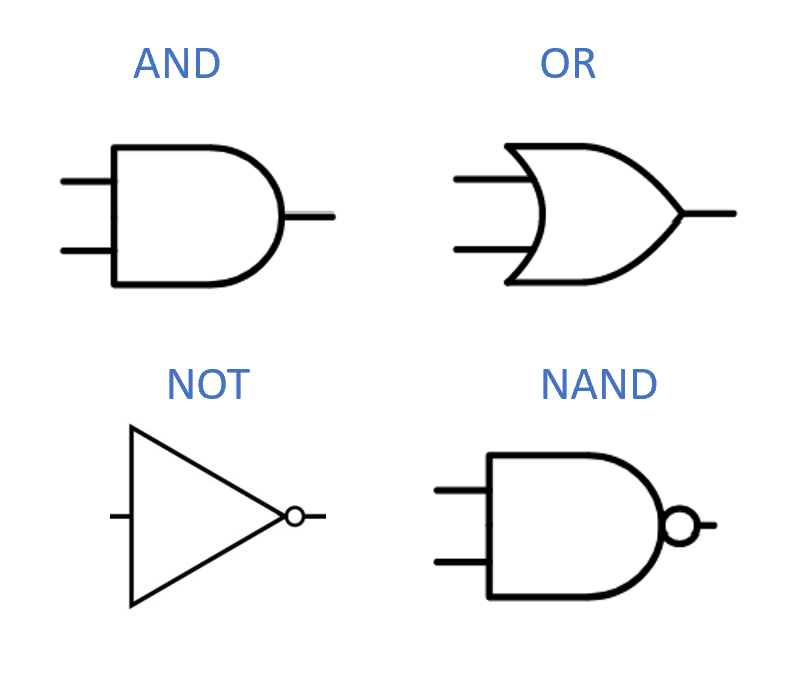
\includegraphics[width=\linewidth, height=1.5in, keepaspectratio]{../figure/logicgates.png}
\caption{Standard symbols for the logical operations or ``gates'' of
\(\ensuremath{\mathit{AND}}\), \(\ensuremath{\mathit{OR}}\),
\(\ensuremath{\mathit{NOT}}\), as well as the operation
\(\ensuremath{\mathit{NAND}}\) discussed in \cref{nandsec}.}
\label{logicgatesfig}
\end{marginfigure}


\begin{marginfigure}
\centering
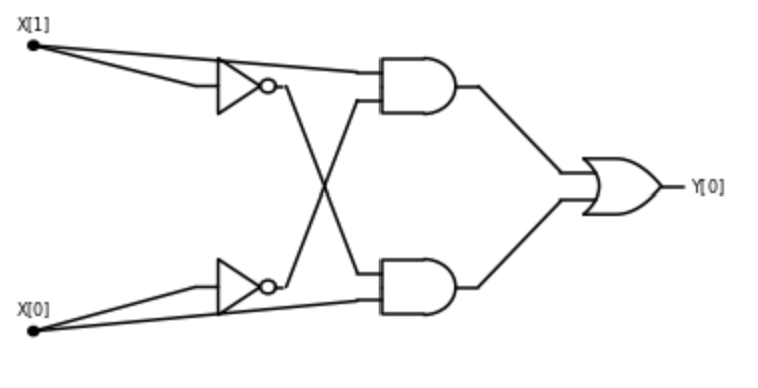
\includegraphics[width=\linewidth, height=1.5in, keepaspectratio]{../figure/xorcircuitschemdraw.png}
\caption{A circuit with \(\ensuremath{\mathit{AND}}\),
\(\ensuremath{\mathit{OR}}\) and \(\ensuremath{\mathit{NOT}}\) gates for
computing the \(\ensuremath{\mathit{XOR}}\) function.}
\label{andornotcircxorfig}
\end{marginfigure}

\emph{Boolean circuits} provide a precise notion of ``composing basic
operations together''. A Boolean circuit (see \cref{boolancircfig}) is
composed of \emph{gates} and \emph{inputs} that are connected by
\emph{wires}. The \emph{wires} carry a signal that represents either the
value \(0\) or \(1\). Each gate corresponds to either the \emph{OR},
\emph{AND}, or \emph{NOT} operation. An \emph{OR gate} has two incoming
wires, and one or more outgoing wires. If these two incoming wires carry
the signals \(a\) and \(b\) (for \(a,b \in \{0,1\}\)), then the signal
on the outgoing wires will be \(\ensuremath{\mathit{OR}}(a,b)\).
\emph{AND} and \emph{NOT} gates are defined similarly. The \emph{inputs}
have only outgoing wires. If we set a certain input to a value
\(a\in \{0,1\}\), then this value is propagated on all the wires
outgoing from it. We also designate some gates as \emph{output gates},
and their value corresponds to the result of evaluating the circuit. For
example, \cref{andornotcircxorfig} gives such a circuit for the
\(\ensuremath{\mathit{XOR}}\) function, following \cref{xoraonexample}.
We evaluate an \(n\)-input Boolean circuit \(C\) on an input
\(x\in \{0,1\}^n\) by placing the bits of \(x\) on the inputs, and then
propagating the values on the wires until we reach an output, see
\cref{boolancircfig}.

\hypertarget{booleancircimprem}{}
\begin{remark}[Physical realization of Boolean circuits] \label[remark]{booleancircimprem}

Boolean circuits are a \emph{mathematical model} that does not
necessarily correspond to a physical object, but they can be implemented
physically. In physical implementation of circuits, the signal is
\href{https://goo.gl/gntTQE}{often implemented} by electric potential,
or \emph{voltage}, on a wire, where for example voltage above a certain
level is interpreted as a logical value of \(1\), and below a certain
level is interpreted as a logical value of \(0\).
\cref{physicalimplementationsec} discusses physical implementation of
Boolean circuits (with examples including using electrical signals such
as in silicon-based circuits, but also biological and mechanical
implementations as well).

\end{remark}


\begin{figure}
\centering
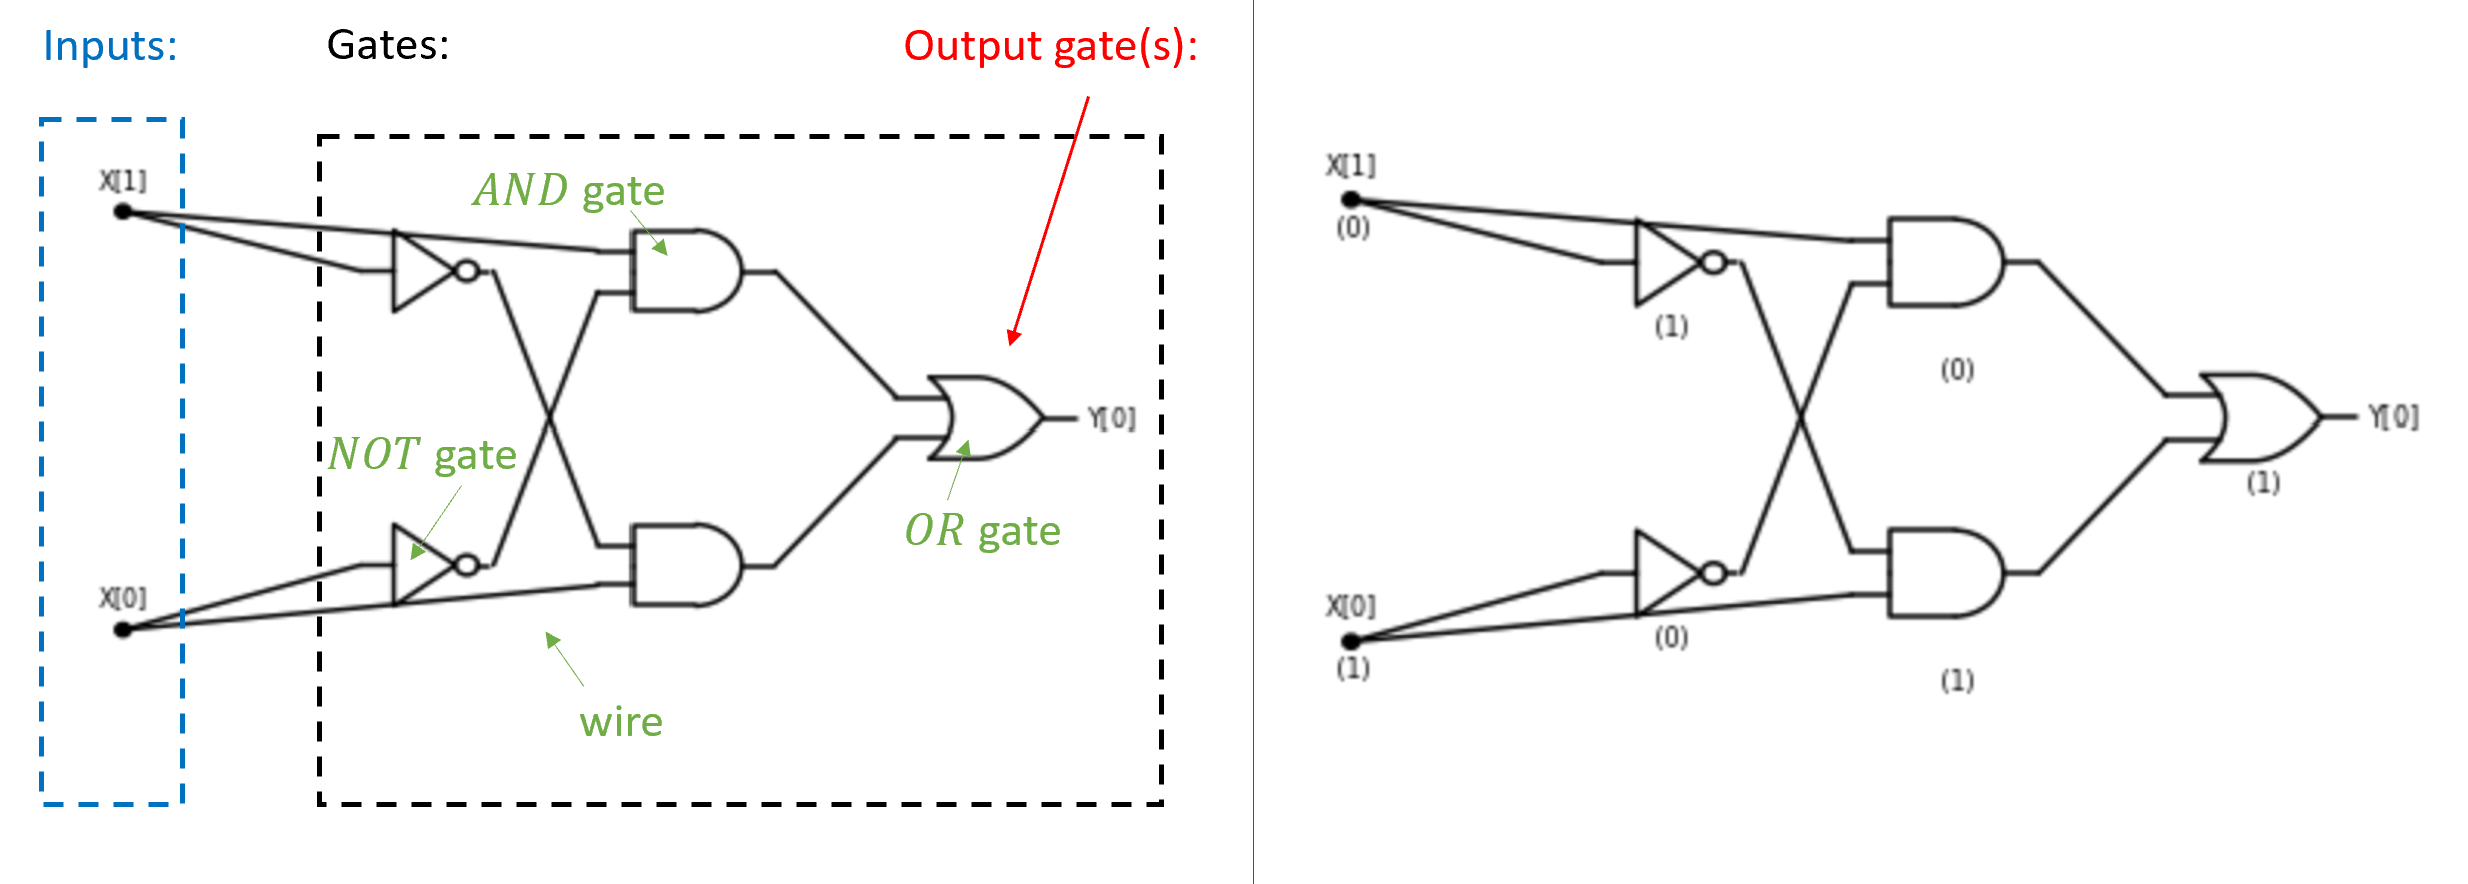
\includegraphics[width=\textwidth, height=0.25\paperheight, keepaspectratio]{../figure/booleancircuit.png}
\caption{A \emph{Boolean Circuit} consists of \emph{gates} that are
connected by \emph{wires} to one another and the \emph{inputs}. The left
side depicts a circuit with \(2\) inputs and \(5\) gates, one of which
is designated the output gate. The right side depicts the evaluation of
this circuit on the input \(x\in \{0,1\}^2\) with \(x_0=1\) and
\(x_1=0\). The value of every gate is obtained by applying the
corresponding function (\(\ensuremath{\mathit{AND}}\),
\(\ensuremath{\mathit{OR}}\), or \(\ensuremath{\mathit{NOT}}\)) to
values on the wire(s) that enter it. The output of the circuit on a
given input is the value of the output gate(s). In this case, the
circuit computes the \(\ensuremath{\mathit{XOR}}\) function and hence it
outputs \(1\) on the input \(10\).}
\label{boolancircfig}
\end{figure}

\hypertarget{allequalex}{}
\begin{solvedexercise}[All equal function] \label[solvedexercise]{allequalex}

Define \(\ensuremath{\mathit{ALLEQ}}:\{0,1\}^4 \rightarrow \{0,1\}\) to
be the function that on input \(x\in \{0,1\}^4\) outputs \(1\) if and
only if \(x_0=x_1=x_2=x_3\). Give a Boolean circuit for computing
\(\ensuremath{\mathit{ALLEQ}}\).

\end{solvedexercise}

\begin{solution} \label[solution]{Another-way-to-describe-t}

Another way to describe the function \(\ensuremath{\mathit{ALLEQ}}\) is
that it outputs \(1\) on an input \(x\in \{0,1\}^4\) if and only if
\(x = 0^4\) or \(x=1^4\). We can phrase the condition \(x=1^4\) as
\(x_0 \wedge x_1 \wedge x_2 \wedge x_3\) which can be computed using
three AND gates. Similarly we can phrase the condition \(x=0^4\) as
\(\overline{x}_0 \wedge \overline{x}_1 \wedge \overline{x}_2 \wedge \overline{x}_3\)
which can be computed using four NOT gates and three AND gates. The
output of \(\ensuremath{\mathit{ALLEQ}}\) is the OR of these two
conditions, which results in the circuit of 4 NOT gates, 6 AND gates,
and one OR gate presented in \cref{allequalfig}.

\end{solution}


\begin{marginfigure}
\centering
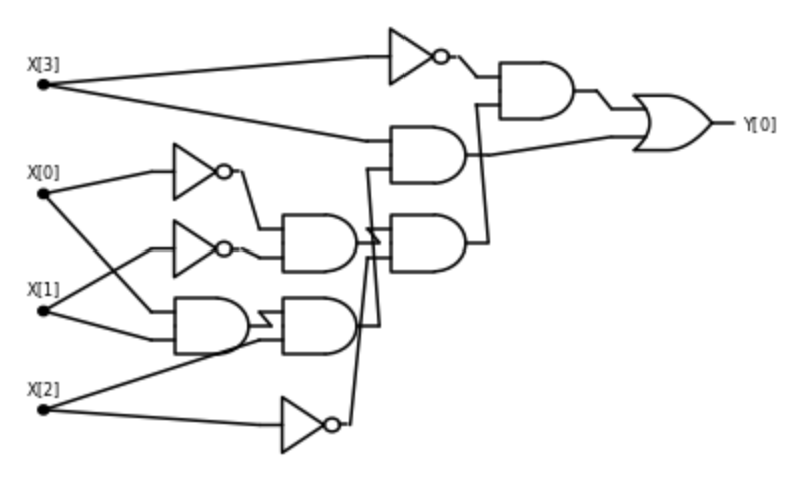
\includegraphics[width=\linewidth, height=1.5in, keepaspectratio]{../figure/allequalcirc2.png}
\caption{A Boolean circuit for computing the \emph{all equal} function
\(\ensuremath{\mathit{ALLEQ}}:\{0,1\}^4 \rightarrow \{0,1\}\) that
outputs \(1\) on \(x\in \{0,1\}^4\) if and only if \(x_0=x_1=x_2=x_3\).}
\label{allequalfig}
\end{marginfigure}

\subsection{Boolean circuits: a formal
definition}\label{Boolean-circuits-a-formal}

We defined Boolean circuits informally as obtained by connecting
\emph{AND}, \emph{OR}, and \emph{NOT} gates via wires so as to produce
an output from an input. However, to be able to prove theorems about the
existence or non-existence of Boolean circuits for computing various
functions we need to:

\begin{enumerate}
\def\labelenumi{\arabic{enumi}.}
\item
  Formally define a Boolean circuit as a mathematical object.
\item
  Formally define what it means for a circuit \(C\) to compute a
  function \(f\).
\end{enumerate}

We now proceed to do so. We will define a Boolean circuit as a labeled
\emph{Directed Acyclic Graph (DAG)}. The \emph{vertices} of the graph
correspond to the gates and inputs of the circuit, and the \emph{edges}
of the graph correspond to the wires. A wire from an input or gate \(u\)
to a gate \(v\) in the circuit corresponds to a directed edge between
the corresponding vertices. The inputs are vertices with no incoming
edges, while each gate has the appropriate number of incoming edges
based on the function it computes. (That is, \emph{AND} and \emph{OR}
gates have two in-neighbors, while \emph{NOT} gates have one
in-neighbor.) The formal definition is as follows (see also
\cref{generalcircuitfig}):


\begin{figure}
\centering
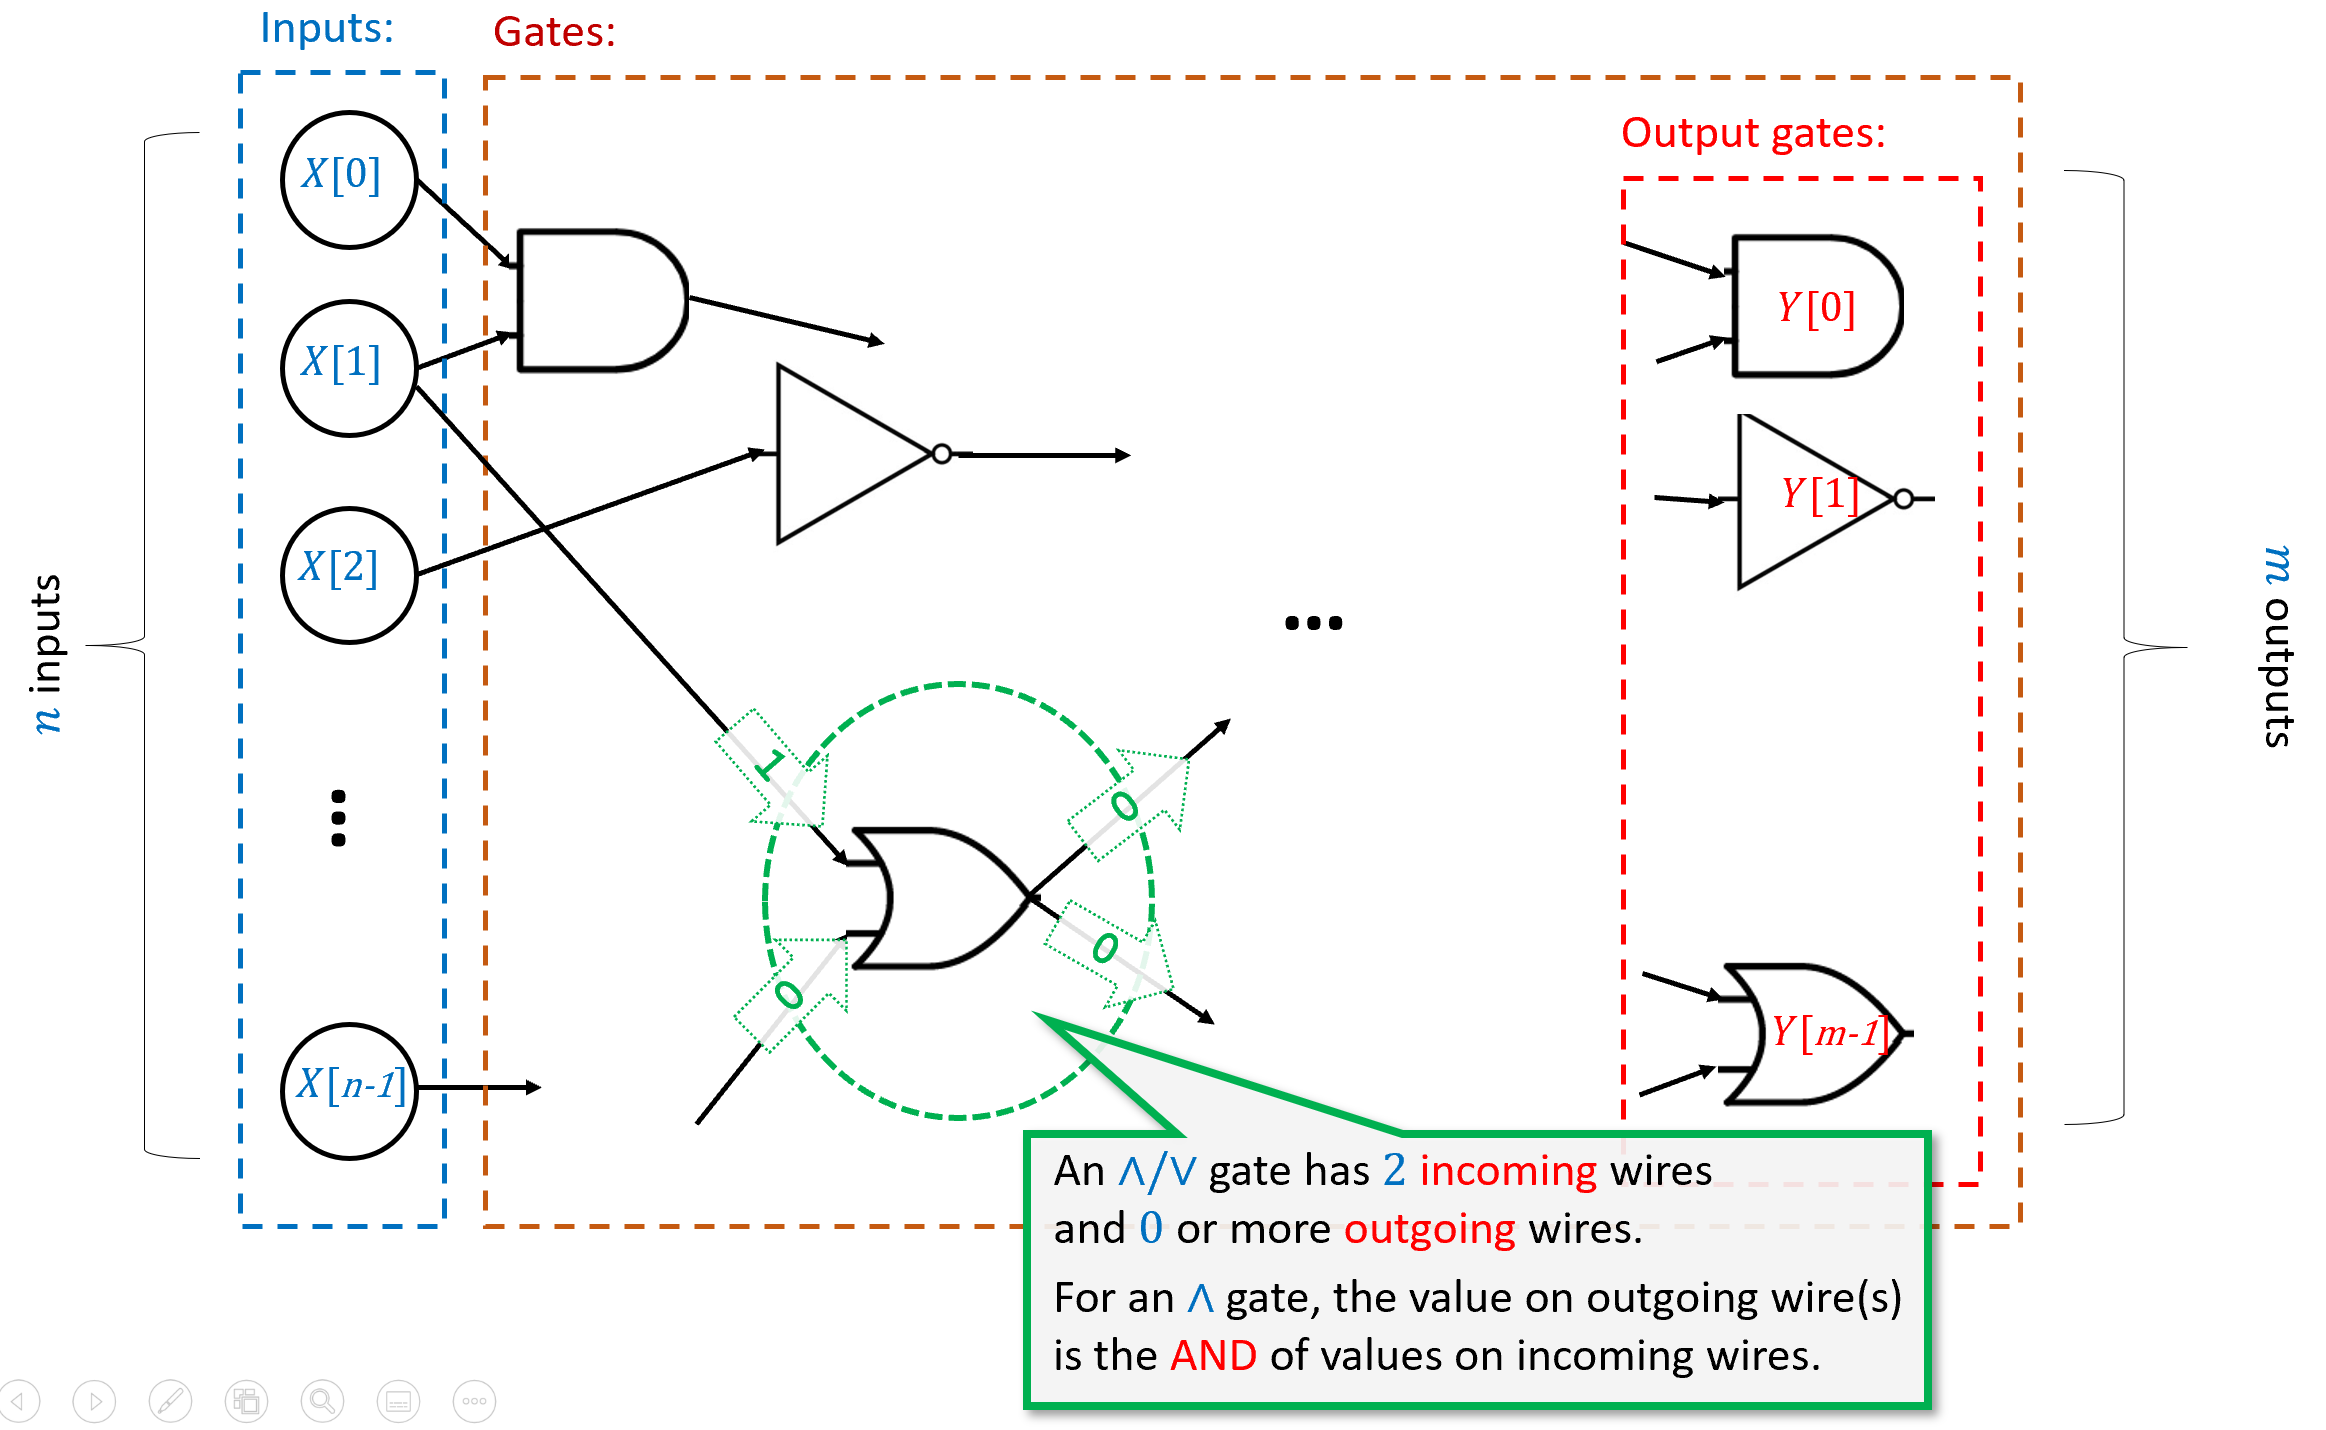
\includegraphics[width=\textwidth, height=0.25\paperheight, keepaspectratio]{../figure/generalcircuit.png}
\caption{A \emph{Boolean Circuit} is a labeled directed acyclic graph
(DAG). It has \(n\) \emph{input} vertices, which are marked with
\texttt{X[}\(0\)\texttt{]},\(\ldots\), \texttt{X[}\(n-1\)\texttt{]} and
have no incoming edges, and the rest of the vertices are \emph{gates}.
\emph{AND}, \emph{OR}, and \emph{NOT} gates have two, two, and one
incoming edges, respectively. If the circuit has \(m\) outputs, then
\(m\) of the gates are known as \emph{outputs} and are marked with
\texttt{Y[}\(0\)\texttt{]},\(\ldots\),\texttt{Y[}\(m-1\)\texttt{]}. When
we evaluate a circuit \(C\) on an input \(x\in \{0,1\}^n\), we start by
setting the value of the input vertices to \(x_0,\ldots,x_{n-1}\) and
then propagate the values, assigning to each gate \(g\) the result of
applying the operation of \(g\) to the values of \(g\)'s in-neighbors.
The output of the circuit is the value assigned to the output gates.}
\label{generalcircuitfig}
\end{figure}

\hypertarget{booleancircdef}{}
\begin{definition}[Boolean Circuits] \label[definition]{booleancircdef}

Let \(n,m,s\) be positive integers with \(s \geq m\). A \emph{Boolean
circuit} with \(n\) inputs, \(m\) outputs, and \(s\) gates, is a labeled
directed acyclic graph (DAG) \(G=(V,E)\) with \(s+n\) vertices
satisfying the following properties:

\begin{itemize}
\item
  Exactly \(n\) of the vertices have no in-neighbors. These vertices are
  known as \emph{inputs} and are labeled with the \(n\) labels
  \texttt{X[}\(0\)\texttt{]}, \(\ldots\), \texttt{X[}\(n-1\)\texttt{]}.
  Each input has at least one out-neighbor.
\item
  The other \(s\) vertices are known as \emph{gates}. Each gate is
  labeled with \(\wedge\), \(\vee\) or \(\neg\). Gates labeled with
  \(\wedge\) (\emph{AND}) or \(\vee\) (\emph{OR}) have two in-neighbors.
  Gates labeled with \(\neg\) (\emph{NOT}) have one in-neighbor. We will
  allow parallel edges.\footnote{Having parallel edges means an AND or
    OR gate \(u\) can have both its in-neighbors be the same gate \(v\).
    Since
    \(\ensuremath{\mathit{AND}}(a,a)=\ensuremath{\mathit{OR}}(a,a)=a\)
    for every \(a\in \{0,1\}\), such parallel edges don't help in
    computing new values in circuits with AND/OR/NOT gates. However, we
    will see circuits with more general sets of gates later on.}
\item
  Exactly \(m\) of the gates are also labeled with the \(m\) labels
  \texttt{Y[}\(0\)\texttt{]}, \(\ldots\), \texttt{Y[}\(m-1\)\texttt{]}
  (in addition to their label \(\wedge\)/\(\vee\)/\(\neg\)). These are
  known as \emph{outputs}.
\end{itemize}

The \emph{size} of a Boolean circuit is the number of gates it contains.

\end{definition}

\begin{pause} \label[pause]{This-is-a-non-trivial-mat}

This is a non-trivial mathematical definition, so it is worth taking the
time to read it slowly and carefully. As in all mathematical
definitions, we are using a known mathematical object --- a directed
acyclic graph (DAG) --- to define a new object, a Boolean circuit. This
might be a good time to review some of the basic properties of DAGs and
in particular the fact that they can be \emph{topologically sorted}, see
\cref{topsortsec}.

\end{pause}

If \(C\) is a circuit with \(n\) inputs and \(m\) outputs, and
\(x\in \{0,1\}^n\), then we can compute the output of \(C\) on the input
\(x\) in the natural way: assign the input vertices
\texttt{X[}\(0\)\texttt{]}, \(\ldots\), \texttt{X[}\(n-1\)\texttt{]} the
values \(x_0,\ldots,x_{n-1}\), apply each gate on the values of its
in-neighbors, and then output the values that correspond to the output
vertices. Formally, this is defined as follows:

\hypertarget{circuitcomputedef}{}
\begin{definition}[Computing a function via a Boolean circuit] \label[definition]{circuitcomputedef}

Let \(C\) be a Boolean circuit with \(n\) inputs and \(m\) outputs. For
every \(x\in \{0,1\}^n\), the \emph{output} of \(C\) on the input \(x\),
denoted by \(C(x)\), is defined as the result of the following process:

We let \(h:V \rightarrow \N\) be the \emph{minimal layering} of \(C\)
(aka \emph{topological sorting}, see \cref{minimallayeruniquethm}). We
let \(L\) be the maximum layer of \(h\), and for \(\ell=0,1,\ldots,L\)
we do the following:

\begin{itemize}
\item
  For every \(v\) in the \(\ell\)-th layer (i.e., \(v\) such that
  \(h(v)=\ell\)) do:

  \begin{itemize}
  \item
    If \(v\) is an input vertex labeled with \texttt{X[}\(i\)\texttt{]}
    for some \(i\in [n]\), then we assign to \(v\) the value \(x_i\).
  \item
    If \(v\) is a gate vertex labeled with \(\wedge\) and with two
    in-neighbors \(u,w\) then we assign to \(v\) the \emph{AND} of the
    values assigned to \(u\) and \(w\). (Since \(u\) and \(w\) are
    in-neighbors of \(v\), they are in a lower layer than \(v\), and
    hence their values have already been assigned.)
  \item
    If \(v\) is a gate vertex labeled with \(\vee\) and with two
    in-neighbors \(u,w\) then we assign to \(v\) the OR of the values
    assigned to \(u\) and \(w\).
  \item
    If \(v\) is a gate vertex labeled with \(\neg\) and with one
    in-neighbor \(u\) then we assign to \(v\) the negation of the value
    assigned to \(u\).
  \end{itemize}
\item
  The result of this process is the value \(y\in \{0,1\}^m\) such that
  for every \(j\in [m]\), \(y_j\) is the value assigned to the vertex
  with label \texttt{Y[}\(j\)\texttt{]}.
\end{itemize}

Let \(f:\{0,1\}^n \rightarrow \{0,1\}^m\). We say that the circuit \(C\)
\emph{computes} \(f\) if for every \(x\in \{0,1\}^n\), \(C(x)=f(x)\).

\end{definition}

\hypertarget{booleancircuitsremarks}{}
\begin{remark}[Boolean circuits nitpicks (optional)] \label[remark]{booleancircuitsremarks}

In phrasing \cref{booleancircdef}, we've made some technical choices
that are not very important, but will be convenient for us later on.
Having parallel edges means an AND or OR gate \(u\) can have both its
in-neighbors be the same gate \(v\). Since
\(\ensuremath{\mathit{AND}}(a,a)=\ensuremath{\mathit{OR}}(a,a)=a\) for
every \(a\in \{0,1\}\), such parallel edges don't help in computing new
values in circuits with AND/OR/NOT gates. However, we will see circuits
with more general sets of gates later on. The condition that every input
vertex has at least one out-neighbor is also not very important because
we can always add ``dummy gates'' that touch these inputs. However, it
is convenient since it guarantees that (since every gate has at most two
in-neighbors) that the number of inputs in a circuit is never larger
than twice its size.

\end{remark}

\subsection{Equivalence of circuits and straight-line
programs}\label{Equivalence-of-circuits-a}

We have seen two ways to describe how to compute a function \(f\) using
\emph{AND}, \emph{OR} and \emph{NOT}:

\begin{itemize}
\item
  A \emph{Boolean circuit}, defined in \cref{booleancircdef}, computes
  \(f\) by connecting via wires \emph{AND}, \emph{OR}, and \emph{NOT}
  gates to the inputs.
\item
  We can also describe such a computation using a \emph{straight-line
  program} that has lines of the form \texttt{foo = AND(bar,blah)},
  \texttt{foo = OR(bar,blah)} and \texttt{foo = NOT(bar)} where
  \texttt{foo}, \texttt{bar} and \texttt{blah} are variable names. (We
  call this a \emph{straight-line program} since it contains no loops or
  branching (e.g., if/then) statements.)
\end{itemize}

We now formally define the AON-CIRC programming language (``AON'' stands
for \emph{AND}/\emph{OR}/\emph{NOT}; ``CIRC'' stands for \emph{circuit})
which has the above operations, and show that it is equivalent to
Boolean circuits.

\hypertarget{AONcircdef}{}
\begin{definition}[AON-CIRC Programming language] \label[definition]{AONcircdef}

An \emph{AON-CIRC program} is a string of lines of the form
\texttt{foo = AND(bar,blah)}, \texttt{foo = OR(bar,blah)} and
\texttt{foo = NOT(bar)} where \texttt{foo}, \texttt{bar} and
\texttt{blah} are variable names.\footnote{We follow the common
  \href{https://goo.gl/QyHa3b}{programming languages convention} of
  using names such as \texttt{foo}, \texttt{bar}, \texttt{baz},
  \texttt{blah} as stand-ins for generic identifiers. A variable
  identifier in our programming language can be any combination of
  letters, numbers, underscores, and brackets. The
  \href{http://tiny.cc/introtcsappendix}{appendix} contains a full
  formal specification of our programming language.} Variables of the
form \texttt{X[}\(i\)\texttt{]} are known as \emph{input} variables, and
variables of the form \texttt{Y[}\(j\)\texttt{]} are known as
\emph{output} variables. In every line, the variables on the righthand
side of the assignment operators must either be input variables or
variables that have already been assigned a value.

A valid AON-CIRC program \(P\) includes input variables of the form
\texttt{X[}\(0\)\texttt{]},\(\ldots\),\texttt{X[}\(n-1\)\texttt{]} and
output variables of the form \texttt{Y[}\(0\)\texttt{]},\(\ldots\),
\texttt{Y[}\(m-1\)\texttt{]} for some \(n,m \geq 1\). If \(P\) is valid
AON-CIRC program and \(x\in \{0,1\}^n\), then we define the \emph{output
of \(P\) on input \(x\)}, denoted by \(P(x)\), to be the string
\(y\in \{0,1\}^m\) corresponding to the values of the output variables
\texttt{Y[}\(0\)\texttt{]} ,\(\ldots\), \texttt{Y[}\(m-1\)\texttt{]} in
the execution of \(P\) where we initialize the input variables
\texttt{X[}\(0\)\texttt{]},\(\ldots\),\texttt{X[}\(n-1\)\texttt{]} to
the values \(x_0,\ldots,x_{n-1}\).

We say that such an AON-CIRC program \(P\) \emph{computes} a function
\(f:\{0,1\}^n \rightarrow \{0,1\}^m\) if \(P(x)=f(x)\) for every
\(x\in \{0,1\}^n\).

\end{definition}

AON-CIRC is not a practical programming language: it was designed for
pedagogical purposes only, as a way to model computation as composition
of \(\ensuremath{\mathit{AND}}\), \(\ensuremath{\mathit{OR}}\), and
\(\ensuremath{\mathit{NOT}}\). However, AON-CIRC can still be easily
implemented on a computer. The following solved exercise gives an
example of an AON-CIRC program.

\hypertarget{aonforcmpsolved}{}
\begin{solvedexercise} \label[solvedexercise]{aonforcmpsolved}

Consider the following function
\(\ensuremath{\mathit{CMP}}:\{0,1\}^4 \rightarrow \{0,1\}\) that on four
input bits \(a,b,c,d\in \{0,1\}\), outputs \(1\) iff the number
represented by \((a,b)\) is larger than the number represented by
\((c,d)\). That is \(\ensuremath{\mathit{CMP}}(a,b,c,d)=1\) iff
\(2a+b>2c+d\).

Write an AON-CIRC program to compute \(\ensuremath{\mathit{CMP}}\).

\end{solvedexercise}

\begin{solution} \label[solution]{Writing-such-a-program-is}

Writing such a program is tedious but not truly hard. To compare two
numbers we first compare their most significant digit, and then go down
to the next digit and so on and so forth. In this case where the numbers
have just two binary digits, these comparisons are particularly simple.
The number represented by \((a,b)\) is larger than the number
represented by \((c,d)\) if and only if one of the following conditions
happens:

\begin{enumerate}
\def\labelenumi{\arabic{enumi}.}
\tightlist
\item
  The most significant bit \(a\) of \((a,b)\) is larger than the most
  significant bit \(c\) of \((c,d)\).
\end{enumerate}

or

\begin{enumerate}
\def\labelenumi{\arabic{enumi}.}
\setcounter{enumi}{1}
\tightlist
\item
  The two most significant bits \(a\) and \(c\) are equal, but \(b>d\).
\end{enumerate}

Another way to express the same condition is the following: the number
\((a,b)\) is larger than \((c,d)\) iff \(a>c\) \textbf{OR} (\(a\ge c\)
\textbf{AND} \(b>d\)).

For binary digits \(\alpha,\beta\), the condition \(\alpha>\beta\) is
simply that \(\alpha=1\) and \(\beta=0\) or
\(\ensuremath{\mathit{AND}}(\alpha,\ensuremath{\mathit{NOT}}(\beta))=1\),
and the condition \(\alpha\ge\beta\) is simply
\(\ensuremath{\mathit{OR}}(\alpha, \ensuremath{\mathit{NOT}}(\beta))=1\).
Together these observations can be used to give the following AON-CIRC
program to compute \(\ensuremath{\mathit{CMP}}\):

\begin{code}
temp_1 = NOT(X[2])
temp_2 = AND(X[0],temp_1)
temp_3 = OR(X[0],temp_1)
temp_4 = NOT(X[3])
temp_5 = AND(X[1],temp_4)
temp_6 = AND(temp_5,temp_3)
Y[0] = OR(temp_2,temp_6)
\end{code}

We can also present this 8-line program as a circuit with 8 gates, see
\cref{aoncmpfig}.

\end{solution}


\begin{marginfigure}
\centering
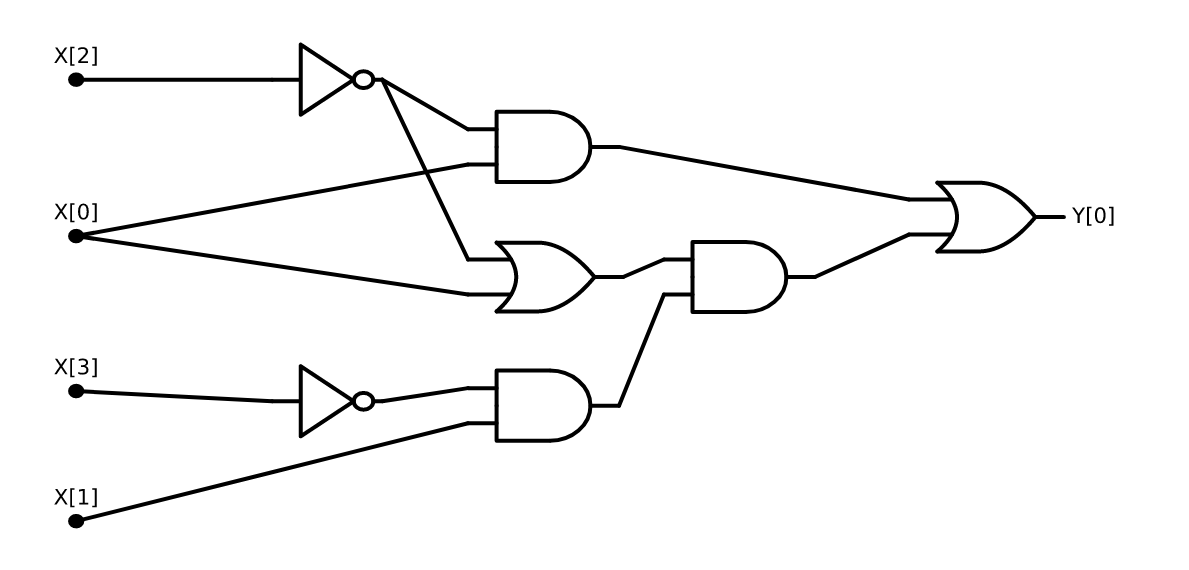
\includegraphics[width=\linewidth, height=1.5in, keepaspectratio]{../figure/comparecircuit.png}
\caption{A circuit for computing the \(\ensuremath{\mathit{CMP}}\)
function. The evaluation of this circuit on \((1,1,1,0)\) yields the
output \(1\), since the number \(3\) (represented in binary as \(11\))
is larger than the number \(2\) (represented in binary as \(10\)).}
\label{aoncmpfig}
\end{marginfigure}

It turns out that AON-CIRC programs and Boolean circuits have exactly
the same power:

\hypertarget{slcircuitequivthm}{}
\begin{theorem}[Equivalence of circuits and straight-line programs] \label[theorem]{slcircuitequivthm}

Let \(f:\{0,1\}^n \rightarrow \{0,1\}^m\) and \(s \geq m\) be some
number. Then \(f\) is computable by a Boolean circuit of \(s\) gates if
and only if \(f\) is computable by an AON-CIRC program of \(s\) lines.

\end{theorem}

\begin{proofidea} \label[proofidea]{The-idea-is-simple---AON-}

The idea is simple - AON-CIRC programs and Boolean circuits are just
different ways of describing the exact same computational process. For
example, an \emph{AND} gate in a Boolean circuit corresponding to
computing the \emph{AND} of two previously-computed values. In a
AON-CIRC program this will correspond to the line that stores in a
variable the \texttt{AND} of two previously-computed variables.

\end{proofidea}

\begin{pause} \label[pause]{This-proof-of-crefslcircu}

This proof of \cref{slcircuitequivthm} is simple at heart, but all the
details it contains can make it a little cumbersome to read. You might
be better off trying to work it out yourself before reading it. Our
\href{https://github.com/boazbk/tcscode}{GitHub repository} contains a
``proof by Python'' of \cref{slcircuitequivthm}: implementation of
functions \texttt{circuit2prog} and \texttt{prog2circuits} mapping
Boolean circuits to AON-CIRC programs and vice versa.

\end{pause}

\begin{proof}[Proof of \cref{slcircuitequivthm}] \label[proof]{Let-fn-rightarrow-m-Since}

Let \(f:\{0,1\}^n \rightarrow \{0,1\}^m\). Since the theorem is an ``if
and only if'' statement, to prove it we need to show both directions:
translating an AON-CIRC program that computes \(f\) into a circuit that
computes \(f\), and translating a circuit that computes \(f\) into an
AON-CIRC program that does so.

We start with the first direction. Let \(P\) be an \(s\) line AON-CIRC
that computes \(f\). We define a circuit \(C\) as follows: the circuit
will have \(n\) inputs and \(s\) gates. For every \(i \in [s]\), if the
\(i\)-th line has the form \texttt{foo = AND(bar,blah)} then the
\(i\)-th gate in the circuit will be an AND gate that is connected to
gates \(j\) and \(k\) where \(j\) and \(k\) correspond to the last lines
before \(i\) where the variables \texttt{bar} and \texttt{blah}
(respectively) where written to. (For example, if \(i=57\) and the last
line \texttt{bar} was written to is \(35\) and the last line
\texttt{blah} was written to is \(17\) then the two in-neighbors of gate
\(57\) will be gates \(35\) and \(17\).) If either \texttt{bar} or
\texttt{blah} is an input variable then we connect the gate to the
corresponding input vertex instead. If \texttt{foo} is an output
variable of the form \texttt{Y[}\(j\)\texttt{]} then we add the same
label to the corresponding gate to mark it as an output gate. We do the
analogous operations if the \(i\)-th line involves an \texttt{OR} or a
\texttt{NOT} operation (except that we use the corresponding \emph{OR}
or \emph{NOT} gate, and in the latter case have only one in-neighbor
instead of two). For every input \(x\in \{0,1\}^n\), if we run the
program \(P\) on \(x\), then the value written that is computed in the
\(i\)-th line is exactly the value that will be assigned to the \(i\)-th
gate if we evaluate the circuit \(C\) on \(x\). Hence \(C(x)=P(x)\) for
every \(x\in \{0,1\}^n\).

For the other direction, let \(C\) be a circuit of \(s\) gates and \(n\)
inputs that computes the function \(f\). We sort the gates according to
a topological order and write them as \(v_0,\ldots,v_{s-1}\). We now can
create a program \(P\) of \(s\) lines as follows. For every
\(i\in [s]\), if \(v_i\) is an AND gate with in-neighbors \(v_j,v_k\)
then we will add a line to \(P\) of the form \texttt{temp\_}\(i\)
\texttt{= AND(temp\_}\(j\)\texttt{,temp\_}\(k\)\texttt{)}, unless one of
the vertices is an input vertex or an output gate, in which case we
change this to the form \texttt{X[.]} or \texttt{Y[.]} appropriately.
Because we work in topological ordering, we are guaranteed that the
in-neighbors \(v_j\) and \(v_k\) correspond to variables that have
already been assigned a value. We do the same for OR and NOT gates. Once
again, one can verify that for every input \(x\), the value \(P(x)\)
will equal \(C(x)\) and hence the program computes the same function as
the circuit. (Note that since \(C\) is a valid circuit, per
\cref{booleancircdef}, every input vertex of \(C\) has at least one
out-neighbor and there are exactly \(m\) output gates labeled
\(0,\ldots,m-1\); hence all the variables \texttt{X[0]}, \(\ldots\),
\texttt{X[}\(n-1\)\texttt{]} and \texttt{Y[0]} ,\(\ldots\),
\texttt{Y[}\(m-1\)\texttt{]} will appear in the program \(P\).)

\end{proof}


\begin{marginfigure}
\centering
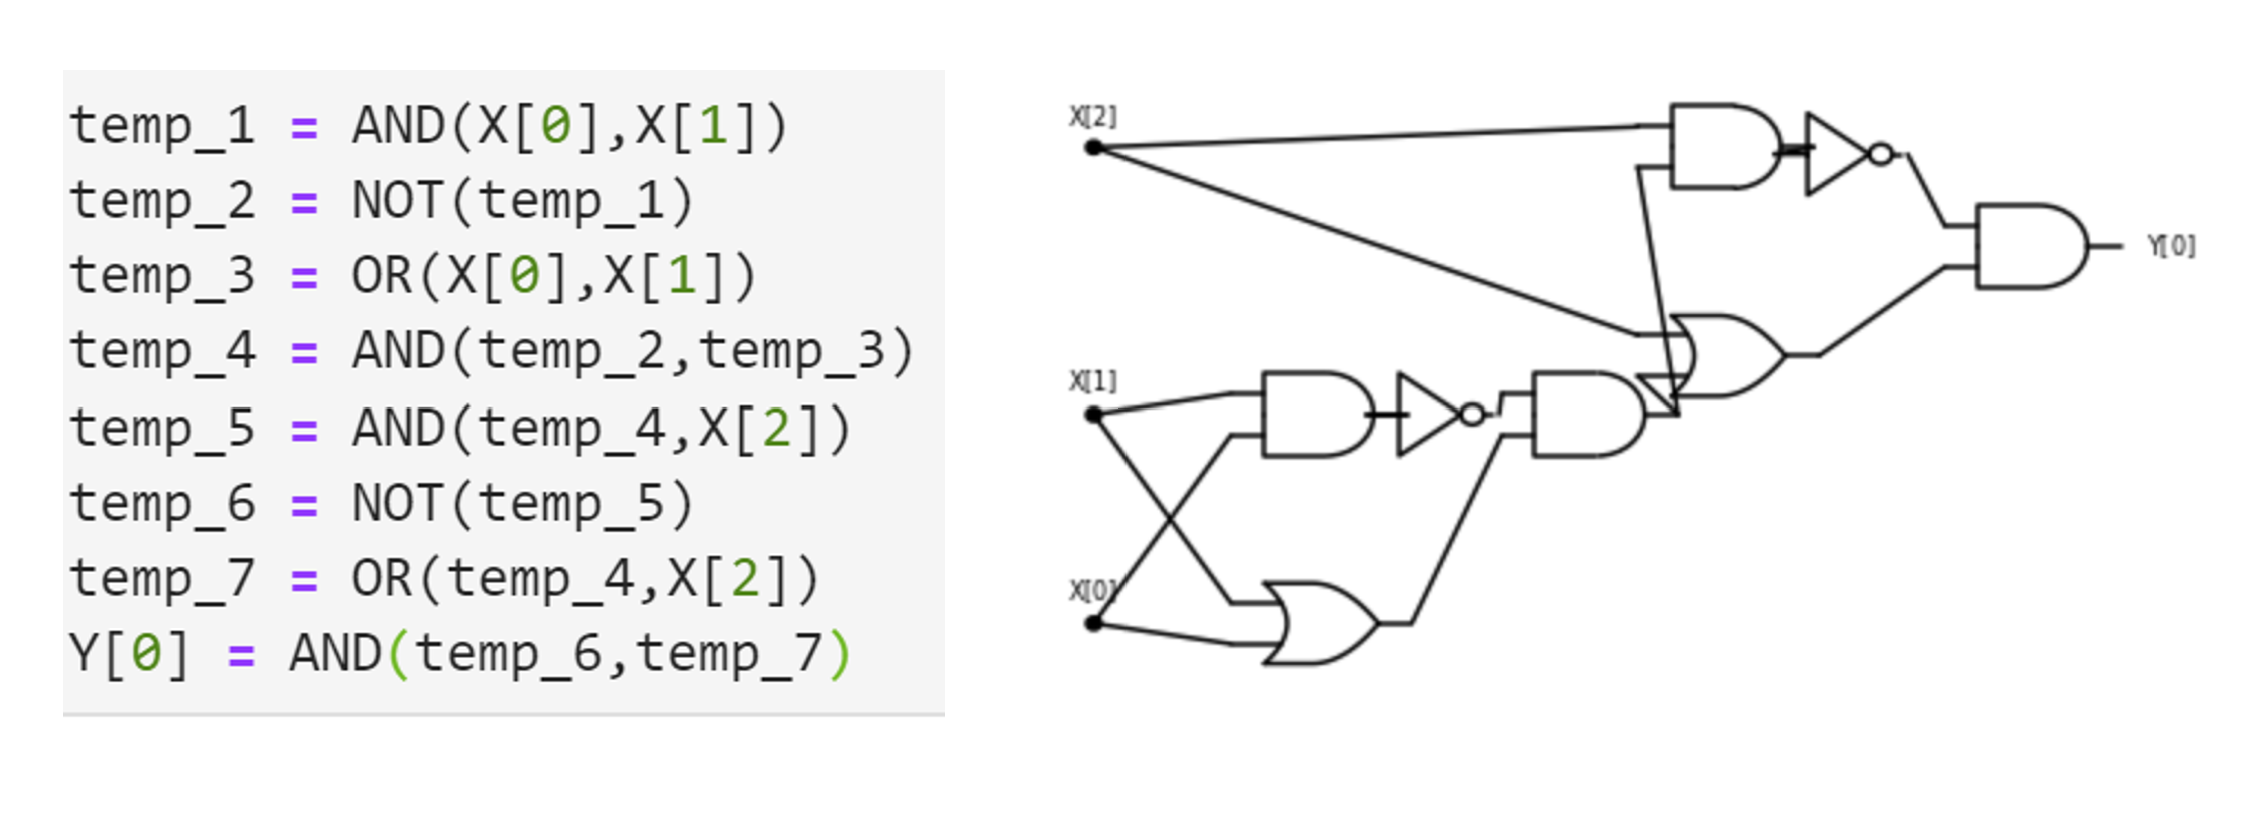
\includegraphics[width=\linewidth, height=1.5in, keepaspectratio]{../figure/aoncircequiv.png}
\caption{Two equivalent descriptions of the same AND/OR/NOT computation
as both an AON program and a Boolean circuit.}
\label{aoncircequivfig}
\end{marginfigure}

\section{Physical implementations of computing devices
(digression)}\label{physicalimplementationsec}

\emph{Computation} is an abstract notion that is distinct from its
physical \emph{implementations}. While most modern computing devices are
obtained by mapping logical gates to semiconductor based transistors,
over history people have computed using a huge variety of mechanisms,
including mechanical systems, gas and liquid (known as \emph{fluidics}),
biological and chemical processes, and even living creatures (e.g., see
\cref{crabfig} or
\href{https://www.youtube.com/watch?v=czk4xgdhdY4}{this video} for how
crabs or slime mold can be used to do computations).

In this section we will review some of these implementations, both so
you can get an appreciation of how it is possible to directly translate
Boolean circuits to the physical world, without going through the entire
stack of architecture, operating systems, and compilers, as well as to
emphasize that silicon-based processors are by no means the only way to
perform computation. Indeed, as we will see in \cref{quantumchap}, a
very exciting recent line of work involves using different media for
computation that would allow us to take advantage of \emph{quantum
mechanical effects} to enable different types of algorithms.


\begin{marginfigure}
\centering
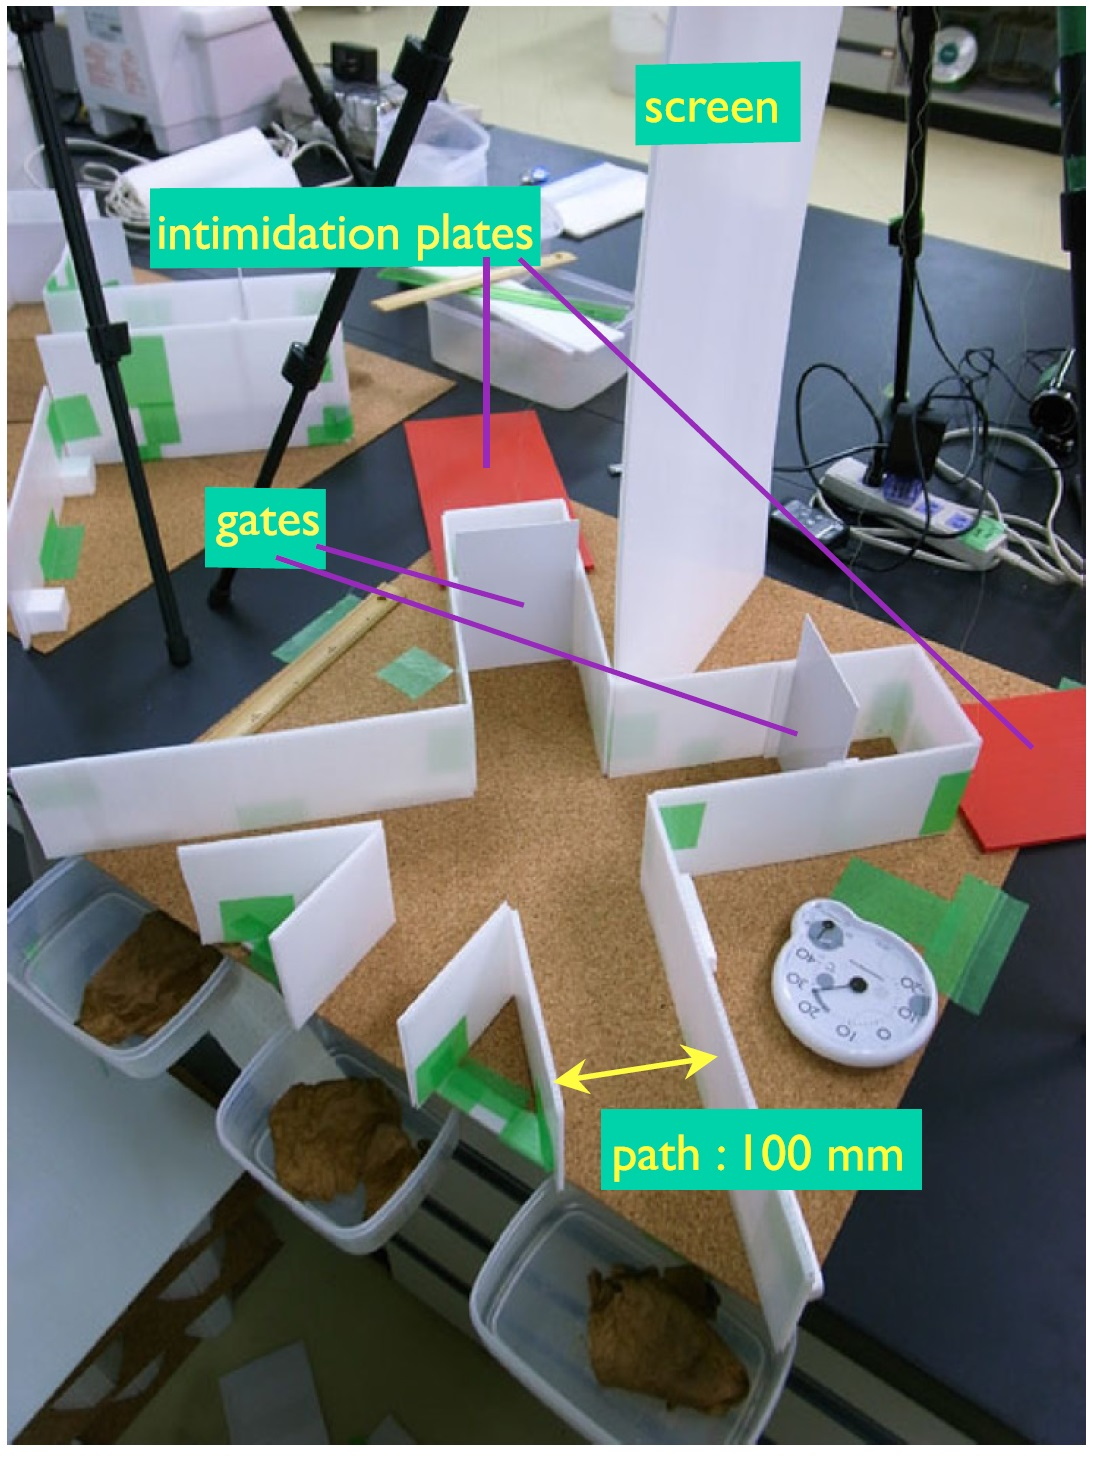
\includegraphics[width=\linewidth, height=1.5in, keepaspectratio]{../figure/crab-gate.jpg}
\caption{Crab-based logic gates from the paper ``Robust soldier-crab
ball gate'' by Gunji, Nishiyama and Adamatzky. This is an example of an
AND gate that relies on the tendency of two swarms of crabs arriving
from different directions to combine to a single swarm that continues in
the average of the directions.}
\label{crabfig}
\end{marginfigure}

\subsection{Transistors}\label{Transistors}

A \emph{transistor} can be thought of as an electric circuit with two
inputs, known as the \emph{source} and the \emph{gate} and an output,
known as the \emph{sink}. The gate controls whether current flows from
the source to the sink. In a \emph{standard transistor}, if the gate is
``ON'' then current can flow from the source to the sink and if it is
``OFF'' then it can't. In a \emph{complementary transistor} this is
reversed: if the gate is ``OFF'' then current can flow from the source
to the sink and if it is ``ON'' then it can't.


\begin{marginfigure}
\centering
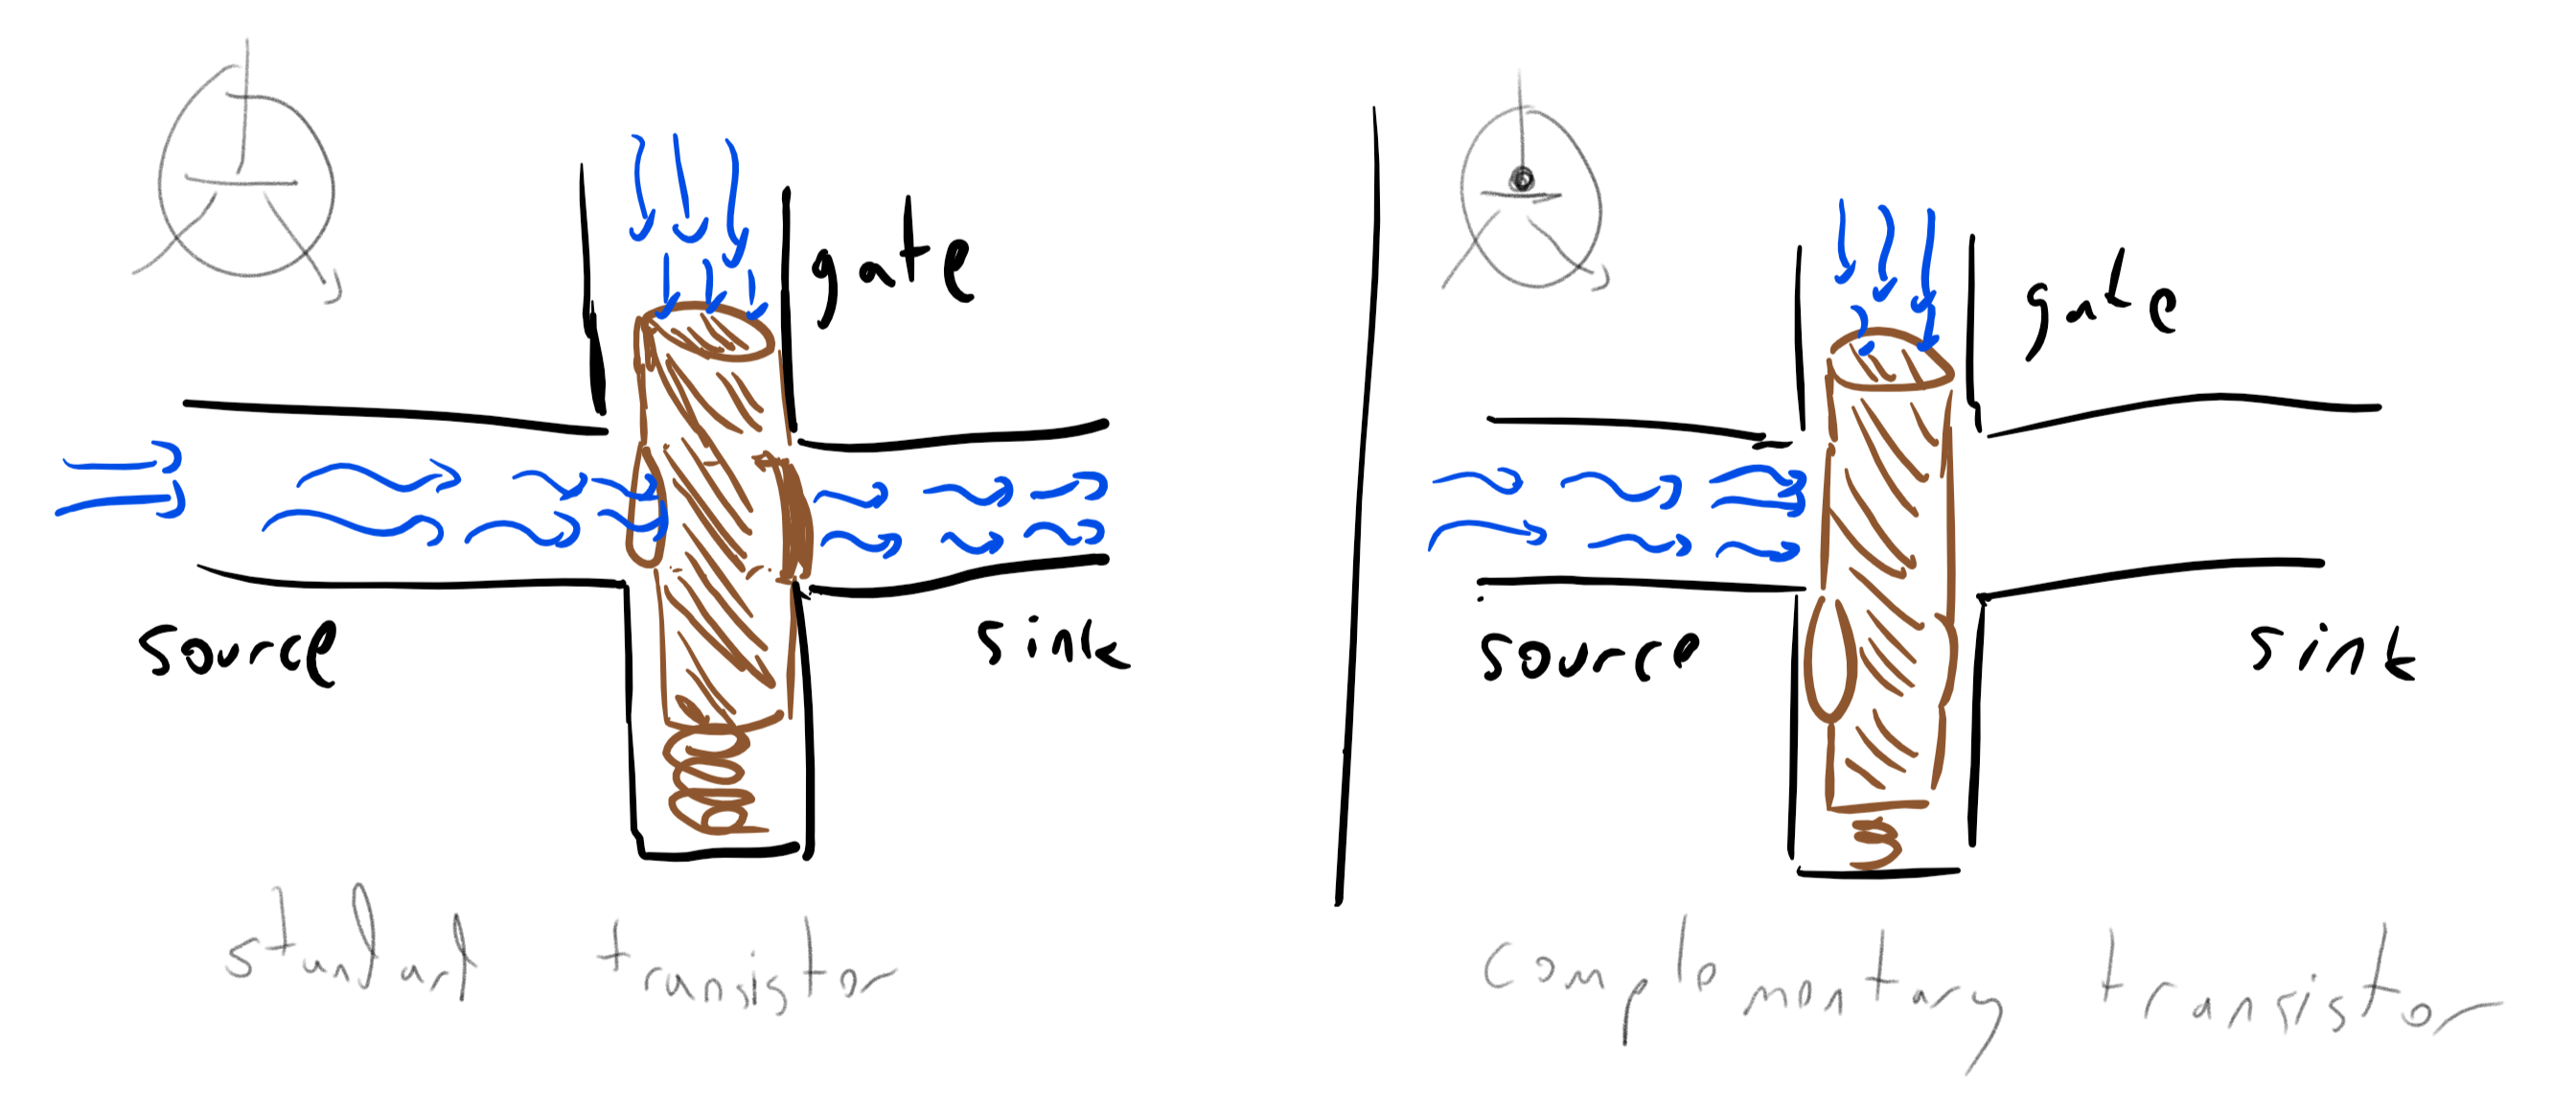
\includegraphics[width=\linewidth, height=1.5in, keepaspectratio]{../figure/transistor_water.png}
\caption{We can implement the logic of transistors using water. The
water pressure from the gate closes or opens a faucet between the source
and the sink.}
\label{transistor-water-fig}
\end{marginfigure}

There are several ways to implement the logic of a transistor. For
example, we can use faucets to implement it using water pressure
(e.g.~\cref{transistor-water-fig}). This might seem as merely a
curiosity, but there is a field known as
\href{https://en.wikipedia.org/wiki/Fluidics}{fluidics} concerned with
implementing logical operations using liquids or gasses. Some of the
motivations include operating in extreme environmental conditions such
as in space or a battlefield, where standard electronic equipment would
not survive.

The standard implementations of transistors use electrical current. One
of the original implementations used \emph{vacuum tubes}. As its name
implies, a vacuum tube is a tube containing nothing (i.e., a vacuum) and
where a priori electrons could freely flow from the source (a wire) to
the sink (a plate). However, there is a gate (a grid) between the two,
where modulating its voltage can block the flow of electrons.

Early vacuum tubes were roughly the size of lightbulbs (and looked very
much like them too). In the 1950's they were supplanted by
\emph{transistors}, which implement the same logic using
\emph{semiconductors} which are materials that normally do not conduct
electricity but whose conductivity can be modified and controlled by
inserting impurities (``doping'') and applying an external electric
field (this is known as the \emph{field effect}). In the 1960's
computers started to be implemented using \emph{integrated circuits}
which enabled much greater density. In 1965, Gordon Moore predicted that
the number of transistors per integrated circuit would double every year
(see \cref{moorefig}), and that this would lead to ``such wonders as
home computers ---or at least terminals connected to a central
computer--- automatic controls for automobiles, and personal portable
communications equipment''. Since then, (adjusted versions of) this
so-called ``Moore's law'' have been running strong, though exponential
growth cannot be sustained forever, and some physical limitations are
already
\href{http://www.nature.com/news/the-chips-are-down-for-moore-s-law-1.19338}{becoming
apparent}.


\begin{marginfigure}
\centering
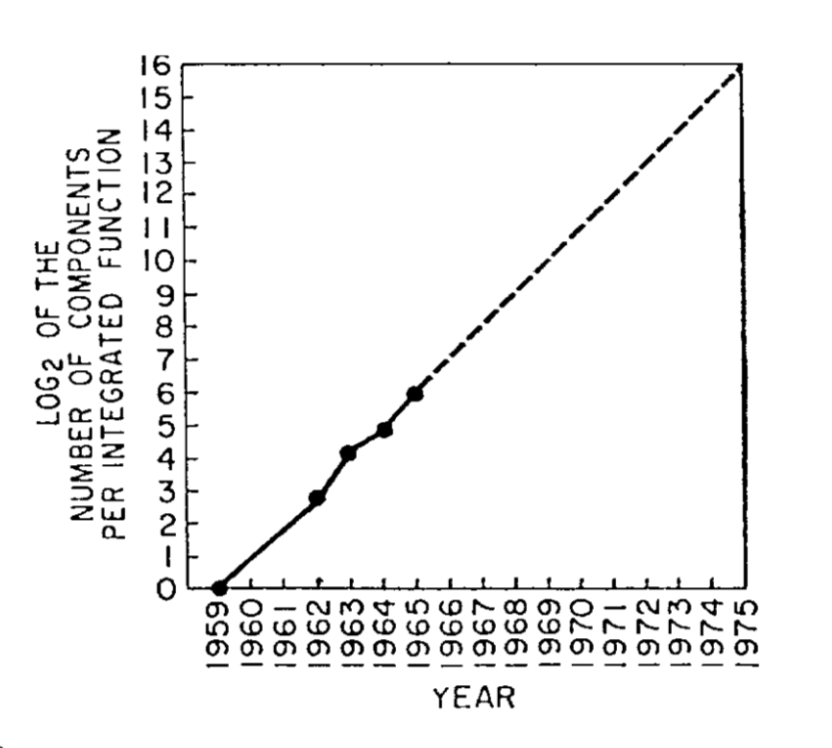
\includegraphics[width=\linewidth, height=1.5in, keepaspectratio]{../figure/gordon_moore.png}
\caption{The number of transistors per integrated circuits from 1959
till 1965 and a prediction that exponential growth will continue for at
least another decade. Figure taken from ``Cramming More Components onto
Integrated Circuits'', Gordon Moore, 1965}
\label{moorefig}
\end{marginfigure}


\begin{marginfigure}
\centering
\includegraphics[width=\linewidth, height=1.5in, keepaspectratio]{../figure/moore_cartoon.png}
\caption{Cartoon from Gordon Moore's article ``predicting'' the
implications of radically improving transistor density.}
\label{moore-cartoon-fig}
\end{marginfigure}


\begin{marginfigure}
\centering
\includegraphics[width=\linewidth, height=1.5in, keepaspectratio]{../figure/1200px-Moore's_Law_over_120_Years.png}
\caption{The exponential growth in computing power over the last 120
years. Graph by Steve Jurvetson, extending a prior graph of Ray
Kurzweil.}
\label{kurzweil-fig}
\end{marginfigure}

\subsection{Logical gates from
transistors}\label{Logical-gates-from-transi}

We can use transistors to implement various Boolean functions such as
\(\ensuremath{\mathit{AND}}\), \(\ensuremath{\mathit{OR}}\), and
\(\ensuremath{\mathit{NOT}}\). For each a two-input gate
\(G:\{0,1\}^2 \rightarrow \{0,1\}\), such an implementation would be a
system with two input wires \(x,y\) and one output wire \(z\), such that
if we identify high voltage with ``\(1\)'' and low voltage with
``\(0\)'', then the wire \(z\) will equal to ``\(1\)'' if and only if
applying \(G\) to the values of the wires \(x\) and \(y\) is \(1\) (see
\cref{logicgatestransistorsfig} and \cref{transistor-nand-fig}). This
means that if there exists a AND/OR/NOT circuit to compute a function
\(g:\{0,1\}^n \rightarrow \{0,1\}^m\), then we can compute \(g\) in the
physical world using transistors as well.


\begin{marginfigure}
\centering
\includegraphics[width=\linewidth, height=1.5in, keepaspectratio]{../figure/DTLLogic.PNG}
\caption{Implementing logical gates using transistors. Figure taken from
\href{http://www.northdownfarm.co.uk/rory/tim/basiclogic.htm}{Rory
Mangles' website}.}
\label{logicgatestransistorsfig}
\end{marginfigure}


\begin{marginfigure}
\centering
\includegraphics[width=\linewidth, height=1.5in, keepaspectratio]{../figure/nand_transistor.png}
\caption{Implementing a NAND gate (see \cref{nandsec}) using
transistors.}
\label{transistor-nand-fig}
\end{marginfigure}

\subsection{Biological computing}\label{Biological-computing}

Computation can be based on
\href{http://www.nature.com/nrg/journal/v13/n7/full/nrg3197.html}{biological
or chemical systems}. For example the
\href{https://en.wikipedia.org/wiki/Lac_operon}{\emph{lac} operon}
produces the enzymes needed to digest lactose only if the conditions
\(x \wedge (\neg y)\) hold where \(x\) is ``lactose is present'' and
\(y\) is ``glucose is present''. Researchers have managed to
\href{http://science.sciencemag.org/content/340/6132/554?iss=6132}{create
transistors}, and from them logic gates, based on DNA molecules (see
also \cref{transcriptorfig}). One motivation for DNA computing is to
achieve increased parallelism or storage density; another is to create
``smart biological agents'' that could perhaps be injected into bodies,
replicate themselves, and fix or kill cells that were damaged by a
disease such as cancer. Computing in biological systems is not
restricted, of course, to DNA: even larger systems such as
\href{https://www.cs.princeton.edu/~chazelle/pubs/cacm12-natalg.pdf}{flocks
of birds} can be considered as computational processes.


\begin{marginfigure}
\centering
\includegraphics[width=\linewidth, height=1.5in, keepaspectratio]{../figure/transcriptor.jpg}
\caption{Performance of DNA-based logic gates. Figure taken from paper
of
\href{http://science.sciencemag.org/content/early/2013/03/27/science.1232758.full}{Bonnet
et al}, Science, 2013.}
\label{transcriptorfig}
\end{marginfigure}

\subsection{Cellular automata and the game of
life}\label{Cellular-automata-and-the}

\emph{Cellular automata} is a model of a system composed of a sequence
of \emph{cells}, each of which can have a finite state. At each step, a
cell updates its state based on the states of its \emph{neighboring
cells} and some simple rules. As we will discuss later in this book (see
\cref{cellularautomatasec}), cellular automata such as Conway's ``Game
of Life'' can be used to simulate computation gates .


\begin{marginfigure}
\centering
\includegraphics[width=\linewidth, height=1.5in, keepaspectratio]{../figure/game_of_life_and.png}
\caption{An AND gate using a ``Game of Life'' configuration. Figure
taken from
\href{http://www.rennard.org/alife/CollisionBasedRennard.pdf}{Jean-Philippe
Rennard's paper}.}
\label{gameoflifefig}
\end{marginfigure}

\subsection{Neural networks}\label{Neural-networks}

One computation device that we all carry with us is our own
\emph{brain}. Brains have served humanity throughout history, doing
computations that range from distinguishing prey from predators, through
making scientific discoveries and artistic masterpieces, to composing
witty 280 character messages. The exact working of the brain is still
not fully understood, but one common mathematical model for it is a
(very large) \emph{neural network}.

A neural network can be thought of as a Boolean circuit that instead of
\(\ensuremath{\mathit{AND}}\)/\(\ensuremath{\mathit{OR}}\)/\(\ensuremath{\mathit{NOT}}\)
uses some other gates as the basic basis. For example, one particular
basis we can use are \emph{threshold gates}. For every vector
\(w= (w_0,\ldots,w_{k-1})\) of integers and integer \(t\) (some or all
of which could be negative), the \emph{threshold function corresponding
to \(w,t\)} is the function \(T_{w,t}:\{0,1\}^k \rightarrow \{0,1\}\)
that maps \(x\in \{0,1\}^k\) to \(1\) if and only if
\(\sum_{i=0}^{k-1} w_i x_i \geq t\). For example, the threshold function
\(T_{w,t}\) corresponding to \(w=(1,1,1,1,1)\) and \(t=3\) is simply the
majority function \(\ensuremath{\mathit{MAJ}}_5\) on \(\{0,1\}^5\).
Threshold gates can be thought of as an approximation for \emph{neuron
cells} that make up the core of human and animal brains. To a first
approximation, a neuron has \(k\) inputs and a single output, and the
neurons ``fires'' or ``turns on'' its output when those signals pass
some threshold.

Many machine learning algorithms use \emph{artificial neural networks}
whose purpose is not to imitate biology but rather to perform some
computational tasks, and hence are not restricted to threshold or other
biologically-inspired gates. Generally, a neural network is often
described as operating on signals that are real numbers, rather than
\(0/1\) values, and where the output of a gate on inputs
\(x_0,\ldots,x_{k-1}\) is obtained by applying \(f(\sum_i w_i x_i)\)
where \(f:\R \rightarrow \R\) is an
\href{https://goo.gl/p9izfA}{activation function} such as rectified
linear unit (ReLU), Sigmoid, or many others (see
\cref{activationfunctionsfig}). However, for the purposes of our
discussion, all of the above are equivalent (see also
\cref{NANDsfromActivationfunctionex}). In particular we can reduce the
setting of real inputs to binary inputs by representing a real number in
the binary basis, and multiplying the weight of the bit corresponding to
the \(i^{th}\) digit by \(2^i\).


\begin{marginfigure}
\centering
\includegraphics[width=\linewidth, height=1.5in, keepaspectratio]{../figure/activationfuncs.png}
\caption{Common activation functions used in Neural Networks, including
rectified linear units (ReLU), sigmoids, and hyperbolic tangent. All of
those can be thought of as continuous approximations to simple the step
function. All of these can be used to compute the NAND gate (see
\cref{NANDsfromActivationfunctionex}). This property enables neural
networks to (approximately) compute any function that can be computed by
a Boolean circuit.}
\label{activationfunctionsfig}
\end{marginfigure}

\subsection{A computer made from marbles and
pipes}\label{A-computer-made-from-marb}

We can implement computation using many other physical media, without
any electronic, biological, or chemical components. Many suggestions for
\emph{mechanical} computers have been put forward, going back at least
to Gottfried Leibniz' computing machines from the 1670s and Charles
Babbage's 1837 plan for a mechanical
\href{https://en.wikipedia.org/wiki/Analytical_Engine}{``Analytical
Engine''}. As one example, \cref{marblefig} shows a simple
implementation of a NAND (negation of AND, see \cref{nandsec}) gate
using marbles going through pipes. We represent a logical value in
\(\{0,1\}\) by a pair of pipes, such that there is a marble flowing
through exactly one of the pipes. We call one of the pipes the ``\(0\)
pipe'' and the other the ``\(1\) pipe'', and so the identity of the pipe
containing the marble determines the logical value. A NAND gate
corresponds to a mechanical object with two pairs of incoming pipes and
one pair of outgoing pipes, such that for every \(a,b \in \{0,1\}\), if
two marbles are rolling toward the object in the \(a\) pipe of the first
pair and the \(b\) pipe of the second pair, then a marble will roll out
of the object in the \(\ensuremath{\mathit{NAND}}(a,b)\)-pipe of the
outgoing pair. In fact, there is even a commercially-available
educational game that uses marbles as a basis of computing, see
\cref{turingtumblefig}.


\begin{marginfigure}
\centering
\includegraphics[width=\linewidth, height=1.5in, keepaspectratio]{../figure/marble.png}
\caption{A physical implementation of a NAND gate using marbles. Each
wire in a Boolean circuit is modeled by a pair of pipes representing the
values \(0\) and \(1\) respectively, and hence a gate has four input
pipes (two for each logical input) and two output pipes. If one of the
input pipes representing the value \(0\) has a marble in it then that
marble will flow to the output pipe representing the value \(1\). (The
dashed line represents a gadget that will ensure that at most one marble
is allowed to flow onward in the pipe.) If both the input pipes
representing the value \(1\) have marbles in them, then the first marble
will be stuck but the second one will flow onwards to the output pipe
representing the value \(0\).}
\label{marblefig}
\end{marginfigure}


\begin{marginfigure}
\centering
\includegraphics[width=\linewidth, height=1.5in, keepaspectratio]{../figure/gadget.png}
\caption{A ``gadget'' in a pipe that ensures that at most one marble can
pass through it. The first marble that passes causes the barrier to lift
and block new ones.}
\label{gadgetfig}
\end{marginfigure}


\begin{marginfigure}
\centering
\includegraphics[width=\linewidth, height=1.5in, keepaspectratio]{../figure/turingtumble.png}
\caption{The game \href{https://www.turingtumble.com/}{``Turing
Tumble''} contains an implementation of logical gates using marbles.}
\label{turingtumblefig}
\end{marginfigure}

\section{The NAND function}\label{nandsec}

The \(\ensuremath{\mathit{NAND}}\) function is another simple function
that is extremely useful for defining computation. It is the function
mapping \(\{0,1\}^2\) to \(\{0,1\}\) defined by:

\[\ensuremath{\mathit{NAND}}(a,b) = \begin{cases} 0 & a=b=1 \\ 1 & \text{otherwise} \end{cases}\;.\]

As its name implies, \(\ensuremath{\mathit{NAND}}\) is the NOT of AND
(i.e.,
\(\ensuremath{\mathit{NAND}}(a,b)= \ensuremath{\mathit{NOT}}(\ensuremath{\mathit{AND}}(a,b))\)),
and so we can clearly compute \(\ensuremath{\mathit{NAND}}\) using
\(\ensuremath{\mathit{AND}}\) and \(\ensuremath{\mathit{NOT}}\).
Interestingly, the opposite direction holds as well:

\hypertarget{univnandonethm}{}
\begin{theorem}[NAND computes AND,OR,NOT] \label[theorem]{univnandonethm}

We can compute \(\ensuremath{\mathit{AND}}\),
\(\ensuremath{\mathit{OR}}\), and \(\ensuremath{\mathit{NOT}}\) by
composing only the \(\ensuremath{\mathit{NAND}}\) function.

\end{theorem}

\begin{proof} \label[proof]{We-start-with-the-followi}

We start with the following observation. For every \(a\in \{0,1\}\),
\(\ensuremath{\mathit{AND}}(a,a)=a\). Hence,
\(\ensuremath{\mathit{NAND}}(a,a)=\ensuremath{\mathit{NOT}}(\ensuremath{\mathit{AND}}(a,a))=\ensuremath{\mathit{NOT}}(a)\).
This means that \(\ensuremath{\mathit{NAND}}\) can compute
\(\ensuremath{\mathit{NOT}}\). By the principle of ``double negation'',
\(\ensuremath{\mathit{AND}}(a,b)=\ensuremath{\mathit{NOT}}(\ensuremath{\mathit{NOT}}(\ensuremath{\mathit{AND}}(a,b)))\),
and hence we can use \(\ensuremath{\mathit{NAND}}\) to compute
\(\ensuremath{\mathit{AND}}\) as well. Once we can compute
\(\ensuremath{\mathit{AND}}\) and \(\ensuremath{\mathit{NOT}}\), we can
compute \(\ensuremath{\mathit{OR}}\) using
\href{https://goo.gl/TH86dH}{``De Morgan's Law''}:
\(\ensuremath{\mathit{OR}}(a,b)=\ensuremath{\mathit{NOT}}(\ensuremath{\mathit{AND}}(\ensuremath{\mathit{NOT}}(a),\ensuremath{\mathit{NOT}}(b)))\)
(which can also be written as
\(a \vee b = \overline{\overline{a} \wedge \overline{b}}\)) for every
\(a,b \in \{0,1\}\).

\end{proof}

\begin{pause} \label[pause]{crefunivnandonethms-proof}

\cref{univnandonethm}'s proof is very simple, but you should make sure
that \textbf{(i)} you understand the statement of the theorem, and
\textbf{(ii)} you follow its proof. In particular, you should make sure
you understand why De Morgan's law is true.

\end{pause}

We can use \(\ensuremath{\mathit{NAND}}\) to compute many other
functions, as demonstrated in the following exercise.

\hypertarget{majbynandex}{}
\begin{solvedexercise}[Compute majority with NAND] \label[solvedexercise]{majbynandex}

Let \(\ensuremath{\mathit{MAJ}}: \{0,1\}^3 \rightarrow \{0,1\}\) be the
function that on input \(a,b,c\) outputs \(1\) iff \(a+b+c \geq 2\).
Show how to compute \(\ensuremath{\mathit{MAJ}}\) using a composition of
\(\ensuremath{\mathit{NAND}}\)'s.

\end{solvedexercise}

\begin{solution} \label[solution]{Recall-that-eqrefeqmajand}

Recall that \eqref{eqmajandornot} states that

\[
\ensuremath{\mathit{MAJ}}(x_0,x_1,x_2) = \ensuremath{\mathit{OR}}\left(\, \ensuremath{\mathit{AND}}(x_0,x_1)\;,\; \ensuremath{\mathit{OR}} \bigl( \ensuremath{\mathit{AND}}(x_1,x_2) \;,\; \ensuremath{\mathit{AND}}(x_0,x_2) \bigr) \, \right) \;. \label{eqmajandornotrestated}
\]

We can use \cref{univnandonethm} to replace all the occurrences of
\(\ensuremath{\mathit{AND}}\) and \(\ensuremath{\mathit{OR}}\) with
\(\ensuremath{\mathit{NAND}}\)'s. Specifically, we can use the
equivalence
\(\ensuremath{\mathit{AND}}(a,b)=\ensuremath{\mathit{NOT}}(\ensuremath{\mathit{NAND}}(a,b))\),
\(\ensuremath{\mathit{OR}}(a,b)=\ensuremath{\mathit{NAND}}(\ensuremath{\mathit{NOT}}(a),\ensuremath{\mathit{NOT}}(b))\),
and \(\ensuremath{\mathit{NOT}}(a)=\ensuremath{\mathit{NAND}}(a,a)\) to
replace the righthand side of \eqref{eqmajandornotrestated} with an
expression involving only \(\ensuremath{\mathit{NAND}}\), yielding that
\(\ensuremath{\mathit{MAJ}}(a,b,c)\) is equivalent to the (somewhat
unwieldy) expression

\[
\begin{gathered}
\ensuremath{\mathit{NAND}} \biggl(\, \ensuremath{\mathit{NAND}}\Bigl(\, \ensuremath{\mathit{NAND}}\bigl(\ensuremath{\mathit{NAND}}(a,b),\ensuremath{\mathit{NAND}}(a,c)\bigr), \\
\ensuremath{\mathit{NAND}}\bigl(\ensuremath{\mathit{NAND}}(a,b),\ensuremath{\mathit{NAND}}(a,c)\bigr)\, \Bigr),\\
\ensuremath{\mathit{NAND}}(b,c) \, \biggr)
\end{gathered}
\]

The same formula can also be expressed as a circuit with NAND gates, see
\cref{majnandcircfig}.

\end{solution}


\begin{marginfigure}
\centering
\includegraphics[width=\linewidth, height=1.5in, keepaspectratio]{../figure/majfromnand.png}
\caption{A circuit with NAND gates to compute the Majority function on
three bits}
\label{majnandcircfig}
\end{marginfigure}

\subsection{NAND Circuits}\label{NAND-Circuits}

We define \emph{NAND Circuits} as circuits in which all the gates are
NAND operations. Such a circuit again corresponds to a directed acyclic
graph (DAG) since all the gates correspond to the same function (i.e.,
NAND), we do not even need to label them, and all gates have in-degree
exactly two. Despite their simplicity, NAND circuits can be quite
powerful.

\hypertarget{xornandexample}{}
\begin{example}[$NAND$ circuit for $XOR$] \label[example]{xornandexample}

Recall the \(\ensuremath{\mathit{XOR}}\) function which maps
\(x_0,x_1 \in \{0,1\}\) to \(x_0 + x_1 \mod 2\). We have seen in
\cref{xoraonexample} that we can compute \(\ensuremath{\mathit{XOR}}\)
using \(\ensuremath{\mathit{AND}}\), \(\ensuremath{\mathit{OR}}\), and
\(\ensuremath{\mathit{NOT}}\), and so by \cref{univnandonethm} we can
compute it using only \(\ensuremath{\mathit{NAND}}\)'s. However, the
following is a direct construction of computing
\(\ensuremath{\mathit{XOR}}\) by a sequence of NAND operations:

\begin{enumerate}
\def\labelenumi{\arabic{enumi}.}
\tightlist
\item
  Let \(u = \ensuremath{\mathit{NAND}}(x_0,x_1)\).
\item
  Let \(v = \ensuremath{\mathit{NAND}}(x_0,u)\)
\item
  Let \(w = \ensuremath{\mathit{NAND}}(x_1,u)\).
\item
  The \(\ensuremath{\mathit{XOR}}\) of \(x_0\) and \(x_1\) is
  \(y_0 = \ensuremath{\mathit{NAND}}(v,w)\).
\end{enumerate}

One can verify that this algorithm does indeed compute
\(\ensuremath{\mathit{XOR}}\) by enumerating all the four choices for
\(x_0,x_1 \in \{0,1\}\). We can also represent this algorithm
graphically as a circuit, see \cref{cornandcircfig}.

\end{example}


\begin{marginfigure}
\centering
\includegraphics[width=\linewidth, height=1.5in, keepaspectratio]{../figure/nandcircxor.png}
\caption{A circuit with NAND gates to compute the XOR of two bits.}
\label{cornandcircfig}
\end{marginfigure}

In fact, we can show the following theorem:

\hypertarget{NANDuniversamthm}{}
\begin{theorem}[NAND is a universal operation] \label[theorem]{NANDuniversamthm}

For every Boolean circuit \(C\) of \(s\) gates, there exists a NAND
circuit \(C'\) of at most \(3s\) gates that computes the same function
as \(C\).

\end{theorem}

\begin{proofidea} \label[proofidea]{The-idea-of-the-proof-is-}

The idea of the proof is to just replace every
\(\ensuremath{\mathit{AND}}\), \(\ensuremath{\mathit{OR}}\) and
\(\ensuremath{\mathit{NOT}}\) gate with their NAND implementation
following the proof of \cref{univnandonethm}.

\end{proofidea}

\begin{proof}[Proof of \cref{NANDuniversamthm}] \label[proof]{If-C-is-a-Boolean-circuit}

If \(C\) is a Boolean circuit, then since, as we've seen in the proof of
\cref{univnandonethm}, for every \(a,b \in \{0,1\}\)

\begin{itemize}
\item
  \(\ensuremath{\mathit{NOT}}(a) = \ensuremath{\mathit{NAND}}(a,a)\)
\item
  \(\ensuremath{\mathit{AND}}(a,b) = \ensuremath{\mathit{NAND}}(\ensuremath{\mathit{NAND}}(a,b),\ensuremath{\mathit{NAND}}(a,b))\)
\item
  \(\ensuremath{\mathit{OR}}(a,b) = \ensuremath{\mathit{NAND}}(\ensuremath{\mathit{NAND}}(a,a),\ensuremath{\mathit{NAND}}(b,b))\)
\end{itemize}

we can replace every gate of \(C\) with at most three
\(\ensuremath{\mathit{NAND}}\) gates to obtain an equivalent circuit
\(C'\). The resulting circuit will have at most \(3s\) gates.

\end{proof}

\hypertarget{equivalencemodels}{}
\begin{bigidea} \label[bigidea]{equivalencemodels}

Two models are \emph{equivalent in power} if they can be used to compute
the same set of functions.

\end{bigidea}

\subsection{More examples of NAND circuits
(optional)}\label{More-examples-of-NAND-cir}

Here are some more sophisticated examples of NAND circuits:

\paragraph{Incrementing integers.} Consider the task of computing, given
as input a string \(x\in \{0,1\}^n\) that represents a natural number
\(X\in \N\), the representation of \(X+1\). That is, we want to compute
the function
\(\ensuremath{\mathit{INC}}_n:\{0,1\}^n \rightarrow \{0,1\}^{n+1}\) such
that for every \(x_0,\ldots,x_{n-1}\),
\(\ensuremath{\mathit{INC}}_n(x)=y\) which satisfies
\(\sum_{i=0}^n y_i 2^i = \left( \sum_{i=0}^{n-1} x_i 2^i \right)+1\).
(For simplicity of notation, in this example we use the representation
where the least significant digit is first rather than last.)

The increment operation can be very informally described as follows:
\emph{``Add \(1\) to the least significant bit and propagate the
carry''}. A little more precisely, in the case of the binary
representation, to obtain the increment of \(x\), we scan \(x\) from the
least significant bit onwards, and flip all \(1\)'s to \(0\)'s until we
encounter a bit equal to \(0\), in which case we flip it to \(1\) and
stop.

Thus we can compute the increment of \(x_0,\ldots,x_{n-1}\) by doing the
following:

\begin{algorithm}[Compute Increment Function]
\label[algorithm]{incrementalg} ~ \\ \noindent
\begin{algorithmic}[1]
\INPUT  $x_0,x_1,\ldots,x_{n-1}$ representing the number $\sum_{i=0}^{n-1} x_i\cdot 2^i$ \COMMENT{ we use LSB-first representation}
\OUTPUT $y \in \{0,1\}^{n+1}$ such that $\sum_{i=0}^n y_i \cdot 2^i =  \sum_{i=0}^{n-1} x_i\cdot 2^i + 1$
\STATE Let $c_0 \leftarrow 1$ \COMMENT{ we pretend we have a "carry" of $1$ initially}
\FOR{$i=0,\ldots, n-1$}
\STATE Let $y_i \leftarrow XOR(x_i,c_i)$.
\IF{$c_i=x_i=1$}
\STATE $c_{i+1}=1$
\ELSE
\STATE $c_{i+1}=0$
\ENDIF
\ENDFOR
\STATE Let $y_n \leftarrow c_n$.
\end{algorithmic}
\end{algorithm}

\cref{incrementalg} describes precisely how to compute the increment
operation, and can be easily transformed into \emph{Python} code that
performs the same computation, but it does not seem to directly yield a
NAND circuit to compute this. However, we can transform this algorithm
line by line to a NAND circuit. For example, since for every \(a\),
\(\ensuremath{\mathit{NAND}}(a,\ensuremath{\mathit{NOT}}(a))=1\), we can
replace the initial statement \(c_0=1\) with
\(c_0 = \ensuremath{\mathit{NAND}}(x_0,\ensuremath{\mathit{NAND}}(x_0,x_0))\).
We already know how to compute \(\ensuremath{\mathit{XOR}}\) using NAND
and so we can use this to implement the operation
\(y_i \leftarrow \ensuremath{\mathit{XOR}}(x_i,c_i)\). Similarly, we can
write the ``if'' statement as saying
\(c_{i+1} \leftarrow \ensuremath{\mathit{AND}}(c_i,x_i)\), or in other
words
\(c_{i+1} \leftarrow \ensuremath{\mathit{NAND}}(\ensuremath{\mathit{NAND}}(c_i,x_i),\ensuremath{\mathit{NAND}}(c_i,x_i))\).
Finally, the assignment \(y_n = c_n\) can be written as
\(y_n = \ensuremath{\mathit{NAND}}(\ensuremath{\mathit{NAND}}(c_n,c_n),\ensuremath{\mathit{NAND}}(c_n,c_n))\).
Combining these observations yields for every \(n\in \N\), a
\(\ensuremath{\mathit{NAND}}\) circuit to compute
\(\ensuremath{\mathit{INC}}_n\). For example,
\cref{nandincrememntcircfig} shows what this circuit looks like for
\(n=4\).


\begin{marginfigure}
\centering
\includegraphics[width=\linewidth, height=1.5in, keepaspectratio]{../figure/incrementfromnand.png}
\caption{NAND circuit with computing the \emph{increment} function on
\(4\) bits.}
\label{nandincrememntcircfig}
\end{marginfigure}

\paragraph{From increment to addition.} Once we have the increment
operation, we can certainly compute addition by repeatedly incrementing
(i.e., compute \(x+y\) by performing \(\ensuremath{\mathit{INC}}(x)\)
\(y\) times). However, that would be quite inefficient and unnecessary.
With the same idea of keeping track of carries we can implement the
``grade-school'' addition algorithm and compute the function
\(\ensuremath{\mathit{ADD}}_n:\{0,1\}^{2n} \rightarrow \{0,1\}^{n+1}\)
that on input \(x\in \{0,1\}^{2n}\) outputs the binary representation of
the sum of the numbers represented by \(x_0,\ldots,x_{n-1}\) and
\(x_{n+1},\ldots,x_n\):

\begin{algorithm}[Addition using NAND]
\label[algorithm]{additionfromnand} ~ \\ \noindent
\begin{algorithmic}[1]
\INPUT  $u \in \{0,1\}^n$, $v\in \{0,1\}^n$ representing numbers in LSB-first binary representation.
\OUTPUT  LSB-first binary representation of $x+y$.
\STATE Let $c_0 \leftarrow 0$
\FOR{$i=0,\ldots,n-1$}
    \STATE Let $y_i \leftarrow u_i + v_i \mod 2$
    \IF{$u_i + v_i + c_i \geq 2$}
    \STATE $c_{i+1}\leftarrow 1$
    \ELSE
    \STATE $c_{i+1} \leftarrow 0$
    \ENDIF
\ENDFOR
\STATE Let $y_n \leftarrow c_n$
\end{algorithmic}
\end{algorithm}

Once again, \cref{additionfromnand} can be translated into a NAND
circuit. The crucial observation is that the ``if/then'' statement
simply corresponds to
\(c_{i+1} \leftarrow \ensuremath{\mathit{MAJ}}_3(u_i,v_i,v_i)\) and we
have seen in \cref{majbynandex} that the function
\(\ensuremath{\mathit{MAJ}}_3:\{0,1\}^3 \rightarrow \{0,1\}\) can be
computed using \(\ensuremath{\mathit{NAND}}\)s.

\subsection{The NAND-CIRC Programming language}\label{nandcircsec}

Just like we did for Boolean circuits, we can define a
programming-language analog of NAND circuits. It is even simpler than
the AON-CIRC language since we only have a single operation. We define
the \emph{NAND-CIRC Programming Language} to be a programming language
where every line has the following form:

\begin{code}
foo = NAND(bar,blah)
\end{code}

where \texttt{foo}, \texttt{bar} and \texttt{blah} are variable
identifiers.

\hypertarget{NANDprogramexample}{}
\begin{example}[Our first NAND-CIRC program] \label[example]{NANDprogramexample}

Here is an example of a NAND-CIRC program:

\begin{code}
u = NAND(X[0],X[1])
v = NAND(X[0],u)
w = NAND(X[1],u)
Y[0] = NAND(v,w)
\end{code}

\end{example}

\begin{pause} \label[pause]{Do-you-know-what-function}

Do you know what function this program computes? Hint: you have seen it
before.

\end{pause}

Formally, just like we did in \cref{AONcircdef} for AON-CIRC, we can
define the notion of computation by a NAND-CIRC program in the natural
way:

\hypertarget{NANDcomp}{}
\begin{definition}[Computing by a NAND-CIRC program] \label[definition]{NANDcomp}

Let \(f:\{0,1\}^n \rightarrow \{0,1\}^m\) be some function, and let
\(P\) be a NAND-CIRC program. We say that \(P\) \emph{computes} the
function \(f\) if:

\begin{enumerate}
\def\labelenumi{\arabic{enumi}.}
\item
  \(P\) has \(n\) input variables
  \texttt{X[}\(0\)\texttt{]}\(,\ldots,\)\texttt{X[}\(n-1\)\texttt{]} and
  \(m\) output variables
  \texttt{Y[}\(0\)\texttt{]},\(\ldots\),\texttt{Y[}\(m-1\)\texttt{]}.
\item
  For every \(x\in \{0,1\}^n\), if we execute \(P\) when we assign to
  \texttt{X[}\(0\)\texttt{]}\(,\ldots,\)\texttt{X[}\(n-1\)\texttt{]} the
  values \(x_0,\ldots,x_{n-1}\), then at the end of the execution, the
  output variables
  \texttt{Y[}\(0\)\texttt{]},\(\ldots\),\texttt{Y[}\(m-1\)\texttt{]}
  have the values \(y_0,\ldots,y_{m-1}\) where \(y=f(x)\).
\end{enumerate}

\end{definition}

As before we can show that NAND circuits are equivalent to NAND-CIRC
programs (see \cref{progandcircfig}):

\hypertarget{NANDcircslequivthm}{}
\begin{theorem}[NAND circuits and straight-line program equivalence] \label[theorem]{NANDcircslequivthm}

For every \(f:\{0,1\}^n \rightarrow \{0,1\}^m\) and \(s \geq m\), \(f\)
is computable by a NAND-CIRC program of \(s\) lines if and only if \(f\)
is computable by a NAND circuit of \(s\) gates.

\end{theorem}


\begin{marginfigure}
\centering
\includegraphics[width=\linewidth, height=1.5in, keepaspectratio]{../figure/nandcircuitequiv.png}
\caption{A NAND program and the corresponding circuit. Note how every
line in the program corresponds to a gate in the circuit.}
\label{progandcircfig}
\end{marginfigure}

We omit the proof of \cref{NANDcircslequivthm} since it follows along
exactly the same lines as the equivalence of Boolean circuits and
AON-CIRC program (\cref{slcircuitequivthm}). Given
\cref{NANDcircslequivthm} and \cref{NANDuniversamthm}, we know that we
can translate every \(s\)-line AON-CIRC program \(P\) into an equivalent
NAND-CIRC program of at most \(3s\) lines. In fact, this translation can
be easily done by replacing every line of the form
\texttt{foo = AND(bar,blah)}, \texttt{foo = OR(bar,blah)} or
\texttt{foo = NOT(bar)} with the equivalent 1-3 lines that use the
\texttt{NAND} operation. Our
\href{https://github.com/boazbk/tcscode}{GitHub repository} contains a
``proof by code'': a simple Python program \texttt{AON2NAND} that
transforms an AON-CIRC into an equivalent NAND-CIRC program.

\hypertarget{NANDturingcompleteness}{}
\begin{remark}[Is the NAND-CIRC programming language Turing Complete? (optional note)] \label[remark]{NANDturingcompleteness}

You might have heard of a term called ``Turing Complete'' that is
sometimes used to describe programming languages. (If you haven't, feel
free to ignore the rest of this remark: we define this term precisely in
\cref{chapequivalentmodels}.) If so, you might wonder if the NAND-CIRC
programming language has this property. The answer is \textbf{no}, or
perhaps more accurately, the term ``Turing Completeness'' is not really
applicable for the NAND-CIRC programming language. The reason is that,
by design, the NAND-CIRC programming language can only compute
\emph{finite} functions \(F:\{0,1\}^n \rightarrow \{0,1\}^m\) that take
a fixed number of input bits and produce a fixed number of outputs bits.
The term ``Turing Complete'' is only applicable to programming languages
for \emph{infinite} functions that can take inputs of arbitrary length.
We will come back to this distinction later on in this book.

\end{remark}

\section{Equivalence of all these
models}\label{Equivalence-of-all-these-}

If we put together \cref{slcircuitequivthm}, \cref{NANDuniversamthm},
and \cref{NANDcircslequivthm}, we obtain the following result:

\hypertarget{equivalencemodelsthm}{}
\begin{theorem}[Equivalence between models of finite computation] \label[theorem]{equivalencemodelsthm}

For every sufficiently large \(s,n,m\) and
\(f:\{0,1\}^n \rightarrow \{0,1\}^m\), the following conditions are all
equivalent to one another:

\begin{itemize}
\item
  \(f\) can be computed by a Boolean circuit (with \(\wedge,\vee,\neg\)
  gates) of at most \(O(s)\) gates.
\item
  \(f\) can be computed by an AON-CIRC straight-line program of at most
  \(O(s)\) lines.
\item
  \(f\) can be computed by a NAND circuit of at most \(O(s)\) gates.
\item
  \(f\) can be computed by a NAND-CIRC straight-line program of at most
  \(O(s)\) lines.
\end{itemize}

\end{theorem}

By ``\(O(s)\)'' we mean that the bound is at most \(c\cdot s\) where
\(c\) is a constant that is independent of \(n\). For example, if \(f\)
can be computed by a Boolean circuit of \(s\) gates, then it can be
computed by a NAND-CIRC program of at most \(3s\) lines, and if \(f\)
can be computed by a NAND circuit of \(s\) gates, then it can be
computed by an AON-CIRC program of at most \(2s\) lines.

\begin{proofidea} \label[proofidea]{We-omit-the-formal-proof-}

We omit the formal proof, which is obtained by combining
\cref{slcircuitequivthm}, \cref{NANDuniversamthm}, and
\cref{NANDcircslequivthm}. The key observation is that the results we
have seen allow us to translate a program/circuit that computes \(f\) in
one of the above models into a program/circuit that computes \(f\) in
another model by increasing the lines/gates by at most a constant factor
(in fact this constant factor is at most \(3\)).

\end{proofidea}

\cref{slcircuitequivthm} is a special case of a more general result. We
can consider even more general models of computation, where instead of
AND/OR/NOT or NAND, we use other operations (see \cref{othergatessec}
below). It turns out that Boolean circuits are equivalent in power to
such models as well. The fact that all these different ways to define
computation lead to equivalent models shows that we are ``on the right
track''. It justifies the seemingly arbitrary choices that we've made of
using AND/OR/NOT or NAND as our basic operations, since these choices do
not affect the power of our computational model. Equivalence results
such as \cref{equivalencemodelsthm} mean that we can easily translate
between Boolean circuits, NAND circuits, NAND-CIRC programs and the
like. We will use this ability later on in this book, often shifting to
the most convenient formulation without making a big deal about it.
Hence we will not worry too much about the distinction between, for
example, Boolean circuits and NAND-CIRC programs.

In contrast, we will continue to take special care to distinguish
between \emph{circuits/programs} and \emph{functions} (recall
\cref{functionprogramidea}). A function corresponds to a
\emph{specification} of a computational task, and it is a fundamentally
different object than a program or a circuit, which corresponds to the
\emph{implementation} of the task.

\subsection{Circuits with other gate sets}\label{othergatessec}

There is nothing special about AND/OR/NOT or NAND. For every set of
functions \(\mathcal{G} = \{ G_0,\ldots,G_{k-1} \}\), we can define a
notion of circuits that use elements of \(\mathcal{G}\) as gates, and a
notion of a ``\(\mathcal{G}\) programming language'' where every line
involves assigning to a variable \texttt{foo} the result of applying
some \(G_i \in \mathcal{G}\) to previously defined or input variables.
Specifically, we can make the following definition:

\hypertarget{genstraight-lineprogs}{}
\begin{definition}[General straight-line programs] \label[definition]{genstraight-lineprogs}

Let \(\mathcal{F} = \{ f_0,\ldots, f_{t-1} \}\) be a finite collection
of Boolean functions, such that
\(f_i:\{0,1\}^{k_i} \rightarrow \{0,1\}\) for some \(k_i \in \N\). An
\emph{\(\mathcal{F}\) program} is a sequence of lines, each of which
assigns to some variable the result of applying some
\(f_i \in \mathcal{F}\) to \(k_i\) other variables. As above, we use
\texttt{X[}\(i\)\texttt{]} and \texttt{Y[}\(j\)\texttt{]} to denote the
input and output variables.

We say that \(\mathcal{F}\) is a \emph{universal set of operations}
(also known as a universal gate set) if there exists a \(\mathcal{F}\)
program to compute the function \(\ensuremath{\mathit{NAND}}\).

\end{definition}

AON-CIRC programs correspond to
\(\{AND,\ensuremath{\mathit{OR}},\ensuremath{\mathit{NOT}}\}\) programs,
NAND-CIRC programs corresponds to \(\mathcal{F}\) programs for the set
\(\mathcal{F}\) that only contains the \(\ensuremath{\mathit{NAND}}\)
function, but we can also define
\(\{ \ensuremath{\mathit{IF}}, \ensuremath{\mathit{ZERO}}, \ensuremath{\mathit{ONE}}\}\)
programs (see below), or use any other set.

We can also define \emph{\(\mathcal{F}\) circuits}, which will be
directed graphs in which each \emph{gate} corresponds to applying a
function \(f_i \in \mathcal{F}\), and will each have \(k_i\) incoming
wires and a single outgoing wire. (If the function \(f_i\) is not
\emph{symmetric}, in the sense that the order of its input matters then
we need to label each wire entering a gate as to which parameter of the
function it corresponds to.) As in \cref{slcircuitequivthm}, we can show
that \(\mathcal{F}\) circuits and \(\mathcal{F}\) programs are
equivalent. We have seen that for
\(\mathcal{F} = \{ \ensuremath{\mathit{AND}},\ensuremath{\mathit{OR}}, \ensuremath{\mathit{NOT}}\}\),
the resulting circuits/programs are equivalent in power to the NAND-CIRC
programming language, as we can compute \(\ensuremath{\mathit{NAND}}\)
using
\(\ensuremath{\mathit{AND}}\)/\(\ensuremath{\mathit{OR}}\)/\(\ensuremath{\mathit{NOT}}\)
and vice versa. This turns out to be a special case of a general
phenomena--- the \emph{universality} of \(\ensuremath{\mathit{NAND}}\)
and other gate sets --- that we will explore more in depth later in this
book.

\hypertarget{IZOcircuits}{}
\begin{example}[IF,ZERO,ONE circuits] \label[example]{IZOcircuits}

Let
\(\mathcal{F} = \{ \ensuremath{\mathit{IF}} , \ensuremath{\mathit{ZERO}}, \ensuremath{\mathit{ONE}} \}\)
where \(\ensuremath{\mathit{ZERO}}:\{0,1\} \rightarrow \{0\}\) and
\(\ensuremath{\mathit{ONE}}:\{0,1\} \rightarrow \{1\}\) are the constant
zero and one functions,\footnote{One can also define these functions as
  taking a length zero input. This makes no difference for the
  computational power of the model.} and
\(\ensuremath{\mathit{IF}}:\{0,1\}^3 \rightarrow \{0,1\}\) is the
function that on input \((a,b,c)\) outputs \(b\) if \(a=1\) and \(c\)
otherwise. Then \(\mathcal{F}\) is universal.

Indeed, we can demonstrate that
\(\{ \ensuremath{\mathit{IF}}, \ensuremath{\mathit{ZERO}} , \ensuremath{\mathit{ONE}} \}\)
is universal using the following formula for
\(\ensuremath{\mathit{NAND}}\):

\[
\ensuremath{\mathit{NAND}}(a,b) = \ensuremath{\mathit{IF}}(a,\ensuremath{\mathit{IF}}(b,\ensuremath{\mathit{ZERO}},\ensuremath{\mathit{ONE}}),\ensuremath{\mathit{ONE}}) \;.
\]

\end{example}

There are also some sets \(\mathcal{F}\) that are more restricted in
power. For example it can be shown that if we use only AND or OR gates
(without NOT) then we do \emph{not} get an equivalent model of
computation. The exercises cover several examples of universal and
non-universal gate sets.

\subsection{Specification vs.~implementation
(again)}\label{specvsimplrem}


\begin{figure}
\centering
\includegraphics[width=\textwidth, height=0.25\paperheight, keepaspectratio]{../figure/specvsimpl.png}
\caption{It is crucial to distinguish between the \emph{specification}
of a computational task, namely \emph{what} is the function that is to
be computed and the \emph{implementation} of it, namely the algorithm,
program, or circuit that contains the instructions defining \emph{how}
to map an input to an output. The same function could be computed in
many different ways.}
\label{specvsimplfig}
\end{figure}

As we discussed in \cref{secimplvsspec}, one of the most important
distinctions in this book is that of \emph{specification} versus
\emph{implementation} or separating ``what'' from ``how'' (see
\cref{specvsimplfig}). A \emph{function} corresponds to the
\emph{specification} of a computational task, that is \emph{what} output
should be produced for every particular input. A \emph{program} (or
circuit, or any other way to specify \emph{algorithms}) corresponds to
the \emph{implementation} of \emph{how} to compute the desired output
from the input. That is, a program is a set of instructions how to
compute the output from the input. Even within the same computational
model there can be many different ways to compute the same function. For
example, there is more than one NAND-CIRC program that computes the
majority function, more than one Boolean circuit to compute the addition
function, and so on and so forth.

Confusing specification and implementation (or equivalently
\emph{functions} and \emph{programs}) is a common mistake, and one that
is unfortunately encouraged by the common programming-language
terminology of referring to parts of programs as ``functions''. However,
in both the theory and practice of computer science, it is important to
maintain this distinction, and it is particularly important for us in
this book.

\begin{recap} \label[recap]{An-algorithm-is-a-recipe-}

\begin{itemize}
\tightlist
\item
  An \emph{algorithm} is a recipe for performing a computation as a
  sequence of ``elementary'' or ``simple'' operations.
\item
  One candidate definition for ``elementary'' operations is the set
  \(\ensuremath{\mathit{AND}}\), \(\ensuremath{\mathit{OR}}\) and
  \(\ensuremath{\mathit{NOT}}\).
\item
  Another candidate definition for an ``elementary'' operation is the
  \(\ensuremath{\mathit{NAND}}\) operation. It is an operation that is
  easily implementable in the physical world in a variety of methods
  including by electronic transistors.
\item
  We can use \(\ensuremath{\mathit{NAND}}\) to compute many other
  functions, including majority, increment, and others.
\item
  There are other equivalent choices, including the sets
  \(\{AND,\ensuremath{\mathit{OR}},\ensuremath{\mathit{NOT}}\}\) and
  \(\{ \ensuremath{\mathit{IF}}, \ensuremath{\mathit{ZERO}}, \ensuremath{\mathit{ONE}} \}\).
\item
  We can formally define the notion of a function
  \(F:\{0,1\}^n \rightarrow \{0,1\}^m\) being computable using the
  \emph{NAND-CIRC Programming language}.
\item
  For every set of basic operations, the notions of being computable by
  a circuit and being computable by a straight-line program are
  equivalent.
\end{itemize}

\end{recap}

\section{Exercises}\label{Exercises}

\hypertarget{comparenumbersex}{}
\begin{exercise}[Compare $4$ bit numbers] \label[exercise]{comparenumbersex}

Give a Boolean circuit (with AND/OR/NOT gates) that computes the
function \(\ensuremath{\mathit{CMP}}_8:\{0,1\}^8 \rightarrow \{0,1\}\)
such that
\(\ensuremath{\mathit{CMP}}_8(a_0,a_1,a_2,a_3,b_0,b_1,b_2,b_3)=1\) if
and only if the number represented by \(a_0a_1a_2a_3\) is larger than
the number represented by \(b_0b_1b_2b_3\).

\end{exercise}

\hypertarget{compareasymnumbersex}{}
\begin{exercise}[Compare $n$ bit numbers] \label[exercise]{compareasymnumbersex}

Prove that there exists a constant \(c\) such that for every \(n\) there
is a Boolean circuit (with AND/OR/NOT gates) \(C\) of at most
\(c\cdot n\) gates that computes the function
\(\ensuremath{\mathit{CMP}}_{2n}:\{0,1\}^{2n} \rightarrow \{0,1\}\) such
that
\(\ensuremath{\mathit{CMP}}_{2n}(a_0\cdots a_{n-1} b_0 \cdots b_{n-1})=1\)
if and only if the number represented by \(a_0 \cdots a_{n-1}\) is
larger than the number represented by \(b_0 \cdots b_{n-1}\).

\end{exercise}

\hypertarget{ornotex}{}
\begin{exercise}[OR,NOT is universal] \label[exercise]{ornotex}

Prove that the set
\(\{ \ensuremath{\mathit{OR}} , \ensuremath{\mathit{NOT}} \}\) is
\emph{universal}, in the sense that one can compute NAND using these
gates.

\end{exercise}

\hypertarget{andorex}{}
\begin{exercise}[AND,OR is not universal] \label[exercise]{andorex}

Prove that for every \(n\)-bit input circuit \(C\) that contains only
AND and OR gates, as well as gates that compute the constant functions
\(0\) and \(1\), \(C\) is \emph{monotone}, in the sense that if
\(x,x' \in \{0,1\}^n\), \(x_i \leq x'_i\) for every \(i\in [n]\), then
\(C(x) \leq C(x')\).

Conclude that the set
\(\{ \ensuremath{\mathit{AND}} , \ensuremath{\mathit{OR}}, 0 , 1\}\) is
\emph{not} universal.

\end{exercise}

\hypertarget{xorex}{}
\begin{exercise}[XOR is not universal] \label[exercise]{xorex}

Prove that for every \(n\)-bit input circuit \(C\) that contains only
XOR gates, as well as gates that compute the constant functions \(0\)
and \(1\), \(C\) is \emph{affine or linear modulo two}, in the sense
that there exists some \(a\in \{0,1\}^n\) and \(b\in \{0,1\}\) such that
for every \(x\in \{0,1\}^n\),
\(C(x) = \sum_{i=0}^{n-1}a_ix_i + b \mod 2\).

Conclude that the set \(\{ \ensuremath{\mathit{XOR}} , 0 , 1\}\) is
\emph{not} universal.

\end{exercise}

\hypertarget{majnotex}{}
\begin{exercise}[MAJ,NOT, 1 is universal] \label[exercise]{majnotex}

Let \(\ensuremath{\mathit{MAJ}}:\{0,1\}^3 \rightarrow \{0,1\}\) be the
majority function. Prove that
\(\{ \ensuremath{\mathit{MAJ}},\ensuremath{\mathit{NOT}}, 1 \}\) is a
universal set of gates.

\end{exercise}

\hypertarget{majnotextwo}{}
\begin{exercise}[MAJ,NOT  is not universal] \label[exercise]{majnotextwo}

Prove that \(\{ \ensuremath{\mathit{MAJ}},\ensuremath{\mathit{NOT}} \}\)
is not a universal set. See footnote for hint.\footnote{\emph{Hint:} Use
  the fact that
  \(\ensuremath{\mathit{MAJ}}(\overline{a},\overline{b},\overline{c}) = \overline{MAJ(a,b,c)}\)
  to prove that every \(f:\{0,1\}^n \rightarrow \{0,1\}\) computable by
  a circuit with only \(\ensuremath{\mathit{MAJ}}\) and
  \(\ensuremath{\mathit{NOT}}\) gates satisfies
  \(f(0,0,\ldots,0) \neq f(1,1,\ldots,1)\). Thanks to Nathan Brunelle
  and David Evans for suggesting this exercise.}

\end{exercise}

\hypertarget{norex}{}
\begin{exercise}[NOR is universal] \label[exercise]{norex}

Let \(\ensuremath{\mathit{NOR}}:\{0,1\}^2 \rightarrow \{0,1\}\) defined
as
\(\ensuremath{\mathit{NOR}}(a,b) = \ensuremath{\mathit{NOT}}(\ensuremath{\mathit{OR}}(a,b))\).
Prove that \(\{ \ensuremath{\mathit{NOR}} \}\) is a universal set of
gates.

\end{exercise}

\hypertarget{lookupex}{}
\begin{exercise}[Lookup is universal] \label[exercise]{lookupex}

Prove that \(\{ \ensuremath{\mathit{LOOKUP}}_1,0,1 \}\) is a universal
set of gates where \(0\) and \(1\) are the constant functions and
\(\ensuremath{\mathit{LOOKUP}}_1:\{0,1\}^3 \rightarrow \{0,1\}\)
satisfies \(\ensuremath{\mathit{LOOKUP}}_1(a,b,c)\) equals \(a\) if
\(c=0\) and equals \(b\) if \(c=1\).

\end{exercise}

\hypertarget{universal-bound}{}
\begin{exercise}[Bound on universal basis size (challenge)] \label[exercise]{universal-bound}

Prove that for every subset \(B\) of the functions from \(\{0,1\}^k\) to
\(\{0,1\}\), if \(B\) is universal then there is a \(B\)-circuit of at
most \(O(1)\) gates to compute the \(\ensuremath{\mathit{NAND}}\)
function (you can start by showing that there is a \(B\) circuit of at
most \(O(k^{16})\) gates).\footnote{Thanks to Alec Sun and Simon Fischer
  for comments on this problem.}

\end{exercise}

\hypertarget{nandcircsizeex}{}
\begin{exercise}[Size and inputs / outputs] \label[exercise]{nandcircsizeex}

Prove that for every NAND circuit of size \(s\) with \(n\) inputs and
\(m\) outputs, \(s \geq \min \{ n/2 , m \}\). See footnote for
hint.\footnote{\emph{Hint:} Use the conditions of \cref{booleancircdef}
  stipulating that every input vertex has at least one out-neighbor and
  there are exactly \(m\) output gates. See also
  \cref{booleancircuitsremarks}.}

\end{exercise}

\hypertarget{threshold-nand-ex}{}
\begin{exercise}[Threshold using NANDs] \label[exercise]{threshold-nand-ex}

Prove that there is some constant \(c\) such that for every \(n>1\), and
integers
\(a_0,\ldots,a_{n-1},b \in \{-2^n,-2^n+1,\ldots,-1,0,+1,\ldots,2^n\}\),
there is a NAND circuit with at most \(c n^4\) gates that computes the
\emph{threshold} function
\(f_{a_0,\ldots,a_{n-1},b}:\{0,1\}^n \rightarrow \{0,1\}\) that on input
\(x\in \{0,1\}^n\) outputs \(1\) if and only if
\(\sum_{i=0}^{n-1} a_i x_i > b\).

\end{exercise}

\hypertarget{NANDsfromActivationfunctionex}{}
\begin{exercise}[NANDs from activation functions] \label[exercise]{NANDsfromActivationfunctionex}

We say that a function \(f:\mathbb{R}^2 \rightarrow \mathbb{R}\) is a
\emph{NAND approximator} if it has the following property: for every
\(a,b \in \mathbb{R}\), if \(\min\{|a|,|1-a|\}\leq 1/3\) and
\(\min \{ |b|,|1-b| \}\leq 1/3\) then
\(|f(a,b) - \ensuremath{\mathit{NAND}}(\lfloor a \rceil, \lfloor b \rceil)| \leq 1/3\)
where we denote by \(\lfloor x \rceil\) the integer closest to \(x\).
That is, if \(a,b\) are within a distance \(1/3\) to \(\{0,1\}\) then we
want \(f(a,b)\) to equal the \(\ensuremath{\mathit{NAND}}\) of the
values in \(\{0,1\}\) that are closest to \(a\) and \(b\) respectively.
Otherwise, we do not care what the output of \(f\) is on \(a\) and
\(b\).

In this exercise you will show that you can construct a NAND
approximator from many common activation functions used in deep neural
networks. As a corollary you will obtain that deep neural networks can
simulate NAND circuits. Since NAND circuits can also simulate deep
neural networks, these two computational models are equivalent to one
another.

\begin{enumerate}
\def\labelenumi{\arabic{enumi}.}
\item
  Show that there is a NAND approximator \(f\) defined as
  \(f(a,b) = L(ReLU(L'(a,b)))\) where
  \(L':\mathbb{R}^2 \rightarrow \mathbb{R}\) is an \emph{affine}
  function (of the form \(L'(a,b)=\alpha a + \beta b + \gamma\) for some
  \(\alpha,\beta,\gamma \in \mathbb{R}\)), \(L\) is an affine function
  (of the form \(L(y) = \alpha y + \beta\) for
  \(\alpha,\beta \in \mathbb{R}\)), and
  \(ReLU:\mathbb{R} \rightarrow \mathbb{R}\), is the function defined as
  \(ReLU(x) = \max \{0,x \}\).
\item
  Show that there is a NAND approximator \(f\) defined as
  \(f(a,b) = L(sigmoid(L'(a,b)))\) where \(L',L\) are affine as above
  and \(sigmoid:\mathbb{R} \rightarrow \mathbb{R}\) is the function
  defined as \(sigmoid(x) = e^x/(e^x+1)\).
\item
  Show that there is a NAND approximator \(f\) defined as
  \(f(a,b) = L(tanh(L'(a,b)))\) where \(L',L\) are affine as above and
  \(tanh:\mathbb{R} \rightarrow \mathbb{R}\) is the function defined as
  \(tanh(x) = (e^x-e^{-x})/(e^x+e^{-x})\).
\item
  Prove that for every NAND-circuit \(C\) with \(n\) inputs and one
  output that computes a function \(g:\{0,1\}^n \rightarrow \{0,1\}\),
  if we replace every gate of \(C\) with a NAND-approximator and then
  invoke the resulting circuit on some \(x\in \{0,1\}^n\), the output
  will be a number \(y\) such that \(|y-g(x)|\leq 1/3\).
\end{enumerate}

\end{exercise}

\hypertarget{majwithNAND}{}
\begin{exercise}[Majority with NANDs efficiently] \label[exercise]{majwithNAND}

Prove that there is some constant \(c\) such that for every \(n>1\),
there is a NAND circuit of at most \(c\cdot n\) gates that computes the
majority function on \(n\) input bits
\(\ensuremath{\mathit{MAJ}}_n:\{0,1\}^n \rightarrow \{0,1\}\). That is
\(\ensuremath{\mathit{MAJ}}_n(x)=1\) iff \(\sum_{i=0}^{n-1}x_i > n/2\).
See footnote for hint.\footnote{One approach to solve this is using
  recursion and analyzing it using the so called ``Master Theorem''.}

\end{exercise}

\hypertarget{outputlastlayer}{}
\begin{exercise}[Output at last layer] \label[exercise]{outputlastlayer}

Prove that for every \(f:\{0,1\}^n \rightarrow \{0,1\}\), if there is a
Boolean circuit \(C\) of \(s\) gates that computes \(f\) then there is a
Boolean circuit \(C'\) of at most \(s\) gates such that in the minimal
layering of \(C'\), the output gate of \(C'\) is placed in the last
layer. See footnote for hint.\footnote{\emph{Hint:} Vertices in layers
  beyond the output can be safely removed without changing the
  functionality of the circuit.}

\end{exercise}

\section{Biographical notes}\label{Biographical-notes}

The excerpt from Al-Khwarizmi's book is from ``The Algebra of
Ben-Musa'', Fredric Rosen, 1831.

Charles Babbage (1791-1871) was a visionary scientist, mathematician,
and inventor (see \cite{swade2002the, collier2000charles}). More than a
century before the invention of modern electronic computers, Babbage
realized that computation can be in principle mechanized. His first
design for a mechanical computer was the \emph{difference engine} that
was designed to do polynomial interpolation. He then designed the
\emph{analytical engine} which was a much more general machine and the
first prototype for a programmable general purpose computer.
Unfortunately, Babbage was never able to complete the design of his
prototypes. One of the earliest people to realize the engine's potential
and far reaching implications was Ada Lovelace (see the notes for
\cref{chaploops}).

Boolean algebra was first investigated by Boole and DeMorgan in the
1840's \cite{Boole1847mathematical, DeMorgan1847}. The definition of
Boolean circuits and connection to electrical relay circuits was given
in Shannon's Masters Thesis \cite{Shannon1938}. (Howard Gardener called
Shannon's thesis ``possibly the most important, and also the most
famous, master's thesis of the {[}20th{]} century''.) Savage's book
\cite{Savage1998models}, like this one, introduces the theory of
computation starting with Boolean circuits as the first model. Jukna's
book \cite{Jukna12} contains a modern in-depth exposition of Boolean
circuits, see also \cite{wegener1987complexity}.

The NAND function was shown to be universal by Sheffer
\cite{Sheffer1913}, though this also appears in the earlier work of
Peirce, see \cite{Burks1978charles}. Whitehead and Russell used NAND as
the basis for their logic in their magnum opus \emph{Principia
Mathematica} \cite{WhiteheadRussell1912}. In her Ph.D thesis, Ernst
\cite{Ernst2009phd} investigates empirically the minimal NAND circuits
for various functions. Nissan and Shocken's book \cite{NisanShocken2005}
builds a computing system starting from NAND gates and ending with high
level programs and games (``NAND to Tetris''); see also the website
\href{https://www.nand2tetris.org/}{nandtotetris.org}.

\chapter{Syntactic sugar, and computing every
function}\label{finiteuniversalchap}

\begin{objectives} \label[objectives]{Get-comfortable-with-synt}

\begin{itemize}
\tightlist
\item
  Get comfortable with syntactic sugar or automatic translation of
  higher level logic to low level gates.\\
\item
  Learn proof of major result: every finite function can be computed by
  a Boolean circuit.\\
\item
  Start thinking \emph{quantitatively} about number of lines required
  for computation.
\end{itemize}

\end{objectives}

\begin{quote}
\emph{``{[}In 1951{]} I had a running compiler and nobody would touch it
because, they carefully told me, computers could only do arithmetic;
they could not do programs.''}, Grace Murray Hopper, 1986.
\end{quote}

\begin{quote}
\emph{``Syntactic sugar causes cancer of the semicolon.''}, Alan Perlis,
1982.
\end{quote}

The computational models we considered thus far are as ``bare bones'' as
they come. For example, our NAND-CIRC ``programming language'' has only
the single operation \texttt{foo = NAND(bar,blah)}. In this chapter we
will see that these simple models are actually \emph{equivalent} to more
sophisticated ones. The key observation is that we can implement more
complex features using our basic building blocks, and then use these new
features themselves as building blocks for even more sophisticated
features. This is known as ``syntactic sugar'' in the field of
programming language design since we are not modifying the underlying
programming model itself, but rather we merely implement new features by
syntactically transforming a program that uses such features into one
that doesn't.

This chapter provides a ``toolkit'' that can be used to show that many
functions can be computed by NAND-CIRC programs, and hence also by
Boolean circuits. We will also use this toolkit to prove a fundamental
theorem: \emph{every} finite function
\(f:\{0,1\}^n \rightarrow \{0,1\}^m\) can be computed by a Boolean
circuit, see \cref{circuit-univ-thm} below. While the syntactic sugar
toolkit is important in its own right, \cref{circuit-univ-thm} can also
be proven directly without using this toolkit. We present this
alternative proof in \cref{seccomputalternative}. See
\cref{computefuncoverviewfig} for an outline of the results of this
chapter.


\begin{figure}
\centering
\includegraphics[width=\textwidth, height=0.25\paperheight, keepaspectratio]{../figure/compute_every_function_overview.png}
\caption{An outline of the results of this chapter. In
\cref{secsyntacticsugar} we give a toolkit of ``syntactic sugar''
transformations showing how to implement features such as
programmer-defined functions and conditional statements in NAND-CIRC. We
use these tools in \cref{seclookupfunc} to give a NAND-CIRC program (or
alternatively a Boolean circuit) to compute the
\(\ensuremath{\mathit{LOOKUP}}\) function. We then build on this result
to show in \cref{seccomputeallfunctions} that NAND-CIRC programs (or
equivalently, Boolean circuits) can compute \emph{every} finite
function. An alternative direct proof of the same result is given in
\cref{seccomputalternative}.}
\label{computefuncoverviewfig}
\end{figure}

\section{Some examples of syntactic sugar}\label{secsyntacticsugar}

We now present some examples of ``syntactic sugar'' transformations that
we can use in constructing straightline programs or circuits. We focus
on the \emph{straight-line programming language} view of our
computational models, and specifically (for the sake of concreteness) on
the NAND-CIRC programming language. This is convenient because many of
the syntactic sugar transformations we present are easiest to think
about in terms of applying ``search and replace'' operations to the
source code of a program. However, by \cref{equivalencemodelsthm}, all
of our results hold equally well for circuits, whether ones using NAND
gates or Boolean circuits that use the AND, OR, and NOT operations.
Enumerating the examples of such syntactic sugar transformations can be
a little tedious, but we do it for two reasons:

\begin{enumerate}
\def\labelenumi{\arabic{enumi}.}
\item
  To convince you that despite their seeming simplicity and limitations,
  simple models such as Boolean circuits or the NAND-CIRC programming
  language are actually quite powerful.
\item
  So you can realize how lucky you are to be taking a theory of
  computation course and not a compilers course\ldots{} \texttt{:)}
\end{enumerate}

\subsection{User-defined procedures}\label{User-defined-procedures}

One staple of almost any programming language is the ability to define
and then execute \emph{procedures} or \emph{subroutines}. (These are
often known as \emph{functions} in some programming languages, but we
prefer the name \emph{procedures} to avoid confusion with the function
that a program computes.) The NAND-CIRC programming language does not
have this mechanism built in. However, we can achieve the same effect
using the time honored technique of ``copy and paste''. Specifically, we
can replace code which defines a procedure such as

\begin{code}
def Proc(a,b):
    proc_code
    return c
some_code
f = Proc(d,e)
some_more_code
\end{code}

with the following code where we ``paste'' the code of \texttt{Proc}

\begin{code}
some_code
proc_code'
some_more_code
\end{code}

and where \texttt{proc\_code'} is obtained by replacing all occurrences
of \texttt{a} with \texttt{d}, \texttt{b} with \texttt{e}, and
\texttt{c} with \texttt{f}. When doing that we will need to ensure that
all other variables appearing in \texttt{proc\_code'} don't interfere
with other variables. We can always do so by renaming variables to new
names that were not used before. The above reasoning leads to the proof
of the following theorem:

\hypertarget{functionsynsugarthm}{}
\begin{theorem}[Procedure definition synctatic sugar] \label[theorem]{functionsynsugarthm}

Let NAND-CIRC-PROC be the programming language NAND-CIRC augmented with
the syntax above for defining procedures. Then for every NAND-CIRC-PROC
program \(P\), there exists a standard (i.e., ``sugar free'') NAND-CIRC
program \(P'\) that computes the same function as \(P\).

\end{theorem}

\hypertarget{norecursion}{}
\begin{remark}[No recursive procedure] \label[remark]{norecursion}

NAND-CIRC-PROC only allows \emph{non recursive} procedures. In
particular, the code of a procedure \texttt{Proc} cannot call
\texttt{Proc} but only use procedures that were defined before it.
Without this restriction, the above ``search and replace'' procedure
might never terminate and \cref{functionsynsugarthm} would not be true.

\end{remark}

\cref{functionsynsugarthm} can be proven using the transformation above,
but since the formal proof is somewhat long and tedious, we omit it
here.

\hypertarget{majcircnand}{}
\begin{example}[Computing Majority from NAND using syntactic sugar] \label[example]{majcircnand}

Procedures allow us to express NAND-CIRC programs much more cleanly and
succinctly. For example, because we can compute AND, OR, and NOT using
NANDs, we can compute the \emph{Majority} function as follows:

\begin{code}
def NOT(a):
    return NAND(a,a)
def AND(a,b):
    temp = NAND(a,b)
    return NOT(temp)
def OR(a,b):
    temp1 = NOT(a)
    temp2 = NOT(b)
    return NAND(temp1,temp2)

def MAJ(a,b,c):
    and1 = AND(a,b)
    and2 = AND(a,c)
    and3 = AND(b,c)
    or1 = OR(and1,and2)
    return OR(or1,and3)

print(MAJ(0,1,1))
# 1
\end{code}

\cref{progcircmajfig} presents the ``sugar free'' NAND-CIRC program (and
the corresponding circuit) that is obtained by ``expanding out'' this
program, replacing the calls to procedures with their definitions.

\end{example}

\hypertarget{synsugar}{}
\begin{bigidea} \label[bigidea]{synsugar}

Once we show that a computational model \(X\) is equivalent to a model
that has feature \(Y\), we can assume we have \(Y\) when showing that a
function \(f\) is computable by \(X\).

\end{bigidea}


\begin{figure}
\centering
\includegraphics[width=\textwidth, height=0.25\paperheight, keepaspectratio]{../figure/progcircmaj.png}
\caption{A standard (i.e., ``sugar free'') NAND-CIRC program that is
obtained by expanding out the procedure definitions in the program for
Majority of \cref{majcircnand}. The corresponding circuit is on the
right. Note that this is not the most efficient NAND circuit/program for
majority: we can save on some gates by ``short cutting'' steps where a
gate \(u\) computes \(\ensuremath{\mathit{NAND}}(v,v)\) and then a gate
\(w\) computes \(\ensuremath{\mathit{NAND}}(u,u)\) (as indicated by the
dashed green arrows in the above figure).}
\label{progcircmajfig}
\end{figure}

\hypertarget{countinglines}{}
\begin{remark}[Counting lines] \label[remark]{countinglines}

While we can use syntactic sugar to \emph{present} NAND-CIRC programs in
more readable ways, we did not change the definition of the language
itself. Therefore, whenever we say that some function \(f\) has an
\(s\)-line NAND-CIRC program we mean a standard ``sugar free'' NAND-CIRC
program, where all syntactic sugar has been expanded out. For example,
the program of \cref{majcircnand} is a \(12\)-line program for computing
the \(\ensuremath{\mathit{MAJ}}\) function, even though it can be
written in fewer lines using NAND-CIRC-PROC.

\end{remark}

\subsection{Proof by Python (optional)}\label{functionsynsugarthmpython}

We can write a Python program that implements the proof of
\cref{functionsynsugarthm}. This is a Python program that takes a
NAND-CIRC-PROC program \(P\) that includes procedure definitions and
uses simple ``search and replace'' to transform \(P\) into a standard
(i.e., ``sugar free'') NAND-CIRC program \(P'\) that computes the same
function as \(P\) without using any procedures. The idea is simple: if
the program \(P\) contains a definition of a procedure \texttt{Proc} of
two arguments \texttt{x} and \texttt{y}, then whenever we see a line of
the form \texttt{foo = Proc(bar,blah)}, we can replace this line by:

\begin{enumerate}
\def\labelenumi{\arabic{enumi}.}
\item
  The body of the procedure \texttt{Proc} (replacing all occurrences of
  \texttt{x} and \texttt{y} with \texttt{bar} and \texttt{blah}
  respectively).
\item
  A line \texttt{foo = exp}, where \texttt{exp} is the expression
  following the \texttt{return} statement in the definition of the
  procedure \texttt{Proc}.
\end{enumerate}

To make this more robust we add a prefix to the internal variables used
by \texttt{Proc} to ensure they don't conflict with the variables of
\(P\); for simplicity we ignore this issue in the code below though it
can be easily added.

The code in \cref{desugarcode} achieves such a transformation.\footnote{This
  code uses \emph{regular expressions} to make the search and replace
  parts a little easier. We will see the theoretical basis for regular
  expressions in \cref{restrictedchap}.}

\begin{code}
def inline_proc(code, proc_name, proc_args,proc_body):
    '''Takes code of a program and name, arguments, body of a procedure.
    Returns new code where all lines in program of the
    form "foo = proc_name(bar,blah,..)" are replaced with
    the body of the procedure with  arguments instantiated
    with the variables bar, blah, etc.'''
    arglist = ",".join([r"([a-zA-Z0-9\_\[\]]+)" for i in range(len(proc_args))])
    regexp = fr'([a-zA-Z0-9\_\[\]]+)\s*=\s*{proc_name}\({arglist}\)\s*$'
    #  captures "variable = func_name(arguments)"    
    while True:
        m = re.search(regexp, code, re.MULTILINE)
        if not m: break
        newcode = proc_body
        for i in range(len(proc_args)):
            newcode = newcode.replace(proc_args[i], m.group(i+2))
        newcode = newcode.replace('return', m.group(1) + " = ")
        code = code[:m.start()] + newcode + code[m.end()+1:]
    return code
\end{code}

\cref{progcircmajfig} shows the result of applying the code of
\cref{desugarcode} to the program of \cref{majcircnand} that uses
syntactic sugar to compute the Majority function. Specifically, we first
apply \texttt{desugar} to remove usage of the OR function, then apply it
to remove usage of the AND function, and finally apply it a third time
to remove usage of the NOT function.

\hypertarget{parsingdeg}{}
\begin{remark}[Parsing function definitions (optional)] \label[remark]{parsingdeg}

The function \texttt{desugar} in \cref{desugarcode} assumes that it is
given the procedure already split up into its name, arguments, and body.
It is not crucial for our purposes to describe precisely how to scan a
definition and split it up into these components, but in case you are
curious, it can be achieved in Python via the following code:

\begin{code}
def parse_procs(code):
    """Parse code that contain procedure definitions into a list of
    triples (name, arguments, body)"""
    lines = [l for l in code.split('\n') if l ]
    regexp = r'def\s+([a-zA-Z\_0-9]+)\(([\sa-zA-Z0-9\_,]+)\)\s*:\s*'
    procs = []
    current_line = 0
    rest = ""
    while current_line < len(lines):
        m = re.match(regexp,lines[current_line])
        if m:
            current_line+= 1
            code = ""
            while current_line < len(lines) and lines[current_line][0]==' ':
                code += lines[current_line].strip()+'\n'
                current_line += 1
            procs.append((m.group(1) , m.group(2).split(','), code))
        else:
            rest += lines[current_line]+'\n'
            current_line += 1
    return rest, procs
\end{code}

\end{remark}

\subsection{Conditional statements}\label{ifstatementsec}

Another sorely missing feature in NAND-CIRC is a conditional statement
such as the \texttt{if}/\texttt{then} constructs that are found in many
programming languages. However, using procedures, we can obtain an
ersatz if/then construct. First we can compute the function
\(\ensuremath{\mathit{IF}}:\{0,1\}^3 \rightarrow \{0,1\}\) such that
\(\ensuremath{\mathit{IF}}(a,b,c)\) equals \(b\) if \(a=1\) and \(c\) if
\(a=0\).

\begin{pause} \label[pause]{Before-reading-onward-try}

Before reading onward, try to see how you could compute the
\(\ensuremath{\mathit{IF}}\) function using
\(\ensuremath{\mathit{NAND}}\)'s. Once you do that, see how you can use
that to emulate \texttt{if}/\texttt{then} types of constructs.

\end{pause}

The \(\ensuremath{\mathit{IF}}\) function can be implemented from NANDs
as follows (see \cref{mux-ex}):

\begin{code}
def IF(cond,a,b):
    notcond = NAND(cond,cond)
    temp = NAND(b,notcond)
    temp1 = NAND(a,cond)
    return NAND(temp,temp1)
\end{code}

The \(\ensuremath{\mathit{IF}}\) function is also known as a
\emph{multiplexing} function, since \(cond\) can be thought of as a
switch that controls whether the output is connected to \(a\) or \(b\).
Once we have a procedure for computing the \(\ensuremath{\mathit{IF}}\)
function, we can implement conditionals in NAND. The idea is that we
replace code of the form

\begin{code}
if (condition):  assign blah to variable foo
\end{code}

with code of the form

\begin{code}
foo   = IF(condition, blah, foo)
\end{code}

that assigns to \texttt{foo} its old value when \texttt{condition}
equals \(0\), and assign to \texttt{foo} the value of \texttt{blah}
otherwise. More generally we can replace code of the form

\begin{code}
if (cond):
    a = ...
    b = ...
    c = ...
\end{code}

with code of the form

\begin{code}
temp_a = ...
temp_b = ...
temp_c = ...
a = IF(cond,temp_a,a)
b = IF(cond,temp_b,b)
c = IF(cond,temp_c,c)
\end{code}

Using such transformations, we can prove the following theorem. Once
again we omit the (not too insightful) full formal proof, though see
\cref{functionsynsugarthmpython} for some hints on how to obtain it.

\hypertarget{conditionalsugarthm}{}
\begin{theorem}[Conditional statements synctatic sugar] \label[theorem]{conditionalsugarthm}

Let NAND-CIRC-IF be the programming language NAND-CIRC augmented with
\texttt{if}/\texttt{then}/\texttt{else} statements for allowing code to
be conditionally executed based on whether a variable is equal to \(0\)
or \(1\).\\
Then for every NAND-CIRC-IF program \(P\), there exists a standard
(i.e., ``sugar free'') NAND-CIRC program \(P'\) that computes the same
function as \(P\).

\end{theorem}

\section{Extended example: Addition and Multiplication
(optional)}\label{addexample}

Using ``syntactic sugar'', we can write the integer addition function as
follows:

\begin{code}
# Add two n-bit integers
# Use LSB first notation for simplicity
def ADD(A,B):
    Result = [0]*(n+1)
    Carry  = [0]*(n+1)
    Carry[0] = zero(A[0])
    for i in range(n):
        Result[i] = XOR(Carry[i],XOR(A[i],B[i]))
        Carry[i+1] = MAJ(Carry[i],A[i],B[i])
    Result[n] = Carry[n]
    return Result

ADD([1,1,1,0,0],[1,0,0,0,0]);;
# [0, 0, 0, 1, 0, 0]
\end{code}

where \texttt{zero} is the constant zero function, and \texttt{MAJ} and
\texttt{XOR} correspond to the majority and XOR functions respectively.
In the above we used the \emph{loop} \texttt{for i in range(n)} but we
can expand this out by simply repeating the code \(n\) times, replacing
the value of \texttt{i} with \(0,1,2,\ldots,n-1\). By expanding out all
the features, for every value of \(n\) we can translate the above
program into a standard (``sugar free'') NAND-CIRC program.
\cref{add2bitnumbersfig} depicts what we get for \(n=2\).


\begin{figure}
\centering
\includegraphics[width=\textwidth, height=0.25\paperheight, keepaspectratio]{../figure/add2bitnumbers.png}
\caption{The NAND-CIRC program and corresponding NAND circuit for adding
two-digit binary numbers that are obtained by ``expanding out'' all the
syntactic sugar. The program/circuit has 43 lines/gates which is by no
means necessary. It is possible to add \(n\) bit numbers using \(9n\)
NAND gates, see \cref{halffulladderex}.}
\label{add2bitnumbersfig}
\end{figure}

By going through the above program carefully and accounting for the
number of gates, we can see that it yields a proof of the following
theorem (see also \cref{addnumoflinesfig}):

\hypertarget{addition-thm}{}
\begin{theorem}[Addition using NAND-CIRC programs] \label[theorem]{addition-thm}

For every \(n\in \N\), let
\(\ensuremath{\mathit{ADD}}_n:\{0,1\}^{2n}\rightarrow \{0,1\}^{n+1}\) be
the function that, given \(x,x'\in \{0,1\}^n\) computes the
representation of the sum of the numbers that \(x\) and \(x'\)
represent. Then there is a constant \(c \leq 30\) such that for every
\(n\) there is a NAND-CIRC program of at most \(cn\) lines computing
\(\ensuremath{\mathit{ADD}}_n\).\footnote{The value of \(c\) can be
  improved to \(9\), see \cref{halffulladderex}.}

\end{theorem}


\begin{marginfigure}
\centering
\includegraphics[width=\linewidth, height=1.5in, keepaspectratio]{../figure/addnumberoflines.png}
\caption{The number of lines in our NAND-CIRC program to add two \(n\)
bit numbers, as a function of \(n\), for \(n\)'s between \(1\) and
\(100\). This is not the most efficient program for this task, but the
important point is that it has the form \(O(n)\).}
\label{addnumoflinesfig}
\end{marginfigure}

Once we have addition, we can use the grade-school algorithm to obtain
multiplication as well, thus obtaining the following theorem:

\hypertarget{theoremid}{}
\begin{theorem}[Multiplication using NAND-CIRC programs] \label[theorem]{theoremid}

For every \(n\), let
\(\ensuremath{\mathit{MULT}}_n:\{0,1\}^{2n}\rightarrow \{0,1\}^{2n}\) be
the function that, given \(x,x'\in \{0,1\}^n\) computes the
representation of the product of the numbers that \(x\) and \(x'\)
represent. Then there is a constant \(c\) such that for every \(n\),
there is a NAND-CIRC program of at most \(cn^2\) that computes the
function \(\ensuremath{\mathit{MULT}}_n\).

\end{theorem}

We omit the proof, though in \cref{multiplication-ex} we ask you to
supply a ``constructive proof'' in the form of a program (in your
favorite programming language) that on input a number \(n\), outputs the
code of a NAND-CIRC program of at most \(1000n^2\) lines that computes
the \(\ensuremath{\mathit{MULT}}_n\) function. In fact, we can use
Karatsuba's algorithm to show that there is a NAND-CIRC program of
\(O(n^{\log_2 3})\) lines to compute \(\ensuremath{\mathit{MULT}}_n\)
(and can get even further asymptotic improvements using better
algorithms).

\section{The LOOKUP function}\label{seclookupfunc}

The \(\ensuremath{\mathit{LOOKUP}}\) function will play an important
role in this chapter and later. It is defined as follows:

\hypertarget{lookup-def}{}
\begin{definition}[Lookup function] \label[definition]{lookup-def}

For every \(k\), the \emph{lookup} function of order \(k\),
\(\ensuremath{\mathit{LOOKUP}}_k: \{0,1\}^{2^k+k}\rightarrow \{0,1\}\)
is defined as follows: For every \(x\in\{0,1\}^{2^k}\) and
\(i\in \{0,1\}^k\), \[
\ensuremath{\mathit{LOOKUP}}_k(x,i)=x_i
\] where \(x_i\) denotes the \(i^{th}\) entry of \(x\), using the binary
representation to identify \(i\) with a number in
\(\{0,\ldots,2^k - 1 \}\).

\end{definition}


\begin{figure}
\centering
\includegraphics[width=\textwidth, height=0.25\paperheight, keepaspectratio]{../figure/lookupfunc.png}
\caption{The \(\ensuremath{\mathit{LOOKUP}}_k\) function takes an input
in \(\{0,1\}^{2^k+k}\), which we denote by \(x,i\) (with
\(x\in \{0,1\}^{2^k}\) and \(i \in \{0,1\}^k\)). The output is \(x_i\):
the \(i\)-th coordinate of \(x\), where we identify \(i\) as a number in
\([k]\) using the binary representation. In the above example
\(x\in \{0,1\}^{16}\) and \(i\in \{0,1\}^4\). Since \(i=0110\) is the
binary representation of the number \(6\), the output of
\(\ensuremath{\mathit{LOOKUP}}_4(x,i)\) in this case is \(x_6 = 1\).}
\label{lookupfig}
\end{figure}

See \cref{lookupfig} for an illustration of the LOOKUP function. It
turns out that for every \(k\), we can compute
\(\ensuremath{\mathit{LOOKUP}}_k\) using a NAND-CIRC program:

\hypertarget{lookup-thm}{}
\begin{theorem}[Lookup function] \label[theorem]{lookup-thm}

For every \(k>0\), there is a NAND-CIRC program that computes the
function
\(\ensuremath{\mathit{LOOKUP}}_k: \{0,1\}^{2^k+k}\rightarrow \{0,1\}\).
Moreover, the number of lines in this program is at most \(4\cdot 2^k\).

\end{theorem}

An immediate corollary of \cref{lookup-thm} is that for every \(k>0\),
\(\ensuremath{\mathit{LOOKUP}}_k\) can be computed by a Boolean circuit
(with AND, OR and NOT gates) of at most \(8 \cdot 2^k\) gates.

\subsection{Constructing a NAND-CIRC program for
\(\ensuremath{\mathit{LOOKUP}}\)}\label{Constructing-a-NAND-CIRC-}

We prove \cref{lookup-thm} by induction. For the case \(k=1\),
\(\ensuremath{\mathit{LOOKUP}}_1\) maps \((x_0,x_1,i) \in \{0,1\}^3\) to
\(x_i\). In other words, if \(i=0\) then it outputs \(x_0\) and
otherwise it outputs \(x_1\), which (up to reordering variables) is the
same as the \(\ensuremath{\mathit{IF}}\) function presented in
\cref{ifstatementsec}, which can be computed by a 4-line NAND-CIRC
program.

As a warm-up for the case of general \(k\), let us consider the case of
\(k=2\). Given input \(x=(x_0,x_1,x_2,x_3)\) for
\(\ensuremath{\mathit{LOOKUP}}_2\) and an index \(i=(i_0,i_1)\), if the
most significant bit \(i_0\) of the index is \(0\) then
\(\ensuremath{\mathit{LOOKUP}}_2(x,i)\) will equal \(x_0\) if \(i_1=0\)
and equal \(x_1\) if \(i_1=1\). Similarly, if the most significant bit
\(i_0\) is \(1\) then \(\ensuremath{\mathit{LOOKUP}}_2(x,i)\) will equal
\(x_2\) if \(i_1=0\) and will equal \(x_3\) if \(i_1=1\). Another way to
say this is that we can write \(\ensuremath{\mathit{LOOKUP}}_2\) as
follows:

\begin{code}
def LOOKUP2(X[0],X[1],X[2],X[3],i[0],i[1]):
    if i[0]==1:
        return LOOKUP1(X[2],X[3],i[1])
    else:
        return LOOKUP1(X[0],X[1],i[1])
\end{code}

or in other words,

\begin{code}
def LOOKUP2(X[0],X[1],X[2],X[3],i[0],i[1]):
    a = LOOKUP1(X[2],X[3],i[1])
    b = LOOKUP1(X[0],X[1],i[1])
    return IF( i[0],a,b)
\end{code}

More generally, as shown in the following lemma, we can compute
\(\ensuremath{\mathit{LOOKUP}}_k\) using two invocations of
\(\ensuremath{\mathit{LOOKUP}}_{k-1}\) and one invocation of
\(\ensuremath{\mathit{IF}}\):

\hypertarget{lookup-rec-lem}{}
\begin{lemma}[Lookup recursion] \label[lemma]{lookup-rec-lem}

For every \(k \geq 2\),
\(\ensuremath{\mathit{LOOKUP}}_k(x_0,\ldots,x_{2^k-1},i_0,\ldots,i_{k-1})\)
is equal to \[
\ensuremath{\mathit{IF}} \left(i_0, \ensuremath{\mathit{LOOKUP}}_{k-1}(x_{2^{k-1}},\ldots,x_{2^k-1},i_1,\ldots,i_{k-1}), \ensuremath{\mathit{LOOKUP}}_{k-1}(x_0,\ldots,x_{2^{k-1}-1},i_1,\ldots,i_{k-1}) \right)
\]

\end{lemma}

\begin{proof} \label[proof]{If-the-most-significant-b}

If the most significant bit \(i_{0}\) of \(i\) is zero, then the index
\(i\) is in \(\{0,\ldots,2^{k-1}-1\}\) and hence we can perform the
lookup on the ``first half'' of \(x\) and the result of
\(\ensuremath{\mathit{LOOKUP}}_k(x,i)\) will be the same as
\(a=\ensuremath{\mathit{LOOKUP}}_{k-1}(x_0,\ldots,x_{2^{k-1}-1},i_1,\ldots,i_{k-1})\).
On the other hand, if this most significant bit \(i_{0}\) is equal to
\(1\), then the index is in \(\{2^{k-1},\ldots,2^k-1\}\), in which case
the result of \(\ensuremath{\mathit{LOOKUP}}_k(x,i)\) is the same as
\(b=\ensuremath{\mathit{LOOKUP}}_{k-1}(x_{2^{k-1}},\ldots,x_{2^k-1},i_1,\ldots,i_{k-1})\).
Thus we can compute \(\ensuremath{\mathit{LOOKUP}}_k(x,i)\) by first
computing \(a\) and \(b\) and then outputting
\(\ensuremath{\mathit{IF}}(i_{k-1},a,b)\).

\end{proof}

\paragraph{Proof of \cref{lookup-thm} from \cref{lookup-rec-lem}.} Now
that we have \cref{lookup-rec-lem}, we can complete the proof of
\cref{lookup-thm}. We will prove by induction on \(k\) that there is a
NAND-CIRC program of at most \(4\cdot (2^k-1)\) lines for
\(\ensuremath{\mathit{LOOKUP}}_k\). For \(k=1\) this follows by the four
line program for \(\ensuremath{\mathit{IF}}\) we've seen before. For
\(k>1\), we use the following pseudocode:

\begin{code}
a = LOOKUP_(k-1)(X[0],...,X[2^(k-1)-1],i[1],...,i[k-1])
b = LOOKUP_(k-1)(X[2^(k-1)],...,Z[2^(k-1)],i[1],...,i[k-1])
return IF(i[0],b,a)
\end{code}

If we let \(L(k)\) be the number of lines required for
\(\ensuremath{\mathit{LOOKUP}}_k\), then the above pseudo-code shows
that \[
L(k) \leq 2L(k-1)+4 \;. \label{induction-lookup}
\] Since under our induction hypothesis \(L(k-1) \leq 4(2^{k-1}-1)\), we
get that \(L(k) \leq 2\cdot 4 (2^{k-1}-1) + 4 = 4(2^k - 1)\) which is
what we wanted to prove. See \cref{lookuplinesfig} for a plot of the
actual number of lines in our implementation of
\(\ensuremath{\mathit{LOOKUP}}_k\).


\begin{marginfigure}
\centering
\includegraphics[width=\linewidth, height=1.5in, keepaspectratio]{../figure/lookup_numlines.png}
\caption{The number of lines in our implementation of the
\texttt{LOOKUP\_k} function as a function of \(k\) (i.e., the length of
the index). The number of lines in our implementation is roughly
\(3 \cdot 2^k\).}
\label{lookuplinesfig}
\end{marginfigure}

\section{Computing \emph{every} function}\label{seccomputeallfunctions}

At this point we know the following facts about NAND-CIRC programs (and
so equivalently about Boolean circuits and our other equivalent models):

\begin{enumerate}
\def\labelenumi{\arabic{enumi}.}
\item
  They can compute at least some non trivial functions.
\item
  Coming up with NAND-CIRC programs for various functions is a very
  tedious task.
\end{enumerate}

Thus I would not blame the reader if they were not particularly looking
forward to a long sequence of examples of functions that can be computed
by NAND-CIRC programs. However, it turns out we are not going to need
this, as we can show in one fell swoop that NAND-CIRC programs can
compute \emph{every} finite function:

\hypertarget{NAND-univ-thm}{}
\begin{theorem}[Universality of NAND] \label[theorem]{NAND-univ-thm}

There exists some constant \(c>0\) such that for every \(n,m>0\) and
function \(f: \{0,1\}^n\rightarrow \{0,1\}^m\), there is a NAND-CIRC
program with at most \(c \cdot m 2^n\) lines that computes the function
\(f\) .

\end{theorem}

By \cref{equivalencemodelsthm}, the models of NAND circuits, NAND-CIRC
programs, AON-CIRC programs, and Boolean circuits, are all equivalent to
one another, and hence \cref{NAND-univ-thm} holds for all these models.
In particular, the following theorem is equivalent to
\cref{NAND-univ-thm}:

\hypertarget{circuit-univ-thm}{}
\begin{theorem}[Universality of Boolean circuits] \label[theorem]{circuit-univ-thm}

There exists some constant \(c>0\) such that for every \(n,m>0\) and
function \(f: \{0,1\}^n\rightarrow \{0,1\}^m\), there is a Boolean
circuit with at most \(c \cdot m 2^n\) gates that computes the function
\(f\) .

\end{theorem}

\hypertarget{finitecomputation}{}
\begin{bigidea} \label[bigidea]{finitecomputation}

\emph{Every} finite function can be computed by a large enough Boolean
circuit.

\end{bigidea}

\emph{Improved bounds.} Though it will not be of great importance to us,
it is possible to improve on the proof of \cref{NAND-univ-thm} and shave
an extra factor of \(n\), as well as optimize the constant \(c\), and so
prove that for every \(\epsilon>0\), \(m\in \N\) and sufficiently large
\(n\), if \(f:\{0,1\}^n \rightarrow \{0,1\}^m\) then \(f\) can be
computed by a NAND circuit of at most
\((1+\epsilon)\tfrac{m\cdot 2^n}{n}\) gates. The proof of this result is
beyond the scope of this book, but we do discuss how to obtain a bound
of the form \(O(\tfrac{m \cdot 2^n}{n})\) in \cref{tight-upper-bound};
see also the biographical notes.

\subsection{Proof of NAND's
Universality}\label{Proof-of-NANDs-Universali}

To prove \cref{NAND-univ-thm}, we need to give a NAND circuit, or
equivalently a NAND-CIRC program, for \emph{every} possible function. We
will restrict our attention to the case of Boolean functions (i.e.,
\(m=1\)). \cref{mult-bit-ex} asks you to extend the proof for all values
of \(m\). A function \(F: \{0,1\}^n\rightarrow \{0,1\}\) can be
specified by a table of its values for each one of the \(2^n\) inputs.
For example, the table below describes one particular function
\(G: \{0,1\}^4 \rightarrow \{0,1\}\):\footnote{In case you are curious,
  this is the function on input \(i\in \{0,1\}^4\) (which we interpret
  as a number in \([16]\)), that outputs the \(i\)-th digit of \(\pi\)
  in the binary basis.}

\begin{longtable}[]{@{}ll@{}}
\caption{An example of a function \(G:\{0,1\}^4 \rightarrow \{0,1\}\).
\{ .table \#tablefunctiong \}}\tabularnewline
\toprule
Input (\(x\)) & Output (\(G(x)\))\tabularnewline
\midrule
\endfirsthead
\toprule
Input (\(x\)) & Output (\(G(x)\))\tabularnewline
\midrule
\endhead
\(0000\) & 1\tabularnewline
\(0001\) & 1\tabularnewline
\(0010\) & 0\tabularnewline
\(0011\) & 0\tabularnewline
\(0100\) & 1\tabularnewline
\(0101\) & 0\tabularnewline
\(0110\) & 0\tabularnewline
\(0111\) & 1\tabularnewline
\(1000\) & 0\tabularnewline
\(1001\) & 0\tabularnewline
\(1010\) & 0\tabularnewline
\(1011\) & 0\tabularnewline
\(1100\) & 1\tabularnewline
\(1101\) & 1\tabularnewline
\(1110\) & 1\tabularnewline
\(1111\) & 1\tabularnewline
\bottomrule
\end{longtable}

For every \(x\in \{0,1\}^4\),
\(G(x)=\ensuremath{\mathit{LOOKUP}}_4(1100100100001111,x)\), and so the
following is NAND-CIRC ``pseudocode'' to compute \(G\) using syntactic
sugar for the \texttt{LOOKUP\_4} procedure.

\begin{code}
G0000 = 1
G1000 = 1
G0100 = 0
...
G0111 = 1
G1111 = 1
Y[0] = LOOKUP_4(G0000,G1000,...,G1111,
                X[0],X[1],X[2],X[3])
\end{code}

We can translate this pseudocode into an actual NAND-CIRC program by
adding three lines to define variables \texttt{zero} and \texttt{one}
that are initialized to \(0\) and \(1\) respectively, and then replacing
a statement such as \texttt{Gxxx = 0} with \texttt{Gxxx = NAND(one,one)}
and a statement such as \texttt{Gxxx = 1} with
\texttt{Gxxx = NAND(zero,zero)}. The call to \texttt{LOOKUP\_4} will be
replaced by the NAND-CIRC program that computes
\(\ensuremath{\mathit{LOOKUP}}_4\), plugging in the appropriate inputs.

There was nothing about the above reasoning that was particular to the
function \(G\) of \cref{tablefunctiong}. Given \emph{every} function
\(F: \{0,1\}^n \rightarrow \{0,1\}\), we can write a NAND-CIRC program
that does the following:

\begin{enumerate}
\def\labelenumi{\arabic{enumi}.}
\item
  Initialize \(2^n\) variables of the form \texttt{F00...0} till
  \texttt{F11...1} so that for every \(z\in\{0,1\}^n\), the variable
  corresponding to \(z\) is assigned the value \(F(z)\).
\item
  Compute \(\ensuremath{\mathit{LOOKUP}}_n\) on the \(2^n\) variables
  initialized in the previous step, with the index variable being the
  input variables \texttt{X[}\(0\)
  \texttt{]},\ldots,\texttt{X[}\(2^n-1\) \texttt{]}. That is, just like
  in the pseudocode for \texttt{G} above, we use
  \texttt{Y[0] = LOOKUP(F00..00,...,F11..1,X[0],..,x[}\(n-1\)\texttt{])}
\end{enumerate}

The total number of lines in the resulting program is \(3+2^n\) lines
for initializing the variables plus the \(4\cdot 2^n\) lines that we pay
for computing \(\ensuremath{\mathit{LOOKUP}}_n\). This completes the
proof of \cref{NAND-univ-thm}.

\hypertarget{discusscomputation}{}
\begin{remark}[Result in perspective] \label[remark]{discusscomputation}

While \cref{NAND-univ-thm} seems striking at first, in retrospect, it is
perhaps not that surprising that every finite function can be computed
with a NAND-CIRC program. After all, a finite function
\(F: \{0,1\}^n \rightarrow \{0,1\}^m\) can be represented by simply the
list of its outputs for each one of the \(2^n\) input values. So it
makes sense that we could write a NAND-CIRC program of similar size to
compute it. What is more interesting is that \emph{some} functions, such
as addition and multiplication, have a much more efficient
representation: one that only requires \(O(n^2)\) or even fewer lines.

\end{remark}

\subsection{Improving by a factor of \(n\)
(optional)}\label{tight-upper-bound}

By being a little more careful, we can improve the bound of
\cref{NAND-univ-thm} and show that every function
\(F:\{0,1\}^n \rightarrow \{0,1\}^m\) can be computed by a NAND-CIRC
program of at most \(O(m 2^n/n)\) lines. In other words, we can prove
the following improved version:

\hypertarget{NAND-univ-thm-improved}{}
\begin{theorem}[Universality of NAND circuits, improved bound] \label[theorem]{NAND-univ-thm-improved}

There exists a constant \(c>0\) such that for every \(n,m>0\) and
function \(f: \{0,1\}^n\rightarrow \{0,1\}^m\), there is a NAND-CIRC
program with at most \(c \cdot m 2^n / n\) lines that computes the
function \(f\).\footnote{The constant \(c\) in this theorem is at most
  \(10\) and in fact can be arbitrarily close to \(1\), see
  \cref{computeeveryfunctionbibnotes}.}

\end{theorem}

\begin{proof} \label[proof]{As-before-it-is-enough-to}

As before, it is enough to prove the case that \(m=1\). Hence we let
\(f:\{0,1\}^n \rightarrow \{0,1\}\), and our goal is to prove that there
exists a NAND-CIRC program of \(O(2^n/n)\) lines (or equivalently a
Boolean circuit of \(O(2^n/n)\) gates) that computes \(f\).

We let \(k= \log(n-2\log n)\) (the reasoning behind this choice will
become clear later on). We define the function
\(g:\{0,1\}^k \rightarrow \{0,1\}^{2^{n-k}}\) as follows: \[
g(a) = f(a0^{n-k})f(a0^{n-k-1}1) \cdots f(a1^{n-k}) \;.
\] In other words, if we use the usual binary representation to identify
the numbers \(\{0,\ldots, 2^{n-k}-1 \}\) with the strings
\(\{0,1\}^{n-k}\), then for every \(a\in \{0,1\}^k\) and
\(b\in \{0,1\}^{n-k}\) \[
g(a)_b = f(ab) \;. \label{eqcomputefusinggeffcircuit}
\]


\begin{marginfigure}
\centering
\includegraphics[width=\linewidth, height=1.5in, keepaspectratio]{../figure/efficient_circuit_allfunc.png}
\caption{We can compute \(f:\{0,1\}^n \rightarrow \{0,1\}\) on input
\(x=ab\) where \(a\in \{0,1\}^k\) and \(b\in \{0,1\}^{n-k}\) by first
computing the \(2^{n-k}\) long string \(g(a)\) that corresponds to all
\(f\)'s values on inputs that begin with \(a\), and then outputting the
\(b\)-th coordinate of this string.}
\label{efficient_circuit_allfuncfig}
\end{marginfigure}

\eqref{eqcomputefusinggeffcircuit} means that for every
\(x\in \{0,1\}^n\), if we write \(x=ab\) with \(a\in \{0,1\}^k\) and
\(b\in \{0,1\}^{n-k}\) then we can compute \(f(x)\) by first computing
the string \(T=g(a)\) of length \(2^{n-k}\), and then computing
\(\ensuremath{\mathit{LOOKUP}}_{n-k}(T\;,\; b)\) to retrieve the element
of \(T\) at the position corresponding to \(b\) (see
\cref{efficient_circuit_allfuncfig}). The cost to compute the
\(\ensuremath{\mathit{LOOKUP}}_{n-k}\) is \(O(2^{n-k})\) lines/gates and
the cost in NAND-CIRC lines (or Boolean gates) to compute \(f\) is at
most \[
cost(g) + O(2^{n-k}) \;, \label{eqcostcomputefusingg}
\] where \(cost(g)\) is the number of operations (i.e., lines of
NAND-CIRC programs or gates in a circuit) needed to compute \(g\).

To complete the proof we need to give a bound on \(cost(g)\). Since
\(g\) is a function mapping \(\{0,1\}^k\) to \(\{0,1\}^{2^{n-k}}\), we
can also think of it as a collection of \(2^{n-k}\) functions
\(g_0,\ldots, g_{2^{n-k}-1}: \{0,1\}^k \rightarrow \{0,1\}\), where
\(g_i(x) = g(a)_i\) for every \(a\in \{0,1\}^k\) and \(i\in [2^{n-k}]\).
(That is, \(g_i(a)\) is the \(i\)-th bit of \(g(a)\).) Naively, we could
use \cref{NAND-univ-thm} to compute each \(g_i\) in \(O(2^k)\) lines,
but then the total cost is \(O(2^{n-k} \cdot 2^k) = O(2^n)\) which does
not save us anything. However, the crucial observation is that there are
only \(2^{2^k}\) \emph{distinct functions} mapping \(\{0,1\}^k\) to
\(\{0,1\}\). For example, if \(g_{17}\) is an identical function to
\(g_{67}\) that means that if we already computed \(g_{17}(a)\) then we
can compute \(g_{67}(a)\) using only a constant number of operations:
simply copy the same value! In general, if you have a collection of
\(N\) functions \(g_0,\ldots,g_{N-1}\) mapping \(\{0,1\}^k\) to
\(\{0,1\}\), of which at most \(S\) are distinct then for every value
\(a\in \{0,1\}^k\) we can compute the \(N\) values
\(g_0(a),\ldots,g_{N-1}(a)\) using at most \(O(S\cdot 2^k + N)\)
operations (see \cref{computemanyfunctionsfig}).


\begin{marginfigure}
\centering
\includegraphics[width=\linewidth, height=1.5in, keepaspectratio]{../figure/computemanyfunctions.png}
\caption{If \(g_0,\ldots, g_{N-1}\) is a collection of functions each
mapping \(\{0,1\}^k\) to \(\{0,1\}\) such that at most \(S\) of them are
distinct then for every \(a\in \{0,1\}^k\), we can compute all the
values \(g_0(a),\ldots,g_{N-1}(a)\) using at most \(O(S \cdot 2^k + N)\)
operations by first computing the distinct functions and then copying
the resulting values.}
\label{computemanyfunctionsfig}
\end{marginfigure}

In our case, because there are at most \(2^{2^k}\) distinct functions
mapping \(\{0,1\}^k\) to \(\{0,1\}\), we can compute the function \(g\)
(and hence by \eqref{eqcomputefusinggeffcircuit} also \(f\)) using at
most\\
\[O(2^{2^k} \cdot 2^k + 2^{n-k}) \label{eqboundoncostg}\] operations.
Now all that is left is to plug into \eqref{eqboundoncostg} our choice
of \(k = \log (n-2\log n)\). By definition, \(2^k = n-2\log n\), which
means that \eqref{eqboundoncostg} can be bounded \[
O\left(2^{n-2\log n} \cdot (n-2\log n) +  2^{n-\log(n-2\log n)}\right) \leq
\]

\[
O\left(\tfrac{2^n}{n^2} \cdot n + \tfrac{2^n}{n-2\log n} \right)
\leq
O\left(\tfrac{2^n}{n}  + \tfrac{2^n}{0.5n} \right)  = O\left( \tfrac{2^n}{n} \right)
\] which is what we wanted to prove. (We used above the fact that
\(n - 2\log n \geq 0.5 \log n\) for sufficiently large \(n\).)

\end{proof}

Using the connection between NAND-CIRC programs and Boolean circuits, an
immediate corollary of \cref{NAND-univ-thm-improved} is the following
improvement to \cref{circuit-univ-thm}:

\hypertarget{circuit-univ-thm-improved}{}
\begin{theorem}[Universality of Boolean circuits,  improved bound] \label[theorem]{circuit-univ-thm-improved}

There exists some constant \(c>0\) such that for every \(n,m>0\) and
function \(f: \{0,1\}^n\rightarrow \{0,1\}^m\), there is a Boolean
circuit with at most \(c \cdot m 2^n / n\) gates that computes the
function \(f\) .

\end{theorem}

\section{Computing every function: An alternative
proof}\label{seccomputalternative}

\cref{circuit-univ-thm} is a fundamental result in the theory (and
practice!) of computation. In this section we present an alternative
proof of this basic fact that Boolean circuits can compute every finite
function. This alternative proof gives a somewhat worse quantitative
bound on the number of gates but it has the advantage of being simpler,
working directly with circuits and avoiding the usage of all the
syntactic sugar machinery. (However, that machinery is useful in its own
right, and will find other applications later on.)

\hypertarget{circuit-univ-alt-thm}{}
\begin{theorem}[Universality of Boolean circuits (alternative phrasing)] \label[theorem]{circuit-univ-alt-thm}

There exists some constant \(c>0\) such that for every \(n,m>0\) and
function \(f: \{0,1\}^n\rightarrow \{0,1\}^m\), there is a Boolean
circuit with at most \(c \cdot m\cdot n 2^n\) gates that computes the
function \(f\) .

\end{theorem}


\begin{figure}
\centering
\includegraphics[width=\textwidth, height=0.25\paperheight, keepaspectratio]{../figure/computeallfunctionalt.png}
\caption{Given a function \(f:\{0,1\}^n \rightarrow \{0,1\}\), we let
\(\{ x_0, x_1, \ldots, x_{N-1} \} \subseteq \{0,1\}^n\) be the set of
inputs such that \(f(x_i)=1\), and note that \(N \leq 2^n\). We can
express \(f\) as the OR of \(\delta_{x_i}\) for \(i\in [N]\) where the
function \(\delta_\alpha:\{0,1\}^n \rightarrow \{0,1\}\) (for
\(\alpha \in \{0,1\}^n\)) is defined as follows: \(\delta_\alpha(x)=1\)
iff \(x=\alpha\). We can compute the OR of \(N\) values using \(N\)
two-input OR gates. Therefore if we have a circuit of size \(O(n)\) to
compute \(\delta_\alpha\) for every \(\alpha \in \{0,1\}^n\), we can
compute \(f\) using a circuit of size
\(O(n \cdot N) = O(n \cdot 2^n)\).}
\label{computeallfuncaltfig}
\end{figure}

\begin{proofidea} \label[proofidea]{The-idea-of-the-proof-is-}

The idea of the proof is illustrated in \cref{computeallfuncaltfig}. As
before, it is enough to focus on the case that \(m=1\) (the function
\(f\) has a single output), since we can always extend this to the case
of \(m>1\) by looking at the composition of \(m\) circuits each
computing a different output bit of the function \(f\). We start by
showing that for every \(\alpha \in \{0,1\}^n\), there is an \(O(n)\)
sized circuit that computes the function
\(\delta_\alpha:\{0,1\}^n \rightarrow \{0,1\}\) defined as follows:
\(\delta_\alpha(x)=1\) iff \(x=\alpha\) (that is, \(\delta_\alpha\)
outputs \(0\) on all inputs except the input \(\alpha\)). We can then
write any function \(f:\{0,1\}^n \rightarrow \{0,1\}\) as the OR of at
most \(2^n\) functions \(\delta_\alpha\) for the \(\alpha\)'s on which
\(f(\alpha)=1\).

\end{proofidea}

\begin{proof}[Proof of \cref{circuit-univ-alt-thm}] \label[proof]{We-prove-the-theorem-for-}

We prove the theorem for the case \(m=1\). The result can be extended
for \(m>1\) as before (see also \cref{mult-bit-ex}). Let
\(f:\{0,1\}^n \rightarrow \{0,1\}\). We will prove that there is an
\(O(n\cdot 2^n)\)-sized Boolean circuit to compute \(f\) in the
following steps:

\begin{enumerate}
\def\labelenumi{\arabic{enumi}.}
\item
  We show that for every \(\alpha\in \{0,1\}^n\), there is an \(O(n)\)
  sized circuit that computes the function
  \(\delta_\alpha:\{0,1\}^n \rightarrow \{0,1\}\), where
  \(\delta_\alpha(x)=1\) iff \(x=\alpha\).
\item
  We then show that this implies the existence of an
  \(O(n\cdot 2^n)\)-sized circuit that computes \(f\), by writing
  \(f(x)\) as the OR of \(\delta_\alpha(x)\) for all
  \(\alpha\in \{0,1\}^n\) such that \(f(\alpha)=1\).
\end{enumerate}

We start with Step 1:

\textbf{CLAIM:} For \(\alpha \in \{0,1\}^n\), define
\(\delta_\alpha:\{0,1\}^n\) as follows: \[
\delta_\alpha(x) = \begin{cases}1 & x=\alpha \\ 0 & \text{otherwise} \end{cases} \;.
\] then there is a Boolean circuit using at most \(2n\) gates that
computes \(\delta_\alpha\).

\textbf{PROOF OF CLAIM:} The proof is illustrated in
\cref{deltafuncfig}. As an example, consider the function
\(\delta_{011}:\{0,1\}^3 \rightarrow \{0,1\}\). This function outputs
\(1\) on \(x\) if and only if \(x_0=0\), \(x_1=1\) and \(x_2=1\), and so
we can write \(\delta_{011}(x) = \overline{x_0} \wedge x_1 \wedge x_2\),
which translates into a Boolean circuit with one NOT gate and two AND
gates. More generally, for every \(\alpha \in \{0,1\}^n\), we can
express \(\delta_{\alpha}(x)\) as
\((x_0 = \alpha_0) \wedge (x_1 = \alpha_1) \wedge \cdots \wedge (x_{n-1} = \alpha_{n-1})\),
where if \(\alpha_i=0\) we replace \(x_i = \alpha_i\) with
\(\overline{x_i}\) and if \(\alpha_i=1\) we replace \(x_i=\alpha_i\) by
simply \(x_i\). This yields a circuit that computes \(\delta_\alpha\)
using \(n\) AND gates and at most \(n\) NOT gates, so a total of at most
\(2n\) gates.

Now for every function \(f:\{0,1\}^n \rightarrow \{0,1\}\), we can write

\[
f(x) = \delta_{x_0}(x) \vee \delta_{x_1}(x) \vee \cdots \vee \delta_{x_{N-1}}(x) \label{eqorofdeltafunc}
\]

where \(S=\{ x_0 ,\ldots, x_{N-1}\}\) is the set of inputs on which
\(f\) outputs \(1\). (To see this, you can verify that the right-hand
side of \eqref{eqorofdeltafunc} evaluates to \(1\) on \(x\in \{0,1\}^n\)
if and only if \(x\) is in the set \(S\).)

Therefore we can compute \(f\) using a Boolean circuit of at most \(2n\)
gates for each of the \(N\) functions \(\delta_{x_i}\) and combine that
with at most \(N\) OR gates, thus obtaining a circuit of at most
\(2n\cdot N + N\) gates. Since \(S \subseteq \{0,1\}^n\), its size \(N\)
is at most \(2^n\) and hence the total number of gates in this circuit
is \(O(n\cdot 2^n)\).

\end{proof}


\begin{marginfigure}
\centering
\includegraphics[width=\linewidth, height=1.5in, keepaspectratio]{../figure/deltafunc.png}
\caption{For every string \(\alpha\in \{0,1\}^n\), there is a Boolean
circuit of \(O(n)\) gates to compute the function
\(\delta_\alpha:\{0,1\}^n \rightarrow \{0,1\}\) such that
\(\delta_\alpha(x)=1\) if and only if \(x=\alpha\). The circuit is very
simple. Given input \(x_0,\ldots,x_{n-1}\) we compute the AND of
\(z_0,\ldots,z_{n-1}\) where \(z_i=x_i\) if \(\alpha_i=1\) and
\(z_i = \ensuremath{\mathit{NOT}}(x_i)\) if \(\alpha_i=0\). While
formally Boolean circuits only have a gate for computing the AND of two
inputs, we can implement an AND of \(n\) inputs by composing \(n\)
two-input ANDs.}
\label{deltafuncfig}
\end{marginfigure}

\section{The class
\(\ensuremath{\mathit{SIZE}}(T)\)}\label{secdefinesizeclasses}

We have seen that \emph{every} function
\(f:\{0,1\}^n \rightarrow \{0,1\}^m\) can be computed by a circuit of
size \(O(m\cdot 2^n)\), and \emph{some} functions (such as addition and
multiplication) can be computed by much smaller circuits. We define
\(\ensuremath{\mathit{SIZE}}(s)\) to be the set of functions that can be
computed by NAND circuits of at most \(s\) gates (or equivalently, by
NAND-CIRC programs of at most \(s\) lines). Formally, the definition is
as follows:

\hypertarget{sizedef}{}
\begin{definition}[Size class of functions] \label[definition]{sizedef}

For every \(n,m \in \{ 1, \ldots , 2s\}\), we let set
\(\ensuremath{\mathit{SIZE}}_{n,m}(s)\) denotes the set of all functions
\(f:\{0,1\}^n \rightarrow \{0,1\}^m\) such that
\(f\in \ensuremath{\mathit{SIZE}}(s)\).\footnote{The restriction that
  \(m,n \leq 2s\) makes no difference; see \cref{nandcircsizeex}.} We
denote by \(\ensuremath{\mathit{SIZE}}_n(s)\) the set
\(\ensuremath{\mathit{SIZE}}_{n,1}(s)\). For every integer \(s \geq 1\),
we let
\(\ensuremath{\mathit{SIZE}}(s) = \cup_{n,m \leq 2s} \ensuremath{\mathit{SIZE}}_{n,m}(s)\)
be the set of all functions \(f\) for which there exists a NAND circuit
of at most \(s\) gates that compute \(f\).

\end{definition}

\cref{funcvscircfig} depicts the sets
\(\ensuremath{\mathit{SIZE}}_{n,1}(s)\). Note that
\(\ensuremath{\mathit{SIZE}}_{n,m}(s)\) is a set of \emph{functions},
not of \emph{programs!} (asking if a program or a circuit is a member of
\(\ensuremath{\mathit{SIZE}}_{n,m}(s)\) is a \emph{category error} as in
the sense of \cref{cucumberfig}). As we discussed in
\cref{specvsimplrem} (and \cref{secimplvsspec}), the distinction between
\emph{programs} and \emph{functions} is absolutely crucial. You should
always remember that while a program \emph{computes} a function, it is
not \emph{equal} to a function. In particular, as we've seen, there can
be more than one program to compute the same function.


\begin{figure}
\centering
\includegraphics[width=\textwidth, height=0.25\paperheight, keepaspectratio]{../figure/funcvscircs.png}
\caption{There are \(2^{2^n}\) functions mapping \(\{0,1\}^n\) to
\(\{0,1\}\), and an infinite number of circuits with \(n\) bit inputs
and a single bit of output. Every circuit computes one function, but
every function can be computed by many circuits. We say that
\(f \in \ensuremath{\mathit{SIZE}}_{n,1}(s)\) if the smallest circuit
that computes \(f\) has \(s\) or fewer gates. For example
\(\ensuremath{\mathit{XOR}}_n \in \ensuremath{\mathit{SIZE}}_{n,1}(4n)\).
\cref{NAND-univ-thm} shows that \emph{every} function \(g\) is
computable by some circuit of at most \(c\cdot 2^n/n\) gates, and hence
\(\ensuremath{\mathit{SIZE}}_{n,1}(c\cdot 2^n/n)\) corresponds to the
set of \emph{all} functions from \(\{0,1\}^n\) to \(\{0,1\}\).}
\label{funcvscircfig}
\end{figure}

While we defined \(\ensuremath{\mathit{SIZE}}(s)\) with respect to NAND
gates, we would get essentially the same class if we defined it with
respect to AND/OR/NOT gates:

\hypertarget{nandaonsizelem}{}
\begin{lemma} \label[lemma]{nandaonsizelem}

Let \(\ensuremath{\mathit{SIZE}}^{AON}_{n,m}(s)\) denote the set of all
functions \(f:\{0,1\}^n \rightarrow \{0,1\}^m\) that can be computed by
an AND/OR/NOT Boolean circuit of at most \(s\) gates. Then, \[
\ensuremath{\mathit{SIZE}}_{n,m}(s/2) \subseteq \ensuremath{\mathit{SIZE}}^{AON}_{n,m}(s) \subseteq \ensuremath{\mathit{SIZE}}_{n,m}(3s)
\]

\end{lemma}

\begin{proof} \label[proof]{If-f-can-be-computed-by-a}

If \(f\) can be computed by a NAND circuit of at most \(s/2\) gates,
then by replacing each NAND with the two gates NOT and AND, we can
obtain an AND/OR/NOT Boolean circuit of at most \(s\) gates that
computes \(f\). On the other hand, if \(f\) can be computed by a Boolean
AND/OR/NOT circuit of at most \(s\) gates, then by
\cref{NANDuniversamthm} it can be computed by a NAND circuit of at most
\(3s\) gates.

\end{proof}


\begin{marginfigure}
\centering
\includegraphics[width=\linewidth, height=1.5in, keepaspectratio]{../figure/cucumber.png}
\caption{A ``category error'' is a question such as ``is a cucumber even
or odd?'' which does not even make sense. In this book one type of
category error you should watch out for is confusing \emph{functions}
and \emph{programs} (i.e., confusing \emph{specifications} and
\emph{implementations}). If \(C\) is a circuit or program, then asking
if \(C \in \ensuremath{\mathit{SIZE}}_{n,1}(s)\) is a category error,
since \(\ensuremath{\mathit{SIZE}}_{n,1}(s)\) is a set of
\emph{functions} and not programs or circuits.}
\label{cucumberfig}
\end{marginfigure}

The results we have seen in this chapter can be phrased as showing that
\(\ensuremath{\mathit{ADD}}_n \in \ensuremath{\mathit{SIZE}}_{2n,n+1}(100 n)\)
and
\(\ensuremath{\mathit{MULT}}_n \in \ensuremath{\mathit{SIZE}}_{2n,2n}(10000 n^{\log_2 3})\).
\cref{NAND-univ-thm} shows that for some constant \(c\),
\(\ensuremath{\mathit{SIZE}}_{n,m}(c m 2^n)\) is equal to the set of all
functions from \(\{0,1\}^n\) to \(\{0,1\}^m\).

\hypertarget{infinitefunc}{}
\begin{remark}[Finite vs infinite functions] \label[remark]{infinitefunc}

A NAND-CIRC program \(P\) can only compute a function with a certain
number \(n\) of inputs and a certain number \(m\) of outputs. Hence, for
example, there is no single NAND-CIRC program that can compute the
increment function
\(\ensuremath{\mathit{INC}}:\{0,1\}^* \rightarrow \{0,1\}^*\) that maps
a string \(x\) (which we identify with a number via the binary
representation) to the string that represents \(x+1\). Rather for every
\(n>0\), there is a NAND-CIRC program \(P_n\) that computes the
restriction \(\ensuremath{\mathit{INC}}_n\) of the function
\(\ensuremath{\mathit{INC}}\) to inputs of length \(n\). Since it can be
shown that for every \(n>0\) such a program \(P_n\) exists of length at
most \(10n\),
\(\ensuremath{\mathit{INC}}_n \in \ensuremath{\mathit{SIZE}}(10n)\) for
every \(n>0\).

If \(T:\N \rightarrow \N\) and \(F:\{0,1\}^* \rightarrow \{0,1\}^*\), we
will write \(F \in \ensuremath{\mathit{SIZE}}_{*}(T(n))\) (or sometimes
slightly abuse notation and write simply
\(F \in \ensuremath{\mathit{SIZE}}(T(n))\)) to indicate that for every
\(n\) the restriction \(F_{\upharpoonright n}\) of \(F\) to inputs in
\(\{0,1\}^n\) is in \(\ensuremath{\mathit{SIZE}}(T(n))\). Hence we can
write
\(\ensuremath{\mathit{INC}} \in \ensuremath{\mathit{SIZE}}_*(10n)\). We
will come back to this issue of finite vs infinite functions later in
this course.

\end{remark}

\hypertarget{sizeclosundercomp}{}
\begin{solvedexercise}[$SIZE$ closed under complement.] \label[solvedexercise]{sizeclosundercomp}

In this exercise we prove a certain ``closure property'' of the class
\(\ensuremath{\mathit{SIZE}}_n(s)\). That is, we show that if \(f\) is
in this class then (up to some small additive term) so is the complement
of \(f\), which is the function \(g(x)=1-f(x)\).

Prove that there is a constant \(c\) such that for every
\(f:\{0,1\}^n \rightarrow \{0,1\}\) and \(s\in \N\), if
\(f \in \ensuremath{\mathit{SIZE}}_n(s)\) then
\(1-f \in \ensuremath{\mathit{SIZE}}_n(s+c)\).

\end{solvedexercise}

\begin{solution} \label[solution]{If-fin-ensuremathmathitSI}

If \(f\in \ensuremath{\mathit{SIZE}}(s)\) then there is an \(s\)-line
NAND-CIRC program \(P\) that computes \(f\). We can rename the variable
\texttt{Y[0]} in \(P\) to a variable \texttt{temp} and add the line

\begin{code}
Y[0] = NAND(temp,temp)
\end{code}

at the very end to obtain a program \(P'\) that computes \(1-f\).

\end{solution}

\begin{recap} \label[recap]{We-can-define-the-notion-}

\begin{itemize}
\tightlist
\item
  We can define the notion of computing a function via a simplified
  ``programming language'', where computing a function \(F\) in \(T\)
  steps would correspond to having a \(T\)-line NAND-CIRC program that
  computes \(F\).
\item
  While the NAND-CIRC programming only has one operation, other
  operations such as functions and conditional execution can be
  implemented using it.
\item
  Every function \(f:\{0,1\}^n \rightarrow \{0,1\}^m\) can be computed
  by a circuit of at most \(O(m 2^n)\) gates (and in fact at most
  \(O(m 2^n/n)\) gates).
\item
  Sometimes (or maybe always?) we can translate an \emph{efficient}
  algorithm to compute \(f\) into a circuit that computes \(f\) with a
  number of gates comparable to the number of steps in this algorithm.
\end{itemize}

\end{recap}

\section{Exercises}\label{Exercises}

\hypertarget{embedtuples-ex}{}
\begin{exercise}[Pairing] \label[exercise]{embedtuples-ex}

This exercise asks you to give a one-to-one map from \(\N^2\) to \(\N\).
This can be useful to implement two-dimensional arrays as ``syntactic
sugar'' in programming languages that only have one-dimensional array.

\begin{enumerate}
\def\labelenumi{\arabic{enumi}.}
\item
  Prove that the map \(F(x,y)=2^x3^y\) is a one-to-one map from \(\N^2\)
  to \(\N\).
\item
  Show that there is a one-to-one map \(F:\N^2 \rightarrow \N\) such
  that for every \(x,y\), \(F(x,y) \leq 100\cdot \max\{x,y\}^2+100\).
\item
  For every \(k\), show that there is a one-to-one map
  \(F:\N^k \rightarrow \N\) such that for every
  \(x_0,\ldots,x_{k-1} \in \N\),
  \(F(x_0,\ldots,x_{k-1}) \leq 100 \cdot (x_0+x_1+\ldots+x_{k-1}+100k)^k\).
\end{enumerate}

\end{exercise}

\hypertarget{mux-ex}{}
\begin{exercise}[Computing MUX] \label[exercise]{mux-ex}

Prove that the NAND-CIRC program below computes the function
\(\ensuremath{\mathit{MUX}}\) (or \(\ensuremath{\mathit{LOOKUP}}_1\))
where \(\ensuremath{\mathit{MUX}}(a,b,c)\) equals \(a\) if \(c=0\) and
equals \(b\) if \(c=1\):

\begin{code}
t = NAND(X[2],X[2])
u = NAND(X[0],t)
v = NAND(X[1],X[2])
Y[0] = NAND(u,v)
\end{code}

\end{exercise}

\hypertarget{atleasttwo-ex}{}
\begin{exercise}[At least two / Majority] \label[exercise]{atleasttwo-ex}

Give a NAND-CIRC program of at most 6 lines to compute the function
\(\ensuremath{\mathit{MAJ}}:\{0,1\}^3 \rightarrow \{0,1\}\) where
\(\ensuremath{\mathit{MAJ}}(a,b,c) = 1\) iff \(a+b+c \geq 2\).

\end{exercise}

\hypertarget{conditionalsugarthmex}{}
\begin{exercise}[Conditional statements] \label[exercise]{conditionalsugarthmex}

In this exercise we will explore \cref{conditionalsugarthm}:
transforming NAND-CIRC-IF programs that use code such as
\texttt{if .. then .. else ..} to standard NAND-CIRC programs.

\begin{enumerate}
\def\labelenumi{\arabic{enumi}.}
\item
  Give a ``proof by code'' of \cref{conditionalsugarthm}: a program in a
  programming language of your choice that transforms a NAND-CIRC-IF
  program \(P\) into a ``sugar free'' NAND-CIRC program \(P'\) that
  computes the same function. See footnote for hint.\footnote{You can
    start by transforming \(P\) into a NAND-CIRC-PROC program that uses
    procedure statements, and then use the code of \cref{desugarcode} to
    transform the latter into a ``sugar free'' NAND-CIRC program.}
\item
  Prove the following statement, which is the heart of
  \cref{conditionalsugarthm}: suppose that there exists an \(s\)-line
  NAND-CIRC program to compute \(f:\{0,1\}^n \rightarrow \{0,1\}\) and
  an \(s'\)-line NAND-CIRC program to compute
  \(g:\{0,1\}^n \rightarrow \{0,1\}\). Prove that there exist a
  NAND-CIRC program of at most \(s+s'+10\) lines to compute the function
  \(h:\{0,1\}^{n+1} \rightarrow \{0,1\}\) where
  \(h(x_0,\ldots,x_{n-1},x_n)\) equals \(f(x_0,\ldots,x_{n-1})\) if
  \(x_n=0\) and equals \(g(x_0,\ldots,x_{n-1})\) otherwise. (All
  programs in this item are standard ``sugar-free'' NAND-CIRC programs.)
\end{enumerate}

\end{exercise}

\hypertarget{halffulladderex}{}
\begin{exercise}[Half and full adders] \label[exercise]{halffulladderex}

\begin{enumerate}
\def\labelenumi{\arabic{enumi}.}
\item
  A \emph{half adder} is the function
  \(\ensuremath{\mathit{HA}}:\{0,1\}^2 :\rightarrow \{0,1\}^2\) that
  corresponds to adding two binary bits. That is, for every
  \(a,b \in \{0,1\}\), \(\ensuremath{\mathit{HA}}(a,b)= (e,f)\) where
  \(2e+f = a+b\). Prove that there is a NAND circuit of at most five
  NAND gates that computes \(\ensuremath{\mathit{HA}}\).
\item
  A \emph{full adder} is the function
  \(\ensuremath{\mathit{FA}}:\{0,1\}^3 \rightarrow \{0,1\}^{2}\) that
  takes in two bits and a ``carry'' bit and outputs their sum. That is,
  for every \(a,b,c \in \{0,1\}\),
  \(\ensuremath{\mathit{FA}}(a,b,c) = (e,f)\) such that
  \(2e+f = a+b+c\). Prove that there is a NAND circuit of at most nine
  NAND gates that computes \(\ensuremath{\mathit{FA}}\).
\item
  Prove that if there is a NAND circuit of \(c\) gates that computes
  \(\ensuremath{\mathit{FA}}\), then there is a circuit of \(cn\) gates
  that computes \(\ensuremath{\mathit{ADD}}_n\) where (as in
  \cref{addition-thm})
  \(\ensuremath{\mathit{ADD}}_n:\{0,1\}^{2n} \rightarrow \{0,1\}^{n+1}\)
  is the function that outputs the addition of two input \(n\)-bit
  numbers. See footnote for hint.\footnote{Use a ``cascade'' of adding
    the bits one after the other, starting with the least significant
    digit, just like in the elementary-school algorithm.}
\item
  Show that for every \(n\) there is a NAND-CIRC program to compute
  \(\ensuremath{\mathit{ADD}}_n\) with at most \(9n\) lines.
\end{enumerate}

\end{exercise}

\hypertarget{addition-ex}{}
\begin{exercise}[Addition] \label[exercise]{addition-ex}

Write a program using your favorite programming language that on input
of an integer \(n\), outputs a NAND-CIRC program that computes
\(\ensuremath{\mathit{ADD}}_n\). Can you ensure that the program it
outputs for \(\ensuremath{\mathit{ADD}}_n\) has fewer than \(10n\)
lines?

\end{exercise}

\hypertarget{multiplication-ex}{}
\begin{exercise}[Multiplication] \label[exercise]{multiplication-ex}

Write a program using your favorite programming language that on input
of an integer \(n\), outputs a NAND-CIRC program that computes
\(\ensuremath{\mathit{MULT}}_n\). Can you ensure that the program it
outputs for \(\ensuremath{\mathit{MULT}}_n\) has fewer than
\(1000\cdot n^2\) lines?

\end{exercise}

\hypertarget{eff-multiplication-ex}{}
\begin{exercise}[Efficient multiplication (challenge)] \label[exercise]{eff-multiplication-ex}

Write a program using your favorite programming language that on input
of an integer \(n\), outputs a NAND-CIRC program that computes
\(\ensuremath{\mathit{MULT}}_n\) and has at most \(10000 n^{1.9}\)
lines.\footnote{\textbf{Hint:} Use Karatsuba's algorithm.} What is the
smallest number of lines you can use to multiply two 2048 bit numbers?

\end{exercise}

\hypertarget{mult-bit-ex}{}
\begin{exercise}[Multibit function] \label[exercise]{mult-bit-ex}

In the text \cref{NAND-univ-thm} is only proven for the case \(m=1\). In
this exercise you will extend the proof for every \(m\).

Prove that

\begin{enumerate}
\def\labelenumi{\arabic{enumi}.}
\item
  If there is an \(s\)-line NAND-CIRC program to compute
  \(f:\{0,1\}^n \rightarrow \{0,1\}\) and an \(s'\)-line NAND-CIRC
  program to compute \(f':\{0,1\}^n \rightarrow \{0,1\}\) then there is
  an \(s+s'\)-line program to compute the function
  \(g:\{0,1\}^n \rightarrow \{0,1\}^2\) such that \(g(x)=(f(x),f'(x))\).
\item
  For every function \(f:\{0,1\}^n \rightarrow \{0,1\}^m\), there is a
  NAND-CIRC program of at most \(10m\cdot 2^n\) lines that computes
  \(f\). (You can use the \(m=1\) case of \cref{NAND-univ-thm}, as well
  as Item 1.)
\end{enumerate}

\end{exercise}

\hypertarget{usesugarex}{}
\begin{exercise}[Simplifying using syntactic sugar] \label[exercise]{usesugarex}

Let \(P\) be the following NAND-CIRC program:

\begin{code}
Temp[0] = NAND(X[0],X[0])
Temp[1] = NAND(X[1],X[1])
Temp[2] = NAND(Temp[0],Temp[1])
Temp[3] = NAND(X[2],X[2])
Temp[4] = NAND(X[3],X[3])
Temp[5] = NAND(Temp[3],Temp[4])
Temp[6] = NAND(Temp[2],Temp[2])
Temp[7] = NAND(Temp[5],Temp[5])
Y[0] = NAND(Temp[6],Temp[7])
\end{code}

\begin{enumerate}
\def\labelenumi{\arabic{enumi}.}
\item
  Write a program \(P'\) with at most three lines of code that uses both
  \texttt{NAND} as well as the syntactic sugar \texttt{OR} that computes
  the same function as \(P\).
\item
  Draw a circuit that computes the same function as \(P\) and uses only
  \(\ensuremath{\mathit{AND}}\) and \(\ensuremath{\mathit{NOT}}\) gates.
\end{enumerate}

\end{exercise}

In the following exercises you are asked to compare the \emph{power} of
pairs programming languages. By ``comparing the power'' of two
programming languages \(X\) and \(Y\) we mean determining the relation
between the set of functions that are computable using programs in \(X\)
and \(Y\) respectively. That is, to answer such a question you need to
do both of the following:

\begin{enumerate}
\def\labelenumi{\arabic{enumi}.}
\tightlist
\item
  Either prove that for every program \(P\) in \(X\) there is a program
  \(P'\) in \(Y\) that computes the same function as \(P\), \emph{or}
  give an example for a function that is computable by an \(X\)-program
  but not computable by a \(Y\)-program.
\end{enumerate}

\emph{and}

\begin{enumerate}
\def\labelenumi{\arabic{enumi}.}
\tightlist
\item
  Either prove that for every program \(P\) in \(Y\) there is a program
  \(P'\) in \(X\) that computes the same function as \(P\), \emph{or}
  give an example for a function that is computable by a \(Y\)-program
  but not computable by an \(X\)-program.
\end{enumerate}

When you give an example as above of a function that is computable in
one programming language but not the other, you need to \emph{prove}
that the function you showed is \emph{(1)} computable in the first
programming language and \emph{(2)} \emph{not computable} in the second
programming language.

\hypertarget{compareif}{}
\begin{exercise}[Compare IF and NAND] \label[exercise]{compareif}

Let IF-CIRC be the programming language where we have the following
operations \texttt{foo = 0}, \texttt{foo = 1},
\texttt{foo = IF(cond,yes,no)} (that is, we can use the constants \(0\)
and \(1\), and the
\(\ensuremath{\mathit{IF}}:\{0,1\}^3 \rightarrow \{0,1\}\) function such
that \(\ensuremath{\mathit{IF}}(a,b,c)\) equals \(b\) if \(a=1\) and
equals \(c\) if \(a=0\)). Compare the power of the NAND-CIRC programming
language and the IF-CIRC programming language.

\end{exercise}

\hypertarget{comparexor}{}
\begin{exercise}[Compare XOR and NAND] \label[exercise]{comparexor}

Let XOR-CIRC be the programming language where we have the following
operations \texttt{foo = XOR(bar,blah)}, \texttt{foo = 1} and
\texttt{bar = 0} (that is, we can use the constants \(0\), \(1\) and the
\(\ensuremath{\mathit{XOR}}\) function that maps \(a,b \in \{0,1\}^2\)
to \(a+b \mod 2\)). Compare the power of the NAND-CIRC programming
language and the XOR-CIRC programming language. See footnote for
hint.\footnote{You can use the fact that
  \((a+b)+c \mod 2 = a+b+c \mod 2\). In particular it means that if you
  have the lines \texttt{d = XOR(a,b)} and \texttt{e = XOR(d,c)} then
  \texttt{e} gets the sum modulo \(2\) of the variable \texttt{a},
  \texttt{b} and \texttt{c}.}

\end{exercise}

\hypertarget{majasymp}{}
\begin{exercise}[Circuits for majority] \label[exercise]{majasymp}

Prove that there is some constant \(c\) such that for every \(n>1\),
\(\ensuremath{\mathit{MAJ}}_n \in Size(cn)\) where
\(\ensuremath{\mathit{MAJ}}_n:\{0,1\}^n \rightarrow \{0,1\}\) is the
majority function on \(n\) input bits. That is
\(\ensuremath{\mathit{MAJ}}_n(x)=1\) iff \(\sum_{i=0}^{n-1}x_i > n/2\).
See footnote for hint.\footnote{One approach to solve this is using
  recursion and the so-called
  \href{https://en.wikipedia.org/wiki/Master\%5Ftheorem\%5F(analysis\%5Fof\%5Falgorithms)}{Master
  Theorem}.}

\end{exercise}

\hypertarget{thresholdcirc}{}
\begin{exercise}[Circuits for threshold] \label[exercise]{thresholdcirc}

Prove that there is some constant \(c\) such that for every \(n>1\), and
integers
\(a_0,\ldots,a_{n-1},b \in \{-2^n,-2^n+1,\ldots,-1,0,+1,\ldots,2^n\}\),
there is a NAND circuit with at most \(n^c\) gates that computes the
\emph{threshold} function
\(f_{a_0,\ldots,a_{n-1},b}:\{0,1\}^n \rightarrow \{0,1\}\) that on input
\(x\in \{0,1\}^n\) outputs \(1\) if and only if
\(\sum_{i=0}^{n-1} a_i x_i > b\).

\end{exercise}

\section{Bibliographical notes}\label{computeeveryfunctionbibnotes}

See Jukna's and Wegener's books \cite{Jukna12, wegener1987complexity}
for much more extensive discussion on circuits. Shannon showed that
every Boolean function can be computed by a circuit of exponential size
\cite{Shannon1938}. The improved bound of \(c \cdot 2^n/n\) (with the
optimal value of \(c\) for many bases) is due to Lupanov
\cite{Lupanov1958}. An exposition of this for the case of NAND (where
\(c=1\)) is given in Chapter 4 of his book \cite{lupanov1984}. (Thanks
to Sasha Golovnev for tracking down this reference!)

The concept of ``syntactic sugar'' is also known as ``macros'' or
``meta-programming'' and is sometimes implemented via a preprocessor or
macro language in a programming language or a text editor. One modern
example is the \href{https://babeljs.io/}{Babel} JavaScript syntax
transformer, that converts JavaScript programs written using the latest
features into a format that older Browsers can accept. It even has a
\href{https://babeljs.io/docs/plugins/}{plug-in} architecture, that
allows users to add their own syntactic sugar to the language.

\chapter{Code as data, data as code}\label{codeanddatachap}

\begin{objectives} \label[objectives]{See-one-of-the-most-impor}

\begin{itemize}
\tightlist
\item
  See one of the most important concepts in computing: duality between
  code and data.\\
\item
  Build up comfort in moving between different representations of
  programs.\\
\item
  Follow the construction of a ``universal circuit evaluator'' that can
  evaluate other circuits given their representation.\\
\item
  See major result that complements the result of the last chapter: some
  functions require an \emph{exponential} number of gates to compute.
\item
  Discussion of \emph{Physical extended Church-Turing thesis} stating
  that Boolean circuits capture \emph{all} feasible computation in the
  physical world, and its physical and philosophical implications.
\end{itemize}

\end{objectives}

\begin{quote}
\emph{``The term code script is, of course, too narrow. The chromosomal
structures are at the same time instrumental in bringing about the
development they foreshadow. They are law-code and executive power - or,
to use another simile, they are architect's plan and builder's craft -
in one.''} , Erwin Schrödinger, 1944.
\end{quote}

\begin{quote}
\emph{``A mathematician would hardly call a correspondence between the
set of 64 triples of four units and a set of twenty other
units,''universal``, while such correspondence is, probably, the most
fundamental general feature of life on Earth''}, Misha Gromov, 2013
\end{quote}

A program is simply a sequence of symbols, each of which can be encoded
as a string of \(0\)'s and \(1\)'s using (for example) the ASCII
standard. Therefore we can represent every NAND-CIRC program (and hence
also every Boolean circuit) as a binary string. This statement seems
obvious but it is actually quite profound. It means that we can treat
circuits or NAND-CIRC programs both as instructions to carrying
computation and also as \emph{data} that could potentially be used as
\emph{inputs} to other computations.

\hypertarget{programisinput}{}
\begin{bigidea} \label[bigidea]{programisinput}

A \emph{program} is a piece of text, and so it can be fed as input to
other programs.

\end{bigidea}

This correspondence between \emph{code} and \emph{data} is one of the
most fundamental aspects of computing. It underlies the notion of
\emph{general purpose} computers, that are not pre-wired to compute only
one task, and also forms the basis of our hope for obtaining
\emph{general} artificial intelligence. This concept finds immense use
in all areas of computing, from scripting languages to machine learning,
but it is fair to say that we haven't yet fully mastered it. Many
security exploits involve cases such as ``buffer overflows'' when
attackers manage to inject code where the system expected only
``passive'' data (see \cref{XKCDmomexploitsfig}). The relation between
code and data reaches beyond the realm of electronic computers. For
example, DNA can be thought of as both a program and data (in the words
of Schrödinger, who wrote before the discovery of DNA's structure a book
that inspired Watson and Crick, DNA is both ``architect's plan and
builder's craft'').


\begin{marginfigure}
\centering
\includegraphics[width=\linewidth, height=1.5in, keepaspectratio]{../figure/exploits_of_a_mom.png}
\caption{As illustrated in this xkcd cartoon, many exploits, including
buffer overflow, SQL injections, and more, utilize the blurry line
between ``active programs'' and ``static strings''.}
\label{XKCDmomexploitsfig}
\end{marginfigure}

In this chapter, we will begin to explore some of the applications of
this connection. We start by using the representation of
programs/circuits as strings to \emph{count} the number of
programs/circuits up to a certain size, and use that to obtain a
counterpart to the result we proved in \cref{finiteuniversalchap}. There
we proved that for \emph{every} function
\(f:\{0,1\}^n \rightarrow \{0,1\}\), there exists a circuit of \emph{at
most} \(100 \cdot 2^n / n\) gates to compute it. (The number \(100\)
here is somewhat arbitrary and fixed for concreteness;
\cref{circuit-univ-thm-improved} states a bound of \(c \cdot 2^n /n\)
for some constant \(c\), but it can be verified that the proof yields
\(c \leq 100\).) In this chapter we will prove that there are
\emph{some} functions \(f:\{0,1\}^n \rightarrow \{0,1\}\) for which we
cannot do much better: they require a circuit of size \emph{at least}
\(0.01 \cdot 2^n / n\) (see \cref{counting-lb}). We will also use the
notion of representing programs/circuits as strings to show the
existence of a \emph{bounded universal circuit} \(U\) that gets as input
the string representation of another circuit \(C\) and a string \(x\),
and outputs \(C(x)\). (The qualifier ``bounded'' means that the circuit
\(C\) has to be of at most a certain size; we see computational models
that overcome this limitation in \cref{chaploops}, which introduces the
notion of programming languages with \emph{loops} and the computational
model of a \emph{Turing Machine}.) Equivalently, taking the
programming-language point of view, the bounded universal circuit
corresponds to a ``NAND-CIRC interpreter in NAND-CIRC'': a NAND-CIRC
program that can evaluate other NAND-CIRC program. Such a program is
known in Computer Science as a ``meta-circular evaluator'', and is
fundamental to both theory and practice of computing. See
\cref{codedataoverviewfig} for an overview of the results of this
chapter.


\begin{figure}
\centering
\includegraphics[width=\textwidth, height=0.25\paperheight, keepaspectratio]{../figure/codedataoverview.png}
\caption{Overview of the results in this chapter. We use the
representation of programs/circuits as strings to derive two main
results. First we show the existence of a universal program/circuit, and
in fact (with more work) the existence of such a program/circuit whose
size is at most polynomial in the size of the program/circuit it
evaluates. We then use the string representation to \emph{count} the
number of programs/circuits of a given size, and use that to establish
that \emph{some} functions require an \emph{exponential} number of
lines/gates to compute.}
\label{codedataoverviewfig}
\end{figure}

\section{Representing programs as strings}\label{representprogramsec}


\begin{marginfigure}
\centering
\includegraphics[width=\linewidth, height=1.5in, keepaspectratio]{../figure/tapemarkI.png}
\caption{In the Harvard Mark I computer, a program was represented as a
list of triples of numbers, which were then encoded by perforating holes
in a control card.}
\label{markonerep}
\end{marginfigure}

We can represent programs or circuits as strings in a myriad of ways.
For example, since Boolean circuits are labeled directed acyclic graphs,
we can use the \emph{adjacency matrix} or \emph{adjacency list}
representations for them. However, since the code of a program is
ultimately just a sequence of letters and symbols, arguably the
conceptually simplest representation of a program is as such a sequence.
For example, the following NAND-CIRC program \(P\)

\begin{code}
temp_0 = NAND(X[0],X[1])
temp_1 = NAND(X[0],temp_0)
temp_2 = NAND(X[1],temp_0)
Y[0] = NAND(temp_1,temp_2)
\end{code}

is simply a string of 107 symbols which include lower and upper case
letters, digits, the underscore character \texttt{\_} and equality sign
\texttt{=}, punctuation marks such as
``\texttt{(}'',``\texttt{)}'',``\texttt{,}'', spaces, and ``new line''
markers (often denoted as ``\texttt{\textbackslash n}'' or ``↵''). Each
such symbol can be encoded as a string of \(7\) bits using the
\href{https://en.wikipedia.org/wiki/ASCII}{ASCII} encoding, and hence
the program \(P\) can be encoded as a string of length
\(7 \cdot 107 = 749\) bits.

Nothing in the above discussion was specific to the program \(P\), and
hence we can use the same reasoning to prove that \emph{every} NAND-CIRC
program can be represented as a string in \(\{0,1\}^*\). In fact, we can
do a bit better. Since the names of the working variables of a NAND-CIRC
program do not affect its functionality, we can always transform a
program to have the form of \(P'\) where all variables apart from the
inputs and outputs have the form \texttt{temp\_0}, \texttt{temp\_1},
\texttt{temp\_2}, etc.. Moreover, if the program has \(s\) lines, then
we will never need to use an index larger than \(3s\) (since each line
involves at most three variables), and similarly the indices of the
input and output variables will all be at most \(3s\). Since a number
between \(0\) and \(3s\) can be expressed using at most
\(\lceil \log_{10}(3s+1) \rceil = O(\log s)\) digits, each line in the
program (which has the form \texttt{foo = NAND(bar,blah)}), can be
represented using \(O(1) + O(\log s) = O(\log s)\) symbols, each of
which can be represented by \(7\) bits. Hence an \(s\) line program can
be represented as a string of \(O(s \log s)\) bits, resulting in the
following theorem:

\hypertarget{asciirepprogramthm}{}
\begin{theorem}[Representing programs as strings] \label[theorem]{asciirepprogramthm}

There is a constant \(c\) such that for
\(f \in \ensuremath{\mathit{SIZE}}(s)\), there exists a program \(P\)
computing \(f\) whose string representation has length at most
\(c s \log s\).

\end{theorem}

\begin{pause} \label[pause]{We-omit-the-formal-proof-}

We omit the formal proof of \cref{asciirepprogramthm} but please make
sure that you understand why it follows from the reasoning above.

\end{pause}

\section{Counting programs, and lower bounds on the size of NAND-CIRC
programs}\label{countingcircuitsec}

One consequence of the representation of programs as strings is that the
number of programs of certain length is bounded by the number of strings
that represent them. This has consequences for the sets
\(\ensuremath{\mathit{SIZE}}(s)\) that we defined in
\cref{secdefinesizeclasses}.

\hypertarget{program-count}{}
\begin{theorem}[Counting programs] \label[theorem]{program-count}

For every \(s\in \N\),
\[|\ensuremath{\mathit{SIZE}}(s)| \leq 2^{O(s \log s)}.\] That is, there
are at most \(2^{O(s\log s)}\) functions computed by NAND-CIRC programs
of at most \(s\) lines.\footnote{The implicit constant in the
  \(O(\cdot)\) notation is smaller than \(10\). That is, for all
  sufficiently large \(s\),
  \(|\ensuremath{\mathit{SIZE}}(s)|< 2^{10s\log s}\), see
  \cref{efficientrepresentation}. As discussed in \cref{notationsec}, we
  use the bound \(10\) simply because it is a round number.}

\end{theorem}

\begin{proof} \label[proof]{We-will-show-a-one-to-one}

We will show a one-to-one map \(E\) from
\(\ensuremath{\mathit{SIZE}}(s)\) to the set of strings of length
\(c s \log s\) for some constant \(c\). This will conclude the proof,
since it implies that \(|\ensuremath{\mathit{SIZE}}(s)|\) is smaller
than the size of the set of all strings of length at most \(\ell\),
which equals \(1+2+4+\cdots + 2^\ell = 2^{\ell +1} - 1\) by the formula
for sums of geometric progressions.

The map \(E\) will simply map \(f\) to the representation of the program
computing \(f\). Specifically, we let \(E(f)\) be the representation of
the program \(P\) computing \(f\) given by \cref{asciirepprogramthm}.
This representation has size at most \(c s \log s\), and moreover the
map \(E\) is one to one, since if \(f \neq f'\) then every two programs
computing \(f\) and \(f'\) respectively must have different
representations.

\end{proof}

A function mapping \(\{0,1\}^2\) to \(\{0,1\}\) can be identified with
the table of its four values on the inputs \(00,01,10,11\). A function
mapping \(\{0,1\}^3\) to \(\{0,1\}\) can be identified with the table of
its eight values on the inputs \(000,001,010,011,100,101,110,111\). More
generally, every function \(F:\{0,1\}^n \rightarrow \{0,1\}\) can be
identified with the table of its \(2^n\) values on the inputs
\(\{0,1\}^n\). Hence the number of functions mapping \(\{0,1\}^n\) to
\(\{0,1\}\) is equal to the number of such tables which (since we can
choose either \(0\) or \(1\) for every row) is exactly \(2^{2^n}\). Note
that this is \emph{double exponential} in \(n\), and hence even for
small values of \(n\) (e.g., \(n=10\)) the number of functions from
\(\{0,1\}^n\) to \(\{0,1\}\) is truly astronomical.\footnote{``Astronomical''
  here is an understatement: there are much fewer than \(2^{2^{10}}\)
  stars, or even particles, in the observable universe.} This has the
following important corollary:

\hypertarget{counting-lb}{}
\begin{theorem}[Counting argument lower bound] \label[theorem]{counting-lb}

There is a constant \(\delta > 0\), such that for every sufficiently
large \(n\), there is a function \(f:\{0,1\}^n\rightarrow \{0,1\}\) such
that
\(f \not\in \ensuremath{\mathit{SIZE}} \left(\tfrac{\delta 2^n}{n} \right)\).
That is, the shortest NAND-CIRC program to compute \(F\) requires at
least \(\delta \cdot 2^n/n\) lines.\footnote{The constant \(\delta\) is
  at least \(0.1\) and in fact, can be improved to be arbitrarily close
  to \(1/2\), see \cref{efficientlbex}.}

\end{theorem}

\begin{proof} \label[proof]{The-proof-is-simple-If-we}

The proof is simple. If we let \(c\) be the constant such that
\(|\ensuremath{\mathit{SIZE}}(s)| \leq 2^{c s \log s}\) and
\(\delta = 1/c\), then setting \(s = \delta 2^n/n\) we see that \[
|\ensuremath{\mathit{SIZE}}(\tfrac{\delta 2^n}{n})| \leq 2^{c \tfrac{\delta 2^n}{n} \log s} < 2^{c \delta 2^n} = 2^{2^n}
\] using the fact that since \(s < 2^n\), \(\log s < n\) and
\(\delta = 1/c\). But since \(|\ensuremath{\mathit{SIZE}}(s)|\) is
smaller than the total number of functions mapping \(n\) bits to \(1\)
bit, there must be at least one such function not in
\(\ensuremath{\mathit{SIZE}}(s)\), which is what we needed to prove.

\end{proof}

We have seen before that \emph{every} function mapping \(\{0,1\}^n\) to
\(\{0,1\}\) can be computed by an \(O(2^n /n)\) line program.
\cref{counting-lb} shows that this is tight in the sense that some
functions do require such an astronomical number of lines to compute.

\hypertarget{countinglb}{}
\begin{bigidea} \label[bigidea]{countinglb}

Some functions \(f:\{0,1\}^n \rightarrow \{0,1\}\) \emph{cannot} be
computed by a Boolean circuit using fewer than exponential (in \(n\))
number of gates.

\end{bigidea}

In fact, as we explore in the exercises, this is the case for
\emph{most} functions. Hence functions that can be computed in a small
number of lines (such as addition, multiplication, finding short paths
in graphs, or even the \(\ensuremath{\mathit{EVAL}}\) function) are the
exception, rather than the rule.

\hypertarget{efficientrepresentation}{}
\begin{remark}[More efficient representation (advanced, optional)] \label[remark]{efficientrepresentation}

The ASCII representation is not the shortest representation for
NAND-CIRC programs. NAND-CIRC programs are equivalent to circuits with
NAND gates, which means that a NAND-CIRC program of \(s\) lines, \(n\)
inputs, and \(m\) outputs can be represented by a labeled directed graph
of \(s+n\) vertices, of which \(n\) have in-degree zero, and the \(s\)
others have in-degree at most two. Using the adjacency matrix
representation for such graphs, we can reduce the implicit constant in
\cref{program-count} to be arbitrarily close to \(5\), see
\cref{efficientrepresentationex}

\end{remark}

\subsection{Size hierarchy theorem
(optional)}\label{Size-hierarchy-theorem-op}

By \cref{NAND-univ-thm-improved} the class
\(\ensuremath{\mathit{SIZE}}_{n}(10 \cdot 2^n /n)\) contains \emph{all}
functions from \(\{0,1\}^n\) to \(\{0,1\}\), while by
\cref{counting-lb}, there is \emph{some} function
\(f:\{0,1\}^n \rightarrow \{0,1\}\) that is \emph{not contained} in
\(\ensuremath{\mathit{SIZE}}_{n}(0.1 \cdot 2^n / n)\). In other words,
for every sufficiently large \(n\), \[
\ensuremath{\mathit{SIZE}}_n\left(0.1 \tfrac{2^n}{n} \right) \subsetneq \ensuremath{\mathit{SIZE}}_n\left(10 \tfrac{2^n}{n} \right) \;.
\] It turns out that we can use \cref{counting-lb} to show a more
general result: whenever we increase our ``budget'' of gates we can
compute new functions.

\hypertarget{sizehiearchythm}{}
\begin{theorem}[Size Hierarchy Theorem] \label[theorem]{sizehiearchythm}

For every sufficiently large \(n\) and \(10n < s < 0.1 \cdot 2^n /n\),
\[
\ensuremath{\mathit{SIZE}}_n(s) \subsetneq \ensuremath{\mathit{SIZE}}_n(s+10n) \;.
\]

\end{theorem}

\begin{proofidea} \label[proofidea]{To-prove-the-theorem-we-n}

To prove the theorem we need to find a function
\(f:\{0,1\}^n \rightarrow \{0,1\}\) such that \(f\) \emph{can} be
computed by a circuit of \(s+10n\) gates but it \emph{cannot} be
computed by a circuit of \(s\) gates. We will do so by coming up with a
sequence of functions \(f_0,f_1,f_2,\ldots,f_N\) with the following
properties: \textbf{(1)} \(f_0\) \emph{can} be computed by a circuit of
at most \(10n\) gates, \textbf{(2)} \(f_N\) \emph{cannot} be computed by
a circuit of \(0.1 \cdot 2^n/n\) gates, and \textbf{(3)} for every
\(i\in \{0,\ldots, N\}\), if \(f_i\) can be computed by a circuit of
size \(s\), then \(f_{i+1}\) can be computed by a circuit of size at
most \(s + 10n\). Together these properties imply that if we let \(i\)
be the smallest number such that
\(f_i \not\in \ensuremath{\mathit{SIZE}}_n(s)\), then since
\(f_{i+1} \in \ensuremath{\mathit{SIZE}}(s)\) it must hold that
\(f_i \in \ensuremath{\mathit{SIZE}}(s+10n)\) which is what we need to
prove. See \cref{hierarchyprooffig} for an illustration.

\end{proofidea}


\begin{marginfigure}
\centering
\includegraphics[width=\linewidth, height=1.5in, keepaspectratio]{../figure/hierarchyproof.png}
\caption{We prove \cref{sizehiearchythm} by coming up with a list
\(f_0,\ldots,f_{2^n}\) of functions such that \(f_0\) is the all zero
function, \(f_{2^n}\) is a function (obtained from \cref{counting-lb})
outside of \(\ensuremath{\mathit{SIZE}}(0.1\cdot 2^n/n)\) and such that
\(f_{i-1}\) and \(f_i\) differ by one another on at most one input. We
can show that for every \(i\), the number of gates to compute \(f_i\) is
at most \(10n\) larger than the number of gates to compute \(f_{i-1}\)
and so if we let \(i\) be the smallest number such that
\(f_i \not\in \ensuremath{\mathit{SIZE}}(s)\), then
\(f_i \in \ensuremath{\mathit{SIZE}}(s+10n)\).}
\label{hierarchyprooffig}
\end{marginfigure}

\begin{proof}[Proof of \cref{sizehiearchythm}] \label[proof]{Let-f-n-rightarrow--be-th}

Let \(f^*: \{0,1\}^n \rightarrow \{0,1\}\) be the function (whose
existence we are guaranteed by \cref{counting-lb}) such that
\(f^* \not\in \ensuremath{\mathit{SIZE}}_n(0.1 \cdot 2^n /n)\). We
define the functions \(f_0,f_1,\ldots, f_{2^n}\) mapping \(\{0,1\}^n\)
to \(\{0,1\}\) as follows. For every \(x\in \{0,1\}^n\), if
\(lex(x) \in \{0,1,\ldots, 2^n-1\}\) is \(x\)'s order in the
lexicographical order then \[
f_i(x) = \begin{cases} f^*(x) & lex(x)< i  \\ 0 & \text{otherwise} \end{cases} \;.
\]

The function \(f_0\) is simply the constant zero function, while the
function \(f_{2^n}\) is equal to \(f^*\). Moreover, for every
\(i\in [2^n]\), the functions \(f_i\) and \(f_{i+1}\) differ on at most
one input (i.e., the input \(x \in \{0,1\}^n\) such that \(lex(x)=i\)).
Let \(10n < s < 0.1 \cdot 2^n /n\), and let \(i\) be the first index
such that \(f_i \not\in \ensuremath{\mathit{SIZE}}_n(s)\). Since
\(f_{2^n} = f^* \not\in \ensuremath{\mathit{SIZE}}(0.1 \dot 2^n / n)\)
there must exist such an index \(i\), and moreover \(i>0\) since the
constant zero function is a member of
\(\ensuremath{\mathit{SIZE}}_n(10n)\).

By our choice of \(i\), \(f_{i-1}\) is a member of
\(\ensuremath{\mathit{SIZE}}_n(s)\). To complete the proof, we need to
show that \(f_i \in \ensuremath{\mathit{SIZE}}_n(s + 10n)\). Let \(x^*\)
be the string such that \(lex(x^*)=i\) \(b\in \{0,1\}\) is the value of
\(f^*(x^*)\). Then we can define \(f_i\) also as follows \[
f_i(x) = \begin{cases} b & x=x^* \\ f_i(x) & x \neq x^*
         \end{cases}
\] or in other words \[
f_i(x) = f_{i-1}(x) \wedge \ensuremath{\mathit{EQUAL}}(x^*,x) \; \vee \;  b \wedge \neg \ensuremath{\mathit{EQUAL}}(x^*,x)
\] where
\(\ensuremath{\mathit{EQUAL}}:\{0,1\}^{2n} \rightarrow \{0,1\}\) is the
function that maps \(x,x' \in \{0,1\}^n\) to \(1\) if they are equal and
to \(0\) otherwise. Since (by our choice of \(i\)), \(f_{i-1}\) can be
computed using at most \(s\) gates and (as can be easily verified) that
\(\ensuremath{\mathit{EQUAL}} \in \ensuremath{\mathit{SIZE}}_n(9n)\), we
can compute \(f_i\) using at most \(s + 9n +O(1) \leq s +10n\) gates
which is what we wanted to prove.

\end{proof}


\begin{figure}
\centering
\includegraphics[width=\textwidth, height=0.25\paperheight, keepaspectratio]{../figure/sizecomplexity.png}
\caption{An illustration of some of what we know about the size
complexity classes (not to scale!). This figure depicts classes of the
form \(\ensuremath{\mathit{SIZE}}_{n,n}(s)\) but the state of affairs
for other size complexity classes such as
\(\ensuremath{\mathit{SIZE}}_{n,1}(s)\) is similar. We know by
\cref{NAND-univ-thm} (with the improvement of \cref{tight-upper-bound})
that all functions mapping \(n\) bits to \(n\) bits can be computed by a
circuit of size \(c \cdot 2^n\) for \(c \leq 10\), while on the other
hand the counting lower bound (\cref{counting-lb}, see also
\cref{countingmultibitex}) shows that \emph{some} such functions will
require \(0.1 \cdot 2^n\), and the size hierarchy theorem
(\cref{sizehiearchythm}) shows the existence of functions in
\(\ensuremath{\mathit{SIZE}}(S) \setminus \ensuremath{\mathit{SIZE}}(s)\)
whenever \(s=o(S)\), see also \cref{sizehiearchyex}. We also consider
some specific examples: addition of two \(n/2\) bit numbers can be done
in \(O(n)\) lines, while we don't know of such a program for
\emph{multiplying} two \(n\) bit numbers, though we do know it can be
done in \(O(n^2)\) and in fact even better size. In the above,
\(\ensuremath{\mathit{FACTOR}}_n\) corresponds to the inverse problem of
multiplying- finding the \emph{prime factorization} of a given number.
At the moment we do not know of any circuit a polynomial (or even
sub-exponential) number of lines that can compute
\(\ensuremath{\mathit{FACTOR}}_n\).}
\label{sizeclassesfig}
\end{figure}

\hypertarget{explicitfunc}{}
\begin{remark}[Explicit functions] \label[remark]{explicitfunc}

While the size hierarchy theorem guarantees that there exists
\emph{some} function that \emph{can} be computed using, for example,
\(n^2\) gates, but not using \(100n\) gates, we do not know of any
explicit example of such a function. While we suspect that integer
multiplication is such an example, we do not have any proof that this is
the case.

\end{remark}

\section{The tuples representation}\label{listoftuplesrepsec}

ASCII is a fine presentation of programs, but for some applications it
is useful to have a more concrete representation of NAND-CIRC programs.
In this section we describe a particular choice, that will be convenient
for us later on. A NAND-CIRC program is simply a sequence of lines of
the form

\begin{code}
blah = NAND(baz,boo)
\end{code}

There is of course nothing special about the particular names we use for
variables. Although they would be harder to read, we could write all our
programs using only working variables such as \texttt{temp\_0},
\texttt{temp\_1} etc. Therefore, our representation for NAND-CIRC
programs ignores the actual names of the variables, and just associate a
\emph{number} with each variable. We encode a \emph{line} of the program
as a triple of numbers. If the line has the form
\texttt{foo = NAND(bar,blah)} then we encode it with the triple
\((i,j,k)\) where \(i\) is the number corresponding to the variable
\texttt{foo} and \(j\) and \(k\) are the numbers corresponding to
\texttt{bar} and \texttt{blah} respectively.

More concretely, we will associate every variable with a number in the
set \([t]= \{0,1,\ldots,t-1\}\). The first \(n\) numbers
\(\{0,\ldots,n-1\}\) correspond to the \emph{input} variables, the last
\(m\) numbers \(\{t-m,\ldots,t-1\}\) correspond to the \emph{output}
variables, and the intermediate numbers \(\{ n,\ldots, t-m-1\}\)
correspond to the remaining ``workspace'' variables. Formally, we define
our representation as follows:

\hypertarget{nandtuplesdef}{}
\begin{definition}[List of tuples representation] \label[definition]{nandtuplesdef}

Let \(P\) be a NAND-CIRC program of \(n\) inputs, \(m\) outputs, and
\(s\) lines, and let \(t\) be the number of distinct variables used by
\(P\). The \emph{list of tuples representation of \(P\)} is the triple
\((n,m,L)\) where \(L\) is a list of triples of the form \((i,j,k)\) for
\(i,j,k \in [t]\).

We assign a number for variable of \(P\) as follows:

\begin{itemize}
\item
  For every \(i\in [n]\), the variable \texttt{X[}\(i\)\texttt{]} is
  assigned the number \(i\).
\item
  For every \(j\in [m]\), the variable \texttt{Y[}\(j\)\texttt{]} is
  assigned the number \(t-m+j\).
\item
  Every other variable is assigned a number in
  \(\{n,n+1,\ldots,t-m-1\}\) in the order in which the variable appears
  in the program \(P\).
\end{itemize}

\end{definition}

The list of tuples representation is our default choice for representing
NAND-CIRC programs. Since ``list of tuples representation'' is a bit of
a mouthful, we will often call it simply ``the representation'' for a
program \(P\). Sometimes, when the number \(n\) of inputs and number
\(m\) of outputs are known from the context, we will simply represent a
program as the list \(L\) instead of the triple \((n,m,L)\).

\hypertarget{representXOR}{}
\begin{example}[Representing the XOR program] \label[example]{representXOR}

Our favorite NAND-CIRC program, the program

\begin{code}
u = NAND(X[0],X[1])
v = NAND(X[0],u)
w = NAND(X[1],u)
Y[0] = NAND(v,w)
\end{code}

computing the XOR function is represented as the tuple \((2,1,L)\) where
\(L=((2, 0, 1), (3, 0, 2), (4, 1, 2), (5, 3, 4))\). That is, the
variables \texttt{X[0]} and \texttt{X[1]} are given the indices \(0\)
and \(1\) respectively, the variables \texttt{u},\texttt{v},\texttt{w}
are given the indices \(2,3,4\) respectively, and the variable
\texttt{Y[0]} is given the index \(5\).

\end{example}

Transforming a NAND-CIRC program from its representation as code to the
representation as a list of tuples is a fairly straightforward
programming exercise, and in particular can be done in a few lines of
\emph{Python}.\footnote{If you're curious what these few lines are, see
  our \href{https://github.com/boazbk/tcscode}{GitHub repository}.} The
list-of-tuples representation loses information such as the particular
names we used for the variables, but this is OK since these names do not
make a difference to the functionality of the program.

\subsection{From tuples to
strings}\label{stringrepresentationrpgoramsec}

If \(P\) is a program of size \(s\), then the number \(t\) of variables
is at most \(3s\) (as every line touches at most three variables). Hence
we can encode every variable index in \([t]\) as a string of length
\(\ell = \ceil{\log (3s)}\), by adding leading zeroes as needed. Since
this is a fixed-length encoding, it is prefix free, and so we can encode
the list \(L\) of \(s\) triples (corresponding to the encoding of the
\(s\) lines of the program) as simply the string of length \(3\ell s\)
obtained by concatenating all of these encodings.

We define \(S(s)\) to be the length of the string representing the list
\(L\) corresponding to a size \(s\) program. By the above we see that \[
S(s) = 3s\ceil{\log (3s)} \;. \label{lengthstringrepreseq}
\]

We can represent \(P=(n,m,L)\) as a string by prepending a prefix free
representation of \(n\) and \(m\) to the list \(L\). Since
\(n,m \leq 3s\) (a program must touch at least once all its input and
output variables), those prefix free representations can be encoded
using strings of length \(O(\log s)\). In particular, every program
\(P\) of at most \(s\) lines can be represented by a string of length
\(O(s\log s)\). Similarly, every circuit \(C\) of at most \(s\) gates,
can be represented by a string of length \(O(s \log s)\) (for example by
translating \(C\) to the equivalent program \(P\)).

\section{A NAND-CIRC interpreter in
NAND-CIRC}\label{A-NAND-CIRC-interpreter-i}

Since we can represent programs as strings, we can also think of a
program as an input to a function. In particular, for every natural
number \(s,n,m>0\) we define the function
\(\ensuremath{\mathit{EVAL}}_{s,n,m}:\{0,1\}^{S(s)+n} \rightarrow \{0,1\}^m\)
as follows: \[
\ensuremath{\mathit{EVAL}}_{s,n,m}(px) = \begin{cases} P(x) & \text{$p\in \{0,1\}^{S(s)}$ represents a size-$s$ program $P$ with $n$ inputs and $m$ outputs}  \\ 0^m & \text{otherwise} \end{cases} \label{evalcirceq}
\] where \(S(s)\) is defined as in \eqref{lengthstringrepreseq} and we
use the concrete representation scheme described in
\cref{representprogramsec}.

That is, \(\ensuremath{\mathit{EVAL}}_{s,n,m}\) takes as input the
concatenation of two strings: a string \(p\in \{0,1\}^{S(s)}\) and a
string \(x\in \{0,1\}^n\). If \(p\) is a string that represents a list
of triples \(L\) such that \((n,m,L)\) is a list-of-tuples
representation of a size-\(s\) NAND-CIRC program \(P\), then
\(\ensuremath{\mathit{EVAL}}_{s,n,m}(px)\) is equal to the evaluation
\(P(x)\) of the program \(P\) on the input \(x\). Otherwise,
\(\ensuremath{\mathit{EVAL}}_{s,n,m}(px)\) equals \(0^m\) (this case is
not very important: you can simply think of \(0^m\) as some ``junk
value'' that indicates an error).

\paragraph{Take-away points.} The fine details of
\(\ensuremath{\mathit{EVAL}}_{s,n,m}\)'s definition are not very
crucial. Rather, what you need to remember about
\(\ensuremath{\mathit{EVAL}}_{s,n,m}\) is that:

\begin{itemize}
\item
  \(\ensuremath{\mathit{EVAL}}_{s,n,m}\) is a finite function taking a
  string of fixed length as input and outputting a string of fixed
  length as output.
\item
  \(\ensuremath{\mathit{EVAL}}_{s,n,m}\) is a single function, such that
  computing \(\ensuremath{\mathit{EVAL}}_{s,n,m}\) allows to evaluate
  \emph{arbitrary} NAND-CIRC programs of a certain length on
  \emph{arbitrary} inputs of the appropriate length.
\item
  \(\ensuremath{\mathit{EVAL}}_{s,n,m}\) is a \emph{function}, not a
  \emph{program} (recall the discussion in \cref{specvsimplrem}). That
  is, \(\ensuremath{\mathit{EVAL}}_{s,n,m}\) is a \emph{specification}
  of what output is associated with what input. The existence of a
  \emph{program} that computes \(\ensuremath{\mathit{EVAL}}_{s,n,m}\)
  (i.e., an \emph{implementation} for
  \(\ensuremath{\mathit{EVAL}}_{s,n,m}\)) is a separate fact, which
  needs to be established (and which we will do in \cref{bounded-univ},
  with a more efficient program shown in \cref{eff-bounded-univ}).
\end{itemize}

One of the first examples of \emph{self circularity} we will see in this
book is the following theorem, which we can think of as showing a
``NAND-CIRC interpreter in NAND-CIRC'':

\hypertarget{bounded-univ}{}
\begin{theorem}[Bounded Universality of NAND-CIRC programs] \label[theorem]{bounded-univ}

For every \(s,n,m \in \N\) with \(s\geq m\) there is a NAND-CIRC program
\(U_{s,n,m}\) that computes the function
\(\ensuremath{\mathit{EVAL}}_{s,n,m}\).

\end{theorem}

That is, the NAND-CIRC program \(U_{s,n,m}\) takes the description of
\emph{any other NAND-CIRC program} \(P\) (of the right length and
inputs/outputs) and \emph{any input} \(x\), and computes the result of
evaluating the program \(P\) on the input \(x\). Given the equivalence
between NAND-CIRC programs and Boolean circuits, we can also think of
\(U_{s,n,m}\) as a circuit that takes as input the description of other
circuits and their inputs, and returns their evaluation, see
\cref{universalcircfig}. We call this NAND-CIRC program \(U_{s,n,m}\)
that computes \(\ensuremath{\mathit{EVAL}}_{s,n,m}\) a \emph{bounded
universal program} (or a \emph{universal circuit}, see
\cref{universalcircfig}). ``Universal'' stands for the fact that this is
a \emph{single program} that can evaluate \emph{arbitrary} code, where
``bounded'' stands for the fact that \(U_{s,n,m}\) only evaluates
programs of bounded size. Of course this limitation is inherent for the
NAND-CIRC programming language, since a program of \(s\) lines (or,
equivalently, a circuit of \(s\) gates) can take at most \(2s\) inputs.
Later, in \cref{chaploops}, we will introduce the concept of
\emph{loops} (and the model of \emph{Turing Machines}), that allow to
escape this limitation.

\begin{proof} \label[proof]{crefbounded-univ-is-an-im}

\cref{bounded-univ} is an important result, but it is actually not hard
to prove. Specifically, since \(\ensuremath{\mathit{EVAL}}_{s,n,m}\) is
a finite function \cref{bounded-univ} is an immediate corollary of
\cref{NAND-univ-thm}, which states that \emph{every} finite function can
be computed by \emph{some} NAND-CIRC program.

\end{proof}

\begin{pause} \label[pause]{crefbounded-univ-is-simpl}

\cref{bounded-univ} is simple but important. Make sure you understand
what this theorem means, and why it is a corollary of
\cref{NAND-univ-thm}.

\end{pause}


\begin{marginfigure}
\centering
\includegraphics[width=\linewidth, height=1.5in, keepaspectratio]{../figure/universalcircuit.png}
\caption{A \emph{universal circuit} \(U\) is a circuit that gets as
input the description of an arbitrary (smaller) circuit \(P\) as a
binary string, and an input \(x\), and outputs the string \(P(x)\) which
is the evaluation of \(P\) on \(x\). We can also think of \(U\) as a
straight-line program that gets as input the code of a straight-line
program \(P\) and an input \(x\), and outputs \(P(x)\).}
\label{universalcircfig}
\end{marginfigure}

\subsection{Efficient universal
programs}\label{Efficient-universal-progr}

\cref{bounded-univ} establishes the existence of a NAND-CIRC program for
computing \(\ensuremath{\mathit{EVAL}}_{s,n,m}\), but it provides no
explicit bound on the size of this program. \cref{NAND-univ-thm}, which
we used to prove \cref{bounded-univ}, guarantees the existence of a
NAND-CIRC program whose size can be as large as \emph{exponential} in
the length of its input. This would mean that even for moderately small
values of \(s,n,m\) (for example \(n=100,s=300,m=1\)), computing
\(\ensuremath{\mathit{EVAL}}_{s,n,m}\) might require a NAND program with
more lines than there are atoms in the observable universe! Fortunately,
we can do much better than that. In fact, for every \(s,n,m\) there
exists a NAND-CIRC program for computing
\(\ensuremath{\mathit{EVAL}}_{s,n,m}\) with size that is
\emph{polynomial} in its input length. This is shown in the following
theorem.

\hypertarget{eff-bounded-univ}{}
\begin{theorem}[Efficient bounded universality of NAND-CIRC programs] \label[theorem]{eff-bounded-univ}

For every \(s,n,m \in \N\) there is a NAND-CIRC program of at most
\(O(s^2 \log s)\) lines that computes the function
\(\ensuremath{\mathit{EVAL}}_{s,n,m}:\{0,1\}^{S+n} \rightarrow \{0,1\}^m\)
defined above (where \(S\) is the number of bits needed to represent
programs of \(s\) lines).

\end{theorem}

\begin{pause} \label[pause]{If-you-havent-done-so-alr}

If you haven't done so already, now might be a good time to review \(O\)
notation in \cref{secbigohnotation}. In particular, an equivalent way to
state \cref{eff-bounded-univ} is that it says that there \emph{exists}
some number \(c>0\) such that \emph{for every} \(s,n,m \in \N\), there
exists a NAND-CIRC program \(P\) of at most \(c s^2 \log s\) lines that
computes the function \(\ensuremath{\mathit{EVAL}}_{s,n,m}\).

\end{pause}

Unlike \cref{bounded-univ}, \cref{eff-bounded-univ} is not a trivial
corollary of the fact that every finite function can be computed by some
circuit. Proving \cref{bounded-univ} requires us to present a concrete
NAND-CIRC program for computing the function
\(\ensuremath{\mathit{EVAL}}_{s,n,m}\). We will do so in several stages.

\begin{enumerate}
\def\labelenumi{\arabic{enumi}.}
\item
  First, we will describe the algorithm to evaluate
  \(\ensuremath{\mathit{EVAL}}_{s,n,m}\) in ``pseudo code''.
\item
  Then, we will show how we can write a program to compute
  \(\ensuremath{\mathit{EVAL}}_{s,n,m}\) in \emph{Python}. We will not
  use much about Python, and a reader that has familiarity with
  programming in any language should be able to follow along.
\item
  Finally, we will show how we can transform this Python program into a
  NAND-CIRC program.
\end{enumerate}

This approach yields much more than just proving
\cref{eff-bounded-univ}: we will see that it is in fact always possible
to transform (loop free) code in high level languages such as Python to
NAND-CIRC programs (and hence to Boolean circuits as well).

\subsection{A NAND-CIRC interpeter in
``pseudocode''}\label{A-NAND-CIRC-interpeter-in}

To prove \cref{eff-bounded-univ} it suffices to give a NAND-CIRC program
of \(O(s^2 \log s)\) lines that can evaluate NAND-CIRC programs of \(s\)
lines. Let us start by thinking how we would evaluate such programs if
we weren't restricted to only performing NAND operations. That is, let
us describe informally an \emph{algorithm} that on input \(n,m,s\), a
list of triples \(L\), and a string \(x\in \{0,1\}^n\), evaluates the
program represented by \((n,m,L)\) on the string \(x\).

\begin{pause} \label[pause]{It-would-be-highly-worthw}

It would be highly worthwhile for you to stop here and try to solve this
problem yourself. For example, you can try thinking how you would write
a program \texttt{NANDEVAL(n,m,s,L,x)} that computes this function in
the programming language of your choice.

\end{pause}

We will now describe such an algorithm. We assume that we have access to
a \emph{bit array} data structure that can store for every \(i\in [t]\)
a bit \(T_i \in \{0,1\}\). Specifically, if \texttt{Table} is a variable
holding this data structure, then we assume we can perform the
operations:

\begin{itemize}
\item
  \texttt{GET(Table,i)} which retrieves the bit corresponding to
  \texttt{i} in \texttt{Table}. The value of \texttt{i} is assumed to be
  an integer in \([t]\).
\item
  \texttt{Table = UPDATE(Table,i,b)} which updates \texttt{Table} so the
  the bit corresponding to \texttt{i} is now set to \texttt{b}. The
  value of \texttt{i} is assumed to be an integer in \([t]\) and
  \texttt{b} is a bit in \(\{0,1\}\).
\end{itemize}

\begin{algorithm}[Eval NAND-CIRC programs]
\label[algorithm]{evalnandcircalg} ~ \\ \noindent
\begin{algorithmic}[1]
\INPUT  Numbers $n,m,s$ and $t\leq 3s$, as well as  a list $L$ of $s$ triples of numbers in $[t]$, and  a string $x\in \{0,1\}^n$.
\OUTPUT  Evaluation of the program represented by $(n,m,L)$ on the \INPUT $x\in \{0,1\}^n$.
\STATE Let \texttt{Vartable} be table of size $t$
\FOR{$i$ in $[n]$}
\STATE \texttt{Vartable = UPDATE(Vartable,}$i$\texttt{,}$x_i$\texttt{)}
\ENDFOR
\FOR{$(i,j,k)$ in $L$}
\STATE $a \leftarrow$ \texttt{GET(Vartable,}$j$\texttt{)}
\STATE $b \leftarrow$ \texttt{GET(Vartable,}$k$\texttt{)}
\STATE \texttt{Vartable = UPDATE(Vartable,}$i$,\texttt{NAND(}$a$\texttt{,}$b$\texttt{))}
\ENDFOR
\FOR{$j$ in $[m]$}
\STATE $y_j \leftarrow$ \texttt{GET(Vartable,}$t-m+j$\texttt{)}
\ENDFOR
\RETURN $y_0,\ldots,y_{m-1}$
\end{algorithmic}
\end{algorithm}

\cref{evalnandcircalg} evaluates the program given to it as input one
line at a time, updating the \texttt{Vartable} table to contain the
value of each variable. At the end of the execution it outputs the
variables at positions \(t-m,t-m+1,\ldots,t-1\) which correspond to the
input variables.

\subsection{A NAND interpreter in Python}\label{nandevalpythonsec}

To make things more concrete, let us see how we implement
\cref{evalnandcircalg} in the \emph{Python} programming language. (There
is nothing special about Python. We could have easily presented a
corresponding function in JavaScript, C, OCaml, or any other programming
language.) We will construct a function \texttt{NANDEVAL} that on input
\(n,m,L,x\) will output the result of evaluating the program represented
by \((n,m,L)\) on \(x\). To keep things simple, we will not worry about
the case that \(L\) does not represent a valid program of \(n\) inputs
and \(m\) outputs. The code is presented in \cref{nandevalcode}.

\begin{figure*}

\classiccaptionstyle
\caption{Code for evaluating a NAND-CIRC program given in the list-of-tuples representation}
\label{nandevalcode}

\begin{framedcode}
def NANDEVAL(n,m,L,X):
    # Evaluate a NAND-CIRC program from list of tuple representation.
    s = len(L) # num of lines
    t = max(max(a,b,c) for (a,b,c) in L)+1 # max index in L + 1
    Vartable = [0] * t # initialize array

    # helper functions
    def GET(V,i): return V[i]
    def UPDATE(V,i,b):
        V[i]=b
        return V

    # load input values to Vartable:
    for i in range(n):
        Vartable = UPDATE(Vartable,i,X[i])

    # Run the program
    for (i,j,k) in L:
        a = GET(Vartable,j)
        b = GET(Vartable,k)
        c = NAND(a,b)
        Vartable = UPDATE(Vartable,i,c)

    # Return outputs Vartable[t-m], Vartable[t-m+1],....,Vartable[t-1]
    return [GET(Vartable,t-m+j) for j in range(m)]

# Test on XOR (2 inputs, 1 output)
L = ((2, 0, 1), (3, 0, 2), (4, 1, 2), (5, 3, 4))
print(NANDEVAL(2,1,L,(0,1))) # XOR(0,1)
# [1]
print(NANDEVAL(2,1,L,(1,1))) # XOR(1,1)
# [0]
\end{framedcode}
\end{figure*}

Accessing an element of the array \texttt{Vartable} at a given index
takes a constant number of basic operations. Hence (since \(n,m \leq s\)
and \(t \leq 3s\)), the program above will use \(O(s)\) basic
operations.\footnote{Python does not distinguish between lists and
  arrays, but allows constant time random access to an indexed elements
  to both of them. One could argue that if we allowed programs of truly
  unbounded length (e.g., larger than \(2^{64}\)) then the price would
  not be constant but logarithmic in the length of the array/lists, but
  the difference between \(O(s)\) and \(O(s \log s)\) will not be
  important for our discussions.}

\subsection{Constructing the NAND-CIRC interpreter in
NAND-CIRC}\label{Constructing-the-NAND-CIR}

We now turn to describing the proof of \cref{eff-bounded-univ}. To prove
the theorem it is not enough to give a Python program. Rather, we need
to show how we compute the function
\(\ensuremath{\mathit{EVAL}}_{s,n,m}\) using a \emph{NAND-CIRC program}.
In other words, our job is to transform, for every \(s,n,m\), the Python
code of \cref{nandevalpythonsec} to a NAND-CIRC program \(U_{s,n,m}\)
that computes the function \(\ensuremath{\mathit{EVAL}}_{s,n,m}\).

\begin{pause} \label[pause]{Before-reading-further-tr}

Before reading further, try to think how \emph{you} could give a
``constructive proof'' of \cref{eff-bounded-univ}. That is, think of how
you would write, in the programming language of your choice, a function
\texttt{universal(s,n,m)} that on input \(s,n,m\) outputs the code for
the NAND-CIRC program \(U_{s,n,m}\) such that \(U_{s,n,m}\) computes
\(\ensuremath{\mathit{EVAL}}_{s,n,m}\). There is a subtle but crucial
difference between this function and the Python \texttt{NANDEVAL}
program described above. Rather than actually evaluating a given program
\(P\) on some input \(w\), the function \texttt{universal} should output
the \emph{code} of a NAND-CIRC program that computes the map
\((P,x) \mapsto P(x)\).

\end{pause}

Our construction will follow very closely the Python implementation of
\texttt{EVAL} above. We will use variables
\texttt{Vartable[}\(0\)\texttt{]},\(\ldots\),\texttt{Vartable[}\(2^\ell-1\)\texttt{]},
where \(\ell = \ceil{\log 3s}\) to store our variables. However, NAND
doesn't have integer-valued variables, so we cannot write code such as
\texttt{Vartable[i]} for some variable \texttt{i}. However, we
\emph{can} implement the function \texttt{GET(Vartable,i)} that outputs
the \texttt{i}-th bit of the array \texttt{Vartable}. Indeed, this is
nothing but the function \(\ensuremath{\mathit{LOOKUP}}_\ell\) that we
have seen in \cref{lookup-thm}!

\begin{pause} \label[pause]{Please-make-sure-that-you}

Please make sure that you understand why \texttt{GET} and
\(\ensuremath{\mathit{LOOKUP}}_\ell\) are the same function.

\end{pause}

We saw that we can compute \(\ensuremath{\mathit{LOOKUP}}_\ell\) in time
\(O(2^\ell) = O(s)\) for our choice of \(\ell\).

For every \(\ell\), let
\(\ensuremath{\mathit{UPDATE}}_\ell:\{0,1\}^{2^\ell + \ell +1} \rightarrow \{0,1\}^{2^\ell}\)
correspond to the \texttt{UPDATE} function for arrays of length
\(2^\ell\). That is, on input \(V\in \{0,1\}^{2^\ell}\) ,
\(i\in \{0,1\}^\ell\), \(b\in \{0,1\}\),
\(\ensuremath{\mathit{UPDATE}}_\ell(V,b,i)\) is equal to
\(V' \in \{0,1\}^{2^\ell}\) such that \[
V'_j = \begin{cases} V_j & j \neq i \\ b & j = 1 \end{cases}
\] where we identify the string \(i \in \{0,1\}^\ell\) with a number in
\(\{0,\ldots, 2^{\ell}-1 \}\) using the binary representation. We can
compute \(\ensuremath{\mathit{UPDATE}}_\ell\) using an
\(O(2^\ell \ell)=(s \log s)\) line NAND-CIRC program as as follows:

\begin{enumerate}
\def\labelenumi{\arabic{enumi}.}
\item
  For every \(j\in [2^\ell]\), there is an \(O(\ell)\) line NAND-CIRC
  program to compute the function
  \(\ensuremath{\mathit{EQUALS}}_j: \{0,1\}^\ell \rightarrow \{0,1\}\)
  that on input \(i\) outputs \(1\) if and only if \(i\) is equal to
  (the binary representation of) \(j\). (We leave verifying this as
  \cref{equals} and \cref{equalstwo}.)
\item
  We have seen that we can compute the function
  \(\ensuremath{\mathit{IF}}:\{0,1\}^3 \rightarrow \{0,1\}\) such that
  \(\ensuremath{\mathit{IF}}(a,b,c)\) equals \(b\) if \(a=1\) and \(c\)
  if \(a=0\).
\end{enumerate}

Together, this means that we can compute \texttt{UPDATE} (using some
``syntactic sugar'' for bounded length loops) as follows:

\begin{code}
def UPDATE_ell(V,i,b):
    # Get V[0]...V[2^ell-1], i in {0,1}^ell, b in {0,1}
    # Return NewV[0],...,NewV[2^ell-1]
    # updated array with NewV[i]=b and all
    # else same as V
    for j in range(2**ell): # j = 0,1,2,....,2^ell -1
        a = EQUALS_j(i)
        NewV[j] = IF(a,b,V[j])
    return NewV
\end{code}

Since the loop over \texttt{j} in \texttt{UPDATE} is run \(2^\ell\)
times, and computing \texttt{EQUALS\_j} takes \(O(\ell)\) lines, the
total number of lines to compute \texttt{UPDATE} is
\(O(2^\ell \cdot \ell) = O(s \log s)\). Once we can compute \texttt{GET}
and \texttt{UPDATE}, the rest of the implementation amounts to ``book
keeping'' that needs to be done carefully, but is not too insightful,
and hence we omit the full details. Since we run \texttt{GET} and
\texttt{UPDATE} \(s\) times, the total number of lines for computing
\(\ensuremath{\mathit{EVAL}}_{s,n,m}\) is
\(O(s^2) + O(s^2 \log s) = O(s^2 \log s)\). This completes (up to the
omitted details) the proof of \cref{eff-bounded-univ}.

\hypertarget{quasilinearevalrem}{}
\begin{remark}[Improving to quasilinear overhead (advanced optional note)] \label[remark]{quasilinearevalrem}

The NAND-CIRC program above is less efficient than its Python
counterpart, since NAND does not offer arrays with efficient random
access. Hence for example the \texttt{LOOKUP} operation on an array of
\(s\) bits takes \(\Omega(s)\) lines in NAND even though it takes
\(O(1)\) steps (or maybe \(O(\log s)\) steps, depending on how we count)
in \emph{Python}.

It turns out that it is possible to improve the bound of
\cref{eff-bounded-univ}, and evaluate \(s\) line NAND-CIRC programs
using a NAND-CIRC program of \(O(s \log s)\) lines. The key is to
consider the description of NAND-CIRC programs as circuits, and in
particular as directed acyclic graphs (DAGs) of bounded in-degree. A
universal NAND-CIRC program \(U_s\) for \(s\) line programs will
correspond to a \emph{universal graph} \(H_s\) for such \(s\) vertex
DAGs. We can think of such a graph \(U_s\) as fixed ``wiring'' for a
communication network, that should be able to accommodate any arbitrary
pattern of communication between \(s\) vertices (where this pattern
corresponds to an \(s\) line NAND-CIRC program). It turns out that such
efficient \href{https://goo.gl/NnkkjM}{routing networks} exist that
allow embedding any \(s\) vertex circuit inside a universal graph of
size \(O(s \log s)\), see the bibliographical notes
\cref{bibnotescodeasdata} for more on this issue.

\end{remark}

\section{A Python interpreter in NAND-CIRC
(discussion)}\label{A-Python-interpreter-in-N}

To prove \cref{eff-bounded-univ} we essentially translated every line of
the Python program for \texttt{EVAL} into an equivalent NAND-CIRC
snippet. However none of our reasoning was specific to the particular
function \(\ensuremath{\mathit{EVAL}}\). It is possible to translate
\emph{every} Python program into an equivalent NAND-CIRC program of
comparable efficiency. (More concretely, if the Python program takes
\(T(n)\) operations on inputs of length at most \(n\) then there exists
NAND-CIRC program of \(O(T(n) \log T(n))\) lines that agrees with the
Python program on inputs of length \(n\).) Actually doing so requires
taking care of many details and is beyond the scope of this book, but
let me try to convince you why you should believe it is possible in
principle.

For starters, one can use
\href{https://en.wikipedia.org/wiki/CPython}{CPython} (the reference
implementation for Python), to evaluate every Python program using a
\texttt{C} program. We can combine this with a C compiler to transform a
Python program to various flavors of ``machine language''. So, to
transform a Python program into an equivalent NAND-CIRC program, it is
enough to show how to transform a \emph{machine language} program into
an equivalent NAND-CIRC program. One minimalistic (and hence convenient)
family of machine languages is known as the \emph{ARM architecture}
which powers many mobile devices including essentially all Android
devices.\footnote{ARM stands for ``Advanced RISC Machine'' where RISC in
  turn stands for ``Reduced instruction set computer''.} There are even
simpler machine languages, such as the
\href{https://github.com/frasercrmck/llvm-leg}{LEG architecture} for
which a backend for the \href{http://llvm.org/}{LLVM compiler} was
implemented (and hence can be the target of compiling any of
\href{https://en.wikipedia.org/wiki/LLVM\#Front_ends}{large and growing
list} of languages that this compiler supports). Other examples include
the \href{http://www.scipr-lab.org/doc/TinyRAM-spec-0.991.pdf}{TinyRAM}
architecture (motivated by interactive proof systems that we will
discuss in \cref{chapproofs}) and the teaching-oriented
\href{https://www.ece.umd.edu/~blj/RiSC/}{Ridiculously Simple Computer}
architecture. Going one by one over the instruction sets of such
computers and translating them to NAND snippets is no fun, but it is a
feasible thing to do. In fact, ultimately this is very similar to the
transformation that takes place in converting our high level code to
actual silicon gates that are not so different from the operations of a
NAND-CIRC program. Indeed, tools such as
\href{http://www.myhdl.org/}{MyHDL} that transform ``Python to Silicon''
can be used to convert a Python program to a NAND-CIRC program.

The NAND-CIRC programming language is just a teaching tool, and by no
means do I suggest that writing NAND-CIRC programs, or compilers to
NAND-CIRC, is a practical, useful, or enjoyable activity. What I do want
is to make sure you understand why it \emph{can} be done, and to have
the confidence that if your life (or at least your grade) depended on
it, then you would be able to do this. Understanding how programs in
high level languages such as Python are eventually transformed into
concrete low-level representation such as NAND is fundamental to
computer science.

The astute reader might notice that the above paragraphs only outlined
why it should be possible to find for every \emph{particular}
Python-computable function \(f\), a \emph{particular} comparably
efficient NAND-CIRC program \(P\) that computes \(f\). But this still
seems to fall short of our goal of writing a ``Python interpreter in
NAND'' which would mean that for every parameter \(n\), we come up with
a \emph{single} NAND-CIRC program \(\ensuremath{\mathit{UNIV}}_s\) such
that given a description of a Python program \(P\), a particular input
\(x\), and a bound \(T\) on the number of operations (where the lengths
of \(P\) and \(x\) and the value of \(T\) are all at most \(s\)) returns
the result of executing \(P\) on \(x\) for at most \(T\) steps. After
all, the transformation above takes every Python program into a
\emph{different} NAND-CIRC program, and so does not yield ``one
NAND-CIRC program to rule them all'' that can evaluate every Python
program up to some given complexity. However, we can in fact obtain one
NAND-CIRC program to evaluate \emph{arbitrary} Python programs. The
reason is that there exists a Python interpreter \emph{in Python}: a
Python program \(U\) that takes a bit string, interprets it as Python
code, and then runs that code. Hence, we only need to show a NAND-CIRC
program \(U^*\) that computes the same function as the particular Python
program \(U\), and this will give us a way to evaluate \emph{all} Python
programs.

What we are seeing time and again is the notion of \emph{universality}
or \emph{self reference} of computation, which is the sense that all
reasonably rich models of computation are expressive enough that they
can ``simulate themselves''. The importance of this phenomenon to both
the theory and practice of computing, as well as far beyond it,
including the foundations of mathematics and basic questions in science,
cannot be overstated.

\section{The physical extended Church-Turing thesis
(discussion)}\label{PECTTsec}

We've seen that NAND gates (and other Boolean operations) can be
implemented using very different systems in the physical world. What
about the reverse direction? Can NAND-CIRC programs simulate any
physical computer?

We can take a leap of faith and stipulate that Boolean circuits (or
equivalently NAND-CIRC programs) do actually encapsulate \emph{every}
computation that we can think of. Such a statement (in the realm of
infinite functions, which we'll encounter in \cref{chaploops}) is
typically attributed to Alonzo Church and Alan Turing, and in that
context is known as the \emph{Church Turing Thesis}. As we will discuss
in future lectures, the Church-Turing Thesis is not a mathematical
theorem or conjecture. Rather, like theories in physics, the
Church-Turing Thesis is about mathematically modeling the real world. In
the context of finite functions, we can make the following informal
hypothesis or prediction:

\begin{quote}
\textbf{``Physical Extended Church-Turing Thesis'' (PECTT):} \emph{If a
function \(F:\{0,1\}^n \rightarrow \{0,1\}^m\) can be computed in the
physical world using \(s\) amount of ``physical resources'' then it can
be computed by a Boolean circuit program of roughly \(s\) gates.}
\end{quote}

A priori it might seem rather extreme to hypothesize that our meager
model of NAND-CIRC programs or Boolean circuits captures all possible
physical computation. But yet, in more than a century of computing
technologies, no one has yet built any scalable computing device that
challenges this hypothesis.

We now discuss the ``fine print'' of the PECTT in more detail, as well
as the (so far unsuccessful) challenges that have been raised against
it. There is no single universally-agreed-upon formalization of
``roughly \(s\) physical resources'', but we can approximate this notion
by considering the size of any physical computing device and the time it
takes to compute the output, and ask that any such device can be
simulated by a Boolean circuit with a number of gates that is a
polynomial (with not too large exponent) in the size of the system and
the time it takes it to operate.

In other words, we can phrase the PECTT as stipulating that any function
that can be computed by a device that takes a certain volume \(V\) of
space and requires \(t\) time to complete the computation, must be
computable by a Boolean circuit with a number of gates \(p(V,t)\) that
is polynomial in \(V\) and \(t\).

The exact form of the function \(p(V,t)\) is not universally agreed upon
but it is generally accepted that if \(f:\{0,1\}^n \rightarrow \{0,1\}\)
is an \emph{exponentially hard} function, in the sense that it has no
NAND-CIRC program of fewer than, say, \(2^{n/2}\) lines, then a
demonstration of a physical device that can compute in the real world
\(f\) for moderate input lengths (e.g., \(n=500\)) would be a violation
of the PECTT.

\hypertarget{concretepectt}{}
\begin{remark}[Advanced note: making PECTT concrete (advanced, optional)] \label[remark]{concretepectt}

We can attempt a more exact phrasing of the PECTT as follows. Suppose
that \(Z\) is a physical system that accepts \(n\) binary stimuli and
has a binary output, and can be enclosed in a sphere of volume \(V\). We
say that the system \(Z\) \emph{computes} a function
\(f:\{0,1\}^n \rightarrow \{0,1\}\) within \(t\) seconds if whenever we
set the stimuli to some value \(x\in \{0,1\}^n\), if we measure the
output after \(t\) seconds then we obtain \(f(x)\).

One can then phrase the PECTT as stipulating that if there exists such a
system \(Z\) that computes \(F\) within \(t\) seconds, then there exists
a NAND-CIRC program that computes \(F\) and has at most \(\alpha(Vt)^2\)
lines, where \(\alpha\) is some normalization constant. (We can also
consider variants where we use \href{https://goo.gl/ALgbVS}{surface
area} instead of volume, or take \((Vt)\) to a different power than
\(2\). However, none of these choices makes a qualitative difference to
the discussion below.) In particular, suppose that
\(f:\{0,1\}^n \rightarrow \{0,1\}\) is a function that requires
\(2^n/(100n)>2^{0.8n}\) lines for any NAND-CIRC program (such a function
exists by \cref{counting-lb}). Then the PECTT would imply that either
the volume or the time of a system that computes \(F\) will have to be
at least \(2^{0.2 n}/\sqrt{\alpha}\). Since this quantity grows
\emph{exponentially} in \(n\), it is not hard to set parameters so that
even for moderately large values of \(n\), such a system could not fit
in our universe.

To fully make the PECTT concrete, we need to decide on the units for
measuring time and volume, and the normalization constant \(\alpha\).
One conservative choice is to assume that we could squeeze computation
to the absolute physical limits (which are many orders of magnitude
beyond current technology). This corresponds to setting \(\alpha=1\) and
using the \href{https://goo.gl/gkpmBF}{Planck units} for volume and
time. The \emph{Planck length} \(\ell_P\) (which is, roughly speaking,
the shortest distance that can theoretically be measured) is roughly
\(2^{-120}\) meters. The \emph{Planck time} \(t_P\) (which is the time
it takes for light to travel one Planck length) is about \(2^{-150}\)
seconds. In the above setting, if a function \(F\) takes, say, 1KB of
input (e.g., roughly \(10^4\) bits, which can encode a \(100\) by
\(100\) bitmap image), and requires at least
\(2^{0.8 n}= 2^{0.8 \cdot 10^4}\) NAND lines to compute, then any
physical system that computes it would require either volume of
\(2^{0.2\cdot 10^4}\) Planck length cubed, which is more than
\(2^{1500}\) meters cubed or take at least \(2^{0.2 \cdot 10^4}\) Planck
Time units, which is larger than \(2^{1500}\) seconds. To get a sense of
how big that number is, note that the universe is only about \(2^{60}\)
seconds old, and its observable radius is only roughly \(2^{90}\)
meters. The above discussion suggests that it is possible to
\emph{empirically falsify} the PECTT by presenting a
smaller-than-universe-size system that computes such a function.

There are of course several hurdles to refuting the PECTT in this way,
one of which is that we can't actually test the system on all possible
inputs. However, it turns out that we can get around this issue using
notions such as \emph{interactive proofs} and \emph{program checking}
that we might encounter later in this book. Another, perhaps more
salient problem, is that while we know many hard functions exist, at the
moment there is \emph{no single explicit function}
\(F:\{0,1\}^n \rightarrow \{0,1\}\) for which we can \emph{prove} an
\(\omega(n)\) (let alone \(\Omega(2^n/n)\)) lower bound on the number of
lines that a NAND-CIRC program needs to compute it.

\end{remark}

\subsection{Attempts at refuting the
PECTT}\label{Attempts-at-refuting-the-}

One of the admirable traits of mankind is the refusal to accept
limitations. In the best case this is manifested by people achieving
longstanding ``impossible'' challenges such as heavier-than-air flight,
putting a person on the moon, circumnavigating the globe, or even
resolving
\href{https://en.wikipedia.org/wiki/Fermat\%27s_Last_Theorem}{Fermat's
Last Theorem}. In the worst case it is manifested by people continually
following the footsteps of previous failures to try to do
proven-impossible tasks such as build a
\href{https://en.wikipedia.org/wiki/Perpetual_motion}{perpetual motion
machine}, \href{https://en.wikipedia.org/wiki/Angle_trisection}{trisect
an angle} with a compass and straightedge, or refute
\href{https://en.wikipedia.org/wiki/Bell\%27s_theorem}{Bell's
inequality}. The Physical Extended Church Turing thesis (in its various
forms) has attracted both types of people. Here are some physical
devices that have been speculated to achieve computational tasks that
cannot be done by not-too-large NAND-CIRC programs:

\begin{itemize}
\item
  \textbf{Spaghetti sort:} One of the first lower bounds that Computer
  Science students encounter is that sorting \(n\) numbers requires
  making \(\Omega(n \log n)\) comparisons. The ``spaghetti sort'' is a
  description of a proposed ``mechanical computer'' that would do this
  faster. The idea is that to sort \(n\) numbers \(x_1,\ldots,x_n\), we
  could cut \(n\) spaghetti noodles into lengths \(x_1,\ldots,x_n\), and
  then if we simply hold them together in our hand and bring them down
  to a flat surface, they will emerge in sorted order. There are a great
  many reasons why this is not truly a challenge to the PECTT
  hypothesis, and I will not ruin the reader's fun in finding them out
  by her or himself.
\item
  \textbf{Soap bubbles:} One function
  \(F:\{0,1\}^n \rightarrow \{0,1\}\) that is conjectured to require a
  large number of NAND lines to solve is the \emph{Euclidean Steiner
  Tree} problem. This is the problem where one is given \(m\) points in
  the plane \((x_1,y_1),\ldots,(x_m,y_m)\) (say with integer coordinates
  ranging from \(1\) till \(m\), and hence the list can be represented
  as a string of \(n=O(m \log m)\) size) and some number \(K\). The goal
  is to figure out whether it is possible to connect all the points by
  line segments of total length at most \(K\). This function is
  conjectured to be hard because it is \emph{NP complete} - a concept
  that we'll encounter later in this course - and it is in fact
  reasonable to conjecture that as \(m\) grows, the number of NAND lines
  required to compute this function grows \emph{exponentially} in \(m\),
  meaning that the PECTT would predict that if \(m\) is sufficiently
  large (such as few hundreds or so) then no physical device could
  compute \(F\). Yet, some people claimed that there is in fact a very
  simple physical device that could solve this problem, that can be
  constructed using some wooden pegs and soap. The idea is that if we
  take two glass plates, and put \(m\) wooden pegs between them in the
  locations \((x_1,y_1),\ldots,(x_m,y_m)\) then bubbles will form whose
  edges touch those pegs in a way that will minimize the total energy
  which turns out to be a function of the total length of the line
  segments. The problem with this device is that nature, just like
  people, often gets stuck in ``local optima''. That is, the resulting
  configuration will not be one that achieves the absolute minimum of
  the total energy but rather one that can't be improved with local
  changes.
  \href{http://www.scottaaronson.com/papers/npcomplete.pdf}{Aaronson}
  has carried out actual experiments (see \cref{aaronsonsoapfig}), and
  saw that while this device often is successful for three or four pegs,
  it starts yielding suboptimal results once the number of pegs grows
  beyond that.
\end{itemize}


\begin{marginfigure}
\centering
\includegraphics[width=\linewidth, height=1.5in, keepaspectratio]{../figure/aaronsonsoapbubble.jpg}
\caption{Scott Aaronson
\href{http://www.scottaaronson.com/blog/?p=266}{tests} a candidate
device for computing Steiner trees using soap bubbles.}
\label{aaronsonsoapfig}
\end{marginfigure}

\begin{itemize}
\item
  \textbf{DNA computing.} People have suggested using the properties of
  DNA to do hard computational problems. The main advantage of DNA is
  the ability to potentially encode a lot of information in a relatively
  small physical space, as well as compute on this information in a
  highly parallel manner. At the time of this writing, it was
  \href{http://science.sciencemag.org/content/337/6102/1628.full}{demonstrated}
  that one can use DNA to store about \(10^{16}\) bits of information in
  a region of radius about a millimeter, as opposed to about \(10^{10}\)
  bits with the best known hard disk technology. This does not posit a
  real challenge to the PECTT but does suggest that one should be
  conservative about the choice of constant and not assume that current
  hard disk + silicon technologies are the absolute best
  possible.\footnote{We were extremely conservative in the suggested
    parameters for the PECTT, having assumed that as many as
    \(\ell_P^{-2}10^{-6} \sim 10^{61}\) bits could potentially be stored
    in a millimeter radius region.}
\item
  \textbf{Continuous/real computers.} The physical world is often
  described using continuous quantities such as time and space, and
  people have suggested that analog devices might have direct access to
  computing with real-valued quantities and would be inherently more
  powerful than discrete models such as NAND machines. Whether the
  ``true'' physical world is continuous or discrete is an open question.
  In fact, we do not even know how to precisely \emph{phrase} this
  question, let alone answer it. Yet, regardless of the answer, it seems
  clear that the effort to measure a continuous quantity grows with the
  level of accuracy desired, and so there is no ``free lunch'' or way to
  bypass the PECTT using such machines (see also
  \href{http://www.cs.princeton.edu/~ken/MCS86.pdf}{this paper}).
  Related to that are proposals known as ``hypercomputing'' or ``Zeno's
  computers'' which attempt to use the continuity of time by doing the
  first operation in one second, the second one in half a second, the
  third operation in a quarter second and so on.. These fail for a
  similar reason to the one guaranteeing that Achilles will eventually
  catch the tortoise despite the original Zeno's paradox.
\item
  \textbf{Relativity computer and time travel.} The formulation above
  assumed the notion of time, but under the theory of relativity time is
  in the eye of the observer. One approach to solve hard problems is to
  leave the computer to run for a lot of time from \emph{his}
  perspective, but to ensure that this is actually a short while from
  \emph{our} perspective. One approach to do so is for the user to start
  the computer and then go for a quick jog at close to the speed of
  light before checking on its status. Depending on how fast one goes,
  few seconds from the point of view of the user might correspond to
  centuries in computer time (it might even finish updating its Windows
  operating system!). Of course the catch here is that the energy
  required from the user is proportional to how close one needs to get
  to the speed of light. A more interesting proposal is to use time
  travel via \emph{closed timelike curves (CTCs)}. In this case we could
  run an arbitrarily long computation by doing some calculations,
  remembering the current state, and then travelling back in time to
  continue where we left off. Indeed, if CTCs exist then we'd probably
  have to revise the PECTT (though in this case I will simply travel
  back in time and edit these notes, so I can claim I never conjectured
  it in the first place\ldots)
\item
  \textbf{Humans.} Another computing system that has been proposed as a
  counterexample to the PECTT is a 3 pound computer of about 0.1m
  radius, namely the human brain. Humans can walk around, talk, feel,
  and do other things that are not commonly done by NAND-CIRC programs,
  but can they compute partial functions that NAND-CIRC programs cannot?
  There are certainly computational tasks that \emph{at the moment}
  humans do better than computers (e.g., play some
  \href{http://www.theverge.com/2016/11/4/13518210/deepmind-starcraft-ai-google-blizzard}{video
  games}, at the moment), but based on our current understanding of the
  brain, humans (or other animals) have no \emph{inherent} computational
  advantage over computers. The brain has about \(10^{11}\) neurons,
  each operating at a speed of about \(1000\) operations per seconds.
  Hence a rough first approximation is that a Boolean circuit of about
  \(10^{14}\) gates could simulate one second of a brain's
  activity.\footnote{This is a very rough approximation that could be
    wrong to a few orders of magnitude in either direction. For one,
    there are other structures in the brain apart from neurons that one
    might need to simulate, hence requiring higher overhead. On the
    other hand, it is by no mean clear that we need to fully clone the
    brain in order to achieve the same computational tasks that it does.}
  Note that the fact that such a circuit (likely) exists does not mean
  it is easy to \emph{find} it. After all, constructing this circuit
  took evolution billions of years. Much of the recent efforts in
  artificial intelligence research is focused on finding programs that
  replicate some of the brain's capabilities and they take massive
  computational effort to discover, these programs often turn out to be
  much smaller than the pessimistic estimates above. For example, at the
  time of this writing, Google's
  \href{https://arxiv.org/pdf/1609.08144.pdf}{neural network for machine
  translation} has about \(10^4\) nodes (and can be simulated by a
  NAND-CIRC program of comparable size). Philosophers, priests and many
  others have since time immemorial argued that there is something about
  humans that cannot be captured by mechanical devices such as
  computers; whether or not that is the case, the evidence is thin that
  humans can perform computational tasks that are inherently impossible
  to achieve by computers of similar complexity.\footnote{There are some
    well known scientists that have
    \href{http://www.telegraph.co.uk/science/2017/03/14/can-solve-chess-problem-holds-key-human-consciousness/}{advocated}
    that humans have inherent computational advantages over computers.
    See also \href{https://arxiv.org/abs/1508.05929}{this}.}
\item
  \textbf{Quantum computation.} The most compelling attack on the
  Physical Extended Church Turing Thesis comes from the notion of
  \emph{quantum computing}. The idea was initiated by the observation
  that systems with strong quantum effects are very hard to simulate on
  a computer. Turning this observation on its head, people have proposed
  using such systems to perform computations that we do not know how to
  do otherwise. At the time of this writing, Scalable quantum computers
  have not yet been built, but it is a fascinating possibility, and one
  that does not seem to contradict any known law of nature. We will
  discuss quantum computing in much more detail in \cref{quantumchap}.
  Modeling quantum computation involves extending the model of Boolean
  circuits into \emph{Quantum circuits} that have one more (very
  special) gate. However, the main takeaway is that while quantum
  computing does suggest we need to amend the PECTT, it does \emph{not}
  require a complete revision of our worldview. Indeed, almost all of
  the content of this book remains the same regardless of whether the
  underlying computational model is Boolean circuits or quantum
  circuits.
\end{itemize}

\hypertarget{pcettcrypto}{}
\begin{remark}[Physical Extended Church-Turing Thesis and Cryptography] \label[remark]{pcettcrypto}

While even the precise phrasing of the PECTT, let alone understanding
its correctness, is still a subject of active research, some variants of
it are already implicitly assumed in practice. Governments, companies,
and individuals currently rely on \emph{cryptography} to protect some of
their most precious assets, including state secrets, control of weapon
systems and critical infrastructure, securing commerce, and protecting
the confidentiality of personal information. In applied cryptography,
one often encounters statements such as ``cryptosystem \(X\) provides
128 bits of security''. What such a statement really means is that
\textbf{(a)} it is conjectured that there is no Boolean circuit (or,
equivalently, a NAND-CIRC program) of size much smaller than \(2^{128}\)
that can break \(X\), and \textbf{(b)} we assume that no other physical
mechanism can do better, and hence it would take roughly a \(2^{128}\)
amount of ``resources'' to break \(X\). We say ``conjectured'' and not
``proved'' because, while we can phrase the statement that breaking the
system cannot be done by an \(s\)-gate circuit as a precise mathematical
conjecture, at the moment we are unable to \emph{prove} such a statement
for any non-trivial cryptosystem. This is related to the \(\mathbf{P}\)
vs \(\mathbf{NP}\) question we will discuss in future chapters. We will
explore Cryptography in \cref{chapcryptography}.

\end{remark}

\begin{recap} \label[recap]{We-can-think-of-programs-}

\begin{itemize}
\tightlist
\item
  We can think of programs both as describing a \emph{process}, as well
  as simply a list of symbols that can be considered as \emph{data} that
  can be fed as input to other programs.
\item
  We can write a NAND-CIRC program that evaluates arbitrary NAND-CIRC
  programs (or equivalently a circuit that evaluates other circuits).
  Moreover, the efficiency loss in doing so is not too large.
\item
  We can even write a NAND-CIRC program that evaluates programs in other
  programming languages such as Python, C, Lisp, Java, Go, etc.
\item
  By a leap of faith, we could hypothesize that the number of gates in
  the smallest circuit that computes a function \(f\) captures roughly
  the amount of physical resources required to compute \(f\). This
  statement is known as the \emph{Physical Extended Church-Turing Thesis
  (PECTT)}.
\item
  Boolean circuits (or equivalently AON-CIRC or NAND-CIRC programs)
  capture a surprisingly wide array of computational models. The
  strongest currently known challenge to the PECTT comes from the
  potential for using quantum mechanical effects to speed-up
  computation, a model known as \emph{quantum computers}.
\end{itemize}

\end{recap}


\begin{figure}
\centering
\includegraphics[width=\textwidth, height=0.25\paperheight, keepaspectratio]{../figure/finitecomprecap.png}
\caption{A finite computational task is specified by a function
\(f:\{0,1\}^n \rightarrow \{0,1\}^m\). We can model a computational
process using Boolean circuits (of varying gate sets) or straight-line
program. Every function can be computed by many programs. We say that
\(f \in \ensuremath{\mathit{SIZE}}_{n,m}(s)\) if there exists a NAND
circuit of at most \(s\) gates (equivalently a NAND-CIRC program of at
most \(s\) lines) that computes \(f\). Every function
\(f:\{0,1\}^n \rightarrow \{0,1\}^m\) can be computed by a circuit of
\(O(m \cdot 2^n/n)\) gates. Many functions such as multiplication,
addition, solving linear equations, computing the shortest path in a
graph, and others, can be computed by circuits of much fewer gates. In
particular there is an \(O(s^2 \log s)\)-size circuit that computes the
map \(C,x \mapsto C(x)\) where \(C\) is a string describing a circuit of
\(s\) gates. However, the counting argument shows there do exist some
functions \(f:\{0,1\}^n \rightarrow \{0,1\}^m\) that require
\(\Omega(m \cdot 2^n /n)\) gates to compute.}
\label{finiterecapfig}
\end{figure}

\section{Recap of Part I: Finite
Computation}\label{Recap-of-Part-I-Finite-Co}

This chapter concludes the first part of this book that deals with
\emph{finite computation} (computing functions that map a fixed number
of Boolean inputs to a fixed number of Boolean outputs). The main
take-aways from \cref{compchap}, \cref{finiteuniversalchap}, and
\cref{codeanddatachap} are as follows (see also \cref{finiterecapfig}):

\begin{itemize}
\item
  We can formally define the notion of a function
  \(f:\{0,1\}^n \rightarrow \{0,1\}^m\) being computable using \(s\)
  basic operations. Whether these operations are AND/OR/NOT, NAND, or
  some other universal basis does not make much difference. We can
  describe such a computation either using a \emph{circuit} or using a
  \emph{straight-line program}.
\item
  We define \(\ensuremath{\mathit{SIZE}}_{n,m}(s)\) to be the set of
  \emph{functions} that are computable by NAND circuits of at most \(s\)
  gates. This set is equal to the set of functions computable by a
  NAND-CIRC program of at most \(s\) lines and up to a constant factor
  in \(s\) (which we will not care about); this is also the same as the
  set of functions that are computable by a Boolean circuit of at most
  \(s\) AND/OR/NOT gates. The class
  \(\ensuremath{\mathit{SIZE}}_{n,m}(s)\) is a set of \emph{functions},
  not of programs/circuits.
\item
  \emph{Every} function \(f:\{0,1\}^n \rightarrow \{0,1\}^m\) can be
  computed using a circuit of \emph{at most} \(O(m \cdot 2^n / n)\)
  gates. \emph{Some} functions require \emph{at least}
  \(\Omega(m \cdot 2^n /n)\) gates. We define
  \(\ensuremath{\mathit{SIZE}}_{n,m}(s)\) to be the set of functions
  from \(\{0,1\}^n\) to \(\{0,1\}^m\) that can be computed using at most
  \(s\) gates.
\item
  We can describe a circuit/program \(P\) as a string. For every \(s\),
  there is a \emph{universal} circuit/program \(U_s\) that can evaluate
  programs of length \(s\) given their description as strings. We can
  use this representation also to \emph{count} the number of circuits of
  at most \(s\) gates and hence prove that some functions cannot be
  computed by circuits of smaller-than-exponential size.
\item
  If there is a circuit of \(s\) gates that computes a function \(f\),
  then we can build a physical device to compute \(f\) using \(s\) basic
  components (such as transistors). The ``Physical Extended
  Church-Turing Thesis'' postulates that the reverse direction is true
  as well: if \(f\) is a function for which \emph{every} circuit
  requires at least \(s\) gates then that \emph{every} physical device
  to compute \(f\) will require about \(s\) ``physical resources''. The
  main challenge to the PECTT is \emph{quantum computing}, which we will
  discuss in \cref{quantumchap}.
\end{itemize}

\paragraph{Sneak preview:} In the next part we will discuss how to model
computational tasks on \emph{unbounded inputs}, which are specified
using functions \(F:\{0,1\}^* \rightarrow \{0,1\}^*\) (or
\(F:\{0,1\}^* \rightarrow \{0,1\}\)) that can take an unbounded number
of Boolean inputs.

\section{Exercises}\label{Exercises}

\hypertarget{reading-comp}{}
\begin{exercise} \label[exercise]{reading-comp}

Which one of the following statements is false:

\begin{enumerate}
\def\labelenumi{\alph{enumi}.}
\item
  There is an \(O(s^3)\) line NAND-CIRC program that given as input
  program \(P\) of \(s\) lines in the list-of-tuples representation
  computes the output of \(P\) when all its input are equal to \(1\).
\item
  There is an \(O(s^3)\) line NAND-CIRC program that given as input
  program \(P\) of \(s\) characters encoded as a string of \(7s\) bits
  using the ASCII encoding, computes the output of \(P\) when all its
  input are equal to \(1\).
\item
  There is an \(O(\sqrt{s})\) line NAND-CIRC program that given as input
  program \(P\) of \(s\) lines in the list-of-tuples representation
  computes the output of \(P\) when all its input are equal to \(1\).
\end{enumerate}

\end{exercise}

\hypertarget{equals}{}
\begin{exercise}[Equals function] \label[exercise]{equals}

For every \(k \in \N\), show that there is an \(O(k)\) line NAND-CIRC
program that computes the function
\(\ensuremath{\mathit{EQUALS}}_k:\{0,1\}^{2k} \rightarrow \{0,1\}\)
where \(\ensuremath{\mathit{EQUALS}}(x,x')=1\) if and only if \(x=x'\).

\end{exercise}

\hypertarget{equalstwo}{}
\begin{exercise}[Equal to constant function] \label[exercise]{equalstwo}

For every \(k \in \N\) and \(x' \in \{0,1\}^k\), show that there is an
\(O(k)\) line NAND-CIRC program that computes the function
\(\ensuremath{\mathit{EQUALS}}_{x'} : \{0,1\}^k \rightarrow \{0,1\}\)
that on input \(x\in \{0,1\}^k\) outputs \(1\) if and only if \(x=x'\).

\end{exercise}

\hypertarget{countingmultibitex}{}
\begin{exercise}[Counting lower bound for multibit functions] \label[exercise]{countingmultibitex}

Prove that there exists a number \(\delta>0\) such that for every
\(n,m\) there exists a function \(f:\{0,1\}^n \rightarrow \{0,1\}^m\)
that requires at least \(\delta m \cdot 2^n / n\) NAND gates to compute.
See footnote for hint.\footnote{How many functions from \(\{0,1\}^n\) to
  \(\{0,1\}^m\) exist?}

\end{exercise}

\hypertarget{sizehiearchyex}{}
\begin{exercise}[Size hierarchy theorem for multibit functions] \label[exercise]{sizehiearchyex}

Prove that there exists a number \(C\) such that for every \(n,m\) and
\(n+m < s < m\cdot 2^n / (Cn)\) there exists a function
\(f \in \ensuremath{\mathit{SIZE}}_{n,m}(C\cdot s) \setminus \ensuremath{\mathit{SIZE}}_{n,m}(s)\).
See footnote for hint.\footnote{Follow the proof of
  \cref{sizehiearchythm}, replacing the use of the counting argument
  with \cref{countingmultibitex}.}

\end{exercise}

\hypertarget{efficientrepresentationex}{}
\begin{exercise}[Efficient representation of circuits and a tighter counting upper bound] \label[exercise]{efficientrepresentationex}

Use the ideas of \cref{efficientrepresentation} to show that for every
\(\epsilon>0\) and sufficiently large \(s,n,m\),
\[|\ensuremath{\mathit{SIZE}}_{n,m}(s)| < 2^{(2+\epsilon)s \log s + n\log n + m\log s}\;.\]
Conclude that the implicit constant in \cref{program-count} can be made
arbitrarily close to \(5\). See footnote for hint.\footnote{Using the
  adjacency list representation, a graph with \(n\) in-degree zero
  vertices and \(s\) in-degree two vertices can be represented using
  roughly \(2s\log(s+n) \leq 2s (\log s + O(1))\) bits. The labeling of
  the \(n\) input and \(m\) output vertices can be specified by a list
  of \(n\) labels in \([n]\) and \(m\) labels in \([m]\).}

\end{exercise}

\hypertarget{efficientlbex}{}
\begin{exercise}[Tighter counting lower bound] \label[exercise]{efficientlbex}

Prove that for every \(\delta< 1/2\), if \(n\) is sufficiently large
then there exists a function \(f:\{0,1\}^n \rightarrow \{0,1\}\) such
that
\(f \not\in \ensuremath{\mathit{SIZE}}_{n,1}\left( \tfrac{\delta 2^n}{n} \right)\).
See footnote for hint.\footnote{\emph{Hint:} Use the results of
  \cref{efficientrepresentationex} and the fact that in this regime
  \(m=1\) and \(n\ll s\).}

\end{exercise}

\hypertarget{rand-lb-id}{}
\begin{exercise}[Random functions are hard] \label[exercise]{rand-lb-id}

Suppose \(n>1000\) and that we choose a function
\(F:\{0,1\}^n \rightarrow \{0,1\}\) at random, choosing for every
\(x\in \{0,1\}^n\) the value \(F(x)\) to be the result of tossing an
independent unbiased coin. Prove that the probability that there is a
\(2^n/(1000n)\) line program that computes \(F\) is at most
\(2^{-100}\).\footnote{\textbf{Hint:} An equivalent way to say this is
  that you need to prove that the set of functions that can be computed
  using at most \(2^n/(1000n)\) lines has fewer than \(2^{-100}2^{2^n}\)
  elements. Can you see why?}

\end{exercise}

\begin{exercise} \label[exercise]{The-following-is-a-tuple-}

The following is a tuple representing a NAND program:
\((3, 1, ((3, 2, 2), (4, 1, 1), (5, 3, 4), (6, 2, 1), (7, 6, 6), (8, 0, 0), (9, 7, 8), (10, 5, 0), (11, 9, 10))\).

\begin{enumerate}
\def\labelenumi{\arabic{enumi}.}
\item
  Write a table with the eight values \(P(000)\), \(P(001)\),
  \(P(010)\), \(P(011)\), \(P(100)\), \(P(101)\), \(P(110)\), \(P(111)\)
  in this order.
\item
  Describe what the programs does in words.
\end{enumerate}

\end{exercise}

\hypertarget{XOREVAL}{}
\begin{exercise}[EVAL with XOR] \label[exercise]{XOREVAL}

For every sufficiently large \(n\), let
\(E_n:\{0,1\}^{n^2} \rightarrow \{0,1\}\) be the function that takes an
\(n^2\)-length string that encodes a pair \((P,x)\) where
\(x\in \{0,1\}^n\) and \(P\) is a NAND program of \(n\) inputs, a single
output, and at most \(n^{1.1}\) lines, and returns the output of \(P\)
on \(x\).\footnote{Note that if \(n\) is big enough, then it is easy to
  represent such a pair using \(n^2\) bits, since we can represent the
  program using \(O(n^{1.1}\log n)\) bits, and we can always pad our
  representation to have exactly \(n^2\) length.} That is,
\(E_n(P,x)=P(x)\).

Prove that for every sufficiently large \(n\), there \emph{does not
exist} an XOR circuit \(C\) that computes the function \(E_n\), where a
XOR circuit has the \(\ensuremath{\mathit{XOR}}\) gate as well as the
constants \(0\) and \(1\) (see \cref{xorex}). That is, prove that there
is some constant \(n_0\) such that for every \(n>n_0\) and XOR circuit
\(C\) of \(n^2\) inputs and a single output, there exists a pair
\((P,x)\) such that \(C(P,x) \neq E_n(P,x)\).

\end{exercise}

\hypertarget{learningcircuitsex}{}
\begin{exercise}[Learning circuits (challenge, optional, assumes more background)] \label[exercise]{learningcircuitsex}

(This exercise assumes background in probability theory and/or machine
learning that you might not have at this point. Feel free to come back
to it at a later point and in particular after going over
\cref{probabilitychap}.) In this exercise we will use our bound on the
number of circuits of size \(s\) to show that (if we ignore the cost of
computation) every such circuit can be \emph{learned} from not too many
training samples. Specifically, if we find a size-\(s\) circuit that
classifies correctly a training set of \(O(s \log s)\) samples from some
distribution \(D\), then it is guaranteed to do well on the whole
distribution \(D\). Since Boolean circuits model very many physical
processes (maybe even all of them, if the (controversial) physical
extended Church-Turing thesis is true), this shows that all such
processes could be learned as well (again, ignoring the computation cost
of finding a classifier that does well on the training data).

Let \(D\) be any probability distribution over \(\{0,1\}^n\) and let
\(C\) be a NAND circuit with \(n\) inputs, one output, and size
\(s \geq n\). Prove that there is some constant \(c\) such that with
probability at least \(0.999\) the following holds: if
\(m = c s \log s\) and \(x_0,\ldots,x_{m-1}\) are chosen independently
from \(D\), then for every circuit \(C'\) such that \(C'(x_i)=C(x_i)\)
on every \(i \in [m]\), \(\Pr_{x \sim D}[C'(x) \leq C(x)] \leq 0.99\).

In other words, if \(C'\) is a so called ``empirical risk minimizer''
that agrees with \(C\) on all the training examples
\(x_0,\ldots,x_{n-1}\), then it will also agree with \(C\) with high
probability for samples drawn from the distribution \(D\) (i.e., it
``generalizes'', to use Machine-Learning lingo). See footnote for
hint.\footnote{\emph{Hint:} Use our bound on the number of
  programs/circuits of size \(s\) (\cref{program-count}), as well as the
  Chernoff Bound ( \cref{chernoffthm}) and the union bound.}

\end{exercise}

\section{Bibliographical notes}\label{bibnotescodeasdata}

The \(\ensuremath{\mathit{EVAL}}\) function is usually known as a
\emph{universal circuit}. The implementation we describe is not the most
efficient known. Valiant \cite{Valiant1976} first showed a universal
circuit of \(O(n \log n)\) size where \(n\) is the size of the input.
Universal circuits have seen in recent years new motivations due to
their applications for cryptography, see
\cite{lipmaa2016valiant, Gunther2017} .

While we've seen that ``most'' functions mapping \(n\) bits to one bit
require circuits of exponential size \(\Omega(2^n/n)\), we actually do
not know of any \emph{explicit} function for which we can \emph{prove}
that it requires, say, at least \(n^{100}\) or even \(100n\) size. At
the moment, the strongest such lower bound we know is that there are
quite simple and explicit \(n\)-variable functions that require at least
\((5-o(1))n\) lines to compute, see
\href{http://www.wisdom.weizmann.ac.il/~ranraz/publications/P5nlb.pdf}{this
paper of Iwama et al} as well as this more recent
\href{http://logic.pdmi.ras.ru/~kulikov/papers/2012_5n_lower_bound_cie.pdf}{work
of Kulikov et al}. Proving lower bounds for restricted models of
circuits is an extremely interesting research area, for which Jukna's
book \cite{Jukna12} (see also Wegener \cite{wegener1987complexity})
provides a very good introduction and overview. I learned of the proof
of the size hierarchy theorem (\cref{sizehiearchythm}) from Sasha
Golovnev.

Scott Aaronson's blog post on how
\href{http://www.scottaaronson.com/blog/?p=3327}{information is
physical} is a good discussion on issues related to the physical
extended Church-Turing Physics. Aaronson's survey on NP complete
problems and physical reality \cite{aaronson2005physicalreality}
discusses these issues as well, though it might be easier to read after
we reach \cref{cooklevinchap} on \(\mathbf{NP}\) and
\(\mathbf{NP}\)-completeness.

%\include{lec_05_physical_implementation}

\part{Uniform computation}


\chapter{Loops and infinity}\label{chaploops}

\begin{objectives} \label[objectives]{Learn-the-model-of-Turing}

\begin{itemize}
\tightlist
\item
  Learn the model of \emph{Turing machines}, which can compute functions
  of \emph{arbitrary input lengths}.
\item
  See a programming-language description of Turing machines, using
  NAND-TM programs, which add \emph{loops} and \emph{arrays} to
  NAND-CIRC.
\item
  See some basic syntactic sugar and equivalence of variants of Turing
  machines and NAND-TM programs.
\end{itemize}

\end{objectives}

\begin{quote}
\emph{``An algorithm is a finite answer to an infinite number of
questions.''}, Attributed to Stephen Kleene.
\end{quote}

\begin{quote}
\emph{``The bounds of arithmetic were however outstepped the moment the
idea of applying the {[}punched{]} cards had occurred; and the
Analytical Engine does not occupy common ground with mere''calculating
machines."" \ldots{} In enabling mechanism to combine together general
symbols, in successions of unlimited variety and extent, a uniting link
is established between the operations of matter and the abstract mental
processes of the most abstract branch of mathematical science. "}, Ada
Augusta, countess of Lovelace, 1843
\end{quote}

The model of Boolean circuits (or equivalently, the NAND-CIRC
programming language) has one very significant drawback: a Boolean
circuit can only compute a \emph{finite} function \(f\), and in
particular since every gate has two inputs, a size \(s\) circuit can
compute on an input of length at most \(2s\). This does not capture our
intuitive notion of an algorithm as a \emph{single recipe} to compute a
potentially infinite function. For example, the standard elementary
school multiplication algorithm is a \emph{single} algorithm that
multiplies numbers of all lengths, but yet we cannot express this
algorithm as a single circuit, but rather need a different circuit (or
equivalently, a NAND-CIRC program) for every input length (see
\cref{multschoolfig}).


\begin{marginfigure}
\centering
\includegraphics[width=\linewidth, height=1.5in, keepaspectratio]{../figure/multiplicationschool.png}
\caption{Once you know how to multiply multi-digit numbers, you can do
so for every number \(n\) of digits, but if you had to describe
multiplication using NAND-CIRC programs or Boolean circuits, you would
need a different program/circuit for every length \(n\) of the input.}
\label{multschoolfig}
\end{marginfigure}

Let us consider the case of the simple \emph{parity} or \emph{XOR}
function \(\ensuremath{\mathit{XOR}}:\{0,1\}^* \rightarrow \{0,1\}\),
where \(\ensuremath{\mathit{XOR}}(x)\) equals \(1\) iff the number of
\(1\)'s in \(x\) is odd. (In other words,
\(\ensuremath{\mathit{XOR}}(x) = \sum_{i=0}^{|x|-1} x_i \mod 2\) for
every \(x\in \{0,1\}^*\).) As simple as it is, the
\(\ensuremath{\mathit{XOR}}\) function cannot be computed by a NAND-CIRC
program. Rather, for every \(n\), we can compute
\(\ensuremath{\mathit{XOR}}_n\) (the restriction of
\(\ensuremath{\mathit{XOR}}\) to \(\{0,1\}^n\)) using a different
NAND-CIRC program. For example, \cref{XOR5fig} presents the NAND-CIRC
program (or equivalently the circuit) to compute
\(\ensuremath{\mathit{XOR}}_5\).


\begin{marginfigure}
\centering
\includegraphics[width=\linewidth, height=1.5in, keepaspectratio]{../figure/xor5circprog.png}
\caption{The NAND circuit and NAND-CIRC program for computing the XOR of
\(5\) bits. Note how the circuit for \(\ensuremath{\mathit{XOR}}_5\)
merely repeats four times the circuit to compute the XOR of \(2\) bits.}
\label{XOR5fig}
\end{marginfigure}

This code for computing \(\ensuremath{\mathit{XOR}}_5\) is rather
repetitive, and more importantly, does not capture the fact that there
is a \emph{single} algorithm to compute the parity on all inputs.
Typical programming language use the notion of \emph{loops} to express
such an algorithm, along the lines of:

\begin{code}
# s is the "running parity", initialized to 0
while i<len(X):
    u = NAND(s,X[i])
    v = NAND(s,u)
    w = NAND(X[i],u)
    s = NAND(v,w)
    i+= 1
Y[0] = s
\end{code}


\begin{marginfigure}
\centering
\includegraphics[width=\linewidth, height=1.5in, keepaspectratio]{../figure/algcomponents.png}
\caption{An algorithm is a finite recipe to compute on arbitrarily long
inputs. The components of an algorithm include the instructions to be
performed, finite state or ``local variables'', the memory to store the
input and intermediate computations, as well as mechanisms to decide
which part of the memory to access, and when to repeat instructions and
when to halt.}
\label{algcomponentfig}
\end{marginfigure}

Generally an algorithm is, as we quote above, ``a finite answer to an
infinite number of questions''. To express an algorithm we need to write
down a finite set of instructions that will enable us to compute on
arbitrarily long inputs. To describe and execute an algorithm we need
the following components (see \cref{algcomponentfig}):

\begin{itemize}
\item
  The finite set of instructions to be performed.
\item
  Some ``local variables'' or finite state used in the execution.
\item
  A potentially unbounded working memory to store the input as well as
  any other values we may require later.
\item
  While the memory is unbounded, at every single step we can only read
  and write to a finite part of it, and we need a way to \emph{address}
  which are the parts we want to read from and write to.
\item
  If we only have a finite set of instructions but our input can be
  arbitrarily long, we will need to \emph{repeat} instructions (i.e.,
  \emph{loop} back). We need a mechanism to decide when we will loop and
  when we will halt.
\end{itemize}

In this chapter we will show how we can extend the model of Boolean
circuits / straight-line programs so that it can capture these kinds of
constructs. We will see two ways to do so:

\begin{itemize}
\item
  \emph{Turing machines}, invented by Alan Turing in 1936, are an
  hypothetical abstract device that yields a finite description of an
  algorithm that can handle arbitrarily long inputs.
\item
  The \emph{NAND-TM Programming language} extends NAND-CIRC with the
  notion of \emph{loops} and \emph{arrays} to obtain finite programs
  that can compute a function with arbitrarily long inputs.
\end{itemize}

It turns out that these two models are \emph{equivalent}, and in fact
they are equivalent to a great many other computational models including
programming languages you may be familiar with such as C, Lisp, Python,
JavaScript, etc. This notion, known as \emph{Turing equivalence} or
\emph{Turing completeness}, will be discussed in
\cref{chapequivalentmodels}. See \cref{chaploopoverviewfig} for an
overview of the models presented in this chapter and
\cref{chapequivalentmodels}.


\begin{figure}
\centering
\includegraphics[width=\textwidth, height=0.25\paperheight, keepaspectratio]{../figure/chaploopoverview.png}
\caption{Overview of our models for finite and unbounded computation. In
the previous chapters we study the computation of \emph{finite
functions}, which are functions \(f:\{0,1\}^n \rightarrow \{0,1\}^m\)
for some fixed \(n,m\), and modeled computing these functions using
circuits or straightline programs. In this chapter we study computing
\emph{unbounded} functions of the form
\(F:\{0,1\}^* \rightarrow \{0,1\}^m\) or
\(F:\{0,1\}^* \rightarrow \{0,1\}^*\). We model computing these
functions using \emph{Turing Machines} or (equivalently) NAND-TM
programs which add the notion of \emph{loops} to the NAND-CIRC
programming language. In \cref{chapequivalentmodels} we will show that
these models are equivalent to many other models, including RAM
machines, the \(\lambda\) calculus, and all the common programming
languages including C, Python, Java, JavaScript, etc.}
\label{chaploopoverviewfig}
\end{figure}

\hypertarget{infinite}{}
\begin{remark}[Finite vs infinite computation] \label[remark]{infinite}

Previously in this book we studied the computation of \emph{finite}
functions \(f:\{0,1\}^n \rightarrow \{0,1\}^m\). Such a function \(f\)
can always be described by listing all the \(2^n\) values it takes on
inputs \(x\in \{0,1\}^n\).

In this chapter we consider functions that take inputs of
\emph{unbounded} size, such as the function
\(\ensuremath{\mathit{XOR}}:\{0,1\}^* \rightarrow \{0,1\}\) that maps
\(x\) to \(\sum_{i=0}^{|x|-1} x_i \mod 2\). While we can describe
\(\ensuremath{\mathit{XOR}}\) using a finite number of symbols (in fact
we just did so in the previous sentence), it takes infinitely many
possible inputs and so we cannot just write down all of its values. The
same is true for many other functions capturing important computational
tasks including addition, multiplication, sorting, finding paths in
graphs, fitting curves to points, and so on and so forth.

To contrast with the finite case, we will sometimes call a function
\(F:\{0,1\}^* \rightarrow \{0,1\}\) (or
\(F:\{0,1\}^* \rightarrow \{0,1\}^*\)) \emph{infinite} but we emphasize
that the functions we are interested in always take an input which is a
finite string. It's just that, unlike the finite case, this string can
be arbitrarily long and is not fixed to some particular length \(n\).

Some texts present the task of computing a function
\(F:\{0,1\}^* \rightarrow \{0,1\}\) as the task of deciding membership
in the \emph{language} \(L \subseteq \{0,1\}^*\) defined as
\(L = \{ x\in \{0,1\}^* \;|\; F(x) = 1 \}\). These two views are
equivalent, see \cref{decidablelanguagesrem}.

\end{remark}

\section{Turing Machines}\label{Turing-Machines}

\begin{quote}
\emph{``Computing is normally done by writing certain symbols on paper.
We may suppose that this paper is divided into squares like a child's
arithmetic book.. The behavior of the {[}human{]} computer at any moment
is determined by the symbols which he is observing, and of his `state of
mind' at that moment\ldots{} We may suppose that in a simple operation
not more than one symbol is altered.''},\\
\emph{``We compare a man in the process of computing \ldots{} to a
machine which is only capable of a finite number of
configurations\ldots{} The machine is supplied with a `tape' (the
analogue of paper) \ldots{} divided into sections (called `squares')
each capable of bearing a `symbol'\,''}, Alan Turing, 1936
\end{quote}

\begin{quote}
\emph{``What is the difference between a Turing machine and the modern
computer? It's the same as that between Hillary's ascent of Everest and
the establishment of a Hilton hotel on its peak.''} , Alan Perlis, 1982.
\end{quote}


\begin{marginfigure}
\centering
\includegraphics[width=\linewidth, height=1.5in, keepaspectratio]{../figure/alan-turing-running.jpg}
\caption{Aside from his many other achievements, Alan Turing was an
excellent long distance runner who just fell shy of making England's
olympic team. A fellow runner once asked him why he punished himself so
much in training. Alan said ``I have such a stressful job that the only
way I can get it out of my mind is by running hard; it's the only way I
can get some release.''}
\label{turingrunning}
\end{marginfigure}

The ``granddaddy'' of all models of computation is the \emph{Turing
Machine}. Turing machines were defined in 1936 by Alan Turing in an
attempt to formally capture all the functions that can be computed by
human ``computers'' (see \cref{humancomputersfig}) that follow a
well-defined set of rules, such as the standard algorithms for addition
or multiplication.


\begin{marginfigure}
\centering
\includegraphics[width=\linewidth, height=1.5in, keepaspectratio]{../figure/HumanComputers.jpg}
\caption{Until the advent of electronic computers, the word ``computer''
was used to describe a person that performed calculations. Most of these
``human computers'' were women, and they were absolutely essential to
many achievements including mapping the stars, breaking the Enigma
cipher, and the NASA space mission; see also the bibliographical notes.
Photo from \href{https://www.loc.gov/pictures/item/2016838906/}{National
Photo Company Collection}; see also \cite{sobel2017the}.}
\label{humancomputersfig}
\end{marginfigure}

Turing thought of such a person as having access to as much ``scratch
paper'' as they need. For simplicity we can think of this scratch paper
as a one dimensional piece of graph paper (or \emph{tape}, as it is
commonly referred to), which is divided to ``cells'', where each
``cell'' can hold a single symbol (e.g., one digit or letter, and more
generally some element of a finite \emph{alphabet}). At any point in
time, the person can read from and write to a single cell of the paper,
and based on the contents can update his/her finite mental state, and/or
move to the cell immediately to the left or right of the current one.


\begin{marginfigure}
\centering
\includegraphics[width=\linewidth, height=1.5in, keepaspectratio]{../figure/SPTM.jpg}
\caption{Steam-powered Turing Machine mural, painted by CSE grad
students at the University of Washington on the night before spring
qualifying examinations, 1987. Image from
\url{https://www.cs.washington.edu/building/art/SPTM}.}
\label{steamturingmachine}
\end{marginfigure}

Turing modeled such a computation by a ``machine'' that maintains one of
\(k\) states. At each point in time the machine reads from its ``work
tape'' a single symbol from a finite alphabet \(\Sigma\) and uses that
to update its state, write to tape, and possibly move to an adjacent
cell (see \cref{turing-machine-fig}). To compute a function \(F\) using
this machine, we initialize the tape with the input \(x\in \{0,1\}^*\)
and our goal is to ensure that the tape will contain the value \(F(x)\)
at the end of the computation. Specifically, a computation of a Turing
Machine \(M\) with \(k\) states and alphabet \(\Sigma\) on input
\(x\in \{0,1\}^*\) proceeds as follows:

\begin{itemize}
\item
  Initially the machine is at state \(0\) (known as the ``starting
  state'') and the tape is initialized to
  \(\triangleright,x_0,\ldots,x_{n-1},\varnothing,\varnothing,\ldots\).
  We use the symbol \(\triangleright\) to denote the beginning of the
  tape, and the symbol \(\varnothing\) to denote an empty cell. We will
  always assume that the alphabet \(\Sigma\) is a (potentially strict)
  superset of \(\{ \triangleright, \varnothing , 0 , 1 \}\).
\item
  The location \(i\) to which the machine points to is set to \(0\).
\item
  At each step, the machine reads the symbol \(\sigma = T[i]\) that is
  in the \(i^{th}\) location of the tape, and based on this symbol and
  its state \(s\) decides on:

  \begin{itemize}
  \tightlist
  \item
    What symbol \(\sigma'\) to write on the tape\\
  \item
    Whether to move \textbf{L}eft (i.e., \(i \leftarrow i-1\)),
    \textbf{R}ight (i.e., \(i \leftarrow i+1\)), \textbf{S}tay in place,
    or \textbf{H}alt the computation.
  \item
    What is going to be the new state \(s \in [k]\)
  \end{itemize}
\item
  The set of rules the Turing machine follows is known as its
  \emph{transition function}.
\item
  When the machine halts then its output is the binary string obtained
  by reading the tape from the beginning until the head position,
  dropping all symbolssuch as \(\triangleright\), \(\varnothing\), etc.
  that are not either \(0\) or \(1\).
\end{itemize}


\begin{marginfigure}
\centering
\includegraphics[width=\linewidth, height=1.5in, keepaspectratio]{../figure/turingmachinecomponents.png}
\caption{The components of a Turing Machine. Note how they correspond to
the general components of algorithms as described in
\cref{algcomponentfig}.}
\label{turingmachinecomponentsfig}
\end{marginfigure}

\subsection{Extended example: A Turing machine for
palindromes}\label{turingmachinepalindrome}

Let \(\ensuremath{\mathit{PAL}}\) (for \emph{palindromes}) be the
function that on input \(x\in \{0,1\}^*\), outputs \(1\) if and only if
\(x\) is an (even length) \emph{palindrome}, in the sense that
\(x = w_0 \cdots w_{n-1}w_{n-1}w_{n-2}\cdots w_0\) for some \(n\in \N\)
and \(w\in \{0,1\}^n\).

We now show a Turing Machine \(M\) that computes
\(\ensuremath{\mathit{PAL}}\). To specify \(M\) we need to specify
\textbf{(i)} \(M\)'s tape alphabet \(\Sigma\) which should contain at
least the symbols \(0\),\(1\), \(\triangleright\) and \(\varnothing\),
and \textbf{(ii)} \(M\)'s \emph{transition function} which determines
what action \(M\) takes when it reads a given symbol while it is in a
particular state.

In our case, \(M\) will use the alphabet
\(\{ 0,1,\triangleright, \varnothing, \times \}\) and will have \(k=14\)
states. Though the states are simply numbers between \(0\) and \(k-1\),
for convenience we will give them the following labels:

\begin{longtable}[]{@{}ll@{}}
\toprule
\begin{minipage}[b]{0.28\columnwidth}\raggedright
State\strut
\end{minipage} & \begin{minipage}[b]{0.66\columnwidth}\raggedright
Label\strut
\end{minipage}\tabularnewline
\midrule
\endhead
\begin{minipage}[t]{0.28\columnwidth}\raggedright
0\strut
\end{minipage} & \begin{minipage}[t]{0.66\columnwidth}\raggedright
\texttt{START}\strut
\end{minipage}\tabularnewline
\begin{minipage}[t]{0.28\columnwidth}\raggedright
1\strut
\end{minipage} & \begin{minipage}[t]{0.66\columnwidth}\raggedright
\texttt{RIGHT\_0}\strut
\end{minipage}\tabularnewline
\begin{minipage}[t]{0.28\columnwidth}\raggedright
2\strut
\end{minipage} & \begin{minipage}[t]{0.66\columnwidth}\raggedright
\texttt{RIGHT\_1}\strut
\end{minipage}\tabularnewline
\begin{minipage}[t]{0.28\columnwidth}\raggedright
3\strut
\end{minipage} & \begin{minipage}[t]{0.66\columnwidth}\raggedright
\texttt{LOOK\_FOR\_0}\strut
\end{minipage}\tabularnewline
\begin{minipage}[t]{0.28\columnwidth}\raggedright
4\strut
\end{minipage} & \begin{minipage}[t]{0.66\columnwidth}\raggedright
\texttt{LOOK\_FOR\_1}\strut
\end{minipage}\tabularnewline
\begin{minipage}[t]{0.28\columnwidth}\raggedright
5\strut
\end{minipage} & \begin{minipage}[t]{0.66\columnwidth}\raggedright
\texttt{RETURN}\strut
\end{minipage}\tabularnewline
\begin{minipage}[t]{0.28\columnwidth}\raggedright
6\strut
\end{minipage} & \begin{minipage}[t]{0.66\columnwidth}\raggedright
\texttt{REJECT}\strut
\end{minipage}\tabularnewline
\begin{minipage}[t]{0.28\columnwidth}\raggedright
7\strut
\end{minipage} & \begin{minipage}[t]{0.66\columnwidth}\raggedright
\texttt{ACCEPT}\strut
\end{minipage}\tabularnewline
\begin{minipage}[t]{0.28\columnwidth}\raggedright
8\strut
\end{minipage} & \begin{minipage}[t]{0.66\columnwidth}\raggedright
\texttt{OUTPUT\_0}\strut
\end{minipage}\tabularnewline
\begin{minipage}[t]{0.28\columnwidth}\raggedright
9\strut
\end{minipage} & \begin{minipage}[t]{0.66\columnwidth}\raggedright
\texttt{OUTPUT\_1}\strut
\end{minipage}\tabularnewline
\begin{minipage}[t]{0.28\columnwidth}\raggedright
10\strut
\end{minipage} & \begin{minipage}[t]{0.66\columnwidth}\raggedright
\texttt{0\_AND\_BLANK}\strut
\end{minipage}\tabularnewline
\begin{minipage}[t]{0.28\columnwidth}\raggedright
11\strut
\end{minipage} & \begin{minipage}[t]{0.66\columnwidth}\raggedright
\texttt{1\_AND\_BLANK}\strut
\end{minipage}\tabularnewline
\begin{minipage}[t]{0.28\columnwidth}\raggedright
12\strut
\end{minipage} & \begin{minipage}[t]{0.66\columnwidth}\raggedright
\texttt{BLANK\_AND\_STOP}\strut
\end{minipage}\tabularnewline
\bottomrule
\end{longtable}

We describe the operation of our Turing Machine \(M\) in words:

\begin{itemize}
\item
  \(M\) starts in state \texttt{START} and will go right, looking for
  the first symbol that is \(0\) or \(1\). If we find \(\varnothing\)
  before we hit such a symbol then we will move to the
  \texttt{OUTPUT\_1} state that we describe below.
\item
  Once \(M\) finds such a symbol \(b \in \{0,1\}\), \(M\) deletes \(b\)
  from the tape by writing the \(\times\) symbol, it enters either the
  \texttt{RIGHT\_0} or \texttt{RIGHT\_1} mode according to the value of
  \(b\) and starts moving rightwards until it hits the first
  \(\varnothing\) or \(\times\) symbol.
\item
  Once we find this symbol we go into the state \texttt{LOOK\_FOR\_0} or
  \texttt{LOOK\_FOR\_1} depending on whether we were in the state
  \texttt{RIGHT\_0} or \texttt{RIGHT\_1} and make one left move.
\item
  In the state \texttt{LOOK\_FOR\_}\(b\), we check whether the value on
  the tape is \(b\). If it is, then we delete it by changing its value
  to \(\times\), and move to the state \texttt{RETURN}. Otherwise, we
  change to the \texttt{OUTPUT\_0} state.
\item
  The \texttt{RETURN} state means we go back to the beginning.
  Specifically, we move leftward until we hit the first symbol that is
  not \(0\) or \(1\), in which case we change our state to
  \texttt{START}.
\item
  The \texttt{OUTPUT\_}\(b\) states mean that we are going to output the
  value \(b\). In both these states we go left until we hit
  \(\triangleright\). Once we do so, we make a right step, and change to
  the \texttt{1\_AND\_BLANK} or \texttt{0\_AND\_BLANK} states
  respectively. In the latter states, we write the corresponding value,
  and then move right and change to the \texttt{BLANK\_AND\_STOP} state,
  in which we write \(\varnothing\) to the tape and halt.
\end{itemize}

The above description can be turned into a table describing for each one
of the \(13\cdot 5\) combination of state and symbol, what the Turing
machine will do when it is in that state and it reads that symbol. This
table is known as the \emph{transition function} of the Turing machine.

\subsection{Turing machines: a formal
definition}\label{Turing-machines-a-formal-}


\begin{figure}
\centering
\includegraphics[width=\textwidth, height=0.25\paperheight, keepaspectratio]{../figure/turingmachine.png}
\caption{A Turing machine has access to a \emph{tape} of unbounded
length. At each point in the execution, the machine can read a single
symbol of the tape, and based on that and its current state, write a new
symbol, update the tape, decide whether to move left, right, stay, or
halt.}
\label{turing-machine-fig}
\end{figure}

The formal definition of Turing machines is as follows:

\hypertarget{TM-def}{}
\begin{definition}[Turing Machine] \label[definition]{TM-def}

A (one tape) \emph{Turing machine} with \(k\) states and alphabet
\(\Sigma \supseteq \{0,1, \triangleright, \varnothing \}\) is
represented by a \emph{transition function}
\(\delta_M:[k]\times \Sigma \rightarrow [k] \times \Sigma \times \{\mathsf{L},\mathsf{R}, \mathsf{S}, \mathsf{H} \}\).

For every \(x\in \{0,1\}^*\), the \emph{output} of \(M\) on input \(x\),
denoted by \(M(x)\), is the result of the following process:

\begin{itemize}
\item
  We initialize \(T\) to be the sequence
  \(\triangleright,x_0,x_1,\ldots,x_{n-1},\varnothing,\varnothing,\ldots\),
  where \(n=|x|\). (That is, \(T[0]=\triangleright\), \(T[i+1]=x_{i}\)
  for \(i\in [n]\), and \(T[i]=\varnothing\) for \(i>n\).)
\item
  We also initialize \(i=0\) and \(s=0\).
\item
  We then repeat the following process:

  \begin{enumerate}
  \def\labelenumi{\arabic{enumi}.}
  \tightlist
  \item
    Let \((s',\sigma',D) = \delta_M(s,T[i])\).
  \item
    Set \(s \rightarrow s'\), \(T[i] \rightarrow \sigma'\).
  \item
    If \(D=\mathsf{R}\) then set \(i \rightarrow i+1\), if
    \(D=\mathsf{L}\) then set \(i \rightarrow \max\{i-1,0\}\). (If
    \(D = \mathsf{S}\) then we keep \(i\) the same.)
  \item
    If \(D=\mathsf{H}\) then halt.
  \end{enumerate}
\item
  If the process above halts, then \(M\)'s output, denoted by \(M(x)\),
  is the string \(y\in \{0,1\}^*\) obtained by concatenating all the
  symbols in \(\{0,1\}\) in positions \(T[0],\ldots, T[i]\) where \(i\)
  is the final head position.
\item
  If The Turing machine does not halt then we denote \(M(x)=\bot\).
\end{itemize}

\end{definition}

\begin{pause} \label[pause]{You-should-make-sure-you-}

You should make sure you see why this formal definition corresponds to
our informal description of a Turing Machine. To get more intuition on
Turing Machines, you can explore some of the online available simulators
such as \href{https://turingmachinesimulator.com/}{Martin Ugarte's},
\href{http://morphett.info/turing/turing.html}{Anthony Morphett's}, or
\href{http://rendell-attic.org/gol/TMapplet/index.htm}{Paul Rendell's}.

\end{pause}

One should not confuse the \emph{transition function} \(\delta_M\) of a
Turing machine \(M\) with the function that the machine computes. The
transition function \(\delta_M\) is a \emph{finite} function, with
\(k|\Sigma|\) inputs and \(4k|\Sigma|\) outputs. (Can you see why?) The
machine can compute an \emph{infinite} function \(F\) that takes as
input a string \(x\in \{0,1\}^*\) of arbitrary length and might also
produce an arbitrary length string as output.

In our formal definition, we identified the machine \(M\) with its
transition function \(\delta_M\) since the transition function tells us
everything we need to know about the Turing machine, and hence serves as
a good mathematical representation of it. This choice of representation
is somewhat arbitrary, and is based on our convention that the state
space is always the numbers \(\{0,\ldots,k-1\}\) with \(0\) as the
starting state. Other texts use different conventions and so their
mathematical definition of a Turing machine might look superficially
different, but these definitions describe the same computational process
and has the same computational powers. See \cref{chaploopnotes} for a
comparison between \cref{TM-def} and the way Turing Machines are defined
in texts such as Sipser \cite{SipserBook}. These definitions are
equivalent despite their superficial differences.

\subsection{Computable functions}\label{Computable-functions}

We now turn to making one of the most important definitions in this
book, that of \emph{computable functions}.

\hypertarget{computablefuncdef}{}
\begin{definition}[Computable functions] \label[definition]{computablefuncdef}

Let \(F:\{0,1\}^* \rightarrow \{0,1\}^*\) be a (total) function and let
\(M\) be a Turing machine. We say that \(M\) \emph{computes} \(F\) if
for every \(x\in \{0,1\}^*\), \(M(x)=F(x)\).

We say that a function \(F\) is \emph{computable} if there exists a
Turing machine \(M\) that computes it.

\end{definition}

Defining a function ``computable'' if and only if it can be computed by
a Turing machine might seem ``reckless'' but, as we'll see in
\cref{chapequivalentmodels}, it turns out that being computable in the
sense of \cref{computablefuncdef} is equivalent to being computable in
essentially any reasonable model of computation. This is known as the
\emph{Church Turing Thesis}. (Unlike the \emph{extended} Church Turing
Thesis which we discussed in \cref{PECTTsec}, the Church-Turing thesis
itself is widely believed and there are no candidate devices that attack
it.)

\hypertarget{definecompidea}{}
\begin{bigidea} \label[bigidea]{definecompidea}

We can precisely define what it means for a function to be computable by
\emph{any possible algorithm}.

\end{bigidea}

This is a good point to remind the reader that \emph{functions} are
\emph{not} the same as \emph{programs}:

\[ \text{Functions} \;\neq\; \text{Programs} \;.\]

A Turing machine (or program) \(M\) can \emph{compute} some function
\(F\), but it is not the same as \(F\). In particular there can be more
than one program to compute the same function. Being computable is a
property of \emph{functions}, not of machines.

We will often pay special attention to functions
\(F:\{0,1\}^* \rightarrow \{0,1\}\) that have a single bit of output.
Hence we give a special name for the set of functions of this form that
are computable.

\hypertarget{classRdef}{}
\begin{definition}[The class $\mathbf{R}$] \label[definition]{classRdef}

We define \(\mathbf{R}\) be the set of all \emph{computable} functions
\(F:\{0,1\}^* \rightarrow \{0,1\}\).

\end{definition}

\hypertarget{decidablelanguagesrem}{}
\begin{remark}[Functions vs. languages] \label[remark]{decidablelanguagesrem}

Many texts use the terminology of ``languages'' rather than functions to
refer to computational tasks. The name ``language'' has its roots in
\emph{formal language theory} as pursued by linguists such as Noam
Chomsky. A \emph{formal language} is a subset \(L \subseteq \{0,1\}^*\)
(or more generally \(L \subseteq \Sigma^*\) for some finite alphabet
\(\Sigma\)). The \emph{membership} or \emph{decision} problem for a
language \(L\), is the task of determining, given \(x\in \{0,1\}^*\),
whether or not \(x\in L\). A Turing machine \(M\) \emph{decides} a
language \(L\) if for every input \(x\in \{0,1\}^*\), \(M(x)\) outputs
\(1\) if and only if \(x\in L\). This is equivalent to computing the
Boolean function \(F:\{0,1\}^* \rightarrow \{0,1\}\) defined as
\(F(x)=1\) iff \(x\in L\). A language \(L\) is \emph{decidable} if there
is a Turing machine \(M\) that decides it. For historical reasons, some
texts also call such a language \emph{recursive} (which is the reason
that the letter \(\mathbf{R}\) is often used to denote the set of
computable Boolean functions / decidable languages defined in
\cref{classRdef}).

In this book we stick to the terminology of \emph{functions} rather than
languages, but all definitions and results can be easily translated back
and forth by using the equivalence between the function
\(F:\{0,1\}^* \rightarrow \{0,1\}\) and the language
\(L = \{ x\in \{0,1\}^* \;|\; F(x) = 1 \}\).

\end{remark}

\subsection{Infinite loops and partial
functions}\label{Infinite-loops-and-partia}

One crucial difference between circuits/straight-line programs and
Turing machines is the following. Looking at a NAND-CIRC program \(P\),
we can always tell how many inputs and how many outputs it has (by
simply looking at the \texttt{X} and \texttt{Y} variables). Furthermore,
we are guaranteed that if we invoke \(P\) on any input then \emph{some}
output will be produced.

In contrast, given any Turing machine \(M\), we cannot determine a
priori the length of the output. In fact, we don't even know if an
output would be produced at all! For example, it is very easy to come up
with a Turing machine whose transition function never outputs
\(\mathsf{H}\) and hence never halts.

If a machine \(M\) fails to stop and produce an output on some an input
\(x\), then it cannot compute any total function \(F\), since clearly on
input \(x\), \(M\) will fail to output \(F(x)\). However, \(P\) can
still compute a \emph{partial function}.\footnote{A \emph{partial
  function} \(F\) from a set \(A\) to a set \(B\) is a function that is
  only defined on a \emph{subset} of \(A\), (see \cref{functionsec}). We
  can also think of such a function as mapping \(A\) to
  \(B \cup \{ \bot \}\) where \(\bot\) is a special ``failure'' symbol
  such that \(F(a)=\bot\) indicates the function \(F\) is not defined on
  \(a\).}

For example, consider the partial function \(\ensuremath{\mathit{DIV}}\)
that on input a pair \((a,b)\) of natural numbers, outputs
\(\ceil{a/b}\) if \(b > 0\), and is undefined otherwise. We can define a
Turing machine \(M\) that computes \(\ensuremath{\mathit{DIV}}\) on
input \(a,b\) by outputting the first \(c=0,1,2,\ldots\) such that
\(cb \geq a\). If \(a>0\) and \(b=0\) then the machine \(M\) will never
halt, but this is OK, since \(\ensuremath{\mathit{DIV}}\) is undefined
on such inputs. If \(a=0\) and \(b=0\), the machine \(M\) will output
\(0\), which is also OK, since we don't care about what the program
outputs on inputs on which \(\ensuremath{\mathit{DIV}}\) is undefined.
Formally, we define computability of partial functions as follows:

\hypertarget{computablepartialfuncdef}{}
\begin{definition}[Computable (partial or total) functions] \label[definition]{computablepartialfuncdef}

Let \(F\) be either a total or partial function mapping \(\{0,1\}^*\) to
\(\{0,1\}^*\) and let \(M\) be a Turing machine. We say that \(M\)
\emph{computes} \(F\) if for every \(x\in \{0,1\}^*\) on which \(F\) is
defined, \(M(x)=F(x)\). We say that a (partial or total) function \(F\)
is \emph{computable} if there is a Turing machine that computes it.

\end{definition}

Note that if \(F\) is a total function, then it is defined on every
\(x\in \{0,1\}^*\) and hence in this case,
\cref{computablepartialfuncdef} is identical to
\cref{computablefuncdef}.

\hypertarget{botsymbol}{}
\begin{remark}[Bot symbol] \label[remark]{botsymbol}

We often use \(\bot\) as our special ``failure symbol''. If a Turing
machine \(M\) fails to halt on some input \(x\in \{0,1\}^*\) then we
denote this by \(M(x) = \bot\). This \emph{does not} mean that \(M\)
outputs some encoding of the symbol \(\bot\) but rather that \(M\)
enters into an infinite loop when given \(x\) as input.

If a partial function \(F\) is undefined on \(x\) then we can also write
\(F(x) = \bot\). Therefore one might think that
\cref{computablepartialfuncdef} can be simplified to requiring that
\(M(x) = F(x)\) for every \(x\in \{0,1\}^*\), which would imply that for
every \(x\), \(M\) halts on \(x\) if and only if \(F\) is defined on
\(x\). However this is not the case: for a Turing Machine \(M\) to
compute a partial function \(F\) it is not \emph{necessary} for \(M\) to
enter an infinite loop on inputs \(x\) on which \(F\) is not defined.
All that is needed is for \(M\) to output \(F(x)\) on \(x\)'s on which
\(F\) is defined: on other inputs it is OK for \(M\) to output an
arbitrary value such as \(0\), \(1\), or anything else, or not to halt
at all. To borrow a term from the \texttt{C} programming language, on
inputs \(x\) on which \(F\) is not defined, what \(M\) does is
``undefined behavior''.

\end{remark}

\section{Turing machines as programming
languages}\label{Turing-machines-as-progra}

The name ``Turing machine'', with its ``tape'' and ``head'' evokes a
physical object, while in contrast we think of a \emph{program} as a
piece of text. But we can think of a Turing machine as a program as
well. For example, consider the Turing Machine \(M\) of
\cref{turingmachinepalindrome} that computes the function
\(\ensuremath{\mathit{PAL}}\) such that
\(\ensuremath{\mathit{PAL}}(x)=1\) iff \(x\) is a palindrome. We can
also describe this machine as a \emph{program} using the Python-like
pseudocode of the form below

\begin{code}
# Gets an array Tape initialized to
# [">", x_0 , x_1 , .... , x_(n-1), "∅", "∅", ...]
# At the end of the execution, Tape[1] is equal to 1
# if x is a palindrome and is equal to 0 otherwise
def PAL(Tape):
    head = 0
    state = 0 # START
    while (state != 12):
        if (state == 0 && Tape[head]=='0'):
            state = 3 # LOOK_FOR_0
            Tape[head] = 'x'
            head += 1 # move right
        if (state==0 && Tape[head]=='1')
            state = 4 # LOOK_FOR_1
            Tape[head] = 'x'
            head += 1 # move right
        ... # more if statements here
\end{code}

The particular details of this program are not important. What matters
is that we can describe Turing machines as \emph{programs}. Moreover,
note that when translating a Turing machine into a program, the
\emph{tape} becomes a \emph{list} or \emph{array} that can hold values
from the finite set \(\Sigma\).\footnote{Most programming languages use
  arrays of fixed size, while a Turing machine's tape is unbounded. But
  of course there is no need to store an infinite number of
  \(\varnothing\) symbols. If you want, you can think of the tape as a
  list that starts off just long enough to store the input, but is
  dynamically grown in size as the Turing machine's head explores new
  positions.} The \emph{head position} can be thought of as an integer
valued variable that can hold integers of unbounded size. The
\emph{state} is a \emph{local register} that can hold one of a fixed
number of values in \([k]\).

More generally we can think of every Turing Machine \(M\) as equivalent
to a program similar to the following:

\begin{code}
# Gets an array Tape initialized to
# [">", x_0 , x_1 , .... , x_(n-1), "∅", "∅", ...]
def M(Tape):
    state = 0
    i     = 0 # holds head location
    while (True):
        # Move head, modify state, write to tape
        # based on current state and cell at head
        # below are just examples for how program looks for a particular transition function
        if Tape[i]=="0" and state==7: # δ_M(7,"0")=(19,"1","R")
            i += 1
            Tape[i]="1"
            state = 19
        elif Tape[i]==">" and state == 13: # δ_M(13,">")=(15,"0","S")
            Tape[i]="0"
            state = 15
        elif ...
        ...
        elif Tape[i]==">" and state == 29: # δ_M(29,">")=(.,.,"H")
            break # Halt
\end{code}

If we wanted to use only \emph{Boolean} (i.e., \(0\)/\(1\)-valued)
variables then we can encode the \texttt{state} variables using
\(\ceil{\log k}\) bits. Similarly, we can represent each element of the
alphabet \(\Sigma\) using \(\ell=\ceil{\log |\Sigma|}\) bits and hence
we can replace the \(\Sigma\)-valued array \texttt{Tape[]} with \(\ell\)
Boolean-valued arrays \texttt{Tape0[]},\(\ldots\),
\texttt{Tape}\(\ell\)\texttt{[]}.

\subsection{The NAND-TM Programming
language}\label{The-NAND-TM-Programming-l}

We now introduce the \emph{NAND-TM programming language}, which aims to
capture the power of a Turing machine in a programming language
formalism. Just like the difference between Boolean circuits and Turing
Machines, the main difference between NAND-TM and NAND-CIRC is that
NAND-TM models a \emph{single uniform algorithm} that can compute a
function that takes inputs of \emph{arbitrary lengths}. To do so, we
extend the NAND-CIRC programming language with two constructs:

\begin{itemize}
\item
  \emph{Loops}: NAND-CIRC is a \emph{straight-line} programming
  language- a NAND-CIRC program of \(s\) lines takes exactly \(s\) steps
  of computation and hence in particular cannot even touch more than
  \(3s\) variables. \emph{Loops} allow us to capture in a short program
  the instructions for a computation that can take an arbitrary amount
  of time.
\item
  \emph{Arrays}: A NAND-CIRC program of \(s\) lines touches at most
  \(3s\) variables. While we can use variables with names such as
  \texttt{Foo\_17} or \texttt{Bar[22]}, they are not true arrays, since
  the number in the identifier is a constant that is ``hardwired'' into
  the program.
\end{itemize}


\begin{figure}
\centering
\includegraphics[width=\textwidth, height=0.25\paperheight, keepaspectratio]{../figure/nandtmprog.png}
\caption{A NAND-TM program has \emph{scalar} variables that can take a
Boolean value, \emph{array} variables that hold a sequence of Boolean
values, and a special \emph{index} variable \texttt{i} that can be used
to index the array variables. We refer to the \texttt{i}-th value of the
array variable \texttt{Spam} using \texttt{Spam[i]}. At each iteration
of the program the index variable can be incremented or decremented by
one step using the \texttt{MODANDJMP} operation.}
\label{nandtmfig}
\end{figure}

Thus a good way to remember NAND-TM is using the following informal
equation:

\[
\text{NAND-TM} \;=\; \text{NAND-CIRC} \;+\; \text{loops} \;+\; \text{arrays} \label{eqnandloops}
\]

\hypertarget{otherpl}{}
\begin{remark}[NAND-CIRC + loops + arrays = everything.] \label[remark]{otherpl}

As we will see, adding loops and arrays to NAND-CIRC is enough to
capture the full power of all programming languages! Hence we could
replace ``NAND-TM'' with any of \emph{Python}, \emph{C},
\emph{Javascript}, \emph{OCaml}, etc. in the lefthand side of
\eqref{eqnandloops}. But we're getting ahead of ourselves: this issue
will be discussed in \cref{chapequivalentmodels}.

\end{remark}

Concretely, the NAND-TM programming language adds the following features
on top of NANC-CIRC (see \cref{nandtmfig})):

\begin{itemize}
\item
  We add a special \emph{integer valued} variable \texttt{i}. All other
  variables in NAND-TM are \emph{Boolean valued} (as in NAND-CIRC).
\item
  Apart from \texttt{i} NAND-TM has two kinds of variables:
  \emph{scalars} and \emph{arrays}. \emph{Scalar} variables hold one bit
  (just as in NAND-CIRC). \emph{Array} variables hold an unbounded
  number of bits. At any point in the computation we can access the
  array variables at the location indexed by \texttt{i} using
  \texttt{Foo[i]}. We cannot access the arrays at locations other the
  one pointed to by \texttt{i}.
\item
  We use the convention that \emph{arrays} always start with a capital
  letter, and \emph{scalar variables} (which are never indexed with
  \texttt{i}) start with lowercase letters. Hence \texttt{Foo} is an
  array and \texttt{bar} is a scalar variable.
\item
  The input and output \texttt{X} and \texttt{Y} are now considered
  \emph{arrays} with values of zeroes and ones. (There are also two
  other special arrays \texttt{X\_nonblank} and \texttt{Y\_nonblank},
  see below.)
\item
  We add a special \texttt{MODANDJUMP} instruction that takes two
  boolean variables \(a,b\) as input and does the following:

  \begin{itemize}
  \tightlist
  \item
    If \(a=1\) and \(b=1\) then \texttt{MODANDJUMP(}\(a,b\)\texttt{)}
    increments \texttt{i} by one and jumps to the first line of the
    program.
  \item
    If \(a=0\) and \(b=1\) then \texttt{MODANDJUMP(}\(a,b\)\texttt{)}
    decrements \texttt{i} by one and jumps to the first line of the
    program. (If \texttt{i} is already equal to \(0\) then it stays at
    \(0\).)
  \item
    If \(a=1\) and \(b=0\) then \texttt{MODANDJUMP(}\(a,b\)\texttt{)}
    jumps to the first line of the program without modifying \texttt{i}.
  \item
    If \(a=b=0\) then \texttt{MODANDJUMP(}\(a,b\)\texttt{)} halts
    execution of the program.
  \end{itemize}
\item
  The\texttt{MODANDJUMP} instruction always appears in the last line of
  a NAND-TM program and nowhere else.
\end{itemize}

\paragraph{Default values.} We need one more convention to handle
``default values''. Turing machines have the special symbol
\(\varnothing\) to indicate that tape location is ``blank'' or
``uninitialized''. In NAND-TM there is no such symbol, and all variables
are \emph{Boolean}, containing either \(0\) or \(1\). All variables and
locations of arrays are default to \(0\) if they have not been
initialized to another value. To keep track of whether a \(0\) in an
array corresponds to a true zero or to an uninitialized cell, a
programmer can always add to an array \texttt{Foo} a ``companion array''
\texttt{Foo\_nonblank} and set \texttt{Foo\_nonblank[i]} to \(1\)
whenever the \texttt{i}'th location is initialized. In particular we
will use this convention for the input and output arrays \texttt{X} and
\texttt{Y}. A NAND-TM program has \emph{four} special arrays \texttt{X},
\texttt{X\_nonblank}, \texttt{Y}, and \texttt{Y\_nonblank}. When a
NAND-TM program is executed on input \(x\in \{0,1\}^*\) of length \(n\),
the first \(n\) cells of the array \texttt{X} are initialized to
\(x_0,\ldots,x_{n-1}\) and the first \(n\) cells of the array
\texttt{X\_nonblank} are initialized to \(1\). (All uninitialized cells
default to \(0\).) The output of a NAND-TM program is the string
\texttt{Y[}\(0\)\texttt{]}, \(\ldots\), \texttt{Y[}\(m-1\)\texttt{]}
where \(m\) is the smallest integer such that
\texttt{Y\_nonblank[}\(m\)\texttt{]}\(=0\). A NAND-TM program gets
called with \texttt{X} and \texttt{X\_nonblank} initialized to contain
the input, and writes to \texttt{Y} and \texttt{Y\_nonblank} to produce
the output.

Formally, NAND-TM programs are defined as follows:

\hypertarget{NANDTM}{}
\begin{definition}[NAND-TM programs] \label[definition]{NANDTM}

A \emph{NAND-TM program} consists of a sequence of lines of the form
\texttt{foo = NAND(bar,blah)} ending with a line of the form
\texttt{MODANDJMP(foo,bar)}, where
\texttt{foo},\texttt{bar},\texttt{blah} are either \emph{scalar
variables} (sequences of letters, digits, and underscores) or
\emph{array variables} of the form \texttt{Foo[i]} (starting with
capital letter and indexed by \texttt{i}). The program has the array
variables \texttt{X}, \texttt{X\_nonblank}, \texttt{Y},
\texttt{Y\_nonblank} and the index variable \texttt{i} built in, and can
use additional array and scalar variables.

If \(P\) is a NAND-TM program and \(x\in \{0,1\}^*\) is an input then an
execution of \(P\) on \(x\) is the following process:

\begin{enumerate}
\def\labelenumi{\arabic{enumi}.}
\item
  The arrays \texttt{X} and \texttt{X\_nonblank} are initialized by
  \texttt{X[}\(i\)\texttt{]}\(=x_i\) and
  \texttt{X\_nonblank[}\(i\)\texttt{]}\(=1\) for all \(i\in [|x|]\). All
  other variables and cells are initialized to \(0\). The index variable
  \texttt{i} is also initialized to \(0\).
\item
  The program is executed line by line, when the last line
  \texttt{MODANDJMP(foo,bar)} is executed then we do as follows:

  \begin{enumerate}
  \def\labelenumii{\alph{enumii}.}
  \item
    If \texttt{foo}\(=1\) and \texttt{bar}\(=0\) then jump to the first
    line without modifying the value of \texttt{i}.
  \item
    If \texttt{foo}\(=1\) and \texttt{bar}\(=1\) then increment
    \texttt{i} by one and jump to the first line.
  \item
    If \texttt{foo}\(=0\) and \texttt{bar}\(=1\) then decrement
    \texttt{i} by one (unless it is already zero) and jump to the first
    line.
  \item
    If \texttt{foo}\(=0\) and \texttt{bar}\(=0\) then halt and output
    \texttt{Y[}\(0\)\texttt{]}, \(\ldots\), \texttt{Y[}\(m-1\)\texttt{]}
    where \(m\) is the smallest integer such that
    \texttt{Y\_nonblank[}\(m\)\texttt{]}\(=0\).
  \end{enumerate}
\end{enumerate}

\end{definition}

\subsection{Sneak peak: NAND-TM vs Turing
machines}\label{Sneak-peak-NAND-TM-vs-Tur}

As the name implies, NAND-TM programs are a direct implementation of
Turing machines in programming language form. We will show the
equivalence below but you can already see how the components of Turing
machines and NAND-TM programs correspond to one another:

\begin{longtable}[]{@{}ll@{}}
\caption{Turing Machine and NAND-TM analogs}\tabularnewline
\toprule
\begin{minipage}[b]{0.41\columnwidth}\raggedright
\textbf{Turing Machine}\strut
\end{minipage} & \begin{minipage}[b]{0.53\columnwidth}\raggedright
\textbf{NAND-TM program}\strut
\end{minipage}\tabularnewline
\midrule
\endfirsthead
\toprule
\begin{minipage}[b]{0.41\columnwidth}\raggedright
\textbf{Turing Machine}\strut
\end{minipage} & \begin{minipage}[b]{0.53\columnwidth}\raggedright
\textbf{NAND-TM program}\strut
\end{minipage}\tabularnewline
\midrule
\endhead
\begin{minipage}[t]{0.41\columnwidth}\raggedright
\emph{State:} single register that takes values in \([k]\)\strut
\end{minipage} & \begin{minipage}[t]{0.53\columnwidth}\raggedright
\emph{Scalar variables:} Several variables such as \texttt{foo},
\texttt{bar} etc.. each taking values in \(\{0,1\}\).\strut
\end{minipage}\tabularnewline
\begin{minipage}[t]{0.41\columnwidth}\raggedright
\emph{Tape:} One tape containing values in a finite set \(\Sigma\).
Potentially infinite but \(T[t]\) defaults to \(\varnothing\) for all
locations \(t\) that have not been accessed.\strut
\end{minipage} & \begin{minipage}[t]{0.53\columnwidth}\raggedright
\emph{Arrays:} Several arrays such as \texttt{Foo}, \texttt{Bar} etc..
for each such array \texttt{Arr} and index \(j\), the value of
\texttt{Arr} at position \(j\) is either \(0\) or \(1\). The value
defaults to \(0\) for position that have not been written to.\strut
\end{minipage}\tabularnewline
\begin{minipage}[t]{0.41\columnwidth}\raggedright
\emph{Head location:} A number \(i\in \mathbb{N}\) that encodes the
position of the head.\strut
\end{minipage} & \begin{minipage}[t]{0.53\columnwidth}\raggedright
\emph{Index variable:} The variable \texttt{i} that can be used to
access the arrays.\strut
\end{minipage}\tabularnewline
\begin{minipage}[t]{0.41\columnwidth}\raggedright
\emph{Accessing memory:} At every step the Turing machine has access to
its local state, but can only access the tape at the position of the
current head location.\strut
\end{minipage} & \begin{minipage}[t]{0.53\columnwidth}\raggedright
\emph{Accessing memory:} At every step a NAND-TM program has access to
all the scalar variables, but can only access the arrays at the location
\texttt{i} of the index variable\strut
\end{minipage}\tabularnewline
\begin{minipage}[t]{0.41\columnwidth}\raggedright
\emph{Control of location:} In each step the machine can move the head
location by at most one position.\strut
\end{minipage} & \begin{minipage}[t]{0.53\columnwidth}\raggedright
\emph{Control of index variable:} In each iteration of its main loop the
program can modify the index \texttt{i} by at most one.\strut
\end{minipage}\tabularnewline
\bottomrule
\end{longtable}

\label{TMvsNANDTMtable}

\subsection{Examples}\label{Examples}

We now present some examples of NAND-TM programs

\hypertarget{XORENANDPP}{}
\begin{example}[XOR in NAND-TM] \label[example]{XORENANDPP}

The following is a NAND-TM program to compute the XOR function on inputs
of arbitrary length. That is
\(\ensuremath{\mathit{XOR}}:\{0,1\}^* \rightarrow \{0,1\}\) such that
\(\ensuremath{\mathit{XOR}}(x) = \sum_{i=0}^{|x|-1} x_i \mod 2\) for
every \(x\in \{0,1\}^*\).

\begin{code}
temp_0 = NAND(X[0],X[0])
Y_nonblank[0] = NAND(X[0],temp_0)
temp_2 = NAND(X[i],Y[0])
temp_3 = NAND(X[i],temp_2)
temp_4 = NAND(Y[0],temp_2)
Y[0] = NAND(temp_3,temp_4)
MODANDJUMP(X_nonblank[i],X_nonblank[i])
\end{code}

\end{example}

\hypertarget{INCENANDPP}{}
\begin{example}[Increment in NAND-TM] \label[example]{INCENANDPP}

We now present NAND-TM program to compute the \emph{increment function}.
That is, \(\ensuremath{\mathit{INC}}:\{0,1\}^* \rightarrow \{0,1\}^*\)
such that for every \(x\in \{0,1\}^n\), \(\ensuremath{\mathit{INC}}(x)\)
is the \(n+1\) bit long string \(y\) such that if
\(X = \sum_{i=0}^{n-1}x_i \cdot 2^i\) is the number represented by
\(x\), then \(y\) is the (least-significant digit first) binary
representation of the number \(X+1\).

We start by showing the program using the ``syntactic sugar'' we've seen
before of using shorthand for some NAND-CIRC programs we have seen
before to compute simple functions such as \texttt{IF}, \texttt{XOR} and
\texttt{AND} (as well as the constant \texttt{one} function as well as
the function \texttt{COPY} that just maps a bit to itself).

\begin{code}
carry = IF(started,carry,one(started))
started = one(started)
Y[i] = XOR(X[i],carry)
carry = AND(X[i],carry)
Y_nonblank[i] = one(started)
MODANDJUMP(X_nonblank[i],X_nonblank[i])
\end{code}

The above is not, strictly speaking, a valid NAND-TM program. If we
``open up'' all of the syntactic sugar, we get the following valid
program to compute this syntactic sugar.

\begin{code}
temp_0 = NAND(started,started)
temp_1 = NAND(started,temp_0)
temp_2 = NAND(started,started)
temp_3 = NAND(temp_1,temp_2)
temp_4 = NAND(carry,started)
carry = NAND(temp_3,temp_4)
temp_6 = NAND(started,started)
started = NAND(started,temp_6)
temp_8 = NAND(X[i],carry)
temp_9 = NAND(X[i],temp_8)
temp_10 = NAND(carry,temp_8)
Y[i] = NAND(temp_9,temp_10)
temp_12 = NAND(X[i],carry)
carry = NAND(temp_12,temp_12)
temp_14 = NAND(started,started)
Y_nonblank[i] = NAND(started,temp_14)
MODANDJUMP(X_nonblank[i],X_nonblank[i])
\end{code}

\end{example}

\begin{pause} \label[pause]{Working-out-the-above-two}

Working out the above two examples can go a long way towards
understanding the NAND-TM language. See the
\href{http://tiny.cc/introtcsappendix}{appendix} and our
\href{https://github.com/boazbk/tcscode}{GitHub repository} for a full
specification of the NAND-TM language.

\end{pause}

\section{Equivalence of Turing machines and NAND-TM
programs}\label{Equivalence-of-Turing-mac}

Given the above discussion, it might not be surprising that Turing
machines turn out to be equivalent to NAND-TM programs. Indeed, we
designed the NAND-TM language to have this property. Nevertheless, this
is an important result, and the first of many other such equivalence
results we will see in this book.

\hypertarget{TM-equiv-thm}{}
\begin{theorem}[Turing machines and NAND-TM programs are equivalent] \label[theorem]{TM-equiv-thm}

For every \(F:\{0,1\}^* \rightarrow \{0,1\}^*\), \(F\) is computable by
a NAND-TM program \(P\) if and only if there is a Turing Machine \(M\)
that computes \(F\).

\end{theorem}

\begin{proofidea} \label[proofidea]{To-prove-such-an-equivale}

To prove such an equivalence theorem, we need to show two directions. We
need to be able to \textbf{(1)} transform a Turing machine \(M\) to a
NAND-TM program \(P\) that computes the same function as \(M\) and
\textbf{(2)} transform a NAND-TM program \(P\) into a Turing machine
\(M\) that computes the same function as \(P\).

The idea of the proof is illustrated in \cref{tmvsnandppfig}. To show
\textbf{(1)}, given a Turing machine \(M\), we will create a NAND-TM
program \(P\) that will have an array \texttt{Tape} for the tape of
\(M\) and scalar (i.e., non array) variable(s) \texttt{state} for the
state of \(M\). Specifically, since the state of a Turing machine is not
in \(\{0,1\}\) but rather in a larger set \([k]\), we will use
\(\ceil{\log k}\) variables \texttt{state\_}\(0\) , \(\ldots\),
\texttt{state\_}\(\ceil{\log k}-1\) variables to store the
representation of the state. Similarly, to encode the larger alphabet
\(\Sigma\) of the tape, we will use \(\ceil{\log |\Sigma|}\) arrays
\texttt{Tape\_}\(0\) , \(\ldots\),
\texttt{Tape\_}\(\ceil{\log |\Sigma|}-1\), such that the \(i^{th}\)
location of these arrays encodes the \(i^{th}\) symbol in the tape for
every tape. Using the fact that \emph{every} function can be computed by
a NAND-CIRC program, we will be able to compute the transition function
of \(M\), replacing moving left and right by decrementing and
incrementing \texttt{i} respectively.

We show \textbf{(2)} using very similar ideas. Given a program \(P\)
that uses \(a\) array variables and \(b\) scalar variables, we will
create a Turing machine with about \(2^b\) states to encode the values
of scalar variables, and an alphabet of about \(2^a\) so we can encode
the arrays using our tape. (The reason the sizes are only ``about''
\(2^a\) and \(2^b\) is that we will need to add some symbols and steps
for bookkeeping purposes.) The Turing Machine \(M\) will simulate each
iteration of the program \(P\) by updating its state and tape
accordingly.

\end{proofidea}


\begin{figure}
\centering
\includegraphics[width=\textwidth, height=0.25\paperheight, keepaspectratio]{../figure/turingmachinevsnandtm.png}
\caption{Comparing a Turing Machine to a NAND-TM program. Both have an
unbounded memory component (the \emph{tape} for a Turing machine, and
the \emph{arrays} for a NAND-TM program), as well as a constant local
memory (\emph{state} for a Turing machine, and \emph{scalar variables}
for a NAND-TM program). Both can only access at each step one location
of the unbounded memory, this is the ``head'' location for a Turing
machine, and the value of the index variable \texttt{i} for a NAND-TM
program.}
\label{tmvsnandppfig}
\end{figure}

\begin{proof}[Proof of \cref{TM-equiv-thm}] \label[proof]{We-start-by-proving-the-i}

We start by proving the ``if'' direction of \cref{TM-equiv-thm}. Namely
we show that given a Turing machine \(M\), we can find a NAND-TM program
\(P_M\) such that for every input \(x\), if \(M\) halts on input \(x\)
with output \(y\) then \(P_M(x)=y\). Since our goal is just to show such
a program \(P_M\) \emph{exists}, we don't need to write out the full
code of \(P_M\) line by line, and can take advantage of our various
``syntactic sugar'' in describing it.

The key observation is that by \cref{NAND-univ-thm} we can compute
\emph{every} finite function using a NAND-CIRC program. In particular,
consider the transition function
\(\delta_M:[k]\times \Sigma \rightarrow [k] \times \Sigma \times \{\mathsf{L},\mathsf{R} \}\)
of our Turing Machine. We can encode the its components as follows:

\begin{itemize}
\item
  We encode \([k]\) using \(\{0,1\}^\ell\) and \(\Sigma\) using
  \(\{0,1\}^{\ell'}\), where \(\ell = \ceil{\log k}\) and
  \(\ell' = \ceil{\log |\Sigma|}\).
\item
  We encode the set
  \(\{\mathsf{L},\mathsf{R}, \mathsf{S},\mathsf{H} \}\) using
  \(\{0,1\}^2\). We will choose the encode \(\mathsf{L} \mapsto 01\),
  \(\mathsf{R} \mapsto 11\), \(\mathsf{S} \mapsto 10\),
  \(\mathsf{H} \mapsto 00\). (This conveniently corresponds to the
  semantics of the \texttt{MODANDJUMP} operation.)
\end{itemize}

Hence we can identify \(\delta_M\) with a function
\(\overline{M}:\{0,1\}^{\ell+\ell'} \rightarrow \{0,1\}^{\ell+\ell'+2}\),
mapping strings of length \(\ell+\ell'\) to strings of length
\(\ell+\ell'+2\). By \cref{NAND-univ-thm} there exists a finite length
NAND-CIRC program \texttt{ComputeM} that computes this function
\(\overline{M}\). The NAND-TM program to simulate \(M\) will essentially
be the following:

\begin{algorithm}[NAND-TM program to simulate TM $M$]
\label[algorithm]{simMwithNANDTMarg} ~ \\ \noindent
\begin{algorithmic}[1]
\INPUT  $x\in \{0,1\}^*$
\OUTPUT  $M(x)$ if $M$ halts on $x$. Otherwise go into infinite loop
\STATE \COMMENT{ We use variables \texttt{state\_}$0$ $\ldots$ \texttt{state\_}$\ell-1$ to encode $M$'s state}
\STATE \COMMENT{ We use arrays \texttt{Tape\_}$0$\texttt{[]} $\ldots$ \texttt{Tape\_}$\ell'-1$\texttt{[]} to encode $M$'s tape}
\STATE \COMMENT{ We omit the initial and final "book keeping" to copy \INPUT to \texttt{Tape} and copy \OUTPUT from \texttt{Tape}}
\STATE \COMMENT{ Use the fact that transition is finite and computable by NAND-CIRC program:}
\STATE \texttt{state\_}$0$ $\ldots$ \texttt{state\_}$\ell-1$, \texttt{Tape\_}$0$\texttt{[i]}$\ldots$ \texttt{Tape\_}$\ell'-1$\texttt{[i]}, \texttt{dir0},\texttt{dir1} $\leftarrow$ \texttt{TRANSITION(} \texttt{state\_}$0$ $\ldots$ \texttt{state\_}$\ell-1$, \texttt{Tape\_}$0$\texttt{[i]}$\ldots$ \texttt{Tape\_}$\ell'-1$\texttt{[i]}, \texttt{dir0},\texttt{dir1} \texttt{)}
\STATE \texttt{MODANDJMP(dir0,dir1)}
\end{algorithmic}
\end{algorithm}

Every step of the main loop of the above program perfectly mimics the
computation of the Turing Machine \(M\) and so the program carries out
exactly the definition of computation by a Turing Machine as per
\cref{TM-def}.

For the other direction, suppose that \(P\) is a NAND-TM program with
\(s\) lines, \(\ell\) scalar variables, and \(\ell'\) array variables.
We will show that there exists a Turing machine \(M_P\) with
\(2^\ell+C\) states and alphabet \(\Sigma\) of size \(C' + 2^{\ell'}\)
that computes the same functions as \(P\) (where \(C\), \(C'\) are some
constants to be determined later).

Specifically, consider the function
\(\overline{P}:\{0,1\}^\ell \times \{0,1\}^{\ell'} \rightarrow \{0,1\}^\ell \times \{0,1\}^{\ell'}\)
that on input the contents of \(P\)'s scalar variables and the contents
of the array variables at location \texttt{i} in the beginning of an
iteration, outputs all the new values of these variables at the last
line of the iteration, right before the \texttt{MODANDJUMP} instruction
is executed.

If \texttt{foo} and \texttt{bar} are the two variables that are used as
input to the \texttt{MODANDJUMP} instruction, then this means that based
on the values of these variables we can compute whether \texttt{i} will
increase, decrease or stay the same, and whether the program will halt
or jump back to the beginning. Hence a Turing machine can simulate an
execution of \(P\) in one iteration using a finite function applied to
its alphabet. The overall operation of the Turing machine will be as
follows:

\begin{enumerate}
\def\labelenumi{\arabic{enumi}.}
\item
  The machine \(M_P\) encodes the contents of the array variables of
  \(P\) in its tape, and the contents of the scalar variables in (part
  of) its state. Specifically, if \(P\) has \(\ell\) local variables and
  \(t\) arrays, then the state space of \(M\) will be large enough to
  encode all \(2^\ell\) assignments to the local variables and the
  alphabet \(\Sigma\) of \(M\) will be large enough to encode all
  \(2^t\) assignments for the array variables at each location. The head
  location corresponds to the index variable \texttt{i}.
\item
  Recall that every line of the program \(P\) corresponds to reading and
  writing either a scalar variable, or an array variable at the location
  \texttt{i}. In one iteration of \(P\) the value of \texttt{i} remains
  fixed, and so the machine \(M\) can simulate this iteration by reading
  the values of all array variables at \texttt{i} (which are encoded by
  the single symbol in the alphabet \(\Sigma\) located at the
  \texttt{i}-th cell of the tape) , reading the values of all scalar
  variables (which are encoded by the state), and updating both. The
  transition function of \(M\) can output
  \(\mathsf{L},\mathsf{S},\mathsf{R}\) depending on whether the values
  given to the \texttt{MODANDJMP} operation are \(01\), \(10\) or \(11\)
  respectively.
\item
  When the program halts (i.e., \texttt{MODANDJMP} gets \(00\)) then the
  Turing machine will enter into a special loop to copy the results of
  the \texttt{Y} array into the output and then halt. We can achieve
  this by adding a few more states.
\end{enumerate}

The above is not a full formal description of a Turing Machine, but our
goal is just to show that such a machine exists. One can see that
\(M_P\) simulates every step of \(P\), and hence computes the same
function as \(P\).

\end{proof}

\hypertarget{polyequivrem}{}
\begin{remark}[Running time equivalence (optional)] \label[remark]{polyequivrem}

If we examine the proof of \cref{TM-equiv-thm} then we can see that
every iteration of the loop of a NAND-TM program corresponds to one step
in the execution of the Turing machine. We will come back to this
question of measuring number of computation steps later in this course.
For now the main take away point is that NAND-TM programs and Turing
Machines are essentially equivalent in power even when taking running
time into account.

\end{remark}

\subsection{Specification vs implementation
(again)}\label{Specification-vs-implemen}

Once you understand the definitions of both NAND-TM programs and Turing
Machines, \cref{TM-equiv-thm} is fairly straightforward. Indeed, NAND-TM
programs are not as much a different model from Turing Machines as they
are simply a reformulation of the same model using programming language
notation. You can think of the difference between a Turing machine and a
NAND-TM program as the difference between representing a number using
decimal or binary notation. In contrast, the difference between a
\emph{function} \(F\) and a Turing machine that computes \(F\) is much
more profound: it is like the difference between the equation
\(x^2 + x = 12\) and the number \(3\) that is a solution for this
equation. For this reason, while we take special care in distinguishing
\emph{functions} from \emph{programs} or \emph{machines}, we will often
identify the two latter concepts. We will move freely between describing
an algorithm as a Turing machine or as a NAND-TM program (as well as
some of the other equivalent computational models we will see in
\cref{chapequivalentmodels} and beyond).

\begin{longtable}[]{@{}lll@{}}
\caption{Specification vs Implementation formalisms}\tabularnewline
\toprule
\begin{minipage}[b]{0.16\columnwidth}\raggedright
\emph{Setting}\strut
\end{minipage} & \begin{minipage}[b]{0.43\columnwidth}\raggedright
\emph{Specification}\strut
\end{minipage} & \begin{minipage}[b]{0.32\columnwidth}\raggedright
\emph{Implementation}\strut
\end{minipage}\tabularnewline
\midrule
\endfirsthead
\toprule
\begin{minipage}[b]{0.16\columnwidth}\raggedright
\emph{Setting}\strut
\end{minipage} & \begin{minipage}[b]{0.43\columnwidth}\raggedright
\emph{Specification}\strut
\end{minipage} & \begin{minipage}[b]{0.32\columnwidth}\raggedright
\emph{Implementation}\strut
\end{minipage}\tabularnewline
\midrule
\endhead
\begin{minipage}[t]{0.16\columnwidth}\raggedright
\emph{Finite computation}\strut
\end{minipage} & \begin{minipage}[t]{0.43\columnwidth}\raggedright
\textbf{Functions} mapping \(\{0,1\}^n\) to \(\{0,1\}^m\)\strut
\end{minipage} & \begin{minipage}[t]{0.32\columnwidth}\raggedright
\textbf{Circuits}, \textbf{Straightline programs}\strut
\end{minipage}\tabularnewline
\begin{minipage}[t]{0.16\columnwidth}\raggedright
\emph{Infinite computation}\strut
\end{minipage} & \begin{minipage}[t]{0.43\columnwidth}\raggedright
\textbf{Functions} mapping \(\{0,1\}^*\) to \(\{0,1\}\) or to
\(\{0,1\}^*\).\strut
\end{minipage} & \begin{minipage}[t]{0.32\columnwidth}\raggedright
\textbf{Algorithms}, \textbf{Turing Machines}, \textbf{Programs}\strut
\end{minipage}\tabularnewline
\bottomrule
\end{longtable}

\label{specvsimp}

\section{NAND-TM syntactic sugar}\label{NAND-TM-syntactic-sugar}

Just like we did with NAND-CIRC in \cref{finiteuniversalchap}, we can
use ``syntactic sugar'' to make NAND-TM programs easier to write. For
starters, we can use all of the syntactic sugar of NAND-CIRC, and so
have access to macro definitions and conditionals (i.e., if/then). But
we can go beyond this and achieve for example:

\begin{itemize}
\item
  Inner loops such as the \texttt{while} and \texttt{for} operations
  common to many programming language.s
\item
  Multiple index variables (e.g., not just \texttt{i} but we can add
  \texttt{j}, \texttt{k}, etc.).
\item
  Arrays with more than one dimension (e.g., \texttt{Foo[i][j]},
  \texttt{Bar[i][j][k]} etc.)
\end{itemize}

In all of these cases (and many others) we can implement the new feature
as mere ``syntactic sugar'' on top of standard NAND-TM, which means that
the set of functions computable by NAND-TM with this feature is the same
as the set of functions computable by standard NAND-TM. Similarly, we
can show that the set of functions computable by Turing Machines that
have more than one tape, or tapes of more dimensions than one, is the
same as the set of functions computable by standard Turing machines.

\subsection{``GOTO'' and inner loops}\label{nandtminnerloopssec}

We can implement more advanced \emph{looping constructs} than the simple
\texttt{MODANDJUMP}. For example, we can implement \texttt{GOTO}. A
\texttt{GOTO} statement corresponds to jumping to a certain line in the
execution. For example, if we have code of the form

\begin{code}
"start":  do foo
   GOTO("end")
"skip": do bar
"end": do blah
\end{code}

then the program will only do \texttt{foo} and \texttt{blah} as when it
reaches the line \texttt{GOTO("end")} it will jump to the line labeled
with \texttt{"end"}. We can achieve the effect of \texttt{GOTO} in
NAND-TM using conditionals. In the code below, we assume that we have a
variable \texttt{pc} that can take strings of some constant length. This
can be encoded using a finite number of Boolean variables
\texttt{pc\_0}, \texttt{pc\_1}, \(\ldots\), \texttt{pc\_}\(k-1\), and so
when we write below \texttt{pc = "label"} what we mean is something like
\texttt{pc\_0 = 0},\texttt{pc\_1 = 1}, \(\ldots\) (where the bits
\(0,1,\ldots\) correspond to the encoding of the finite string
\texttt{"label"} as a string of length \(k\)). We also assume that we
have access to conditional (i.e., \texttt{if} statements), which we can
emulate using syntactic sugar in the same way as we did in NAND-CIRC.

To emulate a GOTO statement, we will first modify a program P of the
form

\begin{code}
do foo
do bar
do blah
\end{code}

to have the following form (using syntactic sugar for \texttt{if}):

\begin{code}
pc = "line1"
if (pc=="line1"):
    do foo
    pc = "line2"
if (pc=="line2"):
    do bar
    pc = "line3"
if (pc=="line3"):
    do blah
\end{code}

These two programs do the same thing. The variable \texttt{pc}
corresponds to the ``program counter'' and tells the program which line
to execute next. We can see that if we wanted to emulate a
\texttt{GOTO("line3")} then we could simply modify the instruction
\texttt{pc = "line2"} to be \texttt{pc = "line3"}.

In NAND-CIRC we could only have \texttt{GOTO}s that go forward in the
code, but since in NAND-TM everything is encompassed within a large
outer loop, we can use the same ideas to implement \texttt{GOTO}'s that
can go backwards, as well as conditional loops.

\paragraph{Other loops.} Once we have \texttt{GOTO}, we can emulate all
the standard loop constructs such as \texttt{while},
\texttt{do .. until} or \texttt{for} in NAND-TM as well. For example, we
can replace the code

\begin{code}
while foo:
    do blah
do bar
\end{code}

with

\begin{code}
"loop":
    if NOT(foo): GOTO("next")
    do blah
    GOTO("loop")
"next":
    do bar
\end{code}

\hypertarget{gotorem}{}
\begin{remark}[GOTO's in programming languages] \label[remark]{gotorem}

The \texttt{GOTO} statement was a staple of most early programming
languages, but has largely fallen out of favor and is not included in
many modern languages such as \emph{Python}, \emph{Java},
\emph{Javascript}. In 1968, Edsger Dijsktra wrote a famous letter titled
``\href{https://goo.gl/bnNsjo}{Go to statement considered harmful.}''
(see also \cref{xkcdgotofig}). The main trouble with \texttt{GOTO} is
that it makes analysis of programs more difficult by making it harder to
argue about \emph{invariants} of the program.

When a program contains a loop of the form:

\begin{code}
for j in range(100):
    do something

do blah
\end{code}

you know that the line of code \texttt{do blah} can only be reached if
the loop ended, in which case you know that \texttt{j} is equal to
\(100\), and might also be able to argue other properties of the state
of the program. In contrast, if the program might jump to
\texttt{do blah} from any other point in the code, then it's very hard
for you as the programmer to know what you can rely upon in this code.
As Dijkstra said, such invariants are important because \emph{``our
intellectual powers are rather geared to master static relations and ..
our powers to visualize processes evolving in time are relatively poorly
developed''} and so \emph{``we should \ldots{} do \ldots our utmost best
to shorten the conceptual gap between the static program and the dynamic
process.''}

That said, \texttt{GOTO} is still a major part of lower level languages
where it is used to implement higher level looping constructs such as
\texttt{while} and \texttt{for} loops. For example, even though
\emph{Java} doesn't have a \texttt{GOTO} statement, the Java Bytecode
(which is a lower level representation of Java) does have such a
statement. Similarly, Python bytecode has instructions such as
\texttt{POP\_JUMP\_IF\_TRUE} that implement the \texttt{GOTO}
functionality, and similar instructions are included in many assembly
languages. The way we use \texttt{GOTO} to implement a higher level
functionality in NAND-TM is reminiscent of the way these various jump
instructions are used to implement higher level looping constructs.

\end{remark}


\begin{marginfigure}
\centering
\includegraphics[width=\linewidth, height=1.5in, keepaspectratio]{../figure/xkcdgoto.png}
\caption{XKCD's take on the \texttt{GOTO} statement.}
\label{xkcdgotofig}
\end{marginfigure}

\section{Uniformity, and NAND vs NAND-TM
(discussion)}\label{Uniformity-and-NAND-vs-NA}

While NAND-TM adds extra operations over NAND-CIRC, it is not exactly
accurate to say that NAND-TM programs or Turing machines are ``more
powerful'' than NAND-CIRC programs or Boolean circuits. NAND-CIRC
programs, having no loops, are simply not applicable for computing
functions with an unbounded number of inputs. Thus, to compute a
function \(F:\{0,1\}^* :\rightarrow \{0,1\}^*\) using NAND-CIRC (or
equivalently, Boolean circuits) we need a \emph{collection} of
programs/circuits: one for every input length.

The key difference between NAND-CIRC and NAND-TM is that NAND-TM allows
us to express the fact that the algorithm for computing parities of
length-\(100\) strings is really the same one as the algorithm for
computing parities of length-\(5\) strings (or similarly the fact that
the algorithm for adding \(n\)-bit numbers is the same for every \(n\),
etc.). That is, one can think of the NAND-TM program for general parity
as the ``seed'' out of which we can grow NAND-CIRC programs for length
\(10\), length \(100\), or length \(1000\) parities as needed.

This notion of a single algorithm that can compute functions of all
input lengths is known as \emph{uniformity} of computation and hence we
think of Turing machines / NAND-TM as \emph{uniform} model of
computation, as opposed to Boolean circuits or NAND-CIRC which is a
\emph{nonuniform} model, where we have to specify a different program
for every input length.

Looking ahead, we will see that this uniformity leads to another crucial
difference between Turing machines and circuits. Turing machines can
have inputs and outputs that are longer than the description of the
machine as a string and in particular there exists a Turing machine that
can ``self replicate'' in the sense that it can print its own code. This
notion of ``self replication'', and the related notion of ``self
reference'' is crucial to many aspects of computation, as well of course
to life itself, whether in the form of digital or biological programs.

For now, what you ought to remember is the following differences between
\emph{uniform} and \emph{non uniform} computational models:

\begin{itemize}
\item
  \textbf{Non uniform computational models:} Examples are
  \emph{NAND-CIRC programs} and \emph{Boolean circuits}. These are
  models where each individual program/circuit can compute a
  \emph{finite} function \(f:\{0,1\}^n \rightarrow \{0,1\}^m\). We have
  seen that \emph{every} finite function can be computed by \emph{some}
  program/circuit. To discuss computation of an \emph{infinite} function
  \(F:\{0,1\}^* \rightarrow \{0,1\}^*\) we need to allow a
  \emph{sequence} \(\{ P_n \}_{n\in \N}\) of programs/circuits (one for
  every input length), but this does not capture the notion of a
  \emph{single algorithm} to compute the function \(F\).
\item
  \textbf{Uniform computational models:} Examples are \emph{Turing
  machines} and \emph{NAND-TM programs}. These are model where a single
  program/machine can take inputs of \emph{arbitrary length} and hence
  compute an \emph{infinite} function
  \(F:\{0,1\}^* \rightarrow \{0,1\}^*\). The number of steps that a
  program/machine takes on some input is not a priori bounded in advance
  and in particular there is a chance that it will enter into an
  \emph{infinite loop}. Unlike the nonuniform case, we have \emph{not}
  shown that every infinite function can be computed by some NAND-TM
  program/Turing Machine. We will come back to this point in
  \cref{chapcomputable}.
\end{itemize}

\begin{recap} \label[recap]{Turing-machines-capture-t}

\begin{itemize}
\tightlist
\item
  \emph{Turing machines} capture the notion of a single algorithm that
  can evaluate functions of every input length.
\item
  They are equivalent to \emph{NAND-TM programs}, which add loops and
  arrays to NAND-CIRC.
\item
  Unlike NAND-CIRC or Boolean circuits, the number of steps that a
  Turing machine takes on a given input is not fixed in advance. In
  fact, a Turing machine or a NAND-TM program can enter into an
  \emph{infinite loop} on certain inputs, and not halt at all.
\end{itemize}

\end{recap}

\section{Exercises}\label{Exercises}

\hypertarget{majoritynandtm}{}
\begin{exercise}[Explicit NAND TM programming] \label[exercise]{majoritynandtm}

Produce the code of a (syntactic-sugar free) NAND-TM program \(P\) that
computes the (unbounded input length) \emph{Majority} function
\(Maj:\{0,1\}^* \rightarrow \{0,1\}\) where for every
\(x\in \{0,1\}^*\), \(Maj(x)=1\) if and only if
\(\sum_{i=0}^{|x|} x_i > |x|/2\). We say ``produce'' rather than
``write'' because you do not have to write the code of \(P\) by hand,
but rather can use the programming language of your choice to compute
this code.

\end{exercise}

\hypertarget{computable}{}
\begin{exercise}[Computable functions examples] \label[exercise]{computable}

Prove that the following functions are computable. For all of these
functions, you do not have to fully specify the Turing Machine or the
NAND-TM program that computes the function, but rather only prove that
such a machine or program exists:

\begin{enumerate}
\def\labelenumi{\arabic{enumi}.}
\item
  \(\ensuremath{\mathit{INC}}:\{0,1\}^* \rightarrow \{0,1\}\) which
  takes as input a representation of a natural number \(n\) and outputs
  the representation of \(n+1\).
\item
  \(\ensuremath{\mathit{ADD}}:\{0,1\}^* \rightarrow \{0,1\}\) which
  takes as input a representation of a pair of natural numbers \((n,m)\)
  and outputs the representation of \(n+m\).
\item
  \(\ensuremath{\mathit{MULT}}:\{0,1\}^* \rightarrow \{0,1\}^*\), which
  takes a representation of a pair of natural numbers \((n,m)\) and
  outputs the representation of \(n\dot m\).
\item
  \(\ensuremath{\mathit{SORT}}:\{0,1\}^* \rightarrow \{0,1\}^*\) which
  takes as input the representation of a list of natural numbers
  \((a_0,\ldots,a_{n-1})\) and returns its sorted version
  \((b_0,\ldots,b_{n-1})\) such that for every \(i\in [n]\) there is
  some \(j \in [n]\) with \(b_i=a_j\) and
  \(b_0 \leq b_1 \leq \cdots \leq b_{n-1}\).
\end{enumerate}

\end{exercise}

\hypertarget{twoindexex}{}
\begin{exercise}[Two index NAND-TM] \label[exercise]{twoindexex}

Define NAND-TM' to be the variant of NAND-TM where there are \emph{two}
index variables \texttt{i} and \texttt{j}. Arrays can be indexed by
either \texttt{i} or \texttt{j}. The operation \texttt{MODANDJMP} takes
four variables \(a,b,c,d\) and uses the values of \(c,d\) to decide
whether to increment \texttt{j}, decrement \texttt{j} or keep it in the
same value (corresponding to \(01\), \(10\), and \(00\) respectively).
Prove that for every function \(F:\{0,1\}^* \rightarrow \{0,1\}^*\),
\(F\) is computable by a NAND-TM program if and only if \(F\) is
computable by a NAND-TM' program.

\end{exercise}

\hypertarget{twotapeex}{}
\begin{exercise}[Two tape Turing machines] \label[exercise]{twotapeex}

Define a \emph{two tape Turing machine} to be a Turing machine which has
two separate tapes and two separate heads. At every step, the transition
function gets as input the location of the cells in the two tapes, and
can decide whether to move each head independently. Prove that for every
function \(F:\{0,1\}^* \rightarrow \{0,1\}^*\), \(F\) is computable by a
standard Turing Machine if and only if \(F\) is computable by a two-tape
Turing machine.

\end{exercise}

\hypertarget{twodimnandtmex}{}
\begin{exercise}[Two dimensional arrays] \label[exercise]{twodimnandtmex}

Define NAND-TM'' to be the variant of NAND-TM where just like NAND-TM'
defined in \cref{twoindexex} there are two index variables \texttt{i}
and \texttt{j}, but now the arrays are \emph{two dimensional} and so we
index an array \texttt{Foo} by \texttt{Foo[i][j]}. Prove that for every
function \(F:\{0,1\}^* \rightarrow \{0,1\}^*\), \(F\) is computable by a
NAND-TM program if and only if \(F\) is computable by a NAND-TM''
program.

\end{exercise}

\hypertarget{twodimtapeex}{}
\begin{exercise}[Two dimensional Turing machines] \label[exercise]{twodimtapeex}

Define a \emph{two-dimensional Turing machine} to be a Turing machine in
which the tape is \emph{two dimensional}. At every step the machine can
move \(\mathsf{U}\)p, \(\mathsf{D}\)own, \(\mathsf{L}\)eft,
\(\mathsf{R}\)ight, or \(\mathsf{S}\)tay. Prove that for every function
\(F:\{0,1\}^* \rightarrow \{0,1\}^*\), \(F\) is computable by a standard
Turing Machine if and only if \(F\) is computable by a two-dimensional
Turing machine.

\end{exercise}

\begin{exercise} \label[exercise]{Prove-the-following-closu}

Prove the following closure properties of the set \(\mathbf{R}\) defined
in \cref{classRdef}:

\begin{enumerate}
\def\labelenumi{\arabic{enumi}.}
\item
  If \(F \in \mathbf{R}\) then the function \(G(x) = 1 - F(x)\) is in
  \(\mathbf{R}\).
\item
  If \(F,G \in \mathbf{R}\) then the function \(H(x) = F(x) \vee G(x)\)
  is in \(\mathbf{R}\).
\item
  If \(F \in \mathbf{R}\) then the function \(F^*\) in in \(\mathbf{R}\)
  where \(F^*\) is defined as follows: \(F^*(x)=1\) iff there exist some
  strings \(w_0,\ldots,w_{k-1}\) such that
  \(x = w_0 w_1 \cdots w_{k-1}\) and \(F(w_i)=1\) for every
  \(i\in [k]\).
\item
  If \(F \in \mathbf{R}\) then the function \[
  G(x) = \begin{cases}  \exists_{y \in \{0,1\}^{|x|}} F(xy) = 1 \\
  0 & \text{otherwise}
  \end{cases}
  \] is in \(\mathbf{R}\).
\end{enumerate}

\end{exercise}

\hypertarget{obliviousTMex}{}
\begin{exercise}[Oblivious Turing Machines (challenging)] \label[exercise]{obliviousTMex}

Define a Turing Machine \(M\) to be \emph{oblivious} if its head
movements are independent of its input. That is, we say that \(M\) is
oblivious if there exists an infinite sequence
\(\ensuremath{\mathit{MOVE}} \in \{\mathsf{L},\mathsf{R}, \mathsf{S} \}^\infty\)
such that for every \(x\in \{0,1\}^*\), the movements of \(M\) when
given input \(x\) (up until the point it halts, if such point exists)
are given by
\(\ensuremath{\mathit{MOVE}}_0,\ensuremath{\mathit{MOVE}}_1,\ensuremath{\mathit{MOVE}}_2,\ldots\).

Prove that for every function \(F:\{0,1\}^* \rightarrow \{0,1\}^*\), if
\(F\) is computable then it is computable by an oblivious Turing
machine. See footnote for hint.\footnote{You can use the sequence
  \(\mathsf{R}\), \(\mathsf{L}\),\(\mathsf{R}\), \(\mathsf{R}\),
  \(\mathsf{L}\), \(\mathsf{L}\),
  \(\mathsf{R}\),\(\mathsf{R}\),\(\mathsf{R}\), \(\mathsf{L}\),
  \(\mathsf{L}\), \(\mathsf{L}\), \(\ldots\).}

\end{exercise}

\hypertarget{singlebit-ex}{}
\begin{exercise}[Single vs multiple bit] \label[exercise]{singlebit-ex}

Prove that for every \(F:\{0,1\}^* \rightarrow \{0,1\}^*\), the function
\(F\) is computable if and only if the following function
\(G:\{0,1\}^* \rightarrow \{0,1\}\) is computable, where \(G\) is
defined as follows:
\(G(x,i,\sigma) = \begin{cases} F(x)_i & i < |F(x)|, \sigma =0 \\ 1 & i < |F(x)|, \sigma = 1 \\ 0 & i \geq |F(x)| \end{cases}\)

\end{exercise}

\hypertarget{uncomputabilityviacountingex}{}
\begin{exercise}[Uncomputability via counting] \label[exercise]{uncomputabilityviacountingex}

Recall that \(\mathbf{R}\) is the set of all total functions from
\(\{0,1\}^*\) to \(\{0,1\}\) that are computable by a Turing machine
(see \cref{classRdef}). Prove that \(\mathbf{R}\) is \emph{countable}.
That is, prove that there exists a one-to-one map
\(DtN:\mathbf{R} \rightarrow \mathbb{N}\). You can use the equivalence
between Turing machines and NAND-TM programs.

\end{exercise}

\hypertarget{uncountablefuncex}{}
\begin{exercise}[Not every function is computable] \label[exercise]{uncountablefuncex}

Prove that the set of \emph{all} total functions from
\(\{0,1\}^* \rightarrow \{0,1\}\) is \emph{not} countable. You can use
the results of \cref{cantorsec}. (We will see an \emph{explicit}
uncomputable function in \cref{chapcomputable}.)

\end{exercise}

\section{Bibliographical notes}\label{chaploopnotes}

Augusta Ada Byron, countess of Lovelace (1815-1852) lived a short but
turbulent life, though is today most well known for her collaboration
with Charles Babbage (see \cite{stein1987ada} for a biography). Ada took
an immense interest in Babbage's \emph{analytical engine}, which we
mentioned in \cref{compchap}. In 1842-3, she translated from Italian a
paper of Menabrea on the engine, adding copious notes (longer than the
paper itself). The quote in the chapter's beginning is taken from Nota A
in this text. Lovelace's notes contain several examples of
\emph{programs} for the analytical engine, and because of this she has
been called ``the world's first computer programmer'' though it is not
clear whether they were written by Lovelace or Babbage himself
\cite{holt2001ada}. Regardless, Ada was clearly one of very few people
(perhaps the only one outside of Babbage himself) to fully appreciate
how significant and revolutionary the idea of mechanizing computation
truly is.

The books of Shetterly \cite{shetterly2016hidden} and Sobel
\cite{sobel2017the} discuss the history of human computers (who were
female, more often than not) and their important contributions to
scientific discoveries in astronomy and space exploration.

Alan Turing was one of the intellectual giants of the 20th century. He
was not only the first person to define the notion of computation, but
also invented and used some of the world's earliest computational
devices as part of the effort to break the \emph{Enigma} cipher during
World War II, saving \href{https://goo.gl/KY1bJN}{millions of lives}.
Tragically, Turing committed suicide in 1954, following his conviction
in 1952 for homosexual acts and a court-mandated hormonal treatment. In
2009, British prime minister Gordon Brown made an official public
apology to Turing, and in 2013 Queen Elizabeth II granted Turing a
posthumous pardon. Turing's life is the subject of a
\href{https://goo.gl/3GdFdp}{great book} and a
\href{https://goo.gl/EtQvSu}{mediocre movie}.

Sipser's text \cite{SipserBook} defines a Turing machine as a
\emph{seven tuple} consisting of the state space, input alphabet, tape
alphabet, transition function, starting state, accepting state, and
rejecting state. Superficially this looks like a very different
definition than \cref{TM-def} but it is simply a different
representation of the same concept, just as a graph can be represented
in either adjacency list or adjacency matrix form.

One difference is that Sipser considers a general set of states \(Q\)
that is not necessarily of the form \(Q=\{0,1,2,\ldots, k-1\}\) for some
natural number \(k>0\). Sipser also restricts his attention to Turing
machines that output only a single bit and therefore designates two
special \emph{halting states}: the ``\(0\) halting state'' (often known
as the \emph{rejecting state}) and the other as the ``\(1\) halting
state'' (often known as the \emph{accepting state}). Thus instead of
writing \(0\) or \(1\) on an output tape, the machine will enter into
one of these states and halt. This again makes no difference to the
computational power, though we prefer to consider the more general model
of multi-bit outputs. (Sipser presents the basic task of a Turing
machine as that of \emph{deciding a language} as opposed to computing a
function, but these are equivalent, see \cref{decidablelanguagesrem}.)

Sipser considers also functions with input in \(\Sigma^*\) for an
arbitrary alphabet \(\Sigma\) (and hence distinguishes between the
\emph{input alphabet} which he denotes as \(\Sigma\) and the \emph{tape
alphabet} which he denotes as \(\Gamma\)), while we restrict attention
to functions with binary strings as input. Again this is not a major
issue, since we can always encode an element of \(\Sigma\) using a
binary string of length \(\log \ceil{|\Sigma|}\). Finally (and this is a
very minor point) Sipser requires the machine to either move left or
right in every step, without the \(\mathsf{S}\)tay operation, though
staying in place is very easy to emulate by simply moving right and then
back left.

Another definition used in the literature is that a Turing machine \(M\)
\emph{recognizes} a language \(L\) if for every \(x\in L\), \(M(x)=1\)
and for every \(x\not\in L\), \(M(x) \in \{0,\bot \}\). A language \(L\)
is \emph{recursively enumerable} if there exists a Turing machine \(M\)
that recognizes it, and the set of all recursively enumerable languages
is often denoted by \(\mathbf{RE}\). We will not use this terminology in
this book.

One of the first programming-language formulations of Turing machines
was given by Wang \cite{Wang1957}. Our formulation of NAND-TM is aimed
at making the connection with circuits more direct, with the eventual
goal of using it for the Cook-Levin Theorem, as well as results such as
\(\mathbf{P} \subseteq \mathbf{P_{/poly}}\) and
\(\mathbf{BPP} \subseteq \mathbf{P_{/poly}}\). The website
\href{https://esolangs.org}{esolangs.org} features a large variety of
esoteric Turing-complete programming languages. One of the most famous
of them is \href{https://esolangs.org/wiki/Brainfuck}{Brainf*ck}.

%\include{lec_06a_universality}
\chapter{Equivalent models of computation}\label{chapequivalentmodels}

\begin{objectives} \label[objectives]{Learn-about-RAM-machines-}

\begin{itemize}
\tightlist
\item
  Learn about RAM machines and the λ calculus.
\item
  Equivalence between these and other models and Turing machines.
\item
  Cellular automata and configurations of Turing machines.
\item
  Understand the Church-Turing thesis.
\end{itemize}

\end{objectives}

\begin{quote}
\emph{``All problems in computer science can be solved by another level
of indirection''}, attributed to David Wheeler.
\end{quote}

\begin{quote}
\emph{``Because we shall later compute with expressions for functions,
we need a distinction between functions and forms and a notation for
expressing this distinction. This distinction and a notation for
describing it, from which we deviate trivially, is given by Church.''},
John McCarthy, 1960 (in paper describing the LISP programming language)
\end{quote}

So far we have defined the notion of computing a function using Turing
machines, which are not a close match to the way computation is done in
practice. In this chapter we justify this choice by showing that the
definition of computable functions will remain the same under a wide
variety of computational models. This notion is known as \emph{Turing
completeness} or \emph{Turing equivalence} and is one of the most
fundamental facts of computer science. In fact, a widely believed claim
known as the \emph{Church-Turing Thesis} holds that \emph{every}
``reasonable'' definition of computable function is equivalent to being
computable by a Turing machine. We discuss the Church-Turing Thesis and
the potential definitions of ``reasonable'' in
\cref{churchturingdiscussionsec}.

Some of the main computational models we discuss in this chapter
include:

\begin{itemize}
\item
  \textbf{RAM Machines:} Turing Machines do not correspond to standard
  computing architectures that have \emph{Random Access Memory (RAM)}.
  The mathematical model of RAM machines is much closer to actual
  computers, but we will see that it is equivalent in power to Turing
  Machines. We also discuss a programming language variant of RAM
  machines, which we call NAND-RAM. The equivalence of Turing Machines
  and RAM machines enables demonstrating the \emph{Turing Equivalence}
  of many popular programming languages, including all general-purpose
  languages used in practice such as C, Python, JavaScript, etc.
\item
  \textbf{Cellular Automata:} Many natural and artificial systems can be
  modeled as collections of simple components, each evolving according
  to simple rules based on its state and the state of its immediate
  neighbors. One well-known such example is
  \href{https://en.wikipedia.org/wiki/Conway\%27s_Game_of_Life}{Conway's
  Game of Life}. To prove that cellular automata are equivalent to
  Turing machines we introduce the tool of \emph{configurations} of
  Turing Machines. These have other applications, and in particular are
  used in \cref{godelchap} to prove \emph{Gödel's Incompleteness
  Theorem}: a central result in mathematics.
\item
  \textbf{\(\lambda\) calculus:} The \(\lambda\) calculus is a model for
  expressing computation that originates from the 1930's, though it is
  closely connected to functional programming languages widely used
  today. Showing the equivalence of \(\lambda\) calculus to Turing
  Machines involves a beautiful technique to eliminate recursion known
  as the ``Y Combinator''.
\end{itemize}


\begin{figure}
\centering
\includegraphics[width=\textwidth, height=0.25\paperheight, keepaspectratio]{../figure/turingcomplete.png}
\caption{Some Turing-equivalent models. All of these are equivalent in
power to Turing Machines (or equivalently NAND-TM programs) in the sense
that they can compute exactly the same class of functions. All of these
are models for computing \emph{infinite} functions that take inputs of
unbounded length. In contrast, Boolean circuits / NAND-CIRC programs can
only compute \emph{finite} functions and hence are not Turing complete.}
\label{turingcompletefig}
\end{figure}

\section{RAM machines and NAND-RAM}\label{RAM-machines-and-NAND-RAM}

One of the limitations of Turing Machines (and NAND-TM programs) is that
we can only access one location of our arrays/tape at a time. If the
head is at position \(22\) in the tape and we want to access the
\(957\)-th position then it will take us at least 923 steps to get
there. In contrast, almost every programming language has a formalism
for directly accessing memory locations. Actual physical computers also
provide so called \emph{Random Access Memory (RAM)} which can be thought
of as a large array \texttt{Memory}, such that given an index \(p\)
(i.e., memory address, or a \emph{pointer}), we can read from and write
to the \(p^{th}\) location of \texttt{Memory}. (``Random access memory''
is quite a misnomer since it has nothing to do with probability, but
since it is a standard term in both the theory and practice of
computing, we will use it as well.)

The computational model that models access to such a memory is the
\emph{RAM machine} (sometimes also known as the \emph{Word RAM model}),
as depicted in \cref{rammachinefig}. The memory of a RAM machine is an
array of unbounded size where each cell can store a single \emph{word},
which we think of as a string in \(\{0,1\}^w\) and also (equivalently)
as a number in \([2^w]\). For example, many modern computing
architectures use \(64\) bit words, in which every memory location holds
a string in \(\{0,1\}^{64}\) which can also be thought of as a number
between \(0\) and \(2^{64}-1= 9,223,372,036,854,775,807\). The parameter
\(w\) is known as the \emph{word size}. In practice often \(w\) is a
fixed number such as \(64\), but when doing theory we model \(w\) as a
parameter that can depend on the input length or number of steps. (You
can think of \(2^w\) as roughly corresponding to the largest memory
address that we use in the computation.) In addition to the memory
array, a RAM machine also contains a constant number of \emph{registers}
\(r_0,\ldots,r_{k-1}\), each of which can also contain a single word.


\begin{marginfigure}
\centering
\includegraphics[width=\linewidth, height=1.5in, keepaspectratio]{../figure/rammachine.png}
\caption{A \emph{RAM Machine} contains a finite number of local
registers, each of which holds an integer, and an unbounded memory
array. It can perform arithmetic operations on its register as well as
load to a register \(r\) the contents of the memory at the address
indexed by the number in register \(r'\).}
\label{rammachinefig}
\end{marginfigure}

The operations a RAM machine can carry out include:

\begin{itemize}
\item
  \textbf{Data movement:} Load data from a certain cell in memory into a
  register or store the contents of a register into a certain cell of
  memory. RAM machine can directly access any cell of memory without
  having to move the ``head'' (as Turing machines do) to that location.
  That is, in one step a RAM machine can load into register \(r_i\) the
  contents of the memory cell indexed by register \(r_j\), or store into
  the memory cell indexed by register \(r_j\) the contents of register
  \(r_i\).
\item
  \textbf{Computation:} RAM machines can carry out computation on
  registers such as arithmetic operations, logical operations, and
  comparisons.
\item
  \textbf{Control flow:} As in the case of Turing machines, the choice
  of what instruction to perform next can depend on the state of the RAM
  machine, which is captured by the contents of its register.
\end{itemize}


\begin{marginfigure}
\centering
\includegraphics[width=\linewidth, height=1.5in, keepaspectratio]{../figure/ramvsturing.png}
\caption{Different aspects of RAM machines and Turing machines. RAM
machines can store integers in their local registers, and can read and
write to their memory at a location specified by a register. In
contrast, Turing machines can only access their memory in the head
location, which moves at most one position to the right or left in each
step.}
\label{ramvsturingfig}
\end{marginfigure}

We will not give a formal definition of RAM Machines, though the
bibliographical notes section (\cref{othermodelsbibnotes}) contains
sources for such definitions. Just as the NAND-TM programming language
models Turing machines, we can also define a \emph{NAND-RAM programming
language} that models RAM machines. The NAND-RAM programming language
extends NAND-TM by adding the following features:

\begin{itemize}
\item
  The variables of NAND-RAM are allowed to be (non negative)
  \emph{integer valued} rather than only Boolean as is the case in
  NAND-TM. That is, a scalar variable \texttt{foo} holds a non negative
  integer in \(\N\) (rather than only a bit in \(\{0,1\}\)), and an
  array variable \texttt{Bar} holds an array of integers. As in the case
  of RAM machines, we will not allow integers of unbounded size.
  Concretely, each variable holds a number between \(0\) and \(T-1\),
  where \(T\) is the number of steps that have been executed by the
  program so far. (You can ignore this restriction for now: if we want
  to hold larger numbers, we can simply execute dummy instructions; it
  will be useful in later chapters.)
\item
  We allow \emph{indexed access} to arrays. If \texttt{foo} is a scalar
  and \texttt{Bar} is an array, then \texttt{Bar[foo]} refers to the
  location of \texttt{Bar} indexed by the value of \texttt{foo}. (Note
  that this means we don't need to have a special index variable
  \texttt{i} any more.)
\item
  As is often the case in programming languages, we will assume that for
  Boolean operations such as \texttt{NAND}, a zero valued integer is
  considered as \emph{false}, and a nonzero valued integer is considered
  as \emph{true}.
\item
  In addition to \texttt{NAND}, NAND-RAM also includes all the basic
  arithmetic operations of addition, subtraction, multiplication,
  (integer) division, as well as comparisons (equal, greater than, less
  than, etc..).
\item
  NAND-RAM includes conditional statements \texttt{if}/\texttt{then} as
  part of the language.
\item
  NAND-RAM contains looping constructs such as \texttt{while} and
  \texttt{do} as part of the language.
\end{itemize}

A full description of the NAND-RAM programming language is in the
\href{http://tiny.cc/introtcsappendix}{appendix}. However, the most
important fact you need to know about NAND-RAM is that you actually
don't need to know much about NAND-RAM at all, since it is equivalent in
power to Turing machines:

\hypertarget{RAMTMequivalencethm}{}
\begin{theorem}[Turing Machines (aka NAND-TM programs) and RAM machines (aka NAND-RAM programs) are equivalent] \label[theorem]{RAMTMequivalencethm}

For every function \(F:\{0,1\}^* \rightarrow \{0,1\}^*\), \(F\) is
computable by a NAND-TM program if and only if \(F\) is computable by a
NAND-RAM program.

\end{theorem}

Since NAND-TM programs are equivalent to Turing machines, and NAND-RAM
programs are equivalent to RAM machines, \cref{RAMTMequivalencethm}
shows that all these four models are equivalent to one another.


\begin{marginfigure}
\centering
\includegraphics[width=\linewidth, height=1.5in, keepaspectratio]{../figure/nandramproofoverview.png}
\caption{Overview of the steps in the proof of
\cref{RAMTMequivalencethm} simulating NANDRAM with NANDTM. We first use
the inner loop syntactic sugar of \cref{nandtminnerloopssec} to enable
loading an integer from an array to the index variable \texttt{i} of
NANDTM. Once we can do that, we can simulate \emph{indexed access} in
NANDTM. We then use an embedding of \(\N^2\) in \(\N\) to simulate two
dimensional bit arrays in NANDTM. Finally, we use the binary
representation to encode one-dimensional arrays of integers as two
dimensional arrays of bits hence completing the simulation of NANDRAM
with NANDTM.}
\label{nandramoverviewfig}
\end{marginfigure}

\begin{proofidea} \label[proofidea]{Clearly-NAND-RAM-is-only-}

Clearly NAND-RAM is only more powerful than NAND-TM, and so if a
function \(F\) is computable by a NAND-TM program then it can be
computed by a NAND-RAM program. The challenging direction is to
transform a NAND-RAM program \(P\) to an equivalent NAND-TM program
\(Q\). To describe the proof in full we will need to cover the full
formal specification of the NAND-RAM language, and show how we can
implement every one of its features as syntactic sugar on top of
NAND-TM.

This can be done but going over all the operations in detail is rather
tedious. Hence we will focus on describing the main ideas behind this
transformation. (See also \cref{nandramoverviewfig}.) NAND-RAM
generalizes NAND-TM in two main ways: \textbf{(a)} adding \emph{indexed
access} to the arrays (ie.., \texttt{Foo[bar]} syntax) and \textbf{(b)}
moving from \emph{Boolean valued} variables to \emph{integer valued}
ones. The transformation has two steps:

\begin{enumerate}
\def\labelenumi{\arabic{enumi}.}
\item
  \emph{Indexed access of bit arrays:} We start by showing how to handle
  \textbf{(a)}. Namely, we show how we can implement in NAND-TM the
  operation \texttt{Setindex(Bar)} such that if \texttt{Bar} is an array
  that encodes some integer \(j\), then after executing
  \texttt{Setindex(Bar)} the value of \texttt{i} will equal to \(j\).
  This will allow us to simulate syntax of the form \texttt{Foo[Bar]} by
  \texttt{Setindex(Bar)} followed by \texttt{Foo[i]}.
\item
  \emph{Two dimensional bit arrays:} We then show how we can use
  ``syntactic sugar'' to augment NAND-TM with \emph{two dimensional
  arrays}. That is, have \emph{two indices} \texttt{i} and \texttt{j}
  and \emph{two dimensional arrays}, such that we can use the syntax
  \texttt{Foo[i][j]} to access the (\texttt{i},\texttt{j})-th location
  of \texttt{Foo}.
\item
  \emph{Arrays of integers:} Finally we will encode a one dimensional
  array \texttt{Arr} of \emph{integers} by a two dimensional
  \texttt{Arrbin} of \emph{bits}. The idea is simple: if
  \(a_{i,0},\ldots,a_{i,\ell}\) is a binary (prefix-free) representation
  of \texttt{Arr[}\(i\)\texttt{]}, then
  \texttt{Arrbin[}\(i\)\texttt{][}\(j\)\texttt{]} will be equal to
  \(a_{i,j}\).
\end{enumerate}

Once we have arrays of integers, we can use our usual syntactic sugar
for functions, \texttt{GOTO} etc. to implement the arithmetic and
control flow operations of NAND-RAM.

\end{proofidea}

The above approach is not the only way to obtain a proof of
\cref{RAMTMequivalencethm}, see for example \cref{RAMTMalternativeex}

\hypertarget{NANDRAMassembly}{}
\begin{remark}[RAM machines / NAND-RAM and assembly language (optional)] \label[remark]{NANDRAMassembly}

RAM machines correspond quite closely to actual microprocessors such as
those in the Intel x86 series that also contains a large \emph{primary
memory} and a constant number of small registers. This is of course no
accident: RAM machines aim at modeling more closely than Turing machines
the architecture of actual computing systems, which largely follows the
so called
\href{https://en.wikipedia.org/wiki/Von_Neumann_architecture}{von
Neumann architecture} as described in the report \cite{vonNeumann45}. As
a result, NAND-RAM is similar in its general outline to assembly
languages such as x86 or NIPS. These assembly languages all have
instructions to \textbf{(1)} move data from registers to memory,
\textbf{(2)} perform arithmetic or logical computations on registers,
and \textbf{(3)} conditional execution and loops (``if'' and ``goto'',
commonly known as ``branches'' and ``jumps'' in the context of assembly
languages).

The main difference between RAM machines and actual microprocessors (and
correspondingly between NAND-RAM and assembly languages) is that actual
microprocessors have a fixed word size \(w\) so that all registers and
memory cells hold numbers in \([2^w]\) (or equivalently strings in
\(\{0,1\}^w\)). This number \(w\) can vary among different processors,
but common values are either \(32\) or \(64\). As a theoretical model,
RAM machines do not have this limitation, but we rather let \(w\) be the
logarithm of our running time (which roughly corresponds to its value in
practice as well). Actual microprocessors also have a fixed number of
registers (e.g., 14 general purpose registers in x86-64) but this does
not make a big difference with RAM machines. It can be shown that RAM
machines with as few as two registers are as powerful as full-fledged
RAM machines that have an arbitrarily large constant number of
registers.

Of course actual microprocessors have many features not shared with RAM
machines as well, including parallelism, memory hierarchies, and many
others. However, RAM machines do capture actual computers to a first
approximation and so (as we will see), the running time of an algorithm
on a RAM machine (e.g., \(O(n)\) vs \(O(n^2)\)) is strongly correlated
with its practical efficiency.

\end{remark}

\section{The gory details (optional)}\label{nandtmgorydetailssec}

We do not show the full formal proof of \cref{RAMTMequivalencethm} but
focus on the most important parts: implementing indexed access, and
simulating two dimensional arrays with one dimensional ones. Even these
are already quite tedious to describe, as will not be surprising to
anyone that has ever written a compiler. Hence you can feel free to
merely skim this section. The important point is not for you to know all
details by heart but to be convinced that in principle it \emph{is}
possible to transform a NAND-RAM program to an equivalent NAND-TM
program, and even be convinced that, with sufficient time and effort,
\emph{you} could do it if you wanted to.

\subsection{Indexed access in NAND-TM}\label{Indexed-access-in-NAND-TM}

In NAND-TM we can only access our arrays in the position of the index
variable \texttt{i}, while NAND-RAM has integer-valued variables and can
use them for \emph{indexed access} to arrays, of the form
\texttt{Foo[bar]}. To implement indexed access in NAND-TM, we will
encode integers in our arrays using some prefix-free representation (see
\cref{prefixfreesec})), and then have a procedure \texttt{Setindex(Bar)}
that sets \texttt{i} to the value encoded by \texttt{Bar}. We can
simulate the effect of \texttt{Foo[Bar]} using \texttt{Setindex(Bar)}
followed by \texttt{Foo[i]}.

Implementing \texttt{Setindex(Bar)} can be achieved as follows:

\begin{enumerate}
\def\labelenumi{\arabic{enumi}.}
\item
  We initialize an array \texttt{Arzero} such that
  \texttt{Atzero[}\(0\)\texttt{]}\(=1\) and
  \texttt{Atzero[}\(j\)\texttt{]}\(=0\) for all \(j>0\). (This can be
  easily done in NAND-TM as all uninitialized variables default to
  zero.)
\item
  Set \texttt{i} to zero, by decrementing it until we reach the point
  where \texttt{Atzero[i]}\(=1\).
\item
  Let \texttt{Temp} be an array encoding the number \(0\).
\item
  We use \texttt{GOTO} to simulate an inner loop of of the form:
  \textbf{while} \texttt{Temp} \(\neq\) \texttt{Bar}, increment
  \texttt{Temp}.
\item
  At the end of the loop, \texttt{i} is equal to the value encoded by
  \texttt{Bar}.
\end{enumerate}

In NAND-TM code (using some syntactic sugar), we can implement the above
operations as follows:

\begin{code}
# assume Atzero is an array such that Atzero[0]=1
# and Atzero[j]=0 for all j>0

# set i to 0.
LABEL("zero_idx")
dir0 = zero
dir1 = one
# corresponds to i <- i-1
GOTO("zero_idx",NOT(Atzero[i]))
...
# zero out temp
#(code below assumes a specific prefix-free encoding in which 10 is the "end marker")
Temp[0] = 1
Temp[1] = 0
# set i to Bar, assume we know how to increment, compare
LABEL("increment_temp")
cond = EQUAL(Temp,Bar)
dir0 = one
dir1 = one
# corresponds to i <- i+1
INC(Temp)
GOTO("increment_temp",cond)
# if we reach this point, i is number encoded by Bar
...
# final instruction of program
MODANDJUMP(dir0,dir1)
\end{code}

\subsection{Two dimensional arrays in
NAND-TM}\label{Two-dimensional-arrays-in}

To implement two dimensional arrays, we want to embed them in a one
dimensional array. The idea is that we come up with a \emph{one to one}
function \(embed:\N \times \N \rightarrow \N\), and so embed the
location \((i,j)\) of the two dimensional array \texttt{Two} in the
location \(embed(i,j)\) of the array \texttt{One}.

Since the set \(\N \times \N\) seems ``much bigger'' than the set
\(\N\), a priori it might not be clear that such a one to one mapping
exists. However, once you think about it more, it is not that hard to
construct. For example, you could ask a child to use scissors and glue
to transform a 10" by 10" piece of paper into a 1" by 100" strip. This
is essentially a one to one map from \([10]\times [10]\) to \([100]\).
We can generalize this to obtain a one to one map from \([n]\times [n]\)
to \([n^2]\) and more generally a one to one map from \(\N \times \N\)
to \(\N\). Specifically, the following map \(embed\) would do (see
\cref{pairingfuncfig}):

\[embed(x,y) = \tfrac{1}{2}(x+y)(x+y+1)+x\;\;.\]


\begin{marginfigure}
\centering
\includegraphics[width=\linewidth, height=1.5in, keepaspectratio]{../figure/pairing_function.png}
\caption{Illustration of the map
\(embed(x,y) = \tfrac{1}{2}(x+y)(x+y+1)+x\) for \(x,y \in [10]\), one
can see that for every distinct pairs \((x,y)\) and \((x',y')\),
\(embed(x,y) \neq embed(x',y')\).}
\label{pairingfuncfig}
\end{marginfigure}

\cref{pair-ex} asks you to prove that \(embed\) is indeed one to one, as
well as computable by a NAND-TM program. (The latter can be done by
simply following the grade-school algorithms for multiplication,
addition, and division.) This means that we can replace code of the form
\texttt{Two[Foo][Bar] = something} (i.e., access the two dimensional
array \texttt{Two} at the integers encoded by the one dimensional arrays
\texttt{Foo} and \texttt{Bar}) by code of the form:

\begin{code}
Blah = embed(Foo,Bar)
Setindex(Blah)
Two[i] = something
\end{code}

\subsection{All the rest}\label{All-the-rest}

Once we have two dimensional arrays and indexed access, simulating
NAND-RAM with NAND-TM is just a matter of implementing the standard
algorithms for arithmetic operations and comparisons in NAND-TM. While
this is cumbersome, it is not difficult, and the end result is to show
that every NAND-RAM program \(P\) can be simulated by an equivalent
NAND-TM program \(Q\), thus completing the proof of
\cref{RAMTMequivalencethm}.

\hypertarget{recursion}{}
\begin{remark}[Recursion in NAND-RAM (advanced)] \label[remark]{recursion}

One concept that appears in many programming languages but we did not
include in NAND-RAM programs is \emph{recursion}. However, recursion
(and function calls in general) can be implemented in NAND-RAM using the
\href{https://goo.gl/JweMj}{stack data structure}. A \emph{stack} is a
data structure containing a sequence of elements, where we can ``push''
elements into it and ``pop'' them from it in ``first in last out''
order.

We can implement a stack using an array of integers \texttt{Stack} and a
scalar variable \texttt{stackpointer} that will be the number of items
in the stack. We implement \texttt{push(foo)} by

\begin{code}
Stack[stackpointer]=foo
stackpointer += one
\end{code}

and implement \texttt{bar = pop()} by

\begin{code}
bar = Stack[stackpointer]
stackpointer -= one
\end{code}

We implement a function call to \(F\) by pushing the arguments for \(F\)
into the stack. The code of \(F\) will ``pop'' the arguments from the
stack, perform the computation (which might involve making recursive or
non recursive calls) and then ``push'' its return value into the stack.
Because of the ``first in last out'' nature of a stack, we do not return
control to the calling procedure until all the recursive calls are done.

The fact that we can implement recursion using a non-recursive language
is not surprising. Indeed, \emph{machine languages} typically do not
have recursion (or function calls in general), and hence a compiler
implements function calls using a stack and \texttt{GOTO}. You can find
online tutorials on how recursion is implemented via stack in your
favorite programming language, whether it's
\href{http://interactivepython.org/runestone/static/pythonds/Recursion/StackFramesImplementingRecursion.html}{Python}
, \href{https://javascript.info/recursion}{JavaScript}, or
\href{https://mitpress.mit.edu/sicp/full-text/sicp/book/node110.html}{Lisp/Scheme}.

\end{remark}

\section{Turing equivalence
(discussion)}\label{Turing-equivalence-discus}


\begin{marginfigure}
\centering
\includegraphics[width=\linewidth, height=1.5in, keepaspectratio]{../figure/FortranProg.jpg}
\caption{A punched card corresponding to a Fortran statement.}
\label{fortranfig}
\end{marginfigure}

Any of the standard programming language such as \texttt{C},
\texttt{Java}, \texttt{Python}, \texttt{Pascal}, \texttt{Fortran} have
very similar operations to NAND-RAM. (Indeed, ultimately they can all be
executed by machines which have a fixed number of registers and a large
memory array.) Hence using \cref{RAMTMequivalencethm}, we can simulate
any program in such a programming language by a NAND-TM program. In the
other direction, it is a fairly easy programming exercise to write an
interpreter for NAND-TM in any of the above programming languages. Hence
we can also simulate NAND-TM programs (and so by \cref{TM-equiv-thm},
Turing machines) using these programming languages. This property of
being equivalent in power to Turing Machines / NAND-TM is called
\emph{Turing Equivalent} (or sometimes \emph{Turing Complete}). Thus all
programming languages we are familiar with are Turing
equivalent.\footnote{Some programming language have fixed (even if
  extremely large) bounds on the amount of memory they can access, which
  formally prevent them from being applicable to computing infinite
  functions and hence simulating Turing machines. We ignore such issues
  in this discussion and assume access to some storage device without a
  fixed upper bound on its capacity.}

\subsection{The ``Best of both worlds''
paradigm}\label{The-Best-of-both-worlds-p}

The equivalence between Turing Machines and RAM machines allows us to
choose the most convenient language for the task at hand:

\begin{itemize}
\item
  When we want to \emph{prove a theorem} about all programs/algorithms,
  we can use Turing machines (or NAND-TM) since they are simpler and
  easier to analyze. In particular, if we want to show that a certain
  function \emph{can not} be computed, then we will use Turing machines.
\item
  When we want to show that a function \emph{can be computed} we can use
  RAM machines or NAND-RAM, because they are easier to program in and
  correspond more closely to high level programming languages we are
  used to. In fact, we will often describe NAND-RAM programs in an
  informal manner, trusting that the reader can fill in the details and
  translate the high level description to the precise program. (This is
  just like the way people typically use informal or ``pseudocode''
  descriptions of algorithms, trusting that their audience will know to
  translate these descriptions to code if needed.)
\end{itemize}

Our usage of Turing Machines / NAND-TM and RAM Machines / NAND-RAM is
very similar to the way people use in practice high and low level
programming languages. When one wants to produce a device that executes
programs, it is convenient to do so for very simple and ``low level''
programming language. When one wants to describe an algorithm, it is
convenient to use as high level a formalism as possible.


\begin{marginfigure}
\centering
\includegraphics[width=\linewidth, height=1.5in, keepaspectratio]{../figure/have_your_cake_and_eat_it_too-img-intro.png}
\caption{By having the two equivalent languages NAND-TM and NAND-RAM, we
can ``have our cake and eat it too'', using NAND-TM when we want to
prove that programs \emph{can't} do something, and using NAND-RAM or
other high level languages when we want to prove that programs
\emph{can} do something.}
\label{cakefig}
\end{marginfigure}

\hypertarget{eatandhavecake}{}
\begin{bigidea} \label[bigidea]{eatandhavecake}

Using equivalence results such as those between Turing and RAM machines,
we can \emph{``have our cake and eat it too''}.

We can use a simpler model such as Turing machines when we want to prove
something \emph{can't} be done, and use a feature-rich model such as RAM
machines when we want to prove something \emph{can} be done.

\end{bigidea}

\subsection{Let's talk about
abstractions.}\label{Lets-talk-about-abstracti}

\begin{quote}
``The programmer is in the unique position that \ldots{} he has to be
able to think in terms of conceptual hierarchies that are much deeper
than a single mind ever needed to face before.'', Edsger Dijkstra, ``On
the cruelty of really teaching computing science'', 1988.
\end{quote}

At some point in any theory of computation course, the instructor and
students need to have \emph{the talk}. That is, we need to discuss the
\emph{level of abstraction} in describing algorithms. In algorithms
courses, one typically describes algorithms in English, assuming readers
can ``fill in the details'' and would be able to convert such an
algorithm into an implementation if needed. For example,
\cref{bfsalghighlevel} is a high level description of the
\href{https://goo.gl/ug7Jaj}{breadth first search} algorithm.

\begin{algorithm}[Breadth First Search]
\label[algorithm]{bfsalghighlevel} ~ \\ \noindent
\begin{algorithmic}[1]
\INPUT  Graph $G$, vertices $u,v$
\OUTPUT  "connected" when $u$ is connected to $v$ in $G$, "disconnected"
\STATE Initialize empty queue $Q$.
\STATE Put $u$ in $Q$
\WHILE{$Q$ is not empty}
   \STATE Remove top vertex $w$ from $Q$
   \IF{$w=v$} \RETURN "connected" \ENDIF
   \STATE Mark $w$
   \STATE Add all unmarked neighbors of $w$ to $Q$.
\ENDWHILE
\RETURN "disconnected"
\end{algorithmic}
\end{algorithm}

If we wanted to give more details on how to implement breadth first
search in a programming language such as Python or C (or NAND-RAM /
NAND-TM for that matter), we would describe how we implement the queue
data structure using an array, and similarly how we would use arrays
mark vertices. We call such an ``intermediate level'' description an
\emph{implementation level} or \emph{pseudocode} description. Finally,
if we want to describe the implementation precisely, we would give the
full code of the program (or another fully precise representation, such
as in the form of a list of tuples). We call this a \emph{formal} or
\emph{low level} description.


\begin{figure}
\centering
\includegraphics[width=\textwidth, height=0.25\paperheight, keepaspectratio]{../figure/levelsofdescription.png}
\caption{We can describe an algorithm at different levels of
granularity/detail and precision. At the highest level we just write the
idea in words, omitting all details on representation and
implementation. In the intermediate level (also known as
\emph{implementation} or \emph{pseudocode}) we give enough details of
the implementation that would allow someone to derive it, though we
still fall short of providing the full code. The lowest level is where
the actual code or mathematical description is fully spelled out. These
different levels of detail all have their uses, and moving between them
is one of the most important skills for a computer scientist.}
\label{levelsdescfig}
\end{figure}

While we started off by describing NAND-CIRC, NAND-TM, and NAND-RAM
programs at the full formal level, as we progress in this book we will
move to implementation and high level description. After all, our goal
is not to use these models for actual computation, but rather to analyze
the general phenomenon of computation. That said, if you don't
understand how the high level description translates to an actual
implementation, going ``down to the metal'' is often an excellent
exercise. One of the most important skills for a computer scientist is
the ability to move up and down hierarchies of abstractions.

A similar distinction applies to the notion of \emph{representation} of
objects as strings. Sometimes, to be precise, we give a \emph{low level
specification} of exactly how an object maps into a binary string. For
example, we might describe an encoding of \(n\) vertex graphs as length
\(n^2\) binary strings, by saying that we map a graph \(G\) over the
vertices \([n]\) to a string \(x\in \{0,1\}^{n^2}\) such that the
\(n\cdot i + j\)-th coordinate of \(x\) is \(1\) if and only if the edge
\(\overrightarrow{i \; j}\) is present in \(G\). We can also use an
\emph{intermediate} or \emph{implementation level} description, by
simply saying that we represent a graph using the adjacency matrix
representation.

Finally, because we are translating between the various representations
of graphs (and objects in general) can be done via a NAND-RAM (and hence
a NAND-TM) program, when talking in a high level we also suppress
discussion of representation altogether. For example, the fact that
graph connectivity is a computable function is true regardless of
whether we represent graphs as adjacency lists, adjacency matrices, list
of edge-pairs, and so on and so forth. Hence, in cases where the precise
representation doesn't make a difference, we would often talk about our
algorithms as taking as input an object \(X\) (that can be a graph, a
vector, a program, etc.) without specifying how \(X\) is encoded as a
string.

\paragraph{Defining Algorithms.} Up until now we have used the term
``algorithm'' informally. However, Turing Machines and the range of
equivalent models yield a way to precisely and formally define
algorithms. Hence whenever we refer to an \emph{algorithm} in this book,
we will mean that it is an instance of one of the Turing equivalent
models, such as Turing machines, NAND-TM, RAM machines, etc. Because of
the equivalence of all these models, in many contexts, it will not
matter which of these we use.

\subsection{Turing completeness and equivalence, a formal definition
(optional)}\label{turingcompletesec}

A \emph{computational model} is some way to define what it means for a
\emph{program} (which is represented by a string) to compute a (partial)
\emph{function}. A \emph{computational model} \(\mathcal{M}\) is
\emph{Turing complete}, if we can map every Turing machine (or
equivalently NAND-TM program) \(N\) into a program \(P\) for
\(\mathcal{M}\) that computes the same function as \(Q\). It is
\emph{Turing equivalent} if the other direction holds as well (i.e., we
can map every program in \(\mathcal{M}\) to a Turing machine that
computes the same function). We can define this notion formally as
follows. (This formal definition is not crucial for the remainder of
this book so feel to skip it as long as you understand the general
concept of Turing equivalence; This notion is sometimes referred to in
the literature as \href{https://goo.gl/rzuNPu}{Gödel numbering} or
\href{https://goo.gl/xXJoUG}{admissible numbering}.)

\hypertarget{turingcompletedef}{}
\begin{definition}[Turing completeness and equivalence (optional)] \label[definition]{turingcompletedef}

Let \(\mathcal{F}\) be the set of all partial functions from
\(\{0,1\}^*\) to \(\{0,1\}^*\). A \emph{computational model} is a map
\(\mathcal{M}:\{0,1\}^* \rightarrow \mathcal{F}\).

We say that a program \(P \in \{0,1\}^*\)
\emph{\(\mathcal{M}\)-computes} a function \(F\in \mathcal{F}\) if
\(\mathcal{M}(P) = F\).

A computational model \(\mathcal{M}\) is \emph{Turing complete} if there
is a computable map
\(\ensuremath{\mathit{ENCODE}}_{\mathcal{M}}:\{0,1\}^* \rightarrow \{0,1\}^*\)
for every Turing machine \(N\) (represented as a string),
\(\mathcal{M}(\ensuremath{\mathit{ENCODE}}_{\mathcal{M}}(N))\) is equal
to the partial function computed by \(N\).

A computational model \(\mathcal{M}\) is \emph{Turing equivalent} if it
is Turing complete and there exists a computable map
\(\ensuremath{\mathit{DECODE}}_{\mathcal{M}}:\{0,1\}^* \rightarrow \{0,1\}^*\)
such that or every string \(P\in \{0,1\}^*\),
\(N=\ensuremath{\mathit{DECODE}}_{\mathcal{M}}(P)\) is a string
representation of a Turing machine that computes the function
\(\mathcal{M}(P)\).

\end{definition}

Some examples of Turing equivalent models (some of which we have already
seen, and some are discussed below) include:

\begin{itemize}
\tightlist
\item
  Turing machines
\item
  NAND-TM programs
\item
  NAND-RAM programs
\item
  λ calculus
\item
  Game of life (mapping programs and inputs/outputs to starting and
  ending configurations)
\item
  Programming languages such as Python/C/Javascript/OCaml\ldots{}
  (allowing for unbounded storage)
\end{itemize}

\section{Cellular automata}\label{cellularautomatasec}

Many physical systems can be described as consisting of a large number
of elementary components that interact with one another. One way to
model such systems is using \emph{cellular automata}. This is a system
that consists of a large (or even infinite) number of cells. Each cell
only has a constant number of possible states. At each time step, a cell
updates to a new state by applying some simple rule to the state of
itself and its neighbors.


\begin{figure}
\centering
\includegraphics[width=\textwidth, height=0.25\paperheight, keepaspectratio]{../figure/conwaysgrids.png}
\caption{Rules for Conway's Game of Life. Image from
\href{https://mblogscode.wordpress.com/2017/06/07/python-simulation-coding-conways-game-of-life/}{this
blog post}.}
\label{gameofliferulesfig}
\end{figure}

A canonical example of a cellular automaton is
\href{https://en.wikipedia.org/wiki/Conway\%27s_Game_of_Life}{Conway's
Game of Life}. In this automata the cells are arranged in an infinite
two dimensional grid. Each cell has only two states: ``dead'' (which we
can encode as \(0\) and identify with \(\varnothing\)) or ``alive''
(which we can encode as \(1\)). The next state of a cell depends on its
previous state and the states of its 8 vertical, horizontal and diagonal
neighbors (see \cref{gameofliferulesfig}). A dead cell becomes alive
only if exactly three of its neighbors are alive. A live cell continues
to live if it has two or three live neighbors. Even though the number of
cells is potentially infinite, we can encode the state using a
finite-length string by only keeping track of the live cells. If we
initialize the system in a configuration with a finite number of live
cells, then the number of live cells will stay finite in all future
steps. The
\href{https://en.wikipedia.org/wiki/Conway\%27s_Game_of_Life}{Wikipedia
page} for the Game of Life contains some beautiful figures and
animations of configurations that produce very interesting evolutions.


\begin{figure}
\centering
\includegraphics[width=\textwidth, height=0.25\paperheight, keepaspectratio]{../figure/onetwodimensionalca.png}
\caption{In a \emph{two dimensional cellular automaton} every cell is in
position \(i,j\) for some integers \(i,j \in \Z\). The \emph{state} of a
cell is some value \(A_{i,j} \in \Sigma\) for some finite alphabet
\(\Sigma\). At a given time step, the state of the cell is adjusted
according to some function applied to the state of \((i,j)\) and all its
neighbors \((i \pm 1, j\pm 1)\). In a \emph{one dimensional cellular
automaton} every cell is in position \(i\in \Z\) and the state \(A_i\)
of \(i\) at the next time step depends on its current state and the
state of its two neighbors \(i-1\) and \(i+1\).}
\label{onetwodimcellularautomatafig}
\end{figure}

Since the cells in the game of life are are arranged in an infinite
two-dimensional grid, it is an example of a \emph{two dimensional
cellular automaton}. We can also consider the even simpler setting of a
\emph{one dimensional cellular automaton}, where the cells are arranged
in an infinite line, see \cref{onetwodimcellularautomatafig}. It turns
out that even this simple model is enough to achieve
Turing-completeness. We will now formally define one-dimensional
cellular automata and then prove their Turing completeness.

\hypertarget{cellautomatadef}{}
\begin{definition}[One dimensional cellular automata] \label[definition]{cellautomatadef}

Let \(\Sigma\) be a finite set containing the symbol \(\varnothing\). A
\emph{one dimensional cellular automation} over alphabet \(\Sigma\) is
described by a \emph{transition rule} \(r:\Sigma^3 \rightarrow \Sigma\),
which satisfies
\(r(\varnothing,\varnothing,\varnothing) = \varnothing\).

A \emph{configuration} of the automaton \(r\) is a function
\(A:\Z \rightarrow \Sigma\). If an automaton with rule \(r\) is in
configuration \(A\), then its next configuration, denoted by
\(A' = \ensuremath{\mathit{NEXT}}_r(A)\), is the function \(A'\) such
that \(A'(i) = r(A(i-1),A(i),A(i+1))\) for every \(i\in \Z\). In other
words, the next state of the automaton \(r\) at point \(i\) obtained by
applying the rule \(r\) to the values of \(A\) at \(i\) and its two
neighbors.

\end{definition}

\paragraph{Finite configuration.} We say that a configuration of an
automaton \(r\) is \emph{finite} if there is only some finite number of
indices \(i_0,\ldots,i_{j-1}\) in \(\Z\) such that
\(A(i_j) \neq \varnothing\). (That is, for every
\(i \not\in \{ i_0, \ldots, i_{j-1}\}\), \(A(i)=\varnothing\).) Such a
configuration can be represented using a finite string that encodes the
indices \(i_0,\ldots,i_{n-1}\) and the values
\(A(i_0),\ldots,A(i_{n-1})\). Since
\(R(\varnothing,\varnothing,\varnothing)=\varnothing\), if \(A\) is a
finite configuration then \(\ensuremath{\mathit{NEXT}}_r(A)\) is finite
as well. We will only be interested in studying cellular automata that
are initialized in finite configurations, and hence remain in a finite
configuration throughout their evolution.

\subsection{One dimensional cellular automata are Turing
complete}\label{One-dimensional-cellular-}

We can write a program (for example using NAND-RAM) that simulates the
evolution of any cellular automaton from an initial finite configuration
by simply storing the values of the cells with state not equal to
\(\varnothing\) and repeatedly applying the rule \(r\). Hence cellular
automata can be simulated by Turing Machines. What is more surprising
that the other direction holds as well. For example, as simple as its
rules seem, we can simulate a Turing machine using the game of life (see
\cref{golfig}).


\begin{marginfigure}
\centering
\includegraphics[width=\linewidth, height=1.5in, keepaspectratio]{../figure/turing_gol.jpg}
\caption{A Game-of-Life configuration simulating a Turing Machine.
Figure by \href{http://rendell-attic.org/gol/tm.htm}{Paul Rendell}.}
\label{golfig}
\end{marginfigure}

In fact, even \href{https://en.wikipedia.org/wiki/Rule_110}{one
dimensional cellular automata} can be Turing complete:

\hypertarget{onedimcathm}{}
\begin{theorem}[One dimensional automata are Turing complete] \label[theorem]{onedimcathm}

For every Turing machine \(M\), there is a one dimension cellular
automaton that can simulate \(M\) on every input \(x\).

\end{theorem}

To make the notion of ``simulating a Turing machine'' more precise we
will need to define \emph{configurations} of Turing machines. We will do
so in \cref{turingmachinesconfigsec} below, but at a high level a
\emph{configuration} of a Turing machine is a string that encodes its
full state at a given step in its computation. That is, the contents of
all (non empty) cells of its tape, its current state, as well as the
head position.

The key idea in the proof of \cref{onedimcathm} is that at every point
in the computation of a Turing machine \(M\), the only cell in \(M\)'s
tape that can change is the one where the head is located, and the value
this cell changes to is a function of its current state and the finite
state of \(M\). This observation allows us to encode the configuration
of a Turing machine \(M\) as a finite configuration of a cellular
automaton \(r\), and ensure that a one-step evolution of this encoded
configuration under the rules of \(r\) corresponds to one step in the
execution of the Turing machine \(M\).

\subsection{Configurations of Turing machines and the next-step
function}\label{turingmachinesconfigsec}

To turn the above ideas into a rigorous proof (and even statement!) of
\cref{onedimcathm} we will need to precisely define the notion of
\emph{configurations} of Turing machines. This notion will be useful for
us in later chapters as well.


\begin{figure}
\centering
\includegraphics[width=\textwidth, height=0.25\paperheight, keepaspectratio]{../figure/turingmachineconf.png}
\caption{A \emph{configuration} of a Turing machine \(M\) with alphabet
\(\Sigma\) and state space \([k]\) encodes the state of \(M\) at a
particular step in its execution as a string \(\alpha\) over the
alphabet \(\overline{\Sigma} = \Sigma \times (\{\cdot \} \times [k])\).
The string is of length \(t\) where \(t\) is such that \(M\)'s tape
contains \(\varnothing\) in all positions \(t\) and larger and \(M\)'s
head is in a position smaller than \(t\). If \(M\)'s head is in the
\(i\)-th position, then for \(j \neq i\), \(\alpha_j\) encodes the value
of the \(j\)-th cell of \(M\)'s tape, while \(\alpha_i\) encodes both
this value as well as the current state of \(M\). If the machine writes
the value \(\tau\), changes state to \(t\), and moves right, then in the
next configuration will contain at position \(i\) the value
\((\tau,\cdot)\) and at position \(i+1\) the value
\((\alpha_{i+1},t)\).}
\label{turingconfigfig}
\end{figure}

\hypertarget{configtmdef}{}
\begin{definition}[Configuration of Turing Machines.] \label[definition]{configtmdef}

Let \(M\) be a Turing machine with tape alphabet \(\Sigma\) and state
space \([k]\). A \emph{configuration of \(M\)} is a string
\(\alpha \in \overline{\Sigma}^*\) where
\(\overline{\Sigma} = \Sigma \times \left( \{\cdot\} \cup [k] \right)\)
that satisfies that there is exactly one coordinate \(i\) for which
\(\alpha_i = (\sigma,s)\) for some \(\sigma \in \Sigma\) and
\(s\in [k]\). For all other coordinates \(j\),
\(\alpha_j = (\sigma',\cdot)\) for some \(\sigma'\in \Sigma\).

A configuration \(\alpha \in \overline{\Sigma}^*\) of \(M\) corresponds
to the following state of its execution:

\begin{itemize}
\item
  \(M\)'s tape contains \(\alpha_{j,0}\) for all \(j<|\alpha|\) and
  contains \(\varnothing\) for all positions that are at least
  \(|\alpha|\), where we let \(\alpha_{j,0}\) be the value \(\sigma\)
  such that \(\alpha_j = (\sigma,t)\) with \(\sigma \in \Sigma\) and
  \(t \in \{\cdot \} \cup [k]\). (In other words, since \(\alpha_j\) is
  a pair of an alphabet symbol \(\sigma\) and either a state in \([k]\)
  or the symbol \(\cdot\), \(\alpha_{j,0}\) is the first component
  \(\sigma\) of this pair.)
\item
  \(M\)'s head is in the unique position \(i\) for which \(\alpha_i\)
  has the form \((\sigma,s)\) for \(s\in [k]\), and \(M\)'s state is
  equal to \(s\).
\end{itemize}

\end{definition}

\begin{pause} \label[pause]{crefconfigtmdef-below-has}

\cref{configtmdef} below has some technical details, but is not actually
that deep or complicated. Try to take a moment to stop and think how
\emph{you} would encode as a string the state of a Turing machine at a
given point in an execution.

Think what are all the components that you need to know in order to be
able to continue the execution from this point onwards, and what is a
simple way to encode them using a list of finite symbols. In particular,
with an eye towards our future applications, try to think of an encoding
which will make it as simple as possible to map a configuration at step
\(t\) to the configuration at step \(t+1\).

\end{pause}

\cref{configtmdef} is a little cumbersome, but ultimately a
configuration is simply a string that encodes a \emph{snapshot} of the
Turing machine at a given point in the execution. (In operating-systems
lingo, it is a \href{https://goo.gl/AsccXh}{``core dump''}.) Such a
snapshot needs to encode the following components:

\begin{enumerate}
\def\labelenumi{\arabic{enumi}.}
\item
  The current head position.
\item
  The full contents of the large scale memory, that is the tape.
\item
  The contents of the ``local registers'', that is the state of the
  machine.
\end{enumerate}

The precise details of how we encode a configuration are not important,
but we do want to record the following simple fact:

\hypertarget{nextstepfunctionlem}{}
\begin{lemma} \label[lemma]{nextstepfunctionlem}

Let \(M\) be a Turing machine and let
\(\ensuremath{\mathit{NEXT}}_M:\overline{\Sigma}^* \rightarrow \overline{\Sigma}^*\)
be the function that maps a configuration of \(M\) to the configuration
at the next step of the execution. Then for every \(i \in \N\), the
value of \(\ensuremath{\mathit{NEXT}}_M(\alpha)_i\) only depends on the
coordinates \(\alpha_{i-1},\alpha_i,\alpha_{i+1}\).

\end{lemma}

(For simplicity of notation, above we use the convention that if \(i\)
is ``out of bounds'', such as \(i<0\) or \(i>|\alpha|\), then we assume
that \(\alpha_i = (\varnothing,\cdot)\).) We leave proving
\cref{nextstepfunctionlem} as \cref{nextstepfunctionlemex}. The idea
behind the proof is simple: if the head is neither in position \(i\) nor
positions \(i-1\) and \(i+1\), then the next-step configuration at \(i\)
will be the same as it was before. Otherwise, we can ``read off'' the
state of the Turing machine and the value of the tape at the head
location from the configuration at \(i\) or one of its neighbors and use
that to update what the new state at \(i\) should be. Completing the
full proof is not hard, but doing it is a great way to ensure that you
are comfortable with the definition of configurations.

\paragraph{Completing the proof of \cref{onedimcathm}.} We can now
restate \cref{onedimcathm} more formally, and complete its proof:

\hypertarget{onedimcathmformal}{}
\begin{theorem}[One dimensional automata are Turing complete (formal statement)] \label[theorem]{onedimcathmformal}

For every Turing Machine \(M\), if we denote by \(\overline{\Sigma}\)
the alphabet of its configuration strings, then there is a
one-dimensional cellular automaton \(r\) over the alphabet
\(\overline{\Sigma}^*\) such that
\[\left( \ensuremath{\mathit{NEXT}}_M(\alpha) \right)  = \ensuremath{\mathit{NEXT}}_r \left( \alpha \right)\]
for every configuration \(\alpha \in \overline{\Sigma}^*\) of \(M\)
(again using the convention that we consider \(\alpha_i=\varnothing\) if
\(i\) is "out of bounds).

\end{theorem}

\begin{proof} \label[proof]{We-consider-the-element-v}

We consider the element \((\varnothing,\cdot)\) of \(\overline{\Sigma}\)
to correspond to the \(\varnothing\) element of the automaton \(r\). In
this case, by \cref{nextstepfunctionlem}, the function
\(\ensuremath{\mathit{NEXT}}_M\) that maps a configuration of \(M\) into
the next one is in fact a valid rule for a one dimensional automata.

\end{proof}

The automaton arising from the proof of \cref{onedimcathmformal} has a
large alphabet, and furthermore one whose size that depends on the
machine \(M\) that is being simulated. It turns out that one can obtain
an automaton with an alphabet of fixed size that is independent of the
program being simulated, and in fact the alphabet of the automaton can
be the minimal set \(\{0,1\}\)! See \cref{onedimautfig} for an example
of such an Turing-complete automaton.


\begin{marginfigure}
\centering
\includegraphics[width=\linewidth, height=1.5in, keepaspectratio]{../figure/Rule110Big.jpg}
\caption{Evolution of a one dimensional automata. Each row in the figure
corresponds to the configuration. The initial configuration corresponds
to the top row and contains only a single ``live'' cell. This figure
corresponds to the ``Rule 110'' automaton of Stephen Wolfram which is
Turing Complete. Figure taken from
\href{http://mathworld.wolfram.com/Rule110.html}{Wolfram MathWorld}.}
\label{onedimautfig}
\end{marginfigure}

\hypertarget{nandtmprogconfig}{}
\begin{remark}[Configurations of NAND-TM programs] \label[remark]{nandtmprogconfig}

We can use the same approach as \cref{configtmdef} to define
configurations of a \emph{NAND-TM program}. Such a configuration will
need to encode:

\begin{enumerate}
\def\labelenumi{\arabic{enumi}.}
\item
  The current value of the variable \texttt{i}.
\item
  For every scalar variable \texttt{foo}, the value of \texttt{foo}.
\item
  For every array variable \texttt{Bar}, the value
  \texttt{Bar[}\(j\)\texttt{]} for every \(j \in \{0,\ldots, t-1\}\)
  where \(t-1\) is the largest value that the index variable \texttt{i}
  ever achieved in the computation.
\end{enumerate}

\end{remark}

\section{Lambda calculus and functional programming
languages}\label{lambdacalculussec}

The \href{https://goo.gl/B9HwT8}{λ calculus} is another way to define
computable functions. It was proposed by Alonzo Church in the 1930's
around the same time as Alan Turing's proposal of the Turing Machine.
Interestingly, while Turing Machines are not used for practical
computation, the λ calculus has inspired functional programming
languages such as LISP, ML and Haskell, and indirectly the development
of many other programming languages as well. In this section we will
present the λ calculus and show that its power is equivalent to NAND-TM
programs (and hence also to Turing machines). Our
\href{https://github.com/boazbk/tcscode}{Github repository} contains a
Jupyter notebook with a Python implementation of the λ calculus that you
can experiment with to get a better feel for this topic.

\paragraph{The λ operator.} At the core of the λ calculus is a way to
define ``anonymous'' functions. For example, instead of giving a name
\(f\) to a function and defining it as

\[
f(x) = x\times x
\]

we can write it as

\[
\lambda x. x\times x
\]

and so \((\lambda x.x\times x)(7)=49\). That is, you can think of
\(\lambda x. exp(x)\), where \(exp\) is some expression as a way of
specifying the anonymous function \(x \mapsto exp(x)\). Anonymous
functions, using either \(\lambda x.f(x)\), \(x \mapsto f(x)\) or other
closely related notation, appear in many programming languages. For
example, in \emph{Python} we can define the squaring function using
\texttt{lambda x: x*x} while in \emph{JavaScript} we can use
\texttt{x => x*x} or \texttt{(x) => x*x}. In \emph{Scheme} we would
define it as \texttt{(lambda (x) (* x x))}. Clearly, the name of the
argument to a function doesn't matter, and so \(\lambda y.y\times y\) is
the same as \(\lambda x.x \times x\), as both correspond to the squaring
function.

\emph{Dropping parenthesis.} To reduce notational clutter, when writing
\(\lambda\) calculus expressions we often drop the parentheses for
function evaluation. Hence instead of writing \(f(x)\) for the result of
applying the function \(f\) to the input \(x\), we can also write this
as simply \(f\; x\). Therefore we can write
\((\lambda x.x\times x) 7=49\). In this chapter, we will use both the
\(f(x)\) and \(f\; x\) notations for function application. Function
evaluations are associative and bind from left to right, and hence
\(f\;g\;h\) is the same as \((f g) h\).

\subsection{Applying functions to
functions}\label{Applying-functions-to-fun}

A key feature of the λ calculus is that functions are ``first-class
objects'' in the sense that we can use functions as arguments to other
functions. For example, can you guess what number is the following
expression equal to?

\[(((\lambda f.(\lambda y.(f \;(f\; y)))) (\lambda x. x\times x))\; 3) \label{lambdaexampleeq}\]

\begin{pause} \label[pause]{The-expression-eqreflambd}

The expression \eqref{lambdaexampleeq} might seem daunting, but before
you look at the solution below, try to break it apart to its components,
and evaluate each component at a time. Working out this example would go
a long way toward understanding the λ calculus.

\end{pause}

Let's evaluate \eqref{lambdaexampleeq} one step at a time. As nice as it
is for the λ calculus to allow anonymous functions, adding names can be
very helpful for understanding complicated expressions. So, let us write
\(F = \lambda f.(\lambda y.(f (f y)))\) and \(g = \lambda x.x\times x\).

Therefore \eqref{lambdaexampleeq} becomes \[
((F \; g)\;  3) \;.
\]

On input a function \(f\), \(F\) outputs the function
\(\lambda y.(f (f\; y))\), or in other words \(F f\) is the function
\(y \mapsto f(f(y))\). Our function \(g\) is simply \(g(x)=x^2\) and so
\((F g)\) is the function that maps \(y\) to \((y^2)^2= y^4\). Hence
\(((F g) 3) = 3^4 = 81\).

\hypertarget{lambdaexptwoex}{}
\begin{solvedexercise} \label[solvedexercise]{lambdaexptwoex}

What number does the following expression equal to?

\[((\lambda x.(\lambda y.x)) \; 2)\; 9) \;. \label{lambdaexptwoeq}\]

\end{solvedexercise}

\begin{solution} \label[solution]{lambda-yx-is-the-function}

\(\lambda y.x\) is the function that on input \(y\) ignores its input
and outputs \(x\). Hence \((\lambda x.(\lambda y.x)) 2\) yields the
function \(y \mapsto 2\) (or, using \(\lambda\) notation, the function
\(\lambda y. 2\)). Hence \eqref{lambdaexptwoeq} is equivalent to
\((\lambda y. 2) 9 = 2\).

\end{solution}

\subsection{Obtaining multi-argument functions via
Currying}\label{curryingsec}

In a λ expression of the form \(\lambda x. e\), the expression \(e\) can
itself involve the λ operator. Thus for example the function

\[
\lambda x. (\lambda y. x+y) \label{eqlambdaexampleone}
\]

maps \(x\) to the function \(y \mapsto x+y\).

In particular, if we invoke the function \eqref{eqlambdaexampleone} on
\(a\) to obtain some function \(f\), and then invoke \(f\) on \(b\), we
obtain the value \(a+b\). We can see that the one-argument function
\eqref{eqlambdaexampleone} corresponding to
\(a \mapsto (b \mapsto a+b)\) can also be thought of as the two-argument
function \((a,b) \mapsto a+b\). Generally, we can use the λ expression
\(\lambda x.(\lambda y.f(x,y))\) to simulate the effect of a two
argument function \((x,y) \mapsto f(x,y)\). This technique is known as
\href{https://en.wikipedia.org/wiki/Currying}{Currying}. We will use the
shorthand \(\lambda x,y. e\) for \(\lambda x. (\lambda y. e)\). If
\(f= \lambda x.(\lambda y.e)\) then \((f a) b\) corresponds to applying
\(f a\) and then invoking the resulting function on \(b\), obtaining the
result of replacing in \(e\) the occurrences of \(x\) with \(a\) and
occurrences of \(b\) with \(y\). By our rules of associativity, this is
the same as \((f a b)\) which we'll sometimes also write as \(f(a,b)\).


\begin{marginfigure}
\centering
\includegraphics[width=\linewidth, height=1.5in, keepaspectratio]{../figure/currying.png}
\caption{In the ``currying'' transformation, we can create the effect of
a two parameter function \(f(x,y)\) with the λ expression
\(\lambda x.(\lambda y. f(x,y))\) which on input \(x\) outputs a
one-parameter function \(f_x\) that has \(x\) ``hardwired'' into it and
such that \(f_x(y)=f(x,y)\). This can be illustrated by a circuit
diagram; see \href{https://tromp.github.io/cl/diagrams.html}{Chelsea
Voss's site}.}
\label{currying}
\end{marginfigure}

\subsection{Formal description of the λ
calculus.}\label{Formal-description-of-the}

We now provide a formal description of the λ calculus. We start with
``basic expressions'' that contain a single variable such as \(x\) or
\(y\) and build more complex expressions of the form \((e \; e')\) and
\(\lambda x.e\) where \(e,e'\) are expressions and \(x\) is a variable
idenifier. Formally λ expressions are defined as follows:

\hypertarget{lambdaexpdef}{}
\begin{definition}[λ expression.] \label[definition]{lambdaexpdef}

A \emph{λ expression} is either a single variable identifier or an
expression \(e\) of the one of the following forms:

\begin{itemize}
\item
  \textbf{Application:} \(e = (e' \; e'')\), where \(e'\) and \(e''\)
  are λ expressions.
\item
  \textbf{Abstraction:} \(e = \lambda x.(e')\) where \(e'\) is a λ
  expression.
\end{itemize}

\end{definition}

\cref{lambdaexpdef} is a \emph{recursive definition} since we defined
the concept of λ expressions in terms of itself. This might seem
confusing at first, but in fact you have known recursive definitions
since you were an elementary school student. Consider how we define an
\emph{arithmetic expression}: it is an expression that is either just a
number, or has one of the forms \((e + e')\), \((e - e')\),
\((e \times e')\), or \((e \div e')\), where \(e\) and \(e'\) are other
arithmetic expressions.

\emph{Free and bound variables.} Variables in a λ expression can either
be \emph{free} or \emph{bound} to a \(\lambda\) operator (in the sense
of \cref{boundvarsec}). In a single-variable λ expression \(var\), the
variable \(var\) is free. The set of free and bound variables in an
application expression \(e = (e' \; e'')\) is the same as that of the
underlying expressions \(e'\) and \(e''\). In an abstraction expression
\(e = \lambda var.(e')\), all free occurences of \(var\) in \(e'\) are
bound to the \(\lambda\) operator of \(e\). If you find the notion of
free and bound variables confusing, you can avoid all these issues by
using unique identifiers for all variables.

\emph{Precedence and parenthesis.} We will use the following rules to
allow us to drop some parenthesis. Function application associates from
left to right, and so \(fgh\) is the same as \((fg)h\). Function
application has a higher precedence than the λ operator, and so
\(\lambda x.fgx\) is the same as \(\lambda x.((fg)x)\). This is similar
to how we use the precedence rules in arithmetic operations to allow us
to use fewer parenthesis and so write the expression
\((7 \times 3) + 2\) as \(7\times 3 + 2\). As mentioned in
\cref{curryingsec}, we also use the shorthand \(\lambda x,y.e\) for
\(\lambda x.(\lambda y.e)\) and the shorthand \(f(x,y)\) for
\((f\; x)\; y\). This plays nicely with the ``Currying'' transformation
of simulating multi-input functions using λ expressions.

\paragraph{Equivalence of λ expressions.} As we have seen in
\cref{lambdaexptwoex}, the rule that \((\lambda x. exp) exp'\) is
equivalent to \(exp[x \rightarrow exp']\) enables us to modify λ
expressions and obtain simpler \emph{equivalent form} for them. Another
rule that we can use is that the parameter does not matter and hence for
example \(\lambda y.y\) is the same as \(\lambda z.z\). Together these
rules define the notion of \emph{equivalence} of λ expressions:

\hypertarget{lambdaequivalence}{}
\begin{definition}[Equivalence of λ expressions] \label[definition]{lambdaequivalence}

Two λ expressions are \emph{equivalent} if they can be made into the
same expression by repeated applications of the following rules:

\begin{enumerate}
\def\labelenumi{\arabic{enumi}.}
\item
  \textbf{Evaluation (aka \(\beta\) reduction):} The expression
  \((\lambda x.exp) exp'\) is equivalent to \(exp[x \rightarrow exp']\).
\item
  \textbf{Variable renaming (aka \(\alpha\) conversion):} The expression
  \(\lambda x.exp\) is equivalent to \(\lambda y.exp[x \rightarrow y]\).
\end{enumerate}

\end{definition}

If \(exp\) is a λ expression of the form \(\lambda x.exp'\) then it
naturally corresponds to the function that maps any input \(z\) to
\(exp'[x \rightarrow z]\). Hence the λ calculus naturally implies a
computational model. Since in the λ calculus the inputs can themselves
be functions, we need to decide in what order we evaluate an expression
such as

\[
(\lambda x.f)(\lambda y.g z) \;. \label{lambdaexpeq}
\] There are two natural conventions for this:

\begin{itemize}
\item
  \emph{Call by name} (aka \emph{``lazy evaluation''}): We evaluate
  \eqref{lambdaexpeq} by first plugging in the righthand expression
  \((\lambda y.g z)\) as input to the lefthand side function, obtaining
  \(f[x \rightarrow (\lambda y.g z)]\) and then continue from there.
\item
  \emph{Call by value} (aka \emph{``eager evaluation''}): We evaluate
  \eqref{lambdaexpeq} by first evaluating the righthand side and
  obtaining \(h=g[y \rightarrow z]\), and then plugging this into the
  lefthandside to obtain \(f[x \rightarrow h]\).
\end{itemize}

Because the λ calculus has only \emph{pure} functions, that do not have
``side effects'', in many cases the order does not matter. In fact, it
can be shown that if we obtain a definite irreducible expression (for
example, a number) in both strategies, then it will be the same one.
However, for concreteness we will always use the ``call by name'' (i.e.,
lazy evaluation) order. (The same choice is made in the programming
language Haskell, though many other programming languages use eager
evaluation.) Formally, the evaluation of a λ expression using ``call by
name'' is captured by the following process:

\hypertarget{simplifylambdadef}{}
\begin{definition}[Simplification of λ expressions] \label[definition]{simplifylambdadef}

Let \(e\) be a λ expression. The \emph{simplification} of \(e\) is the
result of the following recursive process:

\begin{enumerate}
\def\labelenumi{\arabic{enumi}.}
\item
  If \(e\) is a single variable \(x\) then the simplification of \(e\)
  is \(e\).
\item
  If \(e\) has the form \(e= \lambda x.e'\) then the simplification of
  \(e\) is \(\lambda x.f'\) where \(f'\) is the simplification of
  \(e'\).
\item
  \emph{(Evaluation / \(\beta\) reduction.)} If \(e\) has the form
  \(e=(\lambda x.e' \; e'')\) then the simplification of \(e\) is the
  simplification of \(e'[x \rightarrow e'']\), which denotes replacing
  all copies of \(x\) in \(e'\) bound to the \(\lambda\) operator with
  \(e''\)
\item
  \emph{(Renaming / \(\alpha\) conversion.)} The \emph{canonical
  simplification} of \(e\) is obtained by taking the simplification of
  \(e\) and renaming the variables so that the first bound variable in
  the expression is \(v_0\), the second one is \(v_1\), and so on and so
  forth.
\end{enumerate}

We say that two λ expressions \(e\) and \(e'\) are \emph{equivalent},
denoted by \(e \cong e'\), if they have the same canonical
simplification.

\end{definition}

\hypertarget{lambdaeuivexer}{}
\begin{solvedexercise}[Equivalence of λ expressions] \label[solvedexercise]{lambdaeuivexer}

Prove that the following two expressions \(e\) and \(f\) are equivalent:

\[e = \lambda x.x\]

\[f = (\lambda a.(\lambda b.b)) (\lambda z.zz)\]

\end{solvedexercise}

\begin{solution} \label[solution]{The-canonical-simplificat}

The canonical simplification of \(e\) is simply \(\lambda v_0.v_0\). To
do the canonical simplification of \(f\) we first use \(\beta\)
reduction to plug in \(\lambda z.zz\) instead of \(a\) in
\((\lambda b.b)\) but since \(a\) is not used in this function at all,
we simply obtained \(\lambda b.b\) which simplifies to
\(\lambda v_0.v_0\) as well.

\end{solution}

\subsection{Infinite loops in the λ calculus}\label{infiniteloopslambda}

Like Turing machines and NAND-TM programs, the simplification process in
the λ calculus can also enter into an infinite loop. For example,
consider the λ expression

\[
\lambda x.xx \; \lambda x.xx \label{lambdainfloopeq}
\]

If we try to simplify \eqref{lambdainfloopeq} by invoking the lefthand
function on the righthand one, then we get another copy of
\eqref{lambdainfloopeq} and hence this never ends. There are examples
where the order of evaluation can matter for whether or not an
expression can be simplified, see \cref{evalorderlambdaex}.

\section{The ``Enhanced'' λ calculus}\label{The-Enhanced--calculus}

We now discuss the λ calculus as a computational model. We will start by
describing an ``enhanced'' version of the λ calculus that contains some
``superfluous features'' but is easier to wrap your head around. We will
first show how the enhanced λ calculus is equivalent to Turing machines
in computational power. Then we will show how all the features of
``enhanced λ calculus'' can be implemented as ``syntactic sugar'' on top
of the ``pure'' (i.e., non enhanced) λ calculus. Hence the pure λ
calculus is equivalent in power to Turing machines (and hence also to
RAM machines and all other Turing-equivalent models).

The \emph{enhanced λ calculus} includes the following set of objects and
operations:

\begin{itemize}
\item
  \textbf{Boolean constants and IF function:} There are λ expressions
  \(0\), \(1\) and \(\ensuremath{\mathit{IF}}\) that satisfy the
  following conditions: for every λ expression \(e\) and \(f\),
  \(\ensuremath{\mathit{IF}}\; 1\;e\;f = e\) and
  \(\ensuremath{\mathit{IF}}\;0\;e\;f = f\). That is,
  \(\ensuremath{\mathit{IF}}\) is the function that given three
  arguments \(a,e,f\) outputs \(e\) if \(a=1\) and \(f\) if \(a=0\).
\item
  \textbf{Pairs:} There is a λ expression \(\ensuremath{\mathit{PAIR}}\)
  which we will think of as the \emph{pairing} function. For every λ
  expressions \(e,f\), \(\ensuremath{\mathit{PAIR}}\; e\; f\) is the
  pair \(\langle e,f \rangle\) that contains \(e\) as its first member
  and \(f\) as its second member. We also have λ expressions
  \(\ensuremath{\mathit{HEAD}}\) and \(\ensuremath{\mathit{TAIL}}\) that
  extract the first and second member of a pair respectively. Hence, for
  every λ expressions \(e,f\),
  \(\ensuremath{\mathit{HEAD}}\; (\ensuremath{\mathit{PAIR}} \; e\; f) = e\)
  and
  \(\ensuremath{\mathit{TAIL}} \; (\ensuremath{\mathit{PAIR}} \; e\; f) = f\).\footnote{In
    Lisp, the \(\ensuremath{\mathit{PAIR}}\),
    \(\ensuremath{\mathit{HEAD}}\) and \(\ensuremath{\mathit{TAIL}}\)
    functions are \href{https://goo.gl/BLRd6S}{traditionally called}
    \texttt{cons}, \texttt{car} and \texttt{cdr}.}
\item
  \textbf{Lists and strings:} There is λ expression
  \(\ensuremath{\mathit{NIL}}\) that corresponds to the \emph{empty
  list}, which we also denote by \(\langle \bot \rangle\). Using
  \(\ensuremath{\mathit{PAIR}}\) and \(\ensuremath{\mathit{NIL}}\) we
  construct \emph{lists}. The idea is that if \(L\) is a \(k\) element
  list of the form \(\langle e_1, e_2, \ldots, e_k, \bot \rangle\) then
  for every λ expression \(e_0\) we can obtain the \(k+1\) element list
  \(\langle e_0,e_1, e_2, \ldots, e_k, \bot \rangle\) using the
  expression \(\ensuremath{\mathit{PAIR}}\; e_0 \; L\). For example, for
  every three λ expressions \(e,f,g\), the following corresponds to the
  three element list \(\langle e,f,g,\bot \rangle\): \[
  \ensuremath{\mathit{PAIR}} \; e \; \left(\ensuremath{\mathit{PAIR}}\; f \; \left( \ensuremath{\mathit{PAIR}}\; g \; \ensuremath{\mathit{NIL}} \right) \right) \;.
  \]
\end{itemize}

The λ expression \(\ensuremath{\mathit{ISEMPTY}}\) returns \(1\) on
\(\ensuremath{\mathit{NIL}}\) and returns \(0\) on every other list. A
\emph{string} is simply a list of bits.

\begin{itemize}
\tightlist
\item
  \textbf{List operations:} The enhanced λ calculus also contains the
  \emph{list-processing functions} \(\ensuremath{\mathit{MAP}}\),
  \(\ensuremath{\mathit{REDUCE}}\), and
  \(\ensuremath{\mathit{FILTER}}\). Given a list
  \(L= \langle x_0,\ldots,x_{n-1}, \bot \rangle\) and a function \(f\),
  \(\ensuremath{\mathit{MAP}}\; L \; f\) applies \(f\) on every member
  of the list to obtain the new list
  \(L'= \langle f(x_0),\ldots,f(x_{n-1}), \bot \rangle\). Given a list
  \(L\) as above and an expression \(f\) whose output is either \(0\) or
  \(1\), \(\ensuremath{\mathit{FILTER}}\; L\; f\) returns the list
  \(\langle x_i \rangle_{f x_i = 1}\) containing all the elements of
  \(L\) for which \(f\) outputs \(1\). The function
  \(\ensuremath{\mathit{REDUCE}}\) applies a ``combining'' operation to
  a list. For example, \(\ensuremath{\mathit{REDUCE}}\; L \; + \; 0\)
  will return the sum of all the elements in the list \(L\). More
  generally, \(\ensuremath{\mathit{REDUCE}}\) takes a list \(L\), an
  operation \(f\) (which we think of as taking two arguments) and a λ
  expression \(z\) (which we think of as the ``neutral element'' for the
  operation \(f\), such as \(0\) for addition and \(1\) for
  multiplication). The output is defined via
\end{itemize}

\[\ensuremath{\mathit{REDUCE}}\;L\;f\;z = \begin{cases}z & L=\ensuremath{\mathit{NIL}} \\ f\;(\ensuremath{\mathit{HEAD}}\; L) \; (\ensuremath{\mathit{REDUCE}}\;(\ensuremath{\mathit{TAIL}}\; L)\;f\;z)  & \text{otherwise}\end{cases}\;.\]
See \cref{reduceetalfig} for an illustration of the three
list-processing operations.

\begin{itemize}
\tightlist
\item
  \textbf{Recursion:} Finally, we want to be able to execute
  \emph{recursive functions}. Since in λ calculus functions are
  \emph{anonymous}, we can't write a definition of the form
  \(f(x) = blah\) where \(blah\) includes calls to \(f\). Instead we use
  functions \(f\) that take an additional input \(me\) as a parameter.
  The operator \(\ensuremath{\mathit{RECURSE}}\) will take such a
  function \(f\) as input and return a ``recursive version'' of \(f\)
  where all the calls to \(me\) are replaced by recursive calls to this
  function. That is, if we have a function \(F\) taking two parameters
  \(me\) and \(x\), then \(\ensuremath{\mathit{RECURSE}}\; F\) will be
  the function \(f\) taking one parameter \(x\) such that
  \(f(x) = F(f,x)\) for every \(x\).
\end{itemize}

\hypertarget{NANDlambdaex}{}
\begin{solvedexercise}[Compute NAND using λ calculus] \label[solvedexercise]{NANDlambdaex}

Give a λ expression \(N\) such that
\(N\;x\;y = \ensuremath{\mathit{NAND}}(x,y)\) for every
\(x,y \in \{0,1\}\).

\end{solvedexercise}

\begin{solution} \label[solution]{The-ensuremathmathitNAND-}

The \(\ensuremath{\mathit{NAND}}\) of \(x,y\) is equal to \(1\) unless
\(x=y=1\). Hence we can write

\[
N = \lambda x,y.\ensuremath{\mathit{IF}}(x,\ensuremath{\mathit{IF}}(y,0,1),1)
\]

\end{solution}

\hypertarget{XORlambdaex}{}
\begin{solvedexercise}[Compute XOR using λ calculus] \label[solvedexercise]{XORlambdaex}

Give a λ expression \(\ensuremath{\mathit{XOR}}\) such that for every
list \(L=\langle x_0, \ldots, x_{n-1}, \bot \rangle\) where
\(x_i \in \{0,1\}\) for \(i\in [n]\), \(\ensuremath{\mathit{XOR}} L\)
evaluates to \(\sum x_i \mod 2\).

\end{solvedexercise}

\begin{solution} \label[solution]{First-we-note-that-we-can}

First, we note that we can compute XOR of two bits as follows: \[
\ensuremath{\mathit{NOT}} = \lambda a. \ensuremath{\mathit{IF}}(a,0,1) \label{lambdanot}
\] and \[
\ensuremath{\mathit{XOR}}_2 = \lambda a,b. \ensuremath{\mathit{IF}}(b,\ensuremath{\mathit{NOT}}(a),a) \label{lambdaxor}
\]

(We are using here a bit of syntactic sugar to describe the functions.
To obtain the λ expression for XOR we will simply replace the expression
\eqref{lambdanot} in \eqref{lambdaxor}.) Now recursively we can define
the XOR of a list as follows:

\[
\ensuremath{\mathit{XOR}}(L) = \begin{cases} 0 & \text{$L$ is empty} \\
\ensuremath{\mathit{XOR}}_2(\ensuremath{\mathit{HEAD}}(L),\ensuremath{\mathit{XOR}}(\ensuremath{\mathit{TAIL}}(L))) & \text{otherwise}
\end{cases}
\]

This means that \(\ensuremath{\mathit{XOR}}\) is equal to

\[
\ensuremath{\mathit{RECURSE}} \;  \bigl(\lambda me,L. \ensuremath{\mathit{IF}}(\ensuremath{\mathit{ISEMPTY}}(L),0,\ensuremath{\mathit{XOR}}_2(\ensuremath{\mathit{HEAD}}\;L\;\;,\;\;me(\ensuremath{\mathit{TAIL}} \; L)))\bigr) \;.
\]

That is, \(\ensuremath{\mathit{XOR}}\) is obtained by applying the
\(\ensuremath{\mathit{RECURSE}}\) operator to the function that on
inputs \(me\), \(L\), returns \(0\) if
\(\ensuremath{\mathit{ISEMPTY}}(L)\) and otherwise returns
\(\ensuremath{\mathit{XOR}}_2\) applied to
\(\ensuremath{\mathit{HEAD}}(L)\) and to
\(me(\ensuremath{\mathit{TAIL}}(L))\).

We could have also computed \(\ensuremath{\mathit{XOR}}\) using the
\(\ensuremath{\mathit{REDUCE}}\) operation, we leave working this out as
an exercise to the reader.

\end{solution}


\begin{figure}
\centering
\includegraphics[width=\textwidth, height=0.25\paperheight, keepaspectratio]{../figure/lambdalist.png}
\caption{A list \(\langle x_0,x_1,x_2 \rangle\) in the λ calculus is
constructed from the tail up, building the pair
\(\langle x_2,\ensuremath{\mathit{NIL}}\rangle\), then the pair
\(\langle x_1, \langle x_2,\ensuremath{\mathit{NIL}}\rangle \rangle\)
and finally the pair
\(\langle x_0,\langle x_1,\langle x_2,\ensuremath{\mathit{NIL}} \rangle\rangle\rangle\).
That is, a list is a pair where the first element of the pair is the
first element of the list and the second element is the rest of the
list. The figure on the left renders this ``pairs inside pairs''
construction, though it is often easier to think of a list as a
``chain'', as in the figure on the right, where the second element of
each pair is thought of as a \emph{link}, \emph{pointer} or
\emph{reference} to the remainder of the list.}
\label{lambdalistfig}
\end{figure}


\begin{figure}
\centering
\includegraphics[width=\textwidth, height=0.25\paperheight, keepaspectratio]{../figure/reducemapfilter.png}
\caption{Illustration of the \(\ensuremath{\mathit{MAP}}\),
\(\ensuremath{\mathit{FILTER}}\) and \(\ensuremath{\mathit{REDUCE}}\)
operations.}
\label{reduceetalfig}
\end{figure}

\subsection{Computing a function in the enhanced λ
calculus}\label{Computing-a-function-in-t}

An \emph{enhanced λ expression} is obtained by composing the objects
above with the \emph{application} and \emph{abstraction} rules. The
result of simplifying a λ expression is an equivalent expression, and
hence if two expressions have the same simplification then they are
equivalent.

\hypertarget{lambdacomputedef}{}
\begin{definition}[Computing a function via λ calculus] \label[definition]{lambdacomputedef}

Let \(F:\{0,1\}^* \rightarrow \{0,1\}^*\)

We say that \emph{\(exp\) computes \(F\)} if for every
\(x\in \{0,1\}^*\),

\[exp \langle x_0,\ldots,x_{n-1},\bot \rangle \cong \langle y_0,\ldots, y_{m-1}, \bot \rangle\]

where \(n=|x|\), \(y=F(x)\), and \(m=|y|\), and the notion of
equivalence is defined as per \cref{simplifylambdadef}.

\end{definition}

\subsection{Enhanced λ calculus is
Turing-complete}\label{Enhanced--calculus-is-Tur}

The basic operations of the enhanced λ calculus more or less amount to
the Lisp or Scheme programming languages. Given that, it is perhaps not
surprising that the enhanced λ-calculus is equivalent to Turing
machines:

\hypertarget{lambdaturing-thm}{}
\begin{theorem}[Lambda calculus and NAND-TM] \label[theorem]{lambdaturing-thm}

For every function \(F:\{0,1\}^* \rightarrow \{0,1\}^*\), \(F\) is
computable in the enhanced λ calculus if and only if it is computable by
a Turing machine.

\end{theorem}

\begin{proofidea} \label[proofidea]{To-prove-the-theorem-we-n}

To prove the theorem, we need to show that \textbf{(1)} if \(F\) is
computable by a λ calculus expression then it is computable by a Turing
machine, and \textbf{(2)} if \(F\) is computable by a Turing machine,
then it is computable by an enhanced λ calculus expression.

Showing \textbf{(1)} is fairly straightforward. Applying the
simplification rules to a λ expression basically amounts to ``search and
replace'' which we can implement easily in, say, NAND-RAM, or for that
matter Python (both of which are equivalent to Turing machines in
power). Showing \textbf{(2)} essentially amounts to simulating a Turing
machine (or writing a NAND-TM interpreter) in a functional programming
language such as LISP or Scheme. We give the details below but how this
can be done is a good exercise in mastering some functional programming
techniques that are useful in their own right.

\end{proofidea}

\begin{proof}[Proof of \cref{lambdaturing-thm}] \label[proof]{We-only-sketch-the-proof-}

We only sketch the proof. The ``if'' direction is simple. As mentioned
above, evaluating λ expressions basically amounts to ``search and
replace''. It is also a fairly straightforward programming exercise to
implement all the above basic operations in an imperative language such
as Python or C, and using the same ideas we can do so in NAND-RAM as
well, which we can then transform to a NAND-TM program.

For the ``only if'' direction we need to simulate a Turing machine using
a λ expression. We will do so by first showing that showing for every
Turing machine \(M\) a λ expression to compute the next-step function
\(\ensuremath{\mathit{NEXT}}_M:\overline{\Sigma}^* \rightarrow \overline{\Sigma}^*\)
that maps a configuration of \(M\) to the next one (see
\cref{turingmachinesconfigsec}).

A configuration of \(M\) is a string \(\alpha \in \overline{\Sigma}^*\)
for a finite set \(\overline{\Sigma}\). We can encode every symbol
\(\sigma \in \overline{\Sigma}\) by a finite string \(\{0,1\}^\ell\),
and so we will encode a configuration \(\alpha\) in the λ calculus as a
list \(\langle \alpha_0, \alpha_1, \ldots, \alpha_{m-1}, \bot \rangle\)
where \(\alpha_i\) is an \(\ell\)-length string (i.e., an
\(\ell\)-length list of \(0\)'s and \(1\)'s) encoding a symbol in
\(\overline{\Sigma}\).

By \cref{nextstepfunctionlem}, for every
\(\alpha \in \overline{\Sigma}^*\),
\(\ensuremath{\mathit{NEXT}}_M(\alpha)_i\) is equal to
\(r(\alpha_{i-1},\alpha_i,\alpha_{i+1})\) for some finite function
\(r:\overline{\Sigma}^3 \rightarrow \overline{\Sigma}\). Using our
encoding of \(\overline{\Sigma}\) as \(\{0,1\}^\ell\), we can also think
of \(r\) as mapping \(\{0,1\}^{3\ell}\) to \(\{0,1\}^\ell\). By
\cref{NANDlambdaex}, we can compute the \(\ensuremath{\mathit{NAND}}\)
function, and hence \emph{every} finite function, including \(r\), using
the λ calculus. Using this insight, we can compute
\(\ensuremath{\mathit{NEXT}}_M\) using the λ calculus as follows. Given
a list \(L\) encoding the configuration \(\alpha_0\cdots \alpha_{m-1}\),
we define the lists \(L_{prev}\) and \(L_{next}\) encoding the
configuration \(\alpha\) shifted by one step to the right and left
respectively. The next configuration \(\alpha'\) is defined as
\(\alpha'_i = r(L_{prev}[i],L[i],L_{next}[i])\) where we let \(L'[i]\)
denote the \(i\)-th element of \(L'\). This can be computed by recursion
(and hence using the enhanced λ calculus'
\(\ensuremath{\mathit{RECURSE}}\) operator) as follows:

\begin{algorithm}[$NEXT_M$ using the λ calculus]
\label[algorithm]{nextmlambdacalc} ~ \\ \noindent
\begin{algorithmic}[1]
\INPUT  List $L = \langle \alpha_0,\alpha_1,\ldots, \alpha_{m-1}, \bot \rangle$ encoding a configuration $\alpha$.
\OUTPUT  List $L'$ encoding $NEXT_M(\alpha)$
\PROCEDURE{ComputeNext}{$L_{prev},L,L_{next}$}
\IF $ISEMPTY \; L_{prev}$
\RETURN $NIL$
\ENDIF
\STATE $a \leftarrow HEAD \; L_{prev}$
\IF $ISEMPTY\; L$
\STATE $b \leftarrow \varnothing$ \COMMENT{ Encoding of $\varnothing$ in $\{0,1\}^\ell$}
\ELSE
\STATE $b \leftarrow HEAD\;L$
\ENDIF
\IF $ISEMPTY\; L_{next}$
\STATE $c \leftarrow \varnothing$
\ELSE
\STATE $c \leftarrow HEAD \; L_{next}$
\ENDIF
\RETURN $PAIR \; r(a,b,c) \;$ \CALL{ComputeNext}{$TAIL\; L_{prev}\;,\;TAIL\; L\;,\;TAIL\; L_{next}$} 
\ENDPROCEDURE
\STATE $L_{prev} \leftarrow PAIR \; \varnothing \; L$ \COMMENT{ $L_{prev} = \langle \varnothing , \alpha_0,\ldots, \alpha_{m-1},\bot \rangle$}
\STATE $L_{next} \leftarrow  TAIL\; L$ \COMMENT{ $L_{next} = \langle \alpha_1,\ldots,\alpha_{m-1}, \bot \}$}
\RETURN \CALL{ComputeNext}{$L_{prev},L,L_{next}$} 
\end{algorithmic}
\end{algorithm}

Once we can compute \(\ensuremath{\mathit{NEXT}}_M\), we can simulate
the execution of \(M\) on input \(x\) using the following recursion.
Define \(\ensuremath{\mathit{FINAL}}(\alpha)\) to be the final
configuration of \(M\) when initialized at configuration \(\alpha\). The
function \(\ensuremath{\mathit{FINAL}}\) can be defined recursively as
follows:

\[
\ensuremath{\mathit{FINAL}}(\alpha) = \begin{cases}\alpha & \text{$\alpha$ is halting configuration} \\ \ensuremath{\mathit{NEXT}}_M(\alpha) & \text{otherwise}\end{cases}\;.
\]

Checking whether a configuration is halting (i.e., whether it is one in
which the transition function would output \(\mathsf{H}\)alt) can be
easily implemented in the \(\lambda\) calculus, and hence we can use the
\(\ensuremath{\mathit{RECURSE}}\) to compute
\(\ensuremath{\mathit{FINAL}}\). If we let \(\alpha^0\) be the
\emph{initial configuration} of \(M\) on input \(x\) then we can obtain
the output \(M(x)\) from \(\ensuremath{\mathit{FINAL}}(\alpha^0)\),
hence completing the proof.

\end{proof}

\section{From enhanced to pure λ calculus}\label{lambdacacluluspuresec}

While the collection of ``basic'' functions we allowed for the enhanced
λ calculus is smaller than what's provided by most Lisp dialects, coming
from NAND-TM it still seems a little ``bloated''. Can we make do with
less? In other words, can we find a subset of these basic operations
that can implement the rest?

It turns out that there is in fact a proper subset of the operations of
the enhanced λ calculus that can be used to implement the rest. That
subset is the empty set. That is, we can implement \emph{all} the
operations above using the λ formalism only, even without using \(0\)'s
and \(1\)'s. It's λ's all the way down!

\begin{pause} \label[pause]{This-is-a-good-point-to-p}

This is a good point to pause and think how you would implement these
operations yourself. For example, start by thinking how you could
implement \(\ensuremath{\mathit{MAP}}\) using
\(\ensuremath{\mathit{REDUCE}}\), and then
\(\ensuremath{\mathit{REDUCE}}\) using \(\ensuremath{\mathit{RECURSE}}\)
combined with
\(0,1,\ensuremath{\mathit{IF}},\ensuremath{\mathit{PAIR}},\ensuremath{\mathit{HEAD}},\ensuremath{\mathit{TAIL}},\ensuremath{\mathit{NIL}},\ensuremath{\mathit{ISEMPTY}}\).
You can also \(\ensuremath{\mathit{PAIR}}\),
\(\ensuremath{\mathit{HEAD}}\) and \(\ensuremath{\mathit{TAIL}}\) based
on \(0,1,\ensuremath{\mathit{IF}}\). The most challenging part is to
implement \(\ensuremath{\mathit{RECURSE}}\) using only the operations of
the pure λ calculus.

\end{pause}

\hypertarget{enhancedvanillalambdathm}{}
\begin{theorem}[Enhanced λ calculus equivalent to pure λ calculus.] \label[theorem]{enhancedvanillalambdathm}

There are λ expressions that implement the functions
\(0\),\(1\),\(\ensuremath{\mathit{IF}}\),\(\ensuremath{\mathit{PAIR}}\),
\(\ensuremath{\mathit{HEAD}}\), \(\ensuremath{\mathit{TAIL}}\),
\(\ensuremath{\mathit{NIL}}\), \(\ensuremath{\mathit{ISEMPTY}}\),
\(\ensuremath{\mathit{MAP}}\), \(\ensuremath{\mathit{REDUCE}}\), and
\(\ensuremath{\mathit{RECURSE}}\).

\end{theorem}

The idea behind \cref{enhancedvanillalambdathm} is that we encode \(0\)
and \(1\) themselves as λ expressions, and build things up from there.
This is known as \href{https://goo.gl/QZKM9M}{Church encoding}, as it
was originated by Church in his effort to show that the λ calculus can
be a basis for all computation. We will not write the full formal proof
of \cref{enhancedvanillalambdathm} but outline the ideas involved in it:

\begin{itemize}
\item
  We define \(0\) to be the function that on two inputs \(x,y\) outputs
  \(y\), and \(1\) to be the function that on two inputs \(x,y\) outputs
  \(x\). We use Currying to achieve the effect of two-input functions
  and hence \(0 = \lambda x. \lambda y.y\) and
  \(1 = \lambda x.\lambda y.x\). (This representation scheme is the
  common convention for representing \texttt{false} and \texttt{true}
  but there are many other alternative representations for \(0\) and
  \(1\) that would have worked just as well.)
\item
  The above implementation makes the \(\ensuremath{\mathit{IF}}\)
  function trivial: \(\ensuremath{\mathit{IF}}(cond,a,b)\) is simply
  \(cond \; a\; b\) since \(0ab = b\) and \(1ab = a\). We can write
  \(\ensuremath{\mathit{IF}} = \lambda x.x\) to achieve
  \(\ensuremath{\mathit{IF}}(cond,a,b) = (((\ensuremath{\mathit{IF}} cond) a) b) = cond \; a \; b\).
\item
  To encode a pair \((x,y)\) we will produce a function \(f_{x,y}\) that
  has \(x\) and \(y\) ``in its belly'' and satisfies
  \(f_{x,y}g = g x y\) for every function \(g\). That is,
  \(\ensuremath{\mathit{PAIR}} = \lambda x,y. \left(\lambda g. gxy\right)\).
  We can extract the first element of a pair \(p\) by writing \(p1\) and
  the second element by writing \(p0\), and so
  \(\ensuremath{\mathit{HEAD}} = \lambda p. p1\) and
  \(\ensuremath{\mathit{TAIL}} = \lambda p. p0\).
\item
  We define \(\ensuremath{\mathit{NIL}}\) to be the function that
  ignores its input and always outputs \(1\). That is,
  \(\ensuremath{\mathit{NIL}} = \lambda x.1\). The
  \(\ensuremath{\mathit{ISEMPTY}}\) function checks, given an input
  \(p\), whether we get \(1\) if we apply \(p\) to the function
  \(zero = \lambda x,y.0\) that ignores both its inputs and always
  outputs \(0\). For every valid pair of the form
  \(p = \ensuremath{\mathit{PAIR}} x y\), \(p zero = p x y = 0\) while
  \(\ensuremath{\mathit{NIL}} zero=1\). Formally,
  \(\ensuremath{\mathit{ISEMPTY}} = \lambda p. p (\lambda x,y.0)\).
\end{itemize}

\hypertarget{Churchnumrem}{}
\begin{remark}[Church numerals (optional)] \label[remark]{Churchnumrem}

There is nothing special about Boolean values. You can use similar
tricks to implement \emph{natural numbers} using λ terms. The standard
way to do so is to represent the number \(n\) by the function
\(\ensuremath{\mathit{ITER}}_n\) that on input a function \(f\) outputs
the function \(x \mapsto f(f(\cdots f(x)))\) (\(n\) times). That is, we
represent the natural number \(1\) as \(\lambda f.f\), the number \(2\)
as \(\lambda f.(\lambda x.f(fx))\), the number \(3\) as
\(\lambda f.(\lambda x.f(f(fx)))\), and so on and so forth. (Note that
this is not the same representation we used for \(1\) in the Boolean
context: this is fine; we already know that the same object can be
represented in more than one way.) The number \(0\) is represented by
the function that maps any function \(f\) to the identity function
\(\lambda x.x\). (That is, \(0 = \lambda f.(\lambda x.x)\).)

In this representation, we can compute
\(\ensuremath{\mathit{PLUS}}(n,m)\) as
\(\lambda f.\lambda x.(n f)((m f)x)\) and
\(\ensuremath{\mathit{TIMES}}(n,m)\) as \(\lambda f.n(m f)\).
Subtraction and division are trickier, but can be achieved using
recursion. (Working this out is a great exercise.)

\end{remark}

\subsection{List processing}\label{List-processing}

Now we come to a bigger hurdle, which is how to implement
\(\ensuremath{\mathit{MAP}}\), \(\ensuremath{\mathit{FILTER}}\),
\(\ensuremath{\mathit{REDUCE}}\) and \(\ensuremath{\mathit{RECURSE}}\)
in the pure λ calculus. It turns out that we can build
\(\ensuremath{\mathit{MAP}}\) and \(\ensuremath{\mathit{FILTER}}\) from
\(\ensuremath{\mathit{REDUCE}}\), and \(\ensuremath{\mathit{REDUCE}}\)
from \(\ensuremath{\mathit{RECURSE}}\). For example
\(\ensuremath{\mathit{MAP}}(L,f)\) is the same as
\(\ensuremath{\mathit{REDUCE}}(L,g)\) where \(g\) is the operation that
on input \(x\) and \(y\), outputs
\(\ensuremath{\mathit{PAIR}}(f(x),\ensuremath{\mathit{NIL}})\) if \(y\)
is NIL and otherwise outputs \(\ensuremath{\mathit{PAIR}}(f(x),y)\). (I
leave checking this as a (recommended!) exercise for you, the reader.)

We can define \(\ensuremath{\mathit{REDUCE}}(L,g)\) recursively, by
setting
\(\ensuremath{\mathit{REDUCE}}(\ensuremath{\mathit{NIL}},g)=\ensuremath{\mathit{NIL}}\)
and stipulating that given a non-empty list \(L\), which we can think of
as a pair \((head,rest)\),
\(\ensuremath{\mathit{REDUCE}}(L,g) = g(head, \ensuremath{\mathit{REDUCE}}(rest,g)))\).
Thus, we might try to write a recursive λ expression for
\(\ensuremath{\mathit{REDUCE}}\) as follows

\[
\ensuremath{\mathit{REDUCE}} = \lambda L,g. \ensuremath{\mathit{IF}}(\ensuremath{\mathit{ISEMPTY}}(L),\ensuremath{\mathit{NIL}},g \ensuremath{\mathit{HEAD}}(L) \ensuremath{\mathit{REDUCE}}(\ensuremath{\mathit{TAIL}}(L),g)) \label{reducereceq} \;.
\]

The only fly in this ointment is that the λ calculus does not have the
notion of recursion, and so this is an invalid definition. But of course
we can use our \(\ensuremath{\mathit{RECURSE}}\) operator to solve this
problem. We will replace the recursive call to
``\(\ensuremath{\mathit{REDUCE}}\)'' with a call to a function \(me\)
that is given as an extra argument, and then apply
\(\ensuremath{\mathit{RECURSE}}\) to this. Thus
\(\ensuremath{\mathit{REDUCE}} = \ensuremath{\mathit{RECURSE}}\;myREDUCE\)
where

\[
myREDUCE = \lambda me,L,g. \ensuremath{\mathit{IF}}(\ensuremath{\mathit{ISEMPTY}}(L),\ensuremath{\mathit{NIL}},g \ensuremath{\mathit{HEAD}}(L) me(\ensuremath{\mathit{TAIL}}(L),g)) \label{myreducereceq} \;.
\]

\subsection{The Y combinator, or recursion without
recursion}\label{ycombinatorsec}

\cref{myreducereceq} means that implementing
\(\ensuremath{\mathit{MAP}}\), \(\ensuremath{\mathit{FILTER}}\), and
\(\ensuremath{\mathit{REDUCE}}\) boils down to implementing the
\(\ensuremath{\mathit{RECURSE}}\) operator in the pure λ calculus. This
is what we do now.

How can we implement recursion without recursion? We will illustrate
this using a simple example - the \(\ensuremath{\mathit{XOR}}\)
function. As shown in \cref{XORlambdaex}, we can write the
\(\ensuremath{\mathit{XOR}}\) function of a list recursively as follows:

\[
\ensuremath{\mathit{XOR}}(L) = \begin{cases} 0 & L \text{ is empty} \\ \ensuremath{\mathit{XOR}}_2(\ensuremath{\mathit{HEAD}}(L),\ensuremath{\mathit{XOR}}(\ensuremath{\mathit{TAIL}}(L))) & \text{otherwise}
\end{cases}
\]

where \(\ensuremath{\mathit{XOR}}_2:\{0,1\}^2 \rightarrow \{0,1\}\) is
the XOR on two bits. In \emph{Python} we would write this as

\begin{code}
def xor2(a,b): return 1-b if a else b
def head(L): return L[0]
def tail(L): return L[1:]

def xor(L): return xor2(head(L),xor(tail(L))) if L else 0

print(xor([0,1,1,0,0,1]))
# 1
\end{code}

Now, how could we eliminate this recursive call? The main idea is that
since functions can take other functions as input, it is perfectly legal
in Python (and the λ calculus of course) to give a function
\emph{itself} as input. So, our idea is to try to come up with a
\emph{non recursive} function \texttt{tempxor} that takes \emph{two
inputs}: a function and a list, and such that
\texttt{tempxor(tempxor,L)} will output the XOR of \texttt{L}!

\begin{pause} \label[pause]{At-this-point-you-might-w}

At this point you might want to stop and try to implement this on your
own in Python or any other programming language of your choice (as long
as it allows functions as inputs).

\end{pause}

Our first attempt might be to simply use the idea of replacing the
recursive call by \texttt{me}. Let's define this function as
\texttt{myxor}

\begin{code}
def myxor(me,L): return xor2(head(L),me(tail(L))) if L else 0
\end{code}

Let's test this out:

\begin{code}
myxor(myxor,[1,0,1])
\end{code}

If you do this, you will get the following complaint from the
interpreter:

\texttt{TypeError: myxor() missing 1 required positional argument}

The problem is that \texttt{myxor} expects \emph{two} inputs- a function
and a list- while in the call to \texttt{me} we only provided a list. To
correct this, we modify the call to also provide the function itself:

\begin{code}
def tempxor(me,L): return xor2(head(L),me(me,tail(L))) if L else 0
\end{code}

Note the call \texttt{me(me,..)} in the definition of \texttt{tempxor}:
given a function \texttt{me} as input, \texttt{tempxor} will actually
call the function \texttt{me} with itself as the first input. If we test
this out now, we see that we actually get the right result!

\begin{code}
tempxor(tempxor,[1,0,1])
# 0
tempxor(tempxor,[1,0,1,1])
# 1
\end{code}

and so we can define \texttt{xor(L)} as simply
\texttt{return tempxor(tempxor,L)}.

The approach above is not specific to XOR. Given a recursive function
\texttt{f} that takes an input \texttt{x}, we can obtain a non recursive
version as follows:

\begin{enumerate}
\def\labelenumi{\arabic{enumi}.}
\item
  Create the function \texttt{myf} that takes a pair of inputs
  \texttt{me} and \texttt{x}, and replaces recursive calls to \texttt{f}
  with calls to \texttt{me}.
\item
  Create the function \texttt{tempf} that converts calls in \texttt{myf}
  of the form \texttt{me(x)} to calls of the form \texttt{me(me,x)}.
\item
  The function \texttt{f(x)} will be defined as \texttt{tempf(tempf,x)}
\end{enumerate}

Here is the way we implement the \texttt{RECURSE} operator in Python. It
will take a function \texttt{myf} as above, and replace it with a
function \texttt{g} such that \texttt{g(x)=myf(g,x)} for every
\texttt{x}.

\begin{code}
def RECURSE(myf):
    def tempf(me,x): return myf(lambda y: me(me,y),x)

    return lambda x: tempf(tempf,x)


xor = RECURSE(myxor)

print(xor([0,1,1,0,0,1]))
# 1

print(xor([1,1,0,0,1,1,1,1]))
# 0
\end{code}

\paragraph{From Python to the \lambda calculus.} In the λ calculus, a
two input function \(g\) that takes a pair of inputs \(me,y\) is written
as \(\lambda me.(\lambda y. g)\). So the function \(y \mapsto me(me,y)\)
is simply written as \(me\;me\) and similarly the function
\(x \mapsto tempf(tempf,x)\) is simply \(tempf\; tempf\). (Can you see
why?) Therefore the function \texttt{tempf} defined above can be written
as \texttt{λ me. myf(me me)}. This means that if we denote the input of
\texttt{RECURSE} by \(f\), then
\(\ensuremath{\mathit{RECURSE}}\; myf = tempf \; tempf\) where
\(tempf = \lambda m. f(m\; m)\) or in other words \[
\ensuremath{\mathit{RECURSE}} =  \lambda f.\bigl( (\lambda m. f(m\; m))\;\; (\lambda m. f(m \;m)) \bigr)
\]

The
\href{https://github.com/boazbk/nandnotebooks/blob/master/lambda.ipynb}{online
appendix} contains an implementation of the λ calculus using Python.
Here is an implementation of the recursive XOR function from that
appendix:\footnote{Because of specific issues of Python syntax, in this
  implementation we use \texttt{f * g} for applying \texttt{f} to
  \texttt{g} rather than \texttt{fg}, and use \texttt{λx(exp)} rather
  than \texttt{λx.exp} for abstraction. We also use \texttt{\_0} and
  \texttt{\_1} for the λ terms for \(0\) and \(1\) so as not to confuse
  with the Python constants.}

\begin{code}
# XOR of two bits
XOR2 = λ(a,b)(IF(a,IF(b,_0,_1),b))

# Recursive XOR with recursive calls replaced by m parameter
myXOR = λ(m,l)(IF(ISEMPTY(l),_0,XOR2(HEAD(l),m(TAIL(l)))))

# Recurse operator (aka Y combinator)
RECURSE = λf((λm(f(m*m)))(λm(f(m*m))))

# XOR function
XOR = RECURSE(myXOR)

#TESTING:

XOR(PAIR(_1,NIL)) # List [1]
# equals 1

XOR(PAIR(_1,PAIR(_0,PAIR(_1,NIL)))) # List [1,0,1]
# equals 0
\end{code}

\hypertarget{Ycombinator}{}
\begin{remark}[The Y combinator] \label[remark]{Ycombinator}

The \(\ensuremath{\mathit{RECURSE}}\) operator above is better known as
the
\href{https://en.wikipedia.org/wiki/Fixed-point_combinator\#Fixed_point_combinators_in_lambda_calculus}{Y
combinator}.

It is one of a family of a \emph{fixed point operators} that given a
lambda expression \(F\), find a \emph{fixed point} \(f\) of \(F\) such
that \(f = F f\). If you think about it, \(\ensuremath{\mathit{XOR}}\)
is the fixed point of \(myXOR\) above. \(\ensuremath{\mathit{XOR}}\) is
the function such that for every \(x\), if plug in
\(\ensuremath{\mathit{XOR}}\) as the first argument of \(myXOR\) then we
get back \(\ensuremath{\mathit{XOR}}\), or in other words
\(\ensuremath{\mathit{XOR}} = myXOR\; \ensuremath{\mathit{XOR}}\). Hence
finding a \emph{fixed point} for \(myXOR\) is the same as applying
\(\ensuremath{\mathit{RECURSE}}\) to it.

\end{remark}

\section{The Church-Turing Thesis
(discussion)}\label{churchturingdiscussionsec}

\begin{quote}
\emph{``{[}In 1934{]}, Church had been speculating, and finally
definitely proposed, that the λ-definable functions are all the
effectively calculable functions \ldots. When Church proposed this
thesis, I sat down to disprove it \ldots{} but, quickly realizing that
{[}my approach failed{]}, I became overnight a supporter of the
thesis.''}, Stephen Kleene, 1979.
\end{quote}

\begin{quote}
\emph{``{[}The thesis is{]} not so much a definition or to an axiom but
\ldots{} a natural law.''}, Emil Post, 1936.
\end{quote}

We have defined functions to be \emph{computable} if they can be
computed by a NAND-TM program, and we've seen that the definition would
remain the same if we replaced NAND-TM programs by Python programs,
Turing machines, λ calculus, cellular automata, and many other
computational models. The \emph{Church-Turing thesis} is that this is
the only sensible definition of ``computable'' functions. Unlike the
``Physical Extended Church Turing Thesis'' (PECTT) which we saw before,
the Church Turing thesis does not make a concrete physical prediction
that can be experimentally tested, but it certainly motivates
predictions such as the PECTT. One can think of the Church-Turing Thesis
as either advocating a definitional choice, making some prediction about
all potential computing devices, or suggesting some laws of nature that
constrain the natural world. In Scott Aaronson's words, ``whatever it
is, the Church-Turing thesis can only be regarded as extremely
successful''. No candidate computing device (including quantum
computers, and also much less reasonable models such as the hypothetical
``closed time curve'' computers we mentioned before) has so far mounted
a serious challenge to the Church Turing thesis. These devices might
potentially make some computations more \emph{efficient}, but they do
not change the difference between what is finitely computable and what
is not. (The \emph{extended} Church Turing thesis, which we discuss in
\cref{ECTTsec}, stipulates that Turing machines capture also the limit
of what can be \emph{efficiently} computable. Just like its physical
version, quantum computing presents the main challenge to this thesis.)

\subsection{Different models of
computation}\label{Different-models-of-compu}

We can summarize the models we have seen in the following table:

\begin{longtable}[]{@{}lll@{}}
\caption{Different models for computing finite functions and functions
with arbitrary input length.}\tabularnewline
\toprule
\begin{minipage}[b]{0.31\columnwidth}\raggedright
\textbf{Computational problems}\strut
\end{minipage} & \begin{minipage}[b]{0.27\columnwidth}\raggedright
\textbf{Type of model}\strut
\end{minipage} & \begin{minipage}[b]{0.33\columnwidth}\raggedright
\textbf{Examples}\strut
\end{minipage}\tabularnewline
\midrule
\endfirsthead
\toprule
\begin{minipage}[b]{0.31\columnwidth}\raggedright
\textbf{Computational problems}\strut
\end{minipage} & \begin{minipage}[b]{0.27\columnwidth}\raggedright
\textbf{Type of model}\strut
\end{minipage} & \begin{minipage}[b]{0.33\columnwidth}\raggedright
\textbf{Examples}\strut
\end{minipage}\tabularnewline
\midrule
\endhead
\begin{minipage}[t]{0.31\columnwidth}\raggedright
Finite functions \(f:\{0,1\}^n \rightarrow \{0,1\}^m\)\strut
\end{minipage} & \begin{minipage}[t]{0.27\columnwidth}\raggedright
Non uniform computation (algorithm depends on input length)\strut
\end{minipage} & \begin{minipage}[t]{0.33\columnwidth}\raggedright
Boolean circuits, NAND circuits, straight-line programs (e.g.,
NAND-CIRC)\strut
\end{minipage}\tabularnewline
\begin{minipage}[t]{0.31\columnwidth}\raggedright
Functions with unbounded inputs
\(F:\{0,1\}^* \rightarrow \{0,1\}^*\)\strut
\end{minipage} & \begin{minipage}[t]{0.27\columnwidth}\raggedright
Sequential access to memory\strut
\end{minipage} & \begin{minipage}[t]{0.33\columnwidth}\raggedright
Turing machines, NAND-TM programs\strut
\end{minipage}\tabularnewline
\begin{minipage}[t]{0.31\columnwidth}\raggedright
--\strut
\end{minipage} & \begin{minipage}[t]{0.27\columnwidth}\raggedright
Indexed access / RAM\strut
\end{minipage} & \begin{minipage}[t]{0.33\columnwidth}\raggedright
RAM machines, NAND-RAM, modern programming languages\strut
\end{minipage}\tabularnewline
\begin{minipage}[t]{0.31\columnwidth}\raggedright
--\strut
\end{minipage} & \begin{minipage}[t]{0.27\columnwidth}\raggedright
Other\strut
\end{minipage} & \begin{minipage}[t]{0.33\columnwidth}\raggedright
Lambda calculus, cellular automata\strut
\end{minipage}\tabularnewline
\bottomrule
\end{longtable}

Later on in \cref{spacechap} we will study \emph{memory bounded}
computation. It turns out that NAND-TM programs with a constant amount
of memory are equivalent to the model of \emph{finite automata} (the
adjectives ``deterministic'' or ``nondeterministic'' are sometimes added
as well, this model is also known as \emph{finite state machines}) which
in turn captures the notion of \emph{regular languages} (those that can
be described by
\href{https://en.wikipedia.org/wiki/Regular_expression}{regular
expressions}), which is a concept we will see in \cref{restrictedchap}.

\begin{recap} \label[recap]{While-we-defined-computab}

\begin{itemize}
\tightlist
\item
  While we defined computable functions using Turing machines, we could
  just as well have done so using many other models, including not just
  NAND-TM programs but also RAM machines, NAND-RAM, the λ-calculus,
  cellular automata and many other models.
\item
  Very simple models turn out to be ``Turing complete'' in the sense
  that they can simulate arbitrarily complex computation.
\end{itemize}

\end{recap}

\section{Exercises}\label{Exercises}

\hypertarget{RAMTMalternativeex}{}
\begin{exercise}[Alternative proof for TM/RAM equivalence] \label[exercise]{RAMTMalternativeex}

Let \(\ensuremath{\mathit{SEARCH}}:\{0,1\}^* \rightarrow \{0,1\}^*\) be
the following function. The input is a pair \((L,k)\) where
\(k\in \{0,1\}^*\), \(L\) is an encoding of a list of \emph{key value}
pairs \((k_0,v_1),\ldots,(k_{m-1},v_{m-1})\) where
\(k_0,\ldots,k_{m-1}\), \(v_0,\ldots,v_{m-1}\) are binary strings. The
output is \(v_i\) for the smallest \(i\) such that \(k_i=k\), if such
\(i\) exists, and otherwise the empty string.

\begin{enumerate}
\def\labelenumi{\arabic{enumi}.}
\item
  Prove that \(\ensuremath{\mathit{SEARCH}}\) is computable by a Turing
  machine.
\item
  Let \(\ensuremath{\mathit{UPDATE}}(L,k,v)\) be the function whose
  input is a list \(L\) of pairs, and whose output is the list \(L'\)
  obtained by prepending the pair \((k,v)\) to the beginning of \(L\).
  Prove that \(\ensuremath{\mathit{UPDATE}}\) is computable by a Turing
  machine.
\item
  Suppose we encode the configuration of a NAND-RAM program by a list
  \(L\) of key/value pairs where the key is either the name of a scalar
  variable \texttt{foo} or of the form \texttt{Bar[<num>]} for some
  number \texttt{<num>} and it contains all the nonzero values of
  variables. Let \(\ensuremath{\mathit{NEXT}}(L)\) be the function that
  maps a configuration of a NAND-RAM program at one step to the
  configuration in the next step. Prove that
  \(\ensuremath{\mathit{NEXT}}\) is computable by a Turing machine (you
  don't have to implement each one of the arithmetic operations: it is
  enough to implement addition and multiplication).
\item
  Prove that for every \(F:\{0,1\}^* \rightarrow \{0,1\}^*\) that is
  computable by a NAND-RAM program, \(F\) is computable by a Turing
  machine.
\end{enumerate}

\end{exercise}

\hypertarget{lookup}{}
\begin{exercise}[NAND-TM lookup] \label[exercise]{lookup}

This exercise shows part of the proof that NAND-TM can simulate
NAND-RAM. Produce the code of a NAND-TM program that computes the
function \(\ensuremath{\mathit{LOOKUP}}:\{0,1\}^* \rightarrow \{0,1\}\)
that is defined as follows. On input \(pf(i)x\), where \(pf(i)\) denotes
a prefix-free encoding of an integer \(i\),
\(\ensuremath{\mathit{LOOKUP}}(pf(i)x)=x_i\) if \(i<|x|\) and
\(\ensuremath{\mathit{LOOKUP}}(pf(i)x)=0\) otherwise. (We don't care
what \(\ensuremath{\mathit{LOOKUP}}\) outputs on inputs that are not of
this form.) You can choose any prefix-free encoding of your choice, and
also can use your favorite programming language to produce this code.

\end{exercise}

\hypertarget{pair-ex}{}
\begin{exercise}[Pairing] \label[exercise]{pair-ex}

Let \(embed:\N^2 \rightarrow \N\) be the function defined as
\(embed(x_0,x_1)= \tfrac{1}{2}(x_0+x_1)(x_0+x_1+1) + x_1\).\\

\begin{enumerate}
\def\labelenumi{\arabic{enumi}.}
\item
  Prove that for every \(x^0,x^1 \in \N\), \(embed(x^0,x^1)\) is indeed
  a natural number.\\
\item
  Prove that \(embed\) is one-to-one\\
\item
  Construct a NAND-TM program \(P\) such that for every
  \(x^0,x^1 \in \N\), \(P(pf(x^0)pf(x^1))=pf(embed(x^0,x^1))\), where
  \(pf\) is the prefix-free encoding map defined above. You can use the
  syntactic sugar for inner loops, conditionals, and
  incrementing/decrementing the counter.\\
\item
  Construct NAND-TM programs \(P_0,P_1\) such that for for every
  \(x^0,x^1 \in \N\) and \(i \in N\),
  \(P_i(pf(embed(x^0,x^1)))=pf(x^i)\). You can use the syntactic sugar
  for inner loops, conditionals, and incrementing/decrementing the
  counter.
\end{enumerate}

\end{exercise}

\hypertarget{shortestpathcomputableex}{}
\begin{exercise}[Shortest Path] \label[exercise]{shortestpathcomputableex}

Let \(\ensuremath{\mathit{SHORTPATH}}:\{0,1\}^* \rightarrow \{0,1\}^*\)
be the function that on input a string encoding a triple \((G,u,v)\)
outputs a string encoding \(\infty\) if \(u\) and \(v\) are disconnected
in \(G\) or a string encoding the length \(k\) of the shortest path from
\(u\) to \(v\). Prove that \(\ensuremath{\mathit{SHORTPATH}}\) is
computable by a Turing machine. See footnote for hint.\footnote{You
  don't have to give a full description of a Turing machine: use our
  ``eat the cake and have it too'' paradigm to show the existence of
  such a machine by arguing from more powerful equivalent models.}

\end{exercise}

\hypertarget{longestpathcomputableex}{}
\begin{exercise}[Longest Path] \label[exercise]{longestpathcomputableex}

Let \(\ensuremath{\mathit{LONGPATH}}:\{0,1\}^* \rightarrow \{0,1\}^*\)
be the function that on input a string encoding a triple \((G,u,v)\)
outputs a string encoding \(\infty\) if \(u\) and \(v\) are disconnected
in \(G\) or a string encoding the length \(k\) of the \emph{longest
simple path} from \(u\) to \(v\). Prove that
\(\ensuremath{\mathit{LONGPATH}}\) is computable by a Turing machine.
See footnote for hint.\footnote{Same hint as
  \cref{longestpathcomputableex} applies. Note that for showing that
  \(\ensuremath{\mathit{LONGPATH}}\) is computable you don't have to
  give an \emph{efficient} algorithm.}

\end{exercise}

\hypertarget{shortestpathlambda}{}
\begin{exercise}[Shortest path λ expression] \label[exercise]{shortestpathlambda}

Let \(\ensuremath{\mathit{SHORTPATH}}\) be as in
\cref{shortestpathcomputableex}. Prove that there exists a \(\lambda\)
expression that computes \(\ensuremath{\mathit{SHORTPATH}}\). You can
use \cref{shortestpathcomputableex}

\end{exercise}

\hypertarget{nextstepfunctionlemex}{}
\begin{exercise}[Next-step function is local] \label[exercise]{nextstepfunctionlemex}

Prove \cref{nextstepfunctionlem} and use it to complete the proof of
\cref{onedimcathm}.

\end{exercise}

\hypertarget{lambda-calc-ex}{}
\begin{exercise}[λ calculus requires at most three variables] \label[exercise]{lambda-calc-ex}

Prove that for every λ-expression \(e\) with no free variables there is
an equivalent λ-expression \(f\) that only uses the variables
\(x\),\(y\), and \(z\).\footnote{\textbf{Hint:} You can reduce the
  number of variables a function takes by ``pairing them up''. That is,
  define a λ expression \(\ensuremath{\mathit{PAIR}}\) such that for
  every \(x,y\) \(\ensuremath{\mathit{PAIR}} xy\) is some function \(f\)
  such that \(f0=x\) and \(f1=y\). Then use
  \(\ensuremath{\mathit{PAIR}}\) to iteratively reduce the number of
  variables used.}

\end{exercise}

\hypertarget{evalorderlambdaex}{}
\begin{exercise}[Evaluation order example in λ calculus] \label[exercise]{evalorderlambdaex}

\begin{enumerate}
\def\labelenumi{\arabic{enumi}.}
\item
  Let \(e = \lambda x.7 \left( (\lambda x.xx) (\lambda x.xx) \right)\).
  Prove that the simplification process of \(e\) ends in a definite
  number if we use the ``call by name'' evaluation order while it never
  ends if we use the ``call by value'' order.
\item
  (bonus, challenging) Let \(e\) be any λ expression. Prove that if the
  simplification process ends in a definite number if we use the ``call
  by value'' order then it also ends in such a number if we use the
  ``call by name'' order. See footnote for hint.\footnote{Use structural
    induction on the expression \(e\).}
\end{enumerate}

\end{exercise}

\hypertarget{zipfunctionex}{}
\begin{exercise}[Zip function] \label[exercise]{zipfunctionex}

Give an enhanced λ calculus expression to compute the function \(zip\)
that on input a pair of lists \(I\) and \(L\) of the same length \(n\),
outputs a \emph{list of \(n\) pairs} \(M\) such that the \(j\)-th
element of \(M\) (which we denote by \(M_j\)) is the pair \((I_j,L_j)\).
Thus \(zip\) ``zips together'' these two lists of elements into a single
list of pairs.\footnote{The name \(zip\) is a common name for this
  operation, for example in Python. It should not be confused with the
  \texttt{zip} compression file format.}

\end{exercise}

\hypertarget{lambdaturing-thm}{}
\begin{exercise}[Next-step function without $RECURSE$] \label[exercise]{lambdaturing-thm}

Let \(M\) be a Turing machine. Give an enhanced λ calculus expression to
compute the next-step function \(\ensuremath{\mathit{NEXT}}_M\) of \(M\)
(as in the proof of \cref{lambdaturing-thm}) \emph{without using
\(\ensuremath{\mathit{RECURSE}}\)}. See footnote for hint.\footnote{Use
  \(\ensuremath{\mathit{MAP}}\) and \(\ensuremath{\mathit{REDUCE}}\)
  (and potentially \(\ensuremath{\mathit{FILTER}}\)). You might also
  find the function \(zip\) of \cref{zipfunctionex} useful.}

\end{exercise}

\hypertarget{lambdacompiler}{}
\begin{exercise}[λ calculus to NAND-TM compiler (challenging)] \label[exercise]{lambdacompiler}

Give a program in the programming language of your choice that takes as
input a λ expression \(e\) and outputs a NAND-TM program \(P\) that
computes the same function as \(e\). For partial credit you can use the
\texttt{GOTO} and all NAND-CIRC syntactic sugar in your output program.
You can use any encoding of λ expressions as binary string that is
convenient for you. See footnote for hint.\footnote{Try to set up a
  procedure such that if array \texttt{Left} contains an encoding of a λ
  expression \(\lambda x.e\) and array \texttt{Right} contains an
  encoding of another λ expression \(e'\), then the array
  \texttt{Result} will contain \(e[x \rightarrow e']\).}

\end{exercise}

\hypertarget{altlambdaex}{}
\begin{exercise}[At least two in $\lambda$ calculus] \label[exercise]{altlambdaex}

Let \(1 = \lambda x,y.x\) and \(0 = \lambda x,y.y\) as before. Define

\[
\ensuremath{\mathit{ALT}} = \lambda a,b,c.(a (b 1 (c 1 0)) (b c 0))
\]

Prove that \(\ensuremath{\mathit{ALT}}\) is a \(\lambda\) expression
that computes the \emph{at least two} function. That is, for every
\(a,b,c \in \{0,1\}\) (as encoded above)
\(\ensuremath{\mathit{ALT}} a b c = 1\) if and only at least two of
\(\{a,b,c\}\) are equal to \(1\).

\end{exercise}

\hypertarget{stringsprogramex}{}
\begin{exercise}[Locality of next-step function] \label[exercise]{stringsprogramex}

This question will help you get a better sense of the notion of
\emph{locality of the next step function} of Turing Machines. This
locality plays an important role in results such as the Turing
completeness of \(\lambda\) calculus and one dimensional cellular
automata, as well as results such as Godel's Incompleteness Theorem and
the Cook Levin theorem that we will see later in this course. Define
\texttt{STRINGS} to be the a programming language that has the following
semantics:

\begin{itemize}
\item
  A \texttt{STRINGS} program \(Q\) has a single string variable
  \texttt{str} that is both the input and the output of \(Q\). The
  program has no loops and no other variables, but rather consists of a
  sequence of conditional search and replace operations that modify
  \texttt{str}.
\item
  The operations of a \texttt{STRINGS} program are:

  \begin{itemize}
  \tightlist
  \item
    \texttt{REPLACE(pattern1,pattern2)} where \texttt{pattern1} and
    \texttt{pattern2} are fixed strings. This replaces the first
    occurrence of \texttt{pattern1} in \texttt{str} with
    \texttt{pattern2}
  \item
    \texttt{if search(pattern) \{ code \}} executes \texttt{code} if
    \texttt{pattern} is a substring of \texttt{str}. The code
    \texttt{code} can itself include nested \texttt{if}'s. (One can also
    add an \texttt{else \{ ... \}} to execute if \texttt{pattern} is
    \emph{not} a substring of condf).
  \item
    the returned value is \texttt{str}
  \end{itemize}
\item
  A \texttt{STRING} program \(Q\) computes a function
  \(F:\{0,1\}^* \rightarrow \{0,1\}^*\) if for every \(x\in \{0,1\}^*\),
  if we initialize \texttt{str} to \(x\) and then execute the sequence
  of instructions in \(Q\), then at the end of the execution
  \texttt{str} equals \(F(x)\).
\end{itemize}

For example, the following is a \texttt{STRINGS} program that computes
the function \(F:\{0,1\}^* \rightarrow \{0,1\}^*\) such that for every
\(x\in \{0,1\}^*\), if \(x\) contains a substring of the form
\(y=11ab11\) where \(a,b \in \{0,1\}\), then \(F(x)=x'\) where \(x'\) is
obtained by replacing the first occurrence of \(y\) in \(x\) with
\(00\).

\begin{code}
if search('110011') {
    replace('110011','00')
} else if search('110111') {
    replace('110111','00')
} else if search('111011') {
    replace('111011','00')
} else if search('111111') {
    replace('1111111','00')
}
\end{code}

Prove that for every Turing Machine program \(M\), there exists a
\texttt{STRINGS} program \(Q\) that computes the
\(\ensuremath{\mathit{NEXT}}_M\) function that maps every string
encoding a valid \emph{configuration} of \(M\) to the string encoding
the configuration of the next step of \(M\)'s computation. (We don't
care what the function will do on strings that do not encode a valid
configuration.) You don't have to write the \texttt{STRINGS} program
fully, but you do need to give a convincing argument that such a program
exists.

\end{exercise}

\section{Bibliographical notes}\label{othermodelsbibnotes}

Chapters 7 in the wonderful book of Moore and Mertens
\cite{MooreMertens11} contains a great exposition much of this material.
.

The RAM model can be very useful in studying the concrete complexity of
practical algorithms. Its theoretical study was initiated in
\cite{cook1973time}. However, the exact set of operations that are
allowed in the RAM model and their costs vary between texts and
contexts. One needs to be careful in making such definitions, especially
if the word size grows, as was already shown by Shamir
\cite{shamir1979}. Chapter 3 in Savage's book \cite{Savage1998models}
contains a more formal description of RAM machines, see also the paper
\cite{hagerup1998}. A study of RAM algorithms that are independent of
the input size (known as the ``transdichotomous RAM model'') was
initiated by \cite{fredman1993}

The models of computation we considered so far are inherently
sequential, but these days much computation happens in parallel, whether
using multi-core processors or in massively parallel distributed
computation in data centers or over the Internet. Parallel computing is
important in practice, but it does not really make much difference for
the question of what can and can't be computed. After all, if a
computation can be performed using \(m\) machines in \(t\) time, then it
can be computed by a single machine in time \(mt\).

The λ-calculus was described by Church in \cite{church1941}. Pierce's
book \cite{pierce2002types} is a canonical textbook, see also
\cite{barendregt1984}. The ``Currying technique'' is named after the
logician \href{https://goo.gl/C9hKz1}{Haskell Curry} (the \emph{Haskell}
programming language is named after Haskell Curry as well). Curry
himself attributed this concept to \href{https://goo.gl/qJqd47}{Moses
Schönfinkel}, though for some reason the term ``Schönfinkeling'' never
caught on.

Unlike most programming languages, the pure λ-calculus doesn't have the
notion of \emph{types}. Every object in the λ calculus can also be
thought of as a λ expression and hence as a function that takes one
input and returns one output. All functions take one input and return
one output, and if you feed a function an input of a form it didn't
expect, it still evaluates the λ expression via ``search and replace'',
replacing all instances of its parameter with copies of the input
expression you fed it. Typed variants of the λ calculus are objects of
intense research, and are strongly related to type systems for
programming language and computer-verifiable proof systems, see
\cite{pierce2002types}. Some of the typed variants of the λ calculus do
not have infinite loops, which makes them very useful as ways of
enabling static analysis of programs as well as computer-verifiable
proofs. We will come back to this point in \cref{restrictedchap} and
\cref{chapproofs}.

Tao has
\href{https://terrytao.wordpress.com/2014/02/04/finite-time-blowup-for-an-averaged-three-dimensional-navier-stokes-equation/}{proposed}
showing the Turing completeness of fluid dynamics (a ``water computer'')
as a way of settling the question of the behavior of the Navier-Stokes
equations, see this
\href{https://www.quantamagazine.org/terence-tao-proposes-fluid-new-path-in-navier-stokes-problem-20140224/}{popular
article}.

\chapter{Universality and uncomputability}\label{chapcomputable}

\begin{objectives} \label[objectives]{The-universal-machineprog}

\begin{itemize}
\tightlist
\item
  The universal machine/program - ``one program to rule them all''
\item
  A fundamental result in computer science and mathematics: the
  existence of uncomputable functions.
\item
  The \emph{halting problem}: the canonical example of an uncomputable
  function.
\item
  Introduction to the technique of \emph{reductions}.
\item
  Rice's Theorem: A ``meta tool'' for uncomputability results, and a
  starting point for much of the research on compilers, programming
  languages, and software verification.
\end{itemize}

\end{objectives}

\begin{quote}
\emph{``A function of a variable quantity is an analytic expression
composed in any way whatsoever of the variable quantity and numbers or
constant quantities.''}, Leonhard Euler, 1748.
\end{quote}

\begin{quote}
\emph{``The importance of the universal machine is clear. We do not need
to have an infinity of different machines doing different jobs. \ldots{}
The engineering problem of producing various machines for various jobs
is replaced by the office work of `programming' the universal
machine''}, Alan Turing, 1948
\end{quote}

One of the most significant results we showed for Boolean circuits (or
equivalently, straight-line programs) is the notion of
\emph{universality}: there is a single circuit that can evaluate all
other circuits. However, this result came with a significant caveat. To
evaluate a circuit of \(s\) gates, the universal circuit needed to use a
number of gates \emph{larger} than \(s\). It turns out that uniform
models such as Turing machines or NAND-TM programs allow us to ``break
out of this cycle'' and obtain a truly \emph{universal Turing machine}
\(U\) that can evaluate all other machines, including machines that are
more complex (e.g., more states) than \(U\) itself. (Similarly, there is
a \emph{Universal NAND-TM program} \(U'\) that can evaluate all NAND-TM
programs, including programs that have more lines than \(U'\).)

It is no exaggeration to say that the existence of such a universal
program/machine underlies the information technology revolution that
began in the latter half of the 20th century (and is still ongoing). Up
to that point in history, people have produced various special-purpose
calculating devices such as the abacus, the slide ruler, and machines
that compute various trigonometric series. But as Turing (who was
perhaps the one to see most clearly the ramifications of universality)
observed, a \emph{general purpose computer} is much more powerful. Once
we build a device that can compute the single universal function, we
have the ability, \emph{via software}, to extend it to do arbitrary
computations. For example, if we want to simulate a new Turing machine
\(M\), we do not need to build a new physical machine, but rather can
represent \(M\) as a string (i.e., using \emph{code}) and then input
\(M\) to the universal machine \(U\).

Beyond the practical applications, the existence of a universal
algorithm also has surprising theoretical ramifications, and in
particular can be used to show the existence of \emph{uncomputable
functions}, upending the intuitions of mathematicians over the centuries
from Euler to Hilbert. In this chapter we will prove the existence of
the universal program, and also show its implications for
uncomputability, see \cref{universalchapoverviewfig}


\begin{figure}
\centering
\includegraphics[width=\textwidth, height=0.25\paperheight, keepaspectratio]{../figure/universalchapoverview.png}
\caption{In this chapter we will show the existence of a \emph{universal
Turing machine} and then use this to derive first the existence of
\emph{some} uncomputable function. We then use this to derive the
uncomputability of Turing's famous ``halting problem'' (i.e., the
\(\ensuremath{\mathit{HALT}}\) function), from which we a host of other
uncomputability results follow. We also introduce \emph{reductions},
which allow us to use the uncomputability of a function \(F\) to derive
the uncomputability of a new function \(G\).}
\label{universalchapoverviewfig}
\end{figure}

\section{Universality or a meta-circular
evaluator}\label{Universality-or-a-meta-ci}

We start by proving the existence of a \emph{universal Turing machine}.
This is a single Turing machine \(U\) that can evaluate \emph{arbitrary}
Turing machines \(M\) on \emph{arbitrary} inputs \(x\), including
machines \(M\) that can have more states and larger alphabet than \(U\)
itself. In particular, \(U\) can even be used to evaluate itself! This
notion of \emph{self reference} will appear time and again in this
course, and as we will see, leads to several counter-intuitive phenomena
in computing.

\hypertarget{universaltmthm}{}
\begin{theorem}[Universal Turing Machine] \label[theorem]{universaltmthm}

There exists a Turing machine \(U\) such that on every string \(M\)
which represents a Turing machine, and \(x\in \{0,1\}^*\),
\(U(M,x)=M(x)\).

That is, if the machine \(M\) halts on \(x\) and outputs some
\(y\in \{0,1\}^*\) then \(U(M,x)=y\), and if \(M\) does not halt on
\(x\) (i.e., \(M(x)=\bot\)) then \(U(M,x)=\bot\).

\end{theorem}


\begin{marginfigure}
\centering
\includegraphics[width=\linewidth, height=1.5in, keepaspectratio]{../figure/universaltm.png}
\caption{A \emph{Universal Turing Machine} is a single Turing Machine
\(U\) that can evaluate, given input the (description as a string of)
arbitrary Turing machine \(M\) and input \(x\), the output of \(M\) on
\(x\). In contrast to the universal circuit depicted in
\cref{universalcircfig}, the machine \(M\) can be much more complex
(e.g., more states or tape alphabet symbols) than \(U\).}
\label{universaltmfig}
\end{marginfigure}

\hypertarget{universaltmidea}{}
\begin{bigidea} \label[bigidea]{universaltmidea}

There is a \emph{``universal''} algorithm that can evaluate arbitrary
algorithms on arbitrary inputs.

\end{bigidea}

\begin{proofidea} \label[proofidea]{Once-you-understand-what-}

Once you understand what the theorem says, it is not that hard to prove.
The desired program \(U\) is an \emph{interpreter} for Turing machines.
That is, \(U\) gets a representation of the machine \(M\) (think of it
as source code), and some input \(x\), and needs to simulate the
execution of \(M\) on \(x\).

Think of how you would code \(U\) in your favorite programming language.
First, you would need to decide on some representation scheme for \(M\).
For example, you can use an array or a dictionary to encode \(M\)'s
transition function. Then you would use some data structure, such as a
list, to store the contents of \(M\)'s tape. Now you can simulate \(M\)
step by step, updating the data structure as you go along. The
interpreter will continue the simulation until the machine halts.

Once you do that, translating this interpreter from your favorite
programming language to a Turing machine can be done just as we have
seen in \cref{chapequivalentmodels}. The end result is what's known as a
``meta-circular evaluator'': an interpreter for a programming language
in the same one. This is a concept that has a long history in computer
science starting from the original universal Turing machine. See also
\cref{lispinterpreterfig}.

\end{proofidea}

\subsection{Proving the existence of a universal Turing
Machine}\label{representtmsec}

To prove (and even properly state) \cref{universaltmthm}, we need to fix
some representation for Turing machines as strings. For example, one
potential choice for such a representation is to use the equivalence
betwen Turing machines and NAND-TM programs and hence represent a Turing
machine \(M\) using the ASCII encoding of the source code of the
corresponding NAND-TM program \(P\). However, we will use a more direct
encoding.

\hypertarget{representTM}{}
\begin{definition}[String representation of Turing Machine] \label[definition]{representTM}

Let \(M\) be a Turing machine with \(k\) states and a size \(\ell\)
alphabet \(\Sigma = \{ \sigma_0,\ldots,\sigma_{\ell-1} \}\) (we use the
convention \(\sigma_0 = 0\),\(\sigma_1 = 1\),
\(\sigma_2 = \varnothing\), \(\sigma_3=\triangleright\)). We represent
\(M\) as the triple \((k,\ell,T)\) where \(T\) is the table of values
for \(\delta_M\):

\[T = \left(\delta_M(0,0),\delta_M(0,\sigma_0),\ldots,\delta_M(k-1,\sigma_{k-1})\right) \;,\]

where each value \(\delta_M(s,\sigma)\) is a triple \((s',\sigma',d)\)
with \(s'\in [k]\), \(\sigma'\in \Sigma\) and \(d\) a number
\(\{0,1,2,3 \}\) encoding one of
\(\{ \mathsf{L},\mathsf{R},\mathsf{S},\mathsf{H} \}\). Thus such a
machine \(M\) is encoded by a list of \(2 + 3k\cdot\ell\) natural
numbers. The \emph{string representation} of \(M\) is obtained by
concatenating prefix free representation of all these integers. If a
string \(\alpha \in \{0,1\}^*\) does not represent a list of integers in
the form above, then we treat it as representing the trivial Turing
machine with one state that immediately halts on every input.

\end{definition}

\hypertarget{TMrepremark}{}
\begin{remark}[Take away points of representation] \label[remark]{TMrepremark}

The details of the representation scheme of Turing machines as strings
are immaterial for almost all applications. What you need to remember
are the following points:

\begin{enumerate}
\def\labelenumi{\arabic{enumi}.}
\item
  We can represent every Turing machine as a string.
\item
  Given the string representation of a Turing machine \(M\) and an input
  \(x\), we can simulate \(M\)'s execution on the input \(x\). (This is
  the content of \cref{universaltmthm}.)
\end{enumerate}

An additional minor issue is that for convenience we make the assumption
that \emph{every} string represents \emph{some} Turing machine. This is
very easy to ensure by just mapping strings that would otherwise not
represent a Turing machine into some fixed trivial machine. This
assumption is not very important, but does make a few results (such as
Rice's Theorem: \cref{rice-thm}) a little less cumbersome to state.

\end{remark}

Using this representation, we can formally prove \cref{universaltmthm}.

\begin{proof}[Proof of \cref{universaltmthm}] \label[proof]{We-will-only-sketch-the-p}

We will only sketch the proof, giving the major ideas. First, we observe
that we can easily write a \emph{Python} program that, on input a
representation \((k,\ell,T)\) of a Turing machine \(M\) and an input
\(x\), evaluates \(M\) on \(X\). Here is the code of this program for
concreteness, though you can feel free to skip it if you are not
familiar with (or interested in) Python:

\begin{code}
# constants
def EVAL(δ,x):
    '''Evaluate TM given by transition table δ
    on input x'''
    Tape = ["▷"] + [a for a in x]
    i = 0; s = 0 # i = head pos, s = state
    while True:
        s, Tape[i], d = δ[(s,Tape[i])]
        if d == "H": break
        if d == "L": i = max(i-1,0)
        if d == "R": i += 1
        if i>= len(Tape): Tape.append('Φ')

    j = 1; Y = [] # produce output
    while Tape[j] != 'Φ':
        Y.append(Tape[j])
        j += 1
    return Y
\end{code}

On input a transition table \(\delta\) this program will simulate the
corresponding machine \(M\) step by step, at each point maintaining the
invariant that the array \texttt{Tape} contains the contents of \(M\)'s
tape, and the variable \texttt{s} contains \(M\)'s current state.

The above does not prove the theorem as stated, since we need to show a
\emph{Turing machine} that computes \(\ensuremath{\mathit{EVAL}}\)
rather than a Python program. With enough effort, we can translate this
Python code line by line to a Turing machine. However, to prove the
theorem we don't need to do this, but can use our ``eat the cake and
have it too'' paradigm. That is, while we need to evaluate a Turing
machine, in writing the code for the interpreter we are allowed to use a
richer model such as NAND-RAM since it is equivalent in power to Turing
machines per \cref{RAMTMequivalencethm}).

Translating the above Python code to NAND-RAM is truly straightforward.
The only issue is that NAND-RAM doesn't have the \emph{dictionary} data
structure built in, which we have used above to store the transition
function \texttt{δ}. However, we can represent a dictionary \(D\) of the
form \(\{ key_0:val_0 , \ldots, key_{m-1}:val_{m-1} \}\) as simply a
list of pairs. To compute \(D[k]\) we can scan over all the pairs until
we find one of the form \((k,v)\) in which case we return \(v\).
Similarly we scan the list to update the dictionary with a new value,
either modifying it or appending the pair \((key,val)\) at the end.

\end{proof}

\begin{remark}[Efficiency of the simulation] \label[remark]{The-argument-in-the-proof}

The argument in the proof of \cref{universaltmthm} is a very inefficient
way to implement the dictionary data structure in practice, but it
suffices for the purpose of proving the theorem. Reading and writing to
a dictionary of \(m\) values in this implementation takes \(\Omega(m)\)
steps, but it is in fact possible to do this in \(O(\log m)\) steps
using a \emph{search tree} data structure or even \(O(1)\) (for
``typical'' instances) using a \emph{hash table}. NAND-RAM and RAM
machines correspond to the architecture of modern electronic computers,
and so we can implement hash tables and search trees in NAND-RAM just as
they are implemented in other programming languages.

\end{remark}

\hypertarget{directunivtm}{}
\begin{remark}[Direct construction of universal Turing Machines] \label[remark]{directunivtm}

Since universal Turing

\end{remark}

\subsection{Implications of universality
(discussion)}\label{Implications-of-universal}


\begin{figure}
\centering
\includegraphics[width=\textwidth, height=0.25\paperheight, keepaspectratio]{../figure/lispandselfreplicatingprograms.png}
\caption{\textbf{a)} A particularly elegant example of a ``meta-circular
evaluator'' comes from John McCarthy's 1960 paper, where he defined the
Lisp programming language and gave a Lisp function that evaluates an
arbitrary Lisp program (see above). Lisp was not initially intended as a
practical programming language and this example was merely meant as an
illustration that the Lisp universal function is more elegant than the
universal Turing machine. It was McCarthy's graduate student Steve
Russell who suggested that it can be implemented. As McCarthy later
recalled, \emph{``I said to him, ho, ho, you're confusing theory with
practice, this eval is intended for reading, not for computing. But he
went ahead and did it. That is, he compiled the eval in my paper into
IBM 704 machine code, fixing a bug, and then advertised this as a Lisp
interpreter, which it certainly was''.} \textbf{b)} A self-replicating C
program from the classic essay of Thompson
\cite{thompson1984reflections}.}
\label{lispinterpreterfig}
\end{figure}

There is more than one Turing machine \(U\) that satisfies the
conditions of \cref{universaltmthm}, but the existence of even a single
such machine is already extremely fundamental to both the theory and
practice of computer science. \cref{universaltmthm}'s impact reaches
beyond the particular model of Turing machines. Because we can simulate
every Turing Machine by a NAND-TM program and vice versa,
\cref{universaltmthm} immediately implies there exists a universal
NAND-TM program \(P_U\) such that \(P_U(P,x)=P(x)\) for every NAND-TM
program \(P\). We can also ``mix and match'' models. For example since
we can simulate every NAND-RAM program by a Turing machine, and every
Turing Machine by the \(\lambda\) calculus, \cref{universaltmthm}
implies that there exists a \(\lambda\) expression \(e\) such that for
every NAND-RAM program \(P\) and input \(x\) on which \(P(x)=y\), if we
encode \((P,x)\) as a \(\lambda\)-expression \(f\) (using the
\(\lambda\)-calculus encoding of strings as lists of \(0\)'s and
\(1\)'s) then \((e\; f)\) evaluates to an encoding of \(y\). More
generally we can say that for every \(\mathcal{X}\) and \(\mathcal{Y}\)
in the set \(\{\) Turing Machines, RAM Machines, NAND-TM, NAND-RAM,
\(\lambda\)-calculus, JavaScript, Python, \(\ldots\) \(\}\) of Turing
equivalent models, there exists a program/machine in \(\mathcal{X}\)
that computes the map \((P,x) \mapsto P(x)\) for every program/machine
\(P \in \mathcal{Y}\).

The idea of a ``universal program'' is of course not limited to theory.
For example compilers for programming languages are often used to
compile \emph{themselves}, as well as programs more complicated than the
compiler. (An extreme example of this is Fabrice Bellard's
\href{https://bellard.org/otcc/}{Obfuscated Tiny C Compiler} which is a
C program of 2048 bytes that can compile a large subset of the C
programming language, and in particular can compile itself.) This is
also related to the fact that it is possible to write a program that can
print its own source code, see \cref{lispinterpreterfig}. There are
universal Turing machines known that require a very small number of
states or alphabet symbols, and in particular there is a universal
Turing machine (with respect to a particular choice of representing
Turing machines as strings) whose tape alphabet is
\(\{ \triangleright, \varnothing, 0, 1 \}\) and has fewer than \(25\)
states (see \cref{uncomputablebibnotes}).

\section{Is every function computable?}\label{Is-every-function-computa}

In \cref{NAND-univ-thm}, we saw that NAND-CIRC programs can compute
every finite function \(f:\{0,1\}^n \rightarrow \{0,1\}\). Therefore a
natural guess is that NAND-TM programs (or equivalently, Turing
Machines) could compute every infinite function
\(F:\{0,1\}^* \rightarrow \{0,1\}\). However, this turns out to be
\emph{false}. That is, there exists a function
\(F:\{0,1\}^* \rightarrow \{0,1\}\) that is \emph{uncomputable}!

The existence of uncomputable functions is quite surprising. Our
intuitive notion of a ``function'' (and the notion most mathematicians
had until the 20th century) is that a function \(f\) defines some
implicit or explicit way of computing the output \(f(x)\) from the input
\(x\). The notion of an ``uncomputable function'' thus seems to be a
contradiction in terms, but yet the following theorem shows that such
creatures do exist:

\hypertarget{uncomputable-func}{}
\begin{theorem}[Uncomputable functions] \label[theorem]{uncomputable-func}

There exists a function \(F^*:\{0,1\}^* \rightarrow \{0,1\}\) that is
not computable by any Turing machine.

\end{theorem}

\begin{proofidea} \label[proofidea]{The-idea-behind-the-proof}

The idea behind the proof follows quite closely Cantor's proof that the
reals are uncountable (\cref{cantorthm}), and in fact the theorem can
also be obtained fairly directly from that result (see
\cref{uncountablefuncex}). However, it is instructive to see the direct
proof. The idea is to construct \(F^*\) in a way that will ensure that
every possible machine \(M\) will in fact fail to compute \(F^*\). We do
so by defining \(F^*(x)\) to equal \(0\) if \(x\) describes a Turing
machine \(M\) which satisfies \(M(x)=1\) and defining \(F^*(x)=1\)
otherwise. By construction, if \(M\) is any Turing machine and \(x\) is
the string describing it, then \(F^*(x) \neq M(x)\) and therefore \(M\)
does \emph{not} compute \(F^*\).

\end{proofidea}

\begin{proof}[Proof of \cref{uncomputable-func}] \label[proof]{The-proof-is-illustrated-}

The proof is illustrated in \cref{diagonal-fig}. We start by defining
the following function \(G:\{0,1\}^* \rightarrow \{0,1\}\):

For every string \(x\in\{0,1\}^*\), if \(x\) satisfies \textbf{(1)}
\(x\) is a valid representation of some Turing machine \(M\) (per the
representation scheme above) and \textbf{(2)} when the program \(M\) is
executed on the input \(x\) it halts and produces an output, then we
define \(G(x)\) as the first bit of this output. Otherwise (i.e., if
\(x\) is not a valid representation of a Turing machine, or the machine
\(M_x\) never halts on \(x\)) we define \(G(x)=0\). We define
\(F^*(x) = 1 - G(x)\).

We claim that there is no Turing machine that computes \(F^*\). Indeed,
suppose, towards the sake of contradiction, there exists a machine \(M\)
that computes \(F^*\), and let \(x\) be the binary string that
represents the machine \(M\). On one hand, since by our assumption \(M\)
computes \(F^*\), on input \(x\) the machine \(M\) halts and outputs
\(F^*(x)\). On the other hand, by the definition of \(F^*\), since \(x\)
is the representation of the machine \(M\),
\(F^*(x) = 1 - G(x) = 1 - M(x)\), hence yielding a contradiction.

\end{proof}


\begin{figure}
\centering
\includegraphics[width=\textwidth, height=0.25\paperheight, keepaspectratio]{../figure/diagonal_proof.png}
\caption{We construct an uncomputable function by defining for every two
strings \(x,y\) the value \(1-M_y(x)\) which equals \(0\) if the machine
described by \(y\) outputs \(1\) on \(x\), and \(1\) otherwise. We then
define \(F^*(x)\) to be the ``diagonal'' of this table, namely
\(F^*(x)=1-M_x(x)\) for every \(x\). The function \(F^*\) is
uncomputable, because if it was computable by some machine whose string
description is \(x^*\) then we would get that
\(M_{x^*}(x^*)=F(x^*)=1-M_{x^*}(x^*)\).}
\label{diagonal-fig}
\end{figure}

\hypertarget{uncomputablefunctions}{}
\begin{bigidea} \label[bigidea]{uncomputablefunctions}

There are some functions that \emph{can not} be computed by \emph{any}
algorithm.

\end{bigidea}

\begin{pause} \label[pause]{The-proof-of-crefuncomput}

The proof of \cref{uncomputable-func} is short but subtle. I suggest
that you pause here and go back to read it again and think about it -
this is a proof that is worth reading at least twice if not three or
four times. It is not often the case that a few lines of mathematical
reasoning establish a deeply profound fact - that there are problems we
simply \emph{cannot} solve.

\end{pause}

The type of argument used to prove \cref{uncomputable-func} is known as
\emph{diagonalization} since it can be described as defining a function
based on the diagonal entries of a table as in \cref{diagonal-fig}. The
proof can be thought of as an infinite version of the \emph{counting}
argument we used for showing lower bound for NAND-CIRC programs in
\cref{counting-lb}. Namely, we show that it's not possible to compute
all functions from \(\{0,1\}^* \rightarrow \{0,1\}\) by Turing machines
simply because there are more functions like that then there are Turing
machines.

As mentioned in \cref{decidablelanguages}, many texts use the
``language'' terminology and so will call a set
\(L \subseteq \{0,1\}^*\) an
\href{https://goo.gl/3YvQvL}{\emph{undecidable}} or \emph{non recursive}
language if the function \(F:\{0,1\}^* :\rightarrow \{0,1\}\) such that
\(F(x)=1 \leftrightarrow x\in L\) is uncomputable.

\section{The Halting problem}\label{haltingsec}

\cref{uncomputable-func} shows that there is \emph{some} function that
cannot be computed. But is this function the equivalent of the ``tree
that falls in the forest with no one hearing it''? That is, perhaps it
is a function that no one actually \emph{wants} to compute. It turns out
that there are natural uncomputable functions:

\hypertarget{halt-thm}{}
\begin{theorem}[Uncomputability of Halting function] \label[theorem]{halt-thm}

Let \(\ensuremath{\mathit{HALT}}:\{0,1\}^* \rightarrow \{0,1\}\) be the
function such that for every string \(M\in \{0,1\}^*\),
\(\ensuremath{\mathit{HALT}}(M,x)=1\) if Turing machine \(M\) halts on
the input \(x\) and \(\ensuremath{\mathit{HALT}}(M,x)=0\) otherwise.
Then \(\ensuremath{\mathit{HALT}}\) is not computable.

\end{theorem}

Before turning to prove \cref{halt-thm}, we note that
\(\ensuremath{\mathit{HALT}}\) is a very natural function to want to
compute. For example, one can think of \(\ensuremath{\mathit{HALT}}\) as
a special case of the task of managing an ``App store''. That is, given
the code of some application, the gatekeeper for the store needs to
decide if this code is safe enough to allow in the store or not. At a
minimum, it seems that we should verify that the code would not go into
an infinite loop.

\begin{proofidea} \label[proofidea]{One-way-to-think-about-th}

One way to think about this proof is as follows: \[
\text{Uncomputability of $F^*$} \;+\; \text{Universality} \;=\; \text{Uncomputability of $\ensuremath{\mathit{HALT}}$}
\] That is, we will use the universal Turing machine that computes
\(\ensuremath{\mathit{EVAL}}\) to derive the uncomputability of
\(\ensuremath{\mathit{HALT}}\) from the uncomputability of \(F^*\) shown
in \cref{uncomputable-func}. Specifically, the proof will be by
contradiction. That is, we will assume towards a contradiction that
\(\ensuremath{\mathit{HALT}}\) is computable, and use that assumption,
together with the universal Turing machine of \cref{universaltmthm}, to
derive that \(F^*\) is computable, which will contradict
\cref{uncomputable-func}.

\end{proofidea}

\hypertarget{reductionuncomputeidea}{}
\begin{bigidea} \label[bigidea]{reductionuncomputeidea}

If a function \(F\) is uncomputable we can show that another function
\(H\) is uncomputable by giving a way to \emph{reduce} the task of
computing \(F\) to computing \(H\).

\end{bigidea}

\begin{proof}[Proof of \cref{halt-thm}] \label[proof]{The-proof-will-use-the-pr}

The proof will use the previously established result
\cref{uncomputable-func}. Recall that \cref{uncomputable-func} shows
that the following function \(F^*: \{0,1\}^* \rightarrow \{0,1\}\) is
uncomputable:

\[
F^*(x) = \begin{cases}1 & x(x)=0 \\ 0 & \text{otherwise} \end{cases}
\] where \(x(x)\) denotes the output of the Turing machine described by
the string \(x\) on the input \(x\) (with the usual convention that
\(x(x)=\bot\) if this computation does not halt).

We will show that the uncomputability of \(F^*\) implies the
uncomputability of \(\ensuremath{\mathit{HALT}}\). Specifically, we will
assume, towards a contradiction, that there exists a Turing machine
\(M\) that can compute the \(\ensuremath{\mathit{HALT}}\) function, and
use that to obtain a Turing machine \(M'\) that computes the function
\(F^*\). (This is known as a proof by \emph{reduction}, since we reduce
the task of computing \(F^*\) to the task of computing
\(\ensuremath{\mathit{HALT}}\). By the contrapositive, this means the
uncomputability of \(F^*\) implies the uncomputability of
\(\ensuremath{\mathit{HALT}}\).)

Indeed, suppose that \(M\) is a Turing machine that computes
\(\ensuremath{\mathit{HALT}}\). \cref{halttof} describes a Turing
Machine \(M'\) that computes \(F^*\). (We use ``high level'' description
of Turing machines, appealing to the ``have your cake and eat it too''
paradigm, see \cref{eatandhavecake}.)

\begin{algorithm}[$F^*$ to $HALT$ reduction]
\label[algorithm]{halttof} ~ \\ \noindent
\begin{algorithmic}[1]
\INPUT  $x\in \{0,1\}^*$
\OUTPUT  $F^*(x)$
\STATE \COMMENT{ Assume T.M. $M_{HALT}$ computes $HALT$}
\STATE Let $z \leftarrow M_{HALT}(x,x)$. \COMMENT{ Assume $z=HALT(x,x)$.}
\IF{$z=0$}
\RETURN $0$
\ENDIF
\STATE Let $y \leftarrow U(x,x)$ \COMMENT{ $U$ universal TM, i.e., $y=x(x)$}
\IF{$y=0$}
\RETURN $1$
\ENDIF
\RETURN $0$
\end{algorithmic}
\end{algorithm}

We claim that \cref{halttof} computes the function \(F^*\). Indeed,
suppose that \(x(x)=0\) (and hence \(F^*(x)=1\)). In this case,
\(\ensuremath{\mathit{HALT}}(x,x)=1\) and hence, under our assumption
that \(M(x,x)=\ensuremath{\mathit{HALT}}(x,x)\), the value \(z\) will
equal \(1\), and hence \cref{halttof} will set \(y=x(x)=0\), and output
the correct value \(1\).

Suppose otherwise that \(x(x) \neq 0\) (and hence \(F^*(x)=0\)). In this
case there are two possibilities:

\begin{itemize}
\item
  \textbf{Case 1:} The machine described by \(x\) does not halt on the
  input \(x\). In this case, \(\ensuremath{\mathit{HALT}}(x,x)=0\).
  Since we assume that \(M\) computes \(\ensuremath{\mathit{HALT}}\) it
  means that on input \(x,x\), the machine \(M\) must halt and output
  the value \(0\). This means that \cref{halttof} will set \(z=0\) and
  output \(0\).
\item
  \textbf{Case 2:} The machine described by \(x\) halts on the input
  \(x\) and outputs some \(y' \neq 0\). In this case, since
  \(\ensuremath{\mathit{HALT}}(x,x)=1\), under our assumptions,
  \cref{halttof} will set \(y=y' \neq 0\) and so output \(0\).
\end{itemize}

We see that in all cases, \(M'(x)=F^*(x)\), which contradicts the fact
that \(F^*\) is uncomputable. Hence we reach a contradiction to our
original assumption that \(M\) computes \(\ensuremath{\mathit{HALT}}\).

\end{proof}

\begin{pause} \label[pause]{Once-again-this-is-a-proo}

Once again, this is a proof that's worth reading more than once. The
uncomputability of the halting problem is one of the fundamental
theorems of computer science, and is the starting point for much of the
investigations we will see later. An excellent way to get a better
understanding of \cref{halt-thm} is to go over
\cref{haltalternativesec}, which presents an alternative proof of the
same result.

\end{pause}

\subsection{Is the Halting problem really hard?
(discussion)}\label{Is-the-Halting-problem-re}

Many people's first instinct when they see the proof of \cref{halt-thm}
is to not believe it. That is, most people do believe the mathematical
statement, but intuitively it doesn't seem that the Halting problem is
really that hard. After all, being uncomputable only means that
\(\ensuremath{\mathit{HALT}}\) cannot be computed by a Turing machine.

But programmers seem to solve \(\ensuremath{\mathit{HALT}}\) all the
time by informally or formally arguing that their programs halt. It's
true that their programs are written in C or Python, as opposed to
Turing machines, but that makes no difference: we can easily translate
back and forth between this model and any other programming language.

While every programmer encounters at some point an infinite loop, is
there really no way to solve the halting problem? Some people argue that
\emph{they} personally can, if they think hard enough, determine whether
any concrete program that they are given will halt or not. Some have
even \href{https://goo.gl/Bm4MWK}{argued} that humans in general have
the ability to do that, and hence humans have inherently superior
intelligence to computers or anything else modeled by Turing
machines.\footnote{This argument has also been connected to the issues
  of consciousness and free will. I am personally skeptical of its
  relevance to these issues. Perhaps the reasoning is that humans have
  the ability to solve the halting problem but they exercise their free
  will and consciousness by choosing not to do so.}

The best answer we have so far is that there truly is no way to solve
\(\ensuremath{\mathit{HALT}}\), whether using Macs, PCs, quantum
computers, humans, or any other combination of electronic, mechanical,
and biological devices. Indeed this assertion is the content of the
\emph{Church-Turing Thesis}. This of course does not mean that for
\emph{every} possible program \(P\), it is hard to decide if \(P\)
enters an infinite loop. Some programs don't even have loops at all (and
hence trivially halt), and there are many other far less trivial
examples of programs that we can certify to never enter an infinite loop
(or programs that we know for sure that \emph{will} enter such a loop).
However, there is no \emph{general procedure} that would determine for
an \emph{arbitrary} program \(P\) whether it halts or not. Moreover,
there are some very simple programs for which no one knows whether they
halt or not. For example, the following Python program will halt if and
only if \href{https://goo.gl/DX63q5}{Goldbach's conjecture} is false:

\begin{code}
def isprime(p):
    return all(p % i for i in range(2,p-1))

def Goldbach(n):
    return any( (isprime(p) and isprime(n-p))
           for p in range(2,n-1))

n = 4
while True:
    if not Goldbach(n): break
    n+= 2
\end{code}

Given that Goldbach's Conjecture has been open since 1742, it is unclear
that humans have any magical ability to say whether this (or other
similar programs) will halt or not.


\begin{marginfigure}
\centering
\includegraphics[width=\linewidth, height=1.5in, keepaspectratio]{../figure/smbchalting.png}
\caption{\href{http://smbc-comics.com/comic/halting}{SMBC}'s take on
solving the Halting problem.}
\label{xkcdhaltingfig}
\end{marginfigure}

\subsection{A direct proof of the uncomputability of
\(\ensuremath{\mathit{HALT}}\) (optional)}\label{haltalternativesec}

It turns out that we can combine the ideas of the proofs of
\cref{uncomputable-func} and \cref{halt-thm} to obtain a short proof of
the latter theorem, that does not appeal to the uncomputability of
\(F^*\). This short proof appeared in print in a 1965 letter to the
editor of Christopher Strachey:

\begin{quote}
To the Editor, The Computer Journal.

An Impossible Program

Sir,

A well-known piece of folk-lore among programmers holds that it is
impossible to write a program which can examine any other program and
tell, in every case, if it will terminate or get into a closed loop when
it is run. I have never actually seen a proof of this in print, and
though Alan Turing once gave me a verbal proof (in a railway carriage on
the way to a Conference at the NPL in 1953), I unfortunately and
promptly forgot the details. This left me with an uneasy feeling that
the proof must be long or complicated, but in fact it is so short and
simple that it may be of interest to casual readers. The version below
uses CPL, but not in any essential way.

Suppose \texttt{T[R]} is a Boolean function taking a routine (or
program) \texttt{R} with no formal or free variables as its arguments
and that for all \texttt{R}, \texttt{T[R] = True} if \texttt{R}
terminates if run and that \texttt{T[R] = False} if \texttt{R} does not
terminate.

Consider the routine P defined as follows

\texttt{rec routine P}\\
\texttt{§L: if T[P] go to L}\\
\texttt{Return §}

If \texttt{T[P] = True} the routine \texttt{P} will loop, and it will
only terminate if \texttt{T[P] = False}. In each case `T{[}P{]}`` has
exactly the wrong value, and this contradiction shows that the function
T cannot exist.

Yours faithfully,\\
C. Strachey

Churchill College, Cambridge
\end{quote}

\begin{pause} \label[pause]{Try-to-stop-and-extract-t}

Try to stop and extract the argument for proving \cref{halt-thm} from
the letter above.

\end{pause}

Since CPL is not as common today, let us reproduce this proof. The idea
is the following: suppose for the sake of contradiction that there
exists a program \texttt{T} such that \texttt{T(f,x)} equals
\texttt{True} iff \texttt{f} halts on input \texttt{x}. (Strachey's
letter considers the no-input variant of \(\ensuremath{\mathit{HALT}}\),
but as we'll see, this is an immaterial distinction.) Then we can
construct a program \texttt{P} and an input \texttt{x} such that
\texttt{T(P,x)} gives the wrong answer. The idea is that on input
\texttt{x}, the program \texttt{P} will do the following: run
\texttt{T(x,x)}, and if the answer is \texttt{True} then go into an
infinite loop, and otherwise halt. Now you can see that \texttt{T(P,P)}
will give the wrong answer: if \texttt{P} halts when it gets its own
code as input, then \texttt{T(P,P)} is supposed to be \texttt{True}, but
then \texttt{P(P)} will go into an infinite loop. And if \texttt{P} does
not halt, then \texttt{T(P,P)} is supposed to be \texttt{False} but then
\texttt{P(P)} will halt. We can also code this up in Python:

\begin{code}
def CantSolveMe(T):
    """
    Gets function T that claims to solve HALT.
    Returns a pair (P,x) of code and input on which
    T(P,x) ≠ HALT(x)
    """
    def fool(x):
        if T(x,x):
            while True: pass
        return "I halted"

    return (fool,fool)
\end{code}

For example, consider the following Naive Python program \texttt{T} that
guesses that a given function does not halt if its input contains
\texttt{while} or \texttt{for}

\begin{code}
def T(f,x):
    """Crude halting tester - decides it doesn't halt if it contains a loop."""
    import inspect
    source = inspect.getsource(f)
    if source.find("while"): return False
    if source.find("for"): return False
    return True
\end{code}

If we now set \texttt{(f,x) = CantSolveMe(T)}, then
\texttt{T(f,x)=False} but \texttt{f(x)} does in fact halt. This is of
course not specific to this particular \texttt{T}: for every program
\texttt{T}, if we run \texttt{(f,x) = CantSolveMe(T)} then we'll get an
input on which \texttt{T} gives the wrong answer to
\(\ensuremath{\mathit{HALT}}\).

\section{Reductions}\label{reductionsuncompsec}

The Halting problem turns out to be a linchpin of uncomputability, in
the sense that \cref{halt-thm} has been used to show the uncomputability
of a great many interesting functions. We will see several examples of
such results in this chapter and the exercises, but there are many more
such results (see \cref{haltreductions}).


\begin{figure}
\centering
\includegraphics[width=\textwidth, height=0.25\paperheight, keepaspectratio]{../figure/reductions_from_halting.png}
\caption{Some uncomputability results. An arrow from problem X to
problem Y means that we use the uncomputability of X to prove the
uncomputability of Y by reducing computing X to computing Y. All of
these results except for the MRDP Theorem appear in either the text or
exercises. The Halting Problem \(\ensuremath{\mathit{HALT}}\) serves as
our starting point for all these uncomputability results as well as many
others.}
\label{haltreductions}
\end{figure}

The idea behind such uncomputability results is conceptually simple but
can at first be quite confusing. If we know that
\(\ensuremath{\mathit{HALT}}\) is uncomputable, and we want to show that
some other function \(\ensuremath{\mathit{BLAH}}\) is uncomputable, then
we can do so via a \emph{contrapositive} argument (i.e., proof by
contradiction). That is, we show that \textbf{if} there exists a Turing
machine that computes \(\ensuremath{\mathit{BLAH}}\) \textbf{then} there
exists a Turing machine that computes \(\ensuremath{\mathit{HALT}}\).
(Indeed, this is exactly how we showed that
\(\ensuremath{\mathit{HALT}}\) itself is uncomputable, by reducing this
fact to the uncomputability of the function \(F^*\) from
\cref{uncomputable-func}.)

For example, to prove that \(\ensuremath{\mathit{BLAH}}\) is
uncomputable, we could show that there is a computable function
\(R:\{0,1\}^* \rightarrow \{0,1\}^*\) such that for every pair \(M\) and
\(x\),
\(\ensuremath{\mathit{HALT}}(M,x)=\ensuremath{\mathit{BLAH}}(R(M,x))\).
The existence of such a function \(R\) implies that \textbf{if}
\(\ensuremath{\mathit{BLAH}}\) was computable \textbf{then}
\(\ensuremath{\mathit{HALT}}\) would be computable as well, hence
leading to a contradiction! The confusing part about reductions is that
we are assuming something we \emph{believe} is false (that
\(\ensuremath{\mathit{BLAH}}\) has an algorithm) to derive something
that we \emph{know} is false (that \(\ensuremath{\mathit{HALT}}\) has an
algorithm). Michael Sipser describes such results as having the form
\emph{``If pigs could whistle then horses could fly''}.

A reduction-based proof has two components. For starters, since we need
\(R\) to be computable, we should describe the algorithm to compute it.
The algorithm to compute \(R\) is known as a \emph{reduction} since the
transformation \(R\) modifies an input to \(\ensuremath{\mathit{HALT}}\)
to an input to \(\ensuremath{\mathit{BLAH}}\), and hence \emph{reduces}
the task of computing \(\ensuremath{\mathit{HALT}}\) to the task of
computing \(\ensuremath{\mathit{BLAH}}\). The second component of a
reduction-based proof is the \emph{analysis} of the algorithm \(R\):
namely a proof that \(R\) does indeed satisfy the desired properties.

Reduction-based proofs are just like other proofs by contradiction, but
the fact that they involve hypothetical algorithms that don't really
exist tends to make reductions quite confusing. The one silver lining is
that at the end of the day the notion of reductions is mathematically
quite simple, and so it's not that bad even if you have to go back to
first principles every time you need to remember what is the direction
that a reduction should go in.

\hypertarget{reductionsaralg}{}
\begin{remark}[Reductions are algorithms] \label[remark]{reductionsaralg}

A reduction is an \emph{algorithm}, which means that, as discussed in
\cref{implspecanarem}, a reduction has three components:

\begin{itemize}
\item
  \textbf{Specification (what):} In the case of a reduction from
  \(\ensuremath{\mathit{HALT}}\) to \(\ensuremath{\mathit{BLAH}}\), the
  specification is that function \(R:\{0,1\}^* \rightarrow \{0,1\}^*\)
  should satisfy that
  \(\ensuremath{\mathit{HALT}}(M,x)=\ensuremath{\mathit{BLAH}}(R(M,x))\)
  for every Turing machine \(M\) and input \(x\). In general, to reduce
  a function \(F\) to \(G\), the reduction should satisfy
  \(F(w)=G(R(w))\) for every input \(w\) to \(F\).
\item
  \textbf{Implementation (how):} The algorithm's description: the
  precise instructions how to transform an input \(w\) to the output
  \(R(w)\).
\item
  \textbf{Analysis (why):} A \emph{proof} that the algorithm meets the
  specification. In particular, in a reduction from \(F\) to \(G\) this
  is a proof that for every input \(w\), the output \(y\) of the
  algorithm satisfies that \(F(w)=G(y)\).
\end{itemize}

\end{remark}

\subsection{Example: Halting on the zero
problem}\label{Example-Halting-on-the-ze}

Here is a concrete example for a proof by reduction. We define the
function
\(\ensuremath{\mathit{HALTONZERO}}:\{0,1\}^* \rightarrow \{0,1\}\) as
follows. Given any string \(M\),
\(\ensuremath{\mathit{HALTONZERO}}(M)=1\) if and only if \(M\) describes
a Turing machine that halts when it is given the string \(0\) as input.
A priori \(\ensuremath{\mathit{HALTONZERO}}\) seems like a potentially
easier function to compute than the full-fledged
\(\ensuremath{\mathit{HALT}}\) function, and so we could perhaps hope
that it is not uncomputable. Alas, the following theorem shows that this
is not the case:

\hypertarget{haltonzero-thm}{}
\begin{theorem}[Halting without input] \label[theorem]{haltonzero-thm}

\(\ensuremath{\mathit{HALTONZERO}}\) is uncomputable.

\end{theorem}

\begin{pause} \label[pause]{The-proof-of-crefhaltonze}

The proof of \cref{haltonzero-thm} is below, but before reading it you
might want to pause for a couple of minutes and think how you would
prove it yourself. In particular, try to think of what a reduction from
\(\ensuremath{\mathit{HALT}}\) to \(\ensuremath{\mathit{HALTONZERO}}\)
would look like. Doing so is an excellent way to get some initial
comfort with the notion of proofs by reduction, which a technique we
will be using time and again in this book.

\end{pause}


\begin{figure}
\centering
\includegraphics[width=\textwidth, height=0.25\paperheight, keepaspectratio]{../figure/haltonzerored.png}
\caption{To prove \cref{haltonzero-thm}, we show that
\(\ensuremath{\mathit{HALTONZERO}}\) is uncomputable by giving a
\emph{reduction} from the task of computing
\(\ensuremath{\mathit{HALT}}\) to the task of computing
\(\ensuremath{\mathit{HALTONZERO}}\). This shows that if there was a
hypothetical algorithm \(A\) computing
\(\ensuremath{\mathit{HALTONZERO}}\), then there would be an algorithm
\(B\) computing \(\ensuremath{\mathit{HALT}}\), contradicting
\cref{halt-thm}. Since neither \(A\) nor \(B\) actually exists, this is
an example of an implication of the form ``if pigs could whistle then
horses could fly''.}
\label{haltonzerofig}
\end{figure}

\begin{proof}[Proof of \cref{haltonzero-thm}] \label[proof]{The-proof-is-by-reduction}

The proof is by reduction from \(\ensuremath{\mathit{HALT}}\), see
\cref{haltonzerofig}. We will assume, towards the sake of contradiction,
that \(\ensuremath{\mathit{HALTONZERO}}\) is computable by some
algorithm \(A\), and use this hypothetical algorithm \(A\) to construct
an algorithm \(B\) to compute \(\ensuremath{\mathit{HALT}}\), hence
obtaining a contradiction to \cref{halt-thm}. (As discussed in
\cref{defalgsec}, following our ``eat your cake and have it too''
paradigm, we just use the generic name ``algorithm'' rather than
worrying whether we model them as Turing machines, NAND-TM programs,
NAND-RAM, etc.; this makes no difference since all these models are
equivalent to one another.)

Since this is our first proof by reduction from the Halting problem, we
will spell it out in more details than usual. Such a proof by reduction
consists of two steps:

\begin{enumerate}
\def\labelenumi{\arabic{enumi}.}
\item
  \emph{Description of the reduction:} We will describe the operation of
  our algorithm \(B\), and how it makes ``function calls'' to the
  hypothetical algorithm \(A\).
\item
  \emph{Analysis of the reduction:} We will then prove that under the
  hypothesis that Algorithm \(A\) computes
  \(\ensuremath{\mathit{HALTONZERO}}\), Algorithm \(B\) will compute
  \(\ensuremath{\mathit{HALT}}\).
\end{enumerate}

\begin{algorithm}[$HALT$ to $HALTONZERO$ reduction]
\label[algorithm]{halttohaltonzerored} ~ \\ \noindent
\begin{algorithmic}[1]
\INPUT  Turing machine $M$ and string $x$.
\OUTPUT  Turing machine $M'$ such that $M$ halts on $x$ iff $M'$ halts on zero
\PROCEDURE{$N_{M,x}$}{$w$} \COMMENT{ Description of the T.M. $N_{M,x}$}
 \RETURN $EVAL(M,x)$ \COMMENT{ Ignore the \INPUT $w$, evaluate $M$ on $x$.}
\ENDPROCEDURE
\RETURN $N_{M,x}$ \COMMENT{ We do not execute $N_{M,x}$: only \RETURN its description}
\end{algorithmic}
\end{algorithm}

Our Algorithm \(B\) works as follows: on input \(M,x\), it runs
\cref{halttohaltonzerored} to obtain a Turing Machine \(M'\), and then
returns \(A(M')\). The machine \(M'\) ignores its input \(z\) and simply
runs \(M\) on \(x\).

In pseudocode, the program \(N_{M,x}\) will look something like the
following:

\begin{code}
def N(z):
    M = r'.......'
    # a string constant containing desc. of M
    x = r'.......'
    # a string constant containing x
    return eval(M,x)
    # note that we ignore the input z
\end{code}

That is, if we think of \(N_{M,x}\) as a program, then it is a program
that contains \(M\) and \(x\) as ``hardwired constants'', and given any
input \(z\), it simply ignores the input and always returns the result
of evaluating \(M\) on \(x\). The algorithm \(B\) does \emph{not}
actually execute the machine \(N_{M,x}\). \(B\) merely writes down the
description of \(N_{M,x}\) as a string (just as we did above) and feeds
this string as input to \(A\).

The above completes the \emph{description} of the reduction. The
\emph{analysis} is obtained by proving the following claim:

\textbf{Claim:} For every strings \(M,x,z\), the machine \(N_{M,x}\)
constructed by Algorithm \(B\) in Step 1 satisfies that \(N_{M,x}\)
halts on \(z\) if and only if the program described by \(M\) halts on
the input \(x\).

\textbf{Proof of Claim:} Since \(N_{M,x}\) ignores its input and
evaluates \(M\) on \(x\) using the universal Turing machine, it will
halt on \(z\) if and only if \(M\) halts on \(x\).

In particular if we instantiate this claim with the input \(z=0\) to
\(N_{M,x}\), we see that
\(\ensuremath{\mathit{HALTONZERO}}(N_{M,x})=\ensuremath{\mathit{HALT}}(M,x)\).
Thus if the hypothetical algorithm \(A\) satisfies
\(A(M)=\ensuremath{\mathit{HALTONZERO}}(M)\) for every \(M\) then the
algorithm \(B\) we construct satisfies
\(B(M,x)=\ensuremath{\mathit{HALT}}(M,x)\) for every \(M,x\),
contradicting the uncomputability of \(\ensuremath{\mathit{HALT}}\).

\end{proof}

\hypertarget{hardwiringrem}{}
\begin{remark}[The hardwiring technique] \label[remark]{hardwiringrem}

In the proof of \cref{haltonzero-thm} we used the technique of
``hardwiring'' an input \(x\) to a program/machine \(P\). That is,
modifying a program \(P\) that it uses ``hardwired constants'' for some
of all of its input. This technique is quite common in reductions and
elsewhere, and we will often use it again in this course.

\end{remark}

\section{Rice's Theorem and the impossibility of general software
verification}\label{Rices-Theorem-and-the-imp}

The uncomputability of the Halting problem turns out to be a special
case of a much more general phenomenon. Namely, that \emph{we cannot
certify semantic properties of general purpose programs}. ``Semantic
properties'' mean properties of the \emph{function} that the program
computes, as opposed to properties that depend on the particular syntax
used by the program.

An example for a \emph{semantic property} of a program \(P\) is the
property that whenever \(P\) is given an input string with an even
number of \(1\)'s, it outputs \(0\). Another example is the property
that \(P\) will always halt whenever the input ends with a \(1\). In
contrast, the property that a C program contains a comment before every
function declaration is not a semantic property, since it depends on the
actual source code as opposed to the input/output relation.

Checking semantic properties of programs is of great interest, as it
corresponds to checking whether a program conforms to a specification.
Alas it turns out that such properties are in general
\emph{uncomputable}. We have already seen some examples of uncomputable
semantic functions, namely \(\ensuremath{\mathit{HALT}}\) and
\(\ensuremath{\mathit{HALTONZERO}}\), but these are just the ``tip of
the iceberg''. We start by observing one more such example:

\hypertarget{allzero-thm}{}
\begin{theorem}[Computing all zero function] \label[theorem]{allzero-thm}

Let \(\ensuremath{\mathit{ZEROFUNC}}:\{0,1\}^* \rightarrow \{0,1\}\) be
the function such that for every \(M\in \{0,1\}^*\),
\(\ensuremath{\mathit{ZEROFUNC}}(M)=1\) if and only if \(M\) represents
a Turing machine such that \(M\) outputs \(0\) on every input
\(x\in \{0,1\}^*\). Then \(\ensuremath{\mathit{ZEROFUNC}}\) is
uncomputable.

\end{theorem}

\begin{pause} \label[pause]{Despite-the-similarity-in}

Despite the similarity in their names,
\(\ensuremath{\mathit{ZEROFUNC}}\) and
\(\ensuremath{\mathit{HALTONZERO}}\) are two different functions. For
example, if \(M\) is a Turing machine that on input \(x \in \{0,1\}^*\),
halts and outputs the OR of all of \(x\)'s coordinates, then
\(\ensuremath{\mathit{HALTONZERO}}(M)=1\) (since \(M\) does halt on the
input \(0\)) but \(\ensuremath{\mathit{ZEROFUNC}}(M)=0\) (since \(M\)
does not compute the constant zero function).

\end{pause}

\begin{proof}[Proof of \cref{allzero-thm}] \label[proof]{The-proof-is-by-reduction}

The proof is by reduction to \(\ensuremath{\mathit{HALTONZERO}}\).
Suppose, towards the sake of contradiction, that there was an algorithm
\(A\) such that \(A(M)=\ensuremath{\mathit{ZEROFUNC}}(M)\) for every
\(M \in \{0,1\}^*\). Then we will construct an algorithm \(B\) that
solves \(\ensuremath{\mathit{HALTONZERO}}\), contradicting
\cref{haltonzero-thm}.

Given a Turing machine \(N\) (which is the input to
\(\ensuremath{\mathit{HALTONZERO}}\)), our Algorithm \(B\) does the
following:

\begin{enumerate}
\def\labelenumi{\arabic{enumi}.}
\item
  Construct a Turing Machine \(M\) which on input \(x\in\{0,1\}^*\),
  first runs \(N(0)\) and then outputs \(0\).
\item
  Return \(A(M)\).
\end{enumerate}

Now if \(N\) halts on the input \(0\) then the Turing machine \(M\)
computes the constant zero function, and hence under our assumption that
\(A\) computes \(\ensuremath{\mathit{ZEROFUNC}}\), \(A(M)=1\). If \(N\)
does not halt on the input \(0\), then the Turing machine \(M\) will not
halt on any input, and so in particular will \emph{not} compute the
constant zero function. Hence under our assumption that \(A\) computes
\(\ensuremath{\mathit{ZEROFUNC}}\), \(A(M)=0\). We see that in both
cases,
\(\ensuremath{\mathit{ZEROFUNC}}(M)=\ensuremath{\mathit{HALTONZERO}}(N)\)
and hence the value that Algorithm \(B\) returns in step 2 is equal to
\(\ensuremath{\mathit{HALTONZERO}}(N)\) which is what we needed to
prove.

\end{proof}

Another result along similar lines is the following:

\hypertarget{paritythm}{}
\begin{theorem}[Uncomputability of verifying parity] \label[theorem]{paritythm}

The following function is uncomputable \[
\ensuremath{\mathit{COMPUTES}}\text{-}\ensuremath{\mathit{PARITY}}(P) = \begin{cases} 1 & P \text{ computes the parity function } \\ 0 & \text{otherwise} \end{cases}
\]

\end{theorem}

\begin{pause} \label[pause]{We-leave-the-proof-of-cre}

We leave the proof of \cref{paritythm} as an exercise
(\cref{paritythmex}). I strongly encourage you to stop here and try to
solve this exercise.

\end{pause}

\subsection{Rice's Theorem}\label{ricethmsec}

\cref{paritythm} can be generalized far beyond the parity function. In
fact, this generalization rules out verifying any type of semantic
specification on programs. We define a \emph{semantic specification} on
programs to be some property that does not depend on the code of the
program but just on the function that the program computes.

For example, consider the following two C programs

\begin{code}
int First(int k) {
    return 2*k;
}
\end{code}

\begin{code}
int Second(int n) {
    int i = 0;
    int j = 0
    while (j<n) {
        i = i + 2;
        j=  j + 1;
    }
    return i;
}
\end{code}

\texttt{First} and \texttt{Second} are two distinct C programs, but they
compute the same function. A \emph{semantic} property, would be either
\emph{true} for both programs or \emph{false} for both programs, since
it depends on the \emph{function} the programs compute and not on their
code. An example for a semantic property that both \texttt{First} and
\texttt{Second} satisfy is the following: \emph{``The program \(P\)
computes a function \(f\) mapping integers to integers satisfying that
\(f(n) \geq n\) for every input \(n\)''.}

A property is \emph{not semantic} if it depends on the \emph{source
code} rather than the input/output behavior. For example, properties
such as ``the program contains the variable \texttt{k}'' or ``the
program uses the \texttt{while} operation'' are not semantic. Such
properties can be true for one of the programs and false for others.
Formally, we define semantic properties as follows:

\hypertarget{semanticpropdef}{}
\begin{definition}[Semantic properties] \label[definition]{semanticpropdef}

A pair of Turing machines \(M\) and \(M'\) are \emph{functionally
equivalent} if for every \(x\in \{0,1\}^*\), \(M(x)=M'(x)\). (In
particular, \(M(x)=\bot\) iff \(M'(x)=\bot\) for all \(x\).)

A function \(F:\{0,1\}^* \rightarrow \{0,1\}\) is \emph{semantic} if for
every pair of strings \(M,M'\) that represent functionally equivalent
Turing machines, \(F(M)=F(M')\). (Recall that we assume that every
string represents \emph{some} Turing machine, see \cref{TMrepremark})

\end{definition}

There are two trivial examples of semantic functions: the constant one
function and the constant zero function. For example, if \(Z\) is the
constant zero function (i.e., \(Z(M)=0\) for every \(M\)) then clearly
\(F(M)=F(M')\) for every pair of Turing machines \(M\) and \(M'\) that
are functionally equivalent \(M\) and \(M'\). Here is a non-trivial
example

\hypertarget{zerofuncsem}{}
\begin{solvedexercise}[$ZEROFUNC$ is semantic] \label[solvedexercise]{zerofuncsem}

Prove that the function \(\ensuremath{\mathit{ZEROFUNC}}\) is semantic.

\end{solvedexercise}

\begin{solution} \label[solution]{Recall-that-ensuremathmat}

Recall that \(\ensuremath{\mathit{ZEROFUNC}}(M)=1\) if and only if
\(M(x)=0\) for every \(x\in \{0,1\}^*\). If \(M\) and \(M'\) are
functionally equivalent, then for every \(x\), \(M(x)=M'(x)\). Hence
\(\ensuremath{\mathit{ZEROFUNC}}(M)=1\) if and only if
\(\ensuremath{\mathit{ZEROFUNC}}(M')=1\).

\end{solution}

Often the properties of programs that we are most interested in
computing are the \emph{semantic} ones, since we want to understand the
programs' functionality. Unfortunately, Rice's Theorem tells us that
these properties are all uncomputable:

\hypertarget{rice-thm}{}
\begin{theorem}[Rice's Theorem] \label[theorem]{rice-thm}

Let \(F:\{0,1\}^* \rightarrow \{0,1\}\). If \(F\) is semantic and
non-trivial then it is uncomputable.

\end{theorem}

\begin{proofidea} \label[proofidea]{The-idea-behind-the-proof}

The idea behind the proof is to show that every semantic non-trivial
function \(F\) is at least as hard to compute as
\(\ensuremath{\mathit{HALTONZERO}}\). This will conclude the proof since
by \cref{haltonzero-thm}, \(\ensuremath{\mathit{HALTONZERO}}\) is
uncomputable. If a function \(F\) is non trivial then there are two
machines \(M_0\) and \(M_1\) such that \(F(M_0)=0\) and \(F(M_1)=1\).
So, the goal would be to take a machine \(N\) and find a way to map it
into a machine \(M=R(N)\), such that \textbf{(i)} if \(N\) halts on zero
then \(M\) is functionally equivalent to \(M_1\) and \textbf{(ii)} if
\(N\) does \emph{not} halt on zero then \(M\) is functionally equivalent
\(M_0\).

Because \(F\) is semantic, if we achieved this, then we would be
guaranteed that \(\ensuremath{\mathit{HALTONZERO}}(N) = F(R(N))\), and
hence would show that if \(F\) was computable, then
\(\ensuremath{\mathit{HALTONZERO}}\) would be computable as well,
contradicting \cref{haltonzero-thm}.

\end{proofidea}

\begin{proof}[Proof of \cref{rice-thm}] \label[proof]{We-will-not-give-the-proo}

We will not give the proof in full formality, but rather illustrate the
proof idea by restricting our attention to a particular semantic
function \(F\). However, the same techniques generalize to all possible
semantic functions. Define
\(\ensuremath{\mathit{MONOTONE}}:\{0,1\}^* \rightarrow \{0,1\}\) as
follows: \(\ensuremath{\mathit{MONOTONE}}(M)=1\) if there does not exist
\(n\in \N\) and two inputs \(x,x' \in \{0,1\}^n\) such that for every
\(i\in [n]\) \(x_i \leq x'_i\) but \(M(x)\) outputs \(1\) and
\(M(x')=0\). That is, \(\ensuremath{\mathit{MONOTONE}}(M)=1\) if it's
not possible to find an input \(x\) such that flipping some bits of
\(x\) from \(0\) to \(1\) will change \(M\)'s output in the other
direction from \(1\) to \(0\). We will prove that
\(\ensuremath{\mathit{MONOTONE}}\) is uncomputable, but the proof will
easily generalize to any semantic function.

We start by noting that \(\ensuremath{\mathit{MONOTONE}}\) is neither
the constant zero nor the constant one function:

\begin{itemize}
\item
  The machine \(\ensuremath{\mathit{INF}}\) that simply goes into an
  infinite loop on every input satisfies
  \(\ensuremath{\mathit{MONOTONE}}(\ensuremath{\mathit{INF}})=1\), since
  \(\ensuremath{\mathit{INF}}\) is not defined \emph{anywhere} and so in
  particular there are no two inputs \(x,x'\) where \(x_i \leq x'_i\)
  for every \(i\) but \(\ensuremath{\mathit{INF}}(x)=0\) and
  \(\ensuremath{\mathit{INF}}(x')=1\).
\item
  The machine \(\ensuremath{\mathit{PAR}}\) that computes the XOR or
  parity of its input, is not monotone (e.g.,
  \(\ensuremath{\mathit{PAR}}(1,1,0,0,\ldots,0)=0\) but
  \(\ensuremath{\mathit{PAR}}(1,0,0,\ldots,0)=0\)) and hence
  \(\ensuremath{\mathit{MONOTONE}}(\ensuremath{\mathit{PAR}})=0\).
\end{itemize}

(Note that \(\ensuremath{\mathit{INF}}\) and
\(\ensuremath{\mathit{PAR}}\) are \emph{machines} and not
\emph{functions}.)

We will now give a reduction from \(\ensuremath{\mathit{HALTONZERO}}\)
to \(\ensuremath{\mathit{MONOTONE}}\). That is, we assume towards a
contradiction that there exists an algorithm \(A\) that computes
\(\ensuremath{\mathit{MONOTONE}}\) and we will build an algorithm \(B\)
that computes \(\ensuremath{\mathit{HALTONZERO}}\). Our algorithm \(B\)
will work as follows:

\begin{quote} \label[quote]{Algorithm-BInput-String-N}

\textbf{Algorithm \(B\):}

\textbf{Input:} String \(N\) describing a Turing machine. (\emph{Goal:}
Compute \(\ensuremath{\mathit{HALTONZERO}}(N)\))

\textbf{Assumption:} Access to Algorithm \(A\) to compute
\(\ensuremath{\mathit{MONOTONE}}\).

\textbf{Operation:}

\begin{enumerate}
\def\labelenumi{\arabic{enumi}.}
\item
  Construct the following machine \(M\): ``On input \(z\in \{0,1\}^*\)
  do: \textbf{(a)} Run \(N(0)\), \textbf{(b)} Return
  \(\ensuremath{\mathit{PAR}}(z)\)''.
\item
  Return \(1-A(M)\).
\end{enumerate}

\end{quote}

To complete the proof we need to show that \(B\) outputs the correct
answer, under our assumption that \(A\) computes
\(\ensuremath{\mathit{MONOTONE}}\). In other words, we need to show that
\(\ensuremath{\mathit{HALTONZERO}}(N)=1-MONOTONE(M)\). Suppose that
\(N\) does \emph{not} halt on zero. In this case the program \(M\)
constructed by Algorithm \(B\) enters into an infinite loop in step
\textbf{(a)} and will never reach step \textbf{(b)}. Hence in this case
\(N\) is functionally equivalent to \(\ensuremath{\mathit{INF}}\). (The
machine \(N\) is not the same machine as \(\ensuremath{\mathit{INF}}\):
its description or \emph{code} is different. But it does have the same
input/output behavior (in this case) of never halting on any input.
Also, while the program \(M\) will go into an infinite loop on every
input, Algorithm \(B\) never actually runs \(M\): it only produces its
code and feeds it to \(A\). Hence Algorithm \(B\) will \emph{not} enter
into an infinite loop even in this case.) Thus in this case,
\(\ensuremath{\mathit{MONOTONE}}(N)=\ensuremath{\mathit{MONOTONE}}(\ensuremath{\mathit{INF}})=1\).

If \(N\) \emph{does} halt on zero, then step \textbf{(a)} in \(M\) will
eventually conclude and \(M\)'s output will be determined by step
\textbf{(b)}, where it simply outputs the parity of its input. Hence in
this case, \(M\) computes the non-monotone parity function (i.e., is
functionally equivalent to \(\ensuremath{\mathit{PAR}}\)), and so we get
that
\(\ensuremath{\mathit{MONOTONE}}(M)=\ensuremath{\mathit{MONOTONE}}(\ensuremath{\mathit{PAR}})=0\).
In both cases, \(\ensuremath{\mathit{MONOTONE}}(M)=1-HALTONZERO(N)\),
which is what we wanted to prove.

An examination of this proof shows that we did not use anything about
\(\ensuremath{\mathit{MONOTONE}}\) beyond the fact that it is semantic
and non-trivial. For every semantic non-trivial \(F\), we can use the
same proof, replacing \(\ensuremath{\mathit{PAR}}\) and
\(\ensuremath{\mathit{INF}}\) with two machines \(M_0\) and \(M_1\) such
that \(F(M_0)=0\) and \(F(M_1)=1\). Such machines must exist if \(F\) is
non trivial.

\end{proof}

\hypertarget{syntacticcomputablefunctions}{}
\begin{remark}[Semantic is not the same as uncomputable] \label[remark]{syntacticcomputablefunctions}

Rice's Theorem is so powerful and such a popular way of proving
uncomputability that people sometimes get confused and think that it is
the \emph{only} way to prove uncomputability. In particular, a common
misconception is that if a function \(F\) is \emph{not} semantic then it
is \emph{computable}. This is not at all the case.

For example, consider the following function
\(\ensuremath{\mathit{HALTNOYALE}}:\{0,1\}^* \rightarrow \{0,1\}\). This
is a function that on input a string that represents a NAND-TM program
\(P\), outputs \(1\) if and only if both \textbf{(i)} \(P\) halts on the
input \(0\), and \textbf{(ii)} the program \(P\) does not contain a
variable with the identifier \texttt{Yale}. The function
\(\ensuremath{\mathit{HALTNOYALE}}\) is clearly not semantic, as it will
output two different values when given as input one of the following two
functionally equivalent programs:

\begin{code}
Yale[0] = NAND(X[0],X[0])
Y[0] = NAND(X[0],Yale[0])
\end{code}

and

\begin{code}
Harvard[0] = NAND(X[0],X[0])
Y[0] = NAND(X[0],Harvard[0])
\end{code}

However, \(\ensuremath{\mathit{HALTNOYALE}}\) is uncomputable since
every program \(P\) can be transformed into an equivalent (and in fact
improved \texttt{:)}) program \(P'\) that does not contain the variable
\texttt{Yale}. Hence if we could compute
\(\ensuremath{\mathit{HALTONYALE}}\) then determine halting on zero for
NAND-TM programs (and hence for Turing machines as well).

Moreover, as we will see in \cref{godelchap}, there are uncomputable
functions whose inputs are not programs, and hence for which the
adjective ``semantic'' is not applicable.

Properties such as ``the program contains the variable \texttt{Yale}''
are sometimes known as \emph{syntactic} properties. The terms
``semantic'' and ``syntactic'' are used beyond the realm of programming
languages: a famous example of a syntactically correct but semantically
meaningless sentence in English is Chomsky's
\href{https://goo.gl/4gXoiV}{``Colorless green ideas sleep furiously.''}
However, formally defining ``syntactic properties'' is rather subtle and
we will not use this terminology in this book, sticking to the terms
``semantic'' and ``non semantic'' only.

\end{remark}

\subsection{Halting and Rice's Theorem for other Turing-complete
models}\label{Halting-and-Rices-Theorem}

As we saw before, many natural computational models turn out to be
\emph{equivalent} to one another, in the sense that we can transform a
``program'' of one model (such as a \(\lambda\) expression, or a
game-of-life configurations) into another model (such as a NAND-TM
program). This equivalence implies that we can translate the
uncomputability of the Halting problem for NAND-TM programs into
uncomputability for Halting in other models. For example:

\hypertarget{halt-tm}{}
\begin{theorem}[NAND-TM Machine Halting] \label[theorem]{halt-tm}

Let \(\ensuremath{\mathit{NANDTMHALT}}:\{0,1\}^* \rightarrow \{0,1\}\)
be the function that on input strings \(P\in\{0,1\}^*\) and
\(x\in \{0,1\}^*\) outputs \(1\) if the NAND-TM program described by
\(P\) halts on the input \(x\) and outputs \(0\) otherwise. Then
\(\ensuremath{\mathit{NANDTMHALT}}\) is uncomputable.

\end{theorem}

\begin{pause} \label[pause]{Once-again-this-is-a-good}

Once again, this is a good point for you to stop and try to prove the
result yourself before reading the proof below.

\end{pause}

\begin{proof} \label[proof]{We-have-seen-in-crefTM-eq}

We have seen in \cref{TM-equiv-thm} that for every Turing machine \(M\),
there is an equivalent NAND-TM program \(P_M\) such that for every
\(x\), \(P_M(x)=M(x)\). In particular this means that
\(\ensuremath{\mathit{HALT}}(M)= \ensuremath{\mathit{NANDTMHALT}}(P_M)\).

The transformation \(M \mapsto P_M\) that is obtained from the proof of
\cref{TM-equiv-thm} is \emph{constructive}. That is, the proof yields a
way to \emph{compute} the map \(M \mapsto P_M\). This means that this
proof yields a \emph{reduction} from task of computing
\(\ensuremath{\mathit{HALT}}\) to the task of computing
\(\ensuremath{\mathit{NANDTMHALT}}\), which means that since
\(\ensuremath{\mathit{HALT}}\) is uncomputable, neither is
\(\ensuremath{\mathit{NANDTMHALT}}\).

\end{proof}

The same proof carries over to other computational models such as the
\emph{\(\lambda\) calculus}, \emph{two dimensional} (or even
one-dimensional) \emph{automata} etc. Hence for example, there is no
algorithm to decide if a \(\lambda\) expression evaluates the identity
function, and no algorithm to decide whether an initial configuration of
the game of life will result in eventually coloring the cell \((0,0)\)
black or not.

Indeed, we can generalize Rice's Theorem to all these models. For
example, if \(F:\{0,1\}^* \rightarrow \{0,1\}\) is a non-trivial
function such that \(F(P)=F(P')\) for every functionally equivalent
NAND-TM programs \(P,P'\) then \(F\) is uncomputable, and the same holds
for NAND-RAM programs, \(\lambda\)-expressions, and all other Turing
complete models (as defined in \cref{turingcompletedef}), see also
\cref{ricegeneralex}.

\subsection{Is software verification doomed?
(discussion)}\label{Is-software-verification-}

Programs are increasingly being used for mission critical purposes,
whether it's running our banking system, flying planes, or monitoring
nuclear reactors. If we can't even give a certification algorithm that a
program correctly computes the parity function, how can we ever be
assured that a program does what it is supposed to do? The key insight
is that while it is impossible to certify that a \emph{general} program
conforms with a specification, it is possible to write a program in the
first place in a way that will make it easier to certify. As a trivial
example, if you write a program without loops, then you can certify that
it halts. Also, while it might not be possible to certify that an
\emph{arbitrary} program computes the parity function, it is quite
possible to write a particular program \(P\) for which we can
mathematically \emph{prove} that \(P\) computes the parity. In fact,
writing programs or algorithms and providing proofs for their
correctness is what we do all the time in algorithms research.

The field of \emph{software verification} is concerned with verifying
that given programs satisfy certain conditions. These conditions can be
that the program computes a certain function, that it never writes into
a dangerous memory location, that is respects certain invariants, and
others. While the general tasks of verifying this may be uncomputable,
researchers have managed to do so for many interesting cases, especially
if the program is written in the first place in a formalism or
programming language that makes verification easier. That said,
verification, especially of large and complex programs, remains a highly
challenging task in practice as well, and the number of programs that
have been formally proven correct is still quite small. Moreover, even
phrasing the right theorem to prove (i.e., the specification) if often a
highly non-trivial endeavor.


\begin{figure}
\centering
\includegraphics[width=\textwidth, height=0.25\paperheight, keepaspectratio]{../figure/inclusion_noncomputable.png}
\caption{The set \(\mathbf{R}\) of computable Boolean functions
(\cref{classRdef}) is a proper subset of the set of all functions
mapping \(\{0,1\}^*\) to \(\{0,1\}\). In this chapter we saw a few
examples of elements in the latter set that are not in the former.}
\label{inclusionuncomputablefig}
\end{figure}

\begin{recap} \label[recap]{There-is-a-universal-Turi}

\begin{itemize}
\item
  There is a \emph{universal} Turing machine (or NAND-TM program) \(U\)
  such that on input a description of a Turing machine \(M\) and some
  input \(x\), \(U(M,x)\) halts and outputs \(M(x)\) if (and only if)
  \(M\) halts on input \(x\). Unlike in the case of finite computation
  (i.e., NAND-CIRC programs / circuits), the input to the program \(U\)
  can be a machine \(M\) that has more states than \(U\) itself.
\item
  Unlike the finite case, there are actually functions that are
  \emph{inherently uncomputable} in the sense that they cannot be
  computed by \emph{any} Turing machine.
\item
  These include not only some ``degenerate'' or ``esoteric'' functions
  but also functions that people have deeply care about and conjectured
  that could be computed.
\item
  If the Church-Turing thesis holds then a function \(F\) that is
  uncomputable according to our definition cannot be computed by any
  means in our physical world.
\end{itemize}

\end{recap}

\section{Exercises}\label{Exercises}

\hypertarget{NANDRAMHalt}{}
\begin{exercise}[NAND-RAM Halt] \label[exercise]{NANDRAMHalt}

Let \(\ensuremath{\mathit{NANDRAMHALT}}:\{0,1\}^* \rightarrow \{0,1\}\)
be the function such that on input \((P,x)\) where \(P\) represents a
NAND-RAM program, \(\ensuremath{\mathit{NANDRAMHALT}}(P,x)=1\) iff \(P\)
halts on the input \(x\). Prove that
\(\ensuremath{\mathit{NANDRAMHALT}}\) is uncomputable.

\end{exercise}

\hypertarget{timedhalt}{}
\begin{exercise}[Timed halting] \label[exercise]{timedhalt}

Let \(\ensuremath{\mathit{TIMEDHALT}}:\{0,1\}^* \rightarrow \{0,1\}\) be
the function that on input (a string representing) a triple \((M,x,T)\),
\(\ensuremath{\mathit{TIMEDHALT}}(M,x,T)=1\) iff the Turing machine
\(M\), on input \(x\), halts within at most \(T\) steps (where a
\emph{step} is defined as one sequence of reading a symbol from the
tape, updating the state, writing a new symbol and (potentially) moving
the head).

Prove that \(\ensuremath{\mathit{TIMEDHALT}}\) is \emph{computable}.

\end{exercise}

\hypertarget{spacehalting}{}
\begin{exercise}[Space halting (challenging)] \label[exercise]{spacehalting}

Let \(\ensuremath{\mathit{SPACEHALT}}:\{0,1\}^* \rightarrow \{0,1\}\) be
the function that on input (a string representing) a triple \((M,x,T)\),
\(\ensuremath{\mathit{SPACEHALT}}(M,x,T)=1\) iff the Turing machine
\(M\), on input \(x\), halts before its head reached the \(T\)-th
location of its tape. (We don't care how many steps \(M\) makes, as long
as the head stays inside locations \(\{0,\ldots,T-1\}\).)

Prove that \(\ensuremath{\mathit{SPACEHALT}}\) is \emph{computable}. See
footnote for hint\footnote{A machine with alphabet \(\Sigma\) can have
  at most \(|\Sigma|^T\) choices for the contents of the first \(T\)
  locations of its tape. What happens if the machine repeats a
  previously seen configuration, in the sense that the tape contents,
  the head location, and the current state, are all identical to what
  they were in some previous state of the execution?}

\end{exercise}

\hypertarget{necessarilyuncomputableex}{}
\begin{exercise}[Computable compositions] \label[exercise]{necessarilyuncomputableex}

Suppose that \(F:\{0,1\}^* \rightarrow \{0,1\}\) and
\(G:\{0,1\}^* \rightarrow \{0,1\}\) are computable functions. For each
one of the following functions \(H\), either prove that \(H\) is
\emph{necessarily computable} or give an example of a pair \(F\) and
\(G\) of computable functions such that \(H\) will not be computable.
Prove your assertions.

\begin{enumerate}
\def\labelenumi{\arabic{enumi}.}
\item
  \(H(x)=1\) iff \(F(x)=1\) OR \(G(x)=1\).
\item
  \(H(x)=1\) iff there exist two nonempty strings \(u,v \in \{0,1\}^*\)
  such that \(x=uv\) (i.e., \(x\) is the concatenation of \(u\) and
  \(v\)), \(F(u)=1\) and \(G(v)=1\).
\item
  \(H(x)=1\) iff there exist a list \(u_0,\ldots,u_{t-1}\) of non empty
  strings such that strings\(F(u_i)=1\) for every \(i\in [t]\) and
  \(x=u_0u_1\cdots u_{t-1}\).
\item
  \(H(x)=1\) iff \(x\) is a valid string representation of a NAND++
  program \(P\) such that for every \(z\in \{0,1\}^*\), on input \(z\)
  the program \(P\) outputs \(F(z)\).
\item
  \(H(x)=1\) iff \(x\) is a valid string representation of a NAND++
  program \(P\) such that on input \(x\) the program \(P\) outputs
  \(F(x)\).
\item
  \(H(x)=1\) iff \(x\) is a valid string representation of a NAND++
  program \(P\) such that on input \(x\), \(P\) outputs \(F(x)\) after
  executing at most \(100\cdot |x|^2\) lines.
\end{enumerate}

\end{exercise}

\hypertarget{finiteuncompex}{}
\begin{exercise} \label[exercise]{finiteuncompex}

Prove that the following function
\(\ensuremath{\mathit{FINITE}}:\{0,1\}^* \rightarrow \{0,1\}\) is
uncomputable. On input \(P\in \{0,1\}^*\), we define
\(\ensuremath{\mathit{FINITE}}(P)=1\) if and only if \(P\) is a string
that represents a NAND++ program such that there only a finite number of
inputs \(x\in \{0,1\}^*\) s.t. \(P(x)=1\).\footnote{Hint: You can use
  Rice's Theorem.}

\end{exercise}

\hypertarget{paritythmex}{}
\begin{exercise}[Computing parity] \label[exercise]{paritythmex}

Prove \cref{paritythm} without using Rice's Theorem.

\end{exercise}

\hypertarget{TMequivex}{}
\begin{exercise}[TM Equivalence] \label[exercise]{TMequivex}

Let \(\ensuremath{\mathit{EQ}}:\{0,1\}^* :\rightarrow \{0,1\}\) be the
function defined as follows: given a string representing a pair
\((M,M')\) of Turing machines, \(\ensuremath{\mathit{EQ}}(M,M')=1\) iff
\(M\) and \(M'\) are functionally equivalent as per
\cref{semanticpropdef}. Prove that \(\ensuremath{\mathit{EQ}}\) is
uncomputable.

Note that you \emph{cannot} use Rice's Theorem directly, as this theorem
only deals with functions that take a single Turing machine as input,
and \(\ensuremath{\mathit{EQ}}\) takes two machines.

\end{exercise}

\hypertarget{salil-ex}{}
\begin{exercise} \label[exercise]{salil-ex}

For each of the following two functions, say whether it is computable or
not:

\begin{enumerate}
\def\labelenumi{\arabic{enumi}.}
\item
  Given a NAND-TM program \(P\), an input \(x\), and a number \(k\),
  when we run \(P\) on \(x\), does the index variable \texttt{i} ever
  reach \(k\)?
\item
  Given a NAND-TM program \(P\), an input \(x\), and a number \(k\),
  when we run \(P\) on \(x\), does \(P\) ever write to an array at index
  \(k\)?
\end{enumerate}

\end{exercise}

\hypertarget{ricetmnandram}{}
\begin{exercise} \label[exercise]{ricetmnandram}

Let \(F:\{0,1\}^* \rightarrow \{0,1\}\) be the function that is defined
as follows. On input a string \(P\) that represents a NAND-RAM program
and a String \(M\) that represents a Turing machine, \(F(P,M)=1\) if and
only if there exists some input \(x\) such \(P\) halts on \(x\) but
\(M\) does not halt on \(x\). Prove that \(F\) is uncomputable. See
footnote for hint.\footnote{\emph{Hint:} While it cannot be applied
  directly, with a little ``massaging'' you can prove this using Rice's
  Theorem.}

\end{exercise}

\hypertarget{recursiveenumerableex}{}
\begin{exercise}[Recursively enumerable] \label[exercise]{recursiveenumerableex}

Define a function \(F:\{0,1\}^* :\rightarrow \{0,1\}\) to be
\emph{recursively enumerable} if there exists a Turing machine \(M\)
such that such that for every \(x\in \{0,1\}^*\), if \(F(x)=1\) then
\(M(x)=1\), and if \(F(x)=0\) then \(M(x)=\bot\). (i.e., if \(F(x)=0\)
then \(M\) does not halt on \(x\).)

\begin{enumerate}
\def\labelenumi{\arabic{enumi}.}
\item
  Prove that every computable \(F\) is also recursively enumerable.
\item
  Prove that there exists \(F\) that is not computable but is
  recursively enumerable. See footnote for hint.\footnote{\(\ensuremath{\mathit{HALT}}\)
    has this property.}
\item
  Prove that there exists a function \(F:\{0,1\}^* \rightarrow \{0,1\}\)
  such that \(F\) is not recursively enumerable. See footnote for
  hint.\footnote{You can either use the diagonalization method to prove
    this directly or show that the set of all recursively enumerable
    functions is \emph{countable}.}
\item
  Prove that there exists a function \(F:\{0,1\}^* \rightarrow \{0,1\}\)
  such that \(F\) is recursively enumerable but the function
  \(\overline{F}\) defined as \(\overline{F}(x)=1-F(x)\) is \emph{not}
  recursively enumerable. See footnote for hint.\footnote{\(\ensuremath{\mathit{HALT}}\)
    has this property: show that if both \(\ensuremath{\mathit{HALT}}\)
    and \(\overline{HALT}\) were recursively enumerable then
    \(\ensuremath{\mathit{HALT}}\) would be in fact computable.}
\end{enumerate}

\end{exercise}

\hypertarget{ricestandardex}{}
\begin{exercise}[Rice's Theorem: standard form] \label[exercise]{ricestandardex}

In this exercise we will prove Rice's Theorem in the form that it is
typically stated in the literature.

For a Turing machine \(M\), define \(L(M) \subseteq \{0,1\}^*\) to be
the set of all \(x\in \{0,1\}^*\) such that \(M\) halts on the input
\(x\) and outputs \(1\). (The set \(L(M)\) is known in the literature as
the \emph{language recognized by \(M\)}. Note that \(M\) might either
output a value other than \(1\) or not halt at all on inputs
\(x\not\in L(M)\). )

\begin{enumerate}
\def\labelenumi{\arabic{enumi}.}
\item
  Prove that for every Turing Machine \(M\), if we define
  \(F_M:\{0,1\}^* \rightarrow \{0,1\}\) to be the function such that
  \(F_M(x)=1\) iff \(x\in L(M)\) then \(F_M\) is \emph{recursively
  enumerable} as defined in \cref{recursiveenumerableex}.
\item
  Use \cref{rice-thm} to prove that for every
  \(G:\{0,1\}^* \rightarrow \{0,1\}\), if \textbf{(a)} \(G\) is neither
  the constant zero nor the constant one function, and \textbf{(b)} for
  every \(M,M'\) such that \(L(M)=L(M')\), \(G(M)=G(M')\), then \(G\) is
  uncomputable. See footnote for hint.\footnote{Show that any \(G\)
    satisfying \textbf{(b)} must be semantic.}
\end{enumerate}

\end{exercise}

\hypertarget{ricegeneralex}{}
\begin{exercise}[Rice's Theorem for general Turing-equivalent models (optional)] \label[exercise]{ricegeneralex}

Let \(\mathcal{F}\) be the set of all partial functions from
\(\{0,1\}^*\) to \(\{0,1\}\) and
\(\mathcal{M}:\{0,1\}^* \rightarrow \mathcal{F}\) be a Turing-equivalent
model as defined in \cref{turingcompletedef}. We define a function
\(F:\{0,1\}^* \rightarrow \{0,1\}\) to be
\emph{\(\mathcal{M}\)-semantic} if there exists some
\(\mathcal{G}:\mathcal{F} \rightarrow \{0,1\}\) such that
\(F(P) = \mathcal{G}(\mathcal{M}(P))\) for every \(P\in \{0,1\}^*\).

Prove that for every \(\mathcal{M}\)-semantic
\(F:\{0,1\}^* \rightarrow \{0,1\}\) that is neither the constant one nor
the constant zero function, \(F\) is uncomputable.

\end{exercise}

\section{Bibliographical notes}\label{uncomputablebibnotes}

The cartoon of the Halting problem in \cref{universalchapoverviewfig}
and taken from
\href{https://www.coopertoons.com/education/haltingproblem/haltingproblem.html/}{Charles
Cooper's website}.

Section 7.2 in \cite{MooreMertens11} gives a highly recommended overview
of uncomputability. Gödel, Escher, Bach \cite{hofstadter1999} is a
classic popular science book that touches on uncomputability, and
unprovability, and specifically Gödel's Theorem that we will see in
\cref{godelchap}. See also the recent book by Holt \cite{Holt2018}.

The history of the definition of a function is intertwined with the
development of mathematics as a field. For many years, a function was
identified (as per Euler's quote above) with the means to calculate the
output from the input. In the 1800's, with the invention of the Fourier
series and with the systematic study of continuity and
differentiability, people have started looking at more general kinds of
functions, but the modern definition of a function as an arbitrary
mapping was not yet universally accepted. For example, in 1899 Poincare
wrote \emph{``we have seen a mass of bizarre functions which appear to
be forced to resemble as little as possible honest functions which serve
some purpose. \ldots{} they are invented on purpose to show that our
ancestor's reasoning was at fault, and we shall never get anything more
than that out of them''.} Some of this fascinating history is discussed
in \cite{grabiner1983gave, Kleiner91, Lutzen2002, grabiner2005the , , }.

The existence of a universal Turing machine, and the uncomputability of
\(\ensuremath{\mathit{HALT}}\) was first shown by Turing in his seminal
paper \cite{Turing37}, though closely related results were shown by
Church a year before. These works built on Gödel's 1931
\emph{incompleteness theorem} that we will discuss in \cref{godelchap}.

Some universal Turing Machines with a small alphabet and number of
states are given in \cite{rogozhin1996small}, including a single-tape
universal Turing machine with the binary alphabet and with less than
\(25\) states; see also the survey \cite{woods2009complexity}. Adam
Yedidia has written
\href{https://github.com/adamyedidia/parsimony}{software} to help in
producing Turing machines with a small number of states. This is related
to the recreational pastime of
\href{https://codegolf.stackexchange.com/}{``Code Golfing''} which is
about solving a certain computational task using the as short as
possible program.

The diagonalization argument used to prove uncomputability of \(F^*\) is
derived from Cantor's argument for the uncountability of the reals
discussed in \cref{chaprepres}.

Christopher Strachey was an English computer scientist and the inventor
of the CPL programming language. He was also an early artificial
intelligence visionary, programming a computer to play Checkers and even
write love letters in the early 1950's, see
\href{https://www.newyorker.com/tech/elements/christopher-stracheys-nineteen-fifties-love-machine}{this
New Yorker article} and
\href{http://www.alpha60.de/art/love_letters/}{this website}.

Rice's Theorem was proven in \cite{rice1953classes}. It is typically
stated in a form somewhat different than what we used, see
\cref{ricesstandardex}.

We do not discuss in the chapter the concept of \emph{recursively
enumerable} languages, but it is covered briefly in
\cref{recursiveenumerableex}. As usual, we use function, as opposto
language, notation.

The cartoon of the Halting problem in \cref{universalchapoverviewfig} is
copyright 2019 Charles F. Cooper.

\chapter{Restricted computational models}\label{restrictedchap}

\begin{objectives} \label[objectives]{See-that-Turing-completen}

\begin{itemize}
\tightlist
\item
  See that Turing completeness is not always a good thing
\item
  Two important examples of non-Turing-complete, always-halting
  formalisms: \emph{regular expressions} and \emph{context-free
  grammars}.
\item
  The pumping lemmas for both these formalisms, and examples of non
  regular and non context-free functions.
\item
  Examples of computable and uncomputable \emph{semantic properties} of
  regular expressions and context-free grammars.
\end{itemize}

\end{objectives}

\begin{quote}
\emph{``Happy families are all alike; every unhappy family is unhappy in
its own way''}, Leo Tolstoy (opening of the book ``Anna Karenina'').
\end{quote}

We have seen that many models of computation are \emph{Turing
equivalent}, including Turing machines, NAND-TM/NAND-RAM programs,
standard programming languages such as C/Python/Javascript, as well as
other models such as the \(\lambda\) calculus and even the game of life.
The flip side of this is that for all these models, Rice's theorem
(\cref{rice-thm}) holds as well, which means that any semantic property
of programs in such a model is \emph{uncomputable}.

The uncomputability of halting and other semantic specification problems
for Turing equivalent models motivates \textbf{restricted computational
models} that are \textbf{(a)} powerful enough to capture a set of
functions useful for certain applications but \textbf{(b)} weak enough
that we can still solve semantic specification problems on them. In this
chapter we discuss several such examples.

\hypertarget{restrictedmodel}{}
\begin{bigidea} \label[bigidea]{restrictedmodel}

We can use \emph{restricted computational models} to bypass limitations
such as uncomputability of the Halting problem and Rice's Theorem. Such
models can compute only a restricted subclass of functions, but allow to
answer at least some \emph{semantic questions} on programs.

\end{bigidea}


\begin{figure}
\centering
\includegraphics[width=\textwidth, height=0.25\paperheight, keepaspectratio]{../figure/restrictedoverview.png}
\caption{Some restricted computational models we study in this chapter.
We show two equivalent models of computation: regular expressions and
deterministic finite automata. We show a more powerful model:
context-free grammars. We also present tools to demonstrate that some
functions \emph{can not} be computed in these models.}
\label{restrictedmodelsoverviewfig}
\end{figure}

\section{Turing completeness as a bug}\label{Turing-completeness-as-a-}

We have seen that seemingly simple computational models or systems can
turn out to be Turing complete. The
\href{https://goo.gl/xRXq7p}{following webpage} lists several examples
of formalisms that ``accidentally'' turned out to Turing complete,
including supposedly limited languages such as the C preprocessor, CSS,
(certain variants of) SQL, sendmail configuration, as well as games such
as Minecraft, Super Mario, and the card game ``Magic: The Gathering''.
Turing completeness is not always a good thing, as it means that such
formalisms can give rise to arbitrarily complex behavior. For example,
the postscript format (a precursor of PDF) is a Turing-complete
programming language meant to describe documents for printing. The
expressive power of postscript can allow for short descriptions of very
complex images, but it also gave rise to some nasty surprises, such as
the attacks described in
\href{http://hacking-printers.net/wiki/index.php/PostScript}{this page}
ranging from using infinite loops as a denial of service attack, to
accessing the printer's file system.

\hypertarget{ethereum}{}
\begin{example}[The DAO Hack] \label[example]{ethereum}

An interesting recent example of the pitfalls of Turing-completeness
arose in the context of the cryptocurrency
\href{https://www.ethereum.org/}{Ethereum}. The distinguishing feature
of this currency is the ability to design ``smart contracts'' using an
expressive (and in particular Turing-complete) programming language. In
our current ``human operated'' economy, Alice and Bob might sign a
contract to agree that if condition X happens then they will jointly
invest in Charlie's company. Ethereum allows Alice and Bob to create a
joint venture where Alice and Bob pool their funds together into an
account that will be governed by some program \(P\) that decides under
what conditions it disburses funds from it. For example, one could
imagine a piece of code that interacts between Alice, Bob, and some
program running on Bob's car that allows Alice to rent out Bob's car
without any human intervention or overhead.

Specifically Ethereum uses the Turing-complete programming language
\href{https://solidity.readthedocs.io/en/develop/index.html}{solidity}
which has a syntax similar to JavaScript. The flagship of Ethereum was
an experiment known as The ``Decentralized Autonomous Organization'' or
\href{https://goo.gl/NegW77}{The DAO}. The idea was to create a smart
contract that would create an autonomously run decentralized venture
capital fund, without human managers, where shareholders could decide on
investment opportunities. The DAO was at the time the biggest
crowdfunding success in history. At its height the DAO was worth 150
million dollars, which was more than ten percent of the total Ethereum
market. Investing in the DAO (or entering any other ``smart contract'')
amounts to providing your funds to be run by a computer program. i.e.,
``code is law'', or to use the words the DAO described itself:
\emph{``The DAO is borne from immutable, unstoppable, and irrefutable
computer code''}. Unfortunately, it turns out that (as we saw in
\cref{chapcomputable}) understanding the behavior of computer programs
is quite a hard thing to do. A hacker (or perhaps, some would say, a
savvy investor) was able to fashion an input that caused the DAO code to
enter into an infinite recursive loop in which it continuously
transferred funds into the hacker's account, thereby
\href{https://www.bloomberg.com/features/2017-the-ether-thief/}{cleaning
out about 60 million dollars} out of the DAO. While this transaction was
``legal'' in the sense that it complied with the code of the smart
contract, it was obviously not what the humans who wrote this code had
in mind. The Ethereum community struggled with the response to this
attack. Some tried to the ``Robin Hood'' approach of using the same
loophole to drain the DAO funds into a secure account, but it only had
limited success. Eventually, the Ethereum community decided that the
code can be mutable, stoppable, and refutable. Specifically, the
Ethereum maintainers and miners agreed on a ``hard fork'' (also known as
a ``bailout'') to revert history to before the hacker's transaction
occurred. Some community members strongly opposed this decision, and so
an alternative currency called
\href{https://ethereumclassic.github.io/}{Ethereum Classic} was created
that preserved the original history.

\end{example}

\section{Regular expressions}\label{Regular-expressions}

\emph{Searching} for a piece of text is a common task in computing. At
its heart, the \emph{search problem} is quite simple. We have a
collection \(X = \{ x_0, \ldots, x_k \}\) of strings (e.g., files on a
hard-drive, or student records in a database), and the user wants to
find out the subset of all the \(x \in X\) that are \emph{matched} by
some pattern (e.g., all files whose names end with the string
\texttt{.txt}). In full generality, we can allow the user to specify the
pattern by specifying a (computable) \emph{function}
\(F:\{0,1\}^* \rightarrow \{0,1\}\), where \(F(x)=1\) corresponds to the
pattern matching \(x\). That is, the user provides a \emph{program}
\(P\) in some Turing-complete programming language such as
\emph{Python}, and the system will return all the \(x \in X\) such that
\(P(x)=1\). For example, one could search for all text files that
contain the string \texttt{important document} or perhaps (letting \(P\)
correspond to a neural-network based classifier) all images that contain
a cat. However, we don't want our system to get into an infinite loop
just trying to evaluate the program \(P\)!

Because the Halting problem for Turing-complete computational models is
uncomputable, we cannot in general verify that a given program \(P\)
will halt on a given input. For this reason, typical systems for
searching files or databases do \emph{not} allow users to specify the
patterns using full-fledged programming languages. Rather, such systems
use \emph{restricted computational models} that on the one hand are
\emph{rich enough} to capture many of the queries needed in practice
(e.g., all filenames ending with \texttt{.txt}, or all phone numbers of
the form \texttt{(617) xxx-xxxx}), but on the other hand are
\emph{restricted} enough so that they cannot result in an infinite loop.

One of the most popular such computational models is
\href{https://goo.gl/2vTAFU}{regular expressions}. If you ever used an
advanced text editor, a command line shell, or have done any kind of
manipulation of text files, then you have probably come across regular
expressions.

A \emph{regular expression} over some alphabet \(\Sigma\) is obtained by
combining elements of \(\Sigma\) with the operation of concatenation, as
well as \(|\) (corresponding to \emph{or}) and \(*\) (corresponding to
repetition zero or more times). (Common implementations of regular
expressions in programming languages and shells typically include some
extra operations on top of \(|\) and \(*\), but these operations can be
implemented as ``syntactic sugar'' using the operators \(|\) and \(*\).)
For example, the following regular expression over the alphabet
\(\{0,1\}\) corresponds to the set of all strings \(x\in \{0,1\}^*\)
where every digit is repeated at least twice: \[
(00(0^*)|11(1^*))^* \;.
\]

The following regular expression over the alphabet
\(\{ a,\ldots,z,0,\ldots,9 \}\) corresponds to the set of all strings
that consist of a sequence of one or more of the letters \(a\)-\(d\)
followed by a sequence of one or more digits (without a leading zero):

\[
(a|b|c|d)(a|b|c|d)^*(1|2|3|4|5|6|7|8|9)(0|1|2|3|4|5|6|7|8|9)^* \;. \label{regexpeq}
\]

Formally, regular expressions are defined by the following recursive
definition:

\hypertarget{regexp}{}
\begin{definition}[Regular expression] \label[definition]{regexp}

A \emph{regular expression} \(e\) over an alphabet \(\Sigma\) is a
string over
\(\Sigma \cup \{ (,),|,*,\emptyset, \ensuremath{\text{\texttt{""}}} \}\)
that has one of the following forms:

\begin{enumerate}
\def\labelenumi{\arabic{enumi}.}
\item
  \(e = \sigma\) where \(\sigma \in \Sigma\)
\item
  \(e = (e' | e'')\) where \(e', e''\) are regular expressions.
\item
  \(e = (e')(e'')\) where \(e',e''\) are regular expressions. (We often
  drop the parentheses when there is no danger of confusion and so write
  this as \(e' \; e''\).)
\item
  \(e = (e')^*\) where \(e'\) is a regular expression.
\end{enumerate}

Finally we also allow the following ``edge cases'': \(e = \emptyset\)
and \(e = \ensuremath{\text{\texttt{""}}}\). These are the regular
expressions corresponding to accepting no strings, and accepting only
the empty string respectively.

\end{definition}

We will drop parenthesis when they can be inferred from the context. We
also use the convention that OR and concatenation are left-associative,
and give higher precedence to \(*\), then concatenation, and then OR.
Thus for example we write \(00^*|11\) instead of
\(((0)(0^*))|((1)(1))\).

Every regular expression \(e\) corresponds to a function
\(\Phi_{e}:\Sigma^* \rightarrow \{0,1\}\) where \(\Phi_{e}(x)=1\) if
\(x\) \emph{matches} the regular expression. For example, if
\(e = (00|11)^*\) then \(\Phi_e(110011)=1\) but \(\Phi_e(101)=0\) (can
you see why?).

\begin{pause} \label[pause]{The-formal-definition-of-}

The formal definition of \(\Phi_{e}\) is one of those definitions that
is more cumbersome to write than to grasp. Thus it might be easier for
you to first work it out on your own and then check that your definition
matches what is written below.

\end{pause}

\hypertarget{matchingregexpdef}{}
\begin{definition}[Matching a regular expression] \label[definition]{matchingregexpdef}

Let \(e\) be a regular expression over the alphabet \(\Sigma\). The
function \(\Phi_{e}:\Sigma^* \rightarrow \{0,1\}\) is defined as
follows:

\begin{enumerate}
\def\labelenumi{\arabic{enumi}.}
\item
  If \(e = \sigma\) then \(\Phi_{e}(x)=1\) iff \(x=\sigma\).
\item
  If \(e = (e' | e'')\) then
  \(\Phi_{e}(x) = \Phi_{e'}(x) \vee \Phi_{e''}(x)\) where \(\vee\) is
  the OR operator.
\item
  If \(e = (e')(e'')\) then \(\Phi_{e}(x) = 1\) iff there is some
  \(x',x'' \in \Sigma^*\) such that \(x\) is the concatenation of \(x'\)
  and \(x''\) and \(\Phi_{e'}(x')=\Phi_{e''}(x'')=1\).
\item
  If \(e= (e')*\) then \(\Phi_{e}(x)=1\) iff there are is \(k\in \N\)
  and some \(x_0,\ldots,x_{k-1} \in \Sigma^*\) such that \(x\) is the
  concatenation \(x_0 \cdots x_{k-1}\) and \(\Phi_{e'}(x_i)=1\) for
  every \(i\in [k]\).
\item
  Finally, for the edge cases \(\Phi_{\emptyset}\) is the constant zero
  function, and \(\Phi_{\ensuremath{\text{\texttt{""}}}}\) is the
  function that only outputs \(1\) on the empty string
  \(\ensuremath{\text{\texttt{""}}}\).
\end{enumerate}

We say that a regular expression \(e\) over \(\Sigma\) \emph{matches} a
string \(x \in \Sigma^*\) if \(\Phi_{e}(x)=1\). We say that a function
\(F:\Sigma^* \rightarrow \{0,1\}\) is \emph{regular} if \(F=\Phi_{e}\)
for some regular expression \(e\).\footnote{We use \emph{function
  notation} in this book, but other texts often use the notion of
  \emph{languages}, which are sets of strings. In that notation a
  language \(L \subseteq \Sigma^*\) is called \emph{regular} if and only
  if the corresponding function \(F_L\) is regular, where
  \(F_L:\Sigma^* \rightarrow \{0,1\}\) is the function that outputs
  \(1\) on \(x\) iff \(x\in L\).}

\end{definition}

\begin{pause} \label[pause]{The-definitions-above-are}

The definitions above are not inherently difficult, but are a bit
cumbersome. So you should pause here and go over it again until you
understand why it corresponds to our intuitive notion of regular
expressions. This is important not just for understanding regular
expressions themselves (which are used time and again in a great many
applications) but also for getting better at understanding recursive
definitions in general.

\end{pause}

\hypertarget{regularexpmatching}{}
\begin{example}[A regular function] \label[example]{regularexpmatching}

Let \(\Sigma=\{ a,b,c,d,0,1,2,3,4,5,6,7,8,9 \}\) and
\(F:\Sigma^* \rightarrow \{0,1\}\) be the function such that \(F(x)\)
outputs \(1\) iff \(x\) consists of one or more of the letters
\(a\)-\(d\) followed by a sequence of one or more digits (without a
leading zero). Then \(F\) is a regular function, since \(F=\Phi_e\)
where
\[e = (a|b|c|d)(a|b|c|d)^*(0|1|2|3|4|5|6|7|8|9)(0|1|2|3|4|5|6|7|8|9)^*\]
is the expression we saw in \eqref{regexpeq}.

If we wanted to verify, for example, that \(\Phi_e(abc12078)=1\), we can
do so by noticing that the expression \((a|b|c|d)\) matches the string
\(a\), \((a|b|c|d)^*\) matches \(bc\), \((0|1|2|3|4|5|6|7|8|9)\) matches
the string \(1\), and the expression \((0|1|2|3|4|5|6|7|8|9)^*\) matches
the string \(2078\). Each one of those boils down to a simpler
expression. For example, the expression \((a|b|c|d)^*\) matches the
string \(bc\) because both of the one-character strings \(b\) and \(c\)
are matched by the expression \(a|b|c|d\).

\end{example}

Regular expression can be defined over any finite alphabet \(\Sigma\),
but as usual, we will focus our attention on the \emph{binary case},
where \(\Sigma = \{0,1\}\). Most (if not all) of the theoretical and
practical general insights about regular expressions can be gleaned from
studying the binary case.

We can think of regular expressions as a type of ``programming
language''. That is, we can think of a regular expression \(e\) over the
alphabet \(\Sigma\) as a program that computes the function
\(\Phi_{e}:\Sigma^* \rightarrow \{0,1\}\). (You can also think of
regular expressions as \emph{generative models}, since you can think of
them as giving a recipe how to generate strings that match them.) This
``regular expression programming language'' is simpler than general
programming languages, in the sense that for every regular expression
\(e\), the function \(\Phi_e\) is computable (and so in particular can
be evaluated by an always-halting Turing machine).

\hypertarget{regularexphalt}{}
\begin{theorem}[Regular expression always halt] \label[theorem]{regularexphalt}

For every regular expression \(e\) over \(\{0,1\}\), the function
\(\Phi_e:\{0,1\}^* \rightarrow \{0,1\}\) is computable.

That is, there is a Turing machine \(M\) such that for every
\(x\in \{0,1\}^*\), on input \(x\), \(M\) halts with the output
\(\Phi_e(x)\).

\end{theorem}

We state \cref{regularexphalt} for regular expressions over the binary
alphabet \(\{0,1\}\), but it generalizes to any finite alphabet
\(\Sigma\).

\begin{proofidea} \label[proofidea]{The-proof-relies-on-the-o}

The proof relies on the observation that \cref{matchingregexpdef}
actually specifies a recursive algorithm for \emph{computing}
\(\Phi_{e}\). Specifically, each one of our operations -concatenation,
OR, and star- can be thought of as reducing the task of testing whether
an expression \(e\) matches a string \(x\) to testing whether some
sub-expressions of \(e\) match substrings of \(x\). Since these
sub-expressions are always shorter than the original expression, this
yields a recursive algorithm for checking if \(e\) matches \(x\) which
will eventually terminate at the base cases of the expressions that
correspond to a single symbol or the empty string.

\end{proofidea}

\begin{proof}[Proof of \cref{regularexphalt}] \label[proof]{crefmatchingregexpdef-giv}

\cref{matchingregexpdef} gives a way of recursively computing
\(\Phi_{e}\). The key observation is that in our recursive definition of
regular expressions, whenever \(e\) is made up of one or two expressions
\(e',e''\) then these two regular expressions are \emph{smaller} than
\(e\), and eventually (when they have size \(1\)) then they must
correspond to the non-recursive case of a single alphabet symbol.

Therefore, we can prove the theorem by induction over the length \(m\)
of \(e\) (i.e., the number of symbols in the string \(e\), also denoted
as \(|e|\)). For \(m=1\), \(e\) is either a single alphabet symbol,
\(\ensuremath{\text{\texttt{""}}}\) or \(\emptyset\), and so computing
the function \(\Phi_{e}\) is straightforward. In the general case, for
\(m=|e|\) we assume by the induction hypothesis that we have proven the
theorem for all expressions of length smaller than \(m\). Now, such an
expression of length larger than one can obtained through one of three
cases: OR, concatenation, or star operations. We now show that
\(\Phi_{e}\) will be computable in all these cases:

\textbf{Case 1:} \(e = (e' | e'')\) where \(e', e''\) are shorter
regular expressions.

In this case by the inductive hypothesis we can compute \(\Phi_{e'}\)
and \(\Phi_{e''}\) and so can compute \(\Phi_{e}(x)\) as
\(\Phi_{e'}(x) \vee \Phi_{e''}(x)\) (where \(\vee\) is the OR operator).

\textbf{Case 2:} \(e = (e')(e'')\) where \(e',e''\) are regular
expressions.

In this case by the inductive hypothesis we can compute \(\Phi_{e'}\)
and \(\Phi_{e''}\) and so can compute \(\Phi_{e}(x)\) as

\[\bigvee_{i=0}^{|x|-1}(\Phi_{e'}(x_0\cdots x_{i-1})  \wedge \Phi_{e''}(x_i \cdots x_{|x|-1}))\]

where \(\wedge\) is the AND operator and for \(i<j\),
\(x_j \cdots x_{i}\) refers to the empty string.

\textbf{Case 3:} \(e = (e')*\) where \(e'\) is a regular expression.

In this case by the inductive hypothesis we can compute \(\Phi_{e'}\)
and so we can compute \(\Phi_{e}(x)\) by enumerating over all \(k\) from
\(1\) to \(|x|\), and all ways to write \(x\) as the concatenation of
\(k\) nonempty strings \(x_0 \cdots x_{k-1}\) (we can do so by
enumerating over all possible \(k-1\) positions in which one string
stops and the other begins). If for one of those partitions,
\(\Phi_{e'}(x_0)=\cdots = \Phi_{e'}(x_{k-1})=1\) then we output \(1\).
Otherwise we output \(0\). We can restrict attention to partitions of
\(x\) as \(x=x_0 \cdots x_{k-1}\) where all the \(x_i\)'s are nonempty
since if some of the \(x_i\)'s are empty we can simply drop them and
still be left with a valid partition.

These three cases exhaust all the possibilities for an expression of
length larger than one, and hence this completes the proof.

\end{proof}

\section{Deterministic finite automata, and efficient matching of
regular expressions (optional)}\label{Deterministic-finite-auto}

The proof of \cref{regularexphalt} gives a recursive algorithm to
evaluate whether a given string matches or not a regular expression. But
it is not a very efficient algorithm.

However, it turns out that there is a much more efficient algorithm that
can match regular expressions in \emph{linear} (i.e., \(O(n)\)) time.
Since we have not yet covered the topics of time and space complexity,
we describe this algorithm in high level terms, without making the
computational model precise, using the colloquial notion of \(O(n)\)
running time as is used in introduction to programming courses and
whiteboard coding interviews. We will see a formal definition of time
complexity in \cref{chapmodelruntime}.

\hypertarget{reglintimethm}{}
\begin{theorem}[Matching regular expressions in linear time] \label[theorem]{reglintimethm}

Let \(e\) be a regular expression. Then there is an \(O(n)\) time
algorithm that computes \(\Phi_{e}\).

\end{theorem}

The implicit constant in the \(O(n)\) term of \cref{reglintimethm}
depends on the expression \(e\). Thus, another way to state
\cref{reglintimethm} is that for every expression \(e\), there is some
constant \(c\) and an algorithm \(A\) that computes \(\Phi_e\) on
\(n\)-bit inputs using at most \(c\cdot n\) steps. This makes sense,
since in practice we often want to compute \(\Phi_e(x)\) for a small
regular expression \(e\) and a large document \(x\).
\cref{reglintimethm} tells us that we can do so with running time that
scales linearly with the size of the document, even if it has
(potentially) worse dependence on the size of the regular expression.

\begin{proofidea} \label[proofidea]{The-idea-is-to-define-a-m}

The idea is to define a more efficient recursive algorithm, that
determines whether \(e\) matches a string \(x\in \{0,1\}^n\) by reducing
this task to determining whether a related expression \(e'\) matches
\(x_0,\ldots,x_{n-1}\). This will result in an expression for the
running time of the form \(T(n) = T(n-1) + O(1)\) which solves to
\(T(n)=O(n)\).

\end{proofidea}

\begin{proof}[Proof of \cref{reglintimethm}] \label[proof]{The-central-definition-fo}

The central definition for this proof is the notion of a
\emph{restriction} of a regular expression. The idea is that for every
regular expression \(e\) and symbol \(\sigma\) in its alphabet, it is
possible to define a regular expression \(e[\sigma]\) such that
\(e[\sigma]\) matches a string \(x\) if and only if \(e\) matches the
string \(x\sigma\). For example, if \(e\) is the regular expression
\(01|(01)*(01)\) (i.e., one or more occurrences of \(01\)) then \(e[1]\)
is equal to \(0|(01)*0\) and \(e[0]\) will be \(\emptyset\). (Can you
see why?)

For simplicity, from now on we fix our attention to the case that the
alphabet \(\Sigma\) is \(\{0,1\}\). Given a regular expression \(e\) and
\(\sigma\in \{0,1\}\), we can compute \(e[\sigma]\) recursively as
follows:

\begin{enumerate}
\def\labelenumi{\arabic{enumi}.}
\item
  If \(e\) consists of a single symbol (i.e.~\(e=\tau\) for
  \(\tau \in \{0,1\}\)) then
  \(e[\sigma]=\ensuremath{\text{\texttt{""}}}\) if \(\tau=\sigma\) and
  \(e[\sigma]=\emptyset\) otherwise.
\item
  If \(e = e' | e''\) then \(e[\sigma] = e'[\sigma] | e''[\sigma]\).
\item
  If \(e = e' \; e''\) then \(e[\sigma] = e' \; e''[\sigma]\) if \(e''\)
  can not match the empty string. Otherwise,
  \(e[\sigma] = e' \; e''[\sigma] \; | \; e'[\sigma]\)
\item
  If \(e = (e')^*\) then \(e[\sigma] = (e')^*(e'[\sigma])\).
\item
  If \(e = \ensuremath{\text{\texttt{""}}}\) or \(e= \emptyset\) then
  \(e[\sigma] = \emptyset\).
\end{enumerate}

By checking all these cases, one can verify that it is indeed the case
that for every regular expression \(e\), \(\sigma \in \{0,1\}\) and
\(x\in \{0,1\}^*\), \(e[\sigma]\) matches \(x\) if and only if \(e\)
matches \(x\sigma\). We let \(C(\ell)\) denote the time to compute
\(e[\sigma]\) for regular expressions of length at most \(\ell\). The
value \(C(\ell)\) can be shown to be polynomial in \(\ell\), though this
is not important for this theorem, since we only care about the
dependence of the time to compute \(\Phi_e(x)\) on the length of \(x\)
and not about the dependence of this time on the length of \(e\).

Using this notion of restriction, we can define the following recursive
algorithm for regular expression matching:

\hypertarget{regexpmatchlinearalg}{}
\begin{algorithm}[Regular expression matching in linear time] \label[algorithm]{regexpmatchlinearalg}~ \\ \noindent

\textbf{Input:} Regular expression \(e\) over \(\{0,1\}\) and
\(x\in \{0,1\}^n\) for \(n\in \N\).

\textbf{Goal:} Compute \(\Phi_e(x)\)

\textbf{Operation:}

\begin{enumerate}
\def\labelenumi{\arabic{enumi}.}
\item
  If \(x=\ensuremath{\text{\texttt{""}}}\) then return \(1\) if and only
  if \(\Phi_e(\ensuremath{\text{\texttt{""}}})=1\). (This can be either
  computed directly or using the algorithm of \cref{regularexphalt} in
  time which is a constant depending only on the regular expression
  \(e\).)
\item
  Otherwise, compute \(\Phi_{e[x_{n-1}]}(x_0\cdots x_{n-1})\)
  recursively and output the result.
\end{enumerate}

\end{algorithm}

By the definition of a restriction, for every \(\sigma\in \{0,1\}\) and
\(x'\in \{0,1\}^*\), the expression \(e\) matches \(x'\sigma\) if and
only if \(e[\sigma]\) matches \(x'\). Hence for every \(e\) and
\(x\in \{0,1\}^n\), \(\Phi_{e[x_{n-1}]}(x_0\cdots x_{n-2}) = \Phi_e(x)\)
and \cref{regexpmatchlinearalg} does return the correct answer. The only
remaining task is to analyze its \emph{running time}.

\cref{regexpmatchlinearalg} is a recursive algorithm that on input an
expression \(e\) and a string \(x\in \{0,1\}^n\), does some constant
time computation and then calls itself on input some expression \(e'\)
and a string \(x\) of length \(n-1\). It will terminate after \(n\)
steps when it reaches a string of length \(0\). So, to calculate the
running time of \cref{regexpmatchlinearalg} we need to analyze the cost
of each step.

Specifically, the running time \(T(e,n)\) that it takes for
\cref{regexpmatchlinearalg} to compute \(\Phi_e\) for inputs of length
\(n\) satisfies the recursive equation:

\[T(e,n) = \max \{ T(e[0],n-1) , T(e[1],n-1)  \} + C(|e|)
\label{matchregexprecursion} \]

where \(C(\ell)\), as before, denotes the time to compute \(e[\sigma]\)
for expressions \(e\) of length at most \(\ell\). (In the base case
\(n=0\), \(T(e,0)\) is equal to some constant depending only on \(e\).)

To get some intuition for the expression \cref{matchregexprecursion},
let us open up the recursion for one level, writing \(T(e,n)\) as

\[\begin{aligned}T(e,n) &= \max \{ T(e[0][0],n-2) + C(|e[0]|), \\ &T(e[0][1],n-2) + C(|e[0]|), \\
&T(e[1][0],n-2) + C(|e[1]|),  \\
&T(e[1][1],n-2) + C(|e[1]|) \} + C(|e|)\;.\end{aligned}\]

Continuing this way, we can see that
\(T(e,n) \leq n \cdot C(\ell) + O(1)\) where \(\ell\) is the largest
length of any expression \(e'\) that we encounter along the way.
Therefore, the following claim suffices to show that
\cref{regexpmatchlinearalg} runs in linear time:

\textbf{Claim:} Let \(e\) be a regular expression over \(\{0,1\}\), then
there is some constant \(c\) such that for every string
\(\alpha\in \{0,1\}^*\), if we restrict \(e\) to \(\alpha_0\), and then
to \(\alpha_1\) and so on and so forth, the resulting expression has
length at most \(c\).

\begin{quote} \label[quote]{Proof-of-claim-For-a-regu}

\textbf{Proof of claim:} For a regular expression \(e\) over \(\{0,1\}\)
and \(\alpha\in \{0,1\}^m\), we denote by \(e[\alpha]\) the expression
\(e[\alpha_0][\alpha_1]\cdots [\alpha_{m-1}]\) obtained by restricting
\(e\) to \(\alpha_0\) and then to \(\alpha_1\) and so on. We let
\(S(e) = \{ e[\alpha] | \alpha \in \{0,1\}^* \}\). We will prove the
claim by showing that for every \(e\), the set \(S(e)\) is finite, and
hence so is the number \(c(e)\) which is the maximum length of \(e'\)
for \(e'\in S(e)\).

We prove this by induction on the structure of \(e\). If \(e\) is a
symbol, the empty string, or the empty set, then this is straightforward
to show as the most expressions \(S(e)\) can contain are the expression
itself, \(\ensuremath{\text{\texttt{""}}}\), and \(\emptyset\).
Otherwise we split to the two cases \textbf{(i)} \(e = e'^*\) and
\textbf{(ii)} \(e = e'e''\), where \(e',e''\) are smaller expressions
(and hence by the induction hypothesis \(S(e')\) and \(S(e'')\) are
finite). In the case \textbf{(i)}, if \(e = (e')^*\) then \(e[\alpha]\)
is either equal to \((e')^* e'[\alpha]\) or it is simply the empty set
if \(e'[\alpha]=\emptyset\). Since \(e'[\alpha]\) is in the set
\(S(e')\), the number of distinct expressions in \(S(e)\) is at most
\(|S(e')|+1\). In the case \textbf{(ii)}, if \(e = e' e''\) then all the
restrictions of \(e\) to strings \(\alpha\) will either have the form
\(e' e''[\alpha]\) or the form \(e' e''[\alpha] | e'[\alpha']\) where
\(\alpha'\) is some string such that \(\alpha = \alpha' \alpha''\) and
\(e[\alpha'']\) matches the empty string. Since
\(e''[\alpha] \in S(e'')\) and \(e'[\alpha'] \in S(e')\), the number of
the possible distinct expressions of the form \(e[\alpha]\) is at most
\(|S(e'')| + |S(e'')|\cdot |S(e')|\). This completes the proof of the
claim.

\end{quote}

The bottom line is that while running \cref{regexpmatchlinearalg} on a
regular expression \(e\), all the expressions we ever encounter are in
the finite set \(S(e)\), no matter how large the input \(x\) is, and so
the running time of \cref{regexpmatchlinearalg} satisfies the equation
\(T(n) = T(n-1) + C'\) for some constant \(C'\) depending on \(e\). This
solves to \(O(n)\) where the implicit constant in the Oh notation can
(and will) depend on \(e\) but crucially, not on the length of the input
\(x\).

\end{proof}

\subsection{Matching regular expressions using constant
memory}\label{Matching-regular-expressi}

\cref{reglintimethm} is already quite impressive, but we can do even
better. Specifically, no matter how long the string \(x\) is, we can
compute \(\Phi_e(x)\) by maintaining only a constant amount of memory
and moreover making a \emph{single pass} over \(x\). That is, the
algorithm will scan the input \(x\) once from start to finish, and then
determine whether or not \(x\) is matched by the expression \(e\). This
is important in the common case of trying to match a short regular
expression over a huge file or document that might not even fit in our
computer's memory. A single-pass constant-memory algorithm is also known
as a \href{https://goo.gl/SG6DS7}{deterministic finite automaton (DFA)}
(see \cref{secdfa}). There is a beautiful theory on the properties of
DFA's and their connections with regular expressions. In particular, as
we'll see in \cref{dfaregequivthm}, a function is regular \emph{if and
only if} it can be computed by a DFA. We start with showing the ``only
if'' direction:

\hypertarget{DFAforREGthm}{}
\begin{theorem}[DFA for regular expression matching] \label[theorem]{DFAforREGthm}

Let \(e\) be a regular expression. Then there is an algorithm that on
input \(x\in \{0,1\}^*\) computes \(\Phi_e(x)\) while making a single
pass over \(x\) and maintaining a constant amount of memory.

\end{theorem}

\begin{proofidea} \label[proofidea]{The-idea-is-to-replace-th}

The idea is to replace the recursive algorithm of
\cref{regexpmatchlinearalg} with a \href{https://goo.gl/kgLdX1}{dynamic
program}, using the technique of
\href{https://en.wikipedia.org/wiki/Memoization}{memoization}. If you
haven't taken yet an algorithms course, you might not know these
techniques. This is OK; while this more efficient algorithm is crucial
for the many practical applications of regular expressions, it is not of
great importance for this book.

\end{proofidea}

\begin{proof}[Proof of \cref{DFAforREGthm}] \label[proof]{We-will-replace-the-recur}

We will replace the recursive \cref{regexpmatchlinearalg} with the
following iterative algorithm:

\hypertarget{iterregexpmatchlinearalg}{}
\begin{algorithm}[Constant memory regular expression matching] \label[algorithm]{iterregexpmatchlinearalg}~ \\ \noindent

\textbf{Input:} Regular expression \(e\) over \(\{0,1\}\), string
\(x\in \{0,1\}^n\).

\textbf{Goals:} Compute \(\Phi_e(x)\).

\textbf{Operation:}

\begin{enumerate}
\def\labelenumi{\arabic{enumi}.}
\item
  Let \(S = S(e)\) be the set \(\{ e[\alpha] | \alpha\in \{0,1\}^* \}\)
  as defined in the proof of \cref{reglintimethm}. Note that \(S\) is
  finite and by definition, for every \(e' \in S\) and
  \(\sigma \in \{0,1\}\), \(e'[\sigma]\) is in \(S\) as well.
\item
  Define a Boolean variable \(v_{e'}\) for every \(e' \in S\). Initially
  we set \(v_{e'}=1\) if and only if \(e'\) matches the empty string.
\item
  For \(i=0,\ldots,n-1\) do the following:

  \begin{enumerate}
  \def\labelenumii{\alph{enumii}.}
  \item
    \emph{Copy the variables \(\{ v_{e'} \}\) to temporary variables:}
    For every \(e' \in S\), we set \(temp_{e'} = v_{e'}\).
  \item
    \emph{Update the variables \(\{ v_{e'} \}\) based on the \(i\)-th
    bit of \(x\):} Let \(\sigma = x_i\) and set
    \(v_{e'} = temp_{e'[\sigma]}\) for every \(e' \in S\).
  \end{enumerate}
\item
  Output \(v_{e}\).
\end{enumerate}

\end{algorithm}

\cref{iterregexpmatchlinearalg} maintains the invariant that at the end
of step \(i\), for every \(e' \in S\), the variable \(v_{e'}\) is equal
if and only if \(e'\) matches the string \(x_0\cdots x_{i-1}\). In
particular, at the very end, \(v_{e}\) is equal to \(1\) if and only if
\(e\) matches the full string \(x_0 \cdots x_{n-1}\).
\cref{iterregexpmatchlinearalg} only maintains a constant number of
variables (as \(S\) is finite), and that it proceeds in one linear scan
over the input, and so this proves the theorem.

\end{proof}

\subsection{Deterministic Finite Automata}\label{secdfa}

In Computer Science, a single-pass constant-memory algorithm is also
known as a \emph{Deterministic Finite Automaton} or \emph{DFA} (another
name for DFA's is a \emph{finite state machine}). That is, we can think
of such an algorithm as a ``machine'' that can be in one of \(C\)
states, for some constant \(C\). The machine starts in some initial
state, and then reads its input \(x\in \{0,1\}^*\) one bit at a time.
Whenever the machine reads a bit \(\sigma \in \{0,1\}\), it transitions
into a new state based on \(\sigma\) and its prior state. The output of
the machine is based on the final state. Every constant-memory one-pass
algorithm corresponds to such a machine. If an algorithm uses \(c\) bits
of memory, then the contents of its memory are a string of length \(c\).
Since there are \(2^c\) such strings, at any point in the execution,
such an algorithm can be in one of \(2^c\) states.

\hypertarget{DFAforparity}{}
\begin{example}[DFA for XOR] \label[example]{DFAforparity}

Here is a DFA for computing the function
\(\ensuremath{\mathit{XOR}}:\{0,1\}^* \rightarrow \{0,1\}\) that maps
\(x\) to \(\sum_{i\in [|x|]} x_i \mod 2\).

We will have two states: \(0\) and \(1\). The set of accepting states is
\(\{1 \}\), and if we are in a state \(v \in \{0,1\}\) and read the bit
\(\sigma\), we will transition to the state \(v\) if \(\sigma=0\) and to
the state \(1-v\) if \(\sigma = 1\). In other words, we transition to
the state \(v \oplus \sigma\). Hence we can think of this algorithm's
execution on input \(x\in \{0,1\}^n\) as follows:

\begin{itemize}
\item
  Let \(v_t\) be the state of the automaton at step \(t\). We initialize
  \(v_t=0\).
\item
  For every \(i\in [n]\), let \(v_i = v_{i+1} \oplus x_i\).
\item
  Output \(v_n\).
\end{itemize}

You can verify that the output of this algorithm is
\(x_0 \oplus x_1 \oplus \cdots \oplus x_{n-1} = \ensuremath{\mathit{XOR}}(x)\).
We can also describe this DFA graphically, see \cref{xorautomatonfig}.

\end{example}


\begin{marginfigure}
\centering
\includegraphics[width=\linewidth, height=1.5in, keepaspectratio]{../figure/xorautomaton.png}
\caption{A deterministic finite automaton that computes the
\(\ensuremath{\mathit{XOR}}\) function. It has two states \(0\) and
\(1\), and when it observes \(\sigma\) it transitions from \(v\) to
\(v \oplus \sigma\).}
\label{xorautomatonfig}
\end{marginfigure}

The formal definition of a DFA is the following:

\hypertarget{DFAdef}{}
\begin{definition}[Deterministic Finite Automaton] \label[definition]{DFAdef}

A deterministic finite automaton (DFA) with \(C\) states over
\(\{0,1\}\) is a pair \((T,\mathcal{S})\) with
\(T:[C]\times \{0,1\} \rightarrow [C]\) and
\(\mathcal{S} \subseteq [C]\). The function \(T\) is known as the
\emph{transition function} of the DFA and the set \(\mathcal{S}\) is
known as the set of \emph{accepting states}.

We say that \((T,\mathcal{S})\) \emph{computes} a function
\(F:\{0,1\}^* \rightarrow \{0,1\}\) if for every \(n\in\N\) and
\(x\in \{0,1\}^n\), if we define \(v_0=0\) and \(v_{i+1} = T(v_i,x_i)\)
for every \(i\in [n]\), then \[
v_n \in \mathcal{S}   \Leftrightarrow F(x)=1
\]

\end{definition}

\begin{pause} \label[pause]{Our-treatment-of-automata}

Our treatment of automata in this book is quite brief. If you find this
definition confusing, there are plenty of resources that help you get
more comfortable with DFA's. In particular, Chapter 1 of Sipser's book
\cite{SipserBook} contains an excellent exposition of this material.
There are also many websites with online simulators for automata, as
well as translators from regular expressions to automata and vice versa
(see for example
\href{http://ivanzuzak.info/noam/webapps/fsm2regex/}{here} and
\href{https://cyberzhg.github.io/toolbox/nfa2dfa}{here}).

Sipser defines a DFAs as a five-tuple \((Q,\Sigma,\delta,q_0,F)\) where
\(Q\) is the set of states, \(\Sigma\) is the alphabet, \(\delta\) is
the transition function, \(q_0\) is the initial state, and \(F\) is the
set of accepting states. In this book the set of states is always of the
form \(Q=\{0,\ldots,C-1 \}\) and the initial state is always
\(q_0 = 0\), but this makes no difference to the computational power of
these models. Also, we restrict our attention to the case that the
alphabet \(\Sigma\) is equal to \(\{0,1\}\).

\end{pause}

The following theorem is the central result of automata theory:

\hypertarget{dfaregequivthm}{}
\begin{theorem}[DFA and regular expression equivalency] \label[theorem]{dfaregequivthm}

Let \(F:\{0,1\}^* \rightarrow \{0,1\}\). Then \(F\) is regular if and
only if there exists a DFA \((T,\mathcal{S})\) that computes \(F\).

\end{theorem}

\begin{proofidea} \label[proofidea]{One-direction-follows-fro}

One direction follows from \cref{DFAforREGthm}, which shows that for
every regular expression \(e\), the function \(\Phi_e\) can be computed
by a DFA (see for example \cref{automatonregfig}). For the other
direction, we show that given a DFA \((T,\mathcal{S})\) for every
\(v,w \in [C]\) we can find a regular expression that would match
\(x\in \{0,1\}^*\) if and only if the DFA starting in state \(v\), will
end up in state \(w\) after reading \(x\).

\end{proofidea}


\begin{marginfigure}
\centering
\includegraphics[width=\linewidth, height=1.5in, keepaspectratio]{../figure/automaton.png}
\caption{A deterministic finite automaton that computes the function
\(\Phi_{(01)^*}\).}
\label{automatonregfig}
\end{marginfigure}


\begin{marginfigure}
\centering
\includegraphics[width=\linewidth, height=1.5in, keepaspectratio]{../figure/dfatoreg1.png}
\caption{Given a DFA of \(C\) states, for every \(v,w \in [C]\) and
number \(t\in \{0,\ldots,C\}\) we define the function
\(F^t_{v,w}:\{0,1\}^* \rightarrow \{0,1\}\) to output one on input
\(x\in \{0,1\}^*\) if and only if when the DFA is initialized in the
state \(v\) and is given the input \(x\), it will teach the state \(w\)
while going only through the intermediate states \(\{0,\ldots,t-1\}\).}
\label{dfatoregonefig}
\end{marginfigure}

\begin{proof}[Proof of \cref{dfaregequivthm}] \label[proof]{Since-crefDFAforREGthm-pr}

Since \cref{DFAforREGthm} proves the ``only if'' direction, we only need
to show the ``if'' direction. Let \(A=(T,\mathcal{S})\) be a DFA with
\(C\) states that computes the function \(F\). We need to show that
\(F\) is regular.

For every \(v,w \in [C]\), we let
\(F_{v,w}:\{0,1\}^* \rightarrow \{0,1\}\) be the function that maps
\(x\in \{0,1\}^*\) to \(1\) if and only if the DFA \(A\), starting at
the state \(v\), will reach the state \(w\) if it reads the input \(x\).
We will prove that \(F_{v,w}\) is regular for every \(v,w\). This will
prove the theorem, since by \cref{DFAdef}, \(F(x)\) is equal to the OR
of \(F_{0,w}(x)\) for every \(w\in \mathcal{S}\). Hence if we have a
regular expression for every function of the form \(F_{v,w}\) then
(using the \(|\) operation) we can obtain a regular expression for \(F\)
as well.

To give regular expressions for the functions \(F_{v,w}\), we start by
defining the following functions \(F_{v,w}^t\): for every
\(v,w \in [C]\) and \(0 \leq t \leq C\), \(F_{v,w}^t(x)=1\) if and only
if starting from \(v\) and observing \(x\), the automata reaches \(w\)
\emph{with all intermediate states being in the set
\([t]=\{0,\ldots, t-1\}\)} (see \cref{dfatoregonefig}). That is, while
\(v,w\) themselves might be outside \([t]\), \(F_{v,w}^t(x)=1\) if and
only if throughout the execution of the automaton on the input \(x\)
(when initiated at \(v\)) it never enters any of the states outside
\([t]\) and still ends up at \(w\). If \(t=0\) then \([t]\) is the empty
set, and hence \(F^0_{v,w}(x)=1\) if and only if the automaton reaches
\(w\) from \(v\) directly on \(x\), without any intermediate state. If
\(t=C\) then all states are in \([t]\), and hence
\(F_{v,w}^t= F_{v,w}\).

We will prove the theorem by induction on \(t\), showing that
\(F^t_{v,w}\) is regular for every \(v,w\) and \(t\). For the
\textbf{base case} of \(t=0\), \(F^0_{v,w}\) is regular for every
\(v,w\) since it can be described as one of the expressions
\(\ensuremath{\text{\texttt{""}}}\), \(\emptyset\), \(0\), \(1\) or
\(0|1\). Specifically, if \(v=w\) then \(F^0_{v,w}(x)=1\) if and only if
\(x\) is the empty string. If \(v\neq w\) then \(F^0_{v,w}(x)=1\) if and
only if \(x\) consists of a single symbol \(\sigma \in \{0,1\}\) and
\(T(v,\sigma)=w\). Therefore in this case \(F^0_{v,w}\) corresponds to
one of the four regular expressions \(0|1\), \(0\), \(1\) or
\(\emptyset\), depending on whether \(A\) transitions to \(w\) from
\(v\) when it reads either \(0\) or \(1\), only one of these symbols, or
neither.

\textbf{Inductive step:} Now that we've seen the base case, let's prove
the general case by induction. Assume, via the induction hypothesis,
that for every \(v',w' \in [C]\), we have a regular expression
\(R_{v,w}^t\) that computes \(F_{v',w'}^t\). We need to prove that
\(F_{v,w}^{t+1}\) is regular for every \(v,w\). If the automaton arrives
from \(v\) to \(w\) using the intermediate states \([t+1]\), then it
visits the \(t\)-th state zero or more times. If the path labeled by
\(x\) causes the automaton to get from \(v\) to \(w\) without visiting
the \(t\)-th state at all, then \(x\) is matched by the regular
expression \(R_{v,w}^t\). If the path labeled by \(x\) causes the
automaton to get from \(v\) to \(w\) while visiting the \(t\)-th state
\(k>0\) times then we can think of this path as:

\begin{itemize}
\item
  First travel from \(v\) to \(t\) using only intermediate states in
  \([t-1]\).
\item
  Then go from \(t\) back to itself \(k-1\) using only intermediate
  states in \([t-1]\)
\item
  Then go from \(t\) to \(w\) using only intermediate states in
  \([t-1]\).
\end{itemize}

Therefore in this case the string \(x\) is matched by the regular
expression \(R_{v,t}^t(R_{t,t}^t)^* R_{t,w}^t\). (See also
\cref{dfatoreginductivefig}.)

Therefore we can compute \(F_{v,w}^{t+1}\) using the regular expression

\[R_{v,w}^t \;|\; R_{v,t}^t(R_{t,t}^t)^* R_{t,w}^t\;.\] This completes
the proof of the inductive step and hence of the theorem.

\end{proof}


\begin{figure}
\centering
\includegraphics[width=\textwidth, height=0.25\paperheight, keepaspectratio]{../figure/dfatoreginduction.png}
\caption{If we have regular expressions \(R_{v',w'}^{t}\) corresponding
to \(F_{v',w'}^{t}\) for every \(v',w' \in [C]\), we can obtain a
regular expression \(R_{v,w}^{t+1}\) corresponding to \(F_{v,w}^{t+1}\).
The key observation is that a path from \(v\) to \(w\) using
\(\{0,\ldots, t \}\) either does not touch \(t\) at all, in which case
it is captured by the expression \(R_{v,w}^{t}\), or it goes from \(v\)
to \(t\), comes back to \(t\) zero or more times, and then goes from
\(t\) to \(w\), in which case it is captured by the expression
\(R_{v,t}^{t}(R_{t,t}^{t})^* R_{t,w}^t\).}
\label{dfatoreginductivefig}
\end{figure}

\subsection{Regular functions are closed under
complement}\label{Regular-functions-are-clo}

Here is an important corollary of \cref{dfaregequivthm}:

\hypertarget{regcomplementlem}{}
\begin{lemma}[Regular expressions closed under complement] \label[lemma]{regcomplementlem}

If \(F:\{0,1\}^* \rightarrow \{0,1\}\) is regular then so is the
function \(\overline{F}\), where \(\overline{F}(x) = 1 - F(x)\) for
every \(x\in \{0,1\}^*\).

\end{lemma}

\begin{proof} \label[proof]{If-F-is-regular-then-by-c}

If \(F\) is regular then by \cref{reglintimethm} it can be computed by a
constant-space one-pass algorithm \(A\). But then the algorithm
\(\overline{A}\) which does the same computation and outputs the
negation of the output of \(A\) also utilizes constant space and one
pass and computes \(\overline{F}\). By \cref{dfaregequivthm} this
implies that \(\overline{F}\) is regular as well.

\end{proof}

\section{Limitations of regular
expressions}\label{Limitations-of-regular-ex}

The fact that functions computed by regular expressions always halt is
one of the reasons why they are so useful. When you make a regular
expression search, you are guaranteed that that it will terminate with a
result. This is why operating systems and text editors often restrict
their search interface to regular expressions and don't allow searching
by specifying an arbitrary function. But this always-halting property
comes at a cost. Regular expressions cannot compute every function that
is computable by Turing machines. In fact there are some very simple
(and useful!) functions that they cannot compute. Here is one example:

\hypertarget{regexpparn}{}
\begin{lemma}[Matching parenthesis] \label[lemma]{regexpparn}

Let \(\Sigma = \{\langle ,\rangle \}\) and
\(\ensuremath{\mathit{MATCHPAREN}}:\Sigma^* \rightarrow \{0,1\}\) be the
function that given a string of parentheses, outputs \(1\) if and only
if every opening parenthesis is matched by a corresponding closed one.
Then there is no regular expression over \(\Sigma\) that computes
\(\ensuremath{\mathit{MATCHPAREN}}\).

\end{lemma}

\cref{regexpparn} is a consequence of the following result, which is
known as the \emph{pumping lemma}:

\hypertarget{pumping}{}
\begin{theorem}[Pumping Lemma] \label[theorem]{pumping}

Let \(e\) be a regular expression over some alphabet \(\Sigma\). Then
there is some number \(n_0\) such that for every \(w\in \Sigma^*\) with
\(|w|>n_0\) and \(\Phi_{e}(w)=1\), we can write \(w=xyz\) for strings
\(x,y,z \in \Sigma^*\) satisfying the following conditions:

\begin{enumerate}
\def\labelenumi{\arabic{enumi}.}
\item
  \(|y| \geq 1\).
\item
  \(|xy| \leq n_0\).
\item
  \(\Phi_{e}(xy^kz)=1\) for every \(k\in \N\).
\end{enumerate}

\end{theorem}


\begin{figure}
\centering
\includegraphics[width=\textwidth, height=0.25\paperheight, keepaspectratio]{../figure/pumpinglemma.png}
\caption{To prove the ``pumping lemma'' we look at a word \(w\) that is
much larger than the regular expression \(e\) that matches it. In such a
case, part of \(w\) must be matched by some sub-expression of the form
\((e')^*\), since this is the only operator that allows matching words
longer than the expression. If we look at the ``leftmost'' such
sub-expression and define \(y^k\) to be the string that is matched by
it, we obtain the partition needed for the pumping lemma.}
\label{pumpinglemmafig}
\end{figure}

\begin{proofidea} \label[proofidea]{The-idea-behind-the-proof}

The idea behind the proof the following. Let \(n_0\) be twice the number
of symbols that are used in the expression \(e\), then the only way that
there is some \(w\) with \(|w|>n_0\) and \(\Phi_{e}(w)=1\) is that \(e\)
contains the \(*\) (i.e.~star) operator and that there is a nonempty
substring \(y\) of \(w\) that was matched by \((e')^*\) for some
sub-expression \(e'\) of \(e\). We can now repeat \(y\) any number of
times and still get a matching string. See also \cref{pumpinglemmafig}.

\end{proofidea}

\begin{pause} \label[pause]{The-pumping-lemma-is-a-bi}

The pumping lemma is a bit cumbersome to state, but one way to remember
it is that it simply says the following: \emph{``if a string matching a
regular expression is long enough, one of its substrings must be matched
using the \(*\) operator''}.

\end{pause}

\begin{proof}[Proof of \cref{pumping}] \label[proof]{To-prove-the-lemma-formal}

To prove the lemma formally, we use induction on the length of the
expression. Like all induction proofs, this is going to be somewhat
lengthy, but at the end of the day it directly follows the intuition
above that \emph{somewhere} we must have used the star operation.
Reading this proof, and in particular understanding how the formal proof
below corresponds to the intuitive idea above, is a very good way to get
more comfortable with inductive proofs of this form.

Our inductive hypothesis is that for an \(n\) length expression,
\(n_0=2n\) satisfies the conditions of the lemma. The \textbf{base case}
is when the expression is a single symbol \(\sigma \in \Sigma\) or that
the expression is \(\emptyset\) or \(\ensuremath{\text{\texttt{""}}}\).
In all these cases the conditions of the lemma are satisfied simply
because there \(n_0=2\) and there is no string \(x\) of length larger
than \(n_0\) that is matched by the expression.

We now prove the \textbf{inductive step}. Let \(e\) be a regular
expression with \(n>1\) symbols. We set \(n_0=2n\) and let
\(w\in \Sigma^*\) be a string satisfying \(|w|>n_0\). Since \(e\) has
more than one symbol, it has one of the the forms \textbf{(a)}
\(e' | e''\), \textbf{(b)}, \((e')(e'')\), or \textbf{(c)} \((e')^*\)
where in all these cases the subexpressions \(e'\) and \(e''\) have
fewer symbols than \(e\) and hence satisfy the induction hypothesis.

In the case \textbf{(a)}, every string \(w\) matched by \(e\) must be
matched by either \(e'\) or \(e''\). If \(e'\) matches \(w\) then, since
\(|w|>2|e'|\), by the induction hypothesis there exist \(x,y,z\) with
\(|y| \geq 1\) and \(|xy| \leq 2|e'| <n_0\) such that \(e'\) (and
therefore also \(e=e'|e''\)) matches \(xy^kz\) for every \(k\). The same
arguments works in the case that \(e''\) matches \(w\).

In the case \textbf{(b)}, if \(w\) is matched by \((e')(e'')\) then we
can write \(w=w'w''\) where \(e'\) matches \(w'\) and \(e''\) matches
\(w''\). We split to subcases. If \(|w'|>2|e'|\) then by the induction
hypothesis there exist \(x,y,z'\) with \(|y| \leq 1\),
\(|xy| \leq 2|e'| < n_0\) such that \(w'=xyz'\) and \(e'\) matches
\(xy^kz'\) for every \(k\in \N\). This completes the proof since if we
set \(z=z'w''\) then we see that \(w=w'w''=xyz\) and \(e=(e')(e'')\)
matches \(xy^kz\) for every \(k\in \N\). Otherwise, if
\(|w'| \leq 2|e'|\) then since \(|w|=|w'|+|w''|>n_0=2(|e'|+|e''|)\), it
must be that \(|w''|>2|e''|\). Hence by the induction hypothesis there
exist \(x',y,z\) such that \(|y| \geq 1\), \(|x'y| \leq 2|e''|\) and
\(e''\) matches \(x'y^kz\) for every \(k\in \N\). But now if we set
\(x=w'x'\) we see that
\(|xy| \leq |w'| + |x'y| \leq 2|e'| + 2|e''| =n_0\) and on the other
hand the expression \(e=(e')(e'')\) matches \(xy^kz = w'x'y^kz\) for
every \(k\in \N\).

In case \textbf{(c)}, if \(w\) is matched \((e')^*\) then
\(w= w_0\cdots w_t\) where for every \(i\in [t]\), \(w_i\) is a nonempty
string matched by \(e'\). If \(|w_0|>2|e'|\) then we can use the same
approach as in the concatenation case above. Otherwise, we simply note
that if \(x\) is the empty string, \(y=w_0\), and \(z=w_1\cdots w_t\)
then \(|xy| \leq n_0\) and \(xy^kz\) is matched by \((e')^*\) for every
\(k\in \N\).

\end{proof}

\hypertarget{recursiveproofs}{}
\begin{remark}[Recursive definitions and inductive proofs] \label[remark]{recursiveproofs}

When an object is \emph{recursively defined} (as in the case of regular
expressions) then it is natural to prove properties of such objects by
\emph{induction}. That is, if we want to prove that all objects of this
type have property \(P\), then it is natural to use an inductive steps
that says that if \(o',o'',o'''\) etc have property \(P\) then so is an
object \(o\) that is obtained by composing them.

\end{remark}

Using the pumping lemma, we can easily prove \cref{regexpparn} (i.e.,
the non-regularity of the ``matching parenthesis'' function):

\begin{proof}[Proof of \cref{regexpparn}] \label[proof]{Suppose-towards-the-sake-}

Suppose, towards the sake of contradiction, that there is an expression
\(e\) such that \(\Phi_{e}= \ensuremath{\mathit{MATCHPAREN}}\). Let
\(n_0\) be the number obtained from \cref{pumping} and let
\(w =\langle^{n_0}\rangle^{n_0}\) (i.e., \(n_0\) left parenthesis
followed by \(n_0\) right parenthesis). Then we see that if we write
\(w=xyz\) as in \cref{regexpparn}, the condition \(|xy| \leq n_0\)
implies that \(y\) consists solely of left parenthesis. Hence the string
\(xy^2z\) will contain more left parenthesis than right parenthesis.
Hence \(\ensuremath{\mathit{MATCHPAREN}}(xy^2z)=0\) but by the pumping
lemma \(\Phi_{e}(xy^2z)=1\), contradicting our assumption that
\(\Phi_{e}=\ensuremath{\mathit{MATCHPAREN}}\).

\end{proof}

The pumping lemma is a very useful tool to show that certain functions
are \emph{not} computable by a regular expression. However, it is
\emph{not} an ``if and only if'' condition for regularity: there are non
regular functions that still satisfy the conditions of the pumping
lemma. To understand the pumping lemma, it is important to follow the
order of quantifiers in \cref{pumping}. In particular, the number
\(n_0\) in the statement of \cref{pumping} depends on the regular
expression (in the proof we chose \(n_0\) to be twice the number of
symbols in the expression). So, if we want to use the pumping lemma to
rule out the existence of a regular expression \(e\) computing some
function \(F\), we need to be able to choose an appropriate input
\(w\in \{0,1\}^*\) that can be arbitrarily large and satisfies
\(F(w)=1\). This makes sense if you think about the intuition behind the
pumping lemma: we need \(w\) to be large enough as to force the use of
the star operator.


\begin{figure*}

\classiccaptionstyle\centering
\includegraphics[width=0.9\paperwidth, height=0.3\paperheight, keepaspectratio]{../figure/pumpinglemmaproof.png}
\caption{A cartoon of a proof using the pumping lemma that a function
\(F\) is not regular. The pumping lemma states that if \(F\) is regular
then \emph{there exists} a number \(n_0\) such that \emph{for every}
large enough \(w\) with \(F(w)=1\), \emph{there exists} a partition of
\(w\) to \(w=xyz\) satisfying certain conditions such that \emph{for
every} \(k\in \N\), \(F(xy^kz)=1\). You can imagine a pumping-lemma
based proof as a game between you and the adversary. Every \emph{there
exists} quantifier corresponds to an object you are free to choose on
your own (and base your choice on previously chosen objects). Every
\emph{for every} quantifier corresponds to an object the adversary can
choose arbitrarily (and again based on prior choices) as long as it
satisfies the conditions. A valid proof corresponds to a strategy by
which no matter what the adversary does, you can win the game by
obtaining a contradiction which would be a choice of \(k\) that would
result in \(F(xy^ky)=0\), hence violating the conclusion of the pumping
lemma.}
\label{pumpingprooffig}
\end{figure*}

\hypertarget{palindromenotreg}{}
\begin{solvedexercise}[Palindromes is not regular] \label[solvedexercise]{palindromenotreg}

Prove that the following function over the alphabet \(\{0,1,; \}\) is
not regular: \(\ensuremath{\mathit{PAL}}(w)=1\) if and only if
\(w = u;u^R\) where \(u \in \{0,1\}^*\) and \(u^R\) denotes \(u\)
``reversed'': the string \(u_{|u|-1}\cdots u_0\). (The \emph{Palindrome}
function is most often defined without an explicit separator character
\(;\), but the version with such a separator is a bit cleaner and so we
use it here. This does not make much difference, as one can easily
encode the separator as a special binary string instead.)

\end{solvedexercise}

\begin{solution} \label[solution]{We-use-the-pumping-lemma-}

We use the pumping lemma. Suppose towards the sake of contradiction that
there is a regular expression \(e\) computing
\(\ensuremath{\mathit{PAL}}\), and let \(n_0\) be the number obtained by
the pumping lemma (\cref{pumping}). Consider the string
\(w = 0^{n_0};0^{n_0}\). Since the reverse of the all zero string is the
all zero string, \(\ensuremath{\mathit{PAL}}(w)=1\). Now, by the pumping
lemma, if \(\ensuremath{\mathit{PAL}}\) is computed by \(e\), then we
can write \(w=xyz\) such that \(|xy| \leq n_0\), \(|y|\geq 1\) and
\(\ensuremath{\mathit{PAL}}(xy^kz)=1\) for every \(k\in \N\). In
particular, it must hold that \(\ensuremath{\mathit{PAL}}(xz)=1\), but
this is a contradiction, since \(xz=0^{n_0-|y|};0^{n_0}\) and so its two
parts are not of the same length and in particular are not the reverse
of one another.

\end{solution}

For yet another example of a pumping-lemma based proof, see
\cref{pumpingprooffig} which illustrates a cartoon of the proof of the
non-regularity of the function \(F:\{0,1\}^* \rightarrow \{0,1\}\) which
is defined as \(F(x)=1\) iff \(x=0^n1^n\) for some \(n\in \N\) (i.e.,
\(x\) consists of a string of consecutive zeroes, followed by a string
of consecutive ones of the same length).

\section{Other semantic properties of regular
expressions}\label{Other-semantic-properties}

Regular expressions are widely used beyond just searching. For example,
regular expressions are often used to define \emph{tokens} (such as what
is a valid variable identifier, or keyword) in programming languages.
But they also have other uses. One nice example is the recent work on
the \href{https://goo.gl/oeJNuw}{NetKAT network programming language}.
In recent years, the world of networking moved from fixed topologies to
``software defined networks''. These are run by programmable switches
that can implement policies such as ``if packet is secured by SSL then
forward it to A, otherwise forward it to B''. By its nature, one would
want to use a formalism for such policies that is guaranteed to always
halt (and quickly!) and such that it is possible to answer semantic
questions such as ``does C see the packets moved from A to B'' etc. The
NetKAT language uses a variant of regular expressions to achieve
precisely that.

Such applications use the fact that because regular expressions are so
restricted, we can not only solve the halting problem for them, but also
answer other \emph{semantic questions}. Such semantic questions would
not be solvable for Turing-complete models due to Rice's Theorem
(\cref{rice-thm}). For example, we can tell whether two regular
expressions are \emph{equivalent}, as well as whether a regular
expression computes the constant zero function.

\hypertarget{regemptynessthm}{}
\begin{theorem}[Emptiness of regular languages is computable] \label[theorem]{regemptynessthm}

There is an algorithm that given a regular expression \(e\), outputs
\(1\) if and only if \(\Phi_{e}\) is the constant zero function.

\end{theorem}

\begin{proofidea} \label[proofidea]{The-idea-is-that-we-can-d}

The idea is that we can directly observe this from the structure of the
expression. The only way a regular expression \(e\) computes the
constant zero function is if \(e\) has the form \(\emptyset\) or is
obtained by concatenating \(\emptyset\) with other expressions.

\end{proofidea}

\begin{proof}[Proof of \cref{regemptynessthm}] \label[proof]{Define-a-regular-expressi}

Define a regular expression to be ``empty'' if it computes the constant
zero function. Given a regular expression \(e\), we can determine if
\(e\) is empty using the following rules:

\begin{itemize}
\item
  If \(e\) has the form \(\sigma\) or
  \(\ensuremath{\text{\texttt{""}}}\) then it is not empty.
\item
  If \(e\) is not empty then \(e|e'\) is not empty for every \(e'\).
\item
  If \(e\) is not empty then \(e^*\) is not empty.
\item
  If \(e\) and \(e'\) are both not empty then \(e\; e'\) is not empty.
\item
  \(\emptyset\) is empty.
\end{itemize}

Using these rules it is straightforward to come up with a recursive
algorithm to determine emptiness.

\end{proof}

\hypertarget{regequivalencethm}{}
\begin{theorem}[Equivalence of regular expressions is computable] \label[theorem]{regequivalencethm}

Let \(\ensuremath{\mathit{REGEQ}}:\{0,1\}^* \rightarrow \{0,1\}\) be the
function that on input (a string representing) a pair of regular
expressions \(e,e'\), \(\ensuremath{\mathit{REGEQ}}(e,e')=1\) if and
only if \(\Phi_{e} = \Phi_{e'}\). Then \(\ensuremath{\mathit{REGEQ}}\)
is computable.

\end{theorem}

\begin{proofidea} \label[proofidea]{The-idea-is-to-show-that-}

The idea is to show that given a pair of regular expression \(e\) and
\(e'\) we can find an expression \(e''\) such that \(\Phi_{e''}(x)=1\)
if and only if \(\Phi_e(x) \neq \Phi_(e'')(x)\). Therefore
\(\Phi_{e''}\) is the constant zero function if and only if \(e\) and
\(e'\) are equivalent, and thus we can test for emptiness of \(e''\) to
determine equivalence of \(e\) and \(e'\).

\end{proofidea}

\begin{proof}[Proof of \cref{regequivalencethm}] \label[proof]{We-will-prove-crefregequi}

We will prove \cref{regequivalencethm} from \cref{regemptynessthm}. (The
two theorems are in fact equivalent: it is easy to prove
\cref{regemptynessthm} from \cref{regequivalencethm}, since checking for
emptiness is the same as checking equivalence with the expression
\(\emptyset\).) Given two regular expressions \(e\) and \(e'\), we will
compute an expression \(e''\) such that \(\Phi_{e''}(x) =1\) if and only
if \(\Phi_e(x) \neq \Phi_{e'}(x)\). One can see that \(e\) is equivalent
to \(e'\) if and only if \(e''\) is empty.

We start with the observation that for every bit \(a,b \in \{0,1\}\),
\(a \neq b\) if and only if \[
(a \wedge \overline{b}) \; \vee \;  (\overline{a} \wedge b) \;.
\]

Hence we need to construct \(e''\) such that for every \(x\),

\[
\Phi_{e''}(x) = (\Phi_{e}(x) \wedge \overline{\Phi_{e'}(x)}) \; \vee  \; (\overline{\Phi_{e}(x)} \wedge \Phi_{e'}(x)) \;.
\label{eqemptyequivreg}
\]

To construct the expression \(e''\), we will show how given any pair of
expressions \(e\) and \(e'\), we can construct expressions
\(e\wedge e'\) and \(\overline{e}\) that compute the functions
\(\Phi_{e} \wedge \Phi_{e'}\) and \(\overline{\Phi_{e}}\) respectively.
(Computing the expression for \(e \vee e'\) is straightforward using the
\(|\) operation of regular expressions.)

Specifically, by \cref{regcomplementlem}, regular functions are closed
under negation, which means that for every regular expression \(e\),
there is an expression \(\overline{e}\) such that
\(\Phi_{\overline{e}}(x) = 1 - \Phi_{e}(x)\) for every
\(x\in \{0,1\}^*\). Now, for every two expression \(e\) and \(e'\), the
expression \[
e \wedge e' = \overline{(\overline{e} | \overline{e'})}
\] computes the AND of the two expressions. Given these two
transformations, we see that for every regular expressions \(e\) and
\(e'\) we can find a regular expression \(e''\) satisfying
\eqref{eqemptyequivreg} such that \(e''\) is empty if and only if \(e\)
and \(e'\) are equivalent.

\end{proof}

\section{Context free grammars}\label{seccfg}

If you have ever written a program, you've experienced a \emph{syntax
error}. You probably also had the experience of your program entering
into an \emph{infinite loop}. What is less likely is that the compiler
or interpreter entered an infinite loop while trying to figure out if
your program has a syntax error.

When a person designs a programming language, they need to determine its
\emph{syntax}. That is, the designer decides which strings corresponds
to valid programs, and which ones do not (i.e., which strings contain a
syntax error). To ensure that a compiler or interpreter always halts
when checking for syntax errors, language designers typically \emph{do
not} use a general Turing-complete mechanism to express their syntax.
Rather they use a \emph{restricted} computational model. One of the most
popular choices for such models is \emph{context free grammars}.

To explain context free grammars, let us begin with a canonical example.
Consider the function
\(\ensuremath{\mathit{ARITH}}:\Sigma^* \rightarrow \{0,1\}\) that takes
as input a string \(x\) over the alphabet
\(\Sigma = \{ (,),+,-,\times,\div,0,1,2,3,4,5,6,7,8,9\}\) and returns
\(1\) if and only if the string \(x\) represents a valid arithmetic
expression. Intuitively, we build expressions by applying an operation
such as \(+\),\(-\),\(\times\) or \(\div\) to smaller expressions, or
enclosing them in parenthesis, where the ``base case'' corresponds to
expressions that are simply numbers. More precisely, we can make the
following definitions:

\begin{itemize}
\item
  A \emph{digit} is one of the symbols \(0,1,2,3,4,5,6,7,8,9\).
\item
  A \emph{number} is a sequence of digits. (For simplicity we drop the
  condition that the sequence does not have a leading zero, though it is
  not hard to encode it in a context-free grammar as well.)
\item
  An \emph{operation} is one of \(+,-,\times,\div\)
\item
  An \emph{expression} has either the form ``\emph{number}'', the form
  ``\emph{sub-expression1 operation sub-expression2}'', or the form
  ``(\emph{sub-expression1})'', where ``sub-expression1'' and
  ``sub-expression2'' are themselves expressions. (Note that this is a
  \emph{recursive} definition.)
\end{itemize}

A context free grammar (CFG) is a formal way of specifying such
conditions. A CFG consists of a set of \emph{rules} that tell us how to
generate strings from smaller components. In the above example, one of
the rules is ``if \(exp1\) and \(exp2\) are valid expressions, then
\(exp1 \times exp2\) is also a valid expression''; we can also write
this rule using the shorthand
\(expression \; \Rightarrow \; expression \; \times \; expression\). As
in the above example, the rules of a context-free grammar are often
\emph{recursive}: the rule
\(expression \; \Rightarrow\; expression \; \times \; expression\)
defines valid expressions in terms of itself. We now formally define
context-free grammars:

\hypertarget{defcfg}{}
\begin{definition}[Context Free Grammar] \label[definition]{defcfg}

Let \(\Sigma\) be some finite set. A \emph{context free grammar (CFG)
over \(\Sigma\)} is a triple \((V,R,s)\) such that:

\begin{itemize}
\item
  \(V\), known as the \emph{variables}, is a set disjoint from
  \(\Sigma\).
\item
  \(v\in V\) is known as the \emph{initial variable}.
\item
  \(R\) is a set of \emph{rules}. Each rule is a pair \((v,z)\) with
  \(v\in V\) and \(z\in (\Sigma \cup V)^*\). We often write the rule
  \((v,z)\) as \(v \Rightarrow z\) and say that the string \(z\)
  \emph{can be derived} from the variable \(v\).
\end{itemize}

\end{definition}

\hypertarget{cfgarithmeticex}{}
\begin{example}[Context free grammar for arithmetic expressions] \label[example]{cfgarithmeticex}

The example above of well-formed arithmetic expressions can be captured
formally by the following context free grammar:

\begin{itemize}
\item
  The alphabet \(\Sigma\) is
  \(\{ (,),+,-,\times,\div,0,1,2,3,4,5,6,7,8,9\}\)
\item
  The variables are
  \(V = \{ expression \;,\; number \;,\; digit \;,\; operation \}\).
\item
  The rules are the set \(R\) containing the following \(19\) rules:

  \begin{itemize}
  \item
    The \(4\) rules \(operation \Rightarrow +\),
    \(operation \Rightarrow -\), \(operation \Rightarrow \times\), and
    \(operation \Rightarrow \div\).
  \item
    The \(10\) rules \(digit \Rightarrow 0\),\(\ldots\),
    \(digit \Rightarrow 9\).
  \item
    The rule \(number \Rightarrow digit\).
  \item
    The rule \(number \Rightarrow digit\; number\).
  \item
    The rule \(expression \Rightarrow number\).
  \item
    The rule
    \(expression \Rightarrow expression \; operation \; expression\).
  \item
    The rule \(expression \Rightarrow (expression)\).
  \end{itemize}
\item
  The starting variable is \(expression\)
\end{itemize}

\end{example}

People use many different notations to write context free grammars. One
of the most common notations is the
\href{https://goo.gl/R4qZji}{Backus--Naur form}. In this notation we
write a rule of the form \(v \Rightarrow a\) (where \(v\) is a variable
and \(a\) is a string) in the form \texttt{<v> := a}. If we have several
rules of the form \(v \mapsto a\), \(v \mapsto b\), and \(v \mapsto c\)
then we can combine them as \texttt{<v> := a|b|c}. (In words we say that
\(v\) can derive either \(a\), \(b\), or \(c\).) For example, the
Backus-Naur description for the context free grammar of
\cref{cfgarithmeticex} is the following (using ASCII equivalents for
operations):

\begin{code}
operation  := +|-|*|/
digit      := 0|1|2|3|4|5|6|7|8|9
number     := digit|digit number
expression := number|expression operation expression|(expression)
\end{code}

Another example of a context free grammar is the ``matching
parenthesis'' grammar, which can be represented in Backus-Naur as
follows:

\begin{code}
match  := ""|match match|(match)
\end{code}

A string over the alphabet \(\{\) \texttt{(},\texttt{)} \(\}\) can be
generated from this grammar (where \texttt{match} is the starting
expression and \texttt{""} corresponds to the empty string) if and only
if it consists of a matching set of parenthesis. In contrast, by
\cref{regexpparn} there is no regular expression that matches a string
\(x\) if and only if \(x\) contains a valid sequence of matching
parenthesis.

\subsection{Context-free grammars as a computational
model}\label{Context-free-grammars-as-}

We can think of a context-free grammar over the alphabet \(\Sigma\) as
defining a function that maps every string \(x\) in \(\Sigma^*\) to
\(1\) or \(0\) depending on whether \(x\) can be generated by the rules
of the grammars. We now make this definition formally.

\hypertarget{CFGderive}{}
\begin{definition}[Deriving a string from a grammar] \label[definition]{CFGderive}

If \(G=(V,R,s)\) is a context-free grammar over \(\Sigma\), then for two
strings \(\alpha,\beta \in (\Sigma \cup V)^*\) we say that \(\beta\)
\emph{can be derived in one step} from \(\alpha\), denoted by
\(\alpha \Rightarrow_G \beta\), if we can obtain \(\beta\) from
\(\alpha\) by applying one of the rules of \(G\). That is, we obtain
\(\beta\) by replacing in \(\alpha\) one occurrence of the variable
\(v\) with the string \(z\), where \(v \Rightarrow z\) is a rule of
\(G\).

We say that \(\beta\) \emph{can be derived} from \(\alpha\), denoted by
\(\alpha \Rightarrow_G^* \beta\), if it can be derived by some finite
number \(k\) of steps. That is, if there are
\(\alpha_1,\ldots,\alpha_{k-1} \in (\Sigma \cup V)^*\), so that
\(\alpha \Rightarrow_G \alpha_1 \Rightarrow_G \alpha_2 \Rightarrow_G \cdots \Rightarrow_G \alpha_{k-1} \Rightarrow_G \beta\).

We say that \(x\in \Sigma^*\) is \emph{matched} by \(G=(V,R,s)\) if
\(x\) can be derived from the starting variable \(s\) (i.e., if
\(s \Rightarrow_G^* x\)). We define the \emph{function computed by}
\((V,R,s)\) to be the map \(\Phi_{V,R,s}:\Sigma^* \rightarrow \{0,1\}\)
such that \(\Phi_{V,R,s}(x)=1\) iff \(x\) is matched by \((V,R,s)\). A
function \(F:\Sigma^* \rightarrow \{0,1\}\) is \emph{context free} if
\(F = \Phi_{V,R,s}\) for some CFG \((V,R,s)\).\footnote{As in the case
  of \cref{matchingregexpdef} we can also use \emph{language} rather
  than \emph{function} notation and say that a language
  \(L \subseteq \Sigma^*\) is \emph{context free} if the function \(F\)
  such that \(F(x)=1\) iff \(x\in L\) is context free.}

\end{definition}

A priori it might not be clear that the map \(\Phi_{V,R,s}\) is
computable, but it turns out that this is the case.

\hypertarget{CFGhalt}{}
\begin{theorem}[Context-free grammars always halt] \label[theorem]{CFGhalt}

For every CFG \((V,R,s)\) over \(\{0,1\}\), the function
\(\Phi_{V,R,s}:\{0,1\}^* \rightarrow \{0,1\}\) is computable.

\end{theorem}

As usual we restrict attention to grammars over \(\{0,1\}\) although the
proof extends to any finite alphabet \(\Sigma\).

\begin{proof} \label[proof]{We-only-sketch-the-proof-}

We only sketch the proof. We start with the observation we can convert
every CFG to an equivalent version of \emph{Chomsky normal form}, where
all rules either have the form \(u \rightarrow vw\) for variables
\(u,v,w\) or the form \(u \rightarrow \sigma\) for a variable \(u\) and
symbol \(\sigma \in \Sigma\), plus potentially the rule
\(s \rightarrow \ensuremath{\text{\texttt{""}}}\) where \(s\) is the
starting variable.

The idea behind such a transformation is to simply add new variables as
needed, and so for example we can translate a rule such as
\(v \rightarrow u\sigma w\) into the three rules \(v \rightarrow ur\),
\(r \rightarrow tw\) and \(t \rightarrow \sigma\).

Using the Chomsky Normal form we get a natural recursive algorithm for
computing whether \(s \Rightarrow_G^* x\) for a given grammar \(G\) and
string \(x\). We simply try all possible guesses for the first rule
\(s \rightarrow uv\) that is used in such a derivation, and then all
possible ways to partition \(x\) as a concatenation \(x=x'x''\). If we
guessed the rule and the partition correctly, then this reduces our task
to checking whether \(u \Rightarrow_G^* x'\) and
\(v \Rightarrow_G^* x''\), which (as it involves shorter strings) can be
done recursively. The base cases are when \(x\) is empty or a single
symbol, and can be easily handled.

\end{proof}

\hypertarget{parsetreesrem}{}
\begin{remark}[Parse trees] \label[remark]{parsetreesrem}

While we focus on the task of \emph{deciding} whether a CFG matches a
string, the algorithm to compute \(\Phi_{V,R,s}\) actually gives more
information than that. That is, on input a string \(x\), if
\(\Phi_{V,R,s}(x)=1\) then the algorithm yields the sequence of rules
that one can apply from the starting vertex \(s\) to obtain the final
string \(x\). We can think of these rules as determining a \emph{tree}
with \(s\) being the \emph{root} vertex and the sinks (or \emph{leaves})
corresponding to the substrings of \(x\) that are obtained by the rules
that do not have a variable in their second element. This tree is known
as the \emph{parse tree} of \(x\), and often yields very useful
information about the structure of \(x\).

Often the first step in a compiler or interpreter for a programming
language is a \emph{parser} that transforms the source into the parse
tree (also known as the
\href{https://en.wikipedia.org/wiki/Abstract_syntax_tree}{abstract
syntax tree}). There are also tools that can automatically convert a
description of a context-free grammars into a parser algorithm that
computes the parse tree of a given string. (Indeed, the above recursive
algorithm can be used to achieve this, but there are much more efficient
versions, especially for grammars that have
\href{https://en.wikipedia.org/wiki/LR_parser}{particular forms}, and
programming language designers often try to ensure their languages have
these more efficient grammars.)

\end{remark}

\subsection{The power of context free
grammars}\label{The-power-of-context-free}

Context free grammars can capture every regular expression:

\hypertarget{CFGreg}{}
\begin{theorem}[Context free grammars and regular expressions] \label[theorem]{CFGreg}

Let \(e\) be a regular expression over \(\{0,1\}\), then there is a CFG
\((V,R,s)\) over \(\{0,1\}\) such that \(\Phi_{V,R,s}=\Phi_{e}\).

\end{theorem}

\begin{proof} \label[proof]{We-prove-the-theorem-by-i}

We prove the theorem by induction on the length of \(e\). If \(e\) is an
expression of one bit length, then \(e=0\) or \(e=1\), in which case we
leave it to the reader to verify that there is a (trivial) CFG that
computes it. Otherwise, we fall into one of the following case:
\textbf{case 1:} \(e = e'e''\), \textbf{case 2:} \(e = e'|e''\) or
\textbf{case 3:} \(e=(e')^*\) where in all cases \(e',e''\) are shorter
regular expressions. By the induction hypothesis have grammars
\((V',R',s')\) and \((V'',R'',s'')\) that compute \(\Phi_{e'}\) and
\(\Phi_{e''}\) respectively. By renaming of variables, we can also
assume without loss of generality that \(V'\) and \(V''\) are disjoint.

In case 1, we can define the new grammar as follows: we add a new
starting variable \(s \not\in V \cup V'\) and the rule
\(s \mapsto s's''\). In case 2, we can define the new grammar as
follows: we add a new starting variable \(s \not\in V \cup V'\) and the
rules \(s \mapsto s'\) and \(s \mapsto s''\). Case 3 will be the only
one that uses \emph{recursion}. As before we add a new starting variable
\(s \not\in V \cup V'\), but now add the rules
\(s \mapsto \ensuremath{\text{\texttt{""}}}\) (i.e., the empty string)
and also add, for every rule of the form \((s',\alpha) \in R'\), the
rule \(s \mapsto s\alpha\) to \(R\).

We leave it to the reader as (a very good!) exercise to verify that in
all three cases the grammars we produce capture the same function as the
original expression.

\end{proof}

It turns out that CFG's are strictly more powerful than regular
expressions. In particular, as we've seen, the ``matching parenthesis''
function \(\ensuremath{\mathit{MATCHPAREN}}\) can be computed by a
context free grammar, whereas, as shown in \cref{regexpparn}, it cannot
be computed by regular expressions. Here is another example:

\hypertarget{reversedstringcfg}{}
\begin{solvedexercise}[Context free grammar for palindromes] \label[solvedexercise]{reversedstringcfg}

Let \(\ensuremath{\mathit{PAL}}:\{0,1,;\}^* \rightarrow \{0,1\}\) be the
function defined in \cref{palindromenotreg} where
\(\ensuremath{\mathit{PAL}}(w)=1\) iff \(w\) has the form \(u;u^R\).
Then \(\ensuremath{\mathit{PAL}}\) can be computed by a context-free
grammar

\end{solvedexercise}

\begin{solution} \label[solution]{A-simple-grammar-computin}

A simple grammar computing \(\ensuremath{\mathit{PAL}}\) can be
described using Backus--Naur notation:

\begin{code}
start      := ; | 0 start 0 | 1 start 1
\end{code}

One can prove by induction that this grammar generates exactly the
strings \(w\) such that \(\ensuremath{\mathit{PAL}}(w)=1\).

\end{solution}

A more interesting example is computing the strings of the form \(u;v\)
that are \emph{not} palindromes:

\hypertarget{nonpalindrome}{}
\begin{solvedexercise}[Non palindromes] \label[solvedexercise]{nonpalindrome}

Prove that there is a context free grammar that computes
\(\ensuremath{\mathit{NPAL}}:\{0,1,;\}^* \rightarrow \{0,1\}\) where
\(\ensuremath{\mathit{NPAL}}(w)=1\) if \(w=u;v\) but \(v \neq u^R\).

\end{solvedexercise}

\begin{solution} \label[solution]{Using-BackusNaur-notation}

Using Backus--Naur notation we can describe such a grammar as follows

\begin{code}
palindrome      := ; | 0 palindrome 0 | 1 palindrome 1
different       := 0 palindrome 1 | 1 palindrome 0
start           := different | 0 start | 1 start | start 0 | start 1
\end{code}

In words, this means that we can characterize a string \(w\) such that
\(\ensuremath{\mathit{NPAL}}(w)=1\) as having the following form

\[
w = \alpha b u ; u^R b' \beta
\]

where \(\alpha,\beta,u\) are arbitrary strings and \(b \neq b'\). Hence
we can generate such a string by first generating a palindrome
\(u; u^R\) (\texttt{palindrome} variable), then adding either \(0\) on
the right and \(1\) on the left to get something that is \emph{not} a
palindrome (\texttt{different} variable), and then we can add arbitrary
number of \(0\)'s and \(1\)'s on either end (the \texttt{start}
variable).

\end{solution}

\subsection{Limitations of context-free grammars
(optional)}\label{Limitations-of-context-fr}

Even though context-free grammars are more powerful than regular
expressions, there are some simple languages that are \emph{not}
captured by context free grammars. One tool to show this is the
context-free grammar analog of the ``pumping lemma'' (\cref{pumping}):

\hypertarget{cfgpumping}{}
\begin{theorem}[Context-free pumping lemma] \label[theorem]{cfgpumping}

Let \((V,R,s)\) be a CFG over \(\Sigma\), then there is some numbers
\(n_0,n_1 in \N\) such that for every \(x \in \Sigma^*\) with
\(|x|>n_0\), if \(\Phi_{V,R,s}(x)=1\) then \(x=abcde\) such that
\(|b|+|c|+|d| \leq n_1\), \(|b|+|d| \geq 1\), and
\(\Phi_{V,R,s}(ab^kcd^ke)=1\) for every \(k\in \N\).

\end{theorem}

\begin{pause} \label[pause]{The-context-free-pumping-}

The context-free pumping lemma is even more cumbersome to state than its
regular analog, but you can remember it as saying the following:
\emph{``If a long enough string is matched by a grammar, there must be a
variable that is repeated in the derivation.''}

\end{pause}

\begin{proof}[Proof of \cref{cfgpumping}] \label[proof]{We-only-sketch-the-proof-}

We only sketch the proof. The idea is that if the total number of
symbols in the rules of the grammar is \(k_0\), then the only way to get
\(|x|>n_0\) with \(\Phi_{V,R,s}(x)=1\) is to use \emph{recursion}. That
is, there must be some variable \(v \in V\) such that we are able to
derive from \(v\) the value \(bvd\) for some strings
\(b,d \in \Sigma^*\), and then further on derive from \(v\) some string
\(c\in \Sigma^*\) such that \(bcd\) is a substring of \(x\) (in other
words, \(x=abcde\) for some \(a,e \in \{0,1\}^*\)). If we take the
variable \(v\) satisfying this requirement with a minimum number of
derivation steps, then we can ensure that \(|bcd|\) is at most some
constant depending on \(n_0\) and we can set \(n_1\) to be that constant
(\(n_1=10 \cdot |R| \cdot n_0\) will do, since we will not need more
than \(|R|\) applications of rules, and each such application can grow
the string by at most \(n_0\) symbols).

Thus by the definition of the grammar, we can repeat the derivation to
replace the substring \(bcd\) in \(x\) with \(b^kcd^k\) for every
\(k\in \N\) while retaining the property that the output of
\(\Phi_{V,R,s}\) is still one. Since \(bcd\) is a substring of \(x\), we
can write \(x=abcde\) and are guaranteed that \(ab^kcd^ke\) is matched
by the grammar for every \(k\).

\end{proof}

Using \cref{cfgpumping} one can show that even the simple function
\(F:\{0,1\}^* \rightarrow \{0,1\}\) defined as follows:
\[F(x) = \begin{cases}1 & x =ww \text{ for some } w\in \{0,1\}^* \\ 0 & \text{otherwise} \end{cases}\]
is not context free. (In contrast, the function
\(G:\{0,1\}^* \rightarrow \{0,1\}\) defined as \(G(x)=1\) iff
\(x=w_0w_1\cdots w_{n-1}w_{n-1}w_{n-2}\cdots w_0\) for some
\(w\in \{0,1\}^*\) and \(n=|w|\) is context free, can you see why?.)

\hypertarget{equalisnotcfg}{}
\begin{solvedexercise}[Equality is not context-free] \label[solvedexercise]{equalisnotcfg}

Let \(\ensuremath{\mathit{EQ}}:\{0,1,;\}^* \rightarrow \{0,1\}\) be the
function such that \(\ensuremath{\mathit{EQ}}(x)=1\) if and only if
\(x=u;u\) for some \(u\in \{0,1\}^*\). Then \(\ensuremath{\mathit{EQ}}\)
is not context free.

\end{solvedexercise}

\begin{solution} \label[solution]{We-use-the-context-free-p}

We use the context-free pumping lemma. Suppose towards the sake of
contradiction that there is a grammar \(G\) that computes
\(\ensuremath{\mathit{EQ}}\), and let \(n_0\) be the constant obtained
from \cref{cfgpumping}.

Consider the string \(x= 1^{n_0}0^{n_0};1^{n_0}0^{n_0}\), and write it
as \(x=abcde\) as per \cref{cfgpumping}, with \(|bcd| \leq n_0\) and
with \(|b|+|d| \geq 1\). By \cref{cfgpumping}, it should hold that
\(\ensuremath{\mathit{EQ}}(ace)=1\). However, by case analysis this can
be shown to be a contradiction.

Firstly, unless \(b\) is on the left side of the \(;\) separator and
\(d\) is on the right side, dropping \(b\) and \(d\) will definitely
make the two parts different. But if it is the case that \(b\) is on the
left side and \(d\) is on the right side, then by the condition that
\(|bcd| \leq n_0\) we know that \(b\) is a string of only zeros and
\(d\) is a string of only ones. If we drop \(b\) and \(d\) then since
one of them is non empty, we get that there are either less zeroes on
the left side than on the right side, or there are less ones on the
right side than on the left side. In either case, we get that
\(\ensuremath{\mathit{EQ}}(ace)=0\), obtaining the desired
contradiction.

\end{solution}

\section{Semantic properties of context free
languages}\label{Semantic-properties-of-co}

As in the case of regular expressions, the limitations of context free
grammars do provide some advantages. For example, emptiness of context
free grammars is decidable:

\hypertarget{cfgemptinessthem}{}
\begin{theorem}[Emptiness for CFG's is decidable] \label[theorem]{cfgemptinessthem}

There is an algorithm that on input a context-free grammar \(G\),
outputs \(1\) if and only if \(\Phi_G\) is the constant zero function.

\end{theorem}

\begin{proofidea} \label[proofidea]{The-proof-is-easier-to-se}

The proof is easier to see if we transform the grammar to Chomsky Normal
Form as in \cref{CFGhalt}. Given a grammar \(G\), we can recursively
define a non-terminal variable \(v\) to be \emph{non empty} if there is
either a rule of the form \(v \Rightarrow \sigma\), or there is a rule
of the form \(v \Rightarrow uw\) where both \(u\) and \(w\) are non
empty. Then the grammar is non empty if and only if the starting
variable \(s\) is non-empty.

\end{proofidea}

\begin{proof}[Proof of \cref{cfgemptinessthem}] \label[proof]{We-assume-that-the-gramma}

We assume that the grammar \(G\) in Chomsky Normal Form as in
\cref{CFGhalt}. We consider the following procedure for marking
variables as ``non empty'':

\begin{enumerate}
\def\labelenumi{\arabic{enumi}.}
\item
  We start by marking all variables \(v\) that are involved in a rule of
  the form \(v \Rightarrow \sigma\) as non empty.
\item
  We then continue to mark \(v\) as non empty if it is involved in a
  rule of the form \(v \Rightarrow uw\) where \(u,w\) have been marked
  before.
\end{enumerate}

We continue this way until we cannot mark any more variables. We then
declare that the grammar is empty if and only if \(s\) has not been
marked. To see why this is a valid algorithm, note that if a variable
\(v\) has been marked as ``non empty'' then there is some string
\(\alpha\in \Sigma^*\) that can be derived from \(v\). On the other
hand, if \(v\) has not been marked, then every sequence of derivations
from \(v\) will always have a variable that has not been replaced by
alphabet symbols. Hence in particular \(\Phi_G\) is the all zero
function if and only if the starting variable \(s\) is not marked ``non
empty''.

\end{proof}

\subsection{Uncomputability of context-free grammar equivalence
(optional)}\label{Uncomputability-of-contex}

By analogy to regular expressions, one might have hoped to get an
algorithm for deciding whether two given context free grammars are
equivalent. Alas, no such luck. It turns out that the equivalence
problem for context free grammars is \emph{uncomputable}. This is a
direct corollary of the following theorem:

\hypertarget{fullnesscfgdef}{}
\begin{theorem}[Fullness of CFG's is uncomputable] \label[theorem]{fullnesscfgdef}

For every set \(\Sigma\), let \(\ensuremath{\mathit{CFGFULL}}_\Sigma\)
be the function that on input a context-free grammar \(G\) over
\(\Sigma\), outputs \(1\) if and only if \(G\) computes the constant
\(1\) function. Then there is some finite \(\Sigma\) such that
\(\ensuremath{\mathit{CFGFULL}}_\Sigma\) is uncomputable.

\end{theorem}

\cref{fullnesscfgdef} immediately implies that equivalence for
context-free grammars is uncomputable, since computing ``fullness'' of a
grammar \(G\) over some alphabet
\(\Sigma = \{\sigma_0,\ldots,\sigma_{k-1} \}\) corresponds to checking
whether \(G\) is equivalent to the grammar
\(s \Rightarrow \ensuremath{\text{\texttt{""}}}|s\sigma_0|\cdots|s\sigma_{k-1}\).
Note that \cref{fullnesscfgdef} and \cref{cfgemptinessthem} together
imply that context-free grammars, unlike regular expressions, are
\emph{not} closed under complement. (Can you see why?) Since we can
encode every element of \(\Sigma\) using \(\ceil{\log |\Sigma|}\) bits
(and this finite encoding can be easily carried out within a grammar)
\cref{fullnesscfgdef} implies that fullness is also uncomputable for
grammars over the binary alphabet.

\begin{proofidea} \label[proofidea]{We-prove-the-theorem-by-r}

We prove the theorem by reducing from the Halting problem. To do that we
use the notion of \emph{configurations} of NAND-TM programs, as defined
in \cref{configtmdef}. Recall that a \emph{configuration} of a program
\(P\) is a binary string \(s\) that encodes all the information about
the program in the current iteration.

We define \(\Sigma\) to be \(\{0,1\}\) plus some separator characters
and define
\(\ensuremath{\mathit{INVALID}}_P:\Sigma^* \rightarrow \{0,1\}\) to be
the function that maps every string \(L\in \Sigma^*\) to \(1\) if and
only \(L\) does \emph{not} encode a sequence of configurations that
correspond to a valid halting history of the computation of \(P\) on the
empty input.

The heart of the proof is to show that
\(\ensuremath{\mathit{INVALID}}_P\) is context-free. Once we do that, we
see that \(P\) halts on the empty input if and only if
\(\ensuremath{\mathit{INVALID}}_P(L)=1\) for \emph{every} \(L\). To show
that, we will encode the list in a special way that makes it amenable to
deciding via a context-free grammar. Specifically we will reverse all
the odd-numbered strings.

\end{proofidea}

\begin{proof}[Proof of \cref{fullnesscfgdef}] \label[proof]{We-only-sketch-the-proof-}

We only sketch the proof. We will show that if we can compute
\(\ensuremath{\mathit{CFGFULL}}\) then we can solve
\(\ensuremath{\mathit{HALTONZERO}}\), which has been proven uncomputable
in \cref{haltonzero-thm}. Let \(M\) be an input Turing machine for
\(\ensuremath{\mathit{HALTONZERO}}\). We will use the notion of
\emph{configurations} of a Turing machine, as defined in
\cref{configtmdef}.

Recall that a \emph{configuration} of Turing machine \(M\) and input
\(x\) captures the full state of \(M\) at some point of the computation.
The particular details of configurations are not so important, but what
you need to remember is that:

\begin{itemize}
\item
  A configuration can be encoded by a binary string
  \(\sigma \in \{0,1\}^*\).
\item
  The \emph{initial} configuration of \(M\) on the input \(0\) is some
  fixed string.
\item
  A \emph{halting configuration} will have the value a certain state
  (which can be easily ``read off'' from it) set to \(1\).
\item
  If \(\sigma\) is a configuration at some step \(i\) of the
  computation, we denote by \(\ensuremath{\mathit{NEXT}}_M(\sigma)\) as
  the configuration at the next step.
  \(\ensuremath{\mathit{NEXT}}_M(\sigma)\) is a string that agrees with
  \(\sigma\) on all but a constant number of coordinates (those encoding
  the position corresponding to the head position and the two adjacent
  ones). On those coordinates, the value of
  \(\ensuremath{\mathit{NEXT}}_M(\sigma)\) can be computed by some
  finite function.
\end{itemize}

We will let the alphabet \(\Sigma = \{0,1\} \cup \{ \| , \# \}\). A
\emph{computation history} of \(M\) on the input \(0\) is a string
\(L\in \Sigma\) that corresponds to a list
\(\| \sigma_0 \# \sigma_1 \| \sigma_2 \# \sigma_3 \cdots \sigma_{t-2} \| \sigma_{t-1} \#\)
(i.e., \(\|\) comes before an even numbered block, and \(\|\) comes
before an odd numbered one) such that if \(i\) is even then \(\sigma_i\)
is the string encoding the configuration of \(P\) on input \(0\) at the
beginning of its \(i\)-th iteration, and if \(i\) is odd then it is the
same except the string is \emph{reversed}. (That is, for odd \(i\),
\(rev(\sigma_i)\) encodes the configuration of \(P\) on input \(0\) at
the beginning of its \(i\)-th iteration.) Reversing the odd-numbered
blocks is a technical trick to ensure that the function
\(\ensuremath{\mathit{INVALID}}_M\) we define below is context free.

We now define
\(\ensuremath{\mathit{INVALID}}_M:\Sigma^* \rightarrow \{0,1\}\) as
follows:

\[\ensuremath{\mathit{INVALID}}_M(L) = \begin{cases}0 & \text{$L$ is a valid computation history of $M$ on $0$} \\
                            1 & \text{otherwise} \end{cases}
\]

We will show the following claim:

\textbf{CLAIM:} \(\ensuremath{\mathit{INVALID}}_M\) is context-free.

The claim implies the theorem. Since \(M\) halts on \(0\) if and only if
there exists a valid computation history,
\(\ensuremath{\mathit{INVALID}}_M\) is the constant one function if and
only if \(M\) does \emph{not} halt on \(0\). In particular, this allows
us to reduce determining whether \(M\) halts on \(0\) to determining
whether the grammar \(G_M\) corresponding to
\(\ensuremath{\mathit{INVALID}}_M\) is full.

We now turn to the proof of the claim. We will not show all the details,
but the main point \(\ensuremath{\mathit{INVALID}}_M(L)=1\) if \emph{at
least one} of the following three conditions hold:

\begin{enumerate}
\def\labelenumi{\arabic{enumi}.}
\item
  \(L\) is not of the right format, i.e.~not of the form
  \(\langle \text{binary-string} \rangle \# \langle \text{binary-string} \rangle \| \langle \text{binary-string} \rangle \# \cdots\).
\item
  \(L\) contains a substring of the form \(\| \sigma \# \sigma' \|\)
  such that \(\sigma' \neq rev(\ensuremath{\mathit{NEXT}}_P(\sigma))\)
\item
  \(L\) contains a substring of the form \(\# \sigma \| \sigma' \#\)
  such that \(\sigma' \neq \ensuremath{\mathit{NEXT}}_P(rev(\sigma))\)
\end{enumerate}

Since context-free functions are closed under the OR operation, the
claim will follow if we show that we can verify conditions 1, 2 and 3
via a context-free grammar.

For condition 1 this is very simple: checking that \(L\) \emph{is} of
the correct format can be done using a regular expression. Since regular
expressions are closed under negation, this means that checking that
\(L\) is \emph{not} of this format can also be done by a regular
expression and hence by a context-free grammar.

For conditions 2 and 3, this follows via very similar reasoning to that
showing that the function \(F\) such that \(F(u\#v)=1\) iff
\(u \neq rev(v)\) is context-free, see \cref{nonpalindrome}. After all,
the \(\ensuremath{\mathit{NEXT}}_M\) function only modifies its input in
a constant number of places. We leave filling out the details as an
exercise to the reader. Since \(\ensuremath{\mathit{INVALID}}_M(L)=1\)
if and only if \(L\) satisfies one of the conditions 1., 2. or 3., and
all three conditions can be tested for via a context-free grammar, this
completes the proof of the claim and hence the theorem.

\end{proof}

\section{Summary of semantic properties for regular expressions and
context-free grammars}\label{Summary-of-semantic-prope}

To summarize, we can often trade \emph{expressiveness} of the model for
\emph{amenability to analysis}. If we consider computational models that
are \emph{not} Turing complete, then we are sometimes able to bypass
Rice's Theorem and answer certain semantic questions about programs in
such models. Here is a summary of some of what is known about semantic
questions for the different models we have seen.

\begin{longtable}[]{@{}llll@{}}
\caption{Computability of semantic properties}\tabularnewline
\toprule
\begin{minipage}[b]{0.31\columnwidth}\raggedright
\emph{Model}\strut
\end{minipage} & \begin{minipage}[b]{0.17\columnwidth}\raggedright
\textbf{Halting}\strut
\end{minipage} & \begin{minipage}[b]{0.19\columnwidth}\raggedright
\textbf{Emptiness}\strut
\end{minipage} & \begin{minipage}[b]{0.21\columnwidth}\raggedright
\textbf{Equivalence}\strut
\end{minipage}\tabularnewline
\midrule
\endfirsthead
\toprule
\begin{minipage}[b]{0.31\columnwidth}\raggedright
\emph{Model}\strut
\end{minipage} & \begin{minipage}[b]{0.17\columnwidth}\raggedright
\textbf{Halting}\strut
\end{minipage} & \begin{minipage}[b]{0.19\columnwidth}\raggedright
\textbf{Emptiness}\strut
\end{minipage} & \begin{minipage}[b]{0.21\columnwidth}\raggedright
\textbf{Equivalence}\strut
\end{minipage}\tabularnewline
\midrule
\endhead
\begin{minipage}[t]{0.31\columnwidth}\raggedright
\emph{Regular expressions}\strut
\end{minipage} & \begin{minipage}[t]{0.17\columnwidth}\raggedright
Computable\strut
\end{minipage} & \begin{minipage}[t]{0.19\columnwidth}\raggedright
Computable\strut
\end{minipage} & \begin{minipage}[t]{0.21\columnwidth}\raggedright
Computable\strut
\end{minipage}\tabularnewline
\begin{minipage}[t]{0.31\columnwidth}\raggedright
\emph{Context free grammars}\strut
\end{minipage} & \begin{minipage}[t]{0.17\columnwidth}\raggedright
Computable\strut
\end{minipage} & \begin{minipage}[t]{0.19\columnwidth}\raggedright
Computable\strut
\end{minipage} & \begin{minipage}[t]{0.21\columnwidth}\raggedright
Uncomputable\strut
\end{minipage}\tabularnewline
\begin{minipage}[t]{0.31\columnwidth}\raggedright
\emph{Turing-complete models}\strut
\end{minipage} & \begin{minipage}[t]{0.17\columnwidth}\raggedright
Uncomputable\strut
\end{minipage} & \begin{minipage}[t]{0.19\columnwidth}\raggedright
Uncomputable\strut
\end{minipage} & \begin{minipage}[t]{0.21\columnwidth}\raggedright
Uncomputable\strut
\end{minipage}\tabularnewline
\bottomrule
\end{longtable}

\label{semantictable}

\begin{recap} \label[recap]{The-uncomputability-of-th}

\begin{itemize}
\tightlist
\item
  The uncomputability of the Halting problem for general models
  motivates the definition of restricted computational models.
\item
  In some restricted models we can answer \emph{semantic} questions such
  as: does a given program terminate, or do two programs compute the
  same function?
\item
  \emph{Regular expressions} are a restricted model of computation that
  is often useful to capture tasks of string matching. We can test
  efficiently whether an expression matches a string, as well as answer
  questions such as Halting and Equivalence.
\item
  \emph{Context free grammars} is a stronger, yet still not Turing
  complete, model of computation. The halting problem for context free
  grammars is computable, but equivalence is not computable.
\end{itemize}

\end{recap}

\section{Exercises}\label{Exercises}

\hypertarget{closureregex}{}
\begin{exercise}[Closure properties of regular functions] \label[exercise]{closureregex}

Suppose that \(F,G:\{0,1\}^* \rightarrow \{0,1\}\) are regular. For each
one of the following definitions of the function \(H\), either prove
that \(H\) is always regular or give a counterexample for regular
\(F,G\) that would make \(H\) not regular.

\begin{enumerate}
\def\labelenumi{\arabic{enumi}.}
\item
  \(H(x) = F(x) \vee G(x)\).
\item
  \(H(x) = F(x) \wedge G(x)\)
\item
  \(H(x) = \ensuremath{\mathit{NAND}}(F(x),G(x))\).
\item
  \(H(x) = F(x^R)\) where \(x^R\) is the reverse of \(x\):
  \(x^R = x_{n-1}x_{n-2} \cdots x_o\) for \(n=|x|\).
\item
  \(H(x) = \begin{cases}1 & x=uv \text{ s.t. } F(u)=G(v)=1 \\ 0 & \text{otherwise} \end{cases}\)
\item
  \(H(x) = \begin{cases}1 & x=uu \text{ s.t. } F(u)=G(u)=1 \\ 0 & \text{otherwise} \end{cases}\)
\item
  \(H(x) = \begin{cases}1 & x=uu^R \text{ s.t. } F(u)=G(u)=1 \\ 0 & \text{otherwise} \end{cases}\)
\end{enumerate}

\end{exercise}

\hypertarget{regularno}{}
\begin{exercise} \label[exercise]{regularno}

One among the following two functions that map \(\{0,1\}^*\) to
\(\{0,1\}\) can be computed by a regular expression, and the other one
cannot. For the one that can be computed by a regular expression, write
the expression that does it. For the one that cannot, prove that this
cannot be done using the pumping lemma. * \(F(x)=1\) if \(4\) divides
\(\sum_{i=0}^{|x|-1} x_i\) and \(F(x)=0\) otherwise.

\begin{itemize}
\tightlist
\item
  \(G(x) = 1\) if and only if \(\sum_{i=0}^{|x|-1} x_i \geq |x|/4\) and
  \(G(x)=0\) otherwise.
\end{itemize}

\end{exercise}

\hypertarget{nonregex}{}
\begin{exercise}[Non regularity] \label[exercise]{nonregex}

\begin{enumerate}
\def\labelenumi{\arabic{enumi}.}
\item
  Prove that the following function \(F:\{0,1\}^* \rightarrow \{0,1\}\)
  is not regular. For every \(x\in \{0,1\}^*\), \(F(x)=1\) iff \(x\) is
  of the form \(x=1^{3^i}\) for some \(i>0\).
\item
  Prove that the following function \(F:\{0,1\}^* \rightarrow \{0,1\}\)
  is not regular. For every \(x\in \{0,1\}^*\), \(F(x)=1\) iff
  \(\sum_j x_j = 3^i\) for some \(i>0\).
\end{enumerate}

\end{exercise}

\hypertarget{closurecfgex}{}
\begin{exercise}[Closure properties of context-free functions] \label[exercise]{closurecfgex}

Suppose that \(F,G:\{0,1\}^* \rightarrow \{0,1\}\) are context free. For
each one of the following definitions of the function \(H\), either
prove that \(H\) is always context free or give a counterexample for
regular \(F,G\) that would make \(H\) not context free.

\begin{enumerate}
\def\labelenumi{\arabic{enumi}.}
\item
  \(H(x) = F(x) \vee G(x)\).
\item
  \(H(x) = F(x) \wedge G(x)\)
\item
  \(H(x) = \ensuremath{\mathit{NAND}}(F(x),G(x))\).
\item
  \(H(x) = F(x^R)\) where \(x^R\) is the reverse of \(x\):
  \(x^R = x_{n-1}x_{n-2} \cdots x_o\) for \(n=|x|\).
\item
  \(H(x) = \begin{cases}1 & x=uv \text{ s.t. } F(u)=G(v)=1 \\ 0 & \text{otherwise} \end{cases}\)
\item
  \(H(x) = \begin{cases}1 & x=uu \text{ s.t. } F(u)=G(u)=1 \\ 0 & \text{otherwise} \end{cases}\)
\item
  \(H(x) = \begin{cases}1 & x=uu^R \text{ s.t. } F(u)=G(u)=1 \\ 0 & \text{otherwise} \end{cases}\)
\end{enumerate}

\end{exercise}

\hypertarget{noncontextfreeex}{}
\begin{exercise} \label[exercise]{noncontextfreeex}

Prove that the function \(F:\{0,1\}^* \rightarrow \{0,1\}\) such that
\(F(x)=1\) if and only if \(|x|\) is a power of two is not context free.

\end{exercise}

\hypertarget{proglanguagecfgex}{}
\begin{exercise}[Syntax for programming languages] \label[exercise]{proglanguagecfgex}

Consider the following syntax of a ``programming language'' whose source
can be written using the
\href{https://en.wikipedia.org/wiki/ASCII}{ASCII} character set:

\begin{itemize}
\item
  \emph{Variables} are obtained by a sequence of letters, numbers and
  underscores, but can't start with a number.
\item
  A \emph{statement} has either the form \texttt{foo = bar;} where
  \texttt{foo} and \texttt{bar} are variables, or the form
  \texttt{IF (foo) BEGIN ... END} where \texttt{...} is list of one or
  more statements, potentially separated by newlines.
\end{itemize}

A \emph{program} in our language is simply a sequence of statements
(possibly separated by newlines or spaces).

\begin{enumerate}
\def\labelenumi{\arabic{enumi}.}
\item
  Let \(\ensuremath{\mathit{VAR}}:\{0,1\}^* \rightarrow \{0,1\}\) be the
  function that given a string \(x\in \{0,1\}^*\), outputs \(1\) if and
  only if \(x\) corresponds to an ASCII encoding of a valid variable
  identifier. Prove that \(\ensuremath{\mathit{VAR}}\) is regular.
\item
  Let \(\ensuremath{\mathit{SYN}}:\{0,1\}^* \rightarrow \{0,1\}\) be the
  function that given a string \(s \in \{0,1\}^*\), outputs \(1\) if and
  only if \(s\) is an ASCII encoding of a valid program in our language.
  Prove that \(\ensuremath{\mathit{SYN}}\) is context free. (You do not
  have to specify the full formal grammar for
  \(\ensuremath{\mathit{SYN}}\), but you need to show that such a
  grammar exists.)
\item
  Prove that \(\ensuremath{\mathit{SYN}}\) is not regular. See footnote
  for hint\footnote{Try to see if you can ``embed'' in some way a
    function that looks similar to \(\ensuremath{\mathit{MATCHPAREN}}\)
    in \(\ensuremath{\mathit{SYN}}\), so you can use a similar proof. Of
    course for a function to be non-regular, it does not need to utilize
    literal parentheses symbols.}
\end{enumerate}

\end{exercise}

\section{Bibliographical notes}\label{Bibliographical-notes}

The relation of regular expressions with finite automata is a beautiful
topic, on which we only touch upon in this text. It is covered more
extensively in \cite{SipserBook, hopcroft , kozen1997automata,  }. These
texts also discuss topics such as \emph{non deterministic finite
automata} (NFA) and the relation between context-free grammars and
pushdown automata.

Our proof of \cref{reglintimethm} is closely related to the
\href{https://goo.gl/mnKVMP}{Myhill-Nerode Theorem}. One direction of
the Myhill-Nerode theorem theorem can be stated as saying that if \(e\)
is a regular expression then there is at most a finite number of strings
\(z_0,\ldots,z_{k-1}\) such that \(\Phi_{e[z_i]} \neq \Phi_{e[z_j]}\)
for every \(0 \leq i\neq j < k\).

As in the case of regular expressions, there are many resources
available that cover context-free grammar in great detail. Chapter 2 of
\cite{SipserBook} contains many examples of context-free grammars and
their properties. There are also websites such as
\href{https://mdaines.github.io/grammophone/}{Grammophone} where you can
input grammars, and see what strings they generate, as well as some of
the properties that they satisfy.

The adjective ``context free'' is used for CFG's because a rule of the
form \(v \mapsto a\) means that we can \emph{always} replace \(v\) with
the string \(a\), no matter what is the \emph{context} in which \(v\)
appears. More generally, we might want to consider cases where the
replacement rules depend on the context. This gives rise to the notion
of \emph{general (aka ``Type 0'') grammars} that allow rules of the form
\(a \Rightarrow b\) where both \(a\) and \(b\) are strings over
\((V \cup \Sigma)^*\). The idea is that if, for example, we wanted to
enforce the condition that we only apply some rule such as
\(v \mapsto 0w1\) when \(v\) is surrounded by three zeroes on both
sides, then we could do so by adding a rule of the form
\(000v000 \mapsto 0000w1000\) (and of course we can add much more
general conditions). Alas, this generality comes at a cost - general
grammars are Turing complete and hence their halting problem is
uncomputable. That is, there is no algorithm \(A\) that can determine
for every general grammar \(G\) and a string \(x\), whether or not the
grammar \(G\) generates \(x\).

The \href{https://en.wikipedia.org/wiki/Chomsky_hierarchy}{Chomsky
Hierarchy} is a hierarchy of grammars from the least restrictive (most
powerful) Type 0 grammars, which correspond to \emph{recursively
enumerable} languages (see \cref{recursiveenumerableex}) to the most
restrictive Type 3 grammars, which correspond to regular languages.
Context-free languages correspond to Type 2 grammars. Type 1 grammars
are \emph{context sensitive grammars}. These are more powerful than
context-free grammars but still less powerful than Turing machines. In
particular functions/languages corresponding to context-sensitive
grammars are always computable, and in fact can be computed by a
\href{https://en.wikipedia.org/wiki/Linear_bounded_automaton}{linear
bounded automatons} which are non-deterministic algorithms that take
\(O(n)\) space. For this reason, the class of functions/languages
corresponding to context-sensitive grammars is also known as the
complexity class \(\mathbf{NSPACE}O(n)\); we discuss space-bounded
complexity in \cref{spacechap}). While Rice's Theorem implies that we
cannot compute any non-trivial semantic property of Type 0 grammars, the
situation is more complex for other types of grammars: some semantic
properties can be determined and some cannot, depending on the grammar's
place in the hierarchy.

\chapter{Is every theorem provable?}\label{godelchap}

\begin{objectives} \label[objectives]{More-examples-of-uncomput}

\begin{itemize}
\tightlist
\item
  More examples of uncomputable functions that are not as tied to
  computation.
\item
  Gödel's incompleteness theorem - a result that shook the world of
  mathematics in the early 20th century.
\end{itemize}

\end{objectives}

\begin{quote}
\emph{``Take any definite unsolved problem, such as \ldots{} the
existence of an infinite number of prime numbers of the form
\(2^n + 1\). However unapproachable these problems may seem to us and
however helpless we stand before them, we have, nevertheless, the firm
conviction that their solution must follow by a finite number of purely
logical processes\ldots{}''}\\
\emph{``\ldots This conviction of the solvability of every mathematical
problem is a powerful incentive to the worker. We hear within us the
perpetual call: There is the problem. Seek its solution. You can find it
by pure reason, for in mathematics there is no ignorabimus.''}, David
Hilbert, 1900.
\end{quote}

\begin{quote}
\emph{``The meaning of a statement is its method of verification.''},
Moritz Schlick, 1938 (aka ``The verification principle'' of logical
positivism)
\end{quote}

The problems shown uncomputable in \cref{chapcomputable}, while natural
and important, still intimately involved NAND-TM programs or other
computing mechanisms in their definitions. One could perhaps hope that
as long as we steer clear of functions whose inputs are themselves
programs, we can avoid the ``curse of uncomputability''. Alas, we have
no such luck.

In this chapter we will see an example of a natural and seemingly
``computation free'' problem that nevertheless turns out to be
uncomputable: solving Diophantine equations. As a corollary, we will see
one of the most striking results of 20th century mathematics:
\emph{Gödel's Incompleteness Theorem}, which showed that there are some
mathematical statements (in fact, in number theory) that are
\emph{inherently unprovable}. We will actually start with the latter
result, and then show the former.


\begin{figure}
\centering
\includegraphics[width=\textwidth, height=0.25\paperheight, keepaspectratio]{../figure/godelstructure.png}
\caption{Outline of the results of this chapter. One version of Gödel's
Incompleteness Theorem is an immediate concsequence of the
uncomputability of the Halting problem. To obtain the theorem as
originally stated (for statements about the integers) we first prove
that the \(\ensuremath{\mathit{QMS}}\) problem of determining truth of
quantified statements involving both integers and strings is
uncomputable. We do so using the notion of \emph{Turing Machine
configurations} but there are alternative approaches to do so as well,
see \cref{alternativeproofs}.}
\label{godelstructurefig}
\end{figure}

\section{Hilbert's Program and Gödel's Incompleteness
Theorem}\label{godelproofdef}

\begin{quote}
\emph{``And what are these \ldots vanishing increments? They are neither
finite quantities, nor quantities infinitely small, nor yet nothing. May
we not call them the ghosts of departed quantities?''}, George Berkeley,
Bishop of Cloyne, 1734.
\end{quote}

The 1700's and 1800's were a time of great discoveries in mathematics
but also of several crises. The discovery of calculus by Newton and
Leibnitz in the late 1600's ushered a golden age of problem solving.
Many longstanding challenges succumbed to the new tools that were
discovered, and mathematicians got ever better at doing some truly
impressive calculations. However, the rigorous foundations behind these
calculations left much to be desired. Mathematicians manipulated
infinitesimal quantities and infinite series cavalierly, and while most
of the time they ended up with the correct results, there were a few
strange examples (such as trying to calculate the value of the infinite
series \(1-1+1-1+1+\ldots\)) which seemed to give out different answers
depending on the method of calculation. This led to a growing sense of
unease in the foundations of the subject which was addressed in the
works of mathematicians such as Cauchy, Weierstrass, and Riemann, who
eventually placed analysis on firmer foundations, giving rise to the
\(\epsilon\)'s and \(\delta\)'s that students taking honors calculus
grapple with to this day.

In the beginning of the 20th century, there was an effort to replicate
this effort, in greater rigor, to all parts of mathematics. The hope was
to show that all the true results of mathematics can be obtained by
starting with a number of axioms, and deriving theorems from them using
logical rules of inference. This effort was known as the \emph{Hilbert
program}, named after the influential mathematician David Hilbert.

Alas, it turns out the results we've seen dealt a devastating blow to
this program, as was shown by Kurt Gödel in 1931:

\hypertarget{godethmtakeone}{}
\begin{theorem}[Gödel's Incompleteness Theorem:  informal version] \label[theorem]{godethmtakeone}

For every sound proof system \(V\) for sufficiently rich mathematical
statements, there is a mathematical statement that is \emph{true} but is
not \emph{provable} in \(V\).

\end{theorem}

\subsection{Defining ``Proof Systems''}\label{godelproofsystemssec}

Before proving \cref{godethmtakeone}, we need to define ``proof
systems'' and even formally define the notion of a ``mathematical
statement''. In geometry and other areas of mathematics, proof systems
are often defined by starting with some basic assumptions or
\emph{axioms} and then deriving more statements by using \emph{inference
rules} such as the famous
\href{https://en.wikipedia.org/wiki/Modus_ponens}{Modus Ponens}, but
what axioms shall we use? What rules? We will use an extremely general
notion of proof systems, not even restricting ourselves to ones that
have the form of axioms and inference.

\paragraph{Mathematical statements.} At the highest level, a
mathematical statement is simply a piece of text, which we can think of
as a \emph{string} \(x\in \{0,1\}^*\). Mathematical statements contain
assertions whose truth does not depend on any empirical fact, but rather
only on properties of abstract objects. For example, the following is a
mathematical statement:\footnote{This happens to be a \emph{false}
  statement.}

\begin{quote}
\emph{``The number
\(2\),\(696\),\(635\),\(869\),\(504\),\(783\),\(333\),\(238\),\(805\),\(675\),\(613\),
\(588\),\(278\),\(597\),\(832\),\(162\),\(617\),\(892\),\(474\),\(670\),\(798\),\(113\)
is prime''.}
\end{quote}

Mathematical statements do not have to involve numbers. They can assert
properties of any other mathematical object including sets, strings,
functions, graphs and yes, even \emph{programs}. Thus, another example
of a mathematical statement is the following:\footnote{It is
  \href{https://goo.gl/Lx8HYv}{unknown} whether this statement is true
  or false.}

\begin{quote} \label[quote]{The-following-Python-func}

The following Python function halts on every positive integer \texttt{n}

\begin{code}
def f(n):
    if n==1: return 1
    return f(3*n+1) if n % 2 else f(n//2)
\end{code}

\end{quote}

\paragraph{Proof systems.} A \emph{proof} for a statement
\(x\in \{0,1\}^*\) is another piece of text \(w\in \{0,1\}^*\) that
certifies the truth of the statement asserted in \(x\). The conditions
for a valid proof system are:

\begin{enumerate}
\def\labelenumi{\arabic{enumi}.}
\item
  \emph{(Effectiveness)} Given a statement \(x\) and a proof \(w\),
  there is an algorithm to verify whether or not \(w\) is a valid proof
  for \(x\). (For example, by going line by line and checking that each
  line follows from the preceding ones using one of the allowed
  inference rules.)
\item
  \emph{(Soundness)} If there is a valid proof \(w\) for \(x\) then
  \(x\) is true.
\end{enumerate}

These are quite minimal requirements for a proof system. Requirement 2
(soundness) is the very definition of a proof system: you shouldn't be
able to prove things that are not true. Requirement 1 is also essential.
If there is no set of rules (i.e., an algorithm) to check that a proof
is valid then in what sense is it a proof system? We could replace it
with a system where the ``proof'' for a statement \(x\) is ``trust me:
it's true''.

We formally define proof systems as an algorithm \(V\) where
\(V(x,w)=1\) holds if the string \(w\) is a valid proof for the
statement \(x\). Even if \(x\) is true, the string \(w\) does not have
to be a valid proof for it (there are plenty of wrong proofs for true
statements such as \texttt{4=2+2}) but if \(w\) is a valid proof for
\(x\) then \(x\) must be true.

\hypertarget{proofsystemsdef}{}
\begin{definition}[Proof systems] \label[definition]{proofsystemsdef}

Let \(\mathcal{T} \subseteq \{0,1\}^*\) be some set (which we consider
the ``true'' statements). A \emph{proof system} for \(\mathcal{T}\) is
an algorithm \(V\) that satisfies:

\begin{enumerate}
\def\labelenumi{\arabic{enumi}.}
\item
  \emph{(Effectiveness)} For every \(x,w \in \{0,1\}^*\), \(V(x,w)\)
  halts with an output of either \(0\) or \(1\).
\item
  \emph{(Soundness)} For every \(x\not\in \mathcal{T}\) and
  \(w\in \{0,1\}^*\), \(V(x,w)=0\).
\end{enumerate}

A true statement \(x\in \mathcal{T}\) is \emph{unprovable} (with respect
to \(V\)) if for every \(w\in \{0,1\}^*\), \(V(x,w)=0\). We say that
\(V\) is \emph{complete} if there does not exist a true statement \(x\)
that is unprovable with respect to \(v\).

\end{definition}

\hypertarget{proofsystems}{}
\begin{bigidea} \label[bigidea]{proofsystems}

A \emph{proof} is just a string of text whose meaning is given by a
\emph{verification algorithm}.

\end{bigidea}

\section{Gödel's Incompleteness Theorem: Computational
variant}\label{Gdels-Incompleteness-Theo}

Our first formalization of \cref{godethmtakeone} involves statements
about Turing machines. We let \(\mathcal{H}\) be the set of strings
\(x\in \{0,1\}^*\) that have the form ``Turing machine \(M\) halts on
the zero input''.

\hypertarget{godethmtakeone}{}
\begin{theorem}[Gödel's Incompleteness Theorem: computational variant] \label[theorem]{godethmtakeone}

There does not exist a complete proof system for \(\mathcal{H}\).

\end{theorem}

\begin{proofidea} \label[proofidea]{If-we-had-such-a-complete}

If we had such a complete and sound proof system then we could solve the
\(\ensuremath{\mathit{HALTONZERO}}\) problem. On input a Turing machine
\(M\), we would search all purported proofs \(w\) and halt as soon as we
find a proof of either ``\(M\) halts on zero'' or ``\(M\) does not halt
on zero''. If the system is sound and complete then we will eventually
find such a proof, and it will provide us with the correct output.

\end{proofidea}

\begin{proof}[Proof of \cref{godethmtakeone}] \label[proof]{Assume-for-the-sake-of-co}

Assume for the sake of contradiction that there was such a proof system
\(V\). We will use \(V\) to build an algorithm \(A\) that computes
\(\ensuremath{\mathit{HALTONZERO}}\), hence contradicting
\cref{haltonzero-thm}. Our algorithm \(A\) will will work as follows:

\begin{algorithm}[Halting from proofs]
\label[algorithm]{haltingfromproog} ~ \\ \noindent
\begin{algorithmic}[1]
\INPUT  Turing Machine $M$
\OUTPUT   $1$  $M$ if halts on the \INPUT $0$;  $0$ otherwise.
\FOR{$n=1,2,3,\ldots$}
    \FOR{$w\in \{0,1\}^n$}
       \IF{$V(\text{"$M$ halts on $0$"},w)=1$}
         \RETURN $1$
       \ENDIF
       \IF{$V(\text{"$M$ does not halt on $0$"},w)=1$}
         \RETURN $0$
       \ENDIF
    \ENDFOR
\ENDFOR
\end{algorithmic}
\end{algorithm}

If \(M\) halts on \(0\) then under our assumption there exists \(w\)
that proves this fact, and so when Algorithm \(A\) reaches \(n=|w|\) we
will eventually find this \(w\) and output \(1\), unless we already
halted before. But we cannot halt before and output a wrong answer
because it would contradict the soundness of the proof system.
Similarly, this shows that if \(M\) does \emph{not} halt on \(0\) then
(since we assume there is a proof of this fact too) our algorithm \(A\)
will eventually halt and output \(0\).

\end{proof}

\hypertarget{godelstmtrem}{}
\begin{remark}[The Gödel statement (optional)] \label[remark]{godelstmtrem}

One can extract from the proof of \cref{godethmtakeone} a procedure that
for every proof system \(V\), yields a true statement \(x^*\) that
cannot be proven in \(V\). But Gödel's proof gave a very explicit
description of such a statement \(x^*\) which is closely related to the
\href{https://en.wikipedia.org/wiki/Liar_paradox}{``Liar's paradox''}.
That is, Gödel's statement \(x^*\) was designed to be true if and only
if \(\forall_{w\in \{0,1\}^*} V(x,w)=0\). In other words, it satisfied
the following property

\[
x^* \text{ is true} \Leftrightarrow \text{$x^*$ does not have a proof in $V$} \label{godeleq}
\]

One can see that if \(x^*\) is true, then it does not have a proof, but
it is false then (assuming the proof system is sound) then it cannot
have a proof, and hence \(x^*\) must be both true and unprovable. One
might wonder how is it possible to come up with an \(x^*\) that
satisfies a condition such as \eqref{godeleq} where the same string
\(x^*\) appears on both the righthand side and the lefthand side of the
equation. The idea is that the proof of \cref{godethmtakeone} yields a
way to transform every statement \(x\) into a statement \(F(x)\) that is
true if and only if \(x\) does not have a proof in \(V\). Thus \(x^*\)
needs to be a \emph{fixed point} of \(F\): a sentence such that
\(x^* = F(x^*)\). It turns out that
\href{https://en.wikipedia.org/wiki/Kleene\%27s_recursion_theorem}{we
can always find} such a fixed point of \(F\). We've already seen this
phenomenon in the \(\lambda\) calculus, where the \(Y\) combinator maps
every \(F\) into a fixed point \(Y F\) of \(F\). This is very related to
the idea of programs that can print their own code. Indeed, Scott
Aaronson likes to describe Gödel's statement as follows:

\begin{quote}
The following sentence repeated twice, the second time in quotes, is not
provable in the formal system \(V\). ``The following sentence repeated
twice, the second time in quotes, is not provable in the formal system
\(V\).''
\end{quote}

In the argument above we actually showed that \(x^*\) is \emph{true},
under the assumption that \(V\) is sound. Since \(x^*\) is true and does
not have a proof in \(V\), this means that we cannot carry the above
argument in the system \(V\), which means that \(V\) cannot prove its
own soundness (or even consistency: that there is no proof of both a
statement and its negation). Using this idea, it's not hard to get
Gödel's second incompleteness theorem, which says that every
sufficiently rich \(V\) cannot prove its own consistency. That is, if we
formalize the statement \(c^*\) that is true if and only if \(V\) is
consistent (i.e., \(V\) cannot prove both a statement and the
statement's negation), then \(c^*\) cannot be proven in \(V\).

\end{remark}

\section{Quantified integer statements}\label{Quantified-integer-statem}

There is something ``unsatisfying'' about \cref{godethmtakeone}. Sure,
it shows there are statements that are unprovable, but they don't feel
like ``real'' statements about math. After all, they talk about
\emph{programs} rather than numbers, matrices, or derivatives, or
whatever it is they teach in math courses. It turns out that we can get
an analogous result for statements such as ``there are no positive
integers \(x\) and \(y\) such that \(x^2 - 2 = y^7\)'', or ``there are
positive integers \(x,y,z\) such that \(x^2 + y^6 = z^{11}\)'' that only
talk about \emph{natural numbers}. It doesn't get much more ``real
math'' than this. Indeed, the 19th century mathematician Leopold
Kronecker famously said that ``God made the integers, all else is the
work of man.'' (By the way, the status of the above two statements is
\href{https://goo.gl/qsU9zy}{unknown}.)

To make this more precise, let us define the notion of \emph{quantified
integer statements}:

\hypertarget{QIS-def}{}
\begin{definition}[Quantified integer statements] \label[definition]{QIS-def}

A \emph{quantified integer statement} is a well-formed statement with no
unbound variables involving integers, variables, the operators
\(>,<,\times,+,-,=\), the logical operations \(\neg\) (NOT), \(\wedge\)
(AND), and \(\vee\) (OR), as well as quantifiers of the form
\(\exists_{x\in\N}\) and \(\forall_{y\in\N}\) where \(x,y\) are variable
names.

\end{definition}

We often care deeply about determining the truth of quantified integer
statements. For example, the statement that
\href{https://goo.gl/fvkuqj}{Fermat's Last Theorem} is true for \(n=3\)
can be phrased as the quantified integer statement

\[
\neg \exists_{a\in\N} \exists_{b\in\N} \exists_{c\in\N} (a>0) \wedge (b>0) \wedge (c>0) \wedge \left( a\times a \times a  + b \times b \times b = c\times c \times c \right) \;.
\]

The \href{https://goo.gl/GRiVz3}{twin prime conjecture}, that states
that there is an infinite number of numbers \(p\) such that both \(p\)
and \(p+2\) are primes can be phrased as the quantified integer
statement \[
\forall_{n\in\N} \exists_{p\in\N} (p>n) \wedge \ensuremath{\mathit{PRIME}}(p) \wedge \ensuremath{\mathit{PRIME}}(p+2)
\] where we replace an instance of \(\ensuremath{\mathit{PRIME}}(q)\)
with the statement
\((q>1) \wedge \forall_{a\in \N} \forall_{b\in\N} (a=1) \vee (a=q) \vee \neg (a\times b =q)\).

The claim (mentioned in Hilbert's quote above) that are infinitely many
primes of the form \(p=2^n+1\) can be phrased as follows:

\[
\begin{gathered}
\forall_{n\in\N}\exists_{p\in\N} (p>n) \wedge \ensuremath{\mathit{PRIME}}(p) \wedge \\
\left(\forall_{k\in\N}  (k \neq 2 \; \wedge \; \ensuremath{\mathit{PRIME}}(k)) \Rightarrow \neg \ensuremath{\mathit{DIVIDES}}(k,p-1)\right)
\end{gathered}
\label{eqinfprimespowertwoplusone}
\] where \(\ensuremath{\mathit{DIVIDES}}(a,b)\) is the statement
\(\exists_{c\in\N} b\times c = a\). In English, this corresponds to the
claim that for every \(n\) there is some \(p>n\) such that all of
\(p-1\)'s prime factors are equal to \(2\).

\hypertarget{synsugarqisrem}{}
\begin{remark}[Syntactic sugar for quantified integer statements] \label[remark]{synsugarqisrem}

To make our statements more readable, we often use syntactic sugar and
so write \(x \neq y\) as shorthand for \(\neg(x=y)\), and so on.
Similarly, the ``implication operator'' \(a \Rightarrow b\) is
``syntactic sugar'' or shorthand for \(\neg a \vee b\), and the ``if and
only if operator'' \(a \Leftrightarrow\) is shorthand for
\((a \Rightarrow b) \wedge (b \Rightarrow a\)). We will also allow
ourselves the use of ``macros'': plugging in one quantified integer
statement in another, as we did with \(\ensuremath{\mathit{DIVIDES}}\)
and \(\ensuremath{\mathit{PRIME}}\) above.

\end{remark}

Much of number theory is concerned with determining the truth of
quantified integer statements. Since our experience has been that, given
enough time (which could sometimes be several centuries) humanity has
managed to do so for the statements that it cared enough about, one
could (as Hilbert did) hope that eventually we would be able to prove or
disprove all such statements. Alas, this turns out to be impossible:

\hypertarget{godelthmqis}{}
\begin{theorem}[Gödel's Incompleteness Theorem for quantified integer statements] \label[theorem]{godelthmqis}

Let \(V:\{0,1\}^* \rightarrow \{0,1\}\) a computable purported
verification procedure for quantified integer statements. Then either:

\begin{itemize}
\tightlist
\item
  \emph{\(V\) is not sound:} There exists a false statement \(x\) and a
  string \(w\in \{0,1\}^*\) such that \(V(x,w)=1\).
\end{itemize}

\emph{or}

\begin{itemize}
\tightlist
\item
  \emph{\(V\) is not complete:} There exists a true statement \(x\) such
  that for every \(w\in \{0,1\}^*\), \(V(x,w)=0\).
\end{itemize}

\end{theorem}

\cref{godelthmqis} is a direct corollary of the following result, just
as \cref{godethmtakeone} was a direct corollary of the uncomputability
of \(\ensuremath{\mathit{HALTONZERO}}\):

\hypertarget{QIS-thm}{}
\begin{theorem}[Uncomputability of quantified integer statements] \label[theorem]{QIS-thm}

Let \(\ensuremath{\mathit{QIS}}:\{0,1\}^* \rightarrow \{0,1\}\) be the
function that given a (string representation of) a quantified integer
statement outputs \(1\) if it is true and \(0\) if it is false. Then
\(\ensuremath{\mathit{QIS}}\) is uncomputable.

\end{theorem}

Since a quantified integer statement is simply a sequence of symbols, we
can easily represent it as a string. For simplicity we will assume that
\emph{every} string represents some quantified integer statement, by
mapping strings that do not correspond to such a statement to an
arbitrary statement such as \(\exists_{x\in \N} x=1\).

\begin{pause} \label[pause]{Please-stop-here-and-make}

Please stop here and make sure you understand why the uncomputability of
\(\ensuremath{\mathit{QIS}}\) (i.e., \cref{QIS-thm}) means that there is
no sound and complete proof system for proving quantified integer
statements (i.e., \cref{godelthmqis}). This follows in the same way that
\cref{godethmtakeone} followed from the uncomputability of
\(\ensuremath{\mathit{HALTONZERO}}\), but working out the details is a
great exercise (see \cref{godelfromqisex})

\end{pause}

In the rest of this chapter, we will show the proof of
\cref{godelthmqis}, following the outline illustrated in
\cref{godelstructurefig}.

\section{Diophantine equations and the MRDP
Theorem}\label{Diophantine-equations-and}

Many of the functions people wanted to compute over the years involved
solving equations. These have a much longer history than mechanical
computers. The Babylonians already knew how to solve some quadratic
equations in 2000BC, and the formula for all quadratics appears in the
\href{https://en.wikipedia.org/wiki/Bakhshali_manuscript}{Bakhshali
Manuscript} that was composed in India around the 3rd century. During
the Renaissance, Italian mathematicians discovered generalization of
these formulas for cubic and quartic (degrees \(3\) and \(4\))
equations. Many of the greatest minds of the 17th and 18th century,
including Euler, Lagrange, Leibniz and Gauss worked on the problem of
finding such a formula for \emph{quintic} equations to no avail, until
in the 19th century Ruffini, Abel and Galois showed that no such formula
exists, along the way giving birth to \emph{group theory}.

However, the fact that there is no closed-form formula does not mean we
can not solve such equations. People have been solving higher degree
equations numerically for ages. The Chinese manuscript
\href{https://en.wikipedia.org/wiki/The_Nine_Chapters_on_the_Mathematical_Art}{Jiuzhang
Suanshu} from the first century mentions such approaches. Solving
polynomial equations is by no means restricted only to ancient history
or to students' homework. The
\href{https://en.wikipedia.org/wiki/Gradient_descent}{gradient descent}
method is the workhorse powering many of the machine learning tools that
have revolutionized Computer Science over the last several years.


\begin{marginfigure}
\centering
\includegraphics[width=\linewidth, height=1.5in, keepaspectratio]{../figure/elliptic_curve.png}
\caption{Diophantine equations such as finding a positive integer
solution to the equation
\(a(a+b)(a+c)+b(b+a)(b+c)+c(c+a)(c+b)=4(a+b)(a+c)(b+c)\) (depicted more
compactly and whimsically above) can be surprisingly difficult. There
are many equations for which we do not know if they have a solution, and
there is no algorithm to solve them in general. The smallest solution
for this equation has \(80\) digits! See this
\href{https://www.quora.com/How-do-you-find-the-positive-integer-solutions-to-frac-x-y+z-+-frac-y-z+x-+-frac-z-x+y-4}{Quora
post} for more information, including the credits for this image.}
\label{ellipticcurvefig}
\end{marginfigure}

But there are some equations that we simply do not know how to solve
\emph{by any means}. For example, it took more than 200 years until
people succeeded in proving that the equation
\(a^{11} + b^{11} = c^{11}\) has no solution in integers.\footnote{This
  is a special case of what's known as ``Fermat's Last Theorem'' which
  states that \(a^n + b^n = c^n\) has no solution in integers for
  \(n>2\). This was conjectured in 1637 by Pierre de Fermat but only
  proven by Andrew Wiles in 1991. The case \(n=11\) (along with all
  other so called ``regular prime exponents'') was established by Kummer
  in 1850.} The notorious difficulty of so called \emph{Diophantine
equations} (i.e., finding \emph{integer} roots of a polynomial)
motivated the mathematician David Hilbert in 1900 to include the
question of finding a general procedure for solving such equations in
his famous list of twenty-three open problems for mathematics of the
20th century. I don't think Hilbert doubted that such a procedure
exists. After all, the whole history of mathematics up to this point
involved the discovery of ever more powerful methods, and even
impossibility results such as the inability to trisect an angle with a
straightedge and compass, or the non-existence of an algebraic formula
for quintic equations, merely pointed out to the need to use more
general methods.

Alas, this turned out not to be the case for Diophantine equations. In
1970, Yuri Matiyasevich, building on a decades long line of work by
Martin Davis, Hilary Putnam and Julia Robinson, showed that there is
simply \emph{no method} to solve such equations in general:

\hypertarget{MRDP-thm}{}
\begin{theorem}[MRDP Theorem] \label[theorem]{MRDP-thm}

Let \(\ensuremath{\mathit{DIO}}:\{0,1\}^* \rightarrow \{0,1\}\) be the
function that takes as input a string describing a \(100\)-variable
polynomial with integer coefficients \(P(x_0,\ldots,x_{99})\) and
outputs \(1\) if and only if there exists \(z_0,\ldots,z_{99} \in \N\)
s.t. \(P(z_0,\ldots,z_{99})=0\).

Then \(\ensuremath{\mathit{DIO}}\) is uncomputable.

\end{theorem}

As usual, we assume some standard way to express numbers and text as
binary strings. The constant \(100\) is of course arbitrary; the problem
is known to be uncomputable even for polynomials of degree four and at
most 58 variables. In fact the number of variables can be reduced to
nine, at the expense of the polynomial having a larger (but still
constant) degree. See
\href{https://www.jstor.org/stable/2273588}{Jones's paper} for more
about this issue.

\hypertarget{codevsstaticrem}{}
\begin{remark}[Active code vs static data] \label[remark]{codevsstaticrem}

The difficulty in finding a way to distinguish between ``code'' such as
NAND-TM programs, and ``static content'' such as polynomials is just
another manifestation of the phenomenon that \emph{code} is the same as
\emph{data}. While a fool-proof solution for distinguishing between the
two is inherently impossible, finding heuristics that do a reasonable
job keeps many firewall and anti-virus manufacturers very busy (and
finding ways to bypass these tools keeps many hackers busy as well).

\end{remark}

\section{Hardness of quantified integer
statements}\label{Hardness-of-quantified-in}

We will not prove the MRDP Theorem (\cref{MRDP-thm}). However, as we
mentioned, we will prove the uncomputability of
\(\ensuremath{\mathit{QIS}}\) (i.e., \cref{QIS-thm}), which is a special
case of the MRDP Theorem. The reason is that a Diophantine equation is a
special case of a quantified integer statement where the only quantifier
is \(\exists\). This means that deciding the truth of quantified integer
statements is a potentially harder problem than solving Diophantine
equations, and so it is potentially \emph{easier} to prove that
\(\ensuremath{\mathit{QIS}}\) is uncomputable.

\begin{pause} \label[pause]{If-you-find-the-last-sent}

If you find the last sentence confusing, it is worthwhile to reread it
until you are sure you follow its logic. We are so accustomed to trying
to find \emph{solutions} for problems that it can sometimes be hard to
follow the arguments for showing that problems are \emph{uncomputable}.

\end{pause}

Our proof of the uncomputability of \(\ensuremath{\mathit{QIS}}\)
(i.e.~\cref{QIS-thm}) will, as usual, go by reduction from the Halting
problem, but we will do so in two steps:

\begin{enumerate}
\def\labelenumi{\arabic{enumi}.}
\item
  We will first use a reduction from the Halting problem to show that
  deciding the truth of \emph{quantified mixed statements} is
  uncomputable. Quantified mixed statements involve both strings and
  integers. Since quantified mixed statements are a more general concept
  than quantified integer statements, it is \emph{easier} to prove the
  uncomputability of deciding their truth.
\item
  We will then reduce the problem of quantified mixed statements to
  quantifier integer statements.
\end{enumerate}

\subsection{Step 1: Quantified mixed statements and computation
histories}\label{Step--Quantified-mixed-st}

We define \emph{quantified mixed statements} as statements involving not
just integers and the usual arithmetic operators, but also \emph{string
variables} as well.

\hypertarget{QMS-def}{}
\begin{definition}[Quantified mixed statements] \label[definition]{QMS-def}

A \emph{quantified mixed statement} is a well-formed statement with no
unbound variables involving integers, variables, the operators
\(>,<,\times,+,-,=\), the logical operations \(\neg\) (NOT), \(\wedge\)
(AND), and \(\vee\) (OR), as well as quantifiers of the form
\(\exists_{x\in\N}\), \(\exists_{a\in\{0,1\}^*}\), \(\forall_{y\in\N}\),
\(\forall_{b\in\{0,1\}^*}\) where \(x,y,a,b\) are variable names. These
also include the operator \(|a|\) which returns the length of a string
valued variable \(a\), as well as the operator \(a_i\) where \(a\) is a
string-valued variable and \(i\) is an integer valued expression which
is true if \(i\) is smaller than the length of \(a\) and the \(i^{th}\)
coordinate of \(a\) is \(1\), and is false otherwise.

\end{definition}

For example, the true statement that for every string \(a\) there is a
string \(b\) that corresponds to \(a\) in reverse order can be phrased
as the following quantified mixed statement \[
\forall_{a\in\{0,1\}^*} \exists_{b\in \{0,1\}^*}  (|a|=|b|)
\wedge (\forall_{i\in\N} i < |a| \Rightarrow (a_i \Leftrightarrow b_{|a|-i}) \;.
\]

Quantified mixed statements are more general than quantified integer
statements, and so the following theorem is potentially easier to prove
than \cref{QIS-thm}:

\hypertarget{QMS-thm}{}
\begin{theorem}[Uncomputability of quantified mixed statements] \label[theorem]{QMS-thm}

Let \(\ensuremath{\mathit{QMS}}:\{0,1\}^* \rightarrow \{0,1\}\) be the
function that given a (string representation of) a quantified mixed
statement outputs \(1\) if it is true and \(0\) if it is false. Then
\(\ensuremath{\mathit{QMS}}\) is uncomputable.

\end{theorem}

\begin{proofidea} \label[proofidea]{The-idea-behind-the-proof}

The idea behind the proof is similar to that used in showing that
one-dimensional cellular automata are Turing complete
(\cref{onedimcathm}) as well as showing that equivalence (or even
``fullness'') of context free grammars is uncomputable
(\cref{fullnesscfgdef}). We use the notion of a \emph{configuration} of
a NAND-TM program as in \cref{configtmdef}. Such a configuration can be
thought of as a string \(\alpha\) over some large-but-finite alphabet
\(\Sigma\) describing its current state, including the values of all
arrays, scalars, and the index variable \texttt{i}. It can be shown that
if \(\alpha\) is the configuration at a certain step of the execution
and \(\beta\) is the configuration at the next step, then
\(\beta_j = \alpha_j\) for all \(j\) outside of \(\{i-1,i,i+1\}\) where
\(i\) is the value of \texttt{i}. In particular, every value \(\beta_j\)
is simply a function of \(\alpha_{j-1,j,j+1}\). Using these observations
we can write a \emph{quantified mixed statement}
\(\ensuremath{\mathit{NEXT}}(\alpha,\beta)\) that will be true if and
only if \(\beta\) is the configuration encoding the next step after
\(\alpha\). Since a program \(P\) halts on input \(x\) if and only if
there is a sequence of configurations \(\alpha^0,\ldots,\alpha^{t-1}\)
(known as a \emph{computation history}) starting with the initial
configuration with input \(x\) and ending in a halting configuration, we
can define a quantified mixed statement to determine if there is such a
statement by taking a universal quantifier over all strings \(H\) (for
\emph{history}) that encode a tuple
\((\alpha^0,\alpha^1,\ldots,\alpha^{t-1})\) and then checking that
\(\alpha^0\) and \(\alpha^{t-1}\) are valid starting and halting
configurations, and that
\(\ensuremath{\mathit{NEXT}}(\alpha^j,\alpha^{j+1})\) is true for every
\(j\in \{0,\ldots,t-2\}\).

\end{proofidea}

\begin{proof}[Proof of \cref{QMS-thm}] \label[proof]{The-proof-is-obtained-by-}

The proof is obtained by a reduction from the Halting problem.
Specifically, we will use the notion of a \emph{configuration} of a
Turing Machines (\cref{configtmdef}) that we have seen in the context of
proving that one dimensional cellular automata are Turing complete. We
need the following facts about configurations:

\begin{itemize}
\item
  For every Turing Machine \(M\), there is a finite alphabet \(\Sigma\),
  and a \emph{configuration} of \(M\) is a string
  \(\alpha \in \Sigma^*\).
\item
  A configuration \(\alpha\) encodes all the state of the program at a
  particular iteration, including the array, scalar, and index
  variables.
\item
  If \(\alpha\) is a configuration, then
  \(\beta = \ensuremath{\mathit{NEXT}}_P(\alpha)\) denotes the
  configuration of the computation after one more iteration. \(\beta\)
  is a string over \(\Sigma\) of length either \(|\alpha|\) or
  \(|\alpha|+1\), and every coordinate of \(\beta\) is a function of
  just three coordinates in \(\alpha\). That is, for every
  \(j\in \{0,\ldots,|\beta|-1\}\),
  \(\beta_j = \ensuremath{\mathit{MAP}}_P(\alpha_{j-1},\alpha_j,\alpha_{j+1})\)
  where \(\ensuremath{\mathit{MAP}}_P:\Sigma^3 \rightarrow \Sigma\) is
  some function depending on \(P\).
\item
  There are simple conditions to check whether a string \(\alpha\) is a
  valid starting configuration corresponding to an input \(x\), as well
  as to check whether a string \(\alpha\) is a halting configuration. In
  particular these conditions can be phrased as quantified mixed
  statements.
\item
  A program \(M\) halts on input \(x\) if and only if there exists a
  sequence of configurations
  \(H = (\alpha^0,\alpha^1,\ldots,\alpha^{T-1})\) such that \textbf{(i)}
  \(\alpha^0\) is a valid starting configuration of \(M\) with input
  \(x\), \textbf{(ii)} \(\alpha^{T-1}\) is a valid halting configuration
  of \(P\), and \textbf{(iii)}
  \(\alpha^{i+1} = \ensuremath{\mathit{NEXT}}_P(\alpha^i)\) for every
  \(i\in \{0,\ldots,T-2\}\).
\end{itemize}

We can encode such a sequence \(H\) of configuration as a binary string.
For concreteness, we let \(\ell = \lceil \log (|\Sigma|+1) \rceil\) and
encode each symbol \(\sigma\) in \(\Sigma \cup \{ ";" \}\) by a string
in \(\{0,1\}^\ell\). We use ``\(;\)'' as a ``separator'' symbol, and so
encode \(H = (\alpha^0,\alpha^1,\ldots,\alpha^{T-1})\) as the
concatenation of the encodings of each configuration, using ``\(;\)'' to
separate the encoding of \(\alpha^i\) and \(\alpha^{i+1}\) for every
\(i\in [T]\). In particular for every Turing Machine \(M\), \(M\) halts
on the input \(0\) if and only if the following statement \(\varphi_M\)
is true

\[
\exists_{H \in \{0,1\}^*} \text{$H$ encodes halting configuration sequence starting with input $0$} \;.
\]

If we can encode the statement \(\varphi_M\) as a mixed-integer
statement then, since \(\varphi_M\) is true if and only if
\(\ensuremath{\mathit{HALTONZERO}}(M)=1\), this would reduce the task of
computing \(\ensuremath{\mathit{HALTONZERO}}\) to computing
\(\ensuremath{\mathit{MIS}}\), and hence imply (using
\cref{haltonzero-thm} ) that \(\ensuremath{\mathit{MIS}}\) is
uncomputable, completing the proof. Indeed, \(\varphi_M\) can be encoded
as a mixed-integer statement for the following reasons:

\begin{enumerate}
\def\labelenumi{\arabic{enumi}.}
\item
  Let \(\alpha,\beta \in \{0,1\}^*\) be two strings that encode
  configurations of \(M\). We can define a quantified mixed predicate
  \(\ensuremath{\mathit{NEXT}}(\alpha,\beta)\) that is true if and only
  if \(\beta = \ensuremath{\mathit{NEXT}}_M(\beta)\) (i.e., \(\beta\)
  encodes the configuration obtained by proceeding from \(\alpha\) in
  one computational step). Indeed
  \(\ensuremath{\mathit{NEXT}}(\alpha,\beta)\) is true if \textbf{for
  every} \(i \in \{0,\ldots,|\beta|\}\) which is a multiple of \(\ell\),
  \(\beta_{i,\ldots,i+\ell-1} = \ensuremath{\mathit{MAP}}_M(\alpha_{i-\ell,\cdots,i+2\ell-1})\)
  where
  \(\ensuremath{\mathit{MAP}}_M:\{0,1\}^{3\ell} \rightarrow \{0,1\}^\ell\)
  is the finite function above (identifying elements of \(\Sigma\) with
  their encoding in \(\{0,1\}^\ell\)). Since
  \(\ensuremath{\mathit{MAP}}_M\) is a finite function, we can express
  it using the logical operations
  \(\ensuremath{\mathit{AND}}\),\(\ensuremath{\mathit{OR}}\),
  \(\ensuremath{\mathit{NOT}}\) (for example by computing
  \(\ensuremath{\mathit{MAP}}_M\) with
  \(\ensuremath{\mathit{NAND}}\)'s).
\item
  Using the above we can now write the condition that \textbf{for every}
  substring of \(H\) that has the form
  \(\alpha \ensuremath{\mathit{ENC}}(;) \beta\) with
  \(\alpha,\beta \in \{0,1\}^\ell\) and \(\ensuremath{\mathit{ENC}}(;)\)
  being the encoding of the separator ``\(;\)'', it holds that
  \(\ensuremath{\mathit{NEXT}}(\alpha,\beta)\) is true.
\item
  Finally, if \(\alpha^0\) is a binary string encoding the initial
  configuration of \(M\) on input \(0\), checking that the first
  \(|\alpha^0|\) bits of \(H\) equal \(\alpha_0\) can be expressed using
  \(\ensuremath{\mathit{AND}}\),\(\ensuremath{\mathit{OR}}\), and
  \(\ensuremath{\mathit{NOT}}\)'s. Similarly checking that the last
  configuration encoded by \(H\) corresponds to a state in which \(M\)
  will halt can also be expressed as a quantified statement.
\end{enumerate}

Together the above yields a computable procedure that maps every Turing
Machine \(M\) into a quantified mixed statement \(\varphi_M\) such that
\(\ensuremath{\mathit{HALTONZERO}}(M)=1\) if and only if
\(\ensuremath{\mathit{QMS}}(\varphi_M)=1\). This reduces computing
\(\ensuremath{\mathit{HALTONZERO}}\) to computing
\(\ensuremath{\mathit{QMS}}\), and hence the uncomputability of
\(\ensuremath{\mathit{HALTONZERO}}\) implies the uncomputability of
\(\ensuremath{\mathit{QMS}}\).

\end{proof}

\hypertarget{alternativeproofs}{}
\begin{remark}[Alternative proofs] \label[remark]{alternativeproofs}

There are several other ways to show that \(\ensuremath{\mathit{QMS}}\)
is uncomputable. For example, we can express the condition that a
1-dimensional cellular automaton eventually writes a ``\(1\)'' to a
given cell from a given initial configuration as a quantified mixed
statement over a string encoding the history of all configurations. We
can then use the fact that cellular automatons can simulate Turing
machines (\cref{onedimcathm}) to reduce the halting problem to
\(\ensuremath{\mathit{QMS}}\). We can also use other well known
uncomputable problems such as tiling or the
\href{https://en.wikipedia.org/wiki/Post_correspondence_problem}{post
correspondence problem}. \cref{postcorrespondenceproblemex} and
\cref{puzzleex} explore two alternative proofs of \cref{QMS-thm}.

\end{remark}

\subsection{Step 2: Reducing mixed statements to integer
statements}\label{Step--Reducing-mixed-stat}

We now show how to prove \cref{QIS-thm} using \cref{QMS-thm}. The idea
is again a proof by reduction. We will show a transformation of every
quantifier mixed statement \(\varphi\) into a quantified \emph{integer}
statement \(\xi\) that does not use string-valued variables such that
\(\varphi\) is true if and only if \(\xi\) is true.

To remove string-valued variables from a statement, we encode every
string by a pair integer. We will show that we can encode a string
\(x\in \{0,1\}^*\) by a pair of numbers \((X,n)\in \N\) s.t.

\begin{itemize}
\item
  \(n=|x|\)
\item
  There is a quantified integer statement
  \(\ensuremath{\mathit{COORD}}(X,i)\) that for every \(i<n\), will be
  true if \(x_i=1\) and will be false otherwise.
\end{itemize}

This will mean that we can replace a ``for all'' quantifier over strings
such as \(\forall_{x\in \{0,1\}^*}\) with a pair of quantifiers over
\emph{integers} of the form \(\forall_{X\in \N}\forall_{n\in\N}\) (and
similarly replace an existential quantifier of the form
\(\exists_{x\in \{0,1\}^*}\) with a pair of quantifiers
\(\exists_{X\in \N}\exists_{n\in\N}\)) . We can then replace all calls
to \(|x|\) by \(n\) and all calls to \(x_i\) by
\(\ensuremath{\mathit{COORD}}(X,i)\). This means that if we are able to
define \(\ensuremath{\mathit{COORD}}\) via a quantified integer
statement, then we obtain a proof of \cref{QIS-thm}, since we can use it
to map every mixed quantified statement \(\varphi\) to an equivalent
quantified integer statement \(\xi\) such that \(\xi\) is true if and
only if \(\varphi\) is true, and hence
\(\ensuremath{\mathit{QMS}}(\varphi)=\ensuremath{\mathit{QIS}}(\xi)\).
Such a procedure implies that the task of computing
\(\ensuremath{\mathit{QMS}}\) reduces to the task of computing
\(\ensuremath{\mathit{QIS}}\), which means that the uncomputability of
\(\ensuremath{\mathit{QMS}}\) implies the uncomputability of
\(\ensuremath{\mathit{QIS}}\).

The above shows that proof of \cref{QIS-thm} all boils down to finding
the right encoding of strings as integers, and the right way to
implement \(\ensuremath{\mathit{COORD}}\) as a quantified integer
statement. To achieve this we use the following technical result :

\hypertarget{primeseq}{}
\begin{lemma}[Constructible prime sequence] \label[lemma]{primeseq}

There is a sequence of prime numbers \(p_0 < p_1 < p_2 < \cdots\) such
that there is a quantified integer statement
\(\ensuremath{\mathit{PSEQ}}(p,i)\) that is true if and only if
\(p=p_i\).

\end{lemma}

Using \cref{primeseq} we can encode a \(x\in\{0,1\}^*\) by the numbers
\((X,n)\) where \(X = \prod_{x_i=1} p_i\) and \(n=|x|\). We can then
define the statement \(\ensuremath{\mathit{COORD}}(X,i)\) as \[
\ensuremath{\mathit{COORD}}(X,i) = \exists_{p\in\N}  \ensuremath{\mathit{PSEQ}}(p,i) \wedge \ensuremath{\mathit{DIVIDES}}(p,X) 
\] where \(\ensuremath{\mathit{DIVIDES}}(a,b)\), as before, is defined
as \(\exists_{c\in\N} a\times c = b\). Note that indeed if \(X,n\)
encodes the string \(x\in \{0,1\}^*\), then for every \(i<n\),
\(\ensuremath{\mathit{COORD}}(X,i)=x_i\), since \(p_i\) divides \(X\) if
and only if \(x_i=1\).

Thus all that is left to conclude the proof of \cref{QIS-thm} is to
prove \cref{primeseq}, which we now proceed to do.

\begin{proof} \label[proof]{The-sequence-of-prime-num}

The sequence of prime numbers we consider is the following: We fix \(C\)
to be a sufficiently large constant (\(C=2^{2^{34}}\)
\href{https://arxiv.org/pdf/1401.4233.pdf}{will do}) and define \(p_i\)
to be the smallest prime number that is in the interval
\([(i+C)^3+1,(i+C+1)^3-1]\). It is known that there exists such a prime
number for every \(i\in\N\). Given this, the definition of
\(\ensuremath{\mathit{PSEQ}}(p,i)\) is simple: \[
(p > (i+C)\times (i+C)\times (i+C)  ) \wedge (p < (i+C+1)\times(i+C+1)\times (i+C+1) )\wedge
\left(\forall_{p'} \neg \ensuremath{\mathit{PRIME}}(p') \vee (p' \leq i) \vee (p' \geq p) \right) \;,
\] We leave it to the reader to verify that
\(\ensuremath{\mathit{PSEQ}}(p,i)\) is true iff \(p=p_i\).

\end{proof}

To sum up we have shown that for every quantified mixed statement
\(\varphi\), we can compute a quantified integer statement \(\xi\) such
that \(\ensuremath{\mathit{QMS}}(\varphi)=1\) if and only if
\(\ensuremath{\mathit{QIS}}(\xi)=1\). Hence the uncomputability of
\(\ensuremath{\mathit{QMS}}\) (\cref{QMS-thm}) implies the
uncomputability of \(\ensuremath{\mathit{QIS}}\), completing the proof
of \cref{QIS-thm}, and so also the proof of Gödel's Incompleteness
Theorem for quantified integer statements (\cref{godelthmqis}).

\begin{recap} \label[recap]{Uncomputable-functions-in}

\begin{itemize}
\tightlist
\item
  Uncomputable functions include also functions that seem to have
  nothing to do with NAND-TM programs or other computational models such
  as determining the satisfiability of diophantine equations.
\item
  This also implies that for any sound proof system (and in particular
  every finite axiomatic system) \(S\), there are interesting statements
  \(X\) (namely of the form ``\(F(x)=0\)'' for an uncomputable function
  \(F\)) such that \(S\) is not able to prove either \(X\) or its
  negation.
\end{itemize}

\end{recap}

\section{Exercises}\label{Exercises}

\hypertarget{godelfromqisex}{}
\begin{exercise}[Gödel's Theorem from uncomputability of $QIS$] \label[exercise]{godelfromqisex}

Prove \cref{godelthmqis} using \cref{QIS-thm}

\end{exercise}

\hypertarget{proofsanduncomputex}{}
\begin{exercise}[Proof systems and uncomputability] \label[exercise]{proofsanduncomputex}

Let \(\ensuremath{\mathit{FINDPROOF}}:\{0,1\}^* \rightarrow \{0,1\}\) be
the following function. On input a Turing machine \(V\) (which we think
of as the verifying algorithm for a proof system) and a string
\(x\in \{0,1\}^*\), \(\ensuremath{\mathit{FINDPROOF}}(V,x)=1\) if and
only if there exists \(w\in \{0,1\}^*\) such that \(V(x,w)=1\).

\begin{enumerate}
\def\labelenumi{\arabic{enumi}.}
\item
  Prove that \(\ensuremath{\mathit{FINDPROOF}}\) is uncomputable.
\item
  Prove that there exists a Turing machine \(V\) such that \(V\)
  \emph{halts on every input \(x,v\)} but the function
  \(\ensuremath{\mathit{FINDPROOF}}_V\) defined as
  \(\ensuremath{\mathit{FINDPROOF}}_V(x) = \ensuremath{\mathit{FINDPROOF}}(V,x)\)
  is uncomputable. See footnote for hint.\footnote{\emph{Hint:} think of
    \(x\) as saying ``Turing Machine \(M\) halts on input \(u\)'' and
    \(w\) being a proof that is the number of steps that it will take
    for this to happen. Can you find an always-halting \(V\) that will
    verify such statements?}
\end{enumerate}

\end{exercise}

\hypertarget{floorexpressionex}{}
\begin{exercise}[Expression for floor] \label[exercise]{floorexpressionex}

Let
\(\ensuremath{\mathit{FSQRT}}(n,m) = \forall_{j \in \N} ((j \times j)>m) \vee (j \leq n)\).
Prove that \(\ensuremath{\mathit{FSQRT}}(n,m)\) is true if and only if
\(n =\floor{\sqrt{m}}\).

\end{exercise}

\hypertarget{godelthemex}{}
\begin{exercise}[axiomatic proof systems] \label[exercise]{godelthemex}

For every representation of logical statements as strings, we can define
an axiomatic proof system to consist of a finite set of strings \(A\)
and a finite set of rules \(I_0,\ldots,I_{m-1}\) with
\(I_j: (\{0,1\}^*)^{k_j} \rightarrow \{0,1\}^*\) such that a proof
\((s_1,\ldots,s_n)\) that \(s_n\) is true is valid if for every \(i\),
either \(s_i \in A\) or is some \(j\in [m]\) and are
\(i_1,\ldots,i_{k_j} < i\) such that
\(s_i = I_j(s_{i_1},\ldots,i_{k_j})\). A system is \emph{sound} if
whenever there is no false \(s\) such that there is a proof that \(s\)
is true Prove that for every uncomputable function
\(F:\{0,1\}^* \rightarrow \{0,1\}\) and every sound axiomatic proof
system \(S\) (that is characterized by a finite number of axioms and
inference rules), there is some input \(x\) for which the proof system
\(S\) is not able to prove neither that \(F(x)=0\) nor that
\(F(x) \neq 0\).

\end{exercise}


\begin{marginfigure}
\centering
\includegraphics[width=\linewidth, height=1.5in, keepaspectratio]{../figure/puzzleprob.png}
\caption{In the \emph{puzzle problem}, the input can be thought of as a
finite collection \(\Sigma\) of \emph{types of puzzle pieces} and the
goal is to find out whether or not find a way to arrange pieces from
these types in a rectangle. Formally, we model the input as a pair of
functions
\(match_{\leftrightarrow},match_{\updownarrow}:\Sigma^2 \rightarrow \{0,1\}\)
that such that \(match_{\leftrightarrow}(left,right)=1\) (respectively
\(match_{\updownarrow}(up,down)=1\) ) if the pair of pieces are
compatible when placed in their respective positions. We assume
\(\Sigma\) contains a special symbol \(\varnothing\) corresponding to
having no piece, and an arrangement of puzzle pieces by an
\((m-2)\times(n-2)\) rectangle is modeled by a string
\(x\in \Sigma^{m\cdot n}\) whose ``outer coordinates'' are \(\emptyset\)
and such that for every \(i \in [n-1],j \in [m-1]\),
\(match_{\updownarrow}(x_{i,j},x_{i+1,j})=1\) and
\(match_{\leftrightarrow}(x_{i,j},x_{i,j+1})=1\).}
\label{puzzleprobfig}
\end{marginfigure}

\hypertarget{postcorrespondenceproblemex}{}
\begin{exercise}[Post Corrrespondence Problem] \label[exercise]{postcorrespondenceproblemex}

In the
\href{https://en.wikipedia.org/wiki/Post_correspondence_problem}{Post
Correspondence Problem} the input is a set
\(S = \{ (\alpha^0,\beta^0), \ldots, (\beta^{c-1},\beta^{c-1}) \}\)
where each \(\alpha^i\) and \(\beta^j\) is a string in \(\{0,1\}^*\). We
say that \(\ensuremath{\mathit{PCP}}(S)=1\) if and only if there exists
a list \((\alpha_0,\beta_0),\ldots,(\alpha_{n-1},\beta_{n-1})\) of pairs
in \(S\) such that \[
\alpha_0 \alpha_1 \cdots \alpha_{m-1} = \beta_0 \beta_1 \cdots \beta_{m-1} \;.
\] (We can think of each pair \((\alpha,\beta) \in S\) as a ``domino
tile'' and the question is whether we can stack a list of such tiles so
that the top and the bottom yield the same string.) It can be shown that
the \(\ensuremath{\mathit{PCP}}\) is uncomputable by a fairly
straightforward though somewhat tedious proof (see for example the
Wikipedia page for the Post Correspondence Problem or Section 5.2 in
\cite{SipserBook}).

Use this fact to provide a direct proof that
\(\ensuremath{\mathit{QMS}}\) is uncomputable by showing that there
exists a computable map \(R:\{0,1\}^* \rightarrow \{0,1\}^*\) such that
\(\ensuremath{\mathit{PCP}}(S) = \ensuremath{\mathit{QMS}}(R(S))\) for
every string \(S\) encoding an instance of the post correspondence
problem.

\end{exercise}

\hypertarget{puzzleex}{}
\begin{exercise}[Uncomputability of puzzle] \label[exercise]{puzzleex}

Let \(\ensuremath{\mathit{PUZZLE}}:\{0,1\}^* \rightarrow \{0,1\}\) be
the problem of determining, given a finite collection of types of
``puzzle pieces'', whether it is possible to put them together in a
rectangle, see \cref{puzzleprobfig}. Formally, we think of such a
collection as a finite set \(\Sigma\) (see \cref{puzzleprobfig}). We
model the criteria as to which pieces ``fit together'' by a pair of
finite function
\(match_{\updownarrow}, match_{\leftrightarrow}:\Sigma^2 \rightarrow \{0,1\}\)
such that a piece \(a\) fits above a piece \(b\) if and only if
\(match_{\updownarrow}(a,b)=1\) and a piece \(c\) fits to the left of a
piece \(d\) if and only if \(match_{\leftrightarrow}(c,d)=1\). To model
the ``straight edge'' pieces that can be placed next to a ``blank spot''
we assume that \(\Sigma\) contains the symbol \(\varnothing\) and the
matching functions are defined accordingly. A \emph{square tiling} of
\(\Sigma\) is an \(m\times n\) long string \(x \in \Sigma^{mn}\), such
that for every \(i\in \{1,\ldots,m-2 \}\) and
\(j\in \{1,\ldots,n-2 \}\),
\(match(x_{i,j},x_{i-1,j},x_{i+1,j},x_{i,j-1},x_{i,j+1})=1\) (i.e.,
every ``internal pieve'' fits in with the pieces adjacent to it). We
also require all of the ``outer pieces'' (i.e., \(x_{i,j}\) where
\(i\in \{0,m-1\}\) of \(j\in \{0,n-1\}\)) are ``blank'' or equal to
\(\varnothing\). The function \(\ensuremath{\mathit{PUZZLE}}\) takes as
input a string describing the set \(\Sigma\) and the function \(match\)
and outputs \(1\) if and only if there is some square tiling of
\(\Sigma\): some not all blank string \(x\in \Sigma^{mn}\) satisfying
the above condition.

\begin{enumerate}
\def\labelenumi{\arabic{enumi}.}
\item
  Prove that \(\ensuremath{\mathit{PUZZLE}}\) is uncomputable.
\item
  Give a reduction from \(\ensuremath{\mathit{PUZZLE}}\) to
  \(\ensuremath{\mathit{QMS}}\).
\end{enumerate}

\end{exercise}

\hypertarget{MRDPexe}{}
\begin{exercise}[MRDP exercise] \label[exercise]{MRDPexe}

The MRDP theorem states that the problem of determining, given a
\(k\)-variable polynomial \(p\) with integer coefficients, whether there
exists integers \(x_0,\ldots,x_{k-1}\) such that
\(p(x_0,\ldots,x_{k-1})=0\) is uncomputable. Consider the following
\emph{quadratic integer equation problem}: the input is a list of
polynomials \(p_0,\ldots,p_{m-1}\) over \(k\) variables with integer
coefficients, where each of the polynomials is of degree at most two
(i.e., it is a \emph{quadratic} function). The goal is to determine
whether there exist integers \(x_0,\ldots,x_{k-1}\) that solve the
equations \(p_0(x)= \cdots = p_{m-1}(x)=0\).

Use the MRDP Theorem to prove that this problem is uncomputable. That
is, show that the function
\(\ensuremath{\mathit{QUADINTEQ}}:\{0,1\}^* \rightarrow \{0,1\}\) is
uncomputable, where this function gets as input a string describing the
polynomials \(p_0,\ldots,p_{m-1}\) (each with integer coefficients and
degree at most two), and outputs \(1\) if and only if there exists
\(x_0,\ldots,x_{k-1} \in \mathbb{Z}\) such that for every \(i\in [m]\),
\(p_i(x_0,\ldots,x_{k-1})=0\). See footnote for hint\footnote{You can
  replace the equation \(y=x^4\) with the pair of equations \(y=z^2\)
  and \(z=x^2\). Also, you can replace the equation \(w = x^6\) with the
  three equations \(w=yu\), \(y = x^4\) and \(u=x^2\).}

\end{exercise}

\hypertarget{buseybeaverex}{}
\begin{exercise}[The Busy Beaver problem] \label[exercise]{buseybeaverex}

In this question we define the NAND-TM variant of the
\href{https://www.scottaaronson.com/writings/bignumbers.html}{busy
beaver function}.

\begin{enumerate}
\def\labelenumi{\arabic{enumi}.}
\item
  We define the function \(T:\{0,1\}^* \rightarrow \mathbb{N}\) as
  follows: for every string \(P\in \{0,1\}^*\), if \(P\) represents a
  NAND-TM program such that when \(P\) is executed on the input \(0\)
  (i.e., the string of length 1 that is simply \(0\)), a total of \(M\)
  lines are executed before the program halts, then \(T(P)=M\).
  Otherwise (if \(P\) does not represent a NAND-TM program, or it is a
  program that does not halt on \(0\)), \(T(P)=0\). Prove that \(T\) is
  uncomputable.
\item
  Let \(\ensuremath{\mathit{TOWER}}(n)\) denote the number
  \(\underbrace{2^{2^{2^{{\iddots}^2}}}}_{n\text{ times}}\) (that is, a
  ``tower of powers of two'' of height \(n\)). To get a sense of how
  fast this function grows, \(\ensuremath{\mathit{TOWER}}(1)=2\),
  \(\ensuremath{\mathit{TOWER}}(2)=2^2=4\),
  \(\ensuremath{\mathit{TOWER}}(3)=2^{2^2}=16\),
  \(\ensuremath{\mathit{TOWER}}(4) = 2^{16} = 65536\) and
  \(\ensuremath{\mathit{TOWER}}(5) = 2^{65536}\) which is about
  \(10^{20000}\). \(\ensuremath{\mathit{TOWER}}(6)\) is already a number
  that is too big to write even in scientific notation. Define
  \(\ensuremath{\mathit{NBB}}:\mathbb{N} \rightarrow \mathbb{N}\) (for
  ``NAND-TM Busy Beaver'') to be the function
  \(\ensuremath{\mathit{NBB}}(n) = \max_{P\in \{0,1\}^n} T(P)\) where
  \(T:\mathbb{N} \rightarrow \mathbb{N}\) is the function defined in
  Item 1. Prove that \(\ensuremath{\mathit{NBB}}\) grows \emph{faster}
  than \(\ensuremath{\mathit{TOWER}}\), in the sense that
  \(\ensuremath{\mathit{TOWER}}(n) = o(\ensuremath{\mathit{NBB}}(n))\)
  (i.e., for every \(\epsilon>0\), there exists \(n_0\) such that for
  every \(n>n_0\),
  \(\ensuremath{\mathit{TOWER}}(n) < \epsilon \cdot \ensuremath{\mathit{NBB}}(n)\).).\footnote{You
    will not need to use very specific properties of the
    \(\ensuremath{\mathit{TOWER}}\) function in this exercise. For
    example, \(\ensuremath{\mathit{NBB}}(n)\) also grows faster than the
    \href{https://en.wikipedia.org/wiki/Ackermann_function}{Ackerman
    function}. You might find
    \href{https://www.scottaaronson.com/blog/?p=3445}{Aaronson's blog
    post} on the same topic to be quite interesting, and relevant to
    this book at large. If you like it then you might also enjoy
    \href{https://terrytao.wordpress.com/2010/10/10/the-cosmic-distance-ladder-ver-4-1/}{this
    piece by Terence Tao}.}
\end{enumerate}

\end{exercise}

\section{Bibliographical notes}\label{Bibliographical-notes}

As mentioned before, Gödel, Escher, Bach \cite{hofstadter1999} is a
highly recommended book covering Gödel's Theorem. A classic popular
science book about Fermat's Last Theorem is \cite{singh1997fermat}.

Cantor's are used for both Turing and Gödel's theorems. In a twist of
fate, using techniques originating from the works of Gödel and Turing,
Paul Cohen showed in 1963 that Cantor's \emph{Continuum Hypothesis} is
independent of the axioms of set theory, which means that neither it nor
its negation is provable from these axioms and hence in some sense can
be considered as ``neither true nor false'' (see \cite{cohen2008set}).
The \href{https://goo.gl/9ieBVq}{Continuum Hypothesis} is the conjecture
that for every subset \(S\) of \(\mathbb{R}\), either there is a
one-to-one and onto map between \(S\) and \(\N\) or there is a
one-to-one and onto map between \(S\) and \(\mathbb{R}\). It was
conjectured by Cantor and listed by Hilbert in 1900 as one of the most
important problems in mathematics. See also the non-conventional survey
of Shelah \cite{shelah2003logical}. See
\href{https://gowers.wordpress.com/2017/09/19/two-infinities-that-are-surprisingly-equal/}{here}
for recent progress on a related question.

Thanks to Alex Lombardi for pointing out an embarrassing mistake in the
description of Fermat's Last Theorem. (I said that it was open for
exponent 11 before Wiles' work.)


\part{Efficient algorithms}

\chapter{Efficient computation}\label{chapefficient}

\begin{objectives} \label[objectives]{Describe-at-a-high-level-}

\begin{itemize}
\tightlist
\item
  Describe at a high level some interesting computational problems.\\
\item
  The difference between polynomial and exponential time.\\
\item
  Examples of techniques for obtaining efficient algorithms\\
\item
  Examples of how seemingly small differences in problems can
  potentially make huge differences in their computational complexity.
\end{itemize}

\end{objectives}

\begin{quote}
\emph{``The problem of distinguishing prime numbers from composite and
of resolving the latter into their prime factors is \ldots{} one of the
most important and useful in arithmetic \ldots{} Nevertheless we must
confess that all methods \ldots{} are either restricted to very special
cases or are so laborious \ldots{} they try the patience of even the
practiced calculator \ldots{} and do not apply at all to larger
numbers.''}, Carl Friedrich Gauss, 1798
\end{quote}

\begin{quote}
\emph{``For practical purposes, the difference between algebraic and
exponential order is often more crucial than the difference between
finite and non-finite.''}, Jack Edmunds, ``Paths, Trees, and Flowers'',
1963
\end{quote}

\begin{quote} \label[quote]{What-is-the-most-efficien}

\emph{``What is the most efficient way to sort a million 32-bit
integers?''}, Eric Schmidt to Barack Obama, 2008

\emph{``I think the bubble sort would be the wrong way to go.''}, Barack
Obama.

\end{quote}

So far we have been concerned with which functions are \emph{computable}
and which ones are not. In this chapter we look at the finer question of
the \emph{time} that it takes to compute functions, as a \emph{function
of their input length}. Time complexity is extremely important to both
the theory and practice of computing, but in introductory courses,
coding interviews, and software development, terms such as ``\(O(n)\)
running time'' are often used in an informal way. People don't have a
precise definition of what a linear-time algorithm is, but rather assume
that ``they'll know it when they see it''. In this book we will define
running time precisely, using the mathematical models of computation we
developed in the previous chapters. This will allow us to ask (and
sometimes answer) questions such as:

\begin{itemize}
\item
  ``Is there a function that can be computed in \(O(n^2)\) time but not
  in \(O(n)\) time?''
\item
  ``Are there natural problems for which the \emph{best} algorithm (and
  not just the \emph{best known}) requires \(2^{\Omega(n)}\) time?''
\end{itemize}

\hypertarget{runtimefunc}{}
\begin{bigidea} \label[bigidea]{runtimefunc}

The running time of an algorithm is not a \emph{number}, it is a
\emph{function} of the length of the input.

\end{bigidea}

We will see the precise definition of running time (using Turing
machines and RAM machines / NAND-RAM) in \cref{chapmodelruntime}. In
this chapter, we informally survey examples of computational problems.
For some of these problems we know efficient (i.e., \(O(n^c)\)-time for
a small constant \(c\)) algorithms, and for others the best known
algorithms are \emph{exponential}. We present these examples to get a
feel as to the kinds of problems that lie on each side of this divide
and also see how sometimes seemingly minor changes in problem
formulation can make the (known) complexity of a problem ``jump'' from
polynomial to exponential. We do not formally define the notion of
running time in this chapter, but use the same ``I know it when I see
it'' notion of an \(O(n)\) or \(O(n^2)\) time algorithms as the one
you've seen in introduction to computer science courses.

While the difference between \(O(n)\) and \(O(n^2)\) time can be crucial
in practice, we focus on the difference between \emph{polynomial} and
\emph{exponential} running time. One advantage is that, as we will see,
questions about polynomial versus exponential time are often
\emph{insensitive} to the choice of the particular computational model,
just as the question of whether a function \(F\) is computable is
insensitive to whether you use Turing machines, \(\lambda\)-calculus, or
Javascript as your model of computation. One of the interesting
phenomena of computing is that there is often a kind of a ``threshold
phenomenon'' or ``zero-one law'' for running time. Many natural problems
can either be solved in \emph{polynomial} running time with a
\emph{not-too-large exponent} (e.g., something like \(O(n^2)\) or
\(O(n^3)\)), or require \emph{exponential} (e.g., at least
\(2^{\Omega(n)}\) or \(2^{\Omega(\sqrt{n})}\)) time to solve. The
reasons for this phenomenon are still not fully understood, but some
light on this is shed by the concept of \emph{NP completeness}, which we
will see in \cref{cooklevinchap}.

This chapter is merely a tiny sample of the landscape of computational
problems and efficient algorithms. If you want to explore the field of
algorithms and data structures more deeply (which I very much hope you
do!), the bibliographical notes contain references to some excellent
texts, some of which are available freely on the web.

\hypertarget{relationpartsrem}{}
\begin{remark}[Relations between parts of this book] \label[remark]{relationpartsrem}

\textbf{Part I} of this book contained a \emph{quantitative study} of
computation of \emph{finite functions}. We asked what are the resources
(in terms of gates of Boolean circuits or lines in straight-line
programs) required to compute various finite functions.

\textbf{Part II} of the book contained a \emph{qualitative study} of
computation of \emph{infinite functions} (i.e., functions of
\emph{unbounded input length}). In that part we asked the
\emph{qualitative question} of whether or not a function is computable
at all, regardless of the number of operations.

\textbf{Part III} of the book, beginning with this chapter, merges the
two approaches and contains a \emph{quantitative study} of computation
of \emph{infinite functions}. In this part we ask how do resources for
computing a function \emph{scale} with the length of the input. In
\cref{chapmodelruntime} we define the notion of running time, and the
class \(\mathbf{P}\) of functions that can be computed using a number of
steps that scales \emph{polynomially} with the input length. In
\cref{nonuniformcompsec} we will relate this class to the models of
Boolean circuits and straightline programs that we studied in Part I.

\end{remark}

\section{Problems on graphs}\label{Problems-on-graphs}

In this chapter we discuss several examples of important computational
problems. Many of the problems will involve \emph{graphs}. We have
already encountered graphs before (see \cref{graphsec}) but now quickly
recall the basic notation. A graph \(G\) consists of a set of
\emph{vertices} \(V\) and \emph{edges} \(E\) where each edge is a pair
of vertices. We typically denote by \(n\) the number of vertices (and in
fact often consider graphs where the set of vertices \(V\) equals the
set \([n]\) of the integers between \(0\) and \(n-1\)). In a
\emph{directed} graph, an edge is an ordered pair \((u,v)\), which we
sometimes denote as \(\overrightarrow{u\;v}\). In an \emph{undirected}
graph, an edge is an unordered pair (or simply a set) \(\{ u,v \}\)
which we sometimes denote as \(\overline{u\; v}\) or \(u \sim v\). An
equivalent viewpoint is that an undirected graph corresponds to a
directed graph satisfying the property that whenever the edge
\(\overrightarrow{u\; v}\) is present then so is the edge
\(\overrightarrow{v\; u}\). In this chapter we restrict our attention to
graphs that are undirected and simple (i.e., containing no parallel
edges or self-loops). Graphs can be represented either in the
\emph{adjacency list} or \emph{adjacency matrix} representation. We can
transform between these two representations using \(O(n^2)\) operations,
and hence for our purposes we will mostly consider them as equivalent.

Graphs are so ubiquitous in computer science and other sciences because
they can be used to model a great many of the data that we encounter.
These are not just the ``obvious'' data such as the road network (which
can be thought of as a graph of whose vertices are locations with edges
corresponding to road segments), or the web (which can be thought of as
a graph whose vertices are web pages with edges corresponding to links),
or social networks (which can be thought of as a graph whose vertices
are people and the edges correspond to friend relation). Graphs can also
denote correlations in data (e.g., graph of observations of features
with edges corresponding to features that tend to appear together),
causal relations (e.g., gene regulatory networks, where a gene is
connected to gene products it derives), or the state space of a system
(e.g., graph of configurations of a physical system, with edges
corresponding to states that can be reached from one another in one
step).


\begin{marginfigure}
\centering
\includegraphics[width=\linewidth, height=1.5in, keepaspectratio]{../figure/graphs.png}
\caption{Some examples of graphs found on the Internet.}
\label{graphsfromwebfig}
\end{marginfigure}

\subsection{Finding the shortest path in a
graph}\label{Finding-the-shortest-path}

The \emph{shortest path problem} is the task of, given a graph
\(G=(V,E)\) and two vertices \(s,t \in V\), to find the length of the
shortest path between \(s\) and \(t\) (if such a path exists). That is,
we want to find the smallest number \(k\) such that there are vertices
\(v_0,v_1,\ldots,v_k\) with \(v_0=s\), \(v_k=t\) and for every
\(i\in\{0,\ldots,k-1\}\) an edge between \(v_i\) and \(v_{i+1}\).
Formally, we define
\(\ensuremath{\mathit{MINPATH}}:\{0,1\}^* \rightarrow \{0,1\}^*\) to be
the function that on input a triple \((G,s,t)\) (represented as a
string) outputs the number \(k\) which is the length of the shortest
path in \(G\) between \(s\) and \(t\) or a string representing
\texttt{no path} if no such path exists. (In practice people often want
to also find the actual path and not just its length; it turns out that
the algorithms to compute the length of the path often yield the actual
path itself as a byproduct, and so everything we say about the task of
computing the length also applies to the task of finding the path.)

If each vertex has at least two neighbors then there can be an
\emph{exponential} number of paths from \(s\) to \(t\), but fortunately
we do not have to enumerate them all to find the shortest path. We can
find the shortest path using a
\href{https://en.wikipedia.org/wiki/Breadth-first_search}{breadth first
search (BFS)}, enumerating \(s\)'s neighbors, and then neighbors'
neighbors, etc.. in order. If we maintain the neighbors in a list we can
perform a BFS in \(O(n^2)\) time, while using a \emph{queue} we can do
this in \(O(m)\) time.\footnote{A \emph{queue} is a data structure for
  storing a list of elements in ``First In First Out (FIFO)'' order.
  Each ``pop'' operation removes an element from the queue in the order
  that they were ``pushed'' into it; see the
  \href{https://goo.gl/HY9BJD}{Wikipedia page}.}
\href{https://goo.gl/PJyc4D}{Dijkstra's algorithm} is a well-known
generalization of BFS to \emph{weighted} graphs. More formally, the
algorithm for computing the function \(\ensuremath{\mathit{MINPATH}}\)
is described in \cref{bfsshortpathalg}.

\begin{algorithm}[Shortest path via BFS]
\label[algorithm]{bfsshortpathalg} ~ \\ \noindent
\begin{algorithmic}[1]
\INPUT  Graph $G=(V,E)$ and vertices $s,t\in V$. Assume $V=[n]$.
\OUTPUT  Length $k$ of shortest path from $s$ to $t$ or  $\infty$ if no such path exists.
\STATE Let $D$ be length-$n$ array. 
\STATE Set $D[s]=0$ and $D[i]=\infty$ for all $i\in [n] \setminus \{s \}$.
\STATE Initialize queue $Q$ to contain $s$.
\WHILE{$S$ non empty}
\STATE Pop $v$ from $Q$
\IF{$v=t$}
\RETURN $D[v]$
\ENDIF
\FOR{$u$ neighbor of $v$ with $D[u]=\infty$}
   \STATE Set $D[u] \leftarrow D[v]+1$
   \STATE Add $u$ to $Q$.
\ENDFOR
\ENDWHILE
\RETURN $\infty$
\end{algorithmic}
\end{algorithm}

Since we only add to the queue vertices \(w\) with \(D[w]=\infty\) (and
then immediately set \(D[w]\) to an actual number), we never push to the
queue a vertex more than once, and hence the algorithm makes at most
\(n\) ``push'' and ``pop'' operations. For each vertex \(v\), the number
of times we run the inner loop is equal to the \emph{degree} of \(v\)
and hence the total running time is proportional to the sum of all
degrees which equals twice the number \(m\) of edges.
\cref{bfsshortpathalg} returns the correct answer since the vertices are
added to the queue in the order of their distance from \(s\), and hence
we will reach \(t\) after we have explored all the vertices that are
closer to \(s\) than \(t\).

\hypertarget{datastructuresrem}{}
\begin{remark}[On data structures] \label[remark]{datastructuresrem}

If you've ever taken an algorithms course, you have probably encountered
many \emph{data structures} such as \textbf{lists}, \textbf{arrays},
\textbf{queues}, \textbf{stacks}, \textbf{heaps}, \textbf{search trees},
\textbf{hash tables} and many more. Data structures are extremely
important in computer science, and each one of those offers different
tradeoffs between overhead in storage, operations supported, cost in
time for each operation, and more. For example, if we store \(n\) items
in a list, we will need a linear (i.e., \(O(n)\) time) scan to retrieve
an element, while we achieve the same operation in \(O(1)\) time if we
used a hash table. However, when we only care about polynomial-time
algorithms, such factors of \(O(n)\) in the running time will not make
much difference. Similarly, if we don't care about the difference
between \(O(n)\) and \(O(n^2)\), then it doesn't matter if we represent
graphs as adjacency lists or adjacency matrices. Hence we will often
describe our algorithms at a very high level, without specifying the
particular data structures that are used to implement them. However, it
will always be clear that there exists \emph{some} data structure that
is sufficient for our purposes.

\end{remark}

\subsection{Finding the longest path in a
graph}\label{Finding-the-longest-path-}

The \emph{longest path problem} is the task of finding the length of the
\emph{longest} simple (i.e., non intersecting) path between a given pair
of vertices \(s\) and \(t\) in a given graph \(G\). If the graph is a
road network, then the longest path might seem less motivated than the
shortest path (unless you are the kind of person that always prefers the
``scenic route''). But of graphs can and are used to model a variety of
phenomena, and in many such cases finding the longest path (and some of
its variants) can be very useful. In particular, finding the longest
path is a generalization of the famous
\href{https://en.wikipedia.org/wiki/Hamiltonian_path_problem}{Hamiltonian
path problem} which asks for a \emph{maximally long} simple path (i.e.,
path that visits all \(n\) vertices once) between \(s\) and \(t\), as
well as the notorious
\href{https://en.wikipedia.org/wiki/Travelling_salesman_problem}{traveling
salesman problem (TSP)} of finding (in a weighted graph) a path visiting
all vertices of cost at most \(w\). TSP is a classical optimization
problem, with applications ranging from planning and logistics to DNA
sequencing and astronomy.

Surprisingly, while we can find the shortest path in \(O(m)\) time,
there is no known algorithm for the \emph{longest path problem} that
significantly improves on the trivial ``exhaustive search'' or ``brute
force'' algorithm that enumerates all the exponentially many
possibilities for such paths. Specifically, the best known algorithms
for the longest path problem take \(O(c^n)\) time for some constant
\(c>1\). (At the moment the best record is \(c \sim 1.65\) or so; even
obtaining an \(O(2^n)\) time bound is not that simple, see
\cref{longest-path-ex}.)


\begin{marginfigure}
\centering
\includegraphics[width=\linewidth, height=1.5in, keepaspectratio]{../figure/knights_tour.jpg}
\caption{A \emph{knight's tour} can be thought of as a maximally long
path on the graph corresponding to a chessboard where we put an edge
between any two squares that can be reached by one step via a legal
knight move.}
\label{knighttourpath}
\end{marginfigure}

\subsection{Finding the minimum cut in a graph}\label{mincutsec}

Given a graph \(G=(V,E)\), a \emph{cut} of \(G\) is a subset
\(S \subseteq V\) such that \(S\) is neither empty nor is it all of
\(V\). The edges cut by \(S\) are those edges where one of their
endpoints is in \(S\) and the other is in
\(\overline{S} = V \setminus S\). We denote this set of edges by
\(E(S,\overline{S})\). If \(s,t \in V\) are a pair of vertices then an
\emph{\(s,t\) cut} is a cut such that \(s\in S\) and
\(t\in \overline{S}\) (see \cref{cutingraphfig}). The \emph{minimum
\(s,t\) cut problem} is the task of finding, given \(s\) and \(t\), the
minimum number \(k\) such that there is an \(s,t\) cut cutting \(k\)
edges (the problem is also sometimes phrased as finding the set that
achieves this minimum; it turns out that algorithms to compute the
number often yield the set as well). Formally, we define
\(\ensuremath{\mathit{MINCUT}}:\{0,1\}^* \rightarrow \{0,1\}^*\) to be
the function that on input a string representing a triple
\((G=(V,E),s,t)\) of a graph and two vertices, outputs the minimum
number \(k\) such that there exists a set \(S \subseteq V\) with
\(s\in S\), \(t\not\in S\) and \(|E(S,\overline{S})|=k\).


\begin{marginfigure}
\centering
\includegraphics[width=\linewidth, height=1.5in, keepaspectratio]{../figure/cutingraph.png}
\caption{A \emph{cut} in a graph \(G=(V,E)\) is simply a subset \(S\) of
its vertices. The edges that are \emph{cut} by \(S\) are all those whose
one endpoint is in \(S\) and the other one is in
\(\overline{S} = V \setminus S\). The cut edges are colored red in this
figure.}
\label{cutingraphfig}
\end{marginfigure}

Computing minimum \(s,t\) cuts is useful for in many applications since
minimum cuts often correspond to \emph{bottlenecks}. For example, in a
communication or railroad network the minimum cut between \(s\) and
\(t\) corresponds to the smallest number of edges that, if dropped, will
disconnect \(s\) from \(t\). (This was actually the original motivation
for this problem; see \cref{effalgnotes}.) Similar applications arise in
scheduling and planning. In the setting of
\href{https://en.wikipedia.org/wiki/Image_segmentation}{image
segmentation}, one can define a graph whose vertices are pixels and
whose edges correspond to neighboring pixels of distinct colors. If we
want to separate the foreground from the background then we can pick (or
guess) a foreground pixel \(s\) and background pixel \(t\) and ask for a
minimum cut between them.

The naive algorithm for computing \(\ensuremath{\mathit{MINCUT}}\) will
check all \(2^n\) possible subsets of an \(n\)-vertex graph, but it
turns out we can do much better than that. As we've seen in this book
time and again, there is more than one algorithm to compute the same
function,and some of those algorithms might be more efficient than
others. Luckily the minimum cut problem is one of those cases. In
particular, as we will see in the next section, there are algorithms
that compute \(\ensuremath{\mathit{MINCUT}}\) in time which is
\emph{polynomial} in the number of vertices.

\subsection{Min-Cut Max-Flow and Linear programming}\label{linerprogsec}

We can obtain a polynomial-time algorithm for computing
\(\ensuremath{\mathit{MINCUT}}\) using the
\href{https://en.wikipedia.org/wiki/Max-flow_min-cut_theorem}{Max-Flow
Min-Cut Theorem}. This theorem says that the minimum cut between \(s\)
and \(t\) equals the maximum amount of \emph{flow} we can send from
\(s\) to \(t\), if every edge has unit capacity. Specifically, imagine
that every edge of the graph corresponded to a pipe that could carry one
unit of fluid per one unit of time (say 1 liter of water per second).
The \emph{maximum \(s,t\) flow} is the maximum units of water that we
could transfer from \(s\) to \(t\) over these pipes. If there is an
\(s,t\) cut of \(k\) edges, then the maximum flow is at most \(k\). The
reason is that such a cut \(S\) acts as a ``bottleneck'' since at most
\(k\) units can flow from \(S\) to its complement at any given unit of
time. This means that the maximum \(s,t\) flow is always \emph{at most}
the value of the minimum \(s,t\) cut. The surprising and non-trivial
content of the Max-Flow Min-Cut Theorem is that the maximum flow is also
\emph{at least} the value of the minimum cut, and hence computing the
cut is the same as computing the flow.

The Max-Flow Min-Cut Theorem reduces the task of computing a minimum cut
to the task of computing a \emph{maximum flow}. However, this still does
not show how to compute such a flow. The
\href{https://en.wikipedia.org/wiki/Ford\%E2\%80\%93Fulkerson_algorithm}{Ford-Fulkerson
Algorithm} is a direct way to compute a flow using incremental
improvements. But computing flows in polynomial time is also a special
case of a much more general tool known as
\href{https://en.wikipedia.org/wiki/Linear_programming}{linear
programming}.

A \emph{flow} on a graph \(G\) of \(m\) edges can be modeled as a vector
\(x\in \R^m\) where for every edge \(e\), \(x_e\) corresponds to the
amount of water per time-unit that flows on \(e\). We think of an edge
\(e\) an an ordered pair \((u,v)\) (we can choose the order arbitrarily)
and let \(x_e\) be the amount of flow that goes from \(u\) to \(v\). (If
the flow is in the other direction then we make \(x_e\) negative.) Since
every edge has capacity one, we know that \(-1 \leq x_e \leq 1\) for
every edge \(e\). A valid flow has the property that the amount of water
leaving the source \(s\) is the same as the amount entering the sink
\(t\), and that for every other vertex \(v\), the amount of water
entering and leaving \(v\) is the same.

Mathematically, we can write these conditions as follows:

\[
\begin{aligned}
\sum_{e \ni s} x_e  + \sum_{e\ni t} x_e &=0  && \\
\sum_{e\ni v} x_e &=0 \; &&\forall_{v \in V \setminus \{s,t\}} \\
-1 \leq x_e \leq 1 &  \; &&\forall_{e\in E}
\end{aligned}
\label{eqlinprogmincut}
\] where for every vertex \(v\), summing over \(e \ni v\) means summing
over all the edges that touch \(v\).

The maximum flow problem can be thought of as the task of maximizing
\(\sum_{e \ni s} x_e\) over all the vectors \(x\in\R^m\) that satisfy
the above conditions \eqref{eqlinprogmincut}. Maximizing a linear
function \(\ell(x)\) over the set of \(x\in \R^m\) that satisfy certain
linear equalities and inequalities is known as \emph{linear
programming}. Luckily, there are
\href{https://en.wikipedia.org/wiki/Linear_programming\#Algorithms}{polynomial-time
algorithms} for solving linear programming, and hence we can solve the
maximum flow (and so, equivalently, minimum cut) problem in polynomial
time. In fact, there are much better algorithms for
maximum-flow/minimum-cut, even for weighted directed graphs, with
currently the record standing at \(O(\min\{ m^{10/7}, m\sqrt{n}\})\)
time.

\hypertarget{globalmincut}{}
\begin{solvedexercise}[Global minimum cut] \label[solvedexercise]{globalmincut}

Given a graph \(G=(V,E)\), define the \emph{global} minimum cut of \(G\)
to be the minimum over all \(S \subseteq V\) with \(S \neq \emptyset\)
and \(S \neq V\) of the number of edges cut by \(S\). Prove that there
is a polynomial-time algorithm to compute the global minimum cut of a
graph.

\end{solvedexercise}

\begin{solution} \label[solution]{By-the-above-we-know-that}

By the above we know that there is a polynomial-time algorithm \(A\)
that on input \((G,s,t)\) finds the minimum \(s,t\) cut in the graph
\(G\). Using \(A\), we can obtain an algorithm \(B\) that on input a
graph \(G\) computes the global minimum cut as follows:

\begin{enumerate}
\def\labelenumi{\arabic{enumi}.}
\item
  For every distinct pair \(s,t \in V\), Algorithms \(B\) sets
  \(k_{s,t}\leftarrow A(G,s,t)\).
\item
  \(B\) returns the minimum of \(k_{s,t}\) over all distinct pairs
  \(s,t\)
\end{enumerate}

The running time of \(B\) will be \(O(n^2)\) times the running time of
\(A\) and hence polynomial time. Moreover, if the the global minimum cut
is \(S\), then when \(B\) reaches an iteration with \(s\in S\) and
\(t\not\in S\) it will obtain the value of this cut, and hence the value
output by \(B\) will be the value of the global minimum cut.

The above is our first example of a \emph{reduction} in the context of
polynomial-time algorithms. Namely, we reduced the task of computing the
global minimum cut to the task of computing minimum \(s,t\) cuts.

\end{solution}

\subsection{Finding the maximum cut in a
graph}\label{Finding-the-maximum-cut-i}

The \emph{maximum cut} problem is the task of finding, given an input
graph \(G=(V,E)\), the subset \(S\subseteq V\) that \emph{maximizes} the
number of edges cut by \(S\). (We can also define an \(s,t\)-cut variant
of the maximum cut like we did for minimum cut; the two variants have
similar complexity but the global maximum cut is more common in the
literature.) Like its cousin the minimum cut problem, the maximum cut
problem is also very well motivated. For example, maximum cut arises in
VLSI design, and also has some surprising relation to analyzing the
\href{https://en.wikipedia.org/wiki/Ising_model}{Ising model} in
statistical physics.

Surprisingly, while (as we've seen) there is a polynomial-time algorithm
for the minimum cut problem, there is no known algorithm solving
\emph{maximum cut} much faster than the trivial ``brute force''
algorithm that tries all \(2^n\) possibilities for the set \(S\).

\subsection{A note on convexity}\label{A-note-on-convexity}


\begin{marginfigure}
\centering
\includegraphics[width=\linewidth, height=1.5in, keepaspectratio]{../figure/convexvsnot.png}
\caption{In a \emph{convex} function \(f\) (left figure), for every
\(x\) and \(y\) and \(p\in [0,1]\) it holds that
\(f(px+(1-p)y) \leq p\cdot f(x)+(1-p)\cdot f(y)\). In particular this
means that every \emph{local minimum} of \(f\) is also a \emph{global
minimum}. In contrast in a \emph{non convex} function there can be many
local minima.}
\label{convexdeffig}
\end{marginfigure}


\begin{marginfigure}
\centering
\includegraphics[width=\linewidth, height=1.5in, keepaspectratio]{../figure/convexandnon.jpg}
\caption{In the high dimensional case, if \(f\) is a \emph{convex}
function (left figure) the global minimum is the only local minimum, and
we can find it by a local-search algorithm which can be thought of as
dropping a marble and letting it ``slide down'' until it reaches the
global minimum. In contrast, a non-convex function (right figure) might
have an exponential number of local minima in which any local-search
algorithm could get stuck.}
\label{convexfunctionfig}
\end{marginfigure}

There is an underlying reason for the sometimes radical difference
between the difficulty of maximizing and minimizing a function over a
domain. If \(D \subseteq \R^n\), then a function \(f:D \rightarrow R\)
is \emph{convex} if for every \(x,y \in D\) and \(p\in [0,1]\)
\(f(px+(1-p)y) \leq pf(x) + (1-p)f(y)\). That is, \(f\) applied to the
\(p\)-weighted midpoint between \(x\) and \(y\) is smaller than the
\(p\)-weighted average value of \(f\). If \(D\) itself is convex (which
means that if \(x,y\) are in \(D\) then so is the line segment between
them), then this means that if \(x\) is a \emph{local minimum} of \(f\)
then it is also a \emph{global minimum}. The reason is that if
\(f(y)<f(x)\) then every point \(z=px+(1-p)y\) on the line segment
between \(x\) and \(y\) will satisfy
\(f(z) \leq p f(x) + (1-p)f(y) < f(x)\) and hence in particular \(x\)
cannot be a local minimum. Intuitively, local minima of functions are
much easier to find than global ones: after all, any ``local search''
algorithm that keeps finding a nearby point on which the value is lower,
will eventually arrive at a local minima. One example of such a local
search algorithm is
\href{https://en.wikipedia.org/wiki/Gradient_descent}{gradient descent}
which takes a sequence of small steps, each one in the direction that
would reduce the value by the most amount based on the current
derivative.

Indeed, under certain technical conditions, we can often efficiently
find the minimum of convex functions over a convex domain, and this is
the reason why problems such as minimum cut and shortest path are easy
to solve. On the other hand, \emph{maximizing} a convex function over a
convex domain (or equivalently, minimizing a \emph{concave} function)
can often be a hard computational task. A \emph{linear} function is both
convex and concave, which is the reason that both the maximization and
minimization problems for linear functions can be done efficiently.

The minimum cut problem is not a priori a convex minimization task,
because the set of potential cuts is \emph{discrete} and not continuous.
However, it turns out that we can embed it in a continuous and convex
set via the (linear) maximum flow problem. The ``max flow min cut''
theorem ensuring that this embedding is ``tight'' in the sense that the
minimum ``fractional cut'' that we obtain through the maximum-flow
linear program will be the same as the true minimum cut. Unfortunately,
we don't know of such a tight embedding in the setting of the
\emph{maximum} cut problem.

Convexity arises time and again in the context of efficient computation.
For example, one of the basic tasks in machine learning is
\emph{empirical risk minimization}. This is the task of finding a
classifier for a given set of \emph{training examples}. That is, the
input is a list of labeled examples
\((x_{m-1},y_{m-1}),\ldots,(x_{m-1},y_{m-1})\), where each
\(x_i \in \{0,1\}^n\) and \(y_i \in \{0,1\}\), and the goal is to find a
\emph{classifier} \(h:\{0,1\}^n \rightarrow \{0,1\}\) (or sometimes
\(h:\{0,1\}^n \rightarrow \R\)) that minimizes the number of
\emph{errors}. More generally, we want to find \(h\) that minimizes \[
\sum_{i=0}^{m-1}L(y_i,h(x_i))
\] where \(L\) is some \emph{loss function} measuring how far is the
predicted label \(h(x_i)\) from the true label \(y_i\). When \(L\) is
the \emph{square loss} function \(L(y,y')=(y-y')^2\) and \(h\) is a
\emph{linear function}, empirical risk minimization corresponds to the
well-known convex minimization task of \emph{linear regression}. In
other cases, when the task is \emph{non convex}, there can be many
global or local minima. That said, even if we don't find the global (or
even a local) minima, this continuous embedding can still help us. In
particular, when running a local improvement algorithm such as Gradient
Descent, we might still find a function \(h\) that is ``useful'' in the
sense of having a small error on future examples from the same
distribution.

\section{Beyond graphs}\label{Beyond-graphs}

Not all computational problems arise from graphs. We now list some other
examples of computational problems that are of great interest.

\subsection{SAT}\label{SAT}

A \emph{propositional formula} \(\varphi\) involves \(n\) variables
\(x_1,\ldots,x_n\) and the logical operators AND (\(\wedge\)), OR
(\(\vee\)), and NOT (\(\neg\), also denoted as \(\overline{\cdot}\)). We
say that such a formula is in \emph{conjunctive normal form} (CNF for
short) if it is an AND of ORs of variables or their negations (we call a
term of the form \(x_i\) or \(\overline{x}_i\) a \emph{literal}). For
example, this is a CNF formula \[
(x_7 \vee \overline{x}_{22} \vee x_{15} ) \wedge (x_{37} \vee x_{22}) \wedge (x_{55} \vee \overline{x}_7)
\]

The \emph{satisfiability problem} is the task of determining, given a
CNF formula \(\varphi\), whether or not there exists a \emph{satisfying
assignment} for \(\varphi\). A satisfying assignment for \(\varphi\) is
a string \(x\in \{0,1\}^n\) such that if \(\varphi\) evaluates to
\emph{True} if we assign its variables the values of \(x\). The SAT
problem might seem as an abstract question of interest only in logic but
in fact SAT is of huge interest in industrial optimization, with
applications including manufacturing planning, circuit synthesis,
software verification, air-traffic control, scheduling sports
tournaments, and more.

\paragraph{2SAT.} We say that a formula is a \(k\)-CNF it is an AND of
ORs where each OR involves exactly \(k\) literals. The \(k\)-SAT problem
is the restriction of the satisfiability problem for the case that the
input formula is a \(k\)-CNF. In particular, the \emph{2SAT problem} is
to find out, given a \(2\)-CNF formula \(\varphi\), whether there is an
assignment \(x\in \{0,1\}^n\) that \emph{satisfies} \(\varphi\), in the
sense that it makes it evaluate to \(1\) or ``True''. The trivial,
brute-force, algorithm for 2SAT will enumerate all the \(2^n\)
assignments \(x\in \{0,1\}^n\) but fortunately we can do much better.
The key is that we can think of every constraint of the form
\(\ell_i \vee \ell_j\) (where \(\ell_i,\ell_j\) are \emph{literals},
corresponding to variables or their negations) as an \emph{implication}
\(\overline{\ell}_i \Rightarrow \ell_j\), since it corresponds to the
constraints that if the literal \(\ell'_i = \overline{\ell}_i\) is true
then it must be the case that \(\ell_j\) is true as well. Hence we can
think of \(\varphi\) as a directed graph between the \(2n\) literals,
with an edge from \(\ell_i\) to \(\ell_j\) corresponding to an
implication from the former to the latter. It can be shown that
\(\varphi\) is unsatisfiable if and only if there is a variable \(x_i\)
such that there is a directed path from \(x_i\) to \(\overline{x}_i\) as
well as a directed path from \(\overline{x}_i\) to \(x_i\) (see
\cref{twosat_ex}). This reduces 2SAT to the (efficiently solvable)
problem of determining connectivity in directed graphs.

\paragraph{3SAT.} The 3SAT problem is the task of determining
satisfiability for 3CNFs. One might think that changing from two to
three would not make that much of a difference for complexity. One would
be wrong. Despite much effort, we do not know of a significantly better
than brute force algorithm for 3SAT (the best known algorithms take
roughly \(1.3^n\) steps).

Interestingly, a similar issue arises time and again in computation,
where the difference between two and three often corresponds to the
difference between tractable and intractable. We do not fully understand
the reasons for this phenomenon, though the notions of \(\mathbf{NP}\)
completeness we will see later does offer a partial explanation. It may
be related to the fact that optimizing a polynomial often amounts to
equations on its derivative. The derivative of a quadratic polynomial is
linear, while the derivative of a cubic is quadratic, and, as we will
see, the difference between solving linear and quadratic equations can
be quite profound.

\subsection{Solving linear equations}\label{Solving-linear-equations}

One of the most useful problems that people have been solving time and
again is solving \(n\) linear equations in \(n\) variables. That is,
solve equations of the form

\[
\begin{aligned}
a_{0,0}x_0 &+ a_{0,1}x_1 &&+ \cdots &&+ a_{0,{n-1}}x_{n-1} &&= b_0 \\
a_{1,0}x_0 &+ a_{1,1}x_1 &&+ \cdots &&+ a_{1,{n-1}}x_{n-1} &&= b_1 \\
\vdots     &+ \vdots     &&+  \vdots &&+ \vdots              &&= \vdots \\
a_{n-1,0}x_0 &+ a_{n-1,1}x_1 &&+ \cdots &&+ a_{n-1,{n-1}}x_{n-1} &&= b_{n-1}
\end{aligned}
\]

where \(\{ a_{i,j} \}_{i,j \in [n]}\) and \(\{ b_i \}_{i\in [n]}\) are
real (or rational) numbers. More compactly, we can write this as the
equations \(Ax = b\) where \(A\) is an \(n\times n\) matrix, and we
think of \(x,b\) are column vectors in \(\R^n\).

The standard
\href{https://en.wikipedia.org/wiki/Gaussian_elimination}{Gaussian
elimination} algorithm can be used to solve such equations in polynomial
time (i.e., determine if they have a solution, and if so, to find it).
As we discussed above, if we are willing to allow some loss in
precision, we even have algorithms that handle linear
\emph{inequalities}, also known as linear programming. In contrast, if
we insist on \emph{integer} solutions, the task of solving for linear
equalities or inequalities is known as
\href{https://en.wikipedia.org/wiki/Integer_programming}{integer
programming}, and the best known algorithms are exponential time in the
worst case.

\hypertarget{numbersbits}{}
\begin{remark}[Bit complexity of numbers] \label[remark]{numbersbits}

Whenever we discuss problems whose inputs correspond to numbers, the
input length corresponds to how many bits are needed to describe the
number (or, as is equivalent up to a constant factor, the number of
digits in base 10, 16 or any other constant). The difference between the
length of the input and the magnitude of the number itself can be of
course quite profound. For example, most people would agree that there
is a huge difference between having a billion (i.e.~\(10^9\)) dollars
and having nine dollars. Similarly there is a huge difference between an
algorithm that takes \(n\) steps on an \(n\)-bit number and an algorithm
that takes \(2^n\) steps.

One example is the problem (discussed below) of finding the prime
factors of a given integer \(N\). The natural algorithm is to search for
such a factor by trying all numbers from \(1\) to \(N\), but that would
take \(N\) steps which is \emph{exponential} in the input length, which
is the number of bits needed to describe \(N\). (The running time of
this algorithm can be easily improved to roughly \(\sqrt{N}\), but this
is still exponential (i.e., \(2^{n/2}\)) in the number \(n\) of bits to
describe \(N\).) It is an important and long open question whether there
is such an algorithm that runs in time polynomial in the input length
(i.e., polynomial in \(\log N\)).

\end{remark}

\subsection{Solving quadratic
equations}\label{Solving-quadratic-equatio}

Suppose that we want to solve not just \emph{linear} but also equations
involving \emph{quadratic} terms of the form \(a_{i,j,k}x_jx_k\). That
is, suppose that we are given a set of quadratic polynomials
\(p_1,\ldots,p_m\) and consider the equations \(\{ p_i(x) = 0 \}\). To
avoid issues with bit representations, we will always assume that the
equations contain the constraints \(\{ x_i^2 - x_i = 0 \}_{i\in [n]}\).
Since only \(0\) and \(1\) satisfy the equation \(a^2-a\), this
assumption means that we can restrict attention to solutions in
\(\{0,1\}^n\). Solving quadratic equations in several variables is a
classical and extremely well motivated problem. This is the
generalization of the classical case of single-variable quadratic
equations that generations of high school students grapple with. It also
generalizes the
\href{https://www.opt.math.tugraz.at/~cela/papers/qap_bericht.pdf}{quadratic
assignment problem}, introduced in the 1950's as a way to optimize
assignment of economic activities. Once again, we do not know a much
better algorithm for this problem than the one that enumerates over all
the \(2^n\) possibilities.

\section{More advanced examples}\label{More-advanced-examples}

We now list a few more examples of interesting problems that are a
little more advanced but are of significant interest in areas such as
physics, economics, number theory, and cryptography.

\subsection{Determinant of a matrix}\label{Determinant-of-a-matrix}

The \href{https://en.wikipedia.org/wiki/Determinant}{determinant} of a
\(n\times n\) matrix \(A\), denoted by \(\mathrm{det}(A)\), is an
extremely important quantity in linear algebra. For example, it is known
that \(\mathrm{det}(A) \neq 0\) if and only if \(A\) is
\emph{nonsingular}, which means that it has an inverse \(A^{-1}\), and
hence we can always uniquely solve equations of the form \(Ax = b\)
where \(x\) and \(b\) are \(n\)-dimensional vectors. More generally, the
determinant can be thought of as a quantitative measure as to what
extent \(A\) is far from being singular. If the rows of \(A\) are
``almost'' linearly dependent (for example, if the third row is very
close to being a linear combination of the first two rows) then the
determinant will be small, while if they are far from it (for example,
if they are are \emph{orthogonal} to one another, then the determinant
will be large). In particular, for every matrix \(A\), the absolute
value of the determinant of \(A\) is at most the product of the norms
(i.e., square root of sum of squares of entries) of the rows, with
equality if and only if the rows are orthogonal to one another.

The determinant can be defined in several ways. One way to define the
determinant of an \(n\times n\) matrix \(A\) is:

\[
\mathrm{det}(A) = \sum_{\pi \in S_n} \mathrm{sign}(\pi)\prod_{i\in [n]}A_{i,\pi(i)} \label{determinanteq}
\] where \(S_n\) is the set of all permutations from \([n]\) to \([n]\)
and the
\href{https://en.wikipedia.org/wiki/Parity_of_a_permutation}{sign of a
permutation} \(\pi\) is equal to \(-1\) raised to the power of the
number of \emph{inversions} in \(\pi\) (pairs \(i,j\) such that \(i>j\)
but \(\pi(i)<\pi(j)\)).

This definition suggests that computing \(\mathrm{det}(A)\) might
require summing over \(|S_n|\) terms which would take exponential time
since \(|S_n| = n! > 2^n\). However, there are other ways to compute the
determinant. For example, it is known that \(\mathrm{det}\) is the only
function that satisfies the following conditions:

\begin{enumerate}
\def\labelenumi{\arabic{enumi}.}
\item
  \(\mathrm{det}(\ensuremath{\mathit{AB}}) = \mathrm{det}(A)\mathrm{det}(B)\)
  for every square matrices \(A,B\).
\item
  For every \(n\times n\) \emph{triangular} matrix \(T\) with diagonal
  entries \(d_0,\ldots, d_{n-1}\),
  \(\mathrm{det}(T)=\prod_{i=0}^n d_i\). In particular
  \(\mathrm{det}(I)=1\) where \(I\) is the identity matrix. (A
  \emph{triangular} matrix is one in which either all entries below the
  diagonal, or all entries above the diagonal, are zero.)
\item
  \(\mathrm{det}(S)=-1\) where \(S\) is a ``swap matrix'' that
  corresponds to swapping two rows or two columns of \(I\). That is,
  there are two coordinates \(a,b\) such that for every \(i,j\),
  \(S_{i,j} = \begin{cases}1 & i=j\;, i \not\in \{a,b \} \\ 1 & \{i,j\}=\{a,b\} \\ 0 & \text{otherwise}\end{cases}\).
\end{enumerate}

Using these rules and the
\href{https://en.wikipedia.org/wiki/Gaussian_elimination}{Gaussian
elimination} algorithm, it is possible to tell whether \(A\) is singular
or not, and in the latter case, decompose \(A\) as a product of a
polynomial number of swap matrices and triangular matrices. (Indeed one
can verify that the row operations in Gaussian elimination corresponds
to either multiplying by a swap matrix or by a triangular matrix.) Hence
we can compute the determinant for an \(n\times n\) matrix using a
polynomial time of arithmetic operations.

\subsection{Permanent of a matrix}\label{Permanent-of-a-matrix}

Given an \(n\times n\) matrix \(A\), the \emph{permanent} of \(A\) is
defined as

\[
\mathrm{perm}(A) = \sum_{\pi \in S_n} \prod_{i\in [n]}A_{i,\pi(i)} \;. \label{permanenteq} 
\] That is, \(\mathrm{perm}(A)\) is defined analogously to the
determinant in \eqref{determinanteq} except that we drop the term
\(\mathrm{sign}(\pi)\). The permanent of a matrix is a natural quantity,
and has been studied in several contexts including combinatorics and
graph theory. It also arises in physics where it can be used to describe
the quantum state of multiple Boson particles (see
\href{http://www.cs.huji.ac.il/labs/learning/Papers/perm.pdf}{here} and
\href{https://en.wikipedia.org/wiki/Boson_sampling}{here}).

\paragraph{Permanent modulo 2.} If the entries of \(A\) are integers,
then we can define the \emph{Boolean} function \(perm_2\) which outputs
on input a matrix \(A\) the result of the permanent of \(A\) modulo
\(2\). It turns out that we can compute \(perm_2(A)\) in polynomial
time. The key is that modulo \(2\), \(-x\) and \(+x\) are the same
quantity and hence, since the only difference between
\eqref{determinanteq} and \eqref{permanenteq} is that some terms are
multiplied by \(-1\),
\(\mathrm{det}(A) \mod 2 = \mathrm{perm}(A) \mod 2\) for every \(A\).

\paragraph{Permanent modulo 3.} Emboldened by our good fortune above, we
might hope to be able to compute the permanent modulo any prime \(p\)
and perhaps in full generality. Alas, we have no such luck. In a similar
``two to three'' type of a phenomenon, we do not know of a much better
than brute force algorithm to even compute the permanent modulo \(3\).

\subsection{Finding a zero-sum
equilibrium}\label{Finding-a-zero-sum-equili}

A \emph{zero sum game} is a game between two players where the payoff
for one is the same as the penalty for the other. That is, whatever the
first player gains, the second player loses. As much as we want to avoid
them, zero sum games do arise in life, and the one good thing about them
is that at least we can compute the optimal strategy.

A zero sum game can be specified by an \(n\times n\) matrix \(A\), where
if player 1 chooses action \(i\) and player 2 chooses action \(j\) then
player one gets \(A_{i,j}\) and player 2 loses the same amount. The
famous \href{https://en.wikipedia.org/wiki/Min-max_theorem}{Min Max
Theorem} by John von Neumann states that if we allow probabilistic or
``mixed'' strategies (where a player does not choose a single action but
rather a \emph{distribution} over actions) then it does not matter who
plays first and the end result will be the same. Mathematically the min
max theorem is that if we let \(\Delta_n\) be the set of probability
distributions over \([n]\) (i.e., non-negative columns vectors in
\(\R^n\) whose entries sum to \(1\)) then

\[
\max_{p \in \Delta_n} \min_{q\in \Delta_n} p^\top A q =  \min_{q \in \Delta_n} \max_{p\in \Delta_n} p^\top A q \label{eq:minmax}
\]

The min-max theorem turns out to be a corollary of linear programming
duality, and indeed the value of \eqref{eq:minmax} can be computed
efficiently by a linear program.

\subsection{Finding a Nash equilibrium}\label{Finding-a-Nash-equilibriu}

Fortunately, not all real-world games are zero sum, and we do have more
general games, where the payoff of one player does not necessarily equal
the loss of the other.
\href{https://en.wikipedia.org/wiki/John_Forbes_Nash_Jr.}{John Nash} won
the Nobel prize for showing that there is a notion of \emph{equilibrium}
for such games as well. In many economic texts it is taken as an article
of faith that when actual agents are involved in such a game then they
reach a Nash equilibrium. However, unlike zero sum games, we do not know
of an efficient algorithm for finding a Nash equilibrium given the
description of a general (non zero sum) game. In particular this means
that, despite economists' intuitions, there are games for which natural
strategies will take an exponential number of steps to converge to an
equilibrium.

\subsection{Primality testing}\label{Primality-testing}

Another classical computational problem, that has been of interest since
the ancient Greeks, is to determine whether a given number \(N\) is
prime or composite. Clearly we can do so by trying to divide it with all
the numbers in \(2,\ldots,N-1\), but this would take at least \(N\)
steps which is \emph{exponential} in its bit complexity \(n = \log N\).
We can reduce these \(N\) steps to \(\sqrt{N}\) by observing that if
\(N\) is a composite of the form \(N=\ensuremath{\mathit{PQ}}\) then
either \(P\) or \(Q\) is smaller than \(\sqrt{N}\). But this is still
quite terrible. If \(N\) is a \(1024\) bit integer, \(\sqrt{N}\) is
about \(2^{512}\), and so running this algorithm on such an input would
take much more than the lifetime of the universe.

Luckily, it turns out we can do radically better. In the 1970's, Rabin
and Miller gave \emph{probabilistic} algorithms to determine whether a
given number \(N\) is prime or composite in time \(poly(n)\) for
\(n=\log N\). We will discuss the probabilistic model of computation
later in this course. In 2002, Agrawal, Kayal, and Saxena found a
deterministic \(poly(n)\) time algorithm for this problem. This is
surely a development that mathematicians from Archimedes till Gauss
would have found exciting.

\subsection{Integer factoring}\label{Integer-factoring}

Given that we can efficiently determine whether a number \(N\) is prime
or composite, we could expect that in the latter case we could also
efficiently \emph{find} the factorization of \(N\). Alas, no such
algorithm is known. In a surprising and exciting turn of events, the
\emph{non existence} of such an algorithm has been used as a basis for
encryptions, and indeed it underlies much of the security of the world
wide web. We will return to the factoring problem later in this course.
We remark that we do know much better than brute force algorithms for
this problem. While the brute force algorithms would require
\(2^{\Omega(n)}\) time to factor an \(n\)-bit integer, there are known
algorithms running in time roughly \(2^{O(\sqrt{n})}\) and also
algorithms that are widely believed (though not fully rigorously
analyzed) to run in time roughly \(2^{O(n^{1/3})}\). (By ``roughly'' we
mean that we neglect factors that are polylogarithmic in \(n\).)

\section{Our current knowledge}\label{Our-current-knowledge}


\begin{marginfigure}
\centering
\includegraphics[width=\linewidth, height=1.5in, keepaspectratio]{../figure/poly_vs_exp.png}
\caption{The current computational status of several interesting
problems. For all of them we either know a polynomial-time algorithm or
the known algorithms require at least \(2^{n^c}\) for some \(c>0\). In
fact for all except the \emph{factoring} problem, we either know an
\(O(n^3)\) time algorithm or the best known algorithm require at least
\(2^{\Omega(n)}\) time where \(n\) is a natural parameter such that
there is a brute force algorithm taking roughly \(2^n\) or \(n!\) time.
Whether this ``cliff'' between the easy and hard problem is a real
phenomenon or a reflection of our ignorance is still an open question.}
\label{current_status}
\end{marginfigure}

The difference between an exponential and polynomial time algorithm
might seem merely ``quantitative'' but it is in fact extremely
significant. As we've already seen, the brute force exponential time
algorithm runs out of steam very very fast, and as Edmonds says, in
practice there might not be much difference between a problem where the
best algorithm is exponential and a problem that is not solvable at all.
Thus the efficient algorithms we mentiond above are widely used and
power many computer science applications. Moreover, a polynomial-time
algorithm often arises out of significant insight to the problem at
hand, whether it is the ``max-flow min-cut'' result, the solvability of
the determinant, or the group theoretic structure that enables primality
testing. Such insight can be useful regardless of its computational
implications.

At the moment we do not know whether the ``hard'' problems are truly
hard, or whether it is merely because we haven't yet found the right
algorithms for them. However, we will now see that there are problems
that do \emph{inherently require} exponential time. We just don't know
if any of the examples above fall into that category.

\begin{recap} \label[recap]{There-are-many-natural-pr}

\begin{itemize}
\item
  There are many natural problems that have polynomial-time algorithms,
  and other natural problems that we'd love to solve, but for which the
  best known algorithms are exponential.
\item
  Often a polynomial time algorithm relies on discovering some hidden
  structure in the problem, or finding a surprising equivalent
  formulation for it.
\item
  There are many interesting problems where there is an
  \emph{exponential gap} between the best known algorithm and the best
  algorithm that we can rule out. Closing this gap is one of the main
  open questions of theoretical computer science.
\end{itemize}

\end{recap}

\section{Exercises}\label{Exercises}

\hypertarget{longest-path-ex}{}
\begin{exercise}[exponential time algorithm for longest path] \label[exercise]{longest-path-ex}

The naive algorithm for computing the longest path in a given graph
could take more than \(n!\) steps. Give a \(poly(n)2^n\) time algorithm
for the longest path problem in \(n\) vertex graphs.\footnote{\textbf{Hint:}
  Use dynamic programming to compute for every \(s,t \in [n]\) and
  \(S \subseteq [n]\) the value \(P(s,t,S)\) which equals \(1\) if there
  is a simple path from \(s\) to \(t\) that uses exactly the vertices in
  \(S\). Do this iteratively for \(S\)'s of growing sizes.}

\end{exercise}

\hypertarget{twosat_ex}{}
\begin{exercise}[2SAT algorithm] \label[exercise]{twosat_ex}

For every 2CNF \(\varphi\), define the graph \(G_\varphi\) on \(2n\)
vertices corresponding to the literals
\(x_1,\ldots,x_n,\overline{x}_1,\ldots,\overline{x}_n\), such that there
is an edge \(\overrightarrow{\ell_i\; \ell_j}\) iff the constraint
\(\overline{\ell}_i \vee \ell_j\) is in \(\varphi\). Prove that
\(\varphi\) is unsatisfiable if and only if there is some \(i\) such
that there is a path from \(x_i\) to \(\overline{x}_i\) and from
\(\overline{x}_i\) to \(x_i\) in \(G_\varphi\). Show how to use this to
solve 2SAT in polynomial time.

\end{exercise}

\hypertarget{reduceP}{}
\begin{exercise}[Reductions for showing algorithms] \label[exercise]{reduceP}

The following fact is true: there is a polynomial-time algorithm
\(\ensuremath{\mathit{BIP}}\) that on input a graph \(G=(V,E)\) outputs
\(1\) if and only if the graph is \emph{bipartite}: there is a partition
of \(V\) to disjoint parts \(S\) and \(T\) such that every edge
\((u,v) \in E\) satisfies either \(u\in S\) and \(v\in T\) or \(u\in T\)
and \(v\in S\). Use this fact to prove that there is a polynomial-time
algorithm to compute that following function
\(\ensuremath{\mathit{CLIQUEPARTITION}}\) that on input a graph
\(G=(V,E)\) outputs \(1\) if and only if there is a partition of \(V\)
the graph into two parts \(S\) and \(T\) such that both \(S\) and \(T\)
are \emph{cliques}: for every pair of distinct vertices \(u,v \in S\),
the edge \((u,v)\) is in \(E\) and similarly for every pair of distinct
vertices \(u,v \in T\), the edge \((u,v)\) is in \(E\).

\end{exercise}

\section{Bibliographical notes}\label{effalgnotes}

The classic undergraduate introduction to algorithms text is
\cite{CLRS}. Two texts that are less ``encyclopedic'' are Kleinberg and
Tardos \cite{KleinbergTardos06}, and Dasgupta, Papadimitriou and
Vazirani \cite{DasguptaPV08}.
\href{http://jeffe.cs.illinois.edu/teaching/algorithms/}{Jeff Erickson's
book} is an excellent algorithms text that is freely available online.

The origins of the minimum cut problem date to the Cold War.
Specifically, Ford and Fulkerson discovered their max-flow/min-cut
algorithm in 1955 as a way to find out the minimum amount of train
tracks that would need to be blown up to disconnect Russia from the rest
of Europe. See the survey \cite{schrijver2005history} for more.

Some algorithms for the longest path problem are given in
\cite{williams2009finding , bjorklund2014determinant }.

\section{Further explorations}\label{Further-explorations}

Some topics related to this chapter that might be accessible to advanced
students include: (to be completed)

\chapter{Modeling running time}\label{chapmodelruntime}

\begin{objectives} \label[objectives]{Formally-modeling-running}

\begin{itemize}
\tightlist
\item
  Formally modeling running time, and in particular notions such as
  \(O(n)\) or \(O(n^3)\) time algorithms.\\
\item
  The classes \(\mathbf{P}\) and \(\mathbf{EXP}\) modelling polynomial
  and exponential time respectively.\\
\item
  The \emph{time hierarchy theorem}, that in particular says that for
  every \(k \geq 1\) there are functions we \emph{can} compute in
  \(O(n^{k+1})\) time but \emph{can not} compute in \(O(n^k)\) time.
\item
  The class \(\mathbf{P_{/poly}}\) of \emph{non uniform} computation and
  the result that \(\mathbf{P} \subseteq \mathbf{P_{/poly}}\)
\end{itemize}

\end{objectives}

\begin{quote}
``When the measure of the problem-size is reasonable and when the sizes
assume values arbitrarily large, an asymptotic estimate of \ldots{} the
order of difficulty of {[}an{]} algorithm .. is theoretically important.
It cannot be rigged by making the algorithm artificially difficult for
smaller sizes'', Jack Edmonds, ``Paths, Trees, and Flowers'', 1963
\end{quote}

\begin{quote} \label[quote]{Max-Newman-It-is-all-very}

\emph{Max Newman:} It is all very well to say that a machine could
\ldots{} do this or that, but \ldots{} what about the time it would take
to do it?

\emph{Alan Turing:} To my mind this time factor is the one question
which will involve all the real technical difficulty.

BBC radio panel on ``Can automatic Calculating Machines Be Said to
Think?'', 1952

\end{quote}

In \cref{chapefficient} we saw examples of efficient algorithms, and
made some claims about their running time, but did not give a
mathematically precise definition for this concept. We do so in this
chapter, using the models of Turing machines and RAM machines (or
equivalently NAND-TM and NAND-RAM) we have seen before. The running time
of an algorithm is not a fixed number since any non-trivial algorithm
will take longer to run on longer inputs. Thus, what we want to measure
is the \emph{dependence} between the number of steps the algorithms
takes and the length of the input. In particular we care about the
distinction between algorithms that take at most \emph{polynomial time}
(i.e., \(O(n^c)\) time for some constant \(c\)) and problems for which
every algorithm requires at least \emph{exponential time} (i.e.,
\(\Omega(2^{n^c})\) for some \(c\)). As mentioned in Edmond's quote in
\cref{chapefficient}, the difference between these two can sometimes be
as important as the difference between being computable and
uncomputable.


\begin{figure}
\centering
\includegraphics[width=\textwidth, height=0.25\paperheight, keepaspectratio]{../figure/runtimeoverview.png}
\caption{Overview of the results of this chapter.}
\label{runtimeoverviewfig}
\end{figure}

In this chapter we formally define the notion of a function being
computable in \(T(n)\) time where \(T\) is some function mapping the
length of the input to a bound on the number of computation steps. We
then do the following (see also \cref{runtimeoverviewfig}):

\begin{itemize}
\item
  Define the class \(\mathbf{P}\) of Boolean functions that can be
  computed in polynomial time and its superset \(\mathbf{EXP}\) of
  functions that can be computed in exponential time.
\item
  Show that the time to compute a function using a Turing Machine and
  using a RAM machine (or NAND-RAM program) is \emph{polynomially
  related} which in particular means that the classes \(\mathbf{P}\) and
  \(\mathbf{EXP}\) can be equivalently defined using either Turing
  Machines or RAM machines / NAND-RAM programs.
\item
  Give an \emph{efficient} universal NAND-RAM program and use this to
  establish the \emph{time hierarchy theorem} that in particular implies
  that \(\mathbf{P} \subsetneq \mathbf{EXP}\).
\item
  We relate the notions defined here to the \emph{non uniform} models of
  Boolean circuits and NAND-CIRC programs defined in \cref{compchap}. We
  define \(\mathbf{P_{/poly}}\) to be the class of functions computed by
  a \emph{sequence} of polynomial-sized circuits. We prove that
  \(\mathbf{P} \subseteq \mathbf{P_{/poly}}\) and that
  \(\mathbf{P_{/poly}}\) contains \emph{uncomputable} functions.
\end{itemize}

\section{Formally defining running
time}\label{Formally-defining-running}

Our models of computation such Turing Machines, NAND-TM and NAND-RAM
programs and others all operate by executing a sequence of instructions
on an input one step at a time. We can define the \emph{running time} of
an algorithm \(M\) in one of these models by measuring the number of
steps \(M\) takes on input \(x\) as a \emph{function of the length
\(|x|\) of the input}. We start by defining running time with respect to
Turing Machines:

\hypertarget{time-TM-def}{}
\begin{definition}[Running time (Turing Machines)] \label[definition]{time-TM-def}

Let \(T:\N \rightarrow \N\) be some function mapping natural numbers to
natural numbers. We say that a function
\(F:\{0,1\}^* \rightarrow \{0,1\}^*\) is \emph{computable in \(T(n)\)
Single-Tape-Turing-Machine time (TM-time for short)} if there exists a
Turing Machine \(M\) such that for every sufficiently large \(n\) and
every \(x\in \{0,1\}^n\), when given input \(x\), the machine \(M\)
halts after executing at most \(T(n)\) steps and outputs \(F(x)\).

We define \(\ensuremath{\mathit{TIME}}_{\mathsf{TM}}(T(n))\) to be the
set of Boolean functions (functions mapping \(\{0,1\}^*\) to
\(\{0,1\}\)) that are computable in \(T(n)\) TM time.

\end{definition}

\hypertarget{formaldefinetime}{}
\begin{bigidea} \label[bigidea]{formaldefinetime}

For a function \(F:\{0,1\}^* \rightarrow \{0,1\}\) and
\(T:\N \rightarrow \N\), we can formally define what it means for \(F\)
to be computable in time at most \(T(n)\) where \(n\) is the size of the
input.

\end{bigidea}

\begin{pause} \label[pause]{creftime-TM-def-is-not-ve}

\cref{time-TM-def} is not very complicated but is one of the most
important definitions of this book. As usual,
\(\ensuremath{\mathit{TIME}}_{\mathsf{TM}}(T(n))\) is a class of
\emph{functions}, not of \emph{machines}. If \(M\) is a Turing Machine
then a statement such as ``\(M\) is a member of
\(\ensuremath{\mathit{TIME}}_{\mathsf{TM}}(n^2)\)'' does not make sense.

\end{pause}

The relaxation of considering only ``sufficiently large'' \(n\)'s is not
very important but it is convenient since it allows us to avoid dealing
explicitly with un-interesting ``edge cases''. In most cases we will
anyway be interested in determining running time only up to constant and
even polynomial factors. Note that we can always compute a function on a
finite number of inputs using a lookup table.

While the notion of being computable within a certain running time can
be defined for every function, the class
\(\ensuremath{\mathit{TIME}}_{\mathsf{TM}}(T(n))\) is a class of
\emph{Boolean functions} that have a single bit of output. This choice
is not very important, but is made for simplicity and convenience later
on. In fact, every non-Boolean function has a computationally equivalent
Boolean variant, see \cref{boolex}.

\hypertarget{timeboundexample}{}
\begin{solvedexercise}[Example of time bounds] \label[solvedexercise]{timeboundexample}

Prove that
\(\ensuremath{\mathit{TIME}}_{\mathsf{TM}}(10\cdot n^3) \subseteq \ensuremath{\mathit{TIME}}_{\mathsf{TM}}(2^n)\).

\end{solvedexercise}


\begin{marginfigure}
\centering
\includegraphics[width=\linewidth, height=1.5in, keepaspectratio]{../figure/exampletimebounds.png}
\caption{Comparing \(T(n)=10n^3\) with \(T'(n) = 2^n\) (on the right
figure the Y axis is in log scale). Since for every large enough \(n\),
\(T'(n) \geq T(n)\),
\(\ensuremath{\mathit{TIME}}_{\mathsf{TM}}(T(n)) \subseteq \ensuremath{\mathit{TIME}}_{\mathsf{TM}}(T'(n))\).}
\label{examplefimeboundsfig}
\end{marginfigure}

\begin{solution} \label[solution]{The-proof-is-illustrated-}

The proof is illustrated in \cref{examplefimeboundsfig}. Suppose that
\(F\in \ensuremath{\mathit{TIME}}_{\mathsf{TM}}(10\cdot n^3)\) and hence
there some number \(N_0\) and a machine \(M\) such that for every
\(n> N_0\), and \(x\in \{0,1\}^*\), \(M(x)\) outputs \(F(x)\) within at
most \(10\cdot n^3\) steps. Since \(10\cdot n^3 = o(2^n)\), there is
some number \(N_1\) such that for every \(n>N_1\),
\(10\cdot n^3 < 2^n\). Hence for every \(n > \max\{ N_0, N_1 \}\),
\(M(x)\) will output \(F(x)\) within at most \(2^n\) steps, just
demonstrating that
\(F \in \ensuremath{\mathit{TIME}}_{\mathsf{TM}}(2^n)\).

\end{solution}

\subsection{Polynomial and Exponential
Time}\label{Polynomial-and-Exponentia}

Unlike the notion of computability, the exact running time can be a
function of the model we use. However, it turns out that if we only care
about ``coarse enough'' resolution (as will most often be the case) then
the choice of the model, whether Turing Machines, RAM machines,
NAND-TM/NAND-RAM programs, or C/Python programs, does not matter. This
is known as the \emph{extended} Church-Turing Thesis. Specifically we
will mostly care about the difference between \emph{polynomial} and
\emph{exponential} time.

The two main time complexity classes we will be interested in are the
following:

\begin{itemize}
\item
  \textbf{Polynomial time:} A function
  \(F:\{0,1\}^* \rightarrow \{0,1\}\) is \emph{computable in polynomial
  time} if it is in the class
  \(\mathbf{P} = \cup_{c\in \{1,2,3,\ldots \}} \ensuremath{\mathit{TIME}}_{\mathsf{TM}}(n^c)\).
  That is, \(F\in \mathbf{P}\) if there is an algorithm to compute \(F\)
  that runs in time at most \emph{polynomial} (i.e., at most \(n^c\) for
  some constant \(c\)) in the length of the input.
\item
  \textbf{Exponential time:} A function
  \(F:\{0,1\}^* \rightarrow \{0,1\}\) is \emph{computable in exponential
  time} if it is in the class
  \(\mathbf{EXP} = \cup_{c\in \{1,2,3,\ldots \}} \ensuremath{\mathit{TIME}}_{\mathsf{TM}}(2^{n^c})\).
  That is, \(F\in \mathbf{EXP}\) if there is an algorithm to compute
  \(F\) that runs in time at most \emph{exponential} (i.e., at most
  \(2^{n^c}\) for some constant \(c\)) in the length of the input.
\end{itemize}

In other words, these are defined as follows:

\hypertarget{PandEXPdef}{}
\begin{definition}[$\mathbf{P}$ and $\mathbf{EXP}$] \label[definition]{PandEXPdef}

Let \(F:\{0,1\}^* \rightarrow \{0,1\}\). We say that \(F\in \mathbf{P}\)
if there is a polynomial \(p:\N \rightarrow \R\) and a Turing Machine
\(M\) such that for every \(x\in \{0,1\}^*\), when given input \(x\),
the Turing machine halts within at most \(p(|x|)\) steps and outputs
\(F(x)\).

We say that \(F\in \mathbf{EXP}\) if there is a polynomial
\(p:\N \rightarrow \R\) and a Turing Machine \(M\) such that for every
\(x\in \{0,1\}^*\), when given input \(x\), \(M\) halts within at most
\(2^{p(|x|)}\) steps and outputs \(F(x)\).

\end{definition}

\begin{pause} \label[pause]{Please-take-the-time-to-m}

Please take the time to make sure you understand these definitions. In
particular, sometimes students think of the class \(\mathbf{EXP}\) as
corresponding to functions that are \emph{not} in \(\mathbf{P}\).
However, this is not the case. If \(F\) is in \(\mathbf{EXP}\) then it
\emph{can} be computed in exponential time. This does not mean that it
cannot be computed in polynomial time as well.

\end{pause}

\hypertarget{diffdefofP}{}
\begin{solvedexercise}[Differerent definitions of $\mathbf{P}$] \label[solvedexercise]{diffdefofP}

Prove that \(\mathbf{P}\) as defined in \cref{PandEXPdef} is equal to
\(\cup_{c\in \{1,2,3,\ldots \}} \ensuremath{\mathit{TIME}}_{\mathsf{TM}}(n^c)\)

\end{solvedexercise}

\begin{solution} \label[solution]{To-show-these-two-sets-ar}

To show these two sets are equal we need to show that
\(\mathbf{P} \subseteq \cup_{c\in \{1,2,3,\ldots \}} \ensuremath{\mathit{TIME}}_{\mathsf{TM}}(n^c)\)
and
\(\cup_{c\in \{1,2,3,\ldots \}} \ensuremath{\mathit{TIME}}_{\mathsf{TM}}(n^c) \subseteq \mathbf{P}\).
We start with the former inclusion. Suppose that \(F \in \mathbf{P}\).
Then there is some polynomial \(p:\N \rightarrow \R\) and a Turing
machine \(M\) such that \(M\) computes \(F\) and \(M\) halts on every
input \(x\) within at most \(p(|x|)\) steps. We can write the polynomial
\(p:\N \rightarrow \R\) in the form \(p(n) = \sum_{i=0}^d a_i n^i\)
where \(a_0,\ldots,a_d \in \R\), and we assume that \(a_d\) is nonzero
(or otherwise we just let \(d\) correspond to the largest number such
that \(a_d\) is nonzero). The \emph{degree} if \(p\) the number \(d\).
Since \(n^d = o(n^{d+1})\), no matter what is the coefficient \(a_d\),
for large enough \(n\), \(p(n) < n^{d+1}\) which means that the Turing
machine \(M\) will halt on inputs of length \(n\) within fewer than
\(n^{d+1}\) steps, and hence
\(F \in \ensuremath{\mathit{TIME}}_{\mathsf{TM}}(n^{d+1}) \subseteq \cup_{c\in \{1,2,3,\ldots \}} \ensuremath{\mathit{TIME}}_{\mathsf{TM}}(n^c)\).

For the second inclusion, suppose that
\(F \in \cup_{c\in \{1,2,3,\ldots \}} \ensuremath{\mathit{TIME}}_{\mathsf{TM}}(n^c)\).
Then there is some positive \(c \in \N\) such that
\(F \in \ensuremath{\mathit{TIME}}_{\mathsf{TM}}(n^c)\) which means that
there is a Turing Machine \(M\) and some number \(N_0\) such that \(M\)
computes \(F\) and for every \(n>N_0\), \(M\) halts on length \(n\)
inputs within at most \(n^c\) steps. Let \(T_0\) be the maximum number
of steps that \(M\) takes on inputs of length at most \(N_0\). Then if
we define the polynomial \(p(n) = n^c + T_0\) then we see that \(M\)
halts on every input \(x\) within at most \(p(|x|)\) steps and hence the
existence of \(M\) demonstrates that \(F\in \mathbf{P}\).

\end{solution}

Since exponential time is much larger than polynomial time,
\(\mathbf{P}\subseteq \mathbf{EXP}\). All of the problems we listed in
\cref{chapefficient} are in \(\mathbf{EXP}\), but as we've seen, for
some of them there are much better algorithms that demonstrate that they
are in fact in the smaller class \(\mathbf{P}\).

\begin{longtable}[]{@{}ll@{}}
\toprule
\(\mathbf{P}\) & \(\mathbf{EXP}\) (but not known to be in
\(\mathbf{P}\))\tabularnewline
\midrule
\endhead
Shortest path & Longest Path\tabularnewline
Min cut & Max cut\tabularnewline
2SAT & 3SAT\tabularnewline
Linear eqs & Quad. eqs\tabularnewline
Zerosum & Nash\tabularnewline
Determinant & Permanent\tabularnewline
Primality & Factoring\tabularnewline
\bottomrule
\end{longtable}

Table : A table of the examples from \cref{chapefficient}. All these
problems are in \(\mathbf{EXP}\) but the only the ones on the left
column are currently known to be in \(\mathbf{P}\) as well (i.e., they
have a polynomial-time algorithm). See also \cref{PvsEXPfig}.


\begin{marginfigure}
\centering
\includegraphics[width=\linewidth, height=1.5in, keepaspectratio]{../figure/PvsEXP.png}
\caption{Some examples of problems that are known to be in
\(\mathbf{P}\) and problems that are known to be in \(\mathbf{EXP}\) but
not known whether or not they are in \(\mathbf{P}\). Since both
\(\mathbf{P}\) and \(\mathbf{EXP}\) are classes of Boolean functions, in
this figure we always refer to the \emph{Boolean} (i.e., Yes/No) variant
of the problems.}
\label{PvsEXPfig}
\end{marginfigure}

\hypertarget{booleanversion}{}
\begin{remark}[Boolean versions of problems] \label[remark]{booleanversion}

Many of the problems defined in \cref{chapefficient} correspond to
\emph{non Boolean} functions (functions with more than one bit of
output) while \(\mathbf{P}\) and \(\mathbf{EXP}\) are sets of Boolean
functions. However, for every non-Boolean function \(F\) we can always
define a computationally-equivalent Boolean function \(G\) by letting
\(G(x,i)\) be the \(i\)-th bit of \(F(x)\) (see \cref{boolex}). Hence
the table above, as well as \cref{PvsEXPfig}, refer to the
computationally-equivalent Boolean variants of these problems.

\end{remark}

\section{Modeling running time using RAM Machines /
NAND-RAM}\label{Modeling-running-time-usi}

Turing Machines are a clean theoretical model of computation, but do not
closely correspond to real-world computing architectures. The
discrepancy between Turing Machines and actual computers does not matter
much when we consider the question of which functions are
\emph{computable}, but can make a difference in the context of
\emph{efficiency}. Even a basic staple of undergraduate algorithms such
as ``merge sort'' cannot be implemented on a Turing Machine in
\(O(n\log n)\) time (see \cref{bibnotesrunningtime}). \emph{RAM
machines} (or equivalently, NAND-RAM programs) match more closely actual
computing architecture and what we mean when we say \(O(n)\) or
\(O(n \log n)\) algorithms in algorithms courses or whiteboard coding
interviews. We can define running time with respect to NAND-RAM programs
just as we did for Turing Machines.

\hypertarget{time-def}{}
\begin{definition}[Running time (RAM)] \label[definition]{time-def}

Let \(T:\N \rightarrow \N\) be some function mapping natural numbers to
natural numbers. We say that a function
\(F:\{0,1\}^* \rightarrow \{0,1\}^*\) is \emph{computable in \(T(n)\)
RAM time (RAM-time for short)} if there exists a NAND-RAM program \(P\)
such that for every sufficiently large \(n\) and every
\(x\in \{0,1\}^n\), when given input \(x\), the program \(P\) halts
after executing at most \(T(n)\) lines and outputs \(F(x)\).

We define \(\ensuremath{\mathit{TIME}}_{\mathsf{RAM}}(T(n))\) to be the
set of Boolean functions (functions mapping \(\{0,1\}^*\) to
\(\{0,1\}\)) that are computable in \(T(n)\) RAM time.

\end{definition}

Because NAND-RAM programs correspond more closely to our natural notions
of running time, we will use NAND-RAM as our ``default'' model of
running time, and hence use \(\ensuremath{\mathit{TIME}}(T(n))\)
(without any subscript) to denote
\(\ensuremath{\mathit{TIME}}_{\mathsf{RAM}}(T(n))\). However, it turns
out that as long as we only care about the difference between
exponential and polynomial time, this does not make much difference. The
reason is that Turing Machines can simulate NAND-RAM programs with at
most a polynomial overhead (see also \cref{RAMTMsimulationfig}):

\hypertarget{polyRAMTM-thm}{}
\begin{theorem}[Relating RAM and Turing machines] \label[theorem]{polyRAMTM-thm}

Let \(T:\N \rightarrow \N\) be a function such that \(T(n) \geq n\) for
every \(n\) and the map \(n \mapsto T(n)\) can be computed by a Turing
machine in time \(O(T(n))\). Then \[
\ensuremath{\mathit{TIME}}_{\mathsf{TM}}(T(n)) \subseteq \ensuremath{\mathit{TIME}}_{\mathsf{RAM}}(10\cdot T(n)) \subseteq \ensuremath{\mathit{TIME}}_{\mathsf{TM}}(T(n)^4) \;.  \label{eqtmrambisimulation}
\]

\end{theorem}

\begin{pause} \label[pause]{The-technical-details-of-}

The technical details of \cref{polyRAMTM-thm}, such as the condition
that \(n \mapsto T(n)\) is computable in \(O(T(n))\) time or the
constants \(10\) and \(4\) in \eqref{eqtmrambisimulation} (which are not
tight and can be improved), are not very important. In particular, all
non pathological time bound functions we encounter in practice such as
\(T(n)=n\), \(T(n)=n\log n\), \(T(n)=2^n\) etc. will satisfy the
conditions of \cref{polyRAMTM-thm}, see also \cref{nicefunctionsrem}.

The main message of the theorem is Turing Machines and RAM machines are
``roughly equivalent'' in the sense that one can simulate the other with
polynomial overhead. Similarly, while the proof involves some technical
details, it's not very deep or hard, and merely follows the simulation
of RAM machines with Turing Machines we saw in
\cref{RAMTMequivalencethm} with more careful ``book keeping''.

\end{pause}


\begin{marginfigure}
\centering
\includegraphics[width=\linewidth, height=1.5in, keepaspectratio]{../figure/RAMTMsimulation.png}
\caption{The proof of \cref{polyRAMTM-thm} shows that we can simulate
\(T\) steps of a Turing Machine with \(T\) steps of a NAND-RAM program,
and can simulate \(T\) steps of a NAND-RAM program with \(o(T^4)\) steps
of a Turing Machine. Hence
\(\ensuremath{\mathit{TIME}}_{\mathsf{TM}}(T(n)) \subseteq \ensuremath{\mathit{TIME}}_{\mathsf{RAM}}(10\cdot T(n)) \subseteq \ensuremath{\mathit{TIME}}_{\mathsf{TM}}(T(n)^4)\).}
\label{RAMTMsimulationfig}
\end{marginfigure}

For example, by instantiating \cref{polyRAMTM-thm} with \(T(n)=n^a\) and
using the fact that \(10n^a = o(n^{a+1})\), we see that
\(\ensuremath{\mathit{TIME}}_{\mathsf{TM}}(n^a) \subseteq \ensuremath{\mathit{TIME}}_{\mathsf{RAM}}(n^{a+1}) \subseteq \ensuremath{\mathit{TIME}}_{\mathsf{TM}}(n^{4a+4})\)
which means that (by \cref{diffdefofP}) \[
\mathbf{P} = \cup_{a = 1,2,\ldots} \ensuremath{\mathit{TIME}}_{\mathsf{TM}}(n^a) = \cup_{a = 1,2,\ldots} \ensuremath{\mathit{TIME}}_{\mathsf{RAM}}(n^a) \;.
\] That is, we could have equally well defined \(\mathbf{P}\) as the
class of functions computable by \emph{NAND-RAM programs} (instead of
Turing Machines) that run in time polynomial in the length of the input.
Similarly, by instantiating \cref{polyRAMTM-thm} with \(T(n)=2^{n^a}\)
we see that the class \(\mathbf{EXP}\) can also be defined as the set of
functions computable by NAND-RAM programs in time at most \(2^{p(n)}\)
where \(p\) is some polynomial. Similar equivalence results are known
for many models including cellular automata, C/Python/Javascript
programs, parallel computers, and a great many other models, which
justifies the choice of \(\mathbf{P}\) as capturing a
technology-independent notion of tractability. (See \cref{ECTTsec} for
more discussion of this issue.) This equivalence between Turing machines
and NAND-RAM (as well as other models) allows us to pick our favorite
model depending on the task at hand (i.e., ``have our cake and eat it
too'') even when we study questions of efficiency, as long as we only
care about the gap between \emph{polynomial} and \emph{exponential}
time. When we want to \emph{design} an algorithm, we can use the extra
power and convenience afforded by NAND-RAM. When we want to
\emph{analyze} a program or prove a \emph{negative result}, we can
restrict our attention to Turing machines.

\hypertarget{polyvsnot}{}
\begin{bigidea} \label[bigidea]{polyvsnot}

All ``reasonable'' computational models are equivalent if we only care
about the distinction between polynomial and exponential.

\end{bigidea}

The adjective ``reasonable'' above refers to all scalable computational
models that have been implemented, with the possible exception of
\emph{quantum computers}, see \cref{ECTTsec} and \cref{quantumchap}.

\begin{proofidea} \label[proofidea]{The-direction-ensuremathm}

The direction
\(\ensuremath{\mathit{TIME}}_{\mathsf{TM}}(T(n)) \subseteq \ensuremath{\mathit{TIME}}_{\mathsf{RAM}}(10 \cdot T(n))\)
is not hard to show, since a NAND-RAM program \(P\) can simulate a
Turing Machine \(M\) with constant overhead by storing the transition
table of \(M\) in an array (as is done in the proof of
\cref{universaltmthm}). Simulating every step of the Turing machine can
be done in a constant number \(c\) of steps of RAM, and it can be shown
this constant \(c\) is smaller than \(10\). Thus the heart of the
theorem is to prove that
\(\ensuremath{\mathit{TIME}}_{\mathsf{RAM}}(T(n)) \subseteq \ensuremath{\mathit{TIME}}_{\mathsf{TM}}(T(n)^4)\).
This proof closely follows the proof of \cref{RAMTMequivalencethm},
where we have shown that every function \(F\) that is computable by a
NAND-RAM program \(P\) is computable by a Turing Machine (or
equivalently a NAND-TM program) \(M\). To prove \cref{polyRAMTM-thm}, we
follow the exact same proof but just check that the overhead of the
simulation of \(P\) by \(M\) is polynomial. The proof has many details,
but is not deep. It is therefore much more important that you understand
the \emph{statement} of this theorem than its proof.

\end{proofidea}

\begin{proof}[Proof of \cref{polyRAMTM-thm}] \label[proof]{We-only-focus-on-the-non-}

We only focus on the non-trivial direction
\(\ensuremath{\mathit{TIME}}_{\mathsf{RAM}}(T(n)) \subseteq \ensuremath{\mathit{TIME}}_{\mathsf{TM}}(T(n)^4)\).
Let \(F\in \ensuremath{\mathit{TIME}}_{\mathsf{RAM}}(T(n))\). \(F\) can
be computed in time \(T(n)\) by some NAND-RAM program \(P\) and we need
to show that it can also be computed in time \(T(n)^4\) by a Turing
Machine \(M\). This will follow from showing that \(F\) can be computed
in time \(T(n)^4\) by a NAND-TM program, since for every NAND-TM program
\(Q\) there is a Turing Machine \(M\) simulating it such that each
iteration of \(Q\) corresponds to a single step of \(M\).

As mentioned above, we follow the proof of \cref{RAMTMequivalencethm}
(simulation of NAND-RAM programs using NAND-TM programs) and use the
exact same simulation, but with a more careful accounting of the number
of steps that the simulation costs. Recall, that the simulation of
NAND-RAM works by ``peeling off'' features of NAND-RAM one by one, until
we are left with NAND-TM.

We will not provide the full details but will present the main ideas
used in showing that every feature of NAND-RAM can be simulated by
NAND-TM with at most a polynomial overhead:

\begin{enumerate}
\def\labelenumi{\arabic{enumi}.}
\item
  Recall that every NAND-RAM variable or array element can contain an
  integer between \(0\) and \(T\) where \(T\) is the number of lines
  that have been executed so far. Therefore if \(P\) is a NAND-RAM
  program that computes \(F\) in \(T(n)\) time, then on inputs of length
  \(n\), all integers used by \(P\) are of magnitude at most \(T(n)\).
  This means that the largest value \texttt{i} can ever reach is at most
  \(T(n)\) and so each one of \(P\)'s variables can be thought of as an
  array of at most \(T(n)\) indices, each of which holds a natural
  number of magnitude at most \(T(n)\). We let
  \(\ell = \ceil{\log T(n)}\) be the number of bits needed to encode
  such numbers. (We can start off the simulation by computing \(T(n)\)
  and \(\ell\).)
\item
  We can encode a NAND-RAM array of length \(\leq T(n)\) containing
  numbers in \(\{0,\ldots, T(n)-1 \}\) as an Boolean (i.e., NAND-TM)
  array of \(T(n)\ell =O(T(n)\log T(n))\) bits, which we can also think
  of as a \emph{two dimensional array} as we did in the proof of
  \cref{RAMTMequivalencethm}. We encode a NAND-RAM scalar containing a
  number in \(\{0,\ldots, T(n)-1 \}\) simply by a shorter NAND-TM array
  of \(\ell\) bits.
\item
  We can simulate the two dimensional arrays using one-dimensional
  arrays of length \(T(n)\ell = O(T(n) \log T(n)\). All the arithmetic
  operations on integers use the grade-school algorithms, that take time
  that is polynomial in the number \(\ell\) of bits of the integers,
  which is \(poly(\log T(n))\) in our case. Hence we can simulate
  \(T(n)\) steps of NAND-RAM with \(O(T(n)poly(\log T(n))\) steps of a
  model that uses random access memory but only \emph{Boolean-valued}
  one-dimensional arrays.
\item
  The most expensive step is to translate from random access memory to
  the sequential memory model of NAND-TM/Turing Machines. As we did in
  the proof of \cref{RAMTMequivalencethm} (see
  \cref{nandtmgorydetailssec}), we can simulate accessing an array
  \texttt{Foo} at some location encoded in an array \texttt{Bar} by:

  \begin{enumerate}
  \def\labelenumii{\alph{enumii}.}
  \tightlist
  \item
    Copying \texttt{Bar} to some temporary array \texttt{Temp}
  \item
    Having an array \texttt{Index} which is initially all zeros except
    \(1\) at the first location.
  \item
    Repeating the following until \texttt{Temp} encodes the number
    \(0\): \emph{(Number of repetitions is at most \(T(n)\).)}

    \begin{itemize}
    \tightlist
    \item
      Decrease the number encoded temp by \(1\). \emph{(Take number of
      steps polynomial in \(\ell = \ceil{\log T(n)}\).)}
    \item
      Decrease \texttt{i} until it is equal to \(0\). \emph{(Take
      \(O(T(n)\) steps.)}
    \item
      Scan \texttt{Index} until we reach the point in which it equals
      \(1\) and then change this \(1\) to \(0\) and go one step further
      and write \(1\) in this location. \emph{(Takes \(O(T(n))\)
      steps.)}
    \end{itemize}
  \item
    When we are done we know that if we scan \texttt{Index} until we
    reach the point in which \texttt{Index[i]}\(=1\) then \texttt{i}
    contains the value that was encoded by \texttt{Bar} \emph{(Takes
    \(O(T(n)\) steps.)}
  \end{enumerate}
\end{enumerate}

The total cost for each such operation is
\(O(T(n)^2 + T(n)poly(\log T(n))) = O(T(n)^2)\) steps.

In sum, we simulate a single step of NAND-RAM using
\(O(T(n)^2 poly(\log T(n)))\) steps of NAND-TM, and hence the total
simulation time is \(O(T(n)^3 poly(\log T(n)))\) which is smaller than
\(T(n)^4\) for sufficiently large \(n\).

\end{proof}

\hypertarget{nicefunctionsrem}{}
\begin{remark}[Nice time bounds] \label[remark]{nicefunctionsrem}

When considering general time bounds such we need to make sure to rule
out some ``pathological'' cases such as functions \(T\) that don't give
enough time for the algorithm to read the input, or functions where the
time bound itself is uncomputable. We say that a function
\(T:\N \rightarrow \N\) is a \emph{nice time bound function} (or nice
function for short) if for every \(n\in \N\), \(T(n) \geq n\) (i.e.,
\(T\) allows enough time to read the input), for every \(n' \geq n\),
\(T(n') \geq T(n)\) (i.e., \(T\) allows more time on longer inputs), and
the map \(F(x) = 1^{T(|x|)}\) (i.e., mapping a string of length \(n\) to
a sequence of \(T(n)\) ones) can be computed by a NAND-RAM program in
\(O(T(n))\) time.

All the ``normal'' time complexity bounds we encounter in applications
such as \(T(n)= 100 n\), \(T(n) = n^2 \log n\),\(T(n) = 2^{\sqrt{n}}\),
etc. are ``nice''. Hence from now on we will only care about the class
\(\ensuremath{\mathit{TIME}}(T(n))\) when \(T\) is a ``nice'' function.
The computability condition is in particular typically easily satisfied.
For example, for arithmetic functions such as \(T(n) = n^3\), we can
typically compute the binary representation of \(T(n)\) in time
polynomial \emph{in the number of bits} of \(T(n)\) and hence
poly-logarithmic in \(T(n)\). Hence the time to write the string
\(1^{T(n)}\) in such cases will be \(T(n) + poly(\log T(n)) = O(T(n))\).

\end{remark}

\section{Extended Church-Turing Thesis (discussion)}\label{ECTTsec}

\cref{polyRAMTM-thm} shows that the computational models of \emph{Turing
Machines} and \emph{RAM Machines / NAND-RAM programs} are equivalent up
to polynomial factors in the running time. Other examples of
polynomially equivalent models include:

\begin{itemize}
\item
  All standard programming languages, including
  C/Python/JavaScript/Lisp/etc.
\item
  The \(\lambda\) calculus (see also \cref{bibnotesrunningtime}).
\item
  Cellular automata
\item
  Parallel computers
\item
  Biological computing devices such as DNA-based computers.
\end{itemize}

The \emph{Extended Church Turing Thesis} is the statement this is true
for all physically realizable computing models. In other words, the
extended Church Turing thesis says that for every \emph{scalable
computing device} \(C\) (which has a finite description but can be in
principle used to run computation on arbitrarily large inputs), there is
some constant \(a\) such that for every function
\(F:\{0,1\}^* \rightarrow \{0,1\}\) that \(C\) can compute on \(n\)
length inputs using an \(S(n)\) amount of physical resources, \(F\) is
in \(\ensuremath{\mathit{TIME}}(S(n)^a)\). This is a strengthening of
the (``plain'') Church-Turing Thesis, discussed in
\cref{churchturingdiscussionsec}, which states that the set of
computable functions is the same for all physically realizable models,
but without requiring the overhead in the simulation between different
models to be at most polynomial.

All the current constructions of scalable computational models and
programming language conform to the Extended Church-Turing Thesis, in
the sense that they can be with polynomial overhead by Turing Machines
(and hence also by NAND-TM or NAND-RAM programs). consequently, the
classes \(\mathbf{P}\) and \(\mathbf{EXP}\) are robust to the choice of
model, and we can use the programming language of our choice, or high
level descriptions of an algorithm, to determine whether or not a
problem is in \(\mathbf{P}\).

Like the Church-Turing thesis itself, the extended Church-Turing thesis
is in the asymptotic setting and does not directly yield an
experimentally testable prediction. However, it can be instantiated with
more concrete bounds on the overhead, yielding experimentally-testable
predictions such as the \emph{Physical Extended Church-Turing Thesis} we
mentioned in \cref{PECTTsec}.

In the last hundred+ years of studying and mechanizing computation, no
one has yet constructed a scalable computing device that violates the
extended Church Turing Thesis. However, \emph{quantum computing}, if
realized, will pose a serious challenge to the extended Church-Turing
Thesis (see \cref{quantumchap}). However, even if the promises of
quantum computing are fully realized, the extended Church-Turing thesis
is ``morally'' correct, in the sense that, while we do need to adapt the
thesis to account for the possibility of quantum computing, its broad
outline remains unchanged. We are still able to model computation
mathematically, we can still treat programs as strings and have a
universal program, we still have time hierarchy and uncomputability
results, and there is still no reason to doubt the (``plain'')
Church-Turing thesis. Moreover, the prospect of quantum computing does
not seem to make a difference for the time complexity of many (though
not all!) of the concrete problems that we care about. In particular, as
far as we know, out of all the example problems mentioned in
\cref{chapefficient} the complexity of only one--- integer factoring---
is affected by modifying our model to include quantum computers as well.

\section{Efficient universal machine: a NAND-RAM interpreter in
NAND-RAM}\label{Efficient-universal-machi}

We have seen in \cref{universaltmthm} the ``universal Turing Machine''.
Examining that proof, and combining it with \cref{polyRAMTM-thm} , we
can see that the program \(U\) has a \emph{polynomial} overhead, in the
sense that it can simulate \(T\) steps of a given NAND-TM (or NAND-RAM)
program \(P\) on an input \(x\) in \(O(T^4)\) steps. But in fact, by
directly simulating NAND-RAM programs we can do better with only a
\emph{constant} multiplicative overhead. That is, there is a
\emph{universal NAND-RAM program} \(U\) such that for every NAND-RAM
program \(P\), \(U\) simulates \(T\) steps of \(P\) using only \(O(T)\)
steps. (The implicit constant in the \(O\) notation can depend on the
program \(P\) but does \emph{not} depend on the length of the input.)

\hypertarget{univ-nandpp}{}
\begin{theorem}[Efficient universality of NAND-RAM] \label[theorem]{univ-nandpp}

There exists a NAND-RAM program \(U\) satisfying the following:

\begin{enumerate}
\def\labelenumi{\arabic{enumi}.}
\item
  \emph{(\(U\) is a universal NAND-RAM program.)} For every NAND-RAM
  program \(P\) and input \(x\), \(U(P,x)=P(x)\) where by \(U(P,x)\) we
  denote the output of \(U\) on a string encoding the pair \((P,x)\).
\item
  \emph{(\(U\) is efficient.)} There are some constants \(a,b\) such
  that for every NAND-RAM program \(P\), if \(P\) halts on input \(x\)
  after most \(T\) steps, then \(U(P,x)\) halts after at most
  \(C\cdot T\) steps where \(C \leq a |P|^b\).
\end{enumerate}

\end{theorem}

\begin{pause} \label[pause]{As-in-the-case-of-crefpol}

As in the case of \cref{polyRAMTM-thm}, the proof of \cref{univ-nandpp}
is not very deep and so it is more important to understand its
\emph{statement}. Specifically, if you understand how you would go about
writing an interpreter for NAND-RAM using a modern programming language
such as Python, then you know everything you need to know about the
proof of this theorem.

\end{pause}


\begin{marginfigure}
\centering
\includegraphics[width=\linewidth, height=1.5in, keepaspectratio]{../figure/universalrammachine.png}
\caption{The universal NAND-RAM program \(U\) simulates an input
NAND-RAM program \(P\) by storing all of \(P\)'s variables inside a
single array \texttt{Vars} of \(U\). If \(P\) has \(t\) variables, then
the array \texttt{Vars} is divided into blocks of length \(t\), where
the \(j\)-th coordinate of the \(i\)-th block contains the \(i\)-th
element of the \(j\)-th array of \(P\). If the \(j\)-th variable of
\(P\) is scalar, then we just store its value in the zeroth block of
\texttt{Vars}.}
\label{universalrammachinefig}
\end{marginfigure}

\begin{proof}[Proof of \cref{univ-nandpp}] \label[proof]{To-present-a-universal-NA}

To present a universal NAND-RAM program in full we would need to
describe a precise representation scheme, as well as the full NAND-RAM
instructions for the program. While this can be done, it is more
important to focus on the main ideas, and so we just sketch the proof
here. A specification of NAND-RAM is given in the
\href{http://tiny.cc/introtcsappendix}{appendix}, and for the purposes
of this simulation, we can simply use the representation of the code
NAND-RAM as an ASCII string.

The program \(U\) gets as input a NAND-RAM program \(P\) and an input
\(x\) and simulates \(P\) one step at a time. To do so, \(U\) does the
following:

\begin{enumerate}
\def\labelenumi{\arabic{enumi}.}
\item
  \(U\) maintains variables \texttt{program\_counter}, and
  \texttt{number\_steps} for the current line to be executed and the
  number of steps executed so far.
\item
  \(U\) initially scans the code of \(P\) to find the number \(t\) of
  unique variable names that \(P\) uses. It will translate each variable
  name into a number between \(0\) and \(t-1\) and use an array
  \texttt{Program} to store \(P\)'s code where for every line \(\ell\),
  \texttt{Program[}\(\ell\)\texttt{]} will store the \(\ell\)-th line of
  \(P\) where the variable names have been translated to numbers. (More
  concretely, we will use a constant number of arrays to separately
  encode the operation used in this line, and the variable names and
  indices of the operands.)
\item
  \(U\) maintains a single array \texttt{Vars} that contains all the
  values of \(P\)'s variables. We divide \texttt{Vars} into blocks of
  length \(t\). If \(s\) is a number corresponding to an array variable
  \texttt{Foo} of \(P\), then we store \texttt{Foo[0]} in
  \texttt{Vars[}\(s\)\texttt{]}, we store \texttt{Foo[1]} in
  \texttt{Var\_values[}\(t+s\)\texttt{]}, \texttt{Foo[2]} in
  \texttt{Vars[}\(2t + s\)\texttt{]} and so on and so forth (see
  \cref{universalrammachinefig}). Generally,if the \(s\)-th variable of
  \(P\) is a scalar variable, then its value will be stored in location
  \texttt{Vars[}\(s\)\texttt{]}. If it is an array variable then the
  value of its \(i\)-th element will be stored in location
  \texttt{Vars[}\(t\cdot i + s\)\texttt{]}.
\item
  To simulate a single step of \(P\), the program \(U\) recovers from
  \texttt{Program} the line corresponding to \texttt{program\_counter}
  and executes it. Since NAND-RAM has a constant number of arithmetic
  operations, we can implement the logic of which operation to execute
  using a sequence of a constant number of if-then-else's. Retrieving
  from \texttt{Vars} the values of the operands of each instruction can
  be done using a constant number of arithmetic operations.
\end{enumerate}

The setup stages take only a constant (depending on \(|P|\) but not on
the input \(x\)) number of steps. Once we are done with the setup, to
simulate a single step of \(P\), we just need to retrieve the
corresponding line and do a constant number of ``if elses'' and accesses
to \texttt{Vars} to simulate it. Hence the total running time to
simulate \(T\) steps of the program \(P\) is at most \(O(T)\) when
suppressing constants that depend on the program \(P\).

\end{proof}

\subsection{Timed Universal Turing
Machine}\label{Timed-Universal-Turing-Ma}

One corollary of the efficient universal machine is the following. Given
any Turing Machine \(M\), input \(x\), and ``step budget'' \(T\), we can
simulate the execution of \(M\) for \(T\) steps in time that is
polynomial in \(T\). Formally, we define a function
\(\ensuremath{\mathit{TIMEDEVAL}}\) that takes the three parameters
\(M\), \(x\), and the time budget, and outputs \(M(x)\) if \(M\) halts
within at most \(T\) steps, and outputs \(0\) otherwise. The timed
universal Turing Machine computes \(\ensuremath{\mathit{TIMEDEVAL}}\) in
polynomial time (see \cref{timeduniversaltmfig}). (Since we measure time
as a function of the input length, we define
\(\ensuremath{\mathit{TIMEDEVAL}}\) as taking the input \(T\)
represented in \emph{unary}: a string of \(T\) ones.)

\hypertarget{timeduniversalTM}{}
\begin{theorem}[Timed Universal Turing Machine] \label[theorem]{timeduniversalTM}

Let \(\ensuremath{\mathit{TIMEDEVAL}}:\{0,1\}^* \rightarrow \{0,1\}^*\)
be the function defined as
\[\ensuremath{\mathit{TIMEDEVAL}}(M,x,1^T) = \begin{cases} M(x) & M \text{ halts within $\leq T$ steps on $x$} \\ 0 & \text{otherwise}\end{cases} \;.\]
Then \(\ensuremath{\mathit{TIMEDEVAL}} \in \mathbf{P}\).

\end{theorem}


\begin{marginfigure}
\centering
\includegraphics[width=\linewidth, height=1.5in, keepaspectratio]{../figure/timeduniversaltm.png}
\caption{The \emph{timed} universal Turing Machine takes as input a
Turing machine \(M\), an input \(x\), and a time bound \(T\), and
outputs \(M(x)\) if \(M\) halts within at most \(T\) steps.
\cref{timeduniversalTM}states that there is such a machine that runs in
time polynomial in \(T\).}
\label{timeduniversaltmfig}
\end{marginfigure}

\begin{proof} \label[proof]{We-only-sketch-the-proof-}

We only sketch the proof since the result follows fairly directly from
\cref{polyRAMTM-thm} and \cref{univ-nandpp}. By \cref{polyRAMTM-thm} to
show that \(\ensuremath{\mathit{TIMEDEVAL}} \in \mathbf{P}\), it
suffices to give a polynomial-time NAND-RAM program to compute
\(\ensuremath{\mathit{TIMEDEVAL}}\).

Such a program can be obtained as follows. Given a Turing Machine \(M\),
by \cref{polyRAMTM-thm} we can transform it in time polynomial in its
description into a functionally-equivalent NAND-RAM program \(P\) such
that the execution of \(M\) on \(T\) steps can be simulated by the
execution of \(P\) on \(c\cdot T\) steps. We can then run the universal
NAND-RAM machine of \cref{univ-nandpp} to simulate \(P\) for
\(c\cdot T\) steps, using \(O(T)\) time, and output \(0\) if the
execution did not halt within this budget. This shows that
\(\ensuremath{\mathit{TIMEDEVAL}}\) can be computed by a NAND-RAM
program in time polynomial in \(|M|\) and linear in \(T\), which means
\(\ensuremath{\mathit{TIMEDEVAL}} \in \mathbf{P}\).

\end{proof}

\section{The time hierarchy theorem}\label{The-time-hierarchy-theore}

Some functions are \emph{uncomputable}, but are there functions that can
be computed, but only at an exorbitant cost? For example, is there a
function that \emph{can} be computed in time \(2^n\), but \emph{can not}
be computed in time \(2^{0.9 n}\)? It turns out that the answer is
\textbf{Yes}:

\hypertarget{time-hierarchy-thm}{}
\begin{theorem}[Time Hierarchy Theorem] \label[theorem]{time-hierarchy-thm}

For every nice function \(T:\N \rightarrow \N\), there is a function
\(F:\{0,1\}^* \rightarrow \{0,1\}\) in
\(\ensuremath{\mathit{TIME}}(T(n)\log n) \setminus \ensuremath{\mathit{TIME}}(T(n))\).

\end{theorem}

There is nothing special about \(\log n\), and we could have used any
other efficiently computable function that tends to infinity with \(n\).

\hypertarget{timehierarchy}{}
\begin{bigidea} \label[bigidea]{timehierarchy}

If we have more time, we can compute more functions.

\end{bigidea}

\hypertarget{hierarchytoyrem}{}
\begin{remark}[Simpler corollary of the time hierarchy theorem] \label[remark]{hierarchytoyrem}

The generality of the time hierarchy theorem can make its proof a little
hard to read. It might be easier to follow the proof if you first try to
prove by yourself the easier statement
\(\mathbf{P} \subsetneq \mathbf{EXP}\).

You can do so by showing that the following function
\(F:\{0,1\}^* :\rightarrow \{0,1\}\) is in
\(\mathbf{EXP} \setminus \mathbf{P}\): for every Turing Machine \(M\)
and input \(x\), \(F(M,x)=1\) if and only if \(M\) halts on \(x\) within
at most \(|x|^{\log |x|}\) steps. One can show that
\(F \in \ensuremath{\mathit{TIME}}(n^{O(\log n)}) \subseteq \mathbf{EXP}\)
using the universal Turing machine (or the efficient universal NAND-RAM
program of \cref{univ-nandpp}). On the other harnd, we can use similar
ideas to those used to show the uncomputability of
\(\ensuremath{\mathit{HALT}}\) in \cref{haltalternativesec} to prove
that \(F \not\in \mathbf{P}\).

\end{remark}


\begin{figure}
\centering
\includegraphics[width=\textwidth, height=0.25\paperheight, keepaspectratio]{../figure/timehierarchythm.png}
\caption{The \emph{Time Hierarchy Theorem} (\cref{time-hierarchy-thm})
states that all of these classes are \emph{distinct}.}
\label{timehierarchythmfig}
\end{figure}

\begin{proofidea} \label[proofidea]{In-the-proof-of-crefhalt-}

In the proof of \cref{halt-thm} (the uncomputability of the Halting
problem), we have shown that the function \(\ensuremath{\mathit{HALT}}\)
cannot be computed in any finite time. An examination of the proof shows
that it gives something stronger. Namely, the proof shows that if we fix
our computational budget to be \(T\) steps, then not only we can't
distinguish between programs that halt and those that do not, but cannot
even distinguish between programs that halt within at most \(T'\) steps
and those that take more than that (where \(T'\) is some number
depending on \(T\)). Therefore, the proof of \cref{time-hierarchy-thm}
follows the ideas of the uncomputability of the halting problem, but
again with a more careful accounting of the running time.

\end{proofidea}

\begin{proof}[Proof of \cref{time-hierarchy-thm}] \label[proof]{Our-proof-is-inspired-by-}

Our proof is inspired by the proof of the uncomputability of the halting
problem. Specifically, for every function \(T\) as in the theorem's
statement, we define the \emph{Bounded Halting} function
\(\ensuremath{\mathit{HALT}}_T\) as follows. The input to
\(\ensuremath{\mathit{HALT}}_T\) is a pair \((P,x)\) such that
\(|P| \leq \log \log |x|\) encodes some NAND-RAM program. We define

\[
\ensuremath{\mathit{HALT}}_T(P,x) = \begin{cases}1, & P \text{ halts on } x \text{ within } \leq 100\cdot T(|P|+|x|) \text{ steps} \\
0, & \text{otherwise} \end{cases} \;.
\] (The constant \(100\) and the function \(\log \log n\) are rather
arbitrary, and are chosen for convenience in this proof.)

\cref{time-hierarchy-thm} is an immediate consequence of the following
two claims:

\textbf{Claim 1:}
\(\ensuremath{\mathit{HALT}}_T \in \ensuremath{\mathit{TIME}}(T(n)\cdot \log n)\)

and

\textbf{Claim 2:}
\(\ensuremath{\mathit{HALT}}_T \not\in \ensuremath{\mathit{TIME}}(T(n))\).

Please make sure you understand why indeed the theorem follows directly
from the combination of these two claims. We now turn to proving them.

\textbf{Proof of claim 1:} We can easily check in linear time whether an
input has the form \(P,x\) where \(|P| \leq \log\log |x|\). Since
\(T(\cdot)\) is a nice function, we can evaluate it in \(O(T(n))\) time.
Thus, we can compute \(\ensuremath{\mathit{HALT}}_T(P,x)\) as follows:

\begin{enumerate}
\def\labelenumi{\arabic{enumi}.}
\item
  Compute \(T_0=T(|P|+|x|)\) in \(O(T_0)\) steps.
\item
  Use the universal NAND-RAM program of \cref{univ-nandpp} to simulate
  \(100\cdot T_0\) steps of \(P\) on the input \(x\) using at most
  \(poly(|P|)T_0\) steps. (Recall that we use \(poly(\ell)\) to denote a
  quantity that is bounded by \(a\ell^b\) for some constants \(a,b\).)
\item
  If \(P\) halts within these \(100\cdot T_0\) steps then output \(1\),
  else output \(0\).
\end{enumerate}

The length of the input is \(n=|P|+|x|\). Since \(|x| \leq n\) and
\((\log \log |x|)^b = o(\log |x|)\) for every \(b\), the running time
will be \(o(T(|P|+|x|) \log n)\) and hence the above algorithm
demonstrates that
\(\ensuremath{\mathit{HALT}}_T \in \ensuremath{\mathit{TIME}}(T(n)\cdot \log n)\),
completing the proof of Claim 1.

\textbf{Proof of claim 2:} This proof is the heart of
\cref{time-hierarchy-thm}, and is very reminiscent of the proof that
\(\ensuremath{\mathit{HALT}}\) is not computable. Assume, for the sake
of contradiction, that there is some NAND-RAM program \(P^*\) that
computes \(\ensuremath{\mathit{HALT}}_T(P,x)\) within \(T(|P|+|x|)\)
steps. We are going to show a contradiction by creating a program \(Q\)
and showing that under our assumptions, if \(Q\) runs for less than
\(T(n)\) steps when given (a padded version of) its own code as input
then it actually runs for more than \(T(n)\) steps and vice versa. (It
is worth re-reading the last sentence twice or thrice to make sure you
understand this logic. It is very similar to the direct proof of the
uncomputability of the halting problem where we obtained a contradiction
by using an assumed ``halting solver'' to construct a program that,
given its own code as input, halts if and only if it does not halt.)

We will define \(Q^*\) to be the program that on input a string \(z\)
does the following:

\begin{enumerate}
\def\labelenumi{\arabic{enumi}.}
\item
  If \(z\) does not have the form \(z=P1^m\) where \(P\) represents a
  NAND-RAM program and \(|P|< 0.1 \log\log m\) then return \(0\).
  (Recall that \(1^m\) denotes the string of \(m\) ones.)
\item
  Compute \(b= P^*(P,z)\) (at a cost of at most \(T(|P|+|z|)\) steps,
  under our assumptions).
\item
  If \(b=1\) then \(Q^*\) goes into an infinite loop, otherwise it
  halts.
\end{enumerate}

Let \(\ell\) be the length description of \(Q^*\) as a string, and let
\(m\) be larger than \(2^{2^{1000 \ell}}\). We will reach a
contradiction by splitting into cases according to whether or not
\(\ensuremath{\mathit{HALT}}_T(Q^*,Q^*1^m)\) equals \(0\) or \(1\).

On the one hand, if \(\ensuremath{\mathit{HALT}}_T(Q^*,Q^*1^m)=1\), then
under our assumption that \(P^*\) computes
\(\ensuremath{\mathit{HALT}}_T\), \(Q^*\) will go into an infinite loop
on input \(z=Q^*1^m\), and hence in particular \(Q^*\) does \emph{not}
halt within \(100 T(|Q^*|+m)\) steps on the input \(z\). But this
contradicts our assumption that
\(\ensuremath{\mathit{HALT}}_T(Q^*,Q^*1^m)=1\).

This means that it must hold that
\(\ensuremath{\mathit{HALT}}_T(Q^*,Q^*1^m)=0\). But in this case, since
we assume \(P^*\) computes \(\ensuremath{\mathit{HALT}}_T\), \(Q^*\)
does not do anything in phase 3 of its computation, and so the only
computation costs come in phases 1 and 2 of the computation. It is not
hard to verify that Phase 1 can be done in linear and in fact less than
\(5|z|\) steps. Phase 2 involves executing \(P^*\), which under our
assumption requires \(T(|Q^*|+m)\) steps. In total we can perform both
phases in less than \(10 T(|Q^*|+m)\) in steps, which by definition
means that \(\ensuremath{\mathit{HALT}}_T(Q^*,Q^*1^m)=1\), but this is
of course a contradiction. This completes the proof of Claim 2 and hence
of \cref{time-hierarchy-thm}.

\end{proof}

\hypertarget{PvsEXPexercise}{}
\begin{solvedexercise}[$\mathbf{P}$ vs $\mathbf{EXP}$] \label[solvedexercise]{PvsEXPexercise}

Prove that \(\mathbf{P} \subsetneq \mathbf{EXP}\).

\end{solvedexercise}

\begin{solution} \label[solution]{We-show-why-this-statemen}

We show why this statement follows from the time hierarchy theorem, but
it can be an instructive exercise to prove it directly, see
\cref{hierarchytoyrem}. We need to show that there exists
\(F \in \mathbf{EXP} \setminus \mathbf{P}\). Let \(T(n) = n^{\log n}\)
and \(T'(n) = n^{\log n / 2}\). Both are nice functions. Since
\(T(n)/T'(n) = \omega(\log n)\), by \cref{time-hierarchy-thm} there
exists some \(F\) in
\(\ensuremath{\mathit{TIME}}(T'(n)) \subsetneq \ensuremath{\mathit{TIME}}(T(n))\).
Since for sufficiently large \(n\), \(2^n > n^{\log n}\),
\(F \in \ensuremath{\mathit{TIME}}(2^n) \subseteq \mathbf{EXP}\). On the
other hand, \(F \not\in \mathbf{P}\). Indeed, suppose otherwise that
there was a constant \(c>0\) and a Turing Machine computing \(F\) on
\(n\)-length input in at most \(n^c\) steps for all sufficiently large
\(n\). Then since for \(n\) large enough \(n^c < n^{\log n/2}\), it
would have followed that
\(F \in \ensuremath{\mathit{TIME}}(n^{\log n /2})\) contradicting our
choice of \(F\).

\end{solution}

The time hierarchy theorem tells us that there are functions we can
compute in \(O(n^2)\) time but not \(O(n)\), in \(2^n\) time, but not
\(2^{\sqrt{n}}\), etc.. In particular there are most definitely
functions that we can compute in time \(2^n\) but not \(O(n)\). We have
seen that we have no shortage of natural functions for which the best
\emph{known} algorithm requires roughly \(2^n\) time, and that many
people have invested significant effort in trying to improve that.
However, unlike in the finite vs.~infinite case, for all of the examples
above at the moment we do not know how to rule out even an \(O(n)\) time
algorithm. We will however see that there is a single unproven
conjecture that would imply such a result for most of these problems.


\begin{marginfigure}
\centering
\includegraphics[width=\linewidth, height=1.5in, keepaspectratio]{../figure/time_complexity_map.png}
\caption{Some complexity classes and some of the functions we know (or
conjecture) to be contained in them.}
\label{complexityclassinclusionfig}
\end{marginfigure}

The time hierarchy theorem relies on the existence of an efficient
universal NAND-RAM program, as proven in \cref{univ-nandpp}. For other
models such as Turing Machines we have similar time hierarchy results
showing that there are functions computable in time \(T(n)\) and not in
time \(T(n)/f(n)\) where \(f(n)\) corresponds to the overhead in the
corresponding universal machine.

\section{Non uniform computation}\label{nonuniformcompsec}

We have now seen two measures of ``computation cost'' for functions. In
\cref{secdefinesizeclasses} we defined the complexity of computing
\emph{finite} functions using circuits / straightline programs.
Specifically, for a finite function \(g:\{0,1\}^n \rightarrow \{0,1\}\)
and number \(T\in \N\), \(g\in \ensuremath{\mathit{SIZE}}(T)\) if there
is a circuit of at most \(T\) NAND gates (or equivalently a \(T\)-line
NAND-CIRC program) that computes \(g\). To relate this to the classes
\(\ensuremath{\mathit{TIME}}(T(n))\) defined in this chapter we first
need to extend the class \(\ensuremath{\mathit{SIZE}}(T(n))\) from
finite functions to functions with unbounded input length.

\hypertarget{nonuniformdef}{}
\begin{definition}[Non uniform computation] \label[definition]{nonuniformdef}

Let \(F:\{0,1\}^* \rightarrow \{0,1\}\) and \(T:\N \rightarrow \N\) be a
nice time bound. For every \(n\in \N\), define
\(F_{\upharpoonright n} : \{0,1\}^n \rightarrow \{0,1\}\) to be the
\emph{restriction} of \(F\) to inputs of size \(n\). That is,
\(F_{\upharpoonright n}\) is the function mapping \(\{0,1\}^n\) to
\(\{0,1\}\) such that for every \(x\in \{0,1\}^n\),
\(F_{\upharpoonright n}(x)=F(x)\).

We say that \(F\) is \emph{non-uniformly computable in at most \(T(n)\)
size}, denoted by \(F \in \ensuremath{\mathit{SIZE}}(T(n))\) if there
exists a sequence \((C_0,C_1,C_2,\ldots)\) of NAND circuits such that:

\begin{itemize}
\item
  For every \(n\in \N\), \(C_n\) computes the function
  \(F_{\upharpoonright n}\)
\item
  For every sufficiently large \(n\), \(C_n\) has at most \(T(n)\)
  gates.
\end{itemize}

\end{definition}

The non uniform analog to the class \(\mathbf{P}\) is the class
\(\mathbf{P_{/poly}}\) defined as

\[
\mathbf{P_{/poly}} = \cup_{c\in \N} \ensuremath{\mathit{SIZE}}(n^c)  \; . \label{eqppolydef}
\] There is a big difference between non uniform computation and uniform
complexity classes such as \(\ensuremath{\mathit{TIME}}(T(n))\) or
\(\mathbf{P}\). The condition \(F\in \mathbf{P}\) means that there is a
\emph{single} Turing machine \(M\) that computes \(F\) on all inputs in
polynomial time. The condition \(F\in \mathbf{P_{/poly}}\) only means
that for every input length \(n\) there can be a \emph{different}
circuit \(C_n\) that computes \(F\) using polynomially many gates on
inputs of these lengths. As we will see, \(F\in \mathbf{P_{/poly}}\)
does not necessarily imply that \(F\in \mathbf{P}\). However, the other
direction is true:


\begin{marginfigure}
\centering
\includegraphics[width=\linewidth, height=1.5in, keepaspectratio]{../figure/Ppoly.png}
\caption{We can think of an infinite function
\(F:\{0,1\}^* \rightarrow \{0,1\}\) as a collection of finite functions
\(F_0,F_1,F_2,\ldots\) where
\(F_{\upharpoonright n}:\{0,1\}^n \rightarrow \{0,1\}\) is the
restriction of \(F\) to inputs of length \(n\). We say \(F\) is in
\(\mathbf{P_{/poly}}\) if for every \(n\), the function
\(F_{\upharpoonright n}\) is computable by a polynomial size NAND-CIRC
program, or equivalently, a polynomial sized Boolean circuit.}
\label{Ppolyfig}
\end{marginfigure}

\hypertarget{non-uniform-thm}{}
\begin{theorem}[Nonuniform computation contains uniform computation] \label[theorem]{non-uniform-thm}

There is some \(a\in \N\) s.t. for every nice \(T:\N \rightarrow \N\)
and \(F:\{0,1\}^* \rightarrow \{0,1\}\),
\[\ensuremath{\mathit{TIME}}(T(n)) \subseteq \ensuremath{\mathit{SIZE}}(T(n)^a)\;.\]

\end{theorem}

In particular, \cref{non-uniform-thm} shows that for every \(c\),
\(\ensuremath{\mathit{TIME}}(n^c) \subseteq \ensuremath{\mathit{SIZE}}(n^{ca})\)
and hence \(\mathbf{P} \subseteq \mathbf{P_{/poly}}\).

\begin{proofidea} \label[proofidea]{The-idea-behind-the-proof}

The idea behind the proof is to ``unroll the loop''. Specifically, we
will use the programming language variants of non-uniform and uniform
computation: namely NAND-CIRC and NAND-TM. The main difference between
the two is that NAND-TM has \emph{loops}. However, for every fixed
\(n\), if we know that a NAND-TM program runs in at most \(T(n)\) steps,
then we can replace its loop by simply ``copying and pasting'' its code
\(T(n)\) times, similar to how in Python we can replace code such as

\begin{code}
for i in range(4):
    print(i)
\end{code}

with the ``loop free'' code

\begin{code}
print(0)
print(1)
print(2)
print(3)
\end{code}

To make this idea into an actual proof we need to tackle one technical
difficulty, and this is to ensure that the NAND-TM program is
\emph{oblivious} in the sense that the value of the index variable
\texttt{i} in the \(j\)-th iteration of the loop will depend only on
\(j\) and not on the contents of the input. We make a digression to do
just that in \cref{obliviousnandtm} and then complete the proof of
\cref{non-uniform-thm}.

\end{proofidea}

\subsection{Oblivious NAND-TM programs}\label{obliviousnandtm}

Our approach for proving \cref{non-uniform-thm} involves ``unrolling the
loop''. For example, consider the following NAND-TM to compute the
\(\ensuremath{\mathit{XOR}}\) function on inputs of arbitrary length:

\begin{code}
temp_0 = NAND(X[0],X[0])
Y_nonblank[0] = NAND(X[0],temp_0)
temp_2 = NAND(X[i],Y[0])
temp_3 = NAND(X[i],temp_2)
temp_4 = NAND(Y[0],temp_2)
Y[0] = NAND(temp_3,temp_4)
MODANDJUMP(X_nonblank[i],X_nonblank[i])
\end{code}

Setting (as an example) \(n=3\), we can attempt to translate this
NAND-TM program into a NAND-CIRC program for computing
\(\ensuremath{\mathit{XOR}}_3:\{0,1\}^3 \rightarrow \{0,1\}\) by simply
``copying and pasting'' the loop three times (dropping the
\texttt{MODANDJMP} line):

\begin{code}
temp_0 = NAND(X[0],X[0])
Y_nonblank[0] = NAND(X[0],temp_0)
temp_2 = NAND(X[i],Y[0])
temp_3 = NAND(X[i],temp_2)
temp_4 = NAND(Y[0],temp_2)
Y[0] = NAND(temp_3,temp_4)
temp_0 = NAND(X[0],X[0])
Y_nonblank[0] = NAND(X[0],temp_0)
temp_2 = NAND(X[i],Y[0])
temp_3 = NAND(X[i],temp_2)
temp_4 = NAND(Y[0],temp_2)
Y[0] = NAND(temp_3,temp_4)
temp_0 = NAND(X[0],X[0])
Y_nonblank[0] = NAND(X[0],temp_0)
temp_2 = NAND(X[i],Y[0])
temp_3 = NAND(X[i],temp_2)
temp_4 = NAND(Y[0],temp_2)
Y[0] = NAND(temp_3,temp_4)
\end{code}

However, the above is still not a valid NAND-CIRC program since it
contains references to the special variable \texttt{i}. To make it into
a valid NAND-CIRC program, we replace references to \texttt{i} in the
first iteration with \(0\), references in the second iteration with
\(1\), and references in the third iteration with \(2\). (We also create
a variable \texttt{zero} and use it for the first time any variable is
instantiated, as well as remove assignments to non-output variables that
are never used later on.) The resulting program is a standard ``loop
free and index free'' NAND-CIRC program that computes
\(\ensuremath{\mathit{XOR}}_3\) (see also \cref{unrolledcircuitfig}):

\begin{code}
temp_0 = NAND(X[0],X[0])
one = NAND(X[0],temp_0)
zero = NAND(one,one)
temp_2 = NAND(X[0],zero)
temp_3 = NAND(X[0],temp_2)
temp_4 = NAND(zero,temp_2)
Y[0] = NAND(temp_3,temp_4)
temp_2 = NAND(X[1],Y[0])
temp_3 = NAND(X[1],temp_2)
temp_4 = NAND(Y[0],temp_2)
Y[0] = NAND(temp_3,temp_4)
temp_2 = NAND(X[2],Y[0])
temp_3 = NAND(X[2],temp_2)
temp_4 = NAND(Y[0],temp_2)
Y[0] = NAND(temp_3,temp_4)
\end{code}


\begin{marginfigure}
\centering
\includegraphics[width=\linewidth, height=1.5in, keepaspectratio]{../figure/unrolled_circuit.png}
\caption{A NAND circuit for \(\ensuremath{\mathit{XOR}}_3\) obtained by
``unrolling the loop'' of the NAND-TM program for computing
\(\ensuremath{\mathit{XOR}}\) three times.}
\label{unrolledcircuitfig}
\end{marginfigure}

Key to this transformation was the fact that in our original NAND-TM
program for \(\ensuremath{\mathit{XOR}}\), regardless of whether the
input is \(011\), \(100\), or any other string, the index variable
\texttt{i} is guaranteed to equal \(0\) in the first iteration, \(1\) in
the second iteration, \(2\) in the third iteration, and so on and so
forth. The particular sequence \(0,1,2,\ldots\) is immaterial: the
crucial property is that the NAND-TM program for
\(\ensuremath{\mathit{XOR}}\) is \emph{oblivious} in the sense that the
value of the index \texttt{i} in the \(j\)-th iteration depends only on
\(j\) and does not depend on the particular choice of the input.
Luckily, it is possible to transform every NAND-TM program into a
functionally equivalent oblivious program with at most quadratic .
(Similarly we can transform any Turing machine into a functionally
equivalent oblivious Turing machine, see \cref{oblivious-ex}.)

\hypertarget{obliviousnandtmthm}{}
\begin{theorem}[Making NAND-TM oblivious] \label[theorem]{obliviousnandtmthm}

Let \(T:\N \rightarrow \N\) be a nice function and let
\(F\in \ensuremath{\mathit{TIME}}_{\mathsf{TM}}(T(n))\). Then there is a
NAND-TM program \(P\) that computes \(F\) in \(O(T(n)^2)\) steps and
satisfying the following. For every \(n\in \N\) there is a sequence
\(i_0,i_1,\ldots, i_{m-1}\) such that for every \(x\in \{0,1\}^n\), if
\(P\) is executed on input \(x\) then in the \(j\)-th iteration the
variable \texttt{i} is equal to \(i_j\).

\end{theorem}

In other words, \cref{obliviousnandtmthm} implies that if we can compute
\(F\) in \(T(n)\) steps, then we can compute it in \(O(T(n)^2)\) steps
with a program \(P\) in which the position of \texttt{i} in the \(j\)-th
iteration depends only on \(j\) and the length of the input, and not on
the contents of the input. Such a program can be easily translated into
a NAND-CIRC program of \(O(T(n)^2)\) lines by ``unrolling the loop''.

\begin{proofidea} \label[proofidea]{We-can-translate-any-NAND}

We can translate any NAND-TM program \(P'\) into an oblivious program
\(P\) by making \(P\) ``sweep'' its arrays. That is, the index
\texttt{i} in \(P\) will always move all the way from position \(0\) to
position \(T(n)-1\) and back again. We can then simulate the program
\(P'\) with at most \(T(n)\) overhead: if \(P'\) wants to move
\texttt{i} left when we are in a rightward sweep then we simply wait the
at most \(2T(n)\) steps until the next time we are back in the same
position while sweeping to the left.

\end{proofidea}


\begin{marginfigure}
\centering
\includegraphics[width=\linewidth, height=1.5in, keepaspectratio]{../figure/obliviousnandtm.png}
\caption{We simulate a \(T(n)\)-time NAND-TM program \(P'\) with an
\emph{oblivious} NAND-TM program \(P\) by adding special arrays
\texttt{Atstart} and \texttt{Atend} to mark positions \(0\) and \(T-1\)
respectively. The program \(P\) will simply ``sweep'' its arrays from
right to left and back again. If the original program \(P'\) would have
moved \texttt{i} in a different direction then we wait \(O(T)\) steps
until we reach the same point back again, and so \(P\) runs in
\(O(T(n)^2)\) time.}
\label{obliviousnandtmfig}
\end{marginfigure}

\begin{proof}[Proof of \cref{obliviousnandtmthm}] \label[proof]{Let-P-be-a-NAND-TM-progra}

Let \(P'\) be a NAND-TM program computing \(F\) in \(T(n)\) steps. We
construct an oblivious NAND-TM program \(P\) for computing \(F\) as
follows (see also \cref{obliviousnandtmfig}).

\begin{enumerate}
\def\labelenumi{\arabic{enumi}.}
\item
  On input \(x\), \(P\) will compute \(T=T(|x|)\) and set up arrays
  \texttt{Atstart} and \texttt{Atend} satisfying
  \texttt{Atstart[}\(0\)\texttt{]}\(=1\) and
  \texttt{Atstart[}\(i\)\texttt{]}\(=0\) for \(i>0\) and
  \texttt{Atend[}\(T-1\)\texttt{]}\(=1\) and
  \texttt{Atend[}i\texttt{]}\(=0\) for all \(i \neq T-1\). We can do
  this because \(T\) is a nice function. Note that since this
  computation does not depend on \(x\) but only on its length, it is
  oblivious.
\item
  \(P\) will also have a special array \texttt{Marker} initialized to
  all zeroes.
\item
  The index variable of \(P\) will change direction of movement to the
  right whenever \texttt{Atstart[i]}\(=1\) and to the left whenever
  \texttt{Atend[i]}\(=1\).
\item
  The program \(P\) simulates the execution of \(P'\). However, if the
  \texttt{MODANDJMP} instruction in \(P'\) attempts to move to the right
  when \(P\) is moving left (or vice versa) then \(P\) will set
  \texttt{Marker[i]} to \(1\) and enter into a special ``waiting mode''.
  In this mode \(P\) will wait until the next time in which
  \texttt{Marker[i]}\(=1\) (at the next sweep) at which points \(P\)
  zeroes \texttt{Marker[i]} and continues with the simulation. In the
  worst case this will take \(2T(n)\) steps (if \(P\) has to go all the
  way from one end to the other and back again.)
\item
  We also modify \(P\) to ensure it ends the computation after
  simulating exactly \(T(n)\) steps of \(P'\), adding ``dummy steps'' if
  \(P'\) ends early.
\end{enumerate}

We see that \(P\) simulates the execution of \(P'\) with an overhead of
\(O(T(n))\) steps of \(P\) per one step of \(P'\), hence completing the
proof.

\end{proof}

\cref{obliviousnandtmthm} implies \cref{non-uniform-thm}. Indeed, if
\(P\) is a \(k\)-line oblivious NAND-TM program computing \(F\) in time
\(T(n)\) then for every \(n\) we can obtain a NAND-CIRC program of
\((k-1)\cdot T(n)\) lines by simply making \(T(n)\) copies of \(P\)
(dropping the final \texttt{MODANDJMP} line). In the \(j\)-th copy we
replace all references of the form \texttt{Foo[i]} to
\texttt{foo\_}\(i_j\) where \(i_j\) is the value of \texttt{i} in the
\(j\)-th iteration.

\subsection{``Unrolling the loop'': algorithmic transformation of Turing
Machines to circuits}\label{unrollloopsec}

The proof of \cref{non-uniform-thm} is \emph{algorithmic}, in the sense
that the proof yields a polynomial-time algorithm that given a Turing
Machine \(M\) and parameters \(T\) and \(n\), produces a circuit of
\(O(T^2)\) gates that agrees with \(M\) on all inputs \(x\in \{0,1\}^n\)
(as long as \(M\) runs for less than \(T\) steps these inputs.) We
record this fact in the following theorem, since it will be useful for
us later on:


\begin{marginfigure}
\centering
\includegraphics[width=\linewidth, height=1.5in, keepaspectratio]{../figure/unrollloop_alg.png}
\caption{The function \(\ensuremath{\mathit{UNROLL}}\) takes as input a
Turing Machine \(M\), an input length parameter \(n\), a step budget
parameter \(T\), and outputs a circuit \(C\) of size \(poly(T)\) that
takes \(n\) bits of inputs and outputs \(M(x)\) if \(M\) halts on \(x\)
within at most \(T\) steps.}
\label{unrollloopfig}
\end{marginfigure}

\hypertarget{nand-compiler}{}
\begin{theorem}[Turing-machine to circuit compiler] \label[theorem]{nand-compiler}

There is algorithm \(\ensuremath{\mathit{UNROLL}}\) such that for every
Turing Machine \(M\) and numbers \(n,T\),
\(\ensuremath{\mathit{UNROLL}}(M,1^T,1^n)\) runs for \(poly(|M|,T,n)\)
steps and outputs a NAND circuit \(C\) with \(n\) inputs, \(O(T^2)\)
gates, and one output, such that \[
C(x) = \begin{cases}y & M \text{ halts in $\leq T$ steps and outputs $y$} \\ 0 & \text{otherwise} \end{cases}\;.
\]

\end{theorem}

\begin{proof} \label[proof]{We-only-sketch-the-proof-}

We only sketch the proof since it follows by directly translating the
proof of \href{}{non-uniform-thm}\{.ref into an algorithm together with
the simulation of Turing machines by NAND-TM programs (see also
\cref{unrolldescriptionfig}). Specifically,
\(\ensuremath{\mathit{UNROLL}}\) does the following:

\begin{enumerate}
\def\labelenumi{\arabic{enumi}.}
\item
  Transform the Turing Machine \(M\) into an equivalent NAND-TM program
  \(P\).
\item
  Transform the NAND-TM program \(P\) into an equivalent oblivious
  program \(P'\) following the proof of \cref{obliviousnandtmthm}. The
  program \(P'\) takes \(T' = O(T^2)\) steps to simulate \(T\) steps of
  \(P\).
\item
  ``Unroll the loop'' of \(P'\) by obtaining a NAND-CIRC program of
  \(O(T')\) lines (or equivalently a NAND circuit with \(O(T^2)\) gates)
  corresponding to the execution of \(T'\) iterations of \(P'\).
\end{enumerate}

\end{proof}


\begin{figure}
\centering
\includegraphics[width=\textwidth, height=0.25\paperheight, keepaspectratio]{../figure/unrolldescription.png}
\caption{We can transform a Turing Machine \(M\), input length parameter
\(n\), and time bound \(T\) into an \(O(T^2)\) sized NAND circuit that
agrees with \(M\) on all inputs \(x\in \{0,1\}^n\) on which \(M\) halts
in at most \(T\) steps. The transformation is obtained by first using
the equivalence of Turing Machines and NAND-TM programs \(P\), then
turning \(P\) into an equivalent \emph{oblivious} NAND-TM program \(P'\)
via \cref{obliviousnandtmthm}, then ``unrolling'' \(O(T^2)\) iterations
of the loop of \(P'\) to obtain an \(O(T^2)\) line NAND-CIRC program
that agrees with \(P'\) on length \(n\) inputs, and finally translating
this program into an equivalent circuit.}
\label{unrolldescriptionfig}
\end{figure}

\hypertarget{unrollloop}{}
\begin{bigidea} \label[bigidea]{unrollloop}

By ``unrolling the loop'' we can transform an algorithm that takes
\(T(n)\) steps to compute \(F\) into a circuit that uses \(poly(T(n))\)
gates to compute the restriction of \(F\) to \(\{0,1\}^n\).

\end{bigidea}

\begin{pause} \label[pause]{Reviewing-the-transformat}

Reviewing the transformations described in \cref{unrolldescriptionfig},
as well as solving the following two exercises is a great way to get
more comfort with non-uniform complexity and in particular with
\(\mathbf{P_{/poly}}\) and its relation to \(\mathbf{P}\).

\end{pause}

\hypertarget{characterizationofp}{}
\begin{solvedexercise}[Alternative characterization of $\mathbf{P}$] \label[solvedexercise]{characterizationofp}

Prove that for every \(F:\{0,1\}^* \rightarrow \{0,1\}\),
\(F\in \mathbf{P}\) if and only if there is a polynomial-time Turing
Machine \(M\) such that for every \(n\in \N\), \(M(1^n)\) outputs a
description of an \(n\) input circuit \(C_n\) that computes the
restriction \(F_{\upharpoonright n}\) of \(F\) to inputs in
\(\{0,1\}^n\).

\end{solvedexercise}

\begin{solution} \label[solution]{We-start-with-the-if-dire}

We start with the ``if'' direction. Suppose that there is a
polynomial-time Turing Machine \(M\) that on input \(1^n\) outputs a
circuit \(C_n\) that computes \(F_{\upharpoonright n}\). Then the
following is a polynomial-time Turing Machine \(M'\) to compute \(F\).
On input \(x\in \{0,1\}^*\), \(M'\) will:

\begin{enumerate}
\def\labelenumi{\arabic{enumi}.}
\item
  Let \(n=|x|\) and compute \(C_n = M(1^n)\).
\item
  Return the evaluation of \(C_n\) on \(x\).
\end{enumerate}

Since we can evaluate a Boolean circuit on an input in polynomial time,
\(M'\) runs in polynomial time and computes \(F(x)\) on every input
\(x\).

For the ``only if'' direction, if \(M'\) is a Turing Machine that
computes \(F\) in polynomial-time, then (applying the equivalence of
Turing Machines and NAND-TM as well as \cref{obliviousnandtmthm}) there
is also an oblivious NAND-TM program \(P\) that computes \(F\) in time
\(p(n)\) for some polynomial \(p\). We can now define \(M\) to be the
Turing Machine that on input \(1^n\) outputs the NAND circuit obtained
by ``unrolling the loop'' of \(P\) for \(p(n)\) iterations. The
resulting NAND circuit computes \(F_{\upharpoonright n}\) and has
\(O(p(n))\) gates. It can also be transformed to a Boolean circuit with
\(O(p(n))\) AND/OR/NOT gates.

\end{solution}

\hypertarget{adviceppoly}{}
\begin{solvedexercise}[$\mathbf{P_{/poly}}$ characterization by advice] \label[solvedexercise]{adviceppoly}

Let \(F:\{0,1\}^* \rightarrow \{0,1\}\). Then \(F\in\mathbf{P_{/poly}}\)
if and only if there exists a polynomial \(p:\N \rightarrow \N\), a
polynomial-time Turing Machine \(M\) and a sequence
\(\{ a_n \}_{n\in \N}\) of strings, such that for every \(n\in \N\):

\begin{itemize}
\tightlist
\item
  \(|a_n| \leq p(n)\)\\
\item
  For every \(x\in \{0,1\}^n\), \(M(a_n,x)=F(x)\).
\end{itemize}

\end{solvedexercise}

\begin{solution} \label[solution]{We-only-sketch-the-proof-}

We only sketch the proof. For the ``only if'' direction, if
\(F\in \mathbf{P_{/poly}}\) then we can use for \(a_n\) simply the
description of the corresponding circuit \(C_n\) and for \(M\) the
program that computes in polynomial time the evaluation of a circuit on
its input.

For the ``if'' direction, we can use the same ``unrolling the loop''
technique of \cref{non-uniform-thm} to show that if \(P\) is a
polynomial-time NAND-TM program, then for every \(n\in \N\), the map
\(x \mapsto P(a_n,x)\) can be computed by a polynomial size NAND-CIRC
program \(Q_n\).

\end{solution}

\subsection{Can uniform algorithms simulate non uniform
ones?}\label{Can-uniform-algorithms-si}

\cref{non-uniform-thm} shows that every function in
\(\ensuremath{\mathit{TIME}}(T(n))\) is in
\(\ensuremath{\mathit{SIZE}}(poly(T(n)))\). One can ask if there is an
inverse relation. Suppose that \(F\) is such that
\(F_{\upharpoonright n}\) has a ``short'' NAND-CIRC program for every
\(n\). Can we say that it must be in
\(\ensuremath{\mathit{TIME}}(T(n))\) for some ``small'' \(T\)? The
answer is an emphatic \textbf{no}. Not only is \(\mathbf{P_{/poly}}\)
not contained in \(\mathbf{P}\), in fact \(\mathbf{P_{/poly}}\) contains
functions that are \emph{uncomputable}!

\hypertarget{Ppolyuncomputable}{}
\begin{theorem}[$\mathbf{P_{/poly}}$ contains uncomputable functions] \label[theorem]{Ppolyuncomputable}

There exists an \emph{uncomputable} function
\(F:\{0,1\}^* \rightarrow \{0,1\}\) such that
\(F \in \mathbf{P_{/poly}}\).

\end{theorem}

\begin{proofidea} \label[proofidea]{Since-mathbfPpoly-corresp}

Since \(\mathbf{P_{/poly}}\) corresponds to non uniform computation, a
function \(F\) is in \(\mathbf{P_{/poly}}\) if for every \(n\in \N\),
the restriction \(F_{\upharpoonright n}\) to inputs of length \(n\) has
a small circuit/program, even if the circuits for different values of
\(n\) are completely different from one another. In particular, if \(F\)
has the property that for every equal-length inputs \(x\) and \(x'\),
\(F(x)=F(x')\) then this means that \(F_{\upharpoonright n}\) is either
the constant function zero or the constant function one for every
\(n\in \N\). Since the constant function has a (very!) small circuit,
such a function \(F\) will always be in \(\mathbf{P_{/poly}}\) (indeed
even in smaller classes). Yet by a reduction from the Halting problem,
we can obtain a function with this property that is uncomputable.

\end{proofidea}

\begin{proof}[Proof of \cref{Ppolyuncomputable}] \label[proof]{Consider-the-following-un}

Consider the following ``unary halting function''
\(\ensuremath{\mathit{UH}}:\{0,1\}^* \rightarrow \{0,1\}\) defined as
follows. We let \(S:\N \rightarrow \{0,1\}^*\) be the function that on
input \(n\in \N\), outputs the string that corresponds to the binary
representation of the number \(n\) without the most significant \(1\)
digit. Note that \(S\) is \emph{onto}. For every \(x\in \{0,1\}\), we
define
\(\ensuremath{\mathit{UH}}(x)=\ensuremath{\mathit{HALTONZERO}}(S(|x|))\).
That is, if \(n\) is the length of \(x\), then
\(\ensuremath{\mathit{UH}}(x)=1\) if and only if the string \(S(n)\)
encodes a NAND-TM program that halts on the input \(0\).

\(\ensuremath{\mathit{UH}}\) is uncomputable, since otherwise we could
compute \(\ensuremath{\mathit{HALTONZERO}}\) by transforming the input
program \(P\) into the integer \(n\) such that \(P=S(n)\) and then
running \(\ensuremath{\mathit{UH}}(1^n)\) (i.e.,
\(\ensuremath{\mathit{UH}}\) on the string of \(n\) ones). On the other
hand, for every \(n\), \(\ensuremath{\mathit{UH}}_n(x)\) is either equal
to \(0\) for all inputs \(x\) or equal to \(1\) on all inputs \(x\), and
hence can be computed by a NAND-CIRC program of a \emph{constant} number
of lines.

\end{proof}

The issue here is of course \emph{uniformity}. For a function
\(F:\{0,1\}^* \rightarrow \{0,1\}\), if \(F\) is in
\(\ensuremath{\mathit{TIME}}(T(n))\) then we have a \emph{single}
algorithm that can compute \(F_{\upharpoonright n}\) for every \(n\). On
the other hand, \(F_{\upharpoonright n}\) might be in
\(\ensuremath{\mathit{SIZE}}(T(n))\) for every \(n\) using a completely
different algorithm for every input length. For this reason we typically
use \(\mathbf{P_{/poly}}\) not as a model of \emph{efficient}
computation but rather as a way to model \emph{inefficient computation}.
For example, in cryptography people often define an encryption scheme to
be secure if breaking it for a key of length \(n\) requires more than a
polynomial number of NAND lines. Since
\(\mathbf{P} \subseteq \mathbf{P_{/poly}}\), this in particular
precludes a polynomial time algorithm for doing so, but there are
technical reasons why working in a non uniform model makes more sense in
cryptography. It also allows to talk about security in non asymptotic
terms such as a scheme having ``\(128\) bits of security''.

While it can sometimes be a real issue, in many natural settings the
difference between uniform and non-uniform computation does not seem to
so important. In particular, in all the examples of problems not known
to be in \(\mathbf{P}\) we discussed before: longest path, 3SAT,
factoring, etc., these problems are also not known to be in
\(\mathbf{P_{/poly}}\) either. Thus, for ``natural'' functions, if you
pretend that \(\ensuremath{\mathit{TIME}}(T(n))\) is roughly the same as
\(\ensuremath{\mathit{SIZE}}(T(n))\), you will be right more often than
wrong.


\begin{figure}
\centering
\includegraphics[width=\textwidth, height=0.25\paperheight, keepaspectratio]{../figure/PEXPPpolyrelations.png}
\caption{Relations between \(\mathbf{P}\), \(\mathbf{EXP}\), and
\(\mathbf{P_{/poly}}\). It is known that
\(\mathbf{P} \subseteq \mathbf{EXP}\),
\(\mathbf{P} \subseteq \mathbf{P_{/poly}}\) and that
\(\mathbf{P_{/poly}}\) contains uncomputable functions (which in
particular are outside of \(\mathbf{EXP}\)). It is not known whether or
not \(\mathbf{EXP} \subseteq \mathbf{P_{/poly}}\) though it is believed
that \(\mathbf{EXP} \not\subseteq \mathbf{P_{/poly}}\).}
\label{PEXPPpolyrelationsfig}
\end{figure}

\subsection{Uniform vs.~Nonuniform computation: A
recap}\label{Uniform-vsNonuniform-comp}

To summarize, the two models of computation we have described so far
are:

\begin{itemize}
\item
  \textbf{Uniform models:} \emph{Turing machines}, \emph{NAND-TM
  programs}, \emph{RAM machines}, \emph{NAND-RAM programs},
  \emph{C/JavaScript/Python}, etc. These model include loops and
  unbounded memory hence a single program can compute a function with
  unbounded input length.
\item
  \textbf{Non-uniform models:} \emph{Boolean Circuits} or
  \emph{straightline programs} have no loops and can only compute finite
  functions. The time to execute them is exactly the number of lines or
  gates they contain.
\end{itemize}

For a function \(F:\{0,1\}^* \rightarrow \{0,1\}\) and some nice time
bound \(T:\N \rightarrow \N\), we know that:

\begin{itemize}
\item
  If \(F\) is uniformly computable in time \(T(n)\) then there is a
  sequence of circuits \(C_1,C_2,\ldots\) where \(C_n\) has
  \(poly(T(n))\) gates and computes \(F_{\upharpoonright n}\) (i.e.,
  restriction of \(F\) to \(\{0,1\}^n\)) for every \(n\).
\item
  The reverse direction is not necessarily true - there are examples of
  functions \(F:\{0,1\}^n \rightarrow \{0,1\}\) such that
  \(F_{\upharpoonright n}\) can be computed by even a constant size
  circuit but \(F\) is uncomputable.
\end{itemize}

This means that non uniform complexity is more useful to establish
\emph{hardness} of a function than its \emph{easiness}.

\begin{recap} \label[recap]{We-can-define-the-time-co}

\begin{itemize}
\item
  We can define the time complexity of a function using NAND-TM
  programs, and similarly to the notion of computability, this appears
  to capture the inherent complexity of the function.
\item
  There are many natural problems that have polynomial-time algorithms,
  and other natural problems that we'd love to solve, but for which the
  best known algorithms are exponential.
\item
  The definition of polynomial time, and hence the class \(\mathbf{P}\),
  is robust to the choice of model, whether it is Turing machines,
  NAND-TM, NAND-RAM, modern programming languages, and many other
  models.
\item
  The time hierarchy theorem shows that there are \emph{some} problems
  that can be solved in exponential, but not in polynomial time.
  However, we do not know if that is the case for the natural examples
  that we described in this lecture.
\item
  By ``unrolling the loop'' we can show that every function computable
  in time \(T(n)\) can be computed by a sequence of NAND-CIRC programs
  (one for every input length) each of size at most \(poly(T(n))\)
\end{itemize}

\end{recap}

\section{Exercises}\label{Exercises}

\hypertarget{definitionofP}{}
\begin{exercise}[Equivalence of different definitions of $\mathbf{P}$ and $\mathbf{EXP}$.] \label[exercise]{definitionofP}

Prove that the classes \(\mathbf{P}\) and \(\mathbf{EXP}\) defined in
\cref{PandEXPdef} are equal to
\(\cup_{c\in \{1,2,3,\ldots \}} \ensuremath{\mathit{TIME}}(n^c)\) and
\(\cup_{c\in \{1,2,3,\ldots \}} \ensuremath{\mathit{TIME}}(2^{n^c})\)
respectively. (If \(S_1,S_2,S_3,\ldots\) is a collection of sets then
the set \(S = \cup_{c\in \{1,2,3,\ldots \}} S_c\) is the set of all
elements \(e\) such that there exists some \(c\in \{ 1,2,3,\ldots \}\)
where \(e\in S_c\).)

\end{exercise}

\hypertarget{robsutrepresex}{}
\begin{exercise}[Robustness to representation] \label[exercise]{robsutrepresex}

\cref{polyRAMTM-thm} shows that the classes \(\mathbf{P}\) and
\(\mathbf{EXP}\) are \emph{robust} with respect to variations in the
choice of the computational model. This exercise shows that these
classes are also robust with respect to our choice of the representation
of the input.

Specifically, let \(F\) be a function mapping graphs to \(\{0,1\}\), and
let \(F', F'':\{0,1\}^* \rightarrow \{0,1\}\) be the functions defined
as follows. For every \(x\in \{0,1\}^*\):

\begin{itemize}
\item
  \(F'(x)=1\) iff \(x\) represents a graph \(G\) via the adjacency
  matrix representation such that \(F(G)=1\).
\item
  \(F''(x)=1\) iff \(x\) represents a graph \(G\) via the adjacency list
  representation such that \(F(G)=1\).
\end{itemize}

Prove that \(F' \in \mathbf{P}\) iff \(F'' \in \mathbf{P}\).

More generally, for every function \(F:\{0,1\}^* \rightarrow \{0,1\}\),
the answer to the question of whether \(F\in \mathbf{P}\) (or whether
\(F\in \mathbf{EXP}\)) is unchanged by switching representations, as
long as transforming one representation to the other can be done in
polynomial time (which essentially holds for all reasonable
representations).

\end{exercise}

\hypertarget{boolex}{}
\begin{exercise}[Boolean functions] \label[exercise]{boolex}

For every function \(F:\{0,1\}^* \rightarrow \{0,1\}^*\), define
\(Bool(F)\) to be the function mapping \(\{0,1\}^*\) to \(\{0,1\}\) such
that on input a (string representation of a) triple \((x,i,\sigma)\)
with \(x\in \{0,1\}^*\), \(i \in \N\) and \(\sigma \in \{0,1\}\),

\[
Bool(F)(x,i,\sigma) = \begin{cases} F(x)_i & \sigma =0, i<|F(x)| \\
                                    1      & \sigma = 1,i<|F(x)| \\
                                 0   & \text{otherwise} \end{cases}
\] where \(F(x)_i\) is the \(i\)-th bit of the string \(F(x)\).

Prove that \(F \in \overline{\mathbf{P}}\) if and only if
\(Bool(F) \in \mathbf{P}\).

\end{exercise}

\hypertarget{poly-time-comp-ex}{}
\begin{exercise}[Composition of polynomial time] \label[exercise]{poly-time-comp-ex}

Prove that if \(F,G:\{0,1\}^* \rightarrow \{0,1\}^*\) are in
\(\overline{\mathbf{P}}\) then their \emph{composition} \(F\circ G\),
which is the function \(H\) s.t. \(H(x)=F(G(x))\), is also in
\(\overline{\mathbf{P}}\).

\end{exercise}

\hypertarget{exp-time-comp-ex}{}
\begin{exercise}[Non composition of exponential time] \label[exercise]{exp-time-comp-ex}

Prove that there is some \(F,G:\{0,1\}^* \rightarrow \{0,1\}^*\) s.t.
\(F,G \in \overline{\mathbf{EXP}}\) but \(F\circ G\) is not in
\(\mathbf{EXP}\).

\end{exercise}

\hypertarget{oblivious-ex}{}
\begin{exercise}[Oblivious Turing Machines] \label[exercise]{oblivious-ex}

We say that a Turing machine \(M\) is \emph{oblivious} if there is some
function \(T:\N\times \N \rightarrow \Z\) such that for every input
\(x\) of length \(n\), and \(t\in \N\) it holds that:

\begin{itemize}
\item
  If \(M\) takes more than \(t\) steps to halt on the input \(x\), then
  in the \(t\)-th step \(M\)'s head will be in the position \(T(n,t)\).
  (Note that this position depends only on the \emph{length} of \(x\)
  and not its contents.)
\item
  If \(M\) halts before the \(t\)-th step then \(T(n,t) = -1\).
\end{itemize}

Prove that if \(F\in \mathbf{P}\) then there exists an \emph{oblivious}
Turing machine \(M\) that computes \(F\) in polynomial time. See
footnote for hint.\footnote{\emph{Hint:} This is the Turing Machine
  analog of \cref{obliviousnandtmthm}. We replace one step of the
  original TM \(M'\) computing \(F\) with a ``sweep'' of the obliviouss
  TM \(M\) in which it goes \(T\) steps to the right and then \(T\)
  steps to the left.}

\end{exercise}

\hypertarget{graphedgeex}{}
\begin{exercise} \label[exercise]{graphedgeex}

Let \(\ensuremath{\mathit{EDGE}}:\{0,1\}^* \rightarrow \{0,1\}\) be the
function such that on input a string representing a triple \((L,i,j)\),
where \(L\) is the adjacency list representation of an \(n\) vertex
graph \(G\), and \(i\) and \(j\) are numbers in \([n]\),
\(\ensuremath{\mathit{EDGE}}(L,i,j)=1\) if the edge \(\{i,j \}\) is
present in the graph. \(\ensuremath{\mathit{EDGE}}\) outputs \(0\) on
all other inputs.

\begin{enumerate}
\def\labelenumi{\arabic{enumi}.}
\item
  Prove that \(\ensuremath{\mathit{EDGE}} \in \mathbf{P}\).
\item
  Let
  \(\ensuremath{\mathit{PLANARMATRIX}}:\{0,1\}^* \rightarrow \{0,1\}\)
  be the function that on input an adjacency matrix \(A\) outputs \(1\)
  if and only if the graph represented by \(A\) is \emph{planar} (that
  is, can be drawn on the plane without edges crossing one another). For
  this question, you can use without proof the fact that
  \(\ensuremath{\mathit{PLANARMATRIX}} \in \mathbf{P}\). Prove that
  \(\ensuremath{\mathit{PLANARLIST}} \in \mathbf{P}\) where
  \(\ensuremath{\mathit{PLANARLIST}}:\{0,1\}^* \rightarrow \{0,1\}\) is
  the function that on input an adjacency list \(L\) outputs \(1\) if
  and only if \(L\) represents a planar graph.
\end{enumerate}

\end{exercise}

\hypertarget{evalnandcircuit}{}
\begin{exercise}[Evaluate NAND circuits] \label[exercise]{evalnandcircuit}

Let \(\ensuremath{\mathit{NANDEVAL}}:\{0,1\}^* \rightarrow \{0,1\}\) be
the function such that for every string representing a pair \((Q,x)\)
where \(Q\) is an \(n\)-input \(1\)-output NAND-CIRC (not NAND-TM!)
program and \(x\in \{0,1\}^n\),
\(\ensuremath{\mathit{NANDEVAL}}(Q,x)=Q(x)\). On all other inputs
\(\ensuremath{\mathit{NANDEVAL}}\) outputs \(0\).

Prove that \(\ensuremath{\mathit{NANDEVAL}} \in \mathbf{P}\).

\end{exercise}

\hypertarget{hardfunc}{}
\begin{exercise}[Find hard function] \label[exercise]{hardfunc}

Let \(\ensuremath{\mathit{NANDHARD}}:\{0,1\}^* \rightarrow \{0,1\}\) be
the function such that on input a string representing a pair \((f,s)\)
where

\begin{itemize}
\tightlist
\item
  \(f \in \{0,1\}^{2^n}\) for some \(n\in \mathbb{N}\)
\item
  \(s\in \mathbb{N}\)
\end{itemize}

\(\ensuremath{\mathit{NANDHARD}}(f,s)=1\) if there is no NAND-CIRC
program \(Q\) of at most \(s\) lines that computes the function
\(F:\{0,1\}^n \rightarrow \{0,1\}\) whose truth table is the string
\(f\). That is, \(\ensuremath{\mathit{NANDHARD}}(f,s)=1\) if for every
NAND-CIRC program \(Q\) of at most \(s\) lines, there exists some
\(x\in \{0,1\}^{n}\) such that \(Q(x) \neq f_x\) where \(f_x\) denote
the \(x\)-the coordinate of \(f\), using the binary representation to
identify \(\{0,1\}^n\) with the numbers \(\{0,\ldots,2^n -1 \}\).

\begin{enumerate}
\def\labelenumi{\arabic{enumi}.}
\item
  Prove that \(\ensuremath{\mathit{NANDHARD}} \in \mathbf{EXP}\).
\item
  (Challenge) Prove that there is an algorithm
  \(\ensuremath{\mathit{FINDHARD}}\) such that if \(n\) is sufficiently
  large, then \(\ensuremath{\mathit{FINDHARD}}(1^n)\) runs in time
  \(2^{2^{O(n)}}\) and outputs a string \(f \in \{0,1\}^{2^n}\) that is
  the truth table of a function that is not contained in
  \(\ensuremath{\mathit{SIZE}}(2^n/(1000n))\). (In other words, if \(f\)
  is the string output by \(\ensuremath{\mathit{FINDHARD}}(1^n)\) then
  if we let \(F:\{0,1\}^n \rightarrow \{0,1\}\) be the function such
  that \(F(x)\) outputs the \(x\)-th coordinate of \(f\), then
  \(F\not\in \ensuremath{\mathit{SIZE}}(2^n/(1000n))\).\footnote{\textbf{Hint:}
    Use Item 1, the existence of functions requiring exponentially hard
    NAND programs, and the fact that there are only finitely many
    functions mapping \(\{0,1\}^n\) to \(\{0,1\}\).}
\end{enumerate}

\end{exercise}

\hypertarget{scheduleprogex}{}
\begin{exercise} \label[exercise]{scheduleprogex}

Suppose that you are in charge of scheduling courses in computer science
in University X. In University X, computer science students wake up
late, and have to work on their startups in the afternoon, and take long
weekends with their investors. So you only have two possible slots: you
can schedule a course either Monday-Wednesday 11am-1pm or
Tuesday-Thursday 11am-1pm.

Let \(\ensuremath{\mathit{SCHEDULE}}:\{0,1\}^* \rightarrow \{0,1\}\) be
the function that takes as input a list of courses \(L\) and a list of
\emph{conflicts} \(C\) (i.e., list of pairs of courses that cannot share
the same time slot) and outputs \(1\) if and only if there is a
``conflict free'' scheduling of the courses in \(L\), where no pair in
\(C\) is scheduled in the same time slot.

More precisely, the list \(L\) is a list of strings
\((c_0,\ldots,c_{n-1})\) and the list \(C\) is a list of pairs of the
form \((c_i,c_j)\). \(\ensuremath{\mathit{SCHEDULE}}(L,C)=1\) if and
only if there exists a partition of \(c_0,\ldots,c_{n-1}\) into two
parts so that there is no pair \((c_i,c_j) \in C\) such that both
\(c_i\) and \(c_j\) are in the same part.

Prove that \(\ensuremath{\mathit{SCHEDULE}} \in \mathbf{P}\). As usual,
you do not have to provide the full code to show that this is the case,
and can describe operations as a high level, as well as appeal to any
data structures or other results mentioned in the book or in lecture.
Note that to show that a function \(F\) is in \(\mathbf{P}\) you need to
both \textbf{(1)} present an algorithm \(A\) that computes \(F\) in
polynomial time, \textbf{(2)} \emph{prove} that \(A\) does indeed run in
polynomial time, and does indeed compute the correct answer.

Try to think whether or not your algorithm extends to the case where
there are \emph{three} possible time slots.

\end{exercise}

\section{Bibliographical notes}\label{bibnotesrunningtime}

Because we are interested in the \emph{maximum} number of steps for
inputs of a given length, running-time as we defined it is often known
as \emph{worst case complexity}. The \emph{minimum} number of steps (or
``best case'' complexity) to compute a function on length \(n\) inputs
is typically not a meaningful quantity since essentially every natural
problem will have some trivially easy instances. However, the
\emph{average case complexity} (i.e., complexity on a ``typical'' or
``random'' input) is an interesting concept which we'll return to when
we discuss \emph{cryptography}. That said, worst-case complexity is the
most standard and basic of the complexity measures, and will be our
focus in most of this book.

Some lower bounds for single-tape Turing machines are given in
\cite{maass1985combinatorial}.

For defining efficiency in the \(\lambda\) calculus, one needs to be
careful about the order of application of the reduction steps, which can
matter for computational efficiency, see for example
\href{https://lmcs.episciences.org/1627}{this paper}.

The notation \(\mathbf{P_{/poly}}\) is used for historical reasons. It
was introduced by Karp and Lipton, who considered this class as
corresponding to functions that can be computed by polynomial-time
Turing Machines that are given for any input length \(n\) an
\emph{advice string} of length polynomial in \(n\).

\chapter{Polynomial-time reductions}\label{reductionchap}

\begin{objectives} \label[objectives]{Introduce-the-notion-of-p}

\begin{itemize}
\tightlist
\item
  Introduce the notion of \emph{polynomial-time reductions} as a way to
  relate the complexity of problems to one another.\\
\item
  See several examples of such reductions.\\
\item
  3SAT as a basic starting point for reductions.
\end{itemize}

\end{objectives}

Consider some of the problems we have encountered in
\cref{chapefficient}:

\begin{enumerate}
\def\labelenumi{\arabic{enumi}.}
\item
  The \emph{3SAT} problem: deciding whether a given 3CNF formula has a
  satisfying assignment.
\item
  Finding the \emph{longest path} in a graph.
\item
  Finding the \emph{maximum cut} in a graph.
\item
  Solving \emph{quadratic equations} over \(n\) variables
  \(x_0,\ldots,x_{n-1} \in \R\).
\end{enumerate}

All of these problems have the following properties:

\begin{itemize}
\item
  These are important problems, and people have spent significant effort
  on trying to find better algorithms for them.
\item
  Each one of these is a \emph{search} problem, whereby we search for a
  solution that is ``good'' in some easy to define sense (e.g., a long
  path, a satisfying assignment, etc.).
\item
  Each of these problems has a trivial exponential time algorithm that
  involve enumerating all possible solutions.
\item
  At the moment, for all these problems the best known algorithm is not
  much faster than the trivial one in the worst case.
\end{itemize}

In this chapter and in \cref{cooklevinchap} we will see that, despite
their apparent differences, we can relate the computational complexity
of these and many other problems. In fact, it turns out that the problem
above are \emph{computationally equivalent}, in the sense that solving
one of them immediately implies solving the others. This phenomenon,
known as \emph{\(\mathbf{NP}\) completeness}, is one of the surprising
discoveries of theoretical computer science, and we will see that it has
far-reaching ramifications.


\begin{figure}
\centering
\includegraphics[width=\textwidth, height=0.25\paperheight, keepaspectratio]{../figure/reductionsoverview.png}
\caption{In this chapter we show that if the
\(3\ensuremath{\mathit{SAT}}\) problem cannot be solved in polynomial
time, then neither can the \(\ensuremath{\mathit{QUADEQ}}\),
\(\ensuremath{\mathit{LONGESTPATH}}\), \(\ensuremath{\mathit{ISET}}\)
and \(\ensuremath{\mathit{MAXCUT}}\) problems. We do this by using the
\emph{reduction paradigm} showing for example ``if pigs could whistle''
(i.e., if we had an efficient algorithm for
\(\ensuremath{\mathit{QUADEQ}}\)) then ``horses could fly'' (i.e., we
would have an efficient algorithm for \(3\ensuremath{\mathit{SAT}}\).)}
\label{reductionsoverviewfig}
\end{figure}

In this chapter we will see that for each one of the problems of finding
a longest path in a graph, solving quadratic equations, and finding the
maximum cut, if there exists a polynomial-time algorithm for this
problem then there exists a polynomial-time algorithm for the 3SAT
problem as well. In other words, we will \emph{reduce} the task of
solving 3SAT to each one of the above tasks. Another way to interpret
these results is that if there \emph{does not exist} a polynomial-time
algorithm for 3SAT then there does not exist a polynomial-time algorithm
for these other problems as well. In \cref{cooklevinchap} we will see
evidence (though no proof!) that all of the above problems do not have
polynomial-time algorithms and hence are \emph{inherently intractable}.

\section{Formal definitions of
problems}\label{formaldefdecisionexamplessec}

For reasons of technical convenience rather than anything substantial,
we concern ourselves with \emph{decision problems} (i.e., Yes/No
questions) or in other words \emph{Boolean} (i.e., one-bit output)
functions. We model the problems above as functions mapping
\(\{0,1\}^*\) to \(\{0,1\}\) in the following way:

\paragraph{3SAT.} The \emph{3SAT problem} can be phrased as the function
\(3\ensuremath{\mathit{SAT}}:\{0,1\}^* \rightarrow \{0,1\}\) that takes
as input a 3CNF formula \(\varphi\) (i.e., a formula of the form
\(C_0 \wedge \cdots \wedge C_{m-1}\) where each \(C_i\) is the OR of
three variables or their negation) and maps \(\varphi\) to \(1\) if
there exists some assignment to the variables of \(\varphi\) that causes
it to evalute to \emph{true}, and to \(0\) otherwise. For example

\[3\ensuremath{\mathit{SAT}}\left("(x_0 \vee \overline{x}_1 \vee x_2)  \wedge   (x_1 \vee x_2 \vee \overline{x_3}) \wedge (\overline{x}_0 \vee \overline{x}_2 \vee x_3)" \right)  = 1\]

since the assignment \(x = 1101\) satisfies the input formula. In the
above we assume some representation of formulas as strings, and define
the function to output \(0\) if its input is not a valid representation;
we use the same convention for all the other functions below.

\paragraph{Quadratic equations.} The \emph{quadratic equations problem}
corresponds to the function
\(\ensuremath{\mathit{QUADEQ}}:\{0,1\}^* \rightarrow \{0,1\}\) that maps
a set of quadratic equations \(E\) to \(1\) if there is an assignment
\(x\) that satisfies all equations, and to \(0\) otherwise.

\paragraph{Longest path.} The \emph{longest path problem} corresponds to
the function
\(\ensuremath{\mathit{LONGPATH}}:\{0,1\}^* \rightarrow \{0,1\}\) that
maps a graph \(G\) and a number \(k\) to \(1\) if there is a simple path
in \(G\) of length at least \(k\), and maps \((G,k)\) to \(0\)
otherwise. The longest path problem is a generalization of the
well-known
\href{https://en.wikipedia.org/wiki/Hamiltonian_path_problem}{Hamiltonian
Path Problem} of determining whether a path of length \(n\) exists in a
given \(n\) vertex graph.

\paragraph{Maximum cut.} The \emph{maximum cut problem} corresponds to
the function
\(\ensuremath{\mathit{MAXCUT}}:\{0,1\}^* \rightarrow \{0,1\}\) that maps
a graph \(G\) and a number \(k\) to \(1\) if there is a cut in \(G\)
that cuts at least \(k\) edges, and maps \((G,k)\) to \(0\) otherwise.

All of the problems above are in \(\mathbf{EXP}\) but it is not known
whether or not they are in \(\mathbf{P}\). However, we will see in this
chapter that if either \(\ensuremath{\mathit{QUADEQ}}\) ,
\(\ensuremath{\mathit{LONGPATH}}\) or \(\ensuremath{\mathit{MAXCUT}}\)
are in \(\mathbf{P}\), then so is \(3\ensuremath{\mathit{SAT}}\).

\section{Polynomial-time reductions}\label{polytimeredsec}

Suppose that \(F,G:\{0,1\}^* \rightarrow \{0,1\}\) are two functions. A
\emph{polynomial-time reduction} (or sometimes just \emph{``reduction''}
for short) from \(F\) to \(G\) is a way to show that \(F\) is ``no
harder'' than \(G\), in the sense that a polynomial-time algorithm for
\(G\) implies a polynomial-time algorithm for \(F\).

\hypertarget{reduction-def}{}
\begin{definition}[Polynomial-time reductions] \label[definition]{reduction-def}

Let \(F,G:\{0,1\}^* \rightarrow \{0,1\}^*\). We say that \emph{\(F\)
reduces to \(G\)}, denoted by \(F \leq_p G\) if there is a
polynomial-time computable \(R:\{0,1\}^* \rightarrow \{0,1\}^*\) such
that for every \(x\in \{0,1\}^*\), \[
F(x) = G(R(x)) \;. \label{eq:reduction}
\] We say that \(F\) and \(G\) have \emph{equivalent complexity} if
\(F \leq_p G\) and \(G \leq_p F\).

\end{definition}


\begin{marginfigure}
\centering
\includegraphics[width=\linewidth, height=1.5in, keepaspectratio]{../figure/reductiondescription.png}
\caption{If \(F \leq_p G\) then we can transform a polynomial-time
algorithm \(B\) that computes \(G\) into a polynomial-time algorithm
\(A\) that computes \(F\). To compute \(F(x)\) we can run the reduction
\(R\) guaranteed by the fact that \(F \leq_p G\) to obtain \(y=F(x)\)
and then run our algorithm \(B\) for \(G\) to compute \(G(y)\).}
\label{reductionsfig}
\end{marginfigure}

The following exercise justifies our intuition that \(F \leq_p G\)
signifies that "\(F\) is no harder than \(G\).

\hypertarget{reductionsandP}{}
\begin{solvedexercise}[Reductions and $\mathbf{P}$] \label[solvedexercise]{reductionsandP}

Prove that if \(F \leq_p G\) and \(G \in \mathbf{P}\) then
\(F\in \mathbf{P}\).

\end{solvedexercise}

\begin{pause} \label[pause]{As-usual-solving-this-exe}

As usual, solving this exercise on your own is an excellent way to make
sure you understand \cref{reduction-def}.

\end{pause}

\begin{solution} \label[solution]{Suppose-there-was-an-algo}

Suppose there was an algorithm \(B\) that compute \(F\) in time \(p(n)\)
where \(p\) is its input size. Then, \eqref{eq:reduction} directly gives
an algorithm \(A\) to compute \(F\) (see \cref{reductionsfig}). Indeed,
on input \(x\in \{0,1\}^*\), Algorithm \(A\) will run the
polynomial-time reduction \(R\) to obtain \(y=R(x)\) and then return
\(B(y)\). By \eqref{eq:reduction}, \(G(R(x)) = F(x)\) and hence
Algorithm \(A\) will indeed compute \(F\).

We now show that \(A\) runs in polynomial time. By assumption, \(R\) can
be computed in time \(q(n)\) for some polynomial \(q\). In particular,
this means that \(|y| \leq q(|x|)\) (as just writing down \(y\) takes
\(|y|\) steps). This, computing \(B(y)\) will take at most
\(p(|y|) \leq p(q(|x|))\) steps. Thus the total running time of \(A\) on
inputs of length \(n\) is at most the time to compute \(y\), which is
bounded by \(q(n)\), and the time to compute \(B(y)\), which is bounded
by \(p(q(n))\), and since the composition of two polynomials is a
polynomial, \(A\) runs in polynomial time.

\end{solution}

\hypertarget{reduction}{}
\begin{bigidea} \label[bigidea]{reduction}

A \emph{reduction} \(F \leq_p G\) shows that \(F\) is ``no harder than
\(G\)'' or equivalently that \(G\) is ``no easier than \(F\)''.

\end{bigidea}

A reduction from \(F\) to \(G\) can be used for two purposes:

\begin{itemize}
\item
  If we already know an algorithm for \(G\) and \(F \leq_p G\) then we
  can use the reduction to obtain an algorithm for \(F\). This is a
  widely used tool in algorithm design. For example in
  \cref{linerprogsec} we saw how the \emph{Min-Cut Max-Flow} theorem
  allows to reduce the task of computing a minimum cut in a graph to the
  task of computing a maximum flow in it.
\item
  If we have proven (or have evidence) that there exists \emph{no
  polynomial-time algorithm} for \(F\) and \(F \leq_p G\) then the
  existence of this reduction allows us to concludes that there exists
  no polynomial-time algorithm for \(G\). This is the ``if pigs could
  whistle then horses could fly'' interpretation we've seen in
  \cref{reductionsuncompsec}. We show that if there was an hypothetical
  efficient algorithm for \(G\) (a ``whistling pig'') then since
  \(F \leq_p G\) then there would be an efficient algorithm for \(F\) (a
  ``flying horse''). In this book we often use reductions for this
  second purpose, although the lines between the two is sometimes blurry
  (see the bibliographical notes in \cref{reductionsbibnotes}).
\end{itemize}

The most crucial difference between the notion in \cref{reduction-def}
and the reductions we saw in the context of \emph{uncomputability}
(e.g., in \cref{reductionsuncompsec}) is that for relating time
complexity of problems, we need the reduction to be computable in
\emph{polynomial time}, as opposed to merely computable.
\cref{reduction-def} also restricts reductions to have a very specific
format. That is, to show that \(F \leq_p G\), rather than allowing a
general algorithm for \(F\) that uses a ``magic box'' that computes
\(G\), we only allow an algorithm that computes \(F(x)\) by outputting
\(G(R(x))\). This restricted form is convenient for us, but people have
defined and used more general reductions as well (see
\cref{reductionsbibnotes}).

In this chapter we use reductions to relate the computational complexity
of the problems mentioned above: 3SAT, Quadratic Equations, Maximum Cut,
and Longest Path, as well as a few others. We will reduce 3SAT to the
latter problems, demonstrating that solving any one of them efficiently
will result in an efficient algorithm for 3SAT. In \cref{cooklevinchap}
we show the other direction: reducing each one of these problems to 3SAT
in one fell swoop.

\paragraph{Transitivity of reductions.} Since we think of \(F \leq_p G\)
as saying that (as far as polynomial-time computation is concerned)
\(F\) is ``easier or equal in difficulty to'' \(G\), we would expect
that if \(F \leq_p G\) and \(G \leq_p H\), then it would hold that
\(F \leq_p H\). Indeed this is the case:

\hypertarget{transitiveex}{}
\begin{solvedexercise}[Transitivity of polynomial-time reductions] \label[solvedexercise]{transitiveex}

For every \(F,G,H :\{0,1\}^* \rightarrow \{0,1\}\), if \(F \leq_p G\)
and \(G \leq_p H\) then \(F \leq_p H\).

\end{solvedexercise}

\begin{solution} \label[solution]{If-F-leqp-G-and-G-leqp-H-}

If \(F \leq_p G\) and \(G \leq_p H\) then there exist polynomial-time
computable functions \(R_1\) and \(R_2\) mapping \(\{0,1\}^*\) to
\(\{0,1\}^*\) such that for every \(x\in \{0,1\}^*\),
\(F(x) = G(R_1(x))\) and for every \(y\in \{0,1\}^*\),
\(G(y) = H(R_2(y))\). Combining these two equalities, we see that for
every \(x\in \{0,1\}^*\), \(F(x) = H(R_2(R_1(x)))\) and so to show that
\(F \leq_p H\), it is sufficient to show that the map
\(x \mapsto R_2(R_1(x))\) is computable in polynomial time. But if there
are some constants \(c,d\) such that \(R_1(x)\) is computable in time
\(|x|^c\) and \(R_2(y)\) is computable in time \(|y|^d\) then
\(R_2(R_1(x))\) is computable in time \((|x|^c)^d = |x|^{cd}\) which is
polynomial.

\end{solution}

\section{Reducing 3SAT to zero one
equations}\label{Reducing-SAT-to-zero-one-}

We will now show our first example of a reduction. The \emph{Zero-One
Linear Equations problem} corresponds to the function
\(01\ensuremath{\mathit{EQ}}:\{0,1\}^* \rightarrow \{0,1\}\) whose input
is a collection \(E\) of linear equations in variables
\(x_0,\ldots,x_{n-1}\), and the output is \(1\) iff there is an
assignment \(x\in \{0,1\}^n\) of \(0/1\) values to the variables that
satisfies all the equations. For example, if the input \(E\) is a string
encoding the set of equations

\[
\begin{aligned}
x_0 + x_1 + x_{2} &= 2 \\
x_0 + x_2     &= 1 \\
x_1 + x_{2} &= 2 
\end{aligned}
\]

then \(01\ensuremath{\mathit{EQ}}(E)=1\) since the assignment
\(x = 011\) satisfies all three equations. We specifically restrict
attention to linear equations in variables \(x_0,\ldots, x_{n-1}\) in
which every equation has the form \(\sum_{i \in S} x_i = b\) where
\(S \subseteq [n]\) and \(b\in \N\).\footnote{If you are familiar with
  matrix notation you may note that such equations can be written as
  \(Ax = \mathbf{b}\) where \(A\) is an \(m\times n\) matrix with
  entries in \(0/1\) and \(\mathbf{b} \in \N^m\).}

If we asked the question of whether there is a solution \(x \in \R^n\)
of \emph{real numbers} to \(E\), then this can be solved using the
famous \emph{Gaussian elimination} algorithm in polynomial time.
However, there is no known efficient algorithm to solve
\(01\ensuremath{\mathit{EQ}}\). Indeed, such an algorithm would imply an
algorithm for \(3\ensuremath{\mathit{SAT}}\) as shown by the following
theorem:

\hypertarget{tsattozoeqthm}{}
\begin{theorem}[Hardness of $01EQ$] \label[theorem]{tsattozoeqthm}

\(3\ensuremath{\mathit{SAT}} \leq_p 01\ensuremath{\mathit{EQ}}\)

\end{theorem}

\begin{proofidea} \label[proofidea]{A-constraint-x-vee-overli}

A constraint \(x_2 \vee \overline{x}_5 \vee x_7\) can be written as
\(x_2 + (1-x_5) + x_7 \geq 1\). This is a linear \emph{inequality} but
since the sum on the left-hand side is at most three, we can also turn
it into an \emph{equality} by adding two new variables \(y,z\) and
writing it as \(x_2 + (1-x_5) + x_7 + y + z =3\). (We will use fresh
such variables \(y,z\) for every constraint.) Finally, for every
variable \(x_i\) we can add a variable \(x'_i\) corresponding to its
negation by adding the equation \(x_i + x'_i = 1\), hence mapping the
original constraint \(x_2 \vee \overline{x}_5 \vee x_7\) to
\(x_2 + x'_5 + x_7 +y + z = 3\). The main \textbf{takeaway technique}
from this reduction is the idea of adding \emph{auxiliary variables} to
replace an equation such as \(x_1+x_2 +x_3 \geq 1\) that is not quite in
the form we want with the equivalent (for \(0/1\) valued variables)
equation \(x_1+x_2+x_3+u+v=3\) which is in the form we want.

\end{proofidea}


\begin{figure}
\centering
\includegraphics[width=\textwidth, height=0.25\paperheight, keepaspectratio]{../figure/3sat2zoeqreduction.png}
\caption{Left: Python code implementing the reduction of
\(3\ensuremath{\mathit{SAT}}\) to \(01\ensuremath{\mathit{EQ}}\). Right:
Example output of the reduction. Code is in our
\href{https://github.com/boazbk/tcscode}{repository}.}
\label{threesat2zoeqreductionfig}
\end{figure}

\begin{proof}[Proof of \cref{tsattozoeqthm}] \label[proof]{To-prove-the-theorem-we-n}

To prove the theorem we need to:

\begin{enumerate}
\def\labelenumi{\arabic{enumi}.}
\item
  Describe an algorithm \(R\) for mapping an input \(\varphi\) for
  \(3\ensuremath{\mathit{SAT}}\) into an input \(E\) for
  \(01\ensuremath{\mathit{EQ}}\).
\item
  Prove that the algorithm runs in polynomial time.
\item
  Prove that
  \(01\ensuremath{\mathit{EQ}}(R(\varphi)) =3\ensuremath{\mathit{SAT}}(\varphi)\)
  for every 3CNF formula \(\varphi\).
\end{enumerate}

We now proceed to do just that. Since this is our first reduction, we
will spell out this proof in detail. However it straightforwardly
follows the proof idea.

\begin{algorithm}[$3SAT$ to $01EQ$ reduction]
\label[algorithm]{zerooneeqreduction} ~ \\ \noindent
\begin{algorithmic}[1]
\INPUT  3CNF formula $\varphi$ with $n$ variables $x_0,\ldots,x_{n-1}$ and $m$ clauses.
\OUTPUT  Set $E$ of linear equations over $0/1$ such that $3SAT(\varphi)=1$ -iff $01EQ(E)=1$.
\STATE Let $E$'s variables be $x_0,\ldots,x_{n-1}$, $x'_0,\ldots,x'_{n-1}$, $y_0,\ldots,y_{m-1}$, $z_0,\ldots,z_{m-1}$.
\FOR{$i \in [n]$}
  \STATE add to $E$ the equation $x_i + x'_i = 1$
\ENDFOR
\FOR{j\in [m]}
  \STATE Let $j$-th clause be $w_1 \vee w_2 \vee w_3$ where $w_1,w_2,w_3$ are literals.
  \FOR{$a\in[3]$}
    \IF{$w_a$ is variable $x_i$}
      \STATE set $t_a \leftarrow x_i$
    \ENDIF
    \IF{$w_a$ is negation $\neg x_i$}
      \STATE set $t_a \leftarrow x'_i$
    \ENDIF
   \ENDFOR
   \STATE Add to $E$ the equation $t_1 + t_2 + t_3 + y_j + z_j = 3$.
\ENDFOR
\RETURN $E$ 
\end{algorithmic}
\end{algorithm}

The reduction is described in \cref{zerooneeqreduction}, see also
\cref{threesat2zoeqreductionfig}. If the input formula has \(n\)
variable and \(m\) steps, \cref{zerooneeqreduction} creates a set \(E\)
of \(n+m\) equations over \(2n+2m\) variables. \cref{zerooneeqreduction}
makes an initial loop of \(n\) steps (each taking constant time) and
then another loop of \(m\) steps (each taking constant time) to create
the equations, and hence it runs in polynomial time.

Let \(R\) be the function computed by \cref{zerooneeqreduction}. The
heart of the proof is to show that for every 3CNF \(\varphi\),
\(01\ensuremath{\mathit{EQ}}(R(\varphi)) = 3\ensuremath{\mathit{SAT}}(\varphi)\).
We split the proof into two parts. The first part, traditionally known
as the \textbf{completeness} property, is to show that if
\(3\ensuremath{\mathit{SAT}}(\varphi)=1\) then
\(O1\ensuremath{\mathit{EQ}}(R(\varphi))=1\). The second part,
traditionally known as the \textbf{soundness} property, is to show that
if \(01\ensuremath{\mathit{EQ}}(R(\varphi))=1\) then
\(3\ensuremath{\mathit{SAT}}(\varphi)=1\). (The names ``completeness''
and ``soundness'' derive viewing a solution to \(R(\varphi)\) as a
``proof'' that \(\varphi\) is satisfiable, in which case these
conditions corresponds to completeness and soundness as defined in
\cref{godelproofsystemssec}. However, if you find the names confusing
you can simply think of completeness as the ``\(1\)-instance maps to
\(1\)-instance'' property and soundness as the ``\(0\)-instance maps to
\(0\)-instance'' property.)

We complete the proof by showing both parts:

\begin{itemize}
\item
  \textbf{Completeness:} Suppose that
  \(3\ensuremath{\mathit{SAT}}(\varphi)=1\), which means that there is
  an assignment \(x\in \{0,1\}^n\) that satisfies \(\varphi\). We know
  that for every clause \(C_j\) in \(\varphi\) of the form
  \(w_1 \vee w_2 \vee w_3\) (with \(w_1,w_2,w_3\) being literals),
  \(w_1 + w_2 + w_3 \geq 1\), which means that we can assign values to
  \(y_j,z_j\) in \(\{0,1\}\) such that
  \(w_1 + w_2 + w_3 + y_j + z_j = 3\). This means that if we let
  \(x'_i = 1-x_i\) for every \(i\in [n]\), then the assignment
  \(x_0,\ldots,x_{n-1}\), \(x'_0,\ldots,x'_{n-1}\),
  \(y_0,\ldots,y_{m-1}\), \(z_0,\ldots,z_{m-1}\) satisfies the equations
  \(E = R(\varphi)\) and hence
  \(01\ensuremath{\mathit{EQ}}(R(\varphi))=1\).
\item
  \textbf{Soundness:} Suppose that the set of equations \(E=R(\varphi)\)
  has a satisfying assignment \(x_0,\ldots,x_{n-1}\),
  \(x'_0,\ldots,x'_{n-1}\), \(y_0,\ldots,y_{m-1}\),
  \(z_0,\ldots,z_{m-1}\). Then it must be the case that \(x'_i\) is the
  negation of \(x_i\) for all \(i\in [n]\) and since
  \(y_j + z_j \leq 2\) for every \(j\in [m]\), it must be the case that
  for every clause \(C_j\) in \(\varphi\) of the form
  \(w_1 \vee w_2 \vee w_3\) (with \(w_1,w_2,w_3\) being literals),
  \(w_1 + w_2 + w_3 \geq 1\), which means that the assignment
  \(x_0,\ldots,x_{n-1}\) satisfies \(\varphi\) and hence
  \(3\ensuremath{\mathit{SAT}}(\varphi)=1\).
\end{itemize}

\end{proof}

\paragraph{Anatomy of a reduction.} A reduction is simply an algorithm,
and like any algorithm, when we come up with a reduction, it is not
enough to describe \emph{what} the reduction does, but we also have to
provide an \emph{analysis} of \emph{why} it actually works.
Specifically, to describe a reduction \(R\) demonstrating that
\(F \leq_p G\) we need to provide the following:

\begin{itemize}
\item
  \textbf{Algorithm description:} This is the description of \emph{how}
  the algorithm maps an input into the output. For example,
  \cref{zerooneeqreduction} above is the description of how we map an
  instance of \(3\ensuremath{\mathit{SAT}}\) into an instance of
  \(01\ensuremath{\mathit{EQ}}\) in the reduction demonstrating
  \(3\ensuremath{\mathit{SAT}} \leq_p 01\ensuremath{\mathit{EQ}}\).
\item
  \textbf{Algorithm analysis:} It is not enough to describe \emph{how}
  the algorithm works but we need to also explain \emph{why} it works.
  In particular we need to provide an \emph{analysis} explaining why the
  reduction is both \emph{efficient} (i.e., runs in polynomial time) and
  \emph{correct} (satisfies that \(G(R(x)=F(x)\) for every \(x\))).
  Specifically, the components of analysis of a reduction \(R\) include:

  \begin{itemize}
  \item
    \textbf{Efficiency:} We need to show that \(R\) runs in polynomial
    time. In most reductions we encounter this part is straightforward,
    as the reductions we typically use involve a constant number of
    nested loops, each involving a constant number of operations.
  \item
    \textbf{Completeness:} In a reduction \(R\) demonstrating
    \(F \leq_p G\), the \emph{completeness} condition is the condition
    that for every \(x\in \{0,1\}^*\), if \(F(x) = 1\) then
    \(G(R(x))=1\). Typically we construct the reduction to ensure that
    this holds, by giving a way to map a ``certificate/solution''
    certifying that \(F(x)=1\) into a solution certifying that
    \(G(R(x))=1\). For example in the proof of \cref{tsattozoeqthm} the
    satisfying assignment for the \(3\ensuremath{\mathit{SAT}}\) formula
    \(\varphi\) can be mapped to a solution to the set of equations
    \(R(\varphi)\).
  \item
    \textbf{Soundness:} This is the condition that if \(F(x)=0\) then
    \(G(R(x))=0\) or (taking the contrapositive) if \(G(R(x))=1\) then
    \(F(x)=1\). This is sometimes straightforward but can also be harder
    to show than the completeness condition, and in more advanced
    reductions (such as the reduction
    \(\ensuremath{\mathit{SAT}} \leq_p \ensuremath{\mathit{ISET}}\) of
    \cref{isetnpc}) demonstrating soundness is the main part of the
    analysis.
  \end{itemize}
\end{itemize}

Whenever you need to provide a reduction, you should make sure that your
description has all these components. While it is sometimes tempting to
weave together the description of the reduction and its analysis, it is
usually clearer if you separate the two, and also break down the
analysis to its three components of efficiency, completeness, and
soundness.

\subsection{Quadratic equations}\label{Quadratic-equations}

Now that we reduced \(3\ensuremath{\mathit{SAT}}\) to
\(01\ensuremath{\mathit{EQ}}\), we can use this to reduce
\(3\ensuremath{\mathit{SAT}}\) to the \emph{quadratic equations}
problem. This is the function \(\ensuremath{\mathit{QUADEQ}}\) in which
the input is a list of \(n\)-variate polynomials
\(p_0,\ldots,p_{m-1}:\R^n \rightarrow \R\) that are all of
\href{https://en.wikipedia.org/wiki/Degree_of_a_polynomial}{degree} at
most two (i.e., they are \emph{quadratic}) and with integer
coefficients. (The latter condition is for convenience and can be
achieved by scaling.) We define
\(\ensuremath{\mathit{QUADEQ}}(p_0,\ldots,p_{m-1})\) to equal \(1\) if
and only if there is a solution \(x\in \R^n\) to the equations
\(p_0(x)=0\), \(p_1(x)=0\), \(\ldots\), \(p_{m-1}(x)=0\).

For example, the following is a set of quadratic equations over the
variables \(x_0,x_1,x_2\): \[
\begin{aligned}
x_0^2 - x_0 &= 0 \\
x_1^2 - x_1 &= 0 \\
x_2^2 - x_2 &= 0 \\
1-x_0-x_1+x_0x_1    &= 0
\end{aligned}
\] You can verify that \(x \in \R^3\) satisfies this set of equations if
and only if \(x \in \{0,1\}^3\) and \(x_0 \vee x_1 = 1\).

\hypertarget{quadeq-thm}{}
\begin{theorem}[Hardness of quadratic equations] \label[theorem]{quadeq-thm}

\[3\ensuremath{\mathit{SAT}} \leq_p \ensuremath{\mathit{QUADEQ}}\]

\end{theorem}

\begin{proofidea} \label[proofidea]{Using-the-transitivity-of}

Using the transitivity of reductions (\cref{transitiveex}), it is enough
to show that
\(01\ensuremath{\mathit{EQ}} \leq_p \ensuremath{\mathit{QUADEQ}}\), but
this follows since we can phrase the equation \(x_i \in \{0,1\}\) as the
quadratic constraint \(x_i^2 - x_i = 0\). The \textbf{takeaway
technique} of this reduction is that we can use \emph{nonlinearity} to
force continuous variables (e.g., variables taking values in \(\R\)) to
be discrete (e.g., take values in \(\{0,1\}\)).

\end{proofidea}

\begin{proof}[Proof of \cref{quadeq-thm}] \label[proof]{By-creftsattozoeqthm-and-}

By \cref{tsattozoeqthm} and \cref{transitiveex}, it is sufficient to
prove that
\(01\ensuremath{\mathit{EQ}} \leq_p \ensuremath{\mathit{QUADEQ}}\). Let
\(E\) be an instance of \(01\ensuremath{\mathit{EQ}}\) with variables
\(x_0,\ldots,x_{m-1}\). We define \(R(E)\) to be the set of quadratic
equations \(E'\) that is obtained by taking the linear equations in
\(E\) and adding to them the \(n\) quadratic equations
\(x_i^2 - x_i = 0\) for all \(i\in [n]\). Clearly the map
\(E \mapsto E'\) can be computed in polynomial time. We claim that
\(01\ensuremath{\mathit{EQ}}(E)=1\) if and only if
\(\ensuremath{\mathit{QUADEQ}}(E')=1\). Indeed, the only difference
between the two instances is that:

\begin{itemize}
\item
  In the \(01\ensuremath{\mathit{EQ}}\) instance \(E\), the equations
  are over variables \(x_0,\ldots,x_{n-1}\) in \(\{0,1\}\).
\item
  In the \(\ensuremath{\mathit{QUADEQ}}\) instance \(E'\), the equations
  are overvariables \(x_0,\ldots,x_{n-1} \in \R\) but we have the extra
  constraints \(x_i^2 - x_i = 0\) for all \(i\in [n]\).
\end{itemize}

Since for every \(a\in \R\), \(a^2 - a = 0\) if and only if
\(a \in \{0,1\}\), the two sets of equations are equivalent and
\(01\ensuremath{\mathit{EQ}}(E)=\ensuremath{\mathit{QUADEQ}}(E')\) which
is what we wanted to prove.

\end{proof}

\section{The independent set problem}\label{The-independent-set-probl}

For a graph \(G=(V,E)\), an
\href{https://en.wikipedia.org/wiki/Independent_set_(graph_theory)}{independent
set} (also known as a \emph{stable set}) is a subset \(S \subseteq V\)
such that there are no edges with both endpoints in \(S\) (in other
words, \(E(S,S)=\emptyset\)). Every ``singleton'' (set consisting of a
single vertex) is trivially an independent set, but finding larger
independent sets can be challenging. The \emph{maximum independent set}
problem (henceforth simply ``independent set'') is the task of finding
the largest independent set in the graph. The independent set problem is
naturally related to \emph{scheduling problems}: if we put an edge
between two conflicting tasks, then an independent set corresponds to a
set of tasks that can all be scheduled together without conflicts. The
independent set problem has been studied in a variety of settings,
including for example in the case of algorithms for finding structure in
\href{https://www.ncbi.nlm.nih.gov/pmc/articles/PMC3919085/}{protein-protein
interaction graphs}.

As mentioned in \cref{formaldefdecisionexamplessec}, we think of the
independent set problem as the function
\(\ensuremath{\mathit{ISET}}:\{0,1\}^* \rightarrow \{0,1\}\) that on
input a graph \(G\) and a number \(k\) outputs \(1\) if and only if the
graph \(G\) contains an independent set of size at least \(k\). We now
reduce 3SAT to Independent set.

\hypertarget{isetnpc}{}
\begin{theorem}[Hardness of Independent Set] \label[theorem]{isetnpc}

\(3\ensuremath{\mathit{SAT}} \leq_p \ensuremath{\mathit{ISET}}\).

\end{theorem}

\begin{proofidea} \label[proofidea]{The-idea-is-that-finding-}

The idea is that finding a satisfying assignment to a 3SAT formula
corresponds to satisfying many local constraints without creating any
conflicts. One can think of ``\(x_{17}=0\)'' and ``\(x_{17}=1\)'' as two
conflicting events, and of the constraints
\(x_{17} \vee \overline{x}_5 \vee x_9\) as creating a conflict between
the events ``\(x_{17}=0\)'', ``\(x_5=1\)'' and ``\(x_9=0\)'', saying
that these three cannot simultaneosly co-occur. Using these ideas, we
can we can think of solving a 3SAT problem as trying to schedule non
conflicting events, though the devil is, as usual, in the details. The
\textbf{takeaway technique} here is to map each clause of the original
formula into a \emph{gadget} which is a small subgraph (or more
generally ``subinstance'') satisfying some convenient properties. We
will see these ``gadgets'' used time and again in the construction of
polynomial-time reductions.

\end{proofidea}


\begin{marginfigure}
\centering
\includegraphics[width=\linewidth, height=1.5in, keepaspectratio]{../figure/example3sat2iset.png}
\caption{An example of the reduction of \(3\ensuremath{\mathit{SAT}}\)
to \(\ensuremath{\mathit{ISET}}\) for the case the original input
formula is
\(\varphi = (x_0 \vee \overline{x}_1 \vee x_2) \wedge (\overline{x}_0 \vee x_1 \vee \overline{x}_2) \wedge (x_1 \vee x_2 \vee \overline{x}_3)\).
We map each clause of \(\varphi\) to a triangle of three vertices, each
tagged above with ``\(x_i = 0\)'' or ``\(x_i=1\)'' depending on the
value of \(x_i\) that would satisfy the particular literal. We put an
edge between every two literals that are \emph{conflicting} (i.e.,
tagged with ``\(x_i=0\)'' and ``\(x_i=1\)'' respectively).}
\label{example3sat2isetfig}
\end{marginfigure}

\begin{proof}[Proof of \cref{isetnpc}] \label[proof]{Given-a-SAT-formula-varph}

Given a 3SAT formula \(\varphi\) on \(n\) variables and with \(m\)
clauses, we will create a graph \(G\) with \(3m\) vertices as follows.
(See \cref{example3sat2isetfig} for an example and
\cref{threesattoisfig} for Python code.)

\begin{itemize}
\item
  A clause \(C\) in \(\varphi\) has the form \(C = y \vee y' \vee y''\)
  where \(y,y',y''\) are \emph{literals} (variables or their negation).
  For each such clause \(C\), we will add three vertices to \(G\), and
  label them \((C,y)\), \((C,y')\), and \((C,y'')\) respectively. We
  will also add the three edges between all pairs of these vertices, so
  they form a \emph{triangle}. Since there are \(m\) clauses in
  \(\varphi\), the graph \(G\) will have \(3m\) vertices.
\item
  In addition to the above edges, we also add an edge between every pair
  vertices of the form \((C,y)\) and \((C',y')\) where \(y\) and \(y'\)
  are \emph{conflicting} literals. That is, we add an edge between
  \((C,y)\) and \((C,y')\) if there is an \(i\) such that \(y=x_i\) and
  \(y' = \overline{x}_i\) or vice versa.
\end{itemize}

The above construction of \(G\) based on \(\varphi\) can clearly be
carried out in polynomial time. Hence to prove the theorem we need to
show that \(\varphi\) is satisfiable if and only if \(G\) contains an
independent set of \(m\) vertices. We now show both directions of this
equivalence:

\textbf{Part 1: Completeness.} The ``completeness'' direction is to show
that if \(\varphi\) has a satisfying assignment \(x^*\), then \(G\) has
an independent set \(S^*\) of \(m\) vertices. Let us now show this.

Indeed, suppose that \(\varphi\) has a satisfying assignment
\(x^* \in \{0,1\}^n\). Then for every clause \(C = y \vee y' \vee y''\)
of \(\varphi\), one of the literals \(y,y',y''\) must evaluate to
\emph{true} under the assignment \(x^*\) (as otherwise it would not
satisfy \(\varphi\)). We let \(S\) be a set of \(m\) vertices that is
obtained by choosing for every clause \(C\) one vertex of the form
\((C,y)\) such that \(y\) evaluates to true under \(x^*\). (If there is
more than one such vertex for the same \(C\), we arbitrarily choose one
of them.)

We claim that \(S\) is an independent set. Indeed, suppose otherwise
that there was a pair of vertices \((C,y)\) and \((C',y')\) in \(S\)
that have an edge between them. Since we picked one vertex out of each
triangle corresponding to a clause, it must be that \(C \neq C'\). Hence
the only way that there is an edge between \((C,y)\) and \((C,y')\) is
if \(y\) and \(y'\) are conflicting literals (i.e.~\(y=x_i\) and
\(y'=\overline{x}_i\) for some \(i\)). But that would that they can't
both evaluate to \emph{true} under the assignment \(x^*\), which
contradicts the way we constructed the set \(S\). This completes the
proof of the completeness condition.

\textbf{Part 2: Soundness.} The ``soundness'' direction is to show that
if \(G\) has an independent set \(S^*\) of \(m\) vertices, then
\(\varphi\) has a satisfying assignment \(x^* \in \{0,1\}^n\). Let us
now show this.

Indeed, suppose that \(G\) has an independent set \(S*\) with \(m\)
vertices. We will define an assignment \(x^* \in \{0,1\}^n\) for the
variables of \(\varphi\) as follows. For every \(i\in [n]\), we set
\(x^*_i\) according to the following rules:

\begin{itemize}
\item
  If \(S^*\) contains a vertex of the form \((C,x_i)\) then we set
  \(x^*_i=1\).
\item
  If \(S^*\) contains a vertex of the form \((C,\overline{x_i})\) then
  we set \(x^*_i=0\).
\item
  If \(S^*\) does not contain a vertex of either of these forms, then it
  does not matter which value we give to \(x^*_i\), but for concreteness
  we'll set \(x^*_i=0\).
\end{itemize}

The first observation is that \(x^*\) is indeed well defined, in the
sense that the rules above do not conflict with one another, and ask to
set \(x^*_i\) to be both \(0\) and \(1\). This follows from the fact
that \(S^*\) is an \emph{independent set} and hence if it contains a
vertex of the form \((C,x_i)\) then it cannot contain a vertex of the
form \((C',\overline{x_i})\).

We now claim that \(x^*\) is a satisfying assignment for \(\varphi\).
Indeed, since \(S^*\) is an independent set, it cannot have more than
one vertex inside each one of the \(m\) triangles
\((C,y),(C,y'),(C,y'')\) corresponding to a clause of \(\varphi\). Hence
since \(|S^*|=m\), it must have exactly one vertex in each such
triangle. For every clause \(C\) of \(\varphi\), if \((C,y)\) is the
vertex in \(S^*\) in the triangle corresponding to \(C\), then by the
way we defined \(x^*\), the literal \(y\) must evaluate to \emph{true},
which means that \(x^*\) satisfies this clause. Therefore \(x^*\)
satisfies all clauses of \(\varphi\), which is the definition of a
satisfying assignment.

This completes the proof of \cref{isetnpc}

\end{proof}


\begin{figure}
\centering
\includegraphics[width=\textwidth, height=0.25\paperheight, keepaspectratio]{../figure/3sat2ISreduction.png}
\caption{The reduction of 3SAT to Independent Set. On the righthand side
is \emph{Python} code that implements this reduction. On the lefthand
side is a sample output of the reduction. We use black for the
``triangle edges'' and red for the ``conflict edges''. Note that the
satisfying assignment \(x^* = 0110\) corresponds to the independent set
\((0,\neg x_3)\), \((1, \neg x_0)\), \((2,x_2)\).}
\label{threesattoisfig}
\end{figure}

\hypertarget{iscliqueex}{}
\begin{solvedexercise}[Clique is equivalent to independent set] \label[solvedexercise]{iscliqueex}

The \href{https://en.wikipedia.org/wiki/Clique_problem}{maximum clique
problem} corresponds to the function
\(\ensuremath{\mathit{CLIQUE}}:\{0,1\}^* \rightarrow \{0,1\}\) such that
for a graph \(G\) and a number \(k\),
\(\ensuremath{\mathit{CLIQUE}}(G,k)=1\) iff there is a \(S\) subset of
\(k\) vertices such that for \emph{every} distinct \(u,v \in S\), the
edge \(u,v\) is in \(G\). Such a set is known as a \emph{clique}.

Prove that
\(\ensuremath{\mathit{CLIQUE}} \leq_p \ensuremath{\mathit{ISET}}\) and
\(\ensuremath{\mathit{ISET}} \leq_p \ensuremath{\mathit{CLIQUE}}\).

\end{solvedexercise}

\begin{solution} \label[solution]{If-GVE-is-a-graph-we-deno}

If \(G=(V,E)\) is a graph, we denote by \(\overline{G}\) its
\emph{complement} which is the graph on the same vertices \(V\) and such
that for every distinct \(u,v \in V\), the edge \(\{u,v\}\) is present
in \(\overline{G}\) if and only if this edge is \emph{not} present in
\(G\).

This means that for every set \(S\), \(S\) is an independent set in
\(G\) if and only if \(S\) is a \emph{clique} in \(\overline{S}\).
Therefore for every \(k\),
\(\ensuremath{\mathit{ISET}}(G,k)=\ensuremath{\mathit{CLIQUE}}(\overline{G},k)\).
Since the map \(G \mapsto \overline{G}\) can be computed efficiently,
this yields a reduction
\(\ensuremath{\mathit{ISET}} \leq_p \ensuremath{\mathit{CLIQUE}}\).
Moreover, since \(\overline{\overline{G}}=G\) this yields a reduction in
the other direction as well.

\end{solution}

\section{Reducing Independent Set to Maximum
Cut}\label{Reducing-Independent-Set-}

We now show that the independent set problem reduces to the
\emph{maximum cut} (or ``max cut'') problem, modeled as the function
\(\ensuremath{\mathit{MAXCUT}}\) that on input a pair \((G,k)\) outputs
\(1\) iff \(G\) contains a cut of at least \(k\) edges. Since both are
graph problems, a reduction from independent set to max cut maps one
graph into the other, but as we will see the output graph does not have
to have the same vertices or edges as the input graph.

\hypertarget{isettomaxcut}{}
\begin{theorem}[Hardness of Max Cut] \label[theorem]{isettomaxcut}

\(\ensuremath{\mathit{ISET}} \leq_p \ensuremath{\mathit{MAXCUT}}\)

\end{theorem}

\begin{proofidea} \label[proofidea]{We-will-map-a-graph-G-int}

We will map a graph \(G\) into a graph \(H\) such that a large
independent set in \(G\) becomes a partition cutting many edges in
\(H\). We can think of a cut in \(H\) as coloring each vertex either
``blue'' or ``red''. We will add a special ``source'' vertex \(s^*\),
connect it to all other vertices, and assume without loss of generality
that it is colored blue. Hence the more vertices we color red, the more
edges from \(s^*\) we cut. Now, for every edge \(u,v\) in the original
graph \(G\) we will add a special ``gadget'' which will be a small
subgraph that involves \(u\),\(v\), the source \(s^*\), and two other
additional vertices. We design the gadget in a way so that if the red
vertices are not an independent set in \(G\) then the corresponding cut
in \(H\) will be ``penalized'' in the sense that it would not cut as
many edges. Once we set for ourselves this objective, it is not hard to
find a gadget that achieves it\(-\) see the proof below. Once again the
\textbf{takeaway technique} is to use (this time a slightly more clever)
gadget.

\end{proofidea}


\begin{figure}
\centering
\includegraphics[width=\textwidth, height=0.25\paperheight, keepaspectratio]{../figure/iset2maxcutoverview.png}
\caption{In the reduction of \(\ensuremath{\mathit{ISET}}\) to
\(\ensuremath{\mathit{MAXCUT}}\) we map an \(n\)-vertex \(m\)-edge graph
\(G\) into the \(n+2m+1\) vertex and \(n+5m\) edge graph \(H\) as
follows. The graph \(H\) contains a special ``source'' vertex
\(s^*\),\(n\) vertices \(v_0,\ldots,v_{n-1}\), and \(2m\) vertices
\(e_0^0,e_0^1,\ldots,e_{m-1}^0,e_{m-1}^1\) with each pair corresponding
to an edge of \(G\). We put an edge between \(s^*\) and \(v_i\) for
every \(i\in [n]\), and if the \(t\)-th edge of \(G\) was \((v_i,v_j)\)
then we add the five edges
\((s^*,e_t^0),(s^*,e_t^1),(v_i,e_t^0),(v_j,e_t^1),(e_t^0,e_t^1)\). The
intent is that if cut at most one of \(v_i,v_j\) from \(s^*\) then we'll
be able to cut \(4\) out of these five edges, while if we cut both
\(v_i\) and \(v_j\) from \(s^*\) then we'll be able to cut at most three
of them.}
\label{iset2maxcutoverviewfig}
\end{figure}

\begin{proof}[Proof of \cref{isettomaxcut}] \label[proof]{We-will-transform-a-graph}

We will transform a graph \(G\) of \(n\) vertices and \(m\) edges into a
graph \(H\) of \(n+1+2m\) vertices and \(n+5m\) edges in the following
way (see also \cref{iset2maxcutoverviewfig}). The graph \(H\) contains
all vertices of \(G\) (though not the edges between them!) and in
addition \(H\) also has:\\
* A special vertex \(s^*\) that is connected to all the vertices of
\(G\)\\
* For every edge \(e=\{u,v\} \in E(G)\), two vertices \(e_0,e_1\) such
that \(e_0\) is connected to \(u\) and \(e_1\) is connected to \(v\),
and moreover we add the edges \(\{e_0,e_1 \},\{ e_0,s^* \},\{e_1,s^*\}\)
to \(H\).

\cref{isettomaxcut} will follow by showing that \(G\) contains an
independent set of size at least \(k\) if and only if \(H\) has a cut
cutting at least \(k+4m\) edges. We now prove both directions of this
equivalence:

\textbf{Part 1: Completeness.} If \(I\) is an independent \(k\)-sized
set in \(G\), then we can define \(S\) to be a cut in \(H\) of the
following form: we let \(S\) contain all the vertices of \(I\) and for
every edge \(e=\{u,v \} \in E(G)\), if \(u\in I\) and \(v\not\in I\)
then we add \(e_1\) to \(S\); if \(u\not\in I\) and \(v\in I\) then we
add \(e_0\) to \(S\); and if \(u\not\in I\) and \(v\not\in I\) then we
add both \(e_0\) and \(e_1\) to \(S\). (We don't need to worry about the
case that both \(u\) and \(v\) are in \(I\) since it is an independent
set.) We can verify that in all cases the number of edges from \(S\) to
its complement in the gadget corresponding to \(e\) will be four (see
\cref{ISETtoMAXCUTfig}). Since \(s^*\) is not in \(S\), we also have
\(k\) edges from \(s^*\) to \(I\), for a total of \(k+4m\) edges.

\textbf{Part 2: Soundness.} Suppose that \(S\) is a cut in \(H\) that
cuts at least \(C=k+4m\) edges. We can assume that \(s^*\) is not in
\(S\) (otherwise we can ``flip'' \(S\) to its complement
\(\overline{S}\), since this does not change the size of the cut). Now
let \(I\) be the set of vertices in \(S\) that correspond to the
original vertices of \(G\). If \(I\) was an independent set of size
\(k\) then would be done. This might not always be the case but we will
see that if \(I\) is not an independent set then it's also larger than
\(k\). Specifically, we define \(m_{in}=|E(I,I)|\) be the set of edges
in \(G\) that are contained in \(I\) and let \(m_{out}=m-m_{in}\) (i.e.,
if \(I\) is an independent set then \(m_{in}=0\) and \(m_{out}=m\)). By
the properties of our gadget we know that for every edge \(\{u,v\}\) of
\(G\), we can cut at most three edges when both \(u\) and \(v\) are in
\(S\), and at most four edges otherwise. Hence the number \(C\) of edges
cut by \(S\) satisfies
\(C \leq |I| + 3m_{in}+4m_{out} = |I|+ 3m_{in} + 4(m-m_{in})=|I|+4m-m_{in}\).
Since \(C = k +4m\) we get that \(|I|-m_{in} \geq k\). Now we can
transform \(I\) into an independent set \(I'\) by going over every one
of the \(m_{in}\) edges that are inside \(I\) and removing one of the
endpoints of the edge from it. The resulting set \(I'\) is an
independent set in the graph \(G\) of size \(|I|-m_{in} \geq k\) and so
this concludes the proof of the soundness condition.

\end{proof}


\begin{marginfigure}
\centering
\includegraphics[width=\linewidth, height=1.5in, keepaspectratio]{../figure/iset2maxcutgadgetanalysis.png}
\caption{In the reduction of independent set to max cut, for every
\(t\in [m]\), we have a ``gadget'' corresponding to the \(t\)-th edge
\(e= \{ v_i,v_j\}\) in the original graph. If we think of the side of
the cut containing the special source vertex \(s^*\) as ``white'' and
the other side as ``blue'', then the leftmost and center figures show
that if \(v_i\) and \(v_j\) are not both blue then we can cut four edges
from the gadget. In contrast, by enumerating all possibilities one can
verify that if both \(u\) and \(v\) are blue, then no matter how we
color the intermediate vertices \(e_t^0,e_t^1\), we will cut at most
three edges from the gadget. The figure above contains only the gadget
edges and ignores the edges connecting \(s^*\) to the vertices
\(v_0,\ldots,v_{n-1}\).}
\label{ISETtoMAXCUTfig}
\end{marginfigure}


\begin{figure}
\centering
\includegraphics[width=\textwidth, height=0.25\paperheight, keepaspectratio]{../figure/is2maxcut.png}
\caption{The reduction of independent set to max cut. On the righthand
side is Python code implementing the reduction. On the lefthand side is
an example output of the reduction where we apply it to the independent
set instance that is obtained by running the reduction of \cref{isetnpc}
on the 3CNF formula
\((x_0 \vee \overline{x}_3 \vee x_2) \wedge (\overline{x}_0 \vee x_1 \vee \overline{x}_2) \wedge (\overline{x}_1 \vee x_2 \vee x_3)\).}
\label{isettomaxcutcodefig}
\end{figure}

\section{Reducing 3SAT to Longest Path}\label{Reducing-SAT-to-Longest-P}

\paragraph{Note:} This section is still a little messy; feel free to
skip it or just read it without going into the proof details. The proof
appears in Section 7.5 in Sipser's book.

One of the most basic algorithms in Computer Science is Dijkstra's
algorithm to find the \emph{shortest path} between two vertices. We now
show that in contrast, an efficient algorithm for the \emph{longest
path} problem would imply a polynomial-time algorithm for 3SAT.

\hypertarget{longpaththm}{}
\begin{theorem}[Hardness of longest path] \label[theorem]{longpaththm}

\[3\ensuremath{\mathit{SAT}} \leq_p \ensuremath{\mathit{LONGPATH}}\]

\end{theorem}


\begin{marginfigure}
\centering
\includegraphics[width=\linewidth, height=1.5in, keepaspectratio]{../figure/3sat_longest_path_red_without_path.png}
\caption{We can transform a 3SAT formula \(\varphi\) into a graph \(G\)
such that the longest path in the graph \(G\) would correspond to a
satisfying assignment in \(\varphi\). In this graph, the black colored
part corresponds to the variables of \(\varphi\) and the blue colored
part corresponds to the vertices. A sufficiently long path would have to
first ``snake'' through the black part, for each variable choosing
either the ``upper path'' (corresponding to assigning it the value
\texttt{True}) or the ``lower path'' (corresponding to assigning it the
value \texttt{False}). Then to achieve maximum length the path would
traverse through the blue part, where to go between two vertices
corresponding to a clause such as
\(x_{17} \vee \overline{x}_{32} \vee x_{57}\), the corresponding
vertices would have to have been not traversed before.}
\label{longpathfig}
\end{marginfigure}


\begin{marginfigure}
\centering
\includegraphics[width=\linewidth, height=1.5in, keepaspectratio]{../figure/3sat_to_longest_path_reduction.png}
\caption{The graph above with the longest path marked on it, the part of
the path corresponding to variables is in green and part corresponding
to the clauses is in pink.}
\label{longpathfigtwo}
\end{marginfigure}

\begin{proofidea} \label[proofidea]{To-prove-creflongpaththm-}

To prove \cref{longpaththm} need to show how to transform a 3CNF formula
\(\varphi\) into a graph \(G\) and two vertices \(s,t\) such that \(G\)
has a path of length at least \(k\) if and only if \(\varphi\) is
satisfiable. The idea of the reduction is sketched in \cref{longpathfig}
and \cref{longpathfigtwo}. We will construct a graph that contains a
potentially long ``snaking path'' that corresponds to all variables in
the formula. We will add a ``gadget'' corresponding to each clause of
\(\varphi\) in a way that we would only be able to use the gadgets if we
have a satisfying assignment.

\end{proofidea}

\begin{proof}[Proof of \cref{longpaththm}] \label[proof]{We-build-a-graph-G-that-s}

We build a graph \(G\) that ``snakes'' from \(s\) to \(t\) as follows.
After \(s\) we add a sequence of \(n\) long loops. Each loop has an
``upper path'' and a ``lower path''. A simple path cannot take both the
upper path and the lower path, and so it will need to take exactly one
of them to reach \(s\) from \(t\).

Our intention is that a path in the graph will correspond to an
assignment \(x\in \{0,1\}^n\) in the sense that taking the upper path in
the \(i^{th}\) loop corresponds to assigning \(x_i=1\) and taking the
lower path corresponds to assigning \(x_i=0\). When we are done snaking
through all the \(n\) loops corresponding to the variables to reach
\(t\) we need to pass through \(m\) ``obstacles'': for each clause \(j\)
we will have a small gadget consisting of a pair of vertices \(s_j,t_j\)
that have three paths between them. For example, if the \(j^{th}\)
clause had the form \(x_{17} \vee \overline{x}_{55} \vee x_{72}\) then
one path would go through a vertex in the lower loop corresponding to
\(x_{17}\), one path would go through a vertex in the upper loop
corresponding to \(x_{55}\) and the third would go through the lower
loop corresponding to \(x_{72}\). We see that if we went in the first
stage according to a satisfying assignment then we will be able to find
a free vertex to travel from \(s_j\) to \(t_j\). We link \(t_1\) to
\(s_2\), \(t_2\) to \(s_3\), etc and link \(t_m\) to \(t\). Thus a
satisfying assignment would correspond to a path from \(s\) to \(t\)
that goes through one path in each loop corresponding to the variables,
and one path in each loop corresponding to the clauses. We can make the
loop corresponding to the variables long enough so that we must take the
entire path in each loop in order to have a fighting chance of getting a
path as long as the one corresponds to a satisfying assignment. But if
we do that, then the only way if we are able to reach \(t\) is if the
paths we took corresponded to a satisfying assignment, since otherwise
we will have one clause \(j\) where we cannot reach \(t_j\) from \(s_j\)
without using a vertex we already used before.

\end{proof}

\subsection{Summary of relations}\label{Summary-of-relations}

We have shown that there are a number of functions \(F\) for which we
can prove a statement of the form ``If \(F\in \mathbf{P}\) then
\(3\ensuremath{\mathit{SAT}} \in \mathbf{P}\)''. Hence coming up with a
polynomial-time algorithm for even one of these problems will entail a
polynomial-time algorithm for \(3\ensuremath{\mathit{SAT}}\) (see for
example \cref{reductiondiagramfig}). In \cref{cooklevinchap} we will
show the inverse direction (``If
\(3\ensuremath{\mathit{SAT}} \in \mathbf{P}\) then
\(F\in \mathbf{P}\)'') for these functions, hence allowing us to
conclude that they have \emph{equivalent complexity} to
\(3\ensuremath{\mathit{SAT}}\).


\begin{figure}
\centering
\includegraphics[width=\textwidth, height=0.25\paperheight, keepaspectratio]{../figure/reduction_inc_diagram.png}
\caption{So far we have shown that \(\mathbf{P} \subseteq \mathbf{EXP}\)
and that several problems we care about such as
\(3\ensuremath{\mathit{SAT}}\) and \(\ensuremath{\mathit{MAXCUT}}\) are
in \(\mathbf{EXP}\) but it is not known whether or not they are in
\(\mathbf{EXP}\). However, since
\(3\ensuremath{\mathit{SAT}} \leq_p \ensuremath{\mathit{MAXCUT}}\) we
can rule out the possiblity that
\(\ensuremath{\mathit{MAXCUT}} \in \mathbf{P}\) but
\(3\ensuremath{\mathit{SAT}} \not\in \mathbf{P}\). The relation of
\(\mathbf{P_{/poly}}\) to the class \(\mathbf{EXP}\) is not known. We
know that \(\mathbf{EXP}\) does not contain \(\mathbf{P_{/poly}}\) since
the latter even contains uncomputable functions, but we do not know
whether ot not \(\mathbf{EXP} \subseteq \mathbf{P_{/poly}}\) (though it
is believed that this is not the case and in particular that both
\(3\ensuremath{\mathit{SAT}}\) and \(\ensuremath{\mathit{MAXCUT}}\) are
not in \(\mathbf{P_{/poly}}\)).}
\label{reductiondiagramfig}
\end{figure}

\begin{recap} \label[recap]{The-computational-complex}

\begin{itemize}
\item
  The computational complexity of many seemingly unrelated computational
  problems can be related to one another through the use of
  \emph{reductions}.
\item
  If \(F \leq_p G\) then a polynomial-time algorithm for \(G\) can be
  transformed into a polynomial-time algorithm for \(F\).
\item
  Equivalently, if \(F \leq_p G\) and \(F\) does \emph{not} have a
  polynomial-time algorithm then neither does \(G\).
\item
  We've developed many techniques to show that
  \(3\ensuremath{\mathit{SAT}} \leq_p F\) for interesting functions
  \(F\). Sometimes we can do so by using \emph{transitivity} of
  reductions: if \(3\ensuremath{\mathit{SAT}} \leq_p G\) and
  \(G \leq_p F\) then \(3\ensuremath{\mathit{SAT}} \leq_p F\).
\end{itemize}

\end{recap}

\section{Exercises}\label{Exercises}

\section{Bibliographical notes}\label{reductionsbibnotes}

Several notions of reductions are defined in the literature. The notion
defined in \cref{reduction-def} is often known as a \emph{mapping
reduction}, \emph{many to one reduction} or a \emph{Karp reduction}.

The \emph{maximal} (as opposed to \emph{maximum}) independent set is the
task of finding a ``local maximum'' of an independent set: an
independent set \(S\) such that one cannot add a vertex to it without
losing the independence property (such a set is known as a \emph{vertex
cover}). Unlike finding a \emph{maximum} independent set, finding a
\emph{maximal} independent set can be done efficiently by a greedy
algorithm, but this local maximum can be much smaller than the global
maximum.

Reduction of independent set to max cut taken from
\href{https://people.engr.ncsu.edu/mfms/Teaching/CSC505/wrap/Lectures/week14.pdf}{these
notes}. Image of Hamiltonian Path through Dodecahedron by
\href{https://commons.wikimedia.org/wiki/File:Hamiltonian_path.svg}{Christoph
Sommer}.

We have mentioned that the line between reductions used for algorithm
design and showing hardness is sometimes blurry. An excellent example
for this is the area of \emph{SAT Solvers} (see
\cite{gomes2008satisfiability}). In this field people use algorithms for
SAT (that take exponential time in the worst case but often are much
faster on many instances in practice) together with reductions of the
form \(F \leq_p \ensuremath{\mathit{SAT}}\) to derive algorithms for
other functions \(F\) of interest.

\chapter{NP, NP completeness, and the Cook-Levin
Theorem}\label{cooklevinchap}

\begin{objectives} \label[objectives]{Introduce-the-class-mathb}

\begin{itemize}
\tightlist
\item
  Introduce the class \(\mathbf{NP}\) capturing a great many important
  computational problems\\
\item
  \(\mathbf{NP}\)-completeness: evidence that a problem might be
  intractable.\\
\item
  The \(\mathbf{P}\) vs \(\mathbf{NP}\) problem.
\end{itemize}

\end{objectives}

\begin{quote}
\emph{``In this paper we give theorems that suggest, but do not imply,
that these problems, as well as many others, will remain intractable
perpetually''}, Richard Karp, 1972
\end{quote}

\begin{quote}
\emph{``Sad to say, but it will be many more years, if ever before we
really understand the Mystical Power of Twoness\ldots{} 2-SAT is easy,
3-SAT is hard, 2-dimensional matching is easy, 3-dimensional matching is
hard. Why? oh, Why?''} Eugene Lawler
\end{quote}

So far we have shown that 3SAT is no harder than Quadratic Equations,
Independent Set, Maximum Cut, and Longest Path. But to show that these
problems are \emph{computationally equivalent} we need to give
reductions in the other direction, reducing each one of these problems
to 3SAT as well. It turns out we can reduce all three problems to 3SAT
in one fell swoop.

In fact, this result extends far beyond these particular problems. All
of the problems we discussed in \cref{reductionchap}, and a great many
other problems, share the same commonality: they are all \emph{search}
problems, where the goal is to decide, given an instance \(x\), whether
there exists a \emph{solution} \(y\) that satisfies some condition that
can be verified in polynomial time. For example, in 3SAT, the instance
is a formula and the solution is an assignment to the variable; in
Max-Cut the instance is a graph and the solution is a cut in the graph;
and so on and so forth. It turns out that \emph{every} such search
problem can be reduced to 3SAT.


\begin{figure}
\centering
\includegraphics[width=\textwidth, height=0.25\paperheight, keepaspectratio]{../figure/cooklevin_overview.png}
\caption{Overview of the results of this chapter. We define
\(\mathbf{NP}\) to contain all decision problems for which a solution
can be efficiently \emph{verified}. The main result of this chapter is
the \emph{Cook Levin Theorem} (\cref{cook-levin-thm}) which states that
\(3\ensuremath{\mathit{SAT}}\) has a polynomial-time algorithm if and
only if \emph{every} problem in \(\mathbf{NP}\) has a polynomial-time
algorithm. Another way to state this theorem is that
\(3\ensuremath{\mathit{SAT}}\) is \emph{\(\mathbf{NP}\) complete}. We
will prove the Cook-Levin theorem by defining the two intermediate
problems \(\ensuremath{\mathit{NANDSAT}}\) and
\(3\ensuremath{\mathit{NAND}}\), proving that
\(\ensuremath{\mathit{NANDSAT}}\) is \(\mathbf{NP}\) complete, and then
proving that
\(\ensuremath{\mathit{NANDSAT}} \leq_p 3\ensuremath{\mathit{NAND}} \leq_p 3\ensuremath{\mathit{SAT}}\).}
\label{cooklevin_overviewfig}
\end{figure}

\section{The class \(\mathbf{NP}\)}\label{The-class-mathbfNP}

To make the above precise, we will make the following mathematical
definition. we define the class \(\mathbf{NP}\) to contain all Boolean
functions that correspond to a \emph{search problem} of the form above.
That is, a Boolean function \(F\) is in \(\mathbf{NP}\) if \(F\) has the
form that on input a string \(x\), \(F(x)=1\) if and only if there
exists a ``solution'' string \(w\) such that the pair \((x,w)\)
satisfies some polynomial-time checkable condition. Formally,
\(\mathbf{NP}\) is defined as follows:


\begin{marginfigure}
\centering
\includegraphics[width=\linewidth, height=1.5in, keepaspectratio]{../figure/NPdefinitionfig.png}
\caption{The class \(\mathbf{NP}\) corresponds to problems where
solutions can be \emph{efficiently verified}. That is, this is the class
of functions \(F\) such that \(F(x)=1\) if there is a ``solution'' \(w\)
of length polynomial in \(|x|\) that can be verified by a
polynomial-time algorithm \(V\).}
\label{NPdeffigfig}
\end{marginfigure}

\hypertarget{NP-def}{}
\begin{definition}[NP] \label[definition]{NP-def}

We say that \(F:\{0,1\}^* \rightarrow \{0,1\}\) is in \(\mathbf{NP}\) if
there exists some integer \(a>0\) and
\(V:\{0,1\}^* \rightarrow \{0,1\}\) such that \(V\in \mathbf{P}\) and
for every \(x\in \{0,1\}^n\), \[
F(x)=1 \Leftrightarrow \exists_{w \in \{0,1\}^{n^a}} \text{ s.t. } V(xw)=1 \;. \label{NP-eq}
\]

\end{definition}

In other words, for \(F\) to be in \(\mathbf{NP}\), there needs to exist
some polynomial-time computable verification function \(V\), such that
if \(F(x)=1\) then there must exist \(w\) (of length polynomial in
\(|x|\)) such that \(V(xw)=1\), and if \(F(x)=0\) then for \emph{every}
such \(w\), \(V(xw)=0\). Since the existence of this string \(w\)
certifies that \(F(x)=1\), \(w\) is often referred to as a
\emph{certificate}, \emph{witness}, or \emph{proof} that \(F(x)=1\).

See also \cref{NPdeffigfig} for an illustration of \cref{NP-def}. The
name \(\mathbf{NP}\) stands for ``nondeterministic polynomial time'' and
is used for historical reasons; see the bibiographical notes. The string
\(w\) in \eqref{NP-eq} is sometimes known as a \emph{solution},
\emph{certificate}, or \emph{witness} for the instance \(x\).

\hypertarget{NPalternativeex}{}
\begin{solvedexercise}[Alternative definition of $\mathbf{NP}$] \label[solvedexercise]{NPalternativeex}

Show that the condition that \(|w|=|x|^a\) in \cref{NP-def} can be
replaced by the condition that \(|w| \leq p(|x|)\) for some polynomial
\(p\). That is, prove that for every
\(F:\{0,1\}^* \rightarrow \{0,1\}\), \(F \in \mathbf{NP}\) if and only
if there is a polynomial-time Turing machine \(V\) and a polynomial
\(p:\N \rightarrow \N\) such that for every \(x\in \{0,1\}^*\)
\(F(x)=1\) if and only if there exists \(w\in \{0,1\}^*\) with
\(|w| \leq p(|x|)\) such that \(V(x,w)=1\).

\end{solvedexercise}

\begin{solution} \label[solution]{The-only-if-direction-nam}

The ``only if'' direction (namely that if \(F\in \mathbf{NP}\) then
there is an algorithm \(V\) and a polynomial \(p\) as above) follows
immediately from \cref{NP-def} by letting \(p(n)=n^a\). For the ``if''
direction, the idea is that if a string \(w\) is of size at most
\(p(n)\) for degree \(d\) polynomial \(p\), then there is some \(n_0\)
such that for all \(n > n_0\), \(|w| < n^{d+1}\). Hence we can encode
\(w\) by a string of exactly length \(n^{d+1}\) by padding it with \(1\)
and an appropriate number of zeroes. Hence if there is an algorithm
\(V\) and polynomial \(p\) as above, then we can define an algorithm
\(V'\) that does the following on input \(x,w'\) with \(|x|=n\) and
\(|w'|=n^a\):

\begin{itemize}
\item
  If \(n \leq n_0\) then \(V'(x,w')\) ignores \(w'\) and enumerates over
  all \(w\) of length at most \(p(n)\) and outputs \(1\) if there exists
  \(w\) such that \(V(x,w)=1\). (Since \(n < n_0\), this only takes a
  constant number of steps.)
\item
  If \(n> n_0\) then \(V'(x,w')\) ``strips out'' the padding by dropping
  all the rightmost zeroes from \(w\) until it reaches out the first
  \(1\) (which it drops as well) and obtains a string \(w\). If
  \(|w| \leq p(n)\) tnen \(V'\) outputs \(V(x,w)\).
\end{itemize}

Since \(V\) runs in polynomial time, \(V'\) runs in polynomial time as
well, and by definition for every \(x\), there exists
\(w' \in \{0,1\}^{|x|^a}\) such that \(V'(xw')=1\) if and only if there
exists \(w \in \{0,1\}^*\) with \(|w| \leq p(|x|)\) such that
\(V(xw)=1\).

\end{solution}

The definition of \(\mathbf{NP}\) means that for every
\(F\in \mathbf{NP}\) and string \(x\in \{0,1\}^*\), \(F(x)=1\) if and
only if there is a \emph{short and efficiently verifiable proof} of this
fact. That is, we can think of the function \(V\) in \cref{NP-def} as a
\emph{verifier} algorithm, similar to what we've seen in
\cref{godelproofdef}. The verifier checks whether a given string
\(w\in \{0,1\}^*\) is a valid proof for the statement ``\(F(x)=1\)''.
Essentially all proof systems considered in mathematics involve
line-by-line checks that can be carried out in polynomial time. Thus the
heart of \(\mathbf{NP}\) is asking for statements that have \emph{short}
(i.e., polynomial in the size of the statements) proof. Indeed, as we
will see in \cref{chappvsnp}, Kurt Gödel phrased the question of whether
\(\mathbf{NP}=\mathbf{P}\) as asking whether ``the mental work of a
mathematician {[}in proving theorems{]} could be completely replaced by
a machine''.

\hypertarget{NPassymetric}{}
\begin{remark}[$\mathbf{NP}$ not (necessaily) closed under complement] \label[remark]{NPassymetric}

\cref{NP-def} is \emph{asymmetric} in the sense that there is a
difference between an output of \(1\) and an output of \(0\). You should
make sure you understand why this definition does \emph{not} guarantee
that if \(F \in \mathbf{NP}\) then the function \(1-F\) (i.e., the map
\(x \mapsto 1-F(x)\)) is in \(\mathbf{NP}\) as well.

In fact, it is believed that there do exist functions \(F\) such that
\(F\in \mathbf{NP}\) but \(1-F \not\in \mathbf{NP}\). For example, as
shown below, \(3\ensuremath{\mathit{SAT}} \in \mathbf{NP}\), but the
function \(\overline{3\ensuremath{\mathit{SAT}}}\) that on input a 3CNF
formula \(\varphi\) outputs \(1\) if and only if \(\varphi\) is
\emph{not} satisfiable is not known (nor believed) to be in
\(\mathbf{NP}\). This is in contrast to the class \(\mathbf{P}\) which
\emph{does} satisfy that if \(F\in \mathbf{P}\) then \(1-F\) is in
\(\mathbf{P}\) as well.

\end{remark}

\subsection{Examples of functions in
\(\mathbf{NP}\)}\label{Examples-of-functions-in-}

We now present some examples of functions that are in the class
\(\mathbf{NP}\). We start with the canonical example of the
\(3\ensuremath{\mathit{SAT}}\) function.

\hypertarget{threesatinnpex}{}
\begin{example}[$3SAT \in \mathbf{NP}$] \label[example]{threesatinnpex}

\(3\ensuremath{\mathit{SAT}}\) is in \(\mathbf{NP}\) since for every
\(\ell\)-variable formula \(\varphi\),
\(3\ensuremath{\mathit{SAT}}(\varphi)=1\) if and only if there exists a
satisfying assignment \(x \in \{0,1\}^\ell\) such that \(\varphi(x)=1\),
and we can check this condition in polynomial time.

The above reasoning explains why \(3\ensuremath{\mathit{SAT}}\) is in
\(\mathbf{NP}\), but since this is our first example, we will now
belabor the point and expand out in full formality the precise
representation of the witness \(w\) and the algorithm \(V\) that
demonstrate that \(3\ensuremath{\mathit{SAT}}\) is in \(\mathbf{NP}\).
Since demonstrating that functions are in \(\mathbf{NP}\) is fairly
straightforward, in future cases we will not use as much detail, and the
reader can also feel free to skip the rest of this example.

Using \cref{NPalternativeex}, it is OK if witness is of size at most
polynomial in the input length \(n\), rather than of precisely size
\(n^a\) for some integer \(a>0\). Specifically, we can represent a 3CNF
formula \(\varphi\) with \(k\) variables and \(m\) clauses as a string
of length \(n=O(m\log k)\), since every one of the \(m\) clauses
involves three variables and their negation, and the identity of each
variable can be represented using \(\lceil \log_2 k \rceil\). We assume
that every variable participates in some clause (as otherwise it can be
ignored) and hence that \(m \geq k\), which in particular means that the
input length \(n\) is at least as large as \(m\) and \(k\).

We can represent an assignment to the \(k\) variables using a
\(k\)-length string \(w\). The following algorithm checks whether a
given \(w\) satisfies the formula \(\varphi\):

\begin{algorithm}[Verifier for $3SAT$]
\label[algorithm]{threesatverifieralg} ~ \\ \noindent
\begin{algorithmic}[1]
\INPUT  3CNF formula $\varphi$ on $k$ variables and with $m$ clauses, string $w \in \{0,1\}^k$ 
\OUTPUT  $1$ iff $w$ satisfies $\varphi$ 
\FOR{$j \in [m]$}
   \STATE Let $\ell_1 \vee \ell_2 \vee \ell_j$ be the $j$-th clause of $\varphi$ 
   \IF{$w$ violates all three literals}
     \RETURN $0$
   \ENDIF
\ENDFOR
\RETURN $1$
\end{algorithmic}
\end{algorithm}

\cref{threesatverifieralg} takes \(O(m)\) time to enumerate over all
clauses, and will return \(1\) if and only if \(y\) satisfies all the
clauses.

\end{example}

Here are some more examples for problems in \(\mathbf{NP}\). For each
one of these problems we merely sketch how the witness is represented
and why it is efficiently checkable, but working out the details can be
a good way to get more comfortable with \cref{NP-def}:

\begin{itemize}
\item
  \(\ensuremath{\mathit{QUADEQ}}\) is in \(\mathbf{NP}\) since for every
  \(\ell\)-variable instance of quadratic equations \(E\),
  \(\ensuremath{\mathit{QUADEQ}}(E)=1\) if and only if there exists an
  assignment \(x\in \{0,1\}^\ell\) that satisfies \(E\). We can check
  the condition that \(x\) satisfies \(E\) in polynomial time by
  enumerating over all the equations in \(E\), and for each such
  equation \(e\), plug in the values of \(x\) and verify that \(e\) is
  satisfied.
\item
  \(\ensuremath{\mathit{ISET}}\) is in \(\mathbf{NP}\) since for every
  graph \(G\) and integer \(k\), \(\ensuremath{\mathit{ISET}}(G,k)=1\)
  if and only if there exists a set \(S\) of \(k\) vertices that
  contains no pair of neighbors in \(G\). We can check the condition
  that \(S\) is an independent set of size \(\geq k\) in polynomial time
  by first checking that \(|S| \geq k\) and then enumerating over all
  edges \(\{u,v \}\) in \(G\), and for each such edge verify that either
  \(u\not\in S\) or \(v\not\in S\).
\item
  \(\ensuremath{\mathit{LONGPATH}}\) is in \(\mathbf{NP}\) since for
  every graph \(G\) and integer \(k\),
  \(\ensuremath{\mathit{LONGPATH}}(G,k)=1\) if and only if there exists
  a simple path \(P\) in \(G\) that is of length at least \(k\). We can
  check the condition that \(P\) is a simple path of length \(k\) in
  polynomial time by checking that it has the form
  \((v_0,v_1,\ldots,v_k)\) where each \(v_i\) is a vertex in \(G\), no
  \(v_i\) is repeated, and for every \(i \in [k]\), the edge
  \(\{v_i,v_{i+1}\}\) is present in the graph.
\item
  \(\ensuremath{\mathit{MAXCUT}}\) is in \(\mathbf{NP}\) since for every
  graph \(G\) and integer \(k\), \(\ensuremath{\mathit{MAXCUT}}(G,k)=1\)
  if and only if there exists a cut \((S,\overline{S})\) in \(G\) that
  cuts at least \(k\) edges. We can check that condition that
  \((S,\overline{S})\) is a cut of value at least \(k\) in polynomial
  time by checking that \(S\) is a subset of \(G\)'s vertices and
  enumerating over all the edges \(\{u,v\}\) of \(G\), counting those
  edges such that \(u\in S\) and \(v\not\in S\) or vice versa.
\end{itemize}

\subsection{Basic facts about
\(\mathbf{NP}\)}\label{Basic-facts-about-mathbfN}

The definition of \(\mathbf{NP}\) is one of the most important
definitions of this book, and is worth while taking the time to digest
and internalize. The following solved exercises establish some basic
properties of this class. As usual, I highly recommend that you try to
work out the solutions yourself.

\hypertarget{PinNP}{}
\begin{solvedexercise}[Verifying is no harder than solving] \label[solvedexercise]{PinNP}

Prove that \(\mathbf{P} \subseteq \mathbf{NP}\).

\end{solvedexercise}

\begin{solution} \label[solution]{Suppose-that-F-in-mathbfP}

Suppose that \(F \in \mathbf{P}\). Define the following function \(V\):
\(V(x0^n)=1\) iff \(n=|x|\) and \(F(x)=1\). (\(V\) outputs \(0\) on all
other inputs.) Since \(F\in \mathbf{P}\) we can clearly compute \(V\) in
polynomial time as well.

Let \(x\in \{0,1\}^n\) be some string. If \(F(x)=1\) then \(V(x0^n)=1\).
On the other hand, if \(F(x)=0\) then for every \(w\in \{0,1\}^n\),
\(V(xw)=0\). Therefore, setting \(a=b=1\), we see that \(V\) satisfies
\eqref{NP-eq}, and establishes that \(F \in \mathbf{NP}\).

\end{solution}

\hypertarget{NPandNOTPolynomial}{}
\begin{remark}[$\mathbf{NP}$ does not mean non-polynomial!] \label[remark]{NPandNOTPolynomial}

People sometimes think that \(\mathbf{NP}\) stands for ``non polynomial
time''. As \cref{PinNP} shows, this is far from the truth, and in fact
every polynomial-time computable function is in \(\mathbf{NP}\) as well.

If \(F\) is in \(\mathbf{NP}\) it certainly does \emph{not} mean that
\(F\) is hard to compute (though it does not, as far as we know,
necessarily mean that it's easy to compute either). Rather, it means
that \(F\) is \emph{easy to verify}, in the technical sense of
\cref{NP-def}.

\end{remark}

\hypertarget{NPinEXP}{}
\begin{solvedexercise}[$\mathbf{NP}$ is in exponential time] \label[solvedexercise]{NPinEXP}

Prove that \(\mathbf{NP} \subseteq \mathbf{EXP}\).

\end{solvedexercise}

\begin{solution} \label[solution]{Suppose-that-Fin-mathbfNP}

Suppose that \(F\in \mathbf{NP}\) and let \(V\) be the polynomial-time
computable function that satisfies \eqref{NP-eq} and \(a\) the
corresponding constant. Then given every \(x\in \{0,1\}^n\), we can
check whether \(F(x)=1\) in time
\(poly(n)\cdot 2^{n^a} = o(2^{n^{a+1}})\) by enumerating over all the
\(2^{n^a}\) strings \(w\in \{0,1\}^{n^a}\) and checking whether
\(V(xw)=1\), in which case we return \(1\). If \(V(xw)=0\) for every
such \(w\) then we return \(0\). By construction, the algorithm above
will run in time at most exponential in its input length and by the
definition of \(\mathbf{NP}\) it will return \(F(x)\) for every \(x\).

\end{solution}

\cref{PinNP} and \cref{NPinEXP} together imply that

\[\mathbf{P} \subseteq \mathbf{NP} \subseteq \mathbf{EXP}\;.\]

The time hierarchy theorem (\cref{time-hierarchy-thm}) implies that
\(\mathbf{P} \subsetneq \mathbf{EXP}\) and hence at least one of the two
inclusions \(\mathbf{P} \subseteq \mathbf{NP}\) or
\(\mathbf{NP} \subseteq \mathbf{EXP}\) is \emph{strict}. It is believed
that both of them are in fact strict inclusions. That is, it is believed
that there are functions in \(\mathbf{NP}\) that cannot be computed in
polynomial time (this is the \(\mathbf{P} \neq \mathbf{NP}\) conjecture)
and that there are functions \(F\) in \(\mathbf{EXP}\) for which we
cannot even efficiently \emph{certify} that \(F(x)=1\) for a given input
\(x\). One function \(F\) that is believed to lie in
\(\mathbf{EXP} \setminus \mathbf{NP}\) is the function
\(\overline{3\ensuremath{\mathit{SAT}}}\) defined as
\(\overline{3\ensuremath{\mathit{SAT}}}(\varphi)= 1 - 3\ensuremath{\mathit{SAT}}(\varphi)\)
for every 3CNF formula \(\varphi\). The conjecture that
\(\overline{3\ensuremath{\mathit{SAT}}}\not\in \mathbf{NP}\) is known as
the ``\(\mathbf{NP} \neq \mathbf{co-NP}\)'' conjecture. It implies the
\(\mathbf{P} \neq \mathbf{NP}\) conjecture (see \cref{npconppnpex}).

We have previously informally equated the notion of \(F \leq_p G\) with
\(F\) being ``no harder than \(G\)'' and in particular have seen in
\cref{reductionsandP} that if \(G \in \mathbf{P}\) and \(F \leq_p G\),
then \(F \in \mathbf{P}\) as well. The following exercise shows that if
\(F \leq_p G\) then it is also ``no harder to verify'' than \(G\). That
is, regardless of whether or not it is in \(\mathbf{P}\), if \(G\) has
the property that solutions to it can be efficiently verified, then so
does \(F\).

\hypertarget{reductionnpex}{}
\begin{solvedexercise}[Reductions and $\mathbf{NP}$] \label[solvedexercise]{reductionnpex}

Let \(F,G:\{0,1\}^* \rightarrow \{0,1\}\). Show that if \(F \leq_p G\)
and \(G\in \mathbf{NP}\) then \(F \in \mathbf{NP}\).

\end{solvedexercise}

\begin{solution} \label[solution]{Suppose-that-G-is-in-math}

Suppose that \(G\) is in \(\mathbf{NP}\) and in particular there exists
\(a\) and \(V \in \mathbf{P}\) such that for every \(y \in \{0,1\}^*\),
\(G(y)=1 \Leftrightarrow \exists_{w\in \{0,1\}^{|y|^a}} V(yw)=1\).
Suppose also that \(F \leq_p G\) and so in particular there is a
\(n^b\)-time computable function \(R\) such that \(F(x) = G(R(x))\) for
all \(x\in \{0,1\}^*\). Define \(V'\) to be a Turing Machine that on
input a pair \((x,w)\) computes \(y=R(x)\) and returns \(1\) if and only
if \(|w|=|y|^a\) and \(V(yw)=1\). Then \(V'\) runs in polynomial time,
and for every \(x\in \{0,1\}^*\), \(F(x)=1\) iff there exists \(w\) of
size \(|R(x)|^a\) which is at most polynomial in \(|x|\) such that
\(V'(x,w)=1\), hence demonstrating that \(F \in \mathbf{NP}\).

\end{solution}

\section{From \(\mathbf{NP}\) to 3SAT: The Cook-Levin
Theorem}\label{From-mathbfNP-to-SAT-The-}

We have seen everal example of problems for which we do not know if
their best algorithm is polynomial or exponential, but we can show that
they are in \(\mathbf{NP}\). That is, we don't know if they are easy to
\emph{solve}, but we do know that it is easy to \emph{verify} a given
solution. There are many, many, \emph{many}, more examples of
interesting functions we would like to compute that are easily shown to
be in \(\mathbf{NP}\). What is quite amazing is that if we can solve
3SAT then we can solve all of them!

The following is one of the most fundamental theorems in Computer
Science:

\hypertarget{cook-levin-thm}{}
\begin{theorem}[Cook-Levin Theorem] \label[theorem]{cook-levin-thm}

For every \(F\in \mathbf{NP}\), \(F \leq_p 3\ensuremath{\mathit{SAT}}\).

\end{theorem}

We will soon show the proof of \cref{cook-levin-thm}, but note that it
immediately implies that \(\ensuremath{\mathit{QUADEQ}}\),
\(\ensuremath{\mathit{LONGPATH}}\), and \(\ensuremath{\mathit{MAXCUT}}\)
all reduce to \(3\ensuremath{\mathit{SAT}}\). Combining it with the
reductions we've seen in \cref{reductionchap}, it implies that all these
problems are \emph{equivalent!} For example, to reduce
\(\ensuremath{\mathit{QUADEQ}}\) to \(\ensuremath{\mathit{LONGPATH}}\),
we can first reduce \(\ensuremath{\mathit{QUADEQ}}\) to
\(3\ensuremath{\mathit{SAT}}\) using \cref{cook-levin-thm} and use the
reduction we've seen in \cref{longpaththm} from
\(3\ensuremath{\mathit{SAT}}\) to \(\ensuremath{\mathit{LONGPATH}}\).
That is, since \(\ensuremath{\mathit{QUADEQ}} \in \mathbf{NP}\),
\cref{cook-levin-thm} implies that
\(\ensuremath{\mathit{QUADEQ}} \leq_p 3\ensuremath{\mathit{SAT}}\), and
\cref{longpaththm} implies that
\(3\ensuremath{\mathit{SAT}} \leq_p \ensuremath{\mathit{LONGPATH}}\),
which by the transitivity of reductions (\cref{transitiveex}) means that
\(\ensuremath{\mathit{QUADEQ}} \leq_p \ensuremath{\mathit{LONGPATH}}\).
Similarly, since \(\ensuremath{\mathit{LONGPATH}} \in \mathbf{NP}\), we
can use \cref{cook-levin-thm} and \cref{quadeq-thm} to show that
\(\ensuremath{\mathit{LONGPATH}} \leq_p 3\ensuremath{\mathit{SAT}} \leq_p \ensuremath{\mathit{QUADEQ}}\),
concluding that \(\ensuremath{\mathit{LONGPATH}}\) and
\(\ensuremath{\mathit{QUADEQ}}\) are computationally equivalent.

There is of course nothing special about
\(\ensuremath{\mathit{QUADEQ}}\) and \(\ensuremath{\mathit{LONGPATH}}\)
here: by combining \eqref{cook-levin-thm} with the reductions we saw, we
see that just like \(3\ensuremath{\mathit{SAT}}\), \emph{every}
\(F\in \mathbf{NP}\) reduces to \(\ensuremath{\mathit{LONGPATH}}\), and
the same is true for \(\ensuremath{\mathit{QUADEQ}}\) and
\(\ensuremath{\mathit{MAXCUT}}\). All these problems are in some sense
``the hardest in \(\mathbf{NP}\)'' since an efficient algorithm for any
one of them would imply an efficient algorithm for \emph{all} the
problems in \(\mathbf{NP}\). This motivates the following definition:

\hypertarget{NPC-def}{}
\begin{definition}[$\mathbf{NP}$-hardness and $\mathbf{NP}$-completeness] \label[definition]{NPC-def}

Let \(G:\{0,1\}^* \rightarrow \{0,1\}\). We say that \(G\) is
\emph{\(\mathbf{NP}\) hard} if for every \(F\in \mathbf{NP}\),
\(F \leq_p G\).

We say that \(G\) is \emph{\(\mathbf{NP}\) complete} if \(G\) is
\(\mathbf{NP}\) hard and \(G \in \mathbf{NP}\).

\end{definition}

The Cook-Levin Theorem (\cref{cook-levin-thm}) can be rephrased as
saying that \(3\ensuremath{\mathit{SAT}}\) is \(\mathbf{NP}\) hard, and
since it is also in \(\mathbf{NP}\), this means that
\(3\ensuremath{\mathit{SAT}}\) is \(\mathbf{NP}\) complete. Together
with the reductions of \cref{reductionchap}, \cref{cook-levin-thm} shows
that despite their superficial differences, 3SAT, quadratic equations,
longest path, independent set, and maximum cut, are all
\(\mathbf{NP}\)-complete. Many thousands of additional problems have
been shown to be \(\mathbf{NP}\)-complete, arising from all the
sciences, mathematics, economics, engineering and many other fields.
(For a few examples, see \href{https://goo.gl/NomnoU}{this Wikipedia
page} and \href{https://goo.gl/nfJHWv}{this website}.)

\hypertarget{npcomplete}{}
\begin{bigidea} \label[bigidea]{npcomplete}

If a \emph{single} \(\mathbf{NP}\)-complete has a polynomial-time
algorithm, then there is such an algorithm for every decision problem
that corresponds to the existence of an \emph{efficiently-verifiable}
solution.

\end{bigidea}

\subsection{What does this mean?}\label{What-does-this-mean}

As we've seen in \cref{PinNP}, \(\mathbf{P} \subseteq \mathbf{NP}\).
\emph{The} most famous conjecture in Computer Science is that this
containment is \emph{strict}. That is, it is widely conjectured that
\(\mathbf{P} \neq \mathbf{NP}\). One way to refute the conjecture that
\(\mathbf{P} \neq \mathbf{NP}\) is to give a polynomial-time algorithm
for even a single one of the \(\mathbf{NP}\)-complete problems such as
3SAT, Max Cut, or the thousands of others that have been studied in all
fields of human endeavors. The fact that these problems have been
studied by so many people, and yet not a single polynomial-time
algorithm for any of them has been found, supports that conjecture that
indeed \(\mathbf{P} \neq \mathbf{NP}\). In fact, for many of these
problems (including all the ones we mentioned above), we don't even know
of a \(2^{o(n)}\)-time algorithm! However, to the frustration of
computer scientists, we have not yet been able to prove that
\(\mathbf{P}\neq\mathbf{NP}\) or even rule out the existence of an
\(O(n)\)-time algorithm for 3SAT. Resolving whether or not
\(\mathbf{P}=\mathbf{NP}\) is known as the
\href{https://en.wikipedia.org/wiki/P_versus_NP_problem}{\(\mathbf{P}\)
vs \(\mathbf{NP}\) problem}. A million-dollar prize has been
\href{http://www.claymath.org/millennium-problems/p-vs-np-problem}{offered}
for the solution of this problem, a
\href{https://www.amazon.com/dp/B00BKZYGUY}{popular book} has been
written, and every year a new paper comes out claiming a proof of
\(\mathbf{P}=\mathbf{NP}\) or \(\mathbf{P}\neq\mathbf{NP}\), only to
wither under scrutiny.


\begin{marginfigure}
\centering
\includegraphics[width=\linewidth, height=1.5in, keepaspectratio]{../figure/PNPscenarios.png}
\caption{The world if \(\mathbf{P}\neq \mathbf{NP}\) (left) and
\(\mathbf{P}=\mathbf{NP}\) (right). In the former case the set of
\(\mathbf{NP}\)-complete problems is disjoint from \(\mathbf{P}\) and
Ladner's theorem shows that there exist problems that are neither in
\(\mathbf{P}\) nor are \(\mathbf{NP}\)-complete. (There are remarkably
few natural candidates for such problems, with some prominent examples
being decision variants of problems such as integer factoring, lattice
shortest vector, and finding Nash equilibria.) In the latter case that
\(\mathbf{P}=\mathbf{NP}\) the notion of \(\mathbf{NP}\)-completeness
loses its meaning, as essentially all functions in \(\mathbf{P}\) (save
for the trivial constant zero and constant one functions) are
\(\mathbf{NP}\)-complete.}
\label{PNPscenariosfig}
\end{marginfigure}

One of the mysteries of computation is that people have observed a
certain empirical ``zero-one law'' or ``dichotomy'' in the computational
complexity of natural problems, in the sense that many natural problems
are either in \(\mathbf{P}\) (often in
\(\ensuremath{\mathit{TIME}}(O(n))\) or
\(\ensuremath{\mathit{TIME}}(O(n^2))\)), or they are are \(\mathbf{NP}\)
hard. This is related to the fact that for most natural problems, the
best known algorithm is either exponential or polynomial, with not too
many examples where the best running time is some strange intermediate
complexity such as \(2^{2^{\sqrt{\log n}}}\). However, it is believed
that there exist problems in \(\mathbf{NP}\) that are neither in
\(\mathbf{P}\) nor are \(\mathbf{NP}\)-complete, and in fact a result
known as ``Ladner's Theorem'' shows that if
\(\mathbf{P} \neq \mathbf{NP}\) then this is indeed the case (see also
\cref{ladner-ex} and \cref{PNPscenariosfig}).


\begin{marginfigure}
\centering
\includegraphics[width=\linewidth, height=1.5in, keepaspectratio]{../figure/PNPmap.png}
\caption{A rough illustration of the (conjectured) status of problems in
exponential time. Darker colors correspond to higher running time, and
the circle in the middle is the problems in \(\mathbf{P}\).
\(\mathbf{NP}\) is a (conjectured to be proper) superclass of
\(\mathbf{P}\) and the \(\mathbf{NP}\)-complete problems (or
\(\mathbf{NPC}\) for short) are the ``hardest'' problems in
\(\mathbf{NP}\), in the sense that a solution for one of them implies a
solution for all other problems in \(\mathbf{NP}\). It is conjectured
that all the \(\mathbf{NP}\)-complete problems require at least
\(\exp(n^\epsilon)\) time to solve for a constant \(\epsilon>0\), and
many require \(\exp(\Omega(n))\) time. The \emph{permanent} is not
believed to be contained in \(\mathbf{NP}\) though it is
\(\mathbf{NP}\)-hard, which means that a polynomial-time algorithm for
it implies that \(\mathbf{P}=\mathbf{NP}\).}
\label{complexitymapfig}
\end{marginfigure}

\subsection{The Cook-Levin Theorem: Proof
outline}\label{The-Cook-Levin-Theorem-Pr}

We will now prove the Cook-Levin Theorem, which is the underpinning to a
great web of reductions from 3SAT to thousands of problems across great
many fields. Some problems that have been shown to be
\(\mathbf{NP}\)-complete include: minimum-energy protein folding,
minimum surface-area foam configuration, map coloring, optimal Nash
equilibrium, quantum state entanglement, minimum supersequence of a
genome, minimum codeword problem, shortest vector in a lattice, minimum
genus knots, positive Diophantine equations, integer programming, and
many many more. The worst-case complexity of all these problems is (up
to polynomial factors) equivalent to that of 3SAT, and through the
Cook-Levin Theorem, to all problems in \(\mathbf{NP}\).

To prove \cref{cook-levin-thm} we need to show that
\(F \leq_p 3\ensuremath{\mathit{SAT}}\) for every \(F\in \mathbf{NP}\).
We will do so in three stages. We define two intermediate problems:
\(\ensuremath{\mathit{NANDSAT}}\) and \(3\ensuremath{\mathit{NAND}}\).
We will shortly show the definitions of these two problems, but
\cref{cook-levin-thm} will follow from combining the following three
results:

\begin{enumerate}
\def\labelenumi{\arabic{enumi}.}
\item
  \(\ensuremath{\mathit{NANDSAT}}\) is \(\mathbf{NP}\) hard
  (\cref{nand-thm}).
\item
  \(\ensuremath{\mathit{NANDSAT}} \leq_p 3\ensuremath{\mathit{NAND}}\)
  (\cref{threenand-thm}).
\item
  \(3\ensuremath{\mathit{NAND}} \leq_p 3\ensuremath{\mathit{SAT}}\)
  (\cref{threenand-sat-thm}).
\end{enumerate}

By the transitivity of reductions, it will follow that for every
\(F \in \mathbf{NP}\),

\[
F \leq_p \ensuremath{\mathit{NANDSAT}} \leq_p 3\ensuremath{\mathit{NAND}} \leq_p 3\ensuremath{\mathit{SAT}}
\]

hence establishing \cref{cook-levin-thm}.

We will prove these three results \cref{nand-thm}, \cref{threenand-thm}
and \cref{threenand-sat-thm} one by one, providing the requisite
definitions as we go along.

\section{The \(\ensuremath{\mathit{NANDSAT}}\) Problem, and why it is
\(\mathbf{NP}\) hard.}\label{The-ensuremathmathitNANDS}

The function
\(\ensuremath{\mathit{NANDSAT}}:\{0,1\}^* \rightarrow \{0,1\}\) is
defined as follows:

\begin{itemize}
\item
  The \textbf{input} to \(\ensuremath{\mathit{NANDSAT}}\) is a string
  \(Q\) representing a NAND-CIRC program (or equivalently, a circuit
  with NAND gates).
\item
  The \textbf{output} of \(\ensuremath{\mathit{NANDSAT}}\) on input
  \(Q\) is \(1\) if and only if there exists a string \(w\in \{0,1\}^n\)
  (where \(n\) is the number of inputs to \(Q\)) such that \(Q(w)=1\).
\end{itemize}

\hypertarget{NANDSATinNP}{}
\begin{solvedexercise}[$NANDSAT \in \mathbf{NP}$] \label[solvedexercise]{NANDSATinNP}

Prove that \(\ensuremath{\mathit{NANDSAT}} \in \mathbf{NP}\).

\end{solvedexercise}

\begin{solution} \label[solution]{We-have-seen-that-the-cir}

We have seen that the circuit (or straightline program) evaluation
problem can be computed in polynomial time. Specifically, given a
NAND-CIRC program \(Q\) of \(s\) lines and \(n\) inputs, and
\(w\in \{0,1\}^n\), we can evaluate \(Q\) on the input \(w\) in time
which is polynomial in \(s\) and hence verify whether or not \(Q(w)=1\).

\end{solution}

We now prove that \(\ensuremath{\mathit{NANDSAT}}\) is \(\mathbf{NP}\)
hard.

\hypertarget{nand-thm}{}
\begin{lemma} \label[lemma]{nand-thm}

\(\ensuremath{\mathit{NANDSAT}}\) is \(\mathbf{NP}\) hard.

\end{lemma}

\begin{proofidea} \label[proofidea]{The-proof-closely-follows}

The proof closely follows the proof that
\(\mathbf{P} \subseteq \mathbf{P_{/poly}}\) (\cref{non-uniform-thm} ,
see also \cref{unrollloopsec}). Specifically, if \(F\in \mathbf{NP}\)
then there is a polynomial time Turing machine \(M\) and positive
integer \(a\) such that for every \(x\in \{0,1\}^n\), \(F(x)=1\) iff
there is some \(w \in \{0,1\}^{n^a}\) such that \(M(xw)=1\). The proof
that \(\mathbf{P} \subseteq \mathbf{P_{/poly}}\) gave us way (via
``unrolling the loop'') to come up in polynomial time with a Boolean
circuit \(C\) on \(n^a\) inputs that computes the function
\(w \mapsto M(xw)\). We can then translate \(C\) into an equivalent NAND
circuit (or NAND-CIRC program) \(Q\). We see that there is a string
\(w \in \{0,1\}^{n^a}\) such that \(Q(w)=1\) if and only if there is
such \(w\) satisfying \(M(xw)=1\) which (by definition) happens if and
only if \(F(x)=1\). Hence the translation of \(x\) into the circuit
\(Q\) is a reduction showing \(F \leq_p \ensuremath{\mathit{NANDSAT}}\).

\end{proofidea}

\begin{pause} \label[pause]{The-proof-is-a-little-bit}

The proof is a little bit technical but ultimately follows quite
directly from the definition of \(\mathbf{NP}\), as well as the ability
to ``unroll the loop'' of NAND-TM programs as discussed in
\cref{unrollloopsec}. If you find it confusing, try to pause here and
think how you would implement in your favorite programming language the
function \texttt{unroll} which on input a NAND-TM program \(P\) and
numbers \(T,n\) outputs an \(n\)-input NAND-CIRC program \(Q\) of
\(O(|T|)\) lines such that for every input \(z\in \{0,1\}^n\), if \(P\)
halts on \(z\) within at most \(T\) steps and outputs \(y\), then
\(Q(z)=y\).

\end{pause}

\begin{proof}[Proof of \cref{nand-thm}] \label[proof]{Let-F-in-mathbfNP-To-prov}

Let \(F \in \mathbf{NP}\). To prove \cref{nand-thm} we need to give a
polynomial-time computable function that will map every
\(x^* \in \{0,1\}^*\) to a NAND-CIRC program \(Q\) such that
\(F(x)=\ensuremath{\mathit{NANDSAT}}(Q)\).

Let \(x^* \in \{0,1\}^*\) be such a string and let \(n=|x^*|\) be its
length. By \cref{NP-def} there exists \(V \in \mathbf{P}\) and positive
\(a \N\) such that \(F(x^*)=1\) if and only if there exists
\(w\in \{0,1\}^{n^a}\) satisfying \(V(x^*w)=1\).

Let \(m=n^a\). Since \(V\in \mathbf{P}\) there is some NAND-TM program
\(P^*\) that computes \(V\) on inputs of the form \(xw\) with
\(x\in \{0,1\}^n\) and \(w\in \{0,1\}^m\) in at most \({(n+m)}^c\) time
for some constant \(c\). Using our ``unrolling the loop NAND-TM to NAND
compiler'' of \cref{nand-compiler}, we can obtain a NAND-CIRC program
\(Q'\) that has \(n+m\) inputs and at most \(O((n+m)^{2c})\) lines such
that \(Q'(xw)= P^*(xw)\) for every \(x\in \{0,1\}^n\) and
\(w \in \{0,1\}^m\).

We can then use a simple ``hardwiring'' technique, reminiscent of
\cref{hardwiringrem} to map \(Q'\) into a circuit/NAND-CIRC program
\(Q\) on \(m\) inputs such that \(Q(w)= Q'(x^*w)\) for every
\(w\in \{0,1\}^m\).

\textbf{CLAIM:} There is a polynomial-time algorithm that on input a
NAND-CIRC program \(Q'\) on \(n+m\) inputs and \(x^* \in \{0,1\}^n\),
outputs a NAND-CIRC program \(Q\) such that for every
\(w\in \{0,1\}^n\), \(Q(w)=Q'(x^*w)\).

\textbf{PROOF OF CLAIM:} We can do so by adding a few lines to ensure
that the variables \texttt{zero} and \texttt{one} are \(0\) and \(1\)
respectively, and then simply replacing any reference in \(Q'\) to an
input \(x_i\) with \(i\in [n]\) the corresponding value based on
\(x^*_i\). See \cref{hardwiringfig} for an implementation of this
reduction in Python.

Our final reduction maps an input \(x^*\), into the NAND-CIRC program
\(Q\) obtained above. By the above discussion, this reduction runs in
polynomial time. Since we know that \(F(x^*)=1\) if and only if there
exists \(w\in \{0,1\}^m\) such that \(P^*(x^*w)=1\), this means that
\(F(x^*)=1\) if and only if \(\ensuremath{\mathit{NANDSAT}}(Q)=1\),
which is what we wanted to prove.

\end{proof}


\begin{figure}
\centering
\includegraphics[width=\textwidth, height=0.25\paperheight, keepaspectratio]{../figure/hardwiring.png}
\caption{Given an \(T\)-line NAND-CIRC program \(Q\) that has \(n+m\)
inputs and some \(x^*\in \{0,1\}^n\), we can transform \(Q\) into a
\(T+3\) line NAND-CIRC program \(Q'\) that computes the map
\(w \mapsto Q(x^*w)\) for \(w\in \{0,1\}^m\) by simply adding code to
compute the \texttt{zero} and \texttt{one} constants, replacing all
references to \texttt{X[}\(i\)\texttt{]} with either \texttt{zero} or
\texttt{one} depending on the value of \(x^*_i\), and then replacing the
remaining references to \texttt{X[}\(j\)\texttt{]} with
\texttt{X[}\(j-n\)\texttt{]}. Above is Python code that implements this
transformation, as well as an example of its execution on a simple
program.}
\label{hardwiringfig}
\end{figure}

\section{The \(3\ensuremath{\mathit{NAND}}\)
problem}\label{The-ensuremathmathitNAND-}

The \(3\ensuremath{\mathit{NAND}}\) problem is defined as follows:

\begin{itemize}
\item
  The \textbf{input} is a logical formula \(\Psi\) on a set of variables
  \(z_0,\ldots,z_{r-1}\) which is an AND of constraints of the form
  \(z_i = \ensuremath{\mathit{NAND}}(z_j,z_k)\).
\item
  The \textbf{output} is \(1\) if and only if there is an input
  \(z\in \{0,1\}^r\) that satisfies all of the constraints.
\end{itemize}

For example, the following is a \(3\ensuremath{\mathit{NAND}}\) formula
with \(5\) variables and \(3\) constraints:

\[
\Psi = \left( z_3 = \ensuremath{\mathit{NAND}}(z_0,z_2) \right) \wedge \left( z_1 = \ensuremath{\mathit{NAND}}(z_0,z_2) \right) \wedge \left( z_4 = \ensuremath{\mathit{NAND}}(z_3,z_1) \right) \;.
\]

In this case \(3\ensuremath{\mathit{NAND}}(\Psi)=1\) since the
assignment \(z = 01010\) satisfies it. Given a
\(3\ensuremath{\mathit{NAND}}\) formula \(\Psi\) on \(r\) variables and
an assignment \(z\in \{0,1\}^r\), we can check in polynomial time
whether \(\Psi(z)=1\), and hence
\(3\ensuremath{\mathit{NAND}} \in \mathbf{NP}\). We now prove that
\(3\ensuremath{\mathit{NAND}}\) is \(\mathbf{NP}\) hard:

\hypertarget{threenand-thm}{}
\begin{lemma} \label[lemma]{threenand-thm}

\(\ensuremath{\mathit{NANDSAT}} \leq_p 3\ensuremath{\mathit{NAND}}\).

\end{lemma}

\begin{proofidea} \label[proofidea]{To-prove-crefthreenand-th}

To prove \cref{threenand-thm} we need to give a polynomial-time map from
every NAND-CIRC program \(Q\) to a 3NAND formula \(\Psi\) such that
there exists \(w\) such that \(Q(w)=1\) if and only if there exists
\(z\) satisfying \(\Psi\). For every line \(i\) of \(Q\), we define a
corresponding variable \(z_i\) of \(\Psi\). If the line \(i\) has the
form \texttt{foo = NAND(bar,blah)} then we will add the clause
\(z_i = \ensuremath{\mathit{NAND}}(z_j,z_k)\) where \(j\) and \(k\) are
the last lines in which \texttt{bar} and \texttt{blah} were written to.
We will also set variables corresponding to the input variables, as well
as add a clause to ensure that the final output is \(1\). The resulting
reduction can be implemented in about a dozen lines of Python, see
\cref{nandsattothreenandfig}.

\end{proofidea}


\begin{figure}
\centering
\includegraphics[width=\textwidth, height=0.25\paperheight, keepaspectratio]{../figure/nandsatto3nandreduction.png}
\caption{Python code to reduce an instance \(Q\) of
\(\ensuremath{\mathit{NANDSAT}}\) to an instance \(\Psi\) of
\(3\ensuremath{\mathit{NAND}}\). In the example above we transform the
NAND-CIRC program \texttt{xor5} which has \(5\) input variables and
\(16\) lines, into a \(3\ensuremath{\mathit{NAND}}\) formula \(\Psi\)
that has \(24\) variables and \(20\) clauses. Since \texttt{xor5}
outputs \(1\) on the input \(1,0,0,1,1\), there exists an assignment
\(z \in \{0,1\}^{24}\) to \(\Psi\) such that
\((z_0,z_1,z_2,z_3,z_4)=(1,0,0,1,1)\) and \(\Psi\) evaluates to
\emph{true} on \(z\).}
\label{nandsattothreenandfig}
\end{figure}

\begin{proof}[Proof of \cref{threenand-thm}] \label[proof]{To-prove-crefthreenand-th}

To prove \cref{threenand-thm} we need to give a reduction from
\(\ensuremath{\mathit{NANDSAT}}\) to \(3\ensuremath{\mathit{NAND}}\).
Let \(Q\) be a NAND-CIRC program with \(n\) inputs, one output, and
\(m\) lines. We can assume without loss of generality that \(Q\)
contains the variables \texttt{one} and \texttt{zero} as usual.

We map \(Q\) to a \(3\ensuremath{\mathit{NAND}}\) formula \(\Psi\) as
follows:

\begin{itemize}
\item
  \(\Psi\) has \(m+n\) variables \(z_0,\ldots,z_{m+n-1}\).
\item
  The first \(n\) variables \(z_0,\ldots,z_{n-1}\) will corresponds to
  the inputs of \(Q\). The next \(m\) variables \(z_n,\ldots,z_{n+m-1}\)
  will correspond to the \(m\) lines of \(Q\).
\item
  For every \(\ell\in \{n,n+1,\ldots,n+m \}\), if the \(\ell-n\)-th line
  of the program \(Q\) is \texttt{foo = NAND(bar,blah)} then we add to
  \(\Psi\) the constraint
  \(z_\ell = \ensuremath{\mathit{NAND}}(z_j,z_k)\) where \(j-n\) and
  \(k-n\) correspond to the last lines in which the variables
  \texttt{bar} and \texttt{blah} (respectively) were written to. If one
  or both of \texttt{bar} and \texttt{blah} was not written to before
  then we use \(z_{\ell_0}\) instead of the corresponding value \(z_j\)
  or \(z_k\) in the constraint, where \(\ell_0-n\) is the line in which
  \texttt{zero} is assigned a value. If one or both of \texttt{bar} and
  \texttt{blah} is an input variable \texttt{X[i]} then we use \(z_i\)
  in the constraint.
\item
  Let \(\ell^*\) be the last line in which the output \texttt{y\_0} is
  assigned a value. Then we add the constraint
  \(z_{\ell^*} = \ensuremath{\mathit{NAND}}(z_{\ell_0},z_{\ell_0})\)
  where \(\ell_0-n\) is as above the last line in which \texttt{zero} is
  assigned a value. Note that this is effectively the constraint
  \(z_{\ell^*}=\ensuremath{\mathit{NAND}}(0,0)=1\).
\end{itemize}

To complete the proof we need to show that there exists
\(w\in \{0,1\}^n\) s.t. \(Q(w)=1\) if and only if there exists
\(z\in \{0,1\}^{n+m}\) that satisfies all constraints in \(\Psi\). We
now show both sides of this equivalence.

\textbf{Part I: Completeness.} Suppose that there is \(w\in \{0,1\}^n\)
s.t. \(Q(w)=1\). Let \(z\in \{0,1\}^{n+m}\) be defined as follows: for
\(i\in [n]\), \(z_i=w_i\) and for \(i\in \{n,n+1,\ldots,n+m\}\) \(z_i\)
equals the value that is assigned in the \((i-n)\)-th line of \(Q\) when
executed on \(w\). Then by construction \(z\) satisfies all of the
constraints of \(\Psi\) (including the constraint that
\(z_{\ell^*}=\ensuremath{\mathit{NAND}}(0,0)=1\) since \(Q(w)=1\).)

\textbf{Part II: Soundness.} Suppose that there exists
\(z\in \{0,1\}^{n+m}\) satisfying \(\Psi\). Soundness will follow by
showing that \(Q(z_0,\ldots,z_{n-1})=1\) (and hence in particular there
exists \(w\in \{0,1\}^n\), namely \(w=z_0\cdots z_{n-1}\), such that
\(Q(w)=1\)). To do this we will prove the following claim \((*)\): for
every \(\ell \in [m]\), \(z_{\ell+n}\) equals the value assigned in the
\(\ell\)-th step of the execution of the program \(Q\) on
\(z_0,\ldots,z_{n-1}\). Note that because \(z\) satisfies the
constraints of \(\Psi\), \((*)\) is sufficient to prove the soundness
condition since these constraints imply that the last value assigned to
the variable \texttt{y\_0} in the execution of \(Q\) on
\(z_0\cdots w_{n-1}\) is equal to \(1\). To prove \((*)\) suppose,
towards a contradiction, that it is false, and let \(\ell\) be the
smallest number such that \(z_{\ell+n}\) is \emph{not} equal to the
value assigned in the \(\ell\)-th step of the execution of \(Q\) on
\(z_0,\ldots,z_{n-1}\). But since \(z\) satisfies the constraints of
\(\Psi\), we get that \(z_{\ell+n}=\ensuremath{\mathit{NAND}}(z_i,z_j)\)
where (by the assumption above that \(\ell\) is \emph{smallest} with
this property) these values \emph{do} correspond to the values last
assigned to the variables on the righthand side of the assignment
operator in the \(\ell\)-th line of the program. But this means that the
value assigned in the \(\ell\)-th step is indeed simply the NAND of
\(z_i\) and \(z_j\), contradicting our assumption on the choice of
\(\ell\).

\end{proof}


\begin{marginfigure}
\centering
\includegraphics[width=\linewidth, height=1.5in, keepaspectratio]{../figure/threenandresultreduction.png}
\caption{A \(3\ensuremath{\mathit{NAND}}\) instance that is obtained by
taking a NAND-TM program for computing the \(\ensuremath{\mathit{AND}}\)
function, unrolling it to obtain a \(\ensuremath{\mathit{NANDSAT}}\)
instance, and then composing it with the reduction of
\cref{threenand-thm}.}
\label{resultreduction}
\end{marginfigure}

\section{From \(3\ensuremath{\mathit{NAND}}\) to
\(3\ensuremath{\mathit{SAT}}\)}\label{From-ensuremathmathitNAND}

The final step in the proof of \cref{cook-levin-thm} is the following:

\hypertarget{threenand-sat-thm}{}
\begin{lemma} \label[lemma]{threenand-sat-thm}

\(3\ensuremath{\mathit{NAND}} \leq_p 3\ensuremath{\mathit{SAT}}\).

\end{lemma}

\begin{proofidea} \label[proofidea]{To-prove-crefthreenand-sa}

To prove \cref{threenand-sat-thm} we need to map a 3NAND formula
\(\varphi\) into a 3SAT formula \(\psi\) such that \(\varphi\) is
satisfiable if and only if \(\psi\) is. The idea is that we can
transform every NAND constraint of the form
\(a=\ensuremath{\mathit{NAND}}(b,c)\) into the AND of ORs involving the
variables \(a,b,c\) and their negations, where each of the ORs contains
at most three terms. The construction is fairly straightforward, and the
details are given below.

\end{proofidea}

\begin{pause} \label[pause]{It-is-a-good-exercise-for}

It is a good exercise for you to try to find a 3CNF formula \(\xi\) on
three variables \(a,b,c\) such that \(\xi(a,b,c)\) is true if and only
if \(a = \ensuremath{\mathit{NAND}}(b,c)\). Once you do so, try to see
why this implies a reduction from \(3\ensuremath{\mathit{NAND}}\) to
\(3\ensuremath{\mathit{SAT}}\), and hence completes the proof of
\cref{threenand-sat-thm}

\end{pause}


\begin{figure}
\centering
\includegraphics[width=\textwidth, height=0.25\paperheight, keepaspectratio]{../figure/3nandto3sat.png}
\caption{Code and example output for the reduction given in
\cref{threenand-sat-thm} of \(3\ensuremath{\mathit{NAND}}\) to
\(3\ensuremath{\mathit{SAT}}\).}
\label{threenandtothreesat}
\end{figure}

\begin{proof}[Proof of \cref{threenand-sat-thm}] \label[proof]{The-constraint-zi--ensure}

The constraint \[
z_i = \ensuremath{\mathit{NAND}}(z_j,z_k) \label{eq:NANDconstraint}
\] is satisfied if \(z_i=1\) whenever \((z_j,z_k) \neq (1,1)\). By going
through all cases, we can verify that \eqref{eq:NANDconstraint} is
equivalent to the constraint

\[
 (\overline{z_i} \vee \overline{z_j} \vee\overline{z_k} ) \wedge          (z_i     \vee z_j )
         \wedge  (z_i     \vee z_k) \;\;. \label{eq:CNFNAND}
\]

Indeed if \(z_j=z_k=1\) then the first constraint of \cref{eq:CNFNAND}
is only true if \(z_i=0\). On the other hand, if either of \(z_j\) or
\(z_k\) equals \(0\) then unless \(z_i=1\) either the second or third
constraints will fail. This means that, given any 3NAND formula
\(\varphi\) over \(n\) variables \(z_0,\ldots,z_{n-1}\), we can obtain a
3SAT formula \(\psi\) over the same variables by replacing every
\(3\ensuremath{\mathit{NAND}}\) constraint of \(\varphi\) with three
\(3\ensuremath{\mathit{OR}}\) constraints as in
\cref{eq:CNFNAND}.\footnote{The resulting formula will have some of the
  OR's involving only two variables. If we wanted to insist on each
  formula involving three distinct variables we can always add a ``dummy
  variable'' \(z_{n+m}\) and include it in all the OR's involving only
  two variables, and add a constraint requiring this dummy variable to
  be zero.} Because of the equivalence of \eqref{eq:NANDconstraint} and
\eqref{eq:CNFNAND}, the formula \(\psi\) satisfies that
\(\psi(z_0,\ldots,z_{n-1})=\varphi(z_0,\ldots,z_{n-1})\) for every
assignment \(z_0,\ldots,z_{n-1} \in \{0,1\}^n\) to the variables. In
particular \(\psi\) is satisfiable if and only if \(\varphi\) is, thus
completing the proof.

\end{proof}


\begin{figure}
\centering
\includegraphics[width=\textwidth, height=0.25\paperheight, keepaspectratio]{../figure/indsetfromnandsat.png}
\caption{An instance of the \emph{independent set} problem obtained by
applying the reductions
\(\ensuremath{\mathit{NANDSAT}} \leq_p 3\ensuremath{\mathit{NAND}} \leq_p 3\ensuremath{\mathit{SAT}} \leq_p \ensuremath{\mathit{ISAT}}\)
starting with the \texttt{xor5} NAND-CIRC program.}
\label{indsetfromnandsatfig}
\end{figure}

\section{Wrapping up}\label{Wrapping-up}

We have shown that for every function \(F\) in \(\mathbf{NP}\),
\(F \leq_p \ensuremath{\mathit{NANDSAT}} \leq_p 3\ensuremath{\mathit{NAND}} \leq_p 3\ensuremath{\mathit{SAT}}\),
and so \(3\ensuremath{\mathit{SAT}}\) is \(\mathbf{NP}\)-hard. Since in
\cref{reductionchap} we saw that
\(3\ensuremath{\mathit{SAT}} \leq_p \ensuremath{\mathit{QUADEQ}}\),
\(3\ensuremath{\mathit{SAT}} \leq_p \ensuremath{\mathit{ISET}}\),
\(3\ensuremath{\mathit{SAT}} \leq_p \ensuremath{\mathit{MAXCUT}}\) and
\(3\ensuremath{\mathit{SAT}} \leq_p \ensuremath{\mathit{LONGPATH}}\),
all these problems are \(\mathbf{NP}\)-hard as well. Finally, since all
the aforementioned problems are in \(\mathbf{NP}\), they are all in fact
\(\mathbf{NP}\)-complete and have equivalent complexity. There are
thousands of other natural problems that are \(\mathbf{NP}\)-complete as
well. Finding a polynomial-time algorithm for any one of them will imply
a polynomial-time algorithm for all of them.


\begin{figure}
\centering
\includegraphics[width=\textwidth, height=0.25\paperheight, keepaspectratio]{../figure/inclusion_npc.png}
\caption{We believe that \(\mathbf{P} \neq \mathbf{NP}\) and all
\(\mathbf{NP}\) complete problems lie outside of \(\mathbf{P}\), but we
cannot rule out the possiblity that \(\mathbf{P}=\mathbf{NP}\). However,
we can rule out the possiblity that \emph{some} \(\mathbf{NP}\)-complete
problems are in \(\mathbf{P}\) and other do not, since we know that if
even one \(\mathbf{NP}\)-complete problem is in \(\mathbf{P}\) then
\(\mathbf{P}=\mathbf{NP}\). The relation between \(\mathbf{P_{/poly}}\)
and \(\mathbf{NP}\) is not known though it can be shown that if one
\(\mathbf{NP}\)-complete problem is in \(\mathbf{P_{/poly}}\) then
\(\mathbf{NP} \subseteq \mathbf{P_{/poly}}\).}
\label{npcinclusionfig}
\end{figure}

\begin{recap} \label[recap]{Many-of-the-problems-for-}

\begin{itemize}
\tightlist
\item
  Many of the problems for which we don't know polynomial-time
  algorithms are \(\mathbf{NP}\)-complete, which means that finding a
  polynomial-time algorithm for one of them would imply a
  polynomial-time algorithm for \emph{all} of them.
\item
  It is conjectured that \(\mathbf{NP}\neq \mathbf{P}\) which means that
  we believe that polynomial-time algorithms for these problems are not
  merely \emph{unknown} but are \emph{nonexistent}.
\item
  While an \(\mathbf{NP}\)-hardness result means for example that a
  full-fledged ``textbook'' solution to a problem such as MAX-CUT that
  is as clean and general as the algorithm for MIN-CUT probably does not
  exist, it does not mean that we need to give up whenever we see a
  MAX-CUT instance. Later in this course we will discuss several
  strategies to deal with \(\mathbf{NP}\)-hardness, including
  \emph{average-case complexity} and \emph{approximation algorithms}.
\end{itemize}

\end{recap}

\section{Exercises}\label{Exercises}

\hypertarget{ladner-ex}{}
\begin{exercise}[Poor man's Ladner's Theorem] \label[exercise]{ladner-ex}

Prove that if there is no \(n^{O(\log^2 n)}\) time algorithm for
\(3\ensuremath{\mathit{SAT}}\) then there is some \(F\in \mathbf{NP}\)
such that \(F \not\in \mathbf{P}\) and \(F\) is not \(\mathbf{NP}\)
complete.\footnote{\textbf{Hint:} Use the function \(F\) that on input a
  formula \(\varphi\) and a string of the form \(1^t\), outputs \(1\) if
  and only if \(\varphi\) is satisfiable and
  \(t=|\varphi|^{\log|\varphi|}\).}

\end{exercise}

\hypertarget{npconppnpex}{}
\begin{exercise}[$\mathbf{NP} \neq \mathbf{co-NP} \Rightarrow \mathbf{NP} \neq \mathbf{P}$] \label[exercise]{npconppnpex}

Let \(\overline{3\ensuremath{\mathit{SAT}}}\) be the function that on
input a 3CNF formula \(\varphi\) return
\(1-3\ensuremath{\mathit{SAT}}(\varphi)\). Prove that if
\(\overline{3\ensuremath{\mathit{SAT}}} \not\in \mathbf{NP}\) then
\(\mathbf{P} \neq \mathbf{NP}\). See footnote for hint.\footnote{\emph{Hint:}
  Prove and then use the fact that \(\mathbf{P}\) \emph{is} closed under
  complement.}

\end{exercise}

\hypertarget{WSATex}{}
\begin{exercise} \label[exercise]{WSATex}

Define \(\ensuremath{\mathit{WSAT}}\) to be the following function: the
input is a CNF formula \(\varphi\) where each clause is the OR of one to
three variables (\emph{without negations}), and a number
\(k\in \mathbb{N}\). For example, the following formula can be used for
a valid input to \(\ensuremath{\mathit{WSAT}}\):
\(\varphi = (x_5 \vee x_{2} \vee x_1) \wedge (x_1 \vee x_3 \vee x_0) \wedge (x_2 \vee x_4 \vee x_0)\).
The output \(\ensuremath{\mathit{WSAT}}(\varphi,k)=1\) if and only if
there exists a satisfying assignment to \(\varphi\) in which exactly
\(k\) of the variables get the value \(1\). For example for the formula
above \(\ensuremath{\mathit{WSAT}}(\varphi,2)=1\) since the assignment
\((1,1,0,0,0,0)\) satisfies all the clauses. However
\(\ensuremath{\mathit{WSAT}}(\varphi,1)=0\) since there is no single
variable appearing in all clauses.

Prove that \(\ensuremath{\mathit{WSAT}}\) is \(\mathbf{NP}\)-complete.

\end{exercise}

\hypertarget{employeerecrutingex}{}
\begin{exercise} \label[exercise]{employeerecrutingex}

In the \emph{employee recruiting problem} we are given a list of
potential employees, each of which has some subset of \(m\) potential
skills, and a number \(k\). We need to assemble a team of \(k\)
employees such that for every skill there would be one member of the
team with this skill.

For example, if Alice has the skills ``C programming'', ``NAND
programming'' and ``Solving Differential Equations'', Bob has the skills
``C programming'' and ``Solving Differential Equations'', and Charlie
has the skills ``NAND programming'' and ``Coffee Brewing'', then if we
want a team of two people that covers all the four skills, we would hire
Alice and Charlie.

Define the function \(\ensuremath{\mathit{EMP}}\) s.t. on input the
skills \(L\) of all potential employees (in the form of a sequence \(L\)
of \(n\) lists \(L_1,\ldots,L_n\), each containing distinct numbers
between \(0\) and \(m\)), and a number \(k\),
\(\ensuremath{\mathit{EMP}}(L,k)=1\) if and only if there is a subset
\(S\) of \(k\) potential employees such that for every skill \(j\) in
\([m]\), there is an employee in \(S\) that has the skill \(j\).

Prove that \(\ensuremath{\mathit{EMP}}\) is \(\mathbf{NP}\) complete.

\end{exercise}

\hypertarget{balancedmc}{}
\begin{exercise}[Balanced max cut] \label[exercise]{balancedmc}

Prove that the ``balanced variant'' of the maximum cut problem is
\(\mathbf{NP}\)-complete, where this is defined as
\(\ensuremath{\mathit{BMC}}:\{0,1\}^* \rightarrow \{0,1\}\) where for
every graph \(G=(V,E)\) and \(k\in \mathbb{N}\),
\(\ensuremath{\mathit{BMC}}(G,k)=1\) if and only if there exists a cut
\(S\) in \(G\) cutting at least \(k\) edges such that \(|S|=|V|/2\).

\end{exercise}

\hypertarget{manyregs}{}
\begin{exercise}[Regular expression intersection] \label[exercise]{manyregs}

Let \(\ensuremath{\mathit{MANYREGS}}\) be the following function: On
input a list of regular expressions \(exp_0,\ldots,\exp_m\) (represented
as strings in some standard way), output \(1\) if and only if there is a
single string \(x \in \{0,1\}^*\) that matches all of them. Prove that
\(\ensuremath{\mathit{MANYREGS}}\) is \(\mathbf{NP}\)-hard.

\end{exercise}

\section{Bibliographical notes}\label{Bibliographical-notes}

Aaronson's 120 page survey \cite{aaronson2016p} is a beautiful and
extensive exposition to the \(\mathbf{P}\) vs \(\mathbf{NP}\) problem,
its importance and status. See also as well as Chapter 3 in Wigderson's
excellent book \cite{wigderson2017mathematics}. Johnson
\cite{johnson2012brief} gives a survey of the historical development of
the theory of \(\mathbf{NP}\) completeness. The following
\href{https://goo.gl/bFHsd9}{web page} keeps a catalog of failed
attempts at settling \(\mathbf{P}\) vs \(\mathbf{NP}\). At the time of
this writing, it lists about 110 papers claiming to resolve the
question, of which about 60 claim to prove that
\(\mathbf{P}=\mathbf{NP}\) and about 50 claim to prove that
\(\mathbf{P} \neq \mathbf{NP}\).

Eugene Lawler's quote on the ``mystical power of twoness'' was taken
from the wonderful book ``The Nature of Computation'' by Moore and
Mertens. See also
\href{https://pure.tue.nl/ws/files/1506049/511307.pdf}{this memorial
essay on Lawler} by Lenstra.


%\let\oldthechapter\thechapter
%\renewcommand{\thechapter}{13*}
%\addtocounter{chapter}{-1}
%\include{lec_13a_advanced_reductions}
%\let\thechapter\oldthechapter


\chapter{What if P equals NP?}\label{chappvsnp}

\begin{objectives} \label[objectives]{Explore-the-consequences-}

\begin{itemize}
\tightlist
\item
  Explore the consequences of \(\mathbf{P}=\mathbf{NP}\)\\
\item
  \emph{Search-to-decision} reduction: transform algorithms that solve
  decision version to search version for \(\mathbf{NP}\)-complete
  problems.\\
\item
  Optimization and learning problems\\
\item
  Quantifier elimination and solving problems in the polynomial
  hierarchy.\\
\item
  What is the evidence for \(\mathbf{P}=\mathbf{NP}\) vs
  \(\mathbf{P}\neq \mathbf{NP}\)?
\end{itemize}

\end{objectives}

\begin{quote}
\emph{``You don't have to believe in God, but you should believe in The
Book.''}, Paul Erdős, 1985.\footnote{Paul Erdős (1913-1996) was one of
  the most prolific mathematicians of all times. Though he was an
  atheist, Erdős often referred to ``The Book'' in which God keeps the
  most elegant proof of each mathematical theorem.}
\end{quote}

\begin{quote}
\emph{``No more half measures, Walter''}, Mike Ehrmantraut in ``Breaking
Bad'', 2010.
\end{quote}

\begin{quote}
\emph{``The evidence in favor of {[}\(\mathbf{P}\neq \mathbf{NP}\){]}
and {[} its algebraic counterpart {]} is so overwhelming, and the
consequences of their failure are so grotesque, that their status may
perhaps be compared to that of physical laws rather than that of
ordinary mathematical conjectures.''}, Volker Strassen, laudation for
Leslie Valiant, 1986.
\end{quote}

\begin{quote}
\emph{``Suppose aliens invade the earth and threaten to obliterate it in
a year's time unless human beings can find the {[}fifth Ramsey
number{]}. We could marshal the world's best minds and fastest
computers, and within a year we could probably calculate the value. If
the aliens demanded the {[}sixth Ramsey number{]}, however, we would
have no choice but to launch a preemptive attack.''}, Paul Erdős, as
quoted by Graham and Spencer, 1990.\footnote{The \(k\)-th Ramsey number,
  denoted as \(R(k,k)\), is the smallest number \(n\) such that for
  every graph \(G\) on \(n\) vertices, both \(G\) and its complement
  contain a \(k\)-sized independent set. If \(\mathbf{P}=\mathbf{NP}\)
  then we can compute \(R(k,k)\) in time polynomial in \(2^k\), while
  otherwise it can potentially take closer to \(2^{2^{2k}}\) steps.}
\end{quote}

We have mentioned that the question of whether
\(\mathbf{P}=\mathbf{NP}\), which is equivalent to whether there is a
polynomial-time algorithm for \(3\ensuremath{\mathit{SAT}}\), is the
great open question of Computer Science. But why is it so important? In
this chapter, we will try to figure out the implications of such an
algorithm.

First, let us get one qualm out of the way. Sometimes people say,
\emph{``What if \(\mathbf{P}=\mathbf{NP}\) but the best algorithm for
3SAT takes \(n^{1000}\) time?''} Well, \(n^{1000}\) is much larger than,
say, \(2^{0.001\sqrt{n}}\) for any input smaller than \(2^{50}\), as
large as a harddrive as you will encounter, and so another way to phrase
this question is to say ``what if the complexity of 3SAT is exponential
for all inputs that we will ever encounter, but then grows much smaller
than that?'' To me this sounds like the computer science equivalent of
asking, ``what if the laws of physics change completely once they are
out of the range of our telescopes?''. Sure, this is a valid
possibility, but wondering about it does not sound like the most
productive use of our time.

So, as the saying goes, we'll keep an open mind, but not so open that
our brains fall out, and assume from now on that:

\begin{itemize}
\tightlist
\item
  There is a mathematical god,
\end{itemize}

and

\begin{itemize}
\tightlist
\item
  She does not ``pussyfoot around'' or take ``half measures''.
\end{itemize}

What we mean by this is that we will consider two extreme scenarios:

\begin{itemize}
\item
  \textbf{3SAT is very easy:} \(3\ensuremath{\mathit{SAT}}\) has an
  \(O(n)\) or \(O(n^2)\) time algorithm with a not too huge constant
  (say smaller than \(10^6\).)
\item
  \textbf{3SAt is very hard:} \(3\ensuremath{\mathit{SAT}}\) is
  exponentially hard and cannot be solved faster than \(2^{\epsilon n}\)
  for some not too tiny \(\epsilon>0\) (say at least \(10^{-6}\)). We
  can even make the stronger assumption that for every sufficiently
  large \(n\), the restriction of \(3\ensuremath{\mathit{SAT}}\) to
  inputs of length \(n\) cannot be computer by a circuit of fewer than
  \(2^{\epsilon n}\) gates.
\end{itemize}

At the time of writing, the fastest known algorithm for
\(3\ensuremath{\mathit{SAT}}\) requires more than \(2^{0.35 n}\) to
solve \(n\) variable formulas, while we do not even know how to rule out
the possibility that we can compute \(3\ensuremath{\mathit{SAT}}\) using
\(10n\) gates. To put it in perspective, for the case \(n=1000\) our
lower and upper bounds for the computational costs are apart by a factor
of about \(10^{100}\). As far as we know, it could be the case that
\(1000\)-variable \(3\ensuremath{\mathit{SAT}}\) can be solved in a
millisecond on a first-generation iPhone, and it can also be the case
that such instances require more than the age of the universe to solve
on the world's fastest supercomputer.

So far, most of our evidence points to the latter possibility of 3SAT
being exponentially hard, but we have not ruled out the former
possibility either. In this chapter we will explore some of the
consequences of the ``\(3\ensuremath{\mathit{SAT}}\) easy'' scenario.

\section{Search-to-decision reduction}\label{Search-to-decision-reduct}

A priori, having a fast algorithm for 3SAT might not seem so impressive.
Sure, such an algorithm allows us to decide the satisfiability of not
just 3CNF formulas but also of quadratic equations, as well as find out
whether there is a long path in a graph, and solve many other decision
problems. But this is not typically what we want to do. It's not enough
to know \emph{if} a formula is satisfiable: we want to discover the
actual satisfying assignment. Similarly, it's not enough to find out if
a graph has a long path: we want to actually \emph{find} the path.

It turns out that if we can solve these decision problems, we can solve
the corresponding search problems as well:

\hypertarget{search-dec-thm}{}
\begin{theorem}[Search vs Decision] \label[theorem]{search-dec-thm}

Suppose that \(\mathbf{P}=\mathbf{NP}\). Then for every polynomial-time
algorithm \(V\) and \(a,b \in \N\),there is a polynomial-time algorithm
\(\ensuremath{\mathit{FIND}}_V\) such that for every \(x\in \{0,1\}^n\),
if there exists \(y\in \{0,1\}^{an^b}\) satisfying \(V(xy)=1\), then
\(\ensuremath{\mathit{FIND}}_V(x)\) finds some string \(y'\) satisfying
this condition.

\end{theorem}

\begin{pause} \label[pause]{To-understand-what-the-st}

To understand what the statement of \cref{search-dec-thm} means, let us
look at the special case of the \(\ensuremath{\mathit{MAXCUT}}\)
problem. It is not hard to see that there is a polynomial-time algorithm
\(\ensuremath{\mathit{VERIFYCUT}}\) such that
\(\ensuremath{\mathit{VERIFYCUT}}(G,k,S)=1\) if and only if \(S\) is a
subset of \(G\)'s vertices that cuts at least \(k\) edges.
\cref{search-dec-thm} implies that if \(\mathbf{P}=\mathbf{NP}\) then
there is a polynomial-time algorithm \(\ensuremath{\mathit{FINDCUT}}\)
that on input \(G,k\) outputs a set \(S\) such that
\(\ensuremath{\mathit{VERIFYCUT}}(G,k,S)=1\) if such a set exists. This
means that if \(\mathbf{P}=\mathbf{NP}\), by trying all values of \(k\)
we can find in polynomial time a maximum cut in any given graph. We can
use a similar argument to show that if \(\mathbf{P}=\mathbf{NP}\) then
we can find a satisfying assignment for every satisfiable 3CNF formula,
find the longest path in a graph, solve integer programming, and so and
so forth.

\end{pause}

\begin{proofidea} \label[proofidea]{The-idea-behind-the-proof}

The idea behind the proof of \cref{search-dec-thm} is simple; let us
demonstrate it for the special case of \(3\ensuremath{\mathit{SAT}}\).
(In fact, this case is not so ``special''\(-\) since
\(3\ensuremath{\mathit{SAT}}\) is \(\mathbf{NP}\)-complete, we can
reduce the task of solving the search problem for
\(\ensuremath{\mathit{MAXCUT}}\) or any other problem in \(\mathbf{NP}\)
to the task of solving it for \(3\ensuremath{\mathit{SAT}}\).) Suppose
that \(\mathbf{P}=\mathbf{NP}\) and we are given a satisfiable 3CNF
formula \(\varphi\), and we now want to find a satisfying assignment
\(y\) for \(\varphi\). Define \(3\ensuremath{\mathit{SAT}}_0(\varphi)\)
to output \(1\) if there is a satisfying assignment \(y\) for
\(\varphi\) such that its first bit is \(0\), and similarly define
\(3\ensuremath{\mathit{SAT}}_1(\varphi)=1\) if there is a satisfying
assignment \(y\) with \(y_0=1\). The key observation is that both
\(3\ensuremath{\mathit{SAT}}_0\) and \(3\ensuremath{\mathit{SAT}}_1\)
are in \(\mathbf{NP}\), and so if \(\mathbf{P}=\mathbf{NP}\) then we can
compute them in polynomial time as well. Thus we can use this to find
the first bit of the satisfying assignment. We can continue in this way
to recover all the bits.

\end{proofidea}

\begin{proof}[Proof of \cref{search-dec-thm}] \label[proof]{Let-V-be-some-polynomial-}

Let \(V\) be some polynomial time algorithm and \(a,b \in \N\) some
constants. Define the function \(\ensuremath{\mathit{STARTSWITH}}_V\) as
follows: For every \(x\in \{0,1\}^*\) and \(z \in \{0,1\}^*\),
\(\ensuremath{\mathit{STARTSWITH}}_V(x,z)=1\) if and only if there
exists some \(y \in \{0,1\}^{an^b - |z|}\) (where \(n=|x|)\) such that
\(V(xzy)=1\). That is, \(\ensuremath{\mathit{STARTSWITH}}_V(x,z)\)
outputs \(1\) if there is some string \(w\) of length \(a|x|^b\) such
that \(V(x,w)=1\) and the first \(|z|\) bits of \(w\) are
\(z_0,\ldots,z_{\ell-1}\). Since, given \(x,y,z\) as above, we can check
in polynomial time if \(V(xzy)=1\), the function
\(\ensuremath{\mathit{STARTSWITH}}_V\) is in \(\mathbf{NP}\) and hence
if \(\mathbf{P}=\mathbf{NP}\) we can compute it in polynomial time.

Now for every such polynomial-time \(V\) and \(a,b\in\N\), we can
implement \(\ensuremath{\mathit{FIND}}_V(x)\) as follows:

\begin{algorithm}[$FIND_V$: Search to decision reduction]
\label[algorithm]{searchtodecisionalg} ~ \\ \noindent
\begin{algorithmic}[1]
\INPUT  $x\in \{0,1\}^n$
\OUTPUT  $z\in \{0,1\}^{an^b}$ s.t. $V(xz)=1$, if such $z$ exists. Otherwise output the empty string.
\STATE Initially $z_0=z_1=\cdots=z_{an^b-1}=0$.
\FOR{$\ell=0,\ldots,an^b-1$}
\STATE Let $b_0 \leftarrow STARTSWITH_V(xz_{0}\cdots z_{\ell-1}0)$.
\STATE Let   $b_1  \leftarrow STARTSWITH_V(xz_{0}\cdots z_{\ell-1}1)$.
\IF{$b_0=b_1=0$} 
\RETURN ""  \COMMENT{ Can't extend  $xz_0\ldots z_{\ell-1}$ to an accepting \INPUT of $V$}
\ENDIF
\IF{$b_0=1$}
 \STATE $z_\ell \leftarrow 0$ \COMMENT{ Can extend $xz_0\ldots x_{\ell-1}$ with $0$ to accepting \INPUT}
\ELSE
 \STATE $z_\ell \leftarrow 1$ \COMMENT{ Can extend $xz_0\ldots x_{\ell-1}$ with $1$ to accepting \INPUT}
\ENDIF
\ENDFOR
\RETURN $z_0,\ldots,z_{an^b-1}$
\end{algorithmic}
\end{algorithm}

To analyze \cref{searchtodecisionalg}, note that it makes \(2an^{b}\)
invocations to \(\ensuremath{\mathit{STARTSWITH}}_V\) and hence if the
latter is polynomial-time, then so is \cref{searchtodecisionalg} Now
suppose that \(x\) is such that there exists \emph{some} \(y\)
satisfying \(V(xy)=1\). We claim that at every step
\(\ell=0,\ldots,an^b-1\), we maintain the invariant that there exists
\(y\in \{0,1\}^{an^b}\) whose first \(\ell\) bits are \(z\) s.t.
\(V(xy)=1\). Note that this claim implies the theorem, since in
particular it means that for \(\ell = an^b-1\), \(z\) satisfies
\(V(xz)=1\).

We prove the claim by induction. For \(\ell=0\), this holds vacuously.
Now for every \(\ell > 0\), if the call
\(\ensuremath{\mathit{STARTSWITH}}_V(xz_0\cdots z_{\ell-1}0)\) returns
\(1\), then we are guaranteed the invariant by definition of
\(\ensuremath{\mathit{STARTSWITH}}_V\). Now under our inductive
hypothesis, there is \(y_\ell,\ldots,y_{an^b-1}\) such that
\(P(xz_0,\ldots,z_{\ell-1}y_\ell,\ldots,y_{an^b-1})=1\). If the call to
\(\ensuremath{\mathit{STARTSWITH}}_V(xz_0\cdots z_{\ell-1}0)\) returns
\(0\) then it must be the case that \(y_\ell=1\), and hence when we set
\(z_\ell=1\) we maintain the invariant.

\end{proof}

\section{Optimization}\label{optimizationsection}

\cref{search-dec-thm} allows us to find solutions for \(\mathbf{NP}\)
problems if \(\mathbf{P}=\mathbf{NP}\), but it is not immediately clear
that we can find the \emph{optimal} solution. For example, suppose that
\(\mathbf{P}=\mathbf{NP}\), and you are given a graph \(G\). Can you
find the \emph{longest} simple path in \(G\) in polynomial time?

\begin{pause} \label[pause]{This-is-actually-an-excel}

This is actually an excellent question for you to attempt on your own.
That is, assuming \(\mathbf{P}=\mathbf{NP}\), give a polynomial-time
algorithm that on input a graph \(G\), outputs a maximally long simple
path in the graph \(G\).

\end{pause}

The answer is \emph{Yes}. The idea is simple: if
\(\mathbf{P}=\mathbf{NP}\) then we can find out in polynomial time if an
\(n\)-vertex graph \(G\) contains a simple path of length \(n\), and
moreover, by \cref{search-dec-thm}, if \(G\) does contain such a path,
then we can find it. (Can you see why?) If \(G\) does not contain a
simple path of length \(n\), then we will check if it contains a simple
path of length \(n-1\), and continue in this way to find the largest
\(k\) such that \(G\) contains a simple path of length \(k\).

The above reasoning was not specifically tailored to finding paths in
graphs. In fact, it can be vastly generalized to proving the following
result:

\hypertarget{optimizationnp}{}
\begin{theorem}[Optimization from $\mathbf{P}=\mathbf{NP}$] \label[theorem]{optimizationnp}

Suppose that \(\mathbf{P}=\mathbf{NP}\). Then for every polynomial-time
computable function \(f:\{0,1\}^* \rightarrow \N\) (identifying \(f(x)\)
with natural numbers via the binary representation) there is a
polynomial-time algorithm \(\ensuremath{\mathit{OPT}}\) such that on
input \(x\in \{0,1\}^*\),
\[\ensuremath{\mathit{OPT}}(x,1^m) = \max_{y\in \{0,1\}^m} f(x,y) \;.\]

Moreover under the same assumption, there is a polynomial-time algorithm
\(\ensuremath{\mathit{FINDOPT}}\) such that for every
\(x\in \{0,1\}^*\), \(\ensuremath{\mathit{FINDOPT}}(x,1^m)\) outputs
\(y^* \in \{0,1\}^*\) such that
\(f(x,y^*)=\max_{y\in \{0,1\}^m} f(x,y)\).

\end{theorem}

\begin{pause} \label[pause]{The-statement-of-crefopti}

The statement of \cref{optimizationnp} is a bit cumbersome. To
understand it, think how it would subsume the example above of a
polynomial time algorithm for finding the maximum length path in a
graph. In this case the function \(f\) would be the map that on input a
pair \(x,y\) outputs \(0\) if the pair \((x,y)\) does not represent some
graph and a simple path inside the graph respectively; otherwise
\(f(x,y)\) would equal the length of the path \(y\) in the graph \(x\).
Since a path in an \(n\) vertex graph can be represented by at most
\(n \log n\) bits, for every \(x\) representing a graph of \(n\)
vertices, finding \(\max_{y\in \{0,1\}^{n \log n}}f(x,y)\) corresponds
to finding the length of the maximum simple path in the graph
corresponding to \(x\), and finding the string \(y^*\) that achieves
this maximum corresponds to actually finding the path.

\end{pause}

\begin{proofidea} \label[proofidea]{The-proof-follows-by-gene}

The proof follows by generalizing our ideas from the longest path
example above. Let \(f\) be as in the theorem statement. If
\(\mathbf{P}=\mathbf{NP}\) then for every for every string
\(x\in \{0,1\}^*\) and number \(k\), we can test in in \(poly(|x|,m)\)
time whether there exists \(y\) such that \(f(x,y) \geq k\), or in other
words test whether \(\max_{y \in \{0,1\}^m} f(x,y) \geq k\). If
\(f(x,y)\) is an integer between \(0\) and \(poly(|x|+|y|)\) (as is the
case in the example of longest path) then we can just try out all
possibilities for \(k\) to find the maximum number \(k\) for which
\(\max_y f(x,y) \geq k\). Otherwise, we can use \emph{binary search} to
hone down on the right value. Once we do so, we can use
search-to-decision to actually find the string \(y^*\) that achieves the
maximum.

\end{proofidea}

\begin{proof}[Proof of \cref{optimizationnp}] \label[proof]{For-every-f-as-in-the-the}

For every \(f\) as in the theorem statement, we can define the Boolean
function \(F:\{0,1\}^* \rightarrow \{0,1\}\) as follows.

\[F(x,1^m,k)= \begin{cases} 1 & \exists_{y\in \{0,1\}^m} f(x,y) \geq k \\ 0 & \text{otherwise} \end{cases}\]

Since \(f\) is computable in polynomial time, \(F\) is in
\(\mathbf{NP}\), and so under our assumption that
\(\mathbf{P}=\mathbf{NP}\), \(F\) itself can be computed in polynomial
time. Now, for every \(x\) and \(m\), we can compute the largest \(k\)
such that \(F(x,1^m,k)=1\) by a binary search. Specifically, we will do
this as follows:

\begin{enumerate}
\def\labelenumi{\arabic{enumi}.}
\item
  We maintain two numbers \(a,b\) such that we are guaranteed that
  \(a \leq \max_{y\in \{0,1\}^m} f(x,y) < b\).
\item
  Initially we set \(a=0\) and \(b=2^{T(n)}\) where \(T(n)\) is the
  running time of \(f\). (A function with \(T(n)\) running time can't
  output more than \(T(n)\) bits and so can't output a number larger
  than \(2^{T(n)}\).)
\item
  At each point in time, we compute the midpoint
  \(c = \floor{(a+b)/2})\) and let \(y=F(1^n,c)\).

  \begin{enumerate}
  \def\labelenumii{\alph{enumii}.}
  \item
    If \(y=1\) then we set \(a=c\) and leave \(b\) as it is.
  \item
    If \(y=0\) then we set \(b=c\) and leave \(a\) as it is.
  \end{enumerate}
\item
  We then go back to step 3, until \(b \leq a+1\).
\end{enumerate}

Since \(|b-a|\) shrinks by a factor of \(2\), within
\(\log_2 2^{T(n)}= T(n)\) steps, we will get to the point at which
\(b\leq a+1\), and then we can simply output \(a\). Once we find the
maximum value of \(k\) such that \(F(x,1^m,k)=1\), we can use the search
to decision reduction of \cref{search-dec-thm} to obtain the actual
value \(y^* \in \{0,1\}^m\) such that \(f(x,y^*)=k\).

\end{proof}

\hypertarget{optimizationexample}{}
\begin{example}[Integer programming] \label[example]{optimizationexample}

One application for \cref{optimizationnp} is in solving
\emph{optimization problems}. For example, the task of \emph{linear
programming} is to find \(y \in \R^n\) that maximizes some linear
objective \(\sum_{i=0}^{n-1}c_i y_i\) subject to the constraint that
\(y\) satisfies linear inequalities of the form
\(\sum_{i=0}^{n-1} a_i y_i \leq c\). As we discussed in
\cref{mincutsec}, there is a known polynomial-time algorithm for linear
programming. However, if we want to place additional constraints on
\(y\), such as requiring the coordinates of \(y\) to be \emph{integer}
or \emph{\(0/1\) valued} then the best-known algorithms run in
exponential time in the worst case. However, if
\(\mathbf{P}=\mathbf{NP}\) then \cref{optimizationnp} tells us that we
would be able to solve all problems of this form in polynomial time. For
every string \(x\) that describes a set of constraints and objective, we
will define a function \(f\) such that if \(y\) satisfies the
constraints of \(x\) then \(f(x,y)\) is the value of the objective, and
otherwise we set \(f(x,y) = -M\) where \(M\) is some large number. We
can then use \cref{optimizationnp} to compute the \(y\) that maximizes
\(f(x,y)\) and that will give us the assignment for the variables that
satisfies our constraints and maximizes the objective. (If the
computation results in \(y\) such that \(f(x,y)=-M\) then we can double
\(M\) and try again; if the true maximum objective is achieved by some
string \(y^*\), then eventually \(M\) will be large enough so that
\(-M\) would be smaller than the objective achieved by \(y^*\), and
hence when we run procedure of \cref{optimizationnp} we would get a
value larger than \(-M\).)

\end{example}

\hypertarget{binarysearchrm}{}
\begin{remark}[Need for binary search.] \label[remark]{binarysearchrm}

In many examples, such as the case of finding longest path, we don't
need to use the binary search step in \cref{optimizationnp}, and can
simply enumerate over all possible values for \(k\) until we find the
correct one. One example where we do need to use this binary search step
is in the case of the problem of finding a maximum length path in a
\emph{weighted} graph. This is the problem where \(G\) is a weighted
graph, and every edge of \(G\) is given a weight which is a number
between \(0\) and \(2^k\). \cref{optimizationnp} shows that we can find
the maximum-weight simple path in \(G\) (i.e., simple path maximizing
the sum of the weights of its edges) in time polynomial in the number of
vertices and in \(k\).

Beyond just this example there is a vast field of
\href{https://en.wikipedia.org/wiki/Mathematical_optimization}{mathematical
optimization} that studies problems of the same form as in
\cref{optimizationnp}. In the context of optimization, \(x\) typically
denotes a set of constraints over some variables (that can be Boolean,
integer, or real valued), \(y\) encodes an assignment to these
variables, and \(f(x,y)\) is the value of some \emph{objective function}
that we want to maximize. Given that we don't know efficient algorithms
for \(\mathbf{NP}\) complete problems, researchers in optimization
research study special cases of functions \(f\) (such as linear
programming and semidefinite programming) where it \emph{is} possible to
optimize the value efficiently. Optimization is widely used in a great
many scientific areas including: machine learning, engineering,
economics and operations research.

\end{remark}

\subsection{Example: Supervised
learning}\label{Example-Supervised-learni}

One classical optimization task is \emph{supervised learning}. In
supervised learning we are given a list of \emph{examples}
\(x_0,x_1,\ldots,x_{m-1}\) (where we can think of each \(x_i\) as a
string in \(\{0,1\}^n\) for some \(n\)) and the \emph{labels} for them
\(y_0,\ldots,y_{n-1}\) (which we will think of simply bits, i.e.,
\(y_i\in \{0,1\}\)). For example, we can think of the \(x_i\)'s as
images of either dogs or cats, for which \(y_i=1\) in the former case
and \(y_i=0\) in the latter case. Our goal is to come up with a
\emph{hypothesis} or \emph{predictor}
\(h:\{0,1\}^n \rightarrow \{0,1\}\) such that if we are given a new
example \(x\) that has an (unknown to us) label \(y\), then with high
probability \(h\) will \emph{predict} the label. That is, with high
probability it will hold that \(h(x)=y\). The idea in supervised
learning is to use the \emph{Occam's Razor principle}: the simplest
hypothesis that explains the data is likely to be correct. There are
several ways to model this, but one popular approach is to pick some
fairly simple function \(H:\{0,1\}^{k+n} \rightarrow \{0,1\}\). We think
of the first \(k\) inputs as the \emph{parameters} and the last \(n\)
inputs as the example data. (For example, we can think of the first
\(k\) inputs of \(H\) as specifying the weights and connections for some
neural network that will then be applied on the latter \(n\) inputs.) We
can then phrase the supervised learning problem as finding, given a set
of labeled examples \(S=\{ (x_0,y_0),\ldots,(x_{m-1},y_{m-1}) \}\), the
set of parameters \(\theta_0,\ldots,\theta_{k-1} \in \{0,1\}\) that
minimizes the number of errors made by the predictor
\(x \mapsto H(\theta,x)\).\footnote{This is often known as
  \href{https://goo.gl/F9AgG8}{Empirical Risk Minimization}.}

In other words, we can define for every set \(S\) as above the function
\(F_S:\{0,1\}^k \rightarrow [m]\) such that
\(F_S(\theta) = \sum_{(x,y)\in S} |H(\theta,x)-y|\). Now, finding the
value \(\theta\) that minimizes \(F_S(\theta)\) is equivalent to solving
the supervised learning problem with respect to \(H\). For every
polynomial-time computable \(H:\{0,1\}^{k+n} \rightarrow \{0,1\}\), the
task of minimizing \(F_S(\theta)\) can be ``massaged'' to fit the form
of \cref{optimizationnp} and hence if \(\mathbf{P}=\mathbf{NP}\), then
we can solve the supervised learning problem in great generality. In
fact, this observation extends to essentially any learning model, and
allows for finding the optimal predictors given the minimum number of
examples. (This is in contrast to many current learning algorithms,
which often rely on having access to an extremely large number of
examples\(-\) far beyond the minimum needed, and in particular far
beyond the number of examples humans use for the same tasks.)

\subsection{Example: Breaking
cryptosystems}\label{Example-Breaking-cryptosy}

We will discuss \emph{cryptography} later in this course, but it turns
out that if \(\mathbf{P}=\mathbf{NP}\) then almost every cryptosystem
can be efficiently broken. One approach is to treat finding an
encryption key as an instance of a supervised learning problem. If there
is an encryption scheme that maps a ``plaintext'' message \(p\) and a
key \(\theta\) to a ``ciphertext'' \(c\), then given examples of
ciphertext/plaintext pairs of the form
\((c_0,p_0),\ldots,(c_{m-1},p_{m-1})\), our goal is to find the key
\(\theta\) such that \(E(\theta,p_i)=c_i\) where \(E\) is the encryption
algorithm. While you might think getting such ``labeled examples'' is
unrealistic, it turns out (as many amateur home-brew crypto designers
learn the hard way) that this is actually quite common in real-life
scenarios, and that it is also possible to relax the assumption to
having more minimal prior information about the plaintext (e.g., that it
is English text). We defer a more formal treatment to
\cref{chapcryptography}.

\section{Finding mathematical proofs}\label{Finding-mathematical-proo}

In the context of Gödel's Theorem, we discussed the notion of a
\emph{proof system} (see \cref{godelproofdef}). Generally speaking, a
\emph{proof system} can be thought of as an algorithm
\(V:\{0,1\}^* \rightarrow \{0,1\}\) (known as the \emph{verifier}) such
that given a \emph{statement} \(x\in \{0,1\}^*\) and a \emph{candidate
proof} \(w\in \{0,1\}^*\), \(V(x,w)=1\) if and only if \(w\) encodes a
valid proof for the statement \(x\). Any type of proof system that is
used in mathematics for geometry, number theory, analysis, etc., is an
instance of this form. In fact, standard mathematical proof systems have
an even simpler form where the proof \(w\) encodes a \emph{sequence} of
lines \(w^0,\ldots,w^m\) (each of which is itself a binary string) such
that each line \(w^i\) is either an \emph{axiom} or follows from some
prior lines through an application of some \emph{inference rule}. For
example, \href{https://en.wikipedia.org/wiki/Peano_axioms}{Peano's
axioms} encode a set of axioms and rules for the natural numbers, and
one can use them to formalize proofs in number theory. Also, there are
some even stronger axiomatic systems, the most popular one being
\href{https://en.wikipedia.org/wiki/Zermelo\%E2\%80\%93Fraenkel_set_theory}{Zermelo--Fraenkel
with the Axiom of Choice} or ZFC for short. Thus, although
mathematicians typically write their papers in natural language, proofs
of number theorists can typically be translated to ZFC or similar
systems, and so in particular the existence of an \(n\)-page proof for a
statement \(x\) implies that there exists a string \(w\) of length
\(poly(n)\) (in fact often \(O(n)\) or \(O(n^2)\)) that encodes the
proof in such a system. Moreover, because verifying a proof simply
involves going over each line and checking that it does indeed follow
from the prior lines, it is fairly easy to do that in \(O(|w|)\) or
\(O(|w|^2)\) (where as usual \(|w|\) denotes the length of the proof
\(w\)). This means that for every reasonable proof system \(V\), the
following function
\(\ensuremath{\mathit{SHORTPROOF}}_V:\{0,1\}^* \rightarrow \{0,1\}\) is
in \(\mathbf{NP}\), where for every input of the form \(x1^m\),
\(\ensuremath{\mathit{SHORTPROOF}}_V(x,1^m)=1\) if and only if there
exists \(w\in \{0,1\}^*\) with \(|w|\leq m\) s.t. \(V(xw)=1\). That is,
\(\ensuremath{\mathit{SHORTPROOF}}_V(x,1^m)=1\) if there is a proof (in
the system \(V\)) of length at most \(m\) bits that \(x\) is true. Thus,
if \(\mathbf{P}=\mathbf{NP}\), then despite Gödel's Incompleteness
Theorems, we can still automate mathematics in the sense of finding
proofs that are not too long for every statement that has one. (Frankly
speaking, if the shortest proof for some statement requires a terabyte,
then human mathematicians won't ever find this proof either.) For this
reason, Gödel himself felt that the question of whether
\(\ensuremath{\mathit{SHORTPROOF}}_V\) has a polynomial time algorithm
is of great interest. As Gödel wrote
\href{https://rjlipton.wordpress.com/the-gdel-letter/}{in a letter to
John von Neumann} in 1956 (before the concept of \(\mathbf{NP}\) or even
``polynomial time'' was formally defined):

\begin{quote}
One can obviously easily construct a Turing machine, which for every
formula \(F\) in first order predicate logic and every natural number
\(n\), allows one to decide if there is a proof of \(F\) of length \(n\)
(length = number of symbols). Let \(\psi(F,n)\) be the number of steps
the machine requires for this and let \(\varphi(n) = \max_F \psi(F,n)\).
The question is how fast \(\varphi(n)\) grows for an optimal machine.
One can show that \(\varphi \geq k \cdot n\) {[}for some constant
\(k>0\){]}. If there really were a machine with
\(\varphi(n) \sim k \cdot n\) (or even \(\sim k\cdot n^2\)), this would
have consequences of the greatest importance. Namely, it would obviously
mean that in spite of the undecidability of the
Entscheidungsproblem,\footnote{The undecidability of
  \href{https://en.wikipedia.org/wiki/Entscheidungsproblem}{Entscheidungsproblem}
  refers to the uncomputability of the function that maps a statement in
  \href{https://en.wikipedia.org/wiki/First-order_logic}{first order
  logic} to \(1\) if and only if that statement has a proof.} the mental
work of a mathematician concerning Yes-or-No questions could be
completely replaced by a machine. After all, one would simply have to
choose the natural number \(n\) so large that when the machine does not
deliver a result, it makes no sense to think more about the problem.
\end{quote}

For many reasonable proof systems (including the one that Gödel referred
to), \(\ensuremath{\mathit{SHORTPROOF}}_V\) is in fact
\(\mathbf{NP}\)-complete, and so Gödel can be thought of as the first
person to formulate the \(\mathbf{P}\) vs \(\mathbf{NP}\) question.
Unfortunately, the letter was
\href{https://www.win.tue.nl/~gwoegi/P-versus-NP/sipser.pdf}{only
discovered in 1988}.

\section{Quantifier elimination
(advanced)}\label{Quantifier-elimination-ad}

If \(\mathbf{P}=\mathbf{NP}\) then we can solve all \(\mathbf{NP}\)
\emph{search} and \emph{optimization} problems in polynomial time. But
can we do more? It turns out that the answer is that \emph{Yes we can!}

An \(\mathbf{NP}\) decision problem can be thought of as the task of
deciding, given some string \(x\in \{0,1\}^*\) the truth of a statement
of the form \[
\exists_{y\in \{0,1\}^{p(|x|)}} V(xy)=1
\] for some polynomial-time algorithm \(V\) and polynomial
\(p:\N \rightarrow \N\). That is, we are trying to determine, given some
string \(x\), whether \emph{there exists} a string \(y\) such that \(x\)
and \(y\) satisfy some polynomial-time checkable condition \(V\). For
example, in the \emph{independent set} problem, the string \(x\)
represents a graph \(G\) and a number \(k\), the string \(y\) represents
some subset \(S\) of \(G\)'s vertices, and the condition that we check
is whether \(|S| \geq k\) and there is no edge \(\{u,v\}\) in \(G\) such
that both \(u\in S\) and \(v\in S\).

We can consider more general statements such as checking, given a string
\(x\in \{0,1\}^*\), the truth of a statement of the form \[
\exists_{y \in \{0,1\}^{p_0(|x|)}} \forall_{z \in \{0,1\}^{p_1(|x|)}} V(xyz)=1 \;, \label{existsforalleq}
\] which in words corresponds to checking, given some string \(x\),
whether \emph{there exists} a string \(y\) such that \emph{for every}
string \(z\), the triple \((x,y,z)\) satisfy some polynomial-time
checkable condition. We can also consider more levels of quantifiers
such as checking the truth of the statement \[
\exists_{y \in \{0,1\}^{p_0(|x|)}} \forall_{z\in \{0,1\}^{p_1(|x|)}}\exists_{w\in \{0,1\}^{p_2(|x|)}} V(xyzw)=1 \label{existsforallexistseq}
\] and so on and so forth.

For example, given an \(n\)-input NAND-CIRC program \(P\), we might want
to find the \emph{smallest} NAND-CIRC program \(P'\) that computes the
same function as \(P\). The question of whether there is such a \(P'\)
that can be described by a string of at most \(s\) bits can be phrased
as

\[
\exists_{P' \in \{0,1\}^{s}} \forall_{x\in \{0,1\}^n} P(x)=P'(x) \label{circmineq}
\] which has the form \eqref{existsforalleq}.\footnote{Since NAND-CIRC
  programs are equivalent to Boolean circuits, the search problem
  corresponding to \eqref{circmineq} known as the
  \href{https://goo.gl/iykqbh}{circuit minimization problem} and is
  widely studied in Engineering. You can skip ahead to
  \cref{selfimprovingsat} to see a particularly compelling application
  of this.} Another example of a statement involving \(a\) levels of
quantifiers would be to check, given a chess position \(x\), whether
there is a strategy that guarantees that White wins within \(a\) steps.
For example is \(a=3\) we would want to check if given the board
position \(x\), \emph{there exists} a move \(y\) for White such that
\emph{for every} move \(z\) for Black \emph{there exists} a move \(w\)
for White that ends in a a checkmate.

It turns out that if \(\mathbf{P}=\mathbf{NP}\) then we can solve these
kinds of problems as well:

\hypertarget{PH-collapse-thm}{}
\begin{theorem}[Polynomial hierarchy collapse] \label[theorem]{PH-collapse-thm}

If \(\mathbf{P}=\mathbf{NP}\) then for every \(a\in \N\), polynomial
\(p:\N \rightarrow \N\) and polynomial-time algorithm \(V\), there is a
polynomial-time algorithm \(\ensuremath{\mathit{SOLVE}}_{V,a}\) that on
input \(x\in \{0,1\}^n\) returns \(1\) if and only if \[
\exists_{y_0\in \{0,1\}^m} \forall_{y_1\in \{0,1\}^m} \cdots  \mathcal{Q}_{y_{a-1}\in \{0,1\}^m} V(xy_0y_1 \cdots y_{a-1})=1 \label{eq:QBF}
\] where \(m=p(n)\) and \(\mathcal{Q}\) is either \(\exists\) or
\(\forall\) depending on whether \(a\) is odd or even,
respectively.\footnote{For the ease of notation, we assume that all the
  strings we quantify over have the same length \(m=p(n)\), but using
  simple padding one can show that this captures the general case of
  strings of different polynomial lengths.}

\end{theorem}

\begin{proofidea} \label[proofidea]{To-understand-the-idea-be}

To understand the idea behind the proof, consider the special case where
we want to decide, given \(x\in \{0,1\}^n\), whether for every
\(y \in \{0,1\}^n\) there exists \(z\in \{0,1\}^n\) such that
\(V(xyz)=1\). Consider the function \(F\) such that \(F(xy)=1\) if there
exists \(z\in \{0,1\}^n\) such that \(V(xyz)=1\). Since \(V\) runs in
polynomial-time \(F\in \mathbf{NP}\) and hence if
\(\mathbf{P}=\mathbf{NP}\), then there is an algorithm \(V'\) that on
input \(x,y\) outputs \(1\) if and only if there exists
\(z\in \{0,1\}^n\) such that \(V(xyz)=1\). Now we can see that the
original statement we consider is true if and only if for every
\(y\in \{0,1\}^n\), \(V'(xy)=1\), which means it is false if and only if
the following condition \((*)\) holds: there exists some
\(y\in \{0,1\}^n\) such that \(V'(xy)=0\). But for every
\(x\in \{0,1\}^n\), the question of whether the condition \((*)\) is
itself in \(\mathbf{NP}\) (as we assumed \(V'\) can be computed in
polynomial time) and hence under the assumption that
\(\mathbf{P}=\mathbf{NP}\) we can determine in polynomial time whether
the condition \((*)\), and hence our original statement, is true.

\end{proofidea}

\begin{proof}[Proof of \cref{PH-collapse-thm}] \label[proof]{We-prove-the-theorem-by-i}

We prove the theorem by induction. We assume that there is a
polynomial-time algorithm \(\ensuremath{\mathit{SOLVE}}_{V,a-1}\) that
can solve the problem \eqref{eq:QBF} for \(a-1\) and use that to solve
the problem for \(a\). For \(a=1\),
\(\ensuremath{\mathit{SOLVE}}_{V,a-1}(x)=1\) iff \(V(x)=1\) which is a
polynomial-time computation since \(V\) runs in polynomial time. For
every \(x,y_0\), define the statement \(\varphi_{x,y_0}\) to be the
following:

\[
\varphi_{x,y_0} = \forall_{y_1\in \{0,1\}^m} \exists_{y_2 \in \{0,1\}^m} \cdots  \mathcal{Q}_{y_{a-1}\in \{0,1\}^m} V(xy_0y_1 \cdots y_{a-1})=1
\]

By the definition of \(\ensuremath{\mathit{SOLVE}}_{V,a}\), for every
\(x\in \{0,1\}^n\), our goal is that
\(\ensuremath{\mathit{SOLVE}}_{V,a}(x)=1\) if and only if there exists
\(y_0 \in \{0,1\}^m\) such that \(\varphi_{x,y_0}\) is true.

The \emph{negation} of \(\varphi_{x,y_0}\) is the statement

\[
\overline{\varphi}_{x,y_0} = \exists_{y_1\in \{0,1\}^m} \forall_{y_2 \in \{0,1\}^m}\cdots  \overline{\mathcal{Q}}_{y_{a-1}\in \{0,1\}^m} V(xy_0y_1 \cdots y_{a-1})=0
\] where \(\overline{\mathcal{Q}}\) is \(\exists\) if \(\mathcal{Q}\)
was \(\forall\) and \(\overline{\mathcal{Q}}\) is \(\forall\) otherwise.
(Please stop and verify that you understand why this is true, this is a
generalization of the fact that if \(\Psi\) is some logical condition
then the negation of \(\exists_y \forall_z \Psi(y,z)\) is
\(\forall_y \exists_z \neg \Psi(y,z)\).)

The crucial observation is that \(\overline{\varphi}_{x,y_0}\) is
exactly a statement of the form we consider with \(a-1\) quantifiers
instead of \(a\), and hence by our inductive hypothesis there is some
polynomial time algorithm \(\overline{S}\) that on input \(xy_0\)
outputs \(1\) if and only if \(\overline{\varphi}_{x,y_0}\) is true. If
we let \(S\) be the algorithm that on input \(x,y_0\) outputs
\(1-\overline{S}(xy_0)\) then we see that \(S\) outputs \(1\) if and
only if \(\varphi_{x,y_0}\) is true. Hence we can rephrase the original
statement \eqref{eq:QBF} as follows:

\[\exists_{y_0 \in \{0,1\}^m} S(xy_0)=1 \label{equivalentqbfinducteq} \]

but since \(S\) is a polynomial-time algorithm,
\cref{equivalentqbfinducteq} is clearly a statement in \(\mathbf{NP}\)
and hence under our assumption that \(\mathbf{P}=\mathbf{NP}\) there is
a polynomial time algorithm that on input \(x\in \{0,1\}^n\), will
determine if \eqref{equivalentqbfinducteq} is true and so also if the
original statement \eqref{eq:QBF} is true.

\end{proof}

The algorithm of \cref{PH-collapse-thm} can also solve the search
problem as well: find the value \(y_0\) that certifies the truth of
\eqref{eq:QBF}. We note that while this algorithm is in polynomial time,
the exponent of this polynomial blows up quite fast. If the original
NANDSAT algorithm required \(\Omega(n^2)\) time, solving \(a\) levels of
quantifiers would require time \(\Omega(n^{2^a})\).\footnote{We do not
  know whether such loss is inherent. As far as we can tell, it's
  possible that the \emph{quantified boolean formula} problem has a
  linear-time algorithm. We will, however, see later in this course that
  it satisfies a notion known as \(\mathbf{PSPACE}\)-hardness that is
  even stronger than \(\mathbf{NP}\)-hardness.}

\subsection{Application: self improving algorithm for
\(3\ensuremath{\mathit{SAT}}\)}\label{selfimprovingsat}

Suppose that we found a polynomial-time algorithm \(A\) for
\(3\ensuremath{\mathit{SAT}}\) that is ``good but not great''. For
example, maybe our algorithm runs in time \(cn^2\) for some not too
small constant \(c\). However, it's possible that the \emph{best
possible} SAT algorithm is actually much more efficient than that.
Perhaps, as we guessed before, there is a circuit \(C^*\) of at most
\(10^6 n\) gates that computes 3SAT on \(n\) variables, and we simply
haven't discovered it yet. We can use \cref{PH-collapse-thm} to
``bootstrap'' our original ``good but not great'' 3SAT algorithm to
discover the optimal one. The idea is that we can phrase the question of
whether there exists a size \(s\) circuit that computes 3SAT for all
length \(n\) inputs as follows: \emph{there exists} a size \(\leq s\)
circuit \(C\) such that \emph{for every} formula \(\varphi\) described
by a string of length at most \(n\), if \(C(\varphi)=1\) then
\emph{there exists} an assignment \(x\) to the variables of \(\varphi\)
that satisfies it. One can see that this is a statement of the form
\eqref{existsforallexistseq} and hence if \(\mathbf{P}=\mathbf{NP}\) we
can solve it in polynomial time as well. We can therefore imagine
investing huge computational resources in running \(A\) one time to
discover the circuit \(C^*\) and then using \(C^*\) for all further
computation.

\section{Approximating counting problems and posterior sampling
(advanced, optional)}\label{Approximating-counting-pr}

Given a Boolean circuit \(C\), if \(\mathbf{P}=\mathbf{NP}\) then we can
find an input \(x\) (if one exists) such that \(C(x)=1\). But what if
there is more than one \(x\) like that? Clearly we can't efficiently
output all such \(x\)'s; there might be exponentially many. But we can
get an arbitrarily good multiplicative approximation (i.e., a
\(1\pm \epsilon\) factor for arbitrarily small \(\epsilon>0\)) for the
number of such \(x\)'s, as well as output a (nearly) uniform member of
this set. The details are beyond the scope of this book, but this result
is formally stated in the following theorem (whose proof is omitted).

\hypertarget{approxcountingnp}{}
\begin{theorem}[Approximate counting if $\mathbf{P}=\mathbf{NP}$] \label[theorem]{approxcountingnp}

Let \(V:\{0,1\}^* \rightarrow \{0,1\}\) be some polynomial-time
algorithm, and suppose that \(\mathbf{P}=\mathbf{NP}\). Then there
exists an algorithm \(\ensuremath{\mathit{COUNT}}_V\) that on input
\(x,1^m,\epsilon\), runs in time polynomial in \(|x|,m,1/\epsilon\) and
outputs a number in \([2^m+1]\) satisfying

\[(1-\epsilon)\ensuremath{\mathit{COUNT}}_V(x,m,\epsilon) \leq \Bigl|\{ y \in \{0,1\}^m \;:\; V(xy)=1 \} \Bigr| \leq (1+\epsilon)\ensuremath{\mathit{COUNT}}_V(x,m,\epsilon) \;.
\]

\end{theorem}

In other words, the algorithm \(\ensuremath{\mathit{COUNT}}_V\) gives an
approximation up to a factor of \(1 \pm \epsilon\) for the number of
\emph{witnesses} for \(x\) with respect to the verifying algorithm
\(V\). Once again, to understand this theorem it can be useful to see
how it implies that if \(\mathbf{P}=\mathbf{NP}\) then there is a
polynomial-time algorithm that given a graph \(G\) and a number \(k\),
can compute a number \(K\) that is within a \(1 \pm 0.01\) factor equal
to the number of simple paths in \(G\) of length \(k\). (That is, \(K\)
is between \(0.99\) to \(1.01\) times the number of such paths.)

\paragraph{Posterior sampling and probabilistic programming.} The
algorithm for counting can also be extended to \emph{sampling} from a
given posterior distribution. That is, if
\(C:\{0,1\}^n \rightarrow \{0,1\}^m\) is a Boolean circuit and
\(y\in \{0,1\}^m\), then if \(\mathbf{P}=\mathbf{NP}\) we can sample
from (a close approximation of) the distribution of uniform
\(x\in \{0,1\}^n\) conditioned on \(C(x)=y\). This task is known as
\emph{posterior sampling} and is crucial for Bayesian data analysis.
These days it is known how to achieve posterior sampling only for
circuits \(C\) of very special form, and even in these cases more often
than not we do have guarantees on the quality of the sampling algorithm.
The field of making inferences by sampling from posterior distribution
specified by circuits or programs is known as
\href{https://en.wikipedia.org/wiki/Probabilistic_programming_language}{probabilistic
programming}.

\section{What does all of this imply?}\label{What-does-all-of-this-imp}

So, what will happen if we have a \(10^6n\) algorithm for
\(3\ensuremath{\mathit{SAT}}\)? We have mentioned that
\(\mathbf{NP}\)-hard problems arise in many contexts, and indeed
scientists, engineers, programmers and others routinely encounter such
problems in their daily work. A better \(3\ensuremath{\mathit{SAT}}\)
algorithm will probably make their lives easier, but that is the wrong
place to look for the most foundational consequences. Indeed, while the
invention of electronic computers did of course make it easier to do
calculations that people were already doing with mechanical devices and
pen and paper, the main applications computers are used for today were
not even imagined before their invention.

An exponentially faster algorithm for all \(\mathbf{NP}\) problems would
be no less radical an improvement (and indeed, in some sense would be
more) than the computer itself, and it is as hard for us to imagine what
it would imply as it was for Babbage to envision today's world. For
starters, such an algorithm would completely change the way we program
computers. Since we could automatically find the ``best'' (in any
measure we chose) program that achieves a certain task, we would not
need to define \emph{how} to achieve a task, but only specify tests as
to what would be a good solution, and could also ensure that a program
satisfies an exponential number of tests without actually running them.

The possibility that \(\mathbf{P}=\mathbf{NP}\) is often described as
``automating creativity''. There is something to that analogy, as we
often think of a creative solution as one that is hard to discover but
that, once the ``spark'' hits, is easy to verify. But there is also an
element of hubris to that statement, implying that the most impressive
consequence of such an algorithmic breakthrough will be that computers
would succeed in doing something that humans already do today. In fact,
creativity already is to a large extent automated or minimized (e.g.,
just see how much popular media content is mass-produced), and as in
most professions we should expect to see the need for humans diminish
with time even if \(\mathbf{P}\neq \mathbf{NP}\).

Nevertheless, artificial intelligence, like many other fields, will
clearly be greatly impacted by an efficient 3SAT algorithm. For example,
it is clearly much easier to find a better Chess-playing algorithm when,
given any algorithm \(P\), you can find the smallest algorithm \(P'\)
that plays Chess better than \(P\). Moreover, as we mentioned above,
much of machine learning (and statistical reasoning in general) is about
finding ``simple'' concepts that explain the observed data, and if
\(\mathbf{NP}=\mathbf{P}\), we could search for such concepts
automatically for any notion of ``simplicity'' we see fit. In fact, we
could even ``skip the middle man'' and do an automatic search for the
learning algorithm with smallest generalization error. Ultimately the
field of Artificial Intelligence is about trying to ``shortcut''
billions of years of evolution to obtain artificial programs that match
(or beat) the performance of natural ones, and a fast algorithm for
\(\mathbf{NP}\) would provide the ultimate shortcut.\footnote{One
  interesting theory is that \(\mathbf{P}=\mathbf{NP}\) and evolution
  has already discovered this algorithm, which we are already using
  without realizing it. At the moment, there seems to be very little
  evidence for such a scenario. In fact, we have some partial results in
  the other direction showing that, regardless of whether
  \(\mathbf{P}=\mathbf{NP}\), many types of ``local search'' or
  ``evolutionary'' algorithms require exponential time to solve 3SAT and
  other \(\mathbf{NP}\)-hard problems.}

More generally, a faster algorithm for \(\mathbf{NP}\) problems would be
immensely useful in any field where one is faced with computational or
quantitative problems\(-\) which is basically all fields of science,
math, and engineering. This will not only help with concrete problems
such as designing a better bridge, or finding a better drug, but also
with addressing basic mysteries such as trying to find scientific
theories or ``laws of nature''. In a
\href{http://www.cornell.edu/video/nima-arkani-hamed-morality-fundamental-physics}{fascinating
talk}, physicist Nima Arkani-Hamed discusses the effort of finding
scientific theories in much the same language as one would describe
solving an \(\mathbf{NP}\) problem, for which the solution is easy to
verify or seems ``inevitable'', once found, but that requires searching
through a huge landscape of possibilities to reach, and that often can
get ``stuck'' at local optima:

\begin{quote}
\emph{``the laws of nature have this amazing feeling of
inevitability\ldots{} which is associated with local perfection.''}
\end{quote}

\begin{quote}
\emph{``The classical picture of the world is the top of a local
mountain in the space of ideas. And you go up to the top and it looks
amazing up there and absolutely incredible. And you learn that there is
a taller mountain out there. Find it, Mount Quantum\ldots. they're not
smoothly connected \ldots{} you've got to make a jump to go from
classical to quantum \ldots{} This also tells you why we have such major
challenges in trying to extend our understanding of physics. We don't
have these knobs, and little wheels, and twiddles that we can turn. We
have to learn how to make these jumps. And it is a tall order. And
that's why things are difficult.''}
\end{quote}

Finding an efficient algorithm for \(\mathbf{NP}\) amounts to always
being able to search through an exponential space and find not just the
``local'' mountain, but the tallest peak.

But perhaps more than any computational speedups, a fast algorithm for
\(\mathbf{NP}\) problems would bring about a \emph{new type of
understanding}. In many of the areas where \(\mathbf{NP}\)-completeness
arises, it is not as much a barrier for solving computational problems
as it is a barrier for obtaining ``closed-form formulas'' or other types
of more constructive descriptions of the behavior of natural,
biological, social and other systems. A better algorithm for
\(\mathbf{NP}\), even if it is ``merely'' \(2^{\sqrt{n}}\)-time, seems
to require obtaining a new way to understand these types of systems,
whether it is characterizing Nash equilibria, spin-glass configurations,
entangled quantum states, or any of the other questions where
\(\mathbf{NP}\) is currently a barrier for analytical understanding.
Such new insights would be very fruitful regardless of their
computational utility.

\hypertarget{pnpconsequences}{}
\begin{bigidea} \label[bigidea]{pnpconsequences}

If \(\mathbf{P}=\mathbf{NP}\), we can efficiently solve a fantastic
number of decision, search, optimization, counting, and sampling
problems from all areas of human endeavors.

\end{bigidea}

\section{Can \(\mathbf{P} \neq \mathbf{NP}\) be neither true nor
false?}\label{Can-mathbfP-neq-mathbfNP-}

The \href{https://en.wikipedia.org/wiki/Continuum_hypothesis}{Continuum
Hypothesis} is a conjecture made by Georg Cantor in 1878, positing the
non-existence of a certain type of infinite cardinality. (One way to
phrase it is that for every infinite subset \(S\) of the real numbers
\(\R\), either there is a one-to-one and onto function
\(f:S \rightarrow \R\) or there is a one-to-one and onto function
\(f:S \rightarrow \N\).) This was considered one of the most important
open problems in set theory, and settling its truth or falseness was the
first problem put forward by Hilbert in the 1900 address we mentioned
before. However, using the theories developed by Gödel and Turing, in
1963 Paul Cohen proved that both the Continuum Hypothesis and its
negation are consistent with the standard axioms of set theory (i.e.,
the Zermelo-Fraenkel axioms + the Axiom of choice, or ``ZFC'' for
short). Formally, what he proved is that if ZFC is consistent, then so
is ZFC when we assume either the continuum hypothesis or its negation.

Today, many (though not all) mathematicians interpret this result as
saying that the Continuum Hypothesis is neither true nor false, but
rather is an axiomatic choice that we are free to make one way or the
other. Could the same hold for \(\mathbf{P} \neq \mathbf{NP}\)?

In short, the answer is \emph{No}. For example, suppose that we are
trying to decide between the ``3SAT is easy'' conjecture (there is an
\(10^6n\) time algorithm for 3SAT) and the ``3SAT is hard'' conjecture
(for every \(n\), any NAND-CIRC program that solves \(n\) variable 3SAT
takes \(2^{10^{-6}n}\) lines). Then, since for \(n = 10^8\),
\(2^{10^{-6}n} > 10^6 n\), this boils down to the finite question of
deciding whether or not there is a \(10^{13}\)-line NAND-CIRC program
deciding 3SAT on formulas with \(10^8\) variables. If there is such a
program then there is a finite proof of its existence, namely the
approximately 1TB file describing the program, and for which the
verification is the (finite in principle though infeasible in practice)
process of checking that it succeeds on all inputs.\footnote{This
  inefficiency is not necessarily inherent. Later in this course we may
  discuss results in program-checking, interactive proofs, and
  average-case complexity, that can be used for efficient verification
  of proofs of related statements. In contrast, the inefficiency of
  verifying \emph{failure} of all programs could well be inherent.} If
there isn't such a program, then there is also a finite proof of that,
though any such proof would take longer since we would need to enumerate
over all \emph{programs} as well. Ultimately, since it boils down to a
finite statement about bits and numbers; either the statement or its
negation must follow from the standard axioms of arithmetic in a finite
number of arithmetic steps. Thus, we cannot justify our ignorance in
distinguishing between the ``3SAT easy'' and ``3SAT hard'' cases by
claiming that this might be an inherently ill-defined question. Similar
reasoning (with different numbers) applies to other variants of the
\(\mathbf{P}\) vs \(\mathbf{NP}\) question. We note that in the case
that 3SAT is hard, it may well be that there is no \emph{short} proof of
this fact using the standard axioms, and this is a question that people
have been studying in various restricted forms of proof systems.

\section{Is \(\mathbf{P}=\mathbf{NP}\) ``in
practice''?}\label{Is-mathbfPmathbfNP-in-pra}

The fact that a problem is \(\mathbf{NP}\)-hard means that we believe
there is no efficient algorithm that solve it in the \emph{worst case}.
It does not, however, mean that every single instance of the problem is
hard. For example, if all the clauses in a 3SAT instance \(\varphi\)
contain the same variable \(x_i\) (possibly in negated form), then by
guessing a value to \(x_i\) we can reduce \(\varphi\) to a 2SAT instance
which can then be efficiently solved. Generalizations of this simple
idea are used in ``SAT solvers'', which are algorithms that have solved
certain specific interesting SAT formulas with thousands of variables,
despite the fact that we believe SAT to be exponentially hard in the
worst case. Similarly, a lot of problems arising in economics and
machine learning are \(\mathbf{NP}\)-hard.\footnote{Actually, the
  computational difficulty of problems in economics such as finding
  optimal (or any) equilibria is quite subtle. Some variants of such
  problems are \(\mathbf{NP}\)-hard, while others have a certain
  ``intermediate'' complexity.} And yet vendors and customers manage to
figure out market-clearing prices (as economists like to point out,
there is milk on the shelves) and mice succeed in distinguishing cats
from dogs. Hence people (and machines) seem to regularly succeed in
solving interesting instances of \(\mathbf{NP}\)-hard problems,
typically by using some combination of guessing while making local
improvements.

It is also true that there are many interesting instances of
\(\mathbf{NP}\)-hard problems that we do \emph{not} currently know how
to solve. Across all application areas, whether it is scientific
computing, optimization, control or more, people often encounter hard
instances of \(\mathbf{NP}\) problems on which our current algorithms
fail. In fact, as we will see, all of our digital security
infrastructure relies on the fact that some concrete and
easy-to-generate instances of, say, 3SAT (or, equivalently, any other
\(\mathbf{NP}\)-hard problem) are exponentially hard to solve.

Thus it would be wrong to say that \(\mathbf{NP}\) is easy ``in
practice'', nor would it be correct to take \(\mathbf{NP}\)-hardness as
the ``final word'' on the complexity of a problem, particularly when we
have more information about how any given instance is generated.
Understanding both the ``typical complexity'' of \(\mathbf{NP}\)
problems, as well as the power and limitations of certain heuristics
(such as various local-search based algorithms) is a very active area of
research. We will see more on these topics later in this course.

\footnote{Talk more about coping with NP hardness. Main two approaches
  are \emph{heuristics} such as SAT solvers that succeed on \emph{some}
  instances, and \emph{proxy measures} such as mathematical relaxations
  that instead of solving problem \(X\) (e.g., an integer program) solve
  program \(X'\) (e.g., a linear program) that is related to that. Maybe
  give compressed sensing as an example, and least square minimization
  as a proxy for maximum apostoriori probability.}

\section{What if
\(\mathbf{P} \neq \mathbf{NP}\)?}\label{What-if-mathbfP-neq-mathb}

So, \(\mathbf{P}=\mathbf{NP}\) would give us all kinds of fantastical
outcomes. But we strongly suspect that \(\mathbf{P} \neq \mathbf{NP}\),
and moreover that there is no much-better-than-brute-force algorithm for
3SAT. If indeed that is the case, is it all bad news?

One might think that impossibility results, telling you that you
\emph{cannot} do something, is the kind of cloud that does not have a
silver lining. But in fact, as we already alluded to before, it does. A
hard (in a sufficiently strong sense) problem in \(\mathbf{NP}\) can be
used to create a code that \emph{cannot be broken}, a task that for
thousands of years has been the dream of not just spies but of many
scientists and mathematicians over the generations. But the complexity
viewpoint turned out to yield much more than simple codes, achieving
tasks that people had previously not even dared to dream of. These
include the notion of \emph{public key cryptography}, allowing two
people to communicate securely without ever having exchanged a secret
key; \emph{electronic cash}, allowing private and secure transaction
without a central authority; and \emph{secure multiparty computation},
enabling parties to compute a joint function on private inputs without
revealing any extra information about it. Also, as we will see,
computational hardness can be used to replace the role of
\emph{randomness} in many settings.

Furthermore, while it is often convenient to pretend that computational
problems are simply handed to us, and that our job as computer
scientists is to find the most efficient algorithm for them, this is not
how things work in most computing applications. Typically even
formulating the problem to solve is a highly non-trivial task. When we
discover that the problem we want to solve is \(\mathbf{NP}\)-hard, this
might be a useful sign that we used the wrong formulation for it.

Beyond all these, the quest to understand computational hardness \(-\)
including the discoveries of lower bounds for restricted computational
models, as well as new types of reductions (such as those arising from
``probabilistically checkable proofs'') \(-\) has already had surprising
\emph{positive} applications to problems in algorithm design, as well as
in coding for both communication and storage. This is not surprising
since, as we mentioned before, from group theory to the theory of
relativity, the pursuit of impossibility results has often been one of
the most fruitful enterprises of mankind.

\begin{recap} \label[recap]{The-question-of-whether-m}

\begin{itemize}
\item
  The question of whether \(\mathbf{P}=\mathbf{NP}\) is one of the most
  important and fascinating questions of computer science and science at
  large, touching on all fields of the natural and social sciences, as
  well as mathematics and engineering.
\item
  Our current evidence and understanding supports the ``SAT hard''
  scenario that there is no much-better-than-brute-force algorithm for
  3SAT or many other \(\mathbf{NP}\)-hard problems.
\item
  We are very far from \emph{proving} this, however. Researchers have
  studied proving lower bounds on the number of gates to compute
  explicit functions in \emph{restricted forms} of circuits, and have
  made some advances in this effort, along the way generating
  mathematical tools that have found other uses. However, we have made
  essentially no headway in proving lower bounds for \emph{general}
  models of computation such as Boolean circuits and Turing machines.
  Indeed, we currently do not even know how to rule out the possibility
  that for every \(n\in \N\), \(\ensuremath{\mathit{SAT}}\) restricted
  to \(n\)-length inputs has a Boolean circuit of less than \(10n\)
  gates (even though there \emph{exist} \(n\)-input functions that
  require at least \(2^n/(10n)\) gates to compute).
\item
  Understanding how to cope with this computational intractability, and
  even benefit from it, comprises much of the research in theoretical
  computer science.
\end{itemize}

\end{recap}

\section{Exercises}\label{Exercises}

\section{Bibliographical notes}\label{Bibliographical-notes}

As mentioned before, Aaronson's survey \cite{aaronson2016p} is a great
exposition of the \(\mathbf{P}\) vs \(\mathbf{NP}\) problem. Another
recommended survey by Aaronson is \cite{aaronson2005physicalreality}
which discusses the question of whether \(\mathbf{NP}\) complete
problems could be computed by any physical means.

The paper \cite{buchfuhrer2011complexity} discusses some results about
problems in the polynomial hierarchy.


\chapter{Space bounded computation}\label{spacechap}

PLAN: Example of space bounded algorithms, importance of preserving
space. The classes L and PSPACE, space hierarchy theorem,
PSPACE=NPSPACE, constant space = regular languages.

\section{Exercises}\label{Exercises}

\section{Bibliographical notes}\label{Bibliographical-notes}


\part{Randomized computation}

\chapter{Probability Theory 101}\label{probabilitychap}

\begin{objectives} \label[objectives]{Review-the-basic-notion-o}

\begin{itemize}
\tightlist
\item
  Review the basic notion of probability theory that we will use.\\
\item
  Sample spaces, and in particular the space \(\{0,1\}^n\)\\
\item
  Events, probabilities of unions and intersections.\\
\item
  Random variables and their expectation, variance, and standard
  deviation.\\
\item
  Independence and correlation for both events and random variables.\\
\item
  Markov, Chebyshev and Chernoff tail bounds (bounding the probability
  that a random variable will deviate from its expectation).
\end{itemize}

\end{objectives}

\begin{quote}
\emph{``God doesn't play dice with the universe''}, Albert Einstein
\end{quote}

\begin{quote}
\emph{``Einstein was doubly wrong \ldots{} not only does God definitely
play dice, but He sometimes confuses us by throwing them where they
can't be seen.''}, Stephen Hawking
\end{quote}

\begin{quote}
\emph{``\,`The probability of winning a battle has no place in our
theory because it does not belong to any {[}random experiment{]}.
Probability cannot be applied to this problem any more than the physical
concept of work can be applied to the 'work' done by an actor reciting
his part.''}, Richard Von Mises, 1928 (paraphrased)
\end{quote}

\begin{quote}
\emph{``I am unable to see why `objectivity' requires us to interpret
every probability as a frequency in some random experiment; particularly
when in most problems probabilities are frequencies only in an imaginary
universe invented just for the purpose of allowing a frequency
interpretation.''}, E.T. Jaynes, 1976
\end{quote}

Before we show how to use randomness in algorithms, let us do a quick
review of some basic notions in probability theory. This is not meant to
replace a course on probability theory, and if you have not seen this
material before, I highly recommend you look at additional resources to
get up to speed. Fortunately, we will not need many of the advanced
notions of probability theory, but, as we will see, even the so-called
``simple'' setting of tossing \(n\) coins can lead to very subtle and
interesting issues.

\section{Random coins}\label{Random-coins}

The nature of randomness and probability is a topic of great
philosophical, scientific and mathematical depth. Is there actual
randomness in the world, or does it proceed in a deterministic clockwork
fashion from some initial conditions set at the beginning of time? Does
probability refer to our uncertainty of beliefs, or to the frequency of
occurrences in repeated experiments? How can we define probability over
infinite sets?

These are all important questions that have been studied and debated by
scientists, mathematicians, statisticians and philosophers. Fortunately,
we will not need to deal directly with these questions here. We will be
mostly interested in the setting of tossing \(n\) random, unbiased and
independent coins. Below we define the basic probabilistic objects of
\emph{events} and \emph{random variables} when restricted to this
setting. These can be defined for much more general probabilistic
experiments or \emph{sample spaces}, and later on we will briefly
discuss how this can be done. However, the \(n\)-coin case is sufficient
for almost everything we'll need in this course.

If instead of ``heads'' and ``tails'' we encode the sides of each coin
by ``zero'' and ``one'', we can encode the result of tossing \(n\) coins
as a string in \(\{0,1\}^n\). Each particular outcome \(x\in \{0,1\}^n\)
is obtained with probability \(2^{-n}\). For example, if we toss three
coins, then we obtain each of the 8 outcomes
\(000,001,010,011,100,101,110,111\) with probability \(2^{-3}=1/8\) (see
also \cref{coinexperimentfig}). We can describe the experiment of
tossing \(n\) coins as choosing a string \(x\) uniformly at random from
\(\{0,1\}^n\), and hence we'll use the shorthand \(x\sim \{0,1\}^n\) for
\(x\) that is chosen according to this experiment.


\begin{marginfigure}
\centering
\includegraphics[width=\linewidth, height=1.5in, keepaspectratio]{../figure/coinexperiment.png}
\caption{The probabilistic experiment of tossing three coins corresponds
to making \(2\times 2 \times 2 = 8\) choices, each with equal
probability. In this example, the blue set corresponds to the event
\(A = \{ x\in \{0,1\}^3 \;|\; x_0 = 0 \}\) where the first coin toss is
equal to \(0\), and the pink set corresponds to the event
\(B = \{ x\in \{0,1\}^3 \;|\; x_1 = 1 \}\) where the second coin toss is
equal to \(1\) (with their intersection having a purplish color). As we
can see, each of these events contains \(4\) elements (out of \(8\)
total) and so has probability \(1/2\). The intersection of \(A\) and
\(B\) contains two elements, and so the probability that both of these
events occur is \(2/8 = 1/4\).}
\label{coinexperimentfig}
\end{marginfigure}

An \emph{event} is simply a subset \(A\) of \(\{0,1\}^n\). The
\emph{probability of \(A\)}, denoted by \(\Pr_{x\sim \{0,1\}^n}[A]\) (or
\(\Pr[A]\) for short, when the sample space is understood from the
context), is the probability that an \(x\) chosen uniformly at random
will be contained in \(A\). Note that this is the same as \(|A|/2^n\)
(where \(|A|\) as usual denotes the number of elements in the set
\(A\)). For example, the probability that \(x\) has an even number of
ones is \(\Pr[A]\) where
\(A=\{ x : \sum_{i=0}^{n-1} x_i \;= 0 \mod 2 \}\). In the case \(n=3\),
\(A=\{ 000,011,101,110 \}\), and hence
\(\Pr[A]=\tfrac{4}{8}=\tfrac{1}{2}\) (see \cref{eventhreecoinsfig}). It
turns out this is true for every \(n\):


\begin{marginfigure}
\centering
\includegraphics[width=\linewidth, height=1.5in, keepaspectratio]{../figure/even3coins.png}
\caption{The event that if we toss three coins
\(x_0,x_1,x_2 \in \{0,1\}\) then the sum of the \(x_i\)'s is even has
probability \(1/2\) since it corresponds to exactly \(4\) out of the
\(8\) possible strings of length \(3\).}
\label{eventhreecoinsfig}
\end{marginfigure}

\hypertarget{evenprob}{}
\begin{lemma} \label[lemma]{evenprob}

For every \(n>0\),
\[\Pr_{x\sim \{0,1\}^n}[ \text{$\sum_{i=0}^{n-1} x_i$ is even }] = 1/2\]

\end{lemma}

\begin{pause} \label[pause]{To-test-your-intuition-on}

To test your intuition on probability, try to stop here and prove the
lemma on your own.

\end{pause}

\begin{proof}[Proof of \cref{evenprob}] \label[proof]{We-prove-the-lemma-by-ind}

We prove the lemma by induction on \(n\). For the case \(n=1\) it is
clear since \(x=0\) is even and \(x=1\) is odd, and hence the
probability that \(x\in \{0,1\}\) is even is \(1/2\). Let \(n>1\). We
assume by induction that the lemma is true for \(n-1\) and we will prove
it for \(n\). We split the set \(\{0,1\}^n\) into four disjoint sets
\(E_0,E_1,O_0,O_1\), where for \(b\in \{0,1\}\), \(E_b\) is defined as
the set of \(x\in \{0,1\}^n\) such that \(x_0\cdots x_{n-2}\) has even
number of ones and \(x_{n-1}=b\) and similarly \(O_b\) is the set of
\(x\in \{0,1\}^n\) such that \(x_0 \cdots x_{n-2}\) has odd number of
ones and \(x_{n-1}=b\). Since \(E_0\) is obtained by simply extending
\(n-1\)-length string with even number of ones by the digit \(0\), the
size of \(E_0\) is simply the number of such \(n-1\)-length strings
which by the induction hypothesis is \(2^{n-1}/2 = 2^{n-2}\). The same
reasoning applies for \(E_1\), \(O_0\), and \(O_1\). Hence each one of
the four sets \(E_0,E_1,O_0,O_1\) is of size \(2^{n-2}\). Since
\(x\in \{0,1\}^n\) has an even number of ones if and only if
\(x \in E_0 \cup O_1\) (i.e., either the first \(n-1\) coordinates sum
up to an even number and the final coordinate is \(0\) or the first
\(n-1\) coordinates sum up to an odd number and the final coordinate is
\(1\)), we get that the probability that \(x\) satisfies this property
is \[
\tfrac{|E_0\cup O_1|}{2^n} = \frac{2^{n-2}+2^{n-2}}{2^n} = \frac{1}{2} \;,
\] using the fact that \(E_0\) and \(O_1\) are disjoint and hence
\(|E_0 \cup O_1| = |E_0|+|O_1|\).

\end{proof}

We can also use the \emph{intersection} (\(\cap\)) and \emph{union}
(\(\cup\)) operators to talk about the probability of both event \(A\)
\emph{and} event \(B\) happening, or the probability of event \(A\)
\emph{or} event \(B\) happening. For example, the probability \(p\) that
\(x\) has an \emph{even} number of ones \emph{and} \(x_0=1\) is the same
as \(\Pr[A\cap B]\) where
\(A=\{ x\in \{0,1\}^n : \sum_{i=0}^{n-1} x_i =0 \mod 2 \}\) and
\(B=\{ x\in \{0,1\}^n : x_0 = 1 \}\). This probability is equal to
\(1/4\) for \(n > 1\). (It is a great exercise for you to pause here and
verify that you understand why this is the case.)

Because intersection corresponds to considering the logical AND of the
conditions that two events happen, while union corresponds to
considering the logical OR, we will sometimes use the \(\wedge\) and
\(\vee\) operators instead of \(\cap\) and \(\cup\), and so write this
probability \(p=\Pr[A \cap B]\) defined above also as \[
\Pr_{x\sim \{0,1\}^n} \left[ \sum_i x_i =0 \mod 2 \; \wedge \; x_0 = 1 \right] \;.
\]

If \(A \subseteq \{0,1\}^n\) is an event, then
\(\overline{A} = \{0,1\}^n \setminus A\) corresponds to the event that
\(A\) does \emph{not} happen. Since \(|\overline{A}|=2^n-|A|\), we get
that
\[\Pr[\overline{A}] = \tfrac{|\overline{A}|}{2^n} = \tfrac{2^n-|A|}{2^n}=1-\tfrac{|A|}{2^n} = 1- \Pr[A]
\] This makes sense: since \(A\) happens if and only if \(\overline{A}\)
does \emph{not} happen, the probability of \(\overline{A}\) should be
one minus the probability of \(A\).

\hypertarget{samplespace}{}
\begin{remark}[Remember the sample space] \label[remark]{samplespace}

While the above definition might seem very simple and almost trivial,
the human mind seems not to have evolved for probabilistic reasoning,
and it is surprising how often people can get even the simplest settings
of probability wrong. One way to make sure you don't get confused when
trying to calculate probability statements is to always ask yourself the
following two questions: \textbf{(1)} Do I understand what is the
\textbf{sample space} that this probability is taken over?, and
\textbf{(2)} Do I understand what is the definition of the
\textbf{event} that we are analyzing?.

For example, suppose that I were to randomize seating in my course, and
then it turned out that students sitting in row 7 performed better on
the final: how surprising should we find this? If we started out with
the hypothesis that there is something special about the number 7 and
chose it ahead of time, then the event that we are discussing is the
event \(A\) that students sitting in number 7 had better performance on
the final, and we might find it surprising. However, if we first looked
at the results and then chose the row whose average performance is best,
then the event we are discussing is the event \(B\) that there exists
\emph{some} row where the performance is higher than the overall
average. \(B\) is a superset of \(A\), and its probability (even if
there is no correlation between sitting and performance) can be quite
significant.

\end{remark}

\subsection{Random variables}\label{Random-variables}

\emph{Events} correspond to Yes/No questions, but often we want to
analyze finer questions. For example, if we make a bet at the roulette
wheel, we don't want to just analyze whether we won or lost, but also
\emph{how much} we've gained. A (real valued) \emph{random variable} is
simply a way to associate a number with the result of a probabilistic
experiment. Formally, a random variable is a function
\(X:\{0,1\}^n \rightarrow \R\) that maps every outcome
\(x\in \{0,1\}^n\) to an element \(X(x) \in \R\). For example, the
function \(\ensuremath{\mathit{SUM}}:\{0,1\}^n \rightarrow \R\) that
maps \(x\) to the sum of its coordinates (i.e., to
\(\sum_{i=0}^{n-1} x_i\)) is a random variable.

The \emph{expectation} of a random variable \(X\), denoted by \(\E[X]\),
is the average value that that this number takes, taken over all draws
from the probabilistic experiment. In other words, the expectation of
\(X\) is defined as follows: \[
\E[X] = \sum_{x\in \{0,1\}^n} 2^{-n}X(x) \;.
\]

If \(X\) and \(Y\) are random variables, then we can define \(X+Y\) as
simply the random variable that maps a point \(x\in \{0,1\}^n\) to
\(X(x)+Y(x)\). One basic and very useful property of the expectation is
that it is \emph{linear}:

\hypertarget{linearityexp}{}
\begin{lemma}[Linearity of expectation] \label[lemma]{linearityexp}

\[ \E[ X+Y ] = \E[X] + \E[Y] \]

\end{lemma}

\begin{proof} \label[proof]{begingatheredE-XY--sumxin}

\[
\begin{gathered}
\E [X+Y] = \sum_{x\in \{0,1\}^n}2^{-n}\left(X(x)+Y(x)\right) =  \\
\sum_{x\in \{0,1\}^b} 2^{-n}X(x) + \sum_{x\in \{0,1\}^b} 2^{-n}Y(x) = \\
\E[X] + \E[Y]
\end{gathered}
\]

\end{proof}

Similarly, \(\E[kX] = k\E[X]\) for every \(k \in \R\).

\hypertarget{expectationofsum}{}
\begin{solvedexercise}[Expectation of sum] \label[solvedexercise]{expectationofsum}

Let \(X:\{0,1\}^n \rightarrow \R\) be the random variable that maps
\(x\in \{0,1\}^n\) to \(x_0 + x_1 + \ldots + x_{n-1}\). Prove that
\(\E[X] = n/2\).

\end{solvedexercise}

\begin{solution} \label[solution]{We-can-solve-this-using-t}

We can solve this using the linearity of expectation. We can define
random variables \(X_0,X_1,\ldots,X_{n-1}\) such that \(X_i(x)= x_i\).
Since each \(x_i\) equals \(1\) with probability \(1/2\) and \(0\) with
probability \(1/2\), \(\E[X_i]=1/2\). Since
\(X = \sum_{i=0}^{n-1} X_i\), by the linearity of expectation \[
\E[X] = \E[X_0] + \E[X_1] + \cdots + \E[X_{n-1}] = \tfrac{n}{2} \;.
\]

\end{solution}

\begin{pause} \label[pause]{If-you-have-not-seen-disc}

If you have not seen discrete probability before, please go over this
argument again until you are sure you follow it; it is a prototypical
simple example of the type of reasoning we will employ again and again
in this course.

\end{pause}

If \(A\) is an event, then \(1_A\) is the random variable such that
\(1_A(x)\) equals \(1\) if \(x\in A\), and \(1_A(x)=0\) otherwise. Note
that \(\Pr[A] = \E[1_A]\) (can you see why?). Using this and the
linearity of expectation, we can show one of the most useful bounds in
probability theory:

\hypertarget{unionbound}{}
\begin{lemma}[Union bound] \label[lemma]{unionbound}

For every two events \(A,B\), \(\Pr[ A \cup B] \leq \Pr[A]+\Pr[B]\)

\end{lemma}

\begin{pause} \label[pause]{Before-looking-at-the-pro}

Before looking at the proof, try to see why the union bound makes
intuitive sense. We can also prove it directly from the definition of
probabilities and the cardinality of sets, together with the equation
\(|A \cup B| \leq |A|+|B|\). Can you see why the latter equation is
true? (See also \cref{unionboundfig}.)

\end{pause}

\begin{proof}[Proof of \cref{unionbound}] \label[proof]{For-every-x-the-variable-}

For every \(x\), the variable \(1_{A\cup B}(x) \leq 1_A(x)+1_B(x)\).
Hence,
\(\Pr[A\cup B] = \E[ 1_{A \cup B} ] \leq \E[1_A+1_B] = \E[1_A]+\E[1_B] = \Pr[A]+\Pr[B]\).

\end{proof}

The way we often use this in theoretical computer science is to argue
that, for example, if there is a list of 100 bad events that can happen,
and each one of them happens with probability at most \(1/10000\), then
with probability at least \(1-100/10000 = 0.99\), no bad event happens.


\begin{marginfigure}
\centering
\includegraphics[width=\linewidth, height=1.5in, keepaspectratio]{../figure/unionbound.png}
\caption{The \emph{union bound} tells us that the probability of \(A\)
or \(B\) happening is at most the sum of the individual probabilities.
We can see it by noting that for every two sets
\(|A\cup B| \leq |A|+|B|\) (with equality only if \(A\) and \(B\) have
no intersection).}
\label{unionboundfig}
\end{marginfigure}

\subsection{Distributions over strings}\label{Distributions-over-string}

While most of the time we think of random variables as having as output
a \emph{real number}, we sometimes consider random variables whose
output is a \emph{string}. That is, we can think of a map
\(Y:\{0,1\}^n \rightarrow \{0,1\}^*\) and consider the ``random
variable'' \(Y\) such that for every \(y\in \{0,1\}^*\), the probability
that \(Y\) outputs \(y\) is equal to
\(\tfrac{1}{2^n}\left| \{ x \in \{0,1\}^n \;|\; Y(x)=y \}\right|\). To
avoid confusion, we will typically refer to such string-valued random
variables as \emph{distributions} over strings. So, a
\emph{distribution} \(Y\) over strings \(\{0,1\}^*\) can be thought of
as a finite collection of strings \(y_0,\ldots,y_{M-1} \in \{0,1\}^*\)
and probabilities \(p_0,\ldots,p_{M-1}\) (which are non-negative numbers
summing up to one), so that \(\Pr[ Y = y_i ] = p_i\).

Two distributions \(Y\) and \(Y'\) are \emph{identical} if they assign
the same probability to every string. For example, consider the
following two functions \(Y,Y':\{0,1\}^2 \rightarrow \{0,1\}^2\). For
every \(x \in \{0,1\}^2\), we define \(Y(x)=x\) and
\(Y'(x)=x_0(x_0\oplus x_1)\) where \(\oplus\) is the XOR operations.
Although these are two different functions, they induce the same
distribution over \(\{0,1\}^2\) when invoked on a uniform input. The
distribution \(Y(x)\) for \(x\sim \{0,1\}^2\) is of course the uniform
distribution over \(\{0,1\}^2\). On the other hand \(Y'\) is simply the
map \(00 \mapsto 00\), \(01 \mapsto 01\), \(10 \mapsto 11\),
\(11 \mapsto 10\) which is a permutation over the map
\(F:\{0,1\}^2 \rightarrow \{0,1\}^2\) defined as \(F(x_0x_1)=x_0x_1\)
and the map \(G:\{0,1\}^2 \rightarrow \{0,1\}^2\) defined as
\(G(x_0x_1)=x_0(x_0 \oplus x_1)\)

\subsection{More general sample
spaces.}\label{More-general-sample-space}

While in this chapter we assume that the underlying probabilistic
experiment corresponds to tossing \(n\) independent coins, everything we
say easily generalizes to sampling \(x\) from a more general finite or
countable set \(S\) (and not-so-easily generalizes to uncountable sets
\(S\) as well). A \emph{probability distribution} over a finite set
\(S\) is simply a function \(\mu : S \rightarrow [0,1]\) such that
\(\sum_{x\in S}\mu(s)=1\). We think of this as the experiment where we
obtain every \(x\in S\) with probability \(\mu(s)\), and sometimes
denote this as \(x\sim \mu\). An \emph{event} \(A\) is a subset of
\(S\), and the probability of \(A\), which we denote by \(\Pr_\mu[A]\),
is \(\sum_{x\in A} \mu(x)\). A \emph{random variable} is a function
\(X:S \rightarrow \R\), where the probability that \(X=y\) is equal to
\(\sum_{x\in S \text{ s.t. } X(x)=y} \mu(x)\).

\section{Correlations and independence}\label{Correlations-and-independ}

One of the most delicate but important concepts in probability is the
notion of \emph{independence} (and the opposing notion of
\emph{correlations}). Subtle correlations are often behind surprises and
errors in probability and statistical analysis, and several mistaken
predictions have been blamed on miscalculating the correlations between,
say, housing prices in Florida and Arizona, or voter preferences in Ohio
and Michigan. See also Joe Blitzstein's aptly named talk
\href{https://youtu.be/dzFf3r1yph8}{``Conditioning is the Soul of
Statistics''}. (Another thorny issue is of course the difference between
\emph{correlation} and \emph{causation}. Luckily, this is another point
we don't need to worry about in our clean setting of tossing \(n\)
coins.)

Two events \(A\) and \(B\) are \emph{independent} if the fact that \(A\)
happens makes \(B\) neither more nor less likely to happen. For example,
if we think of the experiment of tossing \(3\) random coins
\(x\in \{0,1\}^3\), and we let \(A\) be the event that \(x_0=1\) and
\(B\) the event that \(x_0 + x_1 + x_2 \geq 2\), then if \(A\) happens
it is more likely that \(B\) happens, and hence these events are
\emph{not} independent. On the other hand, if we let \(C\) be the event
that \(x_1=1\), then because the second coin toss is not affected by the
result of the first one, the events \(A\) and \(C\) are independent.

The formal definition is that events \(A\) and \(B\) are
\emph{independent} if \(\Pr[A \cap B]=\Pr[A] \cdot \Pr[B]\). If
\(\Pr[A \cap B] > \Pr[A]\cdot \Pr[B]\) then we say that \(A\) and \(B\)
are \emph{positively correlated}, while if
\(\Pr[ A \cap B] < \Pr[A] \cdot \Pr[B]\) then we say that \(A\) and
\(B\) are \emph{negatively correlated} (see \cref{coinexperimentfig}).


\begin{marginfigure}
\centering
\includegraphics[width=\linewidth, height=1.5in, keepaspectratio]{../figure/independence.png}
\caption{Two events \(A\) and \(B\) are \emph{independent} if
\(\Pr[A \cap B]=\Pr[A]\cdot \Pr[B]\). In the two figures above, the
empty \(x\times x\) square is the sample space, and \(A\) and \(B\) are
two events in this sample space. In the left figure, \(A\) and \(B\) are
independent, while in the right figure they are negatively correlated,
since \(B\) is less likely to occur if we condition on \(A\) (and vice
versa). Mathematically, one can see this by noticing that in the left
figure the areas of \(A\) and \(B\) respectively are \(a\cdot x\) and
\(b\cdot x\), and so their probabilities are
\(\tfrac{a\cdot x}{x^2}=\tfrac{a}{x}\) and
\(\tfrac{b\cdot x}{x^2}=\tfrac{b}{x}\) respectively, while the area of
\(A \cap B\) is \(a\cdot b\) which corresponds to the probability
\(\tfrac{a\cdot b}{x^2}\). In the right figure, the area of the triangle
\(B\) is \(\tfrac{b\cdot x}{2}\) which corresponds to a probability of
\(\tfrac{b}{2x}\), but the area of \(A \cap B\) is
\(\tfrac{b' \cdot a}{2}\) for some \(b'<b\). This means that the
probability of \(A \cap B\) is
\(\tfrac{b'\cdot a}{2x^2} < \tfrac{b}{2x} \cdot \tfrac{a}{x}\), or in
other words \(\Pr[A \cap B ] < \Pr[A] \cdot \Pr[B]\).}
\label{independencefig}
\end{marginfigure}

If we consider the above examples on the experiment of choosing
\(x\in \{0,1\}^3\) then we can see that

\[
\begin{aligned}
\Pr[x_0=1] &= \tfrac{1}{2} \\
\Pr[x_0+x_1+x_2 \geq 2] = \Pr[\{ 011,101,110,111 \}] &= \tfrac{4}{8} = \tfrac{1}{2}
\end{aligned}
\]

but

\[
\Pr[x_0 =1 \; \wedge \; x_0+x_1+x_2 \geq 2 ] = \Pr[ \{101,110,111 \} ] = \tfrac{3}{8} > \tfrac{1}{2} \cdot \tfrac{1}{2}
\]

and hence, as we already observed, the events \(\{ x_0 = 1 \}\) and
\(\{ x_0+x_1+x_2 \geq 2 \}\) are not independent and in fact are
positively correlated. On the other hand,
\(\Pr[ x_0 = 1 \wedge x_1 = 1 ] = \Pr[ \{110,111 \}] = \tfrac{2}{8} = \tfrac{1}{2} \cdot \tfrac{1}{2}\)
and hence the events \(\{x_0 = 1 \}\) and \(\{ x_1 = 1 \}\) are indeed
independent.

\hypertarget{disjoint}{}
\begin{remark}[Disjointness vs independence] \label[remark]{disjoint}

People sometimes confuse the notion of \emph{disjointness} and
\emph{independence}, but these are actually quite different. Two events
\(A\) and \(B\) are \emph{disjoint} if \(A \cap B = \emptyset\), which
means that if \(A\) happens then \(B\) definitely does not happen. They
are \emph{independent} if \(\Pr[A \cap B]=\Pr[A]\Pr[B]\) which means
that knowing that \(A\) happens gives us no information about whether
\(B\) happened or not. If \(A\) and \(B\) have nonzero probability, then
being disjoint implies that they are \emph{not} independent, since in
particular it means that they are negatively correlated.

\end{remark}

\paragraph{Conditional probability:} If \(A\) and \(B\) are events, and
\(A\) happens with nonzero probability then we define the probability
that \(B\) happens \emph{conditioned on \(A\)} to be
\(\Pr[B|A] = \Pr[A \cap B]/\Pr[A]\). This corresponds to calculating the
probability that \(B\) happens if we already know that \(A\) happened.
Note that \(A\) and \(B\) are independent if and only if
\(\Pr[B|A]=\Pr[B]\).

\paragraph{More than two events:} We can generalize this definition to
more than two events. We say that events \(A_1,\ldots,A_k\) are
\emph{mutually independent} if knowing that any set of them occurred or
didn't occur does not change the probability that an event outside the
set occurs. Formally, the condition is that for every subset
\(I \subseteq [k]\), \[
\Pr[ \wedge_{i\in I} A_i] =\prod_{i\in I} \Pr[A_i].
\]

For example, if \(x\sim \{0,1\}^3\), then the events \(\{ x_0=1 \}\),
\(\{ x_1 = 1\}\) and \(\{x_2 = 1 \}\) are mutually independent. On the
other hand, the events \(\{x_0 = 1 \}\), \(\{x_1 = 1\}\) and
\(\{ x_0 + x_1 = 0 \mod 2 \}\) are \emph{not} mutually independent, even
though every pair of these events is independent (can you see why? see
also \cref{independencecoinsfig}).


\begin{marginfigure}
\centering
\includegraphics[width=\linewidth, height=1.5in, keepaspectratio]{../figure/independencecoins.png}
\caption{Consider the sample space \(\{0,1\}^n\) and the events
\(A,B,C,D,E\) corresponding to \(A\): \(x_0=1\), \(B\): \(x_1=1\),
\(C\): \(x_0+x_1+x_2 \geq 2\), \(D\): \(x_0+x_1+x_2 = 0 mod 2\) and
\(D\): \(x_0+x_1 = 0 mod 2\). We can see that \(A\) and \(B\) are
independent, \(C\) is positively correlated with \(A\) and positively
correlated with \(B\), the three events \(A,B,D\) are mutually
independent, and while every pair out of \(A,B,E\) is independent, the
three events \(A,B,E\) are not mutually independent since their
intersection has probability \(\tfrac{2}{8}=\tfrac{1}{4}\) instead of
\(\tfrac{1}{2}\cdot \tfrac{1}{2} \cdot \tfrac{1}{2} = \tfrac{1}{8}\).}
\label{independencecoinsfig}
\end{marginfigure}

\subsection{Independent random
variables}\label{Independent-random-variab}

We say that two random variables \(X:\{0,1\}^n \rightarrow \R\) and
\(Y:\{0,1\}^n \rightarrow \R\) are independent if for every
\(u,v \in \R\), the events \(\{ X=u \}\) and \(\{ Y=v \}\) are
independent. (We use \(\{ X=u \}\) as shorthand for
\(\{ x \;|\; X(x)=u \}\).) In other words, \(X\) and \(Y\) are
independent if \(\Pr[ X=u \wedge Y=v]=\Pr[X=u]\Pr[Y=v]\) for every
\(u,v \in \R\). For example, if two random variables depend on the
result of tossing different coins then they are independent:

\hypertarget{indcoins}{}
\begin{lemma} \label[lemma]{indcoins}

Suppose that \(S=\{ s_0,\ldots, s_{k-1} \}\) and
\(T=\{ t_0 ,\ldots, t_{m-1} \}\) are disjoint subsets of
\(\{0,\ldots,n-1\}\) and let \(X,Y:\{0,1\}^n \rightarrow \R\) be random
variables such that \(X=F(x_{s_0},\ldots,x_{s_{k-1}})\) and
\(Y=G(x_{t_0},\ldots,x_{t_{m-1}})\) for some functions
\(F: \{0,1\}^k \rightarrow \R\) and \(G: \{0,1\}^m \rightarrow \R\).
Then \(X\) and \(Y\) are independent.

\end{lemma}

\begin{pause} \label[pause]{The-notation-in-the-lemma}

The notation in the lemma's statement is a bit cumbersome, but at the
end of the day, it simply says that if \(X\) and \(Y\) are random
variables that depend on two disjoint sets \(S\) and \(T\) of coins (for
example, \(X\) might be the sum of the first \(n/2\) coins, and \(Y\)
might be the largest consecutive stretch of zeroes in the second \(n/2\)
coins), then they are independent.

\end{pause}

\begin{proof}[Proof of \cref{indcoins}] \label[proof]{Let-abin-R-and-let-A---x-}

Let \(a,b\in \R\), and let \(A = \{ x \in \{0,1\}^k : F(x)=a \}\) and
\(B=\{ x\in \{0,1\}^m : F(x)=b \}\). Since \(S\) and \(T\) are disjoint,
we can reorder the indices so that \(S = \{0,\ldots,k-1\}\) and
\(T=\{k,\ldots,k+m-1\}\) without affecting any of the probabilities.
Hence we can write \(\Pr[X=a \wedge X=b] = |C|/2^n\) where
\(C= \{ x_0,\ldots,x_{n-1} : (x_0,\ldots,x_{k-1}) \in A \wedge (x_k,\ldots,x_{k+m-1}) \in B \}\).
Another way to write this using string concatenation is that
\(C = \{ xyz : x\in A, y\in B, z\in \{0,1\}^{n-k-m} \}\), and hence
\(|C|=|A||B|2^{n-k-m}\), which means that \[
\tfrac{|C|}{2^n} = \tfrac{|A|}{2^k}\tfrac{|B|}{2^m}\tfrac{2^{n-k-m}}{2^{n-k-m}}=\Pr[X=a]\Pr[Y=b] .
\]

\end{proof}

Note that if \(X\) and \(Y\) are independent random variables then (if
we let \(S_X,S_Y\) denote all the numbers that have positive probability
of being the output of \(X\) and \(Y\), respectively) it holds that: \[
\begin{gathered}
\E[ \ensuremath{\mathit{XY}} ] = \sum_{a \in S_X,b \in S_Y} {\textstyle\Pr[X=a \wedge Y=b]}\cdot ab \; =^{(1)} \; \sum_{a \in S_X,b \in S_Y} {\textstyle \Pr[X=a]\Pr[Y=b]}\cdot ab =^{(2)} \\
\left(\sum_{a \in S_X} {\textstyle \Pr[X=a]}\cdot a\right)\left(\sum_{b \in S_Y} {\textstyle \Pr[Y=b]}b\right) =^{(3)} \\
\E[X] \E[Y]
\end{gathered}
\] where the first equality (\(=^{(1)}\)) follows from the independence
of \(X\) and \(Y\), the second equality (\(=^{(2)}\)) follows by
``opening the parentheses'' of the righthand side, and the third
inequality (\(=^{(3)}\)) follows from the definition of expectation.
(This is not an ``if and only if''; see \cref{noindnocorex}.)

Another useful fact is that if \(X\) and \(Y\) are independent random
variables, then so are \(F(X)\) and \(G(Y)\) for all functions
\(F,G:\R \rightarrow R\). This is intuitively true since learning
\(F(X)\) can only provide us with less information than does learning
\(X\) itself. Hence, if learning \(X\) does not teach us anything about
\(Y\) (and so also about \(F(Y)\)) then neither will learning \(F(X)\).
Indeed, to prove this we can write for every \(a,b \in \R\):

\[
\begin{gathered}
\Pr[ F(X)=a \wedge G(Y)=b ] = \sum_{x \text{ s.t.} F(x)=a, y \text{ s.t. } G(y)=b} \Pr[ X=x \wedge Y=y ] = \\
\sum_{x \text{ s.t.} F(x)=a, y \text{ s.t. } G(y)=b} \Pr[ X=x ] \Pr[  Y=y ]  = \\
\left( \sum_{x \text{ s.t.} F(x)=a } \Pr[X=x ] \right) \cdot \left( \sum_{y \text{ s.t.} G(y)=b } \Pr[Y=y ] \right) = \\
\Pr[ F(X)=a] \Pr[G(Y)=b] .
\end{gathered}
\]

\subsection{Collections of independent random
variables.}\label{Collections-of-independen}

We can extend the notions of independence to more than two random
variables: we say that the random variables \(X_0,\ldots,X_{n-1}\) are
\emph{mutually independent} if for every \(a_0,\ldots,a_{n-1} \in \R\),
\[
\Pr\left[X_0=a_0 \wedge \cdots \wedge X_{n-1}=a_{n-1}\right]=\Pr[X_0=a_0]\cdots \Pr[X_{n-1}=a_{n-1}] .
\] And similarly, we have that

\hypertarget{expprod}{}
\begin{lemma}[Expectation of product of independent random variables] \label[lemma]{expprod}

If \(X_0,\ldots,X_{n-1}\) are mutually independent then \[
\E[ \prod_{i=0}^{n-1} X_i ] = \prod_{i=0}^{n-1} \E[X_i] .
\]

\end{lemma}

\hypertarget{indeplem}{}
\begin{lemma}[Functions preserve independence] \label[lemma]{indeplem}

If \(X_0,\ldots,X_{n-1}\) are mutually independent, and
\(Y_0,\ldots,Y_{n-1}\) are defined as \(Y_i = F_i(X_i)\) for some
functions \(F_0,\ldots,F_{n-1}:\R \rightarrow \R\), then
\(Y_0,\ldots,Y_{n-1}\) are mutually independent as well.

\end{lemma}

\begin{pause} \label[pause]{We-leave-proving-crefexpp}

We leave proving \cref{expprod} and \cref{indeplem} as \cref{expprodex}
\cref{indeplemex}. It is good idea for you stop now and do these
exercises to make sure you are comfortable with the notion of
independence, as we will use it heavily later on in this course.

\end{pause}

\section{Concentration and tail bounds}\label{Concentration-and-tail-bo}

The name ``expectation'' is somewhat misleading. For example, suppose
that you and I place a bet on the outcome of 10 coin tosses, where if
they all come out to be \(1\)'s then I pay you 100,000 dollars and
otherwise you pay me 10 dollars. If we let
\(X:\{0,1\}^{10} \rightarrow \R\) be the random variable denoting your
gain, then we see that

\[
\E[X] = 2^{-10}\cdot 100000 - (1-2^{-10})10 \sim 90 .
\]

But we don't really ``expect'' the result of this experiment to be for
you to gain 90 dollars. Rather, 99.9\% of the time you will pay me 10
dollars, and you will hit the jackpot 0.01\% of the times.

However, if we repeat this experiment again and again (with fresh and
hence \emph{independent} coins), then in the long run we do expect your
average earning to be close to 90 dollars, which is the reason why
casinos can make money in a predictable way even though every individual
bet is random. For example, if we toss \(n\) independent and unbiased
coins, then as \(n\) grows, the number of coins that come up ones will
be more and more \emph{concentrated} around \(n/2\) according to the
famous ``bell curve'' (see \cref{bellfig}).


\begin{marginfigure}
\centering
\includegraphics[width=\linewidth, height=1.5in, keepaspectratio]{../figure/binomial.png}
\caption{The probabilities that we obtain a particular sum when we toss
\(n=10,20,100,1000\) coins converge quickly to the Gaussian/normal
distribution.}
\label{bellfig}
\end{marginfigure}

Much of probability theory is concerned with so called
\emph{concentration} or \emph{tail} bounds, which are upper bounds on
the probability that a random variable \(X\) deviates too much from its
expectation. The first and simplest one of them is Markov's inequality:

\hypertarget{markovthm}{}
\begin{theorem}[Markov's inequality] \label[theorem]{markovthm}

If \(X\) is a non-negative random variable then for every \(k>1\),
\(\Pr[ X \geq k \E[X] ] \leq 1/k\).

\end{theorem}

\begin{pause} \label[pause]{Markovs-Inequality-is-act}

Markov's Inequality is actually a very natural statement (see also
\cref{markovfig}). For example, if you know that the average (not the
median!) household income in the US is 70,000 dollars, then in
particular you can deduce that at most 25 percent of households make
more than 280,000 dollars, since otherwise, even if the remaining 75
percent had zero income, the top 25 percent alone would cause the
average income to be larger than 70,000 dollars. From this example you
can already see that in many situations, Markov's inequality will not be
\emph{tight} and the probability of deviating from expectation will be
much smaller: see the Chebyshev and Chernoff inequalities below.

\end{pause}

\begin{proof}[Proof of \cref{markovthm}] \label[proof]{Let-mu--EX-and-define-YX-}

Let \(\mu = \E[X]\) and define \(Y=1_{X \geq k \mu}\). That is,
\(Y(x)=1\) if \(X(x) \geq k \mu\) and \(Y(x)=0\) otherwise. Note that by
definition, for every \(x\), \(Y(x) \leq X/(k\mu)\). We need to show
\(\E[Y] \leq 1/k\). But this follows since
\(\E[Y] \leq \E[X/k(\mu)] = \E[X]/(k\mu) = \mu/(k\mu)=1/k\).

\end{proof}


\begin{marginfigure}
\centering
\includegraphics[width=\linewidth, height=1.5in, keepaspectratio]{../figure/markovineq.png}
\caption{Markov's Inequality tells us that a non-negative random
variable \(X\) cannot be much larger than its expectation, with high
probability. For example, if the expectation of \(X\) is \(\mu\), then
the probability that \(X>4\mu\) must be at most \(1/4\), as otherwise
just the contribution from this part of the sample space will be too
large.}
\label{markovfig}
\end{marginfigure}

\paragraph{The averaging principle.} While the expectation of a random
variable \(X\) is hardly always the ``typical value'', we can show that
\(X\) is guaranteed to achieve a value that is at least its expectation
with positive probability. For example, if the average grade in an exam
is \(87\) points, at least one student got a grade \(87\) or more on the
exam. This is known as the \emph{averaging principle}, and despite its
simplicity it is surprisingly useful.

\hypertarget{averagingprinciplerem}{}
\begin{lemma} \label[lemma]{averagingprinciplerem}

Let \(X\) be a random variable, then \(\Pr[ X \geq \E[X] ] >0\).

\end{lemma}

\begin{proof} \label[proof]{Suppose-towards-the-sake-}

Suppose towards the sake of contradiction that \(\Pr[ X < \E[X] ] =1\).
Then the random variable \(Y = \E[X]-X\) is always positive. By
linearity of expectation \(\E[Y] = \E[X] - \E[X]=0\). Yet by Markov, a
non-negative random variable \(Y\) with \(\E[Y]=0\) must equal \(0\)
with probability \(1\), since the probability that \(Y> k\cdot 0 = 0\)
is at most \(1/k\) for every \(k>1\). Hence we get a contradiction to
the assumption that \(Y\) is always positive.

\end{proof}

\subsection{Chebyshev's Inequality}\label{Chebyshevs-Inequality}

Markov's inequality says that a (non-negative) random variable \(X\)
can't go too crazy and be, say, a million times its expectation, with
significant probability. But ideally we would like to say that with high
probability, \(X\) should be very close to its expectation, e.g., in the
range \([0.99 \mu, 1.01 \mu]\) where \(\mu = \E[X]\). In such a case we
say that \(X\) is \emph{concentrated}, and hence its expectation (i.e.,
mean) will be close to its \emph{median} and other ways of measuring
\(X\)'s ``typical value''. \emph{Chebyshev's inequality} can be thought
of as saying that \(X\) is concentrated if it has a small \emph{standard
deviation}.

A standard way to measure the deviation of a random variable from its
expectation is by using its \emph{standard deviation}. For a random
variable \(X\), we define the \emph{variance} of \(X\) as
\(\mathrm{Var}[X] = \E[(X-\mu)^2]\) where \(\mu = \E[X]\); i.e., the
variance is the average squared distance of \(X\) from its expectation.
The \emph{standard deviation} of \(X\) is defined as
\(\sigma[X] = \sqrt{\mathrm{Var}[X]}\). (This is well-defined since the
variance, being an average of a square, is always a non-negative
number.)

Using Chebyshev's inequality, we can control the probability that a
random variable is too many standard deviations away from its
expectation.

\hypertarget{chebychevthm}{}
\begin{theorem}[Chebyshev's inequality] \label[theorem]{chebychevthm}

Suppose that \(\mu=\E[X]\) and \(\sigma^2 = \mathrm{Var}[X]\). Then for
every \(k>0\), \(\Pr[ |X-\mu | \geq k \sigma ] \leq 1/k^2\).

\end{theorem}

\begin{proof} \label[proof]{The-proof-follows-from-Ma}

The proof follows from Markov's inequality. We define the random
variable \(Y = (X-\mu)^2\). Then \(\E[Y] = \mathrm{Var}[X] = \sigma^2\),
and hence by Markov the probability that \(Y > k^2\sigma^2\) is at most
\(1/k^2\). But clearly \((X-\mu)^2 \geq k^2\sigma^2\) if and only if
\(|X-\mu| \geq k\sigma\).

\end{proof}

One example of how to use Chebyshev's inequality is the setting when
\(X = X_1 + \cdots + X_n\) where \(X_i\)'s are \emph{independent and
identically distributed} (i.i.d for short) variables with values in
\([0,1]\) where each has expectation \(1/2\). Since
\(\E[X] = \sum_i \E[X_i] = n/2\), we would like to say that \(X\) is
very likely to be in, say, the interval \([0.499n,0.501n]\). Using
Markov's inequality directly will not help us, since it will only tell
us that \(X\) is very likely to be at most \(100n\) (which we already
knew, since it always lies between \(0\) and \(n\)). However, since
\(X_1,\ldots,X_n\) are independent, \[
\mathrm{Var}[X_1+\cdots +X_n] = \mathrm{Var}[X_1]+\cdots + \mathrm{Var}[X_n]  \label{varianceeq}\;.
\] (We leave showing this to the reader as \cref{varianceex}.)

For every random variable \(X_i\) in \([0,1]\),
\(\mathrm{Var}[X_i] \leq 1\) (if the variable is always in \([0,1]\), it
can't be more than \(1\) away from its expectation), and hence
\eqref{varianceeq} implies that \(\mathrm{Var}[X]\leq n\) and hence
\(\sigma[X] \leq \sqrt{n}\). For large \(n\), \(\sqrt{n} \ll 0.001n\),
and in particular if \(\sqrt{n} \leq 0.001n/k\), we can use Chebyshev's
inequality to bound the probability that \(X\) is not in
\([0.499n,0.501n]\) by \(1/k^2\).

\subsection{The Chernoff bound}\label{The-Chernoff-bound}

Chebyshev's inequality already shows a connection between independence
and concentration, but in many cases we can hope for a quantitatively
much stronger result. If, as in the example above, \(X= X_1+\ldots+X_n\)
where the \(X_i\)'s are bounded i.i.d random variables of mean \(1/2\),
then as \(n\) grows, the distribution of \(X\) would be roughly the
\emph{normal} or \emph{Gaussian} distribution\(-\) that is, distributed
according to the \emph{bell curve} (see \cref{bellfig} and
\cref{empiricalbellfig}). This distribution has the property of being
\emph{very} concentrated in the sense that the probability of deviating
\(k\) standard deviations from the mean is not merely \(1/k^2\) as is
guaranteed by Chebyshev, but rather is roughly \(e^{-k^2}\).
Specifically, for a normal random variable \(X\) of expectation \(\mu\)
and standard deviation \(\sigma\), the probability that
\(|X-\mu| \geq k\sigma\) is at most \(2e^{-k^2/2}\). That is, we have an
\emph{exponential decay} of the probability of deviation.


\begin{marginfigure}
\centering
\includegraphics[width=\linewidth, height=1.5in, keepaspectratio]{../figure/sixsigma.jpg}
\caption{In the \emph{normal distribution} or the Bell curve, the
probability of deviating \(k\) standard deviations from the expectation
shrinks \emph{exponentially} in \(k^2\), and specifically with
probability at least \(1-2e^{-k^2/2}\), a random variable \(X\) of
expectation \(\mu\) and standard deviation \(\sigma\) satisfies
\(\mu -k\sigma \leq X \leq \mu+k\sigma\). This figure gives more precise
bounds for \(k=1,2,3,4,5,6\). (Image credit:Imran Baghirov)}
\label{empiricalbellfig}
\end{marginfigure}

The following extremely useful theorem shows that such exponential decay
occurs every time we have a sum of independent and bounded variables.
This theorem is known under many names in different communities, though
it is mostly called the
\href{https://en.wikipedia.org/wiki/Chernoff_bound}{Chernoff bound} in
the computer science literature:

\hypertarget{chernoffthm}{}
\begin{theorem}[Chernoff/Hoeffding bound] \label[theorem]{chernoffthm}

If \(X_1,\ldots,X_n\) are i.i.d random variables such that
\(X_i \in [0,1]\) and \(\E[X_i]=p\) for every \(i\), then for every
\(\epsilon >0\) \[
\Pr[ \left| \sum_{i=0}^{n-1} X_i - pn \right| > \epsilon n ] \leq 2\cdot e^{-2\epsilon^2 n} .
\]

\end{theorem}

We omit the proof, which appears in many texts, and uses Markov's
inequality on i.i.d random variables \(Y_0,\ldots,Y_n\) that are of the
form \(Y_i = e^{\lambda X_i}\) for some carefully chosen parameter
\(\lambda\). See \cref{chernoffstirlingex} for a proof of the simple
(but highly useful and representative) case where each \(X_i\) is
\(\{0,1\}\) valued and \(p=1/2\). (See also \cref{poorchernoff} for a
generalization.)

\begin{recap} \label[recap]{A-basic-probabilistic-exp}

\begin{itemize}
\tightlist
\item
  A basic probabilistic experiment corresponds to tossing \(n\) coins or
  choosing \(x\) uniformly at random from \(\{0,1\}^n\).
\item
  \emph{Random variables} assign a real number to every result of a coin
  toss. The \emph{expectation} of a random variable \(X\) is its average
  value.
\item
  There are several \emph{concentration} results, also known as
  \emph{tail bounds} showing that under certain conditions, random
  variables deviate significantly from their expectation only with small
  probability.
\end{itemize}

\end{recap}

\section{Exercises}\label{Exercises}

\begin{exercise} \label[exercise]{Suppose-that-we-toss-thre}

Suppose that we toss three independent fair coins \(a,b,c \in \{0,1\}\).
What is the probability that the XOR of \(a\),\(b\), and \(c\) is equal
to \(1\)? What is the probability that the AND of these three values is
equal to \(1\)? Are these two events independent?

\end{exercise}

\begin{exercise} \label[exercise]{Give-an-example-of-random}

Give an example of random variables \(X,Y: \{0,1\}^3 \rightarrow \R\)
such that \(\E[\ensuremath{\mathit{XY}}] \neq \E[X]\E[Y]\).

\end{exercise}

\hypertarget{noindnocorex}{}
\begin{exercise} \label[exercise]{noindnocorex}

Give an example of random variables \(X,Y: \{0,1\}^3 \rightarrow \R\)
such that \(X\) and \(Y\) are \emph{not} independent but
\(\E[\ensuremath{\mathit{XY}}] =\E[X]\E[Y]\).

\end{exercise}

\hypertarget{majorityex}{}
\begin{exercise} \label[exercise]{majorityex}

Let \(n\) be an odd number, and let \(X:\{0,1\}^n \rightarrow \R\) be
the random variable defined as follows: for every \(x\in \{0,1\}^n\),
\(X(x)=1\) if \(\sum_{i=0}x_i > n/2\) and \(X(x)=0\) otherwise. Prove
that \(\E[X] = 1/2\).

\end{exercise}

\hypertarget{expprodex}{}
\begin{exercise}[Product of expectations] \label[exercise]{expprodex}

Prove \cref{expprod}

\end{exercise}

\hypertarget{indeplemex}{}
\begin{exercise}[Transformations preserve independence] \label[exercise]{indeplemex}

Prove \cref{indeplem}

\end{exercise}

\hypertarget{varianceex}{}
\begin{exercise}[Variance of independent random variables] \label[exercise]{varianceex}

Prove that if \(X_0,\ldots,X_{n-1}\) are independent random variables
then
\(\mathrm{Var}[X_0+\cdots+X_{n-1}]=\sum_{i=0}^{n-1} \mathrm{Var}[X_i]\).

\end{exercise}

\hypertarget{entropyex}{}
\begin{exercise}[Entropy (challenge)] \label[exercise]{entropyex}

Recall the definition of a distribution \(\mu\) over some finite set
\(S\). Shannon defined the \emph{entropy} of a distribution \(\mu\),
denoted by \(H(\mu)\), to be \(\sum_{x\in S} \mu(x)\log(1/\mu(x))\). The
idea is that if \(\mu\) is a distribution of entropy \(k\), then
encoding members of \(\mu\) will require \(k\) bits, in an amortized
sense. In this exercise we justify this definition. Let \(\mu\) be such
that \(H(\mu)=k\).\\
1. Prove that for every one to one function
\(F:S \rightarrow \{0,1\}^*\), \(\E_{x \sim \mu} |F(x)| \geq k\).\\
2. Prove that for every \(\epsilon\), there is some \(n\) and a
one-to-one function \(F:S^n \rightarrow \{0,1\}^*\), such that
\(\E_{x\sim \mu^n} |F(x)| \leq n(k+\epsilon)\), where \(x \sim \mu\)
denotes the experiments of choosing \(x_0,\ldots,x_{n-1}\) each
independently from \(S\) using the distribution \(\mu\).

\end{exercise}

\hypertarget{entropybinomex}{}
\begin{exercise}[Entropy approximation to binomial] \label[exercise]{entropybinomex}

Let \(H(p) = p \log(1/p)+(1-p)\log(1/(1-p))\).\footnote{While you don't
  need this to solve this exercise, this is the function that maps \(p\)
  to the entropy (as defined in \cref{entropyex}) of the \(p\)-biased
  coin distribution over \(\{0,1\}\), which is the function
  \(\mu:\{0,1\}\rightarrow [0,1]\) s.y. \(\mu(0)=1-p\) and \(\mu(1)=p\).}
Prove that for every \(p \in (0,1)\) and \(\epsilon>0\), if \(n\) is
large enough then\footnote{\textbf{Hint:} Use Stirling's formula for
  approximating the factorial function.} \[
2^{(H(p)-\epsilon)n }\binom{n}{pn} \leq 2^{(H(p)+\epsilon)n}
\] where \(\binom{n}{k}\) is the binomial coefficient
\(\tfrac{n!}{k!(n-k)!}\) which is equal to the number of \(k\)-size
subsets of \(\{0,\ldots,n-1\}\).

\end{exercise}

\hypertarget{chernoffstirlingex}{}
\begin{exercise}[Chernoff using Stirling] \label[exercise]{chernoffstirlingex}

\begin{enumerate}
\def\labelenumi{\arabic{enumi}.}
\tightlist
\item
  Prove that
  \(\Pr_{x\sim \{0,1\}^n}[ \sum x_i = k ] = \binom{n}{k}2^{-n}\).\\
\item
  Use this and \cref{entropybinomex} to prove the Chernoff bound for the
  case that \(X_0,\ldots,X_n\) are i.i.d. random variables over
  \(\{0,1\}\) each equaling \(0\) and \(1\) with probability \(1/2\).
\end{enumerate}

\end{exercise}

\hypertarget{poorchernoff}{}
\begin{exercise}[Poor man's Chernoff] \label[exercise]{poorchernoff}

Let \(X_0,\ldots,X_n\) be i.i.d random variables with \(\E X_i = p\) and
\(\Pr [ 0 \leq X_i \leq 1 ]=1\). Define \(Y_i = X_i - p\).\\
1. Prove that for every \(j_1,\ldots,j_n \in \N\), if there exists one
\(i\) such that \(j_i\) is odd then
\(\E [\prod_{i=0}^{n-1} Y_i^{j_i}] = 0\).\\
2. Prove that for every \(k\),
\(\E[ (\sum_{i=0}^{n-1} Y_i)^k ] \leq (10kn)^{k/2}\).\footnote{\textbf{Hint:}
  Bound the number of tuples \(j_0,\ldots,j_{n-1}\) such that every
  \(j_i\) is even and \(\sum j_i = k\).}\\
3. Prove that for every \(\epsilon>0\),
\(\Pr[ |\sum_i Y_i| \geq \epsilon n ] \geq 2^{-\epsilon^2 n / (10000\log 1/\epsilon)}\).\footnote{\textbf{Hint:}
  Set \(k=2\lceil \epsilon^2 n /1000 \rceil\) and then show that if the
  event \(|\sum Y_i | \geq \epsilon n\) happens then the random variable
  \((\sum Y_i)^k\) is a factor of \(\epsilon^{-k}\) larger than its
  expectation.}

\end{exercise}

\hypertarget{coindistex}{}
\begin{exercise}[Simulating distributions using coins] \label[exercise]{coindistex}

Our model for probability involves tossing \(n\) coins, but sometimes
algorithms require sampling from other distributions, such as selecting
a uniform number in \(\{0,\ldots,M-1\}\) for some \(M\). Fortunately, we
can simulate this with an exponentially small probability of error:
prove that for every \(M\), if \(n>k\lceil \log M \rceil\), then there
is a function
\(F:\{0,1\}^n \rightarrow \{0,\ldots,M-1\} \cup \{ \bot \}\) such that
\textbf{(1)} The probability that \(F(x)=\bot\) is at most \(2^{-k}\)
and \textbf{(2)} the distribution of \(F(x)\) conditioned on
\(F(x) \neq \bot\) is equal to the uniform distribution over
\(\{0,\ldots,M-1\}\).\footnote{\textbf{Hint:} Think of
  \(x\in \{0,1\}^n\) as choosing \(k\) numbers
  \(y_1,\ldots,y_k \in \{0,\ldots, 2^{\lceil \log M \rceil}-1 \}\).
  Output the first such number that is in \(\{0,\ldots,M-1\}\). }

\end{exercise}

\hypertarget{samplingex}{}
\begin{exercise}[Sampling] \label[exercise]{samplingex}

Suppose that a country has 300,000,000 citizens, 52 percent of which
prefer the color ``green'' and 48 percent of which prefer the color
``orange''. Suppose we sample \(n\) random citizens and ask them their
favorite color (assume they will answer truthfully). What is the
smallest value \(n\) among the following choices so that the probability
that the majority of the sample answers ``green'' is at most \(0.05\)?

\begin{enumerate}
\def\labelenumi{\alph{enumi}.}
\item
  1,000
\item
  10,000
\item
  100,000
\item
  1,000,000
\end{enumerate}

\end{exercise}

\hypertarget{exid}{}
\begin{exercise} \label[exercise]{exid}

Would the answer to \cref{samplingex} change if the country had
300,000,000,000 citizens?

\end{exercise}

\hypertarget{exidtwo}{}
\begin{exercise}[Sampling (2)] \label[exercise]{exidtwo}

Under the same assumptions as \cref{samplingex}, what is the smallest
value \(n\) among the following choices so that the probability that the
majority of the sample answers ``green'' is at most \(2^{-100}\)?

\begin{enumerate}
\def\labelenumi{\alph{enumi}.}
\item
  1,000
\item
  10,000
\item
  100,000
\item
  1,000,000
\item
  It is impossible to get such low probability since there are fewer
  than \(2^{100}\) citizens.
\end{enumerate}

\end{exercise}

\section{Bibliographical notes}\label{Bibliographical-notes}

There are many sources for more information on discrete probability,
including the texts referenced in \cref{notesmathchap}. One particularly
recommended source for probability is {[}Harvard's
\href{https://projects.iq.harvard.edu/stat110/home}{STAT 110} class,
whose lectures are available on
\href{https://projects.iq.harvard.edu/stat110/youtube}{youtube} and
whose book is available \href{http://probabilitybook.net}{online}.

The version of the Chernoff bound that we stated in \cref{chernoffthm}
is sometimes known as
\href{https://en.wikipedia.org/wiki/Hoeffding\%27s_inequality}{Hoeffding's
Inequality}. Other variants of the Chernoff bound are known as well, but
all of them are equally good for the applications of this book.

\chapter{Probabilistic computation}\label{randomizedalgchap}

\begin{objectives} \label[objectives]{See-examples-of-randomize}

\begin{itemize}
\tightlist
\item
  See examples of randomized algorithms\\
\item
  Get more comfort with analyzing probabilistic processes and tail
  bounds\\
\item
  Success amplification using tail bounds\\
\end{itemize}

\end{objectives}

\begin{quote}
\emph{``in 1946 .. (I asked myself) what are the chances that a Canfield
solitaire laid out with 52 cards will come out successfully? After
spending a lot of time trying to estimate them by pure combinatorial
calculations, I wondered whether a more practical method \ldots{} might
not be to lay it our say one hundred times and simple observe and
count''}, Stanislaw Ulam, 1983
\end{quote}

\begin{quote}
\emph{``The salient features of our method are that it is probabilistic
\ldots{} and with a controllable miniscule probability of error.''},
Michael Rabin, 1977
\end{quote}

In early computer systems, much effort was taken to drive \emph{out}
randomness and noise. Hardware components were prone to
non-deterministic behavior from a number of causes, whether it was
vacuum tubes overheating or actual physical bugs causing short circuits
(see \cref{bugfig}). This motivated John von Neumann, one of the early
computing pioneers, to write a paper on how to \emph{error correct}
computation, introducing the notion of \emph{redundancy}.


\begin{marginfigure}
\centering
\includegraphics[width=\linewidth, height=1.5in, keepaspectratio]{../figure/bug.jpg}
\caption{A 1947 entry in the
\href{http://americanhistory.si.edu/collections/search/object/nmah_334663}{log
book} of the Harvard MARK II computer containing an actual bug that
caused a hardware malfunction. By Courtesy of the Naval Surface Warfare
Center.}
\label{bugfig}
\end{marginfigure}

So it is quite surprising that randomness turned out not just a
hindrance but also a \emph{resource} for computation, enabling us to
achieve tasks much more efficiently than previously known. One of the
first applications involved the very same John von Neumann. While he was
sick in bed and playing cards, Stan Ulam came up with the observation
that calculating statistics of a system could be done much faster by
running several randomized simulations. He mentioned this idea to von
Neumann, who became very excited about it; indeed, it turned out to be
crucial for the neutron transport calculations that were needed for
development of the Atom bomb and later on the hydrogen bomb. Because
this project was highly classified, Ulam, von Neumann and their
collaborators came up with the codeword ``Monte Carlo'' for this
approach (based on the famous casinos where Ulam's uncle gambled). The
name stuck, and randomized algorithms are known as Monte Carlo
algorithms to this day.\footnote{Some texts also talk about ``Las Vegas
  algorithms'' that always return the right answer but whose running
  time is only polynomial on the average. Since this Monte Carlo vs Las
  Vegas terminology is confusing, we will not use these terms anymore,
  and simply talk about randomized algorithms.}

In this chapter, we will see some examples of randomized algorithms that
use randomness to compute a quantity in a faster or simpler way than was
known otherwise. We will describe the algorithms in an informal /
``pseudo-code'' way, rather than as NAND-TM, NAND-RAM programs or Turing
macines. In \cref{chapmodelrand} we will discuss how to augment the
computational models we say before to incorporate the ability to ``toss
coins''.

\section{Finding approximately good maximum
cuts.}\label{Finding-approximately-goo}

We start with the following example. Recall the \emph{maximum cut
problem} of finding, given a graph \(G=(V,E)\), the cut that maximizes
the number of edges. This problem is \(\mathbf{NP}\)-hard, which means
that we do not know of any efficient algorithm that can solve it, but
randomization enables a simple algorithm that can cut at least half of
the edges:

\hypertarget{maxcutthm}{}
\begin{theorem}[Approximating max cut] \label[theorem]{maxcutthm}

There is an efficient probabilistic algorithm that on input an
\(n\)-vertex \(m\)-edge graph \(G\), outputs a cut \((S,\overline{S})\)
that cuts at least \(m/2\) of the edges of \(G\) in expectation.

\end{theorem}

\begin{proofidea} \label[proofidea]{We-simply-choose-a-random}

We simply choose a \emph{random cut}: we choose a subset \(S\) of
vertices by choosing every vertex \(v\) to be a member of \(S\) with
probability \(1/2\) independently. It's not hard to see that each edge
is cut with probability \(1/2\) and so the expected number of cut edges
is \(m/2\).

\end{proofidea}

\begin{proof}[Proof of \cref{maxcutthm}] \label[proof]{The-algorithm-is-extremel}

The algorithm is extremely simple:

\begin{quote} \label[quote]{Algorithm-Random-CutInput}

\textbf{Algorithm Random Cut:}

\textbf{Input:} Graph \(G=(V,E)\) with \(n\) vertices and \(m\) edges.
Denote \(V = \{ v_0,v_1,\ldots, v_{n-1}\}\).

\textbf{Operation:}

\begin{enumerate}
\def\labelenumi{\arabic{enumi}.}
\item
  Pick \(x\) uniformly at random in \(\{0,1\}^n\).
\item
  Let \(S \subseteq V\) be the set
  \(\{ v_i \;:\; x_i = 1 \;,\; i\in [n] \}\) that includes all vertices
  corresponding to coordinates of \(x\) where \(x_i=1\).
\item
  Output the cut \((S,\overline{S})\).
\end{enumerate}

\end{quote}

We claim that the expected number of edges cut by the algorithm is
\(m/2\). Indeed, for every edge \(e \in E\), let \(X_e\) be the random
variable such that \(X_e(x)=1\) if the edge \(e\) is cut by \(x\), and
\(X_e(x)=0\) otherwise. For every such edge \(e =\{ i,j \}\),
\(X_e(x)=1\) if and only if \(x_i \neq x_j\). Since the pair
\((x_i,x_j)\) obtains each of the values \(00,01,10,11\) with
probability \(1/4\), the probability that \(x_i \neq x_j\) is \(1/2\)
and hence \(\E[X_e]=1/2\). If we let \(X\) be the random variable
corresponding to the total number of edges cut by \(S\), then
\(X = \sum_{e\in E} X_e\) and hence by linearity of expectation

\[\E[X] = \sum_{e\in E} \E[X_e] = m(1/2) = m/2 \;.\]

\end{proof}

\paragraph{Randomized algorithms work in the worst case.} It is tempting
of a randomized algorithm such as the one of \cref{maxcutthm} as an
algorithm that works for a ``random input graph'' but it is actually
much better than that. The expectation in this theorem is \emph{not}
taken over the choice of the graph, but rather only over the
\emph{random choices of the algorithm}. In particular, \emph{for every
graph \(G\)}, the algorithm is guaranteed to cut half of the edges of
the input graph in expectation. That is,

\hypertarget{randomworstcaseidea}{}
\begin{bigidea} \label[bigidea]{randomworstcaseidea}

A randomized algorithm outputs the correct value with good probability
on \emph{every possible input}.

\end{bigidea}

We will define more formally what ``good probability'' means in
\cref{chapmodelrand} but the crucial point is that this probability is
always only taken over the random choices of the algorithm, while the
input is \emph{not} chosen at random.

\subsection{Amplifying the success of randomized
algorithms}\label{Amplifying-the-success-of}

\cref{maxcutthm} gives us an algorithm that cuts \(m/2\) edges in
\emph{expectation}. But, as we saw before, expectation does not
immediately imply concentration, and so a priori, it may be the case
that when we run the algorithm, most of the time we don't get a cut
matching the expectation. Luckily, we can \emph{amplify} the probability
of success by repeating the process several times and outputting the
best cut we find. We start by arguing that the probability the algorithm
above succeeds in cutting at least \(m/2\) edges is not \emph{too} tiny.

\hypertarget{cutprob}{}
\begin{lemma} \label[lemma]{cutprob}

The probability that a random cut in an \(m\) edge graph cuts at least
\(m/2\) edges is at least \(1/(2m)\).

\end{lemma}

\begin{proofidea} \label[proofidea]{To-see-the-idea-behind-th}

To see the idea behind the proof, think of the case that \(m=1000\). In
this case one can show that we will cut at least \(500\) edges with
probability at least \(0.001\) (and so in particular larger than
\(1/(2m)=1/2000\)). Specifically, if we assume otherwise, then this
means that with probability more than \(0.999\) the algorithm cuts
\(499\) or fewer edges. But since we can never cut more than the total
of \(1000\) edges, given this assumption, the highest value the expected
number of edges cut is if we cut exactly \(499\) edges with probability
\(0.999\) and cut \(1000\) edges with probability \(0.001\). Yet even in
this case the expected number of edges will be
\(0.999 \cdot 499 + 0.001 \cdot 1000 < 500\), which contradicts the fact
that we've calculated the expectation to be at least \(500\) in
\cref{maxcutthm}.

\end{proofidea}

\begin{proof}[Proof of \cref{cutprob}] \label[proof]{Let-p-be-the-probability-}

Let \(p\) be the probability that we cut at least \(m/2\) edges and
suppose, towards a contradiction, that \(p<1/(2m)\). Since the number of
edges cut is an integer, and \(m/2\) is a multiple of \(0.5\), by
definition of \(p\), with probability \(1-p\) we cut at most
\(m/2 - 0.5\) edges. Moreover, since we can never cut more than \(m\)
edges, under our assumption that \(p<m/2\), we can bound the expected
number of edges cut by

\[
pm + (1-p)(m/2-0.5)  \leq pm + m/2-0.5
\] But if \(p<1/(2m)\) then \(pm<0.5\) and so the righthand side is
smaller than \(m/2\), which contradicts the fact that (as proven in
\cref{maxcutthm}) the expected number of edges cut is at least \(m/2\).

\end{proof}

\subsection{Success amplification}\label{Success-amplification}

\cref{cutprob} shows that our algorithm succeeds at least \emph{some} of
the time, but we'd like to succeed almost \emph{all} of the time. The
approach to do that is to simply \emph{repeat} our algorithm many times,
with fresh randomness each time, and output the best cut we get in one
of these repetitions. It turns out that with extremely high probability
we will get a cut of size at least \(m/2\). For example, if we repeat
this experiment \(2000m\) times, then (using the inequality
\((1-1/k)^k \leq 1/e \leq 1/2\)) we can show that the probability that
we will never cut at least \(m/2\) edges is at most

\[
(1-1/(2m))^{2000 m} \leq 2^{-1000} \;.
\]

More generally, the same calculations can be used to show the following
lemma:

\hypertarget{cutalgorithmamplificationlem}{}
\begin{lemma} \label[lemma]{cutalgorithmamplificationlem}

There is an algorithm that on input a graph \(G=(V,E)\) and a number
\(k\), runs in time polynomial in \(|V|\) and \(k\) and outputs a cut
\((S,\overline{S})\) such that \[
\Pr[ \text{number of edges cut by $(S,\overline{S})$ } \geq |E|/2 ] \geq 1- 2^{-k} \;.
\]

\end{lemma}

\begin{proof}[Proof of \cref{cutalgorithmamplificationlem}] \label[proof]{The-algorithm-will-work-a}

The algorithm will work as follows:

\begin{quote} \label[quote]{Algorithm-AMPLIFY-RANDOM-}

\textbf{Algorithm AMPLIFY RANDOM CUT:}

\textbf{Input:} Graph \(G=(V,E)\) with \(n\) vertices and \(m\) edges.
Denote \(V = \{ v_0,v_1,\ldots, v_{n-1}\}\). Number \(k>0\).

\textbf{Operation:}

\begin{enumerate}
\def\labelenumi{\arabic{enumi}.}
\item
  Repeat the following \(200km\) times:

  \begin{enumerate}
  \def\labelenumii{\alph{enumii}.}
  \item
    Pick \(x\) uniformly at random in \(\{0,1\}^n\).
  \item
    Let \(S \subseteq V\) be the set
    \(\{ v_i \;:\; x_i = 1 \;,\; i\in [n] \}\) that includes all
    vertices corresponding to coordinates of \(x\) where \(x_i=1\).
  \item
    If \((S,\overline{S})\) cuts at least \(m/2\) then halt and output
    \((S,\overline{S})\).
  \end{enumerate}
\item
  Output ``failed''
\end{enumerate}

\end{quote}

We leave completing the analysis as an exercise to the reader (see
\cref{cutalgorithmamplificationlemex}).

\end{proof}

\subsection{Two-sided amplification}\label{Two-sided-amplification}

The analysis above relied on the fact that the maximum cut has \emph{one
sided error}. By this we mean that if we get a cut of size at least
\(m/2\) then we know we have succeeded. This is common for randomized
algorithms, but is not the only case. In particular, consider the task
of computing some Boolean function \(F:\{0,1\}^* \rightarrow \{0,1\}\).
A randomized algorithm \(A\) for computing \(F\), given input \(x\),
might toss coins and succeed in outputting \(F(x)\) with probability,
say, \(0.9\). We say that \(A\) has \emph{two sided errors} if there is
positive probability that \(A(x)\) outputs \(1\) when \(F(x)=0\), and
positive probability that \(A(x)\) outputs \(0\) when \(F(x)=1\). In
such a case, to simplify \(A\)'s success, we cannot simply repeat it
\(k\) times and output \(1\) if a single one of those repetitions
resulted in \(1\), nor can we output \(0\) if a single one of the
repetitions resulted in \(0\). But we can output the \emph{majority
value} of these repetitions. By the Chernoff bound (\cref{chernoffthm}),
with probability \emph{exponentially close} to \(1\) (i.e.,
\(1-2^{\Omega(k)}\)), the fraction of the repetitions where \(A\) will
output \(F(x)\) will be at least, say \(0.89\), and in such cases we
will of course output the correct answer.

The above translates into the following theorem

\hypertarget{amplifyalg}{}
\begin{theorem}[Two-sided amplification] \label[theorem]{amplifyalg}

If \(F:\{0,1\}^* \rightarrow \{0,1\}\) is a function such that there is
a polynomial-time algorithm \(A\) satisfying \[
\Pr[A(x) = F(x)] \geq 0.51
\] for every \(x\in \{0,1\}^*\), then there is a polynomial time
algorithm \(B\) satisfying \[
\Pr[ B(x) = F(x) ] \geq 1 - 2^{-|x|}
\] for every \(x\in \{0,1\}^*\).

\end{theorem}

We omit the proof of \cref{amplifyalg}, since we will prove a more
general result later on in \cref{amplificationthm}.

\subsection{What does this mean?}\label{What-does-this-mean}

We have shown a probabilistic algorithm that on any \(m\) edge graph
\(G\), will output a cut of at least \(m/2\) edges with probability at
least \(1-2^{-1000}\). Does it mean that we can consider this problem as
``easy''? Should we be somewhat wary of using a probabilistic algorithm,
since it can sometimes fail?

First of all, it is important to emphasize that this is still a
\emph{worst case} guarantee. That is, we are not assuming anything about
the \emph{input graph}: the probability is only due to the
\emph{internal randomness of the algorithm}. While a probabilistic
algorithm might not seem as nice as a deterministic algorithm that is
\emph{guaranteed} to give an output, to get a sense of what a failure
probability of \(2^{-1000}\) means, note that:

\begin{itemize}
\item
  The chance of winning the Massachusetts Mega Million lottery is one
  over \((75)^5\cdot 15\) which is roughly \(2^{-35}\). So \(2^{-1000}\)
  corresponds to winning the lottery about \(300\) times in a row, at
  which point you might not care so much about your algorithm failing.
\item
  The chance for a U.S. resident to be struck by lightning is about
  \(1/700000\), which corresponds to about \(2^{-45}\) chance that
  you'll be struck by lightning the very second that you're reading this
  sentence (after which again you might not care so much about the
  algorithm's performance).
\item
  Since the earth is about 5 billion years old, we can estimate the
  chance that an asteroid of the magnitude that caused the dinosaurs'
  extinction will hit us this very second to be about \(2^{-60}\). It is
  quite likely that even a deterministic algorithm will fail if this
  happens.
\end{itemize}

So, in practical terms, a probabilistic algorithm is just as good as a
deterministic one. But it is still a theoretically fascinating question
whether randomized algorithms actually yield more power, or whether is
it the case that for any computational problem that can be solved by
probabilistic algorithm, there is a deterministic algorithm with nearly
the same performance.\footnote{This question does have some significance
  to practice, since hardware that generates high quality randomness at
  speed is nontrivial to construct.} For example, we will see in
\cref{maxcutex} that there is in fact a deterministic algorithm that can
cut at least \(m/2\) edges in an \(m\)-edge graph. We will discuss this
question in generality in \cref{chapmodelrand}. For now, let us see a
couple of examples where randomization leads to algorithms that are
better in some sense than the known deterministic algorithms.

\subsection{Solving SAT through
randomization}\label{Solving-SAT-through-rando}

The 3SAT problem is \(\mathbf{NP}\) hard, and so it is unlikely that it
has a polynomial (or even subexponential) time algorithm. But this does
not mean that we can't do at least somewhat better than the trivial
\(2^n\) algorithm for \(n\)-variable 3SAT. The best known worst-case
algorithms for 3SAT are randomized, and are related to the following
simple algorithm, variants of which are also used in practice:

\begin{quote} \label[quote]{Algorithm-WalkSATInput-An}

\textbf{Algorithm WalkSAT:}

\textbf{Input:} An \(n\) variable 3CNF formula \(\varphi\).

\textbf{Parameters:} \(T,S \in \N\)

\textbf{Operation:}

\begin{enumerate}
\def\labelenumi{\arabic{enumi}.}
\item
  Repeat the following \(T\) steps:

  \begin{enumerate}
  \def\labelenumii{\alph{enumii}.}
  \item
    Choose a random assignment \(x\in \{0,1\}^n\) and repeat the
    following for \(S\) steps:

    \begin{enumerate}
    \def\labelenumiii{\arabic{enumiii}.}
    \item
      If \(x\) satisfies \(\varphi\) then output \(x\).
    \item
      Otherwise, choose a random clause
      \((\ell_i \vee \ell_j \vee \ell_k)\) that \(x\) does not satisfy,
      choose a random literal in \(\ell_i,\ell_j,\ell_k\) and modify
      \(x\) to satisfy this literal.
    \end{enumerate}
  \end{enumerate}
\item
  If all the \(T\cdot S\) repetitions above did not result in a
  satisfying assignment then output \texttt{Unsatisfiable}
\end{enumerate}

\end{quote}

The running time of this algorithm is \(S\cdot T \cdot poly(n)\), and so
the key question is how small we can make \(S\) and \(T\) so that the
probability that WalkSAT outputs \texttt{Unsatisfiable} on a satisfiable
formula \(\varphi\) is small. It is known that we can do so with
\(\ensuremath{\mathit{ST}} = \tilde{O}((4/3)^n) = \tilde{O}(1.333\ldots^n)\)
(see \cref{walksatex} for a weaker result), but we'll show below a
simpler analysis yielding
\(\ensuremath{\mathit{ST}}= \tilde{O}(\sqrt{3}^n) = \tilde{O}(1.74^n)\),
which is still much better than the trivial \(2^n\) bound.\footnote{At
  the time of this writing, the best known
  \href{https://arxiv.org/pdf/1103.2165.pdf}{randomized} algorithms for
  3SAT run in time roughly \(O(1.308^n)\), and the best known
  \href{https://arxiv.org/pdf/1102.3766v1.pdf}{deterministic} algorithms
  run in time \(O(1.3303^n)\) in the worst case.}

\hypertarget{walksatthm}{}
\begin{theorem}[WalkSAT simple analysis] \label[theorem]{walksatthm}

If we set \(T=100\cdot \sqrt{3}^{n}\) and \(S= n/2\), then the
probability we output \texttt{Unsatisfiable} for a satisfiable
\(\varphi\) is at most \(1/2\).

\end{theorem}

\begin{proof} \label[proof]{Suppose-that-varphi-is-a-}

Suppose that \(\varphi\) is a satisfiable formula and let \(x^*\) be a
satisfying assignment for it. For every \(x\in \{0,1\}^n\), denote by
\(\Delta(x,x^*)\) the number of coordinates that differ between \(x\)
and \(x^*\). The heart of the proof is the following claim:

\textbf{Claim I:} For every \(x,x^*\) as above, in every local
improvement step, the value \(\Delta(x,x^*)\) is decreased by one with
probability at least \(1/3\).

\textbf{Proof of Claim I:} Since \(x^*\) is a \emph{satisfying}
assignment, if \(C\) is a clause that \(x\) does \emph{not} satisfy,
then at least one of the variables involve in \(C\) must get different
values in \(x\) and \(x^*\). Thus when we change \(x\) by one of the
three literals in the clause, we have probability at least \(1/3\) of
decreasing the distance.

The second claim is that our starting point is not that bad:

\textbf{Claim 2:} With probability at least \(1/2\) over a random
\(x\in \{0,1\}^n\), \(\Delta(x,x^*) \leq n/2\).

\textbf{Proof of Claim II:} Consider the map
\(\ensuremath{\mathit{FLIP}}:\{0,1\}^n \rightarrow \{0,1\}^n\) that
simply ``flips'' all the bits of its input from \(0\) to \(1\) and vice
versa. That is,
\(\ensuremath{\mathit{FLIP}}(x_0,\ldots,x_{n-1}) = (1-x_0,\ldots,1-x_{n-1})\).
Clearly \(\ensuremath{\mathit{FLIP}}\) is one to one. Moreover, if \(x\)
is of distance \(k\) to \(x^*\), then \(\ensuremath{\mathit{FLIP}}(x)\)
is distance \(n-k\) to \(x^*\). Now let \(B\) be the ``bad event'' in
which \(x\) is of distance \(>n/2\) from \(x^*\). Then the set
\(A = \ensuremath{\mathit{FLIP}}(B) = \{ \ensuremath{\mathit{FLIP}}(x) \;:\; x\in \{0,1\}^n \}\)
satisfies \(|A|=|B|\) and that if \(x\in A\) then \(x\) is of distance
\(<n/2\) from \(x^*\). Since \(A\) and \(B\) are disjoint events,
\(\Pr[A] + \Pr[B] \leq 1\). Since they have the same cardinality, they
have the same probability and so we get that \(2\Pr[B] \leq 1\) or
\(\Pr[B] \leq 1/2\). (See also \cref{flipaanalysisfig}).

Claims I and II imply that each of the \(T\) iterations of the outer
loop succeeds with probability at least \(1/2\cdot\sqrt{3}^{-n}\).
Indeed, by Claim II, the original guess \(x\) will satisfy
\(\Delta(x,x^*)\leq n/2\) with probability
\(\Pr[\Delta(x,x^*)\leq n/2]\geq 1/2\). By Claim I, even conditioned on
all the history so far, for each of the \(S = n/2\) steps of the inner
loop we have probability at least \(\geq 1/3\) of being ``lucky'' and
decreasing the distance (i.e.~the output of \(\Delta\)) by one. The
chance we will be lucky in all \(n/2\) steps is hence at least
\((1/3)^{n/2} = \sqrt{3}^{-n}\).

Since any single iteration of the outer loop succeeds with probability
at least \(\tfrac{1}{2} \cdot \sqrt{3}^{-n}\), the probability that we
never do so in \(T=100 \sqrt{3}^{n}\) repetitions is at most
\((1-\tfrac{1}{2\sqrt{3}^{n}})^{100\cdot \sqrt{3}^n} \leq (1/e)^{50}\).

\end{proof}


\begin{marginfigure}
\centering
\includegraphics[width=\linewidth, height=1.5in, keepaspectratio]{../figure/flipaanalysis.png}
\caption{For every \(x^* \in \{0,1\}^n\), we can sort all strings in
\(\{0,1\}^n\) according to their distance from \(x^*\) (top to bottom in
the above figure), where we let
\(A = \{ x\in \{0,1\}^n \;|\; dist(x,x^* \leq n/2 \}\) be the ``top
half'' of strings. If we define
\(\ensuremath{\mathit{FLIP}}:\{0,1\}^n \rightarrow \{0,1\}\) to be the
map that ``flips'' the bits of a given string \(x\) then it maps every
\(x\in \overline{A}\) to an output
\(\ensuremath{\mathit{FLIP}}(x)\in A\) in a one-to-one way, and so it
demonstrates that \(|\overline{A}| \leq |A|\) which implies that
\(\Pr[A] \geq \Pr[\overline{A}]\) and hence \(\Pr[A] \geq 1/2\).}
\label{flipaanalysisfig}
\end{marginfigure}

\subsection{Bipartite matching.}\label{Bipartite-matching}

The \emph{matching} problem is one of the canonical optimization
problems, arising in all kinds of applications: matching residents with
hospitals, kidney donors with patients, flights with crews, and many
others. One prototypical variant is \emph{bipartite perfect matching}.
In this problem, we are given a bipartite graph \(G = (L\cup R,E)\)
which has \(2n\) vertices partitioned into \(n\)-sized sets \(L\) and
\(R\), where all edges have one endpoint in \(L\) and the other in
\(R\). The goal is to determine whether there is a \emph{perfect
matching}, a subset \(M \subseteq E\) of \(n\) disjoint edges. That is,
\(M\) matches every vertex in \(L\) to a unique vertex in \(R\).


\begin{marginfigure}
\centering
\includegraphics[width=\linewidth, height=1.5in, keepaspectratio]{../figure/matchingfig.png}
\caption{The bipartite matching problem in the graph \(G=(L\cup R,E)\)
can be reduced to the minimum \(s,t\) cut problem in the graph \(G'\)
obtained by adding vertices \(s,t\) to \(G\), connecting \(s\) with
\(L\) and connecting \(t\) with \(R\).}
\label{matchingfig}
\end{marginfigure}

The bipartite matching problem turns out to have a polynomial-time
algorithm, since we can reduce finding a matching in \(G\) to finding a
maximum flow (or equivalently, minimum cut) in a related graph \(G'\)
(see \cref{matchingfig}). However, we will see a different probabilistic
algorithm to determine whether a graph contains such a matching.

Let us label \(G\)'s vertices as \(L = \{ \ell_0,\ldots,\ell_{n-1} \}\)
and \(R = \{ r_0, \ldots, r_{n-1} \}\). A matching \(M\) corresponds to
a \emph{permutation} \(\pi \in S_n\) (i.e., one-to-one and onto function
\(\pi: [n] \rightarrow [n]\)) where for every \(i\in [n]\), we define
\(\pi(i)\) to be the unique \(j\) such that \(M\) contains the edge
\(\{ \ell_i ,r_j \}\). Define an \(n\times n\) matrix \(A=A(G)\) where
\(A_{i,j}=1\) if and only if the edge \(\{\ell_i,r_j\}\) is present and
\(A_{i,j}=0\) otherwise. The correspondence between matchings and
permutations implies the following claim:

\hypertarget{matchpolylem}{}
\begin{lemma}[Matching polynomial] \label[lemma]{matchpolylem}

Define \(P=P(G)\) to be the polynomial mapping \(\R^{n^2}\) to \(\R\)
where \[
P(x_{0,0},\ldots,x_{n-1,n-1}) = \sum_{\pi \in S_n} \left( \prod_{i=0}^{n-1} sign(\pi)A_{i,\pi(i)} \right) \prod_{i=0}^{n-1} x_{i,\pi(i)} \label{matchpolyeq}
\] Then \(G\) has a perfect matching if and only if \(P\) is not
identically zero. That is, \(G\) has a perfect matching if and only if
there exists some assignment \(x=(x_{i,j})_{i,j\in [n]} \in \R^{n^2}\)
such that \(P(x) \neq 0\).\footnote{The
  \href{https://goo.gl/ELnXhq}{sign} of a permutation
  \(\pi:[n] \rightarrow [n]\), denoted by \(sign(\pi)\), can be defined
  in several equivalent ways, one of which is that
  \(sign(\pi)=(-1)^{INV(\pi)}\) where
  \(\ensuremath{\mathit{INV}}(pi)=|\{(x,y) \in [n] \;|\; x<y \; \wedge \; \pi(x)>\pi(y)\}\)
  (i.e., \(\ensuremath{\mathit{INV}}(\pi)\) is the number of pairs of
  elements that are \emph{inverted} by \(\pi\)). The importance of the
  term \(sign(\pi)\) is that it makes \(P\) equal to the
  \emph{determinant} of the matrix \((x_{i,j})\) and hence efficiently
  computable.}

\end{lemma}

\begin{proof} \label[proof]{If-G-has-a-perfect-matchi}

If \(G\) has a perfect matching \(M^*\), then let \(\pi^*\) be the
permutation corresponding to \(M\) and let \(x^* \in \Z^{n^2}\) defined
as follows: \(x_{i,j}=1\) if \(j=\pi(i)\) and \(x_{i,j}=0\). Note that
for every \(\pi \neq \pi^*\), \(\prod_{i=0}^{n-1} x_{i,\pi(i)}=0\) but
\(\prod_{i=0}^{n-1} x^*_{i,\pi^*(i)}=1\). Hence \(P(x^*)\) will equal
\(\prod_{i=0}^{n-1} A_{i,\pi^*(i)}\). But since \(M^*\) is a perfect
matching in \(G\), \(\prod_{i=0}^{n-1} A_{i,\pi^*(i)} = 1\).

On the other hand, suppose that \(P\) is not identically zero. By
\eqref{matchpolyeq}, this means that at least one of the terms
\(\prod_{i=0}^{n-1}A_{i,\pi(i)}\) is not equal to zero. But then this
permutation \(\pi\) must be a perfect matching in \(G\).

\end{proof}

As we've seen before, for every \(x \in \R^{n^2}\), we can compute
\(P(x)\) by simply computing the \emph{determinant} of the matrix
\(A(x)\), which is obtained by replacing \(A_{i,j}\) with
\(A_{i,j}x_{i,j}\). This reduces testing perfect matching to the
\emph{zero testing} problem for polynomials: given some polynomial
\(P(\cdot)\), test whether \(P\) is identically zero or not. The
intuition behind our randomized algorithm for zero testing is the
following:

\begin{quote}
\emph{If a polynomial is not identically zero, then it can't have ``too
many'' roots.}
\end{quote}


\begin{marginfigure}
\centering
\includegraphics[width=\linewidth, height=1.5in, keepaspectratio]{../figure/curves.png}
\caption{A degree \(d\) curve in one variable can have at most \(d\)
roots. In higher dimensions, a \(n\)-variate degree-\(d\) polynomial can
have an infinite number roots though the set of roots will be an \(n-1\)
dimensional surface. Over a finite field \(\mathbb{F}\), an
\(n\)-variate degree \(d\) polynomial has at most
\(d|\mathbb{F}|^{n-1}\) roots.}
\label{curvesfig}
\end{marginfigure}

This intuition sort of makes sense. For one variable polynomials, we
know that a nonzero linear function has at most one root, a quadratic
function (e.g., a parabola) has at most two roots, and generally a
degree \(d\) equation has at most \(d\) roots. While in more than one
variable there can be an infinite number of roots (e.g., the polynomial
\(x_0+y_0\) vanishes on the line \(y=-x\)) it is still the case that the
set of roots is very ``small'' compared to the set of all inputs. For
example, the root of a bivariate polynomial form a curve, the roots of a
three-variable polynomial form a surface, and more generally the roots
of an \(n\)-variable polynomial are a space of dimension \(n-1\).

This intuition leads to the following simple randomized algorithm:

\begin{quote}
\emph{To decide if \(P\) is identically zero, choose a ``random'' input
\(x\) and check if \(P(x)\neq 0\).}
\end{quote}

This makes sense: if there are only ``few'' roots, then we expect that
with high probability the random input \(x\) is not going to be one of
those roots. However, to transform this into an actual algorithm, we
need to make both the intuition and the notion of a ``random'' input
precise. Choosing a random real number is quite problematic, especially
when you have only a finite number of coins at your disposal, and so we
start by reducing the task to a finite setting. We will use the
following result

\hypertarget{szlem}{}
\begin{theorem}[Schwartz–Zippel lemma] \label[theorem]{szlem}

For every integer \(q\), and polynomial \(P:\R^n \rightarrow \R\) with
integer coefficients. If \(P\) has degree at most \(d\) and is not
identically zero, then it has at most \(dq^{n-1}\) roots in the set
\([q]^n = \{ (x_0,\ldots,x_{n-1}) : x_i \in \{0,\ldots,q-1\} \}\).

\end{theorem}

We omit the (not too complicated) proof of \cref{szlem}. We remark that
it holds not just over the real numbers but over any field as well.
Since the matching polynomial \(P\) of \cref{matchpolylem} has degree at
most \(n\), \cref{szlem} leads directly to a simple algorithm for
testing if it is nonzero:

\begin{quote} \label[quote]{Algorithm-Perfect-Matchin}

\textbf{Algorithm Perfect-Matching:}

\textbf{Input:} Bipartite graph \(G\) on \(2n\) vertices
\(\{ \ell_0,\ldots,\ell_{n-1} , r_0,\ldots,r_{n-1} \}\).

\textbf{Operation:}

\begin{enumerate}
\def\labelenumi{\arabic{enumi}.}
\item
  For every \(i,j \in [n]\), choose \(x_{i,j}\) independently at random
  from \([2n]=\{0,\ldots 2n-1\}\).
\item
  Compute the determinant of the matrix \(A(x)\) whose \((i,j)^{th}\)
  entry equals \(x_{i,j}\) if the edge \(\{\ell_i,r_j\}\) is present and
  \(0\) otherwise.
\item
  Output \texttt{no perfect matching} if this determinant is zero, and
  output \texttt{perfect matching} otherwise.
\end{enumerate}

\end{quote}

This algorithm can be improved further (e.g., see \cref{matchingmodex}).
While it is not necessarily faster than the cut-based algorithms for
perfect matching, it does have some advantages. In particular, it is
more amenable for parallelization. (However, it also has the significant
disadvantage that it does not produce a matching but only states that
one exists.) The Schwartz--Zippel Lemma, and the associated zero testing
algorithm for polynomials, is widely used across computer science,
including in several settings where we have no known deterministic
algorithm matching their performance.

\begin{recap} \label[recap]{Using-concentration-resul}

\begin{itemize}
\item
  Using concentration results, we can \emph{amplify} in polynomial time
  the success probability of a probabilistic algorithm from a mere
  \(1/p(n)\) to \(1-2^{-q(n)}\) for every polynomials \(p\) and \(q\).
\item
  There are several randomized algorithms that are better in various
  senses (e.g., simpler, faster, or other advantages) than the best
  known deterministic algorithm for the same problem.
\end{itemize}

\end{recap}

\section{Exercises}\label{Exercises}

\hypertarget{cutalgorithmamplificationlemex}{}
\begin{exercise}[Amplification for max cut] \label[exercise]{cutalgorithmamplificationlemex}

Prove \cref{cutalgorithmamplificationlem}

\end{exercise}

\hypertarget{maxcutex}{}
\begin{exercise}[Deterministic max cut algorithm] \label[exercise]{maxcutex}

\footnote{TODO: add exercise to give a deterministic max cut algorithm
  that gives \(m/2\) edges. Talk about greedy approach.}

\end{exercise}

\hypertarget{coindistex}{}
\begin{exercise}[Simulating distributions using coins] \label[exercise]{coindistex}

Our model for probability involves tossing \(n\) coins, but sometimes
algorithm require sampling from other distributions, such as selecting a
uniform number in \(\{0,\ldots,M-1\}\) for some \(M\). Fortunately, we
can simulate this with an exponentially small probability of error:
prove that for every \(M\), if \(n>k\lceil \log M \rceil\), then there
is a function
\(F:\{0,1\}^n \rightarrow \{0,\ldots,M-1\} \cup \{ \bot \}\) such that
\textbf{(1)} The probability that \(F(x)=\bot\) is at most \(2^{-k}\)
and \textbf{(2)} the distribution of \(F(x)\) conditioned on
\(F(x) \neq \bot\) is equal to the uniform distribution over
\(\{0,\ldots,M-1\}\).\footnote{\textbf{Hint:} Think of
  \(x\in \{0,1\}^n\) as choosing \(k\) numbers
  \(y_1,\ldots,y_k \in \{0,\ldots, 2^{\lceil \log M \rceil}-1 \}\).
  Output the first such number that is in \(\{0,\ldots,M-1\}\). }

\end{exercise}

\hypertarget{walksatex}{}
\begin{exercise}[Better walksat analysis] \label[exercise]{walksatex}

\begin{enumerate}
\def\labelenumi{\arabic{enumi}.}
\tightlist
\item
  Prove that for every \(\epsilon>0\), if \(n\) is large enough then for
  every \(x^*\in \{0,1\}^n\)
  \(\Pr_{x \sim \{0,1\}^n}[ \Delta(x,x^*) \leq n/3 ] \leq 2^{-(1-H(1/3)-\epsilon)n}\)
  where \(H(p)=p\log(1/p) + (1-p)\log(1/(1-p))\) is the same function as
  in \cref{entropybinomex}.\\
\item
  Prove that \(2^{1-H(1/4)+(1/4) \log 3}=(3/2)\).
\item
  Use the above to prove that for every \(\delta>0\) and large enough
  \(n\), if we set \(T=1000\cdot (3/2+\delta)^n\) and \(S=n/4\) in the
  WalkSAT algorithm then for every satisfiable 3CNF \(\varphi\), the
  probability that we output \texttt{unsatisfiable} is at most
  \(1/2\).\\
\end{enumerate}

\end{exercise}

\hypertarget{matchingmodex}{}
\begin{exercise}[Faster bipartite matching (challenge)] \label[exercise]{matchingmodex}

(to be completed: improve the matching algorithm by working modulo a
prime)

\end{exercise}

\section{Bibliographical notes}\label{Bibliographical-notes}

The books of Motwani and Raghavan \cite{motwani1995randomized} and
Mitzenmacher and Upfal \cite{mitzenmacher2017probability} are two
excellent resources for randomized algorithms. Some of the history of
the discovery of Monte Carlo algorithm is covered
\href{http://permalink.lanl.gov/object/tr?what=info:lanl-repo/lareport/LA-UR-88-9068}{here}.

\section{Acknowledgements}\label{Acknowledgements}

\chapter{Modeling randomized computation}\label{chapmodelrand}

\begin{objectives} \label[objectives]{Formal-definition-of-prob}

\begin{itemize}
\tightlist
\item
  Formal definition of probabilistic polynomial time: the class
  \(\mathbf{BPP}\).\\
\item
  Proof that that every function in \(\mathbf{BPP}\) can be computed by
  \(poly(n)\)-sized NAND-CIRC programs/circuits.\\
\item
  Relations between \(\mathbf{BPP}\) and \(\mathbf{NP}\).\\
\item
  Pseudorandom generators
\end{itemize}

\end{objectives}

\begin{quote}
\emph{``Any one who considers arithmetical methods of producing random
digits is, of course, in a state of sin.''} John von Neumann, 1951.
\end{quote}

So far we have described randomized algorithms in an informal way,
assuming that an operation such as ``pick a string \(x\in \{0,1\}^n\)''
can be done efficiently. We have neglected to address two questions:

\begin{enumerate}
\def\labelenumi{\arabic{enumi}.}
\item
  How do we actually efficiently obtain random strings in the physical
  world?
\item
  What is the mathematical model for randomized computations, and is it
  more powerful than deterministic computation?
\end{enumerate}

The first question is of both practical and theoretical importance, but
for now let's just say that there are various physical sources of
``random'' or ``unpredictable'' data. A user's mouse movements and
typing pattern, (non solid state) hard drive and network latency,
thermal noise, and radioactive decay have all been used as sources for
randomness (see discussion in \cref{modelrandbibnotes}). For example,
many Intel chips come with a random number generator
\href{http://spectrum.ieee.org/computing/hardware/behind-intels-new-randomnumber-generator}{built
in}. One can even build mechanical coin tossing machines (see
\cref{coinfig}).


\begin{marginfigure}
\centering
\includegraphics[width=\linewidth, height=1.5in, keepaspectratio]{../figure/coin_tosser.jpg}
\caption{A mechanical coin tosser built for Percy Diaconis by Harvard
technicians Steve Sansone and Rick Haggerty}
\label{coinfig}
\end{marginfigure}

In this chapter we focus on the second question: formally modeling
probabilistic computation and studying its power. We will show that:

\begin{enumerate}
\def\labelenumi{\arabic{enumi}.}
\item
  We can define the class \(\mathbf{BPP}\) that captures all Boolean
  functions that can be computed in polynomial time by a randomized
  algorithm. Crucially \(\mathbf{BPP}\) is still very much a \emph{worst
  case} class of computation: the probability is only over the choice of
  the random coins of the algorithm, as opposed to the choice of the
  input.
\item
  We can \emph{amplify} the success probability of randomized
  algorithms, and as a result the class \(\mathbf{BPP}\) would be
  identical if we changed the required success probability to any number
  \(p\) that lies strictly between \(1/2\) and \(1\) (and in fact any
  number in the range \(1/2 + 1/q(n)\) to \(1-2^{-q(n)}\) for any
  polynomial \(q(n)\)).
\item
  Though, as is the case for \(\mathbf{P}\) and \(\mathbf{NP}\), there
  is much we do not know about the class \(\mathbf{BPP}\), we can
  establish some relations between \(\mathbf{BPP}\) and the other
  complexity classes we saw before. In particular we will show that
  \(\mathbf{P} \subseteq \mathbf{BPP} \subseteq \mathbf{EXP}\) and
  \(\mathbf{BPP} \subseteq \mathbf{P_{/poly}}\).
\item
  While the relation between \(\mathbf{BPP}\) and \(\mathbf{NP}\) is not
  known, we can show that if \(\mathbf{P}=\mathbf{NP}\) then
  \(\mathbf{BPP}=\mathbf{P}\).
\item
  We also show that the concept of \(\mathbf{NP}\) completeness applies
  equally well if we use randomized algorithms as our model of
  ``efficient computation''. That is, if a single \(\mathbf{NP}\)
  complete problem has a randomized polynomial-time algorithm, then all
  of \(\mathbf{NP}\) can be computed in polynomial-time by randomized
  algorithms.
\item
  Finally we will discuss the question of whether
  \(\mathbf{BPP} = \mathbf{P}\) and show some of the intriguing evidence
  that the answer might actually be \emph{``Yes''} using the concept of
  \emph{pseudorandom generators}.
\end{enumerate}

\section{Modeling randomized
computation}\label{Modeling-randomized-compu}

Modeling randomized computation is actually quite easy. We can add the
following operations to any programming language such as NAND-TM,
NAND-RAM, NAND-CIRC etc..:

\begin{code}
foo = RAND()
\end{code}

where \texttt{foo} is a variable. The result of applying this operation
is that \texttt{foo} is assigned a random bit in \(\{0,1\}\). (Every
time the \texttt{RAND} operation is invoked it returns a fresh
independent random bit.) We call the programming languages that are
augmented with this extra operation RNAND-TM, RNAND-RAM, and RNAND-CIRC
respectively.

Similarly, we can easily define randomized Turing machines as Turing
machines in which the transition function \(\delta\) gets as an extra
input (in addition to the current state and symbol read from the tape) a
bit \(b\) that in each step is chosen at random \in \(\{0,1\}\). Of
course the function can ignore this bit (and have the same output
regardless of whether \(b=0\) or \(b=1\)) and hence randomized Turing
machines generalize deterministic Turing machines.

We can use the \texttt{RAND()} operation to define the notion of a
function being computed by a randomized \(T(n)\) time algorithm for
every nice time bound \(T:\N \rightarrow \N\), as well as the notion of
a finite function being computed by a size \(S\) randomized NAND-CIRC
program (or, equivalently, a randomized circuit with \(S\) gates that
correspond to either the NAND or coin-tossing operations). However, for
simplicity we will not define randomized computation in full generality,
but simply focus on the class of functions that are computable by
randomized algorithms \emph{running in polynomial time}, which by
historical convention is known as \(\mathbf{BPP}\):

\hypertarget{BPPdef}{}
\begin{definition}[The class $\mathbf{BPP}$] \label[definition]{BPPdef}

Let \(F: \{0,1\}^*\rightarrow \{0,1\}\). We say that
\(F\in \mathbf{BPP}\) if there exist constants \(a,b\in \N\) and an
RNAND-TM program \(P\) such that for every \(x\in \{0,1\}^*\), on input
\(x\), the program \(P\) halts within at most \(a|x|^b\) steps and \[
\Pr[ P(x)= F(x)] \geq \tfrac{2}{3} \label{BPPdefinitioneq}
\] where this probability is taken over the result of the RAND
operations of \(P\).

\end{definition}

Note that the probability in \eqref{BPPdefinitioneq} is taken only over
the random choices in the execution of \(P\) and \emph{not} over the
choice of the input \(x\). In particular, as discussed in
\cref{randomworstcaseidea}, \(\mathbf{BPP}\) is still a \emph{worst
case} complexity class, in the sense that if \(F\) is in
\(\mathbf{BPP}\) then there is a polynomial-time randomized algorithm
that computes \(F\) with probability at least \(2/3\) \emph{on every
possible} (and not just random) input.

The same polynomial-overhead simulation of NAND-RAM programs by NAND-TM
programs we saw in \cref{polyRAMTM-thm} extends to \emph{randomized}
programs as well. Hence the class \(\mathbf{BPP}\) is the same
regardless of whether it is defined via RNAND-TM or RNAND-RAM programs.
Similarly, we could have just as well defined \(\mathbf{BPP}\) using
randomized Turing machines.

Because of these equivalences, below we will use the name
\emph{``polynomial time randomized algorithm''} to denote a computation
that can be modeled by a polynomial-time RNAND-TM program, RNAND-RAM
program, or a randomized Turing machine (or any programming language
that includes a coin tossing operation). Since all these models are
equivalent up to polynomial factors, you can use your favorite model to
capture polynomial-time randomized algorithms without any loss in
generality.

\hypertarget{choosingfromsetex}{}
\begin{solvedexercise}[Choosing from a set] \label[solvedexercise]{choosingfromsetex}

Modern programming languages often involve not just the ability to toss
a random coin in \(\{0,1\}\) but also to choose an element at random
from a set \(S\). Show that you can emulate this primitive using coin
tossing. Specifically, show that there is randomized algorithm \(A\)
that on input a set \(S\) of \(m\) strings of length \(n\), runs in time
\(poly(n,m)\) and outputs either an element \(x\in S\) or ``fail'' such
that

\begin{enumerate}
\def\labelenumi{\arabic{enumi}.}
\item
  Let \(p\) be the probability that \(A\) outputs ``fail'', then
  \(p < 2^{-n}\) (a number small enough that it can be ignored).
\item
  For every \(x \in S\), the probability that \(A\) outputs \(x\) is
  exactly \(\tfrac{1-p}{m}\) (and so the output is uniform over \(S\) if
  we ignore the tiny probability of failure)
\end{enumerate}

\end{solvedexercise}

\begin{solution} \label[solution]{If-the-size-of-S-is-a-pow}

If the size of \(S\) is a power of two, that is \(m=2^\ell\) for some
\(\ell\in N\), then we can choose a random element in \(S\) by tossing
\(\ell\) coins to obtain a string \(w \in \{0,1\}^\ell\) and then output
the \(i\)-th element of \(S\) where \(i\) is the number whose binary
representation is \(w\).

If \(S\) is not a power of two, then our first attempt will be to let
\(\ell = \ceil{\log m}\) and do the same, but then output the \(i\)-th
element of \(S\) if \(i \in [m]\) and output ``fail'' otherwise.
Conditioned on not outputting ``fail'', this element is distributed
uniformly in \(S\). However, in the worst case, \(2^\ell\) can be almost
\(2m\) and so the probability of fail might be close to half. To reduce
the failure probability, we can repeat the experiment above \(n\) times.
Specifically, we will use the following algorithm

\begin{algorithm}[Sample from set]
\label[algorithm]{samplefromsetalg} ~ \\ \noindent
\begin{algorithmic}[1]
\INPUT  Set $S = \{ x_0,\ldots, x_{m-1} \}$ with $x_i\in \{0,1\}^n$ for all $i\in [m]$.
\OUTPUT  Either $x\in S$ or "fail"
\STATE Let $\ell \leftarrow \lceil \log m \rceil$
\FOR{$j = 0,1,\ldots,n-1$}
   \STATE Pick $w \sim \{0,1\}^\ell$
   \STATE Let $i\in [2^\ell]$ be number whose binary representation is $w$.
   \IF{$i<m$}
     \RETURN $x_i$
   \ENDIF
\ENDFOR
\RETURN "fail"
\end{algorithmic}
\end{algorithm}

Conditioned on not failing, the output of \cref{samplefromsetalg} is
uniformly distributed in \(S\). However, since \(2^\ell < 2m\), the
probability of failure in each iteration is less than \(1/2\) and so the
probability of failure in all of them is at most \((1/2)^{n}= 2^{-n}\).

\end{solution}

\subsection{An alternative view: random coins as an ``extra
input''}\label{An-alternative-view-rando}

While we presented randomized computation as adding an extra ``coin
tossing'' operation to our programs, we can also model this as being
given an additional extra input. That is, we can think of a randomized
algorithm \(A\) as a \emph{deterministic} algorithm \(A'\) that takes
\emph{two inputs} \(x\) and \(r\) where the second input \(r\) is chosen
at random from \(\{0,1\}^m\) for some \(m\in \N\) (see
\cref{randomalgsviewsfig}). The equivalence to the \cref{BPPdef} is
shown in the following theorem:


\begin{marginfigure}
\centering
\includegraphics[width=\linewidth, height=1.5in, keepaspectratio]{../figure/randomalgstwoviews.png}
\caption{The two equivalent views of randomized algorithms. We can think
of such an algorithm as having access to an internal \texttt{RAND()}
operation that outputs a random independent value in \(\{0,1\}\)
whenever it is invoked, or we can think of it as a deterministic
algorithm that in addition to the standard input \(x \in \{0,1\}^n\)
obtains an additional auxiliary input \(r \in \{0,1\}^m\) that is chosen
uniformly at random.}
\label{randomalgsviewsfig}
\end{marginfigure}

\hypertarget{randextrainput}{}
\begin{theorem}[Alternative characterization of $\mathbf{BPP}$] \label[theorem]{randextrainput}

Let \(F:\{0,1\}^* \rightarrow \{0,1\}\). Then \(F\in \mathbf{BPP}\) if
and only if there exists \(a,b\in \N\) and
\(G:\{0,1\}^* \rightarrow \{0,1\}\) such that \(G\) is in \(\mathbf{P}\)
and for every \(x\in \{0,1\}^*\), \[
\Pr_{r\sim \{0,1\}^{a|x|^b}} [ G(xr)=F(x)] \geq \tfrac{2}{3}  \label{eqBPPauxiliary}\;.
\]

\end{theorem}

\begin{proofidea} \label[proofidea]{The-idea-behind-the-proof}

The idea behind the proof is that, as illustrated in
\cref{randomalgsviewsfig}, we can simply replace sampling a random coin
with reading a bit from the extra ``random input'' \(r\) and vice versa.
To prove this rigorously we need to work through some slightly
cumbersome formal notation. This might be one of those proofs that is
easier to work out on your own than to read.

\end{proofidea}

\begin{proof}[Proof of \cref{randextrainput}] \label[proof]{We-start-by-showing-the-o}

We start by showing the ``only if'' direction. Let \(F\in \mathbf{BPP}\)
and let \(P\) be an RNAND-TM program that computes \(F\) as per
\cref{BPPdef}, and let \(a,b\in \N\) be such that on every input of
length \(n\), the program \(P\) halts within at most \(an^b\) steps. We
will construct a polynomial-time algorithm that \(P'\) such that for
every \(x\in \{0,1\}^n\), if we set \(m=an^b\), then \[
\Pr_{r \sim \{0,1\}^{m}}[ P'(xr) = 1] = \Pr[ P(x) = 1 ] \;,
\] where the probability in the righthand side is taken over the
\texttt{RAND()} operations in \(P\). In particular this means that if we
define \(G(xr) = P'(xr)\) then the function \(G\) satisfies the
conditions of \eqref{eqBPPauxiliary}.

The algorithm \(P'\) will be very simple: it simulates the program
\(P\), maintaining a counter \(i\) initialized to \(0\). Every time that
\(P\) makes a \texttt{RAND()} operation, the program \(P'\) will supply
the result from \(r_i\) and increment \(i\) by one. We will never ``run
out'' of bits, since the running time of \(P\) is at most \(an^b\) and
hence it can make at most this number of \texttt{RNAND()} calls. The
output of \(P'(xr)\) for a random \(r\sim \{0,1\}^m\) will be
distributed identically to the output of \(P(x)\).

For the other direction, given a function \(G\in \mathbf{P}\) satisfying
the condition \eqref{eqBPPauxiliary} and a NAND-TM \(P'\) that computes
\(G\) in polynomial time, we can construct an RNAND-TM program \(P\)
that computes \(F\) in polynomial time. On input \(x\in \{0,1\}^n\), the
program \(P\) will simply use the \texttt{RNAND()} instruction \(an^b\)
times to fill an array \texttt{R[}\(0\)\texttt{]} , \(\ldots\),
\texttt{R[}\(an^b-1\)\texttt{]} and then execute the original program
\(P'\) on input \(xr\) where \(r_i\) is the \(i\)-th element of the
array \texttt{R}. Once again, it is clear that if \(P'\) runs in
polynomial time then so will \(P\), and for every input \(x\) and
\(r\in \{0,1\}^{an^b}\), the output of \(P\) on input \(x\) and where
the coin tosses outcome is \(r\) is equal to \(P'(xr)\).

\end{proof}

\hypertarget{BPPandNP}{}
\begin{remark}[Definitions of $\mathbf{BPP}$ and $\mathbf{NP}$] \label[remark]{BPPandNP}

The characterization of \(\mathbf{BPP}\) \cref{randextrainput} is
reminiscent of the characterization of \(\mathbf{NP}\) in \cref{NP-def},
with the randomness in the case of \(\mathbf{BPP}\) playing the role of
the solution in the case of \(\mathbf{NP}\). However, there are
important differences between the two:

\begin{itemize}
\item
  The definition of \(\mathbf{NP}\) is ``one sided'': \(F(x)=1\) if
  \emph{there exists} a solution \(w\) such that \(G(xw)=1\) and
  \(F(x)=0\) if \emph{for every} string \(w\) of the appropriate length,
  \(G(xw)=0\). In contrast, the characterization of \(\mathbf{BPP}\) is
  symmetric with respect to the cases \(F(x)=0\) and \(F(x)=1\).
\item
  The relation between \(\mathbf{NP}\) and \(\mathbf{BPP}\) is not
  immediately clear. It is not known whether
  \(\mathbf{BPP} \subseteq \mathbf{NP}\),
  \(\mathbf{NP} \subseteq \mathbf{BPP}\), or these two classes are
  incomparable. It is however known (with a non-trivial proof) that if
  \(\mathbf{P}=\mathbf{NP}\) then \(\mathbf{BPP}=\mathbf{P}\) (see
  \cref{BPPvsNP}).
\item
  Most importantly, the definition of \(\mathbf{NP}\) is
  ``ineffective,'' since it does not yield a way of actually finding
  whether there exists a solution among the exponentially many
  possibilities. By contrast, the definition of \(\mathbf{BPP}\) gives
  us a way to compute the function in practice by simply choosing the
  second input at random.
\end{itemize}

\end{remark}

\paragraph{Random tapes.} \cref{randextrainput} motivates sometimes
considering the randomness of an RNAND-TM (or RNAND-RAM) program as an
extra input. As such, if \(A\) is a randomized algorithm that on inputs
of length \(n\) makes at most \(m\) coin tosses, we will often use the
notation \(A(x;r)\) (where \(x\in \{0,1\}^n\) and \(r\in \{0,1\}^{m}\))
to refer to the result of executing \(x\) when the coin tosses of \(A\)
correspond to the coordinates of \(r\). This second, or ``auxiliary,''
input is sometimes referred to as a ``random tape.'' This terminology
originates from the model of randomized Turing machines.

\subsection{Success amplification of two-sided error
algorithms}\label{successamptwosided}

The number \(2/3\) might seem arbitrary, but as we've seen in
\cref{randomizedalgchap} it can be amplified to our liking:

\hypertarget{amplificationthm}{}
\begin{theorem}[Amplification] \label[theorem]{amplificationthm}

Let \(F:\{0,1\}^* \rightarrow \{0,1\}\) be a Boolean function such that
there is a polynomial \(p:\N \rightarrow \N\) and a polynomial-time
randomized algorithm \(A\) satisfying that for every \(x\in \{0,1\}^n\),
\[
\Pr[A(x) = F(x)] \geq \frac{1}{2} + \frac{1}{p(n)} \label{eqbppampassumption} \;.
\] Then for every polynomial \(q:\N \rightarrow \N\) there is a
polynomial-time randomized algorithm \(B\) satisfying for every
\(x\in \{0,1\}^n\), \[
\Pr[B(x) = F(x)] \geq  1 - 2^{-q(n)} \;.
\]

\end{theorem}

\hypertarget{amplificationidea}{}
\begin{bigidea} \label[bigidea]{amplificationidea}

We can \emph{amplify} the success of randomized algorithms to a value
that is arbitrarily close to \(1\).

\end{bigidea}

\begin{proofidea} \label[proofidea]{The-proof-is-the-same-as-}

The proof is the same as we've seen before in the case of maximum cut
and other examples. We use the Chernoff bound to argue that if \(A\)
computes \(F\) with probability at least \(\tfrac{1}{2} + \epsilon\) and
we run it \(O(k/\epsilon^2)\) times, each time using fresh and
independent random coins, then the probability that the majority of the
answers will not be correct will be less than \(2^{-k}\). Amplification
can be thought of as a ``polling'' of the choices for randomness for the
algorithm (see \cref{amplificationfig}).

\end{proofidea}

\begin{proof}[Proof of \cref{amplificationthm}] \label[proof]{Let-A-be-an-algorithm-sat}

Let \(A\) be an algorithm satisfying \eqref{eqbppampassumption}. Set
\(\epsilon = \tfrac{1}{p(n)}\) and \(k = q(n)\) where \(p,q\) are the
polynomials in the theorem statement. We can run \(P\) on input \(x\)
for \(t=10k/\epsilon^2\) times, using fresh randomness in each
execution, and compute the outputs \(y_0,\ldots,y_{t-1}\). We output the
value \(y\) that appeared the largest number of times. Let \(X_i\) be
the random variable that is equal to \(1\) if \(y_i = F(x)\) and equal
to \(0\) otherwise. The random variables \(X_0,\ldots,X_{t-1}\) are
i.i.d. and satisfy \(\E [X_i] = \Pr[ X_i = 1] \geq 1/2 + \epsilon\), and
hence by linearity of expectation
\(\mathbb{E}[\sum_{i=0}^{t-1} X_i] \geq t(1/2 + \epsilon)\). For the
plurality value to be \emph{incorrect}, it must hold that
\(\sum_{i=0}^{t-1} X_i \leq t/2\), which means that
\(\sum_{i=0}^{t-1}X_i\) is at least \(\epsilon t\) far from its
expectation. Hence by the Chernoff bound (\cref{chernoffthm}), the
probability that the plurality value is not correct is at most
\(2e^{-\epsilon^2 t}\), which is smaller than \(2^{-k}\) for our choice
of \(t\).

\end{proof}


\begin{marginfigure}
\centering
\includegraphics[width=\linewidth, height=1.5in, keepaspectratio]{../figure/BPPamplification.png}
\caption{If \(F\in\mathbf{BPP}\) then there is randomized
polynomial-time algorithm \(P\) with the following property: In the case
\(F(x)=0\) two thirds of the ``population'' of random choices satisfy
\(P(x;r)=0\) and in the case \(F(x)=1\) two thirds of the population
satisfy \(P(x;r)=1\). We can think of amplification as a form of
``polling'' of the choices of randomness. By the Chernoff bound, if we
poll a sample of \(O(\tfrac{\log(1/\delta)}{\epsilon^2})\) random
choices \(r\), then with probability at least \(1-\delta\), the fraction
of \(r\)'s in the sample satisfying \(P(x;r)=1\) will give us an
estimate of the fraction of the population within an \(\epsilon\) margin
of error. This is the same calculation used by pollsters to determine
the needed sample size in their polls.}
\label{amplificationfig}
\end{marginfigure}

\section{\(\mathbf{BPP}\) and \(\mathbf{NP}\)
completeness}\label{mathbfBPP-and-mathbfNP-co}

Since ``noisy processes'' abound in nature, randomized algorithms can be
realized physically, and so it is reasonable to propose \(\mathbf{BPP}\)
rather than \(\mathbf{P}\) as our mathematical model for ``feasible'' or
``tractable'' computation. One might wonder if this makes all the
previous chapters irrelevant, and in particular if the theory of
\(\mathbf{NP}\) completeness still applies to probabilistic algorithms.
Fortunately, the answer is \emph{Yes}:

\hypertarget{NPCandBPP}{}
\begin{theorem}[NP hardness and BPP] \label[theorem]{NPCandBPP}

Suppose that \(F\) is \(\mathbf{NP}\)-hard and \(F\in \mathbf{BPP}\).
Then \(\mathbf{NP} \subseteq \mathbf{BPP}\).

\end{theorem}

Before seeing the proof, note that \cref{NPCandBPP} implies that if
there was a randomized polynomial time algorithm for any
\(\mathbf{NP}\)-complete problem such as \(3\ensuremath{\mathit{SAT}}\),
\(\ensuremath{\mathit{ISET}}\) etc., then there would be such an
algorithm for \emph{every} problem in \(\mathbf{NP}\). Thus, regardless
of whether our model of computation is deterministic or randomized
algorithms, \(\mathbf{NP}\) complete problems retain their status as the
``hardest problems in \(\mathbf{NP}\).''

\begin{proofidea} \label[proofidea]{The-idea-is-to-simply-run}

The idea is to simply run the reduction as usual, and plug it into the
randomized algorithm instead of a deterministic one. It would be an
excellent exercise, and a way to reinforce the definitions of
\(\mathbf{NP}\)-hardness and randomized algorithms, for you to work out
the proof for yourself. However for the sake of completeness, we include
this proof below.

\end{proofidea}

\begin{proof}[Proof of \cref{NPCandBPP}] \label[proof]{Suppose-that-F-is-mathbfN}

Suppose that \(F\) is \(\mathbf{NP}\)-hard and \(F\in \mathbf{BPP}\). We
will now show that this implies that
\(\mathbf{NP} \subseteq \mathbf{BPP}\). Let \(G \in \mathbf{NP}\). By
the definition of \(\mathbf{NP}\)-hardness, it follows that
\(G \leq_p F\), or that in other words there exists a polynomial-time
computable function \(R:\{0,1\}^* \rightarrow \{0,1\}^*\) such that
\(G(x)=F(R(x))\) for every \(x\in \{0,1\}^*\). Now if \(F\) is in
\(\mathbf{BPP}\) then there is a polynomial-time RNAND-TM program \(P\)
such that \[
\Pr[ P(y)= F(y) ] \geq 2/3 \label{FinBPPeq}
\] for \emph{every} \(y\in \{0,1\}^*\) (where the probability is taken
over the random coin tosses of \(P\)). Hence we can get a
polynomial-time RNAND-TM program \(P'\) to compute \(G\) by setting
\(P'(x)=P(R(x))\). By \eqref{FinBPPeq}
\(\Pr[ P'(x) = F(R(x))] \geq 2/3\) and since \(F(R(x))=G(x)\) this
implies that \(\Pr[ P'(x) = G(x)] \geq 2/3\), which proves that
\(G \in \mathbf{BPP}\).

\end{proof}

Most of the results we've seen about \(\mathbf{NP}\) hardness, including
the search to decision reduction of \cref{search-dec-thm}, the decision
to optimization reduction of \cref{optimizationnp}, and the quantifier
elimination result of \cref{PH-collapse-thm}, all carry over in the same
way if we replace \(\mathbf{P}\) with \(\mathbf{BPP}\) as our model of
efficient computation. Thus if \(\mathbf{NP} \subseteq \mathbf{BPP}\)
then we get essentially all of the strange and wonderful consequences of
\(\mathbf{P}=\mathbf{NP}\). Unsurprisingly, we cannot rule out this
possibility. In fact, unlike \(\mathbf{P}=\mathbf{EXP}\), which is ruled
out by the time hierarchy theorem, we don't even know how to rule out
the possibility that \(\mathbf{BPP}=\mathbf{EXP}\)! Thus a priori it's
possible (though seems highly unlikely) that randomness is a magical
tool that allows us to speed up arbitrary exponential time
computation.\footnote{At the time of this writing, the largest
  ``natural'' complexity class which we can't rule out being contained
  in \(\mathbf{BPP}\) is the class \(\mathbf{NEXP}\), which we did not
  define in this course, but corresponds to non deterministic
  exponential time. See
  \href{https://people.csail.mit.edu/rrw/nexp-v-bpp.pdf}{this paper} for
  a discussion of this question.} Nevertheless, as we discuss below, it
is believed that randomization's power is much weaker and
\(\mathbf{BPP}\) lies in much more ``pedestrian'' territory.

\section{The power of randomization}\label{The-power-of-randomizatio}

A major question is whether randomization can add power to computation.
Mathematically, we can phrase this as the following question: does
\(\mathbf{BPP}=\mathbf{P}\)? Given what we've seen so far about the
relations of other complexity classes such as \(\mathbf{P}\) and
\(\mathbf{NP}\), or \(\mathbf{NP}\) and \(\mathbf{EXP}\), one might
guess that:

\begin{enumerate}
\def\labelenumi{\arabic{enumi}.}
\item
  We do not know the answer to this question.
\item
  But we suspect that \(\mathbf{BPP}\) is different than \(\mathbf{P}\).
\end{enumerate}

One would be correct about the former, but wrong about the latter. As we
will see, we do in fact have reasons to believe that
\(\mathbf{BPP}=\mathbf{P}\). This can be thought of as supporting the
\emph{extended Church Turing hypothesis} that deterministic
polynomial-time Turing machines capture what can be feasibly computed in
the physical world.

We now survey some of the relations that are known between
\(\mathbf{BPP}\) and other complexity classes we have encountered. (See
also \cref{BPPscenariosfig}.)


\begin{marginfigure}
\centering
\includegraphics[width=\linewidth, height=1.5in, keepaspectratio]{../figure/BPPscenarios.png}
\caption{Some possibilities for the relations between \(\mathbf{BPP}\)
and other complexity classes. Most researchers believe that
\(\mathbf{BPP}=\mathbf{P}\) and that these classes are \emph{not}
powerful enough to solve \(\mathbf{NP}\)-complete problems, let alone
all problems in \(\mathbf{EXP}\). However, we have not even been able
yet to rule out the possibility that randomness is a ``silver bullet''
that allows exponential speedup on all problems, and hence
\(\mathbf{BPP}=\mathbf{EXP}\). As we've already seen, we also can't rule
out that \(\mathbf{P}=\mathbf{NP}\). Interestingly, in the latter case,
\(\mathbf{P}=\mathbf{BPP}\).}
\label{BPPscenariosfig}
\end{marginfigure}

\subsection{Solving \(\mathbf{BPP}\) in exponential
time}\label{Solving-mathbfBPP-in-expo}

It is not hard to see that if \(F\) is in \(\mathbf{BPP}\) then it can
be computed in \emph{exponential} time.

\hypertarget{BPPEXP}{}
\begin{theorem}[Simulating randomized algorithms in exponential time] \label[theorem]{BPPEXP}

\(\mathbf{BPP} \subseteq \mathbf{EXP}\)

\end{theorem}

\begin{pause} \label[pause]{The-proof-of-crefBPPEXP-r}

The proof of \cref{BPPEXP} readily follows by enumerating over all the
(exponentially many) choices for the random coins. We omit the formal
proof, as doing it by yourself is an excellent way to get comfortable
with \cref{BPPdef}.

\end{pause}

\subsection{Simulating randomized algorithms by
circuits}\label{Simulating-randomized-alg}

We have seen in \cref{non-uniform-thm} that if \(F\) is in
\(\mathbf{P}\), then there is a polynomial \(p:\N \rightarrow \N\) such
that for every \(n\), the restriction \(F_{\upharpoonright n}\) of \(F\)
to inputs \(\{0,1\}^n\) is in \(\ensuremath{\mathit{SIZE}}(p(n))\). (In
other words, that \(\mathbf{P} \subseteq \mathbf{P_{/poly}}\).) A priori
it is not at all clear that the same holds for a function in
\(\mathbf{BPP}\), but this does turn out to be the case.


\begin{marginfigure}
\centering
\includegraphics[width=\linewidth, height=1.5in, keepaspectratio]{../figure/randomizedcomp.png}
\caption{The possible guarantees for a randomized algorithm \(A\)
computing some function \(F\). In the tables above, the columns
correspond to different inputs and the rows to different choices of the
random tape. A cell at position \(r,x\) is colored green if
\(A(x;r)=F(x)\) (i.e., the algorithm outputs the correct answer) and red
otherwise. The standard \(\mathbf{BPP}\) guarantee corresponds to the
middle figure, where for every input \(x\), at least two thirds of the
choices \(r\) for a random tape will result in \(A\) computing the
correct value. That is, every column is colored green in at least two
thirds of its coordinates. In the left figure we have an ``average
case'' guarantee where the algorithm is only guaranteed to output the
correct answer with probability two thirds over a \emph{random} input
(i.e., at most one third of the total entries of the table are colored
red, but there could be an all red column). The right figure corresponds
to the ``offline \(\mathbf{BPP}\)'' case, with probability at least two
thirds over the random choice \(r\), \(r\) will be good for \emph{every}
input. That is, at least two thirds of the rows are all green.
\cref{rnandthm} (\(\mathbf{BPP} \subseteq \mathbf{P_{/poly}}\)) is
proven by amplifying the success of a \(\mathbf{BPP}\) algorithm until
we have the ``offline \(\mathbf{BPP}\)'' guarantee, and then hardwiring
the choice of the randomness \(r\) to obtain a nonuniform deterministic
algorithm.}
\label{randomizedcompfig}
\end{marginfigure}

\hypertarget{rnandthm}{}
\begin{theorem}[Randomness does not help for non uniform computation] \label[theorem]{rnandthm}

\(\mathbf{BPP} \subseteq \mathbf{P_{/poly}}\).

\end{theorem}

That is, for every \(F\in \mathbf{BPP}\), there exist some \(a,b\in \N\)
such that for every \(n>0\),
\(F_{\upharpoonright n} \in \ensuremath{\mathit{SIZE}}(an^b)\) where
\(F_{\upharpoonright n}\) is the restriction of \(F\) to inputs in
\(\{0,1\}^n\).

\begin{proofidea} \label[proofidea]{The-idea-behind-the-proof}

The idea behind the proof is that we can first amplify by repetition the
probability of success from \(2/3\) to \(1-0.1 \cdot 2^{-n}\). This will
allow us to show that for every \(n\in\N\) there exists a \emph{single
fixed choice} of ``favorable coins'' which is a string \(r\) of length
polynomial in \(n\) such that if \(r\) is used for the randomness then
we output the right answer on \emph{all} of the possible \(2^n\) inputs.
We can then use the standard ``unravelling the loop'' technique to
transform an RNAND-TM program to an RNAND-CIRC program, and ``hardwire''
the favorable choice of random coins to transform the RNAND-CIRC program
into a plain old deterministic NAND-CIRC program.

\end{proofidea}

\begin{proof}[Proof of \cref{rnandthm}] \label[proof]{Suppose-that-Fin-mathbfBP}

Suppose that \(F\in \mathbf{BPP}\). Let \(P\) be a polynomial-time
RNAND-TM program that computes \(F\) as per \cref{BPPdef}. Using
\cref{amplificationthm}, we can \emph{amplify} the success probability
of \(P\) to obtain an RNAND-TM program \(P'\) that is at most a factor
of \(O(n)\) slower (and hence still polynomial time) such that for every
\(x\in \{0,1\}^n\)

\[
\Pr_{r \sim \{0,1\}^m}[ P'(x;r)=F(x)] \geq 1 - 0.1\cdot 2^{-n} \;, \label{ampeq}
\]

where \(m\) is the number of coin tosses that \(P'\) uses on inputs of
length \(n\). We use the notation \(P'(x;r)\) to denote the execution of
\(P'\) on input \(x\) and when the result of the coin tosses corresponds
to the string \(r\).

For every \(x\in \{0,1\}^n\), define the ``bad'' event \(B_x\) to hold
if \(P'(x) \neq F(x)\), where the sample space for this event consists
of the coins of \(P'\). Then by \eqref{ampeq},
\(\Pr[B_x] \leq 0.1\cdot 2^{-n}\) for every \(x \in \{0,1\}^n\). Since
there are \(2^n\) many such \(x\)'s, by the union bound we see that the
probability that the \emph{union} of the events
\(\{ B_x \}_{x\in \{0,1\}^n}\) is at most \(0.1\). This means that if we
choose \(r \sim \{0,1\}^m\), then with probability at least \(0.9\) it
will be the case that for \emph{every} \(x\in \{0,1\}^n\),
\(F(x)=P'(x;r)\). (Indeed, otherwise the event \(B_x\) would hold for
some \(x\).) In particular, because of the mere fact that the the
probability of \(\cup_{x \in \{0,1\}^n} B_x\) is smaller than \(1\),
this means that \emph{there exists} a particular \(r^* \in \{0,1\}^m\)
such that

\[P'(x;r^*)=F(x) \label{hardwirecorrecteq}
\]

for every \(x\in \{0,1\}^n\).

Now let us use the standard ``unravelling the loop'' the technique and
transform \(P'\) into a NAND-CIRC program \(Q\) of polynomial in \(n\)
size, such that \(Q(xr)=P'(x;r)\) for every \(x\in \{0,1\}^n\) and
\(r \in \{0,1\}^m\). Then by ``hardwiring'' the values
\(r^*_0,\ldots,r^*_{m-1}\) in place of the last \(m\) inputs of \(Q\),
we obtain a new NAND-CIRC program \(Q_{r^*}\) that satisfies by
\eqref{hardwirecorrecteq} that \(Q_{r^*}(x)=F(x)\) for every
\(x\in \{0,1\}^n\). This demonstrates that \(F_{\upharpoonright n}\) has
a polynomial sized NAND-CIRC program, hence completing the proof of
\cref{rnandthm}.

\end{proof}

\section{Derandomization}\label{Derandomization}

The proof of \cref{rnandthm} can be summarized as follows: we can
replace a \(poly(n)\)-time algorithm that tosses coins as it runs with
an algorithm that uses a single set of coin tosses
\(r^* \in \{0,1\}^{poly(n)}\) which will be good enough for all inputs
of size \(n\). Another way to say it is that for the purposes of
computing functions, we do not need ``online'' access to random coins
and can generate a set of coins ``offline'' ahead of time, before we see
the actual input.

But this does not really help us with answering the question of whether
\(\mathbf{BPP}\) equals \(\mathbf{P}\), since we still need to find a
way to generate these ``offline'' coins in the first place. To
derandomize an RNAND-TM program we will need to come up with a
\emph{single} deterministic algorithm that will work for \emph{all input
lengths}. That is, unlike in the case of RNAND-CIRC programs, we cannot
choose for every input length \(n\) some string
\(r^* \in \{0,1\}^{poly(n)}\) to use as our random coins.

Can we derandomize randomized algorithms, or does randomness add an
inherent extra power for computation? This is a fundamentally
interesting question but is also of practical significance. Ever since
people started to use randomized algorithms during the Manhattan
project, they have been trying to remove the need for randomness and
replace it with numbers that are selected through some deterministic
process. Throughout the years this approach has often been used
successfully, though there have been a number of failures as
well.\footnote{One amusing anecdote is a
  \href{https://www.wired.com/2017/02/russians-engineer-brilliant-slot-machine-cheat-casinos-no-fix/}{recent
  case} where scammers managed to predict the imperfect ``pseudorandom
  generator'' used by slot machines to cheat casinos. Unfortunately we
  don't know the details of how they did it, since the case was
  \href{https://www.plainsite.org/dockets/2j3mlaig6/missouri-eastern-district-court/usa-v-bliev-et-al/}{sealed}.}

A common approach people used over the years was to replace the random
coins of the algorithm by a ``randomish looking'' string that they
generated through some arithmetic progress. For example, one can use the
digits of \(\pi\) for the random tape. Using these type of methods
corresponds to what von Neumann referred to as a ``state of sin''.
(Though this is a sin that he himself frequently committed, as
generating true randomness in sufficient quantity was and still is often
too expensive.) The reason that this is considered a ``sin'' is that
such a procedure will not work in general. For example, it is easy to
modify any probabilistic algorithm \(A\) such as the ones we have seen
in \cref{randomizedalgchap}, to an algorithm \(A'\) that is
\emph{guaranteed to fail} if the random tape happens to equal the digits
of \(\pi\). This means that the procedure ``replace the random tape by
the digits of \(\pi\)'' does not yield a \emph{general} way to transform
a probabilistic algorithm to a deterministic one that will solve the
same problem. Of course, this procedure does not \emph{always} fail, but
we have no good way to determine when it fails and when it succeeds.
This reasoning is not specific to \(\pi\) and holds for every
deterministically produced string, whether it obtained by \(\pi\),
\(e\), the Fibonacci series, or anything else.

An algorithm that checks if its random tape is equal to \(\pi\) and then
fails seems to be quite silly, but this is but the ``tip of the
iceberg'' for a very serious issue. Time and again people have learned
the hard way that one needs to be very careful about producing random
bits using deterministic means. As we will see when we discuss
cryptography, many spectacular security failures and break-ins were the
result of using ``insufficiently random'' coins.

\subsection{Pseudorandom generators}\label{Pseudorandom-generators}

So, we can't use any \emph{single} string to ``derandomize'' a
probabilistic algorithm. It turns out however, that we can use a
\emph{collection} of strings to do so. Another way to think about it is
that rather than trying to \emph{eliminate} the need for randomness, we
start by focusing on \emph{reducing} the amount of randomness needed.
(Though we will see that if we reduce the randomness sufficiently, we
can eventually get rid of it altogether.)

We make the following definition:

\hypertarget{prgdef}{}
\begin{definition}[Pseudorandom generator] \label[definition]{prgdef}

A function \(G:\{0,1\}^\ell \rightarrow \{0,1\}^m\) is a
\emph{\((T,\epsilon)\)-pseudorandom generator} if for every circuit
\(C\) with \(m\) inputs, one output, and at most \(T\) gates, \[
\left| \Pr_{s\sim \{0,1\}^\ell}[C(G(s))=1] - \Pr_{r \sim \{0,1\}^m}[C(r)=1] \right| < \epsilon \label{eq:prg}
\]

\end{definition}


\begin{marginfigure}
\centering
\includegraphics[width=\linewidth, height=1.5in, keepaspectratio]{../figure/prg_experiment.png}
\caption{A pseudorandom generator \(G\) maps a short string
\(s\in \{0,1\}^\ell\) into a long string \(r\in \{0,1\}^m\) such that an
small program/circuit \(P\) cannot distinguish between the case that it
is provided a random input \(r \sim \{0,1\}^m\) and the case that it is
provided a ``pseudorandom'' input of the form \(r=G(s)\) where
\(s \sim \{0,1\}^\ell\). The short string \(s\) is sometimes called the
\emph{seed} of the pseudorandom generator, as it is a small object that
can be thought as yielding a large ``tree of randomness''.}
\label{pseudorandomgeneratorfig}
\end{marginfigure}

\begin{pause} \label[pause]{This-is-a-definition-that}

This is a definition that's worth reading more than once, and spending
some time to digest it. Note that it takes several parameters:

\begin{itemize}
\item
  \(T\) is the limit on the number of gates of the circuit \(C\) that
  the generator needs to ``fool''. The larger \(T\) is, the stronger the
  generator.
\item
  \(\epsilon\) is how close is the output of the pseudorandom generator
  to the true uniform distribution over \(\{0,1\}^m\). The smaller
  \(\epsilon\) is, the stronger the generator.
\item
  \(\ell\) is the input length and \(m\) is the output length. If
  \(\ell \geq m\) then it is trivial to come up with such a generator:
  on input \(s\in \{0,1\}^\ell\), we can output \(s_0,\ldots,s_{m-1}\).
  In this case \(\Pr_{s\sim \{0,1\}^\ell}[ P(G(s))=1]\) will simply
  equal \(\Pr_{r\in \{0,1\}^m}[ P(r)=1]\), no matter how many lines
  \(P\) has. So, the smaller \(\ell\) is and the larger \(m\) is, the
  stronger the generator, and to get anything non-trivial, we need
  \(m>\ell\).
\end{itemize}

Furthermore note that although our eventual goal is to fool
probabilistic randomized algorithms that take an unbounded number of
inputs, \cref{prgdef} refers to \emph{finite} and \emph{deterministic}
NAND-CIRC programs.

\end{pause}

We can think of a pseudorandom generator as a ``randomness amplifier.''
It takes an input \(s\) of \(\ell\) bits chosen at random and expands
these \(\ell\) bits into an output \(r\) of \(m>\ell\)
\emph{pseudorandom} bits. If \(\epsilon\) is small enough then the
pseudorandom bits will ``look random'' to any NAND-CIRC program that is
not too big. Still, there are two questions we haven't answered:

\begin{itemize}
\item
  \emph{What reason do we have to believe that pseudorandom generators
  with non-trivial parameters exist?}
\item
  \emph{Even if they do exist, why would such generators be useful to
  derandomize randomized algorithms?} After all, \cref{prgdef} does not
  involve RNAND-TM or RNAND-RAM programs, but rather deterministic
  NAND-CIRC programs with no randomness and no loops.
\end{itemize}

We will now (partially) answer both questions. For the first question,
let us come clean and confess we do not know how to \emph{prove} that
interesting pseudorandom generators exist. By \emph{interesting} we mean
pseudorandom generators that satisfy that \(\epsilon\) is some small
constant (say \(\epsilon<1/3\)), \(m>\ell\), and the function \(G\)
itself can be computed in \(poly(m)\) time. Nevertheless,
\cref{prgexist} (whose statement and proof is deferred to the end of
this chapter) shows that if we only drop the last condition
(polynomial-time computability), then there do in fact exist
pseudorandom generators where \(m\) is \emph{exponentially larger} than
\(\ell\).

\begin{pause} \label[pause]{At-this-point-you-might-w}

At this point you might want to skip ahead and look at the
\emph{statement} of \cref{prgexist}. However, since its \emph{proof} is
somewhat subtle, I recommend you defer reading it until you've finished
reading the rest of this chapter.

\end{pause}

\subsection{From existence to constructivity}\label{optimalprgconj}

The fact that there \emph{exists} a pseudorandom generator does not mean
that there is one that can be efficiently computed. However, it turns
out that we can turn complexity ``on its head'' and use the assumed
\emph{non existence} of fast algorithms for problems such as 3SAT to
obtain pseudorandom generators that can then be used to transform
randomized algorithms into deterministic ones. This is known as the
\emph{Hardness vs Randomness} paradigm. A number of results along those
lines, most of which are outside the scope of this course, have led
researchers to believe the following conjecture:

\begin{quote} \label[quote]{Optimal-PRG-conjecture-Th}

\textbf{Optimal PRG conjecture:} There is a polynomial-time computable
function \(\ensuremath{\mathit{PRG}}:\{0,1\}^* \rightarrow \{0,1\}\)
that yields an \emph{exponentially secure pseudorandom generator}.

Specifically, there exists a constant \(\delta >0\) such that for every
\(\ell\) and \(m < 2^{\delta \ell}\), if we define
\(G:\{0,1\}^\ell \rightarrow \{0,1\}^m\) as
\(G(s)_i = \ensuremath{\mathit{PRG}}(s,i)\) for every
\(s\in \{0,1\}^\ell\) and \(i \in [m]\), then \(G\) is a
\((2^{\delta \ell},2^{-\delta \ell})\) pseudorandom generator.

\end{quote}

\begin{pause} \label[pause]{The-optimal-PRG-conjectur}

The ``optimal PRG conjecture'' is worth while reading more than once.
What it posits is that we can obtain \((T,\epsilon)\) pseudorandom
generator \(G\) such that every output bit of \(G\) can be computed in
time polynomial in the length \(\ell\) of the input, where \(T\) is
exponentially large in \(\ell\) and \(\epsilon\) is exponentially small
in \(\ell\). (Note that we could not hope for the entire output to be
computable in \(\ell\), as just writing the output down will take too
long.)

To understand why we call such a pseudorandom generator ``optimal,'' it
is a great exercise to convince yourself that, for example, there does
not exist a \((2^{1.1\ell},2^{-1.1\ell})\) pseudorandom generator (in
fact, the number \(\delta\) in the conjecture must be smaller than
\(1\)). To see that we can't have \(T \gg 2^{\ell}\), note that if we
allow a NAND-CIRC program with much more than \(2^\ell\) lines then this
NAND-CIRC program could ``hardwire'' inside it all the outputs of \(G\)
on all its \(2^\ell\) inputs, and use that to distinguish between a
string of the form \(G(s)\) and a uniformly chosen string in
\(\{0,1\}^m\). To see that we can't have \(\epsilon \ll 2^{-\ell}\),
note that by guessing the input \(s\) (which will be successful with
probability \(2^{-2\ell}\)), we can obtain a small (i.e., \(O(\ell)\)
line) NAND-CIRC program that achieves a \(2^{-\ell}\) advantage in
distinguishing a pseudorandom and uniform input. Working out these
details is a highly recommended exercise.

\end{pause}

We emphasize again that the optimal PRG conjecture is, as its name
implies, a \emph{conjecture}, and we still do not know how to
\emph{prove} it. In particular, it is stronger than the conjecture that
\(\mathbf{P} \neq \mathbf{NP}\). But we do have some evidence for its
truth. There is a spectrum of different types of pseudorandom
generators, and there are weaker assumptions than the optimal PRG
conjecture that suffice to prove that \(\mathbf{BPP}=\mathbf{P}\). In
particular this is known to hold under the assumption that there exists
a function \(F\in \mathbf{TIME}(2^{O(n)})\) and \(\epsilon >0\) such
that for every sufficiently large \(n\), \(F_{\upharpoonright n}\) is
not in \(\ensuremath{\mathit{SIZE}}(2^{\epsilon n})\). The name
``Optimal PRG conjecture'' is non standard. This conjecture is sometimes
known in the literature as the existence of \emph{exponentially strong
pseudorandom functions}.\footnote{A pseudorandom generator of the form
  we posit, where each output bit can be computed individually in time
  polynomial in the seed length, is commonly known as a
  \emph{pseudorandom function generator}. For more on the many
  interesting results and connections in the study of
  \emph{pseudorandomness}, see
  \href{https://people.seas.harvard.edu/~salil/pseudorandomness/}{this
  monograph of Salil Vadhan}.}

\subsection{Usefulness of pseudorandom
generators}\label{Usefulness-of-pseudorando}

We now show that optimal pseudorandom generators are indeed very useful,
by proving the following theorem:

\hypertarget{derandBPPthm}{}
\begin{theorem}[Derandomization of BPP] \label[theorem]{derandBPPthm}

Suppose that the optimal PRG conjecture is true. Then
\(\mathbf{BPP}=\mathbf{P}\).

\end{theorem}

\begin{proofidea} \label[proofidea]{The-optimal-PRG-conjectur}

The optimal PRG conjecture tells us that we can achieve
\emph{exponential expansion} of \(\ell\) truly random coins into as many
as \(2^{\delta \ell}\) ``pseudorandom coins.'' Looked at from the other
direction, it allows us to reduce the need for randomness by taking an
algorithm that uses \(m\) coins and converting it into an algorithm that
only uses \(O(\log m)\) coins. Now an algorithm of the latter type by
can be made fully deterministic by enumerating over all the
\(2^{O(\log m)}\) (which is polynomial in \(m\)) possibilities for its
random choices.

\end{proofidea}

We now proceed with the proof details.

\begin{proof}[Proof of \cref{derandBPPthm}] \label[proof]{Let-Fin-mathbfBPP-and-let}

Let \(F\in \mathbf{BPP}\) and let \(P\) be a NAND-TM program and
\(a,b,c,d\) constants such that for every \(x\in \{0,1\}^n\), \(P(x)\)
runs in at most \(c \cdot n^d\) steps and
\(\Pr_{r\sim \{0,1\}^m}[ P(x;r) = F(x) ] \geq 2/3\). By ``unrolling the
loop'' and hardwiring the input \(x\), we can obtain for every input
\(x\in \{0,1\}^n\) a NAND-CIRC program \(Q_x\) of at most, say,
\(T=10c \cdot n^d\) lines, that takes \(m\) bits of input and such that
\(Q(r)=P(x;r)\).

Now suppose that \(G:\{0,1\}^\ell \rightarrow \{0,1\}\) is a \((T,0.1)\)
pseudorandom generator. Then we could deterministically estimate the
probability \(p(x)= \Pr_{r\sim \{0,1\}^m}[ Q_x(r) = 1 ]\) up to \(0.1\)
accuracy in time \(O(T \cdot 2^\ell \cdot m \cdot cost(G))\) where
\(cost(G)\) is the time that it takes to compute a single output bit of
\(G\).

The reason is that we know that
\(\tilde{p}(x)= \Pr_{s \sim \{0,1\}^\ell}[ Q_x(G(s)) = 1]\) will give us
such an estimate for \(p(x)\), and we can compute the probability
\(\tilde{p}(x)\) by simply trying all \(2^\ell\) possibillites for
\(s\). Now, under the optimal PRG conjecture we can set
\(T = 2^{\delta \ell}\) or equivalently
\(\ell = \tfrac{1}{\delta}\log T\), and our total computation time is
polynomial in \(2^\ell = T^{1/\delta}\). Since \(T \leq 10c \cdot n^d\),
this running time will be polynomial in \(n\).

This completes the proof, since we are guaranteed that
\(\Pr_{r\sim \{0,1\}^m}[ Q_x(r) = F(x) ] \geq 2/3\), and hence
estimating the probability \(p(x)\) to within \(0.1\) accuracy is
sufficient to compute \(F(x)\).

\end{proof}

\section{\(\mathbf{P}=\mathbf{NP}\) and \(\mathbf{BPP}\) vs
\(\mathbf{P}\)}\label{mathbfPmathbfNP-and-mathb}

Two computational complexity questions that we cannot settle are:

\begin{itemize}
\item
  Is \(\mathbf{P}=\mathbf{NP}\)? Where we believe the answer is
  \emph{negative}.
\item
  Is \(\mathbf{BPP}=\mathbf{P}\)? Where we believe the answer is
  \emph{positive}.
\end{itemize}

However we can say that the ``conventional wisdom'' is correct on at
least one of these questions. Namely, if we're wrong on the first count,
then we'll be right on the second one:

\hypertarget{BPPvsNP}{}
\begin{theorem}[Sipser–Gács Theorem] \label[theorem]{BPPvsNP}

If \(\mathbf{P}=\mathbf{NP}\) then \(\mathbf{BPP}=\mathbf{P}\).

\end{theorem}

\begin{pause} \label[pause]{Before-reading-the-proof-}

Before reading the proof, it is instructive to think why this result is
not ``obvious.'' If \(\mathbf{P}=\mathbf{NP}\) then given any randomized
algorithm \(A\) and input \(x\), we will be able to figure out in
polynomial time if there is a string \(r\in \{0,1\}^m\) of random coins
for \(A\) such that \(A(xr)=1\). The problem is that even if
\(\Pr_{r\in \{0,1\}^m}[A(xr)=F(x)] \geq 0.9999\), it can still be the
case that even when \(F(x)=0\) there exists a string \(r\) such that
\(A(xr)=1\).

The proof is rather subtle. It is much more important that you
understand the \emph{statement} of the theorem than that you follow all
the details of the proof.

\end{pause}

\begin{proofidea} \label[proofidea]{The-construction-follows-}

The construction follows the ``quantifier elimination'' idea which we
have seen in \cref{PH-collapse-thm}. We will show that for every
\(F \in \mathbf{BPP}\), we can reduce the question of some input \(x\)
satisfies \(F(x)=1\) to the question of whether a formula of the form
\(\exists_{u\in \{0,1\}^m} \forall_{v \in \{0,1\}^k} P(u,v)\) is true,
where \(m,k\) are polynomial in the length of \(x\) and \(P\) is
polynomial-time computable. By \cref{PH-collapse-thm}, if
\(\mathbf{P}=\mathbf{NP}\) then we can decide in polynomial time whether
such a formula is true or false.

The idea behind this construction is that using amplification we can
obtain a randomized algorithm \(A\) for computing \(F\) using \(m\)
coins such that for every \(x\in \{0,1\}^n\), if \(F(x)=0\) then the set
\(S \subseteq \{0,1\}^m\) of coins that make \(A\) output \(1\) is
extremely tiny, and if \(F(x)=1\) then it is very large. Now in the case
\(F(x)=1\), one can show that this means that there exists a small
number \(k\) of ``shifts'' \(s_0,\ldots,s_{k-1}\) such that the union of
the sets \(S \oplus s_i\) (i.e., sets of the form
\(\{ s\oplus s_i \;|\; s\in S \}\)) covers \(\{0,1\}^m\), while in the
case \(F(x)=0\) this union will always be of size at most \(k|S|\) which
is much smaller than \(2^m\). We can express the condition that there
exists \(s_0,\ldots,s_{k-1}\) such that
\(\cup_{i\in [k]} (S \oplus s_i) = \{0,1\}^m\) as a statement with a
constant number of quantifiers.

\end{proofidea}


\begin{marginfigure}
\centering
\includegraphics[width=\linewidth, height=1.5in, keepaspectratio]{../figure/strongamplification.png}
\caption{If \(F\in \mathbf{BPP}\) then through amplification we can
ensure that there is an algorithm \(A\) to compute \(F\) on \(n\)-length
inputs and using \(m\) coins such that
\(\Pr_{r\in \{0,1\}^m}[ A(xr)\neq F(x)] \ll 1/poly(m)\). Hence if
\(F(x)=1\) then almost all of the \(2^m\) choices for \(r\) will cause
\(A(xr)\) to output \(1\), while if \(F(x)=0\) then \(A(xr)=0\) for
almost all \(r\)'s. To prove the Sipser--Gács Theorem we consider
several ``shifts'' of the set \(S \subseteq \{0,1\}^m\) of the coins
\(r\) such that \(A(xr)=1\). If \(F(x)=1\) then we can find a set of
\(k\) shifts \(s_0,\ldots,s_{k-1}\) for which
\(\cup_{i\in [k]} (S \oplus s_i) = \{0,1\}^m\). If \(F(x)=0\) then for
every such set \(|cup_{i\in [k]} S_i| \leq k |S| \ll 2^m\). We can
phrase the question of whether there is such a set of shift using a
constant number of quantifiers, and so can solve it in polynomial time
if \(\mathbf{P}=\mathbf{NP}\).}
\label{strongampbppfig}
\end{marginfigure}

\begin{proof}[Proof of \cref{BPPvsNP}] \label[proof]{Let-F-in-mathbfBPP-Using-}

Let \(F \in \mathbf{BPP}\). Using \cref{amplificationthm}, there exists
a polynomial-time algorithm \(A\) such that for every
\(x\in \{0,1\}^n\),
\(\Pr_{x \in \{0,1\}^m}[ A(xr)=F(x)] \geq 1 - 2^{-n}\) where \(m\) is
polynomial in \(n\). In particular (since an exponential dominates a
polynomial, and we can always assume \(n\) is sufficiently large), it
holds that \[
\Pr_{x \in \{0,1\}^m}[ A(xr)=F(x)] \geq 1 - \tfrac{1}{10m^2}  \;. \label{sipsergacseq}
\]

Let \(x\in \{0,1\}^n\), and let \(S_x \subseteq \{0,1\}^m\) be the set
\(\{ r\in \{0,1\}^m \;:\; A(xr)=1 \}\). By our assumption, if \(F(x)=0\)
then \(|S_x| \leq \tfrac{1}{10m^2}2^{m}\) and if \(F(x)=1\) then
\(|S_x| \geq (1-\tfrac{1}{10m^2})2^m\).

For a set \(S \subseteq \{0,1\}^m\) and a string \(s\in \{0,1\}^m\), we
define the set \(S \oplus s\) to be \(\{ r \oplus s \;:\; r\in S \}\)
where \(\oplus\) denotes the XOR operation. That is, \(S \oplus s\) is
the set \(S\) ``shifted'' by \(s\). Note that \(|S \oplus s| = |S|\).
(Please make sure that you see why this is true.)

The heart of the proof is the following two claims:

\textbf{CLAIM I:} For every subset \(S \subseteq \{0,1\}^m\), if
\(|S| \leq \tfrac{1}{1000m}2^m\), then for every
\(s_0,\ldots,s_{100m-1} \in \{0,1\}^m\),
\(\cup_{i\in [100m]} (S \oplus s_i) \subsetneq \{0,1\}^m\).

\textbf{CLAIM II:} For every subset \(S \subseteq \{0,1\}^m\), if
\(|S| \geq \tfrac{1}{2}2^m\) then there exist a set of string
\(s_0,\ldots,s_{100m-1}\) such that
\(\cup_{i\in [100m]} (S \oplus s_i) = \{0,1\}^m\).

CLAIM I and CLAIM II together imply the theorem. Indeed, they mean that
under our assumptions, for every \(x\in \{0,1\}^n\), \(F(x)=1\) if and
only if

\[
\exists_{s_0,\ldots, s_{100m-1} \in \{0,1\}^m} \cup_{i\in [100m]} (S_x \oplus s_i) = \{0,1\}^m
\]

which we can re-write as

\[
\exists_{s_0,\ldots, s_{100m-1} \in \{0,1\}^m} \forall_{w\in \{0,1\}^m} \Bigl( w \in (S_x \oplus s_0) \vee w \in (S_x \oplus s_1) \vee \cdots w \in (S_x \oplus s_{100m-1}) \Bigr)
\]

or equivalently

\[
\exists_{s_0,\ldots, s_{100m-1} \in \{0,1\}^m} \forall_{w\in \{0,1\}^m} \Bigl( A(x(w\oplus s_0))=1 \vee A(x(w\oplus s_1))=1 \vee \cdots \vee A(x(w\oplus s_{100m-1}))=1    \Bigr)
\]

which (since \(A\) is computable in polynomial time) is exactly the type
of statement shown in \cref{PH-collapse-thm} to be decidable in
polynomial time if \(\mathbf{P}=\mathbf{NP}\).

We see that all that is left is to prove \textbf{CLAIM I} and
\textbf{CLAIM II}. \textbf{CLAIM I} follows immediately from the fact
that

\[
\cup_{i \in [100m-1]} |S_x \oplus s_i| \leq \sum_{i=0}^{100m-1} |S_x \oplus s_i| = \sum_{i=0}^{100m -1} |S_x| = 100m|S_x| \;.
\]

To prove \textbf{CLAIM II}, we will use a technique known as the
\emph{probabilistic method} (see the proof of \cref{prgexist} for a more
extensive discussion). Note that this is a completely different use of
probability than in the theorem statement, we just use the methods of
probability to prove an \emph{existential} statement.

\textbf{Proof of CLAIM II:} Let \(S \subseteq \{0,1\}^m\) with
\(|S| \geq 0.5 \cdot 2^m\) be as in the claim's statement. Consider the
following probabilistic experiment: we choose \(100m\) random shifts
\(s_0,\ldots,s_{100m-1}\) independently at random in \(\{0,1\}^m\), and
consider the event \(\ensuremath{\mathit{GOOD}}\) that
\(\cup_{i\in [100m]}(S \oplus s_i) = \{0,1\}^m\). To prove CLAIM II it
is enough to show that \(\Pr[ \ensuremath{\mathit{GOOD}} ] > 0\), since
that means that in particular there must \emph{exist} shifts
\(s_0,\ldots,s_{100m-1}\) that satisfy this condition.

For every \(z \in \{0,1\}^m\), define the event
\(\ensuremath{\mathit{BAD}}_z\) to hold if
\(z \not\in \cup_{i\in [100m-1]}(S \oplus s_i)\). The event
\(\ensuremath{\mathit{GOOD}}\) holds if \(\ensuremath{\mathit{BAD}}_z\)
fails for every \(z\in \{0,1\}^m\), and so our goal is to prove that
\(\Pr[ \cup_{z\in \{0,1\}^m} \ensuremath{\mathit{BAD}}_z ] <1\). By the
union bound, to show this, it is enough to show that
\(\Pr[ \ensuremath{\mathit{BAD}}_z ] < 2^{-m}\) for every
\(z\in \{0,1\}^m\). Define the event \(\ensuremath{\mathit{BAD}}_z^i\)
to hold if \(z\not\in S \oplus s_i\). Since every shift \(s_i\) is
chosen independently, for every fixed \(z\) the events
\(\ensuremath{\mathit{BAD}}_z^0,\ldots,\ensuremath{\mathit{BAD}}_z^{100m-1}\)
are mutually independent,\footnote{The condition of independence here is
  subtle. It is \emph{not} the case that all of the \(2^m \times 100m\)
  events
  \(\{ \ensuremath{\mathit{BAD}}_z^i \}_{z\in \{0,1\}^m,i\in [100m]}\)
  are mutually independent. Only for a fixed \(z \in \{0,1\}^m\), the
  \(100m\) events of the form \(\ensuremath{\mathit{BAD}}_z^i\) are
  mutually independent.} and hence

\[\Pr[ \ensuremath{\mathit{BAD}}_z ] = \Pr[ \cap_{i\in [100m-1]} \ensuremath{\mathit{BAD}}_z^i ] = \prod_{i=0}^{100m-1} \Pr[\ensuremath{\mathit{BAD}}_z^i]  \label{sipsergacsprodboundeq}\;.\]

So this means that the result will follow by showing that
\(\Pr[ \ensuremath{\mathit{BAD}}_z^i ] \leq \tfrac{1}{2}\) for every
\(z\in \{0,1\}^m\) and \(i\in [100m]\) (as that would allow to bound the
righthand side of \eqref{sipsergacsprodboundeq} by \(2^{-100m}\)). In
other words, we need to show that for every \(z\in \{0,1\}^m\) and set
\(S \subseteq \{0,1\}^m\) with \(|S| \geq \tfrac{1}{2} 2^m\),

\[\Pr_{s \in \{0,1\}^m}[ z \in S \oplus s ] \geq \tfrac{1}{2}\; \label{sipsergacsprodboundtwoeq}.\]

To show this, we observe that \(z \in S \oplus s\) if and only if
\(s \in S \oplus z\) (can you see why). Hence we can rewrite the
probability on the lefthand side of \eqref{sipsergacsprodboundtwoeq} as
\(\Pr_{s\in \{0,1\}^m}[ s\in S \oplus z]\) which simply equals
\(|S \oplus z|/2^m = |S|/2^m \geq 1/2\)! This concludes the proof of
\textbf{CLAIM I} and hence of \cref{BPPvsNP}.

\end{proof}

\section{Non-constructive existence of pseudorandom generators
(advanced, optional)}\label{Non-constructive-existenc}

We now show that, if we don't insist on \emph{constructivity} of
pseudorandom generators, then we can show that there exists pseudorandom
generators with output that \emph{exponentially larger} in the input
length.

\hypertarget{prgexist}{}
\begin{lemma}[Existence of inefficient pseudorandom generators] \label[lemma]{prgexist}

There is some absolute constant \(C\) such that for every
\(\epsilon,T\), if \(\ell > C (\log T + \log (1/\epsilon))\) and
\(m \leq T\), then there is an \((T,\epsilon)\) pseudorandom generator
\(G: \{0,1\}^\ell \rightarrow \{0,1\}^m\).

\end{lemma}

\begin{proofidea} \label[proofidea]{The-proof-uses-an-extreme}

The proof uses an extremely useful technique known as the
``probabilistic method'' which is not too hard mathematically but can be
confusing at first.\footnote{There is a whole (highly recommended)
  \href{https://www.amazon.com/Probabilistic-Method-Discrete-Mathematics-Optimization/dp/1119061954/ref=dp_ob_title_bk}{book
  by Alon and Spencer} devoted to this method.} The idea is to give a
``non constructive'' proof of existence of the pseudorandom generator
\(G\) by showing that if \(G\) was chosen at random, then the
probability that it would be a valid \((T,\epsilon)\) pseudorandom
generator is positive. In particular this means that there \emph{exists}
a single \(G\) that is a valid \((T,\epsilon)\) pseudorandom generator.
The probabilistic method is just a \emph{proof technique} to demonstrate
the existence of such a function. Ultimately, our goal is to show the
existence of a \emph{deterministic} function \(G\) that satisfies the
condition.

\end{proofidea}

The above discussion might be rather abstract at this point, but would
become clearer after seeing the proof.

\begin{proof}[Proof of \cref{prgexist}] \label[proof]{Let-epsilonTellm-be-as-in}

Let \(\epsilon,T,\ell,m\) be as in the lemma's statement. We need to
show that there exists a function
\(G:\{0,1\}^\ell \rightarrow \{0,1\}^m\) that ``fools'' every \(T\) line
program \(P\) in the sense of \eqref{eq:prg}. We will show that this
follows from the following claim:

\textbf{Claim I:} For every fixed NAND-CIRC program \(P\), if we pick
\(G:\{0,1\}^\ell \rightarrow \{0,1\}^m\) \emph{at random} then the
probability that \eqref{eq:prg} is violated is at most \(2^{-T^2}\).

Before proving Claim I, let us see why it implies \cref{prgexist}. We
can identify a function \(G:\{0,1\}^\ell \rightarrow \{0,1\}^m\) with
its ``truth table'' or simply the list of evaluations on all its
possible \(2^\ell\) inputs. Since each output is an \(m\) bit string, we
can also think of \(G\) as a string in \(\{0,1\}^{m\cdot 2^\ell}\). We
define \(\mathcal{F}^m_\ell\) to be the set of all functions from
\(\{0,1\}^\ell\) to \(\{0,1\}^m\). As discussed above we can identify
\(\mathcal{F}_\ell^m\) with \(\{0,1\}^{m\cdot 2^\ell}\) and choosing a
random function \(G \sim \mathcal{F}_\ell^m\) corresponds to choosing a
random \(m\cdot 2^\ell\)-long bit string.

For every NAND-CIRC program \(P\) let \(B_P\) be the event that, if we
choose \(G\) at random from \(\mathcal{F}_\ell^m\) then \eqref{eq:prg}
is violated with respect to the program \(P\). It is important to
understand what is the sample space that the event \(B_P\) is defined
over, namely this event depends on the choice of \(G\) and so \(B_P\) is
a subset of \(\mathcal{F}_\ell^m\). An equivalent way to define the
event \(B_P\) is that it is the subset of all functions mapping
\(\{0,1\}^\ell\) to \(\{0,1\}^m\) that violate \eqref{eq:prg}, or in
other words:

\[
B_P = \left\{ G \in \mathcal{F}_\ell^m  \; \big| \; \left| \tfrac{1}{2^\ell}\sum_{s\in \{0,1\}^\ell} P(G(s)) - \tfrac{1}{2^m}\sum_{r \in \{0,1\}^m}P(r)  \right| > \epsilon  \right\} \;\; \label{eq:eventdefine}
\] (We've replaced here the probability statements in \eqref{eq:prg}
with the equivalent sums so as to reduce confusion as to what is the
sample space that \(B_P\) is defined over.)

To understand this proof it is crucial that you pause here and see how
the definition of \(B_P\) above corresponds to \eqref{eq:eventdefine}.
This may well take re-reading the above text once or twice, but it is a
good exercise at parsing probabilistic statements and learning how to
identify the \emph{sample space} that these statements correspond to.

Now, we've shown in \cref{program-count} that up to renaming variables
(which makes no difference to program's functionality) there are
\(2^{O(T\log T)}\) NAND-CIRC programs of at most \(T\) lines. Since
\(T\log T < T^2\) for sufficiently large \(T\), this means that if Claim
I is true, then by the union bound it holds that the probability of the
union of \(B_P\) over \emph{all} NAND-CIRC programs of at most \(T\)
lines is at most \(2^{O(T\log T)}2^{-T^2} < 0.1\) for sufficiently large
\(T\). What is important for us about the number \(0.1\) is that it is
smaller than \(1\). In particular this means that there \emph{exists} a
single \(G^* \in \mathcal{F}_\ell^m\) such that \(G^*\) \emph{does not}
violate \eqref{eq:prg} with respect to any NAND-CIRC program of at most
\(T\) lines, but that precisely means that \(G^*\) is a \((T,\epsilon)\)
pseudorandom generator.

Hence to conclude the proof of \cref{prgexist}, it suffices to prove
Claim I. Choosing a random \(G: \{0,1\}^\ell \rightarrow \{0,1\}^m\)
amounts to choosing \(L=2^\ell\) random strings
\(y_0,\ldots,y_{L-1} \in \{0,1\}^m\) and letting \(G(x)=y_x\)
(identifying \(\{0,1\}^\ell\) and \([L]\) via the binary
representation). This means that proving the claim amounts to showing
that for every fixed function \(P:\{0,1\}^m \rightarrow \{0,1\}\), if
\(L > 2^{C (\log T + \log \epsilon)}\) (which by setting \(C>4\), we can
ensure is larger than \(10 T^2/\epsilon^2\)) then the probability that
\[
\left| \tfrac{1}{L}\sum_{i=0}^{L-1} P(y_i)  -  \Pr_{s \sim \{0,1\}^m}[P(s)=1] \right| > \epsilon \label{eq:prgchernoff}
\] is at most \(2^{-T^2}\).

\eqref{{eq:prgchernoff}} follows directly from the Chernoff bound.
Indeed, if we let for every \(i\in [L]\) the random variable \(X_i\)
denote \(P(y_i)\), then since \(y_0,\ldots,y_{L-1}\) is chosen
independently at random, these are independently and identically
distributed random variables with mean
\(\E_{y \sim \{0,1\}^m}[P(y)]= \Pr_{y\sim \{0,1\}^m}[ P(y)=1]\) and
hence the probability that they deviate from their expectation by
\(\epsilon\) is at most \(2\cdot 2^{-\epsilon^2 L/2}\).

\end{proof}


\begin{figure}
\centering
\includegraphics[width=\textwidth, height=0.25\paperheight, keepaspectratio]{../figure/bppcomplexitypicture.png}
\caption{The relation between \(\mathbf{BPP}\) and the other complexity
classes that we have seen. We know that
\(\mathbf{P} \subseteq \mathbf{BPP} \subseteq \mathbf{EXP}\) and
\(\mathbf{BPP} \subseteq \mathbf{P_{/poly}}\) but we don't know how
\(\mathbf{BPP}\) compares with \(\mathbf{NP}\) and can't rule out even
\(\mathbf{BPP} =\mathbf{EXP}\). Most evidence points out to the
possibliity that \(\mathbf{BPP}=\mathbf{P}\).}
\label{bppcomplexitypicturefig}
\end{figure}

\begin{recap} \label[recap]{We-can-model-randomized-a}

\begin{itemize}
\item
  We can model randomized algorithms by either adding a special ``coin
  toss'' operation or assuming an extra randomly chosen input.
\item
  The class \(\mathbf{BPP}\) contains the set of Boolean functions that
  can be computed by polynomial time randomized algorithms.
\item
  \(\mathbf{BPP}\) is a \emph{worst case} class of computation: a
  randomized algorithm to compute a function must compute it correctly
  with high probability \emph{on every input}.
\item
  We can \emph{amplify} the success probability of randomized algorithm
  from any value strictly larger than \(1/2\) into a success probability
  that is \emph{exponentiall close to \(1\)}.
\item
  We know that
  \(\mathbf{P} \subseteq \mathbf{BPP} \subseteq \mathbf{EXP}\).
\item
  We also know that \(\mathbf{BPP} \subseteq \mathbf{P_{/poly}}\).
\item
  The relation between \(\mathbf{BPP}\) and \(\mathbf{NP}\) is not
  known, but we do know that if \(\mathbf{P}=\mathbf{NP}\) then
  \(\mathbf{BPP}=\mathbf{P}\).
\item
  Pseudorandom generators are objects that take a short random ``seed''
  and expand it to a much longer output that ``appears random'' for
  efficient algorithms. We conjecture that exponentially strong
  pseudorandom generators exist. Under this conjecture,
  \(\mathbf{BPP}=\mathbf{P}\).
\end{itemize}

\end{recap}

\section{Exercises}\label{Exercises}

\section{Bibliographical notes}\label{modelrandbibnotes}

In this chapter we ignore the issue of how we actually get random bits
in practice. The output of many physical processes, whether it is
thermal heat, network and hard drive latency, user typing pattern and
mouse movements, and more can be thought of as a binary string sampled
from some distribution \(\mu\) that might have significant
unpredictability (or \emph{entropy}) but is not necessarily the
\emph{uniform} distribution over \(\{0,1\}^n\). Indeed, as
\href{http://statweb.stanford.edu/~susan/papers/headswithJ.pdf}{this
paper} shows, even (real-world) coin tosses do not have exactly the
distribution of a uniformly random string. Therefore, to use the
resulting measurements for randomized algorithms, one typically needs to
apply a ``distillation'' or
\href{https://en.wikipedia.org/wiki/Randomness_extractor}{randomness
extraction} process to the raw measurements to transform them to the
uniform distribution. Vadhan's book \cite{vadhan2012pseudorandomness} is
an excellent source for more discussion on both randomness extractors
and pseudorandom generators.

The name \(\mathbf{BPP}\) stands for ``bounded probability polynomial
time''. This is an historical accident: this class probably should have
been called \(\mathbf{RP}\) or \(\mathbf{PP}\) but both names were taken
by other classes.

The proof of \cref{rnandthm} actually yields more than its statement. We
can use the same ``unrolling the loop'' arguments we've used before to
show that the restriction to \(\{0,1\}^n\) of every function in
\(\mathbf{BPP}\) is also computable by a polynomial-size RNAND-CIRC
program (i.e., NAND-CIRC program with the \texttt{RAND} operation). Like
in the \(\mathbf{P}\) vs \(\ensuremath{\mathit{SIZE}}(poly(n))\) case,
there are also functions outside \(\mathbf{BPP}\) whose restrictions can
be computed by polynomial-size RNAND-CIRC programs. Nevertheless the
proof of \cref{rnandthm} shows that even such functions can be computed
by polynomial sized NAND-CIRC programs without using the \texttt{rand}
operations. This can be phrased as saying that
\(\ensuremath{\mathit{BPSIZE}}(T(n)) \subseteq \ensuremath{\mathit{SIZE}}(O(n T(n)))\)
(where \(\ensuremath{\mathit{BPSIZE}}\) is defined in the natural way
using RNAND progams). The stronger version of \cref{rnandthm} we
mentioned can be phrased as saying that
\(\mathbf{BPP_{/poly}} = \mathbf{P_{/poly}}\).

%\include{lec_18_hardness_vs_randomness}

%\let\oldthechapter\thechapter
%\renewcommand{\thechapter}{18*}
%\addtocounter{chapter}{-1}
%\include{lec_18a_worst_case_derand}
%\let\thechapter\oldthechapter

\part{Advanced topics} \label{advancedpart}

\chapter{Cryptography}\label{chapcryptography}

\begin{objectives} \label[objectives]{Definition-of-perfect-sec}

\begin{itemize}
\tightlist
\item
  Definition of perfect secrecy\\
\item
  The one-time pad encryption scheme\\
\item
  Necessity of long keys for perfect secrecy\\
\item
  Computational secrecy and the derandomized one-time pad.\\
\item
  Public key encryption\\
\item
  A taste of advanced topics\\
\end{itemize}

\end{objectives}

\begin{quote}
\emph{``Human ingenuity cannot concoct a cipher which human ingenuity
cannot resolve.''}, Edgar Allen Poe, 1841
\end{quote}

\begin{quote}
\emph{``A good disguise should not reveal the person's height''}, Shafi
Goldwasser and Silvio Micali, 1982
\end{quote}

\begin{quote}
\emph{````Perfect Secrecy'' is defined by requiring of a system that
after a cryptogram is intercepted by the enemy the a posteriori
probabilities of this cryptogram representing various messages be
identically the same as the a priori probabilities of the same messages
before the interception. It is shown that perfect secrecy is possible
but requires, if the number of messages is finite, the same number of
possible keys."}, Claude Shannon, 1945
\end{quote}

\begin{quote}
\emph{``We stand today on the brink of a revolution in cryptography.''},
Whitfeld Diffie and Martin Hellman, 1976
\end{quote}

Cryptography - the art or science of ``secret writing'' - has been
around for several millennia, and for almost all of that time Edgar
Allan Poe's quote above held true. Indeed, the history of cryptography
is littered with the figurative corpses of cryptosystems believed secure
and then broken, and sometimes with the actual corpses of those who have
mistakenly placed their faith in these cryptosystems.

Yet, something changed in the last few decades, which is the
``revolution'' alluded to (and to a large extent initiated by) Diffie
and Hellman's 1976 paper quoted above. New cryptosystems have been found
that have not been broken despite being subjected to immense efforts
involving both human ingenuity and computational power on a scale that
completely dwarves the ``code breakers'' of Poe's time. Even more
amazingly, these cryptosystem are not only seemingly unbreakable, but
they also achieve this under much harsher conditions. Not only do
today's attackers have more computational power but they also have more
data to work with. In Poe's age, an attacker would be lucky if they got
access to more than a few encryptions of known messages. These days
attackers might have massive amounts of data- terabytes or more - at
their disposal. In fact, with \emph{public key} encryption, an attacker
can generate as many ciphertexts as they wish.

The key to this success has been a clearer understanding of both how to
\emph{define} security for cryptographic tools and how to relate this
security to \emph{concrete computational problems}. Cryptography is a
vast and continuously changing topic, but we will touch on some of these
issues in this chapter.

\section{Classical cryptosystems}\label{Classical-cryptosystems}

A great many cryptosystems have been devised and broken throughout the
ages. Let us recount just some of these stories. In 1587, Mary the queen
of Scots, and the heir to the throne of England, wanted to arrange the
assassination of her cousin, queen Elisabeth I of England, so that she
could ascend to the throne and finally escape the house arrest under
which she had been for the last 18 years. As part of this complicated
plot, she sent a coded letter to Sir Anthony Babington.


\begin{marginfigure}
\centering
\includegraphics[width=\linewidth, height=1.5in, keepaspectratio]{../figure/encrypted_letter.jpg}
\caption{Snippet from encrypted communication between queen Mary and Sir
Babington}
\label{maryscottletterfig}
\end{marginfigure}

Mary used what's known as a \emph{substitution cipher} where each letter
is transformed into a different obscure symbol (see
\cref{maryscottletterfig}). At a first look, such a letter might seem
rather inscrutable- a meaningless sequence of strange symbols. However,
after some thought, one might recognize that these symbols \emph{repeat}
several times and moreover that different symbols repeat with different
frequencies. Now it doesn't take a large leap of faith to assume that
perhaps each symbol corresponds to a different letter and the more
frequent symbols correspond to letters that occur in the alphabet with
higher frequency. From this observation, there is a short gap to
completely breaking the cipher, which was in fact done by queen
Elisabeth's spies who used the decoded letters to learn of all the
co-conspirators and to convict queen Mary of treason, a crime for which
she was executed. Trusting in superficial security measures (such as
using ``inscrutable'' symbols) is a trap that users of cryptography have
been falling into again and again over the years. (As in many things,
this is the subject of a great XKCD cartoon, see \cref{XKCDnavajofig}.)


\begin{marginfigure}
\centering
\includegraphics[width=\linewidth, height=1.5in, keepaspectratio]{../figure/code_talkers.png}
\caption{XKCD's take on the added security of using uncommon symbols}
\label{XKCDnavajofig}
\end{marginfigure}

The \href{https://en.wikipedia.org/wiki/Vigen\%C3\%A8re_cipher}{Vigenère
cipher} is named after Blaise de Vigenère who described it in a book in
1586 (though it was invented earlier by Bellaso). The idea is to use a
collection of substitution cyphers - if there are \(n\) different
ciphers then the first letter of the plaintext is encoded with the first
cipher, the second with the second cipher, the \(n^{th}\) with the
\(n^{th}\) cipher, and then the \(n+1^{st}\) letter is again encoded
with the first cipher. The key is usually a word or a phrase of \(n\)
letters, and the \(i^{th}\) substitution cipher is obtained by shifting
each letter \(k_i\) positions in the alphabet. This ``flattens'' the
frequencies and makes it much harder to do frequency analysis, which is
why this cipher was considered ``unbreakable'' for 300+ years and got
the nickname ``le chiffre indéchiffrable'' (``the unbreakable cipher'').
Nevertheless, Charles Babbage cracked the Vigenère cipher in 1854
(though he did not publish it). In 1863 Friedrich Kasiski broke the
cipher and published the result. The idea is that once you guess the
length of the cipher, you can reduce the task to breaking a simple
substitution cipher which can be done via frequency analysis (can you
see why?). Confederate generals used Vigenère regularly during the civil
war, and their messages were routinely cryptanalzed by Union officers.


\begin{marginfigure}
\centering
\includegraphics[width=\linewidth, height=1.5in, keepaspectratio]{../figure/confederate_cipher_disk.jpg}
\caption{Confederate Cipher Disk for implementing the Vigenère cipher}
\label{tmplabelfig}
\end{marginfigure}


\begin{marginfigure}
\centering
\includegraphics[width=\linewidth, height=1.5in, keepaspectratio]{../figure/confederate_message.jpg}
\caption{Confederate encryption of the message ``Gen'l Pemberton: You
can expect no help from this side of the river. Let Gen'l Johnston know,
if possible, when you can attack the same point on the enemy's lines.
Inform me also and I will endeavor to make a diversion. I have sent some
caps. I subjoin a despatch from General Johnston.''}
\label{tmplabelfig}
\end{marginfigure}

The \emph{Enigma} cipher was a mechanical cipher (looking like a
typewriter, see \cref{enigmafig}) where each letter typed would get
mapped into a different letter depending on the (rather complicated) key
and current state of the machine which had several rotors that rotated
at different paces. An identically wired machine at the other end could
be used to decrypt. Just as many ciphers in history, this has also been
believed by the Germans to be ``impossible to break'' and even quite
late in the war they refused to believe it was broken despite mounting
evidence to that effect. (In fact, some German generals refused to
believe it was broken even \emph{after} the war.) Breaking Enigma was an
heroic effort which was initiated by the Poles and then completed by the
British at Bletchley Park, with Alan Turing (of the Turing machines)
playing a key role. As part of this effort the Brits built arguably the
world's first large scale mechanical computation devices (though they
looked more similar to washing machines than to iPhones). They were also
helped along the way by some quirks and errors of the German operators.
For example, the fact that their messages ended with ``Heil Hitler''
turned out to be quite useful.


\begin{marginfigure}
\centering
\includegraphics[width=\linewidth, height=1.5in, keepaspectratio]{../figure/enigma.jpg}
\caption{In the \emph{Enigma} mechanical cipher the secret key would be
the settings of the rotors and internal wires. As the operator types up
their message, the encrypted version appeared in the display area above,
and the internal state of the cipher was updated (and so typing the same
letter twice would generally result in two different letters output).
Decrypting follows the same process: if the sender and receiver are
using the same key then typing the ciphertext would result in the
plaintext appearing in the display.}
\label{enigmafig}
\end{marginfigure}

Here is one entertaining anecdote: the Enigma machine would never map a
letter to itself. In March 1941, Mavis Batey, a cryptanalyst at
Bletchley Park received a very long message that she tried to decrypt.
She then noticed a curious property--- the message did \emph{not}
contain the letter ``L''.\footnote{Here is a nice exercise: compute (up
  to an order of magnitude) the probability that a 50-letter long
  message composed of random letters will end up not containing the
  letter ``L''.} She realized that the probability that no ``L'''s
appeared in the message is too small for this to happen by chance. Hence
she surmised that the original message must have been composed
\emph{only} of L's. That is, it must have been the case that the
operator, perhaps to test the machine, have simply sent out a message
where he repeatedly pressed the letter ``L''. This observation helped
her decode the next message, which helped inform of a planned Italian
attack and secure a resounding British victory in what became known as
``the Battle of Cape Matapan''. Mavis also helped break another Enigma
machine. Using the information she provided, the Brits were able to feed
the Germans with the false information that the main allied invasion
would take place in Pas de Calais rather than on Normandy.

In the words of General Eisenhower, the intelligence from Bletchley park
was of ``priceless value''. It made a huge difference for the Allied war
effort, thereby shortening World War II and saving millions of lives.
See also \href{http://www.cix.co.uk/~klockstone/hinsley.htm}{this
interview with Sir Harry Hinsley}.

\section{Defining encryption}\label{Defining-encryption}

Many of the troubles that cryptosystem designers faced over history (and
still face!) can be attributed to not properly defining or understanding
what are the goals they want to achieve in the first place. Let us focus
on the setting of \emph{private key encryption}. (This is also known as
``symmetric encryption''; for thousands of years, ``private key
encryption'' was synonymous with encryption and only in the 1970's was
the concept of \emph{public key encryption} invented, see
\cref{publickeyencdef}.) A \emph{sender} (traditionally called
``Alice'') wants to send a message (known also as a \emph{plaintext})
\(x\in \{0,1\}^*\) to a \emph{receiver} (traditionally called ``Bob'').
They would like their message to be kept secret from an \emph{adversary}
who listens in or ``eavesdrops'' on the communication channel (and is
traditionally called ``Eve'').

Alice and Bob share a \emph{secret key} \(k \in \{0,1\}^*\). (While the
letter \(k\) is often used elsewhere in the book to denote a natural
number, in this chapter we use it to denote the string corresponding to
a secret key.) Alice uses the key \(k\) to ``scramble'' or
\emph{encrypt} the plaintext \(x\) into a \emph{ciphertext} \(y\), and
Bob uses the key \(k\) to ``unscramble'' or \emph{decrypt} the
ciphertext \(y\) back into the plaintext \(x\). This motivates the
following definition which attempts to capture what it means for an
encryption scheme to be \emph{valid} or ``make sense'', regardless of
whether or not it is \emph{secure}:

\hypertarget{encryptiondef}{}
\begin{definition}[Valid encryption scheme] \label[definition]{encryptiondef}

Let \(L:\N \rightarrow \N\) and \(C:\N \rightarrow \N\) be two functions
mapping natural numbers to natural numbers. A pair of polynomial-time
computable functions \((E,D)\) mapping strings to strings is a
\emph{valid private key encryption scheme} (or \emph{encryption scheme}
for short) with plaintext length function \(L(\cdot)\) and ciphertext
length function \(C(\cdot)\) if for every \(n\in \N\),
\(k\in \{0,1\}^n\) and \(x \in \{0,1\}^{L(n)}\), \(|E_k(x)|= C(n)\) and
\[
D(k,E(k,x))=x \;. \label{eqvalidenc}
\]

\end{definition}

We will often write the first input (i.e., the key) to the encryption
and decryption as a subscript and so can write \eqref{eqvalidenc} also
as \(D_k(E_k(x))=x\).


\begin{marginfigure}
\centering
\includegraphics[width=\linewidth, height=1.5in, keepaspectratio]{../figure/encryptionvalid.png}
\caption{A private-key encryption scheme is a pair of algorithms \(E,D\)
such that for every key \(k\in \{0,1\}^n\) and plaintext
\(x\in \{0,1\}^{L(n)}\), \(y=E_k(x)\) is a ciphertext of length
\(C(n)\). The encryption scheme is \emph{valid} if for every such \(y\),
\(D_k(y)=x\). That is, the decryption of an encryption of \(x\) is
\(x\), as long as both encryption and decryption use the same key.}
\label{validencryption}
\end{marginfigure}

\hypertarget{lengthsciphertextplaintext}{}
\begin{solvedexercise}[Lengths of ciphertext and plaintext] \label[solvedexercise]{lengthsciphertextplaintext}

Prove that for every valid encryption scheme \((E,D)\) with functions
\(L,C\). \(C(n) \geq L(n)\) for every \(n\).

\end{solvedexercise}

\begin{solution} \label[solution]{For-every-fixed-key-k-in-}

For every fixed key \(k \in \{0,1\}^n\), the equation \eqref{eqvalidenc}
implies that the map \(y \mapsto D_k(y)\) inverts the map
\(x \mapsto E_k(x)\), which in particular means that the map
\(x \mapsto E_k(x)\) must be one to one. Hence its codomain must be at
least as large as its domain, and since its domain is \(\{0,1\}^{L(n)}\)
and its codomain is \(\{0,1\}^{C(n)}\) it follows that
\(C(n) \geq L(n)\).

\end{solution}

Since the ciphertext length is always at least the plaintext length (and
in most applications it is not much longer than that), we typically
focus on the plaintext length as the quantity to optimize in an
encryption scheme. The \emph{larger} \(L(n)\) is, the better the scheme,
since it means we need a shorter secret key to protect messages of the
same length.

\section{Defining security of
encryption}\label{Defining-security-of-encr}

\cref{encryptiondef} says nothing about the \emph{security} of \(E\) and
\(D\), and even allows the trivial encryption scheme that ignores the
key altogether and sets \(E_k(x)=x\) for every \(x\). Defining security
is not a trivial matter.

\begin{pause} \label[pause]{You-would-appreciate-the-}

You would appreciate the subtleties of defining security of encryption
more if at this point you take a five minute break from reading, and try
(possibly with a partner) to brainstorm on how you would mathematically
define the notion that an encryption scheme is \emph{secure}, in the
sense that it protects the secrecy of the plaintext \(x\).

\end{pause}

Throughout history, many attacks on cryptosystems were rooted in the
cryptosystem designers' reliance on ``security through obscurity''---
trusting that the fact their \emph{methods} are not known to their enemy
will protect them from being broken. This is a faulty assumption - if
you reuse a method again and again (even with a different key each time)
then eventually your adversaries will figure out what you are doing. And
if Alice and Bob meet frequently in a secure location to decide on a new
method, they might as well take the opportunity to exchange their
secrets. These considerations led Auguste Kerckhoffs in 1883 to state
the following principle:

\begin{quote}
\emph{A cryptosystem should be secure even if everything about the
system, except the key, is public knowledge.}\footnote{The actual quote
  is ``Il faut qu'il n'exige pas le secret, et qu'il puisse sans
  inconvénient tomber entre les mains de l'ennemi'' loosely translated
  as ``The system must not require secrecy and can be stolen by the
  enemy without causing trouble''. According to Steve Bellovin the NSA
  version is ``assume that the first copy of any device we make is
  shipped to the Kremlin''.}
\end{quote}

Why is it OK to assume the key is secret and not the algorithm? Because
we can always choose a fresh key. But of course that won't help us much
if our key is ``1234'' or ``passw0rd!''. In fact, if you use \emph{any}
deterministic algorithm to choose the key then eventually your adversary
will figure this out. Therefore for security we must choose the key at
\emph{random} and can restate Kerckhoffs's principle as follows:

\begin{quote}
\emph{There is no secrecy without randomness}
\end{quote}

This is such a crucial point that is worth repeating:

\hypertarget{securityrandomness}{}
\begin{bigidea} \label[bigidea]{securityrandomness}

There is no \emph{secrecy} without \emph{randomness}.

\end{bigidea}

At the heart of every cryptographic scheme there is a secret key, and
the secret key is always chosen at random. A corollary of that is that
to understand cryptography, you need to know probability theory.

\hypertarget{randomnessinlife}{}
\begin{remark}[Randomness in the real world] \label[remark]{randomnessinlife}

Choosing the secrets for cryptography requires generating randomness,
which is often done by measuring some ``unpredictable'' or ``high
entropy'' data, and then applying hash functions to the result to
``extract'' a uniformly random string. Great care must be taken in doing
this, and randomness generators often turn out to be the Achilles heel
of secure systems.

In 2006 a programmer removed a line of code from the procedure to
generate entropy in OpenSSL package distributed by Debian since it
caused a warning in some automatic verification code. As a result for
two years (until this was discovered) all the randomness generated by
this procedure used only the process ID as an ``unpredictable'' source.
This means that all communication done by users in that period is fairly
easily breakable (and in particular, if some entities recorded that
communication they could break it also retroactively). See
\href{http://www.xkcd.com/424/}{XKCD's take} on that incident.

In 2012 two separate teams of researchers scanned a large number of RSA
keys on the web and found out that about 4 percent of them are easy to
break. The main issue were devices such as routers, internet-connected
printers and such. These devices sometimes run variants of Linux- a
desktop operating system- but without a hard drive, mouse or keyboard,
they don't have access to many of the entropy sources that desktop have.
Coupled with some good old fashioned ignorance of cryptography and
software bugs, this led to many keys that are downright trivial to
break, see
\href{https://freedom-to-tinker.com/blog/nadiah/new-research-theres-no-need-panic-over-factorable-keys-just-mind-your-ps-and-qs/}{this
blog post} and \href{https://factorable.net/}{this web page} for more
details.

Since randomness is so crucial to security, breaking the procedure to
generate randomness can lead to a complete break of the system that uses
this randomness. Indeed, the Snowden documents, combined with
observations of Shumow and Ferguson,
\href{https://en.wikipedia.org/wiki/Dual_EC_DRBG}{strongly suggest} that
the NSA has deliberately inserted a \emph{trapdoor} in one of the
pseudorandom generators published by the National Institute of Standards
and Technologies (NIST). Fortunately, this generator wasn't widely
adapted but apparently the NSA did pay 10 million dollars to RSA
security so the latter would make this generator their default option in
their products.

\end{remark}

\section{Perfect secrecy}\label{Perfect-secrecy}

If you think about encryption scheme security for a while, you might
come up with the following principle for defining security: \emph{``An
encryption scheme is secure if it is not possible to recover the key
\(k\) from \(E_k(x)\)''}. However, a moment's thought shows that the key
is not really what we're trying to protect. After all, the whole point
of an encryption is to protect the confidentiality of the
\emph{plaintext} \(x\). So, we can try to define that \emph{``an
encryption scheme is secure if it is not possible to recover the
plaintext \(x\) from \(E_k(x)\)''}. Yet it is not clear what this means
either. Suppose that an encryption scheme reveals the first 10 bits of
the plaintext \(x\). It might still not be possible to recover \(x\)
completely, but on an intuitive level, this seems like it would be
extremely unwise to use such an encryption scheme in practice. Indeed,
often even \emph{partial information} about the plaintext is enough for
the adversary to achieve its goals.

The above thinking led Shannon in 1945 to formalize the notion of
\emph{perfect secrecy}, which is that an encryption reveals absolutely
nothing about the message. There are several equivalent ways to define
it, but perhaps the cleanest one is the following:

\hypertarget{perfectsecrecy}{}
\begin{definition}[Perfect secrecy] \label[definition]{perfectsecrecy}

A valid encryption scheme \((E,D)\) with plaintext length \(L(\cdot)\)
is \emph{perfectly secret} if for every \(n\in \N\) and plaintexts
\(x,x' \in \{0,1\}^{L(n)}\), the following two distributions \(Y\) and
\(Y'\) over \(\{0,1\}^*\) are identical:

\begin{itemize}
\item
  \(Y\) is obtained by sampling \(k\sim \{0,1\}^n\) and outputting
  \(E_k(x)\).
\item
  \(Y'\) is obtained by sampling \(k\sim \{0,1\}^n\) and outputting
  \(E_k(x')\).
\end{itemize}

\end{definition}

\begin{pause} \label[pause]{This-definition-might-tak}

This definition might take more than one reading to parse. Try to think
of how this condition would correspond to your intuitive notion of
``learning no information'' about \(x\) from observing \(E_k(x)\), and
to Shannon's quote in the beginning of this chapter.

In particular, suppose that you knew ahead of time that Alice sent
either an encryption of \(x\) or an encryption of \(x'\). Would you
learn anything new from observing the encryption of the message that
Alice actually sent? It may help you to look at \cref{perfectsecfig}.

\end{pause}


\begin{marginfigure}
\centering
\includegraphics[width=\linewidth, height=1.5in, keepaspectratio]{../figure/perfectsecrecy.png}
\caption{For any key length \(n\), we can visualize an encryption scheme
\((E,D)\) as a graph with a vertex for every one of the \(2^{L(n)}\)
possible plaintexts and for every one of the ciphertexts in
\(\{0,1\}^*\) of the form \(E_k(x)\) for \(k\in \{0,1\}^n\) and
\(x\in \{0,1\}^{L(n)}\). For every plaintext \(x\) and key \(k\), we add
an edge labeled \(k\) between \(x\) and \(E_k(x)\). By the validity
condition, if we pick any fixed key \(k\), the map \(x \mapsto E_k(x)\)
must be one-to-one. The condition of perfect secrecy simply corresponds
to requiring that every two plaintexts \(x\) and \(x'\) have exactly the
same set of neighbors (or multi-set, if there are parallel edges).}
\label{perfectsecfig}
\end{marginfigure}

\subsection{Example: Perfect secrecy in the
battlefield}\label{Example-Perfect-secrecy-i}

To understand \cref{perfectsecrecy}, suppose that Alice sends only one
of two possible messages: ``attack'' or ``retreat'', which we denote by
\(x_0\) and \(x_1\) respectively, and that she sends each one of those
messages with probability \(1/2\). Let us put ourselves in the shoes of
\emph{Eve}, the eavesdropping adversary. A priori we would have guessed
that Alice sent either \(x_0\) or \(x_1\) with probability \(1/2\). Now
we observe \(y=E_k(x_i)\) where \(k\) is a uniformly chosen key in
\(\{0,1\}^n\). How does this new information cause us to update our
beliefs on whether Alice sent the plaintext \(x_0\) or the plaintext
\(x_1\)?

\begin{pause} \label[pause]{Before-reading-the-next-p}

Before reading the next paragraph, you might want to try the analysis
yourself. You may find it useful to look at the
\href{https://en.wikipedia.org/wiki/Bayesian_inference}{Wikipedia entry
on Bayesian Inference} or
\href{https://ocw.mit.edu/courses/mathematics/18-05-introduction-to-probability-and-statistics-spring-2014/readings/MIT18_05S14_Reading11.pdf}{these
MIT lecture notes}.

\end{pause}

Let us define \(p_0(y)\) to be the probability (taken over
\(k\sim \{0,1\}^n\)) that \(y=E_k(x_0)\) and similarly \(p_1(y)\) to be
\(\Pr_{k \sim \{0,1\}^n}[y=E_k(x_1)]\). Note that, since Alice chooses
the message to send at random, our a priori probability for observing
\(y\) is \(\tfrac{1}{2}p_0(y) + \tfrac{1}{2}p_1(y)\). However, as per
\cref{perfectsecrecy}, the perfect secrecy condition guarantees that
\(p_0(y)=p_1(y)\)! Let us denote the number \(p_0(y)=p_1(y)\) by \(p\).
By the formula for conditional probability, the probability that Alice
sent the message \(x_0\) conditioned on our observation \(y\) is simply
\[
\Pr[i=0 | y=E_k(x_i)] = \frac{\Pr[i=0 \wedge y = E_k(x_i)]}{\Pr[y = E_k(x)]} \;. \label{bayeseq}
\]

(The equation \eqref{bayeseq} is a special case of \emph{Bayes' rule}
which, although a simple restatement of the formula for conditional
probability, is an extremely important and widely used tool in
statistics and data analysis.)

Since the probability that \(i=0\) and \(y\) is the ciphertext
\(E_k(0)\) is equal to \(\tfrac{1}{2}\cdot p_0(y)\), and the a priori
probability of observing \(y\) is
\(\tfrac{1}{2}p_0(y) + \tfrac{1}{2}p_1(y)\), we can rewrite
\eqref{bayeseq} as \[
\Pr[i=0 | y=E_k(x_i)] = \frac{\tfrac{1}{2}p_0(y)}{\tfrac{1}{2}p_0(y)+\tfrac{1}{2}p_1(y)}  =  \frac{p}{p +p}  = \frac{1}{2}
\] using the fact that \(p_0(y)=p_1(y)=p\). This means that observing
the ciphertext \(y\) did not help us at all! We still would not be able
to guess whether Alice sent ``attack'' or ``retreat'' with better than
50/50 odds!

This example can be vastly generalized to show that perfect secrecy is
indeed ``perfect'' in the sense that observing a ciphertext gives Eve
\emph{no additional information} about the plaintext beyond her a priori
knowledge.

\subsection{Constructing perfectly secret
encryption}\label{Constructing-perfectly-se}

\emph{Perfect secrecy} is an extremely strong condition, and implies
that an eavesdropper does not learn \emph{any} information from
observing the ciphertext. You might think that an encryption scheme
satisfying such a strong condition will be impossible, or at least
extremely complicated, to achieve. However it turns out we can in fact
obtain perfectly secret encryption scheme fairly easily. Such a scheme
for two-bit messages is illustrated in \cref{onetimepadtwofig}


\begin{marginfigure}
\centering
\includegraphics[width=\linewidth, height=1.5in, keepaspectratio]{../figure/onetimepadtwobits.png}
\caption{A perfectly secret encryption scheme for two-bit keys and
messages. The blue vertices represent plaintexts and the red vertices
represent ciphertexts, each edge mapping a plaintext \(x\) to a
ciphertext \(y=E_k(x)\) is labeled with the corresponding key \(k\).
Since there are four possible keys, the degree of the graph is four and
it is in fact a complete bipartite graph. The encryption scheme is valid
in the sense that for every \(k\in \{0,1\}^2\), the map
\(x \mapsto E_k(x)\) is one-to-one, which in other words means that the
set of edges labeled with \(k\) is a \emph{matching}.}
\label{onetimepadtwofig}
\end{marginfigure}

In fact, this can be generalized to any number of bits:

\hypertarget{onetimepad}{}
\begin{theorem}[One Time Pad (Vernam 1917, Shannon 1949)] \label[theorem]{onetimepad}

There is a perfectly secret valid encryption scheme \((E,D)\) with
\(L(n)=C(n)=n\).

\end{theorem}

\begin{proofidea} \label[proofidea]{Our-scheme-is-the-one-tim}

Our scheme is the
\href{https://en.wikipedia.org/wiki/One-time_pad}{one-time pad} also
known as the ``Vernam Cipher'', see \cref{onetimepadfig}. The encryption
is exceedingly simple: to encrypt a message \(x\in \{0,1\}^n\) with a
key \(k \in \{0,1\}^n\) we simply output \(x \oplus k\) where \(\oplus\)
is the bitwise XOR operation that outputs the string corresponding to
XORing each coordinate of \(x\) and \(k\).

\end{proofidea}

\begin{proof}[Proof of \cref{onetimepad}] \label[proof]{For-two-binary-strings-a-}

For two binary strings \(a\) and \(b\) of the same length \(n\), we
define \(a \oplus b\) to be the string \(c \in \{0,1\}^n\) such that
\(c_i = a_i + b_i \mod 2\) for every \(i\in [n]\). The encryption scheme
\((E,D)\) is defined as follows: \(E_k(x) = x\oplus k\) and
\(D_k(y)= y \oplus k\). By the associative law of addition (which works
also modulo two),
\(D_k(E_k(x))=(x\oplus k) \oplus k = x \oplus (k \oplus k) = x \oplus 0^n = x\),
using the fact that for every bit \(\sigma \in \{0,1\}\),
\(\sigma + \sigma \mod 2 = 0\) and \(\sigma + 0 = \sigma \mod 2\). Hence
\((E,D)\) form a valid encryption.

To analyze the perfect secrecy property, we claim that for every
\(x\in \{0,1\}^n\), the distribution \(Y_x=E_k(x)\) where
\(k \sim \{0,1\}^n\) is simply the uniform distribution over
\(\{0,1\}^n\), and hence in particular the distributions \(Y_{x}\) and
\(Y_{x'}\) are identical for every \(x,x' \in \{0,1\}^n\). Indeed, for
every particular \(y\in \{0,1\}^n\), the value \(y\) is output by
\(Y_x\) if and only if \(y = x \oplus k\) which holds if and only if
\(k= x \oplus y\). Since \(k\) is chosen uniformly at random in
\(\{0,1\}^n\), the probability that \(k\) happens to equal
\(x \oplus y\) is exactly \(2^{-n}\), which means that every string
\(y\) is output by \(Y_x\) with probability \(2^{-n}\).

\end{proof}


\begin{marginfigure}
\centering
\includegraphics[width=\linewidth, height=1.5in, keepaspectratio]{../figure/onetimepad.png}
\caption{In the \emph{one time pad} encryption scheme we encrypt a
plaintext \(x\in \{0,1\}^n\) with a key \(k\in \{0,1\}^n\) by the
ciphertext \(x \oplus k\) where \(\oplus\) denotes the bitwise XOR
operation.}
\label{onetimepadfig}
\end{marginfigure}

\begin{pause} \label[pause]{The-argument-above-is-qui}

The argument above is quite simple but is worth reading again. To
understand why the one-time pad is perfectly secret, it is useful to
envision it as a bipartite graph as we've done in
\cref{onetimepadtwofig}. (In fact the encryption scheme of
\cref{onetimepadtwofig} is precisely the one-time pad for \(n=2\).) For
every \(n\), the one-time pad encryption scheme corresponds to a
bipartite graph with \(2^n\) vertices on the ``left side'' corresponding
to the plaintexts in \(\{0,1\}^n\) and \(2^n\) vertices on the ``right
side'' corresponding to the ciphertexts \(\{0,1\}^n\). For every
\(x\in \{0,1\}^n\) and \(k\in \{0,1\}^n\), we connect \(x\) to the
vertex \(y=E_k(x)\) with an edge that we label with \(k\). One can see
that this is the complete bipartite graph, where every vertex on the
left is connected to \emph{all} vertices on the right. In particular
this means that for every left vertex \(x\), the distribution on the
ciphertexts obtained by taking a random \(k\in \{0,1\}^n\) and going to
the neighbor of \(x\) on the edge labeled \(k\) is the uniform
distribution over \(\{0,1\}^n\). This ensures the perfect secrecy
condition.

\end{pause}

\section{Necessity of long keys}\label{Necessity-of-long-keys}

So, does \cref{onetimepad} give the final word on cryptography, and
means that we can all communicate with perfect secrecy and live happily
ever after? No it doesn't. While the one-time pad is efficient, and
gives perfect secrecy, it has one glaring disadvantage: to communicate
\(n\) bits you need to store a key of length \(n\). In contrast,
practically used cryptosystems such as AES-128 have a short key of
\(128\) bits (i.e., \(16\) bytes) that can be used to protect terabytes
or more of communication! Imagine that we all needed to use the one time
pad. If that was the case, then if you had to communicate with \(m\)
people, you would have to maintain (securely!) \(m\) huge files that are
each as long as the length of the maximum total communication you expect
with that person. Imagine that every time you opened an account with
Amazon, Google, or any other service, they would need to send you in the
mail (ideally with a secure courier) a DVD full of random numbers, and
every time you suspected a virus, you'd need to ask all these services
for a fresh DVD. This doesn't sound so appealing.

This is not just a theoretical issue. The Soviets have used the one-time
pad for their confidential communication since before the 1940's. In
fact, even before Shannon's work, the U.S. intelligence already knew in
1941 that the one-time pad is in principle ``unbreakable'' (see page 32
in the \href{http://nsarchive.gwu.edu/NSAEBB/NSAEBB278/01.PDF}{Venona
document}). However, it turned out that the hassle of manufacturing so
many keys for all the communication took its toll on the Soviets and
they ended up reusing the same keys for more than one message. They did
try to use them for completely different receivers in the (false) hope
that this wouldn't be detected. The
\href{https://en.wikipedia.org/wiki/Venona_project}{Venona Project} of
the U.S. Army was founded in February 1943 by Gene Grabeel (see
\cref{genegrabeelfig}), a former home economics teacher from Madison
Heights, Virgnia and Lt. Leonard Zubko. In October 1943, they had their
breakthrough when it was discovered that the Russians were reusing their
keys. In the 37 years of its existence, the project has resulted in a
treasure chest of intelligence, exposing hundreds of KGB agents and
Russian spies in the U.S. and other countries, including Julius
Rosenberg, Harry Gold, Klaus Fuchs, Alger Hiss, Harry Dexter White and
many others.


\begin{marginfigure}
\centering
\includegraphics[width=\linewidth, height=1.5in, keepaspectratio]{../figure/genevenona.png}
\caption{Gene Grabeel, who founded the U.S. Russian SigInt program on 1
Feb 1943. Photo taken in 1942, see Page 7 in the Venona historical
study.}
\label{genegrabeelfig}
\end{marginfigure}


\begin{marginfigure}
\centering
\includegraphics[width=\linewidth, height=1.5in, keepaspectratio]{../figure/longkeygraph.png}
\caption{An encryption scheme where the number of keys is smaller than
the number of plaintexts corresponds to a bipartite graph where the
degree is smaller than the number of vertices on the left side. Together
with the validity condition this implies that there will be two left
vertices \(x,x'\) with non-identical neighborhoods, and hence the scheme
does \emph{not} satisfy perfect secrecy.}
\label{longkeygraphfig}
\end{marginfigure}

Unfortunately it turns out that that such long keys are \emph{necessary}
for perfect secrecy:

\hypertarget{longkeysthm}{}
\begin{theorem}[Perfect secrecy requires long keys] \label[theorem]{longkeysthm}

For every perfectly secret encryption scheme \((E,D)\) the length
function \(L\) satisfies \(L(n) \leq n\).

\end{theorem}

\begin{proofidea} \label[proofidea]{The-idea-behind-the-proof}

The idea behind the proof is illustrated in \cref{longkeygraphfig}. We
define a graph between the plaintexts and ciphertexts, where we put an
edge between plaintext \(x\) and ciphertext \(y\) if there is some key
\(k\) such that \(y=E_k(x)\). The \emph{degree} of this graph is at most
the number of potential keys. The fact that the degree is smaller than
the number of plaintexts (and hence of ciphertexts) implies that there
would be two plaintexts \(x\) and \(x'\) with different sets of
neighbors, and hence the distribution of a ciphertext corresponding to
\(x\) (with a random key) will not be identical to the distribution of a
ciphertext corresponding to \(x'\).

\end{proofidea}

\begin{proof}[Proof of \cref{longkeysthm}] \label[proof]{Let-ED-be-a-valid-encrypt}

Let \(E,D\) be a valid encryption scheme with messages of length \(L\)
and key of length \(n<L\). We will show that \((E,D)\) is not perfectly
secret by providing two plaintexts \(x_0,x_1 \in \{0,1\}^L\) such that
the distributions \(Y_{x_0}\) and \(Y_{x_1}\) are not identical, where
\(Y_x\) is the distribution obtained by picking \(k \sim \{0,1\}^n\) and
outputting \(E_k(x)\).

We choose \(x_0 = 0^L\). Let \(S_0 \subseteq \{0,1\}^*\) be the set of
all ciphertexts that have nonzero probability of being output in
\(Y_{x_0}\). That is,
\(S_0=\{ y \;|\; \exists_{k\in \{0,1\}^n} y=E_k(x_0) \}\). Since there
are only \(2^n\) keys, we know that \(|S_0| \leq 2^n\).

We will show the following claim:

\textbf{Claim I:} There exists some \(x_1 \in \{0,1\}^L\) and
\(k\in \{0,1\}^n\) such that \(E_k(x_1) \not\in S_0\).

Claim I implies that the string \(E_k(x_1)\) has positive probability of
being output by \(Y_{x_1}\) and zero probability of being output by
\(Y_{x_0}\) and hence in particular \(Y_{x_0}\) and \(Y_{x_1}\) are not
identical. To prove Claim I, just choose a fixed \(k\in \{0,1\}^n\). By
the validity condition, the map \(x \mapsto E_k(x)\) is a one to one map
of \(\{0,1\}^L\) to \(\{0,1\}^*\) and hence in particular the
\emph{image} of this map which is the set
\(I_k = \{ y \;|\; \exists_{x\in \{0,1\}^L} y=E_k(x) \}\) has size at
least (in fact exactly) \(2^L\). Since \(|S_0| \leq 2^n < 2^L\), this
means that \(|I_k|>|S_0|\) and so in particular there exists some string
\(y\) in \(I_k \setminus S_0\). But by the definition of \(I_k\) this
means that there is some \(x\in \{0,1\}^L\) such that
\(E_k(x) \not\in S_0\) which concludes the proof of Claim I and hence of
\cref{longkeysthm}.

\end{proof}

\section{Computational secrecy}\label{Computational-secrecy}

To sum up the previous episodes, we now know that:

\begin{itemize}
\tightlist
\item
  It is possible to obtain a perfectly secret encryption scheme with key
  length the same as the plaintext.
\end{itemize}

and

\begin{itemize}
\tightlist
\item
  It is not possible to obtain such a scheme with key that is even a
  single bit shorter than the plaintext.
\end{itemize}

How does this mesh with the fact that, as we've already seen, people
routinely use cryptosystems with a 16 byte (i.e., 128 bit) key but many
terabytes of plaintext? The proof of \cref{longkeysthm} does give in
fact a way to break all these cryptosystems, but an examination of this
proof shows that it only yields an algorithm with time \emph{exponential
in the length of the key}. This motivates the following relaxation of
perfect secrecy to a condition known as \emph{``computational
secrecy''}. Intuitively, an encryption scheme is computationally secret
if no polynomial time algorithm can break it. The formal definition is
below:

\hypertarget{compsecdef}{}
\begin{definition}[Computational secrecy] \label[definition]{compsecdef}

Let \((E,D)\) be a valid encryption scheme where for keys of length
\(n\), the plaintexts are of length \(L(n)\) and the ciphertexts are of
length \(m(n)\). We say that \((E,D)\) is \emph{computationally secret}
if for every polynomial \(p:\N \rightarrow \N\), and large enough \(n\),
if \(P\) is an \(m(n)\)-input and single output NAND-CIRC program of at
most \(p(n)\) lines, and \(x_0,x_1 \in \{0,1\}^{L(n)}\) then

\[
\left| \E_{k \sim \{0,1\}^n} [P(E_k(x_0))] -   \E_{k \sim \{0,1\}^n} [P(E_k(x_1))] \right| < \tfrac{1}{p(n)} \label{eqindist}
\]

\end{definition}

\begin{pause} \label[pause]{crefcompsecdef-requires-a}

\cref{compsecdef} requires a second or third read and some practice to
truly understand. One excellent exercise to make sure you follow it is
to see that if we allow \(P\) to be an \emph{arbitrary} function mapping
\(\{0,1\}^{m(n)}\) to \(\{0,1\}\), and we replace the condition in
\eqref{eqindist} that the lefthand side is smaller than
\(\tfrac{1}{p(L(n))}\) with the condition that it is equal to \(0\) then
we get the perfect secrecy condition of \cref{perfectsecrecy}. Indeed if
the distributions \(E_k(x_0)\) and \(E_k(x_1)\) are identical then
applying any function \(P\) to them we get the same expectation. On the
other hand, if the two distributions above give a different probability
for some element \(y^*\in \{0,1\}^{m(n)}\), then the function \(P(y)\)
that outputs \(1\) iff \(y=y^*\) will have a different expectation under
the former distribution than under the latter.

\end{pause}

\cref{compsecdef} raises two natural questions:

\begin{itemize}
\item
  Is it strong enough to ensure that a computationally secret encryption
  scheme protects the secrecy of messages that are encrypted with it?
\item
  It is weak enough that, unlike perfect secrecy, it is possible to
  obtain a computationally secret encryption scheme where the key is
  much smaller than the message?
\end{itemize}

To the best of our knowledge, the answer to both questions is
\emph{Yes}.

\hypertarget{computationcrypto}{}
\begin{bigidea} \label[bigidea]{computationcrypto}

\emph{Computational hardness} is necessary and sufficient for a great
many cryptographic constructions, and in particular for encryption
schemes with keys shorter than the message.

\end{bigidea}

Regarding the first question, it is not hard to show that if, for
example, Alice uses a computationally secret encryption algorithm to
encrypt either ``attack'' or ``retreat'' (each chosen with probability
\(1/2\)), then as long as she's restricted to polynomial-time
algorithms, an adversary Eve will not be able to guess the message with
probability better than, say, \(0.51\), even after observing its
encrypted form. (We omit the proof, but it is an excellent exercise for
you to work it out on your own.)

To answer the second question we will show that under the same
assumption we used for derandomizing \(\mathbf{BPP}\), we can obtain a
computationally secret cryptosystem where the key is almost
\emph{exponentially} smaller than the plaintext.

\subsection{Stream ciphers or the ``derandomized one-time
pad''}\label{Stream-ciphers-or-the-der}

It turns out that if pseudorandom generators exist as in the optimal PRG
conjecture, then there exists a computationally secret encryption scheme
with keys that are much shorter than the plaintext. The construction
below is known as a
\href{https://en.wikipedia.org/wiki/Stream_cipher}{stream cipher},
though perhaps a better name is the ``derandomized one-time pad''. It is
widely used in practice with keys on the order of a few tens or hundreds
of bits protecting many terabytes or even petabytes of communication.


\begin{marginfigure}
\centering
\includegraphics[width=\linewidth, height=1.5in, keepaspectratio]{../figure/derandonetimepad.png}
\caption{In a \emph{stream cipher} or ``derandomized one-time pad'' we
use a pseudorandom generator \(G:\{0,1\}^n \rightarrow \{0,1\}^L\) to
obtain an encryption scheme with a key length of \(n\) and plaintexts of
length \(L\). We encrypt the plaintext \(x\in \{0,1\}^L\) with key
\(k\in \{0,1\}^n\) by the ciphertext \(x \oplus G(k)\).}
\label{derandonetimepadfig}
\end{marginfigure}

We start by recalling the notion of a \emph{pseudorandom generator}, as
defined in \cref{prgdef}. For this chapter, we will fix a special case
of the definition:

\hypertarget{cryptoprg}{}
\begin{definition}[Cryptographic pseudorandom generator] \label[definition]{cryptoprg}

Let \(L:\N \rightarrow \N\) be some function. A \emph{cryptographic
pseudorandom generator} with stretch \(L(\cdot)\) is a polynomial-time
computable function \(G:\{0,1\}^* \rightarrow \{0,1\}^*\) such that:

\begin{itemize}
\item
  For every \(n\in \N\) and \(s\in \{0,1\}^n\), \(|G(s)|=L(n)\).
\item
  For every polynomial \(p:\N \rightarrow \N\) and \(n\) large enough,
  if \(C\) is a circuit of \(L(n)\) inputs, one output, and at most
  \(p(n)\) gates then \[
  \left| \Pr_{s\sim \{0,1\}^\ell}[C(G(s))=1] - \Pr_{r \sim \{0,1\}^m}[C(r)=1] \right| < \frac{1}{p(n)} \;.
  \]
\end{itemize}

\end{definition}

In this chapter we will call a cryptographic pseudorandom generator
simply a \emph{pseudorandom generator} or PRG for short. The optimal PRF
conjecture of \cref{optimalprgconj} implies that there is a pseudorandom
generator that can ``fool'' circuits of \emph{exponential size} and
where the gap in probabilities is at most one over an exponential
quantity. Since exponential grow faster than every polynomial, the
optimal PRG conjecture implies the following:

\begin{quote}
\textbf{The crypto PRG conjecture:} For every \(a \in \N\), there is a
cryptographic pseudorandom generator with \(L(n)=n^a\).
\end{quote}

The crypto PRG conjecture is a weaker conjecture than the optimal PRG
conjecture, but it too (as we will see) is still stronger than the
conjecture that \(\mathbf{P} \neq \mathbf{NP}\).

\hypertarget{PRGtoENC}{}
\begin{theorem}[Derandomized one-time pad] \label[theorem]{PRGtoENC}

Suppose that the crypto PRG conjecture is true. Then for every constant
\(a\in \N\) there is a computationally secret encryption scheme
\((E,D)\) with plaintext length \(L(n)\) at least \(n^a\).

\end{theorem}

\begin{proofidea} \label[proofidea]{The-proof-is-illustrated-}

The proof is illustrated in \cref{derandonetimepadfig}. We simply take
the one-time pad on \(L\) bit plaintexts, but replace the key with
\(G(k)\) where \(k\) is a string in \(\{0,1\}^n\) and
\(G:\{0,1\}^n \rightarrow \{0,1\}^L\) is a pseudorandom generator. Since
the one time pad cannot be broken, an adversary that breaks the
derandomized one-time pad can be used to distinguish between the output
of the pseudorandom generator and the uniform distribution.

\end{proofidea}

\begin{proof}[Proof of \cref{PRGtoENC}] \label[proof]{Let-Gn-rightarrow-L-for-L}

Let \(G:\{0,1\}^n \rightarrow \{0,1\}^L\) for \(L = n^a\) be the
restriction to input length \(n\) of the pseudorandom generator \(G\)
whose existence we are guaranteed from the crypto PRG conjecture. We now
define our encryption scheme as follows: given key \(k\in \{0,1\}^n\)
and plaintext \(x\in \{0,1\}^L\), the encryption \(E_k(x)\) is simply
\(x \oplus G(k)\). To decrypt a string \(y \in \{0,1\}^m\) we output
\(y \oplus G(k)\). This is a valid encryption since \(G\) is computable
in polynomial time and
\((x \oplus G(k)) \oplus G(k) = x \oplus (G(k) \oplus G(k))=x\) for
every \(x\in \{0,1\}^L\).

Computational secrecy follows from the condition of a pseudorandom
generator. Suppose, towards a contradiction, that there is a polynomial
\(p\), NAND-CIRC program \(Q\) of at most \(p(L)\) lines and
\(x,x' \in \{0,1\}^{L(n)}\) such that \[
\left| \E_{k \sim \{0,1\}^n}[ Q(E_k(x))] - \E_{k \sim \{0,1\}^n}[Q(E_k(x'))] \right| > \tfrac{1}{p(L)} \;.
\] (We use here the simple fact that for a \(\{0,1\}\)-valued random
variable \(X\), \(\Pr[X=1]=\E[X]\).)

By the definition of our encryption scheme, this means that \[
\left| \E_{k \sim \{0,1\}^n}[ Q(G(k) \oplus x)] - \E_{k \sim \{0,1\}^n}[Q(G(k) \oplus x')] \right| > \tfrac{1}{p(L)} \;. \label{eqprgsecone}
\]

Now since (as we saw in the security analysis of the one-time pad), for
every strings \(x,x'\in \{0,1\}^L\), the distribution \(r \oplus x\) and
\(r \oplus x'\) are identical, where \(r\sim \{0,1\}^L\). Hence \[
\E_{r \sim \{0,1\}^L} [ Q(r \oplus x)] =  \E_{r \sim \{0,1\}^L} [ Q(r \oplus x')]  \;.  \label{eqprgsectwo}
\] By plugging \eqref{eqprgsectwo} into \eqref{eqprgsecone} we can
derive that \[
\left| \E_{k \sim \{0,1\}^n}[ Q(G(k) \oplus x)] - \E_{r \sim \{0,1\}^L} [ Q(r \oplus x)] +  \E_{r \sim \{0,1\}^L} [ Q(r \oplus x')]  -  \E_{k \sim \{0,1\}^n}[Q(G(k) \oplus x')] \right| > \tfrac{1}{p(L)} \;. \label{eqprgsethree}
\] (Please make sure that you can see why this is true.)

Now we can use the \emph{triangle inequality} that
\(|A+B| \leq |A|+|B|\) for every two numbers \(A,B\), applying it for
\(A= \E_{k \sim \{0,1\}^n}[ Q(G(k) \oplus x)] - \E_{r \sim \{0,1\}^L} [ Q(r \oplus x)]\)
and
\(B= \E_{r \sim \{0,1\}^L} [ Q(r \oplus x')] - \E_{k \sim \{0,1\}^n}[Q(G(k) \oplus x')]\)
to derive \[
\left| \E_{k \sim \{0,1\}^n}[ Q(G(k) \oplus x)] - \E_{r \sim \{0,1\}^L} [ Q(r \oplus x)] \right| + \left|  \E_{r \sim \{0,1\}^L} [ Q(r \oplus x')]  -  \E_{k \sim \{0,1\}^n}[Q(G(k) \oplus x')] \right| > \tfrac{1}{p(L)} \;. \label{eqprgsefour}
\]

In particular, either the first term or the second term of the
lefthand-side of \eqref{eqprgsefour} must be at least
\(\tfrac{1}{2p(L)}\). Let us assume the first case holds (the second
case is analyzed in exactly the same way). Then we get that \[
\left| \E_{k \sim \{0,1\}^n}[ Q(G(k) \oplus x)] - \E_{r \sim \{0,1\}^L} [ Q(r \oplus x)] \right| > \tfrac{1}{2p(L)} \;. \label{distingprgeq}
\]

But if we now define the NAND-CIRC program \(P_x\) that on input
\(r\in \{0,1\}^L\) outputs \(Q(r \oplus x)\) then (since XOR of \(L\)
bits can be computed in \(O(L)\) lines), we get that \(P_x\) has
\(p(L)+O(L)\) lines and by \eqref{distingprgeq} it can distinguish
between an input of the form \(G(k)\) and an input of the form
\(r \sim \{0,1\}^k\) with advantage better than \(\tfrac{1}{2p(L)}\).
Since a polynomial is dominated by an exponential, if we make \(L\)
large enough, this will contradict the \((2^{\delta n},2^{-\delta n})\)
security of the pseudorandom generator \(G\).

\end{proof}

\hypertarget{streamciphersrem}{}
\begin{remark}[Stream ciphers in practice] \label[remark]{streamciphersrem}

The two most widely used forms of (private key) encryption schemes in
practice are \emph{stream ciphers} and \emph{block ciphers}. (To make
things more confusing, a block cipher is always used in some
\href{https://en.wikipedia.org/wiki/Block_cipher_mode_of_operation}{mode
of operation} and some of these modes effectively turn a block cipher
into a stream cipher.) A block cipher can be thought as a sort of a
``random invertible map'' from \(\{0,1\}^n\) to \(\{0,1\}^n\), and can
be used to construct a pseudorandom generator and from it a stream
cipher, or to encrypt data directly using other modes of operations.
There are a great many other security notions and considerations for
encryption schemes beyond computational secrecy. Many of those involve
handling scenarios such as \emph{chosen plaintext}, \emph{man in the
middle}, and \emph{chosen ciphertext} attacks, where the adversary is
not just merely a passive eavesdropper but can influence the
communication in some way. While this chapter is meant to give you some
taste of the ideas behind cryptography, there is much more to know
before applying it correctly to obtain secure applications, and a great
many people have managed to get it wrong.

\end{remark}

\section{Computational secrecy and
\(\mathbf{NP}\)}\label{Computational-secrecy-and}

We've also mentioned before that an efficient algorithm for
\(\mathbf{NP}\) could be used to break all cryptography. We now give an
example of how this can be done:

\hypertarget{breakingcryptowithnp}{}
\begin{theorem}[Breaking encryption using $\mathbf{NP}$ algorithm] \label[theorem]{breakingcryptowithnp}

If \(\mathbf{P}=\mathbf{NP}\) then there is no computationally secret
encryption scheme with \(L(n) > n\).

Furthermore, for every valid encryption scheme \((E,D)\) with
\(L(n) > n+100\) there is a polynomial \(p\) such that for every large
enough \(n\) there exist \(x_0,x_1 \in \{0,1\}^{L(n)}\) and a
\(p(n)\)-line NAND-CIRC program \(\ensuremath{\mathit{EVE}}\) s.t. \[
\Pr_{i \sim \{0,1\}, k \sim \{0,1\}^n}[ \ensuremath{\mathit{EVE}}(E_k(x_i))=i ] \geq 0.99 \;.
\]

\end{theorem}

Note that the ``furthermore'' part is extremely strong. It means that if
the plaintext is even a little bit larger than the key, then we can
already break the scheme in a very strong way. That is, there will be a
pair of messages \(x_0\), \(x_1\) (think of \(x_0\) as ``sell'' and
\(x_1\) as ``buy'') and an efficient strategy for Eve such that if Eve
gets a ciphertext \(y\) then she will be able to tell whether \(y\) is
an encryption of \(x_0\) or \(x_1\) with probability very close to
\(1\). (We model breaking the scheme as Eve outputting \(0\) or \(1\)
corresponding to whether the message sent was \(x_0\) or \(x_1\). Note
that we could have just as well modified Eve to output \(x_0\) instead
of \(0\) and \(x_1\) instead of \(1\). The key point is that a priori
Eve only had a 50/50 chance of guessing whether Alice sent \(x_0\) or
\(x_1\) but after seeing the ciphertext this chance increases to better
than 99/1.) The condition \(\mathbf{P}=\mathbf{NP}\) can be relaxed to
\(\mathbf{NP}\subseteq \mathbf{BPP}\) and even the weaker condition
\(\mathbf{NP} \subseteq \mathbf{P_{/poly}}\) with essentially the same
proof.

\begin{proofidea} \label[proofidea]{The-proof-follows-along-t}

The proof follows along the lines of \cref{longkeysthm} but this time
paying attention to the computational aspects. If
\(\mathbf{P}=\mathbf{NP}\) then for every plaintext \(x\) and ciphertext
\(y\), we can efficiently tell whether there exists \(k\in \{0,1\}^n\)
such that \(E_k(x)=y\). So, to prove this result we need to show that if
the plaintexts are long enough, there would exist a pair \(x_0,x_1\)
such that the probability that a random encryption of \(x_1\) also is a
valid encryption of \(x_0\) will be very small. The details of how to
show this are below.

\end{proofidea}

\begin{proof}[Proof of \cref{breakingcryptowithnp}] \label[proof]{We-focus-on-showing-only-}

We focus on showing only the ``furthermore'' part since it is the more
interesting and the other part follows by essentially the same proof.

Suppose that \((E,D)\) is such an encryption, let \(n\) be large enough,
and let \(x_0 = 0^{L(n)}\). For every \(x\in \{0,1\}^{L(n)}\) we define
\(S_x\) to be the set of all valid encryption of \(x\). That is
\(S_x = \{ y \;|\; \exists_{k\in \{0,1\}^n} y=E_k(x) \}\). As in the
proof of \cref{longkeysthm}, since there are \(2^n\) keys \(k\),
\(|S_x| \leq 2^n\) for every \(x\in \{0,1\}^{L(n)}\).

We denote by \(S_0\) the set \(S_{x_0}\). We define our algorithm
\(\ensuremath{\mathit{EVE}}\) to output \(0\) on input
\(y\in \{0,1\}^*\) if \(y\in S_0\) and to output \(1\) otherwise. This
can be implemented in polynomial time if \(\mathbf{P}=\mathbf{NP}\),
since the key \(k\) can serve the role of an efficiently verifiable
solution. (Can you see why?) Clearly
\(\Pr[ \ensuremath{\mathit{EVE}}(E_k(x_0))=0 ] =1\) and so in the case
that \(\ensuremath{\mathit{EVE}}\) gets an encryption of \(x_0\) then
she guesses correctly with probability \(1\). The remainder of the proof
is devoted to showing that there exists \(x_1 \in \{0,1\}^{L(n)}\) such
that \(\Pr[ \ensuremath{\mathit{EVE}}(E_k(x_1))=0 ] \leq 0.01\), which
will conclude the proof by showing that \(\ensuremath{\mathit{EVE}}\)
guesses wrongly with probability at most
\(\tfrac{1}{2}0 + \tfrac{1}{2}0.01 < 0.01\).

Consider now the following probabilistic experiment (which we define
solely for the sake of analysis). We consider the sample space of
choosing \(x\) uniformly in \(\{0,1\}^{L(n)}\) and define the random
variable \(Z_k(x)\) to equal \(1\) if and only if \(E_k(x)\in S_0\). For
every \(k\), the map \(x \mapsto E_k(x)\) is one-to-one, which means
that the probability that \(Z_k=1\) is equal to the probability that
\(x \in E_k^{-1}(S_0)\) which is \(\tfrac{|S_0|}{2^{L(n)}}\). So by the
linearity of expectation
\(\E[\sum_{k \in \{0,1\}^n} Z_k] \leq \tfrac{2^n|S_0|}{2^{L(n)}} \leq \tfrac{2^{2n}}{2^{L(n)}}\).

We will now use the following extremely simple but useful fact known as
the \emph{averaging principle} (see also \cref{averagingprinciplerem}):
for every random variable \(Z\), if \(\E[Z]=\mu\), then with positive
probability \(Z \leq \mu\). (Indeed, if \(Z>\mu\) with probability one,
then the expected value of \(Z\) will have to be larger than \(\mu\),
just like you can't have a class in which all students got A or A- and
yet the overall average is B+.) In our case it means that with positive
probability \(\sum_{k\in \{0,1\}^n} Z_k \leq \tfrac{2^{2n}}{2^{L(n)}}\).
In other words, there exists some \(x_1 \in \{0,1\}^{L(n)}\) such that
\(\sum_{k\in \{0,1\}^n} Z_k(x_1) \leq \tfrac{2^{2n}}{2^{L(n)}}\). Yet
this means that if we choose a random \(k \sim \{0,1\}^n\), then the
probability that \(E_k(x_1) \in S_0\) is at most
\(\tfrac{1}{2^n} \cdot \tfrac{2^{2n}}{2^{L(n)}} = 2^{n-L(n)}\). So, in
particular if we have an algorithm \(\ensuremath{\mathit{EVE}}\) that
outputs \(0\) if \(x\in S_0\) and outputs \(1\) otherwise, then
\(\Pr[ \ensuremath{\mathit{EVE}}(E_k(x_0))=0]=1\) and
\(\Pr[\ensuremath{\mathit{EVE}}(E_k(x_1))=0] \leq 2^{n-L(n)}\) which
will be smaller than \(2^{-10} < 0.01\) if \(L(n) \geq n+10\).

\end{proof}

In retrospect \cref{breakingcryptowithnp} is perhaps not surprising.
After all, as we've mentioned before it is known that the Optimal PRG
conjecture (which is the basis for the derandomized one-time pad
encryption) is \emph{false} if \(\mathbf{P}=\mathbf{NP}\) (and in fact
even if \(\mathbf{NP}\subseteq \mathbf{BPP}\) or even
\(\mathbf{NP} \subseteq \mathbf{P_{/poly}}\)).

\section{Public key cryptography}\label{Public-key-cryptography}

People have been dreaming about heavier-than-air flight since at least
the days of Leonardo Da Vinci (not to mention Icarus from the greek
mythology). Jules Verne wrote with rather insightful details about going
to the moon in 1865. But, as far as I know, in all the thousands of
years people have been using secret writing, until about 50 years ago no
one has considered the possibility of communicating securely without
first exchanging a shared secret key.

Yet in the late 1960's and early 1970's, several people started to
question this ``common wisdom''. Perhaps the most surprising of these
visionaries was an undergraduate student at Berkeley named Ralph Merkle.
In the fall of 1974 Merkle wrote in a
\href{http://www.merkle.com/1974/}{project proposal} for his computer
security course that while ``it might seem intuitively obvious that if
two people have never had the opportunity to prearrange an encryption
method, then they will be unable to communicate securely over an
insecure channel\ldots{} I believe it is false''. The project proposal
was rejected by his professor as ``not good enough''. Merkle later
submitted a paper to the communication of the ACM where he apologized
for the lack of references since he was unable to find any mention of
the problem in the scientific literature, and the only source where he
saw the problem even \emph{raised} was in a science fiction story. The
paper was rejected with the comment that ``Experience shows that it is
extremely dangerous to transmit key information in the clear.'' Merkle
showed that one can design a protocol where Alice and Bob can use \(T\)
invocations of a hash function to exchange a key, but an adversary (in
the random oracle model, though he of course didn't use this name) would
need roughly \(T^2\) invocations to break it. He conjectured that it may
be possible to obtain such protocols where breaking is
\emph{exponentially harder} than using them, but could not think of any
concrete way to doing so.

We only found out much later that in the late 1960's, a few years before
Merkle, James Ellis of the British Intelligence agency GCHQ was
\href{http://cryptome.org/jya/ellisdoc.htm}{having similar thoughts}.
His curiosity was spurred by an old World-War II manuscript from Bell
labs that suggested the following way that two people could communicate
securely over a phone line. Alice would inject noise to the line, Bob
would relay his messages, and then Alice would subtract the noise to get
the signal. The idea is that an adversary over the line sees only the
sum of Alice's and Bob's signals, and doesn't know what came from what.
This got James Ellis thinking whether it would be possible to achieve
something like that digitally. As Ellis later recollected, in 1970 he
realized that in principle this should be possible, since he could think
of an hypothetical black box \(B\) that on input a ``handle'' \(\alpha\)
and plaintext \(x\) would give a ``ciphertext'' \(y\) and that there
would be a secret key \(\beta\) corresponding to \(\alpha\), such that
feeding \(\beta\) and \(y\) to the box would recover \(x\). However,
Ellis had no idea how to actually instantiate this box. He and others
kept giving this question as a puzzle to bright new recruits until one
of them, Clifford Cocks, came up in 1973 with a candidate solution
loosely based on the factoring problem; in 1974 another GCHQ recruit,
Malcolm Williamson, came up with a solution using modular
exponentiation.

But among all those thinking of public key cryptography, probably the
people who saw the furthest were two researchers at Stanford, Whit
Diffie and Martin Hellman. They realized that with the advent of
electronic communication, cryptography would find new applications
beyond the military domain of spies and submarines, and they understood
that in this new world of many users and point to point communication,
cryptography will need to scale up. Diffie and Hellman envisioned an
object which we now call ``trapdoor permutation'' though they called
``one way trapdoor function'' or sometimes simply ``public key
encryption''. Though they didn't have full formal definitions, their
idea was that this is an injective function that is easy (e.g.,
polynomial-time) to \emph{compute} but hard (e.g., exponential-time) to
\emph{invert}. However, there is a certain \emph{trapdoor}, knowledge of
which would allow polynomial time inversion. Diffie and Hellman argued
that using such a trapdoor function, it would be possible for Alice and
Bob to communicate securely \emph{without ever having exchanged a secret
key}. But they didn't stop there. They realized that protecting the
\emph{integrity} of communication is no less important than protecting
its \emph{secrecy}. Thus they imagined that Alice could ``run encryption
in reverse'' in order to certify or \emph{sign} messages.

At the point, Diffie and Hellman were in a position not unlike
physicists who predicted that a certain particle should exist but
without any experimental verification. Luckily they
\href{http://cr.yp.to/bib/1988/diffie.pdf}{met Ralph Merkle}, and his
ideas about a probabilistic \emph{key exchange protocol}, together with
a suggestion from their Stanford colleague
\href{http://hdl.handle.net/11299/107353}{John Gill}, inspired them to
come up with what today is known as the
\href{https://en.wikipedia.org/wiki/Diffie\%E2\%80\%93Hellman_key_exchange}{Diffie
Hellman Key Exchange} (which unbeknownst to them was found two years
earlier at GCHQ by Malcolm Williamson). They published their paper
\href{https://www-ee.stanford.edu/~hellman/publications/24.pdf}{``New
Directions in Cryptography''} in 1976, and it is considered to have
brought about the birth of modern cryptography.

The Diffie-Hellman Key Exchange is still widely used today for secure
communication. However, it still felt short of providing Diffie and
Hellman's elusive trapdoor function. This was done the next year by
Rivest, Shamir and Adleman who came up with the RSA trapdoor function,
which through the framework of Diffie and Hellman yielded not just
encryption but also signatures. (A close variant of the RSA function was
discovered earlier by Clifford Cocks at GCHQ, though as far as I can
tell Cocks, Ellis and Williamson did not realize the application to
digital signatures.) From this point on began a flurry of advances in
cryptography which hasn't died down till this day.


\begin{marginfigure}
\centering
\includegraphics[width=\linewidth, height=1.5in, keepaspectratio]{../figure/rsadhmg.png}
\caption{Top left: Ralph Merkle, Martin Hellman and Whit Diffie, who
together came up in 1976 with the concept of \emph{public key
encryption} and a \emph{key exchange protocol}. Bottom left: Adi Shamir,
Ron Rivest, and Leonard Adleman who, following Diffie and Hellman's
paper, discovered the RSA function that can be used for public key
encryption and digital signatures. Interestingly, one can see the
equation \(\mathbf{P}=\mathbf{NP}\) on the blackboard behind them.
Right: John Gill, who was the first person to suggest to Diffie and
Hellman that they use modular exponentiation as an easy-to-compute but
hard-to-invert function.}
\label{diffiehellmanmerklegillfig}
\end{marginfigure}

\subsection{Defining public key
encryption}\label{Defining-public-key-encry}

A \emph{public key encryption} consists of a triple of algorithms:

\begin{itemize}
\item
  The \emph{key generation algorithm}, which we denote by \(KeyGen\) or
  \(\ensuremath{\mathit{KG}}\) for short, is a randomized algorithm that
  outputs a pair of strings \((e,d)\) where \(e\) is known as the
  \emph{public} (or \emph{encryption}) key, and \(d\) is known as the
  \emph{private} (or \emph{decryption}) key. The key generation
  algorithm gets as input \(1^n\) (i.e., a string of ones of length
  \(n\)). We refer to \(n\) as the \emph{security parameter} of the
  scheme. The bigger we make \(n\), the more secure the encryption will
  be, but also the less efficient it will be.
\item
  The \emph{encryption algorithm}, which we denote by \(E\), takes the
  encryption key \(e\) and a plaintext \(x\), and outputs the ciphertext
  \(y=E_e(x)\).
\item
  The \emph{decryption algorithm}, which we denote by \(D\), takes the
  decryption key \(d\) and a ciphertext \(y\), and outputs the plaintext
  \(x=D_d(y)\).
\end{itemize}


\begin{marginfigure}
\centering
\includegraphics[width=\linewidth, height=1.5in, keepaspectratio]{../figure/publickeyenc.png}
\caption{In a \emph{public key encryption}, Alice generates a
private/public keypair \((e,d)\), publishes \(e\) and keeps \(d\)
secret. To encrypt a message for Alice, one only needs to know \(e\). To
decrypt it we need to know \(d\).}
\label{publickeyencfig}
\end{marginfigure}

We now make this a formal definition:

\hypertarget{publickeyencdef}{}
\begin{definition}[Public Key Encryption] \label[definition]{publickeyencdef}

A \emph{computationally secret public key encryption} with plaintext
length \(L:\N \rightarrow \N\) is a triple of randomized polynomial-time
algorithms \((\ensuremath{\mathit{KG}},E,D)\) that satisfy the following
conditions:

\begin{itemize}
\item
  For every \(n\), if \((e,d)\) is output by
  \(\ensuremath{\mathit{KG}}(1^n)\) with positive probability, and
  \(x\in \{0,1\}^{L(n)}\), then \(D_d(E_e(x))=x\) with probability one.
\item
  For every polynomial \(p\), and sufficiently large \(n\), if \(P\) is
  a NAND-CIRC program of at most \(p(n)\) lines then for every
  \(x,x'\in \{0,1\}^{L(n)}\),
  \(\left| \E[ P(e,E_e(x))] - \E[P(e,E_e(x'))] \right| < 1/p(n)\), where
  this probability is taken over the coins of
  \(\ensuremath{\mathit{KG}}\) and \(E\).
\end{itemize}

\end{definition}

\cref{publickeyencdef} allows \(E\) and \(D\) to be \emph{randomized}
algorithms. In fact, it turns out that it is \emph{necessary} for \(E\)
to be randomized to obtain computational secrecy. It also turns out
that, unlike the private key case, we can transform a public-key
encryption that works for messages that are \emph{only one bit long}
into a public-key encryption scheme that can encrypt arbitrarily long
messages, and in particular messages that are \emph{longer than the
key}. In particular this means that we cannot obtain a perfectly secret
public-key encryption scheme even for one-bit long messages (since it
would imply a perfectly secret public-key, and hence in particular
private-key, encryption with messages longer than the key).

We will not give full constructions for public key encryption schemes in
this chapter, but will mention some of the ideas that underlie the most
widely used schemes today. These generally belong to one of two
families:

\begin{itemize}
\item
  \emph{Group theoretic constructions} based on problems such as
  \emph{integer factoring} and the \emph{discrete logarithm} over finite
  fields or elliptic curves.
\item
  \emph{Lattice/coding based constructions} based on problems such as
  the \emph{closest vector in a lattice} or \emph{bounded distance
  decoding}.
\end{itemize}

Group-theory based encryptions such as the RSA cryptosystem, the
Diffie-Hellman protocol, and Elliptic-Curve Cryptography, are currently
more widely implemented. But the lattice/coding schemes are recently on
the rise, particularly because the known group theoretic encryption
schemes can be broken by \emph{quantum computers}, which we discuss in
\cref{quantumchap}.

\subsection{Diffie-Hellman key
exchange}\label{Diffie-Hellman-key-exchan}

As just one example of how public key encryption schemes are
constructed, let us now describe the Diffie-Hellman key exchange. We
describe the Diffie-Hellman protocol in a somewhat of an informal level,
without presenting a full security analysis.

The computational problem underlying the Diffie Hellman protocol is the
\emph{discrete logarithm problem}. Let's suppose that \(g\) is some
integer. We can compute the map \(x \mapsto g^x\) and also its
\emph{inverse} \(y \mapsto \log_g y\). (For example, we can compute a
logarithm is by \emph{binary search}: start with some interval
\([x_{min},x_{max}]\) that is guaranteed to contain \(\log_g y\). We can
then test whether the interval's midpoint \(x_{mid}\) satisfies
\(g^{x_{mid}} > y\), and based on that halve the size of the interval.)

However, suppose now that we use \emph{modular arithmetic} and work
modulo some prime number \(p\). If \(p\) has \(n\) binary digits and
\(g\) is in \([p]\) then we can compute the map \(x \mapsto g^x \mod p\)
in time polynomial in \(n\). (This is not trivial, and is a great
exercise for you to work this out; as a hint, start by showing that one
can compute the map \(k \mapsto g^{2^k} \mod p\) using \(k\) modular
multiplications modulo \(p\), if you're stumped, you can look up
\href{https://en.wikipedia.org/wiki/Exponentiation_by_squaring}{this
Wikipedia entry}.) On the other hand, because of the ``wraparound''
property of modular arithmetic, we cannot run binary search to find the
inverse of this map (known as the \emph{discrete logarithm}). In fact,
there is no known polynomial-time algorithm for computing this discrete
logarithm map map \((g,x,p) \mapsto \log_g x \mod p\), where we define
\(\log_g x \mod p\) as the number \(a \in [p]\) such that
\(g^a = x \mod p\).

The Diffie-Hellman protocol for Bob to send a message to Alice is as
follows:

\begin{itemize}
\item
  \textbf{Alice:} Chooses \(p\) to be a random \(n\) bit long prime
  (which can be done by choosing random numbers and running a primality
  testing algorithm on them), and \(g\) and \(a\) at random in \([p]\).
  She sends to Bob the triple \((p,g,g^a \mod p)\).
\item
  \textbf{Bob:} Given the triple \((p,g,h)\), Bob sends a message
  \(x \in \{0,1\}^L\) to Alice by choosing \(b\) at random in \([p]\),
  and sending to Alice the pair
  \((g^b \mod p, rep(h^b \mod p) \oplus x)\) where
  \(rep:[p] \rightarrow \{0,1\}^*\) is some ``representation function''
  that maps \([p]\) to \(\{0,1\}^L\). (The function \(rep\) does not
  need to be one-to-one and you can think of \(rep(z)\) as simply
  outputting \(L\) of the bits of \(z\) in the natural binary
  representation, it does need to satisfy certain technical conditions
  which we omit in this description.)
\item
  \textbf{Alice:} Given \(g',z\), Alice recovers \(x\) by outputting
  \(rep(g'^a \mod p) \oplus z\).
\end{itemize}

The correctness of the protocol follows from the simple fact that
\((g^a)^b = (g^b)^a\) for every \(g,a,b\) and this still holds if we
work modulo \(p\). Its security relies on the computational assumption
that computing this map is hard, even in a certain ``average case''
sense (this computational assumption is known as the
\href{https://en.wikipedia.org/wiki/Decisional_Diffie\%E2\%80\%93Hellman_assumption}{Decisional
Diffie Hellman assumption}). The Diffie-Hellman key exchange protocol
can be thought of as a public key encryption where the Alice's first
message is the public key, and Bob's message is the encryption.

One can think of the Diffie-Hellman protocol as being based on a
``trapdoor pseudorandom generator'' whereas the triple
\(g^a,g^{b},g^{ab}\) looks ``random'' to someone that doesn't know
\(a\), but someone that does know \(a\) can see that raising the second
element to the \(a\)-th power yields the third element. The
Diffie-Hellman protocol can be described abstractly in the context of
any \href{https://en.wikipedia.org/wiki/Abelian_group}{finite Abelian
group} for which we can efficiently compute the group operation. It has
been implemented on other groups than numbers modulo \(p\), and in
particular
\href{https://en.wikipedia.org/wiki/Elliptic-curve_cryptography}{Elliptic
Curve Cryptography (ECC)} is obtained by basing the Diffie Hellman on
elliptic curve groups which gives some practical advantages. Another
common group theoretic basis for key-exchange/public key encryption
protocol is the RSA function. A big disadvantage of Diffie-Hellman (both
the modular arithmetic and elliptic curve variants) and RSA is that both
schemes can be broken in polynomial time by a \emph{quantum computer}.
We will discuss quantum computing later in this course.

\section{Other security notions}\label{Other-security-notions}

There is a great deal to cryptography beyond just encryption schemes,
and beyond the notion of a passive adversary. A central objective is
\emph{integrity} or \emph{authentication}: protecting communications
from being modified by an adversary. Integrity is often more fundamental
than secrecy: whether it is a software update or viewing the news, you
might often not care about the communication being secret as much as
that it indeed came from its claimed source. \emph{Digital signature
schemes} are the analog of public key encryption for authentication, and
are widely used (in particular as the basis for
\href{https://en.wikipedia.org/wiki/Public_key_certificate}{public key
certificates}) to provide a foundation of trust in the digital world.

Similarly, even for encryption, we often need to ensure security against
\emph{active attacks}, and so notions such as non-malleability and
\href{https://en.wikipedia.org/wiki/Adaptive_chosen-ciphertext_attack}{adaptive
chosen ciphertext} security have been proposed. An encryption scheme is
only as secure as the secret key, and mechanisms to make sure the key is
generated properly, and is protected against refresh or even compromise
(i.e., \href{https://en.wikipedia.org/wiki/Forward_secrecy}{forward
secrecy}) have been studied as well. Hopefully this chapter provides you
with some appreciation for cryptography as an intellectual field, but
does not imbue you with a false self of confidence in implementing it.

\emph{Cryptographic hash functions} is another widely used tool with a
variety of uses, including extracting randomness from high entropy
sources, achieving hard-to-forge short ``digests'' of files, protecting
passwords, and much more.

\section{Magic}\label{Magic}

Beyond encryption and signature schemes, cryptographers have managed to
obtain objects that truly seem paradoxical and ``magical''. We briefly
discuss some of these objects. We do not give any details, but hopefully
this will spark your curiosity to find out more.

\subsection{Zero knowledge proofs}\label{Zero-knowledge-proofs}

On October 31, 1903, the mathematician Frank Nelson Cole, gave an
hourlong lecture to a meeting of the American Mathematical Society where
he did not speak a single word. Rather, he calculated on the board the
value \(2^{67}-1\) which is equal to \(147,573,952,589,676,412,927\),
and then showed that this number is equal to
\(193,707,721 \times 761,838,257,287\). Cole's proof showed that
\(2^{67}-1\) is not a prime, but it also revealed additional
information, namely its actual factors. This is often the case with
proofs: they teach us more than just the validity of the statements.

In \emph{Zero Knowledge Proofs} we try to achieve the opposite effect.
We want a proof for a statement \(X\) where we can \emph{rigorously
show} that the proofs reveals \emph{absolutely no additional information
about \(X\)} beyond the fact that it is true. This turns out to be an
extremely useful object for a variety of tasks including authentication,
secure protocols, voting,
\href{https://z.cash/technology/zksnarks.html}{anonymity in
cryptocurrencies}, and more. Constructing these objects relies on the
theory of \(\mathbf{NP}\) completeness. Thus this theory that originally
was designed to give a \emph{negative result} (show that some problems
are hard) ended up yielding \emph{positive applications}, enabling us to
achieve tasks that were not possible otherwise.

\subsection{Fully homomorphic
encryption}\label{Fully-homomorphic-encrypt}

Suppose that we are given a bit-by-bit encryption of a string
\(E_k(x_0),\ldots,E_k(x_{n-1})\). By design, these ciphertexts are
supposed to be ``completely unscrutable'' and we should not be able to
extract any information about \(x_i\)'s from it. However, already in
1978, Rivest, Adleman and Dertouzos observed that this does not imply
that we could not \emph{manipulate} these encryptions. For example, it
turns out the security of an encryption scheme does not immediately rule
out the ability to take a pair of encryptions \(E_k(a)\) and \(E_k(b)\)
and compute from them \(E_k(a \ensuremath{\mathit{NAND}} b)\)
\emph{without knowing the secret key \(k\)}. But do there exist
encryption schemes that allow such manipulations? And if so, is this a
bug or a feature?

Rivest et al already showed that such encryption schemes could be
\emph{immensely} useful, and their utility has only grown in the age of
cloud computing. After all, if we can compute NAND then we can use this
to run any algorithm \(P\) on the encrypted data, and map
\(E_k(x_0),\ldots,E_k(x_{n-1})\) to \(E_k(P(x_0,\ldots,x_{n-1}))\). For
example, a client could store their secret data \(x\) in encrypted form
on the cloud, and have the cloud provider perform all sorts of
computation on these data without ever revealing to the provider the
private key, and so without the provider \emph{ever learning any
information} about the secret data.

The question of \emph{existence} of such a scheme took much longer time
to resolve. Only in 2009 Craig Gentry gave the first construction of an
encryption scheme that allows to compute a universal basis of gates on
the data (known as a \emph{Fully Homomorphic Encryption scheme} in
crypto parlance). Gentry's scheme left much to be desired in terms of
efficiency, and improving upon it has been the focus of an intensive
research program that has already seen significant improvements.

\subsection{Multiparty secure
computation}\label{Multiparty-secure-computa}

Cryptography is about enabling mutually distrusting parties to achieve a
common goal. Perhaps the most general primitive achieving this objective
is
\href{https://en.wikipedia.org/wiki/Secure_multi-party_computation}{secure
multiparty computation}. The idea in secure multiparty computation is
that \(n\) parties interact together to compute some function
\(F(x_0,\ldots,x_{n-1})\) where \(x_i\) is the private input of the
\(i\)-th party. The crucial point is that there is \emph{no commonly
trusted party or authority} and that nothing is revealed about the
secret data beyond the function's output. One example is an
\emph{electronic voting protocol} where only the total vote count is
revealed, with the privacy of the individual voters protected, but
without having to trust any authority to either count the votes
correctly or to keep information confidential. Another example is
implementing a
\href{https://en.wikipedia.org/wiki/Vickrey_auction}{second price (aka
Vickrey) auction} where \(n-1\) parties submit bids to an item owned by
the \(n\)-th party, and the item goes to the highest bidder but at the
price of the \emph{second highest bid}. Using secure multiparty
computation we can implement second price auction in a way that will
ensure the secrecy of the numerical values of all bids (including even
the top one) except the second highest one, and the secrecy of the
identity of all bidders (including even the second highest bidder)
except the top one. We emphasize that such a protocol requires no trust
even in the auctioneer itself, that will also not learn any additional
information. Secure multiparty computation can be used even for
computing \emph{randomized} processes, with one example being playing
Poker over the net without having to trust any server for correct
shuffling of cards or not revealing the information.

\begin{recap} \label[recap]{We-can-formally-define-th}

\begin{itemize}
\item
  We can formally define the notion of security of an encryption scheme.
\item
  \emph{Perfect secrecy} ensures that an adversary does not learn
  \emph{anything} about the plaintext from the ciphertext, regardless of
  their computational powers.
\item
  The one-time pad is a perfectly secret encryption with the length of
  the key equaling the length of the message. No perfectly secret
  encryption can have key shorter than the message.
\item
  \emph{Computational secrecy} can be as good as perfect secrecy since
  it ensures that the advantage that computationally bounded adversaries
  gain from observing the ciphertext is exponentially small. If the
  optimal PRG conjecture is true then there exists a computationally
  secret encryption scheme with messages that can be (almost)
  \emph{exponentially bigger} than the key.
\item
  There are many cryptographic tools that go well beyond private key
  encryption. These include \emph{public key encryption}, \emph{digital
  signatures} and \emph{hash functions}, as well as more ``magical''
  tools such as \emph{multiparty secure computation}, \emph{fully
  homomorphic encryption}, \emph{zero knowledge proofs}, and many
  others.
\end{itemize}

\end{recap}

\section{Exercises}\label{Exercises}

\section{Bibliographical notes}\label{Bibliographical-notes}

Much of this text is taken from \href{https://intensecrypto.org}{my
lecture notes on cryptography}.

Shannon's manuscript was written in 1945 but was classified, and a
partial version was only published in 1949. Still it has revolutionized
cryptography, and is the forerunner to much of what followed.

The Venona project's history is described in
\href{http://nsarchive.gwu.edu/NSAEBB/NSAEBB278/01.PDF}{this document}.
Aside from Grabeel and Zubko, credit to the discovery that the Soviets
were reusing keys is shared by Lt. Richard Hallock, Carrie Berry, Frank
Lewis, and Lt. Karl Elmquist, and there are others that have made
important contribution to this project. See pages 27 and 28 in the
document.

In a
\href{https://www.nsa.gov/news-features/declassified-documents/nash-letters/assets/files/nash_letters1.pdf}{1955
letter to the NSA} that only recently came forward, John Nash proposed
an ``unbreakable'' encryption scheme. He wrote \emph{``I hope my
handwriting, etc. do not give the impression I am just a crank or
circle-squarer\ldots. The significance of this conjecture {[}that
certain encryption schemes are exponentially secure against key recovery
attacks{]} .. is that it is quite feasible to design ciphers that are
effectively unbreakable.''}. John Nash made seminal contributions in
mathematics and game theory, and was awarded both the Abel Prize in
mathematics and the Nobel Memorial Prize in Economic Sciences. However,
he has struggled with mental illness throughout his life. His biography,
\href{https://en.wikipedia.org/wiki/A_Beautiful_Mind_(book)}{A Beautiful
Mind} was made into a popular movie. It is natural to compare Nash's
1955 letter to the NSA to Gödel's letter to von Neumann we mentioned
before. From the theoretical computer science point of view, the crucial
difference is that while Nash informally talks about exponential vs
polynomial computation time, he does not mention the word ``Turing
Machine'' or other models of computation, and it is not clear if he is
aware or not that his conjecture can be made mathematically precise
(assuming a formalization of ``sufficiently complex types of
enciphering'').

The definition of computational secrecy we use is the notion of
\emph{computational indistinguishability} (known to be equivalent to
\emph{semantic security}) that was given by Goldwasser and Micali in
1982.

Although they used a different terminology, Diffie and Hellman already
made clear in their paper that their protocol can be used as a public
key encryption, with the first message being put in a ``public file''.
In 1985, ElGamal showed how to obtain a \emph{signature scheme} based on
the Diffie Hellman ideas, and since he described the Diffie-Hellman
encryption scheme in the same paper, the public key encryption scheme
originally proposed by Diffie and Hellman is sometimes also known as
ElGamal encryption.

\href{https://eccc.weizmann.ac.il/report/2017/065/}{My survey} contains
a discussion on the different types of public key assumptions. While the
standard elliptic curve cryptographic schemes are as susceptible to
quantum computers as Diffie-Hellman and RSA, their main advantage is
that the best known classical algorithms for computing discrete
logarithms over elliptic curve groups take time \(2^{\epsilon n}\) for
some \(\epsilon>0\) where \(n\) is the number of bits to describe a
group element. In contrast, for the multiplicative group modulo a prime
\(p\) the best algorithm take time \(2^{O(n^{1/3} polylog(n))}\) which
means that (assuming the known algorithms are optimal) we need to set
the prime to be bigger (and so have larger key sizes with corresponding
overhead in communication and computation) to get the same level of
security.

Zero-knowledge proofs were constructed by Goldwasser, Micali, and
Rackoff in 1982, and their wide applicability was shown (using the
theory of \(\mathbf{NP}\) completeness) by Goldreich, Micali, and
Wigderson in 1986.

Two party and multiparty secure computation protocols were constructed
(respectively) by Yao in 1982 and Goldreich, Micali, and Wigderson in
1987. The latter work gave a general transformation from security
against passive adversaries to security against active adversaries using
zero knowledge proofs.

%\chapter{Algorithms and society}\label{Algorithms-and-society}

PLAN: Talk about how algorithms interact with society - incentivies,
privacy, fairness. Maybe talk about cryptocurrencies (if we don't talk
about it in crypto)

\section{Exercises}\label{Exercises}

\section{Bibliographical notes}\label{Bibliographical-notes}

%\include{lec_21_compression_coding}
%\include{lec_22_space_complexity}
%\include{lec_23_stream_automata}
\chapter{Proofs and algorithms}\label{chapproofs}

\begin{quote}
\emph{``Let's not try to define knowledge, but try to define
zero-knowledge.''}, Shafi Goldwasser.
\end{quote}

\emph{Proofs} have captured human imagination for thousands of years,
ever since the publication of Euclid's \emph{Elements}, a book second
only to the bible in the number of editions printed.

Plan:

\begin{itemize}
\item
  Proofs and algorithms
\item
  Interactive proofs
\item
  Zero knowledge proofs
\item
  Propositions as types, Coq and other proof assistants.
\end{itemize}

\section{Exercises}\label{Exercises}

\section{Bibliographical notes}\label{Bibliographical-notes}


%\let\oldthechapter\thechapter
%\renewcommand{\thechapter}{24*}
%\addtocounter{chapter}{-1}
%\include{lec_24a_interactive_proofs}
%\let\thechapter\oldthechapter


%\include{lec_25_data_structures}
\chapter{Quantum computing}\label{quantumchap}

\begin{objectives} \label[objectives]{See-main-aspects-in-which}

\begin{itemize}
\tightlist
\item
  See main aspects in which quantum mechanics differs from local
  deterministic theories.\\
\item
  Model of quantum circuits, or equivalently QNAND-CIRC programs\\
\item
  The complexity class \(\mathbf{BQP}\) and what we know about its
  relation to other classes\\
\item
  Ideas behind Shor's Algorithm and the Quantum Fourier Transform
\end{itemize}

\end{objectives}

\begin{quote}
\emph{``We always have had (secret, secret, close the doors!) \ldots{} a
great deal of difficulty in understanding the world view that quantum
mechanics represents \ldots{} It has not yet become obvious to me that
there's no real problem. \ldots{} Can I learn anything from asking this
question about computers--about this may or may not be mystery as to
what the world view of quantum mechanics is?''} , Richard Feynman, 1981
\end{quote}

\begin{quote}
\emph{``The only difference between a probabilistic classical world and
the equations of the quantum world is that somehow or other it appears
as if the probabilities would have to go negative''}, Richard Feynman,
1981
\end{quote}

There were two schools of natural philosophy in ancient Greece.
\emph{Aristotle} believed that objects have an \emph{essence} that
explains their behavior, and a theory of the natural world has to refer
to the \emph{reasons} (or ``final cause'' to use Aristotle's language)
as to why they exhibit certain phenomena. \emph{Democritus} believed in
a purely mechanistic explanation of the world. In his view, the universe
was ultimately composed of elementary particles (or \emph{Atoms}) and
our observed phenomena arise from the interactions between these
particles according to some local rules. Modern science (arguably
starting with Newton) has embraced Democritus' point of view, of a
mechanistic or ``clockwork'' universe of particles and forces acting
upon them.

While the classification of particles and forces evolved with time, to a
large extent the ``big picture'' has not changed from Newton till
Einstein. In particular it was held as an axiom that if we knew fully
the current \emph{state} of the universe (i.e., the particles and their
properties such as location and velocity) then we could predict its
future state at any point in time. In computational language, in all
these theories the state of a system with \(n\) particles could be
stored in an array of \(O(n)\) numbers, and predicting the evolution of
the system can be done by running some efficient (e.g., \(poly(n)\)
time) deterministic computation on this array.

\section{The double slit experiment}\label{The-double-slit-experimen}

Alas, in the beginning of the 20th century, several experimental results
were calling into question this ``clockwork'' or ``billiard ball''
theory of the world. One such experiment is the famous
\href{https://en.wikipedia.org/wiki/Double-slit_experiment}{double slit
experiment}. Here is one way to describe it. Suppose that we buy one of
those baseball pitching machines, and aim it at a soft plastic wall, but
put a \emph{metal barrier with a single slit} between the machine and
the plastic wall (see \cref{doublebaseballfig}). If we shoot baseballs
at the plastic wall, then some of the baseballs would bounce off the
metal barrier, while some would make it through the slit and dent the
wall. If we now carve out an additional slit in the metal barrier then
more balls would get through, and so the plastic wall would be
\emph{even more dented}.


\begin{marginfigure}
\centering
\includegraphics[width=\linewidth, height=1.5in, keepaspectratio]{../figure/double_baseball2.png}
\caption{In the ``double baseball experiment'' we shoot baseballs from a
gun at a soft wall through a hard barrier that has one or two slits open
in it. There is only ``constructive interference'' in the sense that the
dent in each position in the wall when both slits are open is the sum of
the dents when each slit is open on its own.}
\label{doublebaseballfig}
\end{marginfigure}

So far this is pure common sense, and it is indeed (to my knowledge) an
accurate description of what happens when we shoot baseballs at a
plastic wall. However, this is not the same when we shoot
\emph{photons}. Amazingly, if we shoot with a ``photon gun'' (i.e., a
laser) at a wall equipped with photon detectors through some barrier,
then (as shown in \cref{doubleslitfig}) in some positions of the wall we
will see \emph{fewer} hits when the two slits are open than when only
one of them is!. In particular there are positions in the wall that are
hit when the first slit is open, hit when the second gun is open, but
are \emph{not hit at all when both slits are open!}.


\begin{marginfigure}
\centering
\includegraphics[width=\linewidth, height=1.5in, keepaspectratio]{../figure/double-slit-setup.PNG}
\caption{The setup of the double slit experiment in the case of photon
or electron guns. We see also \emph{destructive} interference in the
sense that there are some positions on the wall that get \emph{fewer}
hits when both slits are open than they get when only one of the slits
is open. See also
\href{https://www.youtube.com/watch?v=DfPeprQ7oGc}{this video}.}
\label{doubleslitfig}
\end{marginfigure}

It seems as if each photon coming out of the gun is aware of the global
setup of the experiment, and behaves differently if two slits are open
than if only one is. If we try to ``catch the photon in the act'' and
place a detector right next to each slit so we can see exactly the path
each photon takes then something even more bizarre happens. The mere
fact that we \emph{measure} the path changes the photon's behavior, and
now this ``destructive interference'' pattern is gone and the number of
times a position is hit when two slits are open is the sum of the number
of times it is hit when each slit is open.

\begin{pause} \label[pause]{You-should-read-the-parag}

You should read the paragraphs above more than once and make sure you
appreciate how truly mind boggling these results are.

\end{pause}

\section{Quantum amplitudes}\label{Quantum-amplitudes}

The double slit and other experiments ultimately forced scientists to
accept a very counterintuitive picture of the world. It is not merely
about nature being randomized, but rather it is about the probabilities
in some sense ``going negative'' and cancelling each other!

To see what we mean by this, let us go back to the baseball experiment.
Suppose that the probability a ball passes through the left slit is
\(p_L\) and the probability that it passes through the right slit is
\(p_R\). Then, if we shoot \(N\) balls out of each gun, we expect the
wall will be hit \((p_L+p_R)N\) times. In contrast, in the quantum world
of photons instead of baseballs, it can sometimes be the case that in
both the first and second case the wall is hit with positive
probabilities \(p_L\) and \(p_R\) respectively but somehow when both
slits are open the wall (or a particular position in it) is not hit at
all. It's almost as if the probabilities can ``cancel each other out''.

To understand the way we model this in quantum mechanics, it is helpful
to think of a ``lazy evaluation'' approach to probability. We can think
of a probabilistic experiment such as shooting a baseball through two
slits in two different ways:

\begin{itemize}
\item
  When a ball is shot, ``nature'' tosses a coin and decides if it will
  go through the left slit (which happens with probability \(p_L\)),
  right slit (which happens with probability \(p_R\)), or bounce back.
  If it passes through one of the slits then it will hit the wall. Later
  we can look at the wall and find out whether or not this event
  happened, but the fact that the event happened or not is determined
  independently of whether or not we look at the wall.
\item
  The other viewpoint is that when a ball is shot, ``nature'' computes
  the probabilities \(p_L\) and \(p_R\) as before, but does \emph{not}
  yet ``toss the coin'' and determines what happened. Only when we
  actually look at the wall, nature tosses a coin and with probability
  \(p_L+p_R\) ensures we see a dent. That is, nature uses ``lazy
  evaluation'', and only determines the result of a probabilistic
  experiment when we decide to \emph{measure} it.
\end{itemize}

While the first scenario seems much more natural, the end result in both
is the same (the wall is hit with probability \(p_L+p_R\)) and so the
question of whether we should model nature as following the first
scenario or second one seems like asking about the proverbial tree that
falls in the forest with no one hearing about it.

However, when we want to describe the double slit experiment with
photons rather than baseballs, it is the second scenario that lends
itself better to a quantum generalization. Quantum mechanics associates
a number \(\alpha\) known as an \emph{amplitude} with each probabilistic
experiment. This number \(\alpha\) can be \emph{negative}, and in fact
even \emph{complex}. We never observe the amplitudes directly, since
whenever we \emph{measure} an event with amplitude \(\alpha\), nature
tosses a coin and determines that the event happens with probability
\(|\alpha|^2\). However, the sign (or in the complex case, phase) of the
amplitudes can affect whether two different events have
\emph{constructive} or \emph{destructive} interference.

Specifically, consider an event that can either occur or not
(e.g.~``detector number 17 was hit by a photon''). In classical
probability, we model this by a probability distribution over the two
outcomes: a pair of non-negative numbers \(p\) and \(q\) such that
\(p+q=1\), where \(p\) corresponds to the probability that the event
occurs and \(q\) corresponds to the probability that the event does not
occur. In quantum mechanics, we model this also by pair of numbers,
which we call \emph{amplitudes}. This is a pair of (potentially negative
or even complex) numbers \(\alpha\) and \(\beta\) such that
\(|\alpha|^2 + |\beta|^2 =1\). The probability that the event occurs is
\(|\alpha|^2\) and the probability that it does not occur is
\(|\beta|^2\). In isolation, these negative or complex numbers don't
matter much, since we anyway square them to obtain probabilities. But
the interaction of positive and negative amplitudes can result in
surprising \emph{cancellations} where somehow combining two scenarios
where an event happens with positive probability results in a scenario
where it never does.

\begin{pause} \label[pause]{If-you-dont-find-the-abov}

If you don't find the above description confusing and unintuitive, you
probably didn't get it. Please make sure to re-read the above paragraphs
until you are thoroughly confused.

\end{pause}

Quantum mechanics is a mathematical theory that allows us to calculate
and predict the results of the double-slit and many other experiments.
If you think of quantum mechanics as an explanation as to what
``really'' goes on in the world, it can be rather confusing. However, if
you simply ``shut up and calculate'' then it works amazingly well at
predicting experimental results. In particular, in the double slit
experiment, for any position in the wall, we can compute numbers
\(\alpha\) and \(\beta\) such that photons from the first and second
slit hit that position with probabilities \(|\alpha|^2\) and
\(|\beta|^2\) respectively. When we open both slits, the probability
that the position will be hit is proportional to \(|\alpha+\beta|^2\),
and so in particular, if \(\alpha=-\beta\) then it will be the case
that, despite being hit when \emph{either} slit one or slit two are
open, the position is \emph{not hit at all} when they both are. If you
are confused by quantum mechanics, you are not alone: for decades people
have been trying to come up with
\href{https://en.wikipedia.org/wiki/Interpretations_of_quantum_mechanics}{explanations}
for ``the underlying reality'' behind quantum mechanics, including
\href{https://en.wikipedia.org/wiki/De_Broglie\%E2\%80\%93Bohm_theory}{Bohmian
Mechanics},
\href{https://en.wikipedia.org/wiki/Many-worlds_interpretation}{Many
Worlds} and others. However, none of these interpretations have gained
universal acceptance and all of those (by design) yield the same
experimental predictions. Thus at this point many scientists prefer to
just ignore the question of what is the ``true reality'' and go back to
simply ``shutting up and calculating''.

\hypertarget{complexrem}{}
\begin{remark}[Complex vs real, other simplifications] \label[remark]{complexrem}

If (like the author) you are a bit intimidated by complex numbers, don't
worry: you can think of all amplitudes as \emph{real} (though
potentially \emph{negative}) numbers without loss of understanding. All
the ``magic'' of quantum computing already arises in this case, and so
we will often restrict attention to real amplitudes in this chapter.

We will also only discuss so-called \emph{pure} quantum states, and not
the more general notion of \emph{mixed} states. Pure states turn out to
be sufficient for understanding the algorithmic aspects of quantum
computing.

More generally, this chapter is not meant to be a complete description
of quantum mechanics, quantum information theory, or quantum computing,
but rather illustrate the main points where these differ from classical
computing.

\end{remark}

\subsection{Linear algebra quick
review}\label{Linear-algebra-quick-revi}

\emph{Linear algebra} underlies much of quantum mechanics, and so you
would do well to review some of the basic notions such as vectors,
matrices, and linear subspaces. The operations in quantum mechanics can
be represented as linear functions over the \emph{complex} numbers, but
we stick to the real numbers in this chapter. This does not cause much
loss in understanding but does allow us to simplify our notation and
eliminate the use of the complex conjugate.

The main notions we use are:

\begin{itemize}
\item
  A function \(F:\R^N \rightarrow \R^N\) is \emph{linear} if
  \(F(\alpha u + \beta v) = \alpha F(u) + \beta F(v)\) for every
  \(\alpha,\beta \in \R\) and \(u,v \in \R^N\).
\item
  The \emph{inner product} of two vectors \(u,v \in \R^N\) can be
  defined as \(\langle u,v \rangle = \sum_{i\in [N]} u_iv_i\). (There
  can be different inner products but we stick to this one.) The
  \emph{norm} of a vector \(u \in \R^N\) is defined as
  \(\|u\| = \sqrt{\langle u,u \rangle} = \sqrt{\sum_{i\in [N]}u_i^2}\).
  We say that \(u\) is a \emph{unit vector} if \(\|u\|=1\).
\item
  Two vectors \(u,v \in \R^N\) are \emph{orthogonal} if
  \(\langle u,v\rangle = 0\). An \emph{orthonormal basis} for \(\R^N\)
  is a set of \(N\) vectors \(v_0,v_1,\ldots, v_{N-1}\) such that
  \(\| v_i \|=1\) for every \(i\in [N]\) and
  \(\langle v_i,v_j \rangle=0\) for every \(i\neq j\). A canoncial
  example is the \emph{standard basis} \(e_0,\ldots,e_{N-1}\), where
  \(e_i\) is the vector that has zeroes in all cooordinates except the
  \(i\)-th coordinate in which its value is \(1\). A quirk of the
  quantum mechanics literature is that \(e_i\) is often denoted by
  \(|i \rangle\). We often consider the case \(N=2^n\), in which case we
  identify \([N]\) with \(\{0,1\}^n\) and for every \(x\in \{0,1\}^n\),
  we denote the standard basis element corresponding to the \(x\)-th
  coordinate by \(|x \rangle\).
\item
  If \(u\) is a vector in \(\R^n\) and \(v_0,\ldots,v_{N-1}\) is an
  orthonormal basis for \(\R^N\), then there are coefficients
  \(\alpha_0,\ldots,\alpha_{N-1}\) such that
  \(u = \alpha_0v_0 + \cdots + \alpha_{N-1}v_{N-1}\). Consequently, the
  value \(F(u)\) is determined by the values \(F(v_0)\), \(\ldots\),
  \(F(v_{N-1})\). Moreover,
  \(\|u\| = \sqrt{\sum_{i\in [N]} \alpha_i^2}\).
\item
  We can represent a linear function \(F:\R^N \rightarrow \R^N\) as an
  \(N\times N\) \emph{matrix} \(M(F)\) where the coordinate in the
  \(i\)-th row and \(j\)-th column of \(M(F)\) (that is \(M(F)_{i,j}\))
  is equal to \(\langle e_i , F(e_j) \rangle\) or equivalently the
  \(i\)-th coordinate of \(F(e_j)\).
\item
  A linear function \(F:\R^N \rightarrow \R^N\) such that
  \(\| F(u) \| = \|u \|\) for every \(u\) is called \emph{unitary}. It
  can be shown that a function \(F\) is unitary if and only if
  \(M(F) M(F)^\top = I\) where \(\top\) is the \emph{transpose} operator
  (in the complex case the conjugate transpose) and \(I\) is the
  \(N\times N\) identity matrix that has \(1\)'s on the diagonal and
  zeroes everywhere else. (For every two matrices \(A,B\), we use
  \(A B\) to denote the \emph{matrix product} of \(A\) and \(B\).)
  Another equivalent characterization of this condition is that
  \(M(F)^\top = M(F)^{-1}\) and yet another is that both the rows and
  columns of \(M(F)\) form an orthonormal basis.
\end{itemize}

\section{Bell's Inequality}\label{bellineqsec}

There is something weird about quantum mechanics. In 1935
\href{http://plato.stanford.edu/entries/qt-epr/}{Einstein, Podolsky and
Rosen (EPR)} tried to pinpoint this issue by highlighting a previously
unrealized corollary of this theory. They showed that the idea that
nature does not determine the results of an experiment until it is
measured results in so called ``spooky action at a distance''. Namely,
making a measurement of one object may instantaneously effect the state
(i.e., the vector of amplitudes) of another object in the other end of
the universe.

Since the vector of amplitudes is just a mathematical abstraction, the
EPR paper was considered to be merely a thought experiment for
philosophers to be concerned about, without bearing on experiments. This
changed when in 1965 John Bell showed an actual experiment to test the
predictions of EPR and hence pit intuitive common sense against quantum
mechanics. Quantum mechanics won: it turns out that it \emph{is} in fact
possible to use measurements to create correlations between the states
of objects far removed from one another that cannot be explained by any
prior theory. Nonetheless, since the results of these experiments are so
obviously wrong to anyone that has ever sat in an armchair, that there
are still a number of
\href{http://www.scottaaronson.com/blog/?p=2464}{Bell denialists}
arguing that this can't be true and quantum mechanics is wrong.

So, what is this Bell's Inequality? Suppose that Alice and Bob try to
convince you they have telepathic ability, and they aim to prove it via
the following experiment. Alice and Bob will be in separate closed
rooms.\footnote{If you are extremely paranoid about Alice and Bob
  communicating with one another, you can coordinate with your assistant
  to perform the experiment exactly at the same time, and make sure that
  the rooms are sufficiently far apart (e.g., are on two different
  continents, or maybe even one is on the moon and another is on earth)
  so that Alice and Bob couldn't communicate to each other in time the
  results of their respective coins even if they do so at the speed of
  light.} You will interrogate Alice and your associate will interrogate
Bob. You choose a random bit \(x\in\{0,1\}\) and your associate chooses
a random \(y\in\{0,1\}\). We let \(a\) be Alice's response and \(b\) be
Bob's response. We say that Alice and Bob win this experiment if
\(a \oplus b = x \wedge y\). In other words, Alice and Bob need to
output two bits that \emph{disagree} if \(x=y=1\) and \emph{agree}
otherwise.

Now if Alice and Bob are not telepathic, then they need to agree in
advance on some strategy. It's not hard for Alice and Bob to succeed
with probability \(3/4\): just always output the same bit. Moreover, by
doing some case analysis, we can show that no matter what strategy they
use, Alice and Bob cannot succeed with higher probability than that:

\hypertarget{bellthm}{}
\begin{theorem}[Bell's Inequality] \label[theorem]{bellthm}

For every two functions \(f,g:\{0,1\}\rightarrow\{0,1\}\),
\(\Pr_{x,y \in \{0,1\}}[ f(x) \oplus g(y) = x \wedge y] \leq 3/4\).

\end{theorem}

\begin{proof} \label[proof]{Since-the-probability-is-}

Since the probability is taken over all four choices of
\(x,y \in \{0,1\}\), the only way the theorem can be violated if if
there exist two functions \(f,g\) that satisfy

\[f(x) \oplus g(y) = x \wedge y\]

for all the four choices of \(x,y \in \{0,1\}^2\). Let's plug in all
these four choices and see what we get (below we use the equalities
\(z \oplus 0 = z\), \(z \wedge 0=0\) and \(z \wedge 1 = z\)):

\[
\begin{aligned}
f(0) &\oplus g(0) &= 0\;\;\;\; &(\text{plugging in } x=0,y=0) \\
f(0) &\oplus g(1) &= 0\;\;\;\; &(\text{plugging in } x=0,y=1) \\
f(1) &\oplus g(0) &= 0\;\;\;\; &(\text{plugging in } x=1,y=0) \\
f(1) &\oplus g(1) &= 1\;\;\;\; &(\text{plugging in } x=1,y=1)
\end{aligned}
\]

If we XOR together the first and second equalities we get
\(g(0) \oplus g(1) = 0\) while if we XOR together the third and fourth
equalities we get \(g(0) \oplus g(1) = 1\), thus obtaining a
contradiction.

\end{proof}

\hypertarget{randomizedstrategies}{}
\begin{remark}[Randomized strategies] \label[remark]{randomizedstrategies}

\cref{bellthm} above assumes that Alice and Bob use \emph{deterministic}
strategies \(f\) and \(g\) respectively. More generally, Alice and Bob
could use a \emph{randomized} strategy, or equivalently, each could
choose \(f\) and \(g\) from some \emph{distributions} \(\mathcal{F}\)
and \(\mathcal{G}\) respectively. However the \emph{averaging principle}
(\cref{averagingprinciplerem}) implies that if all possible
deterministic strategies succeed with probability at most \(3/4\), then
the same is true for all randomized strategies.

\end{remark}

An amazing \href{http://arxiv.org/abs/1508.05949}{experimentally
verified} fact is that quantum mechanics allows for
``telepathy''.\footnote{More accurately, one either has to give up on a
  ``billiard ball type'' theory of the universe or believe in telepathy
  (believe it or not, some scientists went for the
  \href{https://en.wikipedia.org/wiki/Superdeterminism}{latter option}).}
Specifically, it has been shown that using the weirdness of quantum
mechanics, there is in fact a strategy for Alice and Bob to succeed in
this game with probability larger than \(3/4\) (in fact, they can
succeed with probability about \(0.85\), see \cref{bellstrategy}).

\section{Quantum weirdness}\label{Quantum-weirdness}

Some of the counterintuitive properties that arise from quantum
mechanics include:

\begin{itemize}
\item
  \textbf{Interference} - As we've seen, quantum amplitudes can ``cancel
  each other out''.
\item
  \textbf{Measurement} - The idea that amplitudes are negative as long
  as ``no one is looking'' and ``collapse'' (by squaring them) to
  positive probabilities when they are \emph{measured} is deeply
  disturbing. Indeed, as shown by EPR and Bell, this leads to various
  strange outcomes such as ``spooky actions at a distance'', where we
  can create correlations between the results of measurements in places
  far removed. Unfortunately (or fortunately?) these strange outcomes
  have been confirmed experimentally.
\item
  \textbf{Entanglement} - The notion that two parts of the system could
  be connected in this weird way where measuring one will affect the
  other is known as \emph{quantum entanglement}.
\end{itemize}

As counter-intuitive as these concepts are, they have been
experimentally confirmed, so we just have to live with them.

The discussion in this chapter of quantum mechanics in general and
quantum computing in particular is quite brief and superficial, the
``bibliographical notes'' section (\cref{quantumbibnotessec}) contains
references and links to many other resources that cover this material in
more depth.

\section{Quantum computing and computation - an executive
summary.}\label{Quantum-computing-and-com}

One of the strange aspects of the quantum-mechanical picture of the
world is that unlike in the billiard ball example, there is no obvious
algorithm to simulate the evolution of \(n\) particles over \(t\) time
periods in \(poly(n,t)\) steps. In fact, the natural way to simulate
\(n\) quantum particles will require a number of steps that is
\emph{exponential} in \(n\). This is a huge headache for scientists that
actually need to do these calculations in practice.

In the 1981, physicist Richard Feynman proposed to ``turn this lemon to
lemonade'' by making the following almost tautological observation:

\begin{quote}
If a physical system cannot be simulated by a computer in \(T\) steps,
the system can be considered as performing a computation that would take
more than \(T\) steps.
\end{quote}

So, he asked whether one could design a quantum system such that its
outcome \(y\) based on the initial condition \(x\) would be some
function \(y=f(x)\) such that \textbf{(a)} we don't know how to
efficiently compute in any other way, and \textbf{(b)} is actually
useful for something.\footnote{As its title suggests, Feynman's
  \href{https://www.cs.berkeley.edu/~christos/classics/Feynman.pdf}{lecture}
  was actually focused on the other side of simulating physics with a
  computer. However, he mentioned that as a ``side remark'' one could
  wonder if it's possible to simulate physics with a new kind of
  computer - a ``quantum computer'' which would ``not {[}be{]} a Turing
  machine, but a machine of a different kind''. As far as I know,
  Feynman did not suggest that such a computer could be useful for
  computations completely outside the domain of quantum simulation.
  Indeed, he was more interested in the question of whether quantum
  mechanics could be simulated by a classical computer.} In 1985, David
Deutsch formally suggested the notion of a quantum Turing machine, and
the model has been since refined in works of Deutsch, Josza, Bernstein
and Vazirani. Such a system is now known as a \emph{quantum computer}.

For a while these hypothetical quantum computers seemed useful for one
of two things. First, to provide a general-purpose mechanism to simulate
a variety of the real quantum systems that people care about, such as
various interactions inside molecules in quantum chemistry. Second, as a
challenge to the \emph{Physical Extended Church Turing Thesis} which
says that every physically realizable computation device can be modeled
(up to polynomial overhead) by Turing machines (or equivalently, NAND-TM
/ NAND-RAM programs).

Quantum chemistry is important (and in particular understanding it can
be a bottleneck for designing new materials, drugs, and more), but it is
still a rather niche area within the broader context of computing (and
even scientific computing) applications. Hence for a while most
researchers (to the extent they were aware of it), thought of quantum
computers as a theoretical curiosity that has little bearing to
practice, given that this theoretical ``extra power'' of quantum
computer seemed to offer little advantage in the majority of the
problems people want to solve in areas such as combinatorial
optimization, machine learning, data structures, etc..

To some extent this is still true today. As far as we know, quantum
computers, if built, will \emph{not} provide exponential speed ups for
95\% of the applications of computing.\footnote{This ``95 percent'' is a
  figure of speech, but not completely so. At the time of this writing,
  cryptocurrency mining electricity consumption is estimated to use up
  at least
  \href{https://digiconomist.net/bitcoin-energy-consumption}{70Twh or
  0.3 percent of the world's production}, which is about
  \href{http://www.mdpi.com/2078-1547/6/1/117/html}{2 to 5 percent} of
  the total energy usage for the computing industry. All the current
  cryptocurrencies will be broken by quantum computers. Also, for many
  web servers the TLS protocol (which is based on the current
  non-lattice based systems would be completely broken by quantum
  computing) is responsible \href{https://goo.gl/mHpYpm}{for about 1
  percent of the CPU usage}.} In particular, as far as we know, quantum
computers will \emph{not} help us solve \(\mathbf{NP}\) complete
problems in polynomial or even sub-exponential time, though
\emph{Grover's algorithm} ( \cref{quantumnp}) does yield a quadratic
advantage in many cases.

However, there is one cryptography-sized exception: In 1994 Peter Shor
showed that quantum computers can solve the integer factoring and
discrete logarithm in polynomial time. This result has captured the
imagination of a great many people, and completely energized research
into quantum computing. This is both because the hardness of these
particular problems provides the foundations for securing such a huge
part of our communications (and these days, our economy), as well as it
was a powerful demonstration that quantum computers could turn out to be
useful for problems that a-priori seemed to have nothing to do with
quantum physics.

As we'll discuss later, at the moment there are several intensive
efforts to construct large scale quantum computers. It seems safe to say
that, as far as we know, in the next five years or so there will not be
a quantum computer large enough to factor, say, a \(1024\) bit number.
On the other hand, it does seem quite likely that in the very near
future there will be quantum computers which achieve \emph{some} task
exponentially faster than the best-known way to achieve the same task
with a classical computer. When and if a quantum computer is built that
is strong enough to break reasonable parameters of Diffie Hellman, RSA
and elliptic curve cryptography is anybody's guess. It could also be a
``self destroying prophecy'' whereby the existence of a small-scale
quantum computer would cause everyone to shift away to lattice-based
crypto which in turn will diminish the motivation to invest the huge
resources needed to build a large scale quantum computer.\footnote{Of
  course, given that
  \href{http://blog.cryptographyengineering.com/2016/03/attack-of-week-drown.html}{we're
  still hearing} of attacks exploiting ``export grade'' cryptography
  that was supposed to disappear in 1990's, I imagine that we'll still
  have products running 1024 bit RSA when everyone has a quantum laptop.}

\hypertarget{quantumnp}{}
\begin{remark}[Quantum computing and $\mathbf{NP}$] \label[remark]{quantumnp}

Despite popular accounts of quantum computers as having variables that
can take ``zero and one at the same time'' and therefore can ``explore
an exponential number of possibilities simultaneously'', their true
power is much more subtle and nuanced. In particular, as far as we know,
quantum computers do \emph{not} enable us to solve \(\mathbf{NP}\)
complete problems such as 3SAT in polynomial or even sub-exponential
time. However, \href{https://goo.gl/NQVLLF}{Grover's search algorithm}
does give a more modest advantage (namely, quadratic) for quantum
computers over classical ones for problems in \(\mathbf{NP}\). In
particular, due to Grover's search algorithm, we know that the \(k\)-SAT
problem for \(n\) variables can be solved in time \(O(2^{n/2}poly(n))\)
on a quantum computer for every \(k\). In contrast, the best known
algorithms for \(k\)-SAT on a classical computer take roughly
\(2^{(1-\tfrac{1}{k})n}\) steps.

\end{remark}

\hypertarget{quantumcomp}{}
\begin{bigidea} \label[bigidea]{quantumcomp}

Quantum computers are not a panacea and are unlikely to solve
\(\mathbf{NP}\) complete problems, but they can provide exponential
speedups to certain \emph{structured} problems.

\end{bigidea}

\section{Quantum systems}\label{Quantum-systems}

Before we talk about \emph{quantum} computing, let us recall how we
physically realize ``vanilla'' or \emph{classical} computing. We model a
\emph{logical bit} that can equal \(0\) or a \(1\) by some physical
system that can be in one of two states. For example, it might be a wire
with high or low voltage, charged or uncharged capacitor, or even (as we
saw) a pipe with or without a flow of water, or the presence or absence
of a soldier crab. A \emph{classical} system of \(n\) bits is composed
of \(n\) such ``basic systems'', each of which can be in either a
``zero'' or ``one'' state. We can model the state of such a system by a
string \(s \in \{0,1\}^n\). If we perform an operation such as writing
to the 17-th bit the NAND of the 3rd and 5th bits, this corresponds to
applying a \emph{local} function to \(s\) such as setting
\(s_{17} = 1 - s_3\cdot s_5\).

In the \emph{probabilistic} setting, we would model the state of the
system by a \emph{distribution}. For an individual bit, we could model
it by a pair of non-negative numbers \(\alpha,\beta\) such that
\(\alpha+\beta=1\), where \(\alpha\) is the probability that the bit is
zero and \(\beta\) is the probability that the bit is one. For example,
applying the \emph{negation} (i.e., NOT) operation to this bit
corresponds to mapping the pair \((\alpha,\beta)\) to \((\beta,\alpha)\)
since the probability that \(\ensuremath{\mathit{NOT}}(\sigma)\) is
equal to \(1\) is the same as the probability that \(\sigma\) is equal
to \(0\). This means that we can think of the NOT function as the linear
map \(N:\R^2 \rightarrow \R^2\) such that
\(N \begin{pmatrix} \alpha \\ \beta \end{pmatrix} = \begin{pmatrix} \beta \\ \alpha \end{pmatrix}\)
or equivalently as the matrix
\(\begin{pmatrix} 0 & 1 \\ 1 & 0 \end{pmatrix}\).

If we think of the \(n\)-bit system as a whole, then since the \(n\)
bits can take one of \(2^n\) possible values, we model the state of the
system as a vector \(p\) of \(2^n\) probabilities. For every
\(s\in \{0,1\}^n\), we denote by \(e_s\) the \(2^n\) dimensional vector
that has \(1\) in the coordinate corresponding to \(s\) (identifying it
with a number in \([2^n]\)), and so can write \(p\) as
\(\sum_{s\in \{0,1\}^n} p_s e_s\) where \(p_s\) is the probability that
the system is in the state \(s\).

Applying the operation above of setting the \(17\)-th bit to the NAND of
the 3rd and 5th bits, corresponds to transforming the vector \(p\) to
the vector \(Fp\) where \(F:\R^{2^n} \rightarrow \R^{2^n}\) is the
linear map that maps \(e_s\) to
\(e_{s_0\cdots s_{16}(1-s_3\cdot s_5)s_{18}\cdots s_{n-1}}\). (Since
\(\{ e_s \}_{s\in \{0,1\}^n}\) is a \emph{basis} for \(R^{2^n}\), it
suffices to define the map \(F\) on vectors of this form.)

\begin{pause} \label[pause]{Please-make-sure-you-unde}

Please make sure you understand why performing the operation will take a
system in state \(p\) to a system in the state \(Fp\). Understanding the
evolution of probabilistic systems is a prerequisite to understanding
the evolution of quantum systems.

If your linear algebra is a bit rusty, now would be a good time to
review it, and in particular make sure you are comfortable with the
notions of \emph{matrices}, \emph{vectors}, (orthogonal and orthonormal)
\emph{bases}, and \emph{norms}.

\end{pause}

\subsection{Quantum amplitudes}\label{Quantum-amplitudes}

In the quantum setting, the state of an individual bit (or ``qubit'', to
use quantum parlance) is modeled by a pair of numbers \((\alpha,\beta)\)
such that \(|\alpha|^2 + |\beta|^2 = 1\). While in general these numbers
can be \emph{complex}, for the rest of this chapter, we will often
assume they are \emph{real} (though potentially negative), and hence
often drop the absolute value operator. (This turns out not to make much
of a difference in explanatory power.) As before, we think of
\(\alpha^2\) as the probability that the bit equals \(0\) and
\(\beta^2\) as the probability that the bit equals \(1\). As we did
before, we can model the NOT operation by the map
\(N:\R^2 \rightarrow \R^2\) where \(N(\alpha,\beta)=(\beta,\alpha)\).

Following quantum tradition, instead of using \(e_0\) and \(e_1\) as we
did above, from now on we will denote the vector \((1,0)\) by
\(|0\rangle\) and the vector \((0,1)\) by \(|1\rangle\) (and moreover,
think of these as column vectors). This is known as the Dirac ``ket''
notation. This means that NOT is the unique linear map
\(N:\R^2 \rightarrow \R^2\) that satisfies \(N |0\rangle=|1\rangle\) and
\(N |1\rangle =|0\rangle\). In other words, in the quantum case, as in
the probabilistic case, NOT corresponds to the matrix \[
N = \begin{pmatrix} 0 & 1 \\ 1 & 0 \end{pmatrix} \;.
\]

In classical computation, we typically think that there are only two
operations that we can do on a single bit: keep it the same or negate
it. In the quantum setting, a single bit operation corresponds to any
linear map \(\ensuremath{\mathit{OP}}:\R^2 \rightarrow \R^2\) that is
\emph{norm preserving} in the sense that for every \(\alpha,\beta\), if
we apply \(\ensuremath{\mathit{OP}}\) to the vector
\(\begin{pmatrix} \alpha \\ \beta \end{pmatrix}\) then we obtain a
vector \(\begin{pmatrix} \alpha' \\ \beta' \end{pmatrix}\) such that
\(\alpha'^2 + \beta'^2 = \alpha^2 + \beta^2\). Such a linear map
\(\ensuremath{\mathit{OP}}\) corresponds to a
\href{https://en.wikipedia.org/wiki/Unitary_matrix}{unitary} two by two
matrix. (As we mentioned, quantum mechanics actually models states as
vectors with \emph{complex} coordinates; however, this does not make any
qualitative difference to our discussion.) Keeping the bit the same
corresponds to the matrix
\(I = \begin{pmatrix} 1&0\\ 0&1 \end{pmatrix}\) and (as we've seen) the
NOT operations corresponds to the matrix
\(N = \begin{pmatrix} 0&1\\ 1&0 \end{pmatrix}\). But there are other
operations we can use as well. One such useful operation is the
\emph{Hadamard} operation, which corresponds to the matrix
\[H = \tfrac{1}{\sqrt{2}} \begin{pmatrix} +1 & +1\\ +1 & -1 \end{pmatrix} \;. \]

In fact it turns out that Hadamard is all that we need to add to a
classical universal basis to achieve the full power of quantum
computing.

\subsection{Quantum systems: an executive
summary}\label{Quantum-systems-an-execut}

If you ignore the physics and philosophy, for the purposes of
understanding the model of quantum computers, all you need to know about
quantum systems is the following. The \emph{state} of a \emph{quantum
system} of \(n\) qubits is modeled by an \(2^n\) dimensional vector
\(\psi\) of unit norm (i.e., squares of all coordinates sums up to
\(1\)), which we write as
\(\psi=\sum_{x\in \{0,1\}^n} \psi_x |x \rangle\) where \(|x\rangle\) is
the column vector that has \(0\) in all coordinates except the one
corresponding to \(x\) (identifying \(\{0,1\}^n\) with the numbers
\(\{0,\ldots,2^n-1\}\)). We use the convention that if \(a,b\) are
strings of lengths \(k\) and \(\ell\) respectively then we can write the
\(2^{k+\ell}\) dimensional vector with \(1\) in the \(ab\)-th coordinate
and zero elsewhere not just as \(|ab\rangle\) but also as
\(|a\rangle |b \rangle\). In particular, for every \(x\in \{0,1\}^n\),
we can write the vector \(|x\rangle\) also as
\(|x_0\rangle |x_1\rangle \cdots |x_{n-1} \rangle\). This notation
satisfies certain nice distributive laws such as
\(|a\rangle(|b\rangle + |b'\rangle)|c \rangle = |abc \rangle + |ab'c\rangle\).

A \emph{quantum operation} on such a system is modeled by a
\(2^n \times 2^n\) \emph{unitary matrix} \(U\) (one that satisfies
\(\ensuremath{\mathit{UU}}^\top = I\) where \(U^\top\) is the
\emph{transpose} operation, or conjugate transpose for complex
matrices). If the system is in state \(\psi\) and we apply to it the
operation \(U\), then the new state of the system is \(U\psi\).

When we \emph{measure} an \(n\)-qubit system in a state
\(\psi= \sum_{x\in \{0,1\}^n} \psi_x |x \rangle\), then we observe the
value \(x\in \{0,1\}^n\) with probability \(|\psi_x|^2\). In this case,
the system \emph{collapses} to the state \(|x \rangle\).

\section{Analysis of Bell's Inequality
(optional)}\label{Analysis-of-Bells-Inequal}

Now that we have the notation in place, we can show a strategy for Alice
and Bob to display ``quantum telepathy'' in Bell's Game. Recall that in
the classical case, Alice and Bob can succeed in the ``Bell Game'' with
probability at most \(3/4 = 0.75\). We now show that quantum mechanics
allows them to succeed with probability at least \(0.8\). (The strategy
we show is not the best one. Alice and Bob can in fact succeed with
probability \(\cos^2(\pi/8) \sim 0.854\).)

\hypertarget{bellstrategy}{}
\begin{lemma} \label[lemma]{bellstrategy}

There is a 2-qubit quantum state \(\psi\in \mathbb{C}^4\) so that if
Alice has access to the first qubit of \(\psi\), can manipulate and
measure it and output \(a\in \{0,1\}\) and Bob has access to the second
qubit of \(\psi\) and can manipulate and measure it and output
\(b\in \{0,1\}\) then \(\Pr[ a \oplus b = x \wedge y ] \geq 0.8\).

\end{lemma}

\begin{proof} \label[proof]{Alice-and-Bob-will-start-}

Alice and Bob will start by preparing a 2-qubit quantum system in the
state

\[\psi = \tfrac{1}{\sqrt{2}}|00\rangle + \tfrac{1}{\sqrt{2}}|11\rangle\]

(this state is known as an
\href{https://en.wikipedia.org/wiki/EPR_paradox}{EPR pair}). Alice takes
the first qubit of the system to her room, and Bob takes the second
qubit to his room. Now, when Alice receives \(x\) if \(x=0\) she does
nothing and if \(x=1\) she applies the unitary map \(R_{-\pi/8}\) to her
qubit where
\(R_\theta = \begin{pmatrix} cos \theta & -\sin \theta \\ \sin \theta & \cos \theta \end{pmatrix}\)
is the unitary operation corresponding to rotation in the plane with
angle \(\theta\). When Bob receives \(y\), if \(y=0\) he does nothing
and if \(y=1\) he applies the unitary map \(R_{\pi/8}\) to his qubit.
Then each one of them measures their qubit and sends this as their
response.

Recall that to win the game Bob and Alice want their outputs to be more
likely to differ if \(x=y=1\) and to be more likely to agree otherwise.
We will split the analysis in one case for each of the four possible
values of \(x\) and \(y\).

\textbf{Case 1: \(x=0\) and \(y=0\).} If \(x=y=0\) then the state does
not change. Because the state \(\psi\) is proportional to
\(|00\rangle + |11\rangle\), the measurements of Bob and Alice will
always agree (if Alice measures \(0\) then the state collapses to
\(|00 \rangle\) and so Bob measures \(0\) as well, and similarly for
\(1\)). Hence in the case \(x=y=1\), Alice and Bob always win.

\textbf{Case 2: \(x=0\) and \(y=1\).} If \(x=0\) and \(y=1\) then after
Alice measures her bit, if she gets \(0\) then the system collapses to
the state \(|00 \rangle\), in which case after Bob performs his
rotation, his qubit is in the state
\(\cos (\pi/8)|0\rangle+\sin(\pi/8)|1\rangle\). Thus, when Bob measures
his qubit, he will get \(0\) (and hence agree with Alice) with
probability \(\cos^2 (\pi/8) \geq 0.85\). Similarly, if Alice gets \(1\)
then the system collapses to \(|11 \rangle\), in which case after
rotation Bob's qubit will be in the state
\(-\sin (\pi/8)|0\rangle+\cos(\pi/8)|1\rangle\) and so once again he
will agree with Alice with probability \(\cos^2(\pi/8)\).

The analysis for \textbf{Case 3}, where \(x=1\) and \(y=0\), is
completely analogous to Case 2. Hence Alice and Bob will agree with
probability \(\cos^2(\pi/8)\) in this case as well. (To show this we use
the observation that the result of this experiment is the same
regardless of the order in which Alice and Bob apply their rotations and
measurements; this requires a proof but is not very hard to show.)

\textbf{Case 4: \(x=1\) and \(y=1\).} For the case that \(x=1\) and
\(y=1\), after both Alice and Bob perform their rotations, the state
will be proportional to

\[R_{-\pi/8}|0\rangle R_{\pi/8}|0 \rangle + R_{-\pi/8}|1\rangle R_{\pi/8}|1 \rangle \;. \label{quantumbellcasefoureq}\]

Intuitively, since we rotate one state by 45 degrees and the other state
by -45 degrees, they will become orthogonal to each other, and the
measurements will behave like independent coin tosses that agree with
probability 1/2. However, for the sake of completeness, we now show the
full calculation.

Opening up the coefficients and using \(\cos(-x)=\cos(x)\) and
\(\sin(-x)=-\sin(x)\), we can see that \eqref{quantumbellcasefoureq} is
proportional to

\[
\begin{aligned}
\cos^2(\pi/8)|00 \rangle &+ \cos(\pi/8)\sin(\pi/8)|01 \rangle \\
- \sin(\pi/8)\cos(\pi/8)|10\rangle  &+ \sin^2(\pi/8)|11 \rangle \\
-  \sin^2(\pi/8)|00 \rangle &+ \sin(\pi/8)\cos(\pi/8)|01 \rangle \\
-  \cos(\pi/8)\sin(\pi/8)|10\rangle  &+ \cos^2(\pi/8)|11 \rangle \;.
\end{aligned}
\]

Using the trigonometric identities
\(2\sin(\alpha)\cos(\alpha)= \sin(2\alpha)\) and
\(\cos^2(\alpha) - \sin^2(\alpha) = \cos(2\alpha)\), we see that the
probability of getting any one of
\(|00\rangle,|10\rangle,|01\rangle,|11\rangle\) is proportional to
\(\cos(\pi/4)=\sin(\pi/4)=\tfrac{1}{\sqrt{2}}\). Hence all four options
for \((a,b)\) are equally likely, which mean that in this case \(a=b\)
with probability \(0.5\).

Taking all the four cases together, the overall probability of winning
the game is
\(\tfrac{1}{4}\cdot 1 + \tfrac{1}{2}\cdot 0.85 + \tfrac{1}{4} \cdot 0.5 =0.8\).

\end{proof}

\hypertarget{quantumprob}{}
\begin{remark}[Quantum vs probabilistic strategies] \label[remark]{quantumprob}

It is instructive to understand what is it about quantum mechanics that
enabled this gain in Bell's Inequality. For this, consider the following
analogous probabilistic strategy for Alice and Bob. They agree that each
one of them output \(0\) if he or she get \(0\) as input and outputs
\(1\) with probability \(p\) if they get \(1\) as input. In this case
one can see that their success probability would be
\(\tfrac{1}{4}\cdot 1 + \tfrac{1}{2}(1-p)+\tfrac{1}{4}[2p(1-p)]=0.75 -0.5p^2 \leq 0.75\).
The quantum strategy we described above can be thought of as a variant
of the probabilistic strategy for parameter \(p\) set to
\(\sin^2 (\pi/8)=0.15\). But in the case \(x=y=1\), instead of
disagreeing only with probability \(2p(1-p)=1/4\), the existence of the
so called ``negative probabilities'' in the quantum world allowed us to
rotate the state in \emph{opposing directions} to achieve
\emph{destructive interference} and hence a higher probability of
disagreement, namely \(\sin^2 (\pi/4)=0.5\).

\end{remark}

\section{Quantum computation}\label{Quantum-computation}

Recall that in the classical setting, we modeled computation as obtained
by a sequence of \emph{basic operations}. We had two types of
computational models:

\begin{itemize}
\item
  \emph{Non uniform models of computation} such as Boolean circuits and
  NAND-CIRC programs, where a finite function
  \(f:\{0,1\}^n \rightarrow \{0,1\}\) is computable in size \(T\) if it
  can be expressed as a combination of \(T\) basic operations (gates in
  a circuit or lines in a NAND-CIRC program)
\item
  \emph{Uniform models of computation} such as Turing machines and
  NAND-TM programs, where an infinite function
  \(F:\{0,1\}^* \rightarrow \{0,1\}\) is computable in time \(T(n)\) if
  there is a single algorithm that on input \(x\in \{0,1\}^n\) evaluates
  \(F(x)\) using at most \(T(n)\) basic steps.
\end{itemize}

When considering \emph{efficient computation}, we defined the class
\(\mathbf{P}\) to consist of all infinite functions
\(F:\{0,1\}^* \rightarrow \{0,1\}\) that can be computed by a Turing
machine or NAND-TM program in time \(p(n)\) for some polynomial
\(p(\cdot)\). We defined the class \(\mathbf{P_{/poly}}\) to consists of
all infinite functions \(F:\{0,1\}^* \rightarrow \{0,1\}\) such that for
every \(n\), the restriction \(F_{\upharpoonright n}\) of \(F\) to
\(\{0,1\}^n\) can be computed by a Boolean circuit or NAND-CIRC program
of size at most \(p(n)\) for some polynomial \(p(\cdot)\).

We will do the same for \emph{quantum computation}, focusing mostly on
the \emph{non uniform} setting of quantum circuits, since that is
simpler, and already illustrates the important differences with
classical computing.

\subsection{Quantum circuits}\label{Quantum-circuits}

A \emph{quantum circuit} is analogous to a Boolean circuit, and can be
described as a directed acyclic graph. One crucial difference that the
\emph{out degree} of every vertex in a quantum circuit is at most one.
This is because we cannot ``reuse'' quantum states without
\emph{measuring} them (which collapses their ``probabilities'').
Therefore, we cannot use the same qubit as input for two different
gates. (This is known as the \href{https://goo.gl/jCVtEY}{No Cloning
Theorem}.) Another more technical difference is that to express our
operations as unitary matrices, we will need to make sure all our gates
are \emph{reversible}. This is not hard to ensure. For example, in the
quantum context, instead of thinking of \(\ensuremath{\mathit{NAND}}\)
as a (non reversible) map from \(\{0,1\}^2\) to \(\{0,1\}\), we will
think of it as the reversible map on \emph{three} qubits that maps
\(a,b,c\) to \(a,b,c\oplus \ensuremath{\mathit{NAND}}(a,b)\) (i.e., flip
the last bit if \(\ensuremath{\mathit{NAND}}\) of the first two bits is
\(1\)). Equivalently, the NAND operation corresponds to the
\(8\times 8\) unitary matrix \(U_{NAND}\) such that (identifying
\(\{0,1\}^3\) with \([8]\)) for every \(a,b,c \in \{0,1\}\), if
\(|abc\rangle\) is the basis element with \(1\) in the \(abc\)-th
coordinate and zero elsewhere, then
\(U_{NAND} |abc\rangle =|ab(c \oplus \ensuremath{\mathit{NAND}}(a,b))\rangle\).\footnote{Readers
  familiar with quantum computing should note that \(U_{NAND}\) is a
  close variant of the so called \href{https://goo.gl/BE7aVG}{Toffoli
  gate} and so QNAND-CIRC programs correspond to quantum circuits with
  the Hadamard and Toffoli gates.} If we order the rows and columns as
\(000,001,010,\ldots,111\), then \(U_{NAND}\) can be written as the
following matrix:

\[
U_{NAND}  = \begin{pmatrix} 0 & 1 & 0 & 0 & 0 & 0 & 0 & 0 \\
                            1 & 0 & 0 & 0 & 0 & 0 & 0 & 0 \\
                            0 & 0 & 0 & 1 & 0 & 0 & 0 & 0 \\
                            0 & 0 & 1 & 0 & 0 & 0 & 0 & 0 \\
                            0 & 0 & 0 & 0 & 0 & 1 & 0 & 0 \\
                            0 & 0 & 0 & 0 & 1 & 0 & 0 & 0 \\
                            0 & 0 & 0 & 0 & 0 & 0 & 1 & 0 \\
                            0 & 0 & 0 & 0 & 0 & 0 & 0 & 1
\end{pmatrix}
\]

If we have an \(n\) qubit system, then for \(i,j,k \in [n]\), we will
denote by \(U_{NAND}^{i,j,k}\) as the \(2^n \times 2^n\) unitary matrix
that corresponds to applying \(U_{NAND}\) to the \(i\)-th, \(j\)-th, and
\(k\)-th bits, leaving the others intact. That is, for every
\(v = \sum_{x\in \{0,1\}^n} v_x |x \rangle\),
\(U_{NAND}^{i,j,k}v = \sum_{x\in \{0,1\}^n}v_x |x_0 \cdots x_{k-1}(x_k \oplus \ensuremath{\mathit{NAND}}(x_i,x_j))x_{k+1} \cdots x_{n-1} \rangle\).

As mentioned above, we will also use the \emph{Hadamard} or
\(\ensuremath{\mathit{HAD}}\) operation, A \emph{quantum circuit} is
obtained by applying a sequence of \(U_{NAND}\) and
\(\ensuremath{\mathit{HAD}}\) gates, where a
\(\ensuremath{\mathit{HAD}}\) gates corresponding to applying the matrix
\[H = \tfrac{1}{\sqrt{2}} \begin{pmatrix} +1 & +1\\ +1 & -1 \end{pmatrix} \;. \]
Another way to write define \(H\) is that for \(b \in \{0,1\}\),
\(H |b\rangle = \tfrac{1}{\sqrt{2}}|0\rangle + \tfrac{1}{\sqrt{2}} (-1)^b |1\rangle\).
We define \(\ensuremath{\mathit{HAD}}^i\) to be the \(2^n \times 2^n\)
unitary matrix that applies \(\ensuremath{\mathit{HAD}}\) to the
\(i\)-th qubit and leaves the others intact. Using the ket notation, we
can write this as \[
\ensuremath{\mathit{HAD}}^i \; \sum_{x\in \{0,1\}^n} v_x |x \rangle  \;=\; \tfrac{1}{\sqrt{2}}\sum_{x\in \{0,1\}^n}|x_0 \cdots x_{i-1}\rangle \left(|0\rangle + (-1)^{x_i}|1\rangle\right)|x_i \cdots x_{n-1} \rangle \;.
\]

A \emph{quantum circuit} is obtained by composing these basic operations
on some \(m\) qubits. If \(m \geq n\), we use a circuit to compute a
function \(f:\{0,1\}^n \rightarrow \{0,1\}\):

\begin{itemize}
\item
  On input \(x\), we initialize the system to hold
  \(x_0,\ldots,x_{n-1}\) in the first \(n\) qubits, and initialize all
  remaining \(m-n\) qubits to zero.
\item
  We execute each elementary operation one by one: at every step we
  apply to the current state either an operation of the form
  \(U_{NAND}^{i,j,k}\) or an operation of the form
  \(\ensuremath{\mathit{HAD}}^i\) for \(i,j,k\in [m]\).
\item
  At the end of the computation, we \emph{measure} the system, and
  output the result of the last qubit (i.e.~the qubit in location
  \(m-1\)). (For simplicity we restrict attention to functions with a
  single bit of output, though the definition of quantum circuits
  naturally extends to circuits with multiple outputs.)
\item
  We say that the circuit \emph{computes} the function \(f\) if the
  probability that this output equals \(f(x)\) is at least \(2/3\). Note
  that this probability is obtained by summing up the squares of the
  amplitudes of all coordinates in the final state of the system
  corresponding to vectors \(|y \rangle\) where \(y_{m-1}=f(x)\).
\end{itemize}

Formally we define quantum circuits as follows:

\hypertarget{quantumcircuitdef}{}
\begin{definition}[Quantum circuit] \label[definition]{quantumcircuitdef}

Let \(s \geq m \geq n\). A \emph{quantum circuit of \(n\) inputs,
\(m-n\) auxiliary bits, and \(s\) gates} over the
\(\{ U_{NAND}, \ensuremath{\mathit{HAD}} \}\) basis is a sequence of
\(s\) unitary \(2^m \times 2^m\) matrices \(U_0,\ldots,U_{s-1}\) such
that each matrix \(U_\ell\) is either of the form
\(\ensuremath{\mathit{NAND}}^{i,j,k}\) for \(i,j,k\in [m]\) or
\(\ensuremath{\mathit{HAD}}^i\) for \(i\in [m]\).

A quantum circuit \emph{computes} a function
\(f:\{0,1\}^n \rightarrow \{0,1\}\) if the following is true for every
\(x\in \{0,1\}^n\):

Let \(v\) be the vector
\[v \;=\; U_{s-1}U_{s-2}\cdots U_1 U_0 |x0^{m-n} \rangle\] and write
\(v\) as \(\sum_{y\in \{0,1\}^m} v_y |y \rangle\). Then \[
\sum_{y \in \{0,1\}^m \text{ s.t. } y_{m-1}=f(x)} |v_y|^2 \geq \frac{2}{3} \;.
\]

\end{definition}

\begin{pause} \label[pause]{Please-stop-here-and-see-}

Please stop here and see that this definition makes sense to you.

\end{pause}

\hypertarget{quantumdefine}{}
\begin{bigidea} \label[bigidea]{quantumdefine}

Just as we did with classical computation, we can define mathematical
models for quantum computation, and represent quantum algorithms as
binary strings.

\end{bigidea}

Once we have the notion of quantum circuits, we can define the quantum
analog of \(\mathbf{P_{/poly}}\) (i.e., the class of functions
computable by \emph{polynomial size quantum circuits}) as follows:

\hypertarget{QBPpoly}{}
\begin{definition}[$\mathbf{BQP_{/poly}}$] \label[definition]{QBPpoly}

Let \(F:\{0,1\}^* \rightarrow \{0,1\}\). We say that
\(F\in \mathbf{BQP_{/poly}}\) if there exists some polynomial
\(p:\N \rightarrow \N\) such that for every \(n\in \N\), if
\(F_{\upharpoonright n}\) is the restriction of \(F\) to inputs of
length \(n\), then there is a quantum circuit of size at most \(p(n)\)
that computes \(F_{\upharpoonright n}\).

\end{definition}

\hypertarget{exponential}{}
\begin{remark}[The obviously exponential fallacy] \label[remark]{exponential}

A priori it might seem ``obvious'' that quantum computing is
exponentially powerful, since to perform a quantum computation on \(n\)
bits we need to maintain the \(2^n\) dimensional state vector and apply
\(2^n\times 2^n\) matrices to it. Indeed popular descriptions of quantum
computing (too) often say something along the lines that the difference
between quantum and classical computer is that a classical bit can
either be zero or one while a qubit can be in both states at once, and
so in many qubits a quantum computer can perform exponentially many
computations at once.

Depending on how you interpret it, this description is either false or
would apply equally well to \emph{probabilistic computation}, even
though we've already seen that every randomized algorithm can be
simulated by a similar-sized circuit, and in fact we conjecture that
\(\mathbf{BPP}=\mathbf{P}\).

Moreover, this ``obvious'' approach for simulating a quantum computation
will take not just exponential time but \emph{exponential space} as
well, while can be shown that using a simple recursive formula one can
calculate the final quantum state using \emph{polynomial space} (in
physics this is known as ``Feynman path integrals''). So, the
exponentially long vector description by itself does not imply that
quantum computers are exponentially powerful. Indeed, we cannot
\emph{prove} that they are (i.e., we have not been able to rule out the
possibility that every QNAND-CIRC program could be simulated by a
NAND-CIRC program/ Boolean circuit with polynomial overhead), but we do
have some problems (integer factoring most prominently) for which they
do provide exponential speedup over the currently best \emph{known}
classical (deterministic or probabilistic) algorithms.

\end{remark}

\subsection{QNAND-CIRC programs
(optional)}\label{QNAND-CIRC-programs-optio}

Just like in the classical case, there is an equivalence between
circuits and straight-line programs, and so we can define the
programming language QNAND-CIRC that is the quantum analog of our
NAND-CIRC programming language. To do so, we only add a single
operation: \texttt{HAD(foo)} which applies the single-bit operation
\(H\) to the variable \texttt{foo}. We also use the following
interpretation to make \texttt{NAND} reversible:
\texttt{foo = NAND(bar,blah)} means that we modify \texttt{foo} to be
the XOR of its original value and the NAND of \texttt{bar} and
\texttt{blah}. (In other words, apply the \(8\) by \(8\) unitary
transformation \(U_{NAND}\) defined above to the three qubits
corresponding to \texttt{foo}, \texttt{bar} and \texttt{blah}.) If
\texttt{foo} is initialized to zero then this makes no difference.

If \(P\) is a QNAND-CIRC program with \(n\) input variables, \(\ell\)
workspace variables, and \(m\) output variables, then running it on the
input \(x\in \{0,1\}^n\) corresponds to setting up a system with
\(n+m+\ell\) qubits and performing the following process:

\begin{enumerate}
\def\labelenumi{\arabic{enumi}.}
\item
  We initialize the input variables \texttt{X[}\(0\)\texttt{]}
  \(\ldots\) \texttt{X[}\(n-1\)\texttt{]} to \(x_0,\ldots,x_{n-1}\) and
  all other variables to \(0\).
\item
  We execute the program line by line, applying the corresponding
  physical operation \(H\) or \(U_{NAND}\) to the qubits that are
  referred to by the line.
\item
  We \emph{measure} the output variables \texttt{Y[}\(0\)\texttt{]},
  \(\ldots\), \texttt{Y[}\(m-1\)\texttt{]} and output the result (if
  there is more than one output then we measure more variables).
\end{enumerate}

\subsection{Uniform computation}\label{Uniform-computation}

Just as in the classical case, we can define \emph{uniform}
computational models for quantum computing as well. We will let
\(\mathbf{BQP}\) be the quantum analog to \(\mathbf{P}\) and
\(\mathbf{BPP}\): the class of all Boolean functions
\(F:\{0,1\}^* \rightarrow \{0,1\}\) that can be computed by quantum
algorithms in polynomial time. There are several equivalent ways to
define \(\mathbf{BQP}\). For example, there is a computational model of
\href{https://en.wikipedia.org/wiki/Quantum_Turing_machine}{Quantum
Turing Machines} that can be used to define \(\mathbf{BQP}\) just as
standard Turing machines are used to define \(\mathbf{P}\). Another
alternative is to define the \emph{QNAND-TM programming language} to be
QNAND-CIRC augmented with loops and arrays just like NAND-TM is obtained
from NAND-CIRC. Once again, we can define \(\mathbf{BQP}\) using
QNAND-TM programs analogously to the way \(\mathbf{P}\) can be defined
using NAND-TM programs. However, we use the following equivalent
definition (which is also the one most popular in the literature):

\hypertarget{BQPdef}{}
\begin{definition}[The class $\mathbf{BQP}$] \label[definition]{BQPdef}

Let \(F:\{0,1\}^* \rightarrow \{0,1\}\). We say that
\(F\in \mathbf{BQP}\) if there exists a polynomial time NAND-TM program
\(P\) such that for every \(n\), \(P(1^n)\) is the description of a
quantum circuit \(C_n\) that computes the restriction of \(F\) to
\(\{0,1\}^n\).

\end{definition}

\begin{pause} \label[pause]{crefBQPdef-is-the-quantum}

\cref{BQPdef} is the quantum analog of the alternative characterization
of \(\mathbf{P}\) that appears in \cref{Palternativeex}. One way to
verify that you've understood \cref{BQPdef} it to see that you can prove
\textbf{(1)} \(\mathbf{P} \subseteq \mathbf{BQP}\) and in fact the
stronger statement \(\mathbf{BPP} \subseteq \mathbf{BQP}\), \textbf{(2)}
\(\mathbf{BQP} \subseteq \mathbf{EXP}\), and \textbf{(3)} For every
\(\mathbf{NP}\)-complete function \(F\), if \(F\in \mathbf{BQP}\) then
\(\mathbf{NP} \subseteq \mathbf{BQP}\). \cref{BQPcontainements} asks you
to work these out.

\end{pause}

The relation between \(\mathbf{NP}\) and \(\mathbf{BQP}\) is not known
(see also \cref{quantumnp}). It is widely believed that
\(\mathbf{NP} \nsubseteq \mathbf{BQP}\), but there is no consensus
whether or not \(\mathbf{BQP} \subseteq \mathbf{NP}\). It is
\href{https://eccc.weizmann.ac.il/report/2018/107/}{quite possible} that
these two classes are \emph{incomparable}, in the sense that
\(\mathbf{NP} \nsubseteq \mathbf{BQP}\) (and in particular no
\(\mathbf{NP}\)-complete function belongs to \(\mathbf{BQP}\)) but also
\(\mathbf{BQP} \nsubseteq \mathbf{NP}\) (and there are some interesting
candidates for such problems).

It can be shown that \(\ensuremath{\mathit{QNANDEVAL}}\) (evaluating a
quantum circuit on an input) is computable by a polynomial size
QNAND-CIRC program, and moreover this program can even be generated
\emph{uniformly} and hence \(\ensuremath{\mathit{QNANDEVAL}}\) is in
\(\mathbf{BQP}\). This allows us to ``port'' many of the results of
classical computational complexity into the quantum realm, including the
notions of a universal quantum Turing machine, as well as all of the
uncomputability results. There is even a quantum analog of the
\href{https://arxiv.org/abs/1401.3916}{Cook-Levin Theorem}.

\hypertarget{quantumnonuniformrem}{}
\begin{remark}[Restricting attention to circuits] \label[remark]{quantumnonuniformrem}

Because the non uniform model is a little cleaner to work with, in the
rest of this chapter we mostly restrict attention to this model, though
all the algorithms we discuss can be implemented using uniform
algorithms as well.

\end{remark}

\section{Physically realizing quantum
computation}\label{Physically-realizing-quan}

To realize quantum computation one needs to create a system with \(n\)
independent binary states (i.e., ``qubits''), and be able to manipulate
small subsets of two or three of these qubits to change their state.
While by the way we defined operations above it might seem that one
needs to be able to perform arbitrary unitary operations on these two or
three qubits, it turns out that there are several choices for
\emph{universal sets} - a small constant number of gates that generate
all others. The biggest challenge is how to keep the system from being
measured and \emph{collapsing} to a single classical combination of
states. This is sometimes known as the \emph{coherence time} of the
system. The
\href{https://courses.cs.washington.edu/courses/cse599d/06wi/lecturenotes19.pdf}{threshold
theorem} says that there is some absolute constant level of errors
\(\tau\) so that if errors are created at every gate at rate smaller
than \(\tau\) then we can recover from those and perform arbitrary long
computations. (Of course there are different ways to model the errors
and so there are actually several threshold \emph{theorems}
corresponding to various noise models).


\begin{marginfigure}
\centering
\includegraphics[width=\linewidth, height=1.5in, keepaspectratio]{../figure/googlequantum.jpg}
\caption{Superconducting quantum computer prototype at Google. Image
credit: Google / MIT Technology Review.}
\label{googlequantumfig}
\end{marginfigure}

There have been several proposals to build quantum computers:

\begin{itemize}
\item
  \href{https://en.wikipedia.org/wiki/Superconducting_quantum_computing}{Superconducting
  quantum computers} use superconducting electric circuits to do quantum
  computation. This is the direction where
  \href{https://arxiv.org/abs/1709.06678}{there has been most recent
  progress} towards ``beating'' classical computers.
\item
  \href{https://en.wikipedia.org/wiki/Trapped_ion_quantum_computer}{Trapped
  ion quantum computers} Use the states of an ion to simulate a qubit.
  People have made some
  \href{http://iontrap.umd.edu/wp-content/uploads/2016/02/1602.02840v1.pdf}{recent
  advances} on these computers too. While it's not at all clear that's
  the right measuring yard, the
  \href{http://arxiv.org/abs/1507.08852}{current best implementation} of
  Shor's algorithm (for factoring 15) is done using an ion-trap
  computer.
\item
  \href{https://en.wikipedia.org/wiki/Topological_quantum_computer}{Topological
  quantum computers} use a different technology. Topological qubits are
  more stable by design and hence error correction is less of an issue,
  but constructing them is extremely challenging.
\end{itemize}

These approaches are not mutually exclusive and it could be that
ultimately quantum computers are built by combining all of them
together. In the near future, it seems that we will not be able to
achieve full fledged large scale universal quantum computers, but rather
more restricted machines, sometimes called ``Noisy Intermediate-Scale
Quantum Computers'' or ``NISQ''. See
\href{https://arxiv.org/abs/1801.00862}{this article by John Preskil}
for some of the progress and applications of such more restricted
devices.

\section{Shor's Algorithm: Hearing the shape of prime
factors}\label{Shors-Algorithm-Hearing-t}

Bell's Inequality is a powerful demonstration that there is something
very strange going on with quantum mechanics. But could this
``strangeness'' be of any use to solve computational problems not
directly related to quantum systems? A priori, one could guess the
answer is \emph{no}. In 1994 Peter Shor showed that one would be wrong:

\hypertarget{shorthm}{}
\begin{theorem}[Shor's Algorithm] \label[theorem]{shorthm}

There is a polynomial-time quantum algorithm that on input an integer
\(M\) (represented in base two), outputs the prime factorization of
\(M\).

\end{theorem}

Another way to state \cref{shorthm} is that if we define
\(\ensuremath{\mathit{FACTORING}}:\{0,1\}^* \rightarrow \{0,1\}\) to be
the function that on input a pair of numbers \((M,X)\) outputs \(1\) if
and only if \(M\) has a factor \(P\) such that \(2 \leq P \leq X\), then
\(\ensuremath{\mathit{FACTORING}}\) is in \(\mathbf{BQP}\). This is an
exponential improvement over the best known classical algorithms, which
take roughly \(2^{\tilde{O}(n^{1/3})}\) time, where the \(\tilde{O}\)
notation hides factors that are polylogarithmic in \(n\). While we will
not prove \cref{shorthm} in this chapter, we will sketch some of the
ideas behind the proof.

\subsection{Period finding}\label{Period-finding}

At the heart of Shor's Theorem is an efficient quantum algorithm for
finding \emph{periods} of a given function. For example, a function
\(f:\R \rightarrow \R\) is \emph{periodic} if there is some \(h>0\) such
that \(f(x+h)=f(x)\) for every \(x\) (e.g., see \cref{periodicfig}).


\begin{marginfigure}
\centering
\includegraphics[width=\linewidth, height=1.5in, keepaspectratio]{../figure/periodic_vs_aperiodic.png}
\caption{Top: A periodic function. Bottom: An a-periodic function.}
\label{periodicfig}
\end{marginfigure}

\emph{Musical notes} yield one type of periodic function. When you pull
on a string on a musical instrument, it vibrates in a repeating pattern.
Hence, if we plot the speed of the string (and so also the speed of the
air around it) as a function of time, it will correspond to some
\emph{periodic} function. The length of the period is known as the
\emph{wave length} of the note. The \emph{frequency} is the number of
times the function repeats itself within a unit of time. For example,
the ``Middle C'' note has a frequency of \(261.63\) Hertz, which means
its period is \(1/(261.63)\) seconds.

If we play a \emph{chord} by playing several notes at once, we get a
more complex periodic function obtained by combining the functions of
the individual notes (see \cref{timefreqfig}). The human ear contains
many small hairs, each of which is sensitive to a narrow band of
frequencies. Hence when we hear the sound corresponding to a chord, the
hairs in our ears actually separate it out to the components
corresponding to each frequency.


\begin{marginfigure}
\centering
\includegraphics[width=\linewidth, height=1.5in, keepaspectratio]{../figure/timefreq.png}
\caption{Left: The air-pressure when playing a ``C Major'' chord as a
function of time. Right: The coefficients of the Fourier transform of
the same function, we can see that it is the sum of three frequencies
corresponding to the C, E and G notes (261.63, 329.63 and 392 Hertz
respectively). Credit: Bjarke Mønsted's
\href{https://www.quora.com/What-is-the-meaning-of-frequency-domain}{Quora
answer}.}
\label{timefreqfig}
\end{marginfigure}

It turns out that (essentially) \emph{every} periodic function
\(f:\R \rightarrow \R\) can be decomposed into a sum of simple
\emph{wave} functions (namely functions of the form
\(x \mapsto \sin(\theta x)\) or \(x \mapsto \cos(\theta x)\)). This is
known as the
\href{https://en.wikipedia.org/wiki/Fourier_transform}{Fourier
Transform} (see \cref{qfourierfig}). The Fourier transform makes it easy
to compute the period of a given function: it will simply be the least
common multiple of the periods of the constituent waves.


\begin{marginfigure}
\centering
\includegraphics[width=\linewidth, height=1.5in, keepaspectratio]{../figure/quantum_fourier.jpg}
\caption{If \(f\) is a periodic function then when we represent it in
the Fourier transform, we expect the coefficients corresponding to
wavelengths that do not evenly divide the period to be very small, as
they would tend to ``cancel out''.}
\label{qfourierfig}
\end{marginfigure}

\subsection{Shor's Algorithm: A bird's eye
view}\label{Shors-Algorithm-A-birds-e}

On input an integer \(M\), Shor's algorithm outputs the prime
factorization of \(M\) in time that is polynomial in \(\log M\). The
main steps in the algorithm are the following:

\paragraph{Step 1: Reduce to period finding.} The first step in the
algorithm is to pick a random \(A\in \{0,1\ldots,M-1\}\) and define the
function \(F_A:\{0,1\}^m \rightarrow \{0,1\}^m\) as
\(F_A(x)= A^x (\mod M)\) where we identify the string
\(x \in \{0,1\}^m\) with an integer using the binary representation, and
similarly represent the integer \(A^x (\mod M)\) as a string. (We will
choose \(m\) to be some polynomial in \(\log M\) and so in particular
\(\{0,1\}^m\) is a large enough set to represent all the numbers in
\(\{0,1,\ldots, M-1 \}\)).

Some not-too-hard (though somewhat technical) calculations show that:
\textbf{(1)} The function \(F_A\) is \emph{periodic} (i.e., there is
some integer \(p_A\) such that \(F_A(x+p_A)=F_A(x)\) for ``almost''
every \(x\)) and more importantly \textbf{(2)} If we can recover the
period \(p_A\) of \(F_A\) for several randomly chosen \(A\)'s, then we
can recover the factorization of \(M\). (We'll ignore the ``almost''
qualifier in the discussion below; it causes some annoying, yet
ultimately manageable, technical issues in the full-fledged algorithm.)
Hence, factoring \(M\) reduces to finding out the period of the function
\(F_A\). \cref{dlogfromorder} asks you to work out this for the related
task of computing the \emph{discrete logarithm} (which underlies the
security of the Diffie-Hellman key exchange and elliptic curve
cryptography).

\paragraph{Step 2: Period finding via the Quantum Fourier Transform.}
Using a simple trick known as ``repeated squaring'', it is possible to
compute the map \(x \mapsto F_A(x)\) in time polynomial in \(m\), which
means we can also compute this map using a polynomial number of NAND
gates,and so in particular we can generate in polynomial quantum time a
quantum state \(\rho\) that is (up to normalization) equal to

\[
\sum_{x\in \{0,1\}^m} |x\rangle |F_A(x) \rangle \;\;.
\]

In particular, if we were to \emph{measure} the state \(\rho\), we would
get a random pair of the form \((x,y)\) where \(y= F_A(x)\). So far,
this is not at all impressive. After all, we did not need the power of
quantum computing to generate such pairs: we could simply generate a
random \(x\) and then compute \(F_A(x)\).

Another way to describe the state \(\rho\) is that the coefficient of
\(|x \rangle |y \rangle\) in \(\rho\) is proportional to \(f_{A,y}(x)\)
where \(f_{A,y} : \{0,1\}^m \rightarrow \R\) is the function such that
\[f_{A,y}(x) = \begin{cases} 1 & y = A^x (\mod M) \\ 0 & \text{otherwise} \end{cases} \;.\]

The magic of Shor's algorithm comes from a procedure known as the
\href{https://en.wikipedia.org/wiki/Quantum_Fourier_transform}{\emph{Quantum
Fourier Transform}}. It allows to change the state \(\rho\) into the
state \(\hat{\rho}\) where the coefficient of \(|x\rangle|y \rangle\) is
now proportional to the \emph{\(x\)-th Fourier coefficient} of
\(f_{A,y}\). In other words, if we measure the state \(\hat{\rho}\), we
will obtain a pair \((x,y)\) such that the probability of choosing \(x\)
is proportional to the square of the weight of the \emph{frequency}
\(x\) in the representation of the function \(f_{A,y}\). Since for every
\(y\), the function \(f_{A,y}\) has the period \(p_A\), it can be shown
that the frequency \(x\) will be (almost) a multiple of \(p_A\). If we
make several such samples \(y_0,\ldots,y_k\) and obtain the frequencies
\(x_1,\ldots,x_k\), then the true period \(p_A\) divides all of them,
and it can be shown that it is going to be in fact the \emph{greatest
common divisor} (g.c.d.) of all these frequencies: a value which can be
computed in polynomial time.

As mentioned above, we can recover the factorization of \(M\) from the
periods of \(F_{A_0},\ldots,F_{A_t}\) for some randomly chosen
\(A_0,\ldots,A_t\) in \(\{0,\ldots, M-1\}\) and \(t\) which is
polynomial in \(\log M\).

The resulting algorithm can be described in a high (and somewhat
inaccurate) level as follows:

\begin{quote} \label[quote]{Shors-Algorithm-sketchInp}

\textbf{Shor's Algorithm:} \emph{(sketch)}

\textbf{Input:} Number \(M\in \N\).

\textbf{Output:} Prime factorization of \(M\).

\textbf{Operations:}

\begin{enumerate}
\def\labelenumi{\arabic{enumi}.}
\item
  Repeat the following \(k=poly(\log M)\) number of times:

  \begin{enumerate}
  \def\labelenumii{\alph{enumii}.}
  \item
    Choose \(A \in \{0,\ldots,M-1\}\) at random, and let
    \(f_A:\Z_M \rightarrow \Z_M\) be the map \(x \mapsto A^x \mod M\).
  \item
    For \(t=poly(\log M)\), repeat \(t\) times the following step:
    \emph{Quantum Fourier Transform} to create a quantum state
    \(| \psi \rangle\) over \(poly(\log(m))\) qubits, such that if we
    measure \(| \psi \rangle\) we obtain a pair of strings \((j,y)\)
    with probability proportional to the square of the coefficient
    corresponding to the wave function \(x \mapsto \cos(x \pi j/M)\) or
    \(x \mapsto \sin(x \pi j/M)\) in the Fourier transform of the
    function \(f_{A,y}:\Z_m \rightarrow \{0,1\}\) defined as
    \(f_{A,y}(x)=1\) iff \(f_A(x)=y\).
  \item
    If \(j_1,\ldots,j_t\) are the coefficients we obtained in the
    previous step, then the least common multiple of
    \(M/j_1,\ldots,M/j_t\) is likely to be the \emph{period} of the
    function \(f_A\).
  \end{enumerate}
\item
  If we let \(A_0,\ldots,A_{k-1}\) and \(p_0,\ldots,p_{k-1}\) be the
  numbers we chose in the previous step and the corresponding periods of
  the functions \(f_{A_0},\ldots,f_{A_{k-1}}\) then we can use classical
  results in number theory to obtain from these a non-trivial prime
  factor \(Q\) of \(M\) (if such exists). We can now run the algorithm
  again with the (smaller) input \(M/Q\) to obtain all other factors.
\end{enumerate}

\end{quote}

Reducing factoring to order finding is cumbersome, but can be done in
polynomial time using a classical computer. The key quantum ingredient
in Shor's algorithm is the \emph{quantum fourier transform}.

\hypertarget{QFT}{}
\begin{remark}[Quantum Fourier Transform] \label[remark]{QFT}

Despite its name, the Quantum Fourier Transform does \emph{not} actually
give a way to compute the Fourier Transform of a function
\(f:\{0,1\}^m \rightarrow \R\). This would be impossible to do in time
polynomial in \(m\), as simply writing down the Fourier Transform would
require \(2^m\) coefficients. Rather the Quantum Fourier Transform gives
a \emph{quantum state} where the amplitude corresponding to an element
(think: frequency) \(h\) is equal to the corresponding Fourier
coefficient. This allows to sample from a distribution where \(h\) is
drawn with probability proportional to the square of its Fourier
coefficient. This is not the same as computing the Fourier transform,
but is good enough for recovering the period.

\end{remark}

\section{Quantum Fourier Transform (advanced,
optional)}\label{Quantum-Fourier-Transform}

The above description of Shor's algorithm skipped over the
implementation of the main quantum ingredient: the \emph{Quantum Fourier
Transform} algorithm. In this section we discuss the ideas behind this
algorithm. We will be rather brief and imprecise.
\cref{quantumbibnotessec} contain references to sources of more
information about this topic.

To understand the Quantum Fourier Transform, we need to better
understand the Fourier Transform itself. In particular, we will need to
understand how it applies not just to functions whose input is a real
number but to functions whose domain can be any arbitrary commutative
\emph{group}. Therefore we now take a short detour to (very basic)
\emph{group theory}, and define the notion of periodic functions over
groups.

\hypertarget{grouptheorem}{}
\begin{remark}[Group theory] \label[remark]{grouptheorem}

While we define the concepts we use, some background in group or number
theory will be very helpful for fully understanding this section. In
particular we will use the notion of \emph{finite commutative (a.k.a.
Abelian) groups}. These are defined as follows.

\begin{itemize}
\item
  A finite \emph{group} \(\mathbb{G}\) is a pair \((G,\star)\) where
  \(G\) is a finite set of elements and \(\star\) is a \emph{binary
  operation} mapping a pair \(g,h\) of elements in \(G\) to the element
  \(g \star h\) in \(G\). We often identify \(\mathbb{G}\) with the set
  \(G\) of its elements, and so use notation such as \(g\in \mathbb{G}\)
  to indicate that \(g\) is an element of \(\mathbb{G}\) and
  \(|\mathbb{G}|\) to denote the number of elements in \(\mathbb{G}\).
\item
  The operation \(\star\) satisfies the sort of properties that a
  product operation does, namely, it is \emph{associative} (i.e.,
  \((g \star h)\star f = g \star (h \star f)\)) and there is some
  element \(1\) such that \(g \star 1 = g\) for all \(g\), and for every
  \(g\in \mathbb{G}\) there exists an element \(g^{-1}\) such that
  \(g \star g^{-1} = 1\).
\item
  A group is called \emph{commutative} (also known as \emph{Abelian}) if
  \(g \star h = h \star g\) for all \(g,h \in \mathbb{G}\).
\end{itemize}

\end{remark}

The Fourier transform is a deep and vast topic, on which we will barely
touch upon here. Over the real numbers, the Fourier transform of a
function \(f\) is obtained by expressing \(f\) in the form
\(\sum \hat{f}(\alpha)\chi_\alpha\) where the \(\chi_\alpha\)'s are
``wave functions'' (e.g.~sines and cosines). However, it turns out that
the same notion exists for \emph{every} Abelian group \(\mathbb{G}\).
Specifically, for every such group \(\mathbb{G}\), if \(f\) is a
function mapping \(\mathbb{G}\) to \(\mathbb{C}\), then we can write
\(f\) as

\[f = \sum_{g \in \mathbb{G}} \hat{f}(g)\chi_g \;\;, \label{fourierexpansion}\]

where the \(\chi_g\)'s are functions mapping \(\mathbb{G}\) to
\(\mathbb{C}\) that are analogs of the ``wave functions'' for the group
\(\mathbb{G}\) and for every \(g\in \mathbb{G}\), \(\hat{f}(g)\) is a
complex number known as the \emph{Fourier coefficient of \(f\)
corresponding to \(g\)}. Specifically, the equation
\eqref{fourierexpansion} means that if we think of \(f\) as a
\(|\mathbb{G}|\) dimensional vector over the complex numbers, then we
can write this vector as a sum (with certain coefficients) of the
vectors \(\{ \chi_g \}_{g\in \mathbb{G}}\). The representation
\eqref{fourierexpansion} is known as the \emph{Fourier expansion} or
\emph{Fourier transform} of \(f\), the numbers
\(( \hat{f}(g) )_{g\in\mathbb{G}}\) are known as the \emph{Fourier
coefficients} of \(f\) and the functions \(( \chi_g )_{g\in\mathbb{G}}\)
are known as the \emph{Fourier characters}. The central property of the
Fourier characters is that they are \emph{homomorphisms} of the group
into the complex numbers, in the sense that for every
\(x,x' \in \mathbb{G}\), \(\chi_g(x \star x')=\chi_g(x)\chi_g(x')\),
where \(\star\) is the group operation. One corollary of this property
is that if \(\chi_g(h)=1\) then \(\chi_g\) is \emph{\(h\) periodic} in
the sense that \(\chi_g(x \star h)=\chi_g(x)\) for every \(x\). It turns
out that if \(f\) is periodic with minimal period \(h\), then the only
Fourier characters that have non zero coefficients in the expression
\eqref{fourierexpansion} are those that are \(h\) periodic as well. This
can be used to recover the period of \(f\) from its Fourier expansion.

\subsection{Quantum Fourier Transform over the Boolean Cube: Simon's
Algorithm}\label{Quantum-Fourier-Transform}

We now describe the simplest setting of the Quantum Fourier Transform:
the group \(\{0,1\}^n\) with the XOR operation, which we'll denote by
\((\{0,1\}^n,\oplus)\). (Since \(\ensuremath{\mathit{XOR}}\) is equal to
addition modulo two, this group is also often denoted as \((\Z_2)^n\).)
It can be shown that the Fourier transform over \((\{0,1\}^n,\oplus)\)
corresponds to expressing \(f:\{0,1\}^n \rightarrow \mathbb{C}\) as

\[
f = \sum_{y\in \{0,1\}} \hat{f}(y) \chi_y
\]

where \(\chi_y:\{0,1\}^n \rightarrow \mathbb{C}\) is defined as
\(\chi_y(x) = (-1)^{\sum_i y_i x_i}\) and
\(\hat{f}(y) = \tfrac{1}{\sqrt{2^n}}\sum_{x\in \{0,1\}^n} f(x)(-1)^{\sum_i y_i x_i}\).

The Quantum Fourier Transform over \((\{0,1\}^n,\oplus)\) is actually
quite simple:

\hypertarget{QFTcube}{}
\begin{theorem}[QFT Over the Boolean Cube] \label[theorem]{QFTcube}

Let \(\rho = \sum_{x\in \{0,1\}^n} f(x)|x\rangle\) be a quantum state
where \(f:\{0,1\}^n \rightarrow \mathbb{C}\) is some function satisfying
\(\sum_{x\in \{0,1\}^n} |f(x)|^2 = 1\). Then we can use \(n\) gates to
transform \(\rho\) to the state

\[\sum_{y\in \{0,1\}^n} \hat{f}(y) |y \rangle\]

where \(f = \sum_{y} \hat{f}(y)\chi_y\) and
\(\chi_y:\{0,1\}^n \rightarrow \mathbb{C}\) is the function
\(\chi_y(x) = -1^{\sum x_iy_i}\).

\end{theorem}

\begin{proofidea} \label[proofidea]{The-idea-behind-the-proof}

The idea behind the proof is that the \emph{Hadamard} operation
corresponds to the \emph{Fourier transform} over the group \(\{0,1\}^n\)
(with the XOR operations). To show this, we just need to do the
calculations.

\end{proofidea}

\begin{proof}[Proof of \cref{QFTcube}] \label[proof]{We-can-express-the-Hadama}

We can express the Hadamard operation \(\ensuremath{\mathit{HAD}}\) as
follows:

\[ \ensuremath{\mathit{HAD}}|a\rangle = \tfrac{1}{\sqrt{2}}(|0\rangle+(-1)^a|1\rangle) \;.\]

We are given the state \[\rho = \sum_{x\in\{0,1\}^n} f(x)|x\rangle \;.\]

Now suppose that we apply the \(\ensuremath{\mathit{HAD}}\) operation to
each of the \(n\) qubits. We can see that we get the state

\[2^{-n/2}\sum_{x\in\{0,1\}^n}f(x)\prod_{i=0}^{n-1}(|0\rangle+(-1)^{x_i}|1\rangle) \;.
\]

We can now use the distributive law and open up a term of the form

\[f(x)\bigl(|0\rangle + (-1)^{x_0}|1\rangle\bigr) \cdots  \bigl(|0\rangle + (-1)^{x_{n-1}}|1\rangle\bigr)\]

to the following sum over \(2^n\) terms: \[
f(x) \sum_{y \in \{0,1\}^n} (-1)^{\sum y_ix_i}|y \rangle \;.
\]

(If you find the above confusing, try to work out explicitly this
calculation for \(n=3\); namely show that
\(\bigl(|0\rangle + (-1)^{x_0}|1 \rangle\bigr) \bigl(|0\rangle + (-1)^{x_1}|1 \rangle \bigr) \bigl(|0\rangle + (-1)^{x_2}|1 \rangle \bigr)\)
is the same as the sum over \(2^3\) terms
\(|000\rangle + (-1)^{x_2}|001\rangle + \cdots +(-1)^{x_0+x_1+x_2}|111\rangle\).)

By changing the order of summations, we see that the final state is

\[
\sum_{y \in \{0,1\}^n} 2^{-n/2}\bigl(\sum_{x\in \{0,1\}^n} f(x) (-1)^{\sum x_i y_i} \bigr) | y \rangle
\]

which exactly corresponds to \(\hat{\rho}\).

\end{proof}

\subsection{From Fourier to Period finding: Simon's Algorithm (advanced,
optional)}\label{From-Fourier-to-Period-fi}

Using \cref{QFTcube} it is not hard to get an algorithm that can recover
a string \(h^* \in \{0,1\}^n\) given a circuit that computes a function
\(F:\{0,1\}^n \rightarrow \{0,1\}^*\) that is \emph{\(h^*\) periodic} in
the sense that \(F(x)=F(x')\) for distinct \(x,x'\) if and only if
\(x' = x \oplus h^*\). The key observation is that if we compute the
state \(\sum_{x\in \{0,1\}^n} |x \rangle |F(x) \rangle\), and perform
the Quantum Fourier transform on the first \(n\) qubits, then we would
get a state such that the only basis elements with nonzero coefficients
would be of the form \(|y \rangle\) where

\[
\sum y_i h^*_i = 0 (\mod 2) \label{eq:periodbooleanqft}
\]

So, by measuring the state, we can obtain a sample of a random \(y\)
satisfying \eqref{eq:periodbooleanqft}. But since
\eqref{eq:periodbooleanqft} is a \emph{linear} equation modulo \(2\)
about the unknown \(n\) variables \(h^*_0,\ldots,h^*_{n-1}\), if we
repeat this procedure to get \(n\) such equations, we will have at least
as many equations as variables and (it can be shown that) this will
suffice to recover \(h^*\).

This result is known as
\href{https://en.wikipedia.org/wiki/Simon\%27s_problem}{Simon's
Algorithm}, and it preceded and inspired Shor's algorithm.

\subsection{From Simon to Shor (advanced,
optional)}\label{From-Simon-to-Shor-advanc}

\cref{QFTcube} seemed to really use the special bit-wise structure of
the group \(\{0,1\}^n\), and so one could wonder if it can be extended
to other groups. However, it turns out that we can in fact achieve such
a generalization.

The key step in Shor's algorithm is to implement the Fourier transform
for the group \(\Z_L\) which is the set of numbers \(\{0,\ldots,L-1\}\)
with the operation being addition modulo \(L\). In this case it turns
out that the Fourier characters are the functions
\(\chi_y(x) = \omega^{yx}\) where \(\omega = e^{2\pi i/L}\) (\(i\) here
denotes the complex number \(\sqrt{-1}\)). The \(y\)-th Fourier
coefficient of a function \(f:\Z_L \rightarrow \mathbb{C}\) is

\[\hat{f}(y) = \tfrac{1}{\sqrt{L}}\sum_{x\in \Z_L} f(x)\omega^{xy} \;. \label{fouriercoeffmodular}\]

The key to implementing the Quantum Fourier Transform for such groups is
to use the same recursive equations that enable the classical
\href{https://en.wikipedia.org/wiki/Fast_Fourier_transform}{Fast Fourier
Transform (FFT)} algorithm. Specifically, consider the case that
\(L=2^\ell\). We can separate the sum over \(x\) in
\eqref{fouriercoeffmodular} to the terms corresponding to even \(x\)'s
(of the form \(x=2z\)) and odd \(x\)'s (of the form \(x=2z+1\)) to
obtain

\[\hat{f}(y) = \tfrac{1}{\sqrt{L}}\sum_{z \in Z_{L/2}} f(2z)(\omega^2)^{yz} + \tfrac{\omega^y}{\sqrt{L}}\sum_{z\in \Z_{L/2}}f(2z+1)(\omega^2)^{yz} \label{eqfftrecurse}
\]

which reduces computing the Fourier transform of \(f\) over the group
\(\Z_{2^\ell}\) to computing the Fourier transform of the functions
\(f_{even}\) and \(f_{odd}\) (corresponding to the applying \(f\) to
only the even and odd \(x\)'s respectively) which have \(2^{\ell-1}\)
inputs that we can identify with the group \(\Z_{2^{\ell-1}}=\Z_{L/2}\).

Specifically, the Fourier characters of the group \(\Z_{L/2}\) are the
functions \(\chi_y(x) = e^{2\pi i/(L/2) yx} = (\omega^2)^{yx}\) for
every \(x,y \in \Z_{L/2}\). Moreover, since \(\omega^L = 1\),
\((\omega^2)^y = (\omega^2)^{y \mod L/2}\) for every \(y\in \N\). Thus
\eqref{eqfftrecurse} translates into
\[\hat{f}(y) = \hat{f}_{even}(y \mod L/2) + \omega^y \hat{f}_{odd}(y \mod L/2) \;.
\]

This observation is usually used to obtain a fast (e.g.~\(O(L \log L)\))
time to compute the Fourier transform in a classical setting, but it can
be used to obtain a quantum circuit of \(poly(\log L)\) gates to
transform a state of the form \(\sum_{x\in \Z_L} f(x)|x\rangle\) to a
state of the form \(\sum_{y\in \Z_L} \hat{f}(y)|y \rangle\).

The case that \(L\) is not an exact power of two causes some
complications in both the classical case of the Fast Fourier Transform
and the quantum setting of Shor's algorithm. However, it is possible to
handle these. The idea is that we can embed \(Z_L\) in the group
\(\Z_{A\cdot L}\) for any integer \(A\), and we can find an integer
\(A\) such that \(A\cdot L\) will be close enough to a power of \(2\)
(i.e., a number of the form \(2^m\) for some \(m\)), so that if we do
the Fourier transform over the group \(\Z_{2^m}\) then we will not
introduce too many errors.


\begin{figure}
\centering
\includegraphics[width=\textwidth, height=0.25\paperheight, keepaspectratio]{../figure/quantumscenarios.png}
\caption{Conjectured status of \(\mathbf{BQP}\) with respect to other
complexity classes. We know that
\(\mathbf{P} \subseteq \mathbf{BPP} \subseteq \mathbf{BQP}\) and
\(\mathbf{BQP} \subseteq \mathbf{PSPACE} \subseteq \mathbf{EXP}\). It is
not known if any of these inclusions are strict though it is believed
that they are. The relation between \(\mathbf{BQP}\) and \(\mathbf{NP}\)
is unknown but they are believed to be incomparable, and that
\(\mathbf{NP}\)-complete problems \emph{can not} be solved in polynomial
time by quantum computers. However, it is possible that \(\mathbf{BQP}\)
contains \(\mathbf{NP}\) and even \(\mathbf{PSPACE}\), and it is also
possible that quantum computers offer no super-polynomial speedups and
that \(\mathbf{P}=\mathbf{BQP}\). The class ``\(\mathbf{NISQ}\)'' above
is not a well defined complexity class, but rather captures the current
status of quantum devices, which seem to be able to solve a set of
computational tasks that is incomparable with the set of tasks solvable
by classical computers. The diagram is also inaccurate in the sense that
at the moment the ``quantum supremacy'' tasks on which such devices seem
to offer exponential speedups do \emph{not} correspond to Boolean
functions/ decision problems.}
\label{quantumoptionsfig}
\end{figure}

\begin{recap} \label[recap]{The-state-of-an-n-qubit-q}

\begin{itemize}
\tightlist
\item
  The state of an \(n\)-qubit quantum system can be modeled as a \(2^n\)
  dimensional vector
\item
  An operation on the state corresponds to applying a unitary matrix to
  this vector.
\item
  Quantum circuits are obtained by composing basic operations such as
  \(\ensuremath{\mathit{HAD}}\) and \(U_{NAND}\).
\item
  We can use quantum circuits to define the classes
  \(\mathbf{BQP_{/poly}}\) and \(\mathbf{BQP}\) which are the quantum
  analogs of \(\mathbf{P_{/poly}}\) and \(\mathbf{BPP}\) respectively.
\item
  There are some problems for which the best known quantum algorithm is
  \emph{exponentially faster} than the best known, but quantum computing
  is not a panacea. In particular, as far as we know, quantum computers
  could still require exponential time to solve \(\mathbf{NP}\)-complete
  problems such as \(\ensuremath{\mathit{SAT}}\).
\end{itemize}

\end{recap}

\section{Exercises}\label{Exercises}

\hypertarget{BQPcontainements}{}
\begin{exercise}[Quantum and classical complexity class relations] \label[exercise]{BQPcontainements}

Prove the following relations between quantum complexity classes and
classical ones:

\begin{enumerate}
\def\labelenumi{\arabic{enumi}.}
\item
  \(\mathbf{P_{/poly}} \subseteq \mathbf{BQP_{/poly}}\). See footnote
  for hint.\footnote{You can use \(U_{NAND}\) to simulate NAND gates.}
\item
  \(\mathbf{P} \subseteq \mathbf{BQP}\). See footnote for
  hint.\footnote{Use the alternative characterization of \(\mathbf{P}\)
    as in \cref{Palternativeex}.}
\item
  \(\mathbf{BPP} \subseteq \mathbf{BQP}\). See footnote for
  hint.\footnote{You can use the \(\ensuremath{\mathit{HAD}}\) gate to
    simulate a coin toss.}
\item
  \(\mathbf{BQP} \subseteq \mathbf{EXP}\). See footnote for
  hint.\footnote{In exponential time simulating quantum computation
    boils down to matrix multiplication.}
\item
  If \(\ensuremath{\mathit{SAT}} \in \mathbf{BQP}\) then
  \(\mathbf{NP} \subseteq \mathbf{BQP}\). See footnote for
  hint.\footnote{If a reduction can be implemented in \(\mathbf{P}\) it
    can be implemented in \(\mathbf{BQP}\) as well.}
\end{enumerate}

\end{exercise}

\hypertarget{dlogfromorder}{}
\begin{exercise}[Discrete logarithm from order finding] \label[exercise]{dlogfromorder}

Show a probabilistic polynomial time classical algorithm that given an
Abelian finite group \(\mathbb{G}\) (in the form of an algorithm that
computes the group operation), a \emph{generator} \(g\) for the group,
and an element \(h \in \mathbb{G}\), as well as access to a black box
that on input \(f\in \mathbb{G}\) outputs the \emph{order} of \(f\) (the
smallest \(a\) such that \(f^a =1\)), computes the \emph{discrete
logarithm} of \(h\) with respect to \(g\). That is the algorithm should
output a number \(x\) such that \(g^x = h\). See footnote for
hint.\footnote{We are given \(h=g^x\) and need to recover \(x\). To do
  so we can compute the order of various elements of the form
  \(h^ag^b\). The order of such an element is a number \(c\) satisfying
  \(c(xa+b) = 0 \pmod{|\mathbb{G}|}\). With a few random examples we
  will get a non trivial equation on \(x\) (where \(c\) is not zero
  modulo \(|\mathbb{G}|\)) and then we can use our knowledge of
  \(a,b,c\) to recover \(x\).}

\end{exercise}

\section{Bibliographical notes}\label{quantumbibnotessec}

An excellent gentle introduction to quantum computation is given in
Mermin's book \cite{mermin2007quantum}. In particular the first 100
pages (Chapter 1 to 4) of \cite{mermin2007quantum} cover all the
material of this chapter in a much more comprehensive way. This material
is also covered in the first 5 chapters of
\href{https://arxiv.org/abs/1907.09415}{De-Wolf's online lecture notes}.
For a more condensed exposition, the chapter on quantum computation in
my \href{http://theory.cs.princeton.edu/complexity/}{book with Arora}
(see
\href{http://theory.cs.princeton.edu/complexity/ab_quantumchap.pdf}{draft
here}) is one relatively short source that contains full descriptions of
Grover's, Simon's and Shor's algorithms. This
\href{http://www.scottaaronson.com/blog/?p=208}{blog post of Aaronson}
contains a high level explanation of Shor's algorithm which ends with
links to several more detailed expositions. Chapters 9 and 10 in
Aaronson's book \cite{Aaronson13democritus} give an informal but highly
informative introduction to the topics of this chapter and much more.
Chapter 10 in \href{https://www.math.ias.edu/avi/book}{Avi Wigderson's
book} also provides a high level overview of quantum computing. Other
recommended resources include Andrew Childs'
\href{http://www.cs.umd.edu/~amchilds/qa/qa.pdf}{lecture notes on
quantum algorithms}, as well as the lecture notes of
\href{https://inst.eecs.berkeley.edu/~cs191/}{Umesh Vazirani},
\href{http://www.theory.caltech.edu/people/preskill/ph229/}{John
Preskill}, and
\href{https://cs.uwaterloo.ca/~watrous/LectureNotes.html}{John Watrous}.

There are many excellent videos available online covering some of these
materials. The videos of
\href{https://www.youtube.com/playlist?list=PLDAjb_zu5aoFazE31_8yT0OfzsTcmvAVg}{Umesh
Vazirani'z EdX course} are an accessible and recommended introduction to
quantum computing. Regarding quantum mechanics in general, this
\href{https://www.youtube.com/watch?v=DfPeprQ7oGc}{video} illustrates
the double slit experiment, this
\href{https://www.youtube.com/watch?v=xM3GOXaci7w}{Scientific American
video} is a nice exposition of Bell's Theorem. This
\href{https://youtu.be/GdqC2bVLesQ?t=2m51s}{talk and panel} moderated by
Brian Greene discusses some of the philosophical and technical issues
around quantum mechanics and its so called ``measurement problem''. The
\href{http://www.feynmanlectures.caltech.edu/I_50.html}{Feynmann lecture
on the Fourier Transform} and
\href{http://www.feynmanlectures.caltech.edu/III_toc.html}{quantum
mechanics in general} are very much worth reading. The Fourier transform
is covered in these videos of
\href{https://youtu.be/EYRmB1aNh9I?t=19s}{Dr.~Chris Geoscience},
\href{https://www.youtube.com/watch?v=Y9pYHDSxc7g}{Clare Zhang} and
\href{https://www.youtube.com/watch?v=i_0DXxNeaQ0}{Vi Hart}. See also
\href{https://www.youtube.com/watch?v=wUwZZaI5u0c}{Kelsey
Houston-Edwards's video on Shor's Algorithm}.

The form of Bell's game we discuss in \cref{bellineqsec} was given by
\href{https://goo.gl/wvJGZU}{Clauser, Horne, Shimony, and Holt}.

The \href{https://en.wikipedia.org/wiki/Fast_Fourier_transform}{Fast
Fourier Transform}, used as a component in Shor's algorithm, is one of
the most widely used algorithms invented. The stories of its discovery
by Gauss in trying to calculate asteroid orbits and rediscovery by Tukey
during the cold war are fascinating as well.

The image in \cref{doubleslitfig} is taken from Wikipedia.

Thanks to Scott Aaronson for many helpful comments about this chapter.


%\let\oldthechapter\thechapter
%\renewcommand{\thechapter}{26*}
%\addtocounter{chapter}{-1}
%\include{lec_26a_Shor_algorithm}
%\let\thechapter\oldthechapter

\part{Appendices}

\appendix

\iffalse

\chapter{The NAND Programming Language}


\includepdf[pages=-]{../code/NANDprogramminglanguage.pdf}


\chapter{\texorpdfstring{The NAND++ Programming Language}{The NAND plus plus Programming Language}}


\includepdf[pages=-]{../code/NANDpp_language.pdf}

\chapter{The Lambda Calculus}

\includepdf[pages=-]{../code/lambda.pdf}

\fi


\backmatter



%\include{lec_A_NAND_prog_lang}

%\listoffigures

%\listoftables


\printbibliography


%\printindex


\end{document}
